% Options for packages loaded elsewhere
\PassOptionsToPackage{unicode}{hyperref}
\PassOptionsToPackage{hyphens}{url}
\PassOptionsToPackage{dvipsnames,svgnames,x11names}{xcolor}
%
\documentclass[
  letterpaper,
  DIV=11,
  numbers=noendperiod]{scrreprt}

\usepackage{amsmath,amssymb}
\usepackage{iftex}
\ifPDFTeX
  \usepackage[T1]{fontenc}
  \usepackage[utf8]{inputenc}
  \usepackage{textcomp} % provide euro and other symbols
\else % if luatex or xetex
  \usepackage{unicode-math}
  \defaultfontfeatures{Scale=MatchLowercase}
  \defaultfontfeatures[\rmfamily]{Ligatures=TeX,Scale=1}
\fi
\usepackage{lmodern}
\ifPDFTeX\else  
    % xetex/luatex font selection
\fi
% Use upquote if available, for straight quotes in verbatim environments
\IfFileExists{upquote.sty}{\usepackage{upquote}}{}
\IfFileExists{microtype.sty}{% use microtype if available
  \usepackage[]{microtype}
  \UseMicrotypeSet[protrusion]{basicmath} % disable protrusion for tt fonts
}{}
\makeatletter
\@ifundefined{KOMAClassName}{% if non-KOMA class
  \IfFileExists{parskip.sty}{%
    \usepackage{parskip}
  }{% else
    \setlength{\parindent}{0pt}
    \setlength{\parskip}{6pt plus 2pt minus 1pt}}
}{% if KOMA class
  \KOMAoptions{parskip=half}}
\makeatother
\usepackage{xcolor}
\setlength{\emergencystretch}{3em} % prevent overfull lines
\setcounter{secnumdepth}{2}
% Make \paragraph and \subparagraph free-standing
\makeatletter
\ifx\paragraph\undefined\else
  \let\oldparagraph\paragraph
  \renewcommand{\paragraph}{
    \@ifstar
      \xxxParagraphStar
      \xxxParagraphNoStar
  }
  \newcommand{\xxxParagraphStar}[1]{\oldparagraph*{#1}\mbox{}}
  \newcommand{\xxxParagraphNoStar}[1]{\oldparagraph{#1}\mbox{}}
\fi
\ifx\subparagraph\undefined\else
  \let\oldsubparagraph\subparagraph
  \renewcommand{\subparagraph}{
    \@ifstar
      \xxxSubParagraphStar
      \xxxSubParagraphNoStar
  }
  \newcommand{\xxxSubParagraphStar}[1]{\oldsubparagraph*{#1}\mbox{}}
  \newcommand{\xxxSubParagraphNoStar}[1]{\oldsubparagraph{#1}\mbox{}}
\fi
\makeatother

\usepackage{color}
\usepackage{fancyvrb}
\newcommand{\VerbBar}{|}
\newcommand{\VERB}{\Verb[commandchars=\\\{\}]}
\DefineVerbatimEnvironment{Highlighting}{Verbatim}{commandchars=\\\{\}}
% Add ',fontsize=\small' for more characters per line
\usepackage{framed}
\definecolor{shadecolor}{RGB}{241,243,245}
\newenvironment{Shaded}{\begin{snugshade}}{\end{snugshade}}
\newcommand{\AlertTok}[1]{\textcolor[rgb]{0.68,0.00,0.00}{#1}}
\newcommand{\AnnotationTok}[1]{\textcolor[rgb]{0.37,0.37,0.37}{#1}}
\newcommand{\AttributeTok}[1]{\textcolor[rgb]{0.40,0.45,0.13}{#1}}
\newcommand{\BaseNTok}[1]{\textcolor[rgb]{0.68,0.00,0.00}{#1}}
\newcommand{\BuiltInTok}[1]{\textcolor[rgb]{0.00,0.23,0.31}{#1}}
\newcommand{\CharTok}[1]{\textcolor[rgb]{0.13,0.47,0.30}{#1}}
\newcommand{\CommentTok}[1]{\textcolor[rgb]{0.37,0.37,0.37}{#1}}
\newcommand{\CommentVarTok}[1]{\textcolor[rgb]{0.37,0.37,0.37}{\textit{#1}}}
\newcommand{\ConstantTok}[1]{\textcolor[rgb]{0.56,0.35,0.01}{#1}}
\newcommand{\ControlFlowTok}[1]{\textcolor[rgb]{0.00,0.23,0.31}{\textbf{#1}}}
\newcommand{\DataTypeTok}[1]{\textcolor[rgb]{0.68,0.00,0.00}{#1}}
\newcommand{\DecValTok}[1]{\textcolor[rgb]{0.68,0.00,0.00}{#1}}
\newcommand{\DocumentationTok}[1]{\textcolor[rgb]{0.37,0.37,0.37}{\textit{#1}}}
\newcommand{\ErrorTok}[1]{\textcolor[rgb]{0.68,0.00,0.00}{#1}}
\newcommand{\ExtensionTok}[1]{\textcolor[rgb]{0.00,0.23,0.31}{#1}}
\newcommand{\FloatTok}[1]{\textcolor[rgb]{0.68,0.00,0.00}{#1}}
\newcommand{\FunctionTok}[1]{\textcolor[rgb]{0.28,0.35,0.67}{#1}}
\newcommand{\ImportTok}[1]{\textcolor[rgb]{0.00,0.46,0.62}{#1}}
\newcommand{\InformationTok}[1]{\textcolor[rgb]{0.37,0.37,0.37}{#1}}
\newcommand{\KeywordTok}[1]{\textcolor[rgb]{0.00,0.23,0.31}{\textbf{#1}}}
\newcommand{\NormalTok}[1]{\textcolor[rgb]{0.00,0.23,0.31}{#1}}
\newcommand{\OperatorTok}[1]{\textcolor[rgb]{0.37,0.37,0.37}{#1}}
\newcommand{\OtherTok}[1]{\textcolor[rgb]{0.00,0.23,0.31}{#1}}
\newcommand{\PreprocessorTok}[1]{\textcolor[rgb]{0.68,0.00,0.00}{#1}}
\newcommand{\RegionMarkerTok}[1]{\textcolor[rgb]{0.00,0.23,0.31}{#1}}
\newcommand{\SpecialCharTok}[1]{\textcolor[rgb]{0.37,0.37,0.37}{#1}}
\newcommand{\SpecialStringTok}[1]{\textcolor[rgb]{0.13,0.47,0.30}{#1}}
\newcommand{\StringTok}[1]{\textcolor[rgb]{0.13,0.47,0.30}{#1}}
\newcommand{\VariableTok}[1]{\textcolor[rgb]{0.07,0.07,0.07}{#1}}
\newcommand{\VerbatimStringTok}[1]{\textcolor[rgb]{0.13,0.47,0.30}{#1}}
\newcommand{\WarningTok}[1]{\textcolor[rgb]{0.37,0.37,0.37}{\textit{#1}}}

\providecommand{\tightlist}{%
  \setlength{\itemsep}{0pt}\setlength{\parskip}{0pt}}\usepackage{longtable,booktabs,array}
\usepackage{calc} % for calculating minipage widths
% Correct order of tables after \paragraph or \subparagraph
\usepackage{etoolbox}
\makeatletter
\patchcmd\longtable{\par}{\if@noskipsec\mbox{}\fi\par}{}{}
\makeatother
% Allow footnotes in longtable head/foot
\IfFileExists{footnotehyper.sty}{\usepackage{footnotehyper}}{\usepackage{footnote}}
\makesavenoteenv{longtable}
\usepackage{graphicx}
\makeatletter
\def\maxwidth{\ifdim\Gin@nat@width>\linewidth\linewidth\else\Gin@nat@width\fi}
\def\maxheight{\ifdim\Gin@nat@height>\textheight\textheight\else\Gin@nat@height\fi}
\makeatother
% Scale images if necessary, so that they will not overflow the page
% margins by default, and it is still possible to overwrite the defaults
% using explicit options in \includegraphics[width, height, ...]{}
\setkeys{Gin}{width=\maxwidth,height=\maxheight,keepaspectratio}
% Set default figure placement to htbp
\makeatletter
\def\fps@figure{htbp}
\makeatother
% definitions for citeproc citations
\NewDocumentCommand\citeproctext{}{}
\NewDocumentCommand\citeproc{mm}{%
  \begingroup\def\citeproctext{#2}\cite{#1}\endgroup}
\makeatletter
 % allow citations to break across lines
 \let\@cite@ofmt\@firstofone
 % avoid brackets around text for \cite:
 \def\@biblabel#1{}
 \def\@cite#1#2{{#1\if@tempswa , #2\fi}}
\makeatother
\newlength{\cslhangindent}
\setlength{\cslhangindent}{1.5em}
\newlength{\csllabelwidth}
\setlength{\csllabelwidth}{3em}
\newenvironment{CSLReferences}[2] % #1 hanging-indent, #2 entry-spacing
 {\begin{list}{}{%
  \setlength{\itemindent}{0pt}
  \setlength{\leftmargin}{0pt}
  \setlength{\parsep}{0pt}
  % turn on hanging indent if param 1 is 1
  \ifodd #1
   \setlength{\leftmargin}{\cslhangindent}
   \setlength{\itemindent}{-1\cslhangindent}
  \fi
  % set entry spacing
  \setlength{\itemsep}{#2\baselineskip}}}
 {\end{list}}
\usepackage{calc}
\newcommand{\CSLBlock}[1]{\hfill\break\parbox[t]{\linewidth}{\strut\ignorespaces#1\strut}}
\newcommand{\CSLLeftMargin}[1]{\parbox[t]{\csllabelwidth}{\strut#1\strut}}
\newcommand{\CSLRightInline}[1]{\parbox[t]{\linewidth - \csllabelwidth}{\strut#1\strut}}
\newcommand{\CSLIndent}[1]{\hspace{\cslhangindent}#1}

\KOMAoption{captions}{tableheading}
\makeatletter
\@ifpackageloaded{bookmark}{}{\usepackage{bookmark}}
\makeatother
\makeatletter
\@ifpackageloaded{caption}{}{\usepackage{caption}}
\AtBeginDocument{%
\ifdefined\contentsname
  \renewcommand*\contentsname{Table of contents}
\else
  \newcommand\contentsname{Table of contents}
\fi
\ifdefined\listfigurename
  \renewcommand*\listfigurename{List of Figures}
\else
  \newcommand\listfigurename{List of Figures}
\fi
\ifdefined\listtablename
  \renewcommand*\listtablename{List of Tables}
\else
  \newcommand\listtablename{List of Tables}
\fi
\ifdefined\figurename
  \renewcommand*\figurename{Figure}
\else
  \newcommand\figurename{Figure}
\fi
\ifdefined\tablename
  \renewcommand*\tablename{Table}
\else
  \newcommand\tablename{Table}
\fi
}
\@ifpackageloaded{float}{}{\usepackage{float}}
\floatstyle{ruled}
\@ifundefined{c@chapter}{\newfloat{codelisting}{h}{lop}}{\newfloat{codelisting}{h}{lop}[chapter]}
\floatname{codelisting}{Listing}
\newcommand*\listoflistings{\listof{codelisting}{List of Listings}}
\makeatother
\makeatletter
\makeatother
\makeatletter
\@ifpackageloaded{caption}{}{\usepackage{caption}}
\@ifpackageloaded{subcaption}{}{\usepackage{subcaption}}
\makeatother

\ifLuaTeX
  \usepackage{selnolig}  % disable illegal ligatures
\fi
\usepackage{bookmark}

\IfFileExists{xurl.sty}{\usepackage{xurl}}{} % add URL line breaks if available
\urlstyle{same} % disable monospaced font for URLs
\hypersetup{
  pdftitle={Strength of Materials Problem Exercises},
  pdfauthor={Curated by James Lord, Jake Grohs, \ldots{}},
  colorlinks=true,
  linkcolor={blue},
  filecolor={Maroon},
  citecolor={Blue},
  urlcolor={Blue},
  pdfcreator={LaTeX via pandoc}}


\title{Strength of Materials Problem Exercises}
\author{Curated by James Lord, Jake Grohs, \ldots{}}
\date{2024-01-05}

\begin{document}
\maketitle

\renewcommand*\contentsname{Table of contents}
{
\hypersetup{linkcolor=}
\setcounter{tocdepth}{2}
\tableofcontents
}

\bookmarksetup{startatroot}

\chapter*{Welcome to Demo Site}\label{welcome-to-demo-site}
\addcontentsline{toc}{chapter}{Welcome to Demo Site}

\markboth{Welcome to Demo Site}{Welcome to Demo Site}

Welcome to this demonstration site of the Strength of Materials Open
Problem Exercises companion to the Strength of Materials Open Textbook.

At this time, we are simply using this site as a demonstration and shell
for our ongoing work. The intent is to demonstrate a more traditional
static style problem exercise pack along with dynamic versions which
allow students to quickly check answers and receive basic feedback,
and/or to input their math in an interactive interface which will
provide them with targeted feedback based on their atempted solution.

This work is still very much in progress and you may find bugs. We would
welcome any input or feedback you have about this. Thanks!

\part{List of Complete Problems}

\chapter*{Problem 2.1}\label{problem-2.1}
\addcontentsline{toc}{chapter}{Problem 2.1}

\markboth{Problem 2.1}{Problem 2.1}

This is a dynamic rendering of the problem with dynamic variables based
on the username entered.

\section*{Problem Image}\label{problem-image}
\addcontentsline{toc}{section}{Problem Image}

\markright{Problem Image}

\begin{figure}[H]

{\centering 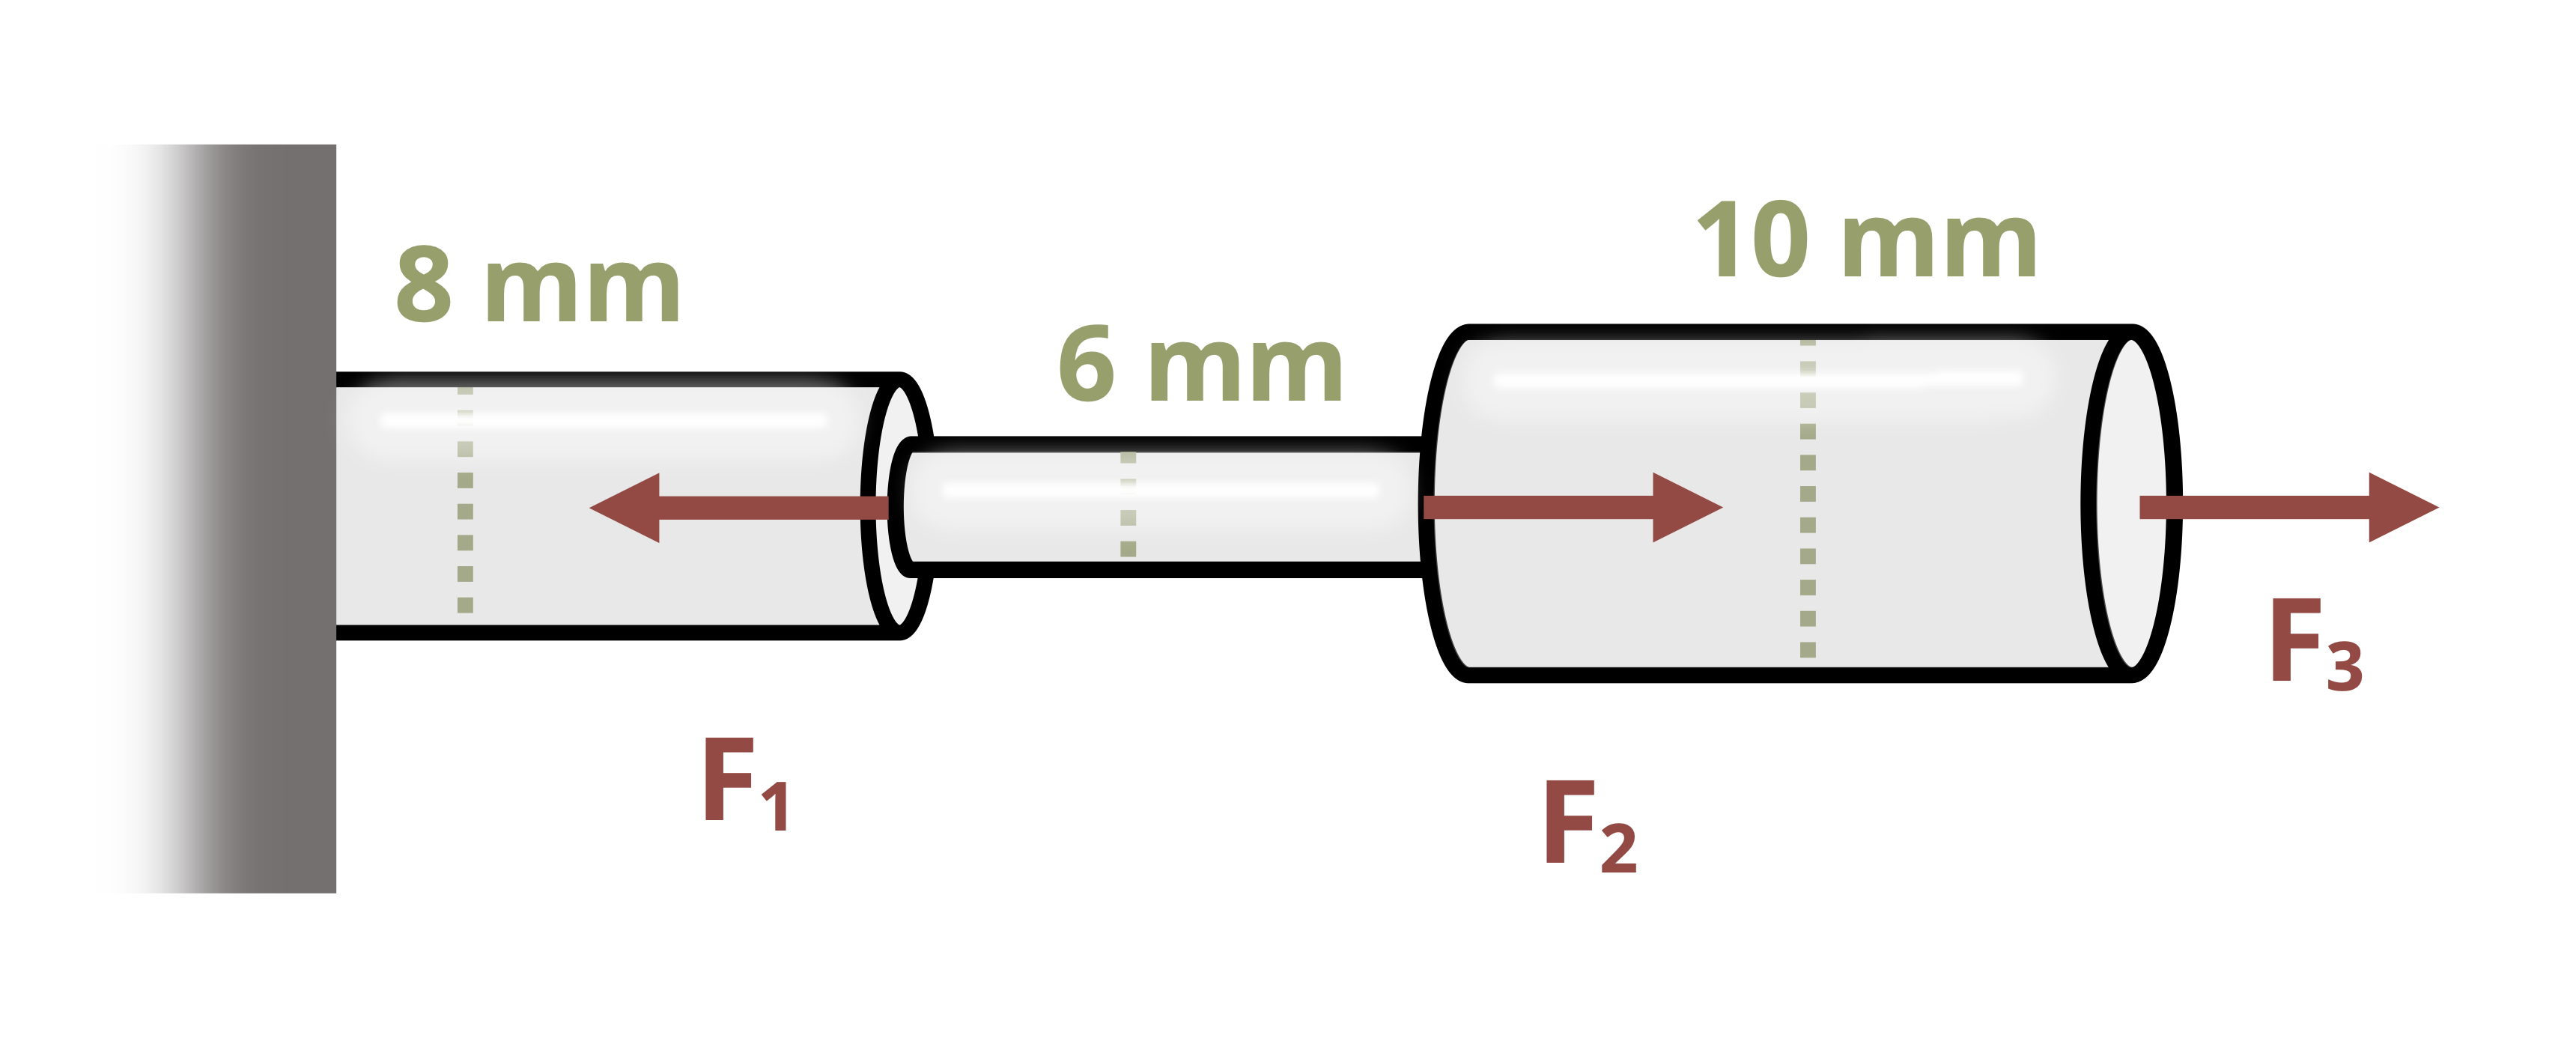
\includegraphics{images/138.png}

}

\caption{Figure 1: A series of solid circular bars are loaded with three
loads}

\end{figure}%

\begin{Shaded}
\begin{Highlighting}[]
\NormalTok{\#| standalone: true}
\NormalTok{\#| viewerHeight: 600}
\NormalTok{\#| components: [viewer]}

\NormalTok{from shiny import App, render, ui, reactive}
\NormalTok{import random}
\NormalTok{import asyncio}
\NormalTok{import io}
\NormalTok{import math}
\NormalTok{import string}
\NormalTok{from datetime import datetime}
\NormalTok{from pathlib import Path}


\NormalTok{def generate\_random\_letters(length):}
\NormalTok{    \# Generate a random string of letters of specified length}
\NormalTok{    return \textquotesingle{}\textquotesingle{}.join(random.choice(string.ascii\_lowercase) for \_ in range(length))  }

\NormalTok{problem\_ID="138"}
\NormalTok{F1=reactive.Value("\_\_")}
\NormalTok{F2=reactive.Value("\_\_")}
\NormalTok{F3=reactive.Value("\_\_")}
\NormalTok{d1=8}
\NormalTok{d2=6}
\NormalTok{d3=10}
\NormalTok{attempts=["Timestamp,Attempt,Answer,Feedback\textbackslash{}n"]}

\NormalTok{app\_ui = ui.page\_fluid(}
\NormalTok{    ui.markdown("**Please enter your ID number from your instructor and click to generate your problem**"),}
\NormalTok{    ui.input\_text("ID","", placeholder="Enter ID Number Here"),}
\NormalTok{    ui.input\_action\_button("generate\_problem", "Generate Problem", class\_="btn{-}primary"),}
\NormalTok{    ui.markdown("**Problem Statement**"),}
\NormalTok{    ui.output\_ui("ui\_problem\_statement"),}
\NormalTok{    ui.input\_text("answer","Your Answer in units of MPa", placeholder="Please enter your answer"),}
\NormalTok{    ui.input\_action\_button("submit", "Submit Answer", class\_="btn{-}primary"),}
\NormalTok{    ui.download\_button("download", "Download File to Submit", class\_="btn{-}success"),}
\NormalTok{)}


\NormalTok{def server(input, output, session):}
\NormalTok{    \# Initialize a counter for attempts}
\NormalTok{    attempt\_counter = reactive.Value(0)}
    
\NormalTok{    @output}
\NormalTok{    @render.ui}
\NormalTok{    def ui\_problem\_statement():}
\NormalTok{        return[ui.markdown(f"A series of solid circular bars are loaded with three loads as shown, F\textless{}sub\textgreater{}1\textless{}/sub\textgreater{} = \{F1()\} N, F\textless{}sub\textgreater{}2\textless{}/sub\textgreater{} = \{F2()\} N, and F\textless{}sub\textgreater{}3\textless{}/sub\textgreater{} = \{F3()\} N. What is the largest absolute normal stress in any bar?")]}
     
\NormalTok{    @reactive.Effect}
\NormalTok{    @reactive.event(input.generate\_problem)}
\NormalTok{    def randomize\_vars():}
\NormalTok{        random.seed(input.ID())}
\NormalTok{        F1.set(random.randrange(50, 70, 1))}
\NormalTok{        F2.set(random.randrange(10, 30, 1))}
\NormalTok{        F3.set(F1(){-}F2())}
        

\NormalTok{    @reactive.Effect}
\NormalTok{    @reactive.event(input.submit)}
\NormalTok{    def \_():}
\NormalTok{        attempt\_counter.set(attempt\_counter() + 1)  \# Increment the attempt counter on each submission.}
        
\NormalTok{        \# Calculate the instructor\textquotesingle{}s answer and determine if the user\textquotesingle{}s answer is correct.}
\NormalTok{        instr= (F1()/(math.pi*(d2/(1000*2))**2))/10**6}
        
\NormalTok{        if math.isclose(float(input.answer()), instr, rel\_tol=0.01):}
\NormalTok{            check = "*Correct*"}
\NormalTok{            correct\_indicator = "JL"}
\NormalTok{        else:}
\NormalTok{            check = "*Not Correct.*"}
\NormalTok{            correct\_indicator = "JG"}

\NormalTok{        \# Generate random parts for the encoded attempt.}
\NormalTok{        random\_start = generate\_random\_letters(4)}
\NormalTok{        random\_middle = generate\_random\_letters(4)}
\NormalTok{        random\_end = generate\_random\_letters(4)}
\NormalTok{        encoded\_attempt = f"\{random\_start\}\{problem\_ID\}{-}\{random\_middle\}\{attempt\_counter()\}\{correct\_indicator\}{-}\{random\_end\}\{input.ID()\}"}

\NormalTok{        \# Store the most recent encoded attempt in a reactive value so it persists across submissions}
\NormalTok{        session.encoded\_attempt = reactive.Value(encoded\_attempt)}

\NormalTok{        \# Append the attempt data to the attempts list without the encoded attempt}
\NormalTok{        attempts.append(f"\{datetime.now()\}, \{attempt\_counter()\}, \{input.answer()\}, \{check\}\textbackslash{}n")}

\NormalTok{        \# Show feedback to the user.}
\NormalTok{        feedback = ui.markdown(f"Your answer of \{input.answer()\} is \{check\}.")}
\NormalTok{        m = ui.modal(}
\NormalTok{            feedback,}
\NormalTok{            title="Feedback",}
\NormalTok{            easy\_close=True}
\NormalTok{        )}
\NormalTok{        ui.modal\_show(m)}

\NormalTok{    @session.download(filename=lambda: f"Problem\_Log{-}\{problem\_ID\}{-}\{input.ID()\}.csv")}
\NormalTok{    async def download():}
\NormalTok{        \# Start the CSV with the encoded attempt (without label)}
\NormalTok{        final\_encoded = session.encoded\_attempt() if session.encoded\_attempt is not None else "No attempts"}
\NormalTok{        yield f"\{final\_encoded\}\textbackslash{}n\textbackslash{}n"}
        
\NormalTok{        \# Write the header for the remaining CSV data once}
\NormalTok{        yield "Timestamp,Attempt,Answer,Feedback\textbackslash{}n"}
        
\NormalTok{        \# Write the attempts data, ensure that the header from the attempts list is not written again}
\NormalTok{        for attempt in attempts[1:]:  \# Skip the first element which is the header}
\NormalTok{            await asyncio.sleep(0.25)  \# This delay may not be necessary; adjust as needed}
\NormalTok{            yield attempt}


\NormalTok{\# App installation}
\NormalTok{app = App(app\_ui, server)}
\end{Highlighting}
\end{Shaded}

\chapter*{Problem 2.2}\label{problem-2.2}
\addcontentsline{toc}{chapter}{Problem 2.2}

\markboth{Problem 2.2}{Problem 2.2}

This is a dynamic rendering of the problem with dynamic variables based
on the username entered.

\section*{Problem Image}\label{problem-image-1}
\addcontentsline{toc}{section}{Problem Image}

\markright{Problem Image}

\begin{figure}[H]

{\centering 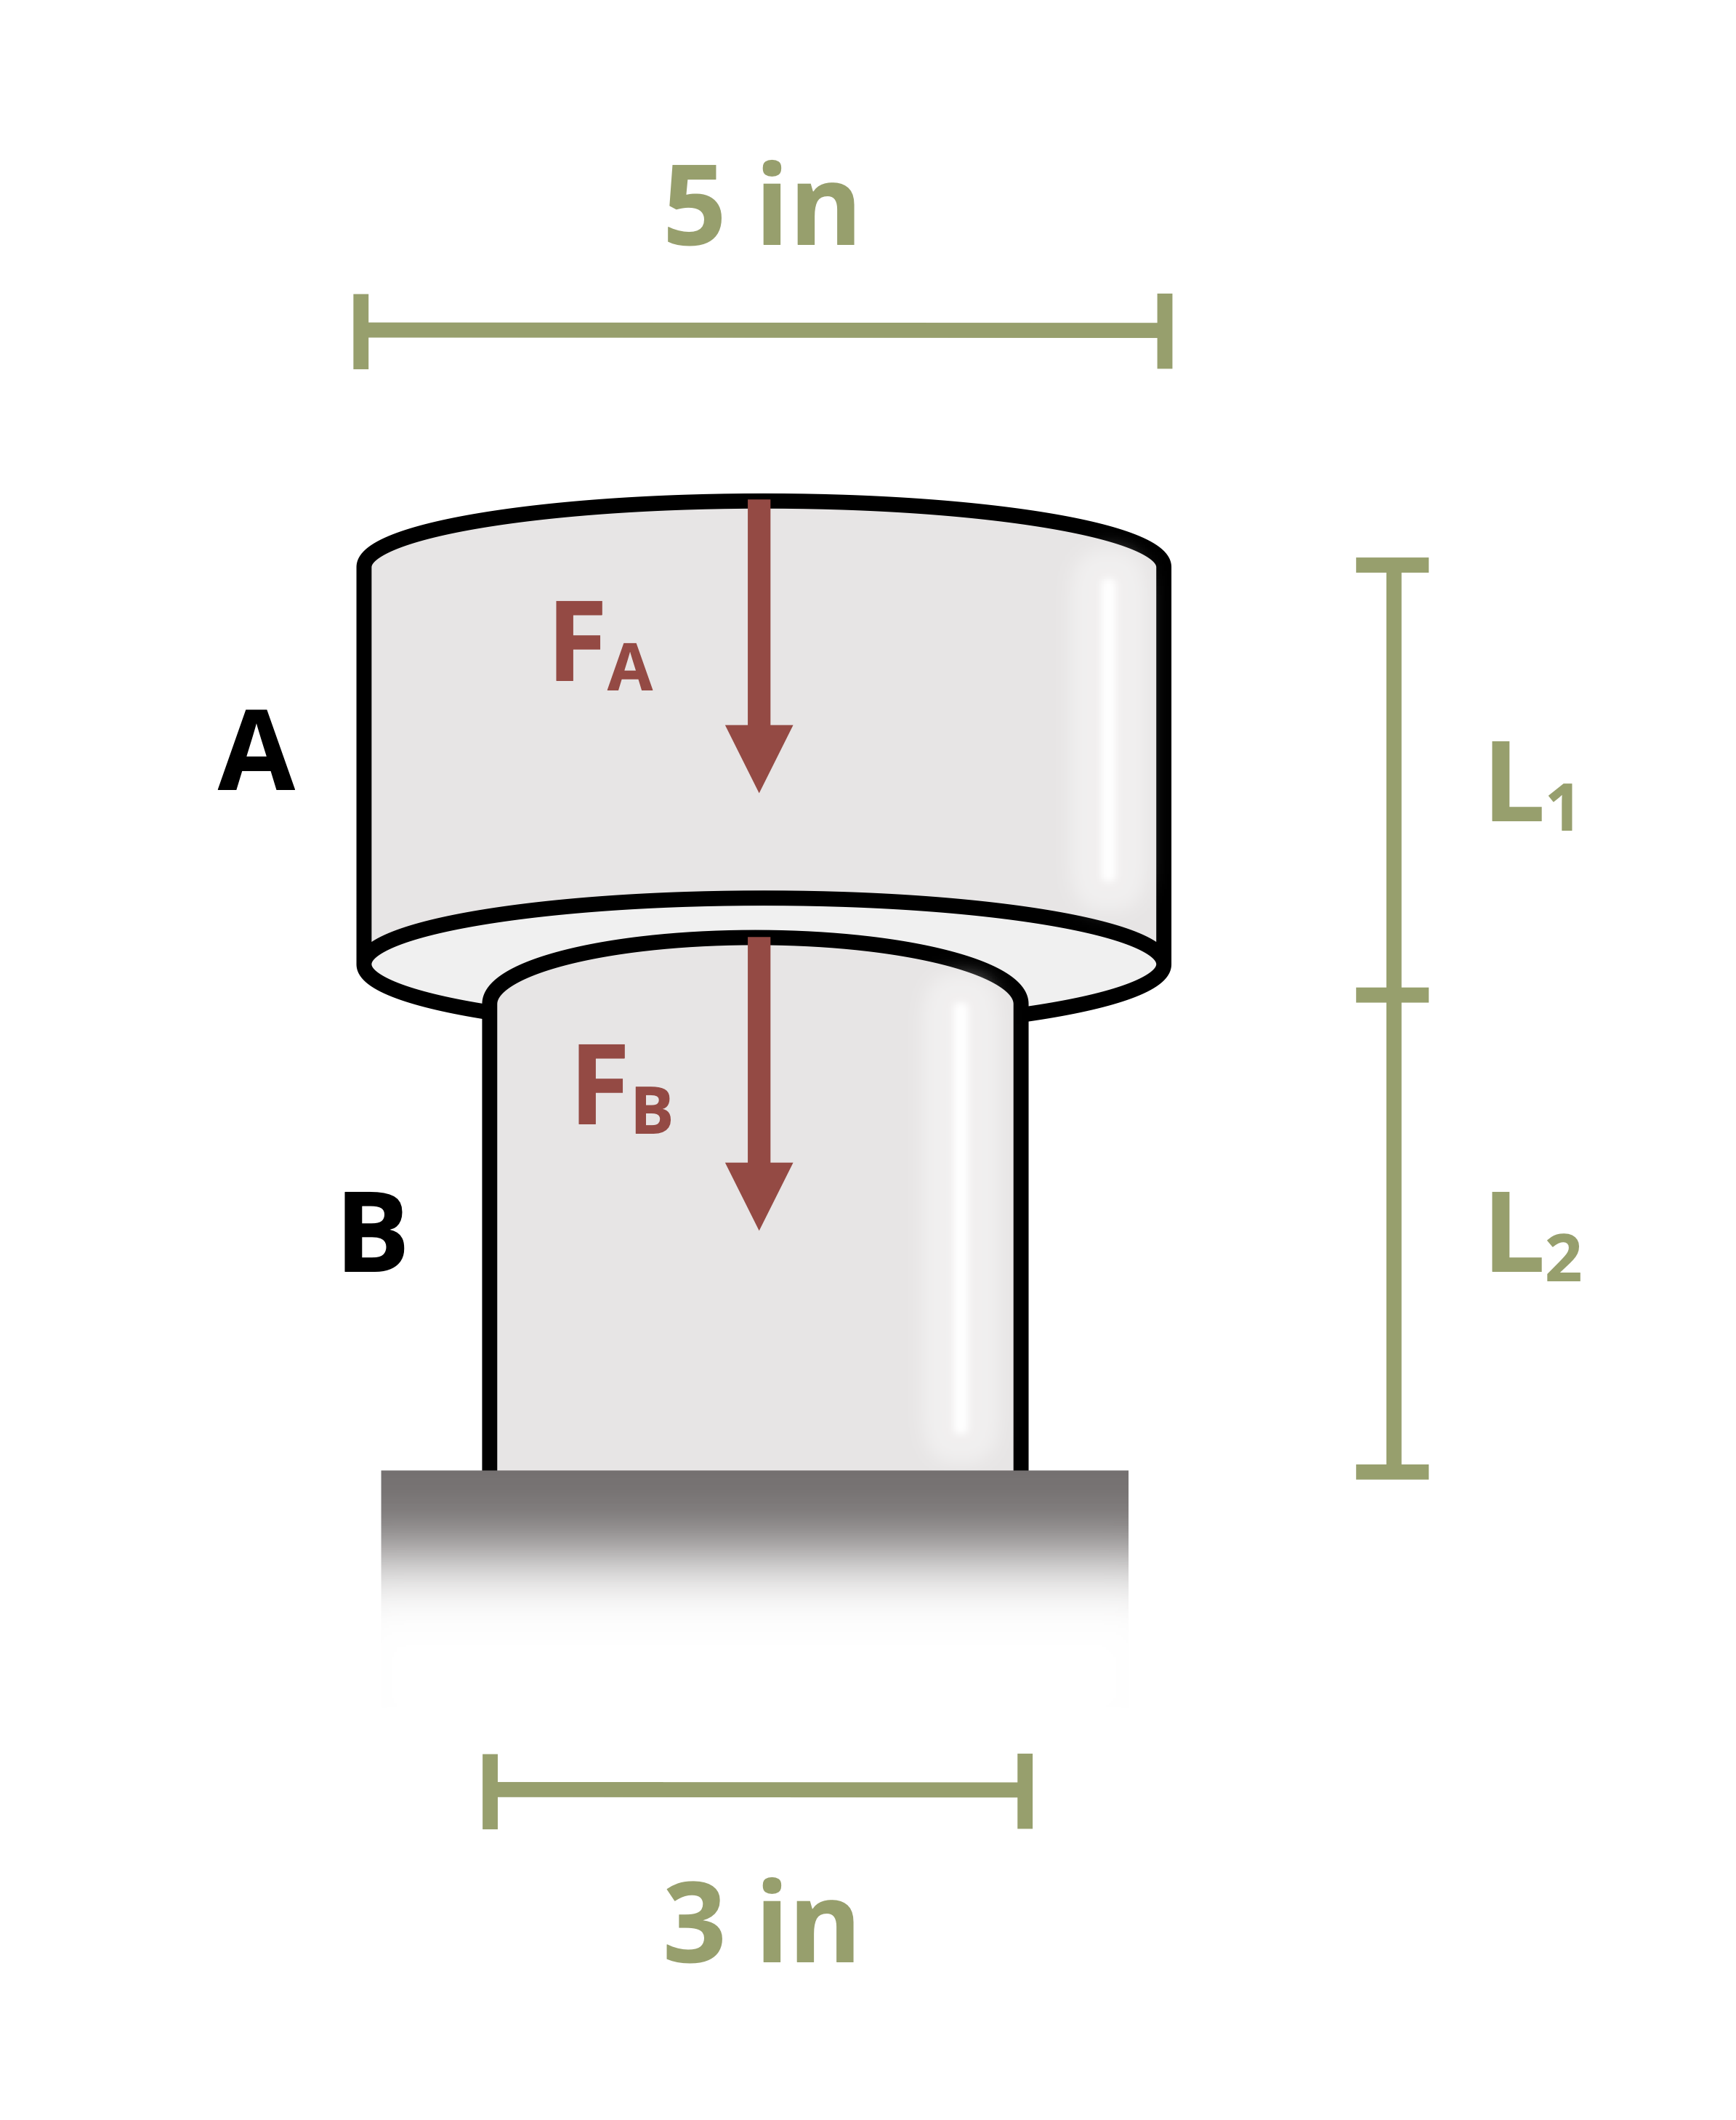
\includegraphics{images/139.png}

}

\caption{Figure 1: Two cylinders are stacked on top of each other.}

\end{figure}%

\begin{Shaded}
\begin{Highlighting}[]
\NormalTok{\#| standalone: true}
\NormalTok{\#| viewerHeight: 600}
\NormalTok{\#| components: [viewer]}

\NormalTok{from shiny import App, render, ui, reactive}
\NormalTok{import random}
\NormalTok{import asyncio}
\NormalTok{import io}
\NormalTok{import math}
\NormalTok{import string}
\NormalTok{from datetime import datetime}
\NormalTok{from pathlib import Path}

\NormalTok{def generate\_random\_letters(length):}
\NormalTok{    \# Generate a random string of letters of specified length}
\NormalTok{    return \textquotesingle{}\textquotesingle{}.join(random.choice(string.ascii\_lowercase) for \_ in range(length))  }

\NormalTok{problem\_ID="139"}
\NormalTok{L1=reactive.Value("\_\_")}
\NormalTok{L2=reactive.Value("\_\_")}
\NormalTok{FA=reactive.Value("\_\_")}
\NormalTok{FB=reactive.Value("\_\_")}
\NormalTok{E = 30*10**6}
  
\NormalTok{attempts=["Timestamp,Attempt,Answer,Feedback\textbackslash{}n"]}

\NormalTok{app\_ui = ui.page\_fluid(}
\NormalTok{    ui.markdown("**Please enter your ID number from your instructor and click to generate your problem**"),}
\NormalTok{    ui.input\_text("ID","", placeholder="Enter ID Number Here"),}
\NormalTok{    ui.input\_action\_button("generate\_problem", "Generate Problem", class\_="btn{-}primary"),}
\NormalTok{    ui.markdown("**Problem Statement**"),}
\NormalTok{    ui.output\_ui("ui\_problem\_statement"),}
\NormalTok{    ui.input\_text("answer","Your Answer in units of inches", placeholder="Please enter your answer"),}
\NormalTok{    ui.input\_action\_button("submit", "Submit Answer", class\_="btn{-}primary"),}
\NormalTok{    ui.download\_button("download", "Download File to Submit", class\_="btn{-}success"),}
\NormalTok{)}

\NormalTok{def server(input, output, session):}
\NormalTok{    \# Initialize a counter for attempts}
\NormalTok{    attempt\_counter = reactive.Value(0)}

\NormalTok{    @output}
\NormalTok{    @render.ui}
\NormalTok{    def ui\_problem\_statement():}
\NormalTok{        return[ui.markdown(f"Two cylinders are stacked on top of one another and two forces are applied at the top surface and at the joint between the cylinders as shown. If L\textless{}sub\textgreater{}1\textless{}/sub\textgreater{} = \{L1()\} in., L\textless{}sub\textgreater{}2\textless{}/sub\textgreater{} = \{L2()\} in., F\textless{}sub\textgreater{}A\textless{}/sub\textgreater{} = \{FA()\} lb, and F\textless{}sub\textgreater{}B\textless{}/sub\textgreater{} = \{FB()\} lb, find the total deflection in the stack of cylinders. Assume E = 30 x 10\textless{}sup\textgreater{}6\textless{}/sup\textgreater{} psi for both cylinders. ")]}
    
\NormalTok{    @reactive.Effect}
\NormalTok{    @reactive.event(input.generate\_problem)}
\NormalTok{    def randomize\_vars():}
\NormalTok{        random.seed(input.ID())}
\NormalTok{        FA.set(random.randrange(300, 700, 10))}
\NormalTok{        FB.set(random.randrange(100, 300, 10))}
\NormalTok{        L1.set(random.randrange(2, 7, 1))}
\NormalTok{        L2.set(L1() * 1.3)}
        
\NormalTok{    @reactive.Effect}
\NormalTok{    @reactive.event(input.submit)}
\NormalTok{    def \_():}
\NormalTok{        attempt\_counter.set(attempt\_counter() + 1)  \# Increment the attempt counter on each submission.}
    
\NormalTok{        instr= (FA()*L1())/((math.pi*(5/2)**2)*E) + ((FB()+FA())*L2())/((math.pi*(3/2)**2)*E)}
\NormalTok{        if math.isclose(float(input.answer()), instr, rel\_tol=0.01):}
\NormalTok{            check = "*Correct*"}
\NormalTok{            correct\_indicator = "JL"}
\NormalTok{        else:}
\NormalTok{            check = "*Not Correct.*"}
\NormalTok{            correct\_indicator = "JG"}

\NormalTok{        \# Generate random parts for the encoded attempt.}
\NormalTok{        random\_start = generate\_random\_letters(4)}
\NormalTok{        random\_middle = generate\_random\_letters(4)}
\NormalTok{        random\_end = generate\_random\_letters(4)}
\NormalTok{        encoded\_attempt = f"\{random\_start\}\{problem\_ID\}{-}\{random\_middle\}\{attempt\_counter()\}\{correct\_indicator\}{-}\{random\_end\}\{input.ID()\}"}

\NormalTok{        \# Store the most recent encoded attempt in a reactive value so it persists across submissions}
\NormalTok{        session.encoded\_attempt = reactive.Value(encoded\_attempt)}

\NormalTok{        \# Append the attempt data to the attempts list without the encoded attempt}
\NormalTok{        attempts.append(f"\{datetime.now()\}, \{attempt\_counter()\}, \{input.answer()\}, \{check\}\textbackslash{}n")}

\NormalTok{        \# Show feedback to the user.}
\NormalTok{        feedback = ui.markdown(f"Your answer of \{input.answer()\} is \{check\}.")}
\NormalTok{        m = ui.modal(}
\NormalTok{            feedback,}
\NormalTok{            title="Feedback",}
\NormalTok{            easy\_close=True}
\NormalTok{        )}
\NormalTok{        ui.modal\_show(m)}

\NormalTok{    @session.download(filename=lambda: f"Problem\_Log{-}\{problem\_ID\}{-}\{input.ID()\}.csv")}
\NormalTok{    async def download():}
\NormalTok{        \# Start the CSV with the encoded attempt (without label)}
\NormalTok{        final\_encoded = session.encoded\_attempt() if session.encoded\_attempt is not None else "No attempts"}
\NormalTok{        yield f"\{final\_encoded\}\textbackslash{}n\textbackslash{}n"}
        
\NormalTok{        \# Write the header for the remaining CSV data once}
\NormalTok{        yield "Timestamp,Attempt,Answer,Feedback\textbackslash{}n"}
        
\NormalTok{        \# Write the attempts data, ensure that the header from the attempts list is not written again}
\NormalTok{        for attempt in attempts[1:]:  \# Skip the first element which is the header}
\NormalTok{            await asyncio.sleep(0.25)  \# This delay may not be necessary; adjust as needed}
\NormalTok{            yield attempt}

\NormalTok{\# App installation}
\NormalTok{app = App(app\_ui, server)}
\end{Highlighting}
\end{Shaded}

\chapter*{Problem 2.3}\label{problem-2.3}
\addcontentsline{toc}{chapter}{Problem 2.3}

\markboth{Problem 2.3}{Problem 2.3}

This is a dynamic rendering of the problem with dynamic variables based
on the username entered.

\section*{Problem Image}\label{problem-image-2}
\addcontentsline{toc}{section}{Problem Image}

\markright{Problem Image}

\begin{figure}[H]

{\centering 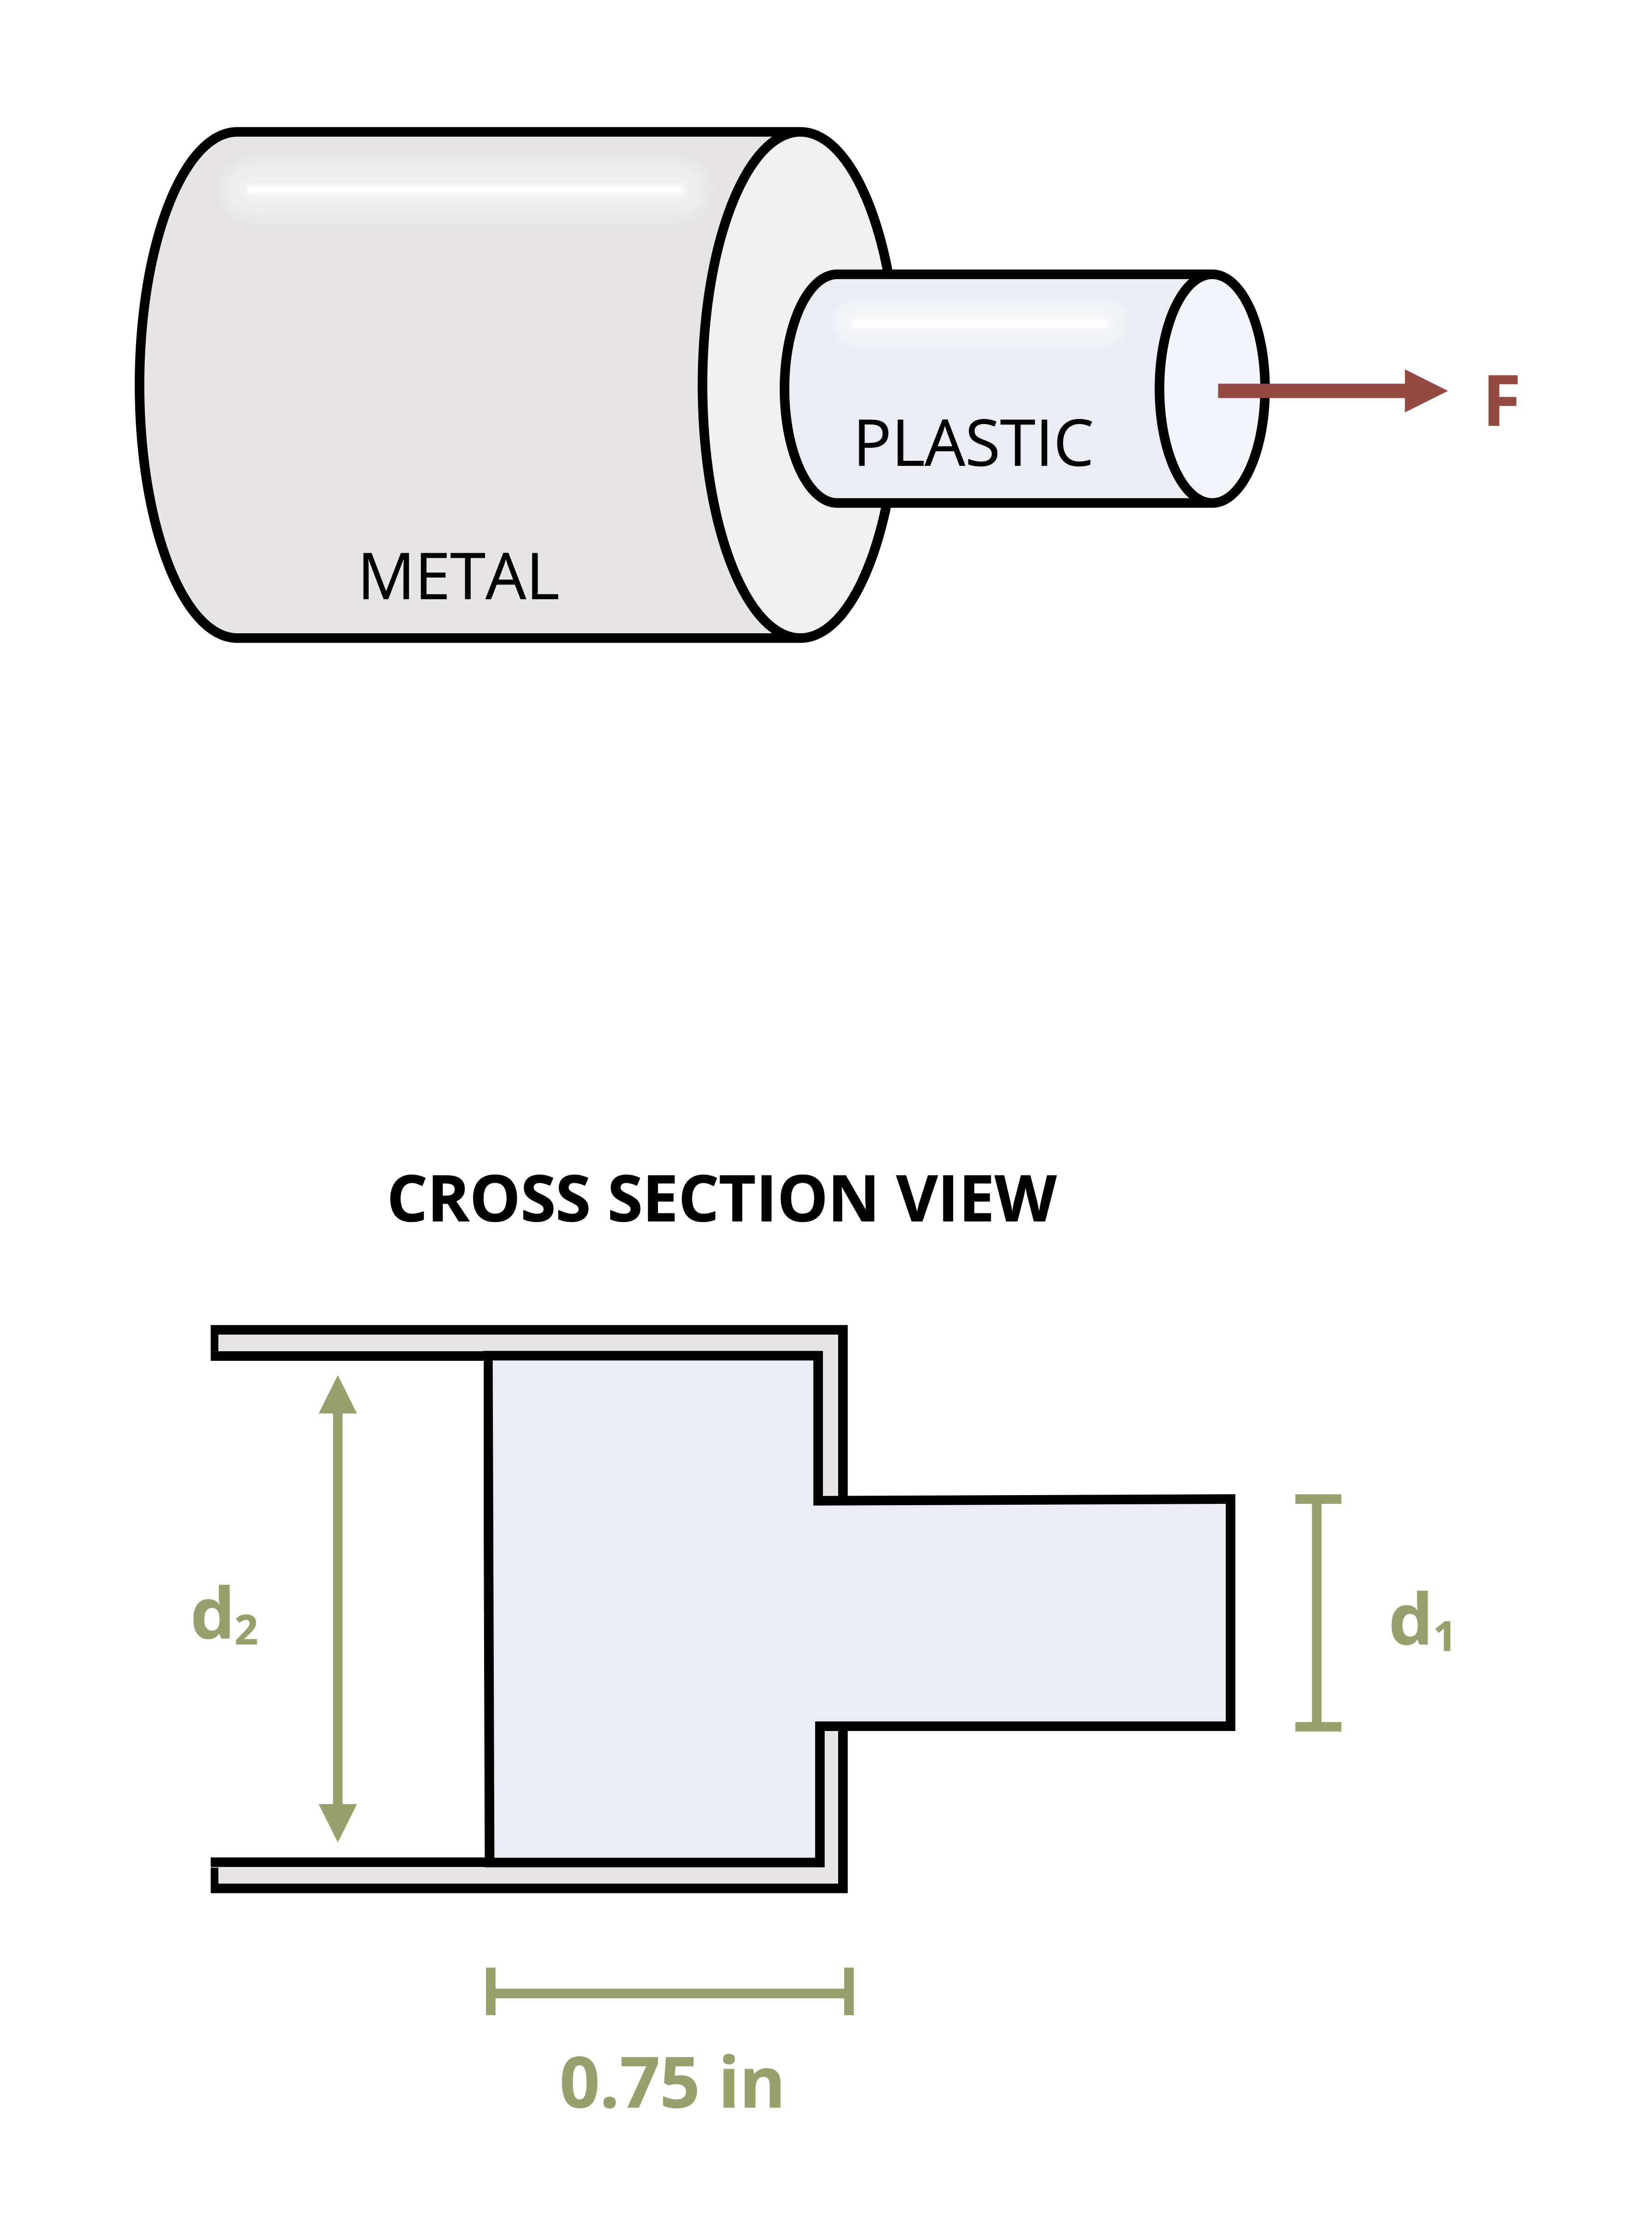
\includegraphics{images/144.png}

}

\caption{Figure 1: A plastic cylindrical peg is constrained by a metal
cap}

\end{figure}%

\begin{Shaded}
\begin{Highlighting}[]
\NormalTok{\#| standalone: true}
\NormalTok{\#| viewerHeight: 600}
\NormalTok{\#| components: [viewer]}

\NormalTok{from shiny import App, render, ui, reactive}
\NormalTok{import random}
\NormalTok{import asyncio}
\NormalTok{import io}
\NormalTok{import math}
\NormalTok{import string}
\NormalTok{from datetime import datetime}
\NormalTok{from pathlib import Path}

\NormalTok{def generate\_random\_letters(length):}
\NormalTok{    \# Generate a random string of letters of specified length}
\NormalTok{    return \textquotesingle{}\textquotesingle{}.join(random.choice(string.ascii\_lowercase) for \_ in range(length))}

\NormalTok{problem\_ID="144"}
\NormalTok{F=reactive.Value("\_\_")}
\NormalTok{d1=reactive.Value("\_\_")}
\NormalTok{d2=reactive.Value("\_\_")}

\NormalTok{attempts=["Timestamp,Attempt,Answer,Feedback\textbackslash{}n"]}

\NormalTok{app\_ui = ui.page\_fluid(}
\NormalTok{    ui.markdown("**Please enter your ID number from your instructor and click to generate your problem**"),}
\NormalTok{    ui.input\_text("ID","", placeholder="Enter ID Number Here"),}
\NormalTok{    ui.input\_action\_button("generate\_problem", "Generate Problem", class\_="btn{-}primary"),}
\NormalTok{    ui.markdown("**Problem Statement**"),}
\NormalTok{    ui.output\_ui("ui\_problem\_statement"),}
\NormalTok{    ui.input\_text("answer","Your Answer in units of psi", placeholder="Please enter your answer"),}
\NormalTok{    ui.input\_action\_button("submit", "Submit Answer", class\_="btn{-}primary"),}
\NormalTok{    ui.download\_button("download", "Download File to Submit", class\_="btn{-}success"),}
\NormalTok{)}


\NormalTok{def server(input, output, session):}
\NormalTok{    \# Initialize a counter for attempts}
\NormalTok{    attempt\_counter = reactive.Value(0)}

\NormalTok{    @output}
\NormalTok{    @render.ui}
\NormalTok{    def ui\_problem\_statement():}
\NormalTok{        return[ui.markdown(f"A plastic cylindrical peg is constrained by a metal cap as shown. An axial load of F = \{F()\} lb is applied to the peg. If d\textless{}sub\textgreater{}1\textless{}/sub\textgreater{} = \{d1()\} in and d\textless{}sub\textgreater{}2\textless{}/sub\textgreater{} = \{d2()\} in, determine the largest normal stress in the peg. Assume the axial load is evenly distributed across the peg and that the metal cap is fixed and does not move.")]}
    
\NormalTok{    @reactive.Effect}
\NormalTok{    @reactive.event(input.generate\_problem)}
\NormalTok{    def randomize\_vars():}
\NormalTok{        random.seed(input.ID())}
\NormalTok{        F.set(random.randrange(20, 80, 5))}
\NormalTok{        d1.set(random.randrange(3, 8, 1)/10)}
\NormalTok{        d2.set(round(d1() * 1.6, 2))}
        
 
\NormalTok{    @reactive.Effect}
\NormalTok{    @reactive.event(input.submit)}
\NormalTok{    def \_():}
\NormalTok{        attempt\_counter.set(attempt\_counter() + 1)  \# Increment the attempt counter on each submission.}
\NormalTok{        instr= F()/(math.pi*((d1()/2)**2))}
\NormalTok{        \#check=math.isclose(float(input.answer()),instr,rel\_tol=0.001)}
        
\NormalTok{        if math.isclose(float(input.answer()), instr, rel\_tol=0.01):}
\NormalTok{            check = "*Correct*"}
\NormalTok{            correct\_indicator = "JL"}
\NormalTok{        else:}
\NormalTok{            check = "*Not Correct.*"}
\NormalTok{            correct\_indicator = "JG"}

\NormalTok{        \# Generate random parts for the encoded attempt.}
\NormalTok{        random\_start = generate\_random\_letters(4)}
\NormalTok{        random\_middle = generate\_random\_letters(4)}
\NormalTok{        random\_end = generate\_random\_letters(4)}
\NormalTok{        encoded\_attempt = f"\{random\_start\}\{problem\_ID\}{-}\{random\_middle\}\{attempt\_counter()\}\{correct\_indicator\}{-}\{random\_end\}\{input.ID()\}"}

\NormalTok{        \# Store the most recent encoded attempt in a reactive value so it persists across submissions}
\NormalTok{        session.encoded\_attempt = reactive.Value(encoded\_attempt)}

\NormalTok{        \# Append the attempt data to the attempts list without the encoded attempt}
\NormalTok{        attempts.append(f"\{datetime.now()\}, \{attempt\_counter()\}, \{input.answer()\}, \{check\}\textbackslash{}n")}

\NormalTok{        \# Show feedback to the user.}
\NormalTok{        feedback = ui.markdown(f"Your answer of \{input.answer()\} is \{check\}.")}
\NormalTok{        m = ui.modal(}
\NormalTok{            feedback,}
\NormalTok{            title="Feedback",}
\NormalTok{            easy\_close=True}
\NormalTok{        )}
\NormalTok{        ui.modal\_show(m)}

\NormalTok{    @session.download(filename=lambda: f"Problem\_Log{-}\{problem\_ID\}{-}\{input.ID()\}.csv")}
\NormalTok{    async def download():}
\NormalTok{        \# Start the CSV with the encoded attempt (without label)}
\NormalTok{        final\_encoded = session.encoded\_attempt() if session.encoded\_attempt is not None else "No attempts"}
\NormalTok{        yield f"\{final\_encoded\}\textbackslash{}n\textbackslash{}n"}
        
\NormalTok{        \# Write the header for the remaining CSV data once}
\NormalTok{        yield "Timestamp,Attempt,Answer,Feedback\textbackslash{}n"}
        
\NormalTok{        \# Write the attempts data, ensure that the header from the attempts list is not written again}
\NormalTok{        for attempt in attempts[1:]:  \# Skip the first element which is the header}
\NormalTok{            await asyncio.sleep(0.25)  \# This delay may not be necessary; adjust as needed}
\NormalTok{            yield attempt}


\NormalTok{\# App installation}
\NormalTok{app = App(app\_ui, server)}
\end{Highlighting}
\end{Shaded}

\chapter*{Problem 2.4}\label{problem-2.4}
\addcontentsline{toc}{chapter}{Problem 2.4}

\markboth{Problem 2.4}{Problem 2.4}

This is a dynamic rendering of the problem with dynamic variables based
on the username entered.

\section*{Problem Image}\label{problem-image-3}
\addcontentsline{toc}{section}{Problem Image}

\markright{Problem Image}

\begin{figure}[H]

{\centering 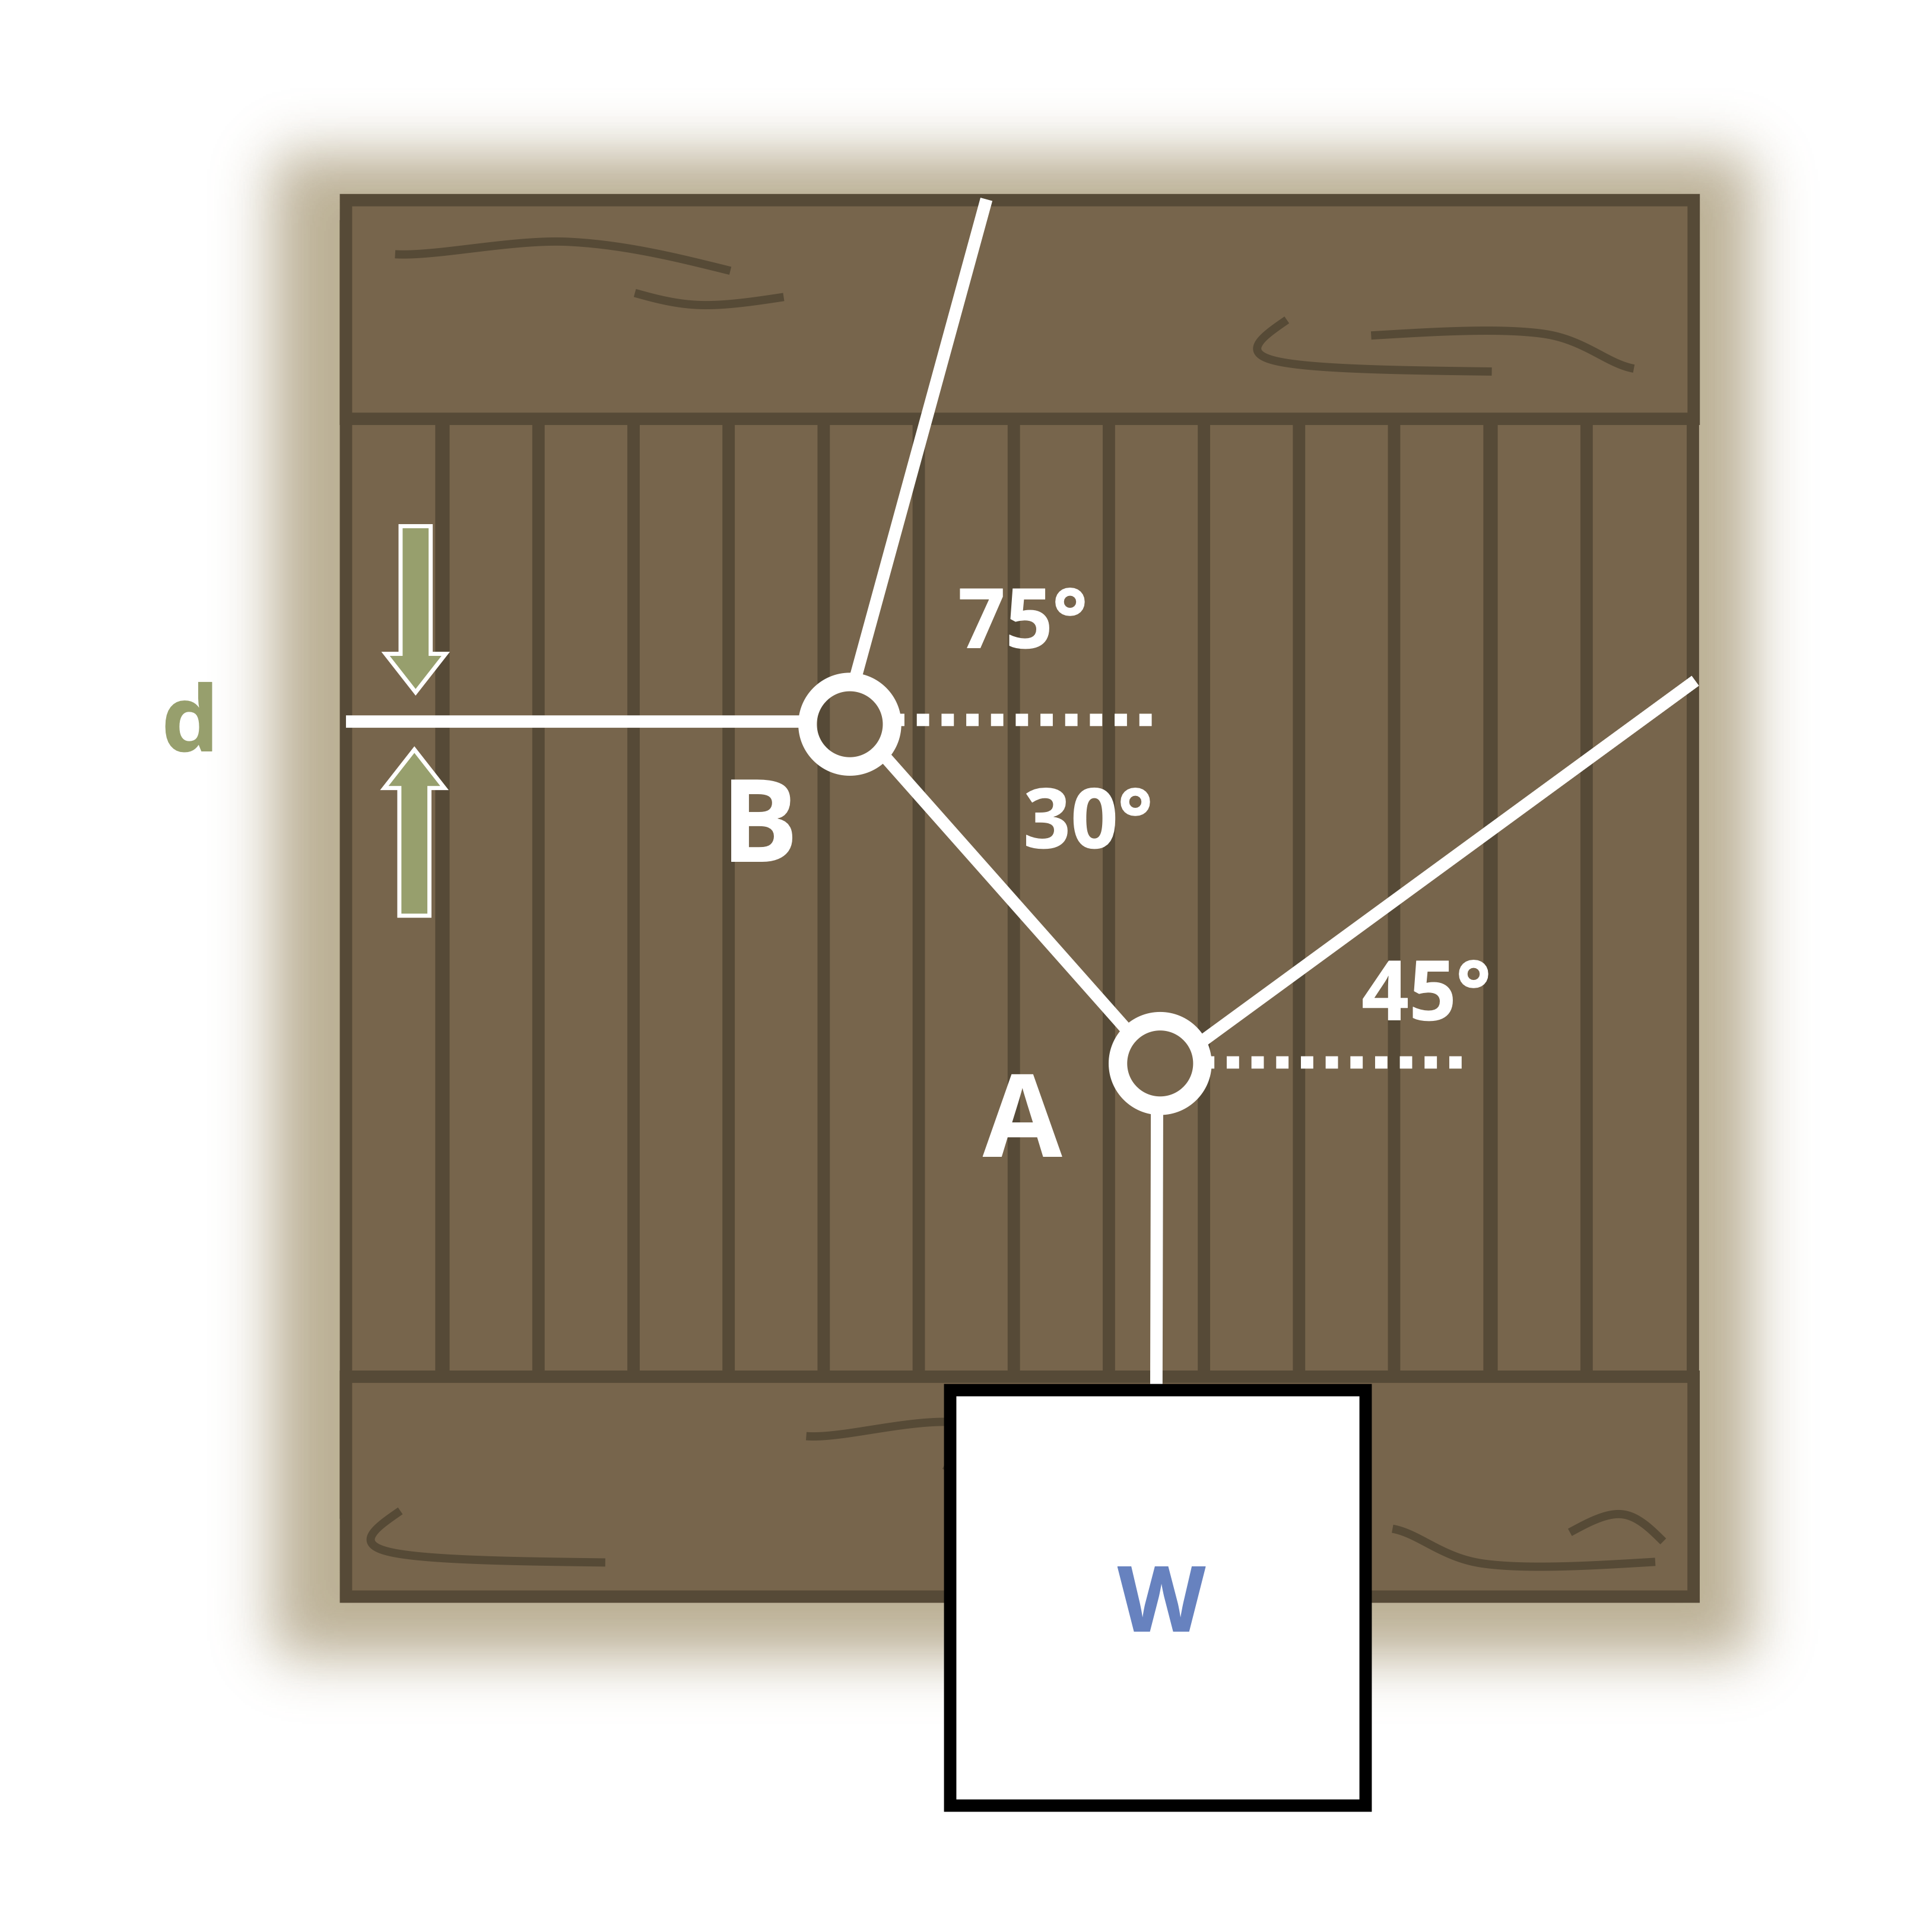
\includegraphics{images/146.png}

}

\caption{Figure 1: A crate is suspended by a set of cables.}

\end{figure}%

\begin{Shaded}
\begin{Highlighting}[]
\NormalTok{\#| standalone: true}
\NormalTok{\#| viewerHeight: 600}
\NormalTok{\#| components: [viewer]}

\NormalTok{from shiny import App, render, ui, reactive}
\NormalTok{import random}
\NormalTok{import asyncio}
\NormalTok{import io}
\NormalTok{import math}
\NormalTok{import string}
\NormalTok{from datetime import datetime}
\NormalTok{from pathlib import Path}


\NormalTok{def generate\_random\_letters(length):}
\NormalTok{    \# Generate a random string of letters of specified length}
\NormalTok{    return \textquotesingle{}\textquotesingle{}.join(random.choice(string.ascii\_lowercase) for \_ in range(length)) }

\NormalTok{problem\_ID="146"}
\NormalTok{W=reactive.Value("\_\_")}
\NormalTok{d=reactive.Value("\_\_")}
\NormalTok{angle1=math.radians(45)}
\NormalTok{angle2=math.radians(30)}
\NormalTok{angle3=math.radians(75)}

\NormalTok{attempts=["Timestamp,Attempt,Answer,Feedback\textbackslash{}n"]}

\NormalTok{app\_ui = ui.page\_fluid(}
\NormalTok{    ui.markdown("**Please enter your ID number from your instructor and click to generate your problem**"),}
\NormalTok{    ui.input\_text("ID","", placeholder="Enter ID Number Here"),}
\NormalTok{    ui.input\_action\_button("generate\_problem", "Generate Problem", class\_="btn{-}primary"),}
\NormalTok{    ui.markdown("**Problem Statement**"),}
\NormalTok{    ui.output\_ui("ui\_problem\_statement"),}
\NormalTok{    ui.input\_text("answer","Your Answer in units of GPa", placeholder="Please enter your answer"),}
\NormalTok{    ui.input\_action\_button("submit", "Submit Answer", class\_="btn{-}primary"),}
\NormalTok{    ui.download\_button("download", "Download File to Submit", class\_="btn{-}success"),}
\NormalTok{)}


\NormalTok{def server(input, output, session):}
\NormalTok{    \# Initialize a counter for attempts}
\NormalTok{    attempt\_counter = reactive.Value(0)}

\NormalTok{    @output}
\NormalTok{    @render.ui}
\NormalTok{    def ui\_problem\_statement():}
\NormalTok{        return[ui.markdown(f"A crate weighing \{W()\} kN is suspended by a set of cables. The diameter of each cable is \{d()\}  mm. What is the maximum stress in any cable, exluding the cable attached to the crate.")]}
    
\NormalTok{    @reactive.Effect}
\NormalTok{    @reactive.event(input.generate\_problem)}
\NormalTok{    def randomize\_vars():}
\NormalTok{        random.seed(input.ID())}
\NormalTok{        W.set(random.randrange(30, 90, 1))}
\NormalTok{        d.set(random.randrange(20, 90, 1)/10)}
        

\NormalTok{    @reactive.Effect}
\NormalTok{    @reactive.event(input.submit)}
\NormalTok{    def \_():}
\NormalTok{        attempt\_counter.set(attempt\_counter() + 1)  \# Increment the attempt counter on each submission.}
    
\NormalTok{        R1 = W()/(((math.cos(angle1)/math.cos(angle2))*math.sin(angle2))+math.sin(angle1))}
\NormalTok{        instr= (R1*10**3/(math.pi*((d()/(1000*2))**2)))/10**9}
\NormalTok{        if math.isclose(float(input.answer()), instr, rel\_tol=0.01):}
\NormalTok{            check = "*Correct*"}
\NormalTok{            correct\_indicator = "JL"}
\NormalTok{        else:}
\NormalTok{            check = "*Not Correct.*"}
\NormalTok{            correct\_indicator = "JG"}

\NormalTok{        \# Generate random parts for the encoded attempt.}
\NormalTok{        random\_start = generate\_random\_letters(4)}
\NormalTok{        random\_middle = generate\_random\_letters(4)}
\NormalTok{        random\_end = generate\_random\_letters(4)}
\NormalTok{        encoded\_attempt = f"\{random\_start\}\{problem\_ID\}{-}\{random\_middle\}\{attempt\_counter()\}\{correct\_indicator\}{-}\{random\_end\}\{input.ID()\}"}

\NormalTok{        \# Store the most recent encoded attempt in a reactive value so it persists across submissions}
\NormalTok{        session.encoded\_attempt = reactive.Value(encoded\_attempt)}

\NormalTok{        \# Append the attempt data to the attempts list without the encoded attempt}
\NormalTok{        attempts.append(f"\{datetime.now()\}, \{attempt\_counter()\}, \{input.answer()\}, \{check\}\textbackslash{}n")}

\NormalTok{        \# Show feedback to the user.}
\NormalTok{        feedback = ui.markdown(f"Your answer of \{input.answer()\} is \{check\}.")}
\NormalTok{        m = ui.modal(}
\NormalTok{            feedback,}
\NormalTok{            title="Feedback",}
\NormalTok{            easy\_close=True}
\NormalTok{        )}
\NormalTok{        ui.modal\_show(m)}

\NormalTok{    @session.download(filename=lambda: f"Problem\_Log{-}\{problem\_ID\}{-}\{input.ID()\}.csv")}
\NormalTok{    async def download():}
\NormalTok{        \# Start the CSV with the encoded attempt (without label)}
\NormalTok{        final\_encoded = session.encoded\_attempt() if session.encoded\_attempt is not None else "No attempts"}
\NormalTok{        yield f"\{final\_encoded\}\textbackslash{}n\textbackslash{}n"}
        
\NormalTok{        \# Write the header for the remaining CSV data once}
\NormalTok{        yield "Timestamp,Attempt,Answer,Feedback\textbackslash{}n"}
        
\NormalTok{        \# Write the attempts data, ensure that the header from the attempts list is not written again}
\NormalTok{        for attempt in attempts[1:]:  \# Skip the first element which is the header}
\NormalTok{            await asyncio.sleep(0.25)  \# This delay may not be necessary; adjust as needed}
\NormalTok{            yield attempt}


\NormalTok{\# App installation}
\NormalTok{app = App(app\_ui, server)}
\end{Highlighting}
\end{Shaded}

\chapter*{Problem 2.47}\label{problem-2.47}
\addcontentsline{toc}{chapter}{Problem 2.47}

\markboth{Problem 2.47}{Problem 2.47}

This is a dynamic rendering of the problem with dynamic variables based
on the username entered.

\section*{Problem Image}\label{problem-image-4}
\addcontentsline{toc}{section}{Problem Image}

\markright{Problem Image}

\begin{figure}[H]

{\centering 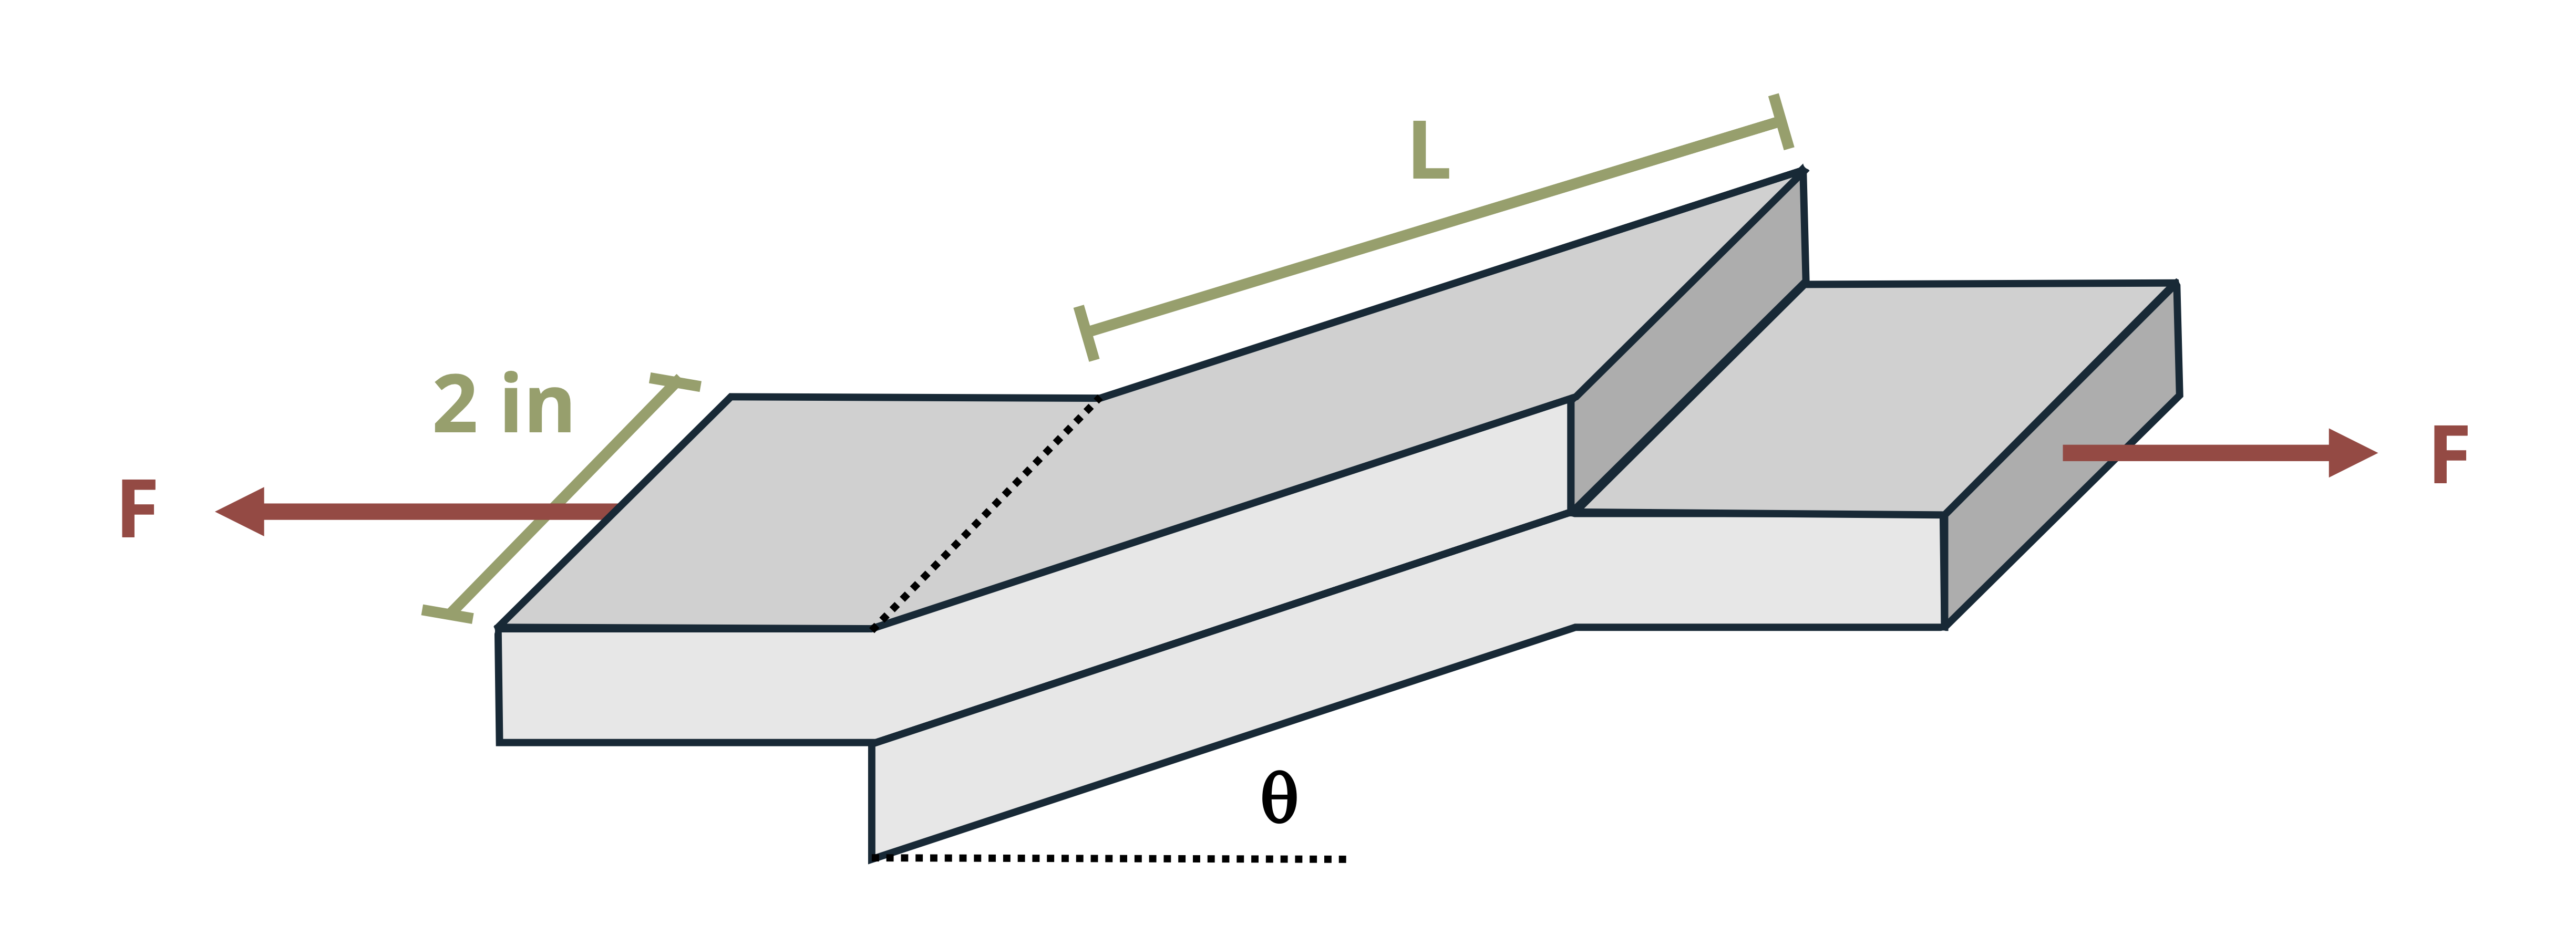
\includegraphics{images/153.png}

}

\caption{Figure 1: Two slanted brackets are glued together.}

\end{figure}%

\begin{Shaded}
\begin{Highlighting}[]
\NormalTok{\#| standalone: true}
\NormalTok{\#| viewerHeight: 600}
\NormalTok{\#| components: [viewer]}

\NormalTok{from shiny import App, render, ui, reactive}
\NormalTok{import random}
\NormalTok{import asyncio}
\NormalTok{import io}
\NormalTok{import math}
\NormalTok{import string}
\NormalTok{from datetime import datetime}
\NormalTok{from pathlib import Path}

\NormalTok{def generate\_random\_letters(length):}
\NormalTok{    \# Generate a random string of letters of specified length}
\NormalTok{    return \textquotesingle{}\textquotesingle{}.join(random.choice(string.ascii\_lowercase) for \_ in range(length))  }

\NormalTok{problem\_ID="153"}
\NormalTok{F=reactive.Value("\_\_")}
\NormalTok{L=reactive.Value("\_\_")}
\NormalTok{Θ=reactive.Value("\_\_")}

\NormalTok{attempts=["Timestamp,Attempt,Answer,Feedback\textbackslash{}n"]}

\NormalTok{app\_ui = ui.page\_fluid(}
\NormalTok{    ui.markdown("**Please enter your ID number from your instructor and click to generate your problem**"),}
\NormalTok{    ui.input\_text("ID","", placeholder="Enter ID Number Here"),}
\NormalTok{    ui.input\_action\_button("generate\_problem", "Generate Problem", class\_="btn{-}primary"),}
\NormalTok{    ui.markdown("**Problem Statement**"),}
\NormalTok{    ui.output\_ui("ui\_problem\_statement"),}
\NormalTok{    ui.input\_text("answer","Your Answer in units of psi", placeholder="Please enter your answer"),}
\NormalTok{    ui.input\_action\_button("submit", "Submit Answer", class\_="btn{-}primary"),}
\NormalTok{    ui.download\_button("download", "Download File to Submit", class\_="btn{-}success"),}
\NormalTok{)}

\NormalTok{def server(input, output, session):}
\NormalTok{    \# Initialize a counter for attempts}
\NormalTok{    attempt\_counter = reactive.Value(0)}

\NormalTok{    @output}
\NormalTok{    @render.ui}
\NormalTok{    def ui\_problem\_statement():}
\NormalTok{        return[ui.markdown(f"Two slanted brackets are glued together as shown. If F = \{F()\} lb, L = \{L()\} in., and Θ = \{Θ()\} °, determine the shear stress parallel to the inclined plane. Assume loads are inline and there is no rotation.")]}
    
\NormalTok{    @reactive.Effect}
\NormalTok{    @reactive.event(input.generate\_problem)}
\NormalTok{    def randomize\_vars():}
\NormalTok{        random.seed(input.ID())}
\NormalTok{        F.set(random.randrange(200, 800, 10))}
\NormalTok{        L.set(random.randrange(20, 80, 1)/10)}
\NormalTok{        Θ.set(random.randrange(15, 30, 1))}
        
\NormalTok{    @reactive.Effect}
\NormalTok{    @reactive.event(input.submit)}
\NormalTok{    def \_():}
\NormalTok{        attempt\_counter.set(attempt\_counter() + 1)  \# Increment the attempt counter on each submission.}
    
\NormalTok{        instr= (F()*math.cos(math.radians(Θ()))/(L()*2))}
\NormalTok{        if math.isclose(float(input.answer()), instr, rel\_tol=0.01):}
\NormalTok{            check = "*Correct*"}
\NormalTok{            correct\_indicator = "JL"}
\NormalTok{        else:}
\NormalTok{            check = "*Not Correct.*"}
\NormalTok{            correct\_indicator = "JG"}

\NormalTok{        \# Generate random parts for the encoded attempt.}
\NormalTok{        random\_start = generate\_random\_letters(4)}
\NormalTok{        random\_middle = generate\_random\_letters(4)}
\NormalTok{        random\_end = generate\_random\_letters(4)}
\NormalTok{        encoded\_attempt = f"\{random\_start\}\{problem\_ID\}{-}\{random\_middle\}\{attempt\_counter()\}\{correct\_indicator\}{-}\{random\_end\}\{input.ID()\}"}

\NormalTok{        \# Store the most recent encoded attempt in a reactive value so it persists across submissions}
\NormalTok{        session.encoded\_attempt = reactive.Value(encoded\_attempt)}

\NormalTok{        \# Append the attempt data to the attempts list without the encoded attempt}
\NormalTok{        attempts.append(f"\{datetime.now()\}, \{attempt\_counter()\}, \{input.answer()\}, \{check\}\textbackslash{}n")}

\NormalTok{        \# Show feedback to the user.}
\NormalTok{        feedback = ui.markdown(f"Your answer of \{input.answer()\} is \{check\}.")}
\NormalTok{        m = ui.modal(}
\NormalTok{            feedback,}
\NormalTok{            title="Feedback",}
\NormalTok{            easy\_close=True}
\NormalTok{        )}
\NormalTok{        ui.modal\_show(m)}

\NormalTok{    @session.download(filename=lambda: f"Problem\_Log{-}\{problem\_ID\}{-}\{input.ID()\}.csv")}
\NormalTok{    async def download():}
\NormalTok{        \# Start the CSV with the encoded attempt (without label)}
\NormalTok{        final\_encoded = session.encoded\_attempt() if session.encoded\_attempt is not None else "No attempts"}
\NormalTok{        yield f"\{final\_encoded\}\textbackslash{}n\textbackslash{}n"}
        
\NormalTok{        \# Write the header for the remaining CSV data once}
\NormalTok{        yield "Timestamp,Attempt,Answer,Feedback\textbackslash{}n"}
        
\NormalTok{        \# Write the attempts data, ensure that the header from the attempts list is not written again}
\NormalTok{        for attempt in attempts[1:]:  \# Skip the first element which is the header}
\NormalTok{            await asyncio.sleep(0.25)  \# This delay may not be necessary; adjust as needed}
\NormalTok{            yield attempt}

\NormalTok{\# App installation}
\NormalTok{app = App(app\_ui, server)}
\end{Highlighting}
\end{Shaded}

\chapter*{Problem 2.48}\label{problem-2.48}
\addcontentsline{toc}{chapter}{Problem 2.48}

\markboth{Problem 2.48}{Problem 2.48}

This is a dynamic rendering of the problem with dynamic variables based
on the username entered.

\section*{Problem Image}\label{problem-image-5}
\addcontentsline{toc}{section}{Problem Image}

\markright{Problem Image}

\begin{figure}[H]

{\centering 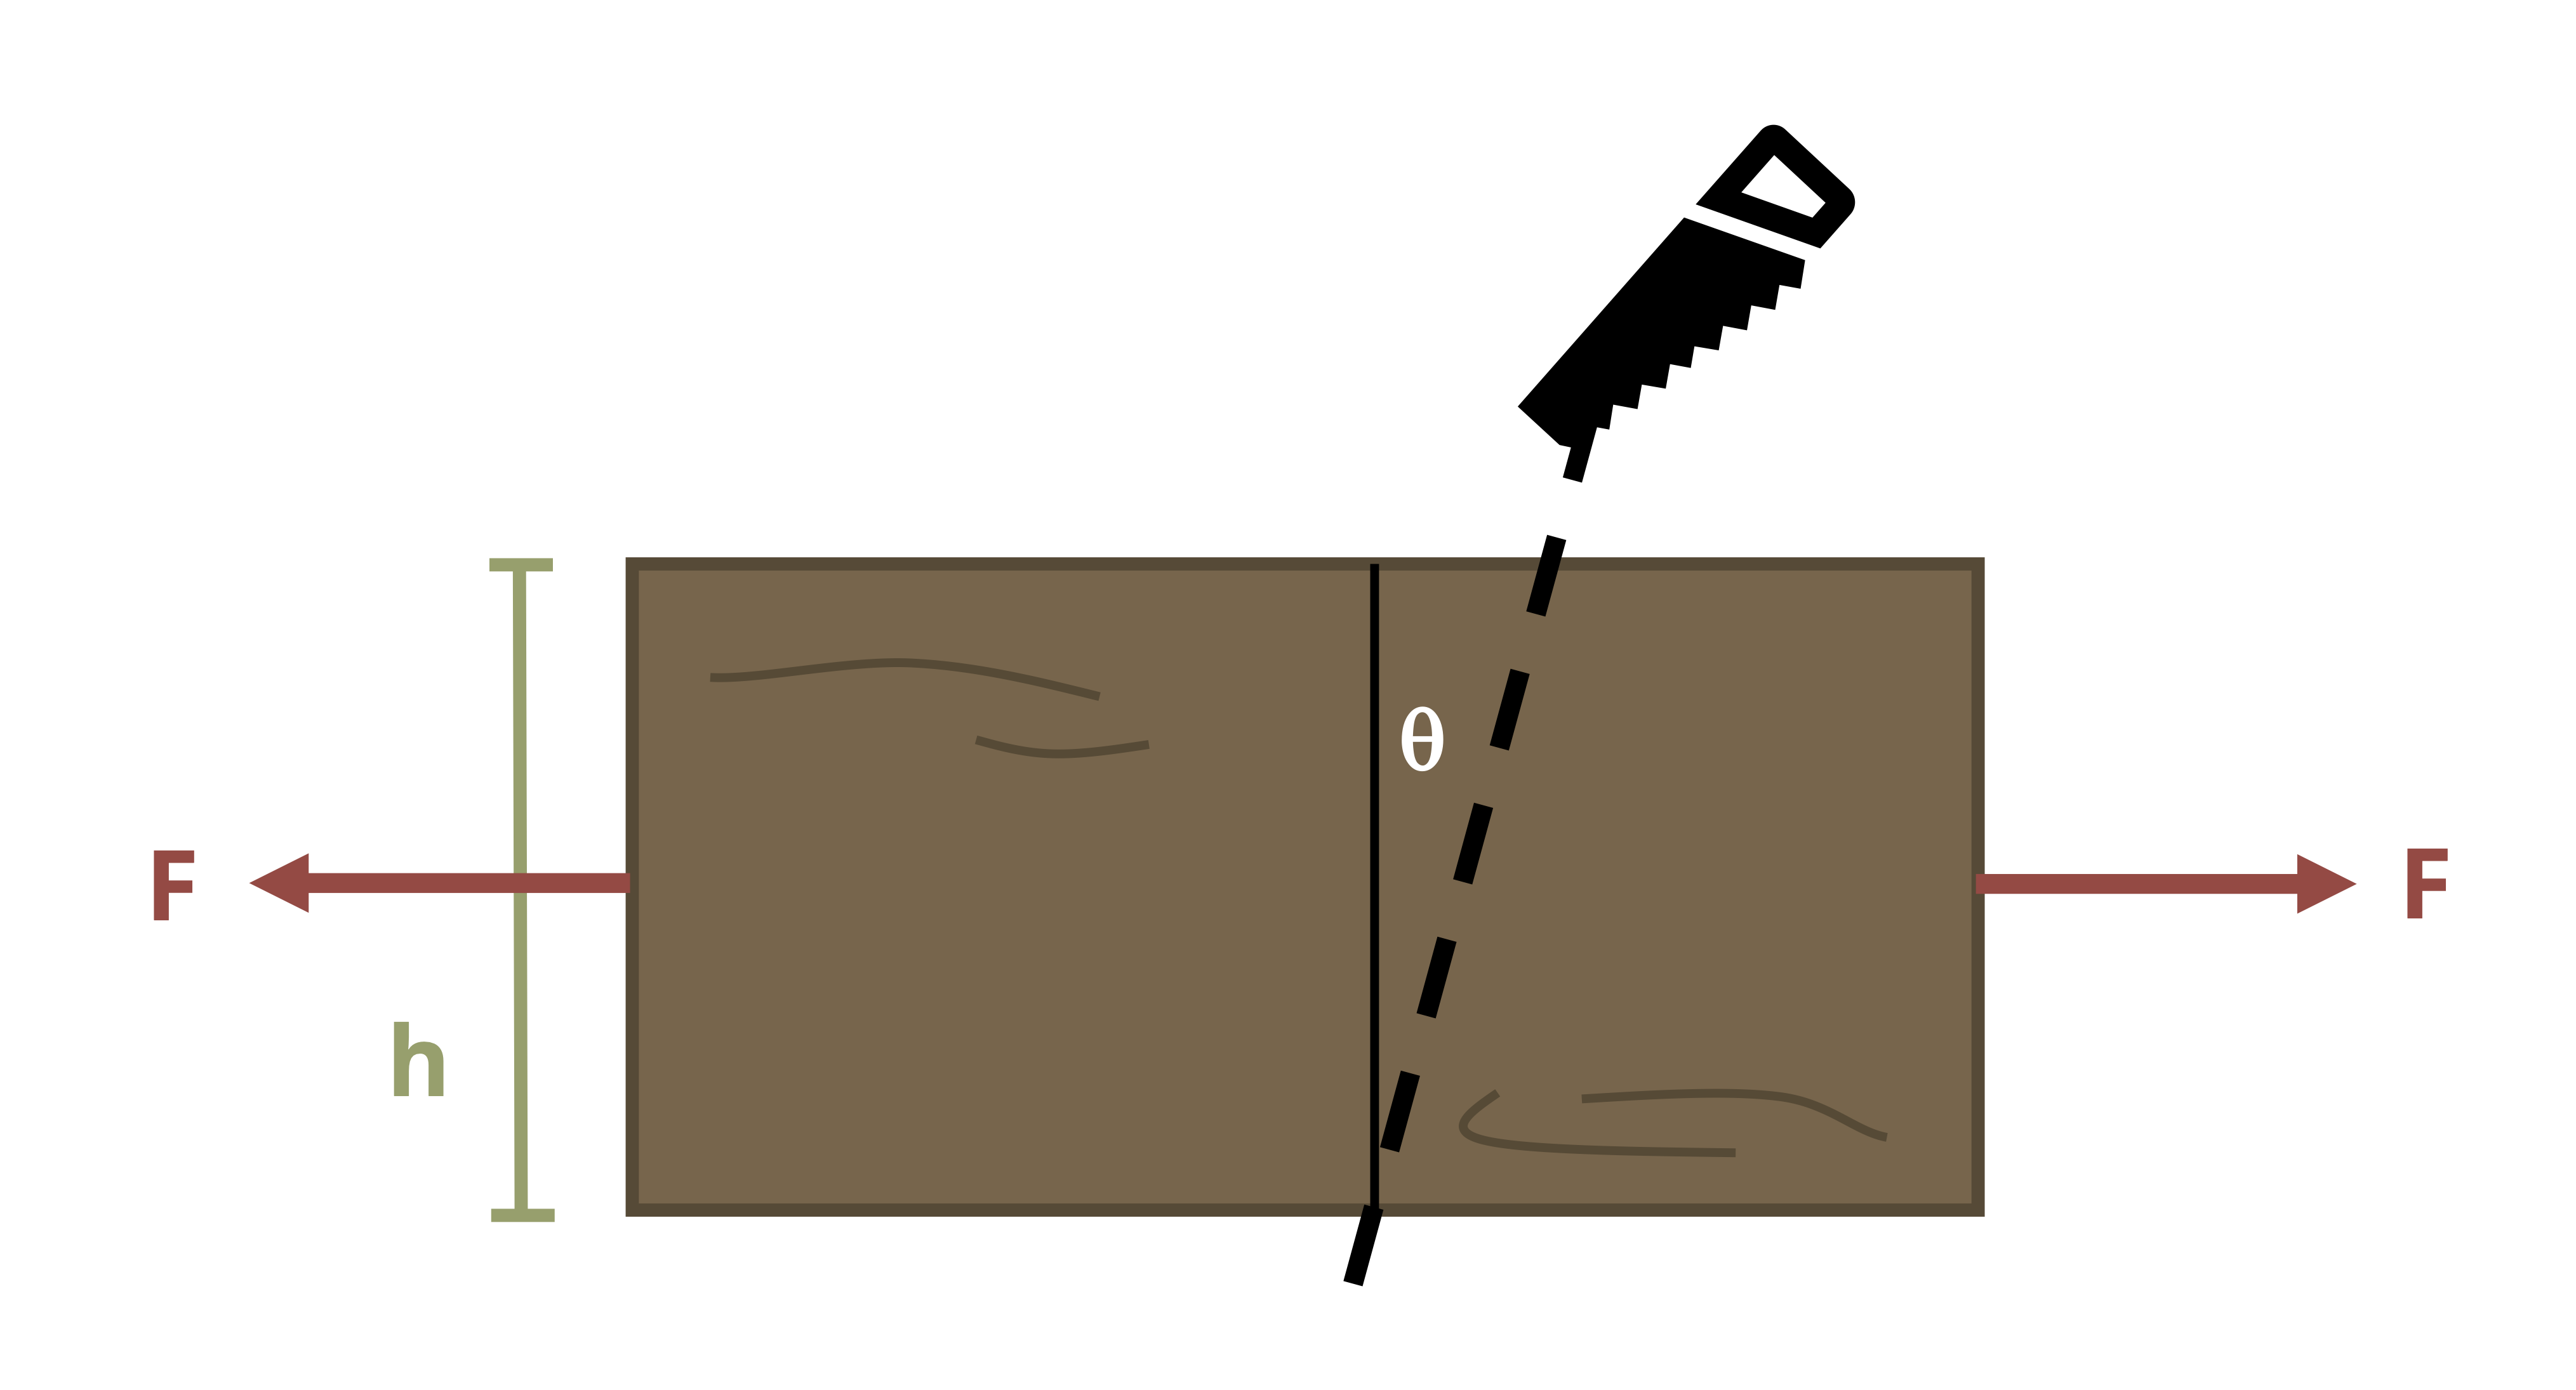
\includegraphics{images/156.png}

}

\caption{Figure 1: A two inch thick board is cut and then glued back
together.}

\end{figure}%

\begin{Shaded}
\begin{Highlighting}[]
\NormalTok{\#| standalone: true}
\NormalTok{\#| viewerHeight: 600}
\NormalTok{\#| components: [viewer]}

\NormalTok{from shiny import App, render, ui, reactive}
\NormalTok{import random}
\NormalTok{import asyncio}
\NormalTok{import io}
\NormalTok{import math}
\NormalTok{import string}
\NormalTok{from datetime import datetime}
\NormalTok{from pathlib import Path}

\NormalTok{def generate\_random\_letters(length):}
\NormalTok{    \# Generate a random string of letters of specified length}
\NormalTok{    return \textquotesingle{}\textquotesingle{}.join(random.choice(string.ascii\_lowercase) for \_ in range(length))  }

\NormalTok{problem\_ID="156"}
\NormalTok{F=reactive.Value("\_\_")}
\NormalTok{h=reactive.Value("\_\_")}
\NormalTok{Θ=reactive.Value("\_\_")}

\NormalTok{attempts=["Timestamp,Attempt,Answer,Feedback\textbackslash{}n"]}

\NormalTok{app\_ui = ui.page\_fluid(}
\NormalTok{    ui.markdown("**Please enter your ID number from your instructor and click to generate your problem**"),}
\NormalTok{    ui.input\_text("ID","", placeholder="Enter ID Number Here"),}
\NormalTok{    ui.input\_action\_button("generate\_problem", "Generate Problem", class\_="btn{-}primary"),}
\NormalTok{    ui.markdown("**Problem Statement**"),}
\NormalTok{    ui.output\_ui("ui\_problem\_statement"),}
\NormalTok{    ui.input\_text("answer","Your Answer in units of psi", placeholder="Please enter your answer"),}
\NormalTok{    ui.input\_action\_button("submit", "Submit Answer", class\_="btn{-}primary"),}
\NormalTok{    ui.download\_button("download", "Download File to Submit", class\_="btn{-}success"),}
\NormalTok{)}


\NormalTok{def server(input, output, session):}
\NormalTok{    \# Initialize a counter for attempts}
\NormalTok{    attempt\_counter = reactive.Value(0)}

\NormalTok{    @output}
\NormalTok{    @render.ui}
\NormalTok{    def ui\_problem\_statement():}
\NormalTok{        return[ui.markdown(f"A 2 inch thick board is cut and then glued back together along a line that is Θ = \{Θ()\} ° off the vertical as shown. If height h = \{h()\} in. and F = \{F()\} lb, determine the normal stress along the cut line.")]}
    
\NormalTok{    @reactive.Effect}
\NormalTok{    @reactive.event(input.generate\_problem)}
\NormalTok{    def randomize\_vars():}
\NormalTok{        random.seed(input.ID())}
\NormalTok{        F.set(random.randrange(2000, 6000, 100))}
\NormalTok{        h.set(random.randrange(50, 150, 1)/10)}
\NormalTok{        Θ.set(random.randrange(10, 20, 1))}
        

\NormalTok{    @reactive.Effect}
\NormalTok{    @reactive.event(input.submit)}
\NormalTok{    def \_():}
\NormalTok{        attempt\_counter.set(attempt\_counter() + 1)  \# Increment the attempt counter on each submission.}
        
\NormalTok{        instr= (F()/(2*h()))*(math.cos(math.radians(Θ()))**2)}
\NormalTok{        if math.isclose(float(input.answer()), instr, rel\_tol=0.01):}
\NormalTok{            check = "*Correct*"}
\NormalTok{            correct\_indicator = "JL"}
\NormalTok{        else:}
\NormalTok{            check = "*Not Correct.*"}
\NormalTok{            correct\_indicator = "JG"}

\NormalTok{        \# Generate random parts for the encoded attempt.}
\NormalTok{        random\_start = generate\_random\_letters(4)}
\NormalTok{        random\_middle = generate\_random\_letters(4)}
\NormalTok{        random\_end = generate\_random\_letters(4)}
\NormalTok{        encoded\_attempt = f"\{random\_start\}\{problem\_ID\}{-}\{random\_middle\}\{attempt\_counter()\}\{correct\_indicator\}{-}\{random\_end\}\{input.ID()\}"}

\NormalTok{        \# Store the most recent encoded attempt in a reactive value so it persists across submissions}
\NormalTok{        session.encoded\_attempt = reactive.Value(encoded\_attempt)}

\NormalTok{        \# Append the attempt data to the attempts list without the encoded attempt}
\NormalTok{        attempts.append(f"\{datetime.now()\}, \{attempt\_counter()\}, \{input.answer()\}, \{check\}\textbackslash{}n")}

\NormalTok{        \# Show feedback to the user.}
\NormalTok{        feedback = ui.markdown(f"Your answer of \{input.answer()\} is \{check\}.")}
\NormalTok{        m = ui.modal(}
\NormalTok{            feedback,}
\NormalTok{            title="Feedback",}
\NormalTok{            easy\_close=True}
\NormalTok{        )}
\NormalTok{        ui.modal\_show(m)}

\NormalTok{    @session.download(filename=lambda: f"Problem\_Log{-}\{problem\_ID\}{-}\{input.ID()\}.csv")}
\NormalTok{    async def download():}
\NormalTok{        \# Start the CSV with the encoded attempt (without label)}
\NormalTok{        final\_encoded = session.encoded\_attempt() if session.encoded\_attempt is not None else "No attempts"}
\NormalTok{        yield f"\{final\_encoded\}\textbackslash{}n\textbackslash{}n"}
        
\NormalTok{        \# Write the header for the remaining CSV data once}
\NormalTok{        yield "Timestamp,Attempt,Answer,Feedback\textbackslash{}n"}
        
\NormalTok{        \# Write the attempts data, ensure that the header from the attempts list is not written again}
\NormalTok{        for attempt in attempts[1:]:  \# Skip the first element which is the header}
\NormalTok{            await asyncio.sleep(0.25)  \# This delay may not be necessary; adjust as needed}
\NormalTok{            yield attempt}


\NormalTok{\# App installation}
\NormalTok{app = App(app\_ui, server)}
\end{Highlighting}
\end{Shaded}

\chapter*{Problem 4.35}\label{problem-4.35}
\addcontentsline{toc}{chapter}{Problem 4.35}

\markboth{Problem 4.35}{Problem 4.35}

This is a dynamic rendering of the problem with dynamic variables based
on the username entered.

\section*{Problem Image}\label{problem-image-6}
\addcontentsline{toc}{section}{Problem Image}

\markright{Problem Image}

\begin{figure}[H]

{\centering 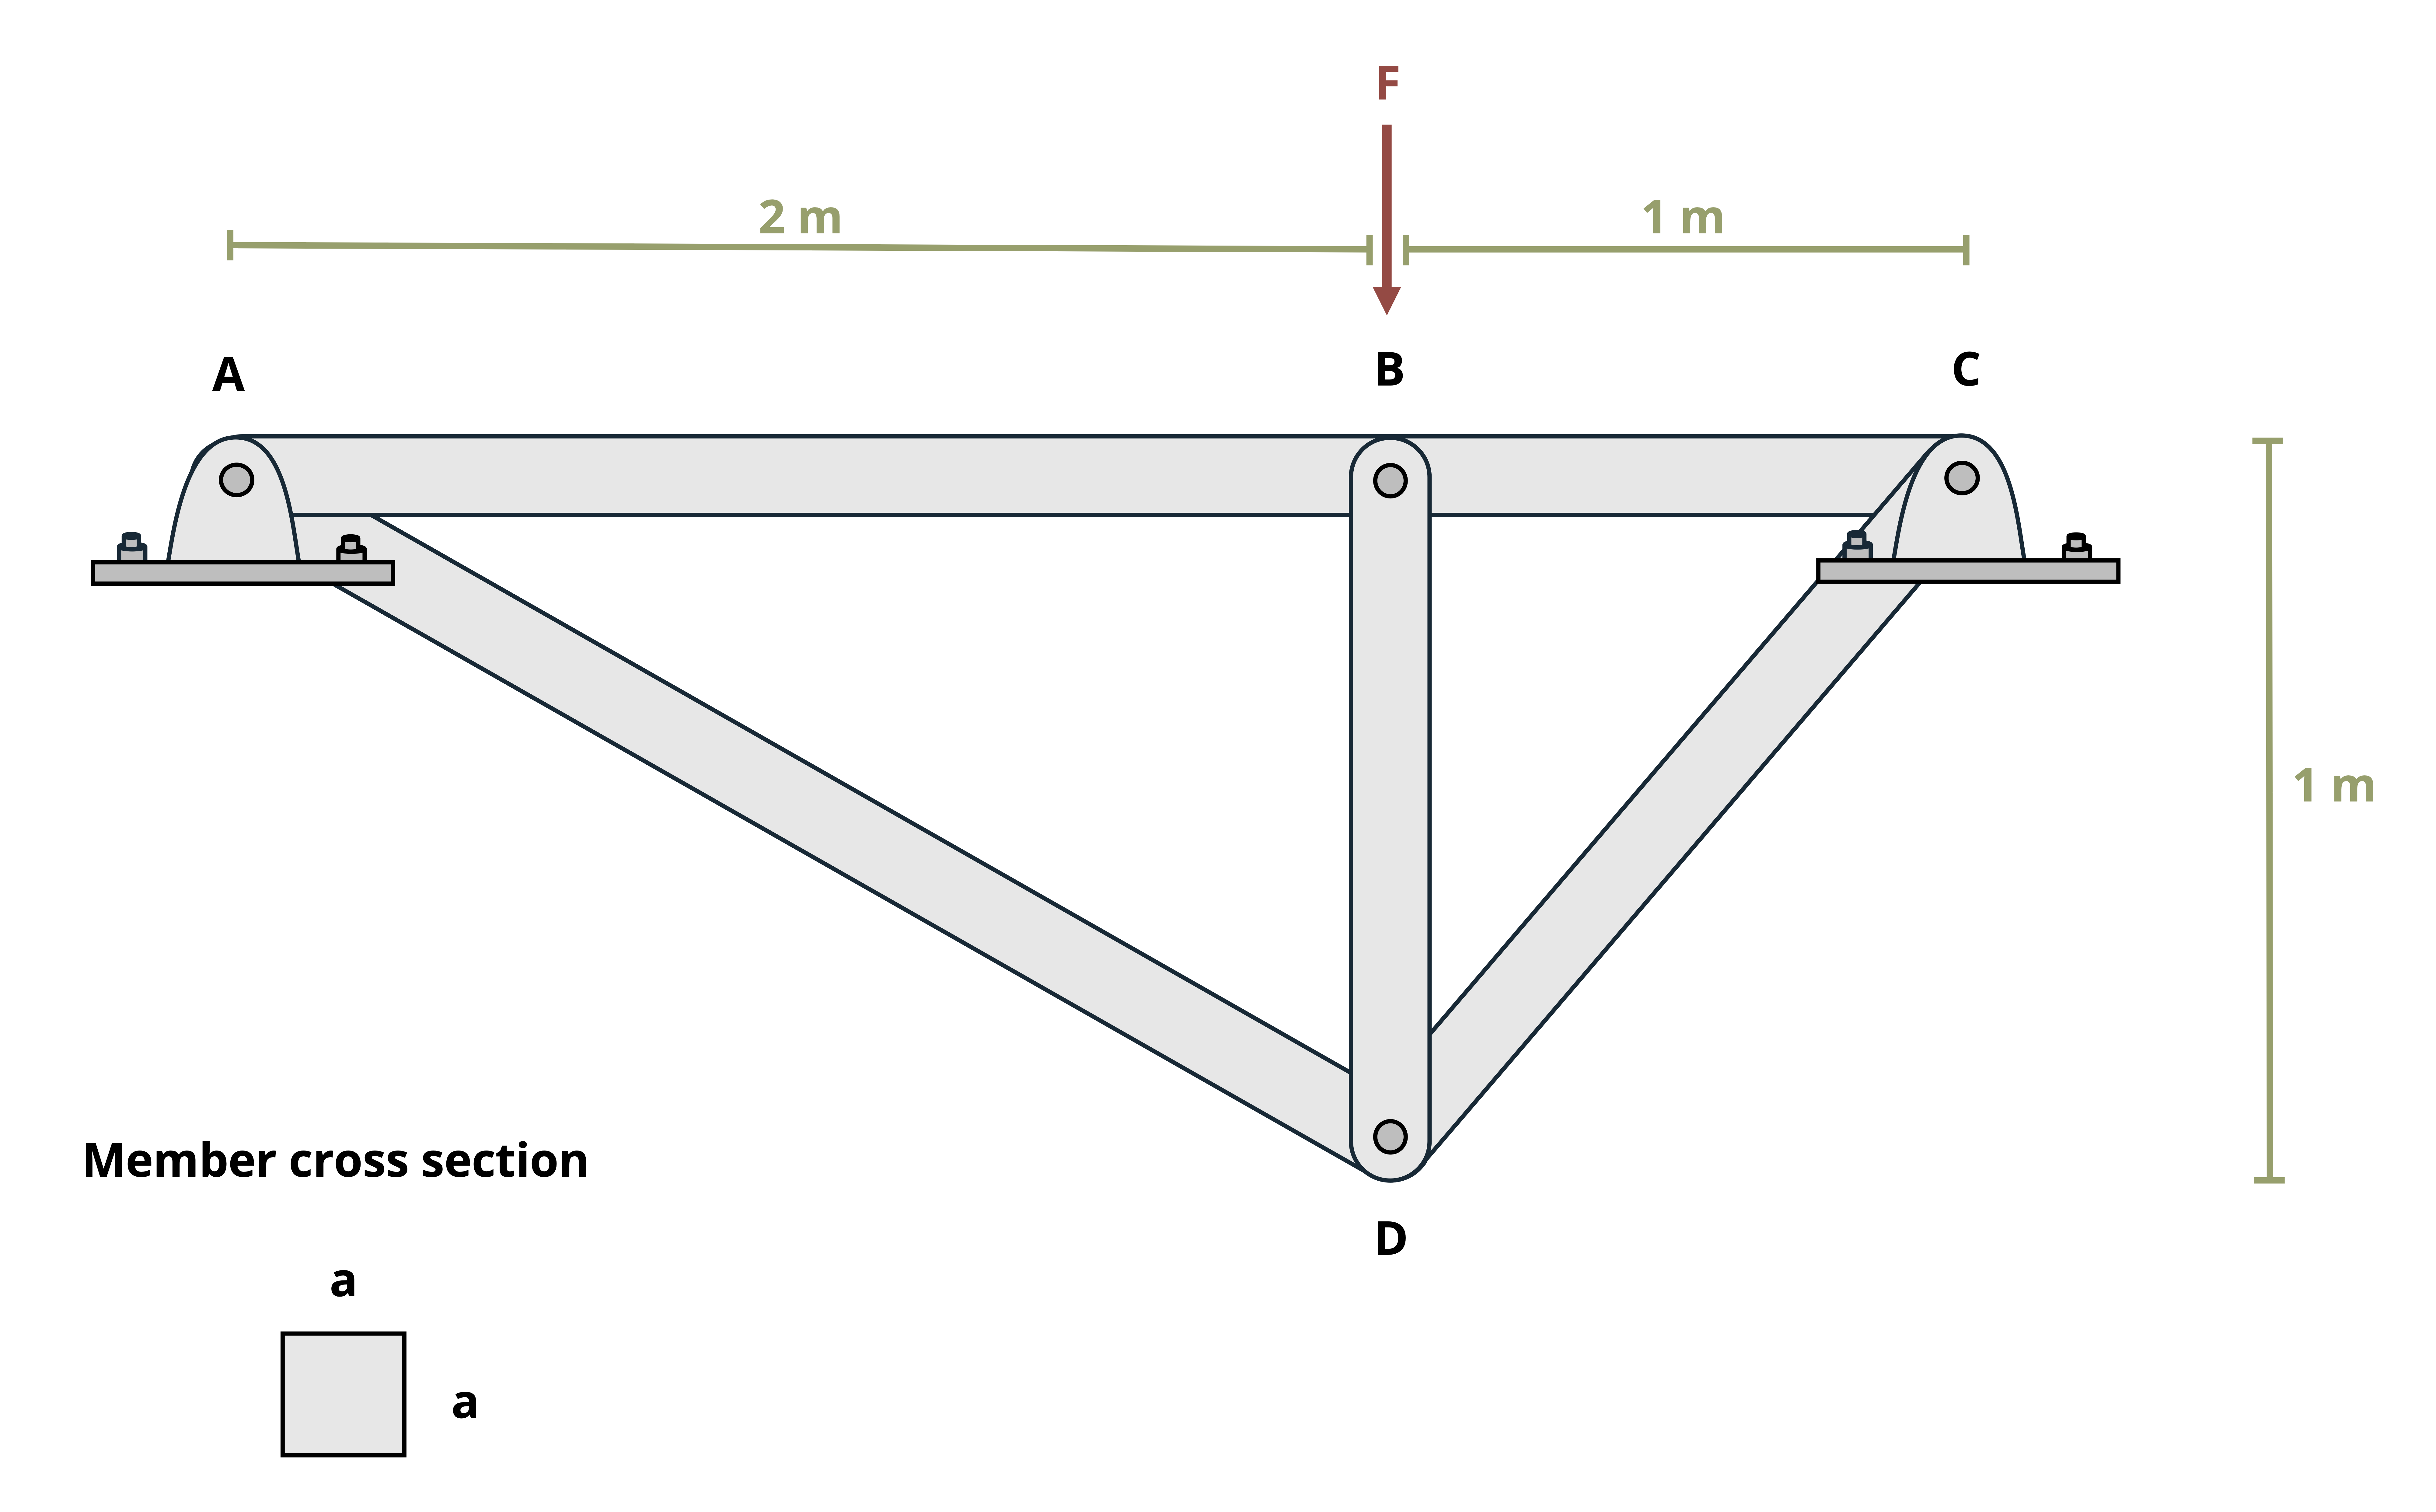
\includegraphics{images/157.png}

}

\caption{Figure 1: A small truss is constructed with solid square wood
members.}

\end{figure}%

\begin{Shaded}
\begin{Highlighting}[]
\NormalTok{\#| standalone: true}
\NormalTok{\#| viewerHeight: 600}
\NormalTok{\#| components: [viewer]}

\NormalTok{from shiny import App, render, ui, reactive}
\NormalTok{import random}
\NormalTok{import asyncio}
\NormalTok{import io}
\NormalTok{import math}
\NormalTok{import string}
\NormalTok{from datetime import datetime}
\NormalTok{from pathlib import Path}

\NormalTok{def generate\_random\_letters(length):}
\NormalTok{    \# Generate a random string of letters of specified length}
\NormalTok{    return \textquotesingle{}\textquotesingle{}.join(random.choice(string.ascii\_lowercase) for \_ in range(length))  }

\NormalTok{problem\_ID="157"}
\NormalTok{F=reactive.Value("\_\_")}
\NormalTok{FS=reactive.Value("\_\_")}
\NormalTok{σfail=reactive.Value("\_\_")}

\NormalTok{attempts=["Timestamp,Attempt,Answer,Feedback\textbackslash{}n"]}

\NormalTok{app\_ui = ui.page\_fluid(}
\NormalTok{    ui.markdown("**Please enter your ID number from your instructor and click to generate your problem**"),}
\NormalTok{    ui.input\_text("ID","", placeholder="Enter ID Number Here"),}
\NormalTok{    ui.input\_action\_button("generate\_problem", "Generate Problem", class\_="btn{-}primary"),}
\NormalTok{    ui.markdown("**Problem Statement**"),}
\NormalTok{    ui.output\_ui("ui\_problem\_statement"),}
\NormalTok{    ui.input\_text("answer","Your Answer in units of centimeters", placeholder="Please enter your answer"),}
\NormalTok{    ui.input\_action\_button("submit", "Submit Answer", class\_="btn{-}primary"),}
\NormalTok{    ui.download\_button("download", "Download File to Submit", class\_="btn{-}success"),}
\NormalTok{)}


\NormalTok{def server(input, output, session):}
\NormalTok{    \# Initialize a counter for attempts}
\NormalTok{    attempt\_counter = reactive.Value(0)}

\NormalTok{    @output}
\NormalTok{    @render.ui}
\NormalTok{    def ui\_problem\_statement():}
\NormalTok{        return[ui.markdown(f"A small truss is constructed with solid square wood members and subjected to a load of F = \{F()\} kN. Determine the minimum dimension, a, of the member so that the truss will have a factor of safety of \{FS()\}. All members have the same cross{-}section. The wood has a failure stress of σ\textless{}sub\textgreater{}fail\textless{}/sub\textgreater{} = \{σfail()\} MPa.")]}
    
\NormalTok{    @reactive.Effect}
\NormalTok{    @reactive.event(input.generate\_problem)}
\NormalTok{    def randomize\_vars():}
\NormalTok{        random.seed(input.ID())}
\NormalTok{        F.set(random.randrange(15, 50, 1))}
\NormalTok{        FS.set(random.randrange(15, 40, 1)/10)}
\NormalTok{        σfail.set(random.randrange(40, 60, 1))}
        

\NormalTok{    @reactive.Effect}
\NormalTok{    @reactive.event(input.submit)}
\NormalTok{    def \_():}
\NormalTok{        attempt\_counter.set(attempt\_counter() + 1)  \# Increment the attempt counter on each submission.}
    
\NormalTok{        dl = FS()*F()}
\NormalTok{        A = (dl/(σfail()*10**3))*100*100}
\NormalTok{        instr= math.sqrt(A)}
\NormalTok{        if math.isclose(float(input.answer()), instr, rel\_tol=0.01):}
\NormalTok{            check = "*Correct*"}
\NormalTok{            correct\_indicator = "JL"}
\NormalTok{        else:}
\NormalTok{            check = "*Not Correct.*"}
\NormalTok{            correct\_indicator = "JG"}

\NormalTok{        \# Generate random parts for the encoded attempt.}
\NormalTok{        random\_start = generate\_random\_letters(4)}
\NormalTok{        random\_middle = generate\_random\_letters(4)}
\NormalTok{        random\_end = generate\_random\_letters(4)}
\NormalTok{        encoded\_attempt = f"\{random\_start\}\{problem\_ID\}{-}\{random\_middle\}\{attempt\_counter()\}\{correct\_indicator\}{-}\{random\_end\}\{input.ID()\}"}

\NormalTok{        \# Store the most recent encoded attempt in a reactive value so it persists across submissions}
\NormalTok{        session.encoded\_attempt = reactive.Value(encoded\_attempt)}

\NormalTok{        \# Append the attempt data to the attempts list without the encoded attempt}
\NormalTok{        attempts.append(f"\{datetime.now()\}, \{attempt\_counter()\}, \{input.answer()\}, \{check\}\textbackslash{}n")}

\NormalTok{        \# Show feedback to the user.}
\NormalTok{        feedback = ui.markdown(f"Your answer of \{input.answer()\} is \{check\}.")}
\NormalTok{        m = ui.modal(}
\NormalTok{            feedback,}
\NormalTok{            title="Feedback",}
\NormalTok{            easy\_close=True}
\NormalTok{        )}
\NormalTok{        ui.modal\_show(m)}

\NormalTok{    @session.download(filename=lambda: f"Problem\_Log{-}\{problem\_ID\}{-}\{input.ID()\}.csv")}
\NormalTok{    async def download():}
\NormalTok{        \# Start the CSV with the encoded attempt (without label)}
\NormalTok{        final\_encoded = session.encoded\_attempt() if session.encoded\_attempt is not None else "No attempts"}
\NormalTok{        yield f"\{final\_encoded\}\textbackslash{}n\textbackslash{}n"}
        
\NormalTok{        \# Write the header for the remaining CSV data once}
\NormalTok{        yield "Timestamp,Attempt,Answer,Feedback\textbackslash{}n"}
        
\NormalTok{        \# Write the attempts data, ensure that the header from the attempts list is not written again}
\NormalTok{        for attempt in attempts[1:]:  \# Skip the first element which is the header}
\NormalTok{            await asyncio.sleep(0.25)  \# This delay may not be necessary; adjust as needed}
\NormalTok{            yield attempt}


\NormalTok{\# App installation}
\NormalTok{app = App(app\_ui, server)}
\end{Highlighting}
\end{Shaded}

\chapter*{Problem 2.21}\label{problem-2.21}
\addcontentsline{toc}{chapter}{Problem 2.21}

\markboth{Problem 2.21}{Problem 2.21}

This is a dynamic rendering of the problem with dynamic variables based
on the username entered.

\section*{Problem Image}\label{problem-image-7}
\addcontentsline{toc}{section}{Problem Image}

\markright{Problem Image}

\begin{figure}[H]

{\centering 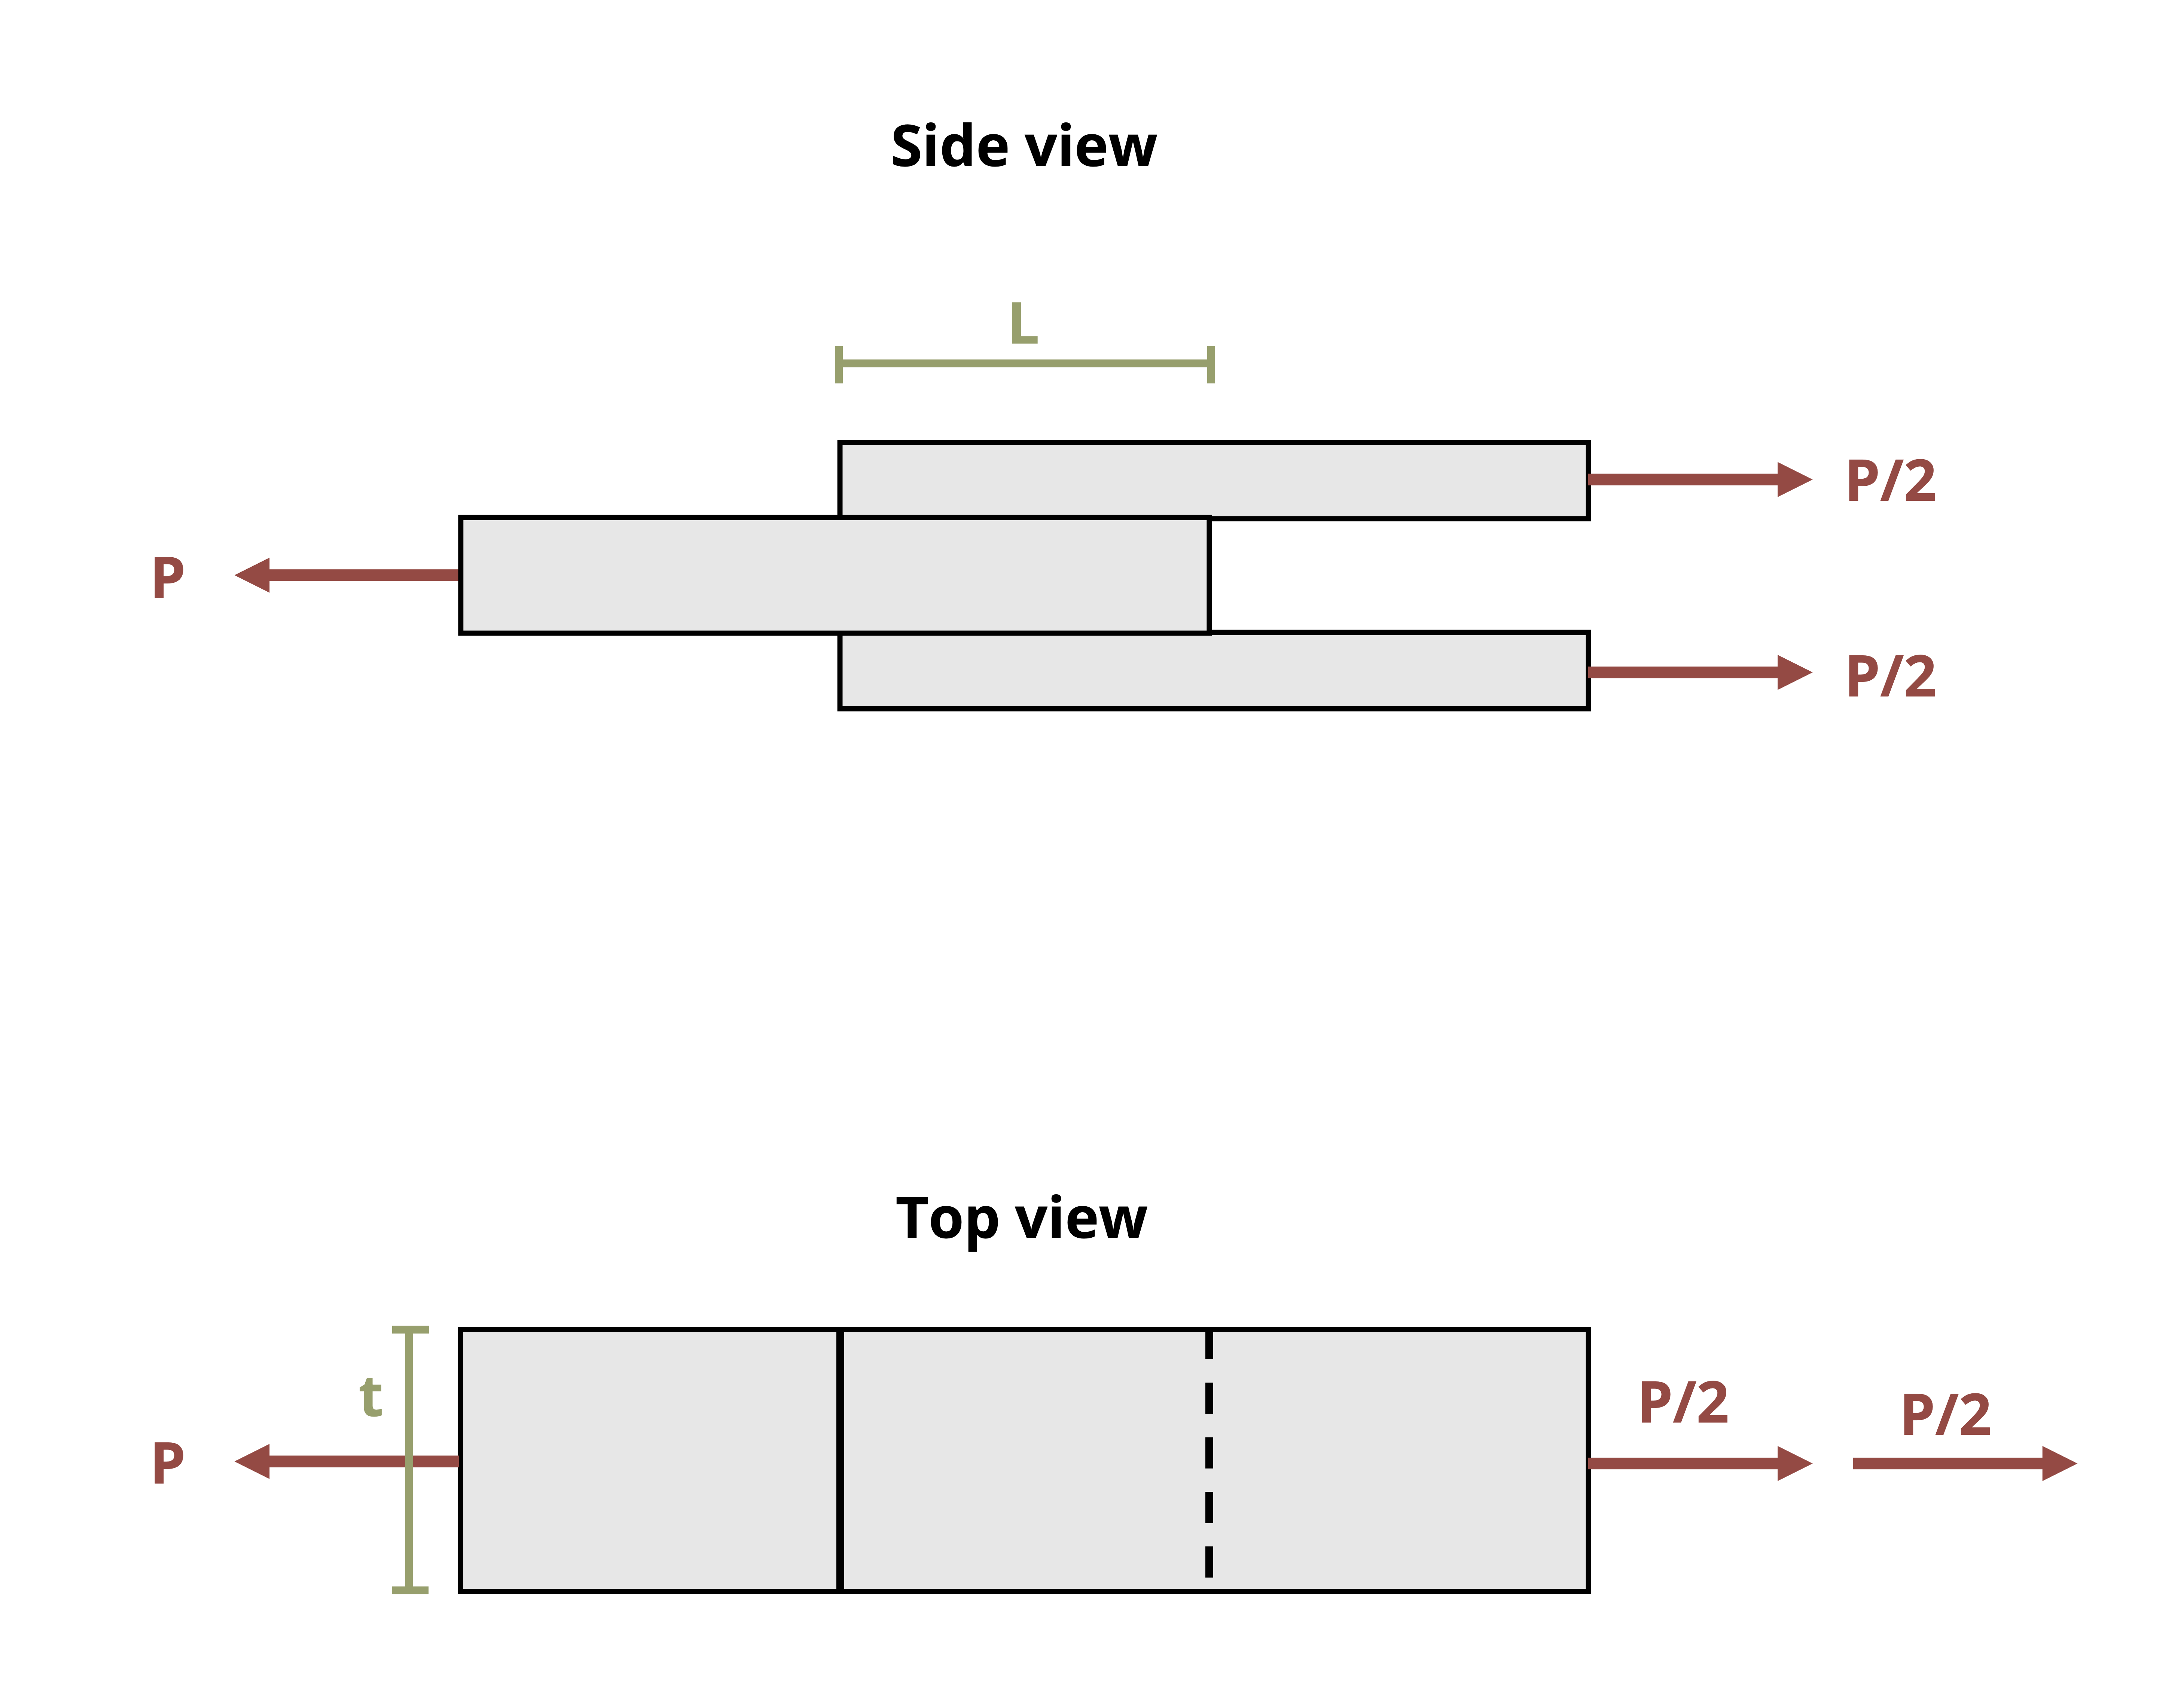
\includegraphics{images/164.png}

}

\caption{Figure 1: A double lap joint is glued together}

\end{figure}%

\begin{Shaded}
\begin{Highlighting}[]
\NormalTok{\#| standalone: true}
\NormalTok{\#| viewerHeight: 600}
\NormalTok{\#| components: [viewer]}

\NormalTok{from shiny import App, render, ui, reactive}
\NormalTok{import random}
\NormalTok{import asyncio}
\NormalTok{import io}
\NormalTok{import math}
\NormalTok{import string}
\NormalTok{from datetime import datetime}
\NormalTok{from pathlib import Path}

\NormalTok{def generate\_random\_letters(length):}
\NormalTok{    \# Generate a random string of letters of specified length}
\NormalTok{    return \textquotesingle{}\textquotesingle{}.join(random.choice(string.ascii\_lowercase) for \_ in range(length))  }

\NormalTok{problem\_ID="164"}
\NormalTok{τfail=reactive.Value("\_\_")}
\NormalTok{L=reactive.Value("\_\_")}
\NormalTok{t=reactive.Value("\_\_")}

\NormalTok{attempts=["Timestamp,Attempt,Answer,Feedback\textbackslash{}n"]}

\NormalTok{app\_ui = ui.page\_fluid(}
\NormalTok{    ui.markdown("**Please enter your ID number from your instructor and click to generate your problem**"),}
\NormalTok{    ui.input\_text("ID","", placeholder="Enter ID Number Here"),}
\NormalTok{    ui.input\_action\_button("generate\_problem", "Generate Problem", class\_="btn{-}primary"),}
\NormalTok{    ui.markdown("**Problem Statement**"),}
\NormalTok{    ui.output\_ui("ui\_problem\_statement"),}
\NormalTok{    ui.input\_text("answer","Your Answer in units of kips", placeholder="Please enter your answer"),}
\NormalTok{    ui.input\_action\_button("submit", "Submit Answer", class\_="btn{-}primary"),}
\NormalTok{    ui.download\_button("download", "Download File to Submit", class\_="btn{-}success"),}
\NormalTok{)}


\NormalTok{def server(input, output, session):}
\NormalTok{    \# Initialize a counter for attempts}
\NormalTok{    attempt\_counter = reactive.Value(0)}

\NormalTok{    @output}
\NormalTok{    @render.ui}
\NormalTok{    def ui\_problem\_statement():}
\NormalTok{        return[ui.markdown(f"A double lap joint is glued together using glue with a shear stress failure strength of \{τfail()\} psi. If dimensions L = \{L()\} in. and t = \{t()\} in., what is the maximum load P that the joint can withstand? Assume the load is evenly distributed across the joint on both sides.")]}
    
\NormalTok{    @reactive.Effect}
\NormalTok{    @reactive.event(input.generate\_problem)}
\NormalTok{    def randomize\_vars():}
\NormalTok{        random.seed(input.ID())}
\NormalTok{        τfail.set(random.randrange(7000, 9000, 100))}
\NormalTok{        L.set(random.randrange(40, 100, 1)/10)}
\NormalTok{        t.set(random.randrange(40, 100, 1)/10)}
        

\NormalTok{    @reactive.Effect}
\NormalTok{    @reactive.event(input.submit)}
\NormalTok{    def \_():}
\NormalTok{        attempt\_counter.set(attempt\_counter() + 1)  \# Increment the attempt counter on each submission.}
    
\NormalTok{        A = L()*t()*2}
\NormalTok{        instr= (τfail()*A)/1000}
\NormalTok{        if math.isclose(float(input.answer()), instr, rel\_tol=0.01):}
\NormalTok{            check = "*Correct*"}
\NormalTok{            correct\_indicator = "JL"}
\NormalTok{        else:}
\NormalTok{            check = "*Not Correct.*"}
\NormalTok{            correct\_indicator = "JG"}

\NormalTok{        \# Generate random parts for the encoded attempt.}
\NormalTok{        random\_start = generate\_random\_letters(4)}
\NormalTok{        random\_middle = generate\_random\_letters(4)}
\NormalTok{        random\_end = generate\_random\_letters(4)}
\NormalTok{        encoded\_attempt = f"\{random\_start\}\{problem\_ID\}{-}\{random\_middle\}\{attempt\_counter()\}\{correct\_indicator\}{-}\{random\_end\}\{input.ID()\}"}

\NormalTok{        \# Store the most recent encoded attempt in a reactive value so it persists across submissions}
\NormalTok{        session.encoded\_attempt = reactive.Value(encoded\_attempt)}

\NormalTok{        \# Append the attempt data to the attempts list without the encoded attempt}
\NormalTok{        attempts.append(f"\{datetime.now()\}, \{attempt\_counter()\}, \{input.answer()\}, \{check\}\textbackslash{}n")}

\NormalTok{        \# Show feedback to the user.}
\NormalTok{        feedback = ui.markdown(f"Your answer of \{input.answer()\} is \{check\}.")}
\NormalTok{        m = ui.modal(}
\NormalTok{            feedback,}
\NormalTok{            title="Feedback",}
\NormalTok{            easy\_close=True}
\NormalTok{        )}
\NormalTok{        ui.modal\_show(m)}

\NormalTok{    @session.download(filename=lambda: f"Problem\_Log{-}\{problem\_ID\}{-}\{input.ID()\}.csv")}
\NormalTok{    async def download():}
\NormalTok{        \# Start the CSV with the encoded attempt (without label)}
\NormalTok{        final\_encoded = session.encoded\_attempt() if session.encoded\_attempt is not None else "No attempts"}
\NormalTok{        yield f"\{final\_encoded\}\textbackslash{}n\textbackslash{}n"}
        
\NormalTok{        \# Write the header for the remaining CSV data once}
\NormalTok{        yield "Timestamp,Attempt,Answer,Feedback\textbackslash{}n"}
        
\NormalTok{        \# Write the attempts data, ensure that the header from the attempts list is not written again}
\NormalTok{        for attempt in attempts[1:]:  \# Skip the first element which is the header}
\NormalTok{            await asyncio.sleep(0.25)  \# This delay may not be necessary; adjust as needed}
\NormalTok{            yield attempt}


\NormalTok{\# App installation}
\NormalTok{app = App(app\_ui, server)}
\end{Highlighting}
\end{Shaded}

\chapter*{Problem 2.22}\label{problem-2.22}
\addcontentsline{toc}{chapter}{Problem 2.22}

\markboth{Problem 2.22}{Problem 2.22}

This is a dynamic rendering of the problem with dynamic variables based
on the username entered.

\section*{Problem Image}\label{problem-image-8}
\addcontentsline{toc}{section}{Problem Image}

\markright{Problem Image}

\begin{figure}[H]

{\centering 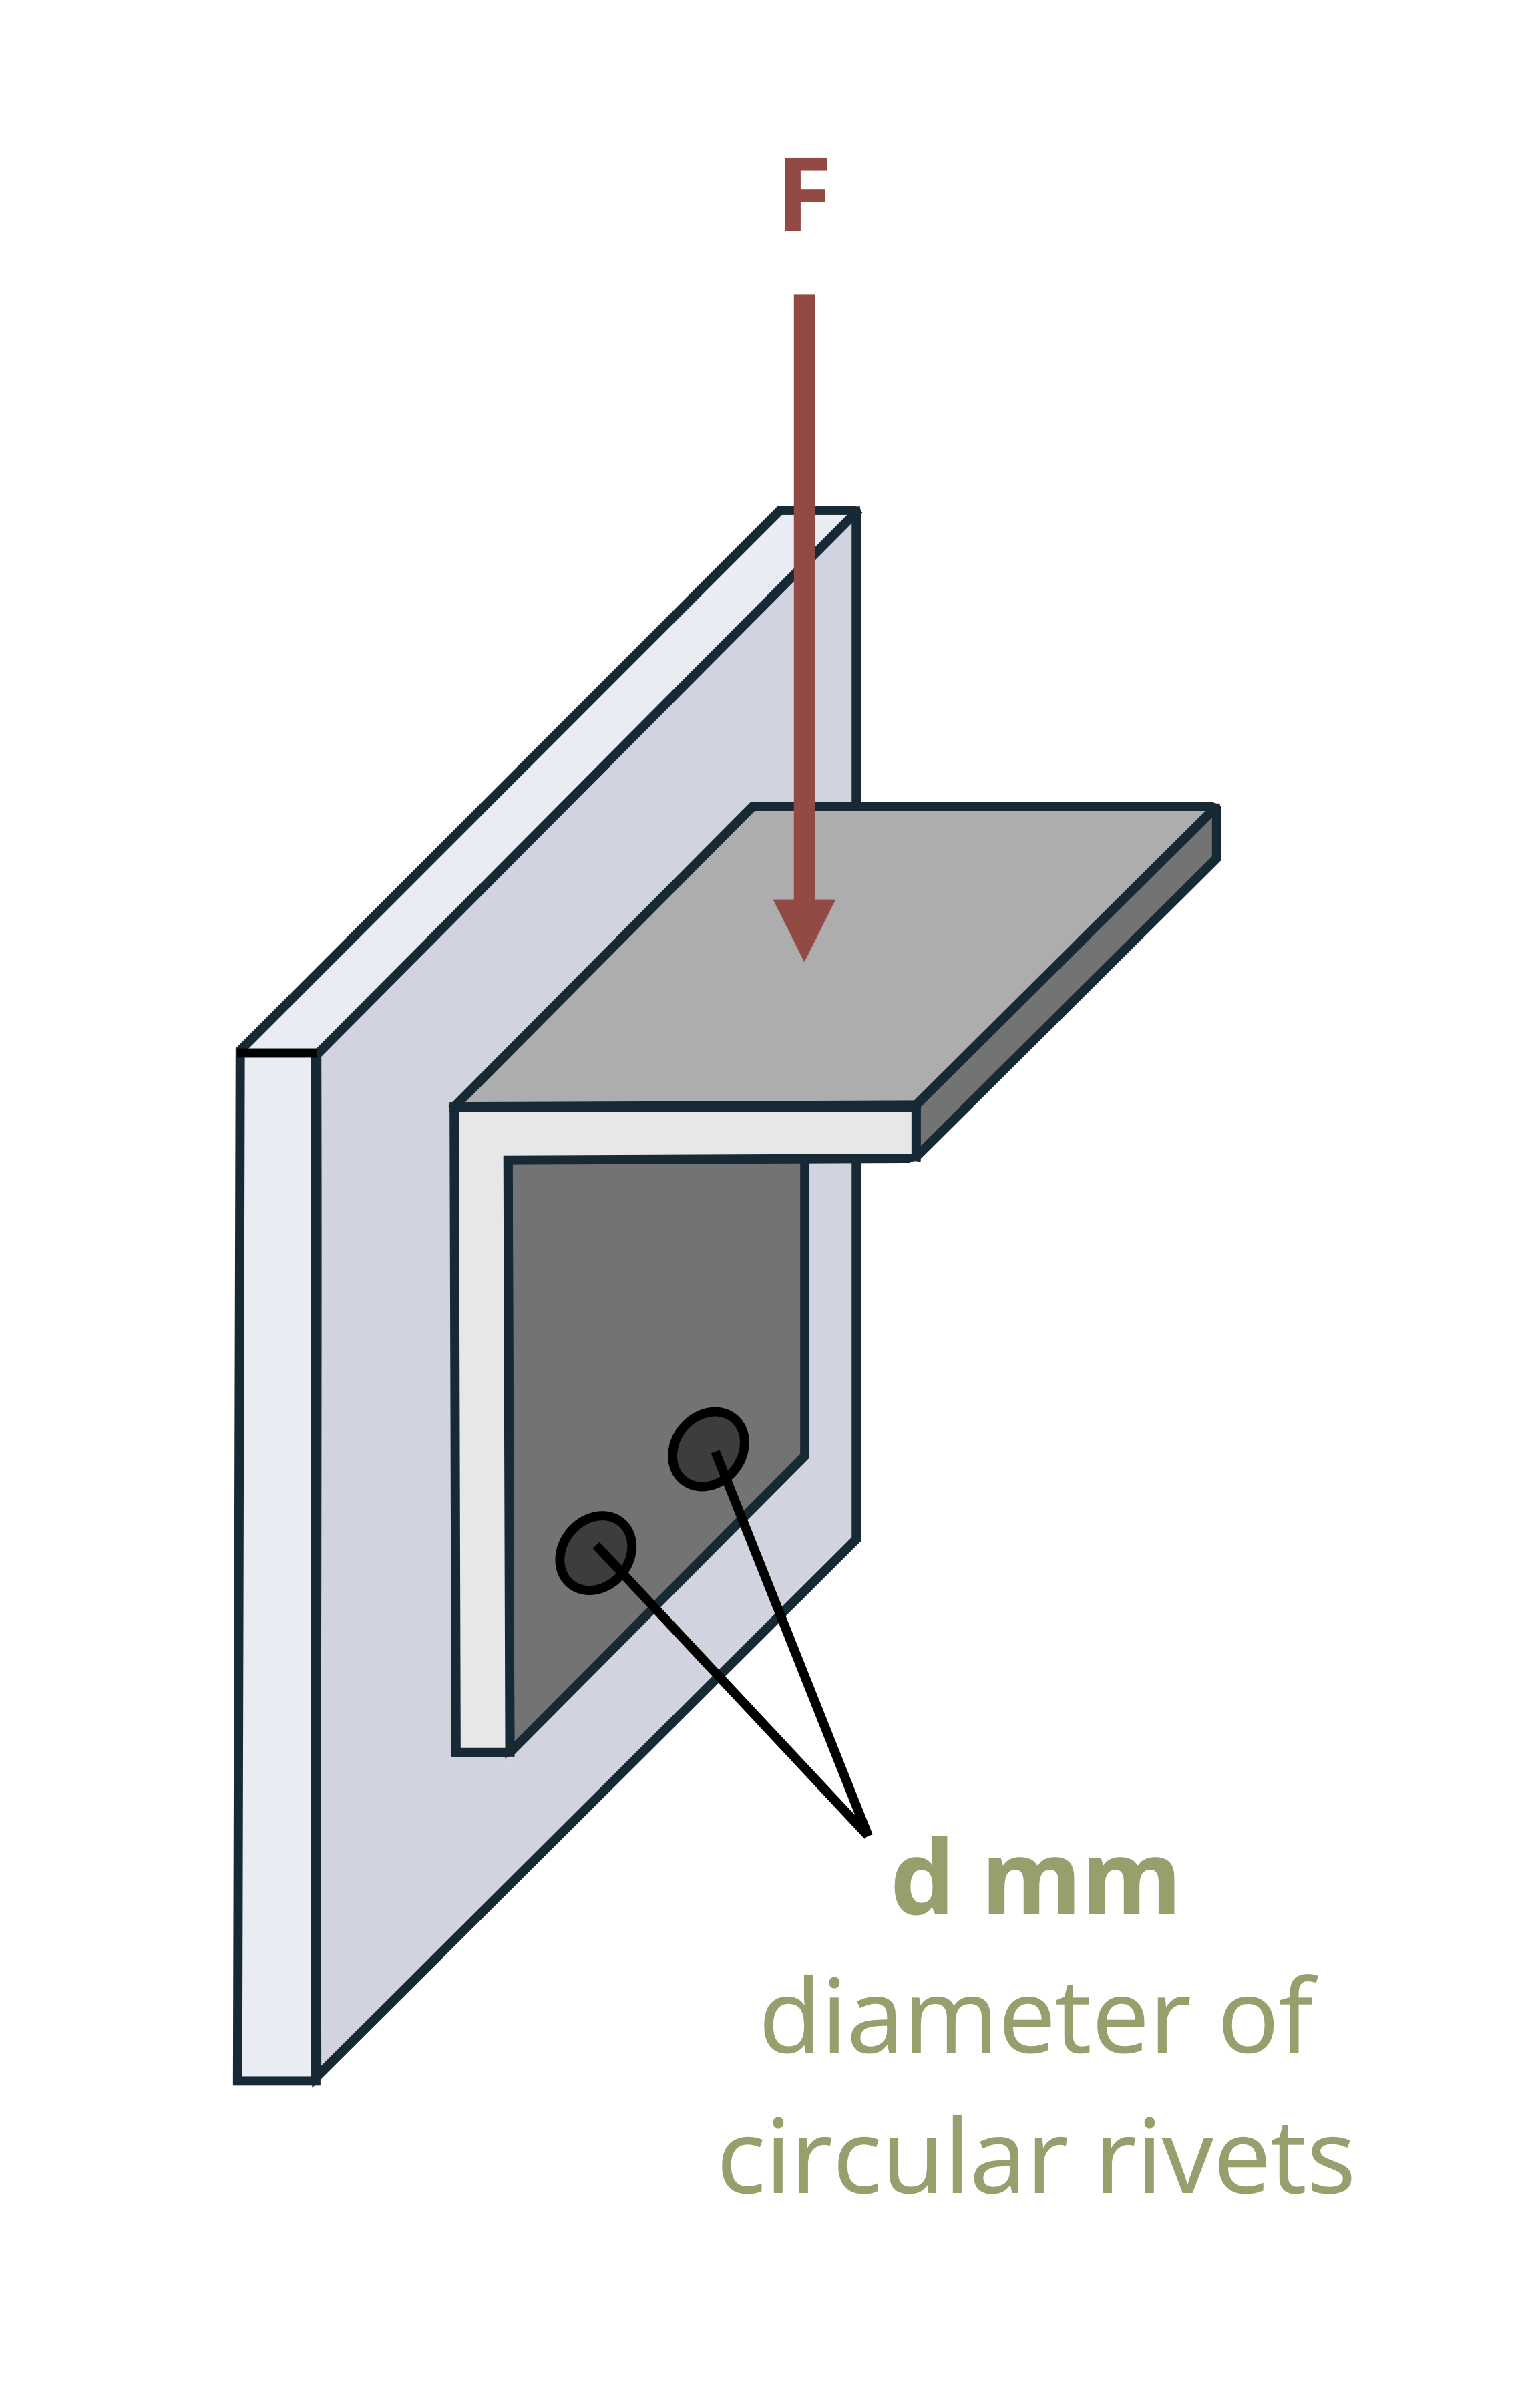
\includegraphics{images/165.png}

}

\caption{Figure 1: A bracket is attached to a wall with two circular
rivets.}

\end{figure}%

\begin{Shaded}
\begin{Highlighting}[]
\NormalTok{\#| standalone: true}
\NormalTok{\#| viewerHeight: 600}
\NormalTok{\#| components: [viewer]}

\NormalTok{from shiny import App, render, ui, reactive}
\NormalTok{import random}
\NormalTok{import asyncio}
\NormalTok{import io}
\NormalTok{import math}
\NormalTok{import string}
\NormalTok{from datetime import datetime}
\NormalTok{from pathlib import Path}

\NormalTok{def generate\_random\_letters(length):}
\NormalTok{    \# Generate a random string of letters of specified length}
\NormalTok{    return \textquotesingle{}\textquotesingle{}.join(random.choice(string.ascii\_lowercase) for \_ in range(length))}

\NormalTok{problem\_ID="165"}
\NormalTok{F=reactive.Value("\_\_")}
\NormalTok{d=reactive.Value("\_\_")}


\NormalTok{attempts=["Timestamp,Attempt,Answer,Feedback\textbackslash{}n"]}

\NormalTok{app\_ui = ui.page\_fluid(}
\NormalTok{    ui.markdown("**Please enter your ID number from your instructor and click to generate your problem**"),}
\NormalTok{    ui.input\_text("ID","", placeholder="Enter ID Number Here"),}
\NormalTok{    ui.input\_action\_button("generate\_problem", "Generate Problem", class\_="btn{-}primary"),}
\NormalTok{    ui.markdown("**Problem Statement**"),}
\NormalTok{    ui.output\_ui("ui\_problem\_statement"),}
\NormalTok{    ui.input\_text("answer","Your Answer in units of MPa", placeholder="Please enter your answer"),}
\NormalTok{    ui.input\_action\_button("submit", "Submit Answer", class\_="btn{-}primary"),}
\NormalTok{    ui.download\_button("download", "Download File to Submit", class\_="btn{-}success"),}
\NormalTok{)}


\NormalTok{def server(input, output, session):}
\NormalTok{    \# Initialize a counter for attempts}
\NormalTok{    attempt\_counter = reactive.Value(0)}

\NormalTok{    @output}
\NormalTok{    @render.ui}
\NormalTok{    def ui\_problem\_statement():}
\NormalTok{        return[ui.markdown(f"A bracket is attached to a wall with two circular rivets of diameter d = \{d()\} mm. A load F = \{F()\} kN is applied in the center of the bracket. Assuming the load is split evenly between the two rivits, determine the shear stress in each rivet. ")]}
    
\NormalTok{    @reactive.Effect}
\NormalTok{    @reactive.event(input.generate\_problem)}
\NormalTok{    def randomize\_vars():}
\NormalTok{        random.seed(input.ID())}
\NormalTok{        F.set(random.randrange(30, 100, 1))}
\NormalTok{        d.set(random.randrange(10, 40, 1))}
        

\NormalTok{    @reactive.Effect}
\NormalTok{    @reactive.event(input.submit)}
\NormalTok{    def \_():}
\NormalTok{        attempt\_counter.set(attempt\_counter() + 1)  \# Increment the attempt counter on each submission.  }
      
\NormalTok{        A = math.pi*(d()/(1000*2))**2}
\NormalTok{        instr= ((F()/2)/A)/1000}
\NormalTok{        if math.isclose(float(input.answer()), instr, rel\_tol=0.01):}
\NormalTok{            check = "*Correct*"}
\NormalTok{            correct\_indicator = "JL"}
\NormalTok{        else:}
\NormalTok{            check = "*Not Correct.*"}
\NormalTok{            correct\_indicator = "JG"}

\NormalTok{        \# Generate random parts for the encoded attempt.}
\NormalTok{        random\_start = generate\_random\_letters(4)}
\NormalTok{        random\_middle = generate\_random\_letters(4)}
\NormalTok{        random\_end = generate\_random\_letters(4)}
\NormalTok{        encoded\_attempt = f"\{random\_start\}\{problem\_ID\}{-}\{random\_middle\}\{attempt\_counter()\}\{correct\_indicator\}{-}\{random\_end\}\{input.ID()\}"}

\NormalTok{        \# Store the most recent encoded attempt in a reactive value so it persists across submissions}
\NormalTok{        session.encoded\_attempt = reactive.Value(encoded\_attempt)}

\NormalTok{        \# Append the attempt data to the attempts list without the encoded attempt}
\NormalTok{        attempts.append(f"\{datetime.now()\}, \{attempt\_counter()\}, \{input.answer()\}, \{check\}\textbackslash{}n")}

\NormalTok{        \# Show feedback to the user.}
\NormalTok{        feedback = ui.markdown(f"Your answer of \{input.answer()\} is \{check\}.")}
\NormalTok{        m = ui.modal(}
\NormalTok{            feedback,}
\NormalTok{            title="Feedback",}
\NormalTok{            easy\_close=True}
\NormalTok{        )}
\NormalTok{        ui.modal\_show(m)}

\NormalTok{    @session.download(filename=lambda: f"Problem\_Log{-}\{problem\_ID\}{-}\{input.ID()\}.csv")}
\NormalTok{    async def download():}
\NormalTok{        \# Start the CSV with the encoded attempt (without label)}
\NormalTok{        final\_encoded = session.encoded\_attempt() if session.encoded\_attempt is not None else "No attempts"}
\NormalTok{        yield f"\{final\_encoded\}\textbackslash{}n\textbackslash{}n"}
        
\NormalTok{        \# Write the header for the remaining CSV data once}
\NormalTok{        yield "Timestamp,Attempt,Answer,Feedback\textbackslash{}n"}
        
\NormalTok{        \# Write the attempts data, ensure that the header from the attempts list is not written again}
\NormalTok{        for attempt in attempts[1:]:  \# Skip the first element which is the header}
\NormalTok{            await asyncio.sleep(0.25)  \# This delay may not be necessary; adjust as needed}
\NormalTok{            yield attempt}


\NormalTok{\# App installation}
\NormalTok{app = App(app\_ui, server)}
\end{Highlighting}
\end{Shaded}

\chapter*{Problem 2.38}\label{problem-2.38}
\addcontentsline{toc}{chapter}{Problem 2.38}

\markboth{Problem 2.38}{Problem 2.38}

This is a dynamic rendering of the problem with dynamic variables based
on the username entered.

\section*{Problem Image}\label{problem-image-9}
\addcontentsline{toc}{section}{Problem Image}

\markright{Problem Image}

\begin{figure}[H]

{\centering 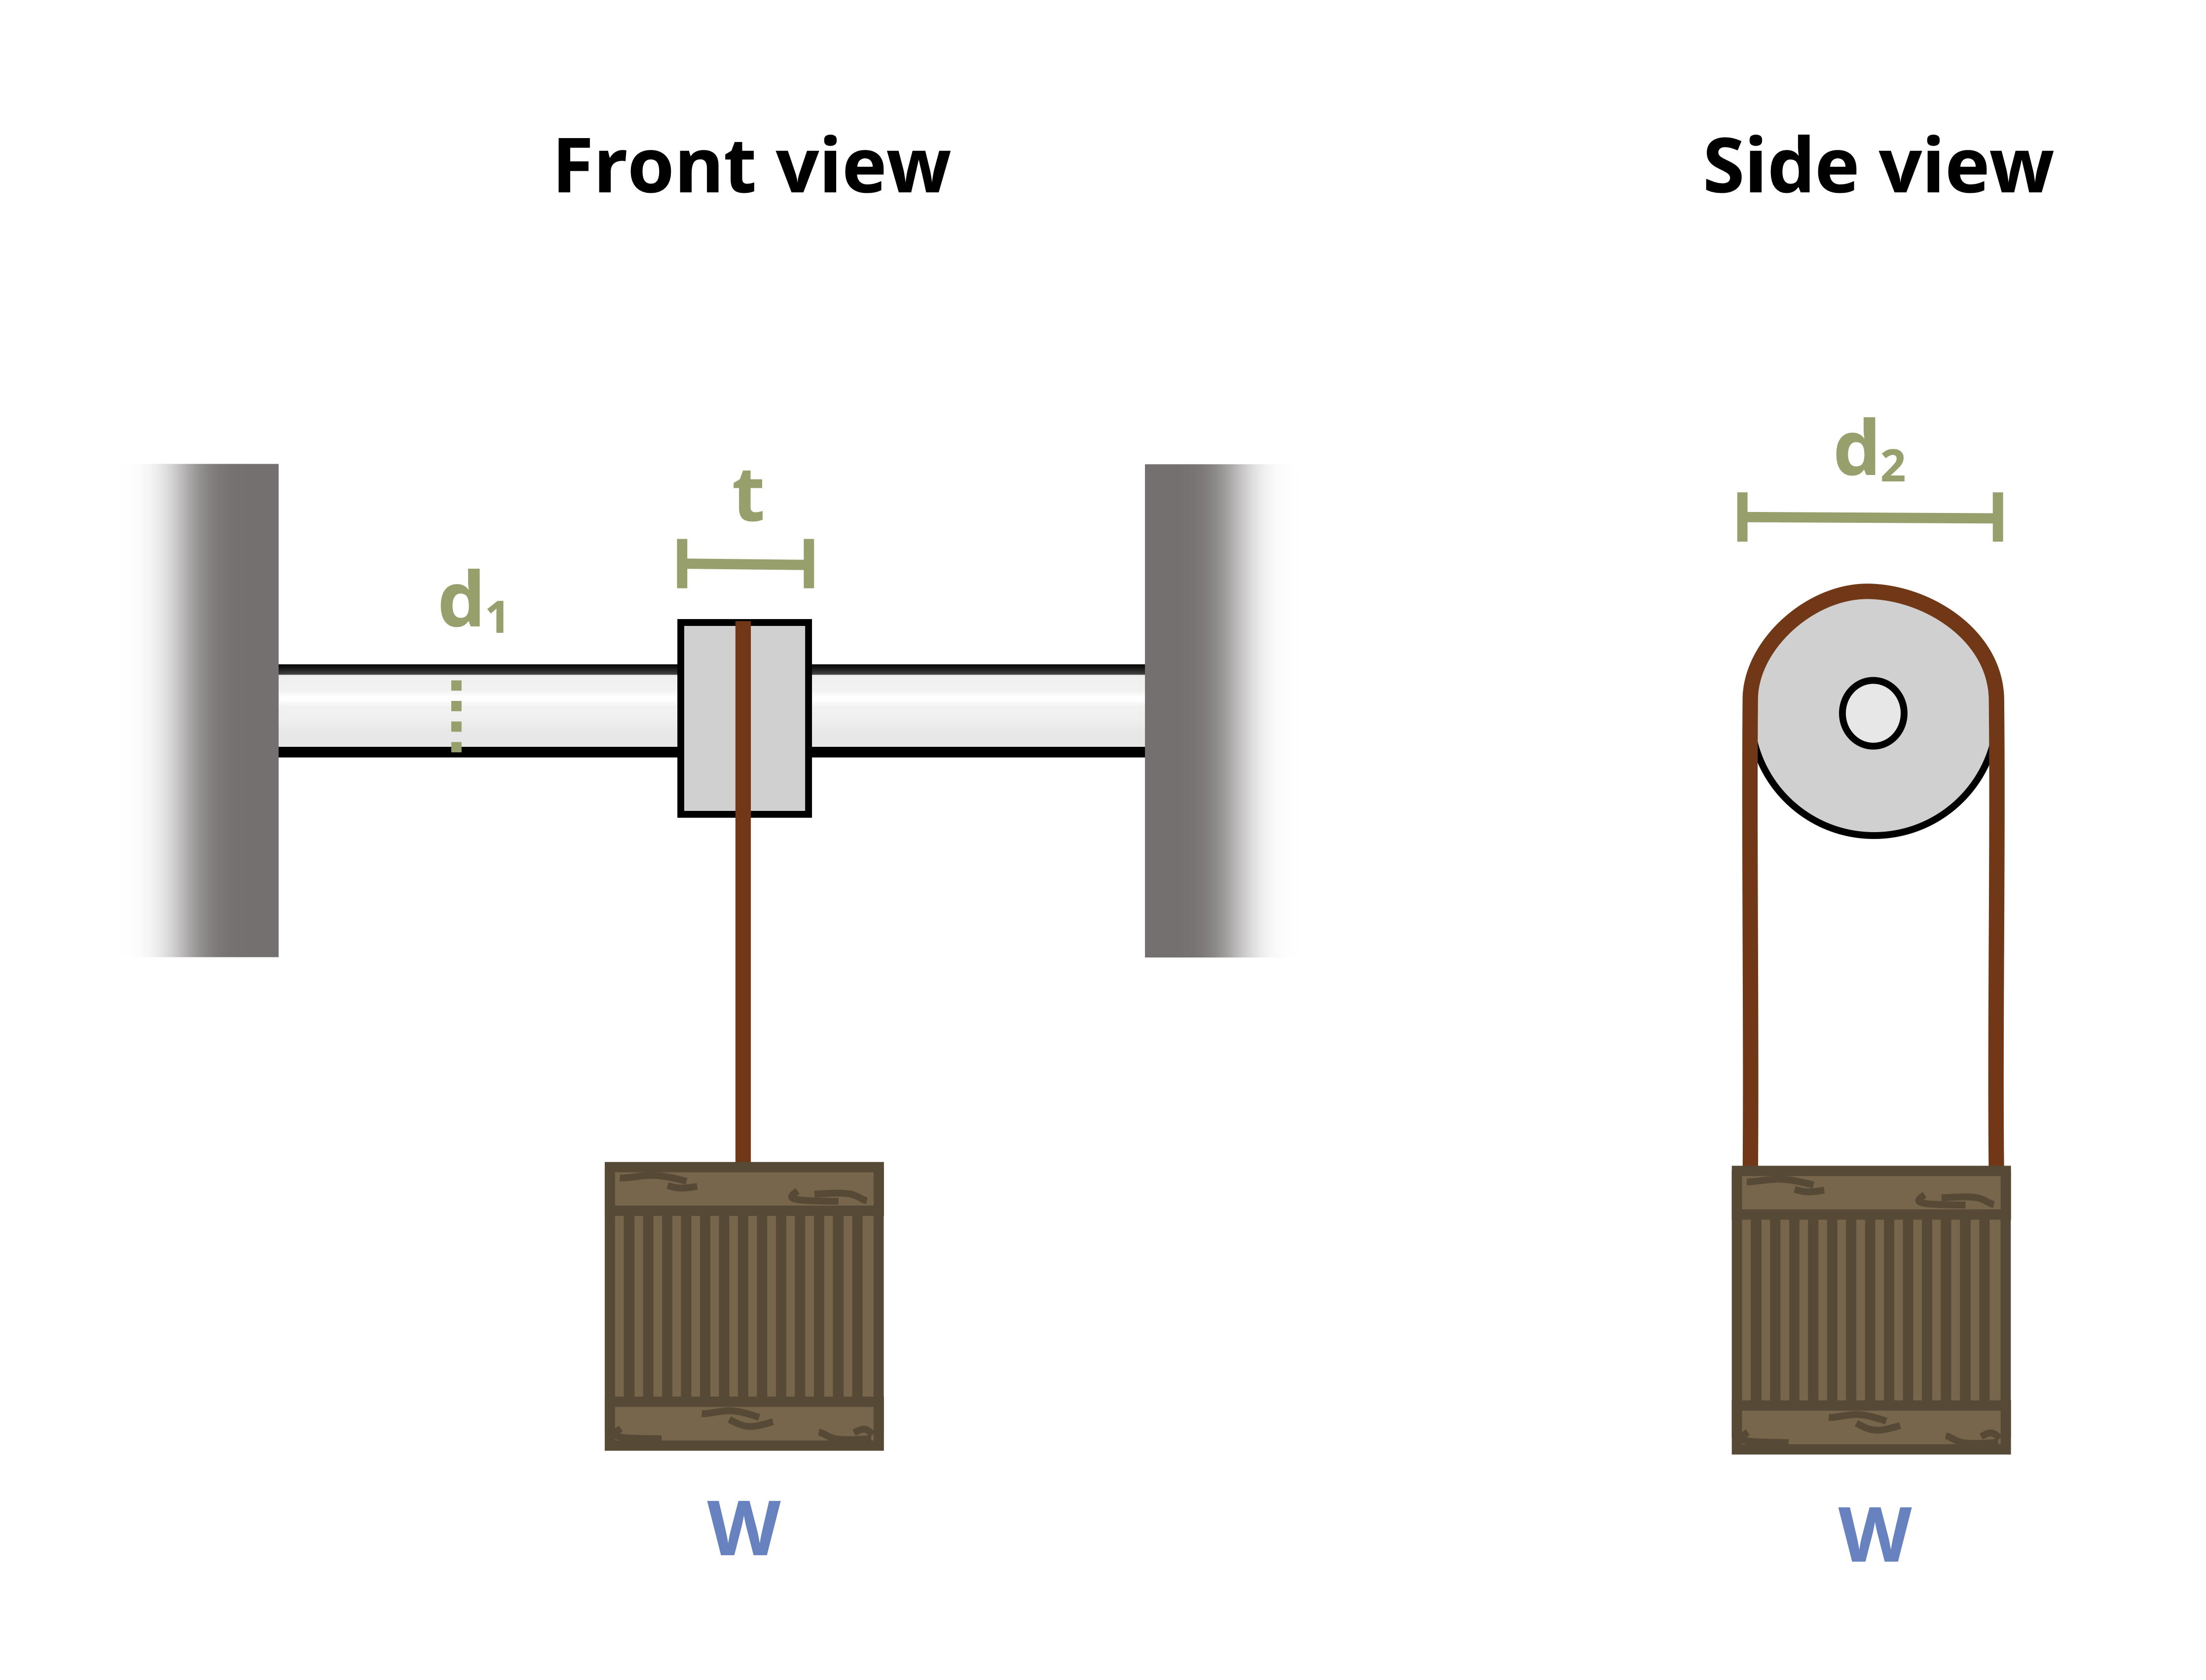
\includegraphics{images/166.png}

}

\caption{Figure 1: A crate is hung on a circular solid metal rod.}

\end{figure}%

\begin{Shaded}
\begin{Highlighting}[]
\NormalTok{\#| standalone: true}
\NormalTok{\#| viewerHeight: 600}
\NormalTok{\#| components: [viewer]}
\NormalTok{from shiny import App, render, ui, reactive}
\NormalTok{import random}
\NormalTok{import asyncio}
\NormalTok{import io}
\NormalTok{import math}
\NormalTok{import string}
\NormalTok{from datetime import datetime}
\NormalTok{from pathlib import Path}

\NormalTok{def generate\_random\_letters(length):}
\NormalTok{    \# Generate a random string of letters of specified length}
\NormalTok{    return \textquotesingle{}\textquotesingle{}.join(random.choice(string.ascii\_lowercase) for \_ in range(length))}

\NormalTok{problem\_ID="166"}
\NormalTok{W=reactive.Value("\_\_")}
\NormalTok{d1=reactive.Value("\_\_")}
\NormalTok{d2=reactive.Value("\_\_")}
\NormalTok{t=reactive.Value("\_\_")}
\NormalTok{attempts=["Timestamp,Attempt,Answer,Feedback\textbackslash{}n"]}

\NormalTok{app\_ui = ui.page\_fluid(}
\NormalTok{    ui.markdown("**Please enter your ID number from your instructor and click to generate your problem**"),}
\NormalTok{    ui.input\_text("ID","", placeholder="Enter ID Number Here"),}
\NormalTok{    ui.input\_action\_button("generate\_problem", "Generate Problem", class\_="btn{-}primary"),}
\NormalTok{    ui.markdown("**Problem Statement**"),}
\NormalTok{    ui.output\_ui("ui\_problem\_statement"),}
\NormalTok{    ui.input\_text("answer","Your Answer in units of ksi", placeholder="Please enter your answer"),}
\NormalTok{    ui.input\_action\_button("submit", "Submit Answer", class\_="btn{-}primary"),}
\NormalTok{    ui.download\_button("download", "Download File to Submit", class\_="btn{-}success"),}
\NormalTok{)}


\NormalTok{def server(input, output, session):}
\NormalTok{    \# Initialize a counter for attempts}
\NormalTok{    attempt\_counter = reactive.Value(0)}
    
\NormalTok{    @output}
\NormalTok{    @render.ui}
\NormalTok{    def ui\_problem\_statement():}
\NormalTok{        return[ui.markdown(f"A crate of weight \{W()\} = lb hangs from a solid circular metal rod of diameter \{d1()\} = in.. The cable is wrapped around a support collar of diameter \{d2()\} = in. and thickness \{t()\} = in. to evenly distribute the cable load. What is the bearing stress on the support collar due to the rod? ")]}
    
\NormalTok{    @reactive.Effect}
\NormalTok{    @reactive.event(input.generate\_problem)}
\NormalTok{    def randomize\_vars():}
\NormalTok{        random.seed(input.ID())}
\NormalTok{        W.set(random.randrange(4000, 9000, 100))}
\NormalTok{        d1.set(random.randrange(5, 30, 1)/10)}
\NormalTok{        d2.set(d1()*3)}
\NormalTok{        t.set(d1()*2)}
\NormalTok{    @reactive.Effect}
\NormalTok{    @reactive.event(input.submit)}
\NormalTok{    def \_():}
        
\NormalTok{        instr= W()/(d1()*t()*1000)}
        
\NormalTok{        if math.isclose(float(input.answer()), instr, rel\_tol=0.01):}
\NormalTok{            check = "*Correct*"}
\NormalTok{            correct\_indicator = "JL"}
\NormalTok{        else:}
\NormalTok{            check = "*Not Correct.*"}
\NormalTok{            correct\_indicator = "JG"}

\NormalTok{        \# Generate random parts for the encoded attempt.}
\NormalTok{        random\_start = generate\_random\_letters(4)}
\NormalTok{        random\_middle = generate\_random\_letters(4)}
\NormalTok{        random\_end = generate\_random\_letters(4)}
\NormalTok{        encoded\_attempt = f"\{random\_start\}\{problem\_ID\}{-}\{random\_middle\}\{attempt\_counter()\}\{correct\_indicator\}{-}\{random\_end\}\{input.ID()\}"}

\NormalTok{        \# Store the most recent encoded attempt in a reactive value so it persists across submissions}
\NormalTok{        session.encoded\_attempt = reactive.Value(encoded\_attempt)}

\NormalTok{        \# Append the attempt data to the attempts list without the encoded attempt}
\NormalTok{        attempts.append(f"\{datetime.now()\}, \{attempt\_counter()\}, \{input.answer()\}, \{check\}\textbackslash{}n")}

\NormalTok{        \# Show feedback to the user.}
\NormalTok{        feedback = ui.markdown(f"Your answer of \{input.answer()\} is \{check\}.")}
\NormalTok{        m = ui.modal(}
\NormalTok{            feedback,}
\NormalTok{            title="Feedback",}
\NormalTok{            easy\_close=True}
\NormalTok{        )}
\NormalTok{        ui.modal\_show(m)}

\NormalTok{    @session.download(filename=lambda: f"Problem\_Log{-}\{problem\_ID\}{-}\{input.ID()\}.csv")}
\NormalTok{    async def download():}
\NormalTok{        \# Start the CSV with the encoded attempt (without label)}
\NormalTok{        final\_encoded = session.encoded\_attempt() if session.encoded\_attempt is not None else "No attempts"}
\NormalTok{        yield f"\{final\_encoded\}\textbackslash{}n\textbackslash{}n"}
        
\NormalTok{        \# Write the header for the remaining CSV data once}
\NormalTok{        yield "Timestamp,Attempt,Answer,Feedback\textbackslash{}n"}
        
\NormalTok{        \# Write the attempts data, ensure that the header from the attempts list is not written again}
\NormalTok{        for attempt in attempts[1:]:  \# Skip the first element which is the header}
\NormalTok{            await asyncio.sleep(0.25)  \# This delay may not be necessary; adjust as needed}
\NormalTok{            yield attempt}


\NormalTok{\# App installation}
\NormalTok{app = App(app\_ui, server)}
\end{Highlighting}
\end{Shaded}

\part{List of Complete Problems - Static Version}

\chapter*{Problem 2.1}\label{problem-2.1-1}
\addcontentsline{toc}{chapter}{Problem 2.1}

\markboth{Problem 2.1}{Problem 2.1}

This is a static rendering of the problem.

\section*{Problem Statement}\label{problem-statement}
\addcontentsline{toc}{section}{Problem Statement}

\markright{Problem Statement}

A series of solid circular bars are loaded with three loads as shown, F1
= 60 N, F2 = 20 N, and F3 = 40 N. What is the largest absolute normal
stress in any bar?

\section*{Problem Image}\label{problem-image-10}
\addcontentsline{toc}{section}{Problem Image}

\markright{Problem Image}

\begin{figure}[H]

{\centering 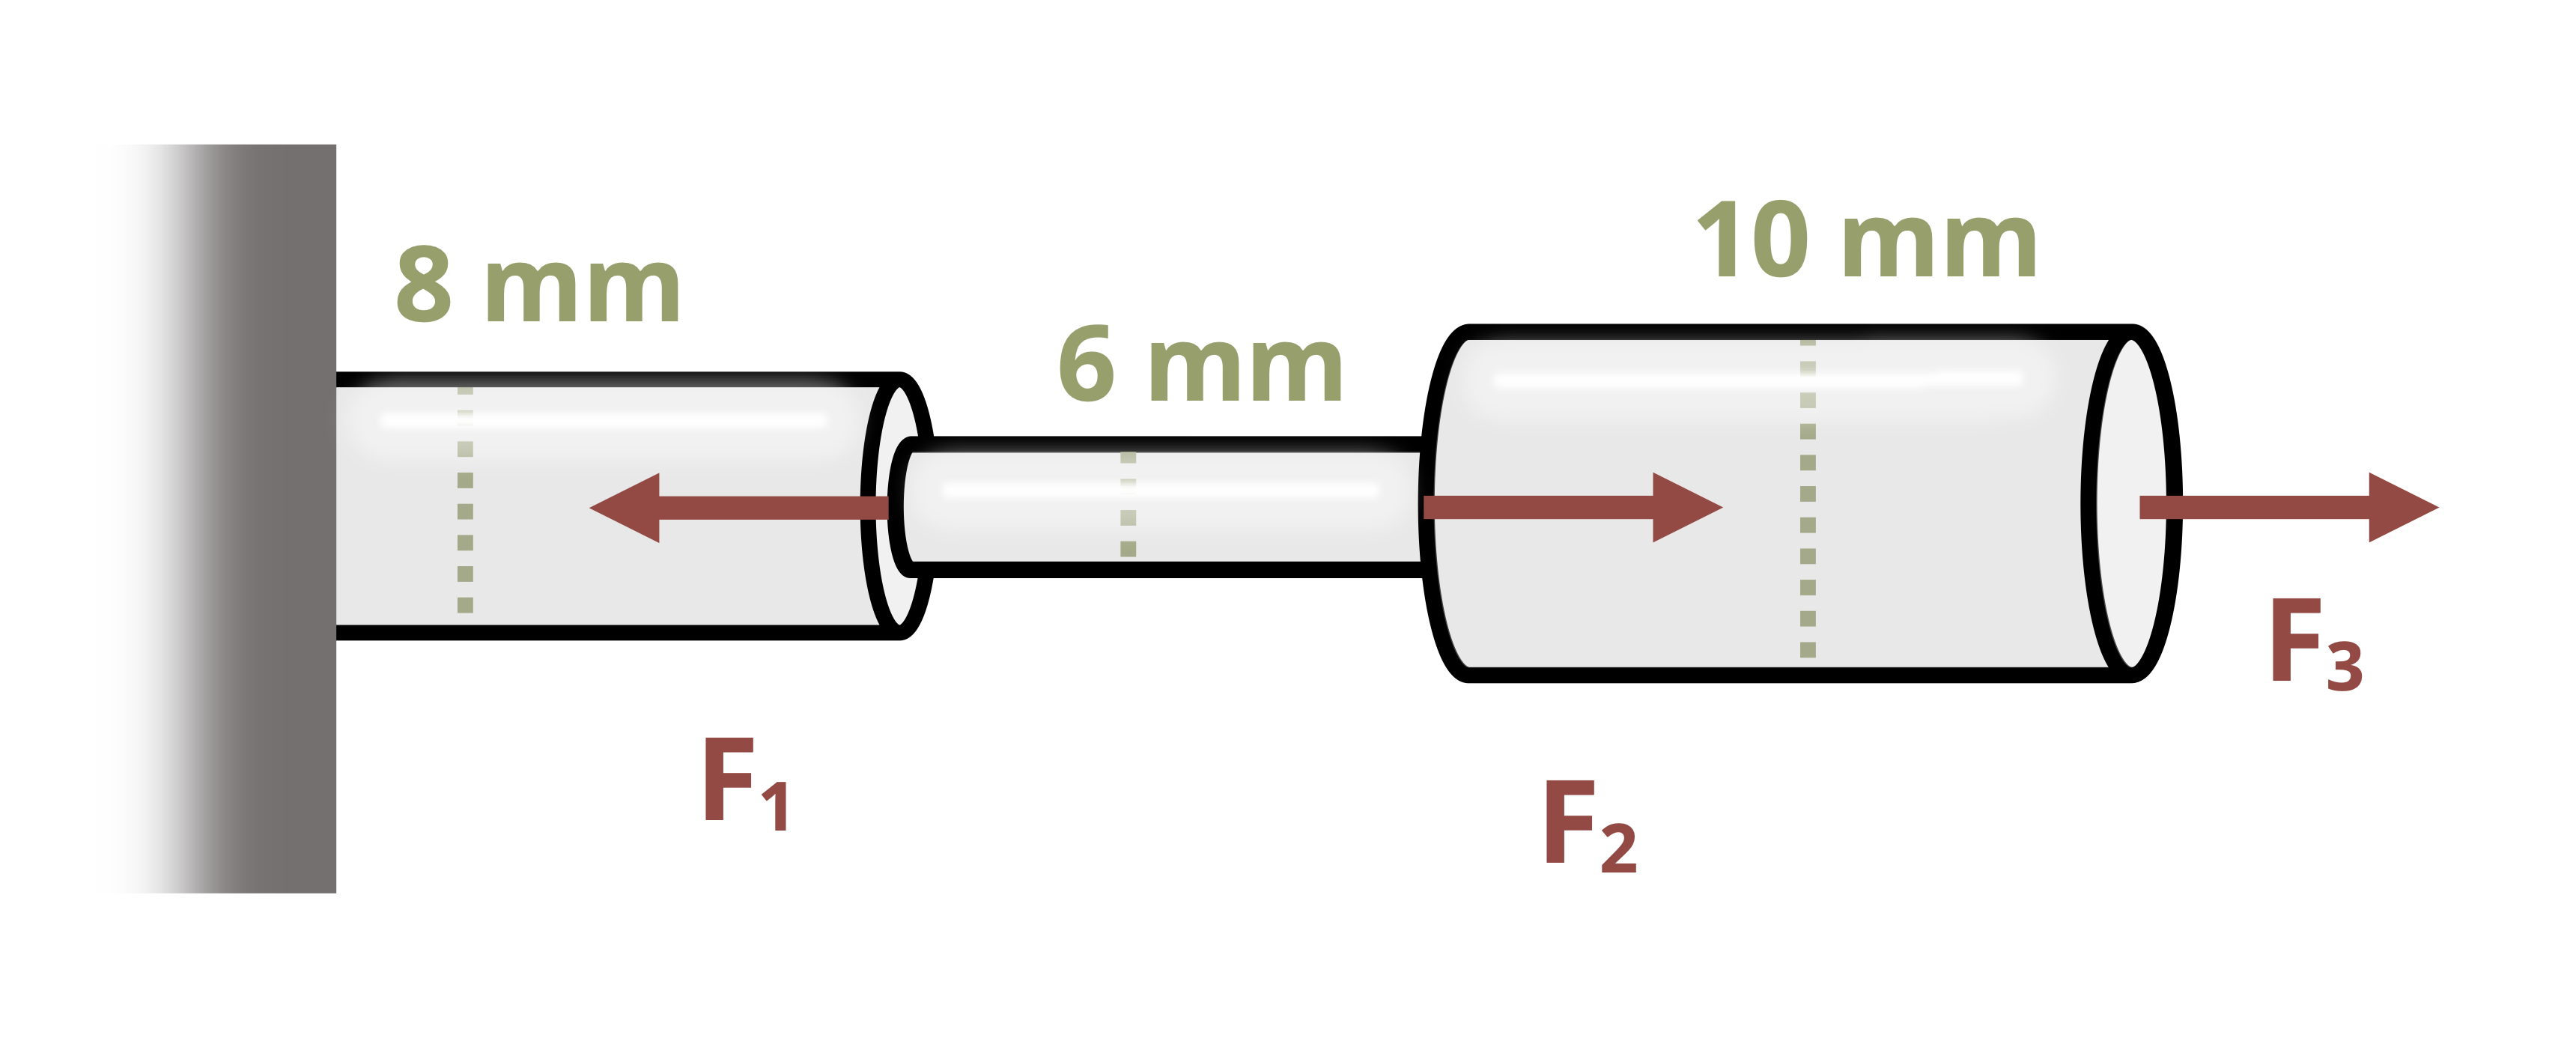
\includegraphics{images/138.png}

}

\caption{Figure 1: A series of solid circular bars are loaded with three
loads}

\end{figure}%

\chapter*{Problem 2.2}\label{problem-2.2-1}
\addcontentsline{toc}{chapter}{Problem 2.2}

\markboth{Problem 2.2}{Problem 2.2}

This is a static rendering of the problem.

\chapter*{Problem Statement}\label{problem-statement-1}
\addcontentsline{toc}{chapter}{Problem Statement}

\markboth{Problem Statement}{Problem Statement}

Two cylinders are stacked on top of one another and two forces are
applied at the top surface and at the joint between the cylinders as
shown. If L1 = 3 in., L2 = 4 in., FA = 500 lb, and FB = 200 lb, find the
total deflection in the stack of cylinders. Assume E = 30 x 106 psi for
both cylinders.

\section*{Problem Image}\label{problem-image-11}
\addcontentsline{toc}{section}{Problem Image}

\markright{Problem Image}

\begin{figure}[H]

{\centering 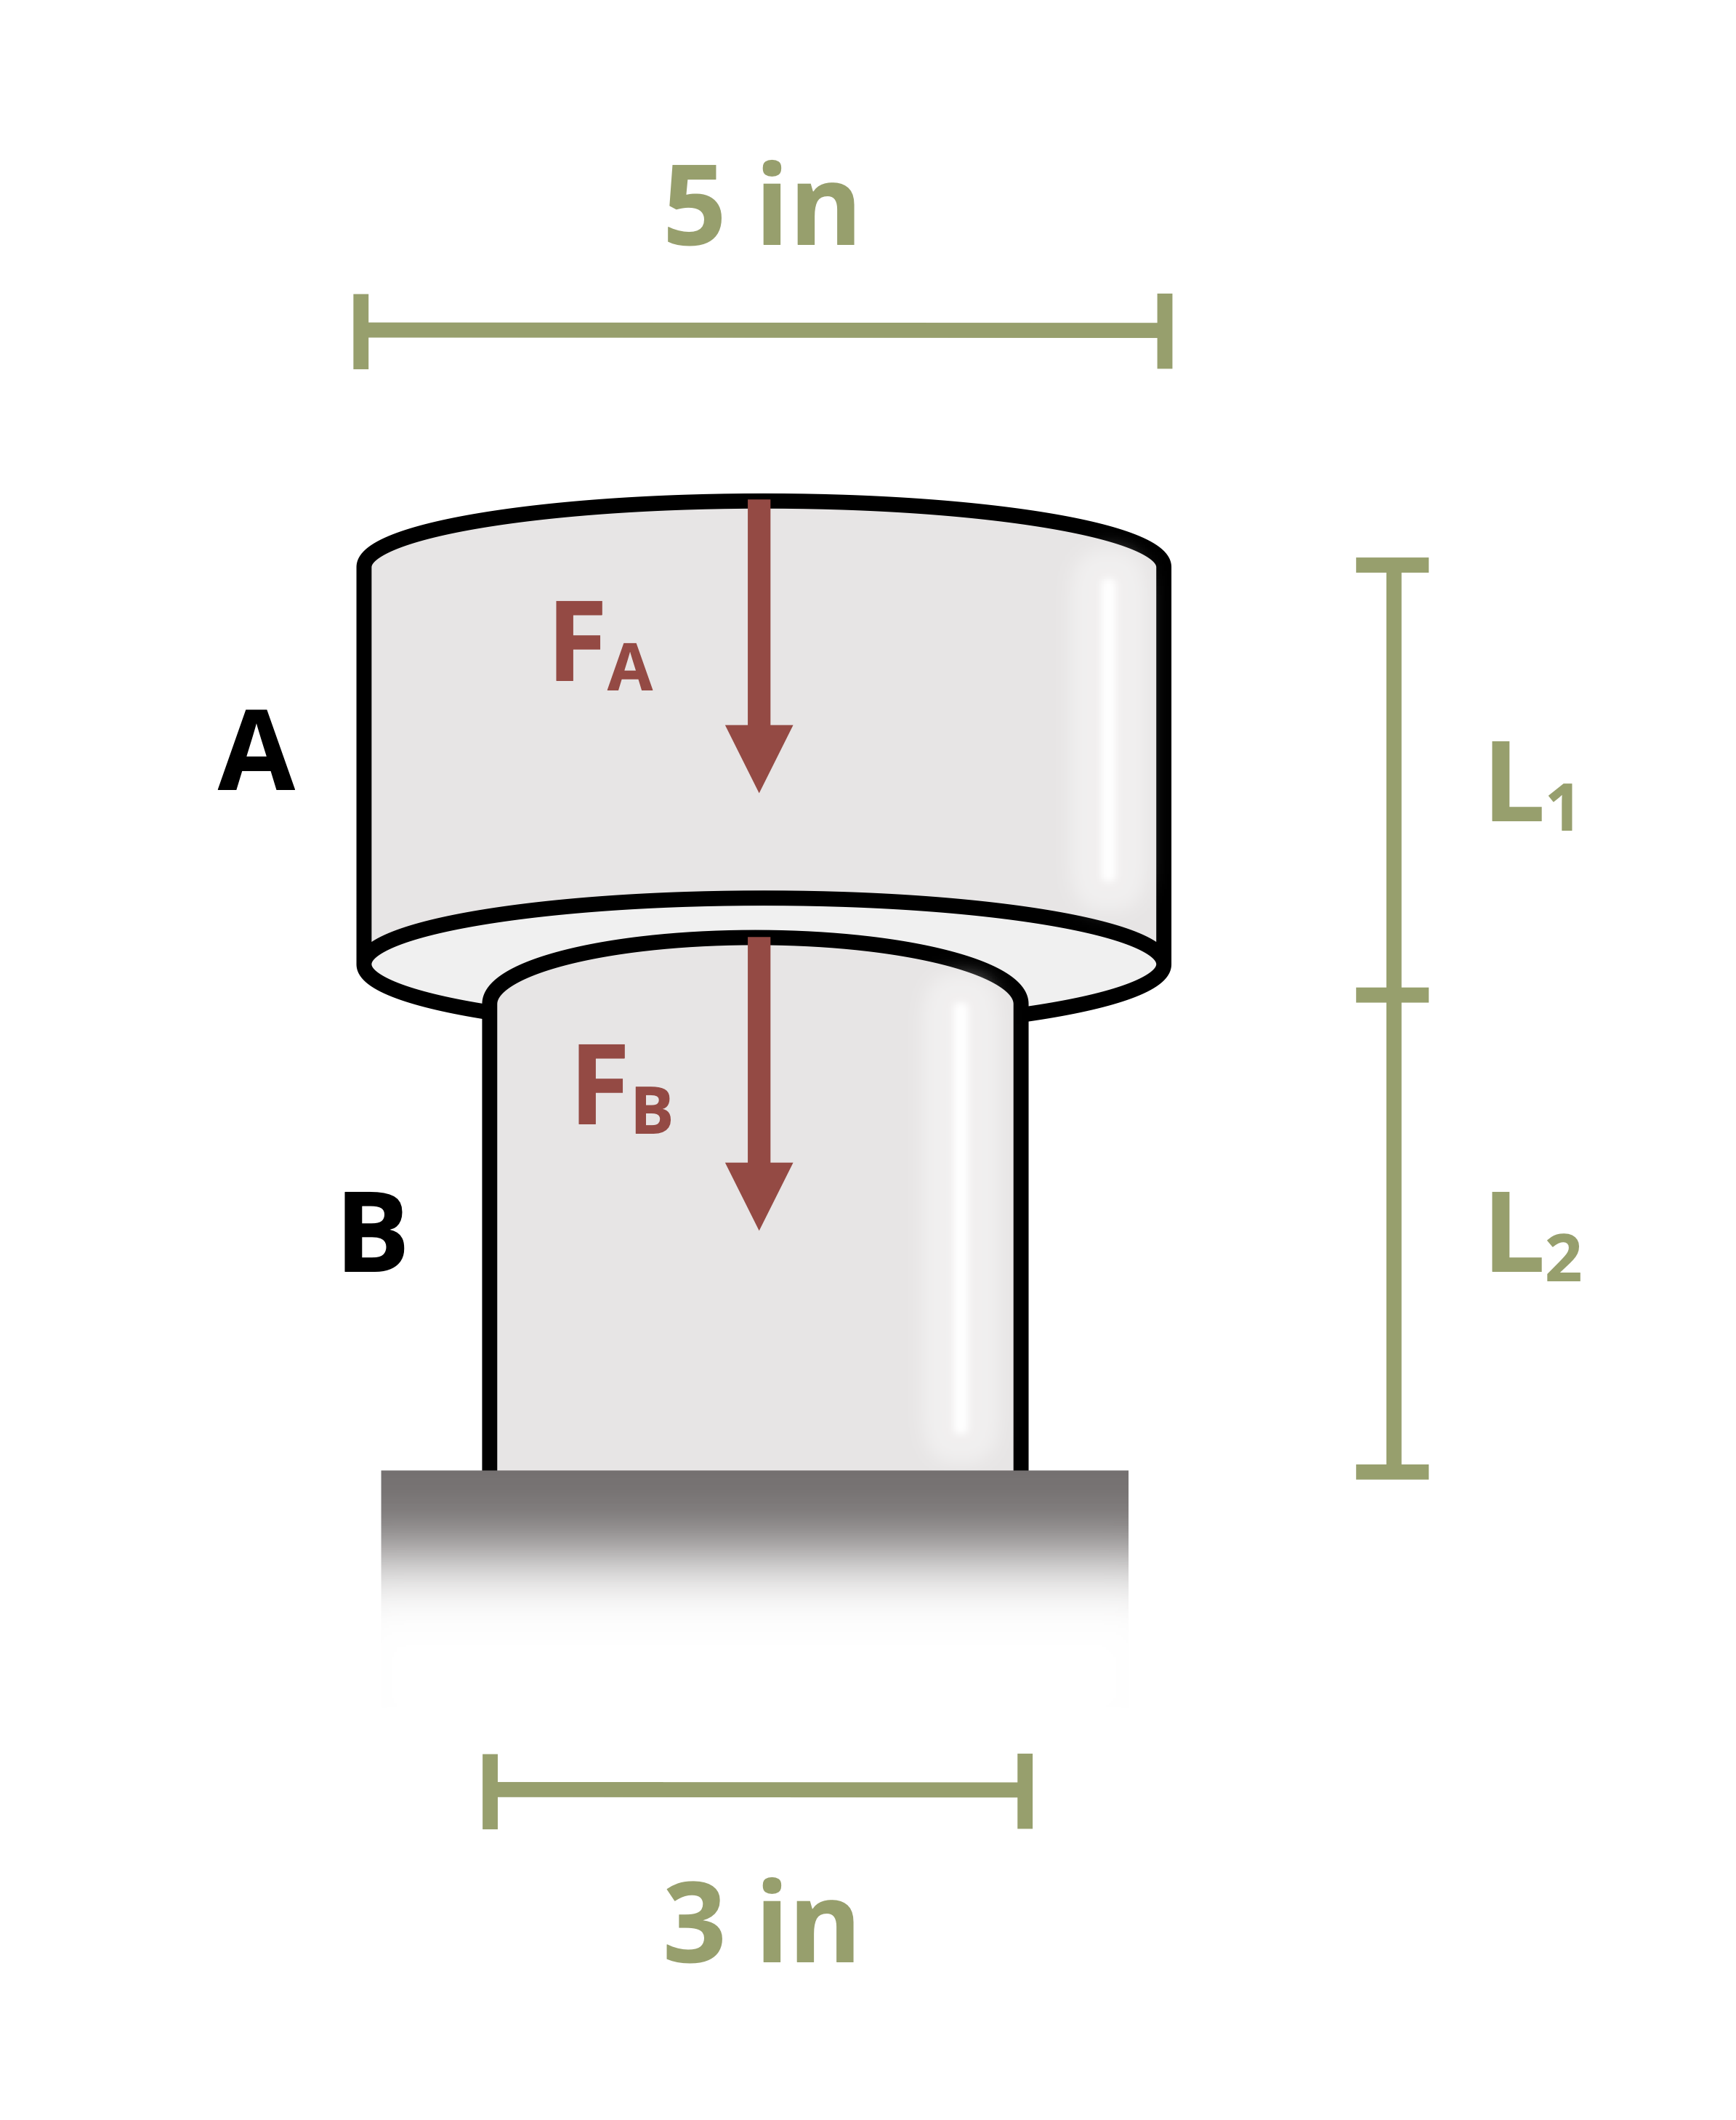
\includegraphics{images/139.png}

}

\caption{Figure 1: Two sylinders are stacked on top of each other.}

\end{figure}%

\chapter*{Problem 2.3}\label{problem-2.3-1}
\addcontentsline{toc}{chapter}{Problem 2.3}

\markboth{Problem 2.3}{Problem 2.3}

This is a static rendering of the problem.

\section*{Problem Statement}\label{problem-statement-2}
\addcontentsline{toc}{section}{Problem Statement}

\markright{Problem Statement}

A plastic cylindrical peg is constrained by a metal cap as shown. An
axial load of F = 40 lb is applied to the peg. If d1 = 0.5 in and d2 =
0.9 in, determine the normal stress in the peg. Assume the axial load is
evenly distributed across the peg and that the metal cap is fixed and
does not move.

\section*{Problem Image}\label{problem-image-12}
\addcontentsline{toc}{section}{Problem Image}

\markright{Problem Image}

\begin{figure}[H]

{\centering 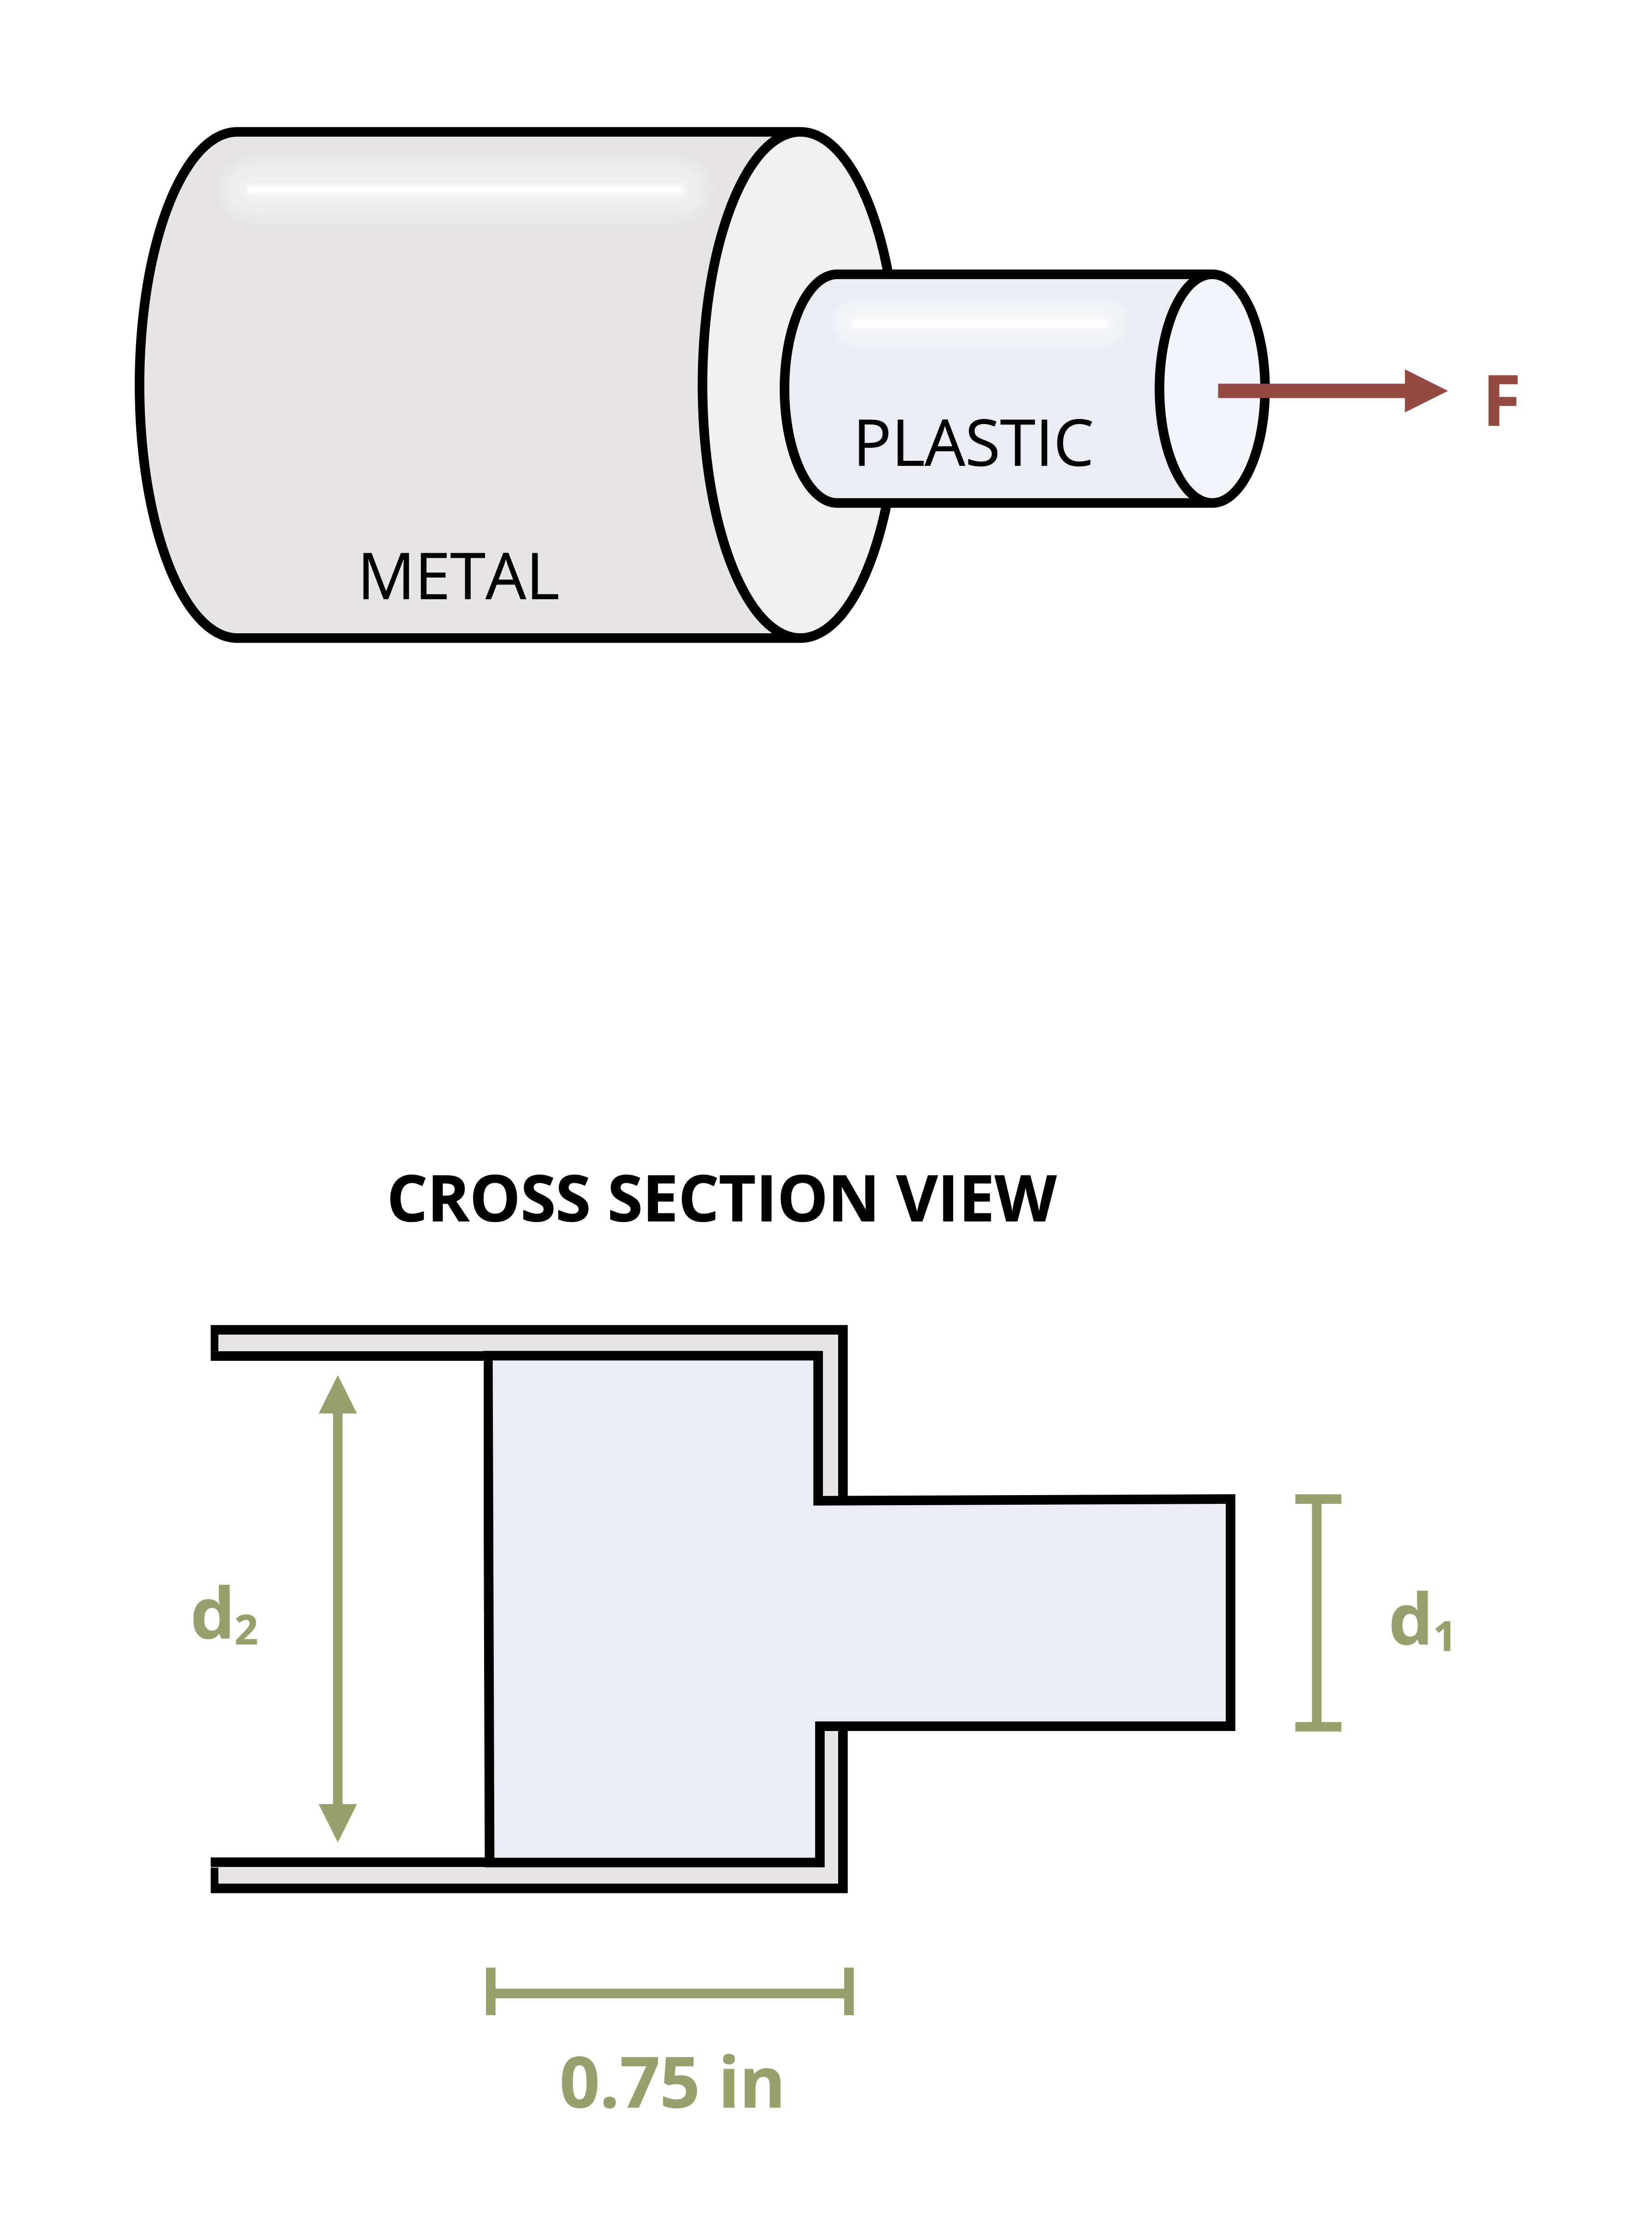
\includegraphics{images/144.png}

}

\caption{Figure 1: A plastic cylindrical peg is constrained by a metal
cap}

\end{figure}%

\chapter*{Problem 2.4}\label{problem-2.4-1}
\addcontentsline{toc}{chapter}{Problem 2.4}

\markboth{Problem 2.4}{Problem 2.4}

This is a static rendering of the problem.

\section*{Problem Statement}\label{problem-statement-3}
\addcontentsline{toc}{section}{Problem Statement}

\markright{Problem Statement}

A crate weighing 45 kN is suspended by a set of cables. The diameter of
each cable is 5 mm. What is the maximum stress in any cable, exluding
the cable attached to the crate.

\section*{Problem Image}\label{problem-image-13}
\addcontentsline{toc}{section}{Problem Image}

\markright{Problem Image}

\begin{figure}[H]

{\centering 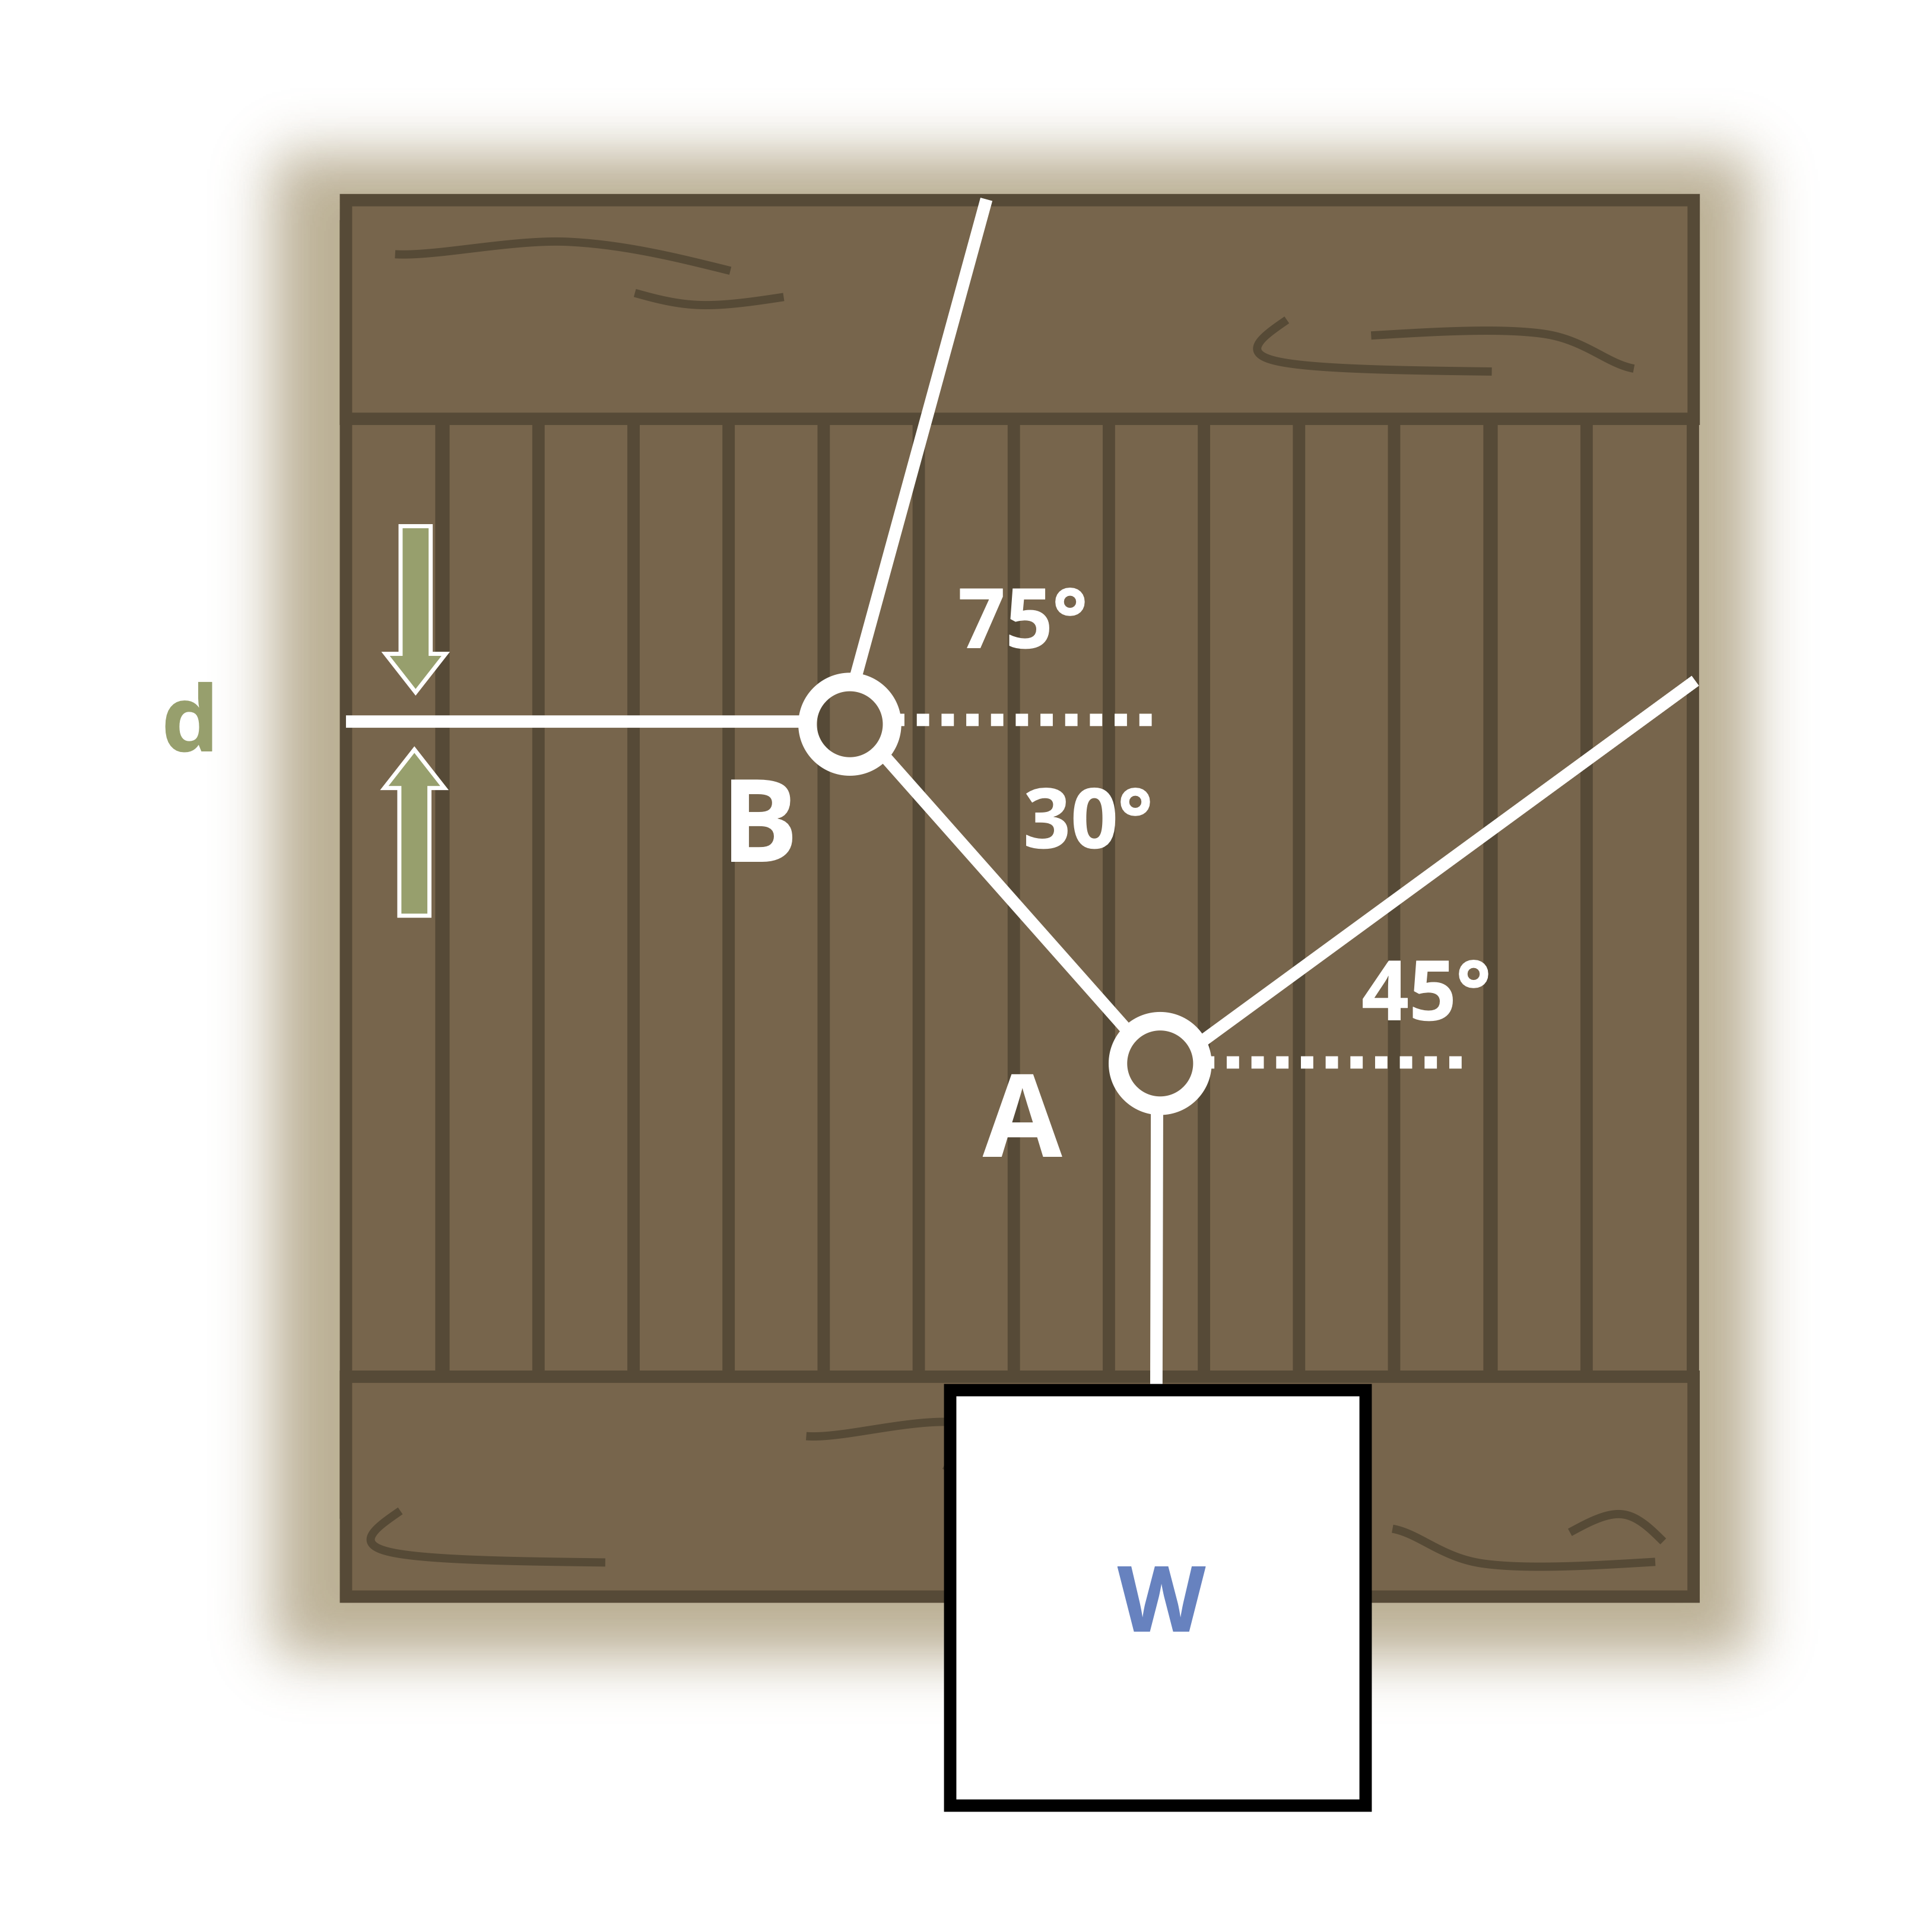
\includegraphics{images/146.png}

}

\caption{Figure 1: A crate is suspended by a set of cables}

\end{figure}%

\chapter*{Problem 2.47}\label{problem-2.47-1}
\addcontentsline{toc}{chapter}{Problem 2.47}

\markboth{Problem 2.47}{Problem 2.47}

This is a static rendering of the problem.

\section*{Problem Statement}\label{problem-statement-4}
\addcontentsline{toc}{section}{Problem Statement}

\markright{Problem Statement}

Two slanted brackets are glued together as shown. If F = 500 lb, L = 4
in., and Θ = 20 °, determine the shear stress parallel to the inclined
plane. Assume loads are inline and there is no rotation.

\section*{Problem Image}\label{problem-image-14}
\addcontentsline{toc}{section}{Problem Image}

\markright{Problem Image}

\begin{figure}[H]

{\centering 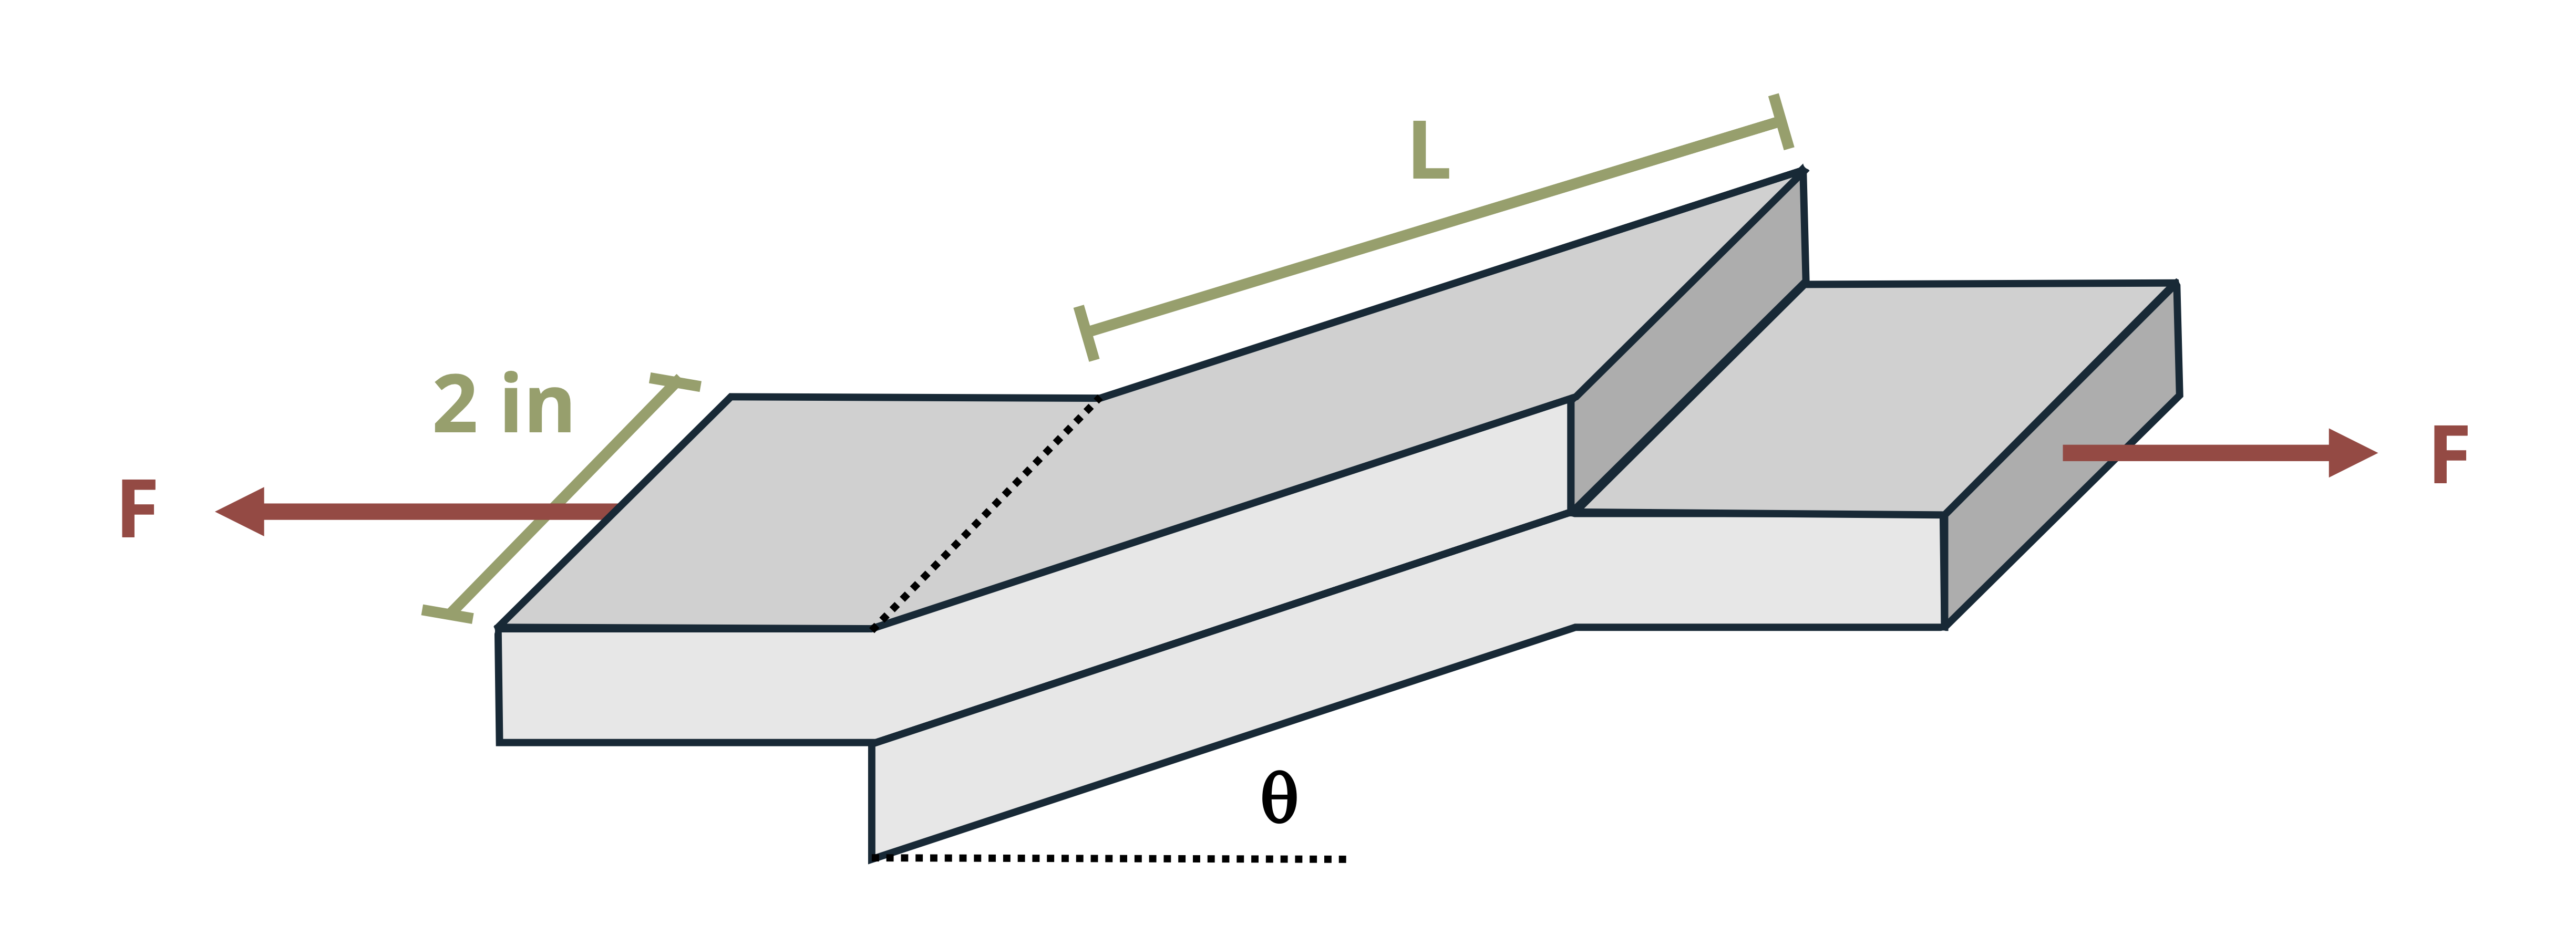
\includegraphics{images/153.png}

}

\caption{Figure 1: Two slanted brackets are glued together}

\end{figure}%

\chapter*{Problem 2.48}\label{problem-2.48-1}
\addcontentsline{toc}{chapter}{Problem 2.48}

\markboth{Problem 2.48}{Problem 2.48}

This is a static rendering of the problem.

\section*{Problem Statement}\label{problem-statement-5}
\addcontentsline{toc}{section}{Problem Statement}

\markright{Problem Statement}

A 2 inch thick board is cut and then glued back together along a line
that is Θ = 15° off the vertical as shown. If height h = 10 in. and F =
3500 lb, determine the normal stress along the cut line.

\section*{Problem Image}\label{problem-image-15}
\addcontentsline{toc}{section}{Problem Image}

\markright{Problem Image}

\begin{figure}[H]

{\centering 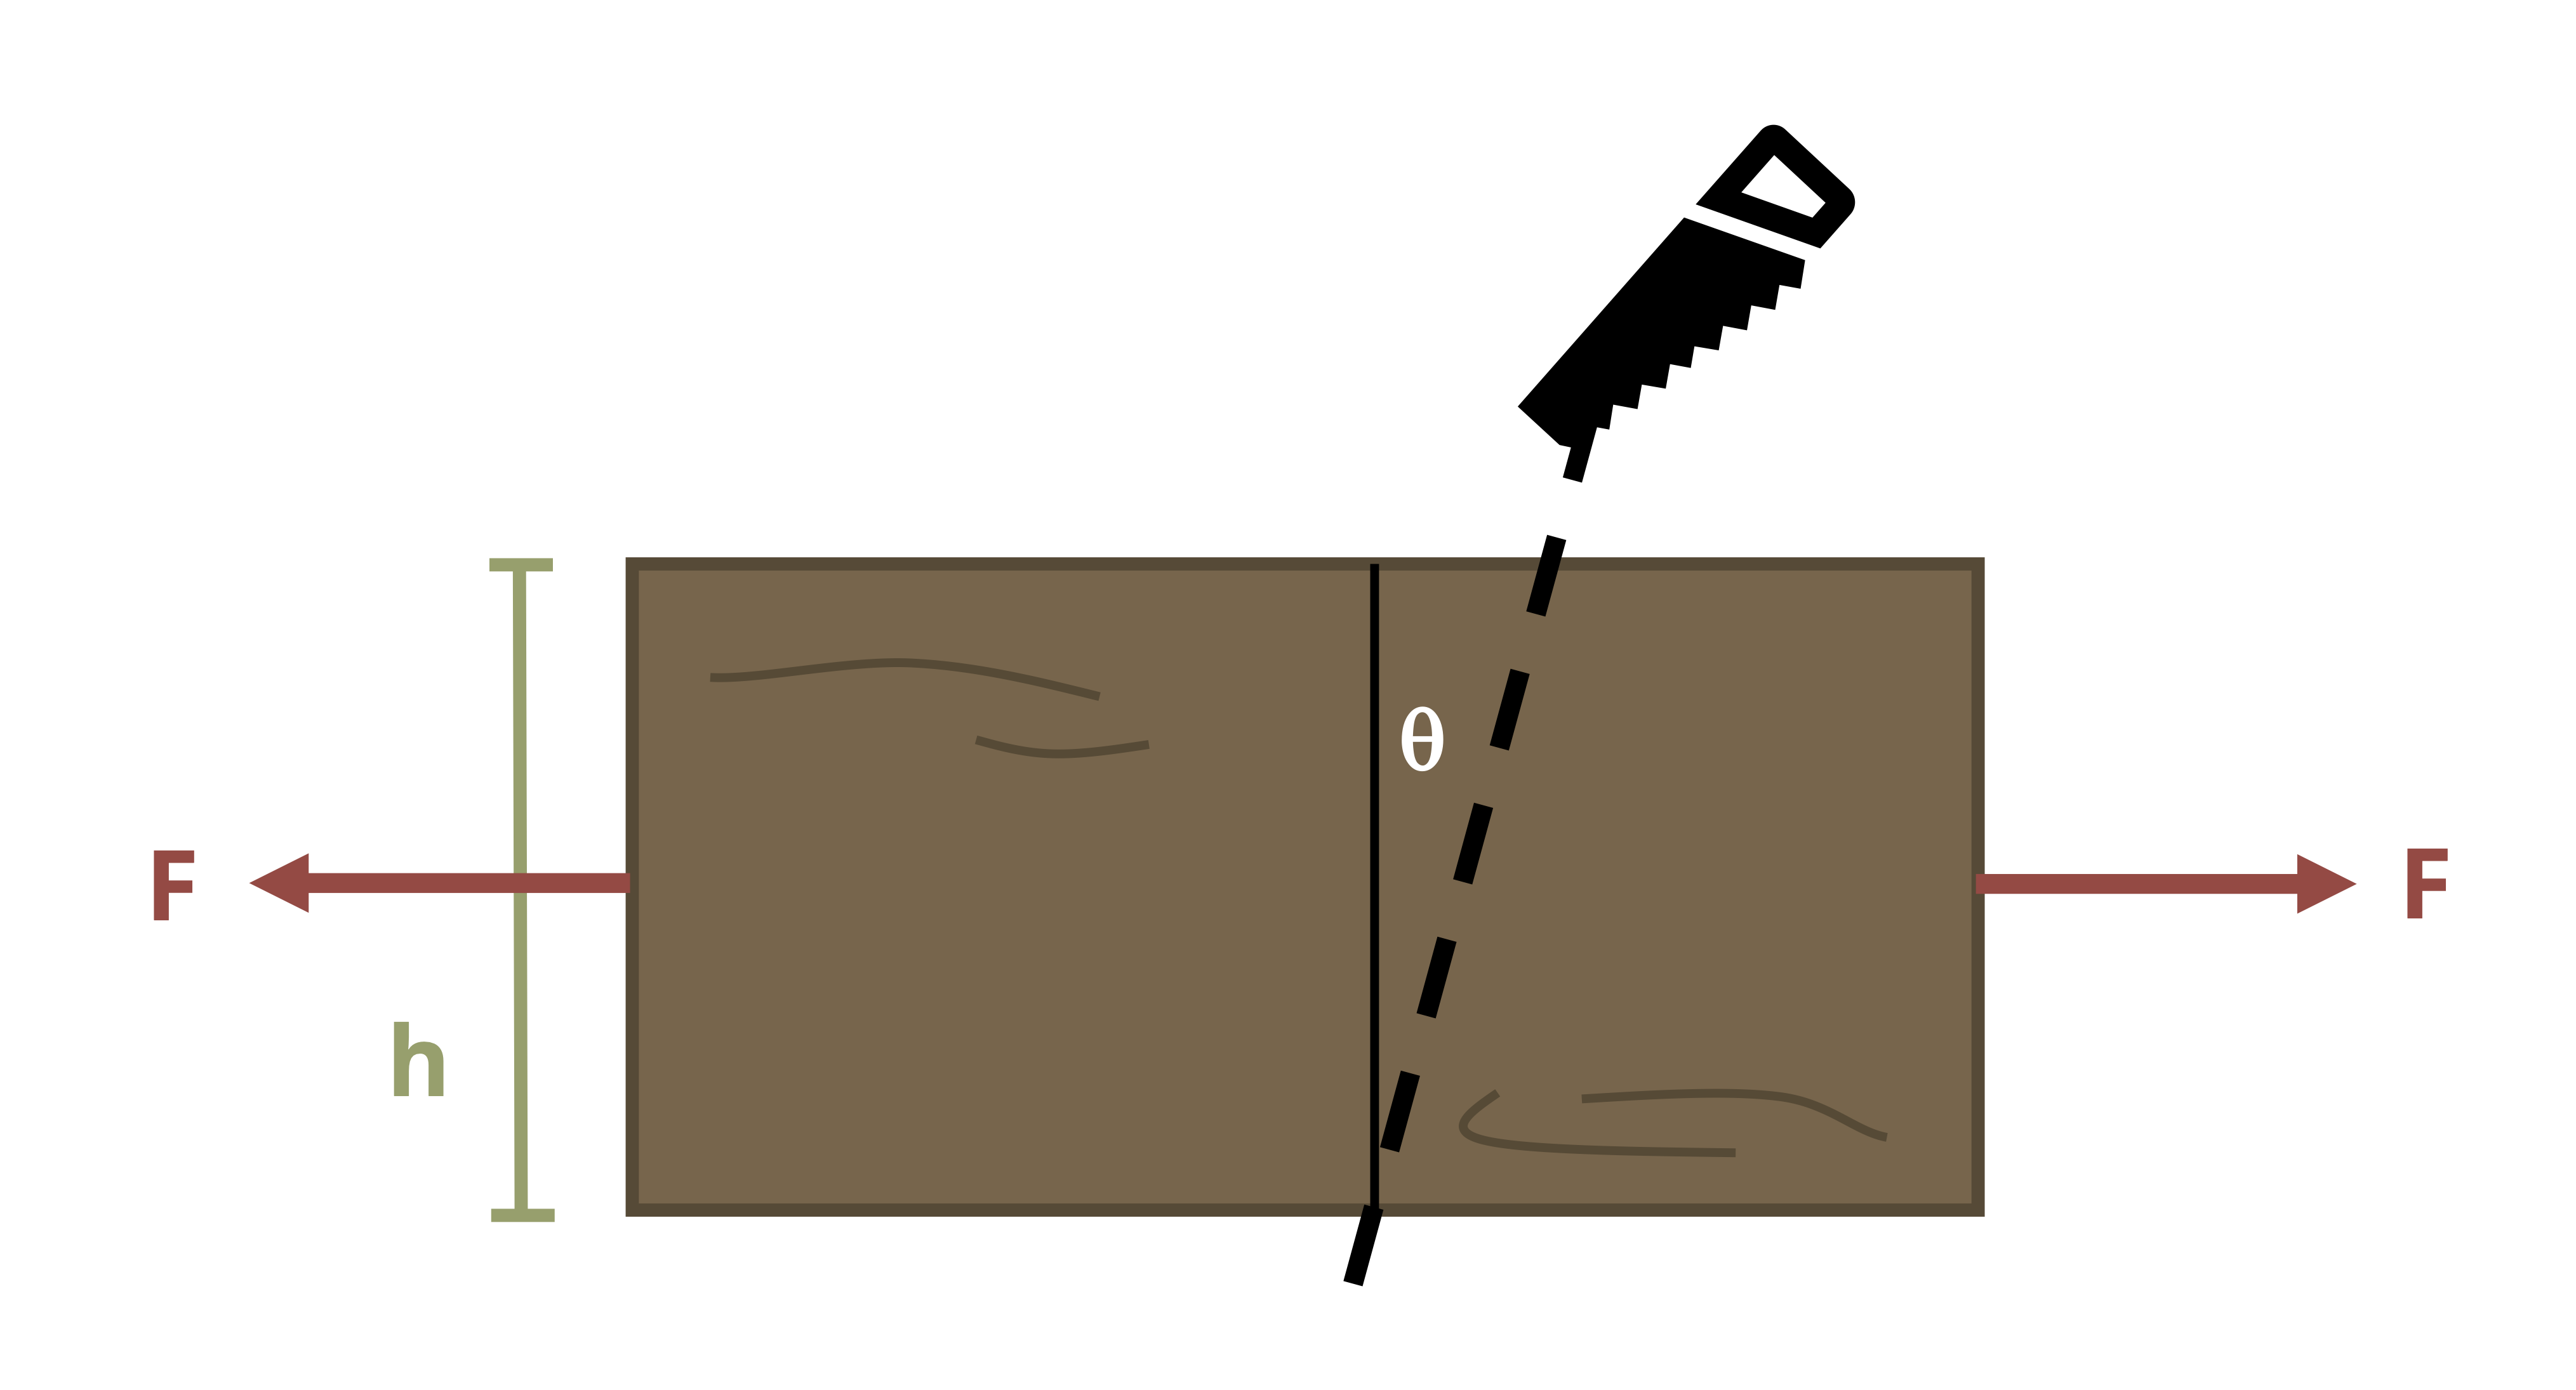
\includegraphics{images/156.png}

}

\caption{Figure 1: A 2 inch thick board is cut and then glued back
together along a line}

\end{figure}%

\chapter*{Problem 4.37}\label{problem-4.37}
\addcontentsline{toc}{chapter}{Problem 4.37}

\markboth{Problem 4.37}{Problem 4.37}

This is a static rendering.

\section*{Problem Statement}\label{problem-statement-6}
\addcontentsline{toc}{section}{Problem Statement}

\markright{Problem Statement}

A small truss is constructed with solid square wood members and
subjected to a load of F = 30 kN. Determine the minimum dimension, a, of
the member so that the truss will have a factor of safety of 2. All
members have the same cross-section. The wood has a failure stress of
σfail = 50 MPa.

\section*{Problem Image}\label{problem-image-16}
\addcontentsline{toc}{section}{Problem Image}

\markright{Problem Image}

\begin{figure}[H]

{\centering 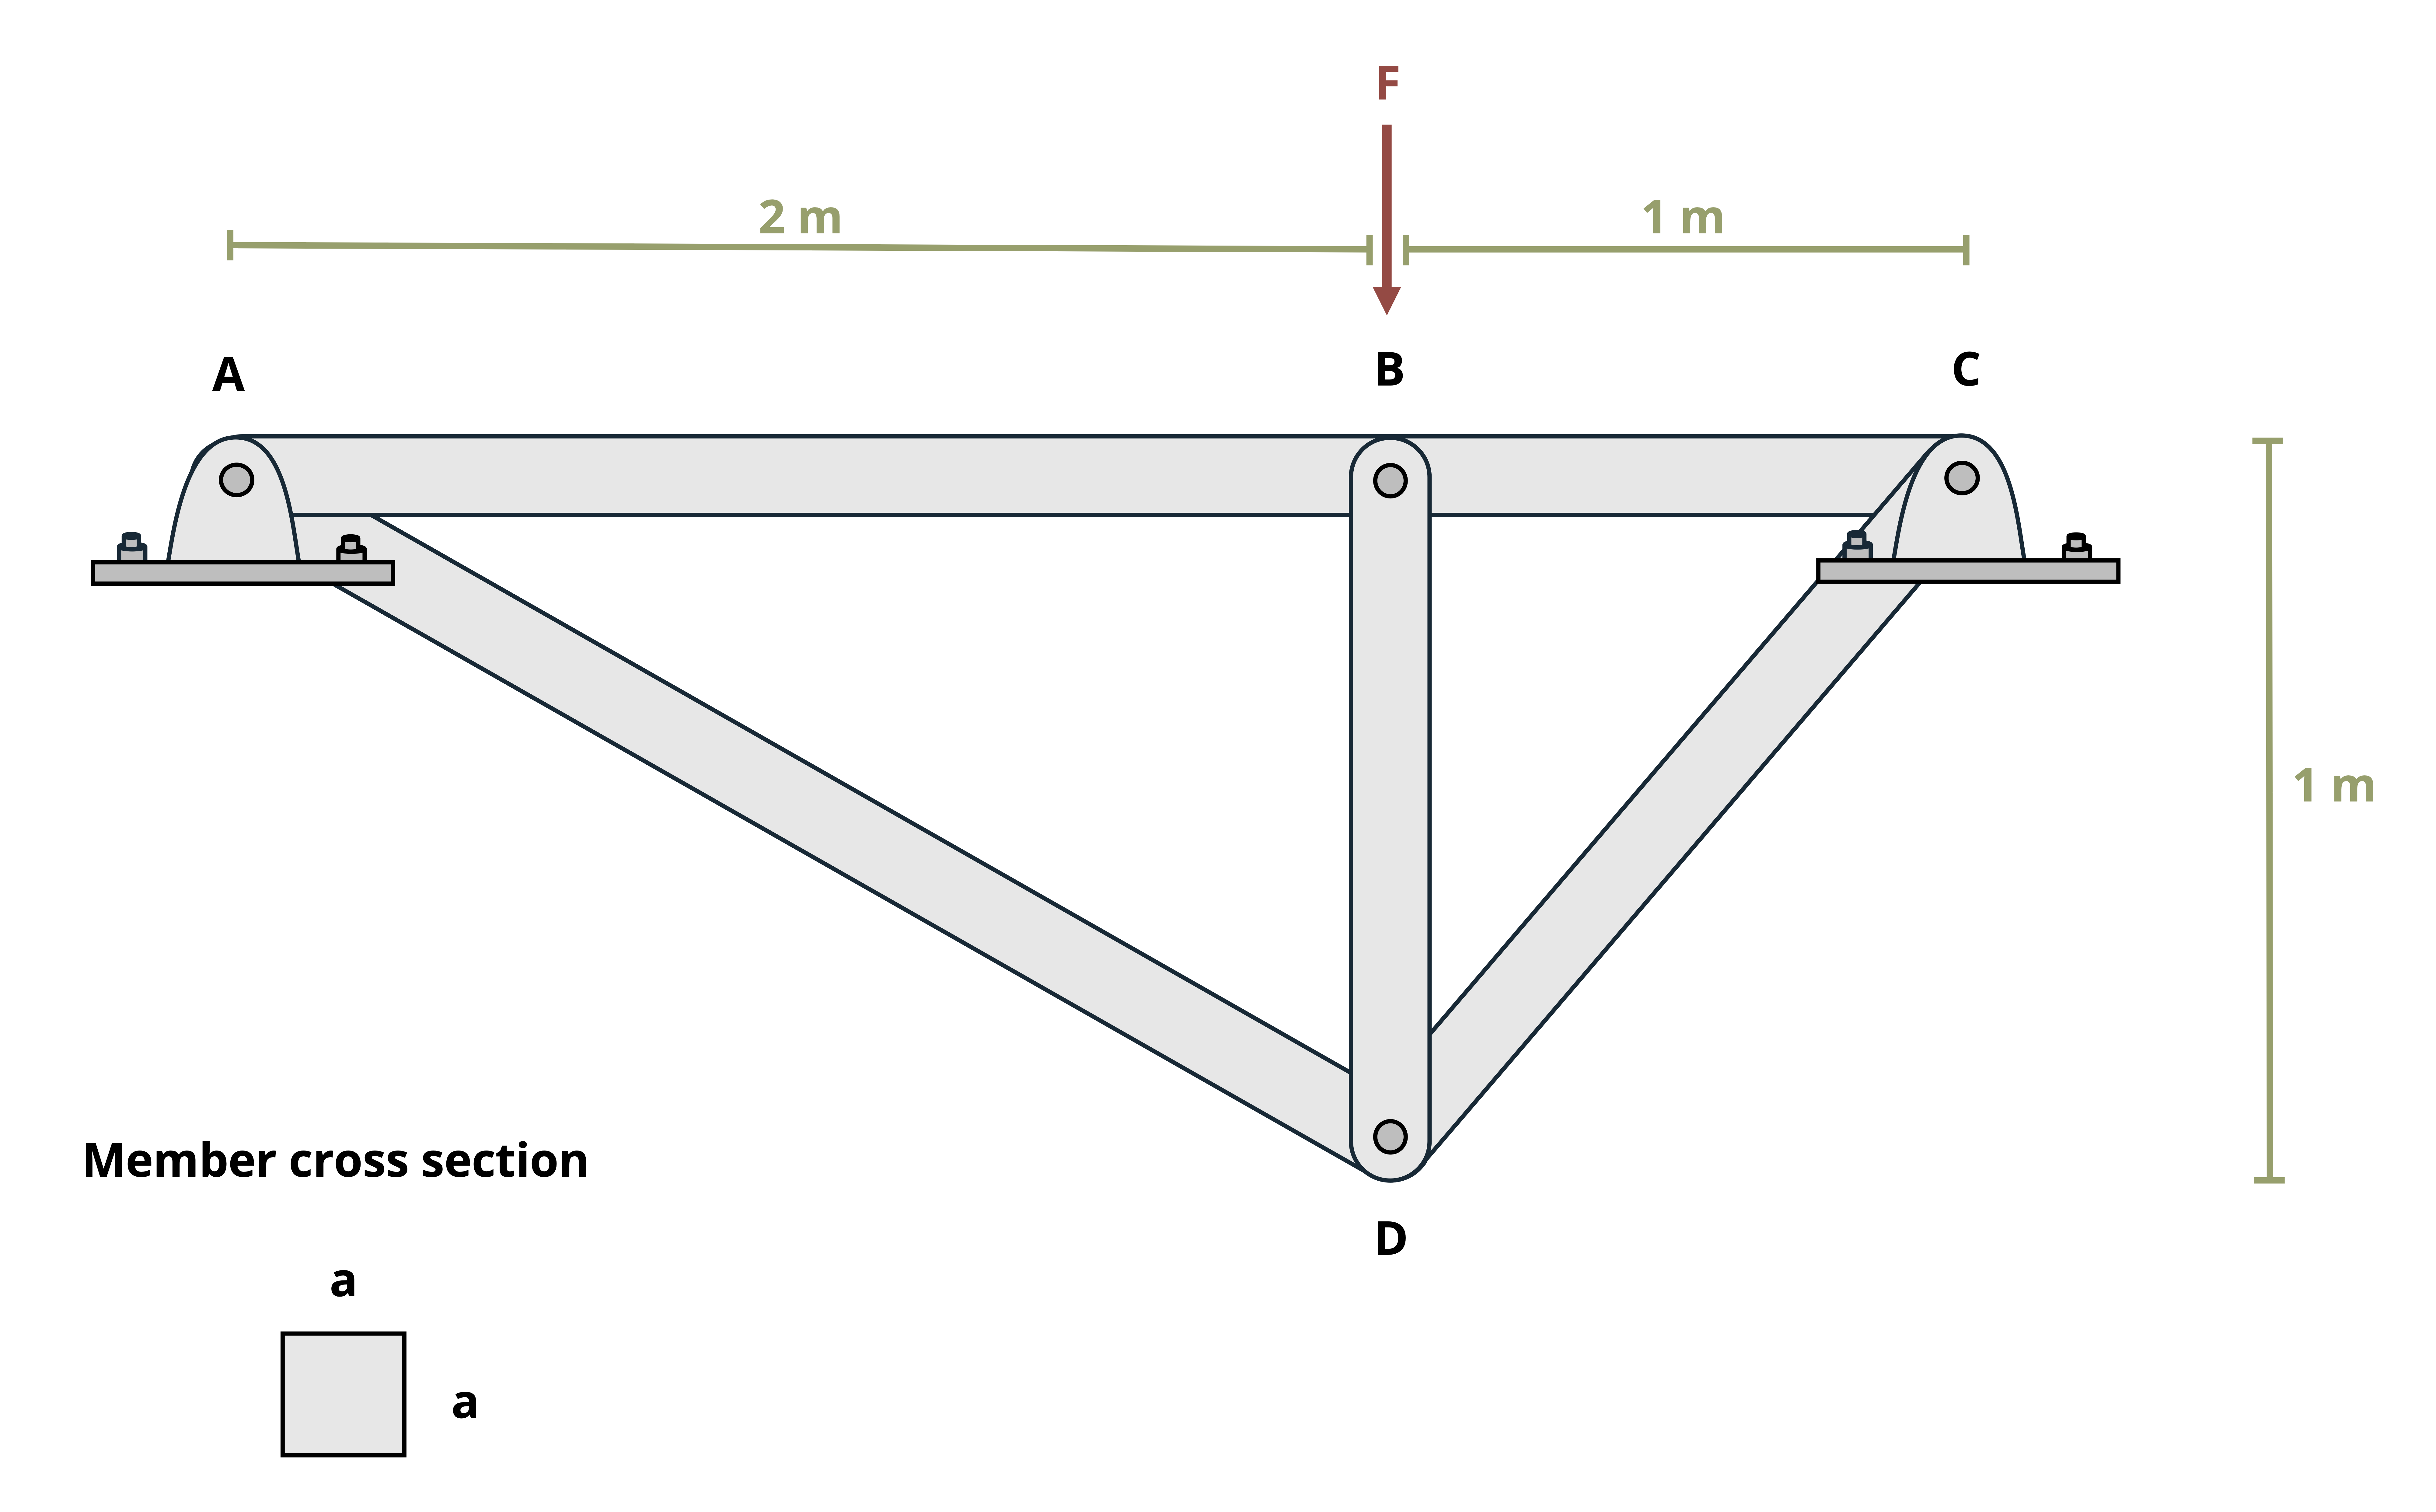
\includegraphics{images/157.png}

}

\caption{Figure 1: A small truss is constructed with solid square wood
members}

\end{figure}%

\chapter*{Problem 2.21}\label{problem-2.21-1}
\addcontentsline{toc}{chapter}{Problem 2.21}

\markboth{Problem 2.21}{Problem 2.21}

This is a static rendering of the problem.

\section*{Problem Statement}\label{problem-statement-7}
\addcontentsline{toc}{section}{Problem Statement}

\markright{Problem Statement}

A double lap joint is glued together using glue with a shear stress
failure strength of 8000 psi. If dimensions L = 6 in. and t = 8 in.,
what is the maximum load P that the joint can withstand? Assume the load
is evenly distributed across the joint on both sides.

\section*{Problem Image}\label{problem-image-17}
\addcontentsline{toc}{section}{Problem Image}

\markright{Problem Image}

\begin{figure}[H]

{\centering 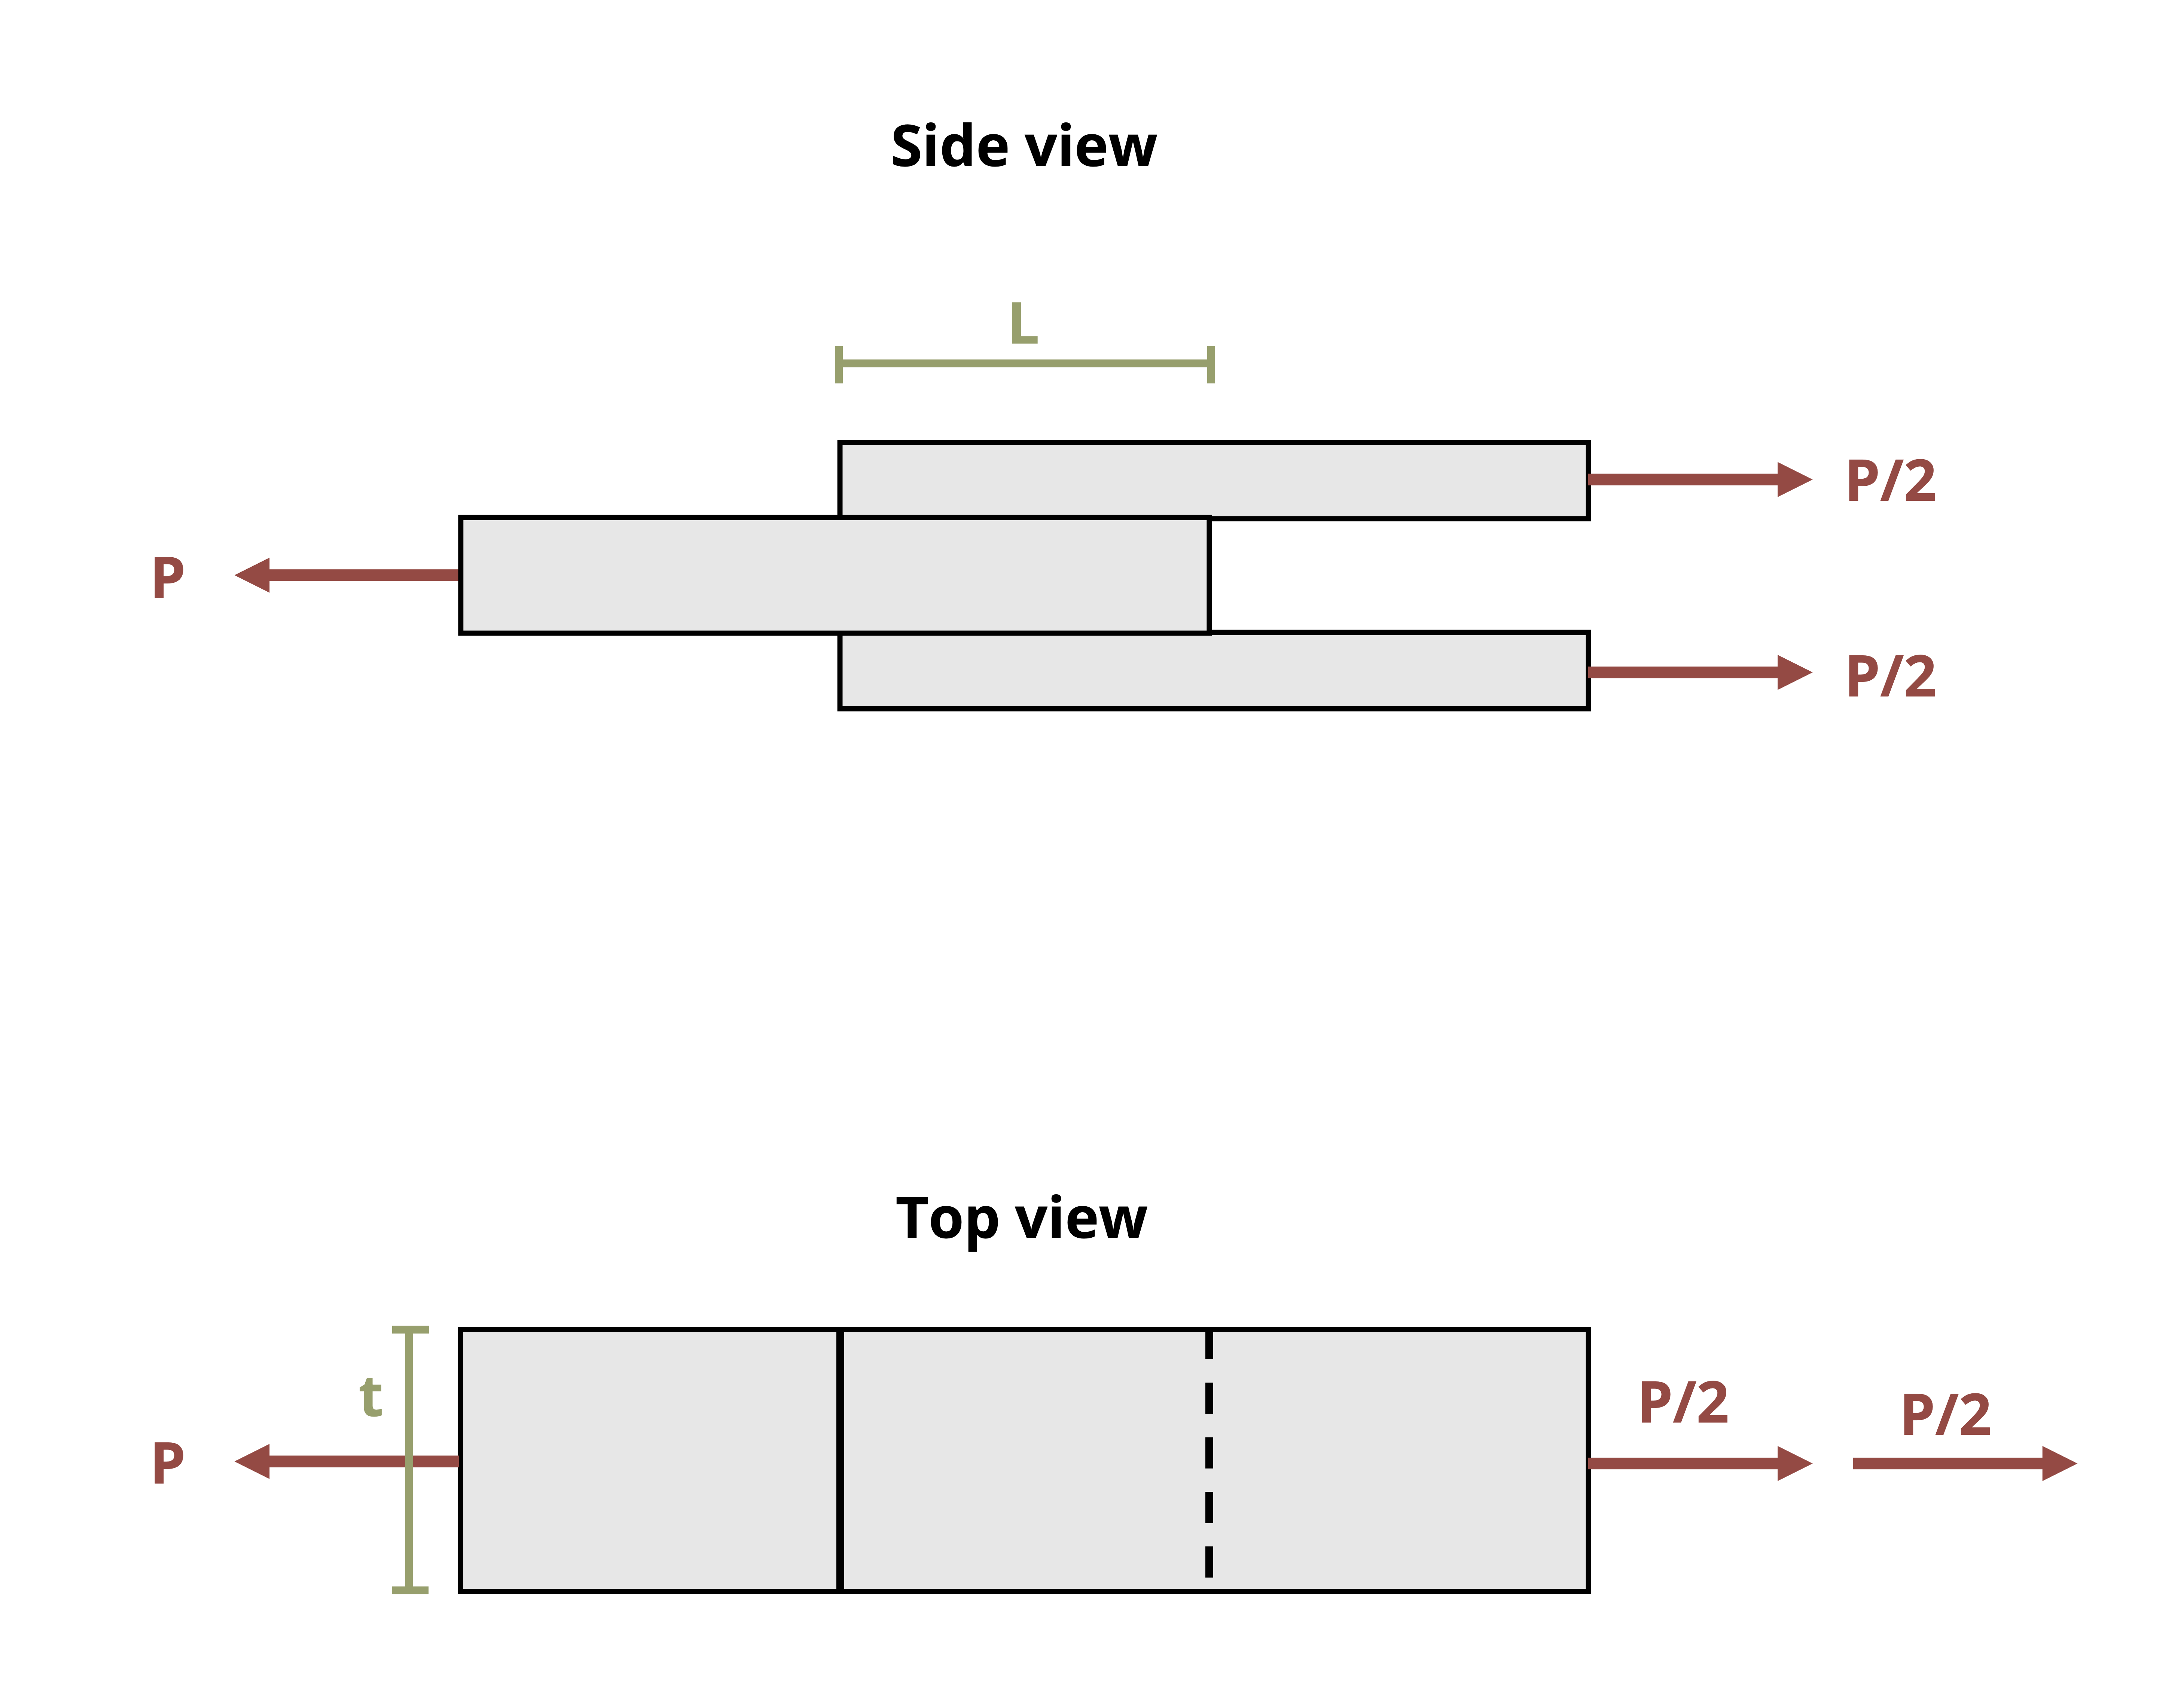
\includegraphics{images/164.png}

}

\caption{Figure 1: A double lap joint is glued together}

\end{figure}%

\chapter*{Problem 2.22}\label{problem-2.22-1}
\addcontentsline{toc}{chapter}{Problem 2.22}

\markboth{Problem 2.22}{Problem 2.22}

This is a static rendering of the problem.

\section*{Problem Statement}\label{problem-statement-8}
\addcontentsline{toc}{section}{Problem Statement}

\markright{Problem Statement}

A bracket is attached to a wall with two circular rivets of diameter d =
20 mm. A load F = 50 kN is applied in the center of the bracket.
Assuming the load is split evenly between the two rivits, determine the
shear stress in each rivet.

\section*{Problem Image}\label{problem-image-18}
\addcontentsline{toc}{section}{Problem Image}

\markright{Problem Image}

\begin{figure}[H]

{\centering 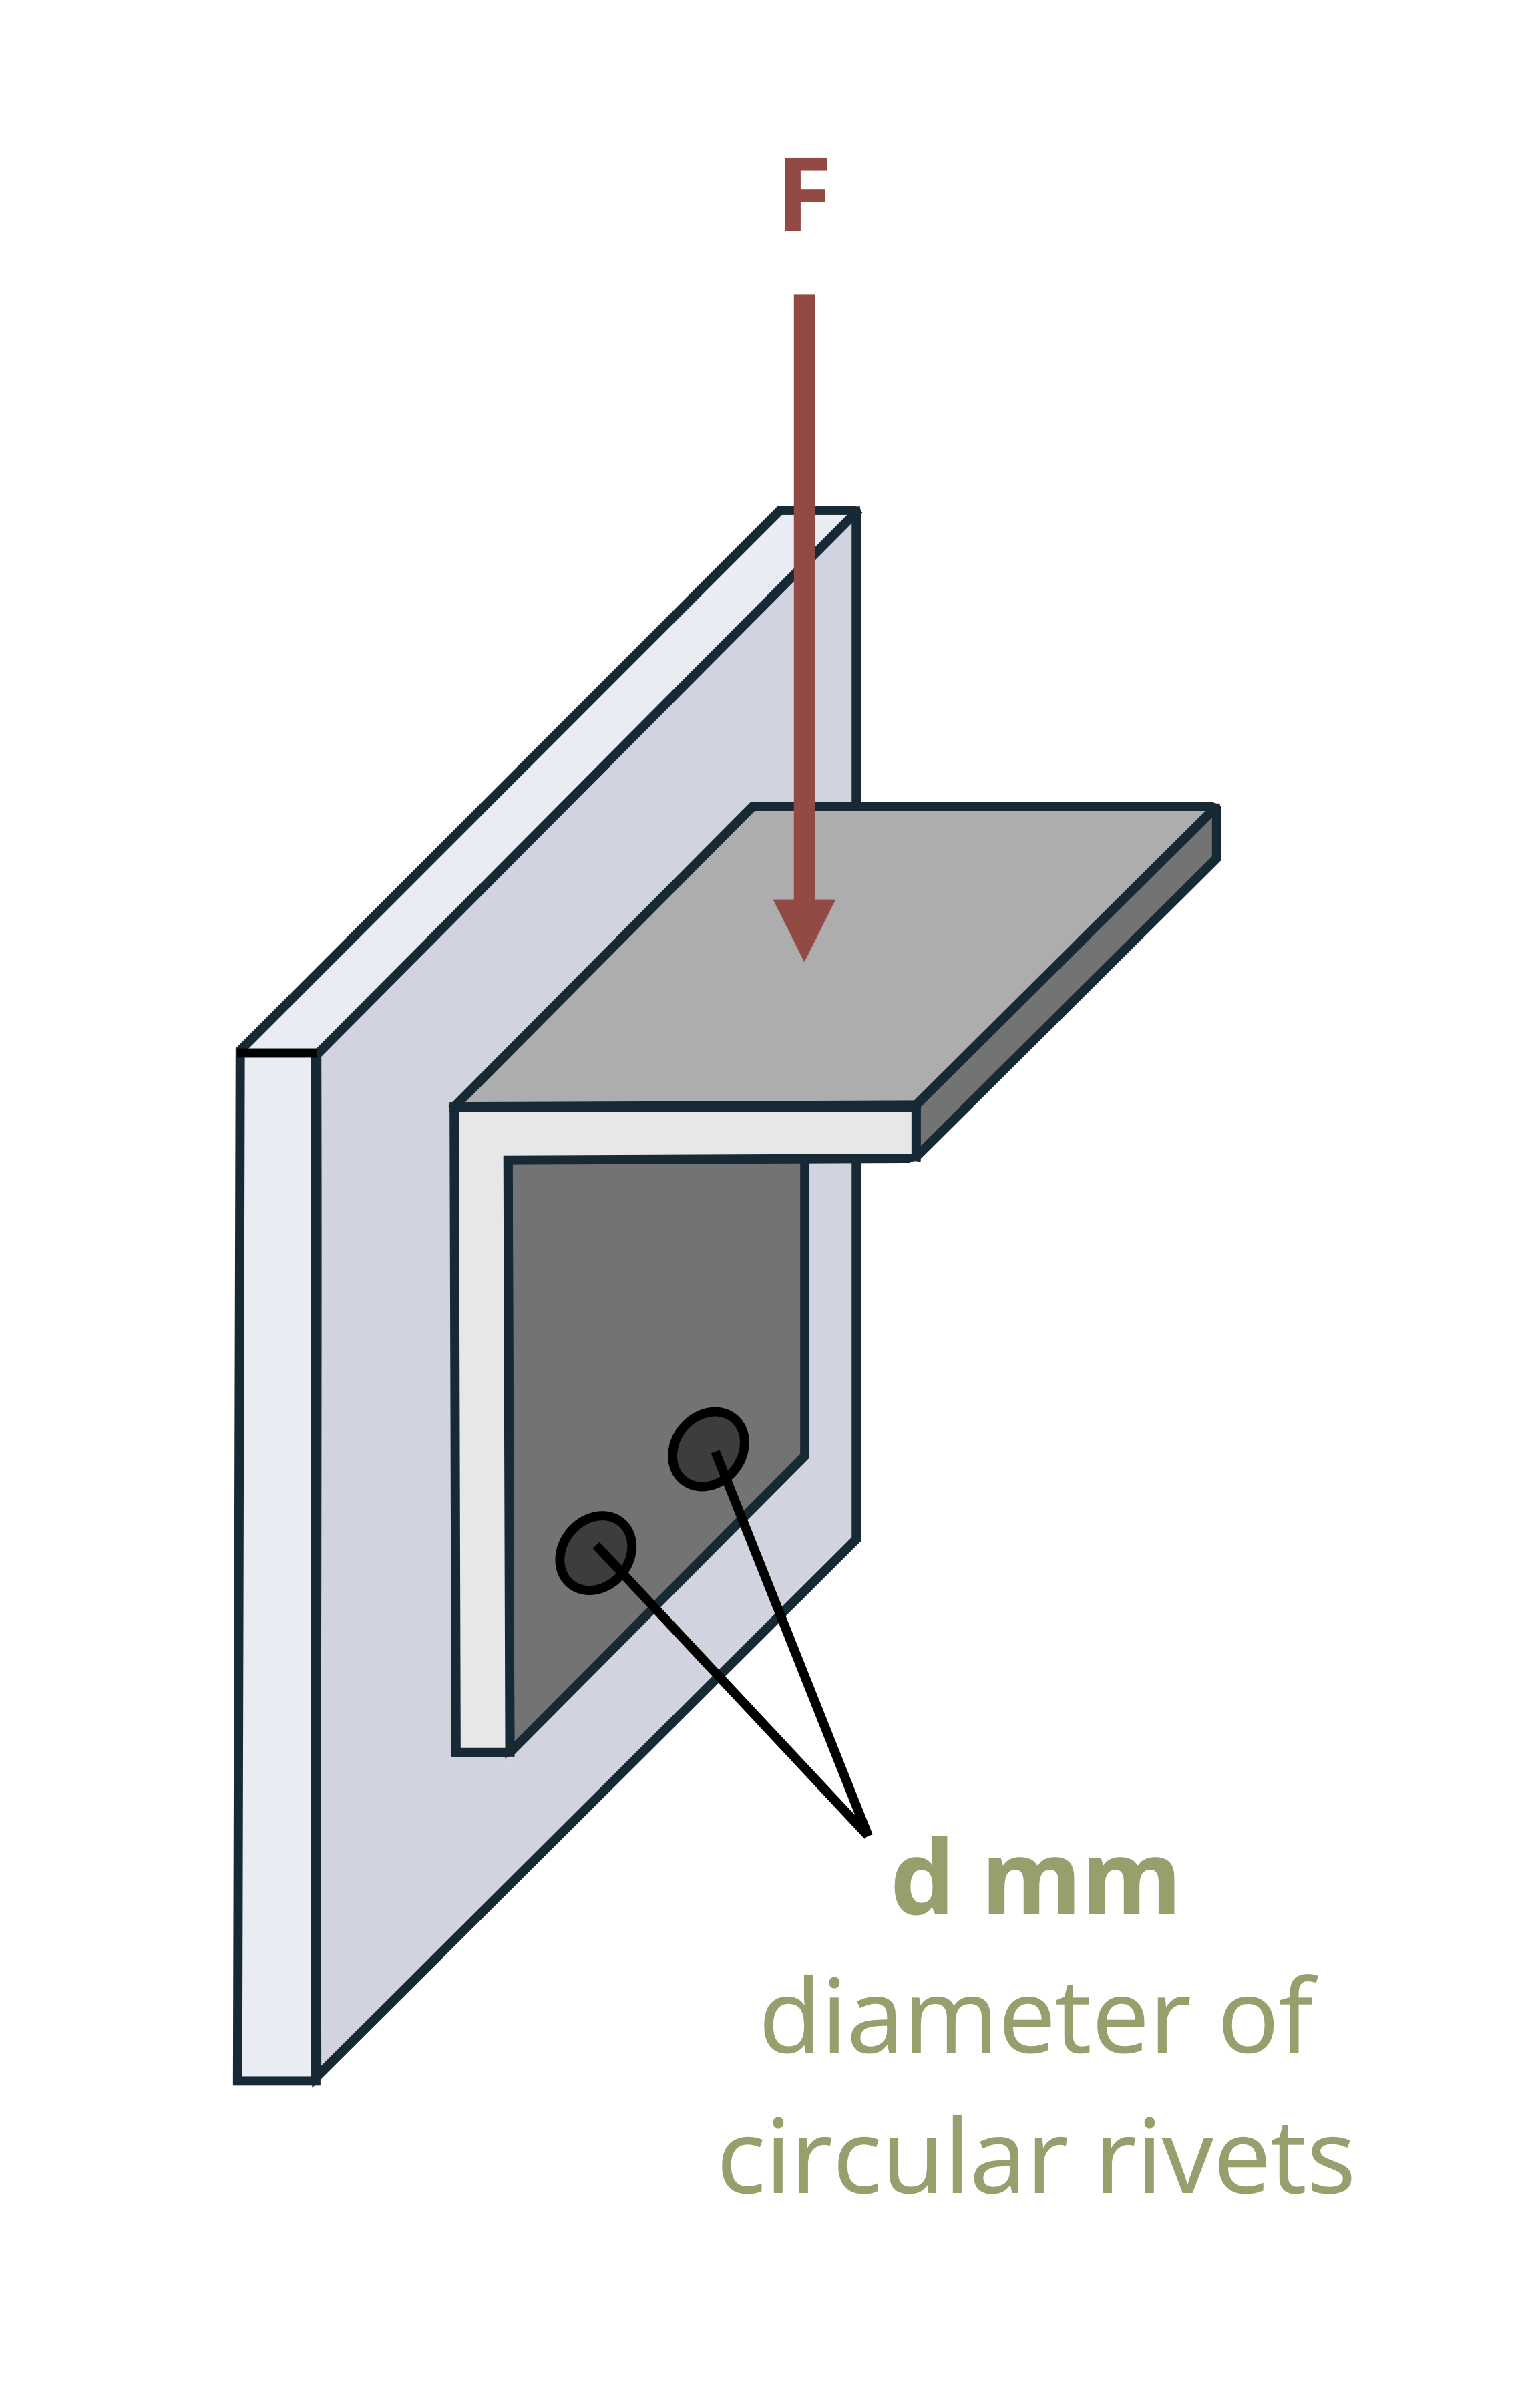
\includegraphics{images/165.png}

}

\caption{Figure 1: A bracket is attached to a wall with two circular
rivets}

\end{figure}%

\chapter*{Problem 2.38}\label{problem-2.38-1}
\addcontentsline{toc}{chapter}{Problem 2.38}

\markboth{Problem 2.38}{Problem 2.38}

This is a static rendering of the problem.

\section*{Problem Statement}\label{problem-statement-9}
\addcontentsline{toc}{section}{Problem Statement}

\markright{Problem Statement}

A crate of weight W = 8000 lb hangs from a solid circular metal rod of
diameter d1 = 1 in.. The cable is wrapped around a support collar of
diameter d2 = 3 in. and thickness t = 2 in. to evenly distribute the
cable load. What is the bearing stress on the support collar due to the
rod?

\section*{Problem Image}\label{problem-image-19}
\addcontentsline{toc}{section}{Problem Image}

\markright{Problem Image}

\begin{figure}[H]

{\centering 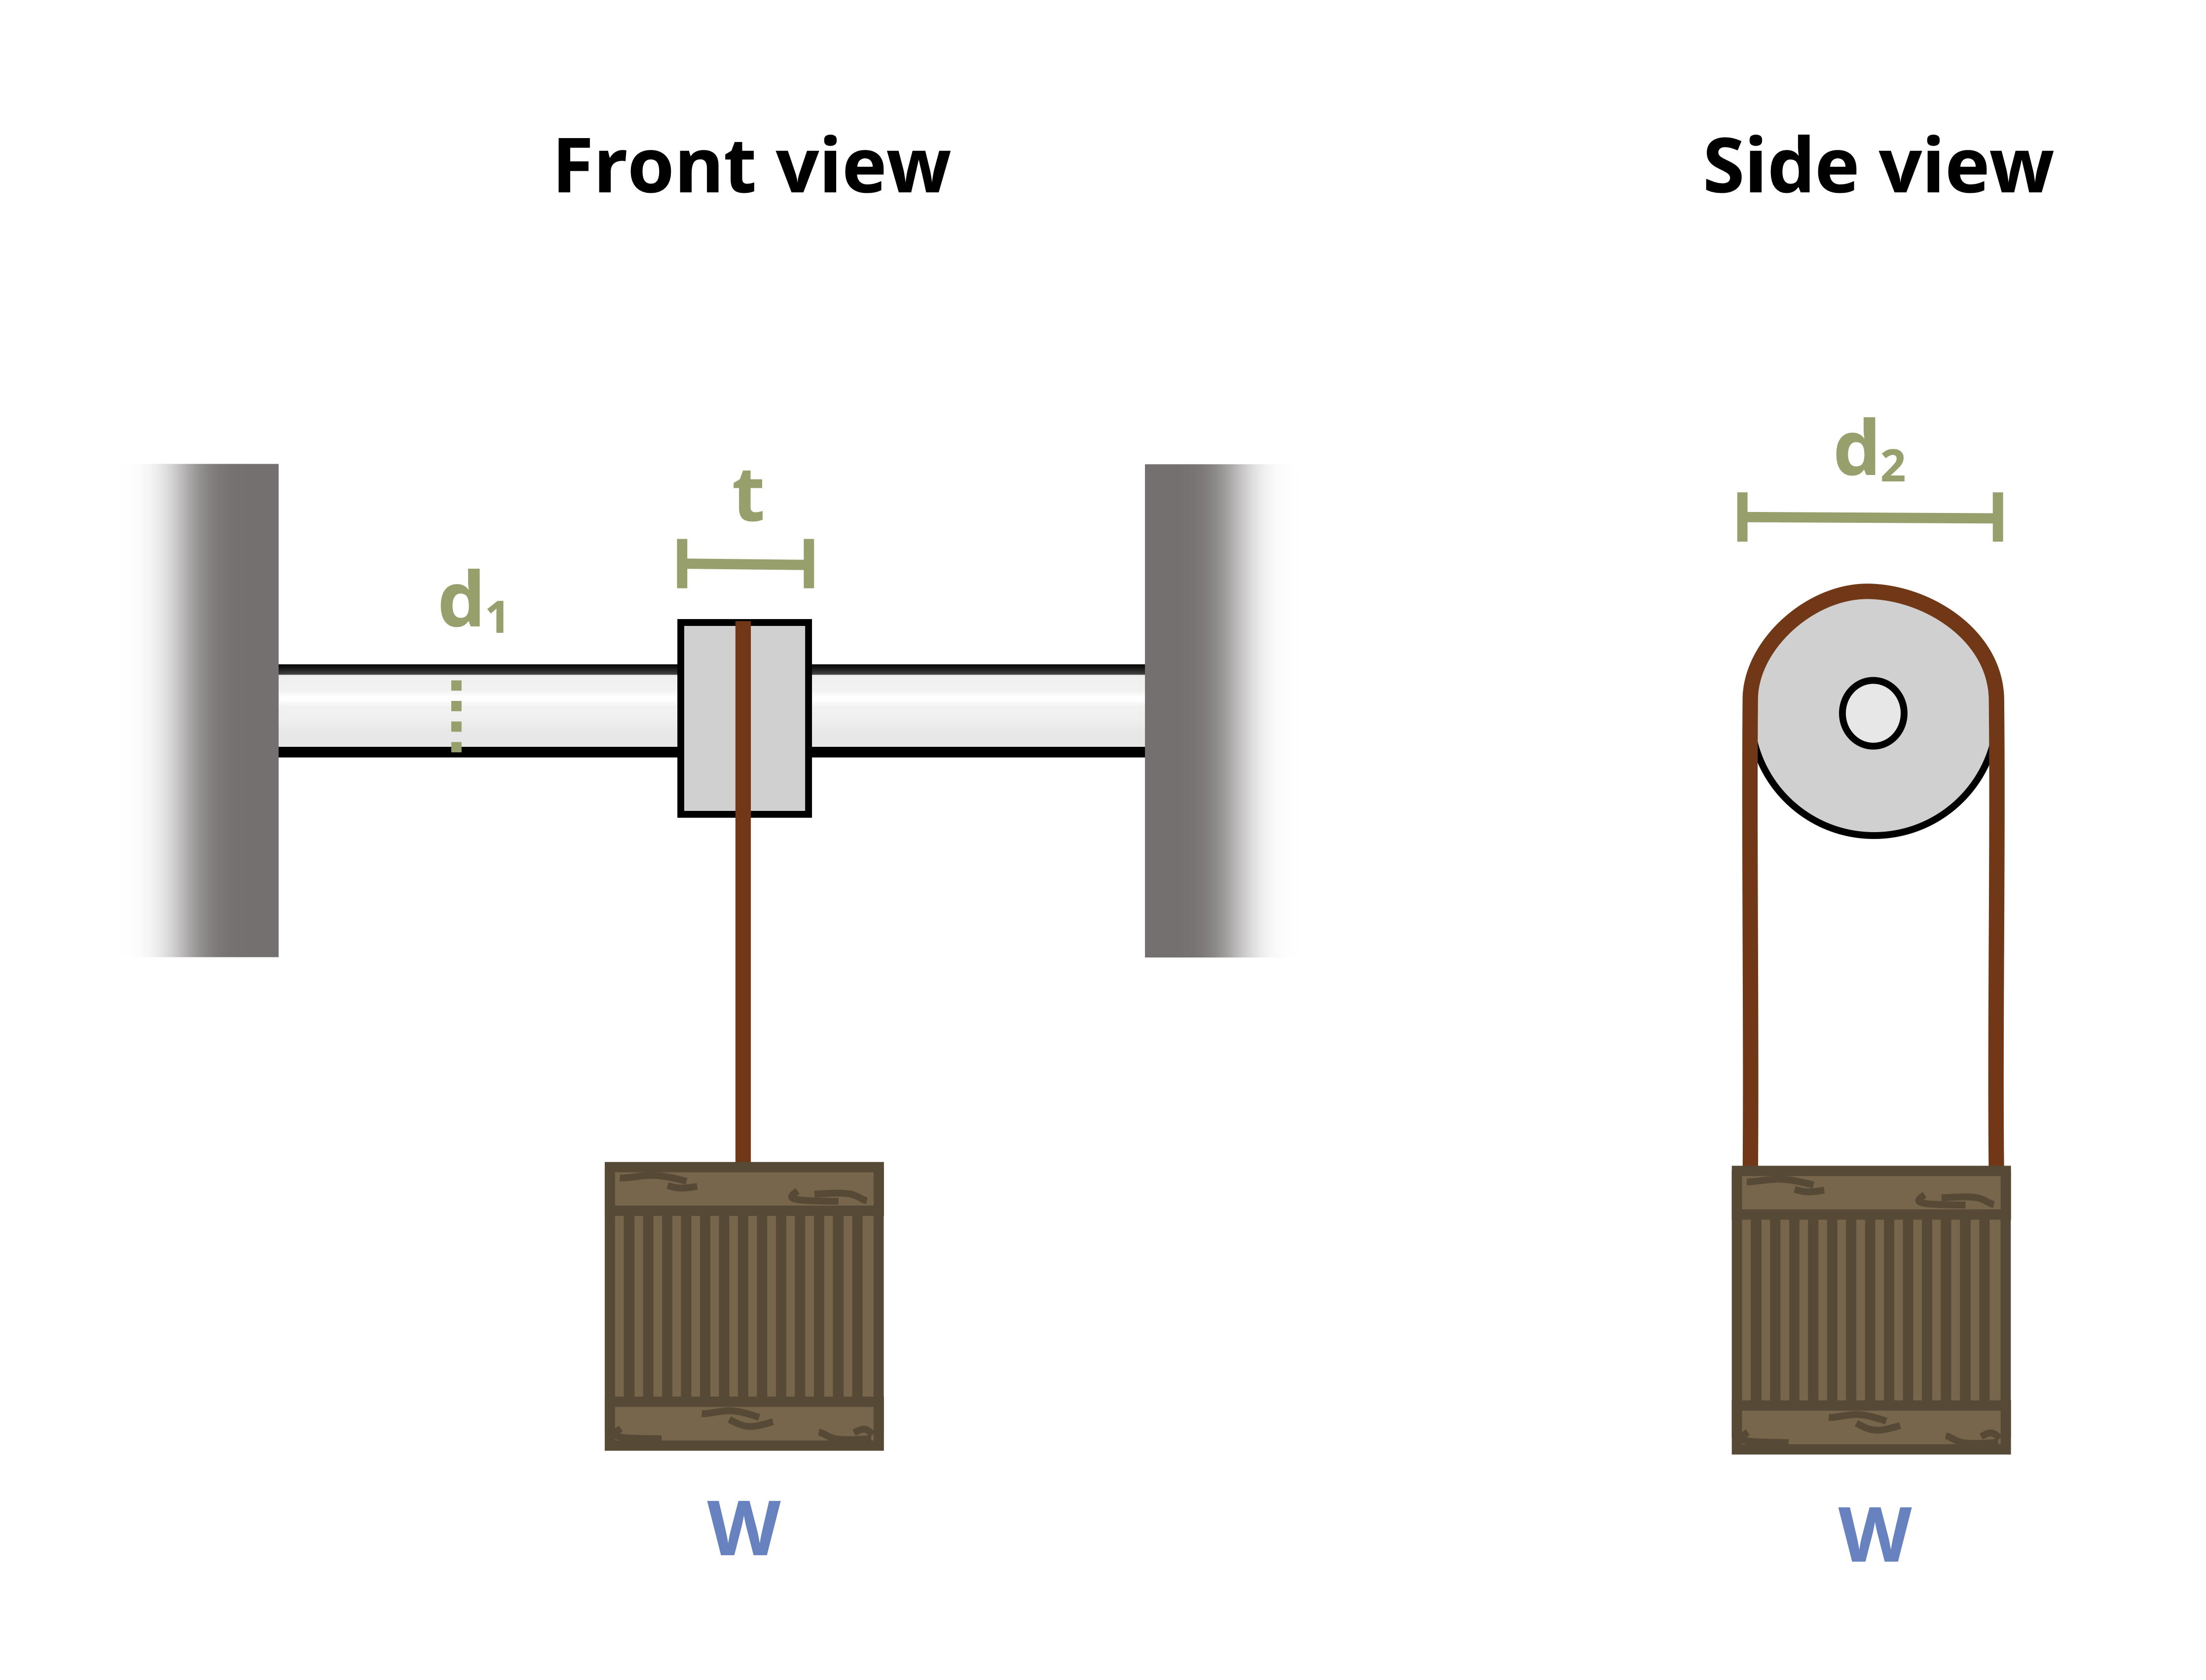
\includegraphics{images/166.png}

}

\caption{Figure 1: A crate is hanged on a circular solid metal rod.}

\end{figure}%

\part{Interactive Interface Demo}

\chapter*{Interactive Problem
Interface}\label{interactive-problem-interface}
\addcontentsline{toc}{chapter}{Interactive Problem Interface}

\markboth{Interactive Problem Interface}{Interactive Problem Interface}

To scaffold your learning in this example, we have provided a free body
diagram for you and a repeat of the problem statement.

A city planner is installing a new traffic light. Light A weighs 65 lb,
while lights B and C weigh 50 lb each. The post at O has a hollow
circular cross-section with an outer diameter of 5 inches and a wall
thickness of 0.2 inches. Please calculate the magnitude of the maximum
combined stress in the post. You may ignore the weight of the post.

\begin{figure}[H]

{\centering 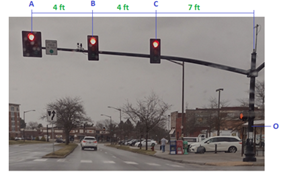
\includegraphics{images/stoplights.png}

}

\caption{Figure 1: Three traffic light installation with loads}

\end{figure}%

Please work through the problem step by step showing your math in the
interactive interface here.

\begin{Shaded}
\begin{Highlighting}[]
\NormalTok{\#| standalone: true}
\NormalTok{\#| viewerHeight: 600}
\NormalTok{\#| components: [viewer]}



\NormalTok{import io}
\NormalTok{import numpy as np}
\NormalTok{import asyncio}
\NormalTok{from datetime import datetime}
\NormalTok{from pathlib import Path}
\NormalTok{import matplotlib.pyplot as plt}
\NormalTok{from shiny import App, render, ui, reactive, req}
\NormalTok{from sympy import solve, Eq, Symbol}
\NormalTok{from sympy.parsing.sympy\_parser import parse\_expr}
\NormalTok{from shiny.ui import h4}

\NormalTok{\# load equations lists}


\NormalTok{class eqn:}
\NormalTok{    def \_\_init\_\_(self, name, inline\_math, newline\_math, working\_sym, working\_eqn\_latex,working\_eqn\_solver):}
\NormalTok{        self.name = name}
\NormalTok{        self.inline\_math = inline\_math}
\NormalTok{        self.newline\_math = newline\_math}
\NormalTok{        self.working\_sym = working\_sym}
\NormalTok{        self.working\_eqn\_latex = working\_eqn\_latex}
\NormalTok{        self.working\_eqn\_solver = working\_eqn\_solver}

\NormalTok{StaticsSumFx = eqn(}
\NormalTok{    "Equilibrium Forces in X", }
\NormalTok{    "\textbackslash{}(\textbackslash{}Sigma F\_x=0\textbackslash{})", }
\NormalTok{    "$$\textbackslash{}Sigma F\_x=0$$", }
\NormalTok{    "SigmaFx",}
\NormalTok{    "$$F\_x1+F\_x2+F\_x3+F\_x4+F\_x5=0$$",}
\NormalTok{    "F\_x1+F\_x2+F\_x3+F\_x4+F\_x5=0"}
\NormalTok{)}

\NormalTok{StaticsSumFy = eqn(}
\NormalTok{    "Equilibrium Forces in Y", }
\NormalTok{    "\textbackslash{}(\textbackslash{}Sigma F\_y=0\textbackslash{})", }
\NormalTok{    "$$\textbackslash{}Sigma F\_y=0$$", }
\NormalTok{    "SigmaFy",}
\NormalTok{    "$$F\_y1+F\_y2+F\_y3+F\_y4+F\_y5=0$$",}
\NormalTok{    "F\_y1+F\_y2+F\_y3+F\_y4+F\_y5=0"}
\NormalTok{)}

\NormalTok{StaticsSumM = eqn(}
\NormalTok{    "Equilibrium Moments about O", }
\NormalTok{    "\textbackslash{}(\textbackslash{}Sigma M\_O=0\textbackslash{})", }
\NormalTok{    "$$\textbackslash{}Sigma M\_O=0$$", }
\NormalTok{    "SigmaM",}
\NormalTok{    "$$M\_1+M\_2+M\_3+M\_4+M\_5=0$$",}
\NormalTok{    "M\_1+M\_2+M\_3+M\_4+M\_5=0"}
\NormalTok{)}

\NormalTok{StressEqn = eqn(}
\NormalTok{    "Stress Equation", }
\NormalTok{    "\textbackslash{}(\textbackslash{}sigma=\textbackslash{}\textbackslash{}frac\{F\}\{A\}\textbackslash{})", }
\NormalTok{    "$$\textbackslash{}sigma=\textbackslash{}\textbackslash{}frac\{F\}\{A\}$$", }
\NormalTok{    "sigma,F,A",}
\NormalTok{    "$$\textbackslash{}sigma=\textbackslash{}\textbackslash{}frac\{(F)\}\{(A)\}$$",}
\NormalTok{    "Eq(sigma,(F)/(A))"}
\NormalTok{)}

\NormalTok{AxialDeform = eqn(}
\NormalTok{    "Axial Deformation by Force",}
\NormalTok{    "\textbackslash{}(\textbackslash{}delta\_l=\textbackslash{}\textbackslash{}frac\{P L\}\{AE\}\textbackslash{})",}
\NormalTok{    "$$\textbackslash{}delta\_l=\textbackslash{}\textbackslash{}frac\{P\textbackslash{}cdot L\}\{A \textbackslash{}cdot E\}$$",}
\NormalTok{    "delta\_l,P,L,A,E",}
\NormalTok{    "$$\textbackslash{}delta\_l=\textbackslash{}\textbackslash{}frac\{(P)(L)\}\{(A)(E)\}$$",}
\NormalTok{    "Eq(delta\_l,(P)*(L)/(A)/(E))"}
\NormalTok{)}

\NormalTok{ThermalDeform = eqn(}
\NormalTok{    "Axial Deformation by Thermal",}
\NormalTok{    "\textbackslash{}(\textbackslash{}delta\_t= \textbackslash{}\textbackslash{}alpha \textbackslash{}Delta T L\textbackslash{})",}
\NormalTok{    "$$\textbackslash{}delta\_t= \textbackslash{}\textbackslash{}alpha \textbackslash{}cdot \textbackslash{}Delta T \textbackslash{}cdot L$$",}
\NormalTok{    "delta\_t,alpha,DeltaT,L",}
\NormalTok{    "$$\textbackslash{}delta\_t= \textbackslash{}\textbackslash{}alpha \textbackslash{}Delta T L$$",}
\NormalTok{    "delta\_t= alpha*(Delta\_T)*L"}
\NormalTok{)}

\NormalTok{AreaTube = eqn(}
\NormalTok{    "Area of a Tube", }
\NormalTok{    "\textbackslash{}(A\_\{tube\}=\textbackslash{}pi(r\_o\^{}2{-}r\_i\^{}2)\textbackslash{})", }
\NormalTok{    "$$A\_\{tube\}=\textbackslash{}pi(r\_o\^{}2{-}r\_i\^{}2)$$", }
\NormalTok{    "A\_tube,r\_o,r\_i",}
\NormalTok{    "$$A\_\{tube\}=\textbackslash{}pi(r\_o\^{}2{-}r\_i\^{}2)$$",}
\NormalTok{    "Eq(A\_tube,pi*((r\_o)**2{-}(r\_i)**2))"}
\NormalTok{)}

\NormalTok{ITube = eqn(}
\NormalTok{    "Moment of Inertia of a Tube",}
\NormalTok{    "\textbackslash{}(I\_\{tube\}=\textbackslash{}\textbackslash{}frac\{\textbackslash{}pi\}\{4\}(r\_o\^{}4{-}r\_i\^{}4)\textbackslash{})",}
\NormalTok{    "$$I\_\{tube\}=\textbackslash{}\textbackslash{}frac\{\textbackslash{}pi\}\{4\}(r\_o\^{}4{-}r\_i\^{}4)$$",}
\NormalTok{    "I\_tube,r\_o,r\_i",}
\NormalTok{    "$$I\_\{tube\}=\textbackslash{}\textbackslash{}frac\{\textbackslash{}pi\}\{4\}(r\_o\^{}4{-}r\_i\^{}4)$$", }
\NormalTok{    "Eq(I\_tube,pi/4*((r\_o)**4{-}(r\_i)**4))" }
\NormalTok{)}

\NormalTok{BendingStress = eqn(}
\NormalTok{    "Bending Stress from a Moment",}
\NormalTok{    "\textbackslash{}(\textbackslash{}sigma\_b=\textbackslash{}\textbackslash{}frac\{M*y\}\{I\}\textbackslash{})",}
\NormalTok{    "$$\textbackslash{}sigma\_b=\textbackslash{}\textbackslash{}frac\{M*y\}\{I\}$$",}
\NormalTok{    "sigma\_b,M,y,I,",}
\NormalTok{    "$$\textbackslash{}sigma\_b=\textbackslash{}\textbackslash{}frac\{M*y\}\{I\}$$", }
\NormalTok{    "Eq(sigma\_b,M*y/I))" }
\NormalTok{)}

\NormalTok{Compatability1 = eqn(}
\NormalTok{    "Compatability Equation 1",}
\NormalTok{    "\textbackslash{}(a\_1+\textbackslash{}ldots=b\_1+b\_2+\textbackslash{}ldots\textbackslash{})", }
\NormalTok{    "$$a\_1+\textbackslash{}ldots=b\_1+b\_2+\textbackslash{}ldots$$", }
\NormalTok{    "",}
\NormalTok{    "$$a\_1+a\_n=b\_1+b\_n$$",}
\NormalTok{    "Eq(a\_1+a\_n=b\_1+b\_n)" }
\NormalTok{)}

\NormalTok{Compatability2 = eqn(}
\NormalTok{    "Compatability Equation 2",}
\NormalTok{    "\textbackslash{}(c\_1+\textbackslash{}ldots=d\_1+d\_2+\textbackslash{}ldots\textbackslash{})", }
\NormalTok{    "$$c\_1+\textbackslash{}ldots=d\_1+d\_2+\textbackslash{}ldots$$", }
\NormalTok{    "",}
\NormalTok{    "$$c\_1+c\_n=d\_1+d\_n$$",}
\NormalTok{    "Eq(c\_1+c\_n=d\_1+d\_n)" }
\NormalTok{)}


\NormalTok{statics\_eqnbank\_inline = \{}
\NormalTok{    StaticsSumFx.name: StaticsSumFx.inline\_math,}
\NormalTok{    StaticsSumFy.name: StaticsSumFy.inline\_math,}
\NormalTok{    StaticsSumM.name: StaticsSumM.inline\_math,}
\NormalTok{\}}
\NormalTok{deforms\_eqnbank\_inline = \{}
\NormalTok{    StressEqn.name: StressEqn.inline\_math,}
\NormalTok{    AxialDeform.name: AxialDeform.inline\_math,}
\NormalTok{    ThermalDeform.name: ThermalDeform.inline\_math,}
\NormalTok{\}}

\NormalTok{geom\_eqnbank\_inline = \{}
\NormalTok{    AreaTube.name: AreaTube.inline\_math,}
\NormalTok{    ITube.name: ITube.inline\_math,}
\NormalTok{\}}

\NormalTok{eqnbank\_inline = \{}
\NormalTok{    StaticsSumFx.name: StaticsSumFx.inline\_math,}
\NormalTok{    StaticsSumFy.name: StaticsSumFy.inline\_math,}
\NormalTok{    StaticsSumM.name: StaticsSumM.inline\_math,}
\NormalTok{    StressEqn.name: StressEqn.inline\_math,}
\NormalTok{    BendingStress.name: BendingStress.inline\_math,}
\NormalTok{    AxialDeform.name: AxialDeform.inline\_math,}
\NormalTok{    ThermalDeform.name: ThermalDeform.inline\_math,}
\NormalTok{    AreaTube.name: AreaTube.inline\_math,}
\NormalTok{    ITube.name: ITube.inline\_math,}
\NormalTok{    Compatability1.name: Compatability1.inline\_math,}
\NormalTok{    Compatability2.name: Compatability2.inline\_math,}
\NormalTok{\}}

\NormalTok{eqnbank\_newline = \{}
\NormalTok{    StaticsSumFx.name: StaticsSumFx.newline\_math,}
\NormalTok{    StaticsSumFy.name: StaticsSumFy.newline\_math,}
\NormalTok{    StaticsSumM.name: StaticsSumM.newline\_math,}
\NormalTok{    StressEqn.name: StressEqn.newline\_math,}
\NormalTok{    BendingStress.name: BendingStress.newline\_math,}
\NormalTok{    AxialDeform.name: AxialDeform.newline\_math,}
\NormalTok{    ThermalDeform.name: ThermalDeform.newline\_math,}
\NormalTok{    AreaTube.name: AreaTube.newline\_math,}
\NormalTok{    ITube.name: ITube.newline\_math,}
\NormalTok{    Compatability1.name: Compatability1.newline\_math,}
\NormalTok{    Compatability2.name: Compatability2.newline\_math,}
\NormalTok{\}}



\NormalTok{working\_equations\_solver=reactive.Value([])}
\NormalTok{working\_equations\_latex\_render=reactive.Value([])}
\NormalTok{working\_symbols=reactive.Value([])}

\NormalTok{feedback\_equations=reactive.Value([])}
\NormalTok{feedback\_solns=reactive.Value([])}
\NormalTok{feedback\_syms=reactive.Value([])}

\NormalTok{working\_SumFx\_render=reactive.Value("")}
\NormalTok{working\_SumFy\_render=reactive.Value("")}
\NormalTok{working\_SumM\_render=reactive.Value("")}
\NormalTok{working\_StressEqn\_render=reactive.Value("")}
\NormalTok{working\_BendingStress\_render=reactive.Value("")}
\NormalTok{working\_AxialDeform\_render=reactive.Value("")}
\NormalTok{working\_ThermalDeform\_render=reactive.Value("")}
\NormalTok{working\_AreaTube\_render=reactive.Value("")}
\NormalTok{working\_Itube\_render=reactive.Value("")}
\NormalTok{working\_Compatability1\_render=reactive.Value("")}
\NormalTok{working\_Compatability2\_render=reactive.Value("")}

\NormalTok{working\_SumFx\_string=reactive.Value("")}
\NormalTok{working\_SumFy\_string=reactive.Value("")}
\NormalTok{working\_SumM\_string=reactive.Value("")}
\NormalTok{working\_StressEqn\_string=reactive.Value("")}
\NormalTok{working\_BendingStress\_string=reactive.Value("")}
\NormalTok{working\_AxialDeform\_string=reactive.Value("")}
\NormalTok{working\_ThermalDeform\_string=reactive.Value("")}
\NormalTok{working\_AreaTube\_string=reactive.Value("")}
\NormalTok{working\_Itube\_string=reactive.Value("")}
\NormalTok{working\_Compatability1\_string=reactive.Value("")}
\NormalTok{working\_Compatability2\_string=reactive.Value("")}

\NormalTok{NumForcesY=reactive.Value(2)}
\NormalTok{F1y=reactive.Value("")}
\NormalTok{F2y=reactive.Value("")}
\NormalTok{F3y=reactive.Value("")}
\NormalTok{F4y=reactive.Value("")}
\NormalTok{F5y=reactive.Value("")}
\NormalTok{Equil\_latex=reactive.Value("")}

\NormalTok{NumForcesX=reactive.Value(2)}
\NormalTok{F1x=reactive.Value("")}
\NormalTok{F2x=reactive.Value("")}
\NormalTok{F3x=reactive.Value("")}
\NormalTok{F4x=reactive.Value("")}
\NormalTok{F5x=reactive.Value("")}

\NormalTok{NumMoments=reactive.Value(2)}
\NormalTok{M1=reactive.Value("")}
\NormalTok{M2=reactive.Value("")}
\NormalTok{M3=reactive.Value("")}
\NormalTok{M4=reactive.Value("")}
\NormalTok{M5=reactive.Value("")}

\NormalTok{axial\_stress\_sigma=reactive.Value("")}
\NormalTok{axial\_stress\_force=reactive.Value("")}
\NormalTok{axial\_stress\_area=reactive.Value("")}

\NormalTok{bending\_stress\_sigma=reactive.Value("")}
\NormalTok{bending\_stress\_M=reactive.Value("")}
\NormalTok{bending\_stress\_y=reactive.Value("")}
\NormalTok{bending\_stress\_I=reactive.Value("")}

\NormalTok{axial\_delta\_l=reactive.Value("")}
\NormalTok{axial\_P=reactive.Value("")}
\NormalTok{axial\_L=reactive.Value("")}
\NormalTok{axial\_A=reactive.Value("")}
\NormalTok{axial\_E=reactive.Value("")}

\NormalTok{thermal\_delta\_t=reactive.Value("")}
\NormalTok{thermal\_alpha=reactive.Value("")}
\NormalTok{thermal\_Delta\_T=reactive.Value("")}
\NormalTok{thermal\_L=reactive.Value("")}

\NormalTok{area\_tube\_A\_tube=reactive.Value("")}
\NormalTok{area\_tube\_Ar\_o=reactive.Value("")}
\NormalTok{area\_tube\_Ar\_i=reactive.Value("")}

\NormalTok{I\_tube\_I\_tube=reactive.Value("")}
\NormalTok{I\_tube\_Ir\_o=reactive.Value("")}
\NormalTok{i\_tube\_Ir\_i=reactive.Value("")}

\NormalTok{Compatability1\_NumLHS=reactive.Value(1)}
\NormalTok{Compatability1\_NumRHS=reactive.Value(2)}
\NormalTok{Compatability1\_a\_1=reactive.Value("")}
\NormalTok{Compatability1\_a\_2=reactive.Value("")}
\NormalTok{Compatability1\_a\_3=reactive.Value("")}
\NormalTok{Compatability1\_a\_4=reactive.Value("")}
\NormalTok{Compatability1\_a\_5=reactive.Value("")}
\NormalTok{Compatability1\_b\_1=reactive.Value("")}
\NormalTok{Compatability1\_b\_2=reactive.Value("")}
\NormalTok{Compatability1\_b\_3=reactive.Value("")}
\NormalTok{Compatability1\_b\_4=reactive.Value("")}
\NormalTok{Compatability1\_b\_5=reactive.Value("")}

\NormalTok{Compatability2\_NumLHS=reactive.Value(1)}
\NormalTok{Compatability2\_NumRHS=reactive.Value(2)}
\NormalTok{Compatability2\_c\_1=reactive.Value("")}
\NormalTok{Compatability2\_c\_2=reactive.Value("")}
\NormalTok{Compatability2\_c\_3=reactive.Value("")}
\NormalTok{Compatability2\_c\_4=reactive.Value("")}
\NormalTok{Compatability2\_c\_5=reactive.Value("")}
\NormalTok{Compatability2\_d\_1=reactive.Value("")}
\NormalTok{Compatability2\_d\_2=reactive.Value("")}
\NormalTok{Compatability2\_d\_3=reactive.Value("")}
\NormalTok{Compatability2\_d\_4=reactive.Value("")}
\NormalTok{Compatability2\_d\_5=reactive.Value("")}

\NormalTok{active\_eqn\_tab=reactive.Value("Instructions")}

\NormalTok{prob\_statement="To scaffold your learning in this example, we have provided a free body diagram for you and a repeat of the problem statement. A city planner is installing a new traffic light. Light A weighs 65 lb, while lights B and C weigh 50 lb each. The post at O has a hollow circular cross{-}section with an outer diameter of 5 inches and a wall thickness of 0.2 inches. Please calculate the magnitude of the maximum combined stress in the post. You may ignore the weight of the post."}

\NormalTok{app\_ui = ui.page\_fluid(}
\NormalTok{    ui.head\_content(}
\NormalTok{        ui.tags.script(}
\NormalTok{            src="https://mathjax.rstudio.com/latest/MathJax.js?config=TeX{-}AMS{-}MML\_HTMLorMML"}
\NormalTok{        ),}
\NormalTok{        ui.tags.script(}
\NormalTok{            "if (window.MathJax) MathJax.Hub.Queue([\textquotesingle{}Typeset\textquotesingle{}, MathJax.Hub]);"}
\NormalTok{        ),}
\NormalTok{    ),}
\NormalTok{    ui.panel\_title("Interactive Problem Solving Environment"),}
\NormalTok{        ui.row(}
\NormalTok{            ui.column(6,}
\NormalTok{                ui.markdown("**Problem Statement**"),}
\NormalTok{                ui.markdown(prob\_statement),}
\NormalTok{                ),}
\NormalTok{            ui.column(6,ui.output\_ui("dyn\_ui\_nav")),}
\NormalTok{            ),}
\NormalTok{        \#ui.row(}
\NormalTok{        \#    ui.output\_ui("dyn\_ui\_nav"),}
\NormalTok{        \#    ),}
\NormalTok{        ui.row(}
\NormalTok{            ui.markdown("**Your Equation Workspace**"),}
\NormalTok{            \#ui.column(6,ui.output\_ui("dyn\_ui\_nav")),}
\NormalTok{            ui.column(4,}
\NormalTok{                ui.navset\_tab\_card(}
\NormalTok{                    ui.nav("Equation Bank",}
\NormalTok{                        ui.input\_checkbox\_group("selected\_eqns","Choose your equations:",eqnbank\_inline,}
\NormalTok{                        ),}
\NormalTok{                    ),}
\NormalTok{                ),}
\NormalTok{            ),}
\NormalTok{            ui.column(2,ui.output\_ui("dyn\_eqns"),style=\textquotesingle{}border{-}right:1px solid;\textquotesingle{}),}
\NormalTok{            ui.column(4,ui.output\_ui("dyn\_working\_eqns"),ui.output\_text("txt")),}
\NormalTok{        ),}
\NormalTok{        ui.row(}
\NormalTok{          ui.output\_ui("ui\_equation\_bookkeeping")}
\NormalTok{        ),}
\NormalTok{        \#ui.row(ui.input\_action\_button(}
\NormalTok{        \#            "solveEquations", "Solve Equations", class\_="btn{-}success", width="240px", style=\textquotesingle{}margin{-}bottom:10px\textquotesingle{})}
\NormalTok{        \#      ),}
\NormalTok{        ui.output\_ui("ui\_solutions"),}
\NormalTok{)}


\NormalTok{def server(input, output, session):}
   
\NormalTok{    @output}
\NormalTok{    @render.ui}
\NormalTok{    def dyn\_eqns():}
\NormalTok{        eqns\_keys = input.selected\_eqns()}
\NormalTok{        req(eqns\_keys)}
\NormalTok{        lookup\_eqns = [eqnbank\_newline[key] for key in eqns\_keys]}
\NormalTok{        mystring\_eqns = "".join(lookup\_eqns)}
\NormalTok{        feedback\_equations.set(lookup\_eqns)}

\NormalTok{        return [}
\NormalTok{            ui.markdown(mystring\_eqns),}
\NormalTok{            ui.tags.script(}
\NormalTok{                "if (window.MathJax) MathJax.Hub.Queue([\textquotesingle{}Typeset\textquotesingle{}, MathJax.Hub]);"}
\NormalTok{            ),}
\NormalTok{        ]}

\NormalTok{    @output}
\NormalTok{    @render.ui}
\NormalTok{    def dyn\_working\_eqns():}
\NormalTok{        eqns\_keys = input.selected\_eqns()}
\NormalTok{        req(eqns\_keys)}
\NormalTok{        lookup\_eqns = [eqnbank\_newline[key] for key in eqns\_keys]}
        

\NormalTok{        \# Dynamic Filling of Force equations }
\NormalTok{        if StaticsSumFy.newline\_math in lookup\_eqns:}
\NormalTok{            StaticsSumFy\_list = ["F\_y1","F\_y2","F\_y3","F\_y4","F\_y5"]}
\NormalTok{            StaticsSumFy\_list = StaticsSumFy\_list[:input.NumForcesY()]}
\NormalTok{            StaticsSumFy.working\_sym = ",".join(StaticsSumFy\_list)}
\NormalTok{            StaticsSumFy.working\_eqn\_latex = "$$" + "+".join(StaticsSumFy\_list) + "=0$$"}
\NormalTok{            StaticsSumFy.working\_eqn\_solver = "+".join(StaticsSumFy\_list)}
            
\NormalTok{            if str(input.F1y()) != "" : }
\NormalTok{                StaticsSumFy.working\_eqn\_latex = StaticsSumFy.working\_eqn\_latex.replace("F\_y1",str(input.F1y()))}
\NormalTok{                StaticsSumFy.working\_sym = StaticsSumFy.working\_sym.replace("F\_y1",str(input.F1y()))}
\NormalTok{                StaticsSumFy.working\_eqn\_solver = StaticsSumFy.working\_eqn\_solver.replace("F\_y1",str(input.F1y()))}
\NormalTok{            else:}
\NormalTok{                StaticsSumFy.working\_eqn\_latex = StaticsSumFy.working\_eqn\_latex.replace("F\_y1","\textbackslash{}\textbackslash{}boxed\{F\_\{y\_1\}\}")}
        
\NormalTok{            if str(input.F2y()) != "" : }
\NormalTok{                StaticsSumFy.working\_eqn\_latex = StaticsSumFy.working\_eqn\_latex.replace("F\_y2",str(input.F2y()))}
\NormalTok{                StaticsSumFy.working\_sym = StaticsSumFy.working\_sym.replace("F\_y2",str(input.F2y()))}
\NormalTok{                StaticsSumFy.working\_eqn\_solver = StaticsSumFy.working\_eqn\_solver.replace("F\_y2",str(input.F2y()))}
\NormalTok{            else:}
\NormalTok{                StaticsSumFy.working\_eqn\_latex = StaticsSumFy.working\_eqn\_latex.replace("F\_y2","\textbackslash{}\textbackslash{}boxed\{F\_\{y\_2\}\}")}
        
\NormalTok{            if str(input.F3y()) != "" : }
\NormalTok{                StaticsSumFy.working\_eqn\_latex = StaticsSumFy.working\_eqn\_latex.replace("F\_y3",str(input.F3y()))}
\NormalTok{                StaticsSumFy.working\_sym = StaticsSumFy.working\_sym.replace("F\_y3",str(input.F3y()))}
\NormalTok{                StaticsSumFy.working\_eqn\_solver = StaticsSumFy.working\_eqn\_solver.replace("F\_y3",str(input.F3y()))}
\NormalTok{            else:}
\NormalTok{                StaticsSumFy.working\_eqn\_latex = StaticsSumFy.working\_eqn\_latex.replace("F\_y3","\textbackslash{}\textbackslash{}boxed\{F\_\{y\_3\}\}")}
        
\NormalTok{            if str(input.F4y()) != "" : }
\NormalTok{                StaticsSumFy.working\_eqn\_latex = StaticsSumFy.working\_eqn\_latex.replace("F\_y4",str(input.F4y()))}
\NormalTok{                StaticsSumFy.working\_sym = StaticsSumFy.working\_sym.replace("F\_y4",str(input.F4y()))}
\NormalTok{                StaticsSumFy.working\_eqn\_solver = StaticsSumFy.working\_eqn\_solver.replace("F\_y4",str(input.F4y()))}
\NormalTok{            else:}
\NormalTok{                StaticsSumFy.working\_eqn\_latex = StaticsSumFy.working\_eqn\_latex.replace("F\_y4","\textbackslash{}\textbackslash{}boxed\{F\_\{y\_4\}\}")}
        
\NormalTok{            if str(input.F5y()) != "" : }
\NormalTok{                StaticsSumFy.working\_eqn\_latex = StaticsSumFy.working\_eqn\_latex.replace("F\_y5",str(input.F5y()))}
\NormalTok{                StaticsSumFy.working\_sym = StaticsSumFy.working\_sym.replace("F\_y5",str(input.F5y()))}
\NormalTok{                StaticsSumFy.working\_eqn\_solver = StaticsSumFy.working\_eqn\_solver.replace("F\_y5",str(input.F5y()))}
\NormalTok{            else:}
\NormalTok{                StaticsSumFy.working\_eqn\_latex = StaticsSumFy.working\_eqn\_latex.replace("F\_y5","\textbackslash{}\textbackslash{}boxed\{F\_\{y\_5\}\}")}
      
\NormalTok{  \# Dynamic Filling of Force equations }
\NormalTok{        if StaticsSumFx.newline\_math in lookup\_eqns:}
\NormalTok{            StaticsSumFx\_list = ["F\_x1","F\_x2","F\_x3","F\_x4","F\_x5"]}
\NormalTok{            StaticsSumFx\_list = StaticsSumFx\_list[:input.NumForcesX()]}
\NormalTok{            StaticsSumFx.working\_sym = ",".join(StaticsSumFx\_list)}
\NormalTok{            StaticsSumFx.working\_eqn\_latex = "$$" + "+".join(StaticsSumFx\_list) + "=0$$"}
\NormalTok{            StaticsSumFx.working\_eqn\_solver = "+".join(StaticsSumFx\_list)}
            
\NormalTok{            if str(input.F1x()) != "" : }
\NormalTok{                StaticsSumFx.working\_eqn\_latex = StaticsSumFx.working\_eqn\_latex.replace("F\_x1",str(input.F1x()))}
\NormalTok{                StaticsSumFx.working\_sym = StaticsSumFx.working\_sym.replace("F\_x1",str(input.F1x()))}
\NormalTok{                StaticsSumFx.working\_eqn\_solver = StaticsSumFx.working\_eqn\_solver.replace("F\_x1",str(input.F1x()))}
\NormalTok{            else:}
\NormalTok{                StaticsSumFx.working\_eqn\_latex = StaticsSumFx.working\_eqn\_latex.replace("F\_x1","\textbackslash{}\textbackslash{}boxed\{F\_\{x\_1\}\}")}
        
\NormalTok{            if str(input.F2x()) != "" : }
\NormalTok{                StaticsSumFx.working\_eqn\_latex = StaticsSumFx.working\_eqn\_latex.replace("F\_x2",str(input.F2x()))}
\NormalTok{                StaticsSumFx.working\_sym = StaticsSumFx.working\_sym.replace("F\_x2",str(input.F2x()))}
\NormalTok{                StaticsSumFx.working\_eqn\_solver = StaticsSumFx.working\_eqn\_solver.replace("F\_x2",str(input.F2x()))}
\NormalTok{            else:}
\NormalTok{                StaticsSumFx.working\_eqn\_latex = StaticsSumFx.working\_eqn\_latex.replace("F\_x2","\textbackslash{}\textbackslash{}boxed\{F\_\{x\_2\}\}")}
        
\NormalTok{            if str(input.F3x()) != "" : }
\NormalTok{                StaticsSumFx.working\_eqn\_latex = StaticsSumFx.working\_eqn\_latex.replace("F\_x3",str(input.F3x()))}
\NormalTok{                StaticsSumFx.working\_sym = StaticsSumFx.working\_sym.replace("F\_x3",str(input.F3x()))}
\NormalTok{                StaticsSumFx.working\_eqn\_solver = StaticsSumFx.working\_eqn\_solver.replace("F\_x3",str(input.F3x()))}
\NormalTok{            else:}
\NormalTok{                StaticsSumFx.working\_eqn\_latex = StaticsSumFx.working\_eqn\_latex.replace("F\_x3","\textbackslash{}\textbackslash{}boxed\{F\_\{x\_3\}\}")}
        
\NormalTok{            if str(input.F4x()) != "" : }
\NormalTok{                StaticsSumFx.working\_eqn\_latex = StaticsSumFx.working\_eqn\_latex.replace("F\_x4",str(input.F4x()))}
\NormalTok{                StaticsSumFx.working\_sym = StaticsSumFx.working\_sym.replace("F\_x4",str(input.F4x()))}
\NormalTok{                StaticsSumFx.working\_eqn\_solver = StaticsSumFx.working\_eqn\_solver.replace("F\_x4",str(input.F4x()))}
\NormalTok{            else:}
\NormalTok{                StaticsSumFx.working\_eqn\_latex = StaticsSumFx.working\_eqn\_latex.replace("F\_x4","\textbackslash{}\textbackslash{}boxed\{F\_\{x\_4\}\}")}
        
\NormalTok{            if str(input.F5x()) != "" : }
\NormalTok{                StaticsSumFx.working\_eqn\_latex = StaticsSumFx.working\_eqn\_latex.replace("F\_x5",str(input.F5x()))}
\NormalTok{                StaticsSumFx.working\_sym = StaticsSumFx.working\_sym.replace("F\_x5",str(input.F5x()))}
\NormalTok{                StaticsSumFx.working\_eqn\_solver = StaticsSumFx.working\_eqn\_solver.replace("F\_x5",str(input.F5x()))}
\NormalTok{            else:}
\NormalTok{                StaticsSumFx.working\_eqn\_latex = StaticsSumFx.working\_eqn\_latex.replace("F\_x5","\textbackslash{}\textbackslash{}boxed\{F\_\{x\_5\}\}")}
                
                
\NormalTok{        \# Dynamic Filling of Moment equations }
\NormalTok{        if StaticsSumM.newline\_math in lookup\_eqns:}
\NormalTok{            StaticsSumM\_list = ["M\_1","M\_2","M\_3","M\_4","M\_5"]}
\NormalTok{            StaticsSumM\_list = StaticsSumM\_list[:input.NumMoments()]}
\NormalTok{            StaticsSumM.working\_sym = ",".join(StaticsSumM\_list)}
\NormalTok{            StaticsSumM.working\_eqn\_latex = "$$" + "+".join(StaticsSumM\_list) + "=0$$"}
\NormalTok{            StaticsSumM.working\_eqn\_solver = "+".join(StaticsSumM\_list)}
            
\NormalTok{            if str(input.M1()) != "" : }
\NormalTok{                StaticsSumM.working\_eqn\_latex = StaticsSumM.working\_eqn\_latex.replace("M\_1",str(input.M1()))}
\NormalTok{                StaticsSumM.working\_sym = StaticsSumM.working\_sym.replace("M\_1",str(input.M1()))}
\NormalTok{                StaticsSumM.working\_eqn\_solver = StaticsSumM.working\_eqn\_solver.replace("M\_1",str(input.M1()))}
\NormalTok{            else:}
\NormalTok{                StaticsSumM.working\_eqn\_latex = StaticsSumM.working\_eqn\_latex.replace("M\_1","\textbackslash{}\textbackslash{}boxed\{M\_1\}")}
        
\NormalTok{            if str(input.M2()) != "" : }
\NormalTok{                StaticsSumM.working\_eqn\_latex = StaticsSumM.working\_eqn\_latex.replace("M\_2",str(input.M2()))}
\NormalTok{                StaticsSumM.working\_sym = StaticsSumM.working\_sym.replace("M\_2",str(input.M2()))}
\NormalTok{                StaticsSumM.working\_eqn\_solver = StaticsSumM.working\_eqn\_solver.replace("M\_2",str(input.M2()))}
\NormalTok{            else:}
\NormalTok{                StaticsSumM.working\_eqn\_latex = StaticsSumM.working\_eqn\_latex.replace("M\_2","\textbackslash{}\textbackslash{}boxed\{M\_2\}")}
        
\NormalTok{            if str(input.M3()) != "" : }
\NormalTok{                StaticsSumM.working\_eqn\_latex = StaticsSumM.working\_eqn\_latex.replace("M\_3",str(input.M3()))}
\NormalTok{                StaticsSumM.working\_sym = StaticsSumM.working\_sym.replace("M\_3",str(input.M3()))}
\NormalTok{                StaticsSumM.working\_eqn\_solver = StaticsSumM.working\_eqn\_solver.replace("M\_3",str(input.M3()))}
\NormalTok{            else:}
\NormalTok{                StaticsSumM.working\_eqn\_latex = StaticsSumM.working\_eqn\_latex.replace("M\_3","\textbackslash{}\textbackslash{}boxed\{M\_3\}")}
        
\NormalTok{            if str(input.M4()) != "" : }
\NormalTok{                StaticsSumM.working\_eqn\_latex = StaticsSumM.working\_eqn\_latex.replace("M\_4",str(input.M4()))}
\NormalTok{                StaticsSumM.working\_sym = StaticsSumM.working\_sym.replace("M\_4",str(input.M4()))}
\NormalTok{                StaticsSumM.working\_eqn\_solver = StaticsSumM.working\_eqn\_solver.replace("M\_4",str(input.M4()))}
\NormalTok{            else:}
\NormalTok{                StaticsSumM.working\_eqn\_latex = StaticsSumM.working\_eqn\_latex.replace("M\_4","\textbackslash{}\textbackslash{}boxed\{M\_4\}")}
        
\NormalTok{            if str(input.M5()) != "" : }
\NormalTok{                StaticsSumM.working\_eqn\_latex = StaticsSumM.working\_eqn\_latex.replace("M\_5",str(input.M5()))}
\NormalTok{                StaticsSumM.working\_sym = StaticsSumM.working\_sym.replace("M\_5",str(input.M5()))}
\NormalTok{                StaticsSumM.working\_eqn\_solver = StaticsSumM.working\_eqn\_solver.replace("M\_5",str(input.M5()))}
\NormalTok{            else:}
\NormalTok{                StaticsSumM.working\_eqn\_latex = StaticsSumM.working\_eqn\_latex.replace("M\_5","\textbackslash{}\textbackslash{}boxed\{M\_5\}")}
          
        
\NormalTok{        \# Dynamic Filling of A equations }
\NormalTok{        if AreaTube.newline\_math in lookup\_eqns:}
\NormalTok{            AreaTube.working\_eqn\_latex = AreaTube.newline\_math}
\NormalTok{            AreaTube.working\_eqn\_solver = "Eq(A\_tube,pi*((r\_o)**2{-}(r\_i)**2))"}
\NormalTok{            AreaTube.working\_sym = "A\_tube,r\_o,r\_i"}
            
\NormalTok{            if str(input.A\_tube()) != "" : }
\NormalTok{                AreaTube.working\_eqn\_latex = AreaTube.working\_eqn\_latex.replace("A\_\{tube\}",str(input.A\_tube()))}
\NormalTok{                AreaTube.working\_sym = AreaTube.working\_sym.replace("A\_tube",str(input.A\_tube()))}
\NormalTok{                AreaTube.working\_eqn\_solver = AreaTube.working\_eqn\_solver.replace("A\_tube",str(input.A\_tube()))}
\NormalTok{            else:}
\NormalTok{                AreaTube.working\_eqn\_latex = AreaTube.working\_eqn\_latex.replace("A\_\{tube\}","\textbackslash{}\textbackslash{}boxed\{A\_\{tube\}\}")}
\NormalTok{            if str(input.Ar\_o()) != "" : }
\NormalTok{                AreaTube.working\_eqn\_latex = AreaTube.working\_eqn\_latex.replace("r\_o",str(input.Ar\_o()))}
\NormalTok{                AreaTube.working\_sym = AreaTube.working\_sym.replace("r\_o",str(input.Ar\_o()))}
\NormalTok{                AreaTube.working\_eqn\_solver = AreaTube.working\_eqn\_solver.replace("r\_o",str(input.Ar\_o()))}
\NormalTok{            else:}
\NormalTok{                AreaTube.working\_eqn\_latex = AreaTube.working\_eqn\_latex.replace("r\_o","\textbackslash{}\textbackslash{}boxed\{r\_o\}")}
\NormalTok{            if str(input.Ar\_i()) != "" : }
\NormalTok{                AreaTube.working\_eqn\_latex = AreaTube.working\_eqn\_latex.replace("r\_i",str(input.Ar\_i()))}
\NormalTok{                AreaTube.working\_sym = AreaTube.working\_sym.replace("r\_i",str(input.Ar\_i()))}
\NormalTok{                AreaTube.working\_eqn\_solver = AreaTube.working\_eqn\_solver.replace("r\_i",str(input.Ar\_i()))}
\NormalTok{            else:}
\NormalTok{                AreaTube.working\_eqn\_latex = AreaTube.working\_eqn\_latex.replace("r\_i","\textbackslash{}\textbackslash{}boxed\{r\_i\}")}
        
\NormalTok{        \# Dynamic Filling of I equations }
\NormalTok{        if ITube.newline\_math in lookup\_eqns:}
\NormalTok{            ITube.working\_eqn\_latex = ITube.newline\_math}
\NormalTok{            ITube.working\_eqn\_solver = "Eq(I\_tube,pi/4*((r\_o)**4{-}(r\_i)**4))"}
\NormalTok{            ITube.working\_sym = "I\_tube,r\_o,r\_i"}
\NormalTok{            if str(input.I\_tube()) != "" : }
\NormalTok{                ITube.working\_eqn\_latex = ITube.working\_eqn\_latex.replace("I\_\{tube\}",str(input.I\_tube()))}
\NormalTok{                ITube.working\_sym = ITube.working\_sym.replace("I\_tube",str(input.I\_tube()))}
\NormalTok{                ITube.working\_eqn\_solver = ITube.working\_eqn\_solver.replace("I\_tube",str(input.I\_tube()))}
\NormalTok{            else:}
\NormalTok{                ITube.working\_eqn\_latex = ITube.working\_eqn\_latex.replace("I\_\{tube\}","\textbackslash{}\textbackslash{}boxed\{I\_\{tube\}\}")}
\NormalTok{            if str(input.Ir\_o()) != "" : }
\NormalTok{                ITube.working\_eqn\_latex = ITube.working\_eqn\_latex.replace("r\_o",str(input.Ir\_o()))}
\NormalTok{                ITube.working\_sym = ITube.working\_sym.replace("r\_o",str(input.Ir\_o()))}
\NormalTok{                ITube.working\_eqn\_solver = ITube.working\_eqn\_solver.replace("r\_o",str(input.Ir\_o()))}
\NormalTok{            else:}
\NormalTok{                ITube.working\_eqn\_latex = ITube.working\_eqn\_latex.replace("r\_o","\textbackslash{}\textbackslash{}boxed\{r\_o\}")}
\NormalTok{            if str(input.Ir\_i()) != "" : }
\NormalTok{                ITube.working\_eqn\_latex = ITube.working\_eqn\_latex.replace("r\_i",str(input.Ir\_i()))        }
\NormalTok{                ITube.working\_sym = ITube.working\_sym.replace("r\_i",str(input.Ir\_i()))}
\NormalTok{                ITube.working\_eqn\_solver = ITube.working\_eqn\_solver.replace("r\_i",str(input.Ir\_i()))}
\NormalTok{            else:}
\NormalTok{                ITube.working\_eqn\_latex = ITube.working\_eqn\_latex.replace("r\_i","\textbackslash{}\textbackslash{}boxed\{r\_i\}")}
            
\NormalTok{        \# Dynamic Filling of Stress equation }
\NormalTok{        if StressEqn.newline\_math in lookup\_eqns:}
\NormalTok{            StressEqn.working\_eqn\_latex = StressEqn.newline\_math}
\NormalTok{            StressEqn.working\_eqn\_solver = "Eq(sigma,(F)/(A))"}
\NormalTok{            StressEqn.working\_sym = "sigma,F,A"}
\NormalTok{            if str(input.sigma()) != "" : }
\NormalTok{                StressEqn.working\_eqn\_latex = StressEqn.working\_eqn\_latex.replace("\textbackslash{}sigma",str(input.sigma()))}
\NormalTok{                StressEqn.working\_eqn\_solver = StressEqn.working\_eqn\_solver.replace("sigma",str(input.sigma()))}
\NormalTok{                StressEqn.working\_sym = StressEqn.working\_sym.replace("sigma",str(input.sigma()))}
\NormalTok{            else:}
\NormalTok{                StressEqn.working\_eqn\_latex = StressEqn.working\_eqn\_latex.replace("\textbackslash{}sigma","\textbackslash{}\textbackslash{}boxed\textbackslash{}sigma")}
\NormalTok{            if str(input.force()) != "" : }
\NormalTok{                StressEqn.working\_eqn\_latex = StressEqn.working\_eqn\_latex.replace("F",str(input.force()))}
\NormalTok{                StressEqn.working\_eqn\_solver = StressEqn.working\_eqn\_solver.replace("F",str(input.force()))}
\NormalTok{                StressEqn.working\_sym = StressEqn.working\_sym.replace("F",str(input.force()))}
\NormalTok{            else:}
\NormalTok{                StressEqn.working\_eqn\_latex = StressEqn.working\_eqn\_latex.replace("F","\textbackslash{}\textbackslash{}boxed\{F\}")}
\NormalTok{            if str(input.area()) != "" : }
\NormalTok{                StressEqn.working\_eqn\_latex = StressEqn.working\_eqn\_latex.replace("A",str(input.area()))}
\NormalTok{                StressEqn.working\_eqn\_solver = StressEqn.working\_eqn\_solver.replace("A",str(input.area()))}
\NormalTok{                StressEqn.working\_sym = StressEqn.working\_sym.replace("A",str(input.area()))}
\NormalTok{            else:}
\NormalTok{                StressEqn.working\_eqn\_latex = StressEqn.working\_eqn\_latex.replace("A","\textbackslash{}\textbackslash{}boxed\{A\}")}
           

\NormalTok{        \# Dynamic Filling of Bending Stress equation }
\NormalTok{        if BendingStress.newline\_math in lookup\_eqns:}
\NormalTok{            BendingStress.working\_eqn\_latex = BendingStress.newline\_math}
\NormalTok{            BendingStress.working\_eqn\_solver = "Eq(sigma\_b,M*y/I)"}
\NormalTok{            BendingStress.working\_sym = "sigma\_b,M,y,I"}
\NormalTok{            if str(input.bendingstress\_sigma\_b()) != "" : }
\NormalTok{                BendingStress.working\_eqn\_latex = BendingStress.working\_eqn\_latex.replace("\textbackslash{}sigma\_b",str(input.bendingstress\_sigma\_b()))}
\NormalTok{                BendingStress.working\_eqn\_solver = BendingStress.working\_eqn\_solver.replace("sigma\_b",str(input.bendingstress\_sigma\_b()))}
\NormalTok{                BendingStress.working\_sym = BendingStress.working\_sym.replace("sigma\_b",str(input.bendingstress\_sigma\_b()))}
\NormalTok{            else:}
\NormalTok{                BendingStress.working\_eqn\_latex = BendingStress.working\_eqn\_latex.replace("\textbackslash{}sigma\_b","\textbackslash{}\textbackslash{}boxed\{\textbackslash{}sigma\_b\}")}
\NormalTok{            if str(input.bendingstress\_M()) != "" : }
\NormalTok{                BendingStress.working\_eqn\_latex = BendingStress.working\_eqn\_latex.replace("M",str(input.bendingstress\_M()))}
\NormalTok{                BendingStress.working\_eqn\_solver = BendingStress.working\_eqn\_solver.replace("M",str(input.bendingstress\_M()))}
\NormalTok{                BendingStress.working\_sym = BendingStress.working\_sym.replace("M",str(input.bendingstress\_M()))}
\NormalTok{            else:}
\NormalTok{                BendingStress.working\_eqn\_latex = BendingStress.working\_eqn\_latex.replace("M","\textbackslash{}\textbackslash{}boxed\{M\}")}
\NormalTok{            if str(input.bendingstress\_y()) != "" : }
\NormalTok{                BendingStress.working\_eqn\_latex = BendingStress.working\_eqn\_latex.replace("y",str(input.bendingstress\_y()))}
\NormalTok{                BendingStress.working\_eqn\_solver = BendingStress.working\_eqn\_solver.replace("y",str(input.bendingstress\_y()))}
\NormalTok{                BendingStress.working\_sym = BendingStress.working\_sym.replace("y",str(input.bendingstress\_y()))}
\NormalTok{            else:}
\NormalTok{                BendingStress.working\_eqn\_latex = BendingStress.working\_eqn\_latex.replace("y","\textbackslash{}\textbackslash{}boxed\{y\}")}
\NormalTok{            if str(input.bendingstress\_I()) != "" : }
\NormalTok{                BendingStress.working\_eqn\_latex = BendingStress.working\_eqn\_latex.replace("I",str(input.bendingstress\_I()))}
\NormalTok{                BendingStress.working\_eqn\_solver = BendingStress.working\_eqn\_solver.replace("I",str(input.bendingstress\_I()))}
\NormalTok{                BendingStress.working\_sym = BendingStress.working\_sym.replace("I",str(input.bendingstress\_I()))}
\NormalTok{            else:}
\NormalTok{                BendingStress.working\_eqn\_latex = BendingStress.working\_eqn\_latex.replace("I","\textbackslash{}\textbackslash{}boxed\{I\}")}
            
                
\NormalTok{        \# Dynamic Filling of Axial Deform equation }
\NormalTok{        if AxialDeform.newline\_math in lookup\_eqns:}
\NormalTok{            AxialDeform.working\_eqn\_latex = AxialDeform.newline\_math}
\NormalTok{            AxialDeform.working\_eqn\_solver = "Eq(delta\_l,P*L/A/E)"}
\NormalTok{            AxialDeform.working\_sym = "delta\_l,P,L,A,E"}
\NormalTok{            if str(input.axial\_delta\_l()) != "" : }
\NormalTok{                AxialDeform.working\_eqn\_latex = AxialDeform.working\_eqn\_latex.replace("\textbackslash{}delta\_l",str(input.axial\_delta\_l()))}
\NormalTok{                AxialDeform.working\_eqn\_solver = AxialDeform.working\_eqn\_solver.replace("delta\_l",str(input.axial\_delta\_l()))}
\NormalTok{                AxialDeform.working\_sym = AxialDeform.working\_sym.replace("delta\_l",str(input.axial\_delta\_l()))}
\NormalTok{            else:}
\NormalTok{                AxialDeform.working\_eqn\_latex = AxialDeform.working\_eqn\_latex.replace("\textbackslash{}delta\_l","\textbackslash{}\textbackslash{}boxed\{\textbackslash{}delta\_l\}")}
\NormalTok{            if str(input.axial\_P()) != "" : }
\NormalTok{                AxialDeform.working\_eqn\_latex = AxialDeform.working\_eqn\_latex.replace("P",str(input.axial\_P()))}
\NormalTok{                AxialDeform.working\_eqn\_solver = AxialDeform.working\_eqn\_solver.replace("P",str(input.axial\_P()))}
\NormalTok{                AxialDeform.working\_sym = AxialDeform.working\_sym.replace("P",str(input.axial\_P()))}
\NormalTok{            else:}
\NormalTok{                AxialDeform.working\_eqn\_latex = AxialDeform.working\_eqn\_latex.replace("P","\textbackslash{}\textbackslash{}boxed\{P\}")}
\NormalTok{            if str(input.axial\_L()) != "" : }
\NormalTok{                AxialDeform.working\_eqn\_latex = AxialDeform.working\_eqn\_latex.replace("L",str(input.axial\_L()))}
\NormalTok{                AxialDeform.working\_eqn\_solver = AxialDeform.working\_eqn\_solver.replace("L",str(input.axial\_L()))}
\NormalTok{                AxialDeform.working\_sym = AxialDeform.working\_sym.replace("L",str(input.axial\_L()))}
\NormalTok{            else:}
\NormalTok{                AxialDeform.working\_eqn\_latex = AxialDeform.working\_eqn\_latex.replace("L","\textbackslash{}\textbackslash{}boxed\{L\}")}
\NormalTok{            if str(input.axial\_A()) != "" : }
\NormalTok{                AxialDeform.working\_eqn\_latex = AxialDeform.working\_eqn\_latex.replace("A",str(input.axial\_A()))}
\NormalTok{                AxialDeform.working\_eqn\_solver = AxialDeform.working\_eqn\_solver.replace("A",str(input.axial\_A()))}
\NormalTok{                AxialDeform.working\_sym = AxialDeform.working\_sym.replace("A",str(input.axial\_A()))}
\NormalTok{            else:}
\NormalTok{                AxialDeform.working\_eqn\_latex = AxialDeform.working\_eqn\_latex.replace("A","\textbackslash{}\textbackslash{}boxed\{A\}")}
\NormalTok{            if str(input.axial\_E()) != "" : }
\NormalTok{                AxialDeform.working\_eqn\_latex = AxialDeform.working\_eqn\_latex.replace("E",str(input.axial\_E()))}
\NormalTok{                AxialDeform.working\_eqn\_solver = AxialDeform.working\_eqn\_solver.replace("E",str(input.axial\_E()))}
\NormalTok{                AxialDeform.working\_sym = AxialDeform.working\_sym.replace("E",str(input.axial\_E()))}
\NormalTok{            else:}
\NormalTok{                AxialDeform.working\_eqn\_latex = AxialDeform.working\_eqn\_latex.replace("E","\textbackslash{}\textbackslash{}boxed\{E\}")}
            
\NormalTok{        \# Dynamic Filling of Thermal Deform equation }
\NormalTok{        if ThermalDeform.newline\_math in lookup\_eqns:}
\NormalTok{            ThermalDeform.working\_eqn\_latex = ThermalDeform.newline\_math}
\NormalTok{            ThermalDeform.working\_eqn\_solver = "Eq(delta\_t,alpha*Delta\_T*L)"}
\NormalTok{            ThermalDeform.working\_sym = "delta\_t,Delta\_T,alpha,L"}
\NormalTok{            if str(input.thermal\_delta\_t()) != "" : }
\NormalTok{                ThermalDeform.working\_eqn\_latex = ThermalDeform.working\_eqn\_latex.replace("\textbackslash{}delta\_t",str(input.thermal\_delta\_t()))}
\NormalTok{                ThermalDeform.working\_eqn\_solver = ThermalDeform.working\_eqn\_solver.replace("delta\_t",str(input.thermal\_delta\_t()))}
\NormalTok{                ThermalDeform.working\_sym = ThermalDeform.working\_sym.replace("delta\_t",str(input.thermal\_delta\_t()))}
\NormalTok{            else:}
\NormalTok{                ThermalDeform.working\_eqn\_latex = ThermalDeform.working\_eqn\_latex.replace("\textbackslash{}delta\_t","\textbackslash{}\textbackslash{}boxed\{\textbackslash{}delta\_t\}")}
\NormalTok{            if str(input.thermal\_alpha()) != "" : }
\NormalTok{                ThermalDeform.working\_eqn\_latex = ThermalDeform.working\_eqn\_latex.replace("\textbackslash{}\textbackslash{}alpha",str(input.thermal\_alpha()))}
\NormalTok{                ThermalDeform.working\_eqn\_solver = ThermalDeform.working\_eqn\_solver.replace("alpha",str(input.thermal\_alpha()))}
\NormalTok{                ThermalDeform.working\_sym = ThermalDeform.working\_sym.replace("alpha",str(input.thermal\_alpha()))}
\NormalTok{            else:}
\NormalTok{                ThermalDeform.working\_eqn\_latex = ThermalDeform.working\_eqn\_latex.replace("\textbackslash{}\textbackslash{}alpha","\textbackslash{}\textbackslash{}boxed\{\textbackslash{}\textbackslash{}alpha\}")}
\NormalTok{            if str(input.thermal\_Delta\_T()) != "" : }
\NormalTok{                ThermalDeform.working\_eqn\_latex = ThermalDeform.working\_eqn\_latex.replace("\textbackslash{}Delta T",str(input.thermal\_Delta\_T()))}
\NormalTok{                ThermalDeform.working\_eqn\_solver = ThermalDeform.working\_eqn\_solver.replace("Delta\_T",str(input.thermal\_Delta\_T()))}
\NormalTok{                ThermalDeform.working\_sym = ThermalDeform.working\_sym.replace("Delta\_T",str(input.thermal\_Delta\_T()))}
\NormalTok{            else:}
\NormalTok{                ThermalDeform.working\_eqn\_latex = ThermalDeform.working\_eqn\_latex.replace("\textbackslash{}Delta T","\textbackslash{}\textbackslash{}boxed\{\textbackslash{}Delta T\}")}
\NormalTok{            if str(input.thermal\_L()) != "" : }
\NormalTok{                ThermalDeform.working\_eqn\_latex = ThermalDeform.working\_eqn\_latex.replace("L",str(input.thermal\_L()))}
\NormalTok{                ThermalDeform.working\_eqn\_solver = ThermalDeform.working\_eqn\_solver.replace("L",str(input.thermal\_L()))}
\NormalTok{                ThermalDeform.working\_sym = ThermalDeform.working\_sym.replace("L",str(input.thermal\_L()))}
\NormalTok{            else:}
\NormalTok{                ThermalDeform.working\_eqn\_latex = ThermalDeform.working\_eqn\_latex.replace("L","\textbackslash{}\textbackslash{}boxed L")}
        
        
\NormalTok{        \# Dynamic Filling of Compatability equation 1 }
\NormalTok{        if Compatability1.newline\_math in lookup\_eqns:}
\NormalTok{            Compatability1\_list\_\_LHS = ["a\_1","a\_2","a\_3","a\_4","a\_5"]}
\NormalTok{            Compatability1\_list\_\_RHS = ["b\_1","b\_2","b\_3","b\_4","b\_5"]}
\NormalTok{            Compatability1\_list\_LHS = Compatability1\_list\_\_LHS[:input.Compatability1\_NumLHS()]}
\NormalTok{            Compatability1\_list\_RHS = Compatability1\_list\_\_RHS[:input.Compatability1\_NumRHS()]}
\NormalTok{            Compatability1\_list = Compatability1\_list\_LHS + Compatability1\_list\_RHS}
\NormalTok{            Compatability1.working\_sym = ",".join(Compatability1\_list)}
\NormalTok{            Compatability1.working\_eqn\_latex = "$$" + "+".join(Compatability1\_list\_LHS) + "=" + "+".join(Compatability1\_list\_RHS)+"$$"}
\NormalTok{            Compatability1.working\_eqn\_solver = "Eq("+ "+".join(Compatability1\_list\_LHS) + "," + "+".join(Compatability1\_list\_RHS)+")"}
            
\NormalTok{            if str(input.a\_1()) != "" : }
\NormalTok{                Compatability1.working\_eqn\_latex = Compatability1.working\_eqn\_latex.replace("a\_1",str(input.a\_1()))}
\NormalTok{                Compatability1.working\_sym = Compatability1.working\_sym.replace("a\_1",str(input.a\_1()))}
\NormalTok{                Compatability1.working\_eqn\_solver = Compatability1.working\_eqn\_solver.replace("a\_1",str(input.a\_1()))}
\NormalTok{            else:}
\NormalTok{                Compatability1.working\_eqn\_latex = Compatability1.working\_eqn\_latex.replace("a\_1","\textbackslash{}\textbackslash{}boxed\{a\_1\}")}
            
\NormalTok{            if str(input.a\_2()) != "" : }
\NormalTok{                Compatability1.working\_eqn\_latex = Compatability1.working\_eqn\_latex.replace("a\_2",str(input.a\_2()))}
\NormalTok{                Compatability1.working\_sym = Compatability1.working\_sym.replace("a\_2",str(input.a\_2()))}
\NormalTok{                Compatability1.working\_eqn\_solver = Compatability1.working\_eqn\_solver.replace("a\_2",str(input.a\_2()))}
\NormalTok{            else:}
\NormalTok{                Compatability1.working\_eqn\_latex = Compatability1.working\_eqn\_latex.replace("a\_2","\textbackslash{}\textbackslash{}boxed\{a\_2\}")}
            
\NormalTok{            if str(input.a\_3()) != "" : }
\NormalTok{                Compatability1.working\_eqn\_latex = Compatability1.working\_eqn\_latex.replace("a\_3",str(input.a\_3()))}
\NormalTok{                Compatability1.working\_sym = Compatability1.working\_sym.replace("a\_3",str(input.a\_3()))}
\NormalTok{                Compatability1.working\_eqn\_solver = Compatability1.working\_eqn\_solver.replace("a\_3",str(input.a\_3()))}
\NormalTok{            else:}
\NormalTok{                Compatability1.working\_eqn\_latex = Compatability1.working\_eqn\_latex.replace("a\_3","\textbackslash{}\textbackslash{}boxed\{a\_3\}")}
            
\NormalTok{            if str(input.a\_4()) != "" : }
\NormalTok{                Compatability1.working\_eqn\_latex = Compatability1.working\_eqn\_latex.replace("a\_4",str(input.a\_4()))}
\NormalTok{                Compatability1.working\_sym = Compatability1.working\_sym.replace("a\_4",str(input.a\_4()))}
\NormalTok{                Compatability1.working\_eqn\_solver = Compatability1.working\_eqn\_solver.replace("a\_4",str(input.a\_4()))}
\NormalTok{            else:}
\NormalTok{                Compatability1.working\_eqn\_latex = Compatability1.working\_eqn\_latex.replace("a\_4","\textbackslash{}\textbackslash{}boxed\{a\_4\}")}
            
\NormalTok{            if str(input.a\_5()) != "" : }
\NormalTok{                Compatability1.working\_eqn\_latex = Compatability1.working\_eqn\_latex.replace("a\_5",str(input.a\_5()))}
\NormalTok{                Compatability1.working\_sym = Compatability1.working\_sym.replace("a\_5",str(input.a\_5()))}
\NormalTok{                Compatability1.working\_eqn\_solver = Compatability1.working\_eqn\_solver.replace("a\_5",str(input.a\_5()))}
\NormalTok{            else:}
\NormalTok{                Compatability1.working\_eqn\_latex = Compatability1.working\_eqn\_latex.replace("a\_5","\textbackslash{}\textbackslash{}boxed\{a\_5\}")}
                    
\NormalTok{            if str(input.b\_1()) != "" : }
\NormalTok{                Compatability1.working\_eqn\_latex = Compatability1.working\_eqn\_latex.replace("b\_1",str(input.b\_1()))}
\NormalTok{                Compatability1.working\_sym = Compatability1.working\_sym.replace("b\_1",str(input.b\_1()))}
\NormalTok{                Compatability1.working\_eqn\_solver = Compatability1.working\_eqn\_solver.replace("b\_1",str(input.b\_1()))}
\NormalTok{            else:}
\NormalTok{                Compatability1.working\_eqn\_latex = Compatability1.working\_eqn\_latex.replace("b\_1","\textbackslash{}\textbackslash{}boxed\{b\_1\}")}
            
\NormalTok{            if str(input.b\_2()) != "" : }
\NormalTok{                Compatability1.working\_eqn\_latex = Compatability1.working\_eqn\_latex.replace("b\_2",str(input.b\_2()))}
\NormalTok{                Compatability1.working\_sym = Compatability1.working\_sym.replace("b\_2",str(input.b\_2()))}
\NormalTok{                Compatability1.working\_eqn\_solver = Compatability1.working\_eqn\_solver.replace("b\_2",str(input.b\_2()))}
\NormalTok{            else:}
\NormalTok{                Compatability1.working\_eqn\_latex = Compatability1.working\_eqn\_latex.replace("b\_2","\textbackslash{}\textbackslash{}boxed\{b\_2\}")}
            
\NormalTok{            if str(input.b\_3()) != "" : }
\NormalTok{                Compatability1.working\_eqn\_latex = Compatability1.working\_eqn\_latex.replace("b\_3",str(input.b\_3()))}
\NormalTok{                Compatability1.working\_sym = Compatability1.working\_sym.replace("b\_3",str(input.b\_3()))}
\NormalTok{                Compatability1.working\_eqn\_solver = Compatability1.working\_eqn\_solver.replace("b\_3",str(input.b\_3()))}
\NormalTok{            else:}
\NormalTok{                Compatability1.working\_eqn\_latex = Compatability1.working\_eqn\_latex.replace("b\_3","\textbackslash{}\textbackslash{}boxed\{b\_3\}")}
            
\NormalTok{            if str(input.b\_4()) != "" : }
\NormalTok{                Compatability1.working\_eqn\_latex = Compatability1.working\_eqn\_latex.replace("b\_4",str(input.b\_4()))}
\NormalTok{                Compatability1.working\_sym = Compatability1.working\_sym.replace("b\_4",str(input.b\_4()))}
\NormalTok{                Compatability1.working\_eqn\_solver = Compatability1.working\_eqn\_solver.replace("b\_4",str(input.b\_4()))}
\NormalTok{            else:}
\NormalTok{                Compatability1.working\_eqn\_latex = Compatability1.working\_eqn\_latex.replace("b\_4","\textbackslash{}\textbackslash{}boxed\{b\_4\}")}
            
\NormalTok{            if str(input.b\_5()) != "" : }
\NormalTok{                Compatability1.working\_eqn\_latex = Compatability1.working\_eqn\_latex.replace("b\_5",str(input.b\_5()))}
\NormalTok{                Compatability1.working\_sym = Compatability1.working\_sym.replace("b\_5",str(input.b\_5()))}
\NormalTok{                Compatability1.working\_eqn\_solver = Compatability1.working\_eqn\_solver.replace("b\_5",str(input.b\_5()))}
\NormalTok{            else:}
\NormalTok{                Compatability1.working\_eqn\_latex = Compatability1.working\_eqn\_latex.replace("b\_5","\textbackslash{}\textbackslash{}boxed\{b\_5\}")}

\NormalTok{\# Dynamic Filling of Compatability equation 2}
\NormalTok{        if Compatability2.newline\_math in lookup\_eqns:}
\NormalTok{            Compatability2\_list\_\_LHS = ["c\_1","c\_2","c\_3","c\_4","c\_5"]}
\NormalTok{            Compatability2\_list\_\_RHS = ["d\_1","d\_2","d\_3","d\_4","d\_5"]}
\NormalTok{            Compatability2\_list\_LHS = Compatability2\_list\_\_LHS[:input.Compatability2\_NumLHS()]}
\NormalTok{            Compatability2\_list\_RHS = Compatability2\_list\_\_RHS[:input.Compatability2\_NumRHS()]}
\NormalTok{            Compatability2\_list = Compatability2\_list\_LHS + Compatability2\_list\_RHS}
\NormalTok{            Compatability2.working\_sym = ",".join(Compatability2\_list)}
\NormalTok{            Compatability2.working\_eqn\_latex = "$$" + "+".join(Compatability2\_list\_LHS) + "=" + "+".join(Compatability2\_list\_RHS)+"$$"}
\NormalTok{            Compatability2.working\_eqn\_solver = "Eq("+ "+".join(Compatability2\_list\_LHS) + "," + "+".join(Compatability2\_list\_RHS)+")"}
            
\NormalTok{            if str(input.c\_1()) != "" : }
\NormalTok{                Compatability2.working\_eqn\_latex = Compatability2.working\_eqn\_latex.replace("c\_1",str(input.c\_1()))}
\NormalTok{                Compatability2.working\_sym = Compatability2.working\_sym.replace("c\_1",str(input.c\_1()))}
\NormalTok{                Compatability2.working\_eqn\_solver = Compatability2.working\_eqn\_solver.replace("c\_1",str(input.c\_1()))}
\NormalTok{            else:}
\NormalTok{                Compatability2.working\_eqn\_latex = Compatability2.working\_eqn\_latex.replace("c\_1","\textbackslash{}\textbackslash{}boxed\{c\_1\}")}
            
\NormalTok{            if str(input.c\_2()) != "" : }
\NormalTok{                Compatability2.working\_eqn\_latex = Compatability2.working\_eqn\_latex.replace("c\_2",str(input.c\_2()))}
\NormalTok{                Compatability2.working\_sym = Compatability2.working\_sym.replace("c\_2",str(input.c\_2()))}
\NormalTok{                Compatability2.working\_eqn\_solver = Compatability2.working\_eqn\_solver.replace("c\_2",str(input.c\_2()))}
\NormalTok{            else:}
\NormalTok{                Compatability2.working\_eqn\_latex = Compatability2.working\_eqn\_latex.replace("c\_2","\textbackslash{}\textbackslash{}boxed\{c\_2\}")}
            
\NormalTok{            if str(input.c\_3()) != "" : }
\NormalTok{                Compatability2.working\_eqn\_latex = Compatability2.working\_eqn\_latex.replace("c\_3",str(input.c\_3()))}
\NormalTok{                Compatability2.working\_sym = Compatability2.working\_sym.replace("c\_3",str(input.c\_3()))}
\NormalTok{                Compatability2.working\_eqn\_solver = Compatability2.working\_eqn\_solver.replace("c\_3",str(input.c\_3()))}
\NormalTok{            else:}
\NormalTok{                Compatability2.working\_eqn\_latex = Compatability2.working\_eqn\_latex.replace("c\_3","\textbackslash{}\textbackslash{}boxed\{c\_3\}")}
            
\NormalTok{            if str(input.c\_4()) != "" : }
\NormalTok{                Compatability2.working\_eqn\_latex = Compatability2.working\_eqn\_latex.replace("c\_4",str(input.c\_4()))}
\NormalTok{                Compatability2.working\_sym = Compatability2.working\_sym.replace("c\_4",str(input.c\_4()))}
\NormalTok{                Compatability2.working\_eqn\_solver = Compatability2.working\_eqn\_solver.replace("c\_4",str(input.c\_4()))}
\NormalTok{            else:}
\NormalTok{                Compatability2.working\_eqn\_latex = Compatability2.working\_eqn\_latex.replace("c\_4","\textbackslash{}\textbackslash{}boxed\{c\_4\}")}
            
\NormalTok{            if str(input.c\_5()) != "" : }
\NormalTok{                Compatability2.working\_eqn\_latex = Compatability2.working\_eqn\_latex.replace("c\_5",str(input.c\_5()))}
\NormalTok{                Compatability2.working\_sym = Compatability2.working\_sym.replace("c\_5",str(input.c\_5()))}
\NormalTok{                Compatability2.working\_eqn\_solver = Compatability2.working\_eqn\_solver.replace("c\_5",str(input.c\_5()))}
\NormalTok{            else:}
\NormalTok{                Compatability2.working\_eqn\_latex = Compatability2.working\_eqn\_latex.replace("c\_5","\textbackslash{}\textbackslash{}boxed\{c\_5\}")}
                    
\NormalTok{            if str(input.d\_1()) != "" : }
\NormalTok{                Compatability2.working\_eqn\_latex = Compatability2.working\_eqn\_latex.replace("d\_1",str(input.d\_1()))}
\NormalTok{                Compatability2.working\_sym = Compatability2.working\_sym.replace("d\_1",str(input.d\_1()))}
\NormalTok{                Compatability2.working\_eqn\_solver = Compatability2.working\_eqn\_solver.replace("d\_1",str(input.d\_1()))}
\NormalTok{            else:}
\NormalTok{                Compatability2.working\_eqn\_latex = Compatability2.working\_eqn\_latex.replace("d\_1","\textbackslash{}\textbackslash{}boxed\{d\_1\}")}
            
\NormalTok{            if str(input.d\_2()) != "" : }
\NormalTok{                Compatability2.working\_eqn\_latex = Compatability2.working\_eqn\_latex.replace("d\_2",str(input.d\_2()))}
\NormalTok{                Compatability2.working\_sym = Compatability2.working\_sym.replace("d\_2",str(input.d\_2()))}
\NormalTok{                Compatability2.working\_eqn\_solver = Compatability2.working\_eqn\_solver.replace("d\_2",str(input.d\_2()))}
\NormalTok{            else:}
\NormalTok{                Compatability2.working\_eqn\_latex = Compatability2.working\_eqn\_latex.replace("d\_2","\textbackslash{}\textbackslash{}boxed\{d\_2\}")}
            
\NormalTok{            if str(input.d\_3()) != "" : }
\NormalTok{                Compatability2.working\_eqn\_latex = Compatability2.working\_eqn\_latex.replace("d\_3",str(input.d\_3()))}
\NormalTok{                Compatability2.working\_sym = Compatability2.working\_sym.replace("d\_3",str(input.d\_3()))}
\NormalTok{                Compatability2.working\_eqn\_solver = Compatability2.working\_eqn\_solver.replace("d\_3",str(input.d\_3()))}
\NormalTok{            else:}
\NormalTok{                Compatability2.working\_eqn\_latex = Compatability2.working\_eqn\_latex.replace("d\_3","\textbackslash{}\textbackslash{}boxed\{d\_3\}")}
            
\NormalTok{            if str(input.d\_4()) != "" : }
\NormalTok{                Compatability2.working\_eqn\_latex = Compatability2.working\_eqn\_latex.replace("d\_4",str(input.d\_4()))}
\NormalTok{                Compatability2.working\_sym = Compatability2.working\_sym.replace("d\_4",str(input.d\_4()))}
\NormalTok{                Compatability2.working\_eqn\_solver = Compatability2.working\_eqn\_solver.replace("d\_4",str(input.d\_4()))}
\NormalTok{            else:}
\NormalTok{                Compatability2.working\_eqn\_latex = Compatability2.working\_eqn\_latex.replace("d\_4","\textbackslash{}\textbackslash{}boxed\{d\_4\}")}
            
\NormalTok{            if str(input.d\_5()) != "" : }
\NormalTok{                Compatability2.working\_eqn\_latex = Compatability2.working\_eqn\_latex.replace("d\_5",str(input.d\_5()))}
\NormalTok{                Compatability2.working\_sym = Compatability2.working\_sym.replace("d\_5",str(input.d\_5()))}
\NormalTok{                Compatability2.working\_eqn\_solver = Compatability2.working\_eqn\_solver.replace("d\_5",str(input.d\_5()))}
\NormalTok{            else:}
\NormalTok{                Compatability2.working\_eqn\_latex = Compatability2.working\_eqn\_latex.replace("d\_5","\textbackslash{}\textbackslash{}boxed\{d\_5\}")}
                
                
\NormalTok{        eqnbank\_working\_latex = \{}
\NormalTok{        StaticsSumFx.name: StaticsSumFx.working\_eqn\_latex,}
\NormalTok{        StaticsSumFy.name: StaticsSumFy.working\_eqn\_latex,}
\NormalTok{        StaticsSumM.name: StaticsSumM.working\_eqn\_latex,}
\NormalTok{        StressEqn.name: StressEqn.working\_eqn\_latex,}
\NormalTok{        BendingStress.name: BendingStress.working\_eqn\_latex,}
\NormalTok{        AxialDeform.name: AxialDeform.working\_eqn\_latex,}
\NormalTok{        ThermalDeform.name: ThermalDeform.working\_eqn\_latex,}
\NormalTok{        AreaTube.name: AreaTube.working\_eqn\_latex,}
\NormalTok{        ITube.name: ITube.working\_eqn\_latex,}
\NormalTok{        Compatability1.name: Compatability1.working\_eqn\_latex,}
\NormalTok{        Compatability2.name: Compatability2.working\_eqn\_latex}
\NormalTok{        \}}

\NormalTok{        eqnbank\_working\_solver = \{}
\NormalTok{        StaticsSumFx.name: StaticsSumFx.working\_eqn\_solver,}
\NormalTok{        StaticsSumFy.name: StaticsSumFy.working\_eqn\_solver,}
\NormalTok{        StaticsSumM.name: StaticsSumM.working\_eqn\_solver,}
\NormalTok{        StressEqn.name: StressEqn.working\_eqn\_solver,}
\NormalTok{        BendingStress.name: BendingStress.working\_eqn\_solver,}
\NormalTok{        AxialDeform.name: AxialDeform.working\_eqn\_solver,}
\NormalTok{        ThermalDeform.name: ThermalDeform.working\_eqn\_solver,}
\NormalTok{        AreaTube.name: AreaTube.working\_eqn\_solver,}
\NormalTok{        ITube.name: ITube.working\_eqn\_solver,}
\NormalTok{        Compatability1.name: Compatability1.working\_eqn\_solver,}
\NormalTok{        Compatability2.name: Compatability2.working\_eqn\_solver}
\NormalTok{        \}}

\NormalTok{        symbank\_working = \{}
\NormalTok{        StaticsSumFx.name: StaticsSumFx.working\_sym,}
\NormalTok{        StaticsSumFy.name: StaticsSumFy.working\_sym,}
\NormalTok{        StaticsSumM.name: StaticsSumM.working\_sym,}
\NormalTok{        StressEqn.name: StressEqn.working\_sym,}
\NormalTok{        BendingStress.name: BendingStress.working\_sym,}
\NormalTok{        AxialDeform.name: AxialDeform.working\_sym,}
\NormalTok{        ThermalDeform.name: ThermalDeform.working\_sym,}
\NormalTok{        AreaTube.name: AreaTube.working\_sym,}
\NormalTok{        ITube.name: ITube.working\_sym,}
\NormalTok{        Compatability1.name: Compatability1.working\_sym,}
\NormalTok{        Compatability2.name: Compatability2.working\_sym}
\NormalTok{        \}}
        
\NormalTok{        working\_eqns\_latex = [eqnbank\_working\_latex[key] for key in eqns\_keys]}
\NormalTok{        working\_SumFx\_render.set(eqnbank\_working\_latex["Equilibrium Forces in X"])}
\NormalTok{        working\_SumFy\_render.set(eqnbank\_working\_latex["Equilibrium Forces in Y"])}
\NormalTok{        working\_SumM\_render.set(eqnbank\_working\_latex["Equilibrium Moments about O"])}
\NormalTok{        working\_StressEqn\_render.set(eqnbank\_working\_latex["Stress Equation"])}
\NormalTok{        working\_BendingStress\_render.set(eqnbank\_working\_latex["Bending Stress from a Moment"])}
\NormalTok{        working\_AxialDeform\_render.set(eqnbank\_working\_latex["Axial Deformation by Force"])}
\NormalTok{        working\_ThermalDeform\_render.set(eqnbank\_working\_latex["Axial Deformation by Thermal"])}
\NormalTok{        working\_AreaTube\_render.set(eqnbank\_working\_latex["Area of a Tube"])}
\NormalTok{        working\_Itube\_render.set(eqnbank\_working\_latex["Moment of Inertia of a Tube"])}
\NormalTok{        working\_Compatability1\_render.set(eqnbank\_working\_latex["Compatability Equation 1"])}
\NormalTok{        working\_Compatability2\_render.set(eqnbank\_working\_latex["Compatability Equation 2"])}
\NormalTok{        working\_eqns\_solver = [eqnbank\_working\_solver[key] for key in eqns\_keys]}
        
\NormalTok{        temp\_working\_equations\_solver = "\#".join(working\_eqns\_solver)}
\NormalTok{        temp\_working\_equations\_solver = temp\_working\_equations\_solver.replace("Eq","Wrap\_clash")}
\NormalTok{        temp\_working\_equations\_solver = temp\_working\_equations\_solver.replace("E","E\_clash")}
\NormalTok{        temp\_working\_equations\_solver = temp\_working\_equations\_solver.replace("I","I\_clash")}
\NormalTok{        temp\_working\_equations\_solver = temp\_working\_equations\_solver.replace("N","N\_clash")}
\NormalTok{        temp\_working\_equations\_solver = temp\_working\_equations\_solver.replace("Wrap\_clash","Eq")}
\NormalTok{        working\_eqns\_solver = temp\_working\_equations\_solver.split("\#")}
        
\NormalTok{        \#working\_eqns\_solver=[]}
\NormalTok{        \#for j in working\_eqns\_solver\_pre:}
\NormalTok{        \#    temp=j.split(",")}
\NormalTok{        \#    temp2=temp.replace("I","I\_clash")}
\NormalTok{        \#    temp3=temp2.replace("E","E\_clash")}
\NormalTok{        \#    working\_eqns\_solver.append(temp3)}
        
\NormalTok{        working\_syms = [symbank\_working[key] for key in eqns\_keys]}
\NormalTok{        mystring\_working\_eqns = "".join(working\_eqns\_latex)}
\NormalTok{        mystring\_working\_eqns = mystring\_working\_eqns.replace("*","\textbackslash{}\textbackslash{}times")}
\NormalTok{        feedback\_syms.set(working\_syms)}
\NormalTok{        working\_equations\_solver.set(working\_eqns\_solver)}

\NormalTok{        working\_syms\_only=[]}
\NormalTok{        for j in working\_syms:}
\NormalTok{            temp=j.split(",")}
\NormalTok{            for k in temp:}
\NormalTok{                try: }
\NormalTok{                    float(eval(k))  }
\NormalTok{                except:}
\NormalTok{                    temp2=k.replace("I","I\_clash")}
\NormalTok{                    temp3=temp2.replace("E","E\_clash")}
\NormalTok{                    temp4=temp3.replace("N","N\_clash")}
\NormalTok{                    working\_syms\_only.append(temp4)}
\NormalTok{        working\_syms\_only=list(dict.fromkeys(working\_syms\_only))}
\NormalTok{        working\_symbols.set(working\_syms\_only)}
        
\NormalTok{        return [}
\NormalTok{            ui.markdown(mystring\_working\_eqns),}
\NormalTok{            ui.tags.script(}
\NormalTok{                "if (window.MathJax) MathJax.Hub.Queue([\textquotesingle{}Typeset\textquotesingle{}, MathJax.Hub]);"}
\NormalTok{            )}
\NormalTok{        ]}
    
\NormalTok{    @output}
\NormalTok{    @render.ui}
\NormalTok{    def dyn\_ui\_nav():}
      
\NormalTok{        tab\_Instructions = ui.nav(}
\NormalTok{            "Instructions",ui.markdown("Please choose the equations you would like to use in this problem. As you do, tabs will load here which allow you to browse between active equations and define the necessary parameters or variables to set up your solution. As you fill in parameters and variables, the working palette will change to reflect what values you are plugging in and will give you a running update of the number of equations you have relative to the number of unknowns you have. A solve equations button will be available for when you are ready to solve and the system will provide the solution to your system of equations. \textless{}br\textgreater{} \textless{}br\textgreater{} Note: You may put in simple math into the blanks (e.g., 3*4 instead of 12) which can be helpful in specifying Moment values or performing unit conversions in place. At this time, you may not mix and match this math with variables (e.g., typing in 5x in the blank will not parse the 5 as a number and the x as a variable) \textless{}br\textgreater{} \textless{}br\textgreater{} Key issues still needing development include: support for units?, **FEEDBACK**, choosing a solution value from the solution set, parameterized problem statement values...") }
\NormalTok{        )}
    
\NormalTok{        tab\_StaticsSumFy = ui.nav(}
\NormalTok{                str(StaticsSumFy.inline\_math),}
\NormalTok{                \#ui.markdown(working\_SumFy\_string()),}
\NormalTok{                ui.input\_numeric("NumForcesY","How many terms do you want?",value=NumForcesY(),min=2,max=5),}
\NormalTok{                ui.input\_text("F1y","\textbackslash{}(F\_\{y\_1\}=\textbackslash{})", value=F1y(),placeholder="Please type in variable or value"),}
\NormalTok{                ui.input\_text("F2y","\textbackslash{}(F\_\{y\_2\}=\textbackslash{})", value=F2y(),placeholder="Please type in variable or value"),}
\NormalTok{                ui.panel\_conditional("input.NumForcesY\textgreater{}=3", ui.input\_text("F3y","\textbackslash{}(F\_\{y\_3\}=\textbackslash{})", value=F3y(),placeholder="Please type in variable or value")),}
\NormalTok{                ui.panel\_conditional("input.NumForcesY\textgreater{}=4", ui.input\_text("F4y","\textbackslash{}(F\_\{y\_4\}=\textbackslash{})", value=F4y(),placeholder="Please type in variable or value")),}
\NormalTok{                ui.panel\_conditional("input.NumForcesY\textgreater{}=5", ui.input\_text("F5y","\textbackslash{}(F\_\{y\_5\}=\textbackslash{})", value=F5y(),placeholder="Please type in variable or value"))}
\NormalTok{                )}
        
\NormalTok{        tab\_StaticsSumFx = ui.nav(}
\NormalTok{                str(StaticsSumFx.inline\_math),}
\NormalTok{                \#ui.markdown(working\_SumFx\_string()),}
\NormalTok{                ui.input\_numeric("NumForcesX","How many terms do you want?",value=NumForcesX(),min=2,max=5),}
\NormalTok{                ui.input\_text("F1x","\textbackslash{}(F\_\{x\_1\}=\textbackslash{})", value=F1x(),placeholder="Please type in variable or value"),}
\NormalTok{                ui.input\_text("F2x","\textbackslash{}(F\_\{x\_2\}=\textbackslash{})", value=F2x(),placeholder="Please type in variable or value"),}
\NormalTok{                ui.panel\_conditional("input.NumForcesX\textgreater{}=3", ui.input\_text("F3x","\textbackslash{}(F\_\{x\_3\}=\textbackslash{})", value=F3x(),placeholder="Please type in variable or value")),}
\NormalTok{                ui.panel\_conditional("input.NumForcesX\textgreater{}=4", ui.input\_text("F4x","\textbackslash{}(F\_\{x\_4\}=\textbackslash{})", value=F4x(),placeholder="Please type in variable or value")),}
\NormalTok{                ui.panel\_conditional("input.NumForcesX\textgreater{}=5", ui.input\_text("F5x","\textbackslash{}(F\_\{x\_5\}=\textbackslash{})", value=F5x(),placeholder="Please type in variable or value"))}
\NormalTok{                )}
        
\NormalTok{        tab\_StaticsSumM = ui.nav(}
\NormalTok{                str(StaticsSumM.inline\_math),}
\NormalTok{                \#ui.markdown(working\_SumM\_string()),}
\NormalTok{                ui.input\_numeric("NumMoments","How many terms do you want?",value=NumMoments(),min=2,max=5),}
\NormalTok{                ui.input\_text("M1","\textbackslash{}(M\_1=\textbackslash{})", value=M1(),placeholder="Please type in variables, values, or numeric math (e.g., (3*4))"),}
\NormalTok{                ui.input\_text("M2","\textbackslash{}(M\_2=\textbackslash{})", value=M2(),placeholder="Please type in variables, values, or numeric math (e.g., (3*4))"),}
\NormalTok{                ui.panel\_conditional("input.NumMoments\textgreater{}=3", ui.input\_text("M3","\textbackslash{}(M\_3=\textbackslash{})", value=M3(),placeholder="Please type in variable, values, or numeric math (e.g., (3*4))")),}
\NormalTok{                ui.panel\_conditional("input.NumMoments\textgreater{}=4", ui.input\_text("M4","\textbackslash{}(M\_4=\textbackslash{})", value=M4(),placeholder="Please type in variable , values, or numeric math (e.g., (3*4))")),}
\NormalTok{                ui.panel\_conditional("input.NumMoments\textgreater{}=5", ui.input\_text("M5","\textbackslash{}(M\_5=\textbackslash{})", value=M5(),placeholder="Please type in variable , values, or numeric math (e.g., (3*4))"))}
\NormalTok{                )}
        
\NormalTok{        tab\_StressEqn = ui.nav(}
\NormalTok{                str(StressEqn.inline\_math),}
\NormalTok{                \#ui.markdown(working\_StressEqn\_string()),}
\NormalTok{                ui.input\_text("sigma","\textbackslash{}(\textbackslash{}sigma\textbackslash{})", value=axial\_stress\_sigma(),placeholder="Please type in variables or values"),}
\NormalTok{                ui.input\_text("force","\textbackslash{}(F\textbackslash{})", value=axial\_stress\_force(),placeholder="Please type in variables or values"),}
\NormalTok{                ui.input\_text("area","\textbackslash{}(A\textbackslash{})", value=axial\_stress\_area(),placeholder="Please type in variables or values"),}
\NormalTok{                )}
        
\NormalTok{        tab\_BendingStress = ui.nav(}
\NormalTok{                str(BendingStress.inline\_math),}
\NormalTok{                \#ui.markdown(working\_BendingStress\_string()),}
\NormalTok{                ui.input\_text("bendingstress\_sigma\_b","\textbackslash{}(\textbackslash{}sigma\_b\textbackslash{})", value=bending\_stress\_sigma(), placeholder="Please type in variables or values"),}
\NormalTok{                ui.input\_text("bendingstress\_M","\textbackslash{}(M\textbackslash{})", value=bending\_stress\_M(), placeholder="Please type in variables or values"),}
\NormalTok{                ui.input\_text("bendingstress\_y","\textbackslash{}(y\textbackslash{})", value=bending\_stress\_y(), placeholder="Please type in variables or values"),}
\NormalTok{                ui.input\_text("bendingstress\_I","\textbackslash{}(I\textbackslash{})", value= bending\_stress\_I(), placeholder="Please type in variables or values"),}
\NormalTok{                )}
        
\NormalTok{        tab\_AxialDeform = ui.nav(}
\NormalTok{                str(AxialDeform.inline\_math),}
\NormalTok{                \#ui.markdown(working\_AxialDeform\_string()),}
\NormalTok{                ui.input\_text("axial\_delta\_l","\textbackslash{}(\textbackslash{}delta\_l\textbackslash{})", value=axial\_delta\_l(), placeholder="Please type in variables or values"),}
\NormalTok{                ui.input\_text("axial\_P","\textbackslash{}(P\textbackslash{})", value=axial\_P(), placeholder="Please type in variables or values"),}
\NormalTok{                ui.input\_text("axial\_L","\textbackslash{}(L\textbackslash{})", value=axial\_L(), placeholder="Please type in variables or values"),}
\NormalTok{                ui.input\_text("axial\_A","\textbackslash{}(A\textbackslash{})", value=axial\_A(), placeholder="Please type in variables or values"),}
\NormalTok{                ui.input\_text("axial\_E","\textbackslash{}(E\textbackslash{})", value=axial\_E(), placeholder="Please type in variables or values"),}
\NormalTok{                )}
        
\NormalTok{        tab\_ThermalDeform = ui.nav(}
\NormalTok{                str(ThermalDeform.inline\_math),}
\NormalTok{                \#ui.markdown(working\_ThermalDeform\_string()),}
\NormalTok{                ui.input\_text("thermal\_delta\_t","\textbackslash{}(\textbackslash{}delta\_t\textbackslash{})", value=thermal\_delta\_t(), placeholder="Please type in variables or values"),}
\NormalTok{                ui.input\_text("thermal\_alpha","\textbackslash{}(\textbackslash{}\textbackslash{}alpha\textbackslash{})", value=thermal\_alpha(), placeholder="Please type in variables or values"),}
\NormalTok{                ui.input\_text("thermal\_Delta\_T","\textbackslash{}(\textbackslash{}Delta T\textbackslash{})", value=thermal\_Delta\_T(), placeholder="Please type in variables or values"),}
\NormalTok{                ui.input\_text("thermal\_L","\textbackslash{}(L\textbackslash{})", value=thermal\_L(), placeholder="Please type in variables or values"),}
\NormalTok{                )}
        
\NormalTok{        tab\_AreaTube = ui.nav(}
\NormalTok{                str(AreaTube.inline\_math),}
\NormalTok{                \#ui.markdown(working\_AreaTube\_string()),}
\NormalTok{                ui.input\_text("A\_tube","\textbackslash{}(A\_\{tube\}=\textbackslash{})", value=area\_tube\_A\_tube(), placeholder="Please type in variables or values"),}
\NormalTok{                ui.input\_text("Ar\_o","\textbackslash{}(r\_o=\textbackslash{})", value=area\_tube\_Ar\_o(), placeholder="Please type in variables or values"),}
\NormalTok{                ui.input\_text("Ar\_i","\textbackslash{}(r\_i\textbackslash{})", value=area\_tube\_Ar\_i(), placeholder="Please type in variables or values")}
\NormalTok{                )}
        
\NormalTok{        tab\_ITube = ui.nav(}
\NormalTok{                str(ITube.inline\_math),}
\NormalTok{                \#ui.markdown(working\_Itube\_string()),}
\NormalTok{                ui.input\_text("I\_tube","\textbackslash{}(I\_\{tube\}=\textbackslash{})", value=I\_tube\_I\_tube(), placeholder="Please type in variables or values"),}
\NormalTok{                ui.input\_text("Ir\_o","\textbackslash{}(r\_o=\textbackslash{})", value=I\_tube\_Ir\_o(), placeholder="Please type in variables or values"),}
\NormalTok{                ui.input\_text("Ir\_i","\textbackslash{}(r\_i\textbackslash{})", value=i\_tube\_Ir\_i(), placeholder="Please type in variables or values"),}
\NormalTok{                )}
        
\NormalTok{        tab\_Compatability1 = ui.nav(}
\NormalTok{                str(Compatability1.inline\_math),}
\NormalTok{                \#ui.markdown(working\_Compatability1\_string()),}
\NormalTok{                ui.input\_numeric("Compatability1\_NumLHS","How many \textquotesingle{}a\textquotesingle{} terms do you want?",value=Compatability1\_NumLHS(),min=1,max=5),}
\NormalTok{                ui.input\_numeric("Compatability1\_NumRHS","How many \textquotesingle{}b\textquotesingle{} terms do you want?",value=Compatability1\_NumRHS(),min=1,max=5),}
\NormalTok{                ui.input\_text("a\_1","\textbackslash{}(a\_1=\textbackslash{})", value=Compatability1\_a\_1(),placeholder="Please type in variable or value"),}
\NormalTok{                ui.panel\_conditional("input.Compatability1\_NumLHS\textgreater{}=2",ui.input\_text("a\_2","\textbackslash{}(a\_2=\textbackslash{})", value=Compatability1\_a\_2(),placeholder="Please type in variable or value")),}
\NormalTok{                ui.panel\_conditional("input.Compatability1\_NumLHS\textgreater{}=3", ui.input\_text("a\_3","\textbackslash{}(a\_3=\textbackslash{})", value=Compatability1\_a\_3(),placeholder="Please type in variable or value")),}
\NormalTok{                ui.panel\_conditional("input.Compatability1\_NumLHS\textgreater{}=4", ui.input\_text("a\_4","\textbackslash{}(a\_4=\textbackslash{})", value=Compatability1\_a\_4(),placeholder="Please type in variable or value")),}
\NormalTok{                ui.panel\_conditional("input.Compatability1\_NumLHS\textgreater{}=5", ui.input\_text("a\_5","\textbackslash{}(a\_5=\textbackslash{})", value=Compatability1\_a\_5(),placeholder="Please type in variable or value")),}
\NormalTok{                ui.input\_text("b\_1","\textbackslash{}(b\_1=\textbackslash{})", value=Compatability1\_b\_1(),placeholder="Please type in variable or value"),}
\NormalTok{                ui.panel\_conditional("input.Compatability1\_NumRHS\textgreater{}=2",ui.input\_text("b\_2","\textbackslash{}(b\_2=\textbackslash{})", value=Compatability1\_b\_2(),placeholder="Please type in variable or value")),}
\NormalTok{                ui.panel\_conditional("input.Compatability1\_NumRHS\textgreater{}=3",ui.input\_text("b\_3","\textbackslash{}(b\_3=\textbackslash{})", value=Compatability1\_b\_3(),placeholder="Please type in variable or value")),}
\NormalTok{                ui.panel\_conditional("input.Compatability1\_NumRHS\textgreater{}=4",ui.input\_text("b\_4","\textbackslash{}(b\_4=\textbackslash{})", value=Compatability1\_b\_4(),placeholder="Please type in variable or value")),}
\NormalTok{                ui.panel\_conditional("input.Compatability1\_NumRHS\textgreater{}=5",ui.input\_text("b\_5","\textbackslash{}(b\_5=\textbackslash{})", value=Compatability1\_b\_5(),placeholder="Please type in variable or value")),}
\NormalTok{                )}
        
\NormalTok{        tab\_Compatability2 = ui.nav(}
\NormalTok{                str(Compatability2.inline\_math),}
\NormalTok{                \#ui.markdown(working\_Compatability2\_string()),}
\NormalTok{                ui.input\_numeric("Compatability2\_NumLHS","How many \textquotesingle{}c\textquotesingle{} terms do you want?",value=Compatability2\_NumLHS(),min=1,max=5),}
\NormalTok{                ui.input\_numeric("Compatability2\_NumRHS","How many \textquotesingle{}d\textquotesingle{} terms do you want?",value=Compatability2\_NumRHS(),min=1,max=5),}
\NormalTok{                ui.input\_text("c\_1","\textbackslash{}(c\_1=\textbackslash{})", value=Compatability2\_c\_1(),placeholder="Please type in variable or value"),}
\NormalTok{                ui.panel\_conditional("input.Compatability2\_NumLHS\textgreater{}=2",ui.input\_text("c\_2","\textbackslash{}(c\_2=\textbackslash{})", value=Compatability2\_c\_2(),placeholder="Please type in variable or value")),}
\NormalTok{                ui.panel\_conditional("input.Compatability2\_NumLHS\textgreater{}=3", ui.input\_text("c\_3","\textbackslash{}(c\_3=\textbackslash{})", value=Compatability2\_c\_3(),placeholder="Please type in variable or value")),}
\NormalTok{                ui.panel\_conditional("input.Compatability2\_NumLHS\textgreater{}=4", ui.input\_text("c\_4","\textbackslash{}(c\_4=\textbackslash{})", value=Compatability2\_c\_4(),placeholder="Please type in variable or value")),}
\NormalTok{                ui.panel\_conditional("input.Compatability2\_NumLHS\textgreater{}=5", ui.input\_text("c\_5","\textbackslash{}(c\_5=\textbackslash{})", value=Compatability2\_c\_5(),placeholder="Please type in variable or value")),}
\NormalTok{                ui.input\_text("d\_1","\textbackslash{}(d\_1=\textbackslash{})", value=Compatability2\_d\_1(),placeholder="Please type in variable or value"),}
\NormalTok{                ui.panel\_conditional("input.Compatability2\_NumRHS\textgreater{}=2",ui.input\_text("d\_2","\textbackslash{}(d\_2=\textbackslash{})", value=Compatability2\_d\_2(),placeholder="Please type in variable or value")),}
\NormalTok{                ui.panel\_conditional("input.Compatability2\_NumRHS\textgreater{}=3",ui.input\_text("d\_3","\textbackslash{}(d\_3=\textbackslash{})", value=Compatability2\_d\_3(),placeholder="Please type in variable or value")),}
\NormalTok{                ui.panel\_conditional("input.Compatability2\_NumRHS\textgreater{}=4",ui.input\_text("d\_4","\textbackslash{}(d\_4=\textbackslash{})", value=Compatability2\_d\_4(),placeholder="Please type in variable or value")),}
\NormalTok{                ui.panel\_conditional("input.Compatability2\_NumRHS\textgreater{}=5",ui.input\_text("d\_5","\textbackslash{}(d\_5=\textbackslash{})", value=Compatability2\_d\_5(),placeholder="Please type in variable or value")),}
\NormalTok{                )}

\NormalTok{        tab\_bank = \{}
\NormalTok{                StaticsSumFx.name: tab\_StaticsSumFx,}
\NormalTok{                StaticsSumFy.name: tab\_StaticsSumFy,}
\NormalTok{                StaticsSumM.name: tab\_StaticsSumM,}
\NormalTok{                StressEqn.name: tab\_StressEqn,}
\NormalTok{                BendingStress.name: tab\_BendingStress,}
\NormalTok{                AxialDeform.name: tab\_AxialDeform,}
\NormalTok{                ThermalDeform.name: tab\_ThermalDeform,}
\NormalTok{                AreaTube.name: tab\_AreaTube,}
\NormalTok{                ITube.name: tab\_ITube,}
\NormalTok{                Compatability1.name: tab\_Compatability1,}
\NormalTok{                Compatability2.name: tab\_Compatability2,}
\NormalTok{                \}}
\NormalTok{        eqns\_keys = input.selected\_eqns()}
\NormalTok{        tabs = [tab\_bank[key] for key in eqns\_keys]}
\NormalTok{        tabs.insert(0,tab\_Instructions)}
\NormalTok{        equations = ui.navset\_tab\_card(*tabs,id="mytab",selected=active\_eqn\_tab())                    }
    
\NormalTok{        return [equations,}
\NormalTok{               ui.tags.script(}
\NormalTok{                "if (window.MathJax) MathJax.Hub.Queue([\textquotesingle{}Typeset\textquotesingle{}, MathJax.Hub]);"}
\NormalTok{        ),]}

\NormalTok{    @output}
\NormalTok{    @render.ui}
\NormalTok{    def ui\_equation\_bookkeeping():}
\NormalTok{        req(working\_equations\_solver())}
\NormalTok{        num\_working\_equations=len(working\_equations\_solver())}
\NormalTok{        num\_working\_symbols=len(working\_symbols())}
\NormalTok{        string\_working\_symbols= "\textbackslash{}\textbackslash{}\textbackslash{}\textbackslash{}("+"\textbackslash{}\textbackslash{}\textbackslash{}\textbackslash{}),\textbackslash{}\textbackslash{}\textbackslash{}\textbackslash{}(".join(working\_symbols())+"\textbackslash{}\textbackslash{}\textbackslash{}\textbackslash{})"}
\NormalTok{        string\_working\_symbols=string\_working\_symbols.replace("N\_clash","N")}
\NormalTok{        string\_working\_symbols=string\_working\_symbols.replace("I\_clash","I")}
\NormalTok{        string\_working\_symbols=string\_working\_symbols.replace("E\_clash","E")}
\NormalTok{        string\_working\_symbols=string\_working\_symbols.replace("delta","\textbackslash{}delta")}
\NormalTok{        string\_working\_symbols=string\_working\_symbols.replace("Delta","\textbackslash{}Delta")}
\NormalTok{        string\_working\_symbols=string\_working\_symbols.replace("sigma","\textbackslash{}sigma")}
\NormalTok{        return [ui.markdown(f"Your equation{-}solver set up currently has **\{num\_working\_equations\} equations** and **\{num\_working\_symbols\} unknowns**. \textless{}br\textgreater{}  Your current unknowns are \{string\_working\_symbols\}"), }
\NormalTok{                ui.input\_action\_button(}
\NormalTok{                    "solveEquations", "Solve Equations", class\_="btn{-}success", width="240px", style=\textquotesingle{}margin{-}bottom:10px\textquotesingle{}),}
\NormalTok{                ui.tags.script(}
\NormalTok{                "if (window.MathJax) MathJax.Hub.Queue([\textquotesingle{}Typeset\textquotesingle{}, MathJax.Hub]);"}
\NormalTok{                )]}
        
\NormalTok{    @output}
\NormalTok{    @render.ui}
\NormalTok{    @reactive.event(input.solveEquations)}
\NormalTok{    def ui\_solutions():}
\NormalTok{        for j in working\_symbols():}
\NormalTok{            j=Symbol(j)}
\NormalTok{        print(working\_equations\_solver())}
\NormalTok{        print(working\_symbols())}
\NormalTok{        my\_solver\_equations=[]}
\NormalTok{        for m in working\_equations\_solver():}
\NormalTok{            m=parse\_expr(m)}
\NormalTok{        solve\_eqns = solve(working\_equations\_solver(),working\_symbols(),dict=True)}
\NormalTok{        answers=[]}
\NormalTok{        for k in working\_symbols():}
\NormalTok{            try: }
\NormalTok{                temp=solve\_eqns[0][parse\_expr(k)]}
\NormalTok{                temp2="$$"+k+"="+f\textquotesingle{}\{temp:.2f\}\textquotesingle{}+"$$"}
\NormalTok{                answers.append(temp2)}
\NormalTok{            except:}
\NormalTok{                pass}
\NormalTok{        mystring\_answers="".join(answers)}
\NormalTok{        mystring\_answers=mystring\_answers.replace("pi","\textbackslash{}pi")}
\NormalTok{        mystring\_answers=mystring\_answers.replace("delta","\textbackslash{}delta")}
\NormalTok{        mystring\_answers=mystring\_answers.replace("Delta","\textbackslash{}Delta")}
\NormalTok{        mystring\_answers=mystring\_answers.replace("sigma","\textbackslash{}sigma")}
\NormalTok{        mystring\_answers=mystring\_answers.replace("E\_clash","E")}
\NormalTok{        mystring\_answers=mystring\_answers.replace("I\_clash","I")}
\NormalTok{        mystring\_answers=mystring\_answers.replace("N\_clash","N")}
\NormalTok{        \#feedback\_solns.set(mystring\_answers)}
\NormalTok{        return [ui.markdown(f"Your solution is \{mystring\_answers\}"),}
\NormalTok{                ui.input\_text("answer","Answer:",placeholder="Please type in your answer"),}
\NormalTok{                ui.input\_action\_button("feedback", "Check answer and show feedback"),}
\NormalTok{                ui.download\_button("download", "Download File to Submit", class\_="btn{-}success"),}
\NormalTok{                ui.tags.script(}
\NormalTok{                "if (window.MathJax) MathJax.Hub.Queue([\textquotesingle{}Typeset\textquotesingle{}, MathJax.Hub]);"}
\NormalTok{                )]}

\NormalTok{    \#@reactive.Effect}
\NormalTok{    \#def \_():}

\NormalTok{     \#   active\_eqn\_tab.set(input.mytab())}
    
    
\NormalTok{    @reactive.Effect}
\NormalTok{    def \_():}

\NormalTok{        input.selected\_eqns()}
\NormalTok{        active\_eqn\_tab.set(input.mytab())}
        
        
\NormalTok{        \#working\_SumFx\_render():}
\NormalTok{        \#working\_SumFy\_render()}
\NormalTok{        \#working\_SumM\_render()}
\NormalTok{        \#working\_StressEqn\_render()}
\NormalTok{        \#working\_BendingStress\_render()}
\NormalTok{        \#working\_AxialDeform\_render()}
\NormalTok{        \#working\_ThermalDeform\_render()}
\NormalTok{        \#working\_AreaTube\_render()}
\NormalTok{        \#working\_Itube\_render()}
\NormalTok{        \#working\_Compatability1\_render()}
\NormalTok{        \#working\_Compatability2\_render()}
                
\NormalTok{        with reactive.isolate():}
\NormalTok{            if "Equilibrium Forces in Y" in input.selected\_eqns(): }
\NormalTok{                NumForcesY.set(input.NumForcesY())}
\NormalTok{                F1y.set(input.F1y())}
\NormalTok{                F2y.set(input.F2y())}
\NormalTok{                F3y.set(input.F3y())}
\NormalTok{                F4y.set(input.F4y())}
\NormalTok{                F5y.set(input.F5y())}
\NormalTok{                working\_SumFy\_string.set(str(working\_SumFy\_render()))}
\NormalTok{            else:}
\NormalTok{                 pass             }
    
\NormalTok{            if "Equilibrium Forces in X" in input.selected\_eqns(): }
\NormalTok{                NumForcesX.set(input.NumForcesX())}
\NormalTok{                F1x.set(input.F1x())}
\NormalTok{                F2x.set(input.F2x())}
\NormalTok{                F3x.set(input.F3x())}
\NormalTok{                F4x.set(input.F4x())}
\NormalTok{                F5x.set(input.F5x())}
\NormalTok{                working\_SumFx\_string.set(str(working\_SumFx\_render()))}
\NormalTok{            else:}
\NormalTok{                 pass}
                              
\NormalTok{            if "Equilibrium Moments about O" in input.selected\_eqns(): }
\NormalTok{                NumMoments.set(input.NumMoments())}
\NormalTok{                M1.set(input.M1())}
\NormalTok{                M2.set(input.M2())}
\NormalTok{                M3.set(input.M3())}
\NormalTok{                M4.set(input.M4())}
\NormalTok{                M5.set(input.M5())}
\NormalTok{                working\_SumM\_string.set(str(working\_SumM\_render()))}
\NormalTok{            else:}
\NormalTok{                 pass}
                
\NormalTok{            if "Stress Equation" in input.selected\_eqns(): }
\NormalTok{                axial\_stress\_sigma.set(input.sigma())}
\NormalTok{                axial\_stress\_force.set(input.force())}
\NormalTok{                axial\_stress\_area.set(input.area())}
\NormalTok{                working\_StressEqn\_string.set(str(working\_StressEqn\_render()))}
\NormalTok{            else:}
\NormalTok{                 pass}
            
\NormalTok{            if "Axial Deformation by Force" in input.selected\_eqns(): }
\NormalTok{                axial\_delta\_l.set(input.axial\_delta\_l())}
\NormalTok{                axial\_P.set(input.axial\_P())}
\NormalTok{                axial\_L.set(input.axial\_L())}
\NormalTok{                axial\_A.set(input.axial\_A())}
\NormalTok{                axial\_E.set(input.axial\_E())}
\NormalTok{                working\_AxialDeform\_string.set(str(working\_AxialDeform\_render()))}
\NormalTok{            else:}
\NormalTok{                 pass}
            
\NormalTok{            if "Axial Deformation by Thermal" in input.selected\_eqns(): }
\NormalTok{                thermal\_delta\_t.set(input.thermal\_delta\_t())}
\NormalTok{                thermal\_alpha.set(input.thermal\_alpha())}
\NormalTok{                thermal\_Delta\_T.set(input.thermal\_Delta\_T())}
\NormalTok{                thermal\_L.set(input.thermal\_L())}
\NormalTok{                working\_ThermalDeform\_string.set(str(working\_ThermalDeform\_render()))}
\NormalTok{            else:}
\NormalTok{                 pass}
    
\NormalTok{            if "Area of a Tube" in input.selected\_eqns(): }
\NormalTok{                area\_tube\_A\_tube.set(input.A\_tube())}
\NormalTok{                area\_tube\_Ar\_o.set(input.Ar\_o())}
\NormalTok{                area\_tube\_Ar\_i.set(input.Ar\_i())}
\NormalTok{                working\_AreaTube\_string.set(str(working\_AreaTube\_render()))}
\NormalTok{            else:}
\NormalTok{                 pass}
    
\NormalTok{            if "Moment of Inertia of a Tube" in input.selected\_eqns():           }
\NormalTok{                I\_tube\_I\_tube.set(input.I\_tube())}
\NormalTok{                I\_tube\_Ir\_o.set(input.Ir\_o())}
\NormalTok{                i\_tube\_Ir\_i.set(input.Ir\_i())}
\NormalTok{                working\_Itube\_string.set(str(working\_Itube\_render()))}
\NormalTok{            else:}
\NormalTok{                 pass}
    
\NormalTok{            if "Bending Stress from a Moment" in input.selected\_eqns(): }
\NormalTok{                bending\_stress\_sigma.set(input.bendingstress\_sigma\_b())}
\NormalTok{                bending\_stress\_M.set(input.bendingstress\_M())}
\NormalTok{                bending\_stress\_y.set(input.bendingstress\_y())}
\NormalTok{                bending\_stress\_I.set(input.bendingstress\_I())}
\NormalTok{                working\_BendingStress\_string.set(str(working\_BendingStress\_render()))}
\NormalTok{            else:}
\NormalTok{                 pass}
    
\NormalTok{            if "Compatability Equation 1" in input.selected\_eqns(): }
\NormalTok{                Compatability1\_NumLHS.set(input.Compatability1\_NumLHS())}
\NormalTok{                Compatability1\_NumRHS.set(input.Compatability1\_NumRHS())}
\NormalTok{                Compatability1\_a\_1.set(input.a\_1())}
\NormalTok{                Compatability1\_a\_2.set(input.a\_2())}
\NormalTok{                Compatability1\_a\_3.set(input.a\_3())}
\NormalTok{                Compatability1\_a\_4.set(input.a\_4())}
\NormalTok{                Compatability1\_a\_5.set(input.a\_5())}
\NormalTok{                Compatability1\_b\_1.set(input.b\_1())}
\NormalTok{                Compatability1\_b\_2.set(input.b\_2())}
\NormalTok{                Compatability1\_b\_3.set(input.b\_3())}
\NormalTok{                Compatability1\_b\_4.set(input.b\_4())}
\NormalTok{                Compatability1\_b\_5.set(input.b\_5())}
\NormalTok{                working\_Compatability1\_string.set(str(working\_Compatability1\_render()))}
\NormalTok{            else:}
\NormalTok{                 pass}
    
\NormalTok{            if "Compatability Equation 2" in input.selected\_eqns(): }
\NormalTok{                Compatability2\_NumLHS.set(input.Compatability2\_NumLHS())}
\NormalTok{                Compatability2\_NumRHS.set(input.Compatability2\_NumRHS())}
\NormalTok{                Compatability2\_c\_1.set(input.c\_1())}
\NormalTok{                Compatability2\_c\_2.set(input.c\_2())}
\NormalTok{                Compatability2\_c\_3.set(input.c\_3())}
\NormalTok{                Compatability2\_c\_4.set(input.c\_4())}
\NormalTok{                Compatability2\_c\_5.set(input.c\_5())}
\NormalTok{                Compatability2\_d\_1.set(input.d\_1())}
\NormalTok{                Compatability2\_d\_2.set(input.d\_2())}
\NormalTok{                Compatability2\_d\_3.set(input.d\_3())}
\NormalTok{                Compatability2\_d\_4.set(input.d\_4())}
\NormalTok{                Compatability2\_d\_5.set(input.d\_5())}
\NormalTok{                working\_Compatability2\_string.set(str(working\_Compatability2\_render()))}
\NormalTok{            else:}
\NormalTok{                 pass}

                
\NormalTok{    @reactive.Effect}
\NormalTok{    @reactive.event(input.feedback)}
\NormalTok{    def \_():}
\NormalTok{        inst\_eqns=[eqnbank\_newline[key] for key in ["Equilibrium Forces in Y", "Equilibrium Moments about O","Stress Equation", "Area of a Tube","Moment of Inertia of a Tube", "Bending Stress from a Moment","Compatability Equation 1"]]}
\NormalTok{        inst\_soln="6520"}
\NormalTok{        inst\_unknowns=["N","M\_o","\textbackslash{}sigma\_b", "\textbackslash{}sigma\_l","A\_\{tube\}","I\_\{tube\}","\textbackslash{}sigma\_\{max\}"]}
\NormalTok{        attempt\_equations=feedback\_equations()}
\NormalTok{        attempt\_soln=input.answer()}
\NormalTok{        attempt\_unknowns=feedback\_syms()}
\NormalTok{        missing\_inst\_eqns=set(inst\_eqns).difference(attempt\_equations)}
\NormalTok{        extra\_student\_eqns=set(attempt\_equations).difference(inst\_eqns)}
        
\NormalTok{        if inst\_soln==attempt\_soln:}
\NormalTok{          feedback\_message=ui.markdown("Congratulations! You are correct, great work.")}
\NormalTok{        else:}
\NormalTok{          feedback\_message=ui.markdown(f"This feedback is the list method {-}{-} checking your selected equations and associated parameters with instructor provided equations and unknowns. In this check, the instructor used these equations which you did not use \{missing\_inst\_eqns\} and you used these equations that the instructor did not use \{extra\_student\_eqns\}. This may help you think through any errors in your logic or could just be an indicator that you are approaching the problem differently which could still be correct. Further, looking at the unknown variables in each solution, you used these unknowns in your system of equations \{attempt\_unknowns\} and the instructor used the following unknowns \{inst\_unknowns\}. Again, this may help you think through possible errors in your logic or could just be an indicator that you used a different naming convention and/or are approaching the problem differently which could still be correct.")}
        
\NormalTok{        m = ui.modal(}
\NormalTok{            feedback\_message, ui.tags.script(}
\NormalTok{                "if (window.MathJax) MathJax.Hub.Queue([\textquotesingle{}Typeset\textquotesingle{}, MathJax.Hub]);"}
\NormalTok{                ),}
\NormalTok{            title="Feedback on your solution",}
\NormalTok{            easy\_close=True,}
\NormalTok{            footer=None,}
\NormalTok{        )}
\NormalTok{        ui.modal\_show(m)}
        
        
\NormalTok{    @session.download(}
\NormalTok{    filename=lambda: f"Problem\_Log.csv"}
\NormalTok{    )}
\NormalTok{    async def download():}
\NormalTok{        \# This version uses a function to generate the filename. It also yields data}
\NormalTok{        \# multiple times.}
\NormalTok{          await asyncio.sleep(0.25)}
\NormalTok{          yield f"\{working\_equations\_solver()\}\textbackslash{}n"}
\NormalTok{          yield f"\{working\_equations\_latex\_render()\}\textbackslash{}n"}

\NormalTok{app = App(app\_ui, server)}



\end{Highlighting}
\end{Shaded}

\part{List of Working Problems}

\chapter*{Problem 2.1}\label{problem-2.1-2}
\addcontentsline{toc}{chapter}{Problem 2.1}

\markboth{Problem 2.1}{Problem 2.1}

This is a dynamic rendering of the problem with dynamic variables based
on the username entered.

\section*{Problem Image}\label{problem-image-20}
\addcontentsline{toc}{section}{Problem Image}

\markright{Problem Image}

\begin{figure}[H]

{\centering 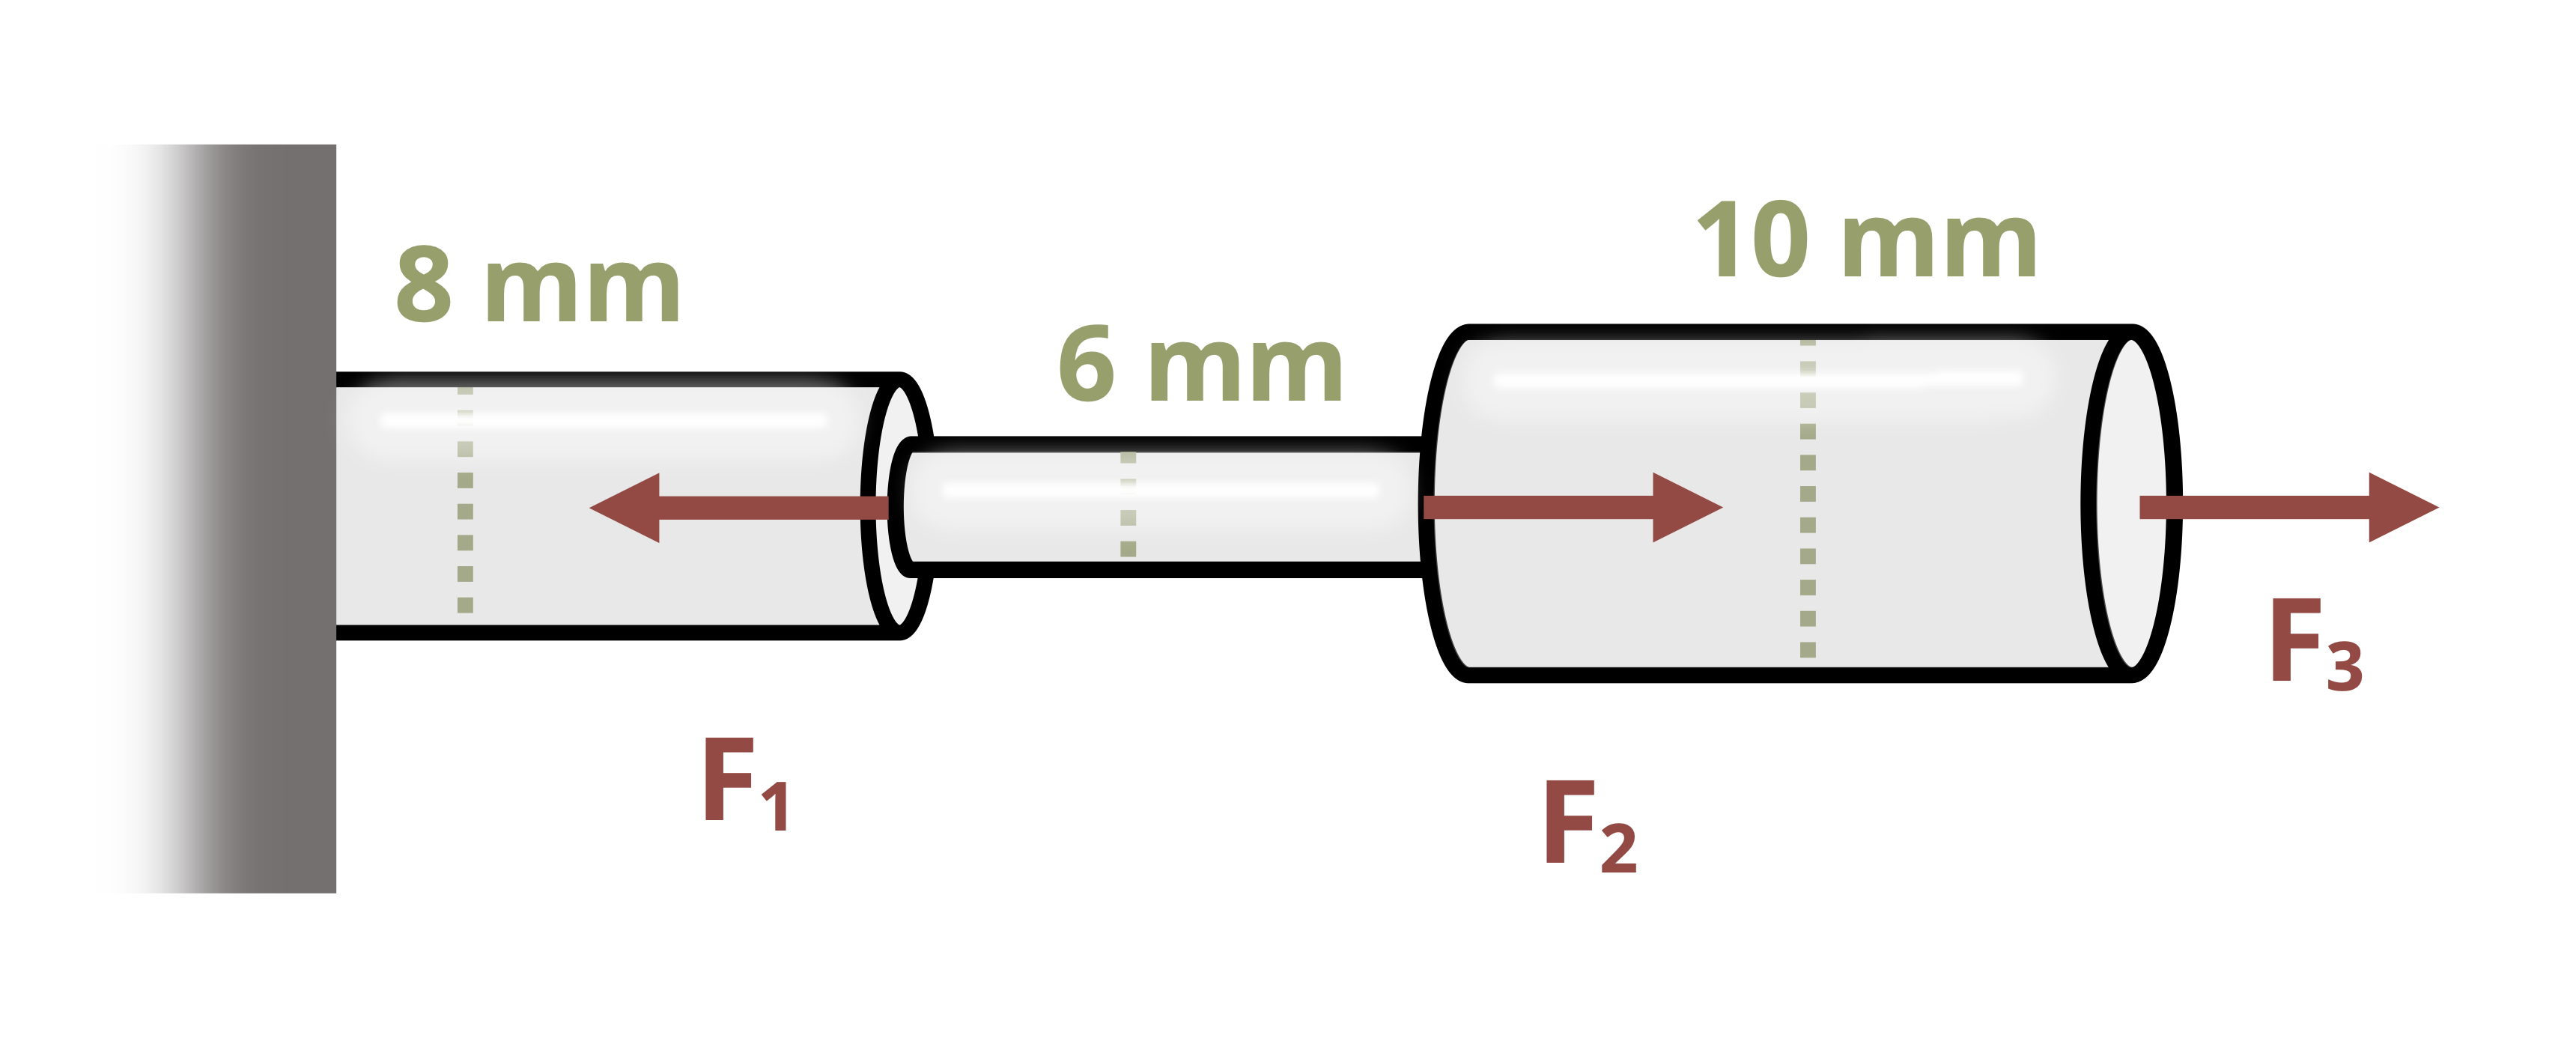
\includegraphics{images/138.png}

}

\caption{Figure 1: A series of solid circular bars are loaded with three
loads}

\end{figure}%

\begin{Shaded}
\begin{Highlighting}[]
\NormalTok{\#| standalone: true}
\NormalTok{\#| viewerHeight: 600}
\NormalTok{\#| components: [viewer]}

\NormalTok{from shiny import App, render, ui, reactive}
\NormalTok{import random}
\NormalTok{import asyncio}
\NormalTok{import io}
\NormalTok{import math}
\NormalTok{import string}
\NormalTok{from datetime import datetime}
\NormalTok{from pathlib import Path}


\NormalTok{def generate\_random\_letters(length):}
\NormalTok{    \# Generate a random string of letters of specified length}
\NormalTok{    return \textquotesingle{}\textquotesingle{}.join(random.choice(string.ascii\_lowercase) for \_ in range(length))  }

\NormalTok{problem\_ID="138"}
\NormalTok{F1=reactive.Value("\_\_")}
\NormalTok{F2=reactive.Value("\_\_")}
\NormalTok{F3=reactive.Value("\_\_")}
\NormalTok{d1=8}
\NormalTok{d2=6}
\NormalTok{d3=10}
\NormalTok{attempts=["Timestamp,Attempt,Answer,Feedback\textbackslash{}n"]}

\NormalTok{app\_ui = ui.page\_fluid(}
\NormalTok{    ui.markdown("**Please enter your ID number from your instructor and click to generate your problem**"),}
\NormalTok{    ui.input\_text("ID","", placeholder="Enter ID Number Here"),}
\NormalTok{    ui.input\_action\_button("generate\_problem", "Generate Problem", class\_="btn{-}primary"),}
\NormalTok{    ui.markdown("**Problem Statement**"),}
\NormalTok{    ui.output\_ui("ui\_problem\_statement"),}
\NormalTok{    ui.input\_text("answer","Your Answer in units of MPa", placeholder="Please enter your answer"),}
\NormalTok{    ui.input\_action\_button("submit", "Submit Answer", class\_="btn{-}primary"),}
\NormalTok{    ui.download\_button("download", "Download File to Submit", class\_="btn{-}success"),}
\NormalTok{)}


\NormalTok{def server(input, output, session):}
\NormalTok{    \# Initialize a counter for attempts}
\NormalTok{    attempt\_counter = reactive.Value(0)}
    
\NormalTok{    @output}
\NormalTok{    @render.ui}
\NormalTok{    def ui\_problem\_statement():}
\NormalTok{        return[ui.markdown(f"A series of solid circular bars are loaded with three loads as shown, F\textless{}sub\textgreater{}1\textless{}/sub\textgreater{} = \{F1()\} N, F\textless{}sub\textgreater{}2\textless{}/sub\textgreater{} = \{F2()\} N, and F\textless{}sub\textgreater{}3\textless{}/sub\textgreater{} = \{F3()\} N. What is the largest absolute normal stress in any bar?")]}
     
\NormalTok{    @reactive.Effect}
\NormalTok{    @reactive.event(input.generate\_problem)}
\NormalTok{    def randomize\_vars():}
\NormalTok{        random.seed(input.ID())}
\NormalTok{        F1.set(random.randrange(50, 70, 1))}
\NormalTok{        F2.set(random.randrange(10, 30, 1))}
\NormalTok{        F3.set(F1(){-}F2())}
        

\NormalTok{    @reactive.Effect}
\NormalTok{    @reactive.event(input.submit)}
\NormalTok{    def \_():}
\NormalTok{        attempt\_counter.set(attempt\_counter() + 1)  \# Increment the attempt counter on each submission.}
        
\NormalTok{        \# Calculate the instructor\textquotesingle{}s answer and determine if the user\textquotesingle{}s answer is correct.}
\NormalTok{        instr= (F1()/(math.pi*(d2/(1000*2))**2))/10**6}
        
\NormalTok{        if math.isclose(float(input.answer()), instr, rel\_tol=0.01):}
\NormalTok{            check = "*Correct*"}
\NormalTok{            correct\_indicator = "JL"}
\NormalTok{        else:}
\NormalTok{            check = "*Not Correct.*"}
\NormalTok{            correct\_indicator = "JG"}

\NormalTok{        \# Generate random parts for the encoded attempt.}
\NormalTok{        random\_start = generate\_random\_letters(4)}
\NormalTok{        random\_middle = generate\_random\_letters(4)}
\NormalTok{        random\_end = generate\_random\_letters(4)}
\NormalTok{        encoded\_attempt = f"\{random\_start\}\{problem\_ID\}{-}\{random\_middle\}\{attempt\_counter()\}\{correct\_indicator\}{-}\{random\_end\}\{input.ID()\}"}

\NormalTok{        \# Store the most recent encoded attempt in a reactive value so it persists across submissions}
\NormalTok{        session.encoded\_attempt = reactive.Value(encoded\_attempt)}

\NormalTok{        \# Append the attempt data to the attempts list without the encoded attempt}
\NormalTok{        attempts.append(f"\{datetime.now()\}, \{attempt\_counter()\}, \{input.answer()\}, \{check\}\textbackslash{}n")}

\NormalTok{        \# Show feedback to the user.}
\NormalTok{        feedback = ui.markdown(f"Your answer of \{input.answer()\} is \{check\}.")}
\NormalTok{        m = ui.modal(}
\NormalTok{            feedback,}
\NormalTok{            title="Feedback",}
\NormalTok{            easy\_close=True}
\NormalTok{        )}
\NormalTok{        ui.modal\_show(m)}

\NormalTok{    @session.download(filename=lambda: f"Problem\_Log{-}\{problem\_ID\}{-}\{input.ID()\}.csv")}
\NormalTok{    async def download():}
\NormalTok{        \# Start the CSV with the encoded attempt (without label)}
\NormalTok{        final\_encoded = session.encoded\_attempt() if session.encoded\_attempt is not None else "No attempts"}
\NormalTok{        yield f"\{final\_encoded\}\textbackslash{}n\textbackslash{}n"}
        
\NormalTok{        \# Write the header for the remaining CSV data once}
\NormalTok{        yield "Timestamp,Attempt,Answer,Feedback\textbackslash{}n"}
        
\NormalTok{        \# Write the attempts data, ensure that the header from the attempts list is not written again}
\NormalTok{        for attempt in attempts[1:]:  \# Skip the first element which is the header}
\NormalTok{            await asyncio.sleep(0.25)  \# This delay may not be necessary; adjust as needed}
\NormalTok{            yield attempt}


\NormalTok{\# App installation}
\NormalTok{app = App(app\_ui, server)}
\end{Highlighting}
\end{Shaded}

\chapter*{Problem 2.2}\label{problem-2.2-2}
\addcontentsline{toc}{chapter}{Problem 2.2}

\markboth{Problem 2.2}{Problem 2.2}

This is a dynamic rendering of the problem with dynamic variables based
on the username entered.

\section*{Problem Image}\label{problem-image-21}
\addcontentsline{toc}{section}{Problem Image}

\markright{Problem Image}

\begin{figure}[H]

{\centering 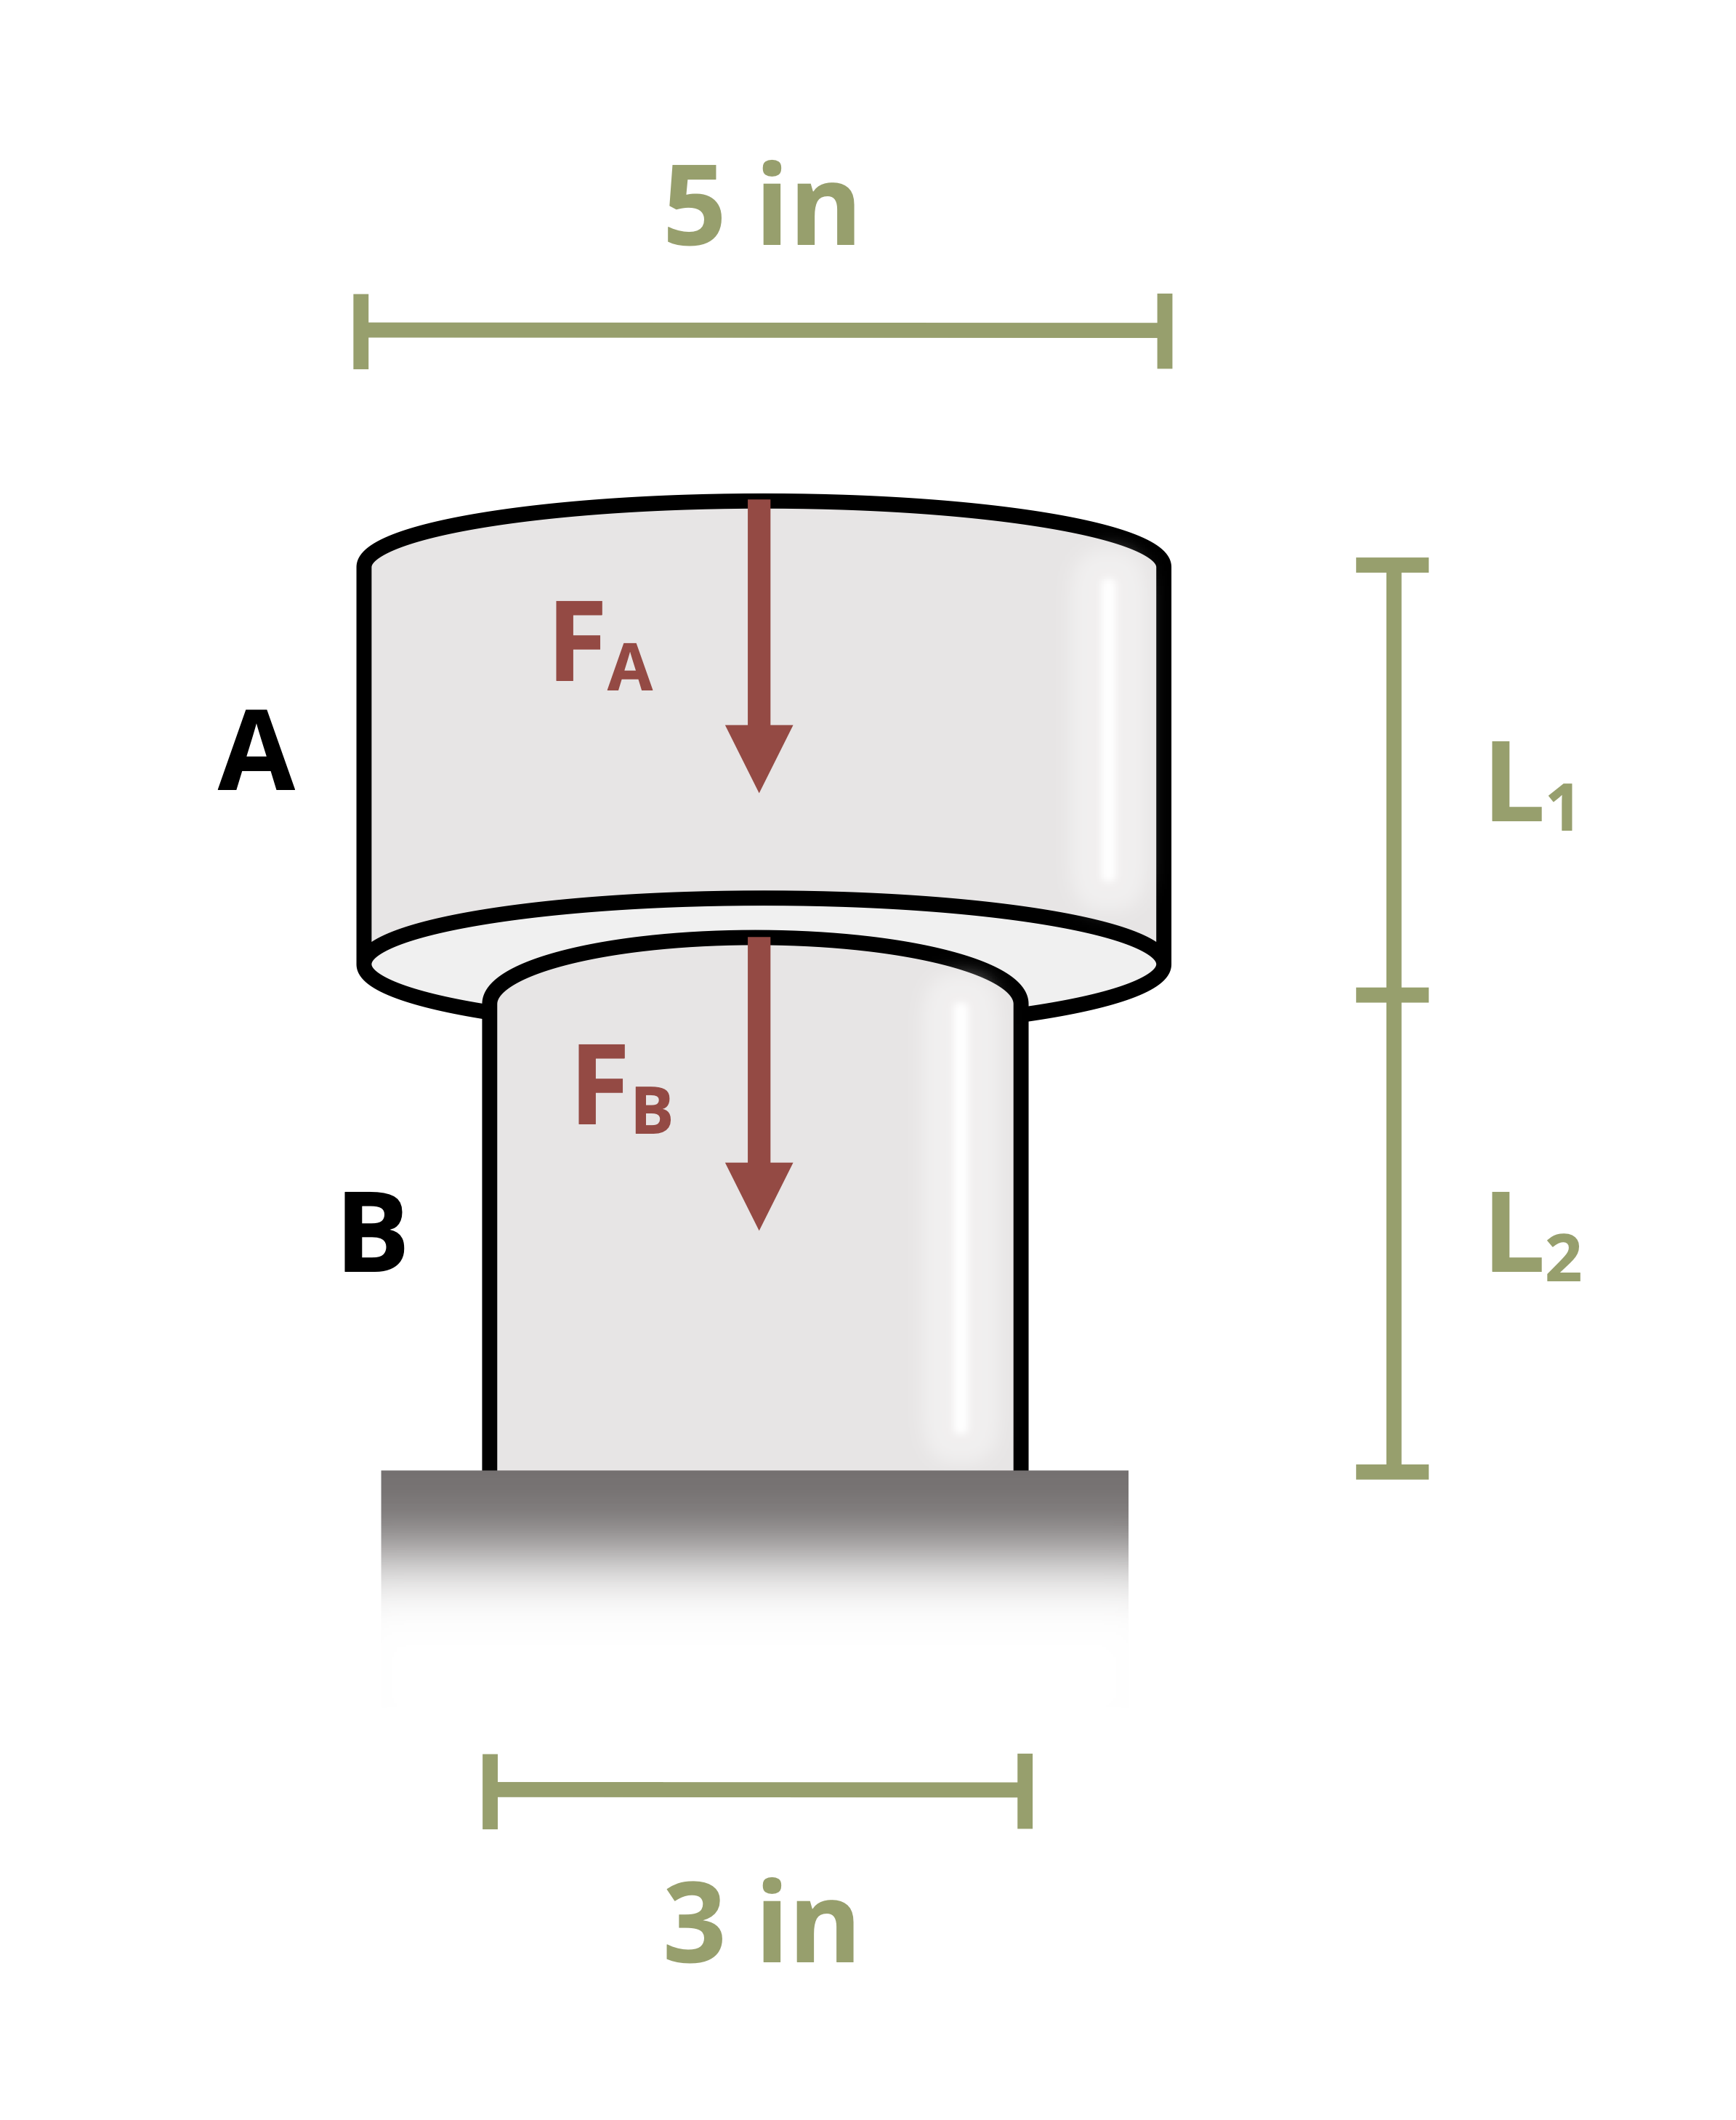
\includegraphics{images/139.png}

}

\caption{Figure 1: Two cylinders are stacked on top of each other.}

\end{figure}%

\begin{Shaded}
\begin{Highlighting}[]
\NormalTok{\#| standalone: true}
\NormalTok{\#| viewerHeight: 600}
\NormalTok{\#| components: [viewer]}

\NormalTok{from shiny import App, render, ui, reactive}
\NormalTok{import random}
\NormalTok{import asyncio}
\NormalTok{import io}
\NormalTok{import math}
\NormalTok{import string}
\NormalTok{from datetime import datetime}
\NormalTok{from pathlib import Path}

\NormalTok{def generate\_random\_letters(length):}
\NormalTok{    \# Generate a random string of letters of specified length}
\NormalTok{    return \textquotesingle{}\textquotesingle{}.join(random.choice(string.ascii\_lowercase) for \_ in range(length))  }

\NormalTok{problem\_ID="139"}
\NormalTok{L1=reactive.Value("\_\_")}
\NormalTok{L2=reactive.Value("\_\_")}
\NormalTok{FA=reactive.Value("\_\_")}
\NormalTok{FB=reactive.Value("\_\_")}
\NormalTok{E = 30*10**6}
  
\NormalTok{attempts=["Timestamp,Attempt,Answer,Feedback\textbackslash{}n"]}

\NormalTok{app\_ui = ui.page\_fluid(}
\NormalTok{    ui.markdown("**Please enter your ID number from your instructor and click to generate your problem**"),}
\NormalTok{    ui.input\_text("ID","", placeholder="Enter ID Number Here"),}
\NormalTok{    ui.input\_action\_button("generate\_problem", "Generate Problem", class\_="btn{-}primary"),}
\NormalTok{    ui.markdown("**Problem Statement**"),}
\NormalTok{    ui.output\_ui("ui\_problem\_statement"),}
\NormalTok{    ui.input\_text("answer","Your Answer in units of inches", placeholder="Please enter your answer"),}
\NormalTok{    ui.input\_action\_button("submit", "Submit Answer", class\_="btn{-}primary"),}
\NormalTok{    ui.download\_button("download", "Download File to Submit", class\_="btn{-}success"),}
\NormalTok{)}

\NormalTok{def server(input, output, session):}
\NormalTok{    \# Initialize a counter for attempts}
\NormalTok{    attempt\_counter = reactive.Value(0)}

\NormalTok{    @output}
\NormalTok{    @render.ui}
\NormalTok{    def ui\_problem\_statement():}
\NormalTok{        return[ui.markdown(f"Two cylinders are stacked on top of one another and two forces are applied at the top surface and at the joint between the cylinders as shown. If L\textless{}sub\textgreater{}1\textless{}/sub\textgreater{} = \{L1()\} in., L\textless{}sub\textgreater{}2\textless{}/sub\textgreater{} = \{L2()\} in., F\textless{}sub\textgreater{}A\textless{}/sub\textgreater{} = \{FA()\} lb, and F\textless{}sub\textgreater{}B\textless{}/sub\textgreater{} = \{FB()\} lb, find the total deflection in the stack of cylinders. Assume E = 30 x 10\textless{}sup\textgreater{}6\textless{}/sup\textgreater{} psi for both cylinders. ")]}
    
\NormalTok{    @reactive.Effect}
\NormalTok{    @reactive.event(input.generate\_problem)}
\NormalTok{    def randomize\_vars():}
\NormalTok{        random.seed(input.ID())}
\NormalTok{        FA.set(random.randrange(300, 700, 10))}
\NormalTok{        FB.set(random.randrange(100, 300, 10))}
\NormalTok{        L1.set(random.randrange(2, 7, 1))}
\NormalTok{        L2.set(L1() * 1.3)}
        
\NormalTok{    @reactive.Effect}
\NormalTok{    @reactive.event(input.submit)}
\NormalTok{    def \_():}
\NormalTok{        attempt\_counter.set(attempt\_counter() + 1)  \# Increment the attempt counter on each submission.}
    
\NormalTok{        instr= (FA()*L1())/((math.pi*(5/2)**2)*E) + ((FB()+FA())*L2())/((math.pi*(3/2)**2)*E)}
\NormalTok{        if math.isclose(float(input.answer()), instr, rel\_tol=0.01):}
\NormalTok{            check = "*Correct*"}
\NormalTok{            correct\_indicator = "JL"}
\NormalTok{        else:}
\NormalTok{            check = "*Not Correct.*"}
\NormalTok{            correct\_indicator = "JG"}

\NormalTok{        \# Generate random parts for the encoded attempt.}
\NormalTok{        random\_start = generate\_random\_letters(4)}
\NormalTok{        random\_middle = generate\_random\_letters(4)}
\NormalTok{        random\_end = generate\_random\_letters(4)}
\NormalTok{        encoded\_attempt = f"\{random\_start\}\{problem\_ID\}{-}\{random\_middle\}\{attempt\_counter()\}\{correct\_indicator\}{-}\{random\_end\}\{input.ID()\}"}

\NormalTok{        \# Store the most recent encoded attempt in a reactive value so it persists across submissions}
\NormalTok{        session.encoded\_attempt = reactive.Value(encoded\_attempt)}

\NormalTok{        \# Append the attempt data to the attempts list without the encoded attempt}
\NormalTok{        attempts.append(f"\{datetime.now()\}, \{attempt\_counter()\}, \{input.answer()\}, \{check\}\textbackslash{}n")}

\NormalTok{        \# Show feedback to the user.}
\NormalTok{        feedback = ui.markdown(f"Your answer of \{input.answer()\} is \{check\}.")}
\NormalTok{        m = ui.modal(}
\NormalTok{            feedback,}
\NormalTok{            title="Feedback",}
\NormalTok{            easy\_close=True}
\NormalTok{        )}
\NormalTok{        ui.modal\_show(m)}

\NormalTok{    @session.download(filename=lambda: f"Problem\_Log{-}\{problem\_ID\}{-}\{input.ID()\}.csv")}
\NormalTok{    async def download():}
\NormalTok{        \# Start the CSV with the encoded attempt (without label)}
\NormalTok{        final\_encoded = session.encoded\_attempt() if session.encoded\_attempt is not None else "No attempts"}
\NormalTok{        yield f"\{final\_encoded\}\textbackslash{}n\textbackslash{}n"}
        
\NormalTok{        \# Write the header for the remaining CSV data once}
\NormalTok{        yield "Timestamp,Attempt,Answer,Feedback\textbackslash{}n"}
        
\NormalTok{        \# Write the attempts data, ensure that the header from the attempts list is not written again}
\NormalTok{        for attempt in attempts[1:]:  \# Skip the first element which is the header}
\NormalTok{            await asyncio.sleep(0.25)  \# This delay may not be necessary; adjust as needed}
\NormalTok{            yield attempt}

\NormalTok{\# App installation}
\NormalTok{app = App(app\_ui, server)}
\end{Highlighting}
\end{Shaded}

\chapter*{Problem 2.3}\label{problem-2.3-2}
\addcontentsline{toc}{chapter}{Problem 2.3}

\markboth{Problem 2.3}{Problem 2.3}

This is a dynamic rendering of the problem with dynamic variables based
on the username entered.

\section*{Problem Image}\label{problem-image-22}
\addcontentsline{toc}{section}{Problem Image}

\markright{Problem Image}

\begin{figure}[H]

{\centering 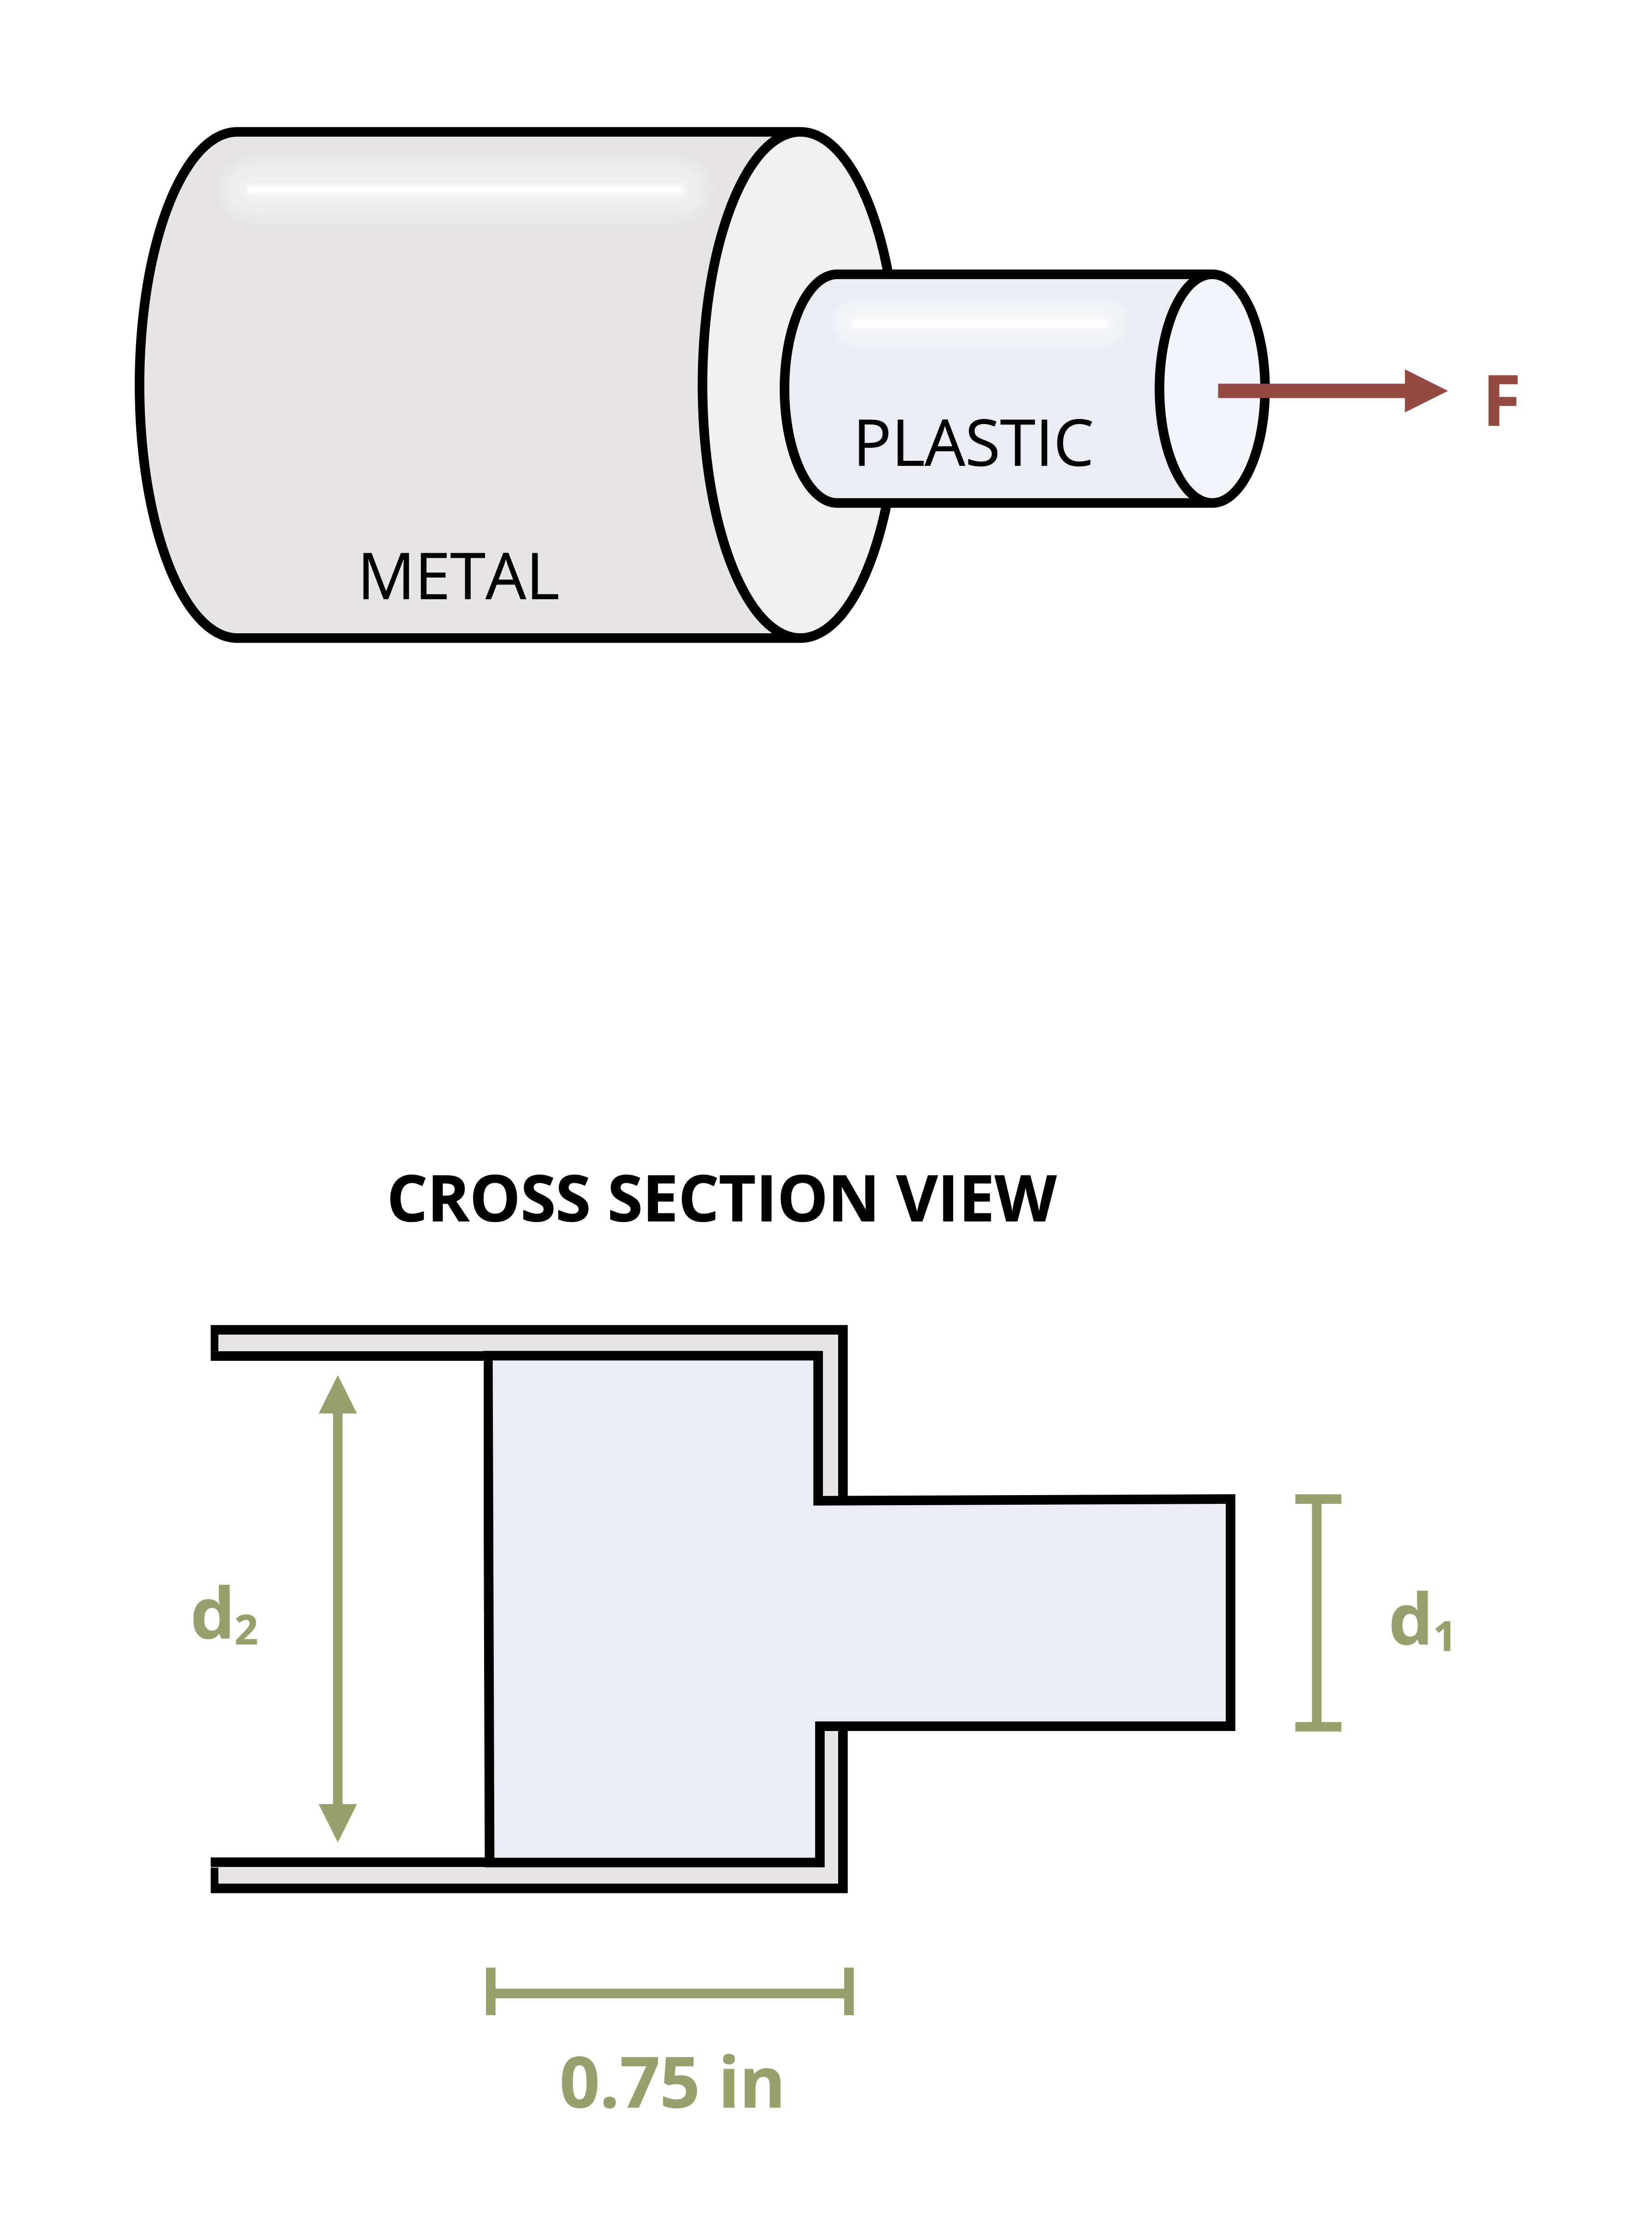
\includegraphics{images/144.png}

}

\caption{Figure 1: A plastic cylindrical peg is constrained by a metal
cap}

\end{figure}%

\begin{Shaded}
\begin{Highlighting}[]
\NormalTok{\#| standalone: true}
\NormalTok{\#| viewerHeight: 600}
\NormalTok{\#| components: [viewer]}

\NormalTok{from shiny import App, render, ui, reactive}
\NormalTok{import random}
\NormalTok{import asyncio}
\NormalTok{import io}
\NormalTok{import math}
\NormalTok{import string}
\NormalTok{from datetime import datetime}
\NormalTok{from pathlib import Path}

\NormalTok{def generate\_random\_letters(length):}
\NormalTok{    \# Generate a random string of letters of specified length}
\NormalTok{    return \textquotesingle{}\textquotesingle{}.join(random.choice(string.ascii\_lowercase) for \_ in range(length))}

\NormalTok{problem\_ID="144"}
\NormalTok{F=reactive.Value("\_\_")}
\NormalTok{d1=reactive.Value("\_\_")}
\NormalTok{d2=reactive.Value("\_\_")}

\NormalTok{attempts=["Timestamp,Attempt,Answer,Feedback\textbackslash{}n"]}

\NormalTok{app\_ui = ui.page\_fluid(}
\NormalTok{    ui.markdown("**Please enter your ID number from your instructor and click to generate your problem**"),}
\NormalTok{    ui.input\_text("ID","", placeholder="Enter ID Number Here"),}
\NormalTok{    ui.input\_action\_button("generate\_problem", "Generate Problem", class\_="btn{-}primary"),}
\NormalTok{    ui.markdown("**Problem Statement**"),}
\NormalTok{    ui.output\_ui("ui\_problem\_statement"),}
\NormalTok{    ui.input\_text("answer","Your Answer in units of psi", placeholder="Please enter your answer"),}
\NormalTok{    ui.input\_action\_button("submit", "Submit Answer", class\_="btn{-}primary"),}
\NormalTok{    ui.download\_button("download", "Download File to Submit", class\_="btn{-}success"),}
\NormalTok{)}


\NormalTok{def server(input, output, session):}
\NormalTok{    \# Initialize a counter for attempts}
\NormalTok{    attempt\_counter = reactive.Value(0)}

\NormalTok{    @output}
\NormalTok{    @render.ui}
\NormalTok{    def ui\_problem\_statement():}
\NormalTok{        return[ui.markdown(f"A plastic cylindrical peg is constrained by a metal cap as shown. An axial load of F = \{F()\} lb is applied to the peg. If d\textless{}sub\textgreater{}1\textless{}/sub\textgreater{} = \{d1()\} in and d\textless{}sub\textgreater{}2\textless{}/sub\textgreater{} = \{d2()\} in, determine the largest normal stress in the peg. Assume the axial load is evenly distributed across the peg and that the metal cap is fixed and does not move.")]}
    
\NormalTok{    @reactive.Effect}
\NormalTok{    @reactive.event(input.generate\_problem)}
\NormalTok{    def randomize\_vars():}
\NormalTok{        random.seed(input.ID())}
\NormalTok{        F.set(random.randrange(20, 80, 5))}
\NormalTok{        d1.set(random.randrange(3, 8, 1)/10)}
\NormalTok{        d2.set(round(d1() * 1.6, 2))}
        
 
\NormalTok{    @reactive.Effect}
\NormalTok{    @reactive.event(input.submit)}
\NormalTok{    def \_():}
\NormalTok{        attempt\_counter.set(attempt\_counter() + 1)  \# Increment the attempt counter on each submission.}
\NormalTok{        instr= F()/(math.pi*((d1()/2)**2))}
\NormalTok{        \#check=math.isclose(float(input.answer()),instr,rel\_tol=0.001)}
        
\NormalTok{        if math.isclose(float(input.answer()), instr, rel\_tol=0.01):}
\NormalTok{            check = "*Correct*"}
\NormalTok{            correct\_indicator = "JL"}
\NormalTok{        else:}
\NormalTok{            check = "*Not Correct.*"}
\NormalTok{            correct\_indicator = "JG"}

\NormalTok{        \# Generate random parts for the encoded attempt.}
\NormalTok{        random\_start = generate\_random\_letters(4)}
\NormalTok{        random\_middle = generate\_random\_letters(4)}
\NormalTok{        random\_end = generate\_random\_letters(4)}
\NormalTok{        encoded\_attempt = f"\{random\_start\}\{problem\_ID\}{-}\{random\_middle\}\{attempt\_counter()\}\{correct\_indicator\}{-}\{random\_end\}\{input.ID()\}"}

\NormalTok{        \# Store the most recent encoded attempt in a reactive value so it persists across submissions}
\NormalTok{        session.encoded\_attempt = reactive.Value(encoded\_attempt)}

\NormalTok{        \# Append the attempt data to the attempts list without the encoded attempt}
\NormalTok{        attempts.append(f"\{datetime.now()\}, \{attempt\_counter()\}, \{input.answer()\}, \{check\}\textbackslash{}n")}

\NormalTok{        \# Show feedback to the user.}
\NormalTok{        feedback = ui.markdown(f"Your answer of \{input.answer()\} is \{check\}.")}
\NormalTok{        m = ui.modal(}
\NormalTok{            feedback,}
\NormalTok{            title="Feedback",}
\NormalTok{            easy\_close=True}
\NormalTok{        )}
\NormalTok{        ui.modal\_show(m)}

\NormalTok{    @session.download(filename=lambda: f"Problem\_Log{-}\{problem\_ID\}{-}\{input.ID()\}.csv")}
\NormalTok{    async def download():}
\NormalTok{        \# Start the CSV with the encoded attempt (without label)}
\NormalTok{        final\_encoded = session.encoded\_attempt() if session.encoded\_attempt is not None else "No attempts"}
\NormalTok{        yield f"\{final\_encoded\}\textbackslash{}n\textbackslash{}n"}
        
\NormalTok{        \# Write the header for the remaining CSV data once}
\NormalTok{        yield "Timestamp,Attempt,Answer,Feedback\textbackslash{}n"}
        
\NormalTok{        \# Write the attempts data, ensure that the header from the attempts list is not written again}
\NormalTok{        for attempt in attempts[1:]:  \# Skip the first element which is the header}
\NormalTok{            await asyncio.sleep(0.25)  \# This delay may not be necessary; adjust as needed}
\NormalTok{            yield attempt}


\NormalTok{\# App installation}
\NormalTok{app = App(app\_ui, server)}
\end{Highlighting}
\end{Shaded}

\chapter*{Problem 2.4}\label{problem-2.4-2}
\addcontentsline{toc}{chapter}{Problem 2.4}

\markboth{Problem 2.4}{Problem 2.4}

This is a dynamic rendering of the problem with dynamic variables based
on the username entered.

\section*{Problem Image}\label{problem-image-23}
\addcontentsline{toc}{section}{Problem Image}

\markright{Problem Image}

\begin{figure}[H]

{\centering 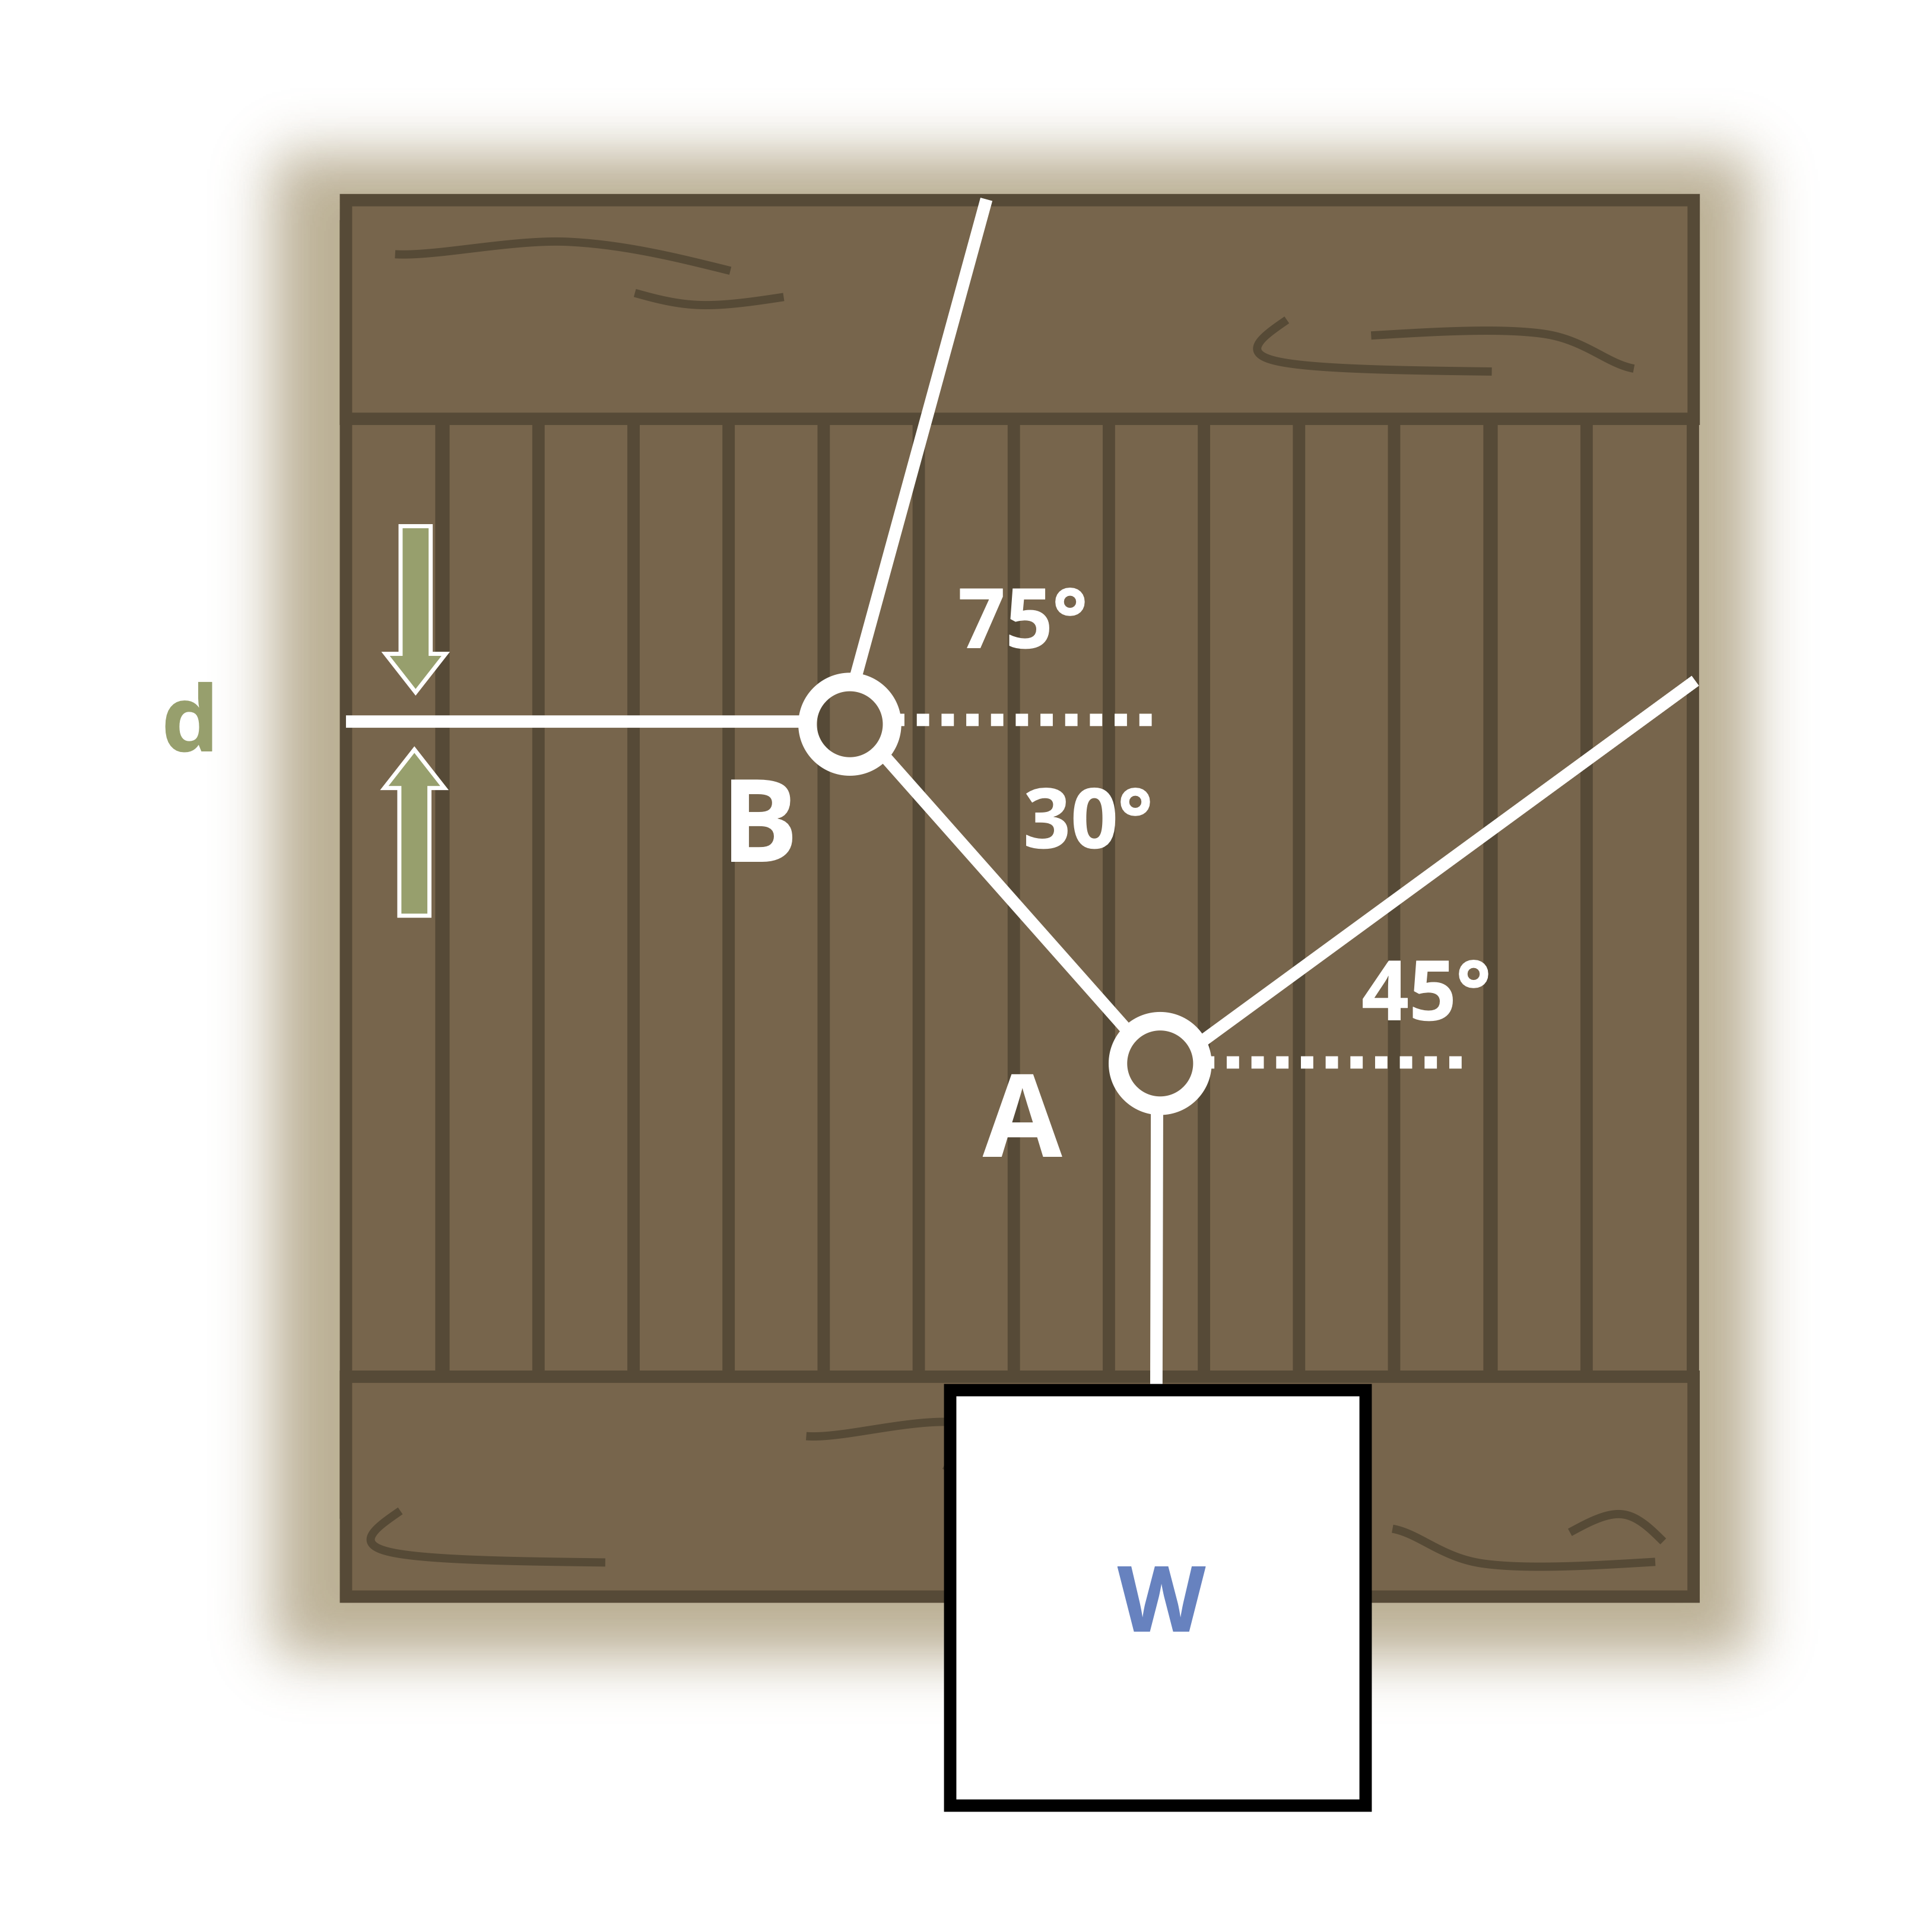
\includegraphics{images/146.png}

}

\caption{Figure 1: A crate is suspended by a set of cables.}

\end{figure}%

\begin{Shaded}
\begin{Highlighting}[]
\NormalTok{\#| standalone: true}
\NormalTok{\#| viewerHeight: 600}
\NormalTok{\#| components: [viewer]}

\NormalTok{from shiny import App, render, ui, reactive}
\NormalTok{import random}
\NormalTok{import asyncio}
\NormalTok{import io}
\NormalTok{import math}
\NormalTok{import string}
\NormalTok{from datetime import datetime}
\NormalTok{from pathlib import Path}


\NormalTok{def generate\_random\_letters(length):}
\NormalTok{    \# Generate a random string of letters of specified length}
\NormalTok{    return \textquotesingle{}\textquotesingle{}.join(random.choice(string.ascii\_lowercase) for \_ in range(length)) }

\NormalTok{problem\_ID="146"}
\NormalTok{W=reactive.Value("\_\_")}
\NormalTok{d=reactive.Value("\_\_")}
\NormalTok{angle1=math.radians(45)}
\NormalTok{angle2=math.radians(30)}
\NormalTok{angle3=math.radians(75)}

\NormalTok{attempts=["Timestamp,Attempt,Answer,Feedback\textbackslash{}n"]}

\NormalTok{app\_ui = ui.page\_fluid(}
\NormalTok{    ui.markdown("**Please enter your ID number from your instructor and click to generate your problem**"),}
\NormalTok{    ui.input\_text("ID","", placeholder="Enter ID Number Here"),}
\NormalTok{    ui.input\_action\_button("generate\_problem", "Generate Problem", class\_="btn{-}primary"),}
\NormalTok{    ui.markdown("**Problem Statement**"),}
\NormalTok{    ui.output\_ui("ui\_problem\_statement"),}
\NormalTok{    ui.input\_text("answer","Your Answer in units of GPa", placeholder="Please enter your answer"),}
\NormalTok{    ui.input\_action\_button("submit", "Submit Answer", class\_="btn{-}primary"),}
\NormalTok{    ui.download\_button("download", "Download File to Submit", class\_="btn{-}success"),}
\NormalTok{)}


\NormalTok{def server(input, output, session):}
\NormalTok{    \# Initialize a counter for attempts}
\NormalTok{    attempt\_counter = reactive.Value(0)}

\NormalTok{    @output}
\NormalTok{    @render.ui}
\NormalTok{    def ui\_problem\_statement():}
\NormalTok{        return[ui.markdown(f"A crate weighing \{W()\} kN is suspended by a set of cables. The diameter of each cable is \{d()\}  mm. What is the maximum stress in any cable, exluding the cable attached to the crate.")]}
    
\NormalTok{    @reactive.Effect}
\NormalTok{    @reactive.event(input.generate\_problem)}
\NormalTok{    def randomize\_vars():}
\NormalTok{        random.seed(input.ID())}
\NormalTok{        W.set(random.randrange(30, 90, 1))}
\NormalTok{        d.set(random.randrange(20, 90, 1)/10)}
        

\NormalTok{    @reactive.Effect}
\NormalTok{    @reactive.event(input.submit)}
\NormalTok{    def \_():}
\NormalTok{        attempt\_counter.set(attempt\_counter() + 1)  \# Increment the attempt counter on each submission.}
    
\NormalTok{        R1 = W()/(((math.cos(angle1)/math.cos(angle2))*math.sin(angle2))+math.sin(angle1))}
\NormalTok{        instr= (R1*10**3/(math.pi*((d()/(1000*2))**2)))/10**9}
\NormalTok{        if math.isclose(float(input.answer()), instr, rel\_tol=0.01):}
\NormalTok{            check = "*Correct*"}
\NormalTok{            correct\_indicator = "JL"}
\NormalTok{        else:}
\NormalTok{            check = "*Not Correct.*"}
\NormalTok{            correct\_indicator = "JG"}

\NormalTok{        \# Generate random parts for the encoded attempt.}
\NormalTok{        random\_start = generate\_random\_letters(4)}
\NormalTok{        random\_middle = generate\_random\_letters(4)}
\NormalTok{        random\_end = generate\_random\_letters(4)}
\NormalTok{        encoded\_attempt = f"\{random\_start\}\{problem\_ID\}{-}\{random\_middle\}\{attempt\_counter()\}\{correct\_indicator\}{-}\{random\_end\}\{input.ID()\}"}

\NormalTok{        \# Store the most recent encoded attempt in a reactive value so it persists across submissions}
\NormalTok{        session.encoded\_attempt = reactive.Value(encoded\_attempt)}

\NormalTok{        \# Append the attempt data to the attempts list without the encoded attempt}
\NormalTok{        attempts.append(f"\{datetime.now()\}, \{attempt\_counter()\}, \{input.answer()\}, \{check\}\textbackslash{}n")}

\NormalTok{        \# Show feedback to the user.}
\NormalTok{        feedback = ui.markdown(f"Your answer of \{input.answer()\} is \{check\}.")}
\NormalTok{        m = ui.modal(}
\NormalTok{            feedback,}
\NormalTok{            title="Feedback",}
\NormalTok{            easy\_close=True}
\NormalTok{        )}
\NormalTok{        ui.modal\_show(m)}

\NormalTok{    @session.download(filename=lambda: f"Problem\_Log{-}\{problem\_ID\}{-}\{input.ID()\}.csv")}
\NormalTok{    async def download():}
\NormalTok{        \# Start the CSV with the encoded attempt (without label)}
\NormalTok{        final\_encoded = session.encoded\_attempt() if session.encoded\_attempt is not None else "No attempts"}
\NormalTok{        yield f"\{final\_encoded\}\textbackslash{}n\textbackslash{}n"}
        
\NormalTok{        \# Write the header for the remaining CSV data once}
\NormalTok{        yield "Timestamp,Attempt,Answer,Feedback\textbackslash{}n"}
        
\NormalTok{        \# Write the attempts data, ensure that the header from the attempts list is not written again}
\NormalTok{        for attempt in attempts[1:]:  \# Skip the first element which is the header}
\NormalTok{            await asyncio.sleep(0.25)  \# This delay may not be necessary; adjust as needed}
\NormalTok{            yield attempt}


\NormalTok{\# App installation}
\NormalTok{app = App(app\_ui, server)}
\end{Highlighting}
\end{Shaded}

\chapter*{Problem 2.21}\label{problem-2.21-2}
\addcontentsline{toc}{chapter}{Problem 2.21}

\markboth{Problem 2.21}{Problem 2.21}

This is a dynamic rendering of the problem with dynamic variables based
on the username entered.

\section*{Problem Image}\label{problem-image-24}
\addcontentsline{toc}{section}{Problem Image}

\markright{Problem Image}

\begin{figure}[H]

{\centering 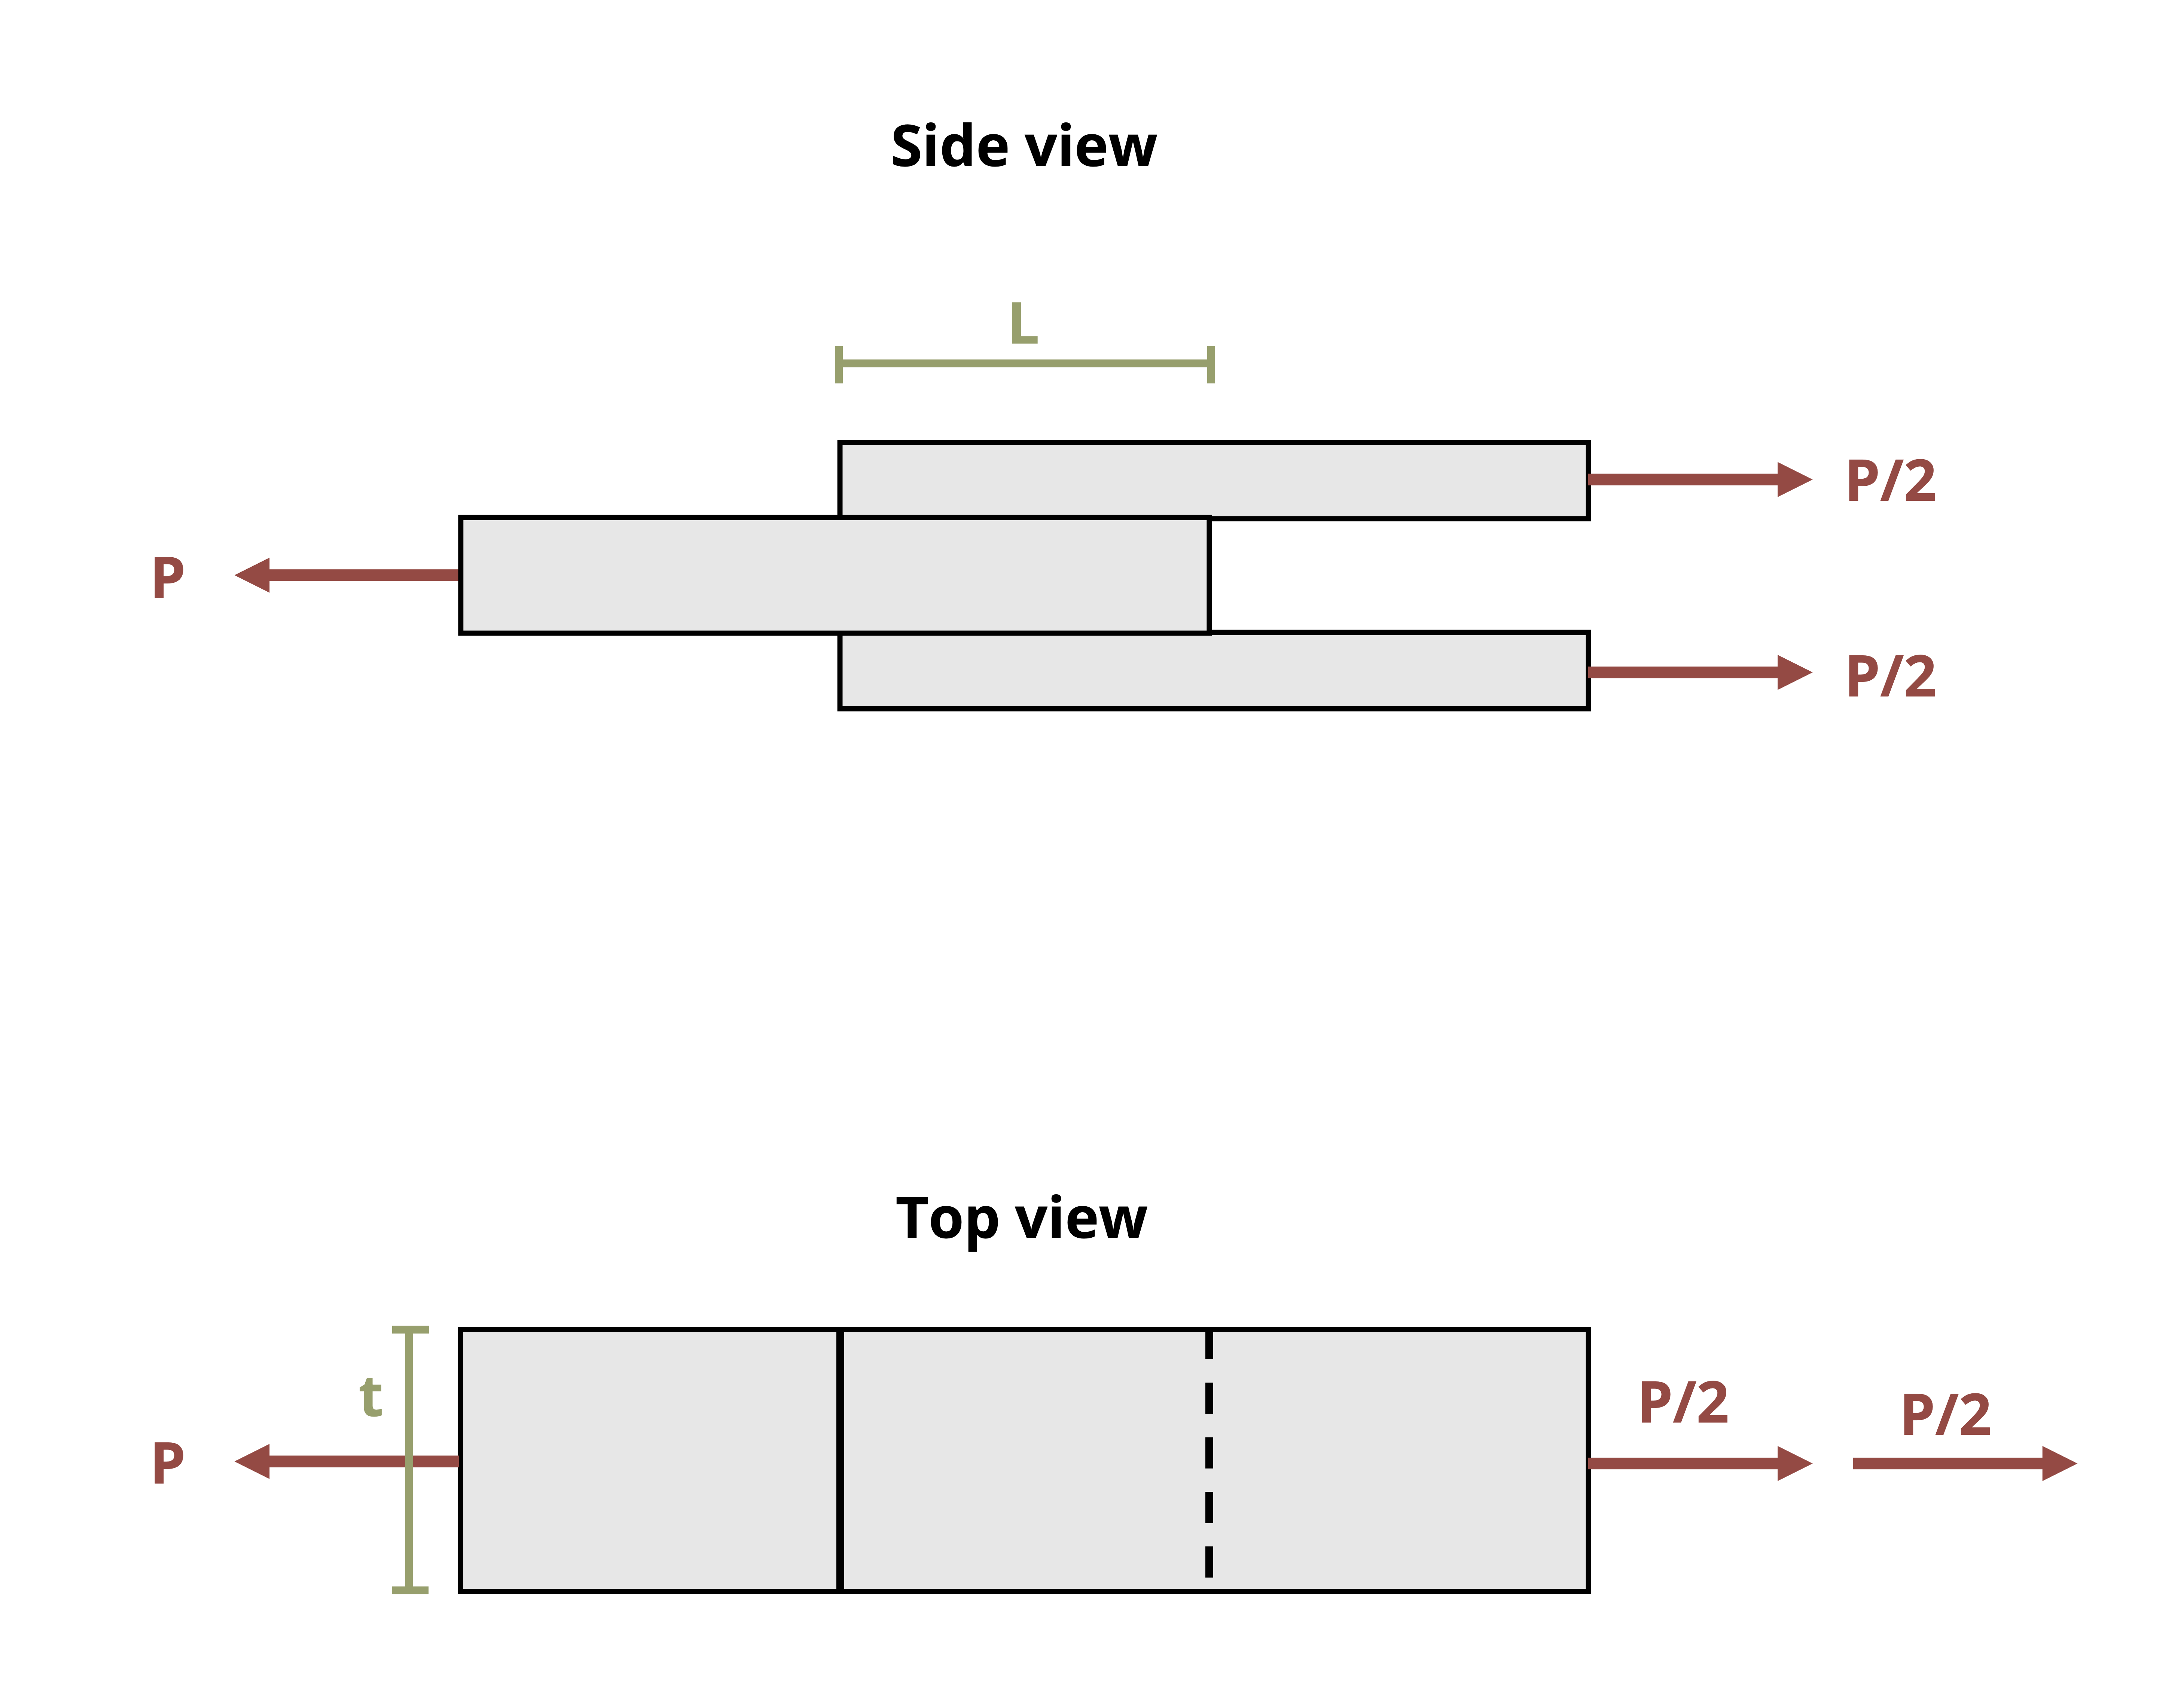
\includegraphics{images/164.png}

}

\caption{Figure 1: A double lap joint is glued together}

\end{figure}%

\begin{Shaded}
\begin{Highlighting}[]
\NormalTok{\#| standalone: true}
\NormalTok{\#| viewerHeight: 600}
\NormalTok{\#| components: [viewer]}

\NormalTok{from shiny import App, render, ui, reactive}
\NormalTok{import random}
\NormalTok{import asyncio}
\NormalTok{import io}
\NormalTok{import math}
\NormalTok{import string}
\NormalTok{from datetime import datetime}
\NormalTok{from pathlib import Path}

\NormalTok{def generate\_random\_letters(length):}
\NormalTok{    \# Generate a random string of letters of specified length}
\NormalTok{    return \textquotesingle{}\textquotesingle{}.join(random.choice(string.ascii\_lowercase) for \_ in range(length))  }

\NormalTok{problem\_ID="164"}
\NormalTok{τfail=reactive.Value("\_\_")}
\NormalTok{L=reactive.Value("\_\_")}
\NormalTok{t=reactive.Value("\_\_")}

\NormalTok{attempts=["Timestamp,Attempt,Answer,Feedback\textbackslash{}n"]}

\NormalTok{app\_ui = ui.page\_fluid(}
\NormalTok{    ui.markdown("**Please enter your ID number from your instructor and click to generate your problem**"),}
\NormalTok{    ui.input\_text("ID","", placeholder="Enter ID Number Here"),}
\NormalTok{    ui.input\_action\_button("generate\_problem", "Generate Problem", class\_="btn{-}primary"),}
\NormalTok{    ui.markdown("**Problem Statement**"),}
\NormalTok{    ui.output\_ui("ui\_problem\_statement"),}
\NormalTok{    ui.input\_text("answer","Your Answer in units of kips", placeholder="Please enter your answer"),}
\NormalTok{    ui.input\_action\_button("submit", "Submit Answer", class\_="btn{-}primary"),}
\NormalTok{    ui.download\_button("download", "Download File to Submit", class\_="btn{-}success"),}
\NormalTok{)}


\NormalTok{def server(input, output, session):}
\NormalTok{    \# Initialize a counter for attempts}
\NormalTok{    attempt\_counter = reactive.Value(0)}

\NormalTok{    @output}
\NormalTok{    @render.ui}
\NormalTok{    def ui\_problem\_statement():}
\NormalTok{        return[ui.markdown(f"A double lap joint is glued together using glue with a shear stress failure strength of \{τfail()\} psi. If dimensions L = \{L()\} in. and t = \{t()\} in., what is the maximum load P that the joint can withstand? Assume the load is evenly distributed across the joint on both sides.")]}
    
\NormalTok{    @reactive.Effect}
\NormalTok{    @reactive.event(input.generate\_problem)}
\NormalTok{    def randomize\_vars():}
\NormalTok{        random.seed(input.ID())}
\NormalTok{        τfail.set(random.randrange(7000, 9000, 100))}
\NormalTok{        L.set(random.randrange(40, 100, 1)/10)}
\NormalTok{        t.set(random.randrange(40, 100, 1)/10)}
        

\NormalTok{    @reactive.Effect}
\NormalTok{    @reactive.event(input.submit)}
\NormalTok{    def \_():}
\NormalTok{        attempt\_counter.set(attempt\_counter() + 1)  \# Increment the attempt counter on each submission.}
    
\NormalTok{        A = L()*t()*2}
\NormalTok{        instr= (τfail()*A)/1000}
\NormalTok{        if math.isclose(float(input.answer()), instr, rel\_tol=0.01):}
\NormalTok{            check = "*Correct*"}
\NormalTok{            correct\_indicator = "JL"}
\NormalTok{        else:}
\NormalTok{            check = "*Not Correct.*"}
\NormalTok{            correct\_indicator = "JG"}

\NormalTok{        \# Generate random parts for the encoded attempt.}
\NormalTok{        random\_start = generate\_random\_letters(4)}
\NormalTok{        random\_middle = generate\_random\_letters(4)}
\NormalTok{        random\_end = generate\_random\_letters(4)}
\NormalTok{        encoded\_attempt = f"\{random\_start\}\{problem\_ID\}{-}\{random\_middle\}\{attempt\_counter()\}\{correct\_indicator\}{-}\{random\_end\}\{input.ID()\}"}

\NormalTok{        \# Store the most recent encoded attempt in a reactive value so it persists across submissions}
\NormalTok{        session.encoded\_attempt = reactive.Value(encoded\_attempt)}

\NormalTok{        \# Append the attempt data to the attempts list without the encoded attempt}
\NormalTok{        attempts.append(f"\{datetime.now()\}, \{attempt\_counter()\}, \{input.answer()\}, \{check\}\textbackslash{}n")}

\NormalTok{        \# Show feedback to the user.}
\NormalTok{        feedback = ui.markdown(f"Your answer of \{input.answer()\} is \{check\}.")}
\NormalTok{        m = ui.modal(}
\NormalTok{            feedback,}
\NormalTok{            title="Feedback",}
\NormalTok{            easy\_close=True}
\NormalTok{        )}
\NormalTok{        ui.modal\_show(m)}

\NormalTok{    @session.download(filename=lambda: f"Problem\_Log{-}\{problem\_ID\}{-}\{input.ID()\}.csv")}
\NormalTok{    async def download():}
\NormalTok{        \# Start the CSV with the encoded attempt (without label)}
\NormalTok{        final\_encoded = session.encoded\_attempt() if session.encoded\_attempt is not None else "No attempts"}
\NormalTok{        yield f"\{final\_encoded\}\textbackslash{}n\textbackslash{}n"}
        
\NormalTok{        \# Write the header for the remaining CSV data once}
\NormalTok{        yield "Timestamp,Attempt,Answer,Feedback\textbackslash{}n"}
        
\NormalTok{        \# Write the attempts data, ensure that the header from the attempts list is not written again}
\NormalTok{        for attempt in attempts[1:]:  \# Skip the first element which is the header}
\NormalTok{            await asyncio.sleep(0.25)  \# This delay may not be necessary; adjust as needed}
\NormalTok{            yield attempt}


\NormalTok{\# App installation}
\NormalTok{app = App(app\_ui, server)}
\end{Highlighting}
\end{Shaded}

\chapter*{Problem 2.22}\label{problem-2.22-2}
\addcontentsline{toc}{chapter}{Problem 2.22}

\markboth{Problem 2.22}{Problem 2.22}

This is a dynamic rendering of the problem with dynamic variables based
on the username entered.

\section*{Problem Image}\label{problem-image-25}
\addcontentsline{toc}{section}{Problem Image}

\markright{Problem Image}

\begin{figure}[H]

{\centering 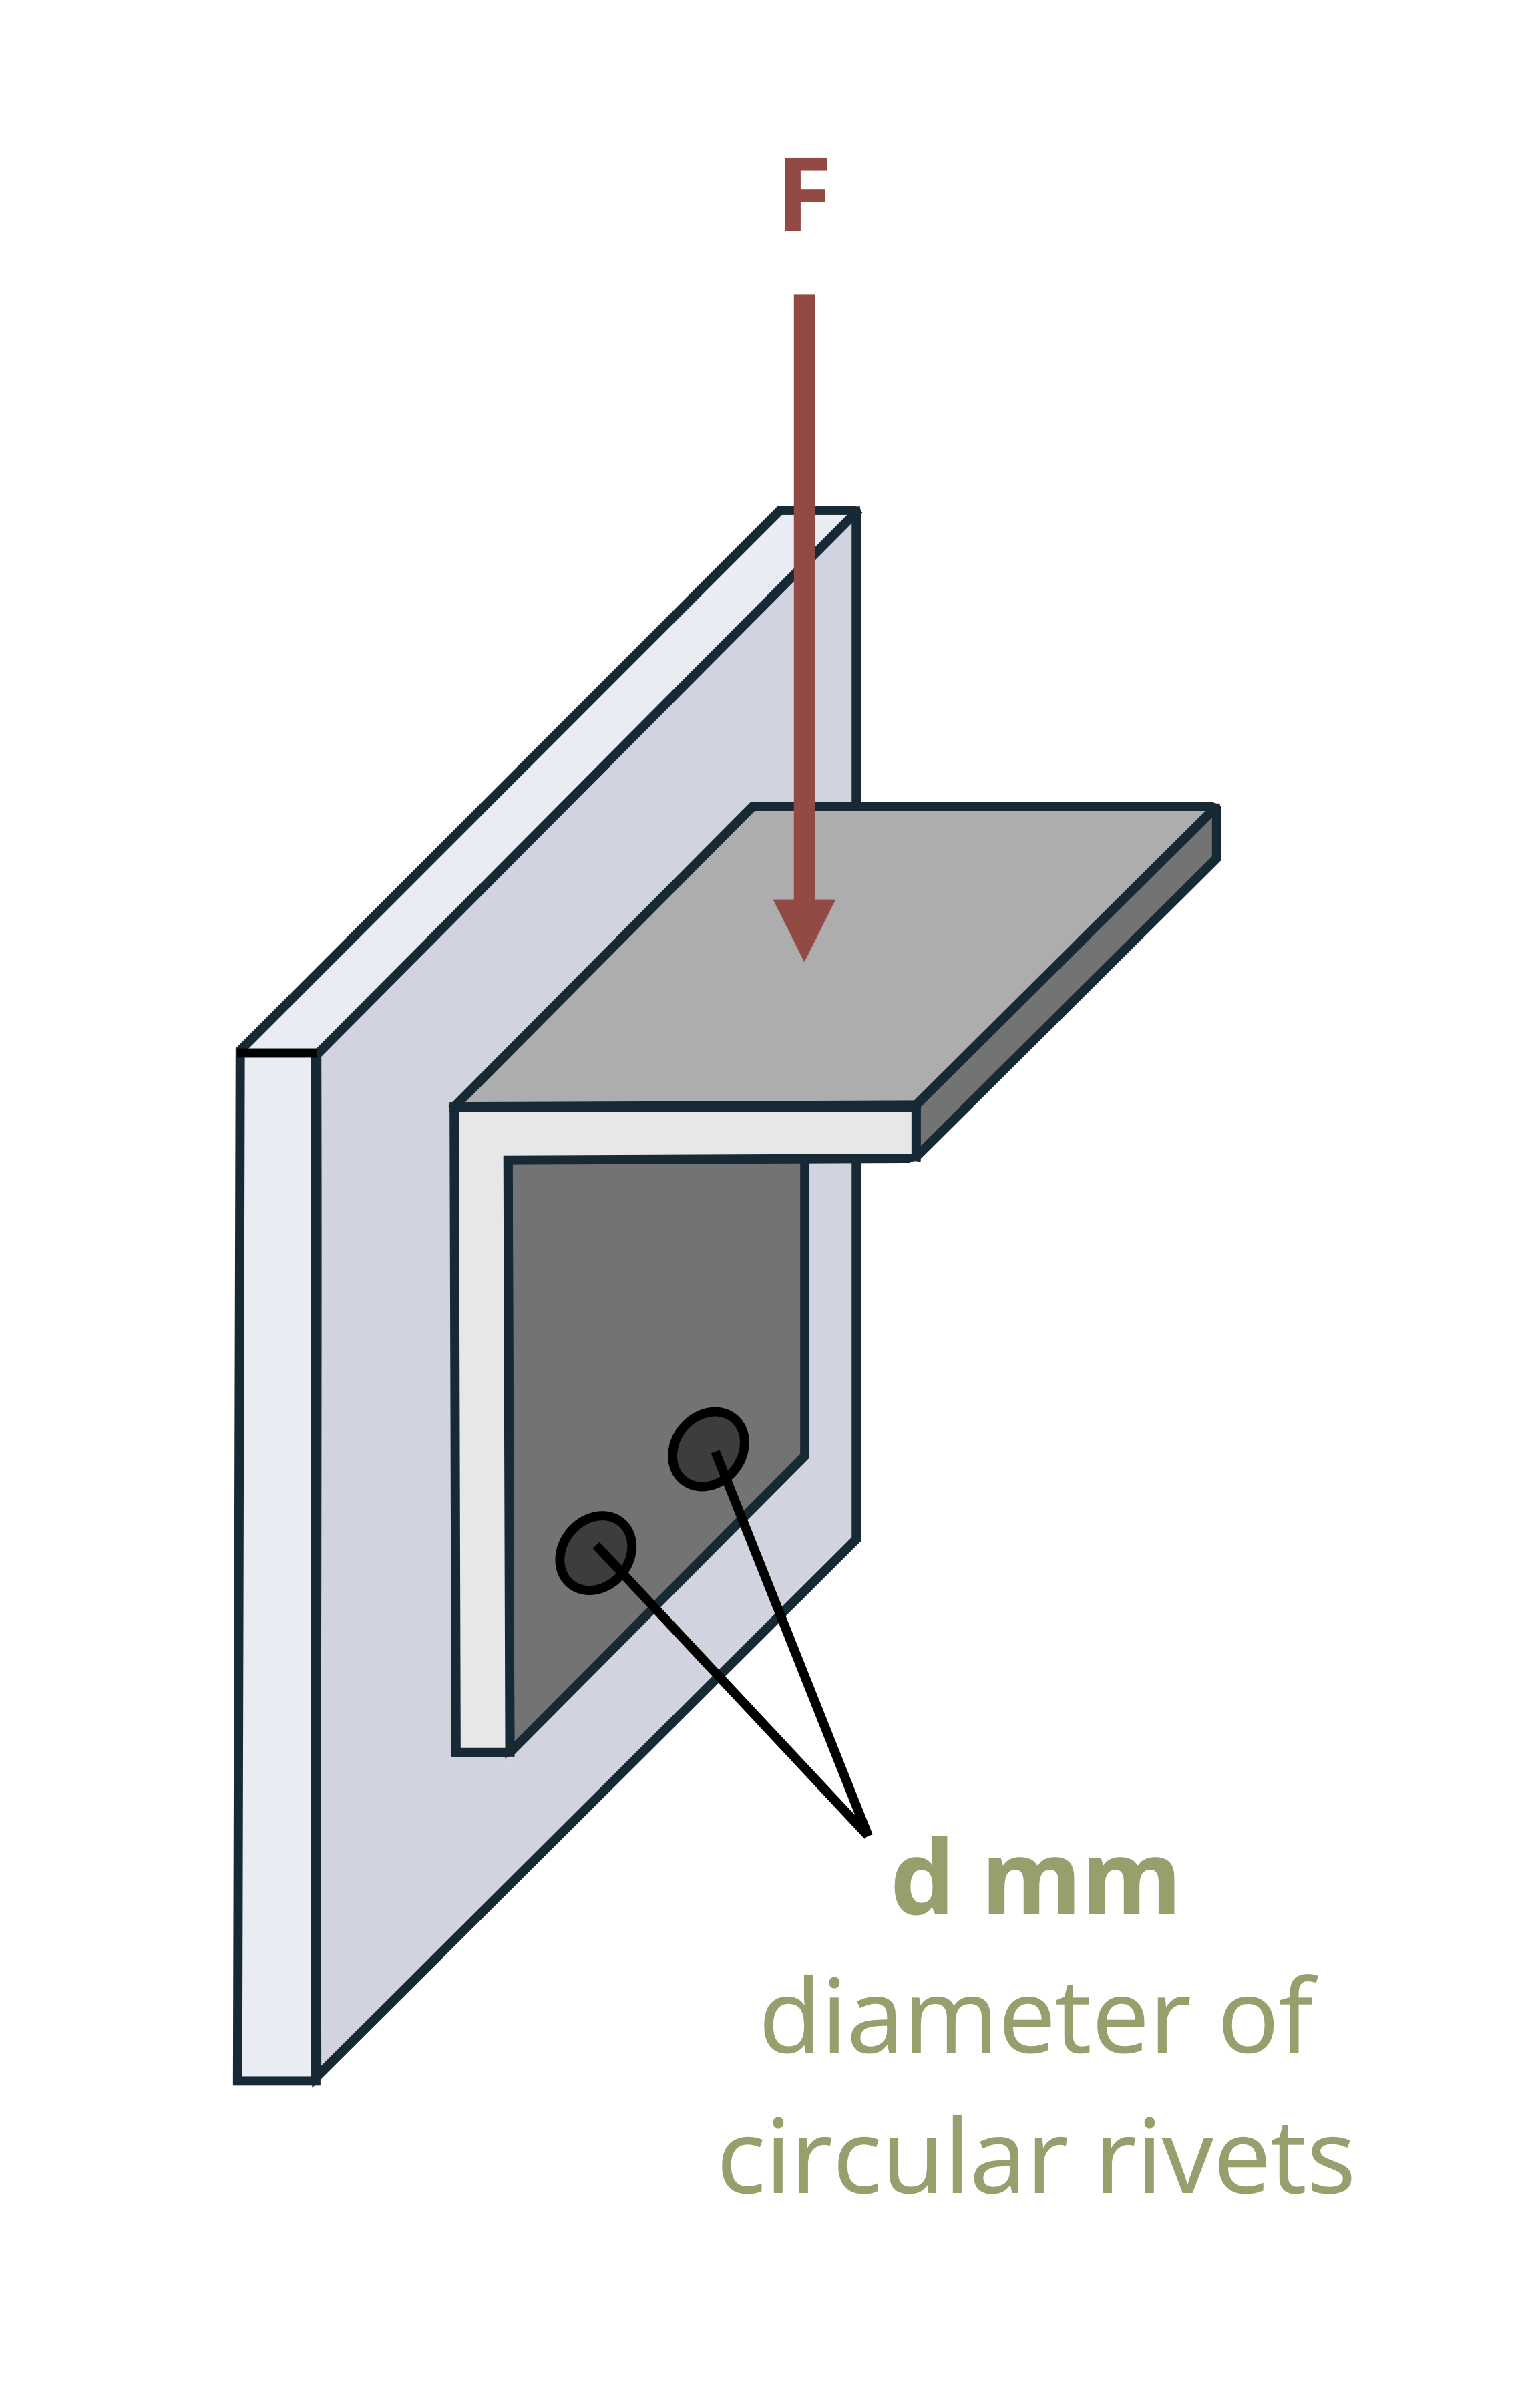
\includegraphics{images/165.png}

}

\caption{Figure 1: A bracket is attached to a wall with two circular
rivets.}

\end{figure}%

\begin{Shaded}
\begin{Highlighting}[]
\NormalTok{\#| standalone: true}
\NormalTok{\#| viewerHeight: 600}
\NormalTok{\#| components: [viewer]}

\NormalTok{from shiny import App, render, ui, reactive}
\NormalTok{import random}
\NormalTok{import asyncio}
\NormalTok{import io}
\NormalTok{import math}
\NormalTok{import string}
\NormalTok{from datetime import datetime}
\NormalTok{from pathlib import Path}

\NormalTok{def generate\_random\_letters(length):}
\NormalTok{    \# Generate a random string of letters of specified length}
\NormalTok{    return \textquotesingle{}\textquotesingle{}.join(random.choice(string.ascii\_lowercase) for \_ in range(length))}

\NormalTok{problem\_ID="165"}
\NormalTok{F=reactive.Value("\_\_")}
\NormalTok{d=reactive.Value("\_\_")}


\NormalTok{attempts=["Timestamp,Attempt,Answer,Feedback\textbackslash{}n"]}

\NormalTok{app\_ui = ui.page\_fluid(}
\NormalTok{    ui.markdown("**Please enter your ID number from your instructor and click to generate your problem**"),}
\NormalTok{    ui.input\_text("ID","", placeholder="Enter ID Number Here"),}
\NormalTok{    ui.input\_action\_button("generate\_problem", "Generate Problem", class\_="btn{-}primary"),}
\NormalTok{    ui.markdown("**Problem Statement**"),}
\NormalTok{    ui.output\_ui("ui\_problem\_statement"),}
\NormalTok{    ui.input\_text("answer","Your Answer in units of MPa", placeholder="Please enter your answer"),}
\NormalTok{    ui.input\_action\_button("submit", "Submit Answer", class\_="btn{-}primary"),}
\NormalTok{    ui.download\_button("download", "Download File to Submit", class\_="btn{-}success"),}
\NormalTok{)}


\NormalTok{def server(input, output, session):}
\NormalTok{    \# Initialize a counter for attempts}
\NormalTok{    attempt\_counter = reactive.Value(0)}

\NormalTok{    @output}
\NormalTok{    @render.ui}
\NormalTok{    def ui\_problem\_statement():}
\NormalTok{        return[ui.markdown(f"A bracket is attached to a wall with two circular rivets of diameter d = \{d()\} mm. A load F = \{F()\} kN is applied in the center of the bracket. Assuming the load is split evenly between the two rivits, determine the shear stress in each rivet. ")]}
    
\NormalTok{    @reactive.Effect}
\NormalTok{    @reactive.event(input.generate\_problem)}
\NormalTok{    def randomize\_vars():}
\NormalTok{        random.seed(input.ID())}
\NormalTok{        F.set(random.randrange(30, 100, 1))}
\NormalTok{        d.set(random.randrange(10, 40, 1))}
        

\NormalTok{    @reactive.Effect}
\NormalTok{    @reactive.event(input.submit)}
\NormalTok{    def \_():}
\NormalTok{        attempt\_counter.set(attempt\_counter() + 1)  \# Increment the attempt counter on each submission.  }
      
\NormalTok{        A = math.pi*(d()/(1000*2))**2}
\NormalTok{        instr= ((F()/2)/A)/1000}
\NormalTok{        if math.isclose(float(input.answer()), instr, rel\_tol=0.01):}
\NormalTok{            check = "*Correct*"}
\NormalTok{            correct\_indicator = "JL"}
\NormalTok{        else:}
\NormalTok{            check = "*Not Correct.*"}
\NormalTok{            correct\_indicator = "JG"}

\NormalTok{        \# Generate random parts for the encoded attempt.}
\NormalTok{        random\_start = generate\_random\_letters(4)}
\NormalTok{        random\_middle = generate\_random\_letters(4)}
\NormalTok{        random\_end = generate\_random\_letters(4)}
\NormalTok{        encoded\_attempt = f"\{random\_start\}\{problem\_ID\}{-}\{random\_middle\}\{attempt\_counter()\}\{correct\_indicator\}{-}\{random\_end\}\{input.ID()\}"}

\NormalTok{        \# Store the most recent encoded attempt in a reactive value so it persists across submissions}
\NormalTok{        session.encoded\_attempt = reactive.Value(encoded\_attempt)}

\NormalTok{        \# Append the attempt data to the attempts list without the encoded attempt}
\NormalTok{        attempts.append(f"\{datetime.now()\}, \{attempt\_counter()\}, \{input.answer()\}, \{check\}\textbackslash{}n")}

\NormalTok{        \# Show feedback to the user.}
\NormalTok{        feedback = ui.markdown(f"Your answer of \{input.answer()\} is \{check\}.")}
\NormalTok{        m = ui.modal(}
\NormalTok{            feedback,}
\NormalTok{            title="Feedback",}
\NormalTok{            easy\_close=True}
\NormalTok{        )}
\NormalTok{        ui.modal\_show(m)}

\NormalTok{    @session.download(filename=lambda: f"Problem\_Log{-}\{problem\_ID\}{-}\{input.ID()\}.csv")}
\NormalTok{    async def download():}
\NormalTok{        \# Start the CSV with the encoded attempt (without label)}
\NormalTok{        final\_encoded = session.encoded\_attempt() if session.encoded\_attempt is not None else "No attempts"}
\NormalTok{        yield f"\{final\_encoded\}\textbackslash{}n\textbackslash{}n"}
        
\NormalTok{        \# Write the header for the remaining CSV data once}
\NormalTok{        yield "Timestamp,Attempt,Answer,Feedback\textbackslash{}n"}
        
\NormalTok{        \# Write the attempts data, ensure that the header from the attempts list is not written again}
\NormalTok{        for attempt in attempts[1:]:  \# Skip the first element which is the header}
\NormalTok{            await asyncio.sleep(0.25)  \# This delay may not be necessary; adjust as needed}
\NormalTok{            yield attempt}


\NormalTok{\# App installation}
\NormalTok{app = App(app\_ui, server)}
\end{Highlighting}
\end{Shaded}

\chapter*{Problem 2.23}\label{problem-2.23}
\addcontentsline{toc}{chapter}{Problem 2.23}

\markboth{Problem 2.23}{Problem 2.23}

This is a dynamic rendering of the problem with dynamic variables based
on the username entered.

\section*{Problem Image}\label{problem-image-26}
\addcontentsline{toc}{section}{Problem Image}

\markright{Problem Image}

\begin{figure}[H]

{\centering 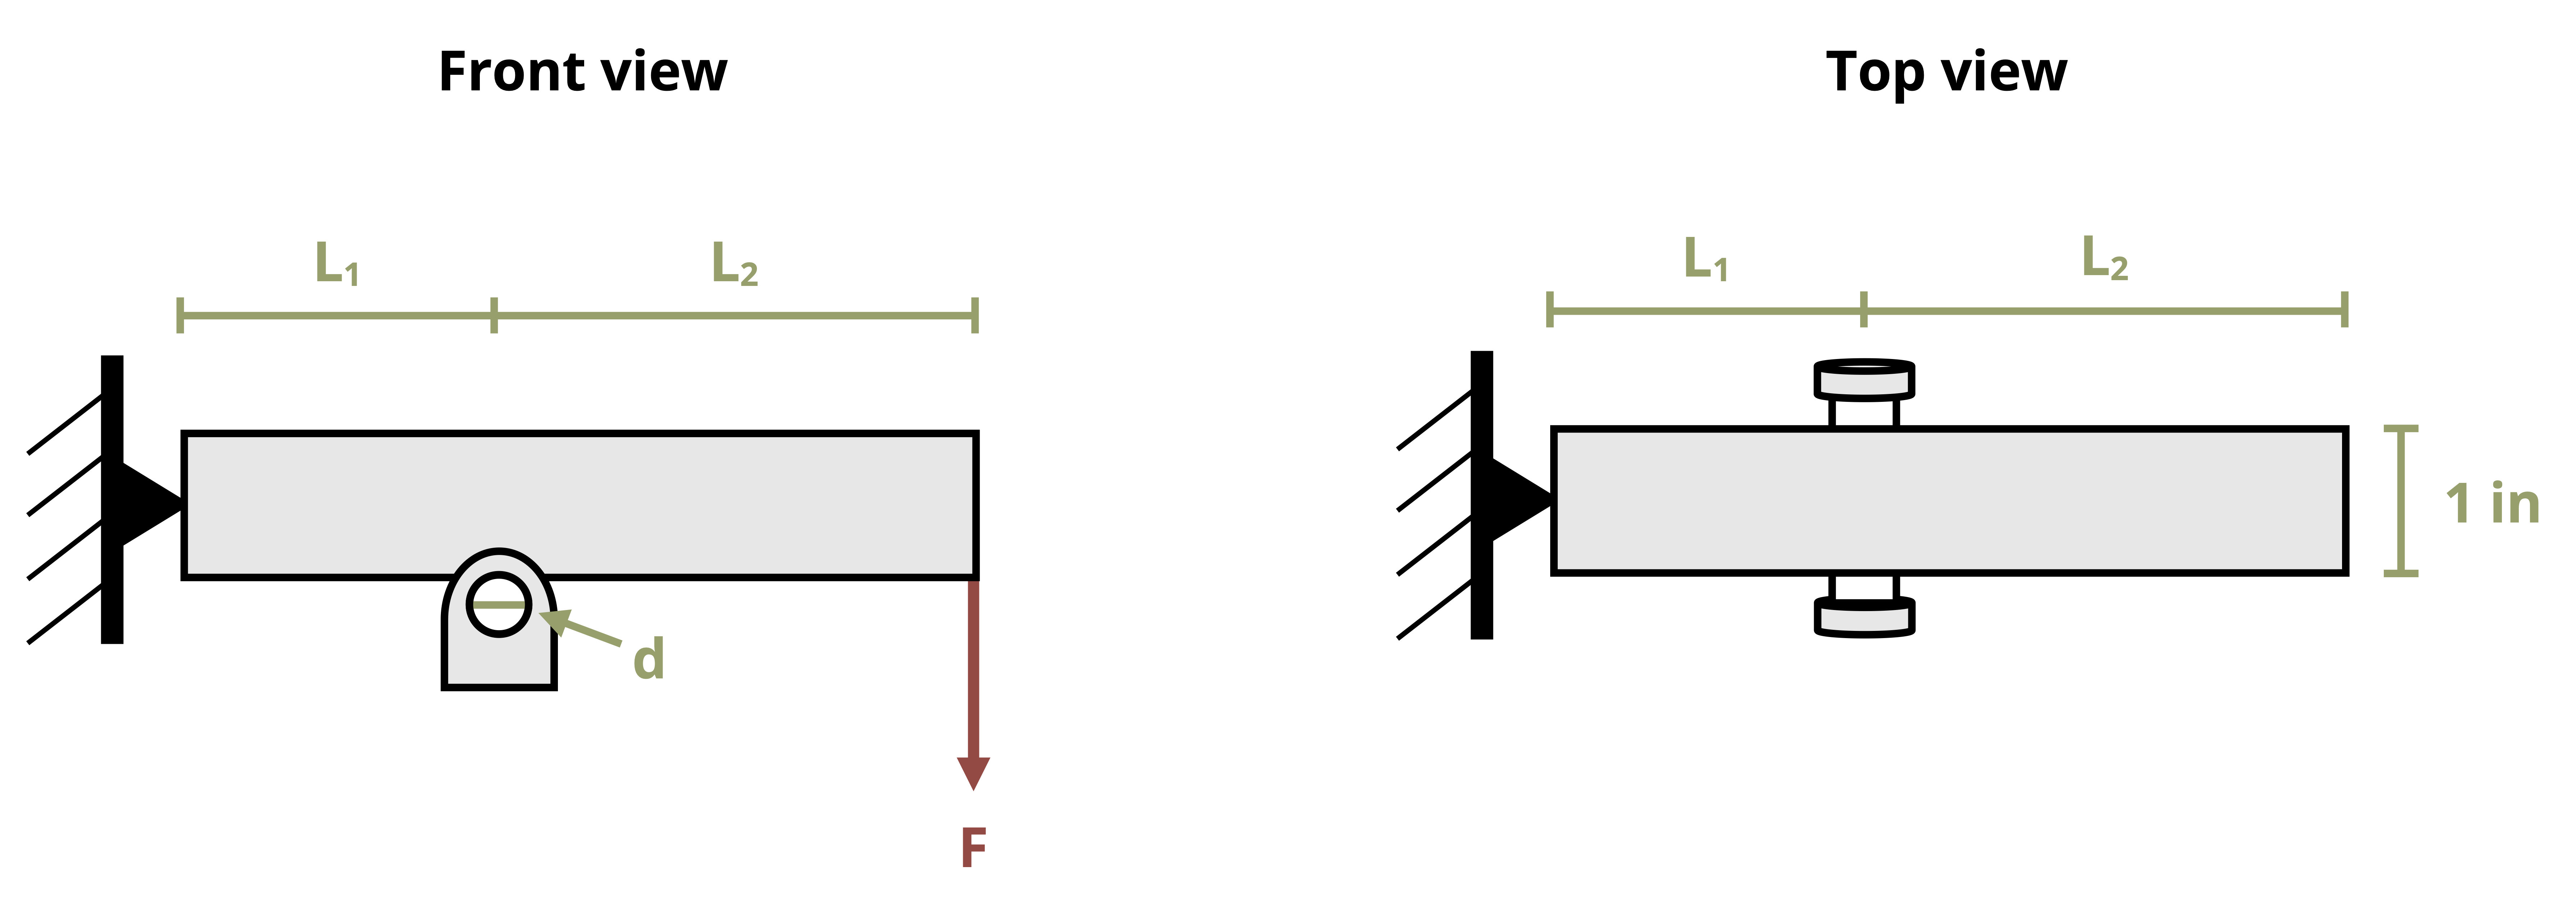
\includegraphics{images/168.png}

}

\caption{Figure 1: A square bar of length is pinned at one end and rests
on a circular rod.}

\end{figure}%

\begin{Shaded}
\begin{Highlighting}[]
\NormalTok{\#| standalone: true}
\NormalTok{\#| viewerHeight: 600}
\NormalTok{\#| components: [viewer]}

\NormalTok{from shiny import App, render, ui, reactive}
\NormalTok{import random}
\NormalTok{import asyncio}
\NormalTok{import io}
\NormalTok{import math}
\NormalTok{import string}
\NormalTok{from datetime import datetime}
\NormalTok{from pathlib import Path}

\NormalTok{def generate\_random\_letters(length):}
\NormalTok{    \# Generate a random string of letters of specified length}
\NormalTok{    return \textquotesingle{}\textquotesingle{}.join(random.choice(string.ascii\_lowercase) for \_ in range(length)) }

\NormalTok{problem\_ID="168"}
\NormalTok{L1=reactive.Value("\_\_")}
\NormalTok{L2=reactive.Value("\_\_")}
\NormalTok{d=reactive.Value("\_\_")}
\NormalTok{F=reactive.Value("\_\_")}

\NormalTok{attempts=["Timestamp,Attempt,Answer,Feedback\textbackslash{}n"]}

\NormalTok{app\_ui = ui.page\_fluid(}
\NormalTok{    ui.markdown("**Please enter your ID number from your instructor and click to generate your problem**"),}
\NormalTok{    ui.input\_text("ID","", placeholder="Enter ID Number Here"),}
\NormalTok{    ui.input\_action\_button("generate\_problem", "Generate Problem", class\_="btn{-}primary"),}
\NormalTok{    ui.markdown("**Problem Statement**"),}
\NormalTok{    ui.output\_ui("ui\_problem\_statement"),}
\NormalTok{    ui.input\_text("answer","Your Answer in units of psi", placeholder="Please enter your answer"),}
\NormalTok{    ui.input\_action\_button("submit", "Submit Answer", class\_="btn{-}primary"),}
\NormalTok{    ui.download\_button("download", "Download File to Submit", class\_="btn{-}success"),}
\NormalTok{)}

\NormalTok{def server(input, output, session):}
\NormalTok{    \# Initialize a counter for attempts}
\NormalTok{    attempt\_counter = reactive.Value(0)}

\NormalTok{    @output}
\NormalTok{    @render.ui}
\NormalTok{    def ui\_problem\_statement():}
\NormalTok{        return[ui.markdown(f"A square bar of length L\textless{}sub\textgreater{}1\textless{}/sub\textgreater{} = \{L1()\} in. and L\textless{}sub\textgreater{}2\textless{}/sub\textgreater{} = \{L2()\} in. is pinned at one end and rests on a circular rod of diameter d = \{d()\} in. A force F = \{F()\} lb is applied at the free end. What is the average shear stress in the circular rod? ")]}
    
\NormalTok{    @reactive.Effect}
\NormalTok{    @reactive.event(input.generate\_problem)}
\NormalTok{    def randomize\_vars():}
\NormalTok{        random.seed(input.ID())}
\NormalTok{        L1.set(random.randrange(50, 150, 1)/10)}
\NormalTok{        L2.set(round(L1() * 1.4, 1))}
\NormalTok{        d.set(random.randrange(4, 9, 1)/10)}
\NormalTok{        F.set(random.randrange(30, 100, 1))}

\NormalTok{    @reactive.Effect}
\NormalTok{    @reactive.event(input.submit)}
\NormalTok{    def \_():}
\NormalTok{        attempt\_counter.set(attempt\_counter() + 1)  \# Increment the attempt counter on each submission.}
    
\NormalTok{        M = F()*(L1()+L2())}
\NormalTok{        R = M/L1()}
\NormalTok{        A = math.pi*(d()/2)**2}
\NormalTok{        instr= R/(2*A)}
\NormalTok{        if math.isclose(float(input.answer()), instr, rel\_tol=0.01):}
\NormalTok{            check = "*Correct*"}
\NormalTok{            correct\_indicator = "JL"}
\NormalTok{        else:}
\NormalTok{            check = "*Not Correct.*"}
\NormalTok{            correct\_indicator = "JG"}

\NormalTok{        \# Generate random parts for the encoded attempt.}
\NormalTok{        random\_start = generate\_random\_letters(4)}
\NormalTok{        random\_middle = generate\_random\_letters(4)}
\NormalTok{        random\_end = generate\_random\_letters(4)}
\NormalTok{        encoded\_attempt = f"\{random\_start\}\{problem\_ID\}{-}\{random\_middle\}\{attempt\_counter()\}\{correct\_indicator\}{-}\{random\_end\}\{input.ID()\}"}

\NormalTok{        \# Store the most recent encoded attempt in a reactive value so it persists across submissions}
\NormalTok{        session.encoded\_attempt = reactive.Value(encoded\_attempt)}

\NormalTok{        \# Append the attempt data to the attempts list without the encoded attempt}
\NormalTok{        attempts.append(f"\{datetime.now()\}, \{attempt\_counter()\}, \{input.answer()\}, \{check\}\textbackslash{}n")}

\NormalTok{        \# Show feedback to the user.}
\NormalTok{        feedback = ui.markdown(f"Your answer of \{input.answer()\} is \{check\}.")}
\NormalTok{        m = ui.modal(}
\NormalTok{            feedback,}
\NormalTok{            title="Feedback",}
\NormalTok{            easy\_close=True}
\NormalTok{        )}
\NormalTok{        ui.modal\_show(m)}

\NormalTok{    @session.download(filename=lambda: f"Problem\_Log{-}\{problem\_ID\}{-}\{input.ID()\}.csv")}
\NormalTok{    async def download():}
\NormalTok{        \# Start the CSV with the encoded attempt (without label)}
\NormalTok{        final\_encoded = session.encoded\_attempt() if session.encoded\_attempt is not None else "No attempts"}
\NormalTok{        yield f"\{final\_encoded\}\textbackslash{}n\textbackslash{}n"}
        
\NormalTok{        \# Write the header for the remaining CSV data once}
\NormalTok{        yield "Timestamp,Attempt,Answer,Feedback\textbackslash{}n"}
        
\NormalTok{        \# Write the attempts data, ensure that the header from the attempts list is not written again}
\NormalTok{        for attempt in attempts[1:]:  \# Skip the first element which is the header}
\NormalTok{            await asyncio.sleep(0.25)  \# This delay may not be necessary; adjust as needed}
\NormalTok{            yield attempt}

\NormalTok{\# App installation}
\NormalTok{app = App(app\_ui, server)}
\end{Highlighting}
\end{Shaded}

\chapter*{Problem 2.38}\label{problem-2.38-2}
\addcontentsline{toc}{chapter}{Problem 2.38}

\markboth{Problem 2.38}{Problem 2.38}

This is a dynamic rendering of the problem with dynamic variables based
on the username entered.

\section*{Problem Image}\label{problem-image-27}
\addcontentsline{toc}{section}{Problem Image}

\markright{Problem Image}

\begin{figure}[H]

{\centering 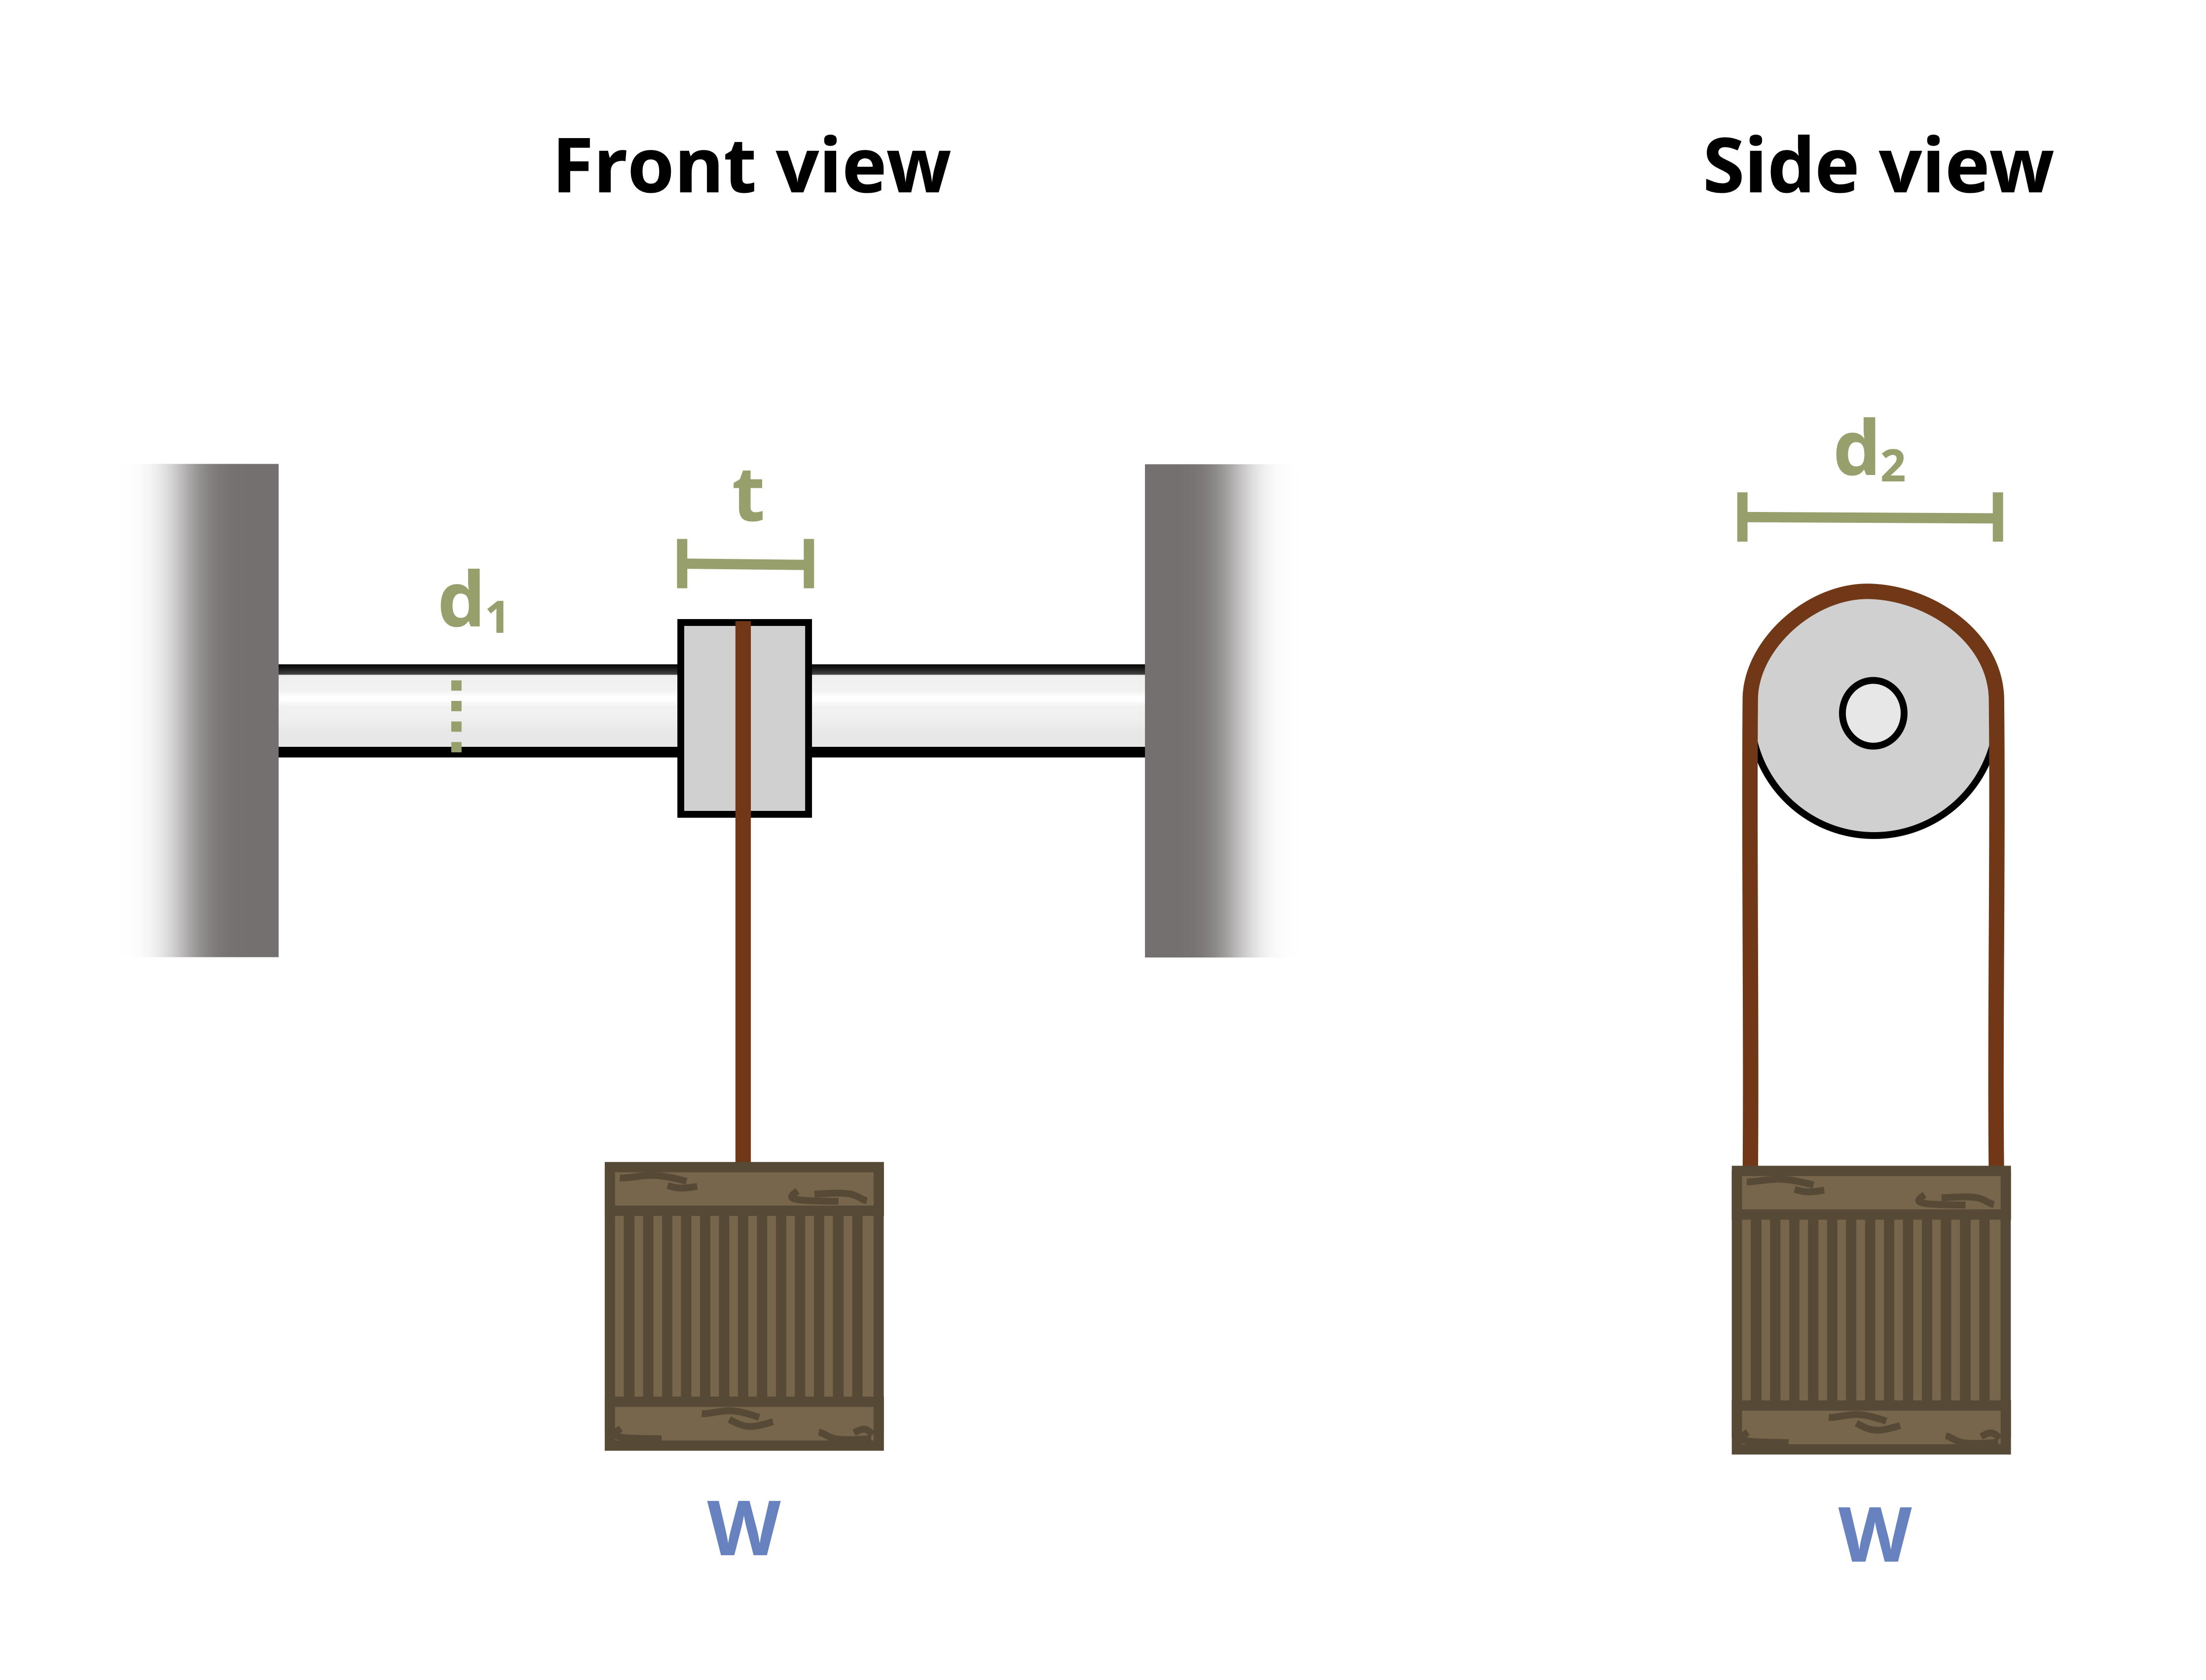
\includegraphics{images/166.png}

}

\caption{Figure 1: A crate is hung on a circular solid metal rod.}

\end{figure}%

\begin{Shaded}
\begin{Highlighting}[]
\NormalTok{\#| standalone: true}
\NormalTok{\#| viewerHeight: 600}
\NormalTok{\#| components: [viewer]}
\NormalTok{from shiny import App, render, ui, reactive}
\NormalTok{import random}
\NormalTok{import asyncio}
\NormalTok{import io}
\NormalTok{import math}
\NormalTok{import string}
\NormalTok{from datetime import datetime}
\NormalTok{from pathlib import Path}

\NormalTok{def generate\_random\_letters(length):}
\NormalTok{    \# Generate a random string of letters of specified length}
\NormalTok{    return \textquotesingle{}\textquotesingle{}.join(random.choice(string.ascii\_lowercase) for \_ in range(length))}

\NormalTok{problem\_ID="166"}
\NormalTok{W=reactive.Value("\_\_")}
\NormalTok{d1=reactive.Value("\_\_")}
\NormalTok{d2=reactive.Value("\_\_")}
\NormalTok{t=reactive.Value("\_\_")}
\NormalTok{attempts=["Timestamp,Attempt,Answer,Feedback\textbackslash{}n"]}

\NormalTok{app\_ui = ui.page\_fluid(}
\NormalTok{    ui.markdown("**Please enter your ID number from your instructor and click to generate your problem**"),}
\NormalTok{    ui.input\_text("ID","", placeholder="Enter ID Number Here"),}
\NormalTok{    ui.input\_action\_button("generate\_problem", "Generate Problem", class\_="btn{-}primary"),}
\NormalTok{    ui.markdown("**Problem Statement**"),}
\NormalTok{    ui.output\_ui("ui\_problem\_statement"),}
\NormalTok{    ui.input\_text("answer","Your Answer in units of ksi", placeholder="Please enter your answer"),}
\NormalTok{    ui.input\_action\_button("submit", "Submit Answer", class\_="btn{-}primary"),}
\NormalTok{    ui.download\_button("download", "Download File to Submit", class\_="btn{-}success"),}
\NormalTok{)}


\NormalTok{def server(input, output, session):}
\NormalTok{    \# Initialize a counter for attempts}
\NormalTok{    attempt\_counter = reactive.Value(0)}
    
\NormalTok{    @output}
\NormalTok{    @render.ui}
\NormalTok{    def ui\_problem\_statement():}
\NormalTok{        return[ui.markdown(f"A crate of weight \{W()\} = lb hangs from a solid circular metal rod of diameter \{d1()\} = in.. The cable is wrapped around a support collar of diameter \{d2()\} = in. and thickness \{t()\} = in. to evenly distribute the cable load. What is the bearing stress on the support collar due to the rod? ")]}
    
\NormalTok{    @reactive.Effect}
\NormalTok{    @reactive.event(input.generate\_problem)}
\NormalTok{    def randomize\_vars():}
\NormalTok{        random.seed(input.ID())}
\NormalTok{        W.set(random.randrange(4000, 9000, 100))}
\NormalTok{        d1.set(random.randrange(5, 30, 1)/10)}
\NormalTok{        d2.set(d1()*3)}
\NormalTok{        t.set(d1()*2)}
\NormalTok{    @reactive.Effect}
\NormalTok{    @reactive.event(input.submit)}
\NormalTok{    def \_():}
        
\NormalTok{        instr= W()/(d1()*t()*1000)}
        
\NormalTok{        if math.isclose(float(input.answer()), instr, rel\_tol=0.01):}
\NormalTok{            check = "*Correct*"}
\NormalTok{            correct\_indicator = "JL"}
\NormalTok{        else:}
\NormalTok{            check = "*Not Correct.*"}
\NormalTok{            correct\_indicator = "JG"}

\NormalTok{        \# Generate random parts for the encoded attempt.}
\NormalTok{        random\_start = generate\_random\_letters(4)}
\NormalTok{        random\_middle = generate\_random\_letters(4)}
\NormalTok{        random\_end = generate\_random\_letters(4)}
\NormalTok{        encoded\_attempt = f"\{random\_start\}\{problem\_ID\}{-}\{random\_middle\}\{attempt\_counter()\}\{correct\_indicator\}{-}\{random\_end\}\{input.ID()\}"}

\NormalTok{        \# Store the most recent encoded attempt in a reactive value so it persists across submissions}
\NormalTok{        session.encoded\_attempt = reactive.Value(encoded\_attempt)}

\NormalTok{        \# Append the attempt data to the attempts list without the encoded attempt}
\NormalTok{        attempts.append(f"\{datetime.now()\}, \{attempt\_counter()\}, \{input.answer()\}, \{check\}\textbackslash{}n")}

\NormalTok{        \# Show feedback to the user.}
\NormalTok{        feedback = ui.markdown(f"Your answer of \{input.answer()\} is \{check\}.")}
\NormalTok{        m = ui.modal(}
\NormalTok{            feedback,}
\NormalTok{            title="Feedback",}
\NormalTok{            easy\_close=True}
\NormalTok{        )}
\NormalTok{        ui.modal\_show(m)}

\NormalTok{    @session.download(filename=lambda: f"Problem\_Log{-}\{problem\_ID\}{-}\{input.ID()\}.csv")}
\NormalTok{    async def download():}
\NormalTok{        \# Start the CSV with the encoded attempt (without label)}
\NormalTok{        final\_encoded = session.encoded\_attempt() if session.encoded\_attempt is not None else "No attempts"}
\NormalTok{        yield f"\{final\_encoded\}\textbackslash{}n\textbackslash{}n"}
        
\NormalTok{        \# Write the header for the remaining CSV data once}
\NormalTok{        yield "Timestamp,Attempt,Answer,Feedback\textbackslash{}n"}
        
\NormalTok{        \# Write the attempts data, ensure that the header from the attempts list is not written again}
\NormalTok{        for attempt in attempts[1:]:  \# Skip the first element which is the header}
\NormalTok{            await asyncio.sleep(0.25)  \# This delay may not be necessary; adjust as needed}
\NormalTok{            yield attempt}


\NormalTok{\# App installation}
\NormalTok{app = App(app\_ui, server)}
\end{Highlighting}
\end{Shaded}

\chapter*{Problem 2.39}\label{problem-2.39}
\addcontentsline{toc}{chapter}{Problem 2.39}

\markboth{Problem 2.39}{Problem 2.39}

This is a dynamic rendering of the problem with dynamic variables based
on the username entered.

\section*{Problem Image}\label{problem-image-28}
\addcontentsline{toc}{section}{Problem Image}

\markright{Problem Image}

\begin{figure}[H]

{\centering 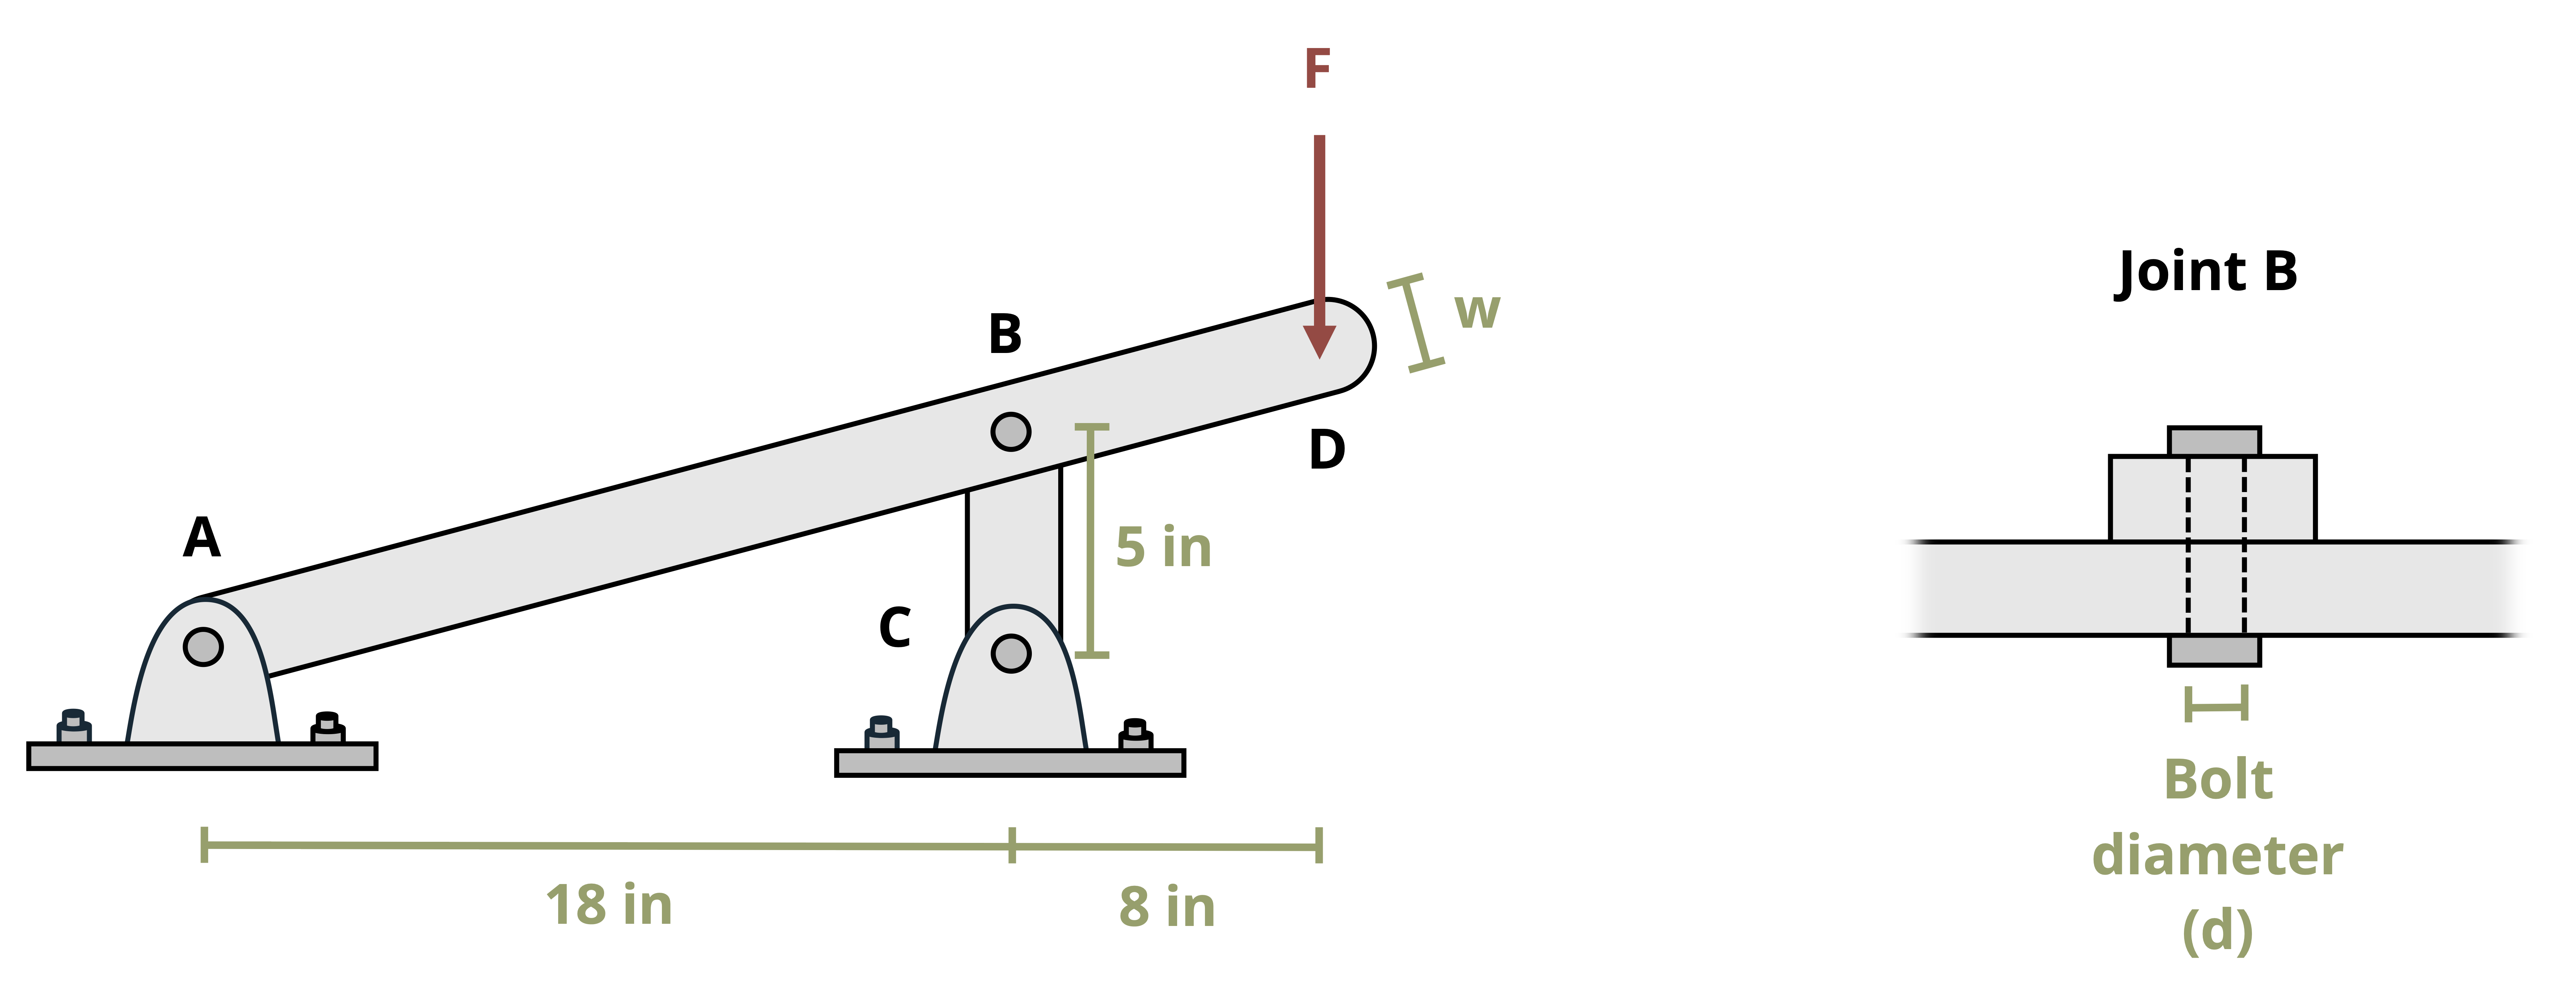
\includegraphics{images/180.png}

}

\caption{Figure 1: A link mechanism is connected with pins.}

\end{figure}%

\begin{Shaded}
\begin{Highlighting}[]
\NormalTok{\#| standalone: true}
\NormalTok{\#| viewerHeight: 600}
\NormalTok{\#| components: [viewer]}

\NormalTok{from shiny import App, render, ui, reactive}
\NormalTok{import random}
\NormalTok{import asyncio}
\NormalTok{import io}
\NormalTok{import math}
\NormalTok{import string}
\NormalTok{from datetime import datetime}
\NormalTok{from pathlib import Path}

\NormalTok{def generate\_random\_letters(length):}
\NormalTok{    \# Generate a random string of letters of specified length}
\NormalTok{    return \textquotesingle{}\textquotesingle{}.join(random.choice(string.ascii\_lowercase) for \_ in range(length)) }

\NormalTok{problem\_ID="180"}
\NormalTok{F=reactive.Value("\_\_")}
\NormalTok{d=reactive.Value("\_\_")}
\NormalTok{t=reactive.Value("\_\_")}
\NormalTok{w=reactive.Value("\_\_")}



\NormalTok{attempts=["Timestamp,Attempt,Answer,Feedback\textbackslash{}n"]}

\NormalTok{app\_ui = ui.page\_fluid(}
\NormalTok{    ui.markdown("**Please enter your ID number from your instructor and click to generate your problem**"),}
\NormalTok{    ui.input\_text("ID","", placeholder="Enter ID Number Here"),}
\NormalTok{    ui.input\_action\_button("generate\_problem", "Generate Problem", class\_="btn{-}primary"),}
\NormalTok{    ui.markdown("**Problem Statement**"),}
\NormalTok{    ui.output\_ui("ui\_problem\_statement"),}
\NormalTok{    ui.input\_text("answer","Your Answer in units of ksi", placeholder="Please enter your answer"),}
\NormalTok{    ui.input\_action\_button("submit", "Submit Answer", class\_="btn{-}primary"),}
\NormalTok{    ui.download\_button("download", "Download File to Submit", class\_="btn{-}success"),}
\NormalTok{)}


\NormalTok{def server(input, output, session):}
\NormalTok{    \# Initialize a counter for attempts}
\NormalTok{    attempt\_counter = reactive.Value(0)  }
  
\NormalTok{    @output}
\NormalTok{    @render.ui}
\NormalTok{    def ui\_problem\_statement():}
\NormalTok{        return[ui.markdown(f"A link mechanism is connected with pins of diameter d = \{d()\} in. A force F = \{F()\} lb is applied to the mechanism as shown. The mechanism has width w = \{w()\} in. and thickness t = \{t()\} in. What is the bearing stress in member BC at joint B due to the pin at B? ")]}
    
\NormalTok{    @reactive.Effect}
\NormalTok{    @reactive.event(input.generate\_problem)}
\NormalTok{    def randomize\_vars():}
\NormalTok{        random.seed(input.ID())}
\NormalTok{        F.set(random.randrange(200, 900, 10))}
\NormalTok{        d.set(random.randrange(20, 150, 10)/100)}
\NormalTok{        t.set(random.randrange(2, 10, 1)/10)}
\NormalTok{        w.set(round(d()*2, 2))}
        

\NormalTok{    @reactive.Effect}
\NormalTok{    @reactive.event(input.submit)}
\NormalTok{    def \_():}
\NormalTok{        attempt\_counter.set(attempt\_counter() + 1)  \# Increment the attempt counter on each submission.}
\NormalTok{        Fb=((18+8)*F())/18}
\NormalTok{        instr= Fb/(d()*t())/1000}
\NormalTok{        if math.isclose(float(input.answer()), instr, rel\_tol=0.01):}
\NormalTok{            check = "*Correct*"}
\NormalTok{            correct\_indicator = "JL"}
\NormalTok{        else:}
\NormalTok{            check = "*Not Correct.*"}
\NormalTok{            correct\_indicator = "JG"}

\NormalTok{        \# Generate random parts for the encoded attempt.}
\NormalTok{        random\_start = generate\_random\_letters(4)}
\NormalTok{        random\_middle = generate\_random\_letters(4)}
\NormalTok{        random\_end = generate\_random\_letters(4)}
\NormalTok{        encoded\_attempt = f"\{random\_start\}\{problem\_ID\}{-}\{random\_middle\}\{attempt\_counter()\}\{correct\_indicator\}{-}\{random\_end\}\{input.ID()\}"}

\NormalTok{        \# Store the most recent encoded attempt in a reactive value so it persists across submissions}
\NormalTok{        session.encoded\_attempt = reactive.Value(encoded\_attempt)}

\NormalTok{        \# Append the attempt data to the attempts list without the encoded attempt}
\NormalTok{        attempts.append(f"\{datetime.now()\}, \{attempt\_counter()\}, \{input.answer()\}, \{check\}\textbackslash{}n")}

\NormalTok{        \# Show feedback to the user.}
\NormalTok{        feedback = ui.markdown(f"Your answer of \{input.answer()\} is \{check\}.")}
\NormalTok{        m = ui.modal(}
\NormalTok{            feedback,}
\NormalTok{            title="Feedback",}
\NormalTok{            easy\_close=True}
\NormalTok{        )}
\NormalTok{        ui.modal\_show(m)}

\NormalTok{    @session.download(filename=lambda: f"Problem\_Log{-}\{problem\_ID\}{-}\{input.ID()\}.csv")}
\NormalTok{    async def download():}
\NormalTok{        \# Start the CSV with the encoded attempt (without label)}
\NormalTok{        final\_encoded = session.encoded\_attempt() if session.encoded\_attempt is not None else "No attempts"}
\NormalTok{        yield f"\{final\_encoded\}\textbackslash{}n\textbackslash{}n"}
        
\NormalTok{        \# Write the header for the remaining CSV data once}
\NormalTok{        yield "Timestamp,Attempt,Answer,Feedback\textbackslash{}n"}
        
\NormalTok{        \# Write the attempts data, ensure that the header from the attempts list is not written again}
\NormalTok{        for attempt in attempts[1:]:  \# Skip the first element which is the header}
\NormalTok{            await asyncio.sleep(0.25)  \# This delay may not be necessary; adjust as needed}
\NormalTok{            yield attempt}


\NormalTok{\# App installation}
\NormalTok{app = App(app\_ui, server)}
\end{Highlighting}
\end{Shaded}

\chapter*{Problem 2.40}\label{problem-2.40}
\addcontentsline{toc}{chapter}{Problem 2.40}

\markboth{Problem 2.40}{Problem 2.40}

This is a dynamic rendering of the problem with dynamic variables based
on the username entered.

\section*{Problem Image}\label{problem-image-29}
\addcontentsline{toc}{section}{Problem Image}

\markright{Problem Image}

\begin{figure}[H]

{\centering 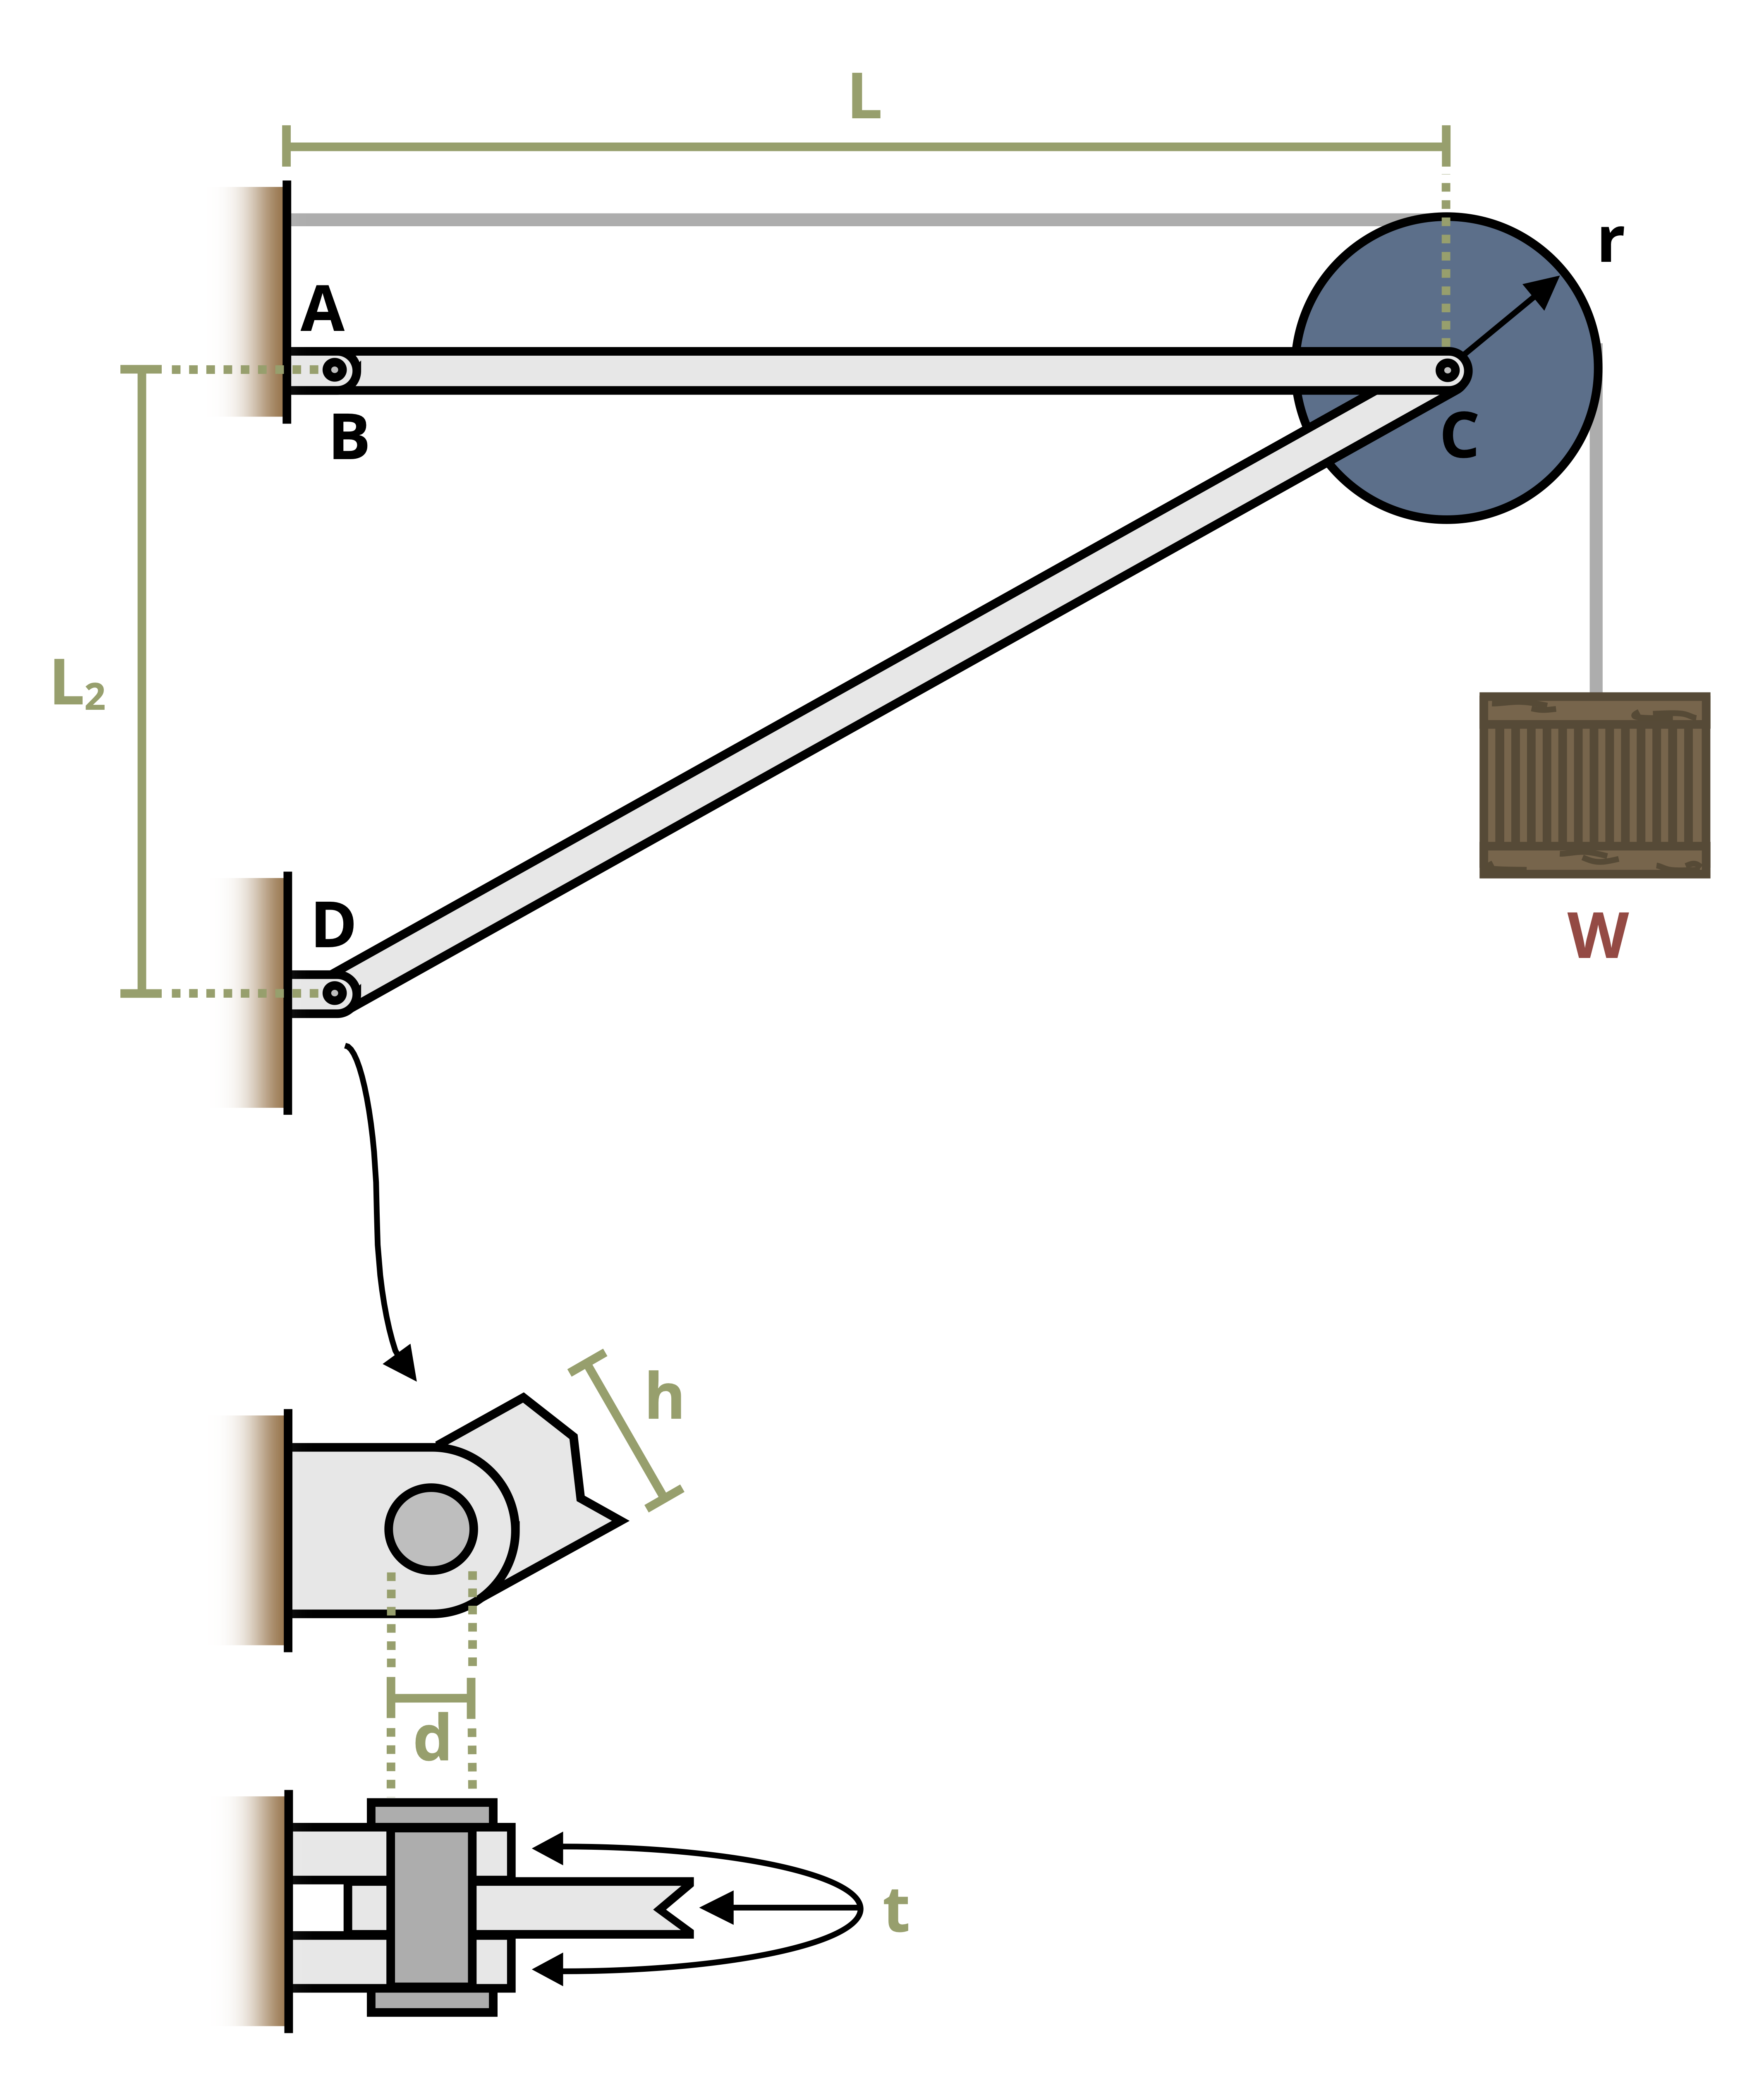
\includegraphics{images/161.png}

}

\caption{Figure 1: A crate is supported by a structure as shown.}

\end{figure}%

\begin{Shaded}
\begin{Highlighting}[]
\NormalTok{\#| standalone: true}
\NormalTok{\#| viewerHeight: 600}
\NormalTok{\#| components: [viewer]}

\NormalTok{from shiny import App, render, ui, reactive}
\NormalTok{import random}
\NormalTok{import asyncio}
\NormalTok{import io}
\NormalTok{import math}
\NormalTok{import string}
\NormalTok{from datetime import datetime}
\NormalTok{from pathlib import Path}

\NormalTok{def generate\_random\_letters(length):}
\NormalTok{    \# Generate a random string of letters of specified length}
\NormalTok{    return \textquotesingle{}\textquotesingle{}.join(random.choice(string.ascii\_lowercase) for \_ in range(length))}

\NormalTok{problem\_ID="161"}
\NormalTok{W=reactive.Value("\_\_")}
\NormalTok{t=reactive.Value("\_\_")}
\NormalTok{d=reactive.Value("\_\_")}
\NormalTok{h=reactive.Value("\_\_")}
  
\NormalTok{attempts=["Timestamp,Attempt,Answer,Feedback\textbackslash{}n"]}

\NormalTok{app\_ui = ui.page\_fluid(}
\NormalTok{    ui.markdown("**Please enter your ID number from your instructor and click to generate your problem**"),}
\NormalTok{    ui.input\_text("ID","", placeholder="Enter ID Number Here"),}
\NormalTok{    ui.input\_action\_button("generate\_problem", "Generate Problem", class\_="btn{-}primary"),}
\NormalTok{    ui.markdown("**Problem Statement**"),}
\NormalTok{    ui.output\_ui("ui\_problem\_statement"),}
\NormalTok{    ui.input\_text("answer","Your Answer in units of ksi", placeholder="Please enter your answer"),}
\NormalTok{    ui.input\_action\_button("submit", "Submit Answer", class\_="btn{-}primary"),}
\NormalTok{    ui.download\_button("download", "Download File to Submit", class\_="btn{-}success"),}
\NormalTok{)}

\NormalTok{def server(input, output, session):}
\NormalTok{    \# Initialize a counter for attempts}
\NormalTok{    attempt\_counter = reactive.Value(0)}

\NormalTok{    @output}
\NormalTok{    @render.ui}
\NormalTok{    def ui\_problem\_statement():}
\NormalTok{        return[ui.markdown(f"A crate weighing W = \{W()\} kips is supported by the structure as shown. The dimensions shown at point D are h = \{h()\} in., t = \{t()\} in., and pin diameter d = \{d()\} in. Determine the bearing stress at joint D due to the pin on member DC.")]}
    
\NormalTok{    @reactive.Effect}
\NormalTok{    @reactive.event(input.generate\_problem)}
\NormalTok{    def randomize\_vars():}
\NormalTok{        random.seed(input.ID())}
\NormalTok{        W.set(random.randrange(5,100,1))}
\NormalTok{        t.set(random.randrange(25, 75, 1)/100)}
\NormalTok{        d.set(t()*4)}
\NormalTok{        h.set(d()*2)}

\NormalTok{    @reactive.Effect}
\NormalTok{    @reactive.event(input.submit)}
\NormalTok{    def \_():}
\NormalTok{        attempt\_counter.set(attempt\_counter() + 1)  \# Increment the attempt counter on each submission.}
\NormalTok{        theta = 29.05*math.pi/180}
\NormalTok{        FDC = W()/math.sin(theta)}
\NormalTok{        instr= FDC/(d()*t()/2)}
\NormalTok{        if math.isclose(float(input.answer()), instr, rel\_tol=0.01):}
\NormalTok{            check = "*Correct*"}
\NormalTok{            correct\_indicator = "JL"}
\NormalTok{        else:}
\NormalTok{            check = "*Not Correct.*"}
\NormalTok{            correct\_indicator = "JG"}

\NormalTok{        \# Generate random parts for the encoded attempt.}
\NormalTok{        random\_start = generate\_random\_letters(4)}
\NormalTok{        random\_middle = generate\_random\_letters(4)}
\NormalTok{        random\_end = generate\_random\_letters(4)}
\NormalTok{        encoded\_attempt = f"\{random\_start\}\{problem\_ID\}{-}\{random\_middle\}\{attempt\_counter()\}\{correct\_indicator\}{-}\{random\_end\}\{input.ID()\}"}

\NormalTok{        \# Store the most recent encoded attempt in a reactive value so it persists across submissions}
\NormalTok{        session.encoded\_attempt = reactive.Value(encoded\_attempt)}

\NormalTok{        \# Append the attempt data to the attempts list without the encoded attempt}
\NormalTok{        attempts.append(f"\{datetime.now()\}, \{attempt\_counter()\}, \{input.answer()\}, \{check\}\textbackslash{}n")}

\NormalTok{        \# Show feedback to the user.}
\NormalTok{        feedback = ui.markdown(f"Your answer of \{input.answer()\} is \{check\}. For reference in debugging this, the calculated instructor answer is \{instr\}")}
\NormalTok{        m = ui.modal(}
\NormalTok{            feedback,}
\NormalTok{            title="Feedback",}
\NormalTok{            easy\_close=True}
\NormalTok{        )}
\NormalTok{        ui.modal\_show(m)}

\NormalTok{    @session.download(filename=lambda: f"Problem\_Log{-}\{problem\_ID\}{-}\{input.ID()\}.csv")}
\NormalTok{    async def download():}
\NormalTok{        \# Start the CSV with the encoded attempt (without label)}
\NormalTok{        final\_encoded = session.encoded\_attempt() if session.encoded\_attempt is not None else "No attempts"}
\NormalTok{        yield f"\{final\_encoded\}\textbackslash{}n\textbackslash{}n"}
        
\NormalTok{        \# Write the header for the remaining CSV data once}
\NormalTok{        yield "Timestamp,Attempt,Answer,Feedback\textbackslash{}n"}
        
\NormalTok{        \# Write the attempts data, ensure that the header from the attempts list is not written again}
\NormalTok{        for attempt in attempts[1:]:  \# Skip the first element which is the header}
\NormalTok{            await asyncio.sleep(0.25)  \# This delay may not be necessary; adjust as needed}
\NormalTok{            yield attempt}

\NormalTok{\# App installation}
\NormalTok{app = App(app\_ui, server)}
\end{Highlighting}
\end{Shaded}

\chapter*{Problem 2.47}\label{problem-2.47-2}
\addcontentsline{toc}{chapter}{Problem 2.47}

\markboth{Problem 2.47}{Problem 2.47}

This is a dynamic rendering of the problem with dynamic variables based
on the username entered.

\section*{Problem Image}\label{problem-image-30}
\addcontentsline{toc}{section}{Problem Image}

\markright{Problem Image}

\begin{figure}[H]

{\centering 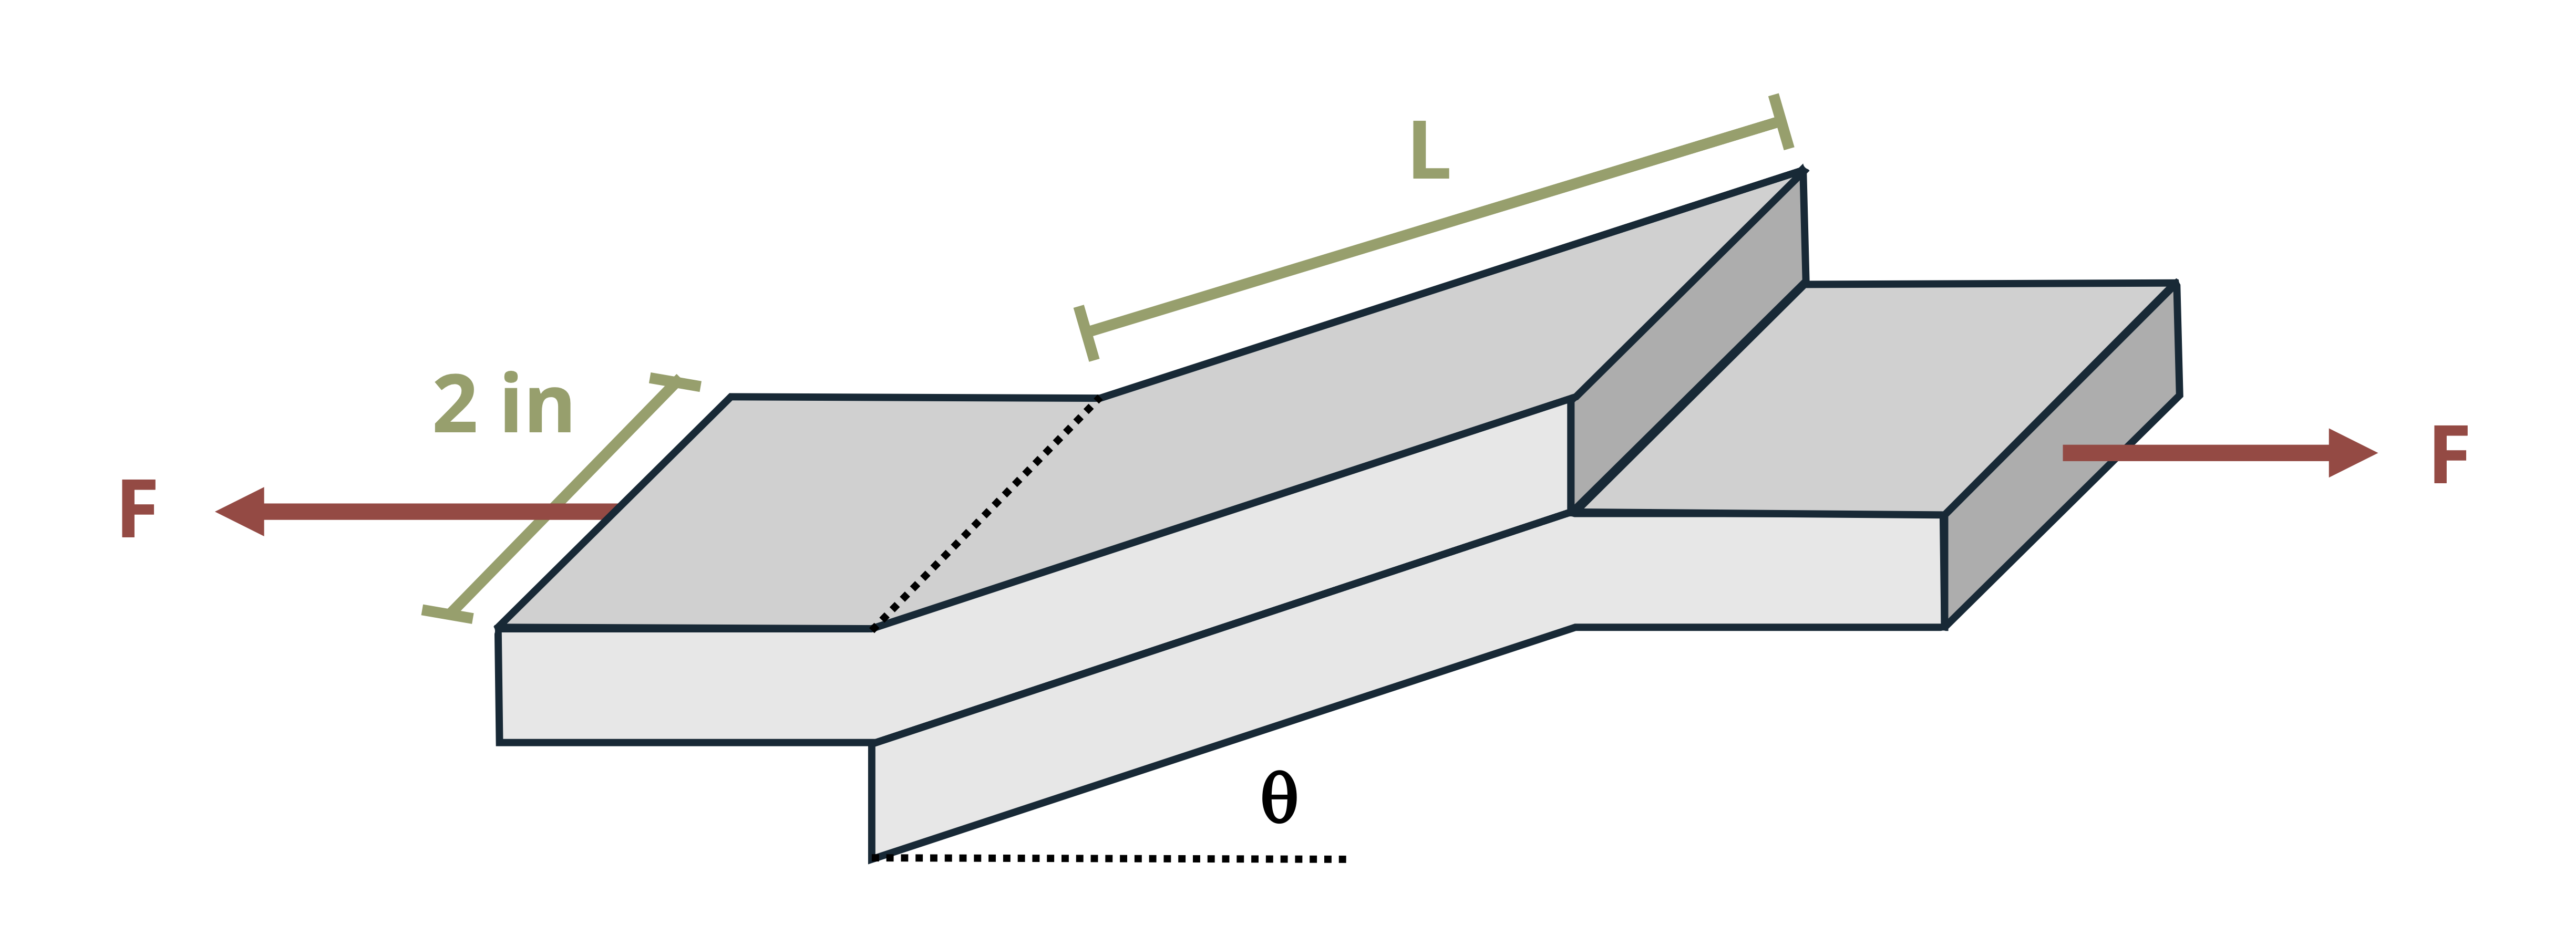
\includegraphics{images/153.png}

}

\caption{Figure 1: Two slanted brackets are glued together.}

\end{figure}%

\begin{Shaded}
\begin{Highlighting}[]
\NormalTok{\#| standalone: true}
\NormalTok{\#| viewerHeight: 600}
\NormalTok{\#| components: [viewer]}

\NormalTok{from shiny import App, render, ui, reactive}
\NormalTok{import random}
\NormalTok{import asyncio}
\NormalTok{import io}
\NormalTok{import math}
\NormalTok{import string}
\NormalTok{from datetime import datetime}
\NormalTok{from pathlib import Path}

\NormalTok{def generate\_random\_letters(length):}
\NormalTok{    \# Generate a random string of letters of specified length}
\NormalTok{    return \textquotesingle{}\textquotesingle{}.join(random.choice(string.ascii\_lowercase) for \_ in range(length))  }

\NormalTok{problem\_ID="153"}
\NormalTok{F=reactive.Value("\_\_")}
\NormalTok{L=reactive.Value("\_\_")}
\NormalTok{Θ=reactive.Value("\_\_")}

\NormalTok{attempts=["Timestamp,Attempt,Answer,Feedback\textbackslash{}n"]}

\NormalTok{app\_ui = ui.page\_fluid(}
\NormalTok{    ui.markdown("**Please enter your ID number from your instructor and click to generate your problem**"),}
\NormalTok{    ui.input\_text("ID","", placeholder="Enter ID Number Here"),}
\NormalTok{    ui.input\_action\_button("generate\_problem", "Generate Problem", class\_="btn{-}primary"),}
\NormalTok{    ui.markdown("**Problem Statement**"),}
\NormalTok{    ui.output\_ui("ui\_problem\_statement"),}
\NormalTok{    ui.input\_text("answer","Your Answer in units of psi", placeholder="Please enter your answer"),}
\NormalTok{    ui.input\_action\_button("submit", "Submit Answer", class\_="btn{-}primary"),}
\NormalTok{    ui.download\_button("download", "Download File to Submit", class\_="btn{-}success"),}
\NormalTok{)}

\NormalTok{def server(input, output, session):}
\NormalTok{    \# Initialize a counter for attempts}
\NormalTok{    attempt\_counter = reactive.Value(0)}

\NormalTok{    @output}
\NormalTok{    @render.ui}
\NormalTok{    def ui\_problem\_statement():}
\NormalTok{        return[ui.markdown(f"Two slanted brackets are glued together as shown. If F = \{F()\} lb, L = \{L()\} in., and Θ = \{Θ()\} °, determine the shear stress parallel to the inclined plane. Assume loads are inline and there is no rotation.")]}
    
\NormalTok{    @reactive.Effect}
\NormalTok{    @reactive.event(input.generate\_problem)}
\NormalTok{    def randomize\_vars():}
\NormalTok{        random.seed(input.ID())}
\NormalTok{        F.set(random.randrange(200, 800, 10))}
\NormalTok{        L.set(random.randrange(20, 80, 1)/10)}
\NormalTok{        Θ.set(random.randrange(15, 30, 1))}
        
\NormalTok{    @reactive.Effect}
\NormalTok{    @reactive.event(input.submit)}
\NormalTok{    def \_():}
\NormalTok{        attempt\_counter.set(attempt\_counter() + 1)  \# Increment the attempt counter on each submission.}
    
\NormalTok{        instr= (F()*math.cos(math.radians(Θ()))/(L()*2))}
\NormalTok{        if math.isclose(float(input.answer()), instr, rel\_tol=0.01):}
\NormalTok{            check = "*Correct*"}
\NormalTok{            correct\_indicator = "JL"}
\NormalTok{        else:}
\NormalTok{            check = "*Not Correct.*"}
\NormalTok{            correct\_indicator = "JG"}

\NormalTok{        \# Generate random parts for the encoded attempt.}
\NormalTok{        random\_start = generate\_random\_letters(4)}
\NormalTok{        random\_middle = generate\_random\_letters(4)}
\NormalTok{        random\_end = generate\_random\_letters(4)}
\NormalTok{        encoded\_attempt = f"\{random\_start\}\{problem\_ID\}{-}\{random\_middle\}\{attempt\_counter()\}\{correct\_indicator\}{-}\{random\_end\}\{input.ID()\}"}

\NormalTok{        \# Store the most recent encoded attempt in a reactive value so it persists across submissions}
\NormalTok{        session.encoded\_attempt = reactive.Value(encoded\_attempt)}

\NormalTok{        \# Append the attempt data to the attempts list without the encoded attempt}
\NormalTok{        attempts.append(f"\{datetime.now()\}, \{attempt\_counter()\}, \{input.answer()\}, \{check\}\textbackslash{}n")}

\NormalTok{        \# Show feedback to the user.}
\NormalTok{        feedback = ui.markdown(f"Your answer of \{input.answer()\} is \{check\}.")}
\NormalTok{        m = ui.modal(}
\NormalTok{            feedback,}
\NormalTok{            title="Feedback",}
\NormalTok{            easy\_close=True}
\NormalTok{        )}
\NormalTok{        ui.modal\_show(m)}

\NormalTok{    @session.download(filename=lambda: f"Problem\_Log{-}\{problem\_ID\}{-}\{input.ID()\}.csv")}
\NormalTok{    async def download():}
\NormalTok{        \# Start the CSV with the encoded attempt (without label)}
\NormalTok{        final\_encoded = session.encoded\_attempt() if session.encoded\_attempt is not None else "No attempts"}
\NormalTok{        yield f"\{final\_encoded\}\textbackslash{}n\textbackslash{}n"}
        
\NormalTok{        \# Write the header for the remaining CSV data once}
\NormalTok{        yield "Timestamp,Attempt,Answer,Feedback\textbackslash{}n"}
        
\NormalTok{        \# Write the attempts data, ensure that the header from the attempts list is not written again}
\NormalTok{        for attempt in attempts[1:]:  \# Skip the first element which is the header}
\NormalTok{            await asyncio.sleep(0.25)  \# This delay may not be necessary; adjust as needed}
\NormalTok{            yield attempt}

\NormalTok{\# App installation}
\NormalTok{app = App(app\_ui, server)}
\end{Highlighting}
\end{Shaded}

\chapter*{Problem 2.48}\label{problem-2.48-2}
\addcontentsline{toc}{chapter}{Problem 2.48}

\markboth{Problem 2.48}{Problem 2.48}

This is a dynamic rendering of the problem with dynamic variables based
on the username entered.

\section*{Problem Image}\label{problem-image-31}
\addcontentsline{toc}{section}{Problem Image}

\markright{Problem Image}

\begin{figure}[H]

{\centering 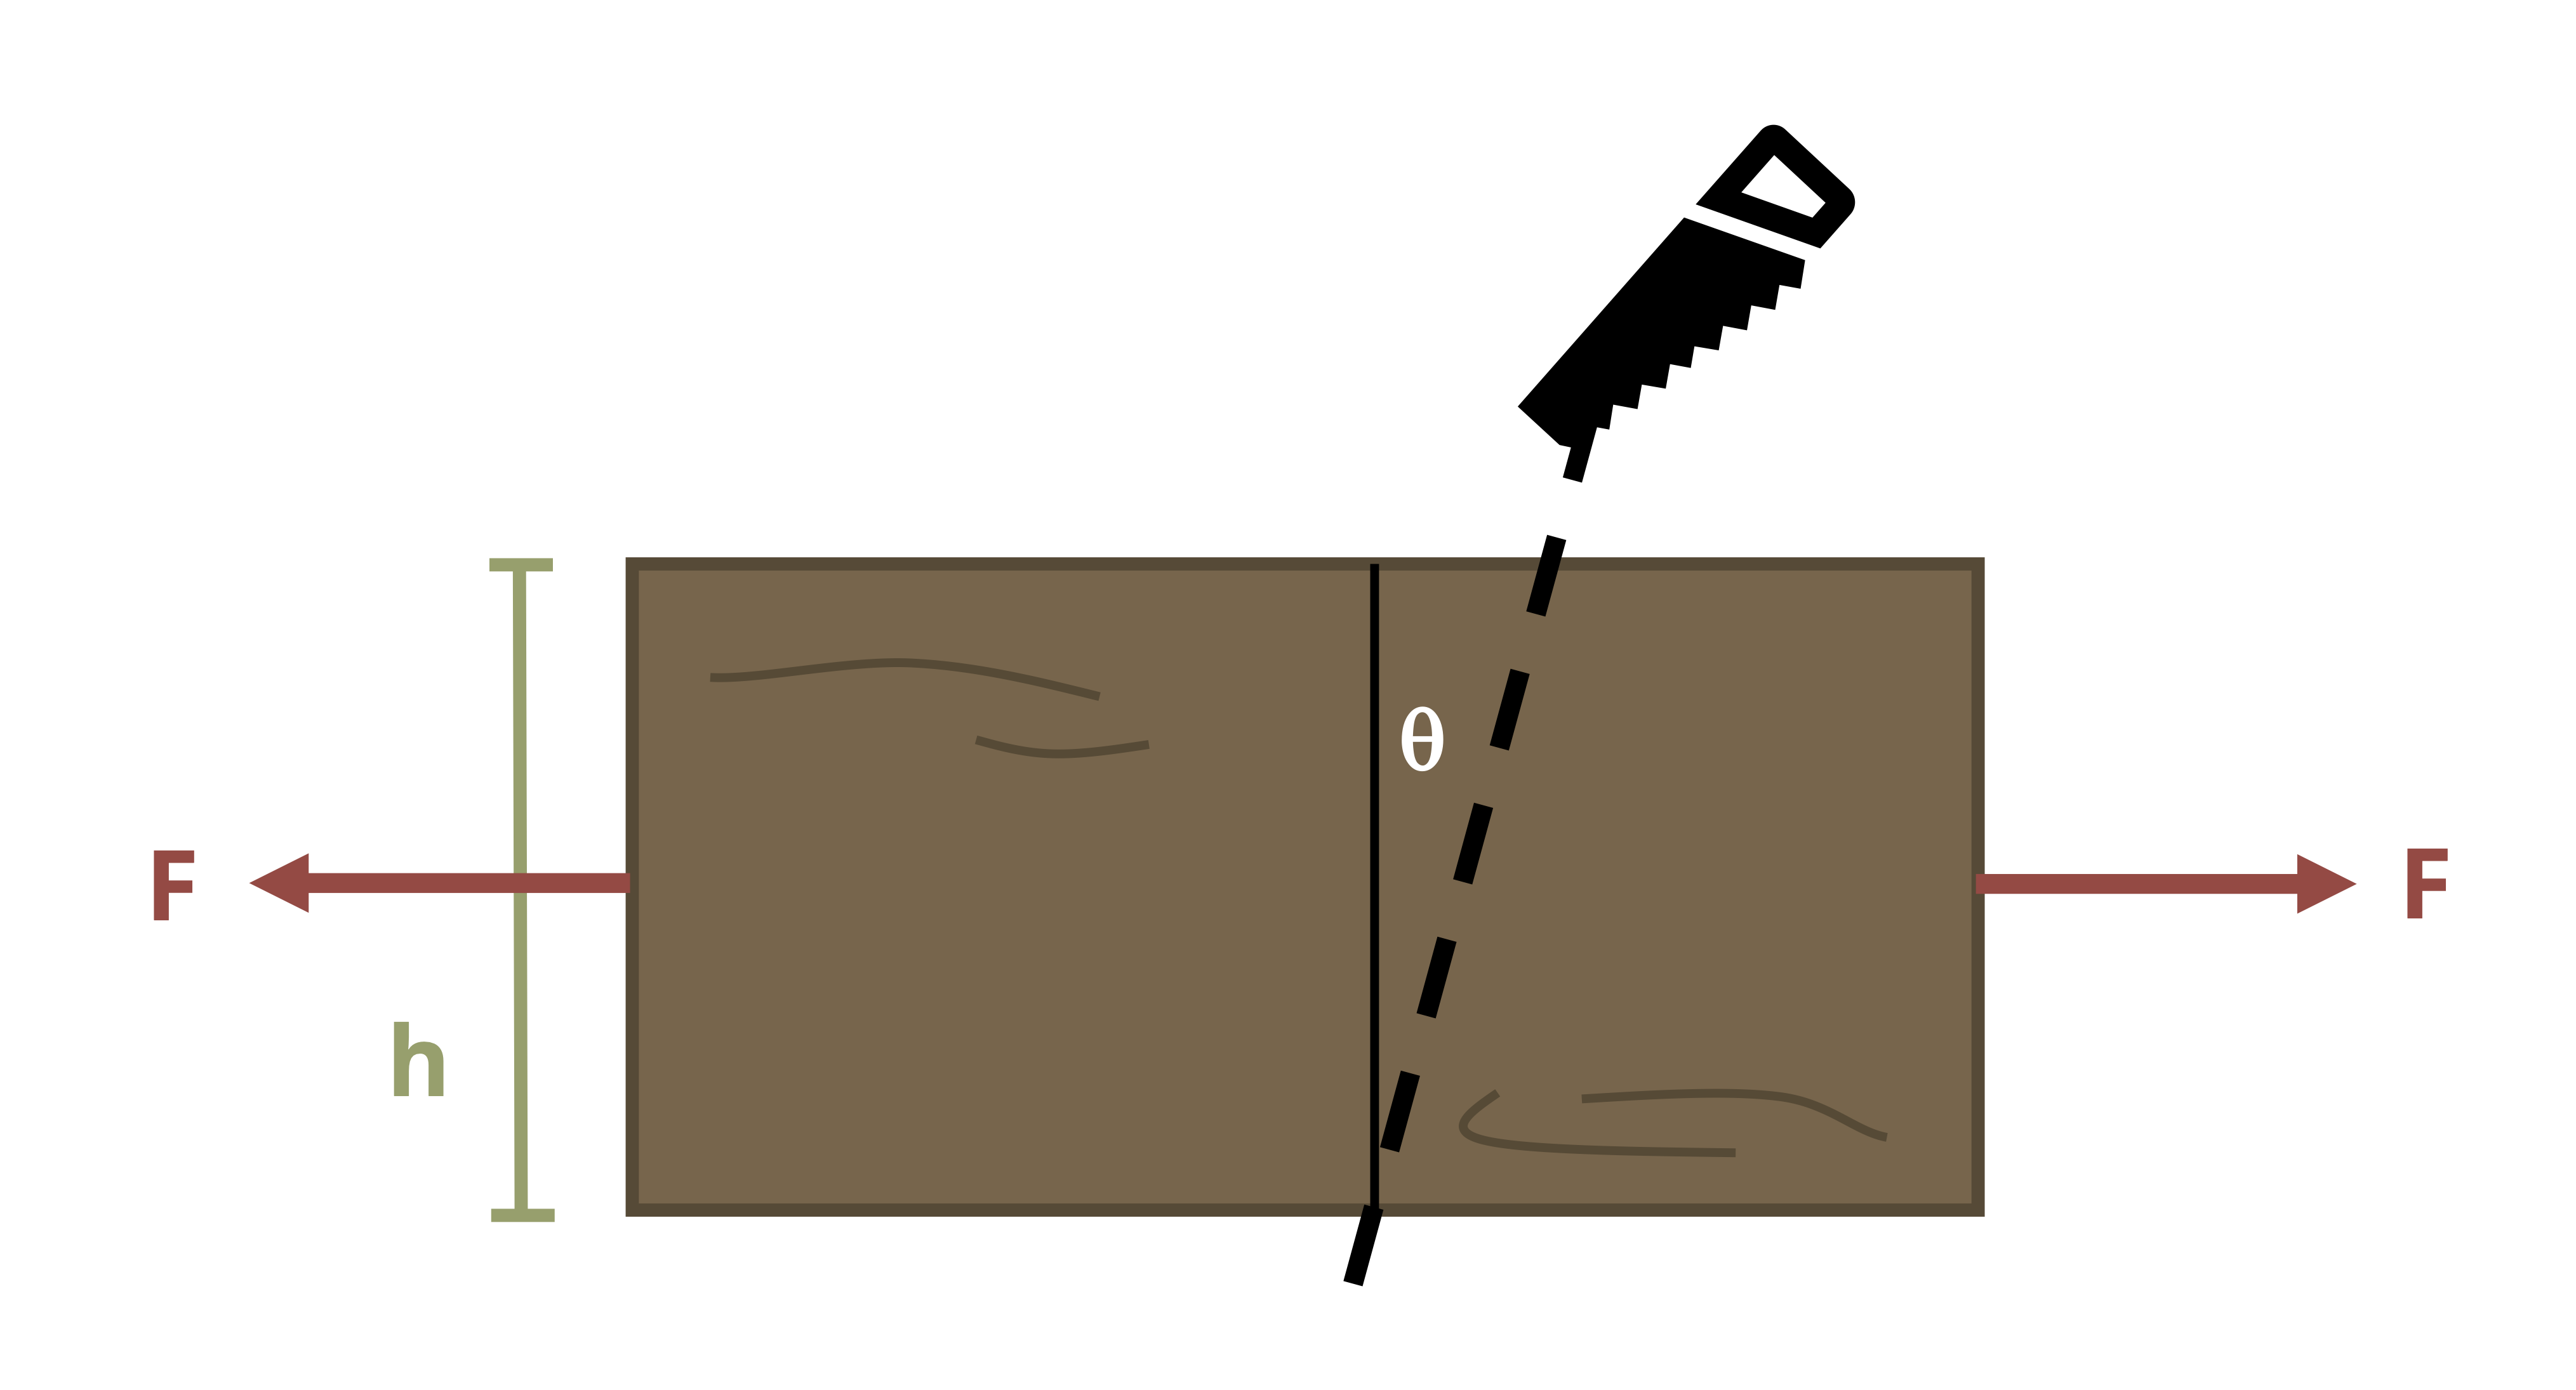
\includegraphics{images/156.png}

}

\caption{Figure 1: A two inch thick board is cut and then glued back
together.}

\end{figure}%

\begin{Shaded}
\begin{Highlighting}[]
\NormalTok{\#| standalone: true}
\NormalTok{\#| viewerHeight: 600}
\NormalTok{\#| components: [viewer]}

\NormalTok{from shiny import App, render, ui, reactive}
\NormalTok{import random}
\NormalTok{import asyncio}
\NormalTok{import io}
\NormalTok{import math}
\NormalTok{import string}
\NormalTok{from datetime import datetime}
\NormalTok{from pathlib import Path}

\NormalTok{def generate\_random\_letters(length):}
\NormalTok{    \# Generate a random string of letters of specified length}
\NormalTok{    return \textquotesingle{}\textquotesingle{}.join(random.choice(string.ascii\_lowercase) for \_ in range(length))  }

\NormalTok{problem\_ID="156"}
\NormalTok{F=reactive.Value("\_\_")}
\NormalTok{h=reactive.Value("\_\_")}
\NormalTok{Θ=reactive.Value("\_\_")}

\NormalTok{attempts=["Timestamp,Attempt,Answer,Feedback\textbackslash{}n"]}

\NormalTok{app\_ui = ui.page\_fluid(}
\NormalTok{    ui.markdown("**Please enter your ID number from your instructor and click to generate your problem**"),}
\NormalTok{    ui.input\_text("ID","", placeholder="Enter ID Number Here"),}
\NormalTok{    ui.input\_action\_button("generate\_problem", "Generate Problem", class\_="btn{-}primary"),}
\NormalTok{    ui.markdown("**Problem Statement**"),}
\NormalTok{    ui.output\_ui("ui\_problem\_statement"),}
\NormalTok{    ui.input\_text("answer","Your Answer in units of psi", placeholder="Please enter your answer"),}
\NormalTok{    ui.input\_action\_button("submit", "Submit Answer", class\_="btn{-}primary"),}
\NormalTok{    ui.download\_button("download", "Download File to Submit", class\_="btn{-}success"),}
\NormalTok{)}


\NormalTok{def server(input, output, session):}
\NormalTok{    \# Initialize a counter for attempts}
\NormalTok{    attempt\_counter = reactive.Value(0)}

\NormalTok{    @output}
\NormalTok{    @render.ui}
\NormalTok{    def ui\_problem\_statement():}
\NormalTok{        return[ui.markdown(f"A 2 inch thick board is cut and then glued back together along a line that is Θ = \{Θ()\} ° off the vertical as shown. If height h = \{h()\} in. and F = \{F()\} lb, determine the normal stress along the cut line.")]}
    
\NormalTok{    @reactive.Effect}
\NormalTok{    @reactive.event(input.generate\_problem)}
\NormalTok{    def randomize\_vars():}
\NormalTok{        random.seed(input.ID())}
\NormalTok{        F.set(random.randrange(2000, 6000, 100))}
\NormalTok{        h.set(random.randrange(50, 150, 1)/10)}
\NormalTok{        Θ.set(random.randrange(10, 20, 1))}
        

\NormalTok{    @reactive.Effect}
\NormalTok{    @reactive.event(input.submit)}
\NormalTok{    def \_():}
\NormalTok{        attempt\_counter.set(attempt\_counter() + 1)  \# Increment the attempt counter on each submission.}
        
\NormalTok{        instr= (F()/(2*h()))*(math.cos(math.radians(Θ()))**2)}
\NormalTok{        if math.isclose(float(input.answer()), instr, rel\_tol=0.01):}
\NormalTok{            check = "*Correct*"}
\NormalTok{            correct\_indicator = "JL"}
\NormalTok{        else:}
\NormalTok{            check = "*Not Correct.*"}
\NormalTok{            correct\_indicator = "JG"}

\NormalTok{        \# Generate random parts for the encoded attempt.}
\NormalTok{        random\_start = generate\_random\_letters(4)}
\NormalTok{        random\_middle = generate\_random\_letters(4)}
\NormalTok{        random\_end = generate\_random\_letters(4)}
\NormalTok{        encoded\_attempt = f"\{random\_start\}\{problem\_ID\}{-}\{random\_middle\}\{attempt\_counter()\}\{correct\_indicator\}{-}\{random\_end\}\{input.ID()\}"}

\NormalTok{        \# Store the most recent encoded attempt in a reactive value so it persists across submissions}
\NormalTok{        session.encoded\_attempt = reactive.Value(encoded\_attempt)}

\NormalTok{        \# Append the attempt data to the attempts list without the encoded attempt}
\NormalTok{        attempts.append(f"\{datetime.now()\}, \{attempt\_counter()\}, \{input.answer()\}, \{check\}\textbackslash{}n")}

\NormalTok{        \# Show feedback to the user.}
\NormalTok{        feedback = ui.markdown(f"Your answer of \{input.answer()\} is \{check\}.")}
\NormalTok{        m = ui.modal(}
\NormalTok{            feedback,}
\NormalTok{            title="Feedback",}
\NormalTok{            easy\_close=True}
\NormalTok{        )}
\NormalTok{        ui.modal\_show(m)}

\NormalTok{    @session.download(filename=lambda: f"Problem\_Log{-}\{problem\_ID\}{-}\{input.ID()\}.csv")}
\NormalTok{    async def download():}
\NormalTok{        \# Start the CSV with the encoded attempt (without label)}
\NormalTok{        final\_encoded = session.encoded\_attempt() if session.encoded\_attempt is not None else "No attempts"}
\NormalTok{        yield f"\{final\_encoded\}\textbackslash{}n\textbackslash{}n"}
        
\NormalTok{        \# Write the header for the remaining CSV data once}
\NormalTok{        yield "Timestamp,Attempt,Answer,Feedback\textbackslash{}n"}
        
\NormalTok{        \# Write the attempts data, ensure that the header from the attempts list is not written again}
\NormalTok{        for attempt in attempts[1:]:  \# Skip the first element which is the header}
\NormalTok{            await asyncio.sleep(0.25)  \# This delay may not be necessary; adjust as needed}
\NormalTok{            yield attempt}


\NormalTok{\# App installation}
\NormalTok{app = App(app\_ui, server)}
\end{Highlighting}
\end{Shaded}

\chapter*{Problem 4.5}\label{problem-4.5}
\addcontentsline{toc}{chapter}{Problem 4.5}

\markboth{Problem 4.5}{Problem 4.5}

This is a dynamic rendering of the problem with dynamic variables based
on the username entered.

\section*{Problem Image}\label{problem-image-32}
\addcontentsline{toc}{section}{Problem Image}

\markright{Problem Image}

\begin{figure}[H]

{\centering 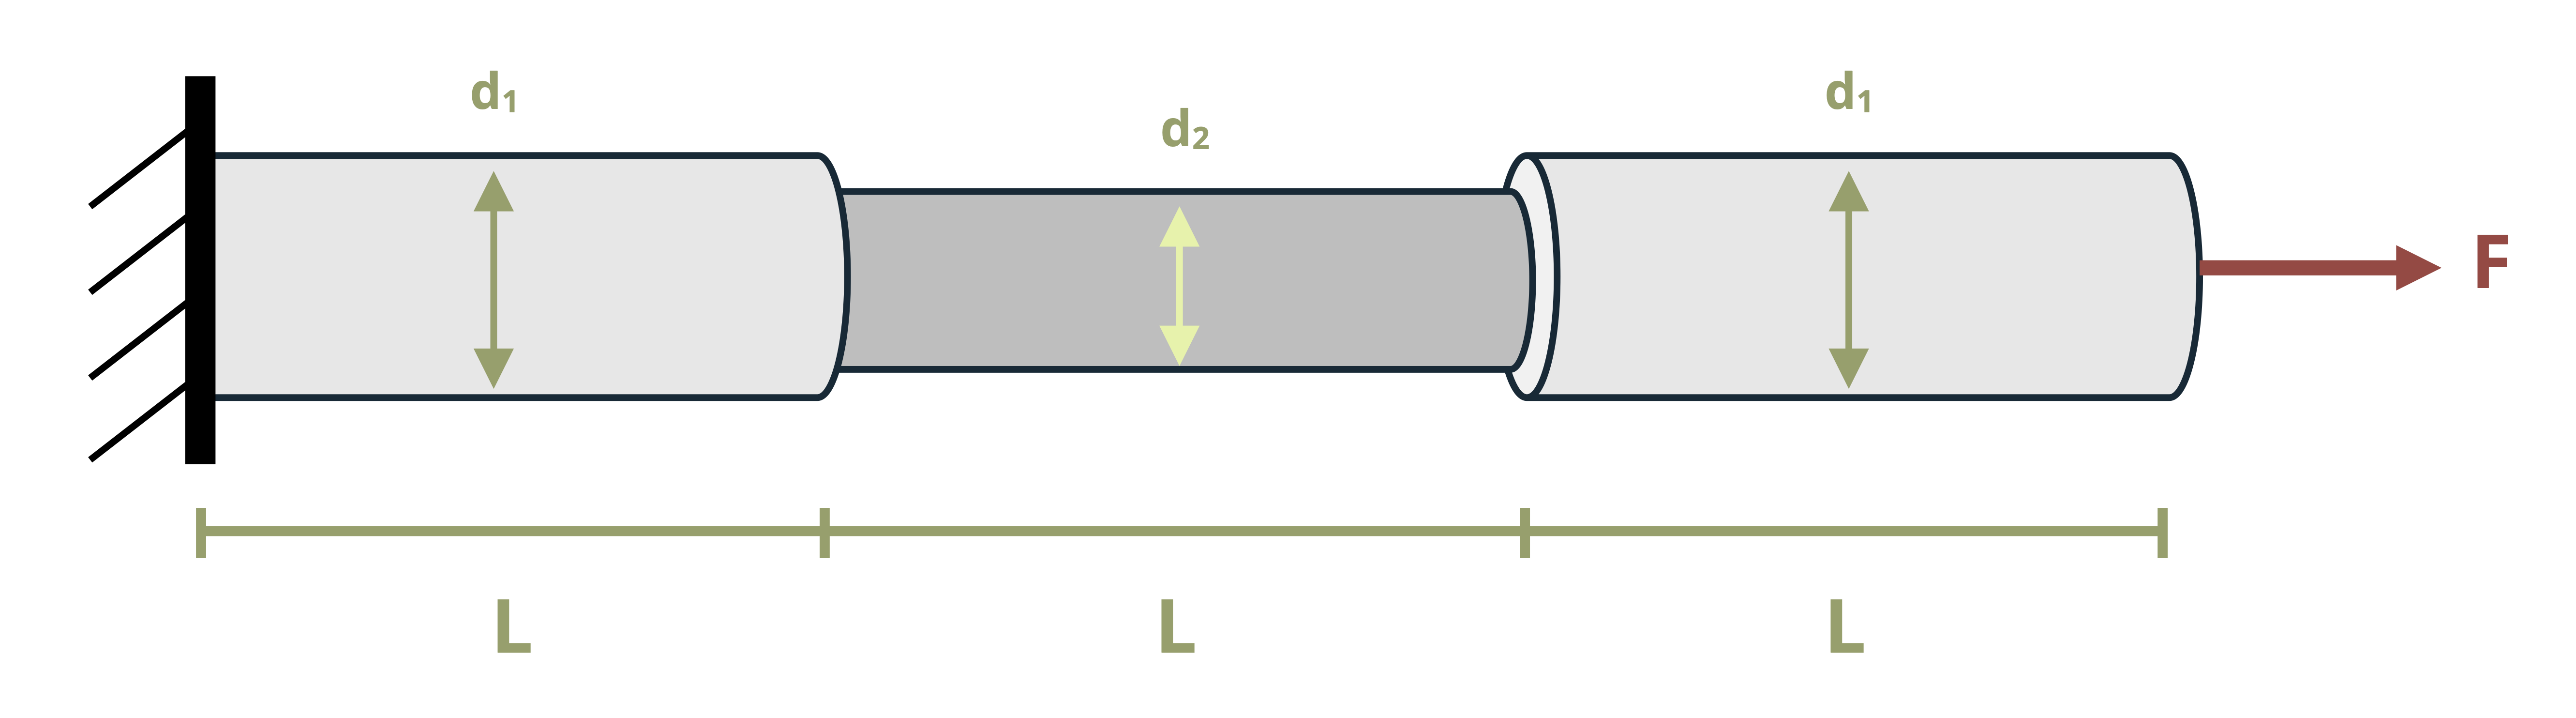
\includegraphics{images/188.png}

}

\caption{Figure 1: A single force pulls on three cylindrical rods that
are fixed to a wall.}

\end{figure}%

\begin{Shaded}
\begin{Highlighting}[]
\NormalTok{\#| standalone: true}
\NormalTok{\#| viewerHeight: 600}
\NormalTok{\#| components: [viewer]}

\NormalTok{from shiny import App, render, ui, reactive}
\NormalTok{import random}
\NormalTok{import asyncio}
\NormalTok{import io}
\NormalTok{import math}
\NormalTok{import string}
\NormalTok{from datetime import datetime}
\NormalTok{from pathlib import Path}

\NormalTok{def generate\_random\_letters(length):}
\NormalTok{    \# Generate a random string of letters of specified length}
\NormalTok{    return \textquotesingle{}\textquotesingle{}.join(random.choice(string.ascii\_lowercase) for \_ in range(length))}

\NormalTok{problem\_ID="188"}
\NormalTok{F=reactive.Value("\_\_")}
\NormalTok{L=reactive.Value("\_\_")}
\NormalTok{d1=reactive.Value("\_\_")}
\NormalTok{d2=reactive.Value("\_\_")}
\NormalTok{Esteel = 29000}
\NormalTok{Ealuminum = 10000}


\NormalTok{attempts=["Timestamp,Attempt,Answer,Feedback\textbackslash{}n"]}

\NormalTok{app\_ui = ui.page\_fluid(}
\NormalTok{    ui.markdown("**Please enter your ID number from your instructor and click to generate your problem**"),}
\NormalTok{    ui.input\_text("ID","", placeholder="Enter ID Number Here"),}
\NormalTok{    ui.input\_action\_button("generate\_problem", "Generate Problem", class\_="btn{-}primary"),}
\NormalTok{    ui.markdown("**Problem Statement**"),}
\NormalTok{    ui.output\_ui("ui\_problem\_statement"),}
\NormalTok{    ui.input\_text("answer","Your Answer in units of inches/inches", placeholder="Please enter your answer"),}
\NormalTok{    ui.input\_action\_button("submit", "Submit Answer", class\_="btn{-}primary"),}
\NormalTok{    ui.download\_button("download", "Download File to Submit", class\_="btn{-}success"),}
\NormalTok{)}


\NormalTok{def server(input, output, session):}
\NormalTok{    \# Initialize a counter for attempts}
\NormalTok{    attempt\_counter = reactive.Value(0)}

\NormalTok{    @output}
\NormalTok{    @render.ui}
\NormalTok{    def ui\_problem\_statement():}
\NormalTok{        return[ui.markdown(f"A single force F = \{F()\} kips pulls on three cylindrical rods, each of length L = \{L()\} in., Diameter d\textless{}sub\textgreater{}1\textless{}/sub\textgreater{} = \{d1()\} in., and d\textless{}sub\textgreater{}2\textless{}/sub\textgreater{} = \{d2()\} in. What is the strain in the steel cylinder? Assume E\textless{}sub\textgreater{}steel\textless{}/sub\textgreater{} = 29,000 ksi and E\textless{}sub\textgreater{}aluminum\textless{}/sub\textgreater{} = 10,000 ksi.")]}
    
\NormalTok{    @reactive.Effect}
\NormalTok{    @reactive.event(input.generate\_problem)}
\NormalTok{    def randomize\_vars():}
\NormalTok{        random.seed(input.ID())}
\NormalTok{        F.set(random.randrange(20, 300, 1)/10)}
\NormalTok{        L.set(random.randrange(50, 200, 1)/10)}
\NormalTok{        d1.set(random.randrange(10, 50, 1)/10)}
\NormalTok{        d2.set(round(d1()/2, 2))}
        
\NormalTok{    @reactive.Effect}
\NormalTok{    @reactive.event(input.submit)}
\NormalTok{    def \_():}
\NormalTok{        attempt\_counter.set(attempt\_counter() + 1)  \# Increment the attempt counter on each submission.}
\NormalTok{        instr=(F()/(((d2()/2)**2)*math.pi))/Esteel}
\NormalTok{        if math.isclose(float(input.answer()), instr, rel\_tol=0.01):}
\NormalTok{            check = "*Correct*"}
\NormalTok{            correct\_indicator = "JL"}
\NormalTok{        else:}
\NormalTok{            check = "*Not Correct.*"}
\NormalTok{            correct\_indicator = "JG"}

\NormalTok{        \# Generate random parts for the encoded attempt.}
\NormalTok{        random\_start = generate\_random\_letters(4)}
\NormalTok{        random\_middle = generate\_random\_letters(4)}
\NormalTok{        random\_end = generate\_random\_letters(4)}
\NormalTok{        encoded\_attempt = f"\{random\_start\}\{problem\_ID\}{-}\{random\_middle\}\{attempt\_counter()\}\{correct\_indicator\}{-}\{random\_end\}\{input.ID()\}"}

\NormalTok{        \# Store the most recent encoded attempt in a reactive value so it persists across submissions}
\NormalTok{        session.encoded\_attempt = reactive.Value(encoded\_attempt)}

\NormalTok{        \# Append the attempt data to the attempts list without the encoded attempt}
\NormalTok{        attempts.append(f"\{datetime.now()\}, \{attempt\_counter()\}, \{input.answer()\}, \{check\}\textbackslash{}n")}

\NormalTok{        \# Show feedback to the user.}
\NormalTok{        feedback = ui.markdown(f"Your answer of \{input.answer()\} is \{check\}.")}
\NormalTok{        m = ui.modal(}
\NormalTok{            feedback,}
\NormalTok{            title="Feedback",}
\NormalTok{            easy\_close=True}
\NormalTok{        )}
\NormalTok{        ui.modal\_show(m)}

\NormalTok{    @session.download(filename=lambda: f"Problem\_Log{-}\{problem\_ID\}{-}\{input.ID()\}.csv")}
\NormalTok{    async def download():}
\NormalTok{        \# Start the CSV with the encoded attempt (without label)}
\NormalTok{        final\_encoded = session.encoded\_attempt() if session.encoded\_attempt is not None else "No attempts"}
\NormalTok{        yield f"\{final\_encoded\}\textbackslash{}n\textbackslash{}n"}
        
\NormalTok{        \# Write the header for the remaining CSV data once}
\NormalTok{        yield "Timestamp,Attempt,Answer,Feedback\textbackslash{}n"}
        
\NormalTok{        \# Write the attempts data, ensure that the header from the attempts list is not written again}
\NormalTok{        for attempt in attempts[1:]:  \# Skip the first element which is the header}
\NormalTok{            await asyncio.sleep(0.25)  \# This delay may not be necessary; adjust as needed}
\NormalTok{            yield attempt}


\NormalTok{\# App installation}
\NormalTok{app = App(app\_ui, server)}
\end{Highlighting}
\end{Shaded}

\chapter*{Problem 4.6}\label{problem-4.6}
\addcontentsline{toc}{chapter}{Problem 4.6}

\markboth{Problem 4.6}{Problem 4.6}

This is a dynamic rendering of the problem with dynamic variables based
on the username entered.

\section*{Problem Image}\label{problem-image-33}
\addcontentsline{toc}{section}{Problem Image}

\markright{Problem Image}

\begin{figure}[H]

{\centering 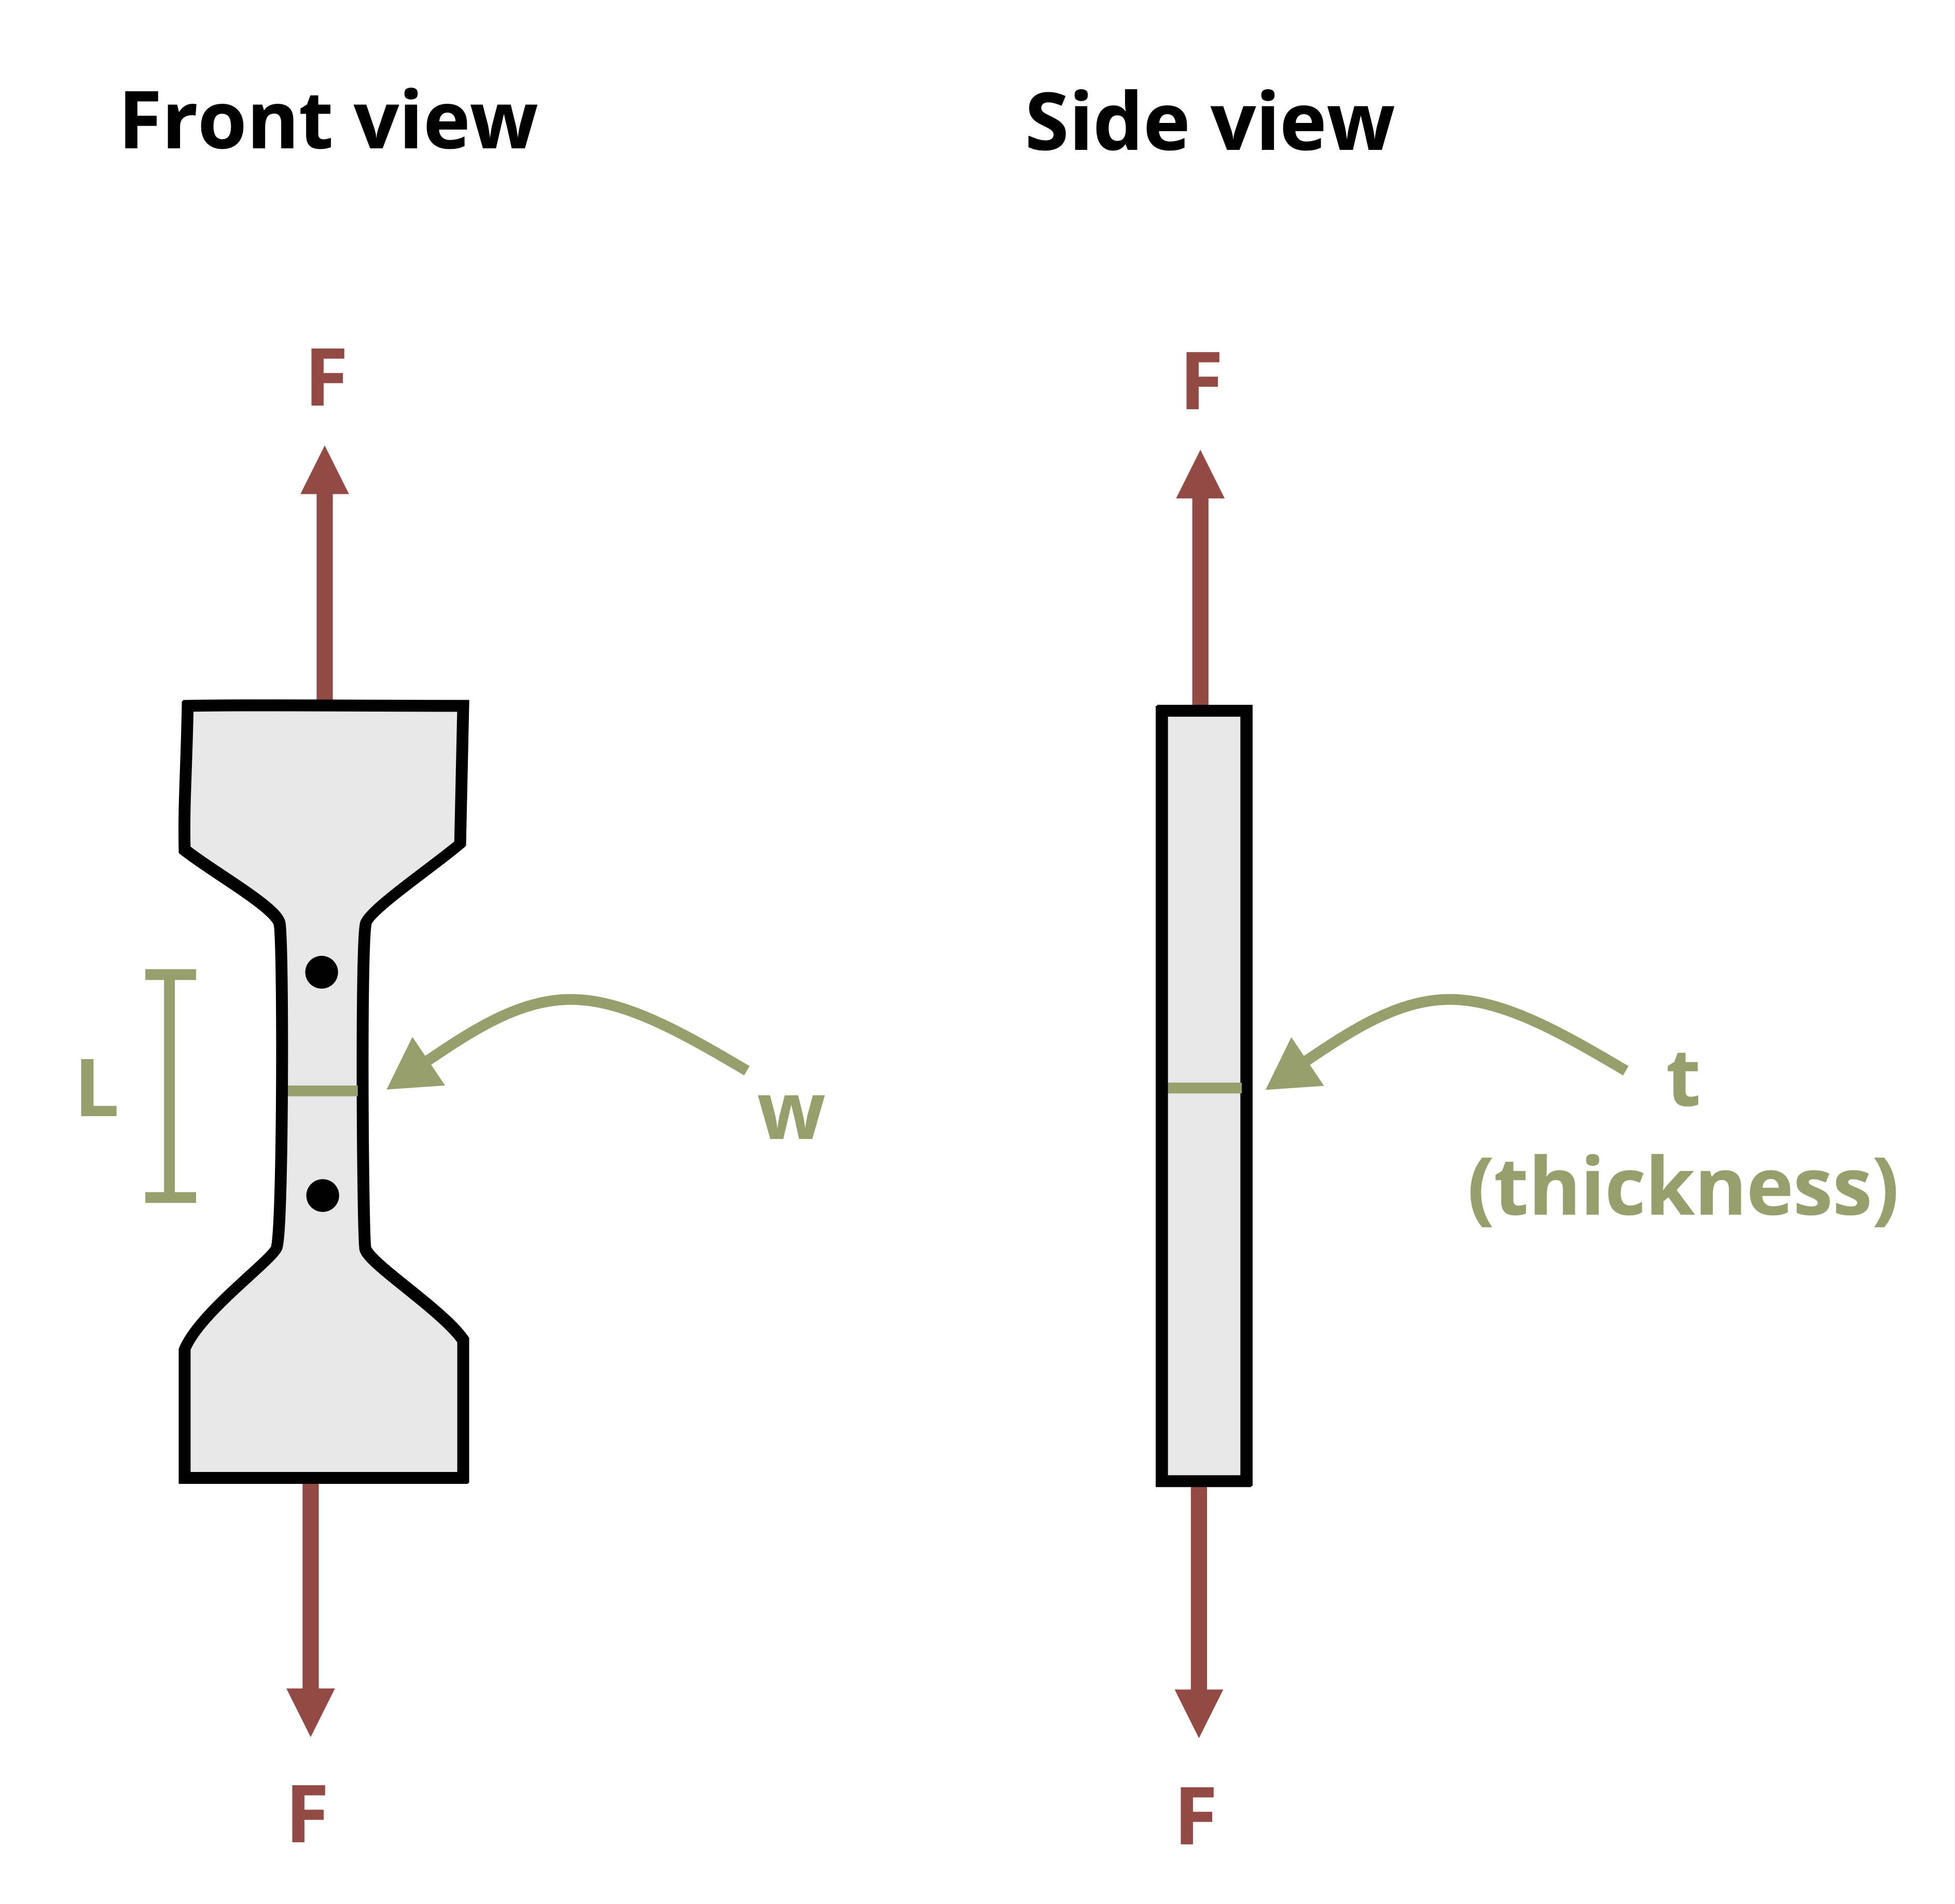
\includegraphics{images/194.png}

}

\caption{Figure 1: A polymer test specimen is pulled from the top and
bottom.}

\end{figure}%

\begin{Shaded}
\begin{Highlighting}[]
\NormalTok{\#| standalone: true}
\NormalTok{\#| viewerHeight: 600}
\NormalTok{\#| components: [viewer]}

\NormalTok{from shiny import App, render, ui, reactive}
\NormalTok{import random}
\NormalTok{import asyncio}
\NormalTok{import io}
\NormalTok{import math}
\NormalTok{import string}
\NormalTok{from datetime import datetime}
\NormalTok{from pathlib import Path}

\NormalTok{def generate\_random\_letters(length):}
\NormalTok{    \# Generate a random string of letters of specified length}
\NormalTok{    return \textquotesingle{}\textquotesingle{}.join(random.choice(string.ascii\_lowercase) for \_ in range(length)) }

\NormalTok{problem\_ID="194"}
\NormalTok{F=reactive.Value("\_\_")}
\NormalTok{L=reactive.Value("\_\_")}
\NormalTok{w=reactive.Value("\_\_")}
\NormalTok{t=reactive.Value("\_\_")}
\NormalTok{dL=reactive.Value("\_\_")}


\NormalTok{attempts=["Timestamp,Attempt,Answer,Feedback\textbackslash{}n"]}

\NormalTok{app\_ui = ui.page\_fluid(}
\NormalTok{    ui.markdown("**Please enter your ID number from your instructor and click to generate your problem**"),}
\NormalTok{    ui.input\_text("ID","", placeholder="Enter ID Number Here"),}
\NormalTok{    ui.input\_action\_button("generate\_problem", "Generate Problem", class\_="btn{-}primary"),}
\NormalTok{    ui.markdown("**Problem Statement**"),}
\NormalTok{    ui.output\_ui("ui\_problem\_statement"),}
\NormalTok{    ui.input\_text("answer","Your Answer in units of ksi", placeholder="Please enter your answer"),}
\NormalTok{    ui.input\_action\_button("submit", "Submit Answer", class\_="btn{-}primary"),}
\NormalTok{    ui.download\_button("download", "Download File to Submit", class\_="btn{-}success"),}
\NormalTok{)}


\NormalTok{def server(input, output, session):}
\NormalTok{    \# Initialize a counter for attempts}
\NormalTok{    attempt\_counter = reactive.Value(0)}

\NormalTok{    @output}
\NormalTok{    @render.ui}
\NormalTok{    def ui\_problem\_statement():}
\NormalTok{        return[ui.markdown(f"A polymer test specimen is subjected to an axial load of F = \{F()\} kips. The central portion of the specimen has an initial length L = \{L()\} in., w = \{w()\} in., and t = \{t()\} in. If the length increases by dL = \{dL()\} in., determine the elastic modulus of the material. ")]}
    
\NormalTok{    @reactive.Effect}
\NormalTok{    @reactive.event(input.generate\_problem)}
\NormalTok{    def randomize\_vars():}
\NormalTok{        random.seed(input.ID())}
\NormalTok{        F.set(random.randrange(100, 500, 1)/10)}
\NormalTok{        L.set(random.randrange(50, 150, 1)/10)}
\NormalTok{        w.set(round(L()*0.375, 2))}
\NormalTok{        t.set(random.randrange(10, 50, 1)/100)}
\NormalTok{        dL.set(random.randrange(3, 9, 1)/100)}
        
\NormalTok{    @reactive.Effect}
\NormalTok{    @reactive.event(input.submit)}
\NormalTok{    def \_():}
\NormalTok{        attempt\_counter.set(attempt\_counter() + 1)  \# Increment the attempt counter on each submission.}
\NormalTok{        instr= (F()*L())/(dL()*(w()*t()))}
\NormalTok{        if math.isclose(float(input.answer()), instr, rel\_tol=0.01):}
\NormalTok{            check = "*Correct*"}
\NormalTok{            correct\_indicator = "JL"}
\NormalTok{        else:}
\NormalTok{            check = "*Not Correct.*"}
\NormalTok{            correct\_indicator = "JG"}

\NormalTok{        \# Generate random parts for the encoded attempt.}
\NormalTok{        random\_start = generate\_random\_letters(4)}
\NormalTok{        random\_middle = generate\_random\_letters(4)}
\NormalTok{        random\_end = generate\_random\_letters(4)}
\NormalTok{        encoded\_attempt = f"\{random\_start\}\{problem\_ID\}{-}\{random\_middle\}\{attempt\_counter()\}\{correct\_indicator\}{-}\{random\_end\}\{input.ID()\}"}

\NormalTok{        \# Store the most recent encoded attempt in a reactive value so it persists across submissions}
\NormalTok{        session.encoded\_attempt = reactive.Value(encoded\_attempt)}

\NormalTok{        \# Append the attempt data to the attempts list without the encoded attempt}
\NormalTok{        attempts.append(f"\{datetime.now()\}, \{attempt\_counter()\}, \{input.answer()\}, \{check\}\textbackslash{}n")}

\NormalTok{        \# Show feedback to the user.}
\NormalTok{        feedback = ui.markdown(f"Your answer of \{input.answer()\} is \{check\}.")}
\NormalTok{        m = ui.modal(}
\NormalTok{            feedback,}
\NormalTok{            title="Feedback",}
\NormalTok{            easy\_close=True}
\NormalTok{        )}
\NormalTok{        ui.modal\_show(m)}

\NormalTok{    @session.download(filename=lambda: f"Problem\_Log{-}\{problem\_ID\}{-}\{input.ID()\}.csv")}
\NormalTok{    async def download():}
\NormalTok{        \# Start the CSV with the encoded attempt (without label)}
\NormalTok{        final\_encoded = session.encoded\_attempt() if session.encoded\_attempt is not None else "No attempts"}
\NormalTok{        yield f"\{final\_encoded\}\textbackslash{}n\textbackslash{}n"}
        
\NormalTok{        \# Write the header for the remaining CSV data once}
\NormalTok{        yield "Timestamp,Attempt,Answer,Feedback\textbackslash{}n"}
        
\NormalTok{        \# Write the attempts data, ensure that the header from the attempts list is not written again}
\NormalTok{        for attempt in attempts[1:]:  \# Skip the first element which is the header}
\NormalTok{            await asyncio.sleep(0.25)  \# This delay may not be necessary; adjust as needed}
\NormalTok{            yield attempt}


\NormalTok{\# App installation}
\NormalTok{app = App(app\_ui, server)}
\end{Highlighting}
\end{Shaded}

\chapter*{Problem 4.10}\label{problem-4.10}
\addcontentsline{toc}{chapter}{Problem 4.10}

\markboth{Problem 4.10}{Problem 4.10}

This is a dynamic rendering of the problem with dynamic variables based
on the username entered.

\section*{Problem Image}\label{problem-image-34}
\addcontentsline{toc}{section}{Problem Image}

\markright{Problem Image}

\begin{figure}[H]

{\centering 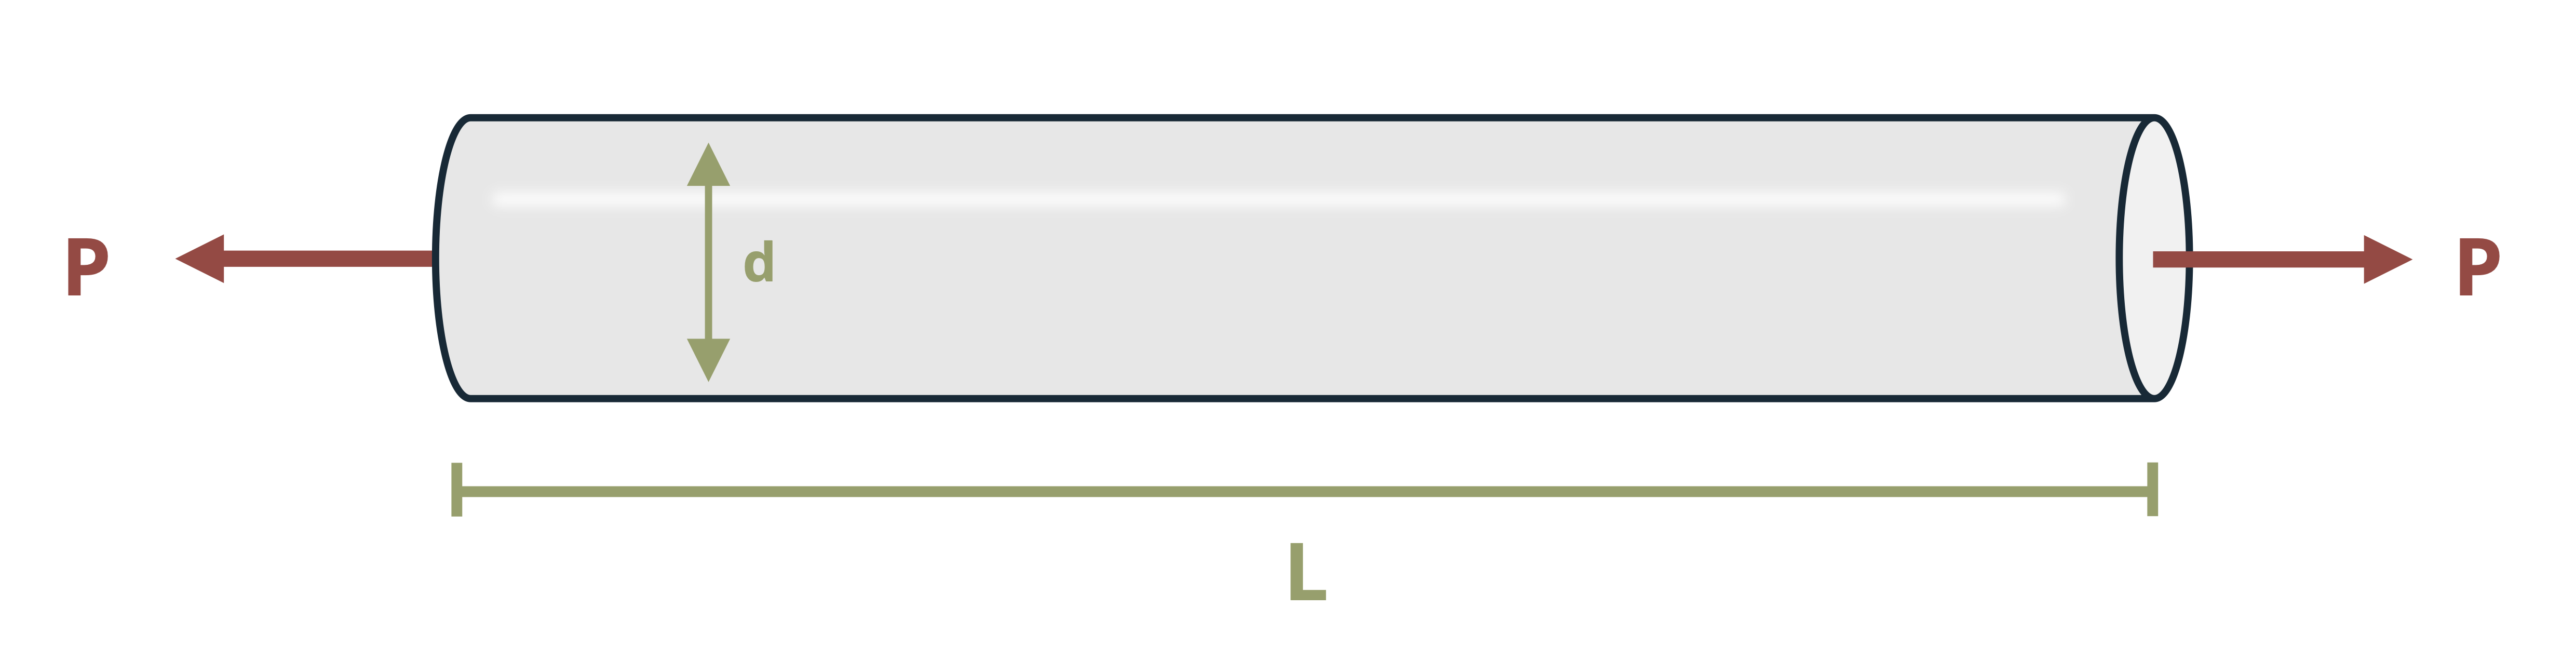
\includegraphics{images/206.png}

}

\caption{Figure 1: A circular road is placed in tension with an axial
load.}

\end{figure}%

\begin{Shaded}
\begin{Highlighting}[]
\NormalTok{\#| standalone: true}
\NormalTok{\#| viewerHeight: 600}
\NormalTok{\#| components: [viewer]}

\NormalTok{from shiny import App, render, ui, reactive}
\NormalTok{import random}
\NormalTok{import asyncio}
\NormalTok{import io}
\NormalTok{import math}
\NormalTok{import string}
\NormalTok{from datetime import datetime}
\NormalTok{from pathlib import Path}

\NormalTok{def generate\_random\_letters(length):}
\NormalTok{    \# Generate a random string of letters of specified length}
\NormalTok{    return \textquotesingle{}\textquotesingle{}.join(random.choice(string.ascii\_lowercase) for \_ in range(length)) }

\NormalTok{problem\_ID="206"}
\NormalTok{P=reactive.Value("\_\_")}
\NormalTok{E=reactive.Value("\_\_")}
\NormalTok{L=reactive.Value("\_\_")}
\NormalTok{d=reactive.Value("\_\_")}

\NormalTok{attempts=["Timestamp,Attempt,Answer,Feedback\textbackslash{}n"]}

\NormalTok{app\_ui = ui.page\_fluid(}
\NormalTok{    ui.markdown("**Please enter your ID number from your instructor and click to generate your problem**"),}
\NormalTok{    ui.input\_text("ID","", placeholder="Enter ID Number Here"),}
\NormalTok{    ui.input\_action\_button("generate\_problem", "Generate Problem", class\_="btn{-}primary"),}
\NormalTok{    ui.markdown("**Problem Statement**"),}
\NormalTok{    ui.output\_ui("ui\_problem\_statement"),}
\NormalTok{    ui.input\_text("answer","Your Answer", placeholder="Please enter your answer"),}
\NormalTok{    ui.input\_action\_button("submit", "Submit Answer", class\_="btn{-}primary"),}
\NormalTok{    ui.download\_button("download", "Download File to Submit", class\_="btn{-}success"),}
\NormalTok{)}

\NormalTok{def server(input, output, session):}
\NormalTok{    \# Initialize a counter for attempts}
\NormalTok{    attempt\_counter = reactive.Value(0)}

\NormalTok{    @output}
\NormalTok{    @render.ui}
\NormalTok{    def ui\_problem\_statement():}
\NormalTok{        return[ui.markdown(f"A circular rod of an unknown metallic alloy is placed in tension with a P = \{P()\} kip axial load. The length of the rod is L = \{L()\} in. and the diameter is d = \{d()\} in. After applying the load, the rod length increases by 0.0035 in and the diameter decreases by 0.00014 in. What is the Poisson\textquotesingle{}s ratio of the alloy?")]}
    
\NormalTok{    @reactive.Effect}
\NormalTok{    @reactive.event(input.generate\_problem)}
\NormalTok{    def randomize\_vars():}
\NormalTok{        random.seed(input.ID())}
\NormalTok{        P.set(random.randrange(20, 200, 1)/10)}
\NormalTok{        L.set(random.randrange(10, 20, 1))}
\NormalTok{        E.set(random.randrange(20, 40, 1)/100)}
\NormalTok{        d.set(round((.00014*L())/(.0035*E()), 1))}
        
\NormalTok{    @reactive.Effect}
\NormalTok{    @reactive.event(input.submit)}
\NormalTok{    def \_():}
\NormalTok{        attempt\_counter.set(attempt\_counter() + 1)  \# Increment the attempt counter on each submission.}
       
\NormalTok{        instr= {-}({-}.00014/d())/(.0035/L())}
\NormalTok{        if math.isclose(float(input.answer()), instr, rel\_tol=0.01):}
\NormalTok{            check = "*Correct*"}
\NormalTok{            correct\_indicator = "JL"}
\NormalTok{        else:}
\NormalTok{            check = "*Not Correct.*"}
\NormalTok{            correct\_indicator = "JG"}

\NormalTok{        \# Generate random parts for the encoded attempt.}
\NormalTok{        random\_start = generate\_random\_letters(4)}
\NormalTok{        random\_middle = generate\_random\_letters(4)}
\NormalTok{        random\_end = generate\_random\_letters(4)}
\NormalTok{        encoded\_attempt = f"\{random\_start\}\{problem\_ID\}{-}\{random\_middle\}\{attempt\_counter()\}\{correct\_indicator\}{-}\{random\_end\}\{input.ID()\}"}

\NormalTok{        \# Store the most recent encoded attempt in a reactive value so it persists across submissions}
\NormalTok{        session.encoded\_attempt = reactive.Value(encoded\_attempt)}

\NormalTok{        \# Append the attempt data to the attempts list without the encoded attempt}
\NormalTok{        attempts.append(f"\{datetime.now()\}, \{attempt\_counter()\}, \{input.answer()\}, \{check\}\textbackslash{}n")}

\NormalTok{        \# Show feedback to the user.}
\NormalTok{        feedback = ui.markdown(f"Your answer of \{input.answer()\} is \{check\}.")}
\NormalTok{        m = ui.modal(}
\NormalTok{            feedback,}
\NormalTok{            title="Feedback",}
\NormalTok{            easy\_close=True}
\NormalTok{        )}
\NormalTok{        ui.modal\_show(m)}

\NormalTok{    @session.download(filename=lambda: f"Problem\_Log{-}\{problem\_ID\}{-}\{input.ID()\}.csv")}
\NormalTok{    async def download():}
\NormalTok{        \# Start the CSV with the encoded attempt (without label)}
\NormalTok{        final\_encoded = session.encoded\_attempt() if session.encoded\_attempt is not None else "No attempts"}
\NormalTok{        yield f"\{final\_encoded\}\textbackslash{}n\textbackslash{}n"}
        
\NormalTok{        \# Write the header for the remaining CSV data once}
\NormalTok{        yield "Timestamp,Attempt,Answer,Feedback\textbackslash{}n"}
        
\NormalTok{        \# Write the attempts data, ensure that the header from the attempts list is not written again}
\NormalTok{        for attempt in attempts[1:]:  \# Skip the first element which is the header}
\NormalTok{            await asyncio.sleep(0.25)  \# This delay may not be necessary; adjust as needed}
\NormalTok{            yield attempt}

\NormalTok{\# App installation}
\NormalTok{app = App(app\_ui, server)}
\end{Highlighting}
\end{Shaded}

\chapter*{Problem 4.11}\label{problem-4.11}
\addcontentsline{toc}{chapter}{Problem 4.11}

\markboth{Problem 4.11}{Problem 4.11}

This is a dynamic rendering of the problem with dynamic variables based
on the username entered.

\section*{Problem Image}\label{problem-image-35}
\addcontentsline{toc}{section}{Problem Image}

\markright{Problem Image}

\begin{figure}[H]

{\centering 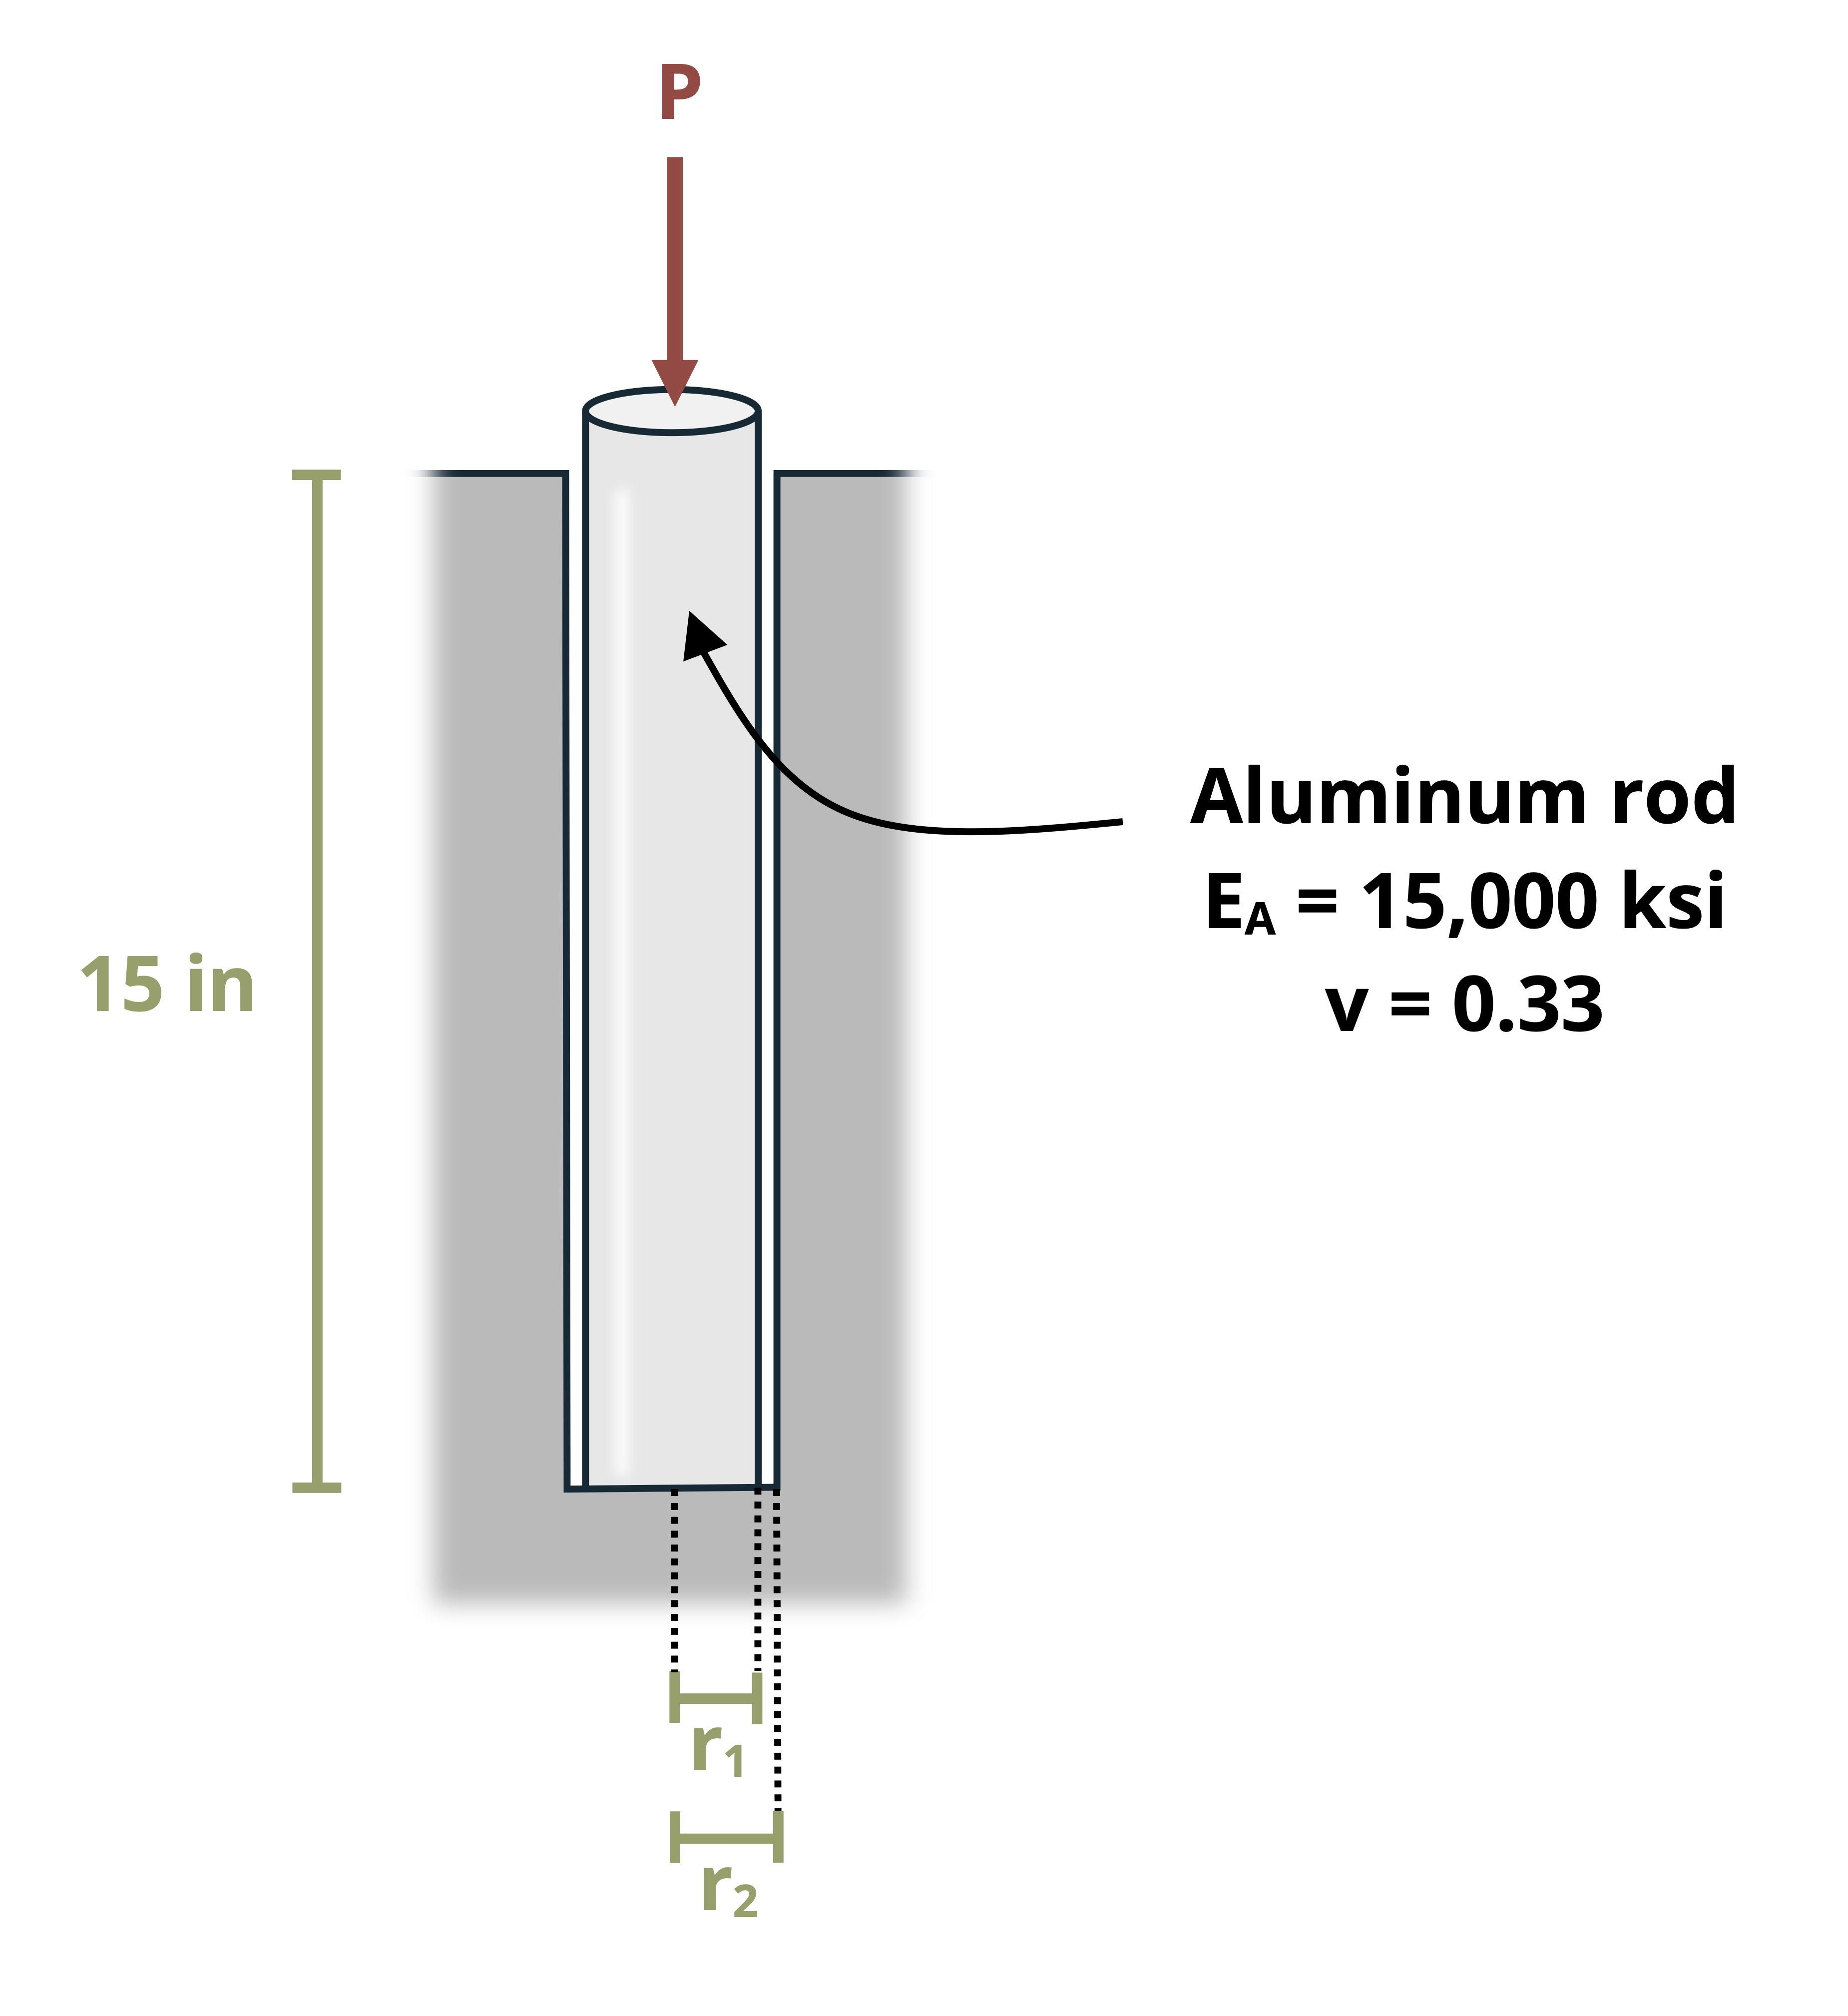
\includegraphics{images/213.png}

}

\caption{Figure 1: A circular rod is inserted into a space slightly
wider than the rod.}

\end{figure}%

\begin{Shaded}
\begin{Highlighting}[]
\NormalTok{\#| standalone: true}
\NormalTok{\#| viewerHeight: 600}
\NormalTok{\#| components: [viewer]}

\NormalTok{from shiny import App, render, ui, reactive}
\NormalTok{import random}
\NormalTok{import asyncio}
\NormalTok{import io}
\NormalTok{import math}
\NormalTok{import string}
\NormalTok{from datetime import datetime}
\NormalTok{from pathlib import Path}

\NormalTok{def generate\_random\_letters(length):}
\NormalTok{    \# Generate a random string of letters of specified length}
\NormalTok{    return \textquotesingle{}\textquotesingle{}.join(random.choice(string.ascii\_lowercase) for \_ in range(length)) }

\NormalTok{problem\_ID="213"}
\NormalTok{r1=reactive.Value("\_\_")}
\NormalTok{r2=reactive.Value("\_\_")}
\NormalTok{E=15000}
\NormalTok{v=0.33}


\NormalTok{attempts=["Timestamp,Attempt,Answer,Feedback\textbackslash{}n"]}

\NormalTok{app\_ui = ui.page\_fluid(}
\NormalTok{    ui.markdown("**Please enter your ID number from your instructor and click to generate your problem**"),}
\NormalTok{    ui.input\_text("ID","", placeholder="Enter ID Number Here"),}
\NormalTok{    ui.input\_action\_button("generate\_problem", "Generate Problem", class\_="btn{-}primary"),}
\NormalTok{    ui.markdown("**Problem Statement**"),}
\NormalTok{    ui.output\_ui("ui\_problem\_statement"),}
\NormalTok{    ui.input\_text("answer","Your Answer in units of kip", placeholder="Please enter your answer"),}
\NormalTok{    ui.input\_action\_button("submit", "Submit Answer", class\_="btn{-}primary"),}
\NormalTok{    ui.download\_button("download", "Download File to Submit", class\_="btn{-}success"),}
\NormalTok{)}


\NormalTok{def server(input, output, session):}
\NormalTok{    \# Initialize a counter for attempts}
\NormalTok{    attempt\_counter = reactive.Value(0)}

\NormalTok{    @output}
\NormalTok{    @render.ui}
\NormalTok{    def ui\_problem\_statement():}
\NormalTok{        return[ui.markdown(f"An aluminum circular rod of radius r\textless{}sub\textgreater{}1\textless{}/sub\textgreater{} = \{r1()\} in is inserted into space that is slightly wider than the rod, where r\textless{}sub\textgreater{}2\textless{}/sub\textgreater{} = \{r2()\} in. What load P is needed so that the rod expands and fills the space in the radial direction? Assume E = 15,000 ksi and v = 0.33. ")]}
    
\NormalTok{    @reactive.Effect}
\NormalTok{    @reactive.event(input.generate\_problem)}
\NormalTok{    def randomize\_vars():}
\NormalTok{        random.seed(input.ID())}
\NormalTok{        r1.set(random.randrange(10, 50, 1)/10)}
\NormalTok{        r2.set((r1() + random.randrange(1, 10, 1)/1000))}
        
\NormalTok{    @reactive.Effect}
\NormalTok{    @reactive.event(input.submit)}
\NormalTok{    def \_():}
\NormalTok{        attempt\_counter.set(attempt\_counter() + 1)  \# Increment the attempt counter on each submission.}
\NormalTok{        Ex = (r1() {-} r2())/r1()}
\NormalTok{        sigmay = (Ex*E)/({-}v)}
\NormalTok{        instr= sigmay*math.pi*r1()**2}
\NormalTok{        if math.isclose(float(input.answer()), instr, rel\_tol=0.01):}
\NormalTok{            check = "*Correct*"}
\NormalTok{            correct\_indicator = "JL"}
\NormalTok{        else:}
\NormalTok{            check = "*Not Correct.*"}
\NormalTok{            correct\_indicator = "JG"}

\NormalTok{        \# Generate random parts for the encoded attempt.}
\NormalTok{        random\_start = generate\_random\_letters(4)}
\NormalTok{        random\_middle = generate\_random\_letters(4)}
\NormalTok{        random\_end = generate\_random\_letters(4)}
\NormalTok{        encoded\_attempt = f"\{random\_start\}\{problem\_ID\}{-}\{random\_middle\}\{attempt\_counter()\}\{correct\_indicator\}{-}\{random\_end\}\{input.ID()\}"}

\NormalTok{        \# Store the most recent encoded attempt in a reactive value so it persists across submissions}
\NormalTok{        session.encoded\_attempt = reactive.Value(encoded\_attempt)}

\NormalTok{        \# Append the attempt data to the attempts list without the encoded attempt}
\NormalTok{        attempts.append(f"\{datetime.now()\}, \{attempt\_counter()\}, \{input.answer()\}, \{check\}\textbackslash{}n")}

\NormalTok{        \# Show feedback to the user.}
\NormalTok{        feedback = ui.markdown(f"Your answer of \{input.answer()\} is \{check\}.")}
\NormalTok{        m = ui.modal(}
\NormalTok{            feedback,}
\NormalTok{            title="Feedback",}
\NormalTok{            easy\_close=True}
\NormalTok{        )}
\NormalTok{        ui.modal\_show(m)}

\NormalTok{    @session.download(filename=lambda: f"Problem\_Log{-}\{problem\_ID\}{-}\{input.ID()\}.csv")}
\NormalTok{    async def download():}
\NormalTok{        \# Start the CSV with the encoded attempt (without label)}
\NormalTok{        final\_encoded = session.encoded\_attempt() if session.encoded\_attempt is not None else "No attempts"}
\NormalTok{        yield f"\{final\_encoded\}\textbackslash{}n\textbackslash{}n"}
        
\NormalTok{        \# Write the header for the remaining CSV data once}
\NormalTok{        yield "Timestamp,Attempt,Answer,Feedback\textbackslash{}n"}
        
\NormalTok{        \# Write the attempts data, ensure that the header from the attempts list is not written again}
\NormalTok{        for attempt in attempts[1:]:  \# Skip the first element which is the header}
\NormalTok{            await asyncio.sleep(0.25)  \# This delay may not be necessary; adjust as needed}
\NormalTok{            yield attempt}


\NormalTok{\# App installation}
\NormalTok{app = App(app\_ui, server)}
\end{Highlighting}
\end{Shaded}

\chapter*{Problem 4.12}\label{problem-4.12}
\addcontentsline{toc}{chapter}{Problem 4.12}

\markboth{Problem 4.12}{Problem 4.12}

This is a dynamic rendering of the problem with dynamic variables based
on the username entered.

\section*{Problem Image}\label{problem-image-36}
\addcontentsline{toc}{section}{Problem Image}

\markright{Problem Image}

\begin{figure}[H]

{\centering 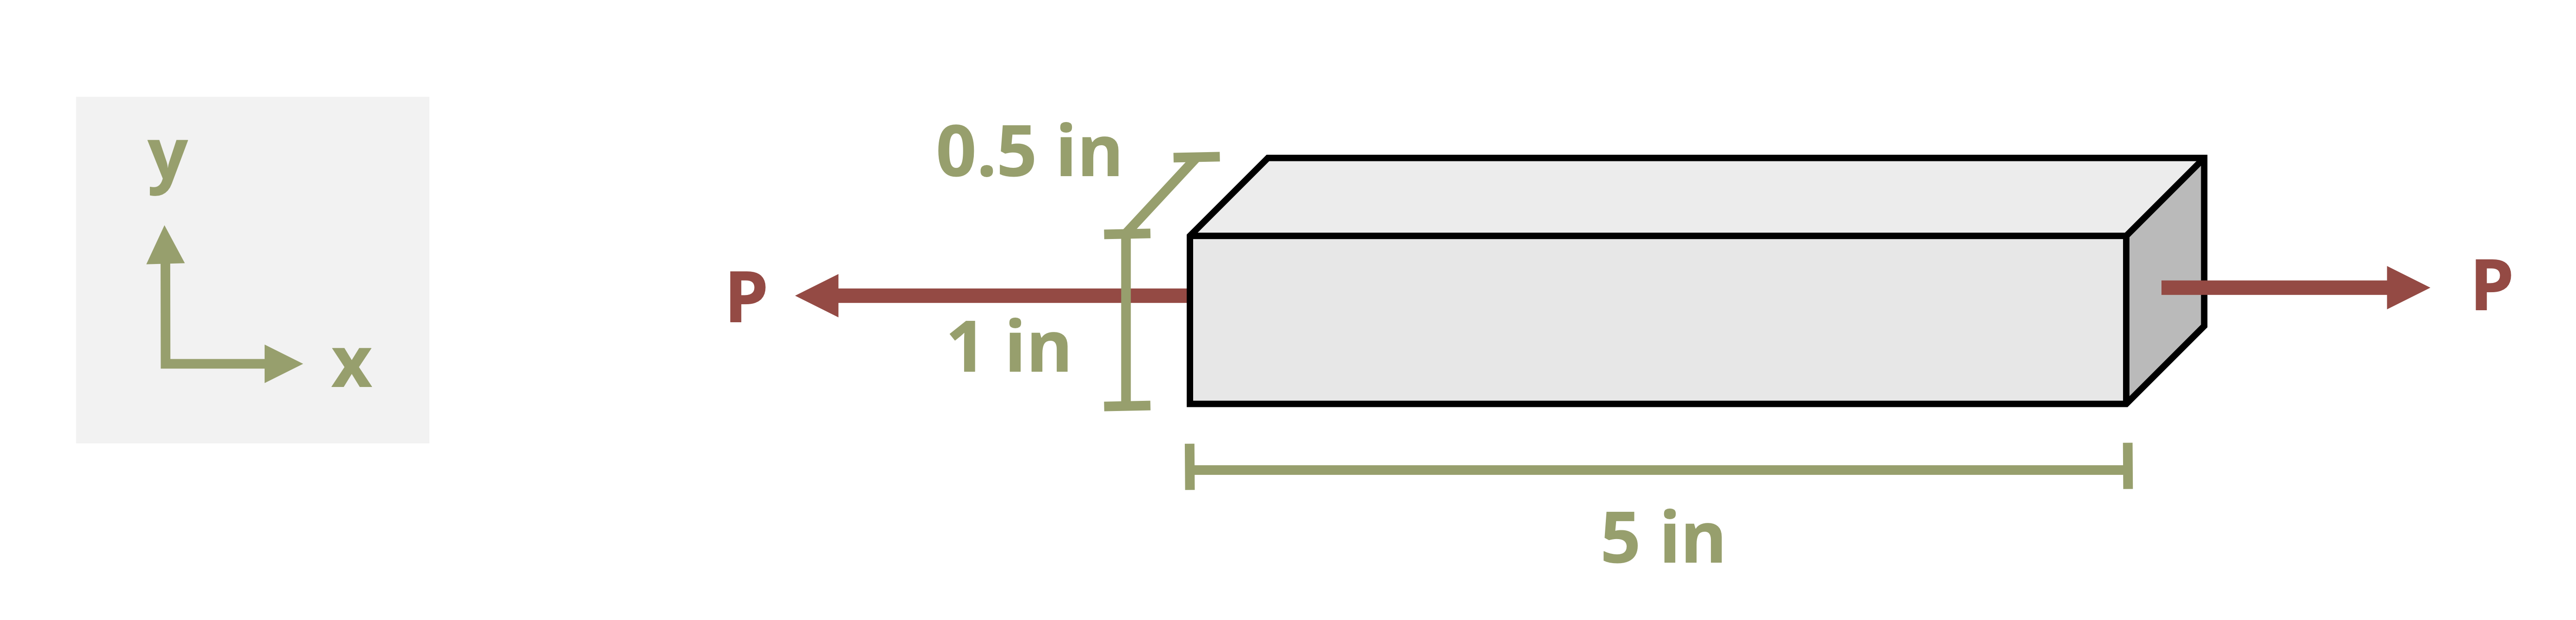
\includegraphics{images/216.png}

}

\caption{Figure 1: A rectangular rod is pulled in tension in the
x-direction.}

\end{figure}%

\begin{Shaded}
\begin{Highlighting}[]
\NormalTok{\#| standalone: true}
\NormalTok{\#| viewerHeight: 600}
\NormalTok{\#| components: [viewer]}

\NormalTok{from shiny import App, render, ui, reactive}
\NormalTok{import random}
\NormalTok{import asyncio}
\NormalTok{import io}
\NormalTok{import math}
\NormalTok{import string}
\NormalTok{from datetime import datetime}
\NormalTok{from pathlib import Path}

\NormalTok{def generate\_random\_letters(length):}
\NormalTok{    \# Generate a random string of letters of specified length}
\NormalTok{    return \textquotesingle{}\textquotesingle{}.join(random.choice(string.ascii\_lowercase) for \_ in range(length)) }

\NormalTok{problem\_ID="216"}
\NormalTok{d1=reactive.Value("\_\_")}
\NormalTok{d2=reactive.Value("\_\_")}


\NormalTok{attempts=["Timestamp,Attempt,Answer,Feedback\textbackslash{}n"]}

\NormalTok{app\_ui = ui.page\_fluid(}
\NormalTok{    ui.markdown("**Please enter your ID number from your instructor and click to generate your problem**"),}
\NormalTok{    ui.input\_text("ID","", placeholder="Enter ID Number Here"),}
\NormalTok{    ui.input\_action\_button("generate\_problem", "Generate Problem", class\_="btn{-}primary"),}
\NormalTok{    ui.markdown("**Problem Statement**"),}
\NormalTok{    ui.output\_ui("ui\_problem\_statement"),}
\NormalTok{    ui.input\_text("answer","Your Answer", placeholder="Please enter your answer"),}
\NormalTok{    ui.input\_action\_button("submit", "Submit Answer", class\_="btn{-}primary"),}
\NormalTok{    ui.download\_button("download", "Download File to Submit", class\_="btn{-}success"),}
\NormalTok{)}


\NormalTok{def server(input, output, session):}
\NormalTok{    \# Initialize a counter for attempts}
\NormalTok{    attempt\_counter = reactive.Value(0)}

\NormalTok{    @output}
\NormalTok{    @render.ui}
\NormalTok{    def ui\_problem\_statement():}
\NormalTok{        return[ui.markdown(f"A rectangular bar is pulled in tension by a load P in the x{-}direction. The bar deflects by d\textless{}sub\textgreater{}1\textless{}/sub\textgreater{} = \{d1()\} in and d\textless{}sub\textgreater{}2\textless{}/sub\textgreater{} = {-} \{d2()\} in, in the x{-} and y{-}direction, respectively. The length in the x{-}direction is 5 in, and the length in the y direction is 1 in. What is the Poisson\textquotesingle{}s ratio of the material? The z{-}direction deflection is not known. ")]}
    
\NormalTok{    @reactive.Effect}
\NormalTok{    @reactive.event(input.generate\_problem)}
\NormalTok{    def randomize\_vars():}
\NormalTok{        random.seed(input.ID())}
\NormalTok{        d1.set(random.randrange(20, 50, 1)/1000)}
\NormalTok{        d2.set(random.randrange(10, 20, 1)/10000)}
        
\NormalTok{    @reactive.Effect}
\NormalTok{    @reactive.event(input.submit)}
\NormalTok{    def \_():}
\NormalTok{        attempt\_counter.set(attempt\_counter() + 1)  \# Increment the attempt counter on each submission.}
\NormalTok{        instr= {-}({-}d2()/1)/(d1()/5)}
\NormalTok{        if math.isclose(float(input.answer()), instr, rel\_tol=0.01):}
\NormalTok{            check = "*Correct*"}
\NormalTok{            correct\_indicator = "JL"}
\NormalTok{        else:}
\NormalTok{            check = "*Not Correct.*"}
\NormalTok{            correct\_indicator = "JG"}

\NormalTok{        \# Generate random parts for the encoded attempt.}
\NormalTok{        random\_start = generate\_random\_letters(4)}
\NormalTok{        random\_middle = generate\_random\_letters(4)}
\NormalTok{        random\_end = generate\_random\_letters(4)}
\NormalTok{        encoded\_attempt = f"\{random\_start\}\{problem\_ID\}{-}\{random\_middle\}\{attempt\_counter()\}\{correct\_indicator\}{-}\{random\_end\}\{input.ID()\}"}

\NormalTok{        \# Store the most recent encoded attempt in a reactive value so it persists across submissions}
\NormalTok{        session.encoded\_attempt = reactive.Value(encoded\_attempt)}

\NormalTok{        \# Append the attempt data to the attempts list without the encoded attempt}
\NormalTok{        attempts.append(f"\{datetime.now()\}, \{attempt\_counter()\}, \{input.answer()\}, \{check\}\textbackslash{}n")}

\NormalTok{        \# Show feedback to the user.}
\NormalTok{        feedback = ui.markdown(f"Your answer of \{input.answer()\} is \{check\}.")}
\NormalTok{        m = ui.modal(}
\NormalTok{            feedback,}
\NormalTok{            title="Feedback",}
\NormalTok{            easy\_close=True}
\NormalTok{        )}
\NormalTok{        ui.modal\_show(m)}

\NormalTok{    @session.download(filename=lambda: f"Problem\_Log{-}\{problem\_ID\}{-}\{input.ID()\}.csv")}
\NormalTok{    async def download():}
\NormalTok{        \# Start the CSV with the encoded attempt (without label)}
\NormalTok{        final\_encoded = session.encoded\_attempt() if session.encoded\_attempt is not None else "No attempts"}
\NormalTok{        yield f"\{final\_encoded\}\textbackslash{}n\textbackslash{}n"}
        
\NormalTok{        \# Write the header for the remaining CSV data once}
\NormalTok{        yield "Timestamp,Attempt,Answer,Feedback\textbackslash{}n"}
        
\NormalTok{        \# Write the attempts data, ensure that the header from the attempts list is not written again}
\NormalTok{        for attempt in attempts[1:]:  \# Skip the first element which is the header}
\NormalTok{            await asyncio.sleep(0.25)  \# This delay may not be necessary; adjust as needed}
\NormalTok{            yield attempt}


\NormalTok{\# App installation}
\NormalTok{app = App(app\_ui, server)}
\end{Highlighting}
\end{Shaded}

\chapter*{Problem 4.23}\label{problem-4.23}
\addcontentsline{toc}{chapter}{Problem 4.23}

\markboth{Problem 4.23}{Problem 4.23}

This is a dynamic rendering of the problem with dynamic variables based
on the username entered.

\section*{Problem Image}\label{problem-image-37}
\addcontentsline{toc}{section}{Problem Image}

\markright{Problem Image}

\begin{figure}[H]

{\centering 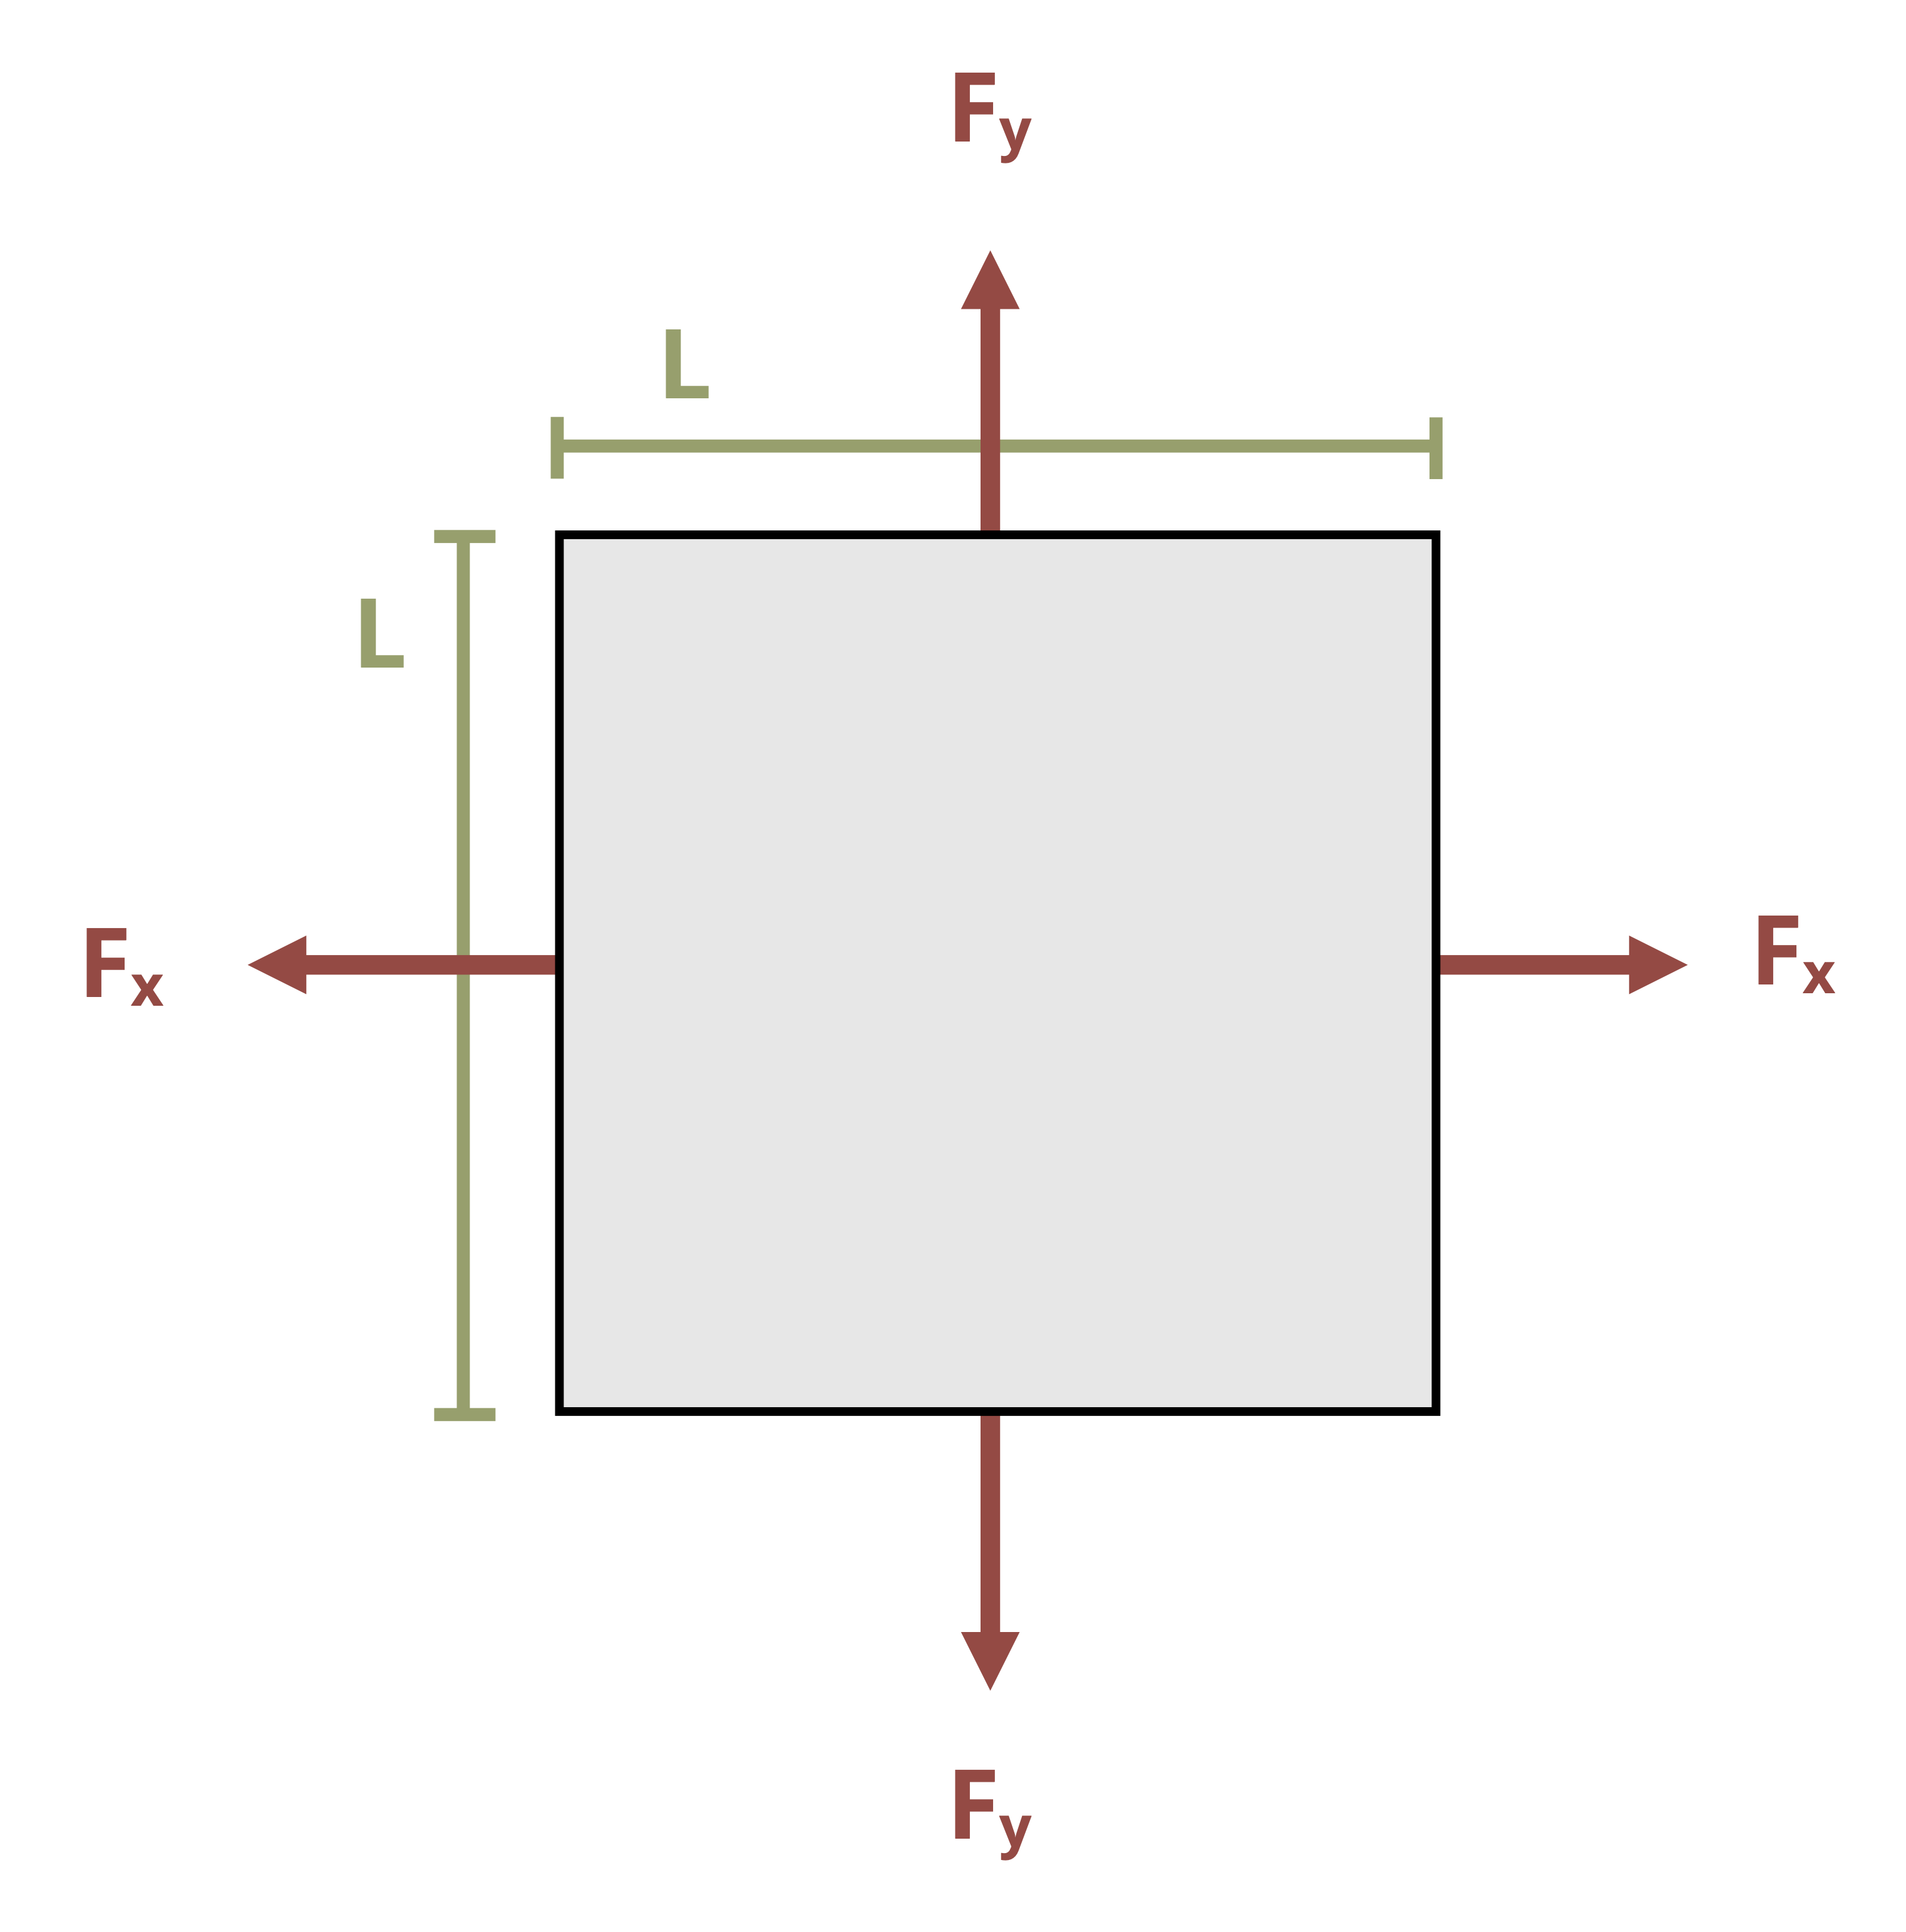
\includegraphics{images/204.png}

}

\caption{Figure 1: A block is pulled in by two forces.}

\end{figure}%

\begin{Shaded}
\begin{Highlighting}[]
\NormalTok{\#| standalone: true}
\NormalTok{\#| viewerHeight: 600}
\NormalTok{\#| components: [viewer]}

\NormalTok{from shiny import App, render, ui, reactive}
\NormalTok{import random}
\NormalTok{import asyncio}
\NormalTok{import io}
\NormalTok{import math}
\NormalTok{import string}
\NormalTok{from datetime import datetime}
\NormalTok{from pathlib import Path}

\NormalTok{def generate\_random\_letters(length):}
\NormalTok{    \# Generate a random string of letters of specified length}
\NormalTok{    return \textquotesingle{}\textquotesingle{}.join(random.choice(string.ascii\_lowercase) for \_ in range(length)) }

\NormalTok{problem\_ID="204"}
\NormalTok{L=reactive.Value("\_\_")}
\NormalTok{t=reactive.Value("\_\_")}
\NormalTok{Fx=reactive.Value("\_\_")}
\NormalTok{Fy=reactive.Value("\_\_")}
\NormalTok{E=29000}
\NormalTok{v=0.29}


\NormalTok{attempts=["Timestamp,Attempt,Answer,Feedback\textbackslash{}n"]}

\NormalTok{app\_ui = ui.page\_fluid(}
\NormalTok{    ui.markdown("**Please enter your ID number from your instructor and click to generate your problem**"),}
\NormalTok{    ui.input\_text("ID","", placeholder="Enter ID Number Here"),}
\NormalTok{    ui.input\_action\_button("generate\_problem", "Generate Problem", class\_="btn{-}primary"),}
\NormalTok{    ui.markdown("**Problem Statement**"),}
\NormalTok{    ui.output\_ui("ui\_problem\_statement"),}
\NormalTok{    ui.input\_text("answer","Your Answer in units of inches", placeholder="Please enter your answer"),}
\NormalTok{    ui.input\_action\_button("submit", "Submit Answer", class\_="btn{-}primary"),}
\NormalTok{    ui.download\_button("download", "Download File to Submit", class\_="btn{-}success"),}
\NormalTok{)}


\NormalTok{def server(input, output, session):}
\NormalTok{    \# Initialize a counter for attempts}
\NormalTok{    attempt\_counter = reactive.Value(0)}

\NormalTok{    @output}
\NormalTok{    @render.ui}
\NormalTok{    def ui\_problem\_statement():}
\NormalTok{        return[ui.markdown(f"A square steel plate of side length L = \{L()\} in. and thickness t = \{t()\} in. is uniformly pulled by two forces F\textless{}sub\textgreater{}x\textless{}/sub\textgreater{} = \{Fx()\} kips and F\textless{}sub\textgreater{}y\textless{}/sub\textgreater{} = \{Fy()\} kips as shown. If E = 29,000 ksi and Poisson\textquotesingle{}s ratio v = 0.29, determine the change in thickness of the plate. ")]}
    
\NormalTok{    @reactive.Effect}
\NormalTok{    @reactive.event(input.generate\_problem)}
\NormalTok{    def randomize\_vars():}
\NormalTok{        random.seed(input.ID())}
\NormalTok{        L.set(random.randrange(50, 150, 1)/10)}
\NormalTok{        t.set(random.randrange(2, 10, 1)/10)}
\NormalTok{        Fx.set(random.randrange(100, 500, 1)/10)}
\NormalTok{        Fy.set(random.randrange(100, 500, 1)/10)}
        
\NormalTok{    @reactive.Effect}
\NormalTok{    @reactive.event(input.submit)}
\NormalTok{    def \_():}
\NormalTok{        attempt\_counter.set(attempt\_counter() + 1)  \# Increment the attempt counter on each submission.}
\NormalTok{        sigmax = Fx()/(L()*t())}
\NormalTok{        sigmay = Fy()/(L()*t())}
\NormalTok{        instr= t()*({-}v/E)*(sigmax+sigmay)}
\NormalTok{        if math.isclose(float(input.answer()), instr, rel\_tol=0.01):}
\NormalTok{            check = "*Correct*"}
\NormalTok{            correct\_indicator = "JL"}
\NormalTok{        else:}
\NormalTok{            check = "*Not Correct.*"}
\NormalTok{            correct\_indicator = "JG"}

\NormalTok{        \# Generate random parts for the encoded attempt.}
\NormalTok{        random\_start = generate\_random\_letters(4)}
\NormalTok{        random\_middle = generate\_random\_letters(4)}
\NormalTok{        random\_end = generate\_random\_letters(4)}
\NormalTok{        encoded\_attempt = f"\{random\_start\}\{problem\_ID\}{-}\{random\_middle\}\{attempt\_counter()\}\{correct\_indicator\}{-}\{random\_end\}\{input.ID()\}"}

\NormalTok{        \# Store the most recent encoded attempt in a reactive value so it persists across submissions}
\NormalTok{        session.encoded\_attempt = reactive.Value(encoded\_attempt)}

\NormalTok{        \# Append the attempt data to the attempts list without the encoded attempt}
\NormalTok{        attempts.append(f"\{datetime.now()\}, \{attempt\_counter()\}, \{input.answer()\}, \{check\}\textbackslash{}n")}

\NormalTok{        \# Show feedback to the user.}
\NormalTok{        feedback = ui.markdown(f"Your answer of \{input.answer()\} is \{check\}.")}
\NormalTok{        m = ui.modal(}
\NormalTok{            feedback,}
\NormalTok{            title="Feedback",}
\NormalTok{            easy\_close=True}
\NormalTok{        )}
\NormalTok{        ui.modal\_show(m)}

\NormalTok{    @session.download(filename=lambda: f"Problem\_Log{-}\{problem\_ID\}{-}\{input.ID()\}.csv")}
\NormalTok{    async def download():}
\NormalTok{        \# Start the CSV with the encoded attempt (without label)}
\NormalTok{        final\_encoded = session.encoded\_attempt() if session.encoded\_attempt is not None else "No attempts"}
\NormalTok{        yield f"\{final\_encoded\}\textbackslash{}n\textbackslash{}n"}
        
\NormalTok{        \# Write the header for the remaining CSV data once}
\NormalTok{        yield "Timestamp,Attempt,Answer,Feedback\textbackslash{}n"}
        
\NormalTok{        \# Write the attempts data, ensure that the header from the attempts list is not written again}
\NormalTok{        for attempt in attempts[1:]:  \# Skip the first element which is the header}
\NormalTok{            await asyncio.sleep(0.25)  \# This delay may not be necessary; adjust as needed}
\NormalTok{            yield attempt}


\NormalTok{\# App installation}
\NormalTok{app = App(app\_ui, server)}
\end{Highlighting}
\end{Shaded}

\chapter*{Problem 4.24}\label{problem-4.24}
\addcontentsline{toc}{chapter}{Problem 4.24}

\markboth{Problem 4.24}{Problem 4.24}

This is a dynamic rendering of the problem with dynamic variables based
on the username entered.

\section*{Problem Image}\label{problem-image-38}
\addcontentsline{toc}{section}{Problem Image}

\markright{Problem Image}

\begin{figure}[H]

{\centering 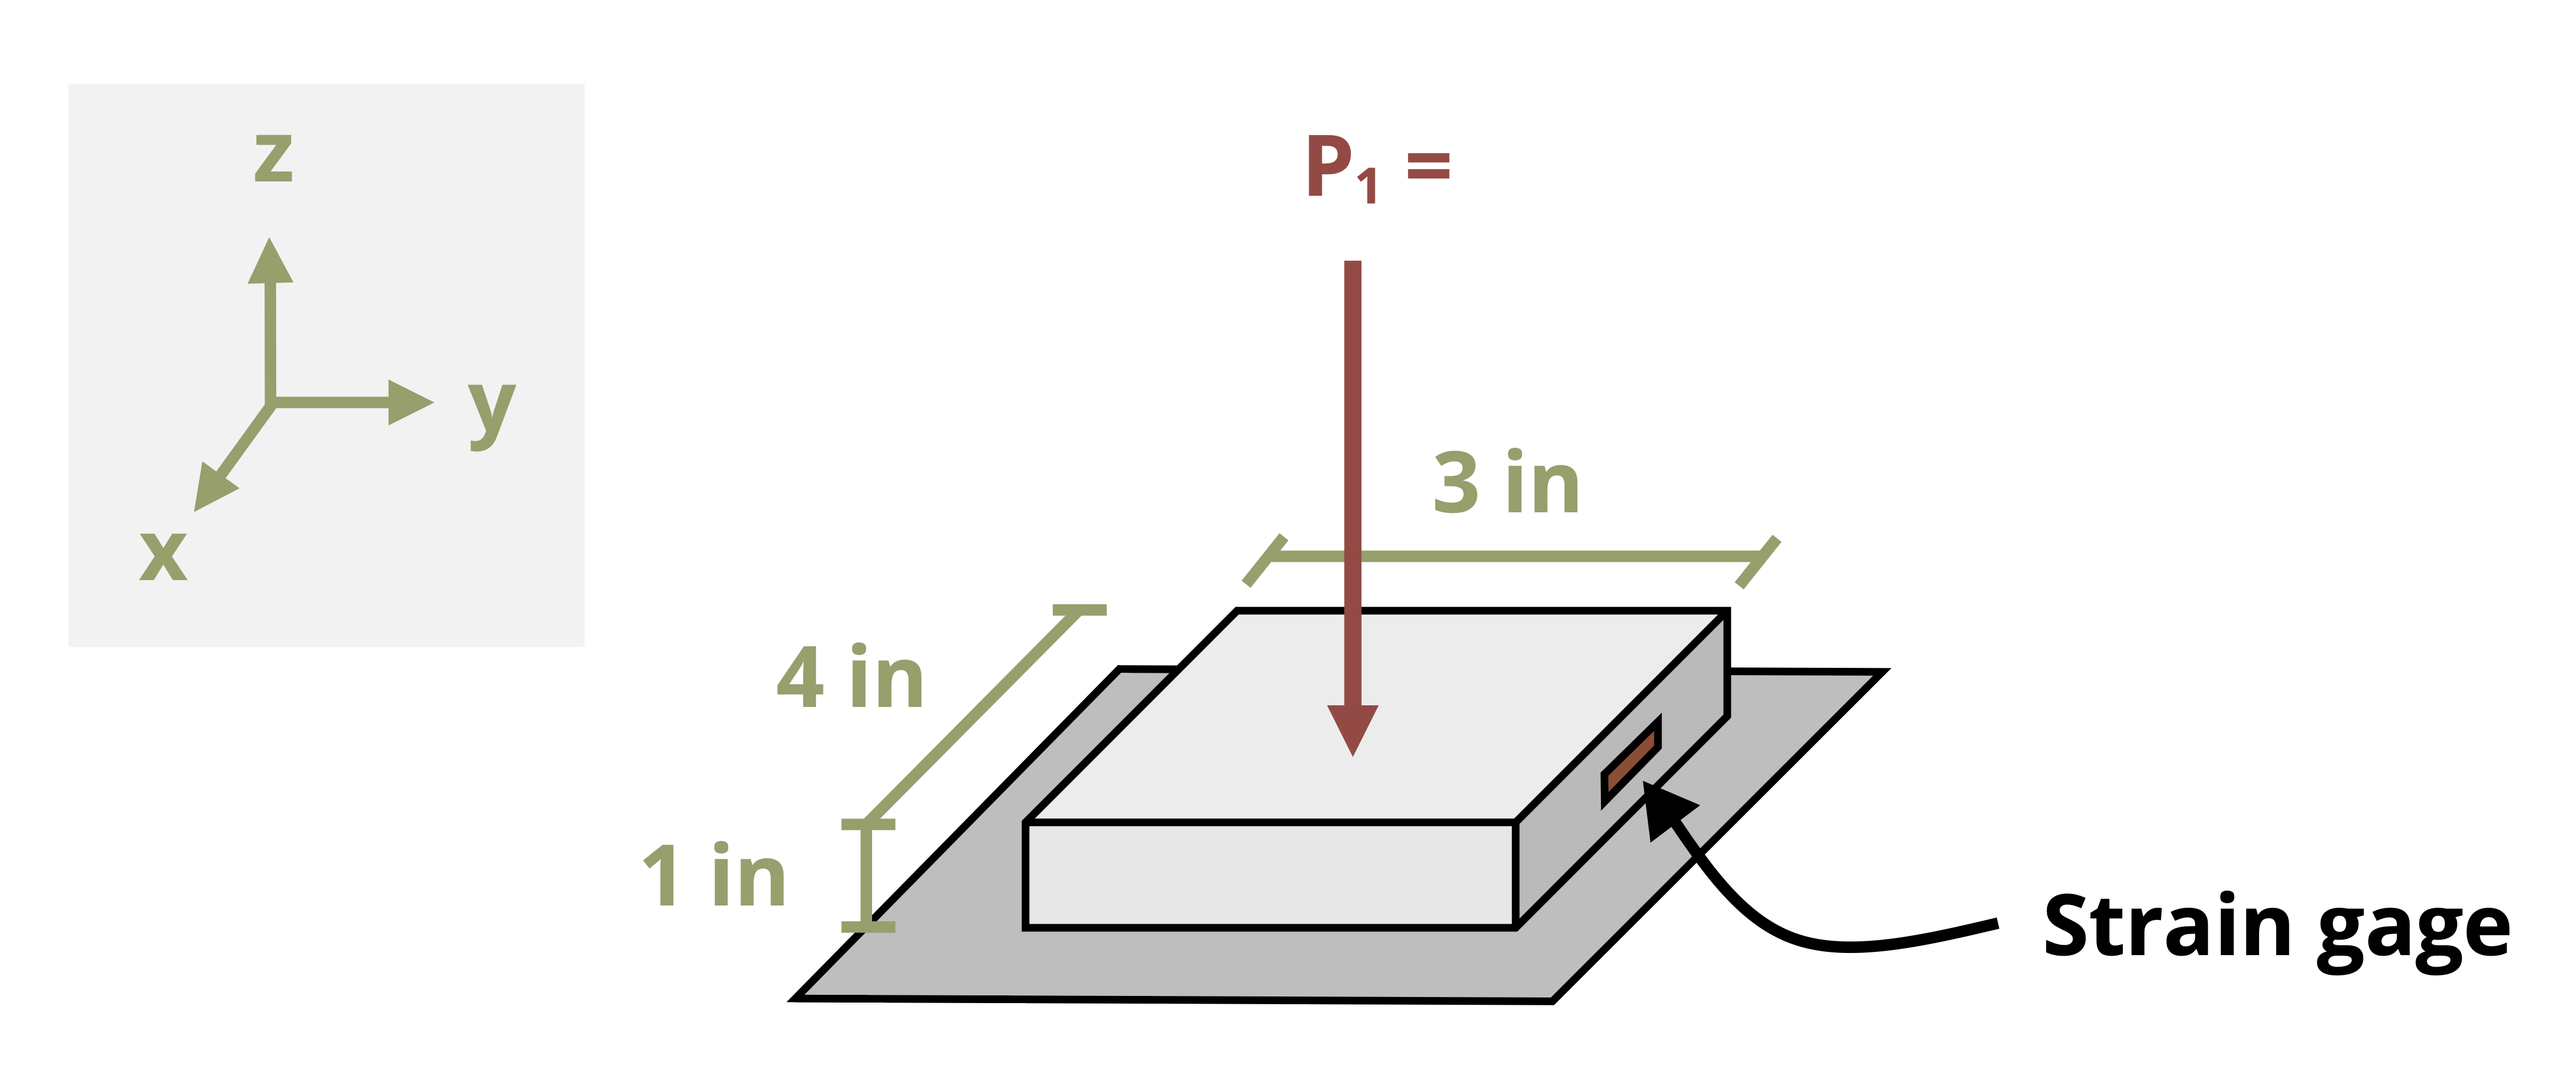
\includegraphics{images/205.png}

}

\caption{Figure 1: A strain gauge is placed on a test sample and a
vertical load is applied to the test sample.}

\end{figure}%

\begin{Shaded}
\begin{Highlighting}[]
\NormalTok{\#| standalone: true}
\NormalTok{\#| viewerHeight: 600}
\NormalTok{\#| components: [viewer]}

\NormalTok{from shiny import App, render, ui, reactive}
\NormalTok{import random}
\NormalTok{import asyncio}
\NormalTok{import io}
\NormalTok{import math}
\NormalTok{import string}
\NormalTok{from datetime import datetime}
\NormalTok{from pathlib import Path}

\NormalTok{def generate\_random\_letters(length):}
\NormalTok{    \# Generate a random string of letters of specified length}
\NormalTok{    return \textquotesingle{}\textquotesingle{}.join(random.choice(string.ascii\_lowercase) for \_ in range(length)) }

\NormalTok{problem\_ID="205"}
\NormalTok{P1=reactive.Value("\_\_")}
\NormalTok{E=reactive.Value("\_\_")}
\NormalTok{v=reactive.Value("\_\_")}
\NormalTok{SG=reactive.Value("\_\_")}

\NormalTok{attempts=["Timestamp,Attempt,Answer,Feedback\textbackslash{}n"]}

\NormalTok{app\_ui = ui.page\_fluid(}
\NormalTok{    ui.markdown("**Please enter your ID number from your instructor and click to generate your problem**"),}
\NormalTok{    ui.input\_text("ID","", placeholder="Enter ID Number Here"),}
\NormalTok{    ui.input\_action\_button("generate\_problem", "Generate Problem", class\_="btn{-}primary"),}
\NormalTok{    ui.markdown("**Problem Statement**"),}
\NormalTok{    ui.output\_ui("ui\_problem\_statement"),}
\NormalTok{    ui.input\_text("answer","Your Answer in percent", placeholder="Please enter your answer"),}
\NormalTok{    ui.input\_action\_button("submit", "Submit Answer", class\_="btn{-}primary"),}
\NormalTok{    ui.download\_button("download", "Download File to Submit", class\_="btn{-}success"),}
\NormalTok{)}

\NormalTok{def server(input, output, session):}
\NormalTok{    \# Initialize a counter for attempts}
\NormalTok{    attempt\_counter = reactive.Value(0)}

\NormalTok{    @output}
\NormalTok{    @render.ui}
\NormalTok{    def ui\_problem\_statement():}
\NormalTok{        return[ui.markdown(f"A strain gauge is placed on a polymer test sample with an elastic modulus E =  \{E()\} x 10\textless{}sup\textgreater{}6\textless{}/sup\textgreater{} psi and a Poisson\textquotesingle{}s ratio of v = \{v()\}. When a P\textless{}sub\textgreater{}1\textless{}/sub\textgreater{} = \{P1()\} kip vertical load is applied to the test sample, the strain gauge reads a strain of SG = \{SG()\} x 10\textless{}sup\textgreater{}{-}6\textless{}/sup\textgreater{} in the x{-}direction. What is the relative error of the strain gauge compared to the theoretical strain of the test sample? Note: relative error is defined to be the difference between the measured value and the theoretical value divided by the theoretical value ")]}
    
\NormalTok{    @reactive.Effect}
\NormalTok{    @reactive.event(input.generate\_problem)}
\NormalTok{    def randomize\_vars():}
\NormalTok{        random.seed(input.ID())}
\NormalTok{        P1.set(random.randrange(20, 200, 1)/10)}
\NormalTok{        E.set(random.randrange(5, 20, 1))}
\NormalTok{        v.set(random.randrange(20, 40, 1)/100)}
\NormalTok{        SG.set(round((v()*P1()*1000)/(12*E()),1){-}(random.randrange(3, 20, 1)/10))}
        
\NormalTok{    @reactive.Effect}
\NormalTok{    @reactive.event(input.submit)}
\NormalTok{    def \_():}
\NormalTok{        attempt\_counter.set(attempt\_counter() + 1)  \# Increment the attempt counter on each submission.}
\NormalTok{        sigmaz = ({-}P1()*1000)/(4*3)}
\NormalTok{        Ex = (({-}v()*(sigmaz))/(E()*10**6))}
\NormalTok{        instr=  ((Ex {-} SG()*10**{-}6)/Ex)*100}
\NormalTok{        if math.isclose(float(input.answer()), instr, rel\_tol=0.01):}
\NormalTok{            check = "*Correct*"}
\NormalTok{            correct\_indicator = "JL"}
\NormalTok{        else:}
\NormalTok{            check = "*Not Correct.*"}
\NormalTok{            correct\_indicator = "JG"}

\NormalTok{        \# Generate random parts for the encoded attempt.}
\NormalTok{        random\_start = generate\_random\_letters(4)}
\NormalTok{        random\_middle = generate\_random\_letters(4)}
\NormalTok{        random\_end = generate\_random\_letters(4)}
\NormalTok{        encoded\_attempt = f"\{random\_start\}\{problem\_ID\}{-}\{random\_middle\}\{attempt\_counter()\}\{correct\_indicator\}{-}\{random\_end\}\{input.ID()\}"}

\NormalTok{        \# Store the most recent encoded attempt in a reactive value so it persists across submissions}
\NormalTok{        session.encoded\_attempt = reactive.Value(encoded\_attempt)}

\NormalTok{        \# Append the attempt data to the attempts list without the encoded attempt}
\NormalTok{        attempts.append(f"\{datetime.now()\}, \{attempt\_counter()\}, \{input.answer()\}, \{check\}\textbackslash{}n")}

\NormalTok{        \# Show feedback to the user.}
\NormalTok{        feedback = ui.markdown(f"Your answer of \{input.answer()\} is \{check\}.")}
\NormalTok{        m = ui.modal(}
\NormalTok{            feedback,}
\NormalTok{            title="Feedback",}
\NormalTok{            easy\_close=True}
\NormalTok{        )}
\NormalTok{        ui.modal\_show(m)}

\NormalTok{    @session.download(filename=lambda: f"Problem\_Log{-}\{problem\_ID\}{-}\{input.ID()\}.csv")}
\NormalTok{    async def download():}
\NormalTok{        \# Start the CSV with the encoded attempt (without label)}
\NormalTok{        final\_encoded = session.encoded\_attempt() if session.encoded\_attempt is not None else "No attempts"}
\NormalTok{        yield f"\{final\_encoded\}\textbackslash{}n\textbackslash{}n"}
        
\NormalTok{        \# Write the header for the remaining CSV data once}
\NormalTok{        yield "Timestamp,Attempt,Answer,Feedback\textbackslash{}n"}
        
\NormalTok{        \# Write the attempts data, ensure that the header from the attempts list is not written again}
\NormalTok{        for attempt in attempts[1:]:  \# Skip the first element which is the header}
\NormalTok{            await asyncio.sleep(0.25)  \# This delay may not be necessary; adjust as needed}
\NormalTok{            yield attempt}

\NormalTok{\# App installation}
\NormalTok{app = App(app\_ui, server)}
\end{Highlighting}
\end{Shaded}

\chapter*{Problem 4.25}\label{problem-4.25}
\addcontentsline{toc}{chapter}{Problem 4.25}

\markboth{Problem 4.25}{Problem 4.25}

This is a dynamic rendering of the problem with dynamic variables based
on the username entered.

\section*{Problem Image}\label{problem-image-39}
\addcontentsline{toc}{section}{Problem Image}

\markright{Problem Image}

\begin{figure}[H]

{\centering 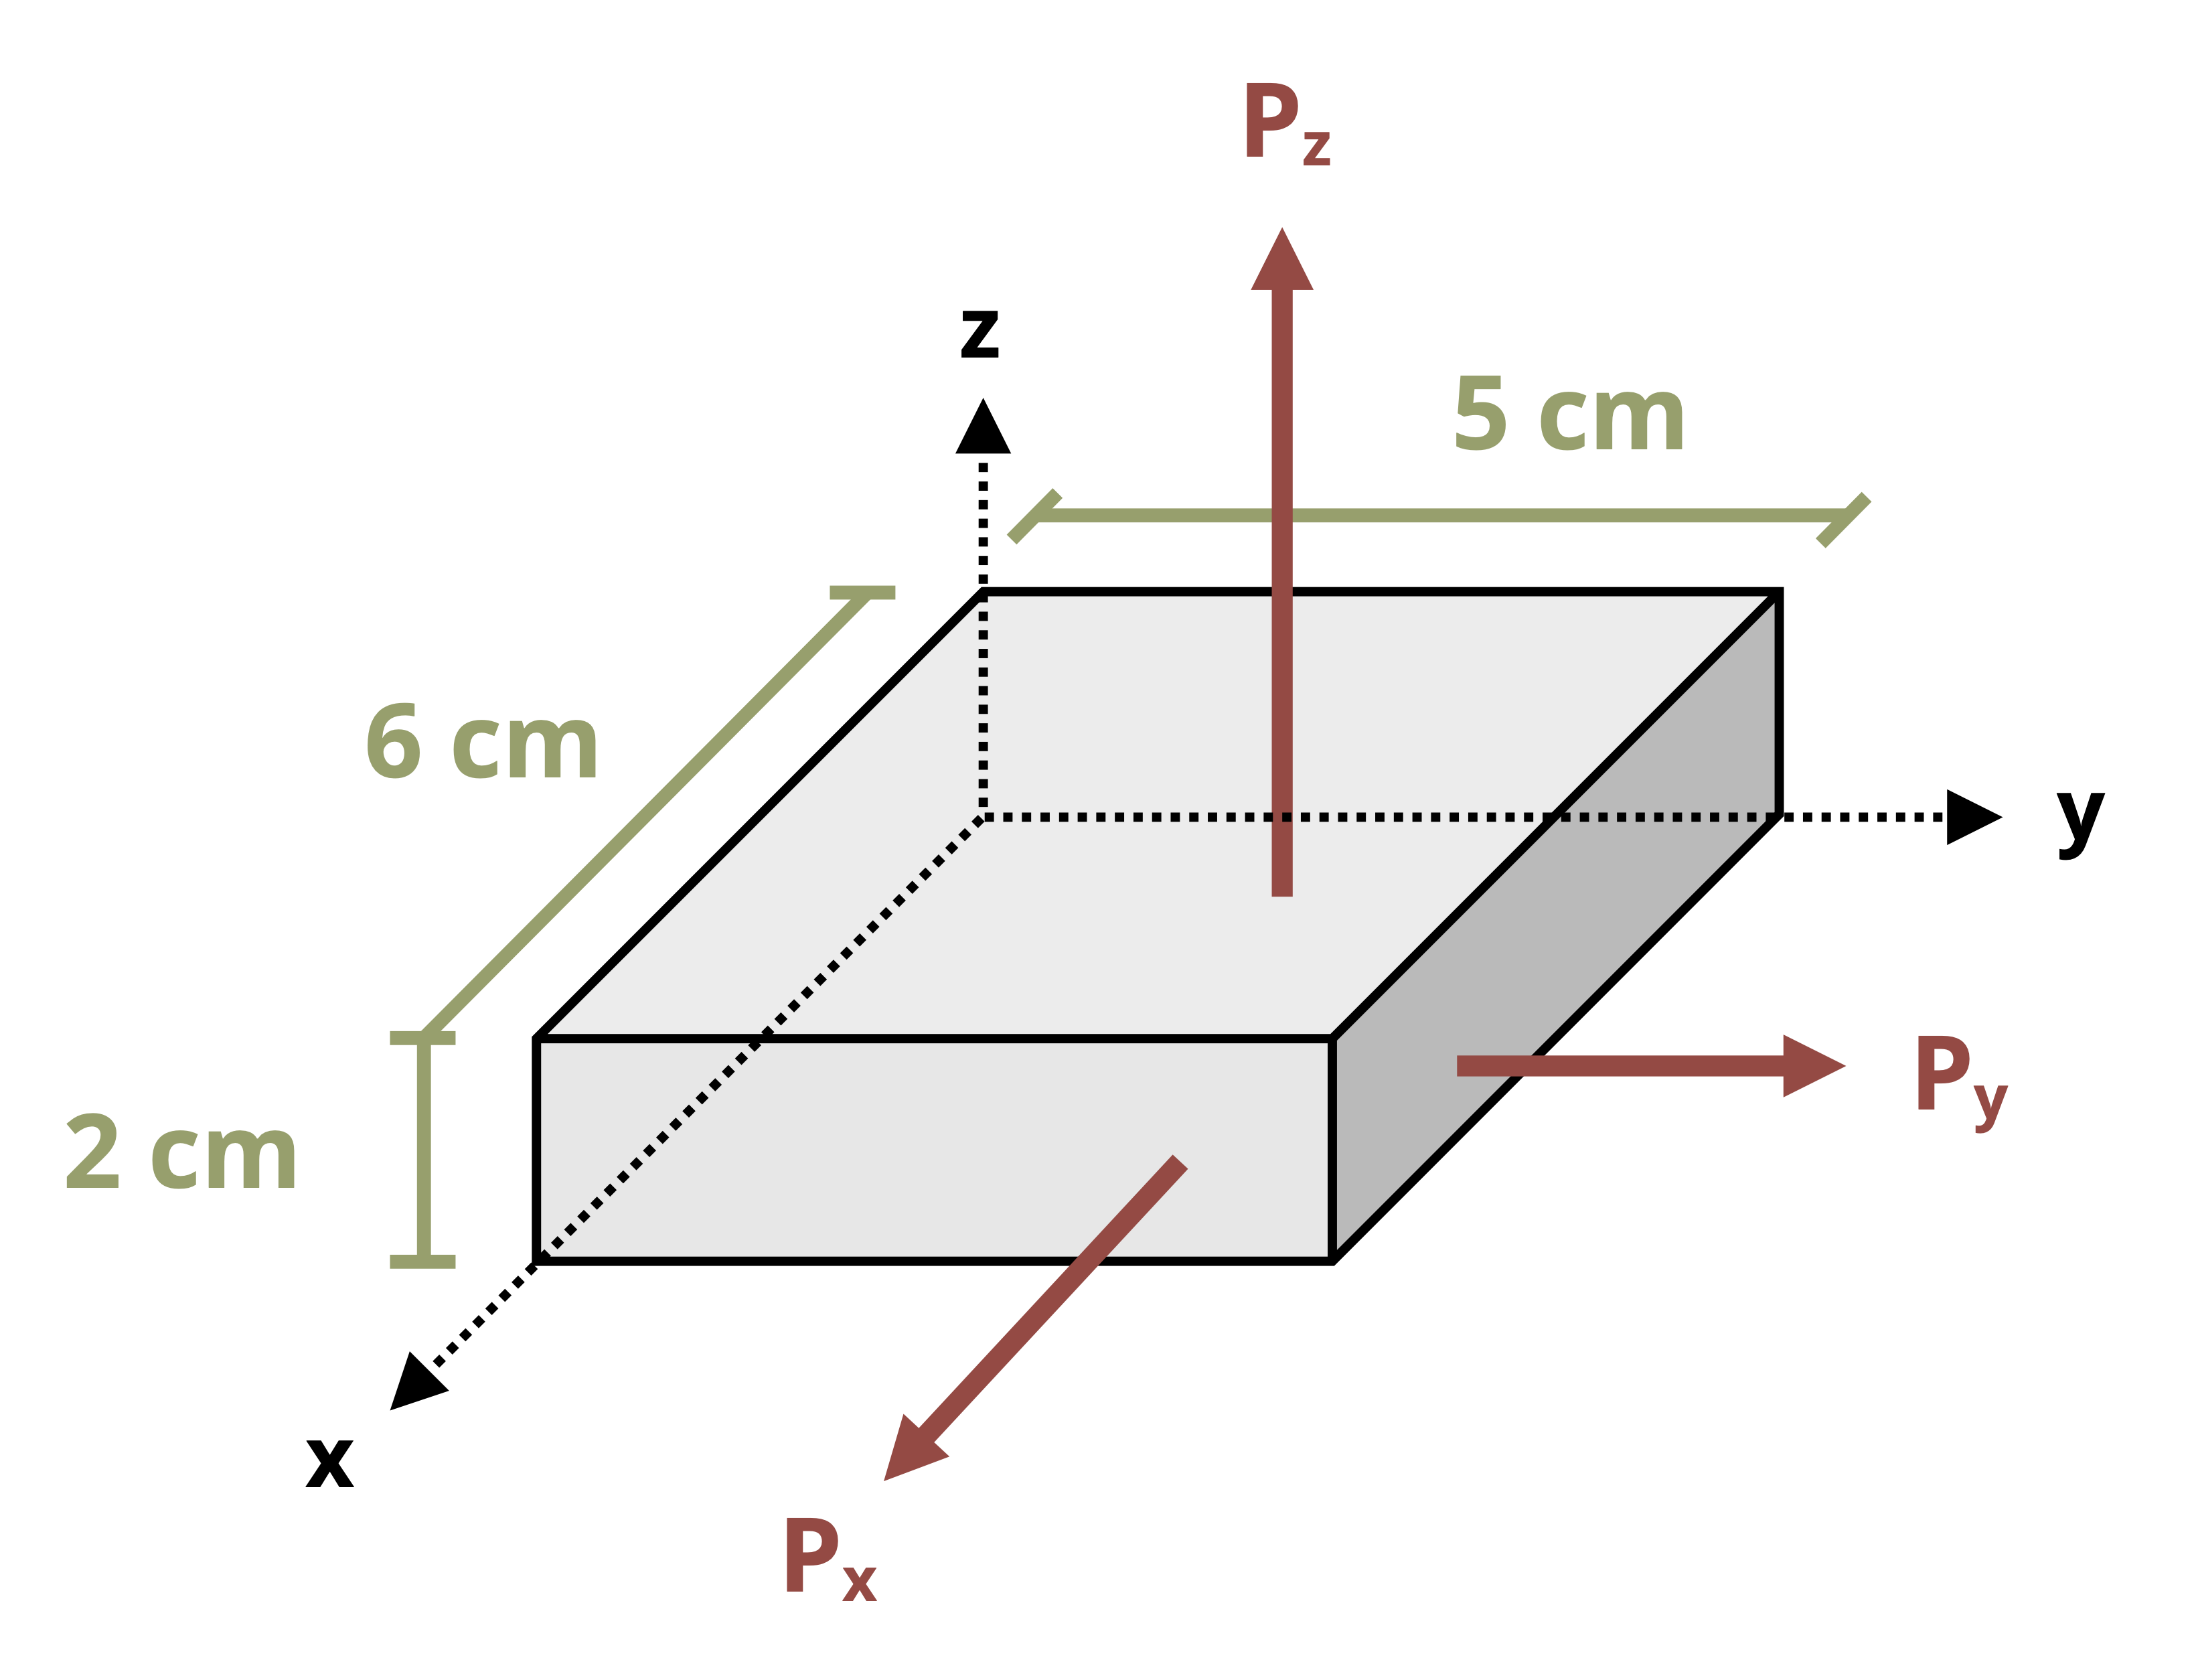
\includegraphics{images/208.png}

}

\caption{Figure 1: A block is pulled in all three directions.}

\end{figure}%

\begin{Shaded}
\begin{Highlighting}[]
\NormalTok{\#| standalone: true}
\NormalTok{\#| viewerHeight: 600}
\NormalTok{\#| components: [viewer]}

\NormalTok{from shiny import App, render, ui, reactive}
\NormalTok{import random}
\NormalTok{import asyncio}
\NormalTok{import io}
\NormalTok{import math}
\NormalTok{import string}
\NormalTok{from datetime import datetime}
\NormalTok{from pathlib import Path}

\NormalTok{def generate\_random\_letters(length):}
\NormalTok{    \# Generate a random string of letters of specified length}
\NormalTok{    return \textquotesingle{}\textquotesingle{}.join(random.choice(string.ascii\_lowercase) for \_ in range(length)) }

\NormalTok{problem\_ID="208"}
\NormalTok{Px=reactive.Value("\_\_")}
\NormalTok{Py=reactive.Value("\_\_")}
\NormalTok{Pz=reactive.Value("\_\_")}
\NormalTok{L=reactive.Value("\_\_")}
\NormalTok{E=reactive.Value("\_\_")}
\NormalTok{v=reactive.Value("\_\_")}


\NormalTok{attempts=["Timestamp,Attempt,Answer,Feedback\textbackslash{}n"]}

\NormalTok{app\_ui = ui.page\_fluid(}
\NormalTok{    ui.markdown("**Please enter your ID number from your instructor and click to generate your problem**"),}
\NormalTok{    ui.input\_text("ID","", placeholder="Enter ID Number Here"),}
\NormalTok{    ui.input\_action\_button("generate\_problem", "Generate Problem", class\_="btn{-}primary"),}
\NormalTok{    ui.markdown("**Problem Statement**"),}
\NormalTok{    ui.output\_ui("ui\_problem\_statement"),}
\NormalTok{    ui.input\_text("answer","Your Answer in percent", placeholder="Please enter your answer"),}
\NormalTok{    ui.input\_action\_button("submit", "Submit Answer", class\_="btn{-}primary"),}
\NormalTok{    ui.download\_button("download", "Download File to Submit", class\_="btn{-}success"),}
\NormalTok{)}


\NormalTok{def server(input, output, session):}
\NormalTok{    \# Initialize a counter for attempts}
\NormalTok{    attempt\_counter = reactive.Value(0)}

\NormalTok{    @output}
\NormalTok{    @render.ui}
\NormalTok{    def ui\_problem\_statement():}
\NormalTok{        return[ui.markdown(f"A block is pulled in all three directions (P\textless{}sub\textgreater{}x\textless{}/sub\textgreater{} = \{Px()\} kN, P\textless{}sub\textgreater{}y\textless{}/sub\textgreater{} = \{Py()\} kN, P\textless{}sub\textgreater{}z\textless{}/sub\textgreater{} = \{Pz()\} kN). What is the percent change in volume after all three loads are applied? Assume E = \{E()\} MPa and v = \{v()\}. ")]}
    
\NormalTok{    @reactive.Effect}
\NormalTok{    @reactive.event(input.generate\_problem)}
\NormalTok{    def randomize\_vars():}
\NormalTok{        random.seed(input.ID())}
\NormalTok{        Px.set(random.randrange(1, 20, 1))}
\NormalTok{        Py.set(random.randrange(1, 20, 1))}
\NormalTok{        Pz.set(random.randrange(1, 20, 1))}
\NormalTok{        E.set(random.randrange(1000, 2000, 100))}
\NormalTok{        v.set(random.randrange(20, 40, 1)/100)}
        
\NormalTok{    @reactive.Effect}
\NormalTok{    @reactive.event(input.submit)}
\NormalTok{    def \_():}
\NormalTok{        attempt\_counter.set(attempt\_counter() + 1)  \# Increment the attempt counter on each submission.}
\NormalTok{        sigmax = (Px()/(5*2))*10}
\NormalTok{        sigmay = (Py()/(6*2))*10}
\NormalTok{        sigmaz = (Pz()/(5*6))*10}
\NormalTok{        Ex = (sigmax {-} v()*(sigmay+sigmaz))/(E())}
\NormalTok{        Ey = (sigmay {-} v()*(sigmaz+sigmax))/(E())}
\NormalTok{        Ez = (sigmaz {-} v()*(sigmax+sigmay))/(E())}
\NormalTok{        Lx = 6 + 6*Ex}
\NormalTok{        Ly = 5 + 5*Ey}
\NormalTok{        Lz = 2 + 2*Ez}
\NormalTok{        instr= (((Lx*Ly*Lz){-}60)/60)*100}
\NormalTok{        if math.isclose(float(input.answer()), instr, rel\_tol=0.01):}
\NormalTok{            check = "*Correct*"}
\NormalTok{            correct\_indicator = "JL"}
\NormalTok{        else:}
\NormalTok{            check = "*Not Correct.*"}
\NormalTok{            correct\_indicator = "JG"}

\NormalTok{        \# Generate random parts for the encoded attempt.}
\NormalTok{        random\_start = generate\_random\_letters(4)}
\NormalTok{        random\_middle = generate\_random\_letters(4)}
\NormalTok{        random\_end = generate\_random\_letters(4)}
\NormalTok{        encoded\_attempt = f"\{random\_start\}\{problem\_ID\}{-}\{random\_middle\}\{attempt\_counter()\}\{correct\_indicator\}{-}\{random\_end\}\{input.ID()\}"}

\NormalTok{        \# Store the most recent encoded attempt in a reactive value so it persists across submissions}
\NormalTok{        session.encoded\_attempt = reactive.Value(encoded\_attempt)}

\NormalTok{        \# Append the attempt data to the attempts list without the encoded attempt}
\NormalTok{        attempts.append(f"\{datetime.now()\}, \{attempt\_counter()\}, \{input.answer()\}, \{check\}\textbackslash{}n")}

\NormalTok{        \# Show feedback to the user.}
\NormalTok{        feedback = ui.markdown(f"Your answer of \{input.answer()\} is \{check\}.")}
\NormalTok{        m = ui.modal(}
\NormalTok{            feedback,}
\NormalTok{            title="Feedback",}
\NormalTok{            easy\_close=True}
\NormalTok{        )}
\NormalTok{        ui.modal\_show(m)}

\NormalTok{    @session.download(filename=lambda: f"Problem\_Log{-}\{problem\_ID\}{-}\{input.ID()\}.csv")}
\NormalTok{    async def download():}
\NormalTok{        \# Start the CSV with the encoded attempt (without label)}
\NormalTok{        final\_encoded = session.encoded\_attempt() if session.encoded\_attempt is not None else "No attempts"}
\NormalTok{        yield f"\{final\_encoded\}\textbackslash{}n\textbackslash{}n"}
        
\NormalTok{        \# Write the header for the remaining CSV data once}
\NormalTok{        yield "Timestamp,Attempt,Answer,Feedback\textbackslash{}n"}
        
\NormalTok{        \# Write the attempts data, ensure that the header from the attempts list is not written again}
\NormalTok{        for attempt in attempts[1:]:  \# Skip the first element which is the header}
\NormalTok{            await asyncio.sleep(0.25)  \# This delay may not be necessary; adjust as needed}
\NormalTok{            yield attempt}


\NormalTok{\# App installation}
\NormalTok{app = App(app\_ui, server)}
\end{Highlighting}
\end{Shaded}

\chapter*{Problem 4.35}\label{problem-4.35-1}
\addcontentsline{toc}{chapter}{Problem 4.35}

\markboth{Problem 4.35}{Problem 4.35}

This is a dynamic rendering of the problem with dynamic variables based
on the username entered.

\section*{Problem Image}\label{problem-image-40}
\addcontentsline{toc}{section}{Problem Image}

\markright{Problem Image}

\begin{figure}[H]

{\centering 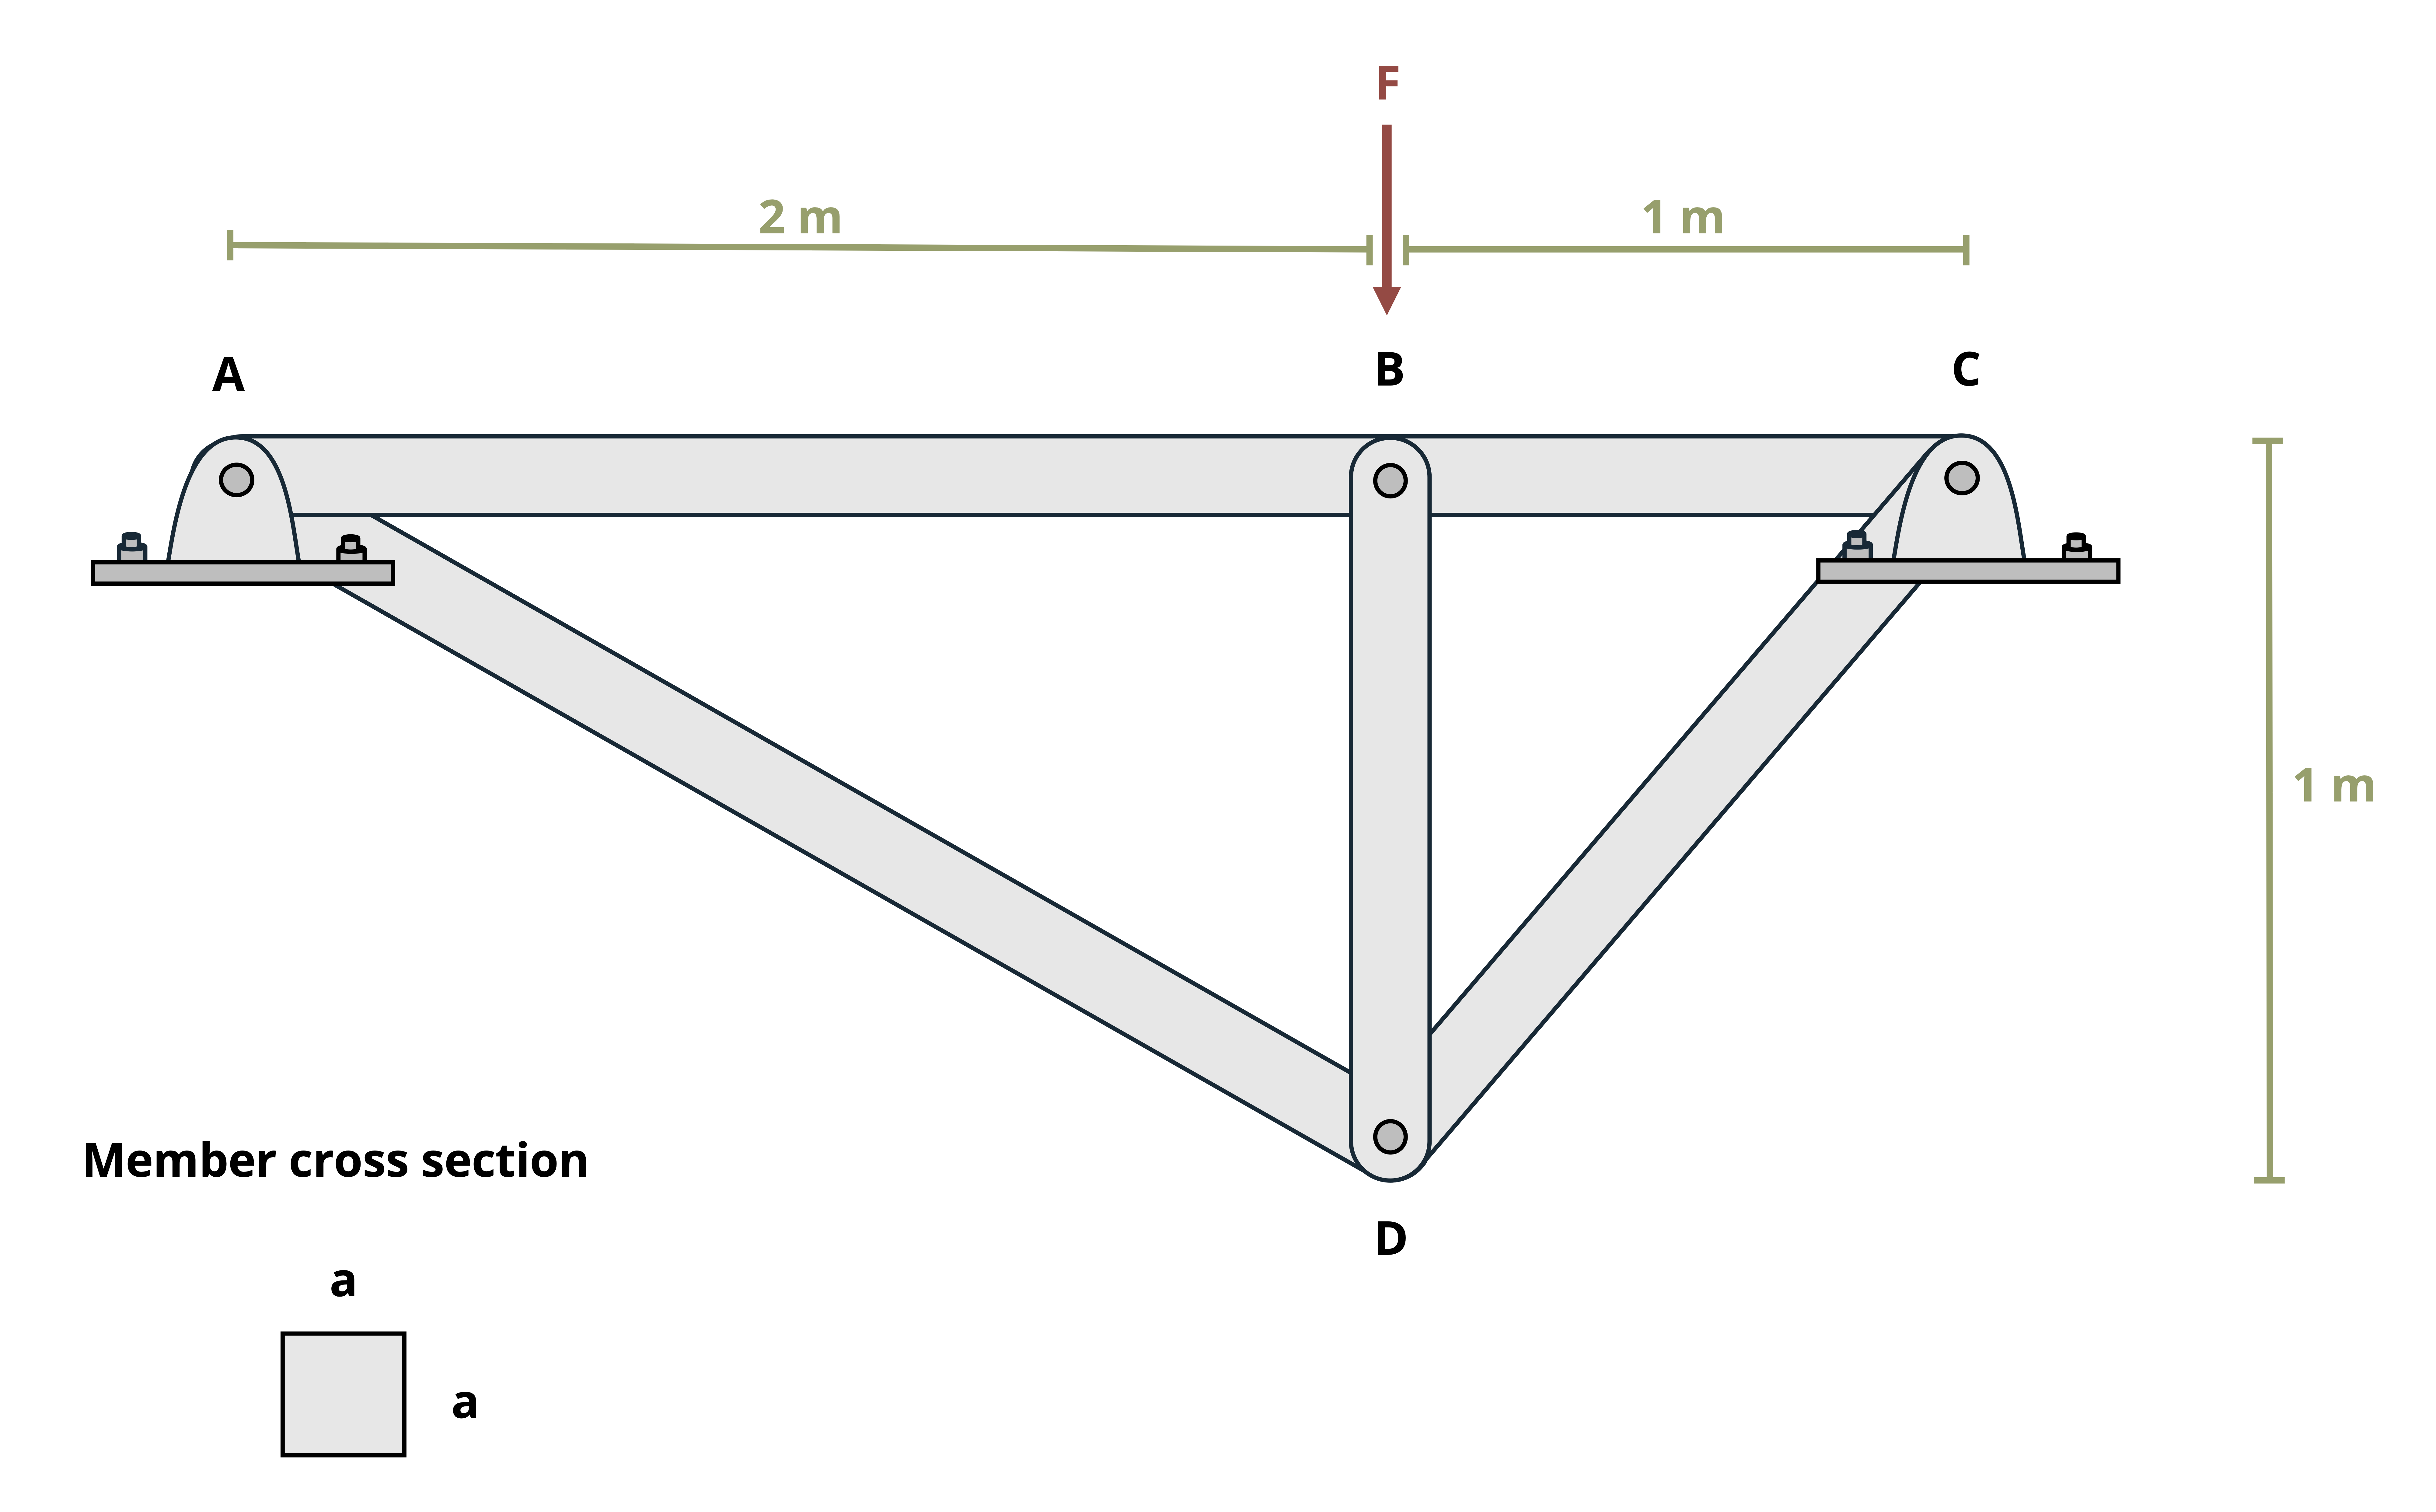
\includegraphics{images/157.png}

}

\caption{Figure 1: A small truss is constructed with solid square wood
members.}

\end{figure}%

\begin{Shaded}
\begin{Highlighting}[]
\NormalTok{\#| standalone: true}
\NormalTok{\#| viewerHeight: 600}
\NormalTok{\#| components: [viewer]}

\NormalTok{from shiny import App, render, ui, reactive}
\NormalTok{import random}
\NormalTok{import asyncio}
\NormalTok{import io}
\NormalTok{import math}
\NormalTok{import string}
\NormalTok{from datetime import datetime}
\NormalTok{from pathlib import Path}

\NormalTok{def generate\_random\_letters(length):}
\NormalTok{    \# Generate a random string of letters of specified length}
\NormalTok{    return \textquotesingle{}\textquotesingle{}.join(random.choice(string.ascii\_lowercase) for \_ in range(length))  }

\NormalTok{problem\_ID="157"}
\NormalTok{F=reactive.Value("\_\_")}
\NormalTok{FS=reactive.Value("\_\_")}
\NormalTok{σfail=reactive.Value("\_\_")}

\NormalTok{attempts=["Timestamp,Attempt,Answer,Feedback\textbackslash{}n"]}

\NormalTok{app\_ui = ui.page\_fluid(}
\NormalTok{    ui.markdown("**Please enter your ID number from your instructor and click to generate your problem**"),}
\NormalTok{    ui.input\_text("ID","", placeholder="Enter ID Number Here"),}
\NormalTok{    ui.input\_action\_button("generate\_problem", "Generate Problem", class\_="btn{-}primary"),}
\NormalTok{    ui.markdown("**Problem Statement**"),}
\NormalTok{    ui.output\_ui("ui\_problem\_statement"),}
\NormalTok{    ui.input\_text("answer","Your Answer in units of centimeters", placeholder="Please enter your answer"),}
\NormalTok{    ui.input\_action\_button("submit", "Submit Answer", class\_="btn{-}primary"),}
\NormalTok{    ui.download\_button("download", "Download File to Submit", class\_="btn{-}success"),}
\NormalTok{)}


\NormalTok{def server(input, output, session):}
\NormalTok{    \# Initialize a counter for attempts}
\NormalTok{    attempt\_counter = reactive.Value(0)}

\NormalTok{    @output}
\NormalTok{    @render.ui}
\NormalTok{    def ui\_problem\_statement():}
\NormalTok{        return[ui.markdown(f"A small truss is constructed with solid square wood members and subjected to a load of F = \{F()\} kN. Determine the minimum dimension, a, of the member so that the truss will have a factor of safety of \{FS()\}. All members have the same cross{-}section. The wood has a failure stress of σ\textless{}sub\textgreater{}fail\textless{}/sub\textgreater{} = \{σfail()\} MPa.")]}
    
\NormalTok{    @reactive.Effect}
\NormalTok{    @reactive.event(input.generate\_problem)}
\NormalTok{    def randomize\_vars():}
\NormalTok{        random.seed(input.ID())}
\NormalTok{        F.set(random.randrange(15, 50, 1))}
\NormalTok{        FS.set(random.randrange(15, 40, 1)/10)}
\NormalTok{        σfail.set(random.randrange(40, 60, 1))}
        

\NormalTok{    @reactive.Effect}
\NormalTok{    @reactive.event(input.submit)}
\NormalTok{    def \_():}
\NormalTok{        attempt\_counter.set(attempt\_counter() + 1)  \# Increment the attempt counter on each submission.}
    
\NormalTok{        dl = FS()*F()}
\NormalTok{        A = (dl/(σfail()*10**3))*100*100}
\NormalTok{        instr= math.sqrt(A)}
\NormalTok{        if math.isclose(float(input.answer()), instr, rel\_tol=0.01):}
\NormalTok{            check = "*Correct*"}
\NormalTok{            correct\_indicator = "JL"}
\NormalTok{        else:}
\NormalTok{            check = "*Not Correct.*"}
\NormalTok{            correct\_indicator = "JG"}

\NormalTok{        \# Generate random parts for the encoded attempt.}
\NormalTok{        random\_start = generate\_random\_letters(4)}
\NormalTok{        random\_middle = generate\_random\_letters(4)}
\NormalTok{        random\_end = generate\_random\_letters(4)}
\NormalTok{        encoded\_attempt = f"\{random\_start\}\{problem\_ID\}{-}\{random\_middle\}\{attempt\_counter()\}\{correct\_indicator\}{-}\{random\_end\}\{input.ID()\}"}

\NormalTok{        \# Store the most recent encoded attempt in a reactive value so it persists across submissions}
\NormalTok{        session.encoded\_attempt = reactive.Value(encoded\_attempt)}

\NormalTok{        \# Append the attempt data to the attempts list without the encoded attempt}
\NormalTok{        attempts.append(f"\{datetime.now()\}, \{attempt\_counter()\}, \{input.answer()\}, \{check\}\textbackslash{}n")}

\NormalTok{        \# Show feedback to the user.}
\NormalTok{        feedback = ui.markdown(f"Your answer of \{input.answer()\} is \{check\}.")}
\NormalTok{        m = ui.modal(}
\NormalTok{            feedback,}
\NormalTok{            title="Feedback",}
\NormalTok{            easy\_close=True}
\NormalTok{        )}
\NormalTok{        ui.modal\_show(m)}

\NormalTok{    @session.download(filename=lambda: f"Problem\_Log{-}\{problem\_ID\}{-}\{input.ID()\}.csv")}
\NormalTok{    async def download():}
\NormalTok{        \# Start the CSV with the encoded attempt (without label)}
\NormalTok{        final\_encoded = session.encoded\_attempt() if session.encoded\_attempt is not None else "No attempts"}
\NormalTok{        yield f"\{final\_encoded\}\textbackslash{}n\textbackslash{}n"}
        
\NormalTok{        \# Write the header for the remaining CSV data once}
\NormalTok{        yield "Timestamp,Attempt,Answer,Feedback\textbackslash{}n"}
        
\NormalTok{        \# Write the attempts data, ensure that the header from the attempts list is not written again}
\NormalTok{        for attempt in attempts[1:]:  \# Skip the first element which is the header}
\NormalTok{            await asyncio.sleep(0.25)  \# This delay may not be necessary; adjust as needed}
\NormalTok{            yield attempt}


\NormalTok{\# App installation}
\NormalTok{app = App(app\_ui, server)}
\end{Highlighting}
\end{Shaded}

\chapter*{Problem 5.11}\label{problem-5.11}
\addcontentsline{toc}{chapter}{Problem 5.11}

\markboth{Problem 5.11}{Problem 5.11}

This is a dynamic rendering of the problem with dynamic variables based
on the username entered.

\section*{Problem Image}\label{problem-image-41}
\addcontentsline{toc}{section}{Problem Image}

\markright{Problem Image}

\begin{figure}[H]

{\centering 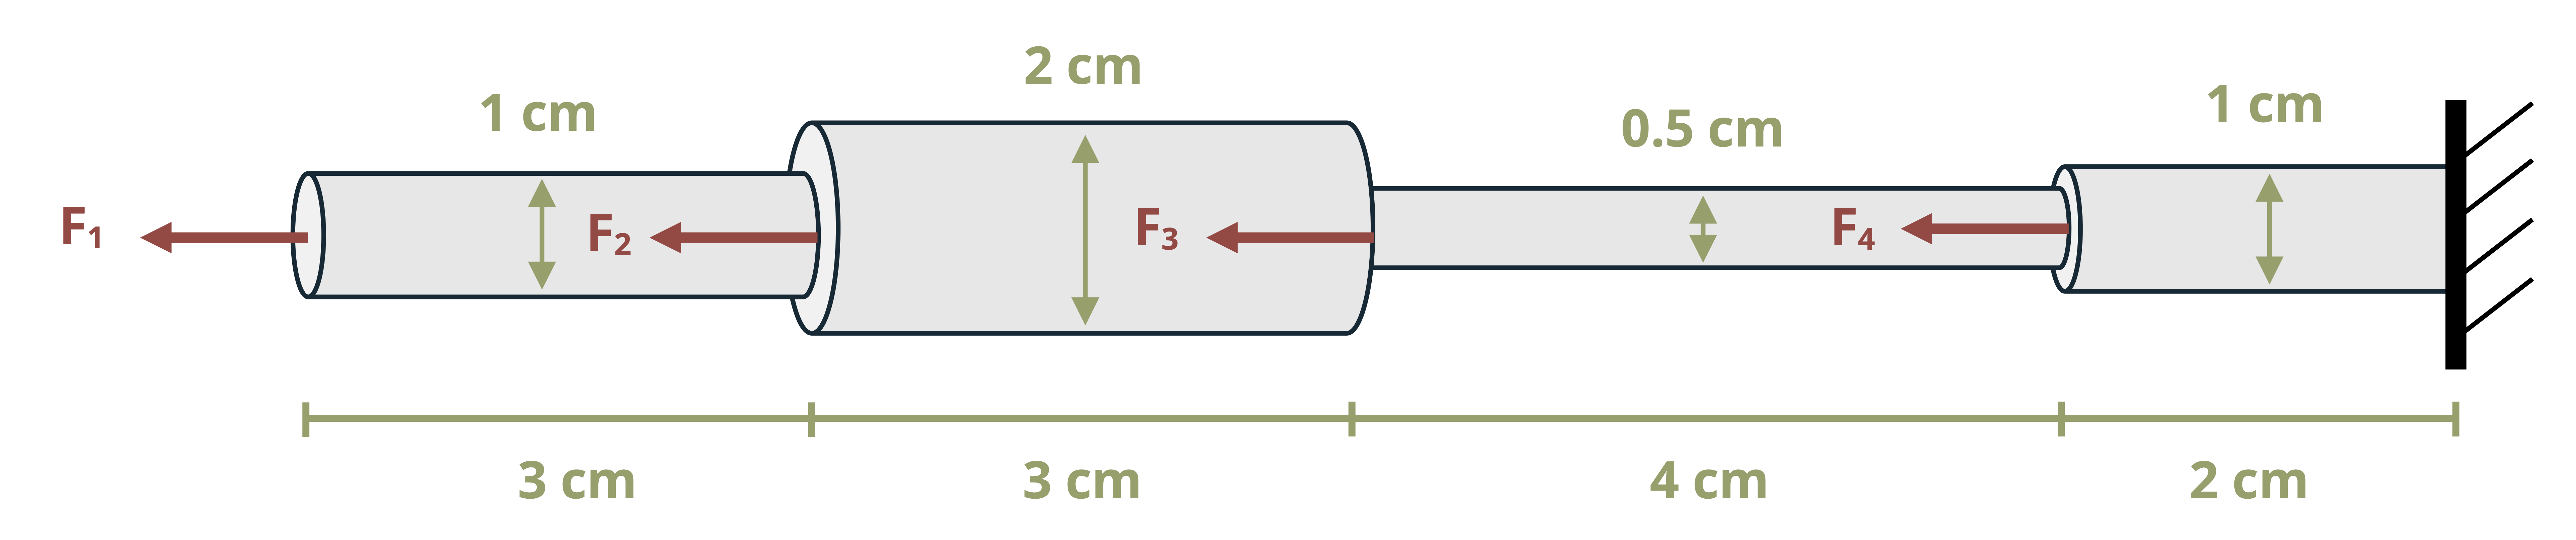
\includegraphics{images/183.png}

}

\caption{Figure 1: A series of solid, steel, circular bars are loaded
with forces.}

\end{figure}%

\begin{Shaded}
\begin{Highlighting}[]
\NormalTok{\#| standalone: true}
\NormalTok{\#| viewerHeight: 600}
\NormalTok{\#| components: [viewer]}

\NormalTok{from shiny import App, render, ui, reactive}
\NormalTok{import random}
\NormalTok{import asyncio}
\NormalTok{import io}
\NormalTok{import math}
\NormalTok{import string}
\NormalTok{from datetime import datetime}
\NormalTok{from pathlib import Path}

\NormalTok{problem\_ID="183"}
\NormalTok{F1=reactive.Value("\_\_")}
\NormalTok{F2=reactive.Value("\_\_")}
\NormalTok{F3=reactive.Value("\_\_")}
\NormalTok{F4=reactive.Value("\_\_")}
\NormalTok{E=210}

\NormalTok{def generate\_random\_letters(length):}
\NormalTok{    \# Generate a random string of letters of specified length}
\NormalTok{    return \textquotesingle{}\textquotesingle{}.join(random.choice(string.ascii\_lowercase) for \_ in range(length))  }

\NormalTok{attempts=["Timestamp,Attempt,Answer,Feedback\textbackslash{}n"]}

\NormalTok{app\_ui = ui.page\_fluid(}
\NormalTok{    ui.markdown("**Please enter your ID number from your instructor and click to generate your problem**"),}
\NormalTok{    ui.input\_text("ID","", placeholder="Enter ID Number Here"),}
\NormalTok{    ui.input\_action\_button("generate\_problem", "Generate Problem", class\_="btn{-}primary"),}
\NormalTok{    ui.markdown("**Problem Statement**"),}
\NormalTok{    ui.output\_ui("ui\_problem\_statement"),}
\NormalTok{    ui.input\_text("answer","Your Answer in units of mm", placeholder="Please enter your answer"),}
\NormalTok{    ui.input\_action\_button("submit", "Submit Answer", class\_="btn{-}primary"),}
\NormalTok{    ui.download\_button("download", "Download File to Submit", class\_="btn{-}success"),}
\NormalTok{)}

\NormalTok{def server(input, output, session):}
\NormalTok{    \# Initialize a counter for attempts}
\NormalTok{    attempt\_counter = reactive.Value(0)}

\NormalTok{    @output}
\NormalTok{    @render.ui}
\NormalTok{    def ui\_problem\_statement():}
\NormalTok{        return[ui.markdown(f"A series of solid, steel, circular bars are loaded with forces as shown, where F\textless{}sub\textgreater{}1\textless{}/sub\textgreater{} = \{F1()\} kN, F\textless{}sub\textgreater{}2\textless{}/sub\textgreater{} = \{F2()\} kN, F\textless{}sub\textgreater{}3\textless{}/sub\textgreater{} = \{F3()\} kN, and F\textless{}sub\textgreater{}4\textless{}/sub\textgreater{} = \{F4()\} kN. What is the total change in length of the system? Assume E = 210 GPa for steel.")]}
    
\NormalTok{    @reactive.Effect}
\NormalTok{    @reactive.event(input.generate\_problem)}
\NormalTok{    def randomize\_vars():}
\NormalTok{        random.seed(input.ID())}
\NormalTok{        F1.set(random.randrange(10, 100, 1)/10)}
\NormalTok{        F2.set(random.randrange(10, 100, 1)/10)}
\NormalTok{        F3.set(random.randrange(10, 100, 1)/10)}
\NormalTok{        F4.set(random.randrange(10, 100, 1)/10)}

\NormalTok{    @reactive.Effect}
\NormalTok{    @reactive.event(input.submit)}
\NormalTok{    def \_():}
\NormalTok{        attempt\_counter.set(attempt\_counter() + 1)  \# Increment the attempt counter on each submission.}
\NormalTok{        instr= ((F1()*3)/(E*math.pi*0.5**2)+((F1()+F2())*3)/(E*math.pi*1**2)+((F1()+F2()+F3())*4)/(E*math.pi*0.25**2)+((F1()+F2()+F3()+F4())*2)/(E*math.pi*0.5**2))/10}
\NormalTok{        if math.isclose(float(input.answer()), instr, rel\_tol=0.01):}
\NormalTok{            check = "*Correct*"}
\NormalTok{            correct\_indicator = "JL"}
\NormalTok{        else:}
\NormalTok{            check = "*Not Correct.*"}
\NormalTok{            correct\_indicator = "JG"}

\NormalTok{        \# Generate random parts for the encoded attempt.}
\NormalTok{        random\_start = generate\_random\_letters(4)}
\NormalTok{        random\_middle = generate\_random\_letters(4)}
\NormalTok{        random\_end = generate\_random\_letters(4)}
\NormalTok{        encoded\_attempt = f"\{random\_start\}\{problem\_ID\}{-}\{random\_middle\}\{attempt\_counter()\}\{correct\_indicator\}{-}\{random\_end\}\{input.ID()\}"}

\NormalTok{        \# Store the most recent encoded attempt in a reactive value so it persists across submissions}
\NormalTok{        session.encoded\_attempt = reactive.Value(encoded\_attempt)}

\NormalTok{        \# Append the attempt data to the attempts list without the encoded attempt}
\NormalTok{        attempts.append(f"\{datetime.now()\}, \{attempt\_counter()\}, \{input.answer()\}, \{check\}\textbackslash{}n")}

\NormalTok{        \# Show feedback to the user.}
\NormalTok{        feedback = ui.markdown(f"Your answer of \{input.answer()\} is \{check\}.")}
\NormalTok{        m = ui.modal(}
\NormalTok{            feedback,}
\NormalTok{            title="Feedback",}
\NormalTok{            easy\_close=True}
\NormalTok{        )}
\NormalTok{        ui.modal\_show(m)}

\NormalTok{    @session.download(filename=lambda: f"Problem\_Log{-}\{problem\_ID\}{-}\{input.ID()\}.csv")}
\NormalTok{    async def download():}
\NormalTok{        \# Start the CSV with the encoded attempt (without label)}
\NormalTok{        final\_encoded = session.encoded\_attempt() if session.encoded\_attempt is not None else "No attempts"}
\NormalTok{        yield f"\{final\_encoded\}\textbackslash{}n\textbackslash{}n"}
        
\NormalTok{        \# Write the header for the remaining CSV data once}
\NormalTok{        yield "Timestamp,Attempt,Answer,Feedback\textbackslash{}n"}
        
\NormalTok{        \# Write the attempts data, ensure that the header from the attempts list is not written again}
\NormalTok{        for attempt in attempts[1:]:  \# Skip the first element which is the header}
\NormalTok{            await asyncio.sleep(0.25)  \# This delay may not be necessary; adjust as needed}
\NormalTok{            yield attempt}

\NormalTok{\# App installation}
\NormalTok{app = App(app\_ui, server)}
\end{Highlighting}
\end{Shaded}

\chapter*{Problem 5.12}\label{problem-5.12}
\addcontentsline{toc}{chapter}{Problem 5.12}

\markboth{Problem 5.12}{Problem 5.12}

This is a dynamic rendering of the problem with dynamic variables based
on the username entered.

\section*{Problem Image}\label{problem-image-42}
\addcontentsline{toc}{section}{Problem Image}

\markright{Problem Image}

\begin{figure}[H]

{\centering 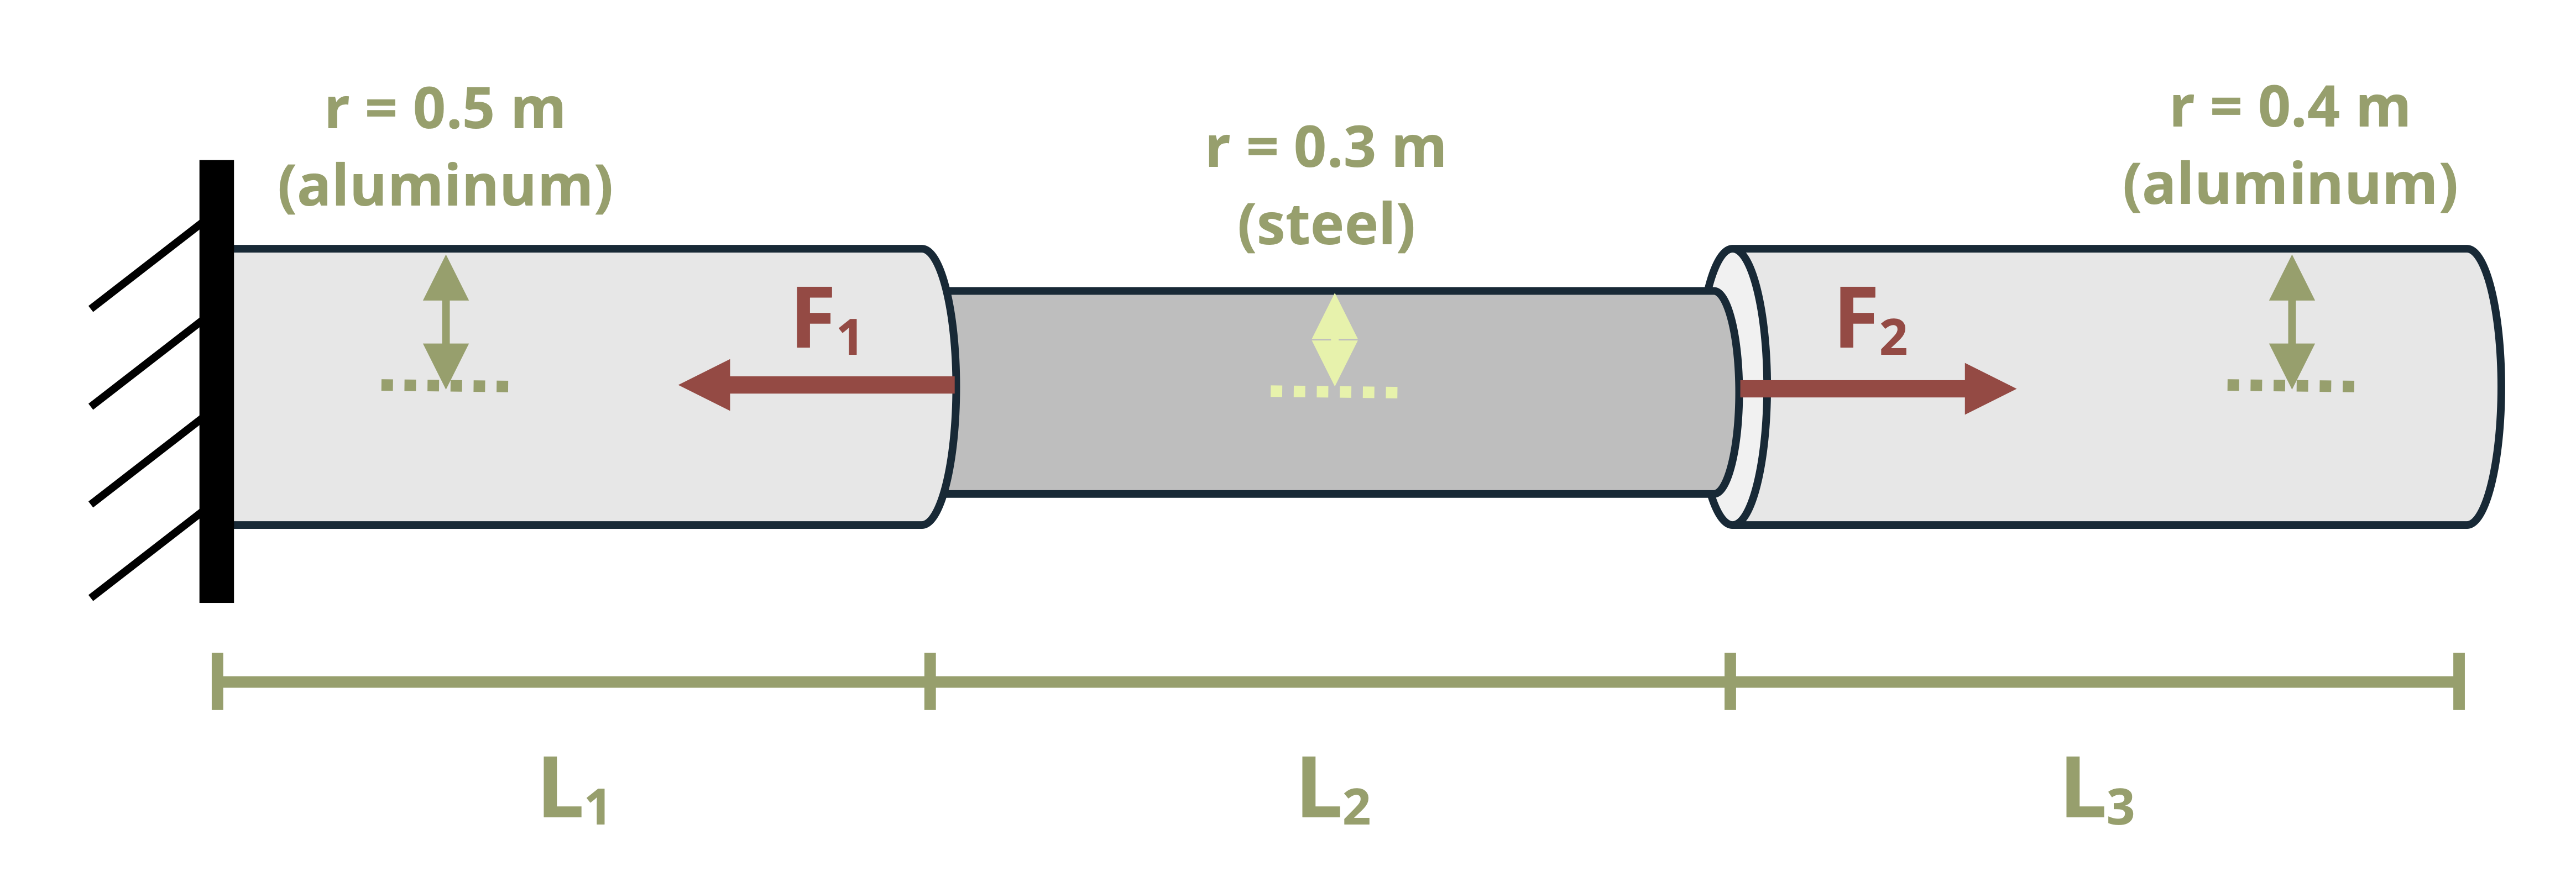
\includegraphics{images/184.png}

}

\caption{Figure 1: Two forces are applied to the system of cylinders.}

\end{figure}%

\begin{Shaded}
\begin{Highlighting}[]
\NormalTok{\#| standalone: true}
\NormalTok{\#| viewerHeight: 600}
\NormalTok{\#| components: [viewer]}

\NormalTok{from shiny import App, render, ui, reactive}
\NormalTok{import random}
\NormalTok{import asyncio}
\NormalTok{import io}
\NormalTok{import math}
\NormalTok{import string}
\NormalTok{from datetime import datetime}
\NormalTok{from pathlib import Path}

\NormalTok{def generate\_random\_letters(length):}
\NormalTok{    \# Generate a random string of letters of specified length}
\NormalTok{    return \textquotesingle{}\textquotesingle{}.join(random.choice(string.ascii\_lowercase) for \_ in range(length)) }

\NormalTok{problem\_ID="184"}
\NormalTok{F1=reactive.Value("\_\_")}
\NormalTok{F2=reactive.Value("\_\_")}
\NormalTok{L1=reactive.Value("\_\_")}
\NormalTok{L2=reactive.Value("\_\_")}
\NormalTok{L3=reactive.Value("\_\_")}
\NormalTok{Esteel = 210}
\NormalTok{Ealuminum = 70}

\NormalTok{attempts=["Timestamp,Attempt,Answer,Feedback\textbackslash{}n"]}

\NormalTok{app\_ui = ui.page\_fluid(}
\NormalTok{    ui.markdown("**Please enter your ID number from your instructor and click to generate your problem**"),}
\NormalTok{    ui.input\_text("ID","", placeholder="Enter ID Number Here"),}
\NormalTok{    ui.input\_action\_button("generate\_problem", "Generate Problem", class\_="btn{-}primary"),}
\NormalTok{    ui.markdown("**Problem Statement**"),}
\NormalTok{    ui.output\_ui("ui\_problem\_statement"),}
\NormalTok{    ui.input\_text("answer","Your Answer in units of micrometers", placeholder="Please enter your answer"),}
\NormalTok{    ui.input\_action\_button("submit", "Submit Answer", class\_="btn{-}primary"),}
\NormalTok{    ui.download\_button("download", "Download File to Submit", class\_="btn{-}success"),}
\NormalTok{)}

\NormalTok{def server(input, output, session):}
\NormalTok{    \# Initialize a counter for attempts}
\NormalTok{    attempt\_counter = reactive.Value(0)}

\NormalTok{    @output}
\NormalTok{    @render.ui}
\NormalTok{    def ui\_problem\_statement():}
\NormalTok{        return[ui.markdown(f"Two forces, F\textless{}sub\textgreater{}1\textless{}/sub\textgreater{} = \{F1()\} kN and F\textless{}sub\textgreater{}2\textless{}/sub\textgreater{} = \{F2()\} kN, are applied to the system of cylinders as shown. If L\textless{}sub\textgreater{}1\textless{}/sub\textgreater{} = \{L1()\} m, L\textless{}sub\textgreater{}2\textless{}/sub\textgreater{} = \{L2()\} m, and L\textless{}sub\textgreater{}3\textless{}/sub\textgreater{} = \{L3()\} m, what is the total change in length of the system? Assume E\textless{}sub\textgreater{}steel\textless{}/sub\textgreater{} = \{Esteel\} GPa and E\textless{}sub\textgreater{}aluminum\textless{}/sub\textgreater{} = \{Ealuminum\} GPa.")]}
    
\NormalTok{    @reactive.Effect}
\NormalTok{    @reactive.event(input.generate\_problem)}
\NormalTok{    def randomize\_vars():}
\NormalTok{        random.seed(input.ID())}
\NormalTok{        F1.set(random.randrange(100, 300, 1)/10)}
\NormalTok{        F2.set(round(F1()/1.5, 2))}
\NormalTok{        L1.set(random.randrange(20, 80, 1)/10)}
\NormalTok{        L2.set(round(L1()*0.6, 2))}
\NormalTok{        L3.set(round(L1()*0.8, 2))}
        
\NormalTok{    @reactive.Effect}
\NormalTok{    @reactive.event(input.submit)}
\NormalTok{    def \_():}
\NormalTok{        attempt\_counter.set(attempt\_counter() + 1)  \# Increment the attempt counter on each submission.}
       
\NormalTok{        instr= ((F2()*10**3*L2())/(math.pi*0.3**2*Esteel*10**9) + ((F2(){-}F1())*1000*L1())/(math.pi*0.5**2*Ealuminum*10**9))*1000000}
\NormalTok{        if math.isclose(float(input.answer()), instr, rel\_tol=0.01):}
\NormalTok{            check = "*Correct*"}
\NormalTok{            correct\_indicator = "JL"}
\NormalTok{        else:}
\NormalTok{            check = "*Not Correct.*"}
\NormalTok{            correct\_indicator = "JG"}

\NormalTok{        \# Generate random parts for the encoded attempt.}
\NormalTok{        random\_start = generate\_random\_letters(4)}
\NormalTok{        random\_middle = generate\_random\_letters(4)}
\NormalTok{        random\_end = generate\_random\_letters(4)}
\NormalTok{        encoded\_attempt = f"\{random\_start\}\{problem\_ID\}{-}\{random\_middle\}\{attempt\_counter()\}\{correct\_indicator\}{-}\{random\_end\}\{input.ID()\}"}

\NormalTok{        \# Store the most recent encoded attempt in a reactive value so it persists across submissions}
\NormalTok{        session.encoded\_attempt = reactive.Value(encoded\_attempt)}

\NormalTok{        \# Append the attempt data to the attempts list without the encoded attempt}
\NormalTok{        attempts.append(f"\{datetime.now()\}, \{attempt\_counter()\}, \{input.answer()\}, \{check\}\textbackslash{}n")}

\NormalTok{        \# Show feedback to the user.}
\NormalTok{        feedback = ui.markdown(f"Your answer of \{input.answer()\} is \{check\}.")}
\NormalTok{        m = ui.modal(}
\NormalTok{            feedback,}
\NormalTok{            title="Feedback",}
\NormalTok{            easy\_close=True}
\NormalTok{        )}
\NormalTok{        ui.modal\_show(m)}

\NormalTok{    @session.download(filename=lambda: f"Problem\_Log{-}\{problem\_ID\}{-}\{input.ID()\}.csv")}
\NormalTok{    async def download():}
\NormalTok{        \# Start the CSV with the encoded attempt (without label)}
\NormalTok{        final\_encoded = session.encoded\_attempt() if session.encoded\_attempt is not None else "No attempts"}
\NormalTok{        yield f"\{final\_encoded\}\textbackslash{}n\textbackslash{}n"}
        
\NormalTok{        \# Write the header for the remaining CSV data once}
\NormalTok{        yield "Timestamp,Attempt,Answer,Feedback\textbackslash{}n"}
        
\NormalTok{        \# Write the attempts data, ensure that the header from the attempts list is not written again}
\NormalTok{        for attempt in attempts[1:]:  \# Skip the first element which is the header}
\NormalTok{            await asyncio.sleep(0.25)  \# This delay may not be necessary; adjust as needed}
\NormalTok{            yield attempt}

\NormalTok{\# App installation}
\NormalTok{app = App(app\_ui, server)}
\end{Highlighting}
\end{Shaded}

\chapter*{Problem 5.13}\label{problem-5.13}
\addcontentsline{toc}{chapter}{Problem 5.13}

\markboth{Problem 5.13}{Problem 5.13}

This is a dynamic rendering of the problem with dynamic variables based
on the username entered.

\section*{Problem Image}\label{problem-image-43}
\addcontentsline{toc}{section}{Problem Image}

\markright{Problem Image}

\begin{figure}[H]

{\centering 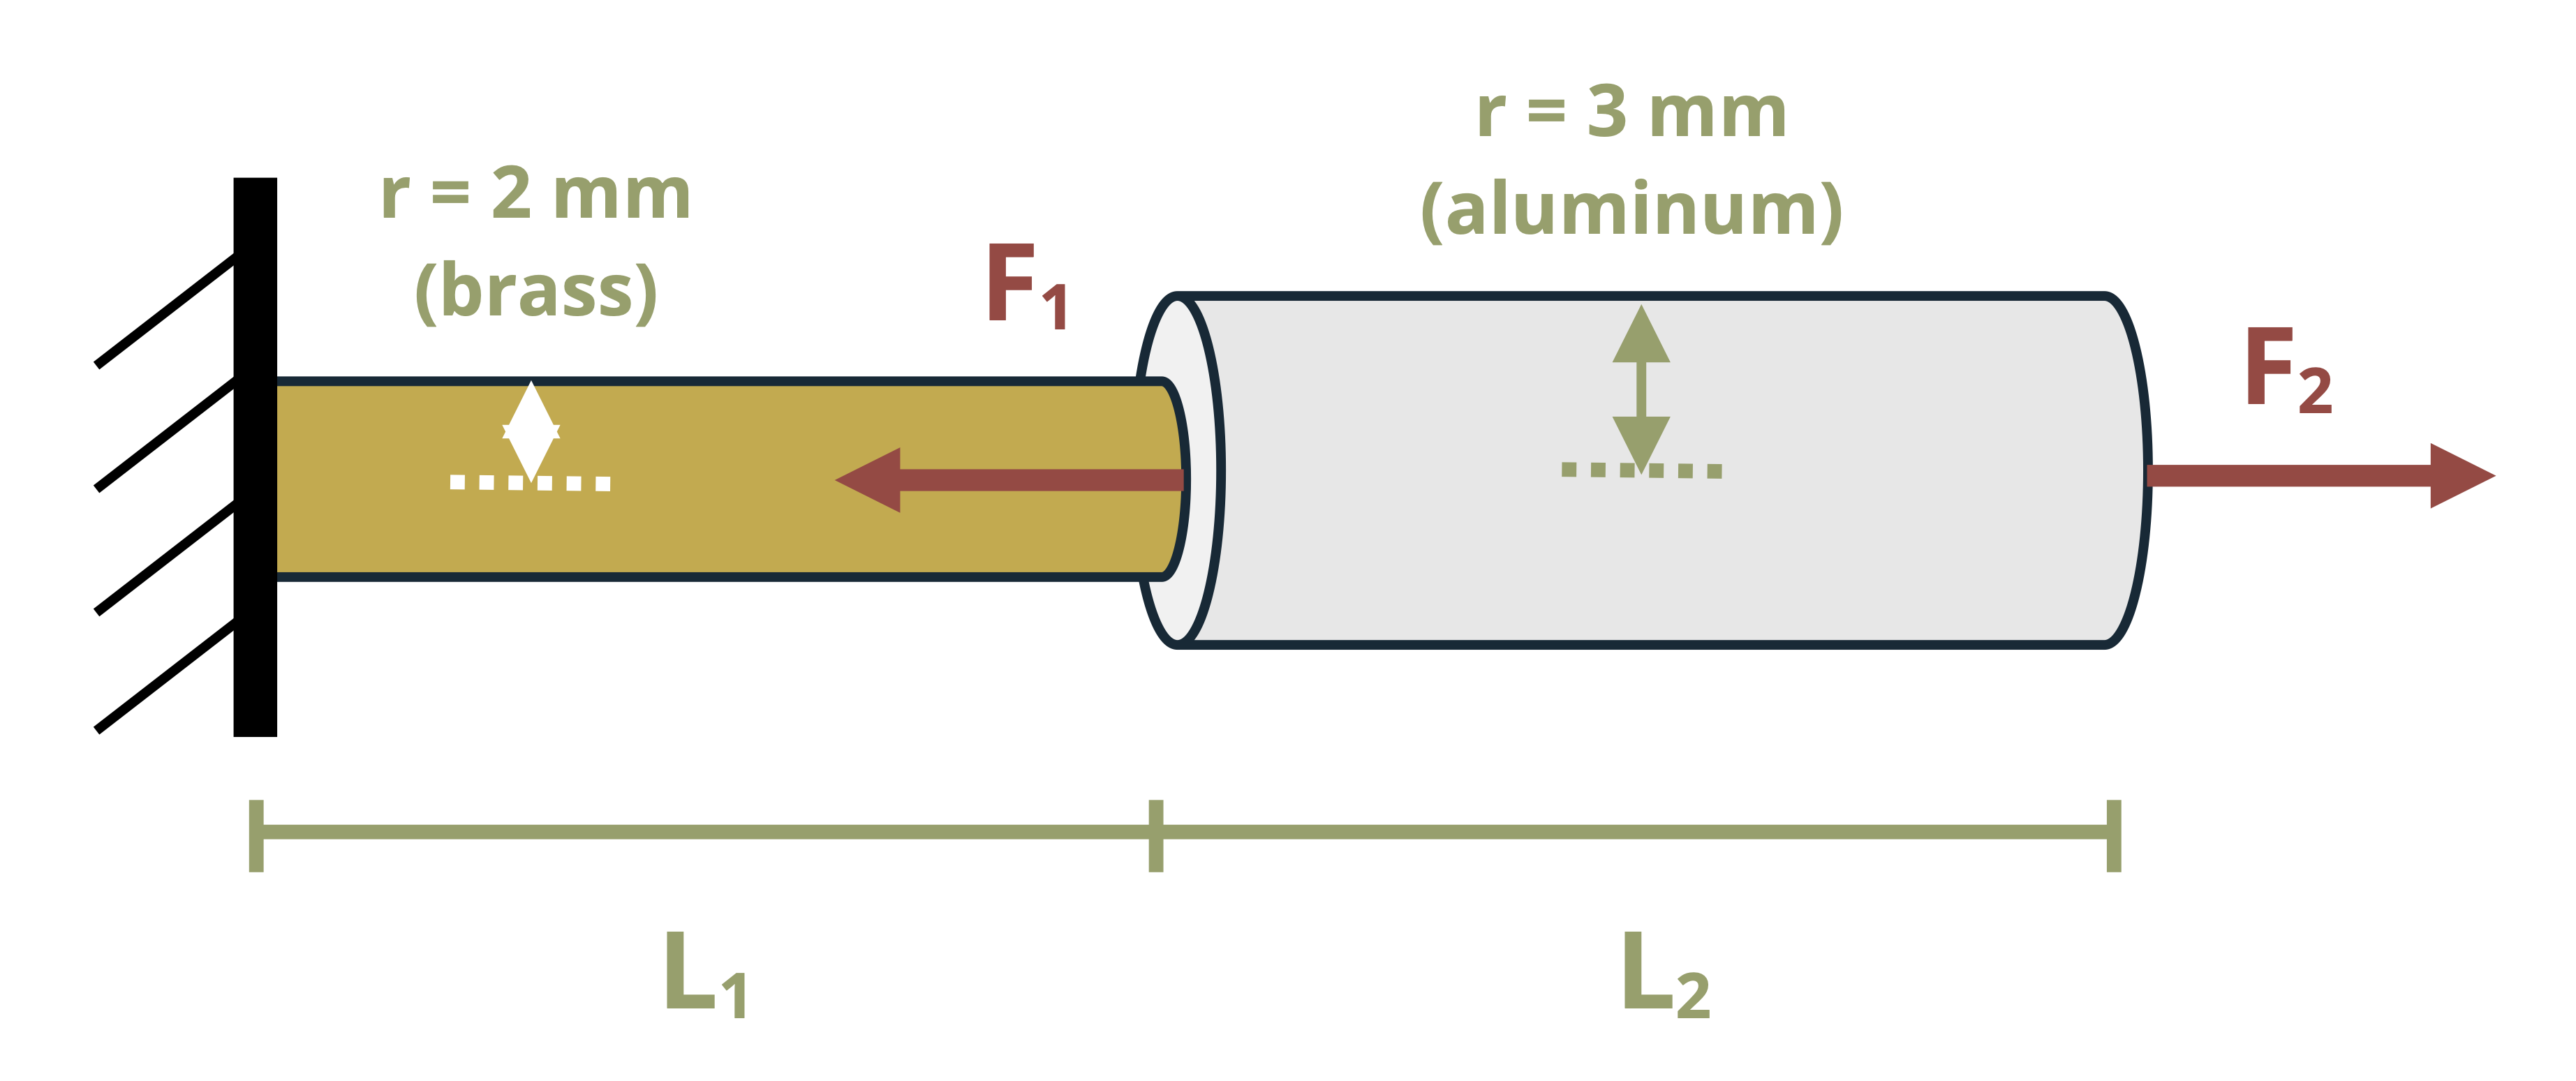
\includegraphics{images/185.png}

}

\caption{Figure 1: Two forces are applied to the system of cylinders.}

\end{figure}%

\begin{Shaded}
\begin{Highlighting}[]
\NormalTok{\#| standalone: true}
\NormalTok{\#| viewerHeight: 600}
\NormalTok{\#| components: [viewer]}

\NormalTok{from shiny import App, render, ui, reactive}
\NormalTok{import random}
\NormalTok{import asyncio}
\NormalTok{import io}
\NormalTok{import math}
\NormalTok{import string}
\NormalTok{from datetime import datetime}
\NormalTok{from pathlib import Path}

\NormalTok{def generate\_random\_letters(length):}
\NormalTok{    \# Generate a random string of letters of specified length}
\NormalTok{    return \textquotesingle{}\textquotesingle{}.join(random.choice(string.ascii\_lowercase) for \_ in range(length))}

\NormalTok{problem\_ID="185"}
\NormalTok{F1=reactive.Value("\_\_")}
\NormalTok{F2=reactive.Value("\_\_")}
\NormalTok{L1=reactive.Value("\_\_")}
\NormalTok{L2=reactive.Value("\_\_")}
\NormalTok{Ebrass = 100}
\NormalTok{Ealuminum = 70}

\NormalTok{attempts=["Timestamp,Attempt,Answer,Feedback\textbackslash{}n"]}

\NormalTok{app\_ui = ui.page\_fluid(}
\NormalTok{    ui.markdown("**Please enter your ID number from your instructor and click to generate your problem**"),}
\NormalTok{    ui.input\_text("ID","", placeholder="Enter ID Number Here"),}
\NormalTok{    ui.input\_action\_button("generate\_problem", "Generate Problem", class\_="btn{-}primary"),}
\NormalTok{    ui.markdown("**Problem Statement**"),}
\NormalTok{    ui.output\_ui("ui\_problem\_statement"),}
\NormalTok{    ui.input\_text("answer","Your Answer in units of mm", placeholder="Please enter your answer"),}
\NormalTok{    ui.input\_action\_button("submit", "Submit Answer", class\_="btn{-}primary"),}
\NormalTok{    ui.download\_button("download", "Download File to Submit", class\_="btn{-}success"),}
\NormalTok{)}

\NormalTok{def server(input, output, session):}
\NormalTok{    \# Initialize a counter for attempts}
\NormalTok{    attempt\_counter = reactive.Value(0)}

\NormalTok{    @output}
\NormalTok{    @render.ui}
\NormalTok{    def ui\_problem\_statement():}
\NormalTok{        return[ui.markdown(f"Two forces, F\textless{}sub\textgreater{}1\textless{}/sub\textgreater{} = \{F1()\} kN and F\textless{}sub\textgreater{}2\textless{}/sub\textgreater{} = \{F2()\} kN, are applied to the system of cylinders as shown. If L\textless{}sub\textgreater{}1\textless{}/sub\textgreater{} = \{L1()\} mm and L\textless{}sub\textgreater{}2\textless{}/sub\textgreater{} = \{L2()\} mm, what is the total change in length of the system. Assume E\textless{}sub\textgreater{}brass\textless{}/sub\textgreater{} = \{Ebrass\} GPa and E\textless{}sub\textgreater{}aluminum\textless{}/sub\textgreater{} = \{Ealuminum\} GPa.")]}
    
\NormalTok{    @reactive.Effect}
\NormalTok{    @reactive.event(input.generate\_problem)}
\NormalTok{    def randomize\_vars():}
\NormalTok{        random.seed(input.ID())}
\NormalTok{        F1.set(random.randrange(10, 100, 1)/10)}
\NormalTok{        F2.set(round(F1()*2, 2))}
\NormalTok{        L1.set(random.randrange(50, 150, 1))}
\NormalTok{        L2.set(round(L1()*1.5))}
        
\NormalTok{    @reactive.Effect}
\NormalTok{    @reactive.event(input.submit)}
\NormalTok{    def \_():}
\NormalTok{        attempt\_counter.set(attempt\_counter() + 1)  \# Increment the attempt counter on each submission.}
\NormalTok{        instr= (((F2(){-}F1())*L1())/(math.pi*.002**2*Ebrass*10**6)) + (F2()*L2())/(math.pi*.003**2*Ealuminum*10**6)}
\NormalTok{        if math.isclose(float(input.answer()), instr, rel\_tol=0.01):}
\NormalTok{            check = "*Correct*"}
\NormalTok{            correct\_indicator = "JL"}
\NormalTok{        else:}
\NormalTok{            check = "*Not Correct.*"}
\NormalTok{            correct\_indicator = "JG"}

\NormalTok{        \# Generate random parts for the encoded attempt.}
\NormalTok{        random\_start = generate\_random\_letters(4)}
\NormalTok{        random\_middle = generate\_random\_letters(4)}
\NormalTok{        random\_end = generate\_random\_letters(4)}
\NormalTok{        encoded\_attempt = f"\{random\_start\}\{problem\_ID\}{-}\{random\_middle\}\{attempt\_counter()\}\{correct\_indicator\}{-}\{random\_end\}\{input.ID()\}"}

\NormalTok{        \# Store the most recent encoded attempt in a reactive value so it persists across submissions}
\NormalTok{        session.encoded\_attempt = reactive.Value(encoded\_attempt)}

\NormalTok{        \# Append the attempt data to the attempts list without the encoded attempt}
\NormalTok{        attempts.append(f"\{datetime.now()\}, \{attempt\_counter()\}, \{input.answer()\}, \{check\}\textbackslash{}n")}

\NormalTok{        \# Show feedback to the user.}
\NormalTok{        feedback = ui.markdown(f"Your answer of \{input.answer()\} is \{check\}.")}
\NormalTok{        m = ui.modal(}
\NormalTok{            feedback,}
\NormalTok{            title="Feedback",}
\NormalTok{            easy\_close=True}
\NormalTok{        )}
\NormalTok{        ui.modal\_show(m)}

\NormalTok{    @session.download(filename=lambda: f"Problem\_Log{-}\{problem\_ID\}{-}\{input.ID()\}.csv")}
\NormalTok{    async def download():}
\NormalTok{        \# Start the CSV with the encoded attempt (without label)}
\NormalTok{        final\_encoded = session.encoded\_attempt() if session.encoded\_attempt is not None else "No attempts"}
\NormalTok{        yield f"\{final\_encoded\}\textbackslash{}n\textbackslash{}n"}
        
\NormalTok{        \# Write the header for the remaining CSV data once}
\NormalTok{        yield "Timestamp,Attempt,Answer,Feedback\textbackslash{}n"}
        
\NormalTok{        \# Write the attempts data, ensure that the header from the attempts list is not written again}
\NormalTok{        for attempt in attempts[1:]:  \# Skip the first element which is the header}
\NormalTok{            await asyncio.sleep(0.25)  \# This delay may not be necessary; adjust as needed}
\NormalTok{            yield attempt}

\NormalTok{\# App installation}
\NormalTok{app = App(app\_ui, server)}
\end{Highlighting}
\end{Shaded}

\chapter*{Problem 5.14}\label{problem-5.14}
\addcontentsline{toc}{chapter}{Problem 5.14}

\markboth{Problem 5.14}{Problem 5.14}

This is a dynamic rendering of the problem with dynamic variables based
on the username entered.

\section*{Problem Image}\label{problem-image-44}
\addcontentsline{toc}{section}{Problem Image}

\markright{Problem Image}

\begin{figure}[H]

{\centering 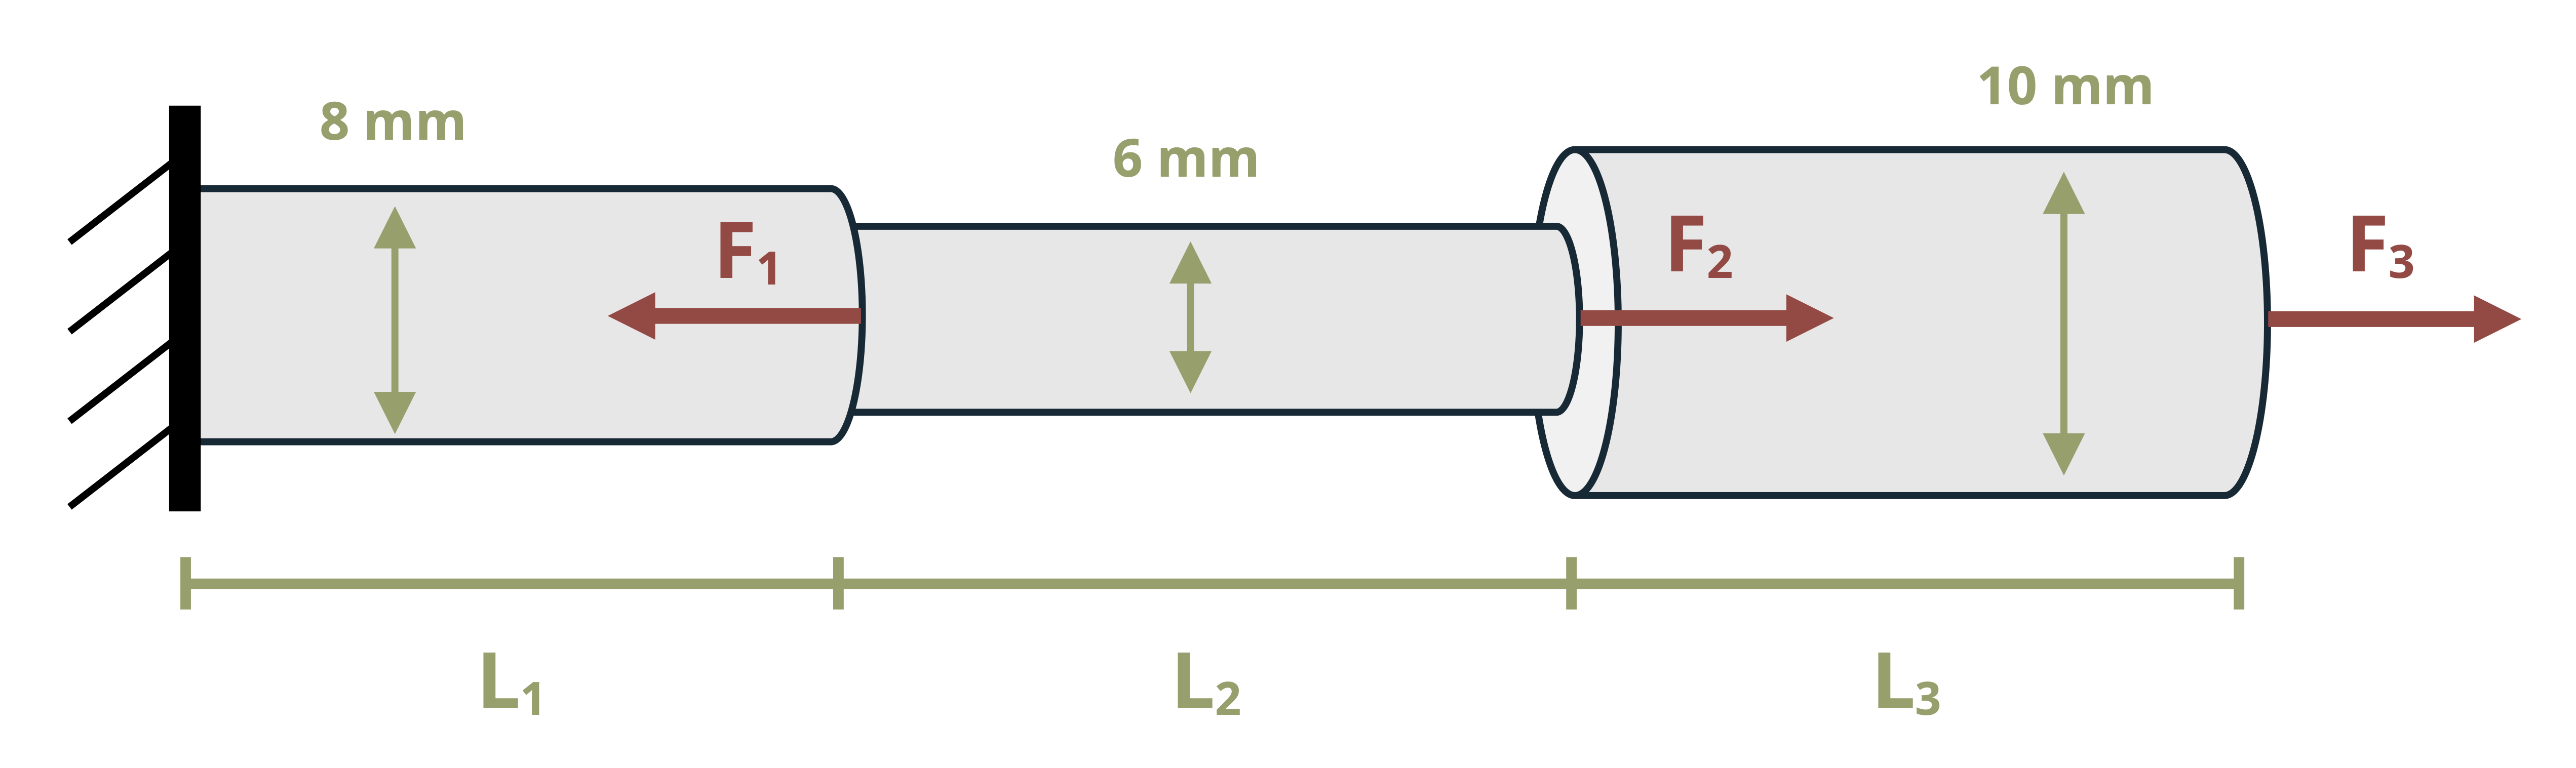
\includegraphics{images/186.png}

}

\caption{Figure 1: A series of solid circular steel bars are loaded with
three loads.}

\end{figure}%

\begin{Shaded}
\begin{Highlighting}[]
\NormalTok{\#| standalone: true}
\NormalTok{\#| viewerHeight: 600}
\NormalTok{\#| components: [viewer]}

\NormalTok{from shiny import App, render, ui, reactive}
\NormalTok{import random}
\NormalTok{import asyncio}
\NormalTok{import io}
\NormalTok{import math}
\NormalTok{import string}
\NormalTok{from datetime import datetime}
\NormalTok{from pathlib import Path}

\NormalTok{def generate\_random\_letters(length):}
\NormalTok{    \# Generate a random string of letters of specified length}
\NormalTok{    return \textquotesingle{}\textquotesingle{}.join(random.choice(string.ascii\_lowercase) for \_ in range(length))}

\NormalTok{problem\_ID="186"}
\NormalTok{F1=reactive.Value("\_\_")}
\NormalTok{F2=reactive.Value("\_\_")}
\NormalTok{F3=reactive.Value("\_\_")}
\NormalTok{L1=reactive.Value("\_\_")}
\NormalTok{L2=reactive.Value("\_\_")}
\NormalTok{L3=reactive.Value("\_\_")}

\NormalTok{attempts=["Timestamp,Attempt,Answer,Feedback\textbackslash{}n"]}

\NormalTok{app\_ui = ui.page\_fluid(}
\NormalTok{    ui.markdown("**Please enter your ID number from your instructor and click to generate your problem**"),}
\NormalTok{    ui.input\_text("ID","", placeholder="Enter ID Number Here"),}
\NormalTok{    ui.input\_action\_button("generate\_problem", "Generate Problem", class\_="btn{-}primary"),}
\NormalTok{    ui.markdown("**Problem Statement**"),}
\NormalTok{    ui.output\_ui("ui\_problem\_statement"),}
\NormalTok{    ui.input\_text("answer","Your Answer in units of mm", placeholder="Please enter your answer"),}
\NormalTok{    ui.input\_action\_button("submit", "Submit Answer", class\_="btn{-}primary"),}
\NormalTok{    ui.download\_button("download", "Download File to Submit", class\_="btn{-}success"),}
\NormalTok{)}

\NormalTok{def server(input, output, session):}
\NormalTok{    \# Initialize a counter for attempts}
\NormalTok{    attempt\_counter = reactive.Value(0)}

\NormalTok{    @output}
\NormalTok{    @render.ui}
\NormalTok{    def ui\_problem\_statement():}
\NormalTok{        return[ui.markdown(f"A series of solid circular steel bars are loaded as shown, where F\textless{}sub\textgreater{}1\textless{}/sub\textgreater{} = \{F1()\} N, F\textless{}sub\textgreater{}2\textless{}/sub\textgreater{} = \{F2()\} N, and F\textless{}sub\textgreater{}3\textless{}/sub\textgreater{} = \{F3()\} N. If lengths L\textless{}sub\textgreater{}1\textless{}/sub\textgreater{} = L\textless{}sub\textgreater{}2\textless{}/sub\textgreater{} = \{L1()\} cm and L\textless{}sub\textgreater{}3\textless{}/sub\textgreater{} = \{L3()\} cm, determine the total change in length of the system. Assume E\textless{}sub\textgreater{}steel\textless{}/sub\textgreater{} = 210 GPa.")]}
    
\NormalTok{    @reactive.Effect}
\NormalTok{    @reactive.event(input.generate\_problem)}
\NormalTok{    def randomize\_vars():}
\NormalTok{        random.seed(input.ID())}
\NormalTok{        F1.set(random.randrange(20, 100, 1))}
\NormalTok{        F2.set(random.randrange(20, 100, 1))}
\NormalTok{        F3.set(random.randrange(20, 100, 1))}
\NormalTok{        L1.set(random.randrange(20, 60, 1))}
\NormalTok{        L2.set(L1())}
\NormalTok{        L3.set(round(L1()*1.25))}
        
\NormalTok{    @reactive.Effect}
\NormalTok{    @reactive.event(input.submit)}
\NormalTok{    def \_():}
\NormalTok{        attempt\_counter.set(attempt\_counter() + 1)  \# Increment the attempt counter on each submission.}
\NormalTok{        R = F2()+F3(){-}F1()}
\NormalTok{        FBC = F1()+R}
\NormalTok{        dAB = R*L1()/100/(210*10**9*0.004**2*math.pi)}
\NormalTok{        dBC = FBC*L2()/100/(210*10**9*0.003**2*math.pi)}
\NormalTok{        dCD = F3()*L3()/100/(210*10**9*0.005**2*math.pi)}
\NormalTok{        instr= abs((dAB+dBC+dCD)*10**3)}
\NormalTok{        if math.isclose(float(input.answer()), instr, rel\_tol=0.01):}
\NormalTok{            check = "*Correct*"}
\NormalTok{            correct\_indicator = "JL"}
\NormalTok{        else:}
\NormalTok{            check = "*Not Correct.*"}
\NormalTok{            correct\_indicator = "JG"}

\NormalTok{        \# Generate random parts for the encoded attempt.}
\NormalTok{        random\_start = generate\_random\_letters(4)}
\NormalTok{        random\_middle = generate\_random\_letters(4)}
\NormalTok{        random\_end = generate\_random\_letters(4)}
\NormalTok{        encoded\_attempt = f"\{random\_start\}\{problem\_ID\}{-}\{random\_middle\}\{attempt\_counter()\}\{correct\_indicator\}{-}\{random\_end\}\{input.ID()\}"}

\NormalTok{        \# Store the most recent encoded attempt in a reactive value so it persists across submissions}
\NormalTok{        session.encoded\_attempt = reactive.Value(encoded\_attempt)}

\NormalTok{        \# Append the attempt data to the attempts list without the encoded attempt}
\NormalTok{        attempts.append(f"\{datetime.now()\}, \{attempt\_counter()\}, \{input.answer()\}, \{check\}\textbackslash{}n")}

\NormalTok{        \# Show feedback to the user.}
\NormalTok{        feedback = ui.markdown(f"Your answer of \{input.answer()\} is \{check\}.")}
\NormalTok{        m = ui.modal(}
\NormalTok{            feedback,}
\NormalTok{            title="Feedback",}
\NormalTok{            easy\_close=True}
\NormalTok{        )}
\NormalTok{        ui.modal\_show(m)}

\NormalTok{    @session.download(filename=lambda: f"Problem\_Log{-}\{problem\_ID\}{-}\{input.ID()\}.csv")}
\NormalTok{    async def download():}
\NormalTok{        \# Start the CSV with the encoded attempt (without label)}
\NormalTok{        final\_encoded = session.encoded\_attempt() if session.encoded\_attempt is not None else "No attempts"}
\NormalTok{        yield f"\{final\_encoded\}\textbackslash{}n\textbackslash{}n"}
        
\NormalTok{        \# Write the header for the remaining CSV data once}
\NormalTok{        yield "Timestamp,Attempt,Answer,Feedback\textbackslash{}n"}
        
\NormalTok{        \# Write the attempts data, ensure that the header from the attempts list is not written again}
\NormalTok{        for attempt in attempts[1:]:  \# Skip the first element which is the header}
\NormalTok{            await asyncio.sleep(0.25)  \# This delay may not be necessary; adjust as needed}
\NormalTok{            yield attempt}

\NormalTok{\# App installation}
\NormalTok{app = App(app\_ui, server)}
\end{Highlighting}
\end{Shaded}

\chapter*{Problem 5.15}\label{problem-5.15}
\addcontentsline{toc}{chapter}{Problem 5.15}

\markboth{Problem 5.15}{Problem 5.15}

This is a dynamic rendering of the problem with dynamic variables based
on the username entered.

\section*{Problem Image}\label{problem-image-45}
\addcontentsline{toc}{section}{Problem Image}

\markright{Problem Image}

\begin{figure}[H]

{\centering 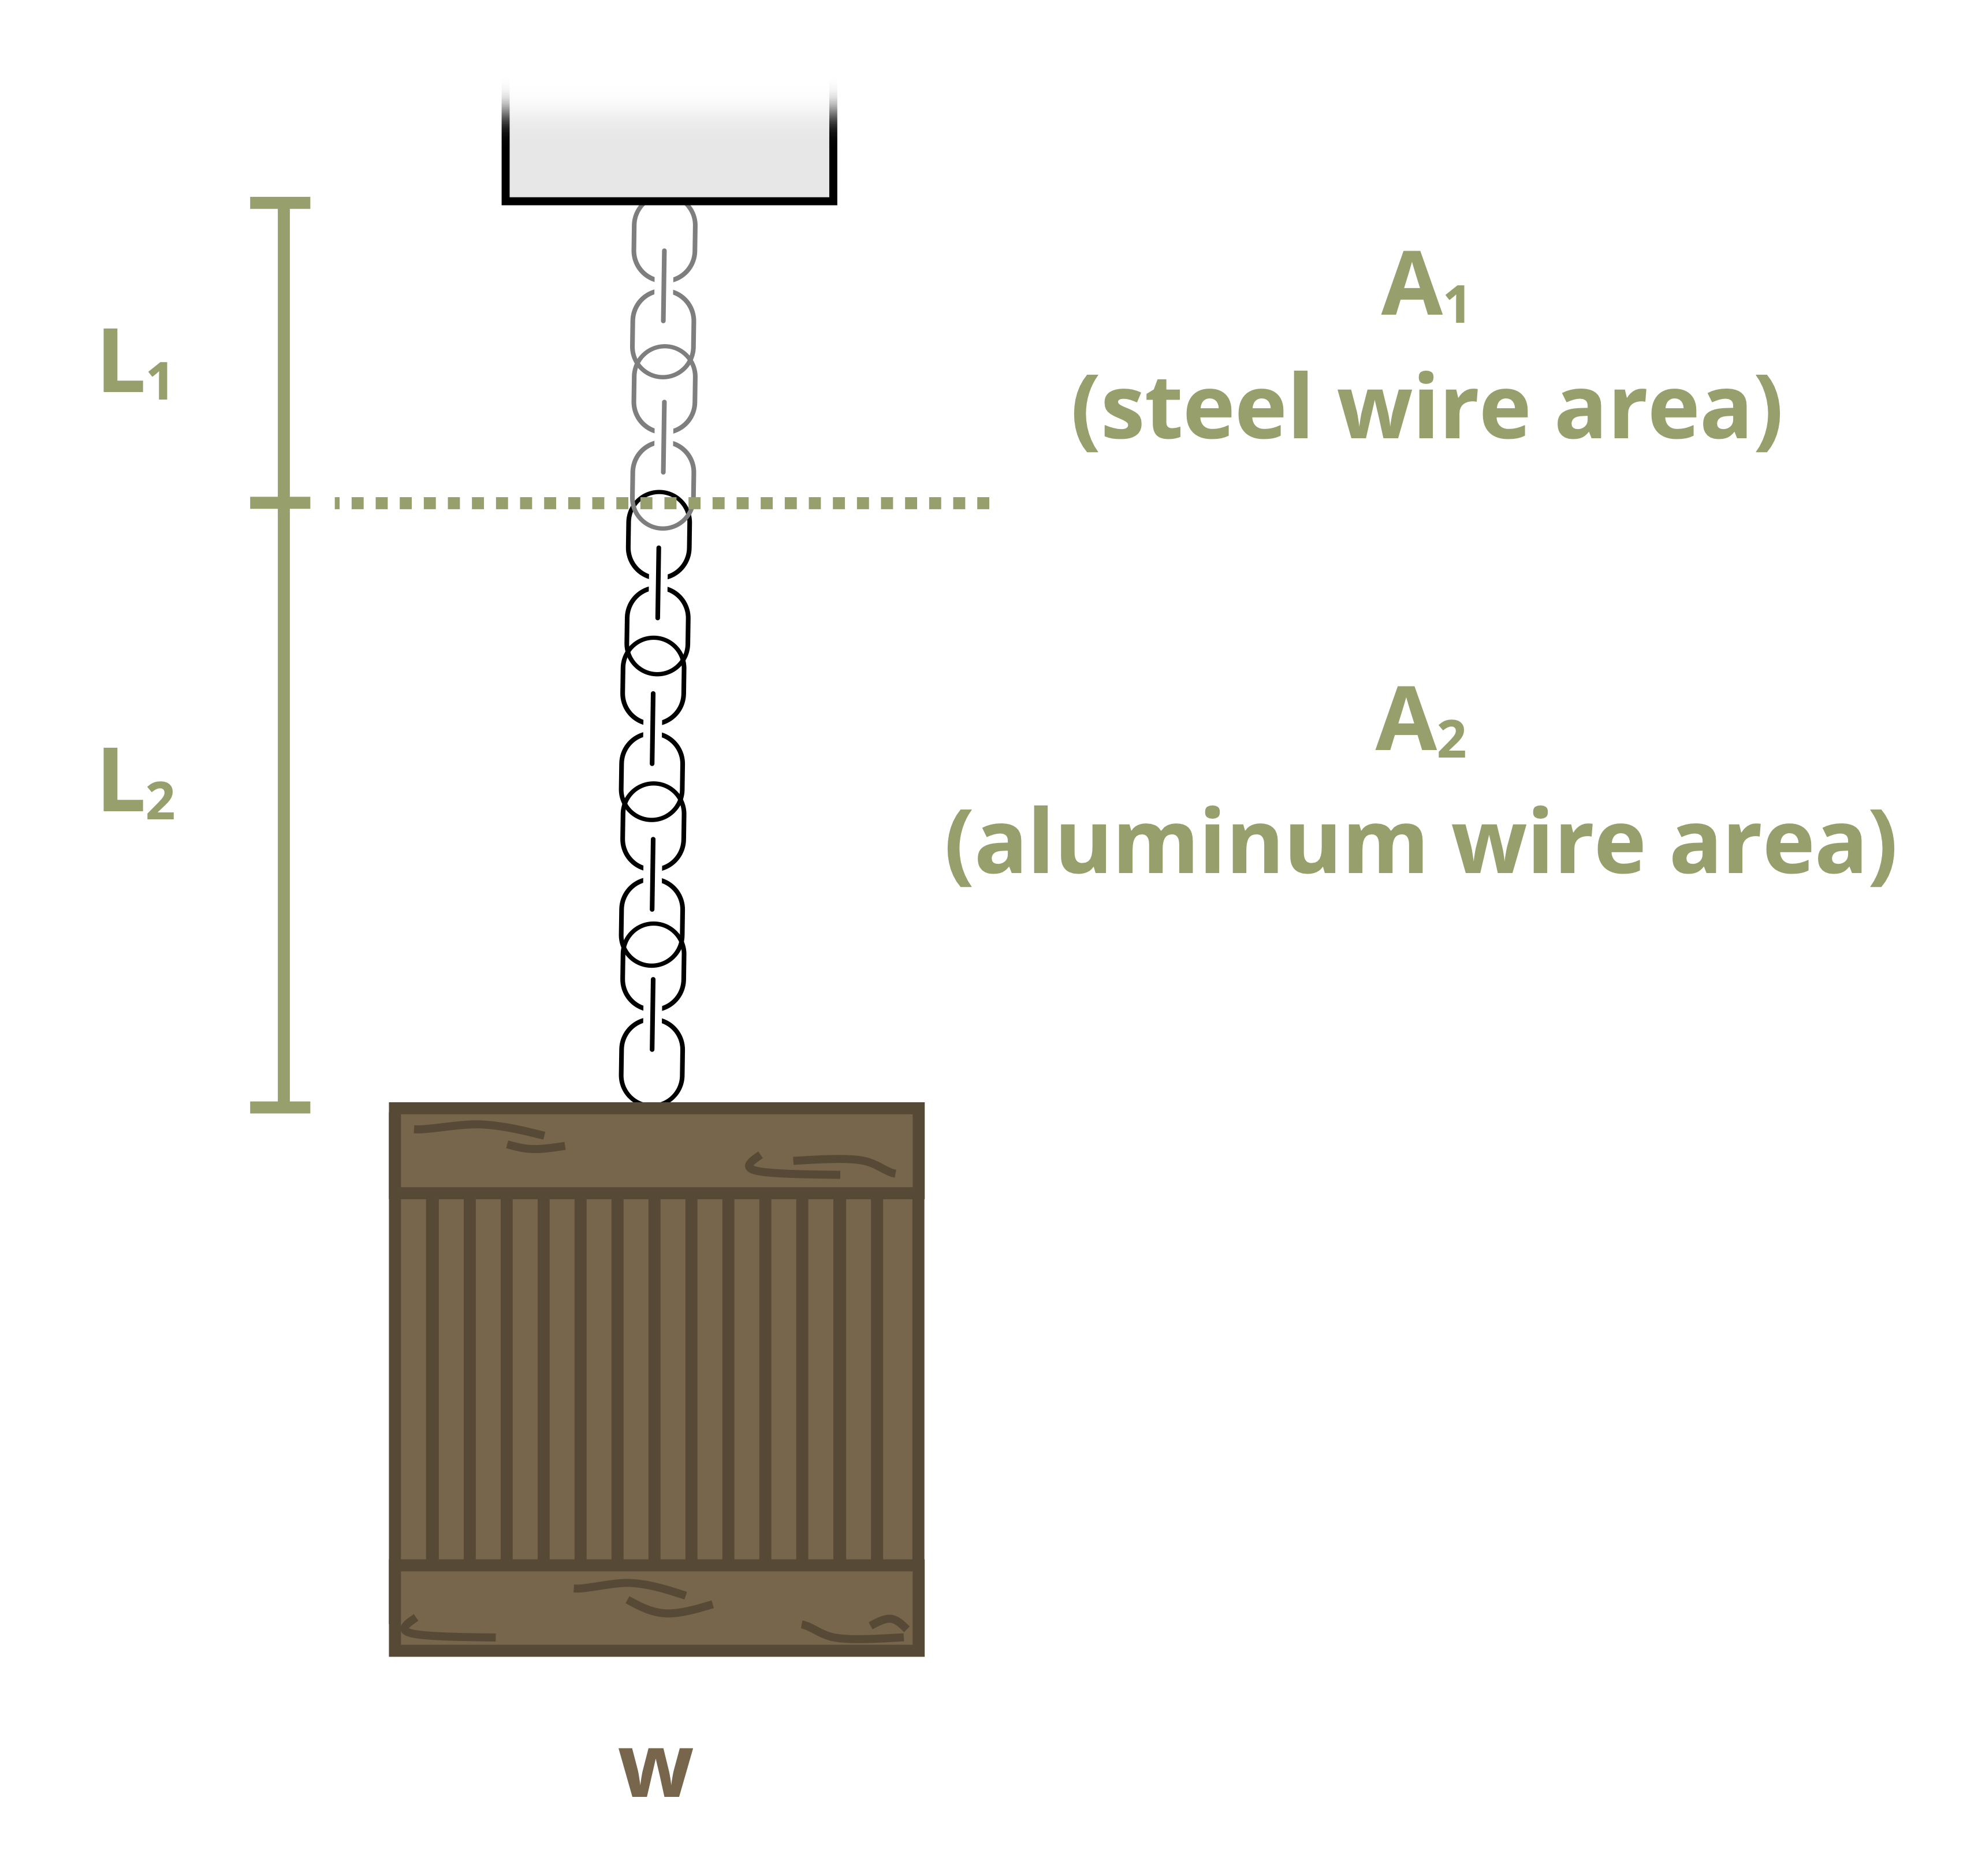
\includegraphics{images/187.png}

}

\caption{Figure 1: A crate is attached to a cable made from steel and
aluminum.}

\end{figure}%

\begin{Shaded}
\begin{Highlighting}[]
\NormalTok{\#| standalone: true}
\NormalTok{\#| viewerHeight: 600}
\NormalTok{\#| components: [viewer]}

\NormalTok{from shiny import App, render, ui, reactive}
\NormalTok{import random}
\NormalTok{import asyncio}
\NormalTok{import io}
\NormalTok{import math}
\NormalTok{import string}
\NormalTok{from datetime import datetime}
\NormalTok{from pathlib import Path}

\NormalTok{def generate\_random\_letters(length):}
\NormalTok{    \# Generate a random string of letters of specified length}
\NormalTok{    return \textquotesingle{}\textquotesingle{}.join(random.choice(string.ascii\_lowercase) for \_ in range(length)) }

\NormalTok{problem\_ID="187"}
\NormalTok{W=reactive.Value("\_\_")}
\NormalTok{L1=reactive.Value("\_\_")}
\NormalTok{L2=reactive.Value("\_\_")}
\NormalTok{A1=reactive.Value("\_\_")}
\NormalTok{A2=reactive.Value("\_\_")}
\NormalTok{Esteel = 29000}
\NormalTok{Ealuminum = 10000}

\NormalTok{attempts=["Timestamp,Attempt,Answer,Feedback\textbackslash{}n"]}

\NormalTok{app\_ui = ui.page\_fluid(}
\NormalTok{    ui.markdown("**Please enter your ID number from your instructor and click to generate your problem**"),}
\NormalTok{    ui.input\_text("ID","", placeholder="Enter ID Number Here"),}
\NormalTok{    ui.input\_action\_button("generate\_problem", "Generate Problem", class\_="btn{-}primary"),}
\NormalTok{    ui.markdown("**Problem Statement**"),}
\NormalTok{    ui.output\_ui("ui\_problem\_statement"),}
\NormalTok{    ui.input\_text("answer","Your Answer in units of inches", placeholder="Please enter your answer"),}
\NormalTok{    ui.input\_action\_button("submit", "Submit Answer", class\_="btn{-}primary"),}
\NormalTok{    ui.download\_button("download", "Download File to Submit", class\_="btn{-}success"),}
\NormalTok{)}

\NormalTok{def server(input, output, session):}
\NormalTok{    \# Initialize a counter for attempts}
\NormalTok{    attempt\_counter = reactive.Value(0)}

\NormalTok{    @output}
\NormalTok{    @render.ui}
\NormalTok{    def ui\_problem\_statement():}
\NormalTok{        return[ui.markdown(f"A crate weight W = \{W()\} lb is attached to a cable constructed from steel of length L\textless{}sub\textgreater{}1\textless{}/sub\textgreater{} = \{L1()\} in. and Area A\textless{}sub\textgreater{}1\textless{}/sub\textgreater{} = \{A1()\} in.\textless{}sup\textgreater{}2\textless{}/sup\textgreater{} and aluminum of length L\textless{}sub\textgreater{}2\textless{}/sub\textgreater{} = \{L2()\} in. and area A\textless{}sub\textgreater{}2\textless{}/sub\textgreater{} = \{A2()\} in.\textless{}sup\textgreater{}2\textless{}/sup\textgreater{}. What is the total deflection of the crate after it is attached to the wire? Assume E\textless{}sub\textgreater{}steel\textless{}/sub\textgreater{} = \{Esteel\} ksi and E\textless{}sub\textgreater{}aluminum\textless{}/sub\textgreater{} = \{Ealuminum\} ksi. Neglect the weight of the wires.")]}
    
\NormalTok{    @reactive.Effect}
\NormalTok{    @reactive.event(input.generate\_problem)}
\NormalTok{    def randomize\_vars():}
\NormalTok{        random.seed(input.ID())}
\NormalTok{        W.set(random.randrange(50, 250, 1))}
\NormalTok{        L1.set(random.randrange(10, 30, 1))}
\NormalTok{        L2.set(round(L1()*2, 2))}
\NormalTok{        A1.set(random.randrange(1, 5, 1)/100)}
\NormalTok{        A2.set(random.randrange(1, 5, 1)/100)}
        
\NormalTok{    @reactive.Effect}
\NormalTok{    @reactive.event(input.submit)}
\NormalTok{    def \_():}
\NormalTok{        attempt\_counter.set(attempt\_counter() + 1)  \# Increment the attempt counter on each submission.}
        
\NormalTok{        instr=(W()*L1()/(A1()*Esteel*1000) + (W()*L2()/(A2()*Ealuminum*1000)))}
\NormalTok{        if math.isclose(float(input.answer()), instr, rel\_tol=0.01):}
\NormalTok{            check = "*Correct*"}
\NormalTok{            correct\_indicator = "JL"}
\NormalTok{        else:}
\NormalTok{            check = "*Not Correct.*"}
\NormalTok{            correct\_indicator = "JG"}

\NormalTok{        \# Generate random parts for the encoded attempt.}
\NormalTok{        random\_start = generate\_random\_letters(4)}
\NormalTok{        random\_middle = generate\_random\_letters(4)}
\NormalTok{        random\_end = generate\_random\_letters(4)}
\NormalTok{        encoded\_attempt = f"\{random\_start\}\{problem\_ID\}{-}\{random\_middle\}\{attempt\_counter()\}\{correct\_indicator\}{-}\{random\_end\}\{input.ID()\}"}

\NormalTok{        \# Store the most recent encoded attempt in a reactive value so it persists across submissions}
\NormalTok{        session.encoded\_attempt = reactive.Value(encoded\_attempt)}

\NormalTok{        \# Append the attempt data to the attempts list without the encoded attempt}
\NormalTok{        attempts.append(f"\{datetime.now()\}, \{attempt\_counter()\}, \{input.answer()\}, \{check\}\textbackslash{}n")}

\NormalTok{        \# Show feedback to the user.}
\NormalTok{        feedback = ui.markdown(f"Your answer of \{input.answer()\} is \{check\}.")}
\NormalTok{        m = ui.modal(}
\NormalTok{            feedback,}
\NormalTok{            title="Feedback",}
\NormalTok{            easy\_close=True}
\NormalTok{        )}
\NormalTok{        ui.modal\_show(m)}

\NormalTok{    @session.download(filename=lambda: f"Problem\_Log{-}\{problem\_ID\}{-}\{input.ID()\}.csv")}
\NormalTok{    async def download():}
\NormalTok{        \# Start the CSV with the encoded attempt (without label)}
\NormalTok{        final\_encoded = session.encoded\_attempt() if session.encoded\_attempt is not None else "No attempts"}
\NormalTok{        yield f"\{final\_encoded\}\textbackslash{}n\textbackslash{}n"}
        
\NormalTok{        \# Write the header for the remaining CSV data once}
\NormalTok{        yield "Timestamp,Attempt,Answer,Feedback\textbackslash{}n"}
        
\NormalTok{        \# Write the attempts data, ensure that the header from the attempts list is not written again}
\NormalTok{        for attempt in attempts[1:]:  \# Skip the first element which is the header}
\NormalTok{            await asyncio.sleep(0.25)  \# This delay may not be necessary; adjust as needed}
\NormalTok{            yield attempt}

\NormalTok{\# App installation}
\NormalTok{app = App(app\_ui, server)}
\end{Highlighting}
\end{Shaded}

\chapter*{Problem 5.27}\label{problem-5.27}
\addcontentsline{toc}{chapter}{Problem 5.27}

\markboth{Problem 5.27}{Problem 5.27}

This is a dynamic rendering of the problem with dynamic variables based
on the username entered.

\section*{Problem Image}\label{problem-image-46}
\addcontentsline{toc}{section}{Problem Image}

\markright{Problem Image}

\begin{figure}[H]

{\centering 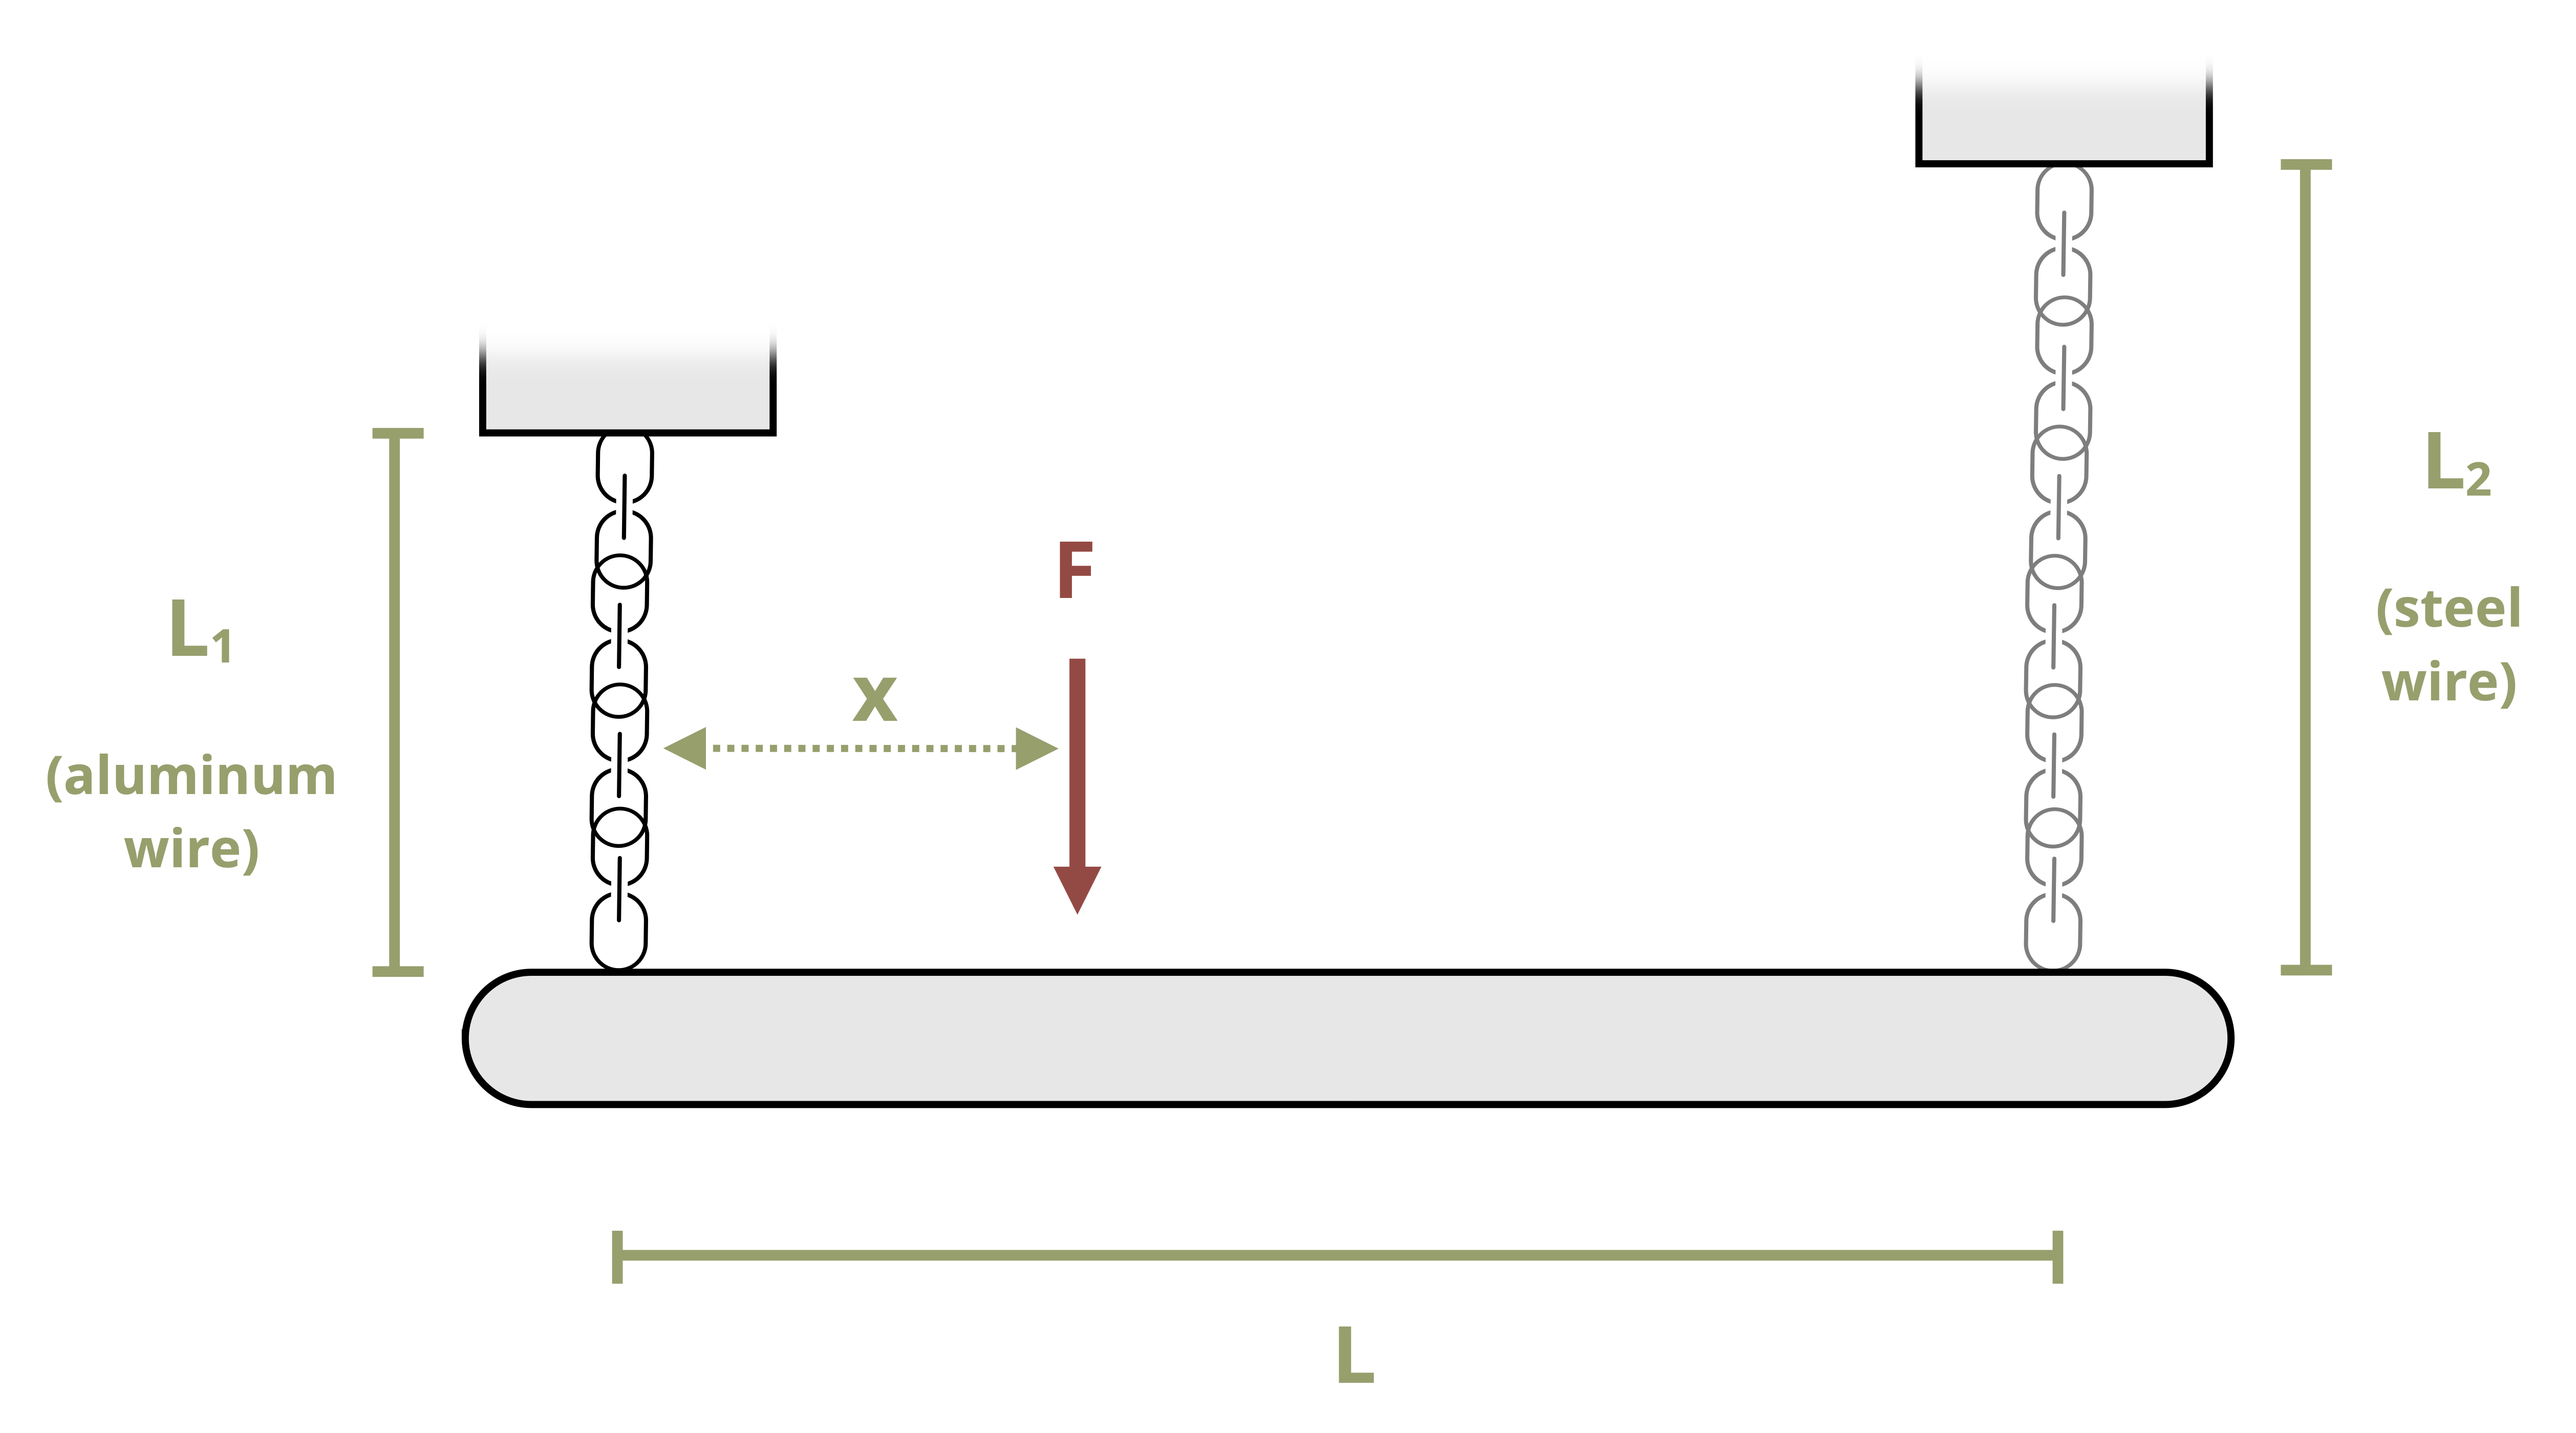
\includegraphics{images/191.png}

}

\caption{Figure 1: A bar is attached to two wires, one steel and one
aluminum.}

\end{figure}%

\begin{Shaded}
\begin{Highlighting}[]
\NormalTok{\#| standalone: true}
\NormalTok{\#| viewerHeight: 600}
\NormalTok{\#| components: [viewer]}

\NormalTok{from shiny import App, render, ui, reactive}
\NormalTok{import random}
\NormalTok{import asyncio}
\NormalTok{import io}
\NormalTok{import math}
\NormalTok{import string}
\NormalTok{from datetime import datetime}
\NormalTok{from pathlib import Path}

\NormalTok{def generate\_random\_letters(length):}
\NormalTok{    \# Generate a random string of letters of specified length}
\NormalTok{    return \textquotesingle{}\textquotesingle{}.join(random.choice(string.ascii\_lowercase) for \_ in range(length))}

\NormalTok{problem\_ID="191"}
\NormalTok{L1=reactive.Value("\_\_")}
\NormalTok{L2=reactive.Value("\_\_")}
\NormalTok{F=reactive.Value("\_\_")}
\NormalTok{A=reactive.Value("\_\_")}
\NormalTok{L=reactive.Value("\_\_")}
\NormalTok{Esteel = 29000}
\NormalTok{Ealuminum = 10000}


\NormalTok{attempts=["Timestamp,Attempt,Answer,Feedback\textbackslash{}n"]}

\NormalTok{app\_ui = ui.page\_fluid(}
\NormalTok{    ui.markdown("**Please enter your ID number from your instructor and click to generate your problem**"),}
\NormalTok{    ui.input\_text("ID","", placeholder="Enter ID Number Here"),}
\NormalTok{    ui.input\_action\_button("generate\_problem", "Generate Problem", class\_="btn{-}primary"),}
\NormalTok{    ui.markdown("**Problem Statement**"),}
\NormalTok{    ui.output\_ui("ui\_problem\_statement"),}
\NormalTok{    ui.input\_text("answer","Your Answer in units of inches", placeholder="Please enter your answer"),}
\NormalTok{    ui.input\_action\_button("submit", "Submit Answer", class\_="btn{-}primary"),}
\NormalTok{    ui.download\_button("download", "Download File to Submit", class\_="btn{-}success"),}
\NormalTok{)}


\NormalTok{def server(input, output, session):}
\NormalTok{    \# Initialize a counter for attempts}
\NormalTok{    attempt\_counter = reactive.Value(0)}

\NormalTok{    @output}
\NormalTok{    @render.ui}
\NormalTok{    def ui\_problem\_statement():}
\NormalTok{        return[ui.markdown(f"A bar is attached to two wires, one steel and one aluminum. If the lengths of the wires L\textless{}sub\textgreater{}1\textless{}/sub\textgreater{} = \{L1()\} in. and L\textless{}sub\textgreater{}2\textless{}/sub\textgreater{} = \{L2()\} in., find the distance x that load F = \{F()\} kips must be placed at so that the bar remains horizontal after the load is applied. Both wires have the same cross{-}section area A = \{A()\} in.\textless{}sup\textgreater{}2\textless{}/sup\textgreater{}. Assume E\textless{}sub\textgreater{}steel\textless{}/sub\textgreater{} = 29,000 ksi, E\textless{}sub\textgreater{}aluminum\textless{}/sub\textgreater{} = 10,000 ksi and that the bar is of length L = \{L()\} in.")]}
    
\NormalTok{    @reactive.Effect}
\NormalTok{    @reactive.event(input.generate\_problem)}
\NormalTok{    def randomize\_vars():}
\NormalTok{        random.seed(input.ID())}
\NormalTok{        L1.set(random.randrange(50, 150, 1)/10)}
\NormalTok{        L2.set(round(L1()*2, 2))}
\NormalTok{        F.set(random.randrange(30, 150, 1)/10)}
\NormalTok{        A.set(random.randrange(2, 25, 1)/100)}
\NormalTok{        L.set(random.randrange(10, 20, 1))}
        
\NormalTok{    @reactive.Effect}
\NormalTok{    @reactive.event(input.submit)}
\NormalTok{    def \_():}
\NormalTok{        attempt\_counter.set(attempt\_counter() + 1)  \# Increment the attempt counter on each submission.}
\NormalTok{        PsPa = (L1()*Esteel*A())/(L2()*Ealuminum*A())}
\NormalTok{        Ps = (F()/(PsPa+1))*PsPa}
\NormalTok{        instr=(Ps*L())/F()}
\NormalTok{        if math.isclose(float(input.answer()), instr, rel\_tol=0.01):}
\NormalTok{            check = "*Correct*"}
\NormalTok{            correct\_indicator = "JL"}
\NormalTok{        else:}
\NormalTok{            check = "*Not Correct.*"}
\NormalTok{            correct\_indicator = "JG"}

\NormalTok{        \# Generate random parts for the encoded attempt.}
\NormalTok{        random\_start = generate\_random\_letters(4)}
\NormalTok{        random\_middle = generate\_random\_letters(4)}
\NormalTok{        random\_end = generate\_random\_letters(4)}
\NormalTok{        encoded\_attempt = f"\{random\_start\}\{problem\_ID\}{-}\{random\_middle\}\{attempt\_counter()\}\{correct\_indicator\}{-}\{random\_end\}\{input.ID()\}"}

\NormalTok{        \# Store the most recent encoded attempt in a reactive value so it persists across submissions}
\NormalTok{        session.encoded\_attempt = reactive.Value(encoded\_attempt)}

\NormalTok{        \# Append the attempt data to the attempts list without the encoded attempt}
\NormalTok{        attempts.append(f"\{datetime.now()\}, \{attempt\_counter()\}, \{input.answer()\}, \{check\}\textbackslash{}n")}

\NormalTok{        \# Show feedback to the user.}
\NormalTok{        feedback = ui.markdown(f"Your answer of \{input.answer()\} is \{check\}.")}
\NormalTok{        m = ui.modal(}
\NormalTok{            feedback,}
\NormalTok{            title="Feedback",}
\NormalTok{            easy\_close=True}
\NormalTok{        )}
\NormalTok{        ui.modal\_show(m)}

\NormalTok{    @session.download(filename=lambda: f"Problem\_Log{-}\{problem\_ID\}{-}\{input.ID()\}.csv")}
\NormalTok{    async def download():}
\NormalTok{        \# Start the CSV with the encoded attempt (without label)}
\NormalTok{        final\_encoded = session.encoded\_attempt() if session.encoded\_attempt is not None else "No attempts"}
\NormalTok{        yield f"\{final\_encoded\}\textbackslash{}n\textbackslash{}n"}
        
\NormalTok{        \# Write the header for the remaining CSV data once}
\NormalTok{        yield "Timestamp,Attempt,Answer,Feedback\textbackslash{}n"}
        
\NormalTok{        \# Write the attempts data, ensure that the header from the attempts list is not written again}
\NormalTok{        for attempt in attempts[1:]:  \# Skip the first element which is the header}
\NormalTok{            await asyncio.sleep(0.25)  \# This delay may not be necessary; adjust as needed}
\NormalTok{            yield attempt}


\NormalTok{\# App installation}
\NormalTok{app = App(app\_ui, server)}
\end{Highlighting}
\end{Shaded}

\chapter*{Problem 5.34}\label{problem-5.34}
\addcontentsline{toc}{chapter}{Problem 5.34}

\markboth{Problem 5.34}{Problem 5.34}

This is a dynamic rendering of the problem with dynamic variables based
on the username entered.

\section*{Problem Image}\label{problem-image-47}
\addcontentsline{toc}{section}{Problem Image}

\markright{Problem Image}

\begin{figure}[H]

{\centering 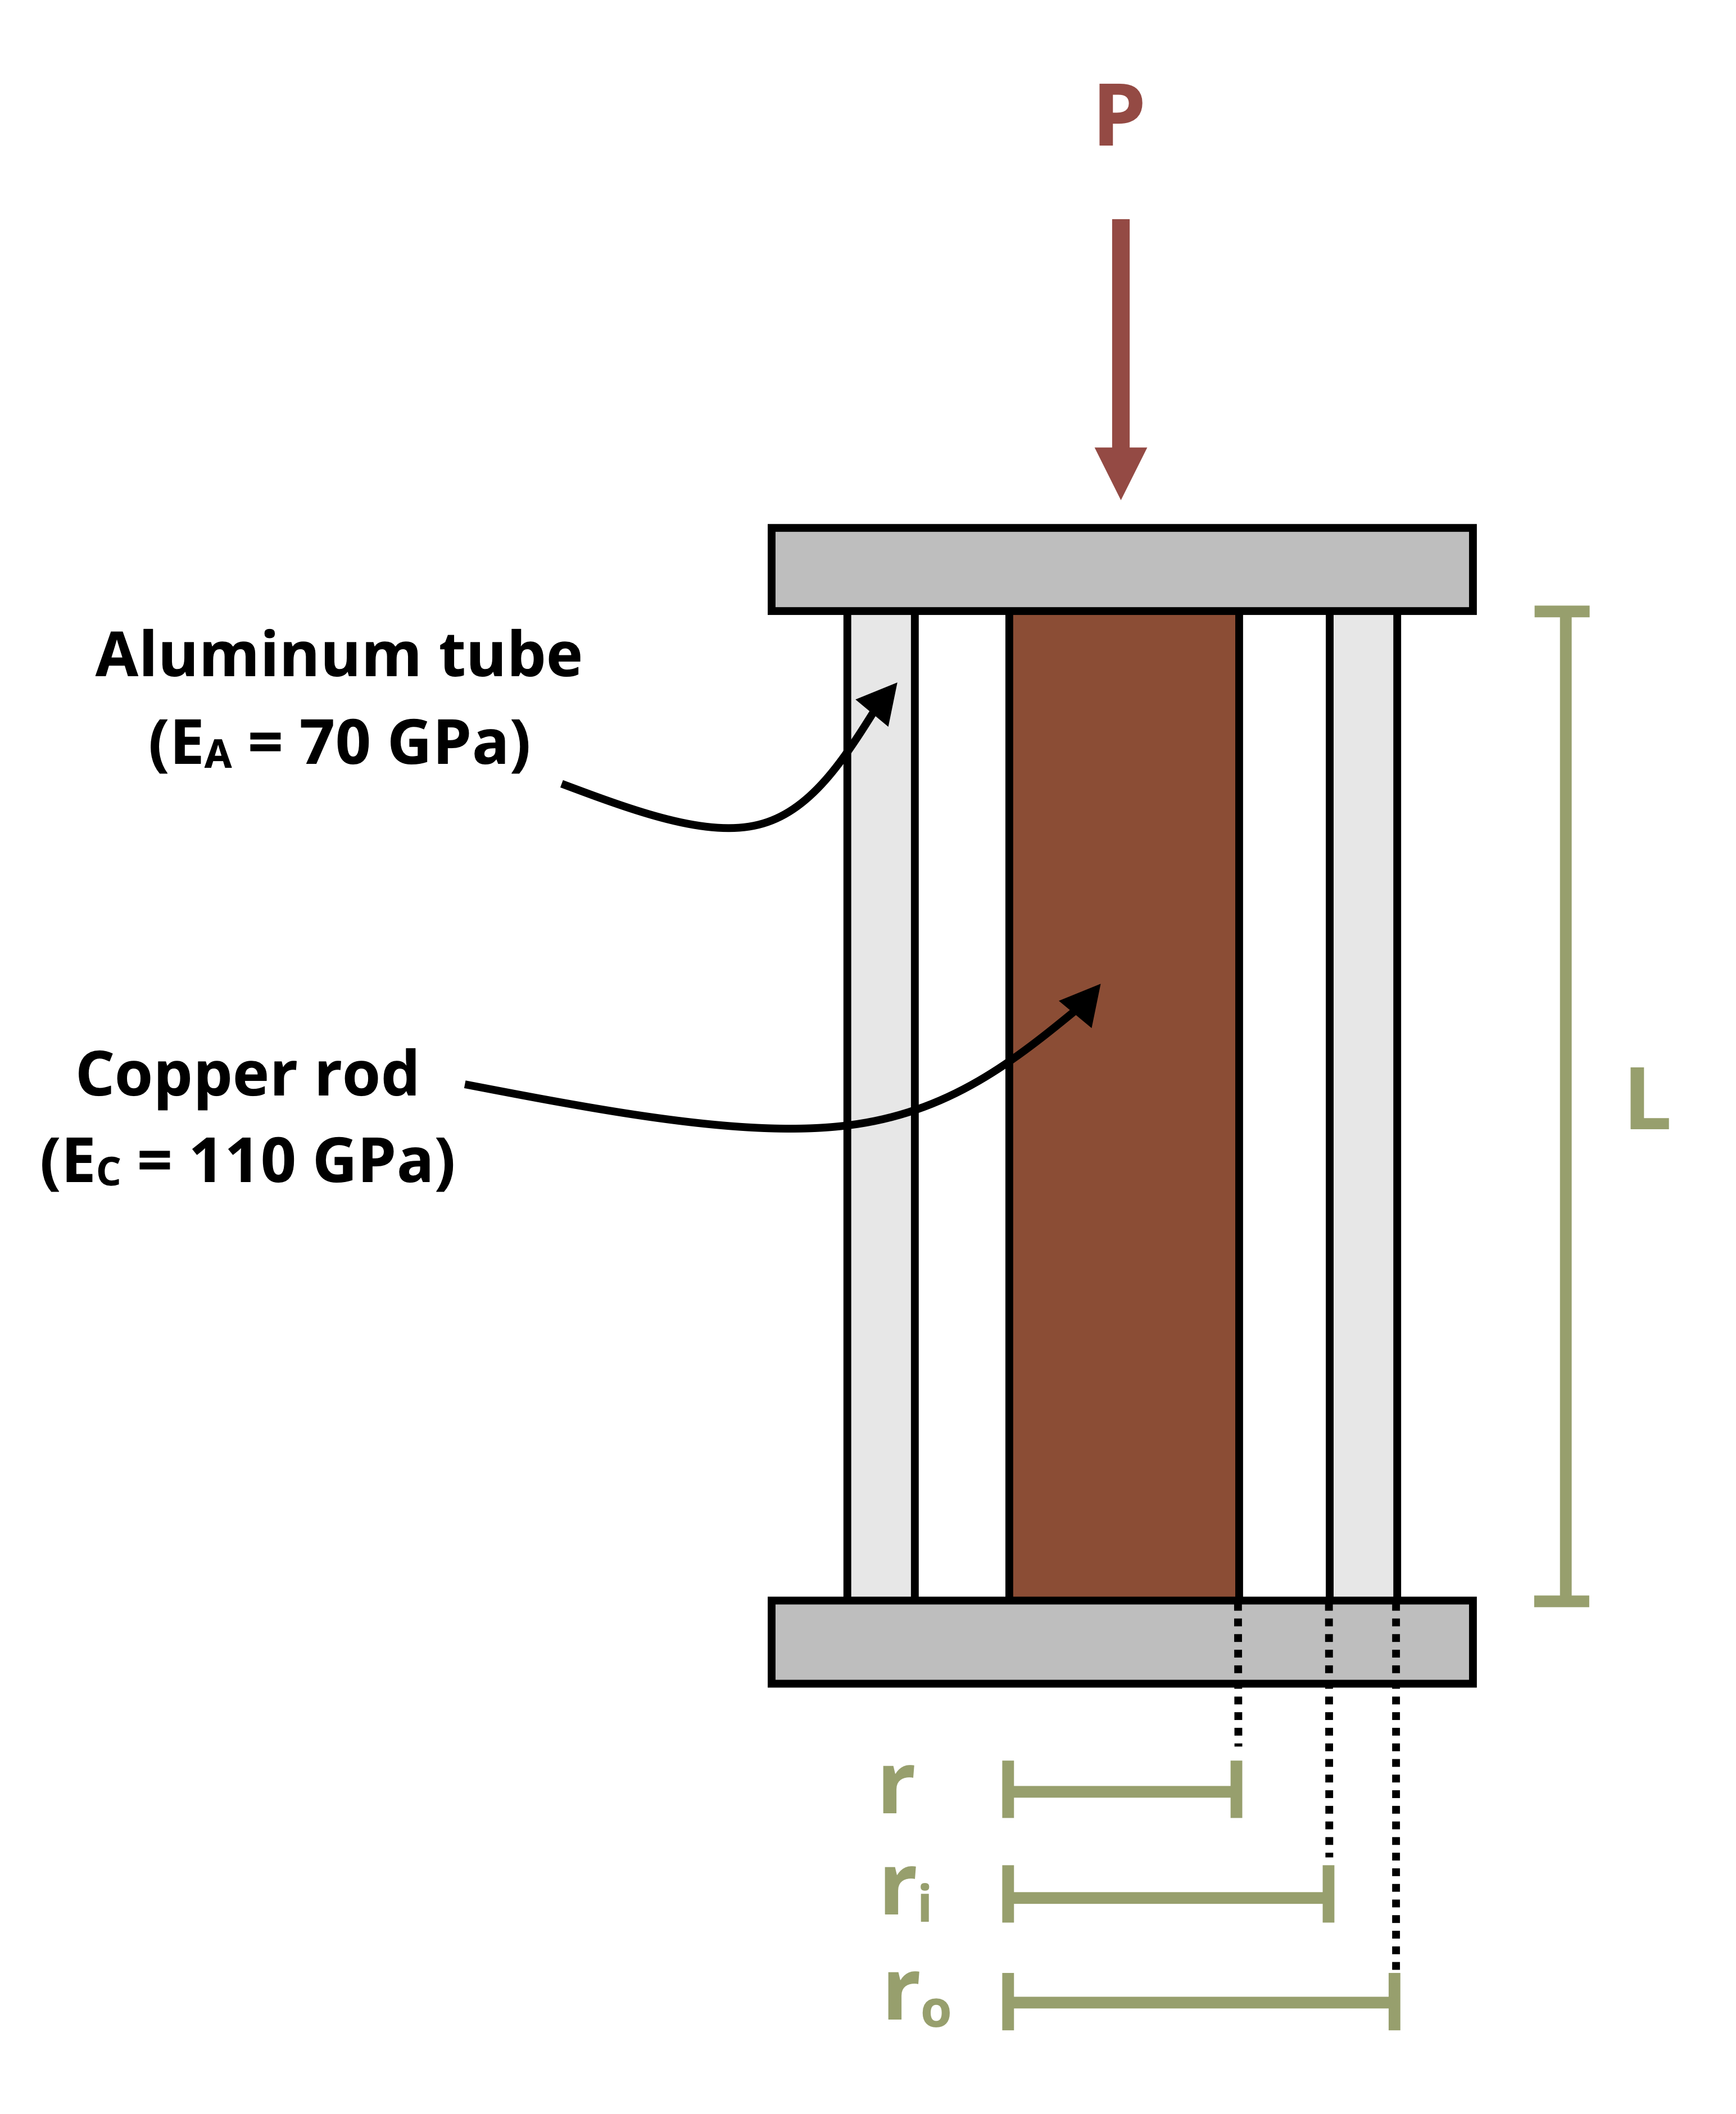
\includegraphics{images/192.png}

}

\caption{Figure 1: A copper circular rod is inserted into an aluminum
tube as shown.}

\end{figure}%

\begin{Shaded}
\begin{Highlighting}[]
\NormalTok{\#| standalone: true}
\NormalTok{\#| viewerHeight: 600}
\NormalTok{\#| components: [viewer]}

\NormalTok{from shiny import App, render, ui, reactive}
\NormalTok{import random}
\NormalTok{import asyncio}
\NormalTok{import io}
\NormalTok{import math}
\NormalTok{import string}
\NormalTok{from datetime import datetime}
\NormalTok{from pathlib import Path}

\NormalTok{def generate\_random\_letters(length):}
\NormalTok{    \# Generate a random string of letters of specified length}
\NormalTok{    return \textquotesingle{}\textquotesingle{}.join(random.choice(string.ascii\_lowercase) for \_ in range(length)) }

\NormalTok{problem\_ID="192"}
\NormalTok{r=reactive.Value("\_\_")}
\NormalTok{ri=reactive.Value("\_\_")}
\NormalTok{ro=reactive.Value("\_\_")}
\NormalTok{L=reactive.Value("\_\_")}
\NormalTok{dL=reactive.Value("\_\_")}
\NormalTok{Ecopper = 110}
\NormalTok{Ealuminum = 70}

\NormalTok{attempts=["Timestamp,Attempt,Answer,Feedback\textbackslash{}n"]}

\NormalTok{app\_ui = ui.page\_fluid(}
\NormalTok{    ui.markdown("**Please enter your ID number from your instructor and click to generate your problem**"),}
\NormalTok{    ui.input\_text("ID","", placeholder="Enter ID Number Here"),}
\NormalTok{    ui.input\_action\_button("generate\_problem", "Generate Problem", class\_="btn{-}primary"),}
\NormalTok{    ui.markdown("**Problem Statement**"),}
\NormalTok{    ui.output\_ui("ui\_problem\_statement"),}
\NormalTok{    ui.input\_text("answer","Your Answer in units of kN", placeholder="Please enter your answer"),}
\NormalTok{    ui.input\_action\_button("submit", "Submit Answer", class\_="btn{-}primary"),}
\NormalTok{    ui.download\_button("download", "Download File to Submit", class\_="btn{-}success"),}
\NormalTok{)}

\NormalTok{def server(input, output, session):}
\NormalTok{    \# Initialize a counter for attempts}
\NormalTok{    attempt\_counter = reactive.Value(0)}

\NormalTok{    @output}
\NormalTok{    @render.ui}
\NormalTok{    def ui\_problem\_statement():}
\NormalTok{        return[ui.markdown(f"A copper circular rod of radius r = \{r()\} cm is inserted into an aluminum tube with inner radius r\textless{}sub\textgreater{}i\textless{}/sub\textgreater{} = \{ri()\} cm and outer radius r\textless{}sub\textgreater{}o\textless{}/sub\textgreater{} = \{ro()\} cm as shown. Load P is applied to the rigid top plate. If length L = \{L()\} cm, what load P will cause the plate to deflect dL = \{dL()\} mm downward? Assume E\textless{}sub\textgreater{}copper\textless{}/sub\textgreater{} = 110 GPa and E\textless{}sub\textgreater{}aluminum\textless{}/sub\textgreater{} = 70 GPa")]}
    
\NormalTok{    @reactive.Effect}
\NormalTok{    @reactive.event(input.generate\_problem)}
\NormalTok{    def randomize\_vars():}
\NormalTok{        random.seed(input.ID())}
\NormalTok{        r.set(random.randrange(20, 60, 1)/10)}
\NormalTok{        ri.set(round(r()*1.25, 2))}
\NormalTok{        ro.set(round(r()*1.5, 2))}
\NormalTok{        L.set(random.randrange(150, 300, 1)/10)}
\NormalTok{        dL.set(random.randrange(10, 50, 1)/100)}
        
\NormalTok{    @reactive.Effect}
\NormalTok{    @reactive.event(input.submit)}
\NormalTok{    def \_():}
\NormalTok{        attempt\_counter.set(attempt\_counter() + 1)  \# Increment the attempt counter on each submission.}
\NormalTok{        instr=(((dL()*Ecopper*r()**2*math.pi)/L()) + ((dL()*Ealuminum*(ro()**2{-}ri()**2)*math.pi)/L()))*10}
\NormalTok{        if math.isclose(float(input.answer()), instr, rel\_tol=0.01):}
\NormalTok{            check = "*Correct*"}
\NormalTok{            correct\_indicator = "JL"}
\NormalTok{        else:}
\NormalTok{            check = "*Not Correct.*"}
\NormalTok{            correct\_indicator = "JG"}

\NormalTok{        \# Generate random parts for the encoded attempt.}
\NormalTok{        random\_start = generate\_random\_letters(4)}
\NormalTok{        random\_middle = generate\_random\_letters(4)}
\NormalTok{        random\_end = generate\_random\_letters(4)}
\NormalTok{        encoded\_attempt = f"\{random\_start\}\{problem\_ID\}{-}\{random\_middle\}\{attempt\_counter()\}\{correct\_indicator\}{-}\{random\_end\}\{input.ID()\}"}

\NormalTok{        \# Store the most recent encoded attempt in a reactive value so it persists across submissions}
\NormalTok{        session.encoded\_attempt = reactive.Value(encoded\_attempt)}

\NormalTok{        \# Append the attempt data to the attempts list without the encoded attempt}
\NormalTok{        attempts.append(f"\{datetime.now()\}, \{attempt\_counter()\}, \{input.answer()\}, \{check\}\textbackslash{}n")}

\NormalTok{        \# Show feedback to the user.}
\NormalTok{        feedback = ui.markdown(f"Your answer of \{input.answer()\} is \{check\}.")}
\NormalTok{        m = ui.modal(}
\NormalTok{            feedback,}
\NormalTok{            title="Feedback",}
\NormalTok{            easy\_close=True}
\NormalTok{        )}
\NormalTok{        ui.modal\_show(m)}

\NormalTok{    @session.download(filename=lambda: f"Problem\_Log{-}\{problem\_ID\}{-}\{input.ID()\}.csv")}
\NormalTok{    async def download():}
\NormalTok{        \# Start the CSV with the encoded attempt (without label)}
\NormalTok{        final\_encoded = session.encoded\_attempt() if session.encoded\_attempt is not None else "No attempts"}
\NormalTok{        yield f"\{final\_encoded\}\textbackslash{}n\textbackslash{}n"}
        
\NormalTok{        \# Write the header for the remaining CSV data once}
\NormalTok{        yield "Timestamp,Attempt,Answer,Feedback\textbackslash{}n"}
        
\NormalTok{        \# Write the attempts data, ensure that the header from the attempts list is not written again}
\NormalTok{        for attempt in attempts[1:]:  \# Skip the first element which is the header}
\NormalTok{            await asyncio.sleep(0.25)  \# This delay may not be necessary; adjust as needed}
\NormalTok{            yield attempt}

\NormalTok{\# App installation}
\NormalTok{app = App(app\_ui, server)}
\end{Highlighting}
\end{Shaded}

\chapter*{Problem 5.35}\label{problem-5.35}
\addcontentsline{toc}{chapter}{Problem 5.35}

\markboth{Problem 5.35}{Problem 5.35}

This is a dynamic rendering of the problem with dynamic variables based
on the username entered.

\section*{Problem Image}\label{problem-image-48}
\addcontentsline{toc}{section}{Problem Image}

\markright{Problem Image}

\begin{figure}[H]

{\centering 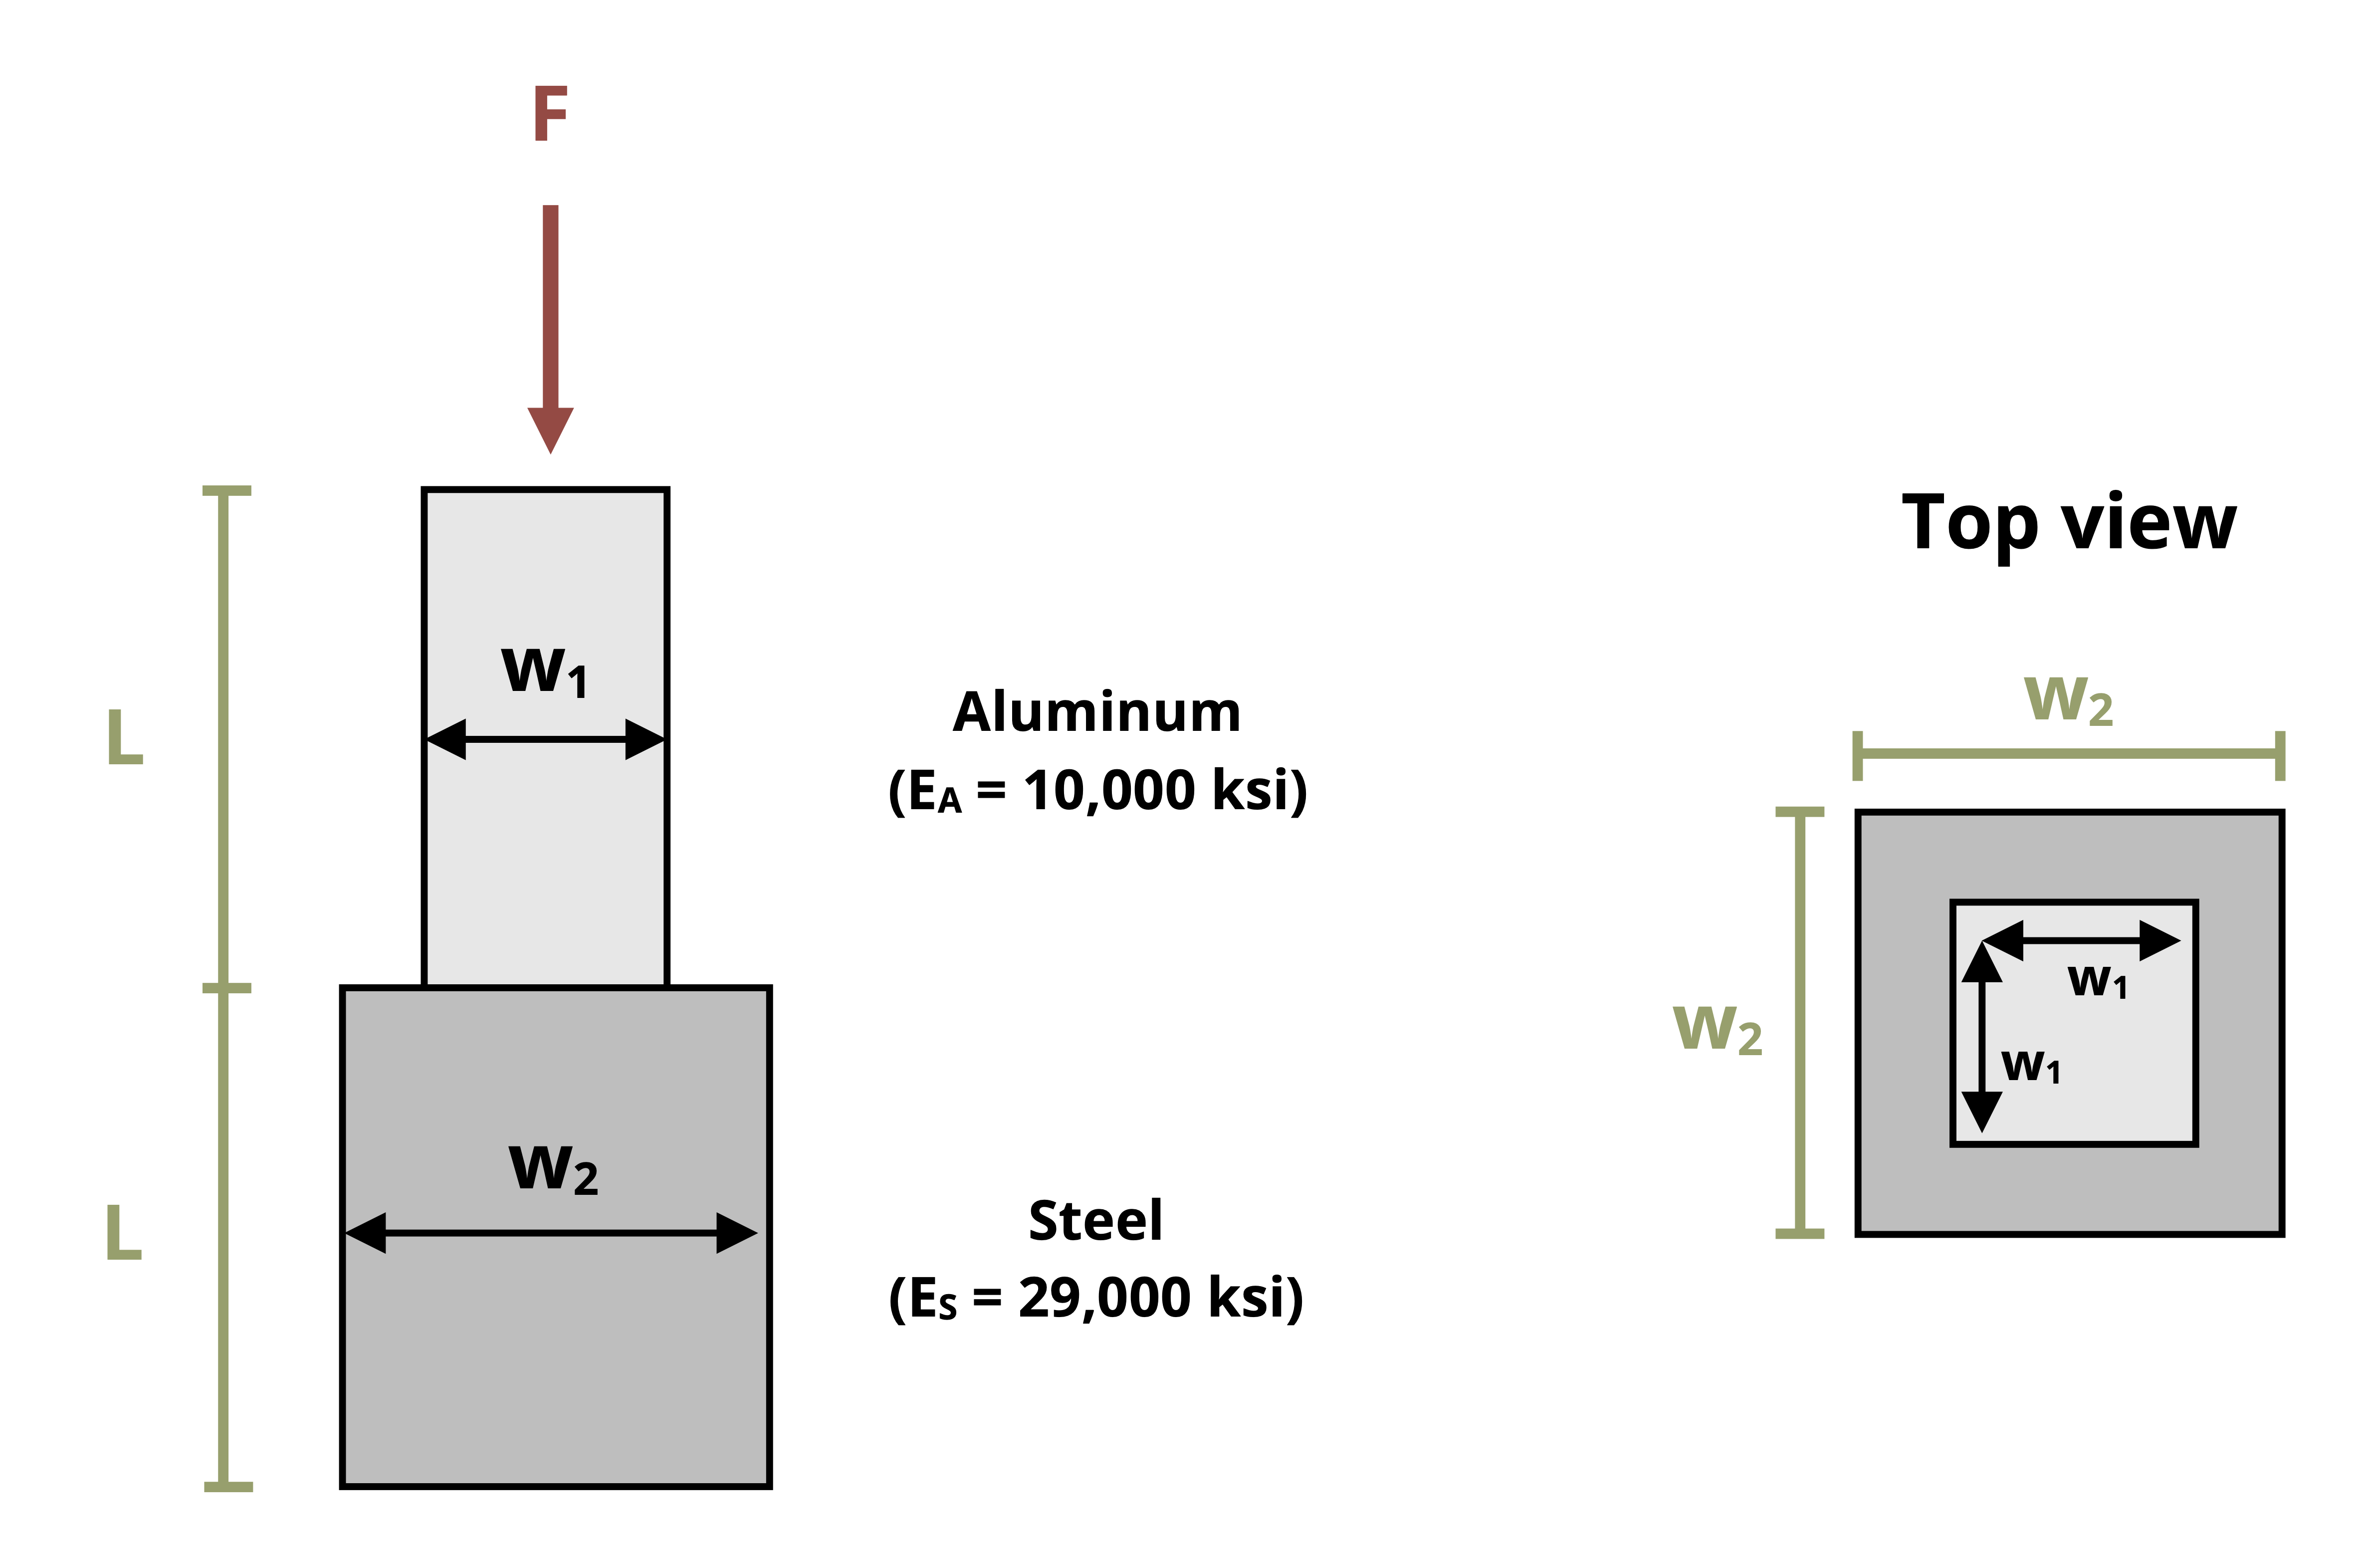
\includegraphics{images/193.png}

}

\caption{Figure 1: Two blocks with square cross sections are stacked and
loaded at the top.}

\end{figure}%

\begin{Shaded}
\begin{Highlighting}[]
\NormalTok{\#| standalone: true}
\NormalTok{\#| viewerHeight: 600}
\NormalTok{\#| components: [viewer]}

\NormalTok{from shiny import App, render, ui, reactive}
\NormalTok{import random}
\NormalTok{import asyncio}
\NormalTok{import io}
\NormalTok{import math}
\NormalTok{import string}
\NormalTok{from datetime import datetime}
\NormalTok{from pathlib import Path}

\NormalTok{def generate\_random\_letters(length):}
\NormalTok{    \# Generate a random string of letters of specified length}
\NormalTok{    return \textquotesingle{}\textquotesingle{}.join(random.choice(string.ascii\_lowercase) for \_ in range(length)) }

\NormalTok{problem\_ID="193"}
\NormalTok{F=reactive.Value("\_\_")}
\NormalTok{w1=reactive.Value("\_\_")}
\NormalTok{w2=reactive.Value("\_\_")}
\NormalTok{L=reactive.Value("\_\_")}
\NormalTok{Esteel = 29000}
\NormalTok{Ealuminum = 10000}



\NormalTok{attempts=["Timestamp,Attempt,Answer,Feedback\textbackslash{}n"]}

\NormalTok{app\_ui = ui.page\_fluid(}
\NormalTok{    ui.markdown("**Please enter your ID number from your instructor and click to generate your problem**"),}
\NormalTok{    ui.input\_text("ID","", placeholder="Enter ID Number Here"),}
\NormalTok{    ui.input\_action\_button("generate\_problem", "Generate Problem", class\_="btn{-}primary"),}
\NormalTok{    ui.markdown("**Problem Statement**"),}
\NormalTok{    ui.output\_ui("ui\_problem\_statement"),}
\NormalTok{    ui.input\_text("answer","Your Answer in units of inches", placeholder="Please enter your answer"),}
\NormalTok{    ui.input\_action\_button("submit", "Submit Answer", class\_="btn{-}primary"),}
\NormalTok{    ui.download\_button("download", "Download File to Submit", class\_="btn{-}success"),}
\NormalTok{)}


\NormalTok{def server(input, output, session):}
\NormalTok{    \# Initialize a counter for attempts}
\NormalTok{    attempt\_counter = reactive.Value(0)}

\NormalTok{    @output}
\NormalTok{    @render.ui}
\NormalTok{    def ui\_problem\_statement():}
\NormalTok{        return[ui.markdown(f"Two blocks with square cross{-}sections are stacked as shown, with the top block inserted into the bottom block and subjected to load F = \{F()\} kips. The top block is aluminum (E = 10,000 ksi) with side length w\textless{}sub\textgreater{}1\textless{}/sub\textgreater{} = \{w1()\} in.  and the bottom block is steel (E = 29,000 ksi) with side length w\textless{}sub\textgreater{}2\textless{}/sub\textgreater{} = \{w2()\} in. If length L = \{L()\} in., what is the total deflection of the top surface? Ignore the weight of the blocks. ")]}
    
\NormalTok{    @reactive.Effect}
\NormalTok{    @reactive.event(input.generate\_problem)}
\NormalTok{    def randomize\_vars():}
\NormalTok{        random.seed(input.ID())}
\NormalTok{        F.set(random.randrange(20, 100, 1)/10)}
\NormalTok{        w1.set(random.randrange(15, 50, 1)/10)}
\NormalTok{        w2.set(round(w1()*1.5))}
\NormalTok{        L.set(random.randrange(50, 200, 1)/10)}
        
\NormalTok{    @reactive.Effect}
\NormalTok{    @reactive.event(input.submit)}
\NormalTok{    def \_():}
\NormalTok{        attempt\_counter.set(attempt\_counter() + 1)  \# Increment the attempt counter on each submission.}
\NormalTok{        instr=F()*L()*((1/((w1()**2)*Ealuminum)) + (1/((w2()**2)*Esteel)))}
\NormalTok{        if math.isclose(float(input.answer()), instr, rel\_tol=0.01):}
\NormalTok{            check = "*Correct*"}
\NormalTok{            correct\_indicator = "JL"}
\NormalTok{        else:}
\NormalTok{            check = "*Not Correct.*"}
\NormalTok{            correct\_indicator = "JG"}

\NormalTok{        \# Generate random parts for the encoded attempt.}
\NormalTok{        random\_start = generate\_random\_letters(4)}
\NormalTok{        random\_middle = generate\_random\_letters(4)}
\NormalTok{        random\_end = generate\_random\_letters(4)}
\NormalTok{        encoded\_attempt = f"\{random\_start\}\{problem\_ID\}{-}\{random\_middle\}\{attempt\_counter()\}\{correct\_indicator\}{-}\{random\_end\}\{input.ID()\}"}

\NormalTok{        \# Store the most recent encoded attempt in a reactive value so it persists across submissions}
\NormalTok{        session.encoded\_attempt = reactive.Value(encoded\_attempt)}

\NormalTok{        \# Append the attempt data to the attempts list without the encoded attempt}
\NormalTok{        attempts.append(f"\{datetime.now()\}, \{attempt\_counter()\}, \{input.answer()\}, \{check\}\textbackslash{}n")}

\NormalTok{        \# Show feedback to the user.}
\NormalTok{        feedback = ui.markdown(f"Your answer of \{input.answer()\} is \{check\}.")}
\NormalTok{        m = ui.modal(}
\NormalTok{            feedback,}
\NormalTok{            title="Feedback",}
\NormalTok{            easy\_close=True}
\NormalTok{        )}
\NormalTok{        ui.modal\_show(m)}

\NormalTok{    @session.download(filename=lambda: f"Problem\_Log{-}\{problem\_ID\}{-}\{input.ID()\}.csv")}
\NormalTok{    async def download():}
\NormalTok{        \# Start the CSV with the encoded attempt (without label)}
\NormalTok{        final\_encoded = session.encoded\_attempt() if session.encoded\_attempt is not None else "No attempts"}
\NormalTok{        yield f"\{final\_encoded\}\textbackslash{}n\textbackslash{}n"}
        
\NormalTok{        \# Write the header for the remaining CSV data once}
\NormalTok{        yield "Timestamp,Attempt,Answer,Feedback\textbackslash{}n"}
        
\NormalTok{        \# Write the attempts data, ensure that the header from the attempts list is not written again}
\NormalTok{        for attempt in attempts[1:]:  \# Skip the first element which is the header}
\NormalTok{            await asyncio.sleep(0.25)  \# This delay may not be necessary; adjust as needed}
\NormalTok{            yield attempt}


\NormalTok{\# App installation}
\NormalTok{app = App(app\_ui, server)}
\end{Highlighting}
\end{Shaded}

\chapter*{Problem 5.36}\label{problem-5.36}
\addcontentsline{toc}{chapter}{Problem 5.36}

\markboth{Problem 5.36}{Problem 5.36}

This is a dynamic rendering of the problem with dynamic variables based
on the username entered.

\section*{Problem Image}\label{problem-image-49}
\addcontentsline{toc}{section}{Problem Image}

\markright{Problem Image}

\includegraphics{images/246.png}\{fig-alt='' Two square members are
placed between two fixed walls. The wood piece is on the left and the
plastic piece is on the right. Point B is at the intersection of the
wood and plastic members. The members are each length L. ``\}

\begin{Shaded}
\begin{Highlighting}[]
\NormalTok{\#| standalone: true}
\NormalTok{\#| viewerHeight: 600}
\NormalTok{\#| components: [viewer]}

\NormalTok{from shiny import App, render, ui, reactive}
\NormalTok{import random}
\NormalTok{import asyncio}
\NormalTok{import io}
\NormalTok{import math}
\NormalTok{import string}
\NormalTok{from datetime import datetime}
\NormalTok{from pathlib import Path}

\NormalTok{def generate\_random\_letters(length):}
\NormalTok{    \# Generate a random string of letters of specified length}
\NormalTok{    return \textquotesingle{}\textquotesingle{}.join(random.choice(string.ascii\_lowercase) for \_ in range(length)) }

\NormalTok{problem\_ID="246"}
\NormalTok{d=reactive.Value("\_\_")}
\NormalTok{L=reactive.Value("\_\_")}
\NormalTok{Eplastic=reactive.Value("\_\_")}
\NormalTok{Ewood=1750}

\NormalTok{attempts=["Timestamp,Attempt,Answer,Feedback\textbackslash{}n"]}

\NormalTok{app\_ui = ui.page\_fluid(}
\NormalTok{    ui.markdown("**Please enter your ID number from your instructor and click to generate your problem**"),}
\NormalTok{    ui.input\_text("ID","", placeholder="Enter ID Number Here"),}
\NormalTok{    ui.input\_action\_button("generate\_problem", "Generate Problem", class\_="btn{-}primary"),}
\NormalTok{    ui.markdown("**Problem Statement**"),}
\NormalTok{    ui.output\_ui("ui\_problem\_statement"),}
\NormalTok{    ui.input\_text("answer","Your Answer in units of lb", placeholder="Please enter your answer"),}
\NormalTok{    ui.input\_action\_button("submit", "Submit Answer", class\_="btn{-}primary"),}
\NormalTok{    ui.download\_button("download", "Download File to Submit", class\_="btn{-}success"),}
\NormalTok{)}


\NormalTok{def server(input, output, session):}
\NormalTok{    \# Initialize a counter for attempts}
\NormalTok{    attempt\_counter = reactive.Value(0)}

\NormalTok{    @output}
\NormalTok{    @render.ui}
\NormalTok{    def ui\_problem\_statement():}
\NormalTok{        return[ui.markdown(f"Two square members are attached to two fixed walls as shown. Force F is applied at point B and point B is displaced d =  \{d()\} in. to the right. If L = \{L()\} in., E\textless{}sub\textgreater{}wood\textless{}/sub\textgreater{} = 1,750 ksi, and E\textless{}sub\textgreater{}plastic\textless{}/sub\textgreater{} = \{Eplastic()\} ksi, determine the applied force F. ")]}
    
\NormalTok{    @reactive.Effect}
\NormalTok{    @reactive.event(input.generate\_problem)}
\NormalTok{    def randomize\_vars():}
\NormalTok{        random.seed(input.ID())}
\NormalTok{        d.set(random.randrange(2, 8, 1)/1000)}
\NormalTok{        L.set(random.randrange(4, 15, 1))}
\NormalTok{        Eplastic.set(random.randrange(350, 900, 10))}
       
\NormalTok{    @reactive.Effect}
\NormalTok{    @reactive.event(input.submit)}
\NormalTok{    def \_():}
\NormalTok{        attempt\_counter.set(attempt\_counter() + 1)  \# Increment the attempt counter on each submission.}
\NormalTok{        instr= (d()*1*Ewood*1000)/L() {-} ({-}d()*4*Eplastic()*1000)/L() }
\NormalTok{        if math.isclose(float(input.answer()), instr, rel\_tol=0.01):}
\NormalTok{            check = "*Correct*"}
\NormalTok{            correct\_indicator = "JL"}
\NormalTok{        else:}
\NormalTok{            check = "*Not Correct.*"}
\NormalTok{            correct\_indicator = "JG"}

\NormalTok{        \# Generate random parts for the encoded attempt.}
\NormalTok{        random\_start = generate\_random\_letters(4)}
\NormalTok{        random\_middle = generate\_random\_letters(4)}
\NormalTok{        random\_end = generate\_random\_letters(4)}
\NormalTok{        encoded\_attempt = f"\{random\_start\}\{problem\_ID\}{-}\{random\_middle\}\{attempt\_counter()\}\{correct\_indicator\}{-}\{random\_end\}\{input.ID()\}"}

\NormalTok{        \# Store the most recent encoded attempt in a reactive value so it persists across submissions}
\NormalTok{        session.encoded\_attempt = reactive.Value(encoded\_attempt)}

\NormalTok{        \# Append the attempt data to the attempts list without the encoded attempt}
\NormalTok{        attempts.append(f"\{datetime.now()\}, \{attempt\_counter()\}, \{input.answer()\}, \{check\}\textbackslash{}n")}

\NormalTok{        \# Show feedback to the user.}
\NormalTok{        feedback = ui.markdown(f"Your answer of \{input.answer()\} is \{check\}.")}
\NormalTok{        m = ui.modal(}
\NormalTok{            feedback,}
\NormalTok{            title="Feedback",}
\NormalTok{            easy\_close=True}
\NormalTok{        )}
\NormalTok{        ui.modal\_show(m)}

\NormalTok{    @session.download(filename=lambda: f"Problem\_Log{-}\{problem\_ID\}{-}\{input.ID()\}.csv")}
\NormalTok{    async def download():}
\NormalTok{        \# Start the CSV with the encoded attempt (without label)}
\NormalTok{        final\_encoded = session.encoded\_attempt() if session.encoded\_attempt is not None else "No attempts"}
\NormalTok{        yield f"\{final\_encoded\}\textbackslash{}n\textbackslash{}n"}
        
\NormalTok{        \# Write the header for the remaining CSV data once}
\NormalTok{        yield "Timestamp,Attempt,Answer,Feedback\textbackslash{}n"}
        
\NormalTok{        \# Write the attempts data, ensure that the header from the attempts list is not written again}
\NormalTok{        for attempt in attempts[1:]:  \# Skip the first element which is the header}
\NormalTok{            await asyncio.sleep(0.25)  \# This delay may not be necessary; adjust as needed}
\NormalTok{            yield attempt}

\NormalTok{\# App installation}
\NormalTok{app = App(app\_ui, server)}
\end{Highlighting}
\end{Shaded}

\chapter*{Problem 5.37}\label{problem-5.37}
\addcontentsline{toc}{chapter}{Problem 5.37}

\markboth{Problem 5.37}{Problem 5.37}

This is a dynamic rendering of the problem with dynamic variables based
on the username entered.

\section*{Problem Image}\label{problem-image-50}
\addcontentsline{toc}{section}{Problem Image}

\markright{Problem Image}

\includegraphics{images/247.png}\{fig-alt='' Two aluminum circular rods
are placed between two fixed walls. Member 1 is on the left and member 2
is on the right. Member 2 has diameter d{[}1{]} and length L{[}1{]}.
Member 2 has diameter d{[}2{]} and length L{[}2{]} ``\}

\begin{Shaded}
\begin{Highlighting}[]
\NormalTok{\#| standalone: true}
\NormalTok{\#| viewerHeight: 600}
\NormalTok{\#| components: [viewer]}

\NormalTok{from shiny import App, render, ui, reactive}
\NormalTok{import random}
\NormalTok{import asyncio}
\NormalTok{import io}
\NormalTok{import math}
\NormalTok{import string}
\NormalTok{from datetime import datetime}
\NormalTok{from pathlib import Path}

\NormalTok{def generate\_random\_letters(length):}
\NormalTok{    \# Generate a random string of letters of specified length}
\NormalTok{    return \textquotesingle{}\textquotesingle{}.join(random.choice(string.ascii\_lowercase) for \_ in range(length)) }

\NormalTok{problem\_ID="247"}
\NormalTok{F=reactive.Value("\_\_")}
\NormalTok{d1=reactive.Value("\_\_")}
\NormalTok{d2=reactive.Value("\_\_")}
\NormalTok{L1=reactive.Value("\_\_")}
\NormalTok{L2=reactive.Value("\_\_")}
\NormalTok{Ewood=70}

\NormalTok{attempts=["Timestamp,Attempt,Answer,Feedback\textbackslash{}n"]}

\NormalTok{app\_ui = ui.page\_fluid(}
\NormalTok{    ui.markdown("**Please enter your ID number from your instructor and click to generate your problem**"),}
\NormalTok{    ui.input\_text("ID","", placeholder="Enter ID Number Here"),}
\NormalTok{    ui.input\_action\_button("generate\_problem", "Generate Problem", class\_="btn{-}primary"),}
\NormalTok{    ui.markdown("**Problem Statement**"),}
\NormalTok{    ui.output\_ui("ui\_problem\_statement"),}
\NormalTok{    ui.input\_text("answer","Your Answer in units of MPa", placeholder="Please enter your answer"),}
\NormalTok{    ui.input\_action\_button("submit", "Submit Answer", class\_="btn{-}primary"),}
\NormalTok{    ui.download\_button("download", "Download File to Submit", class\_="btn{-}success"),}
\NormalTok{)}


\NormalTok{def server(input, output, session):}
\NormalTok{    \# Initialize a counter for attempts}
\NormalTok{    attempt\_counter = reactive.Value(0)}

\NormalTok{    @output}
\NormalTok{    @render.ui}
\NormalTok{    def ui\_problem\_statement():}
\NormalTok{        return[ui.markdown(f"Two aluminum circular rods are attached to two fixed walls as shown. Assume E = 70 MPa for both cylinders, F = \{F()\} kN, d\textless{}sub\textgreater{}1\textless{}/sub\textgreater{} = \{d1()\} mm, d\textless{}sub\textgreater{}2\textless{}/sub\textgreater{}  = \{d2()\} mm, L\textless{}sub\textgreater{}1\textless{}/sub\textgreater{}  = \{L1()\} mm, and L\textless{}sub\textgreater{}2\textless{}/sub\textgreater{}  = \{L2()\} mm. Determine the normal stress in member 1.")]}
    
\NormalTok{    @reactive.Effect}
\NormalTok{    @reactive.event(input.generate\_problem)}
\NormalTok{    def randomize\_vars():}
\NormalTok{        random.seed(input.ID())}
\NormalTok{        F.set(random.randrange(20, 100, 1))}
\NormalTok{        d1.set(random.randrange(15, 50, 1))}
\NormalTok{        d2.set(round(d1()*1.5))}
\NormalTok{        L1.set(random.randrange(200, 800, 10))}
\NormalTok{        L2.set(round(L1()*(2/3)))}
       
        
\NormalTok{    @reactive.Effect}
\NormalTok{    @reactive.event(input.submit)}
\NormalTok{    def \_():}
\NormalTok{        attempt\_counter.set(attempt\_counter() + 1)  \# Increment the attempt counter on each submission.}
\NormalTok{        LHS = (L1()/1000)/(math.pi*(d1()/2000)**2) + (L2()/1000)/(math.pi*(d2()/2000)**2)}
\NormalTok{        RHS = (F()*L2())/(math.pi*(d2()/2)**2)}
\NormalTok{        instr= (RHS/LHS)/(math.pi*(d1()/2000)**2)}
\NormalTok{        if math.isclose(float(input.answer()), instr, rel\_tol=0.01):}
\NormalTok{            check = "*Correct*"}
\NormalTok{            correct\_indicator = "JL"}
\NormalTok{        else:}
\NormalTok{            check = "*Not Correct.*"}
\NormalTok{            correct\_indicator = "JG"}

\NormalTok{        \# Generate random parts for the encoded attempt.}
\NormalTok{        random\_start = generate\_random\_letters(4)}
\NormalTok{        random\_middle = generate\_random\_letters(4)}
\NormalTok{        random\_end = generate\_random\_letters(4)}
\NormalTok{        encoded\_attempt = f"\{random\_start\}\{problem\_ID\}{-}\{random\_middle\}\{attempt\_counter()\}\{correct\_indicator\}{-}\{random\_end\}\{input.ID()\}"}

\NormalTok{        \# Store the most recent encoded attempt in a reactive value so it persists across submissions}
\NormalTok{        session.encoded\_attempt = reactive.Value(encoded\_attempt)}

\NormalTok{        \# Append the attempt data to the attempts list without the encoded attempt}
\NormalTok{        attempts.append(f"\{datetime.now()\}, \{attempt\_counter()\}, \{input.answer()\}, \{check\}\textbackslash{}n")}

\NormalTok{        \# Show feedback to the user.}
\NormalTok{        feedback = ui.markdown(f"Your answer of \{input.answer()\} is \{check\}.")}
\NormalTok{        m = ui.modal(}
\NormalTok{            feedback,}
\NormalTok{            title="Feedback",}
\NormalTok{            easy\_close=True}
\NormalTok{        )}
\NormalTok{        ui.modal\_show(m)}

\NormalTok{    @session.download(filename=lambda: f"Problem\_Log{-}\{problem\_ID\}{-}\{input.ID()\}.csv")}
\NormalTok{    async def download():}
\NormalTok{        \# Start the CSV with the encoded attempt (without label)}
\NormalTok{        final\_encoded = session.encoded\_attempt() if session.encoded\_attempt is not None else "No attempts"}
\NormalTok{        yield f"\{final\_encoded\}\textbackslash{}n\textbackslash{}n"}
        
\NormalTok{        \# Write the header for the remaining CSV data once}
\NormalTok{        yield "Timestamp,Attempt,Answer,Feedback\textbackslash{}n"}
        
\NormalTok{        \# Write the attempts data, ensure that the header from the attempts list is not written again}
\NormalTok{        for attempt in attempts[1:]:  \# Skip the first element which is the header}
\NormalTok{            await asyncio.sleep(0.25)  \# This delay may not be necessary; adjust as needed}
\NormalTok{            yield attempt}


\NormalTok{\# App installation}
\NormalTok{app = App(app\_ui, server)}
\end{Highlighting}
\end{Shaded}

\chapter*{Problem 5.38}\label{problem-5.38}
\addcontentsline{toc}{chapter}{Problem 5.38}

\markboth{Problem 5.38}{Problem 5.38}

This is a dynamic rendering of the problem with dynamic variables based
on the username entered.

\section*{Problem Image}\label{problem-image-51}
\addcontentsline{toc}{section}{Problem Image}

\markright{Problem Image}

\includegraphics{images/248.png}\{fig-alt='' A pressure load is applied
to a short column made of wood and concrete. Concerete is the center of
the column and it is surrounded by wood. The side of the column is 3 *
b, with the width of the wood, concrete, and wood each being b. The
other side of the column is h{[}1{]} + h{[}2{]} + h{[}1{]}, with the
length of the wood being h{[}1{]} and the length of the concrete being
h{[}2{]}.''\}

\begin{Shaded}
\begin{Highlighting}[]
\NormalTok{\#| standalone: true}
\NormalTok{\#| viewerHeight: 600}
\NormalTok{\#| components: [viewer]}

\NormalTok{from shiny import App, render, ui, reactive}
\NormalTok{import random}
\NormalTok{import asyncio}
\NormalTok{import io}
\NormalTok{import math}
\NormalTok{import string}
\NormalTok{from datetime import datetime}
\NormalTok{from pathlib import Path}

\NormalTok{def generate\_random\_letters(length):}
\NormalTok{    \# Generate a random string of letters of specified length}
\NormalTok{    return \textquotesingle{}\textquotesingle{}.join(random.choice(string.ascii\_lowercase) for \_ in range(length)) }

\NormalTok{problem\_ID="248"}
\NormalTok{w=reactive.Value("\_\_")}
\NormalTok{b=reactive.Value("\_\_")}
\NormalTok{h1=reactive.Value("\_\_")}
\NormalTok{h2=reactive.Value("\_\_")}
\NormalTok{Econcrete=25}
\NormalTok{Ewood=12}

\NormalTok{attempts=["Timestamp,Attempt,Answer,Feedback\textbackslash{}n"]}

\NormalTok{app\_ui = ui.page\_fluid(}
\NormalTok{    ui.markdown("**Please enter your ID number from your instructor and click to generate your problem**"),}
\NormalTok{    ui.input\_text("ID","", placeholder="Enter ID Number Here"),}
\NormalTok{    ui.input\_action\_button("generate\_problem", "Generate Problem", class\_="btn{-}primary"),}
\NormalTok{    ui.markdown("**Problem Statement**"),}
\NormalTok{    ui.output\_ui("ui\_problem\_statement"),}
\NormalTok{    ui.input\_text("answer","Your Answer in units of kN", placeholder="Please enter your answer"),}
\NormalTok{    ui.input\_action\_button("submit", "Submit Answer", class\_="btn{-}primary"),}
\NormalTok{    ui.download\_button("download", "Download File to Submit", class\_="btn{-}success"),}
\NormalTok{)}


\NormalTok{def server(input, output, session):}
\NormalTok{    \# Initialize a counter for attempts}
\NormalTok{    attempt\_counter = reactive.Value(0)}

\NormalTok{    @output}
\NormalTok{    @render.ui}
\NormalTok{    def ui\_problem\_statement():}
\NormalTok{        return[ui.markdown(f"A distributed load w = \{w()\} N/cm\textless{}sup\textgreater{}2\textless{}/sup\textgreater{} is applied to a short column made from wood and concrete. Assume E\textless{}sub\textgreater{}concrete \textless{}/sub\textgreater{}= 25 GPa, E\textless{}sub\textgreater{}wood\textless{}/sub\textgreater{} = 12 GPa, b = \{b()\} cm, h\textless{}sub\textgreater{}1\textless{}/sub\textgreater{} = \{h1()\} cm, and h\textless{}sub\textgreater{}2\textless{}/sub\textgreater{} = \{h2()\} cm. What load is carried by the concrete center?")]}
    
\NormalTok{    @reactive.Effect}
\NormalTok{    @reactive.event(input.generate\_problem)}
\NormalTok{    def randomize\_vars():}
\NormalTok{        random.seed(input.ID())}
\NormalTok{        w.set(random.randrange(50, 750, 10))}
\NormalTok{        b.set(random.randrange(20, 100, 1)/10)}
\NormalTok{        h1.set(b()*1)}
\NormalTok{        h2.set(b()*2)}
        
\NormalTok{    @reactive.Effect}
\NormalTok{    @reactive.event(input.submit)}
\NormalTok{    def \_():}
\NormalTok{        attempt\_counter.set(attempt\_counter() + 1)  \# Increment the attempt counter on each submission.}
\NormalTok{        instr= (2.0833*h2()*w()*(2*h1()+h2())*3*b())/(6*h1()+4.0833*h2())/1000}
\NormalTok{        if math.isclose(float(input.answer()), instr, rel\_tol=0.01):}
\NormalTok{            check = "*Correct*"}
\NormalTok{            correct\_indicator = "JL"}
\NormalTok{        else:}
\NormalTok{            check = "*Not Correct.*"}
\NormalTok{            correct\_indicator = "JG"}

\NormalTok{        \# Generate random parts for the encoded attempt.}
\NormalTok{        random\_start = generate\_random\_letters(4)}
\NormalTok{        random\_middle = generate\_random\_letters(4)}
\NormalTok{        random\_end = generate\_random\_letters(4)}
\NormalTok{        encoded\_attempt = f"\{random\_start\}\{problem\_ID\}{-}\{random\_middle\}\{attempt\_counter()\}\{correct\_indicator\}{-}\{random\_end\}\{input.ID()\}"}

\NormalTok{        \# Store the most recent encoded attempt in a reactive value so it persists across submissions}
\NormalTok{        session.encoded\_attempt = reactive.Value(encoded\_attempt)}

\NormalTok{        \# Append the attempt data to the attempts list without the encoded attempt}
\NormalTok{        attempts.append(f"\{datetime.now()\}, \{attempt\_counter()\}, \{input.answer()\}, \{check\}\textbackslash{}n")}

\NormalTok{        \# Show feedback to the user.}
\NormalTok{        feedback = ui.markdown(f"Your answer of \{input.answer()\} is \{check\}.")}
\NormalTok{        m = ui.modal(}
\NormalTok{            feedback,}
\NormalTok{            title="Feedback",}
\NormalTok{            easy\_close=True}
\NormalTok{        )}
\NormalTok{        ui.modal\_show(m)}

\NormalTok{    @session.download(filename=lambda: f"Problem\_Log{-}\{problem\_ID\}{-}\{input.ID()\}.csv")}
\NormalTok{    async def download():}
\NormalTok{        \# Start the CSV with the encoded attempt (without label)}
\NormalTok{        final\_encoded = session.encoded\_attempt() if session.encoded\_attempt is not None else "No attempts"}
\NormalTok{        yield f"\{final\_encoded\}\textbackslash{}n\textbackslash{}n"}
        
\NormalTok{        \# Write the header for the remaining CSV data once}
\NormalTok{        yield "Timestamp,Attempt,Answer,Feedback\textbackslash{}n"}
        
\NormalTok{        \# Write the attempts data, ensure that the header from the attempts list is not written again}
\NormalTok{        for attempt in attempts[1:]:  \# Skip the first element which is the header}
\NormalTok{            await asyncio.sleep(0.25)  \# This delay may not be necessary; adjust as needed}
\NormalTok{            yield attempt}


\NormalTok{\# App installation}
\NormalTok{app = App(app\_ui, server)}
\end{Highlighting}
\end{Shaded}

\chapter*{Problem 5.39}\label{problem-5.39}
\addcontentsline{toc}{chapter}{Problem 5.39}

\markboth{Problem 5.39}{Problem 5.39}

This is a dynamic rendering of the problem with dynamic variables based
on the username entered.

\section*{Problem Image}\label{problem-image-52}
\addcontentsline{toc}{section}{Problem Image}

\markright{Problem Image}

\includegraphics{images/250.png}\{fig-alt='' A concrete post with 6
steel rebar rods embedded in the concrete supports a load, F. The post
has diamete d{[}c{]} and the rebar rods have diamete d{[}s{]}. ``\}

\begin{Shaded}
\begin{Highlighting}[]
\NormalTok{\#| standalone: true}
\NormalTok{\#| viewerHeight: 600}
\NormalTok{\#| components: [viewer]}

\NormalTok{from shiny import App, render, ui, reactive}
\NormalTok{import random}
\NormalTok{import asyncio}
\NormalTok{import io}
\NormalTok{import math}
\NormalTok{import string}
\NormalTok{from datetime import datetime}
\NormalTok{from pathlib import Path}

\NormalTok{def generate\_random\_letters(length):}
\NormalTok{    \# Generate a random string of letters of specified length}
\NormalTok{    return \textquotesingle{}\textquotesingle{}.join(random.choice(string.ascii\_lowercase) for \_ in range(length)) }

\NormalTok{problem\_ID="250"}
\NormalTok{F=reactive.Value("\_\_")}
\NormalTok{L=reactive.Value("\_\_")}
\NormalTok{dc=reactive.Value("\_\_")}
\NormalTok{ds=reactive.Value("\_\_")}
\NormalTok{Econcrete=25}
\NormalTok{Esteel=200}

\NormalTok{attempts=["Timestamp,Attempt,Answer,Feedback\textbackslash{}n"]}

\NormalTok{app\_ui = ui.page\_fluid(}
\NormalTok{    ui.markdown("**Please enter your ID number from your instructor and click to generate your problem**"),}
\NormalTok{    ui.input\_text("ID","", placeholder="Enter ID Number Here"),}
\NormalTok{    ui.input\_action\_button("generate\_problem", "Generate Problem", class\_="btn{-}primary"),}
\NormalTok{    ui.markdown("**Problem Statement**"),}
\NormalTok{    ui.output\_ui("ui\_problem\_statement"),}
\NormalTok{    ui.input\_text("answer","Your Answer in units of MPa", placeholder="Please enter your answer"),}
\NormalTok{    ui.input\_action\_button("submit", "Submit Answer", class\_="btn{-}primary"),}
\NormalTok{    ui.download\_button("download", "Download File to Submit", class\_="btn{-}success"),}
\NormalTok{)}


\NormalTok{def server(input, output, session):}
\NormalTok{    \# Initialize a counter for attempts}
\NormalTok{    attempt\_counter = reactive.Value(0)}

\NormalTok{    @output}
\NormalTok{    @render.ui}
\NormalTok{    def ui\_problem\_statement():}
\NormalTok{        return[ui.markdown(f"A concrete post of length L = \{L()\}  m and diameter d\textless{}sub\textgreater{}c\textless{}/sub\textgreater{} = \{dc()\} mm supports a load F = \{F()\} kN. The concrete is reinforced with 6 steel rods of diameter d\textless{}sub\textgreater{}s\textless{}/sub\textgreater{} = \{ds()\} mm. Assume E\textless{}sub\textgreater{}concrete\textless{}/sub\textgreater{} = 25 GPa and E\textless{}sub\textgreater{}steel\textless{}/sub\textgreater{} = 200 GPa. Determine the stress in the concrete.")]}
    
\NormalTok{    @reactive.Effect}
\NormalTok{    @reactive.event(input.generate\_problem)}
\NormalTok{    def randomize\_vars():}
\NormalTok{        random.seed(input.ID())}
\NormalTok{        L.set(random.randrange(10, 50, 1)/10)}
\NormalTok{        dc.set(random.randrange(100, 500, 10))}
\NormalTok{        ds.set(round(dc()/12))}
\NormalTok{        F.set(random.randrange(100, 500, 10))}
        
\NormalTok{    @reactive.Effect}
\NormalTok{    @reactive.event(input.submit)}
\NormalTok{    def \_():}
\NormalTok{        attempt\_counter.set(attempt\_counter() + 1)  \# Increment the attempt counter on each submission.}
\NormalTok{        As = (math.pi*6*(ds()/20)**2)}
\NormalTok{        Ac = (math.pi*(dc()/20)**2) {-} As}
\NormalTok{        Cside = Ac*Econcrete}
\NormalTok{        Sside = As*Esteel}
\NormalTok{        LHS = F()*Cside}
\NormalTok{        RHS = Cside+Sside}
\NormalTok{        instr= ((LHS/RHS)/(Ac/100**2))/10**3}
\NormalTok{        if math.isclose(float(input.answer()), instr, rel\_tol=0.01):}
\NormalTok{            check = "*Correct*"}
\NormalTok{            correct\_indicator = "JL"}
\NormalTok{        else:}
\NormalTok{            check = "*Not Correct.*"}
\NormalTok{            correct\_indicator = "JG"}

\NormalTok{        \# Generate random parts for the encoded attempt.}
\NormalTok{        random\_start = generate\_random\_letters(4)}
\NormalTok{        random\_middle = generate\_random\_letters(4)}
\NormalTok{        random\_end = generate\_random\_letters(4)}
\NormalTok{        encoded\_attempt = f"\{random\_start\}\{problem\_ID\}{-}\{random\_middle\}\{attempt\_counter()\}\{correct\_indicator\}{-}\{random\_end\}\{input.ID()\}"}

\NormalTok{        \# Store the most recent encoded attempt in a reactive value so it persists across submissions}
\NormalTok{        session.encoded\_attempt = reactive.Value(encoded\_attempt)}

\NormalTok{        \# Append the attempt data to the attempts list without the encoded attempt}
\NormalTok{        attempts.append(f"\{datetime.now()\}, \{attempt\_counter()\}, \{input.answer()\}, \{check\}\textbackslash{}n")}

\NormalTok{        \# Show feedback to the user.}
\NormalTok{        feedback = ui.markdown(f"Your answer of \{input.answer()\} is \{check\}.")}
\NormalTok{        m = ui.modal(}
\NormalTok{            feedback,}
\NormalTok{            title="Feedback",}
\NormalTok{            easy\_close=True}
\NormalTok{        )}
\NormalTok{        ui.modal\_show(m)}

\NormalTok{    @session.download(filename=lambda: f"Problem\_Log{-}\{problem\_ID\}{-}\{input.ID()\}.csv")}
\NormalTok{    async def download():}
\NormalTok{        \# Start the CSV with the encoded attempt (without label)}
\NormalTok{        final\_encoded = session.encoded\_attempt() if session.encoded\_attempt is not None else "No attempts"}
\NormalTok{        yield f"\{final\_encoded\}\textbackslash{}n\textbackslash{}n"}
        
\NormalTok{        \# Write the header for the remaining CSV data once}
\NormalTok{        yield "Timestamp,Attempt,Answer,Feedback\textbackslash{}n"}
        
\NormalTok{        \# Write the attempts data, ensure that the header from the attempts list is not written again}
\NormalTok{        for attempt in attempts[1:]:  \# Skip the first element which is the header}
\NormalTok{            await asyncio.sleep(0.25)  \# This delay may not be necessary; adjust as needed}
\NormalTok{            yield attempt}


\NormalTok{\# App installation}
\NormalTok{app = App(app\_ui, server)}
\end{Highlighting}
\end{Shaded}

\chapter*{Problem 5.50}\label{problem-5.50}
\addcontentsline{toc}{chapter}{Problem 5.50}

\markboth{Problem 5.50}{Problem 5.50}

This is a dynamic rendering of the problem with dynamic variables based
on the username entered.

\section*{Problem Image}\label{problem-image-53}
\addcontentsline{toc}{section}{Problem Image}

\markright{Problem Image}

\begin{figure}[H]

{\centering \includegraphics{images/222.png}

}

\caption{Figure 1: A solid circular bar is between two fixed walls.}

\end{figure}%

\begin{Shaded}
\begin{Highlighting}[]
\NormalTok{\#| standalone: true}
\NormalTok{\#| viewerHeight: 600}
\NormalTok{\#| components: [viewer]}

\NormalTok{from shiny import App, render, ui, reactive}
\NormalTok{import random}
\NormalTok{import asyncio}
\NormalTok{import io}
\NormalTok{import math}
\NormalTok{import string}
\NormalTok{from datetime import datetime}
\NormalTok{from pathlib import Path}

\NormalTok{def generate\_random\_letters(length):}
\NormalTok{    \# Generate a random string of letters of specified length}
\NormalTok{    return \textquotesingle{}\textquotesingle{}.join(random.choice(string.ascii\_lowercase) for \_ in range(length)) }

\NormalTok{problem\_ID="222"}
\NormalTok{stress=reactive.Value("\_\_")}
\NormalTok{L=reactive.Value("\_\_")}
\NormalTok{E=29000}
\NormalTok{alpha=6.5*10**{-}6}

\NormalTok{attempts=["Timestamp,Attempt,Answer,Feedback\textbackslash{}n"]}

\NormalTok{app\_ui = ui.page\_fluid(}
\NormalTok{    ui.markdown("**Please enter your ID number from your instructor and click to generate your problem**"),}
\NormalTok{    ui.input\_text("ID","", placeholder="Enter ID Number Here"),}
\NormalTok{    ui.input\_action\_button("generate\_problem", "Generate Problem", class\_="btn{-}primary"),}
\NormalTok{    ui.markdown("**Problem Statement**"),}
\NormalTok{    ui.output\_ui("ui\_problem\_statement"),}
\NormalTok{    ui.input\_text("answer","Your Answer in units of °F", placeholder="Please enter your answer"),}
\NormalTok{    ui.input\_action\_button("submit", "Submit Answer", class\_="btn{-}primary"),}
\NormalTok{    ui.download\_button("download", "Download File to Submit", class\_="btn{-}success"),}
\NormalTok{)}


\NormalTok{def server(input, output, session):}
\NormalTok{    \# Initialize a counter for attempts}
\NormalTok{    attempt\_counter = reactive.Value(0)}

\NormalTok{    @output}
\NormalTok{    @render.ui}
\NormalTok{    def ui\_problem\_statement():}
\NormalTok{        return[ui.markdown(f"The axial stress in a solid circular bar between two fixed walls is \{stress()\} ksi. Find the temperature change necessary to relieve the stress. Assume L = \{L()\} in., E = 29,000 ksi, and α = 6.5 x 10\textless{}sup\textgreater{}{-}6\textless{}/sup\textgreater{} / °F. ")]}
    
\NormalTok{    @reactive.Effect}
\NormalTok{    @reactive.event(input.generate\_problem)}
\NormalTok{    def randomize\_vars():}
\NormalTok{        random.seed(input.ID())}
\NormalTok{        stress.set(random.randrange(10, 150, 5))}
\NormalTok{        L.set(random.randrange(15, 75, 1))}
        
\NormalTok{    @reactive.Effect}
\NormalTok{    @reactive.event(input.submit)}
\NormalTok{    def \_():}
\NormalTok{        attempt\_counter.set(attempt\_counter() + 1)  \# Increment the attempt counter on each submission.}
\NormalTok{        instr= stress()/(alpha*E)}
\NormalTok{        if math.isclose(float(input.answer()), instr, rel\_tol=0.01):}
\NormalTok{            check = "*Correct*"}
\NormalTok{            correct\_indicator = "JL"}
\NormalTok{        else:}
\NormalTok{            check = "*Not Correct.*"}
\NormalTok{            correct\_indicator = "JG"}

\NormalTok{        \# Generate random parts for the encoded attempt.}
\NormalTok{        random\_start = generate\_random\_letters(4)}
\NormalTok{        random\_middle = generate\_random\_letters(4)}
\NormalTok{        random\_end = generate\_random\_letters(4)}
\NormalTok{        encoded\_attempt = f"\{random\_start\}\{problem\_ID\}{-}\{random\_middle\}\{attempt\_counter()\}\{correct\_indicator\}{-}\{random\_end\}\{input.ID()\}"}

\NormalTok{        \# Store the most recent encoded attempt in a reactive value so it persists across submissions}
\NormalTok{        session.encoded\_attempt = reactive.Value(encoded\_attempt)}

\NormalTok{        \# Append the attempt data to the attempts list without the encoded attempt}
\NormalTok{        attempts.append(f"\{datetime.now()\}, \{attempt\_counter()\}, \{input.answer()\}, \{check\}\textbackslash{}n")}

\NormalTok{        \# Show feedback to the user.}
\NormalTok{        feedback = ui.markdown(f"Your answer of \{input.answer()\} is \{check\}.")}
\NormalTok{        m = ui.modal(}
\NormalTok{            feedback,}
\NormalTok{            title="Feedback",}
\NormalTok{            easy\_close=True}
\NormalTok{        )}
\NormalTok{        ui.modal\_show(m)}

\NormalTok{    @session.download(filename=lambda: f"Problem\_Log{-}\{problem\_ID\}{-}\{input.ID()\}.csv")}
\NormalTok{    async def download():}
\NormalTok{        \# Start the CSV with the encoded attempt (without label)}
\NormalTok{        final\_encoded = session.encoded\_attempt() if session.encoded\_attempt is not None else "No attempts"}
\NormalTok{        yield f"\{final\_encoded\}\textbackslash{}n\textbackslash{}n"}
        
\NormalTok{        \# Write the header for the remaining CSV data once}
\NormalTok{        yield "Timestamp,Attempt,Answer,Feedback\textbackslash{}n"}
        
\NormalTok{        \# Write the attempts data, ensure that the header from the attempts list is not written again}
\NormalTok{        for attempt in attempts[1:]:  \# Skip the first element which is the header}
\NormalTok{            await asyncio.sleep(0.25)  \# This delay may not be necessary; adjust as needed}
\NormalTok{            yield attempt}


\NormalTok{\# App installation}
\NormalTok{app = App(app\_ui, server)}
\end{Highlighting}
\end{Shaded}

\chapter*{Problem 5.51}\label{problem-5.51}
\addcontentsline{toc}{chapter}{Problem 5.51}

\markboth{Problem 5.51}{Problem 5.51}

This is a dynamic rendering of the problem with dynamic variables based
on the username entered.

\section*{Problem Image}\label{problem-image-54}
\addcontentsline{toc}{section}{Problem Image}

\markright{Problem Image}

\begin{figure}[H]

{\centering \includegraphics{images/223.png}

}

\caption{Figure 1: A weight is placed on a tall brass bar.}

\end{figure}%

\begin{Shaded}
\begin{Highlighting}[]
\NormalTok{\#| standalone: true}
\NormalTok{\#| viewerHeight: 600}
\NormalTok{\#| components: [viewer]}

\NormalTok{from shiny import App, render, ui, reactive}
\NormalTok{import random}
\NormalTok{import asyncio}
\NormalTok{import io}
\NormalTok{import math}
\NormalTok{import string}
\NormalTok{from datetime import datetime}
\NormalTok{from pathlib import Path}

\NormalTok{def generate\_random\_letters(length):}
\NormalTok{    \# Generate a random string of letters of specified length}
\NormalTok{    return \textquotesingle{}\textquotesingle{}.join(random.choice(string.ascii\_lowercase) for \_ in range(length)) }

\NormalTok{problem\_ID="223"}
\NormalTok{W=reactive.Value("\_\_")}
\NormalTok{d=reactive.Value("\_\_")}
\NormalTok{L=reactive.Value("\_\_")}
\NormalTok{TC=reactive.Value("\_\_")}
\NormalTok{E=100*10**9}
\NormalTok{alpha=10*10**{-}6}

\NormalTok{attempts=["Timestamp,Attempt,Answer,Feedback\textbackslash{}n"]}

\NormalTok{app\_ui = ui.page\_fluid(}
\NormalTok{    ui.markdown("**Please enter your ID number from your instructor and click to generate your problem**"),}
\NormalTok{    ui.input\_text("ID","", placeholder="Enter ID Number Here"),}
\NormalTok{    ui.input\_action\_button("generate\_problem", "Generate Problem", class\_="btn{-}primary"),}
\NormalTok{    ui.markdown("**Problem Statement**"),}
\NormalTok{    ui.output\_ui("ui\_problem\_statement"),}
\NormalTok{    ui.input\_text("answer","Your Answer in units of mm", placeholder="Please enter your answer"),}
\NormalTok{    ui.input\_action\_button("submit", "Submit Answer", class\_="btn{-}primary"),}
\NormalTok{    ui.download\_button("download", "Download File to Submit", class\_="btn{-}success"),}
\NormalTok{)}


\NormalTok{def server(input, output, session):}
\NormalTok{    \# Initialize a counter for attempts}
\NormalTok{    attempt\_counter = reactive.Value(0)}

\NormalTok{    @output}
\NormalTok{    @render.ui}
\NormalTok{    def ui\_problem\_statement():}
\NormalTok{        return[ui.markdown(f"The W = \{W()\} kg weight is placed on a L = \{L()\} m tall brass bar with a cross section of d = \{d()\} cm. If the bar undergoes a temperature change of \{TC()\}°C, what is the total deformation of the bar? Assume the Young\textquotesingle{}s Modulus and thermal coefficient of expansion is 100 GPa and 10 x 10\textless{}sup\textgreater{}{-}6\textless{}/sup\textgreater{} /°C, respectively. Also, assume no buckling. ")]}
    
\NormalTok{    @reactive.Effect}
\NormalTok{    @reactive.event(input.generate\_problem)}
\NormalTok{    def randomize\_vars():}
\NormalTok{        random.seed(input.ID())}
\NormalTok{        W.set(random.randrange(500, 2000, 100))}
\NormalTok{        L.set(random.randrange(10, 50, 1)/10)}
\NormalTok{        d.set(random.randrange(15, 40, 1)/10)}
\NormalTok{        TC.set(random.randrange(20, 150, 5))}
        
        
\NormalTok{    @reactive.Effect}
\NormalTok{    @reactive.event(input.submit)}
\NormalTok{    def \_():}
\NormalTok{        attempt\_counter.set(attempt\_counter() + 1)  \# Increment the attempt counter on each submission.}
\NormalTok{        deltaT = L()*alpha*TC()}
\NormalTok{        deltaM = (W()*9.81*L())/(E*math.pi*(d()/200)**2) \#200 converts from diameter in cm to r in meters}
\NormalTok{        instr= (deltaT {-} deltaM)*1000 \# *1000 to get answer in mm}
\NormalTok{        if math.isclose(float(input.answer()), instr, rel\_tol=0.01):}
\NormalTok{            check = "*Correct*"}
\NormalTok{            correct\_indicator = "JL"}
\NormalTok{        else:}
\NormalTok{            check = "*Not Correct.*"}
\NormalTok{            correct\_indicator = "JG"}

\NormalTok{        \# Generate random parts for the encoded attempt.}
\NormalTok{        random\_start = generate\_random\_letters(4)}
\NormalTok{        random\_middle = generate\_random\_letters(4)}
\NormalTok{        random\_end = generate\_random\_letters(4)}
\NormalTok{        encoded\_attempt = f"\{random\_start\}\{problem\_ID\}{-}\{random\_middle\}\{attempt\_counter()\}\{correct\_indicator\}{-}\{random\_end\}\{input.ID()\}"}

\NormalTok{        \# Store the most recent encoded attempt in a reactive value so it persists across submissions}
\NormalTok{        session.encoded\_attempt = reactive.Value(encoded\_attempt)}

\NormalTok{        \# Append the attempt data to the attempts list without the encoded attempt}
\NormalTok{        attempts.append(f"\{datetime.now()\}, \{attempt\_counter()\}, \{input.answer()\}, \{check\}\textbackslash{}n")}

\NormalTok{        \# Show feedback to the user.}
\NormalTok{        feedback = ui.markdown(f"Your answer of \{input.answer()\} is \{check\}.")}
\NormalTok{        m = ui.modal(}
\NormalTok{            feedback,}
\NormalTok{            title="Feedback",}
\NormalTok{            easy\_close=True}
\NormalTok{        )}
\NormalTok{        ui.modal\_show(m)}

\NormalTok{    @session.download(filename=lambda: f"Problem\_Log{-}\{problem\_ID\}{-}\{input.ID()\}.csv")}
\NormalTok{    async def download():}
\NormalTok{        \# Start the CSV with the encoded attempt (without label)}
\NormalTok{        final\_encoded = session.encoded\_attempt() if session.encoded\_attempt is not None else "No attempts"}
\NormalTok{        yield f"\{final\_encoded\}\textbackslash{}n\textbackslash{}n"}
        
\NormalTok{        \# Write the header for the remaining CSV data once}
\NormalTok{        yield "Timestamp,Attempt,Answer,Feedback\textbackslash{}n"}
        
\NormalTok{        \# Write the attempts data, ensure that the header from the attempts list is not written again}
\NormalTok{        for attempt in attempts[1:]:  \# Skip the first element which is the header}
\NormalTok{            await asyncio.sleep(0.25)  \# This delay may not be necessary; adjust as needed}
\NormalTok{            yield attempt}


\NormalTok{\# App installation}
\NormalTok{app = App(app\_ui, server)}
\end{Highlighting}
\end{Shaded}

\chapter*{Problem 5.52}\label{problem-5.52}
\addcontentsline{toc}{chapter}{Problem 5.52}

\markboth{Problem 5.52}{Problem 5.52}

This is a dynamic rendering of the problem with dynamic variables based
on the username entered.

\section*{Problem Image}\label{problem-image-55}
\addcontentsline{toc}{section}{Problem Image}

\markright{Problem Image}

\begin{figure}[H]

{\centering \includegraphics{images/224.png}

}

\caption{Figure 1: Two cylindrical rods are connected and heated until
they expand to close a gap.}

\end{figure}%

\begin{Shaded}
\begin{Highlighting}[]
\NormalTok{\#| standalone: true}
\NormalTok{\#| viewerHeight: 600}
\NormalTok{\#| components: [viewer]}

\NormalTok{from shiny import App, render, ui, reactive}
\NormalTok{import random}
\NormalTok{import asyncio}
\NormalTok{import io}
\NormalTok{import math}
\NormalTok{import string}
\NormalTok{from datetime import datetime}
\NormalTok{from pathlib import Path}

\NormalTok{def generate\_random\_letters(length):}
\NormalTok{    \# Generate a random string of letters of specified length}
\NormalTok{    return \textquotesingle{}\textquotesingle{}.join(random.choice(string.ascii\_lowercase) for \_ in range(length)) }

\NormalTok{problem\_ID="224"}
\NormalTok{d=reactive.Value("\_\_")}
\NormalTok{rA=reactive.Value("\_\_")}
\NormalTok{rB=reactive.Value("\_\_")}
\NormalTok{L1=reactive.Value("\_\_")}
\NormalTok{L2=reactive.Value("\_\_")}
\NormalTok{alphaA=6*10**{-}6}
\NormalTok{alphaB=10*10**{-}6}

\NormalTok{attempts=["Timestamp,Attempt,Answer,Feedback\textbackslash{}n"]}

\NormalTok{app\_ui = ui.page\_fluid(}
\NormalTok{    ui.markdown("**Please enter your ID number from your instructor and click to generate your problem**"),}
\NormalTok{    ui.input\_text("ID","", placeholder="Enter ID Number Here"),}
\NormalTok{    ui.input\_action\_button("generate\_problem", "Generate Problem", class\_="btn{-}primary"),}
\NormalTok{    ui.markdown("**Problem Statement**"),}
\NormalTok{    ui.output\_ui("ui\_problem\_statement"),}
\NormalTok{    ui.input\_text("answer","Your Answer in units of °F", placeholder="Please enter your answer"),}
\NormalTok{    ui.input\_action\_button("submit", "Submit Answer", class\_="btn{-}primary"),}
\NormalTok{    ui.download\_button("download", "Download File to Submit", class\_="btn{-}success"),}
\NormalTok{)}


\NormalTok{def server(input, output, session):}
\NormalTok{    \# Initialize a counter for attempts}
\NormalTok{    attempt\_counter = reactive.Value(0)}

\NormalTok{    @output}
\NormalTok{    @render.ui}
\NormalTok{    def ui\_problem\_statement():}
\NormalTok{        return[ui.markdown(f"Two cylindrical rods are heated until they expand, just closing the gap of d = \{d()\} in. The coefficient of thermal expansion, α, for material A and B is 6 x 10\textless{}sup\textgreater{}{-}6\textless{}/sup\textgreater{}/°F and 10 x 10\textless{}sup\textgreater{}{-}6\textless{}/sup\textgreater{}/°F, respectively. The radius of A r\textless{}sub\textgreater{}A\textless{}/sub\textgreater{} = \{rA()\} in and the length is L\textless{}sub\textgreater{}1\textless{}/sub\textgreater{} = \{L1()\} in. The radius of B is r\textless{}sub\textgreater{}B\textless{}/sub\textgreater{} = \{rB()\} in and the length is L\textless{}sub\textgreater{}2\textless{}/sub\textgreater{} = \{L2()\} in. What is the change in temperature.  ")]}
    
\NormalTok{    @reactive.Effect}
\NormalTok{    @reactive.event(input.generate\_problem)}
\NormalTok{    def randomize\_vars():}
\NormalTok{        random.seed(input.ID())}
\NormalTok{        d.set(random.randrange(1, 20, 1)/100)}
\NormalTok{        rA.set(random.randrange(5, 20, 1)/10)}
\NormalTok{        rB.set(round(rA()*1.6, 2))}
\NormalTok{        L1.set(random.randrange(5, 20, 1))}
\NormalTok{        L2.set(round(L1()*0.6, 2))}
        
        
\NormalTok{    @reactive.Effect}
\NormalTok{    @reactive.event(input.submit)}
\NormalTok{    def \_():}
\NormalTok{        attempt\_counter.set(attempt\_counter() + 1)  \# Increment the attempt counter on each submission.}
\NormalTok{        instr= d()/(alphaA*L1()+alphaB*L2())}
\NormalTok{        if math.isclose(float(input.answer()), instr, rel\_tol=0.01):}
\NormalTok{            check = "*Correct*"}
\NormalTok{            correct\_indicator = "JL"}
\NormalTok{        else:}
\NormalTok{            check = "*Not Correct.*"}
\NormalTok{            correct\_indicator = "JG"}

\NormalTok{        \# Generate random parts for the encoded attempt.}
\NormalTok{        random\_start = generate\_random\_letters(4)}
\NormalTok{        random\_middle = generate\_random\_letters(4)}
\NormalTok{        random\_end = generate\_random\_letters(4)}
\NormalTok{        encoded\_attempt = f"\{random\_start\}\{problem\_ID\}{-}\{random\_middle\}\{attempt\_counter()\}\{correct\_indicator\}{-}\{random\_end\}\{input.ID()\}"}

\NormalTok{        \# Store the most recent encoded attempt in a reactive value so it persists across submissions}
\NormalTok{        session.encoded\_attempt = reactive.Value(encoded\_attempt)}

\NormalTok{        \# Append the attempt data to the attempts list without the encoded attempt}
\NormalTok{        attempts.append(f"\{datetime.now()\}, \{attempt\_counter()\}, \{input.answer()\}, \{check\}\textbackslash{}n")}

\NormalTok{        \# Show feedback to the user.}
\NormalTok{        feedback = ui.markdown(f"Your answer of \{input.answer()\} is \{check\}.")}
\NormalTok{        m = ui.modal(}
\NormalTok{            feedback,}
\NormalTok{            title="Feedback",}
\NormalTok{            easy\_close=True}
\NormalTok{        )}
\NormalTok{        ui.modal\_show(m)}

\NormalTok{    @session.download(filename=lambda: f"Problem\_Log{-}\{problem\_ID\}{-}\{input.ID()\}.csv")}
\NormalTok{    async def download():}
\NormalTok{        \# Start the CSV with the encoded attempt (without label)}
\NormalTok{        final\_encoded = session.encoded\_attempt() if session.encoded\_attempt is not None else "No attempts"}
\NormalTok{        yield f"\{final\_encoded\}\textbackslash{}n\textbackslash{}n"}
        
\NormalTok{        \# Write the header for the remaining CSV data once}
\NormalTok{        yield "Timestamp,Attempt,Answer,Feedback\textbackslash{}n"}
        
\NormalTok{        \# Write the attempts data, ensure that the header from the attempts list is not written again}
\NormalTok{        for attempt in attempts[1:]:  \# Skip the first element which is the header}
\NormalTok{            await asyncio.sleep(0.25)  \# This delay may not be necessary; adjust as needed}
\NormalTok{            yield attempt}


\NormalTok{\# App installation}
\NormalTok{app = App(app\_ui, server)}
\end{Highlighting}
\end{Shaded}

\chapter*{Problem 5.53}\label{problem-5.53}
\addcontentsline{toc}{chapter}{Problem 5.53}

\markboth{Problem 5.53}{Problem 5.53}

This is a dynamic rendering of the problem with dynamic variables based
on the username entered.

\section*{Problem Image}\label{problem-image-56}
\addcontentsline{toc}{section}{Problem Image}

\markright{Problem Image}

\begin{figure}[H]

{\centering \includegraphics{images/225.png}

}

\caption{Figure 1: Three cylindrical rods are rigidly connected togehter
with a load applied to the free end.}

\end{figure}%

\begin{Shaded}
\begin{Highlighting}[]
\NormalTok{\#| standalone: true}
\NormalTok{\#| viewerHeight: 600}
\NormalTok{\#| components: [viewer]}

\NormalTok{from shiny import App, render, ui, reactive}
\NormalTok{import random}
\NormalTok{import asyncio}
\NormalTok{import io}
\NormalTok{import math}
\NormalTok{import string}
\NormalTok{from datetime import datetime}
\NormalTok{from pathlib import Path}

\NormalTok{def generate\_random\_letters(length):}
\NormalTok{    \# Generate a random string of letters of specified length}
\NormalTok{    return \textquotesingle{}\textquotesingle{}.join(random.choice(string.ascii\_lowercase) for \_ in range(length)) }

\NormalTok{problem\_ID="225"}
\NormalTok{L1=reactive.Value("\_\_")}
\NormalTok{L2=reactive.Value("\_\_")}
\NormalTok{L3=reactive.Value("\_\_")}
\NormalTok{F=reactive.Value("\_\_")}
\NormalTok{dT=reactive.Value("\_\_")}
\NormalTok{alphaA=10*10**{-}6}
\NormalTok{alphaB=5*10**{-}6}
\NormalTok{alphaC=7*10**{-}6}
\NormalTok{EA=40*10**9}
\NormalTok{EB=120*10**9}
\NormalTok{EC=80*10**9}

\NormalTok{attempts=["Timestamp,Attempt,Answer,Feedback\textbackslash{}n"]}

\NormalTok{app\_ui = ui.page\_fluid(}
\NormalTok{    ui.markdown("**Please enter your ID number from your instructor and click to generate your problem**"),}
\NormalTok{    ui.input\_text("ID","", placeholder="Enter ID Number Here"),}
\NormalTok{    ui.input\_action\_button("generate\_problem", "Generate Problem", class\_="btn{-}primary"),}
\NormalTok{    ui.markdown("**Problem Statement**"),}
\NormalTok{    ui.output\_ui("ui\_problem\_statement"),}
\NormalTok{    ui.input\_text("answer","Your Answer in units of mm", placeholder="Please enter your answer"),}
\NormalTok{    ui.input\_action\_button("submit", "Submit Answer", class\_="btn{-}primary"),}
\NormalTok{    ui.download\_button("download", "Download File to Submit", class\_="btn{-}success"),}
\NormalTok{)}


\NormalTok{def server(input, output, session):}
\NormalTok{    \# Initialize a counter for attempts}
\NormalTok{    attempt\_counter = reactive.Value(0)}

\NormalTok{    @output}
\NormalTok{    @render.ui}
\NormalTok{    def ui\_problem\_statement():}
\NormalTok{        return[ui.markdown(f"Three cylindrical rods of lengths L\textless{}sub\textgreater{}1\textless{}/sub\textgreater{} = \{L1()\} m, L\textless{}sub\textgreater{}2\textless{}/sub\textgreater{} = \{L2()\} m, and L\textless{}sub\textgreater{}3\textless{}/sub\textgreater{} = \{L3()\} m are connected together. A force F = \{F()\} kN is applied to the free end and all three rods are heated by \{dT()\} °C. The coefficient of thermal expansion, α, and elastic modulus, E, for each material are α\textless{}sub\textgreater{}A\textless{}/sub\textgreater{} = 10 x 10\textless{}sup\textgreater{}{-}6\textless{}/sup\textgreater{} /°C, α\textless{}sub\textgreater{}B\textless{}/sub\textgreater{} = 5 x 10\textless{}sup\textgreater{}{-}6\textless{}/sup\textgreater{} /°C, α\textless{}sub\textgreater{}C\textless{}/sub\textgreater{} = 7 x 10\textless{}sup\textgreater{}{-}6\textless{}/sup\textgreater{} /°C, E\textless{}sub\textgreater{}A\textless{}/sub\textgreater{} = 40 GPa, E\textless{}sub\textgreater{}B\textless{}/sub\textgreater{} = 120 GPa, and E\textless{}sub\textgreater{}C\textless{}/sub\textgreater{} = 80 GPa. What is the total deflection of the right rod tip?  ")]}
    
\NormalTok{    @reactive.Effect}
\NormalTok{    @reactive.event(input.generate\_problem)}
\NormalTok{    def randomize\_vars():}
\NormalTok{        random.seed(input.ID())}
\NormalTok{        L1.set(random.randrange(10, 40, 1)/10)}
\NormalTok{        L2.set(round((L1()*0.8),1))}
\NormalTok{        L3.set(round((L1()*2/3),1))        }
\NormalTok{        F.set(random.randrange(5, 50, 1))}
\NormalTok{        dT.set(random.randrange(100, 300, 10))}
        
\NormalTok{    @reactive.Effect}
\NormalTok{    @reactive.event(input.submit)}
\NormalTok{    def \_():}
\NormalTok{        attempt\_counter.set(attempt\_counter() + 1)  \# Increment the attempt counter on each submission.}
\NormalTok{        deltaL = (F()*L1()*1000)/(EA*math.pi*.015**2) + (F()*L2()*1000)/(EB*math.pi*.005**2) + (F()*L3()*1000)/(EC*math.pi*.01**2)}
\NormalTok{        deltaT = alphaA*dT()*L1() + alphaB*dT()*L2() + alphaC*dT()*L3() }
\NormalTok{        instr= (deltaL + deltaT)*1000}
\NormalTok{        if math.isclose(float(input.answer()), instr, rel\_tol=0.01):}
\NormalTok{            check = "*Correct*"}
\NormalTok{            correct\_indicator = "JL"}
\NormalTok{        else:}
\NormalTok{            check = "*Not Correct.*"}
\NormalTok{            correct\_indicator = "JG"}

\NormalTok{        \# Generate random parts for the encoded attempt.}
\NormalTok{        random\_start = generate\_random\_letters(4)}
\NormalTok{        random\_middle = generate\_random\_letters(4)}
\NormalTok{        random\_end = generate\_random\_letters(4)}
\NormalTok{        encoded\_attempt = f"\{random\_start\}\{problem\_ID\}{-}\{random\_middle\}\{attempt\_counter()\}\{correct\_indicator\}{-}\{random\_end\}\{input.ID()\}"}

\NormalTok{        \# Store the most recent encoded attempt in a reactive value so it persists across submissions}
\NormalTok{        session.encoded\_attempt = reactive.Value(encoded\_attempt)}

\NormalTok{        \# Append the attempt data to the attempts list without the encoded attempt}
\NormalTok{        attempts.append(f"\{datetime.now()\}, \{attempt\_counter()\}, \{input.answer()\}, \{check\}\textbackslash{}n")}

\NormalTok{        \# Show feedback to the user.}
\NormalTok{        feedback = ui.markdown(f"Your answer of \{input.answer()\} is \{check\}.")}
\NormalTok{        m = ui.modal(}
\NormalTok{            feedback,}
\NormalTok{            title="Feedback",}
\NormalTok{            easy\_close=True}
\NormalTok{        )}
\NormalTok{        ui.modal\_show(m)}

\NormalTok{    @session.download(filename=lambda: f"Problem\_Log{-}\{problem\_ID\}{-}\{input.ID()\}.csv")}
\NormalTok{    async def download():}
\NormalTok{        \# Start the CSV with the encoded attempt (without label)}
\NormalTok{        final\_encoded = session.encoded\_attempt() if session.encoded\_attempt is not None else "No attempts"}
\NormalTok{        yield f"\{final\_encoded\}\textbackslash{}n\textbackslash{}n"}
        
\NormalTok{        \# Write the header for the remaining CSV data once}
\NormalTok{        yield "Timestamp,Attempt,Answer,Feedback\textbackslash{}n"}
        
\NormalTok{        \# Write the attempts data, ensure that the header from the attempts list is not written again}
\NormalTok{        for attempt in attempts[1:]:  \# Skip the first element which is the header}
\NormalTok{            await asyncio.sleep(0.25)  \# This delay may not be necessary; adjust as needed}
\NormalTok{            yield attempt}

\NormalTok{\# App installation}
\NormalTok{app = App(app\_ui, server)}
\end{Highlighting}
\end{Shaded}

\chapter*{Problem 5.54}\label{problem-5.54}
\addcontentsline{toc}{chapter}{Problem 5.54}

\markboth{Problem 5.54}{Problem 5.54}

This is a dynamic rendering of the problem with dynamic variables based
on the username entered.

\section*{Problem Image}\label{problem-image-57}
\addcontentsline{toc}{section}{Problem Image}

\markright{Problem Image}

\begin{figure}[H]

{\centering \includegraphics{images/226.png}

}

\caption{Figure 1: A long square brass bar is placed between two fixed
walls.}

\end{figure}%

\begin{Shaded}
\begin{Highlighting}[]
\NormalTok{\#| standalone: true}
\NormalTok{\#| viewerHeight: 600}
\NormalTok{\#| components: [viewer]}

\NormalTok{from shiny import App, render, ui, reactive}
\NormalTok{import random}
\NormalTok{import asyncio}
\NormalTok{import io}
\NormalTok{import math}
\NormalTok{import string}
\NormalTok{from datetime import datetime}
\NormalTok{from pathlib import Path}

\NormalTok{def generate\_random\_letters(length):}
\NormalTok{    \# Generate a random string of letters of specified length}
\NormalTok{    return \textquotesingle{}\textquotesingle{}.join(random.choice(string.ascii\_lowercase) for \_ in range(length)) }

\NormalTok{problem\_ID="226"}
\NormalTok{T1=reactive.Value("\_\_")}
\NormalTok{T2=reactive.Value("\_\_")}
\NormalTok{L=reactive.Value("\_\_")}
\NormalTok{h=reactive.Value("\_\_")}
\NormalTok{alpha=20*10**{-}6}
\NormalTok{E=100*10**9}

\NormalTok{attempts=["Timestamp,Attempt,Answer,Feedback\textbackslash{}n"]}

\NormalTok{app\_ui = ui.page\_fluid(}
\NormalTok{    ui.markdown("**Please enter your ID number from your instructor and click to generate your problem**"),}
\NormalTok{    ui.input\_text("ID","", placeholder="Enter ID Number Here"),}
\NormalTok{    ui.input\_action\_button("generate\_problem", "Generate Problem", class\_="btn{-}primary"),}
\NormalTok{    ui.markdown("**Problem Statement**"),}
\NormalTok{    ui.output\_ui("ui\_problem\_statement"),}
\NormalTok{    ui.input\_text("answer","Your Answer in units of MPa", placeholder="Please enter your answer"),}
\NormalTok{    ui.input\_action\_button("submit", "Submit Answer", class\_="btn{-}primary"),}
\NormalTok{    ui.download\_button("download", "Download File to Submit", class\_="btn{-}success"),}
\NormalTok{)}


\NormalTok{def server(input, output, session):}
\NormalTok{    \# Initialize a counter for attempts}
\NormalTok{    attempt\_counter = reactive.Value(0)}

\NormalTok{    @output}
\NormalTok{    @render.ui}
\NormalTok{    def ui\_problem\_statement():}
\NormalTok{        return[ui.markdown(f"A square brass bar is placed between two fixed walls and heated from \{T1()\}°C to \{T2()\}°C. If L = \{L()\} mm, h = \{h()\} mm, E = 100 GPa, and α = 20 x 10\textless{}sup\textgreater{}{-}6\textless{}/sup\textgreater{} /°C, determine the stress in the bar.  ")]}
    
\NormalTok{    @reactive.Effect}
\NormalTok{    @reactive.event(input.generate\_problem)}
\NormalTok{    def randomize\_vars():}
\NormalTok{        random.seed(input.ID())}
\NormalTok{        T1.set(random.randrange(5, 20, 1))}
\NormalTok{        T2.set(round(T1() + random.randrange(20, 50, 1), 2))}
\NormalTok{        L.set(random.randrange(250, 750, 10))}
\NormalTok{        h.set(random.randrange(10, 30, 1))}
       
        
\NormalTok{    @reactive.Effect}
\NormalTok{    @reactive.event(input.submit)}
\NormalTok{    def \_():}
\NormalTok{        attempt\_counter.set(attempt\_counter() + 1)  \# Increment the attempt counter on each submission.}
\NormalTok{        instr= (E*alpha*(T2(){-}T1()))/10**6}
\NormalTok{        if math.isclose(float(input.answer()), instr, rel\_tol=0.01):}
\NormalTok{            check = "*Correct*"}
\NormalTok{            correct\_indicator = "JL"}
\NormalTok{        else:}
\NormalTok{            check = "*Not Correct.*"}
\NormalTok{            correct\_indicator = "JG"}

\NormalTok{        \# Generate random parts for the encoded attempt.}
\NormalTok{        random\_start = generate\_random\_letters(4)}
\NormalTok{        random\_middle = generate\_random\_letters(4)}
\NormalTok{        random\_end = generate\_random\_letters(4)}
\NormalTok{        encoded\_attempt = f"\{random\_start\}\{problem\_ID\}{-}\{random\_middle\}\{attempt\_counter()\}\{correct\_indicator\}{-}\{random\_end\}\{input.ID()\}"}

\NormalTok{        \# Store the most recent encoded attempt in a reactive value so it persists across submissions}
\NormalTok{        session.encoded\_attempt = reactive.Value(encoded\_attempt)}

\NormalTok{        \# Append the attempt data to the attempts list without the encoded attempt}
\NormalTok{        attempts.append(f"\{datetime.now()\}, \{attempt\_counter()\}, \{input.answer()\}, \{check\}\textbackslash{}n")}

\NormalTok{        \# Show feedback to the user.}
\NormalTok{        feedback = ui.markdown(f"Your answer of \{input.answer()\} is \{check\}.")}
\NormalTok{        m = ui.modal(}
\NormalTok{            feedback,}
\NormalTok{            title="Feedback",}
\NormalTok{            easy\_close=True}
\NormalTok{        )}
\NormalTok{        ui.modal\_show(m)}

\NormalTok{    @session.download(filename=lambda: f"Problem\_Log{-}\{problem\_ID\}{-}\{input.ID()\}.csv")}
\NormalTok{    async def download():}
\NormalTok{        \# Start the CSV with the encoded attempt (without label)}
\NormalTok{        final\_encoded = session.encoded\_attempt() if session.encoded\_attempt is not None else "No attempts"}
\NormalTok{        yield f"\{final\_encoded\}\textbackslash{}n\textbackslash{}n"}
        
\NormalTok{        \# Write the header for the remaining CSV data once}
\NormalTok{        yield "Timestamp,Attempt,Answer,Feedback\textbackslash{}n"}
        
\NormalTok{        \# Write the attempts data, ensure that the header from the attempts list is not written again}
\NormalTok{        for attempt in attempts[1:]:  \# Skip the first element which is the header}
\NormalTok{            await asyncio.sleep(0.25)  \# This delay may not be necessary; adjust as needed}
\NormalTok{            yield attempt}


\NormalTok{\# App installation}
\NormalTok{app = App(app\_ui, server)}
\end{Highlighting}
\end{Shaded}

\chapter*{Problem 5.55}\label{problem-5.55}
\addcontentsline{toc}{chapter}{Problem 5.55}

\markboth{Problem 5.55}{Problem 5.55}

This is a dynamic rendering of the problem with dynamic variables based
on the username entered.

\section*{Problem Image}\label{problem-image-58}
\addcontentsline{toc}{section}{Problem Image}

\markright{Problem Image}

\includegraphics{images/249.png}\{fig-alt='' Two bars are pinned at
joint B between two walls. Joint AB is on the left hand side and joint
BC is on the right hand side. Both bars are length L and thickness t and
height h. The diameter of the bolt holding them together is d.~``\}

\begin{Shaded}
\begin{Highlighting}[]
\NormalTok{\#| standalone: true}
\NormalTok{\#| viewerHeight: 600}
\NormalTok{\#| components: [viewer]}

\NormalTok{from shiny import App, render, ui, reactive}
\NormalTok{import random}
\NormalTok{import asyncio}
\NormalTok{import io}
\NormalTok{import math}
\NormalTok{import string}
\NormalTok{from datetime import datetime}
\NormalTok{from pathlib import Path}

\NormalTok{def generate\_random\_letters(length):}
\NormalTok{    \# Generate a random string of letters of specified length}
\NormalTok{    return \textquotesingle{}\textquotesingle{}.join(random.choice(string.ascii\_lowercase) for \_ in range(length)) }

\NormalTok{problem\_ID="249"}
\NormalTok{L=reactive.Value("\_\_")}
\NormalTok{d=reactive.Value("\_\_")}
\NormalTok{t=reactive.Value("\_\_")}
\NormalTok{h=reactive.Value("\_\_")}
\NormalTok{dT=reactive.Value("\_\_")}
\NormalTok{E=200}
\NormalTok{v=0.32}
\NormalTok{a=11.7*10**{-}6}

\NormalTok{attempts=["Timestamp,Attempt,Answer,Feedback\textbackslash{}n"]}

\NormalTok{app\_ui = ui.page\_fluid(}
\NormalTok{    ui.markdown("**Please enter your ID number from your instructor and click to generate your problem**"),}
\NormalTok{    ui.input\_text("ID","", placeholder="Enter ID Number Here"),}
\NormalTok{    ui.input\_action\_button("generate\_problem", "Generate Problem", class\_="btn{-}primary"),}
\NormalTok{    ui.markdown("**Problem Statement**"),}
\NormalTok{    ui.output\_ui("ui\_problem\_statement"),}
\NormalTok{    ui.input\_text("answer","Your Answer in units of MPa", placeholder="Please enter your answer"),}
\NormalTok{    ui.input\_action\_button("submit", "Submit Answer", class\_="btn{-}primary"),}
\NormalTok{    ui.download\_button("download", "Download File to Submit", class\_="btn{-}success"),}
\NormalTok{)}


\NormalTok{def server(input, output, session):}
\NormalTok{    \# Initialize a counter for attempts}
\NormalTok{    attempt\_counter = reactive.Value(0)}

\NormalTok{    @output}
\NormalTok{    @render.ui}
\NormalTok{    def ui\_problem\_statement():}
\NormalTok{        return[ui.markdown(f"Bars AB and BC are pinned at joint B. Both bars are made from the same material with E = 200 GPa, v = 0.32, and a = 11.7 x 10\textless{}sup\textgreater{}{-}6\textless{}/sup\textgreater{} /°C. Dimensions L = \{L()\}  mm, t = \{t()\} mm, h = \{h()\} mm, and d = \{d()\} mm. If both bars are heated by \{dT()\} °C, determine the shear stress generated in the pin at B.")]}
    
\NormalTok{    @reactive.Effect}
\NormalTok{    @reactive.event(input.generate\_problem)}
\NormalTok{    def randomize\_vars():}
\NormalTok{        random.seed(input.ID())}
\NormalTok{        L.set(random.randrange(300, 900, 10))}
\NormalTok{        t.set(random.randrange(30, 80, 1))}
\NormalTok{        h.set(t()/2)}
\NormalTok{        d.set(round(t()/3,2))}
\NormalTok{        dT.set(random.randrange(10, 40, 1))}
        
\NormalTok{    @reactive.Effect}
\NormalTok{    @reactive.event(input.submit)}
\NormalTok{    def \_():}
\NormalTok{        attempt\_counter.set(attempt\_counter() + 1)  \# Increment the attempt counter on each submission.}
\NormalTok{        deltaM = a*dT()*(t()/1000)*(h()/1000)*E*10**9}
\NormalTok{        instr= (deltaM/(math.pi*(d()/2000)**2))/10**6}
\NormalTok{        if math.isclose(float(input.answer()), instr, rel\_tol=0.01):}
\NormalTok{            check = "*Correct*"}
\NormalTok{            correct\_indicator = "JL"}
\NormalTok{        else:}
\NormalTok{            check = "*Not Correct.*"}
\NormalTok{            correct\_indicator = "JG"}

\NormalTok{        \# Generate random parts for the encoded attempt.}
\NormalTok{        random\_start = generate\_random\_letters(4)}
\NormalTok{        random\_middle = generate\_random\_letters(4)}
\NormalTok{        random\_end = generate\_random\_letters(4)}
\NormalTok{        encoded\_attempt = f"\{random\_start\}\{problem\_ID\}{-}\{random\_middle\}\{attempt\_counter()\}\{correct\_indicator\}{-}\{random\_end\}\{input.ID()\}"}

\NormalTok{        \# Store the most recent encoded attempt in a reactive value so it persists across submissions}
\NormalTok{        session.encoded\_attempt = reactive.Value(encoded\_attempt)}

\NormalTok{        \# Append the attempt data to the attempts list without the encoded attempt}
\NormalTok{        attempts.append(f"\{datetime.now()\}, \{attempt\_counter()\}, \{input.answer()\}, \{check\}\textbackslash{}n")}

\NormalTok{        \# Show feedback to the user.}
\NormalTok{        feedback = ui.markdown(f"Your answer of \{input.answer()\} is \{check\}.")}
\NormalTok{        m = ui.modal(}
\NormalTok{            feedback,}
\NormalTok{            title="Feedback",}
\NormalTok{            easy\_close=True}
\NormalTok{        )}
\NormalTok{        ui.modal\_show(m)}

\NormalTok{    @session.download(filename=lambda: f"Problem\_Log{-}\{problem\_ID\}{-}\{input.ID()\}.csv")}
\NormalTok{    async def download():}
\NormalTok{        \# Start the CSV with the encoded attempt (without label)}
\NormalTok{        final\_encoded = session.encoded\_attempt() if session.encoded\_attempt is not None else "No attempts"}
\NormalTok{        yield f"\{final\_encoded\}\textbackslash{}n\textbackslash{}n"}
        
\NormalTok{        \# Write the header for the remaining CSV data once}
\NormalTok{        yield "Timestamp,Attempt,Answer,Feedback\textbackslash{}n"}
        
\NormalTok{        \# Write the attempts data, ensure that the header from the attempts list is not written again}
\NormalTok{        for attempt in attempts[1:]:  \# Skip the first element which is the header}
\NormalTok{            await asyncio.sleep(0.25)  \# This delay may not be necessary; adjust as needed}
\NormalTok{            yield attempt}


\NormalTok{\# App installation}
\NormalTok{app = App(app\_ui, server)}
\end{Highlighting}
\end{Shaded}

\chapter*{Problem 6.1}\label{problem-6.1}
\addcontentsline{toc}{chapter}{Problem 6.1}

\markboth{Problem 6.1}{Problem 6.1}

This is a dynamic rendering of the problem with dynamic variables based
on the username entered.

\section*{Problem Image}\label{problem-image-59}
\addcontentsline{toc}{section}{Problem Image}

\markright{Problem Image}

\includegraphics{images/265.png}\{fig-alt='' A bar is fixed to a wall at
one end. The bar has diameter d.''\}

\begin{Shaded}
\begin{Highlighting}[]
\NormalTok{\#| standalone: true}
\NormalTok{\#| viewerHeight: 600}
\NormalTok{\#| components: [viewer]}

\NormalTok{from shiny import App, render, ui, reactive}
\NormalTok{import random}
\NormalTok{import asyncio}
\NormalTok{import io}
\NormalTok{import math}
\NormalTok{import string}
\NormalTok{from datetime import datetime}
\NormalTok{from pathlib import Path}

\NormalTok{def generate\_random\_letters(length):}
\NormalTok{    \# Generate a random string of letters of specified length}
\NormalTok{    return \textquotesingle{}\textquotesingle{}.join(random.choice(string.ascii\_lowercase) for \_ in range(length)) }

\NormalTok{problem\_ID="265"}
\NormalTok{T=reactive.Value("\_\_")}
\NormalTok{d=reactive.Value("\_\_")}


\NormalTok{attempts=["Timestamp,Attempt,Answer,Feedback\textbackslash{}n"]}

\NormalTok{app\_ui = ui.page\_fluid(}
\NormalTok{    ui.markdown("**Please enter your ID number from your instructor and click to generate your problem**"),}
\NormalTok{    ui.input\_text("ID","", placeholder="Enter ID Number Here"),}
\NormalTok{    ui.input\_action\_button("generate\_problem", "Generate Problem", class\_="btn{-}primary"),}
\NormalTok{    ui.markdown("**Problem Statement**"),}
\NormalTok{    ui.output\_ui("ui\_problem\_statement"),}
\NormalTok{    ui.input\_text("answer","Your Answer in units of kN{-}m", placeholder="Please enter your answer"),}
\NormalTok{    ui.input\_action\_button("submit", "Submit Answer", class\_="btn{-}primary"),}
\NormalTok{    ui.download\_button("download", "Download File to Submit", class\_="btn{-}success"),}
\NormalTok{)}


\NormalTok{def server(input, output, session):}
\NormalTok{    \# Initialize a counter for attempts}
\NormalTok{    attempt\_counter = reactive.Value(0)}

\NormalTok{    @output}
\NormalTok{    @render.ui}
\NormalTok{    def ui\_problem\_statement():}
\NormalTok{        return[ui.markdown(f"What torque is required to create a maximum shear stress of τ = \{T()\} MPa in a solid circular bar of diameter d  = \{d()\} mm? .")]}
    
\NormalTok{    @reactive.Effect}
\NormalTok{    @reactive.event(input.generate\_problem)}
\NormalTok{    def randomize\_vars():}
\NormalTok{        random.seed(input.ID())}
\NormalTok{        T.set(random.randrange(20, 50, 1))}
\NormalTok{        d.set(random.randrange(50, 200, 1))}
        
\NormalTok{    @reactive.Effect}
\NormalTok{    @reactive.event(input.submit)}
\NormalTok{    def \_():}
\NormalTok{        attempt\_counter.set(attempt\_counter() + 1)  \# Increment the attempt counter on each submission.}
\NormalTok{        J = (math.pi/2)*(d()/2000)**4}
\NormalTok{        instr= (T()*1000*J)/(d()/2000)}
\NormalTok{        if math.isclose(float(input.answer()), instr, rel\_tol=0.01):}
\NormalTok{            check = "*Correct*"}
\NormalTok{            correct\_indicator = "JL"}
\NormalTok{        else:}
\NormalTok{            check = "*Not Correct.*"}
\NormalTok{            correct\_indicator = "JG"}

\NormalTok{        \# Generate random parts for the encoded attempt.}
\NormalTok{        random\_start = generate\_random\_letters(4)}
\NormalTok{        random\_middle = generate\_random\_letters(4)}
\NormalTok{        random\_end = generate\_random\_letters(4)}
\NormalTok{        encoded\_attempt = f"\{random\_start\}\{problem\_ID\}{-}\{random\_middle\}\{attempt\_counter()\}\{correct\_indicator\}{-}\{random\_end\}\{input.ID()\}"}

\NormalTok{        \# Store the most recent encoded attempt in a reactive value so it persists across submissions}
\NormalTok{        session.encoded\_attempt = reactive.Value(encoded\_attempt)}

\NormalTok{        \# Append the attempt data to the attempts list without the encoded attempt}
\NormalTok{        attempts.append(f"\{datetime.now()\}, \{attempt\_counter()\}, \{input.answer()\}, \{check\}\textbackslash{}n")}

\NormalTok{        \# Show feedback to the user.}
\NormalTok{        feedback = ui.markdown(f"Your answer of \{input.answer()\} is \{check\}.")}
\NormalTok{        m = ui.modal(}
\NormalTok{            feedback,}
\NormalTok{            title="Feedback",}
\NormalTok{            easy\_close=True}
\NormalTok{        )}
\NormalTok{        ui.modal\_show(m)}

\NormalTok{    @session.download(filename=lambda: f"Problem\_Log{-}\{problem\_ID\}{-}\{input.ID()\}.csv")}
\NormalTok{    async def download():}
\NormalTok{        \# Start the CSV with the encoded attempt (without label)}
\NormalTok{        final\_encoded = session.encoded\_attempt() if session.encoded\_attempt is not None else "No attempts"}
\NormalTok{        yield f"\{final\_encoded\}\textbackslash{}n\textbackslash{}n"}
        
\NormalTok{        \# Write the header for the remaining CSV data once}
\NormalTok{        yield "Timestamp,Attempt,Answer,Feedback\textbackslash{}n"}
        
\NormalTok{        \# Write the attempts data, ensure that the header from the attempts list is not written again}
\NormalTok{        for attempt in attempts[1:]:  \# Skip the first element which is the header}
\NormalTok{            await asyncio.sleep(0.25)  \# This delay may not be necessary; adjust as needed}
\NormalTok{            yield attempt}


\NormalTok{\# App installation}
\NormalTok{app = App(app\_ui, server)}
\end{Highlighting}
\end{Shaded}

\chapter*{Problem 6.2}\label{problem-6.2}
\addcontentsline{toc}{chapter}{Problem 6.2}

\markboth{Problem 6.2}{Problem 6.2}

This is a dynamic rendering of the problem with dynamic variables based
on the username entered.

\section*{Problem Image}\label{problem-image-60}
\addcontentsline{toc}{section}{Problem Image}

\markright{Problem Image}

\begin{figure}[H]

{\centering \includegraphics{images/267.png}

}

\caption{Figure 1: A hand crank is attached to a wall.}

\end{figure}%

\begin{Shaded}
\begin{Highlighting}[]
\NormalTok{\#| standalone: true}
\NormalTok{\#| viewerHeight: 600}
\NormalTok{\#| components: [viewer]}

\NormalTok{from shiny import App, render, ui, reactive}
\NormalTok{import random}
\NormalTok{import asyncio}
\NormalTok{import io}
\NormalTok{import math}
\NormalTok{import string}
\NormalTok{from datetime import datetime}
\NormalTok{from pathlib import Path}

\NormalTok{def generate\_random\_letters(length):}
\NormalTok{    \# Generate a random string of letters of specified length}
\NormalTok{    return \textquotesingle{}\textquotesingle{}.join(random.choice(string.ascii\_lowercase) for \_ in range(length)) }

\NormalTok{problem\_ID="267"}
\NormalTok{F=reactive.Value("\_\_")}
\NormalTok{L=reactive.Value("\_\_")}
\NormalTok{y=reactive.Value("\_\_")}
\NormalTok{d=(reactive.Value("\_\_"))}

\NormalTok{attempts=["Timestamp,Attempt,Answer,Feedback\textbackslash{}n"]}

\NormalTok{app\_ui = ui.page\_fluid(}
\NormalTok{    ui.markdown("**Please enter your ID number from your instructor and click to generate your problem**"),}
\NormalTok{    ui.input\_text("ID","", placeholder="Enter ID Number Here"),}
\NormalTok{    ui.input\_action\_button("generate\_problem", "Generate Problem", class\_="btn{-}primary"),}
\NormalTok{    ui.markdown("**Problem Statement**"),}
\NormalTok{    ui.output\_ui("ui\_problem\_statement"),}
\NormalTok{    ui.input\_text("answer","Your Answer in units of ksi", placeholder="Please enter your answer"),}
\NormalTok{    ui.input\_action\_button("submit", "Submit Answer", class\_="btn{-}primary"),}
\NormalTok{    ui.download\_button("download", "Download File to Submit", class\_="btn{-}success"),}
\NormalTok{)}


\NormalTok{def server(input, output, session):}
\NormalTok{    \# Initialize a counter for attempts}
\NormalTok{    attempt\_counter = reactive.Value(0)}

\NormalTok{    @output}
\NormalTok{    @render.ui}
\NormalTok{    def ui\_problem\_statement():}
\NormalTok{        return[ui.markdown(f"A force F = \{F()\} lb is applied to a hand crank that is stuck and will not turn. If L = \{L()\} in. and y = \{y()\} in., determine the maximum shear stress due to torsion in the crank rod between A and B. Assume the crank has diameter d = \{d()\} in.")]}
    
\NormalTok{    @reactive.Effect}
\NormalTok{    @reactive.event(input.generate\_problem)}
\NormalTok{    def randomize\_vars():}
\NormalTok{        random.seed(input.ID())}
\NormalTok{        F.set(random.randrange(100, 350, 10))}
\NormalTok{        L.set(random.randrange(100, 200, 1)/10)}
\NormalTok{        y.set(round(L()/2, 2))}
\NormalTok{        d.set(random.randrange(3, 15, 1)/10)}
        
\NormalTok{    @reactive.Effect}
\NormalTok{    @reactive.event(input.submit)}
\NormalTok{    def \_():}
\NormalTok{        attempt\_counter.set(attempt\_counter() + 1)  \# Increment the attempt counter on each submission.}
\NormalTok{        T = F()*y()}
\NormalTok{        J = (math.pi/2)*(d()/2)**4}
\NormalTok{        instr= ((T*d()/2)/J)/10**3}
\NormalTok{        if math.isclose(float(input.answer()), instr, rel\_tol=0.01):}
\NormalTok{            check = "*Correct*"}
\NormalTok{            correct\_indicator = "JL"}
\NormalTok{        else:}
\NormalTok{            check = "*Not Correct.*"}
\NormalTok{            correct\_indicator = "JG"}

\NormalTok{        \# Generate random parts for the encoded attempt.}
\NormalTok{        random\_start = generate\_random\_letters(4)}
\NormalTok{        random\_middle = generate\_random\_letters(4)}
\NormalTok{        random\_end = generate\_random\_letters(4)}
\NormalTok{        encoded\_attempt = f"\{random\_start\}\{problem\_ID\}{-}\{random\_middle\}\{attempt\_counter()\}\{correct\_indicator\}{-}\{random\_end\}\{input.ID()\}"}

\NormalTok{        \# Store the most recent encoded attempt in a reactive value so it persists across submissions}
\NormalTok{        session.encoded\_attempt = reactive.Value(encoded\_attempt)}

\NormalTok{        \# Append the attempt data to the attempts list without the encoded attempt}
\NormalTok{        attempts.append(f"\{datetime.now()\}, \{attempt\_counter()\}, \{input.answer()\}, \{check\}\textbackslash{}n")}

\NormalTok{        \# Show feedback to the user.}
\NormalTok{        feedback = ui.markdown(f"Your answer of \{input.answer()\} is \{check\}.")}
\NormalTok{        m = ui.modal(}
\NormalTok{            feedback,}
\NormalTok{            title="Feedback",}
\NormalTok{            easy\_close=True}
\NormalTok{        )}
\NormalTok{        ui.modal\_show(m)}

\NormalTok{    @session.download(filename=lambda: f"Problem\_Log{-}\{problem\_ID\}{-}\{input.ID()\}.csv")}
\NormalTok{    async def download():}
\NormalTok{        \# Start the CSV with the encoded attempt (without label)}
\NormalTok{        final\_encoded = session.encoded\_attempt() if session.encoded\_attempt is not None else "No attempts"}
\NormalTok{        yield f"\{final\_encoded\}\textbackslash{}n\textbackslash{}n"}
        
\NormalTok{        \# Write the header for the remaining CSV data once}
\NormalTok{        yield "Timestamp,Attempt,Answer,Feedback\textbackslash{}n"}
        
\NormalTok{        \# Write the attempts data, ensure that the header from the attempts list is not written again}
\NormalTok{        for attempt in attempts[1:]:  \# Skip the first element which is the header}
\NormalTok{            await asyncio.sleep(0.25)  \# This delay may not be necessary; adjust as needed}
\NormalTok{            yield attempt}


\NormalTok{\# App installation}
\NormalTok{app = App(app\_ui, server)}
\end{Highlighting}
\end{Shaded}

\chapter*{Problem 6.3}\label{problem-6.3}
\addcontentsline{toc}{chapter}{Problem 6.3}

\markboth{Problem 6.3}{Problem 6.3}

This is a dynamic rendering of the problem with dynamic variables based
on the username entered.

\section*{Problem Image}\label{problem-image-61}
\addcontentsline{toc}{section}{Problem Image}

\markright{Problem Image}

\begin{figure}[H]

{\centering \includegraphics{images/273.png}

}

\caption{Figure 1: A torque is applied two part circular rod, with one
end attached to the wall.}

\end{figure}%

\begin{Shaded}
\begin{Highlighting}[]
\NormalTok{\#| standalone: true}
\NormalTok{\#| viewerHeight: 600}
\NormalTok{\#| components: [viewer]}

\NormalTok{from shiny import App, render, ui, reactive}
\NormalTok{import random}
\NormalTok{import asyncio}
\NormalTok{import io}
\NormalTok{import math}
\NormalTok{import string}
\NormalTok{from datetime import datetime}
\NormalTok{from pathlib import Path}

\NormalTok{def generate\_random\_letters(length):}
\NormalTok{    \# Generate a random string of letters of specified length}
\NormalTok{    return \textquotesingle{}\textquotesingle{}.join(random.choice(string.ascii\_lowercase) for \_ in range(length)) }

\NormalTok{problem\_ID="273"}
\NormalTok{T1=reactive.Value("\_\_")}
\NormalTok{T2=reactive.Value("\_\_")}
\NormalTok{d1=reactive.Value("\_\_")}
\NormalTok{d2=reactive.Value("\_\_")}

\NormalTok{attempts=["Timestamp,Attempt,Answer,Feedback\textbackslash{}n"]}

\NormalTok{app\_ui = ui.page\_fluid(}
\NormalTok{    ui.markdown("**Please enter your ID number from your instructor and click to generate your problem**"),}
\NormalTok{    ui.input\_text("ID","", placeholder="Enter ID Number Here"),}
\NormalTok{    ui.input\_action\_button("generate\_problem", "Generate Problem", class\_="btn{-}primary"),}
\NormalTok{    ui.markdown("**Problem Statement**"),}
\NormalTok{    ui.output\_ui("ui\_problem\_statement"),}
\NormalTok{    ui.input\_text("answer","Your Answer in units of psi", placeholder="Please enter your answer"),}
\NormalTok{    ui.input\_action\_button("submit", "Submit Answer", class\_="btn{-}primary"),}
\NormalTok{    ui.download\_button("download", "Download File to Submit", class\_="btn{-}success"),}
\NormalTok{)}

\NormalTok{def server(input, output, session):}
\NormalTok{    \# Initialize a counter for attempts}
\NormalTok{    attempt\_counter = reactive.Value(0)}

\NormalTok{    @output}
\NormalTok{    @render.ui}
\NormalTok{    def ui\_problem\_statement():}
\NormalTok{        return[ui.markdown(f"Two torques are applied to a two part circular rod as shown. If T\textless{}sub\textgreater{}1\textless{}/sub\textgreater{} = \{T1()\} kip{-}in., T\textless{}sub\textgreater{}2\textless{}/sub\textgreater{} = \{T2()\} kip{-}in., d\textless{}sub\textgreater{}1\textless{}/sub\textgreater{} = \{d1()\} in., and d\textless{}sub\textgreater{}2\textless{}/sub\textgreater{} = \{d2()\} in., what is the magnitude of the maximum shear stress?")]}
    
\NormalTok{    @reactive.Effect}
\NormalTok{    @reactive.event(input.generate\_problem)}
\NormalTok{    def randomize\_vars():}
\NormalTok{        random.seed(input.ID())}
\NormalTok{        T1.set(random.randrange(5, 50, 1))}
\NormalTok{        T2.set(T1()*random.randrange(3, 5, 1)/10)}
\NormalTok{        d1.set(random.randrange(40, 80, 1)/10)}
\NormalTok{        d2.set(round(d1()*0.8, 2))}
        
\NormalTok{    @reactive.Effect}
\NormalTok{    @reactive.event(input.submit)}
\NormalTok{    def \_():}
\NormalTok{        attempt\_counter.set(attempt\_counter() + 1)  \# Increment the attempt counter on each submission.}
\NormalTok{        F1 = {-}T1()+T2()}
\NormalTok{        F2 = T2()}
\NormalTok{        J1 = (math.pi/2)*(d1()/2)**4}
\NormalTok{        J2 = (math.pi/2)*(d2()/2)**4}
\NormalTok{        tau1 = abs(F1*d1()/2/J1)*1000}
\NormalTok{        tau2 = abs(F2*d2()/2/J2)*1000}
\NormalTok{        if tau1\textgreater{}=tau2:}
\NormalTok{            instr = tau1}
\NormalTok{        else:}
\NormalTok{            instr = tau2}
\NormalTok{        instr= ({-}1*F1*(d1()/2)/J1)*1000}
\NormalTok{        if math.isclose(float(input.answer()), instr, rel\_tol=0.01):}
\NormalTok{            check = "*Correct*"}
\NormalTok{            correct\_indicator = "JL"}
\NormalTok{        else:}
\NormalTok{            check = "*Not Correct.*"}
\NormalTok{            correct\_indicator = "JG"}

\NormalTok{        \# Generate random parts for the encoded attempt.}
\NormalTok{        random\_start = generate\_random\_letters(4)}
\NormalTok{        random\_middle = generate\_random\_letters(4)}
\NormalTok{        random\_end = generate\_random\_letters(4)}
\NormalTok{        encoded\_attempt = f"\{random\_start\}\{problem\_ID\}{-}\{random\_middle\}\{attempt\_counter()\}\{correct\_indicator\}{-}\{random\_end\}\{input.ID()\}"}

\NormalTok{        \# Store the most recent encoded attempt in a reactive value so it persists across submissions}
\NormalTok{        session.encoded\_attempt = reactive.Value(encoded\_attempt)}

\NormalTok{        \# Append the attempt data to the attempts list without the encoded attempt}
\NormalTok{        attempts.append(f"\{datetime.now()\}, \{attempt\_counter()\}, \{input.answer()\}, \{check\}\textbackslash{}n")}

\NormalTok{        \# Show feedback to the user.}
\NormalTok{        feedback = ui.markdown(f"Your answer of \{input.answer()\} is \{check\}.")}
\NormalTok{        m = ui.modal(}
\NormalTok{            feedback,}
\NormalTok{            title="Feedback",}
\NormalTok{            easy\_close=True}
\NormalTok{        )}
\NormalTok{        ui.modal\_show(m)}

\NormalTok{    @session.download(filename=lambda: f"Problem\_Log{-}\{problem\_ID\}{-}\{input.ID()\}.csv")}
\NormalTok{    async def download():}
\NormalTok{        \# Start the CSV with the encoded attempt (without label)}
\NormalTok{        final\_encoded = session.encoded\_attempt() if session.encoded\_attempt is not None else "No attempts"}
\NormalTok{        yield f"\{final\_encoded\}\textbackslash{}n\textbackslash{}n"}
        
\NormalTok{        \# Write the header for the remaining CSV data once}
\NormalTok{        yield "Timestamp,Attempt,Answer,Feedback\textbackslash{}n"}
        
\NormalTok{        \# Write the attempts data, ensure that the header from the attempts list is not written again}
\NormalTok{        for attempt in attempts[1:]:  \# Skip the first element which is the header}
\NormalTok{            await asyncio.sleep(0.25)  \# This delay may not be necessary; adjust as needed}
\NormalTok{            yield attempt}

\NormalTok{\# App installation}
\NormalTok{app = App(app\_ui, server)}
\end{Highlighting}
\end{Shaded}

\chapter*{Problem 6.4}\label{problem-6.4}
\addcontentsline{toc}{chapter}{Problem 6.4}

\markboth{Problem 6.4}{Problem 6.4}

This is a dynamic rendering of the problem with dynamic variables based
on the username entered.

\section*{Problem Image}\label{problem-image-62}
\addcontentsline{toc}{section}{Problem Image}

\markright{Problem Image}

\begin{figure}[H]

{\centering \includegraphics{images/276.png}

}

\caption{Figure 1: Three belt pullets are connected to a solid shaft.}

\end{figure}%

\begin{Shaded}
\begin{Highlighting}[]
\NormalTok{\#| standalone: true}
\NormalTok{\#| viewerHeight: 600}
\NormalTok{\#| components: [viewer]}

\NormalTok{from shiny import App, render, ui, reactive}
\NormalTok{import random}
\NormalTok{import asyncio}
\NormalTok{import io}
\NormalTok{import math}
\NormalTok{import string}
\NormalTok{from datetime import datetime}
\NormalTok{from pathlib import Path}

\NormalTok{def generate\_random\_letters(length):}
\NormalTok{    \# Generate a random string of letters of specified length}
\NormalTok{    return \textquotesingle{}\textquotesingle{}.join(random.choice(string.ascii\_lowercase) for \_ in range(length)) }

\NormalTok{problem\_ID="276"}
\NormalTok{d=reactive.Value("\_\_")}
\NormalTok{F1=reactive.Value("\_\_")}
\NormalTok{F2=reactive.Value("\_\_")}
\NormalTok{F3=reactive.Value("\_\_")}

\NormalTok{attempts=["Timestamp,Attempt,Answer,Feedback\textbackslash{}n"]}

\NormalTok{app\_ui = ui.page\_fluid(}
\NormalTok{    ui.markdown("**Please enter your ID number from your instructor and click to generate your problem**"),}
\NormalTok{    ui.input\_text("ID","", placeholder="Enter ID Number Here"),}
\NormalTok{    ui.input\_action\_button("generate\_problem", "Generate Problem", class\_="btn{-}primary"),}
\NormalTok{    ui.markdown("**Problem Statement**"),}
\NormalTok{    ui.output\_ui("ui\_problem\_statement"),}
\NormalTok{    ui.input\_text("answer","Your Answer in units of ksi", placeholder="Please enter your answer"),}
\NormalTok{    ui.input\_action\_button("submit", "Submit Answer", class\_="btn{-}primary"),}
\NormalTok{    ui.download\_button("download", "Download File to Submit", class\_="btn{-}success"),}
\NormalTok{)}


\NormalTok{def server(input, output, session):}
\NormalTok{    \# Initialize a counter for attempts}
\NormalTok{    attempt\_counter = reactive.Value(0)}

\NormalTok{    @output}
\NormalTok{    @render.ui}
\NormalTok{    def ui\_problem\_statement():}
\NormalTok{        return[ui.markdown(f"Three belt pulleys are connected to a solid circular shaft of diameter d = \{d()\} in. that rotates freely at joints A and E. The pulleys are subjected to forces F\textless{}sub\textgreater{}1\textless{}/sub\textgreater{} = \{F1()\} kips, F\textless{}sub\textgreater{}2\textless{}/sub\textgreater{} = \{F2()\} kips, and F\textless{}sub\textgreater{}3\textless{}/sub\textgreater{} = \{F3()\} kips. What is the maximum shear stress in the shaft between pulleys B and C?")]}
    
\NormalTok{    @reactive.Effect}
\NormalTok{    @reactive.event(input.generate\_problem)}
\NormalTok{    def randomize\_vars():}
\NormalTok{        random.seed(input.ID())}
\NormalTok{        d.set(random.randrange(20, 40, 1)/10)}
\NormalTok{        F1.set(random.randrange(20, 200, 2)/10)}
\NormalTok{        F2.set(F1()/2)}
\NormalTok{        F3.set(round(F1()*0.9, 2))}
        
        
\NormalTok{    @reactive.Effect}
\NormalTok{    @reactive.event(input.submit)}
\NormalTok{    def \_():}
\NormalTok{        attempt\_counter.set(attempt\_counter() + 1)  \# Increment the attempt counter on each submission.}
\NormalTok{        T = 6*F1()}
\NormalTok{        instr= (T*(d()/2))/((math.pi/2)*(d()/2)**4)}
\NormalTok{        if math.isclose(float(input.answer()), instr, rel\_tol=0.01):}
\NormalTok{            check = "*Correct*"}
\NormalTok{            correct\_indicator = "JL"}
\NormalTok{        else:}
\NormalTok{            check = "*Not Correct.*"}
\NormalTok{            correct\_indicator = "JG"}

\NormalTok{        \# Generate random parts for the encoded attempt.}
\NormalTok{        random\_start = generate\_random\_letters(4)}
\NormalTok{        random\_middle = generate\_random\_letters(4)}
\NormalTok{        random\_end = generate\_random\_letters(4)}
\NormalTok{        encoded\_attempt = f"\{random\_start\}\{problem\_ID\}{-}\{random\_middle\}\{attempt\_counter()\}\{correct\_indicator\}{-}\{random\_end\}\{input.ID()\}"}

\NormalTok{        \# Store the most recent encoded attempt in a reactive value so it persists across submissions}
\NormalTok{        session.encoded\_attempt = reactive.Value(encoded\_attempt)}

\NormalTok{        \# Append the attempt data to the attempts list without the encoded attempt}
\NormalTok{        attempts.append(f"\{datetime.now()\}, \{attempt\_counter()\}, \{input.answer()\}, \{check\}\textbackslash{}n")}

\NormalTok{        \# Show feedback to the user.}
\NormalTok{        feedback = ui.markdown(f"Your answer of \{input.answer()\} is \{check\}.")}
\NormalTok{        m = ui.modal(}
\NormalTok{            feedback,}
\NormalTok{            title="Feedback",}
\NormalTok{            easy\_close=True}
\NormalTok{        )}
\NormalTok{        ui.modal\_show(m)}

\NormalTok{    @session.download(filename=lambda: f"Problem\_Log{-}\{problem\_ID\}{-}\{input.ID()\}.csv")}
\NormalTok{    async def download():}
\NormalTok{        \# Start the CSV with the encoded attempt (without label)}
\NormalTok{        final\_encoded = session.encoded\_attempt() if session.encoded\_attempt is not None else "No attempts"}
\NormalTok{        yield f"\{final\_encoded\}\textbackslash{}n\textbackslash{}n"}
        
\NormalTok{        \# Write the header for the remaining CSV data once}
\NormalTok{        yield "Timestamp,Attempt,Answer,Feedback\textbackslash{}n"}
        
\NormalTok{        \# Write the attempts data, ensure that the header from the attempts list is not written again}
\NormalTok{        for attempt in attempts[1:]:  \# Skip the first element which is the header}
\NormalTok{            await asyncio.sleep(0.25)  \# This delay may not be necessary; adjust as needed}
\NormalTok{            yield attempt}


\NormalTok{\# App installation}
\NormalTok{app = App(app\_ui, server)}
\end{Highlighting}
\end{Shaded}

\chapter*{Problem 6.5}\label{problem-6.5}
\addcontentsline{toc}{chapter}{Problem 6.5}

\markboth{Problem 6.5}{Problem 6.5}

This is a dynamic rendering of the problem with dynamic variables based
on the username entered.

\section*{Problem Image}\label{problem-image-63}
\addcontentsline{toc}{section}{Problem Image}

\markright{Problem Image}

\begin{figure}[H]

{\centering \includegraphics{images/278.png}

}

\caption{Figure 1: Two torques are applied to a hollow pipe attached to
the wall.}

\end{figure}%

\begin{Shaded}
\begin{Highlighting}[]
\NormalTok{\#| standalone: true}
\NormalTok{\#| viewerHeight: 600}
\NormalTok{\#| components: [viewer]}

\NormalTok{from shiny import App, render, ui, reactive}
\NormalTok{import random}
\NormalTok{import asyncio}
\NormalTok{import io}
\NormalTok{import math}
\NormalTok{import string}
\NormalTok{from datetime import datetime}
\NormalTok{from pathlib import Path}

\NormalTok{def generate\_random\_letters(length):}
\NormalTok{    \# Generate a random string of letters of specified length}
\NormalTok{    return \textquotesingle{}\textquotesingle{}.join(random.choice(string.ascii\_lowercase) for \_ in range(length)) }

\NormalTok{problem\_ID="278"}
\NormalTok{ro=reactive.Value("\_\_")}
\NormalTok{ri=reactive.Value("\_\_")}
\NormalTok{TB=reactive.Value("\_\_")}
\NormalTok{TC=reactive.Value("\_\_")}
\NormalTok{L=reactive.Value("\_\_")}

\NormalTok{attempts=["Timestamp,Attempt,Answer,Feedback\textbackslash{}n"]}

\NormalTok{app\_ui = ui.page\_fluid(}
\NormalTok{    ui.markdown("**Please enter your ID number from your instructor and click to generate your problem**"),}
\NormalTok{    ui.input\_text("ID","", placeholder="Enter ID Number Here"),}
\NormalTok{    ui.input\_action\_button("generate\_problem", "Generate Problem", class\_="btn{-}primary"),}
\NormalTok{    ui.markdown("**Problem Statement**"),}
\NormalTok{    ui.output\_ui("ui\_problem\_statement"),}
\NormalTok{    ui.input\_text("answer","Your Answer in units of ksi", placeholder="Please enter your answer"),}
\NormalTok{    ui.input\_action\_button("submit", "Submit Answer", class\_="btn{-}primary"),}
\NormalTok{    ui.download\_button("download", "Download File to Submit", class\_="btn{-}success"),}
\NormalTok{)}


\NormalTok{def server(input, output, session):}
\NormalTok{    \# Initialize a counter for attempts}
\NormalTok{    attempt\_counter = reactive.Value(0)}

\NormalTok{    @output}
\NormalTok{    @render.ui}
\NormalTok{    def ui\_problem\_statement():}
\NormalTok{        return[ui.markdown(f"Two torques ,T\textless{}sub\textgreater{}B\textless{}/sub\textgreater{} = \{TB()\} kip{-}ft and T\textless{}sub\textgreater{}C\textless{}/sub\textgreater{} = \{TC()\} kip{-}ft, are applied to the hollow pipe as shown. If L = \{L()\} ft., r\textless{}sub\textgreater{}o\textless{}/sub\textgreater{} = \{ro()\} in., and r\textless{}sub\textgreater{}i\textless{}/sub\textgreater{} = \{ri()\} in., determine the maximum shear stress in the pipe.")]}
    
\NormalTok{    @reactive.Effect}
\NormalTok{    @reactive.event(input.generate\_problem)}
\NormalTok{    def randomize\_vars():}
\NormalTok{        random.seed(input.ID())}
\NormalTok{        TB.set(random.randrange(100, 500, 100))}
\NormalTok{        TC.set(TB()/2)}
\NormalTok{        L.set(random.randrange(10, 90, 1)/10)}
\NormalTok{        ro.set(random.randrange(15, 60, 1)/10)}
\NormalTok{        ri.set(round(ro()*0.8))}
        
        
\NormalTok{    @reactive.Effect}
\NormalTok{    @reactive.event(input.submit)}
\NormalTok{    def \_():}
\NormalTok{        attempt\_counter.set(attempt\_counter() + 1)  \# Increment the attempt counter on each submission.}
\NormalTok{        Tmax = (TB(){-}TC())*12}
\NormalTok{        J = (math.pi/2)*(ro()**4 {-} ri()**4)}
\NormalTok{        instr= (Tmax*ro())/J}
\NormalTok{        if math.isclose(float(input.answer()), instr, rel\_tol=0.01):}
\NormalTok{            check = "*Correct*"}
\NormalTok{            correct\_indicator = "JL"}
\NormalTok{        else:}
\NormalTok{            check = "*Not Correct.*"}
\NormalTok{            correct\_indicator = "JG"}

\NormalTok{        \# Generate random parts for the encoded attempt.}
\NormalTok{        random\_start = generate\_random\_letters(4)}
\NormalTok{        random\_middle = generate\_random\_letters(4)}
\NormalTok{        random\_end = generate\_random\_letters(4)}
\NormalTok{        encoded\_attempt = f"\{random\_start\}\{problem\_ID\}{-}\{random\_middle\}\{attempt\_counter()\}\{correct\_indicator\}{-}\{random\_end\}\{input.ID()\}"}

\NormalTok{        \# Store the most recent encoded attempt in a reactive value so it persists across submissions}
\NormalTok{        session.encoded\_attempt = reactive.Value(encoded\_attempt)}

\NormalTok{        \# Append the attempt data to the attempts list without the encoded attempt}
\NormalTok{        attempts.append(f"\{datetime.now()\}, \{attempt\_counter()\}, \{input.answer()\}, \{check\}\textbackslash{}n")}

\NormalTok{        \# Show feedback to the user.}
\NormalTok{        feedback = ui.markdown(f"Your answer of \{input.answer()\} is \{check\}.")}
\NormalTok{        m = ui.modal(}
\NormalTok{            feedback,}
\NormalTok{            title="Feedback",}
\NormalTok{            easy\_close=True}
\NormalTok{        )}
\NormalTok{        ui.modal\_show(m)}

\NormalTok{    @session.download(filename=lambda: f"Problem\_Log{-}\{problem\_ID\}{-}\{input.ID()\}.csv")}
\NormalTok{    async def download():}
\NormalTok{        \# Start the CSV with the encoded attempt (without label)}
\NormalTok{        final\_encoded = session.encoded\_attempt() if session.encoded\_attempt is not None else "No attempts"}
\NormalTok{        yield f"\{final\_encoded\}\textbackslash{}n\textbackslash{}n"}
        
\NormalTok{        \# Write the header for the remaining CSV data once}
\NormalTok{        yield "Timestamp,Attempt,Answer,Feedback\textbackslash{}n"}
        
\NormalTok{        \# Write the attempts data, ensure that the header from the attempts list is not written again}
\NormalTok{        for attempt in attempts[1:]:  \# Skip the first element which is the header}
\NormalTok{            await asyncio.sleep(0.25)  \# This delay may not be necessary; adjust as needed}
\NormalTok{            yield attempt}

\NormalTok{\# App installation}
\NormalTok{app = App(app\_ui, server)}
\end{Highlighting}
\end{Shaded}

\chapter*{Problem 6.11}\label{problem-6.11}
\addcontentsline{toc}{chapter}{Problem 6.11}

\markboth{Problem 6.11}{Problem 6.11}

This is a dynamic rendering of the problem with dynamic variables based
on the username entered.

\section*{Problem Image}\label{problem-image-64}
\addcontentsline{toc}{section}{Problem Image}

\markright{Problem Image}

\begin{figure}[H]

{\centering \includegraphics{images/266.png}

}

\caption{Figure 1: A hollow copper rod is fixed to a wall at one end and
a torque is applied}

\end{figure}%

\begin{Shaded}
\begin{Highlighting}[]
\NormalTok{\#| standalone: true}
\NormalTok{\#| viewerHeight: 600}
\NormalTok{\#| components: [viewer]}

\NormalTok{from shiny import App, render, ui, reactive}
\NormalTok{import random}
\NormalTok{import asyncio}
\NormalTok{import io}
\NormalTok{import math}
\NormalTok{import string}
\NormalTok{from datetime import datetime}
\NormalTok{from pathlib import Path}

\NormalTok{def generate\_random\_letters(length):}
\NormalTok{    \# Generate a random string of letters of specified length}
\NormalTok{    return \textquotesingle{}\textquotesingle{}.join(random.choice(string.ascii\_lowercase) for \_ in range(length)) }

\NormalTok{problem\_ID="266"}
\NormalTok{L=reactive.Value("\_\_")}
\NormalTok{do=reactive.Value("\_\_")}
\NormalTok{di=reactive.Value("\_\_")}
\NormalTok{angle=(reactive.Value("\_\_"))}
\NormalTok{E = 110}
\NormalTok{v = 0.33}


\NormalTok{attempts=["Timestamp,Attempt,Answer,Feedback\textbackslash{}n"]}

\NormalTok{app\_ui = ui.page\_fluid(}
\NormalTok{    ui.markdown("**Please enter your ID number from your instructor and click to generate your problem**"),}
\NormalTok{    ui.input\_text("ID","", placeholder="Enter ID Number Here"),}
\NormalTok{    ui.input\_action\_button("generate\_problem", "Generate Problem", class\_="btn{-}primary"),}
\NormalTok{    ui.markdown("**Problem Statement**"),}
\NormalTok{    ui.output\_ui("ui\_problem\_statement"),}
\NormalTok{    ui.input\_text("answer","Your Answer in units of kN{-}m", placeholder="Please enter your answer"),}
\NormalTok{    ui.input\_action\_button("submit", "Submit Answer", class\_="btn{-}primary"),}
\NormalTok{    ui.download\_button("download", "Download File to Submit", class\_="btn{-}success"),}
\NormalTok{)}


\NormalTok{def server(input, output, session):}
\NormalTok{    \# Initialize a counter for attempts}
\NormalTok{    attempt\_counter = reactive.Value(0)}

\NormalTok{    @output}
\NormalTok{    @render.ui}
\NormalTok{    def ui\_problem\_statement():}
\NormalTok{        return[ui.markdown(f"A hollow copper rod (E = 110 GPa, v = 0.33) is subjected to torque T as shown. If length L = \{L()\} m, outer diameter d\textless{}sub\textgreater{}o\textless{}/sub\textgreater{} = \{do()\} mm, and inner diameter d\textless{}sub\textgreater{}i\textless{}/sub\textgreater{} = \{di()\} mm, determine torque T if the rod twists \{angle()\}° .")]}
    
\NormalTok{    @reactive.Effect}
\NormalTok{    @reactive.event(input.generate\_problem)}
\NormalTok{    def randomize\_vars():}
\NormalTok{        random.seed(input.ID())}
\NormalTok{        L.set(random.randrange(5, 30, 1)/10)}
\NormalTok{        do.set(random.randrange(50, 200, 1))}
\NormalTok{        di.set(round(do()/2, 2))}
\NormalTok{        angle.set(random.randrange(1, 10, 1))}
        
\NormalTok{    @reactive.Effect}
\NormalTok{    @reactive.event(input.submit)}
\NormalTok{    def \_():}
\NormalTok{        attempt\_counter.set(attempt\_counter() + 1)  \# Increment the attempt counter on each submission.}
\NormalTok{        G = E*10**9/(2*(1+v))}
\NormalTok{        J = (math.pi/2)*((do()/2000)**4 {-}(di()/2000)**4 )}
\NormalTok{        instr= ((math.radians(angle())*G*J)/L())/10**3}
\NormalTok{        if math.isclose(float(input.answer()), instr, rel\_tol=0.01):}
\NormalTok{            check = "*Correct*"}
\NormalTok{            correct\_indicator = "JL"}
\NormalTok{        else:}
\NormalTok{            check = "*Not Correct.*"}
\NormalTok{            correct\_indicator = "JG"}

\NormalTok{        \# Generate random parts for the encoded attempt.}
\NormalTok{        random\_start = generate\_random\_letters(4)}
\NormalTok{        random\_middle = generate\_random\_letters(4)}
\NormalTok{        random\_end = generate\_random\_letters(4)}
\NormalTok{        encoded\_attempt = f"\{random\_start\}\{problem\_ID\}{-}\{random\_middle\}\{attempt\_counter()\}\{correct\_indicator\}{-}\{random\_end\}\{input.ID()\}"}

\NormalTok{        \# Store the most recent encoded attempt in a reactive value so it persists across submissions}
\NormalTok{        session.encoded\_attempt = reactive.Value(encoded\_attempt)}

\NormalTok{        \# Append the attempt data to the attempts list without the encoded attempt}
\NormalTok{        attempts.append(f"\{datetime.now()\}, \{attempt\_counter()\}, \{input.answer()\}, \{check\}\textbackslash{}n")}

\NormalTok{        \# Show feedback to the user.}
\NormalTok{        feedback = ui.markdown(f"Your answer of \{input.answer()\} is \{check\}.")}
\NormalTok{        m = ui.modal(}
\NormalTok{            feedback,}
\NormalTok{            title="Feedback",}
\NormalTok{            easy\_close=True}
\NormalTok{        )}
\NormalTok{        ui.modal\_show(m)}

\NormalTok{    @session.download(filename=lambda: f"Problem\_Log{-}\{problem\_ID\}{-}\{input.ID()\}.csv")}
\NormalTok{    async def download():}
\NormalTok{        \# Start the CSV with the encoded attempt (without label)}
\NormalTok{        final\_encoded = session.encoded\_attempt() if session.encoded\_attempt is not None else "No attempts"}
\NormalTok{        yield f"\{final\_encoded\}\textbackslash{}n\textbackslash{}n"}
        
\NormalTok{        \# Write the header for the remaining CSV data once}
\NormalTok{        yield "Timestamp,Attempt,Answer,Feedback\textbackslash{}n"}
        
\NormalTok{        \# Write the attempts data, ensure that the header from the attempts list is not written again}
\NormalTok{        for attempt in attempts[1:]:  \# Skip the first element which is the header}
\NormalTok{            await asyncio.sleep(0.25)  \# This delay may not be necessary; adjust as needed}
\NormalTok{            yield attempt}


\NormalTok{\# App installation}
\NormalTok{app = App(app\_ui, server)}
\end{Highlighting}
\end{Shaded}

\chapter*{Problem 6.12}\label{problem-6.12}
\addcontentsline{toc}{chapter}{Problem 6.12}

\markboth{Problem 6.12}{Problem 6.12}

This is a dynamic rendering of the problem with dynamic variables based
on the username entered.

\section*{Problem Image}\label{problem-image-65}
\addcontentsline{toc}{section}{Problem Image}

\markright{Problem Image}

\includegraphics{images/268.png}\{fig-alt='' A bar is attached to a
wall. The bar has an inner diameter of 1 in and outer diameter of 2 in.
Torque, T{[}1{]} is applied halfway down the bar. The bar length is 10
in total.''\}

\begin{Shaded}
\begin{Highlighting}[]
\NormalTok{\#| standalone: true}
\NormalTok{\#| viewerHeight: 600}
\NormalTok{\#| components: [viewer]}

\NormalTok{from shiny import App, render, ui, reactive}
\NormalTok{import random}
\NormalTok{import asyncio}
\NormalTok{import io}
\NormalTok{import math}
\NormalTok{import string}
\NormalTok{from datetime import datetime}
\NormalTok{from pathlib import Path}

\NormalTok{def generate\_random\_letters(length):}
\NormalTok{    \# Generate a random string of letters of specified length}
\NormalTok{    return \textquotesingle{}\textquotesingle{}.join(random.choice(string.ascii\_lowercase) for \_ in range(length)) }

\NormalTok{problem\_ID="268"}
\NormalTok{T1=reactive.Value("\_\_")}
\NormalTok{angle=reactive.Value("\_\_")}
\NormalTok{G=reactive.Value("\_\_")}

\NormalTok{attempts=["Timestamp,Attempt,Answer,Feedback\textbackslash{}n"]}

\NormalTok{app\_ui = ui.page\_fluid(}
\NormalTok{    ui.markdown("**Please enter your ID number from your instructor and click to generate your problem**"),}
\NormalTok{    ui.input\_text("ID","", placeholder="Enter ID Number Here"),}
\NormalTok{    ui.input\_action\_button("generate\_problem", "Generate Problem", class\_="btn{-}primary"),}
\NormalTok{    ui.markdown("**Problem Statement**"),}
\NormalTok{    ui.output\_ui("ui\_problem\_statement"),}
\NormalTok{    ui.input\_text("answer","Your Answer in units of ft{-}lb", placeholder="Please enter your answer"),}
\NormalTok{    ui.input\_action\_button("submit", "Submit Answer", class\_="btn{-}primary"),}
\NormalTok{    ui.download\_button("download", "Download File to Submit", class\_="btn{-}success"),}
\NormalTok{)}


\NormalTok{def server(input, output, session):}
\NormalTok{    \# Initialize a counter for attempts}
\NormalTok{    attempt\_counter = reactive.Value(0)}

\NormalTok{    @output}
\NormalTok{    @render.ui}
\NormalTok{    def ui\_problem\_statement():}
\NormalTok{        return[ui.markdown(f"A bar with a shear modulus G = \{G()\} x 10\textless{}sup\textgreater{}6\textless{}/sup\textgreater{} psi is subjected to torques T\textless{}sub\textgreater{}1\textless{}/sub\textgreater{} = \{T1()\} lb{-}ft at its center and T\textless{}sub\textgreater{}2\textless{}/sub\textgreater{} at its free end. The inner diamter is 1 in and the outer diameter is 2 in and the total length of the bar is 10 in. If the rotation of the rod at its free end is Φ =  \{angle()\}° clockwise, what is the magnitude of torque T\textless{}sub\textgreater{}2\textless{}/sub\textgreater{}?")]}
    
\NormalTok{    @reactive.Effect}
\NormalTok{    @reactive.event(input.generate\_problem)}
\NormalTok{    def randomize\_vars():}
\NormalTok{        random.seed(input.ID())}
\NormalTok{        G.set(random.randrange(90, 130, 1)/10)}
\NormalTok{        T1.set(random.randrange(1000, 5000, 100))}
\NormalTok{        angle.set(random.randrange(10, 50, 1)/10)}
        
\NormalTok{    @reactive.Effect}
\NormalTok{    @reactive.event(input.submit)}
\NormalTok{    def \_():}
\NormalTok{        attempt\_counter.set(attempt\_counter() + 1)  \# Increment the attempt counter on each submission.}
\NormalTok{        ro = 2/2}
\NormalTok{        ri = 1/2}
\NormalTok{        J = math.pi/2*(ro**4{-}ri**4)}
\NormalTok{        L1 = 10/2}
\NormalTok{        L2 = 10/2}
\NormalTok{        instr= abs((angle()*math.pi/180*G()*10**6*J+T1()*12*L1)/(L1+L2)/12)}
\NormalTok{        if math.isclose(float(input.answer()), instr, rel\_tol=0.01):}
\NormalTok{            check = "*Correct*"}
\NormalTok{            correct\_indicator = "JL"}
\NormalTok{        else:}
\NormalTok{            check = "*Not Correct.*"}
\NormalTok{            correct\_indicator = "JG"}

\NormalTok{        \# Generate random parts for the encoded attempt.}
\NormalTok{        random\_start = generate\_random\_letters(4)}
\NormalTok{        random\_middle = generate\_random\_letters(4)}
\NormalTok{        random\_end = generate\_random\_letters(4)}
\NormalTok{        encoded\_attempt = f"\{random\_start\}\{problem\_ID\}{-}\{random\_middle\}\{attempt\_counter()\}\{correct\_indicator\}{-}\{random\_end\}\{input.ID()\}"}

\NormalTok{        \# Store the most recent encoded attempt in a reactive value so it persists across submissions}
\NormalTok{        session.encoded\_attempt = reactive.Value(encoded\_attempt)}

\NormalTok{        \# Append the attempt data to the attempts list without the encoded attempt}
\NormalTok{        attempts.append(f"\{datetime.now()\}, \{attempt\_counter()\}, \{input.answer()\}, \{check\}\textbackslash{}n")}

\NormalTok{        \# Show feedback to the user.}
\NormalTok{        feedback = ui.markdown(f"Your answer of \{input.answer()\} is \{check\}.")}
\NormalTok{        m = ui.modal(}
\NormalTok{            feedback,}
\NormalTok{            title="Feedback",}
\NormalTok{            easy\_close=True}
\NormalTok{        )}
\NormalTok{        ui.modal\_show(m)}

\NormalTok{    @session.download(filename=lambda: f"Problem\_Log{-}\{problem\_ID\}{-}\{input.ID()\}.csv")}
\NormalTok{    async def download():}
\NormalTok{        \# Start the CSV with the encoded attempt (without label)}
\NormalTok{        final\_encoded = session.encoded\_attempt() if session.encoded\_attempt is not None else "No attempts"}
\NormalTok{        yield f"\{final\_encoded\}\textbackslash{}n\textbackslash{}n"}
        
\NormalTok{        \# Write the header for the remaining CSV data once}
\NormalTok{        yield "Timestamp,Attempt,Answer,Feedback\textbackslash{}n"}
        
\NormalTok{        \# Write the attempts data, ensure that the header from the attempts list is not written again}
\NormalTok{        for attempt in attempts[1:]:  \# Skip the first element which is the header}
\NormalTok{            await asyncio.sleep(0.25)  \# This delay may not be necessary; adjust as needed}
\NormalTok{            yield attempt}

\NormalTok{\# App installation}
\NormalTok{app = App(app\_ui, server)}
\end{Highlighting}
\end{Shaded}

\chapter*{Problem 6.13}\label{problem-6.13}
\addcontentsline{toc}{chapter}{Problem 6.13}

\markboth{Problem 6.13}{Problem 6.13}

This is a dynamic rendering of the problem with dynamic variables based
on the username entered.

\section*{Problem Image}\label{problem-image-66}
\addcontentsline{toc}{section}{Problem Image}

\markright{Problem Image}

\begin{figure}[H]

{\centering \includegraphics{images/269.png}

}

\caption{Figure 1: A system of cylinders are attached to the wall at one
end.}

\end{figure}%

\begin{Shaded}
\begin{Highlighting}[]
\NormalTok{\#| standalone: true}
\NormalTok{\#| viewerHeight: 600}
\NormalTok{\#| components: [viewer]}

\NormalTok{from shiny import App, render, ui, reactive}
\NormalTok{import random}
\NormalTok{import asyncio}
\NormalTok{import io}
\NormalTok{import math}
\NormalTok{import string}
\NormalTok{from datetime import datetime}
\NormalTok{from pathlib import Path}

\NormalTok{def generate\_random\_letters(length):}
\NormalTok{    \# Generate a random string of letters of specified length}
\NormalTok{    return \textquotesingle{}\textquotesingle{}.join(random.choice(string.ascii\_lowercase) for \_ in range(length)) }

\NormalTok{problem\_ID="269"}
\NormalTok{T1=reactive.Value("\_\_")}
\NormalTok{T2=reactive.Value("\_\_")}
\NormalTok{T3=reactive.Value("\_\_")}
\NormalTok{Gs=77}
\NormalTok{Ga=27}

\NormalTok{attempts=["Timestamp,Attempt,Answer,Feedback\textbackslash{}n"]}

\NormalTok{app\_ui = ui.page\_fluid(}
\NormalTok{    ui.markdown("**Please enter your ID number from your instructor and click to generate your problem**"),}
\NormalTok{    ui.input\_text("ID","", placeholder="Enter ID Number Here"),}
\NormalTok{    ui.input\_action\_button("generate\_problem", "Generate Problem", class\_="btn{-}primary"),}
\NormalTok{    ui.markdown("**Problem Statement**"),}
\NormalTok{    ui.output\_ui("ui\_problem\_statement"),}
\NormalTok{    ui.input\_text("answer","Your Answer in units of degrees", placeholder="Please enter your answer"),}
\NormalTok{    ui.input\_action\_button("submit", "Submit Answer", class\_="btn{-}primary"),}
\NormalTok{    ui.download\_button("download", "Download File to Submit", class\_="btn{-}success"),}
\NormalTok{)}


\NormalTok{def server(input, output, session):}
\NormalTok{    \# Initialize a counter for attempts}
\NormalTok{    attempt\_counter = reactive.Value(0)}

\NormalTok{    @output}
\NormalTok{    @render.ui}
\NormalTok{    def ui\_problem\_statement():}
\NormalTok{        return[ui.markdown(f"Three moments are applied to the system of cylinders as shown. Assume T\textless{}sub\textgreater{}1\textless{}/sub\textgreater{} = \{T1()\} kN{-}m, T\textless{}sub\textgreater{}2\textless{}/sub\textgreater{} = \{T2()\} kN{-}m, and T\textless{}sub\textgreater{}3\textless{}/sub\textgreater{} = \{T3()\} kN{-}m. If G\textless{}sub\textgreater{}steel\textless{}/sub\textgreater{} = 77 GPa and G\textless{}sub\textgreater{}aluminum\textless{}/sub\textgreater{} = 27 GPa, determine the total angle of twist at the free end.")]}
    
\NormalTok{    @reactive.Effect}
\NormalTok{    @reactive.event(input.generate\_problem)}
\NormalTok{    def randomize\_vars():}
\NormalTok{        random.seed(input.ID())}
\NormalTok{        T1.set(random.randrange(20, 100, 1)/10)}
\NormalTok{        T2.set(T1()+random.randrange(20, 100, 1)/10)}
\NormalTok{        T3.set(round(T2()*random.randrange(5, 8, 1)/10, 2))}
        
\NormalTok{    @reactive.Effect}
\NormalTok{    @reactive.event(input.submit)}
\NormalTok{    def \_():}
\NormalTok{        attempt\_counter.set(attempt\_counter() + 1)  \# Increment the attempt counter on each submission.}
\NormalTok{        F1 = T1()+T2(){-}T3()}
\NormalTok{        F2 = T2(){-}T3()}
\NormalTok{        F3 = {-}T3()}
\NormalTok{        J1 = (math.pi/2)*((5/200)**4)}
\NormalTok{        J2 = (math.pi/2)*((3/200)**4)}
\NormalTok{        J3 = (math.pi/2)*((4/200)**4)}
\NormalTok{        instr= ((F1*1000*.1)/(J1*Gs*10**9) + (F2*1000*.15)/(J2*Ga*10**9) + (F3*1000*.08)/(J3*Gs*10**9))*180/math.pi}
\NormalTok{        if math.isclose(float(input.answer()), instr, rel\_tol=0.01):}
\NormalTok{            check = "*Correct*"}
\NormalTok{            correct\_indicator = "JL"}
\NormalTok{        else:}
\NormalTok{            check = "*Not Correct.*"}
\NormalTok{            correct\_indicator = "JG"}

\NormalTok{        \# Generate random parts for the encoded attempt.}
\NormalTok{        random\_start = generate\_random\_letters(4)}
\NormalTok{        random\_middle = generate\_random\_letters(4)}
\NormalTok{        random\_end = generate\_random\_letters(4)}
\NormalTok{        encoded\_attempt = f"\{random\_start\}\{problem\_ID\}{-}\{random\_middle\}\{attempt\_counter()\}\{correct\_indicator\}{-}\{random\_end\}\{input.ID()\}"}

\NormalTok{        \# Store the most recent encoded attempt in a reactive value so it persists across submissions}
\NormalTok{        session.encoded\_attempt = reactive.Value(encoded\_attempt)}

\NormalTok{        \# Append the attempt data to the attempts list without the encoded attempt}
\NormalTok{        attempts.append(f"\{datetime.now()\}, \{attempt\_counter()\}, \{input.answer()\}, \{check\}\textbackslash{}n")}

\NormalTok{        \# Show feedback to the user.}
\NormalTok{        feedback = ui.markdown(f"Your answer of \{input.answer()\} is \{check\}.")}
\NormalTok{        m = ui.modal(}
\NormalTok{            feedback,}
\NormalTok{            title="Feedback",}
\NormalTok{            easy\_close=True}
\NormalTok{        )}
\NormalTok{        ui.modal\_show(m)}

\NormalTok{    @session.download(filename=lambda: f"Problem\_Log{-}\{problem\_ID\}{-}\{input.ID()\}.csv")}
\NormalTok{    async def download():}
\NormalTok{        \# Start the CSV with the encoded attempt (without label)}
\NormalTok{        final\_encoded = session.encoded\_attempt() if session.encoded\_attempt is not None else "No attempts"}
\NormalTok{        yield f"\{final\_encoded\}\textbackslash{}n\textbackslash{}n"}
        
\NormalTok{        \# Write the header for the remaining CSV data once}
\NormalTok{        yield "Timestamp,Attempt,Answer,Feedback\textbackslash{}n"}
        
\NormalTok{        \# Write the attempts data, ensure that the header from the attempts list is not written again}
\NormalTok{        for attempt in attempts[1:]:  \# Skip the first element which is the header}
\NormalTok{            await asyncio.sleep(0.25)  \# This delay may not be necessary; adjust as needed}
\NormalTok{            yield attempt}

\NormalTok{\# App installation}
\NormalTok{app = App(app\_ui, server)}
\end{Highlighting}
\end{Shaded}

\chapter*{Problem 6.14}\label{problem-6.14}
\addcontentsline{toc}{chapter}{Problem 6.14}

\markboth{Problem 6.14}{Problem 6.14}

This is a dynamic rendering of the problem with dynamic variables based
on the username entered.

\section*{Problem Image}\label{problem-image-67}
\addcontentsline{toc}{section}{Problem Image}

\markright{Problem Image}

\begin{figure}[H]

{\centering \includegraphics{images/270.png}

}

\caption{Figure 1: A circualr rod is attached to a wall.}

\end{figure}%

\begin{Shaded}
\begin{Highlighting}[]
\NormalTok{\#| standalone: true}
\NormalTok{\#| viewerHeight: 600}
\NormalTok{\#| components: [viewer]}

\NormalTok{from shiny import App, render, ui, reactive}
\NormalTok{import random}
\NormalTok{import asyncio}
\NormalTok{import io}
\NormalTok{import math}
\NormalTok{import string}
\NormalTok{from datetime import datetime}
\NormalTok{from pathlib import Path}

\NormalTok{def generate\_random\_letters(length):}
\NormalTok{    \# Generate a random string of letters of specified length}
\NormalTok{    return \textquotesingle{}\textquotesingle{}.join(random.choice(string.ascii\_lowercase) for \_ in range(length)) }

\NormalTok{problem\_ID="270"}
\NormalTok{L=reactive.Value("\_\_")}
\NormalTok{ro=reactive.Value("\_\_")}
\NormalTok{T=reactive.Value("\_\_")}
\NormalTok{G=reactive.Value("\_\_")}
\NormalTok{stress=reactive.Value("\_\_")}

\NormalTok{attempts=["Timestamp,Attempt,Answer,Feedback\textbackslash{}n"]}

\NormalTok{app\_ui = ui.page\_fluid(}
\NormalTok{    ui.markdown("**Please enter your ID number from your instructor and click to generate your problem**"),}
\NormalTok{    ui.input\_text("ID","", placeholder="Enter ID Number Here"),}
\NormalTok{    ui.input\_action\_button("generate\_problem", "Generate Problem", class\_="btn{-}primary"),}
\NormalTok{    ui.markdown("**Problem Statement**"),}
\NormalTok{    ui.output\_ui("ui\_problem\_statement"),}
\NormalTok{    ui.input\_text("answer","Your Answer in units of mm", placeholder="Please enter your answer"),}
\NormalTok{    ui.input\_action\_button("submit", "Submit Answer", class\_="btn{-}primary"),}
\NormalTok{    ui.download\_button("download", "Download File to Submit", class\_="btn{-}success"),}
\NormalTok{)}

\NormalTok{def server(input, output, session):}
\NormalTok{    \# Initialize a counter for attempts}
\NormalTok{    attempt\_counter = reactive.Value(0)}

\NormalTok{    @output}
\NormalTok{    @render.ui}
\NormalTok{    def ui\_problem\_statement():}
\NormalTok{        return[ui.markdown(f"A circular rod of length L = \{L()\} mm, outer radius r\textless{}sub\textgreater{}o\textless{}/sub\textgreater{} = \{ro()\} mm, and unknown inner radius r\textless{}sub\textgreater{}i\textless{}/sub\textgreater{} has a shear modulus G = \{G()\} GPa. The rod is subjected to torque T = \{T()\} kN{-}m at the free end. If the angle of twist must not exceed 2° and the shear stress must not exceed \{stress()\} MPa, what is the minimum required inner radius?")]}
    
\NormalTok{    @reactive.Effect}
\NormalTok{    @reactive.event(input.generate\_problem)}
\NormalTok{    def randomize\_vars():}
\NormalTok{        random.seed(input.ID())}
\NormalTok{        L.set(random.randrange(250, 500, 10))}
\NormalTok{        ro.set(random.randrange(30, 75, 1))}
\NormalTok{        G.set(random.randrange(60, 100, 1))}
\NormalTok{        T.set(random.randrange(10, 100, 1)/10)}
\NormalTok{        stress.set(random.randrange(75, 150, 1))}
        
\NormalTok{    @reactive.Effect}
\NormalTok{    @reactive.event(input.submit)}
\NormalTok{    def \_():}
\NormalTok{        attempt\_counter.set(attempt\_counter() + 1)  \# Increment the attempt counter on each submission.}
\NormalTok{        r1= ((ro()/1000)**4{-}(2*T()*1000*ro()/1000/(math.pi*stress()*10**6)))**0.25*1000}
\NormalTok{        r2 = ((ro()/1000)**4{-}(2*T()*1000*L()/1000/(math.pi*G()*10**9*2*math.pi/180)))**0.25*1000}
\NormalTok{        if r1\textgreater{}r2:}
\NormalTok{            instr = r2}
\NormalTok{        else:}
\NormalTok{            instr = r1}
\NormalTok{        if math.isclose(float(input.answer()), instr, rel\_tol=0.01):}
\NormalTok{            check = "*Correct*"}
\NormalTok{            correct\_indicator = "JL"}
\NormalTok{        else:}
\NormalTok{            check = "*Not Correct.*"}
\NormalTok{            correct\_indicator = "JG"}

\NormalTok{        \# Generate random parts for the encoded attempt.}
\NormalTok{        random\_start = generate\_random\_letters(4)}
\NormalTok{        random\_middle = generate\_random\_letters(4)}
\NormalTok{        random\_end = generate\_random\_letters(4)}
\NormalTok{        encoded\_attempt = f"\{random\_start\}\{problem\_ID\}{-}\{random\_middle\}\{attempt\_counter()\}\{correct\_indicator\}{-}\{random\_end\}\{input.ID()\}"}

\NormalTok{        \# Store the most recent encoded attempt in a reactive value so it persists across submissions}
\NormalTok{        session.encoded\_attempt = reactive.Value(encoded\_attempt)}

\NormalTok{        \# Append the attempt data to the attempts list without the encoded attempt}
\NormalTok{        attempts.append(f"\{datetime.now()\}, \{attempt\_counter()\}, \{input.answer()\}, \{check\}\textbackslash{}n")}

\NormalTok{        \# Show feedback to the user.}
\NormalTok{        feedback = ui.markdown(f"Your answer of \{input.answer()\} is \{check\}.")}
\NormalTok{        m = ui.modal(}
\NormalTok{            feedback,}
\NormalTok{            title="Feedback",}
\NormalTok{            easy\_close=True}
\NormalTok{        )}
\NormalTok{        ui.modal\_show(m)}

\NormalTok{    @session.download(filename=lambda: f"Problem\_Log{-}\{problem\_ID\}{-}\{input.ID()\}.csv")}
\NormalTok{    async def download():}
\NormalTok{        \# Start the CSV with the encoded attempt (without label)}
\NormalTok{        final\_encoded = session.encoded\_attempt() if session.encoded\_attempt is not None else "No attempts"}
\NormalTok{        yield f"\{final\_encoded\}\textbackslash{}n\textbackslash{}n"}
        
\NormalTok{        \# Write the header for the remaining CSV data once}
\NormalTok{        yield "Timestamp,Attempt,Answer,Feedback\textbackslash{}n"}
        
\NormalTok{        \# Write the attempts data, ensure that the header from the attempts list is not written again}
\NormalTok{        for attempt in attempts[1:]:  \# Skip the first element which is the header}
\NormalTok{            await asyncio.sleep(0.25)  \# This delay may not be necessary; adjust as needed}
\NormalTok{            yield attempt}

\NormalTok{\# App installation}
\NormalTok{app = App(app\_ui, server)}
\end{Highlighting}
\end{Shaded}

\chapter*{Problem 6.15}\label{problem-6.15}
\addcontentsline{toc}{chapter}{Problem 6.15}

\markboth{Problem 6.15}{Problem 6.15}

This is a dynamic rendering of the problem with dynamic variables based
on the username entered.

\section*{Problem Image}\label{problem-image-68}
\addcontentsline{toc}{section}{Problem Image}

\markright{Problem Image}

\begin{figure}[H]

{\centering \includegraphics{images/274.png}

}

\caption{Figure 1: A hollow circualr rod is attached to a wall and
subjected to a torque at the free end.}

\end{figure}%

\begin{Shaded}
\begin{Highlighting}[]
\NormalTok{\#| standalone: true}
\NormalTok{\#| viewerHeight: 600}
\NormalTok{\#| components: [viewer]}

\NormalTok{from shiny import App, render, ui, reactive}
\NormalTok{import random}
\NormalTok{import asyncio}
\NormalTok{import io}
\NormalTok{import math}
\NormalTok{import string}
\NormalTok{from datetime import datetime}
\NormalTok{from pathlib import Path}

\NormalTok{def generate\_random\_letters(length):}
\NormalTok{    \# Generate a random string of letters of specified length}
\NormalTok{    return \textquotesingle{}\textquotesingle{}.join(random.choice(string.ascii\_lowercase) for \_ in range(length)) }

\NormalTok{problem\_ID="274"}
\NormalTok{T=reactive.Value("\_\_")}
\NormalTok{x=reactive.Value("\_\_")}
\NormalTok{G=reactive.Value("\_\_")}
\NormalTok{L=reactive.Value("\_\_")}

\NormalTok{attempts=["Timestamp,Attempt,Answer,Feedback\textbackslash{}n"]}

\NormalTok{app\_ui = ui.page\_fluid(}
\NormalTok{    ui.markdown("**Please enter your ID number from your instructor and click to generate your problem**"),}
\NormalTok{    ui.input\_text("ID","", placeholder="Enter ID Number Here"),}
\NormalTok{    ui.input\_action\_button("generate\_problem", "Generate Problem", class\_="btn{-}primary"),}
\NormalTok{    ui.markdown("**Problem Statement**"),}
\NormalTok{    ui.output\_ui("ui\_problem\_statement"),}
\NormalTok{    ui.input\_text("answer","Your Answer in units of degrees", placeholder="Please enter your answer"),}
\NormalTok{    ui.input\_action\_button("submit", "Submit Answer", class\_="btn{-}primary"),}
\NormalTok{    ui.download\_button("download", "Download File to Submit", class\_="btn{-}success"),}
\NormalTok{)}

\NormalTok{def server(input, output, session):}
\NormalTok{    \# Initialize a counter for attempts}
\NormalTok{    attempt\_counter = reactive.Value(0)}

\NormalTok{    @output}
\NormalTok{    @render.ui}
\NormalTok{    def ui\_problem\_statement():}
\NormalTok{        return[ui.markdown(f"A hollow circular rod is attached to a wall and subjected to a torque T = \{T()\} kN{-}m at the free end.The rod has inner diameter 8 cm and outer diameter 10 cm.  Determine the angle of twist at x = \{x()\} mm. Assume G = \{G()\} GPa and L = \{L()\} mm.")]}
    
\NormalTok{    @reactive.Effect}
\NormalTok{    @reactive.event(input.generate\_problem)}
\NormalTok{    def randomize\_vars():}
\NormalTok{        random.seed(input.ID())}
\NormalTok{        T.set(random.randrange(20, 200, 1)/10)}
\NormalTok{        G.set(random.randrange(30, 60, 1))}
\NormalTok{        L.set(random.randrange(300, 800, 10))}
\NormalTok{        x.set(L()*random.randrange(2,7,1)/10)}
        
\NormalTok{    @reactive.Effect}
\NormalTok{    @reactive.event(input.submit)}
\NormalTok{    def \_():}
\NormalTok{        attempt\_counter.set(attempt\_counter() + 1)  \# Increment the attempt counter on each submission.}
\NormalTok{        J = (math.pi/2)*((10/200)**4 {-} (8/200)**4)}
\NormalTok{        angle = (T()*1000*x()/1000)/(G()*10**9*J)}
\NormalTok{        instr= math.degrees(angle)}
\NormalTok{        if math.isclose(float(input.answer()), instr, rel\_tol=0.01):}
\NormalTok{            check = "*Correct*"}
\NormalTok{            correct\_indicator = "JL"}
\NormalTok{        else:}
\NormalTok{            check = "*Not Correct.*"}
\NormalTok{            correct\_indicator = "JG"}

\NormalTok{        \# Generate random parts for the encoded attempt.}
\NormalTok{        random\_start = generate\_random\_letters(4)}
\NormalTok{        random\_middle = generate\_random\_letters(4)}
\NormalTok{        random\_end = generate\_random\_letters(4)}
\NormalTok{        encoded\_attempt = f"\{random\_start\}\{problem\_ID\}{-}\{random\_middle\}\{attempt\_counter()\}\{correct\_indicator\}{-}\{random\_end\}\{input.ID()\}"}

\NormalTok{        \# Store the most recent encoded attempt in a reactive value so it persists across submissions}
\NormalTok{        session.encoded\_attempt = reactive.Value(encoded\_attempt)}

\NormalTok{        \# Append the attempt data to the attempts list without the encoded attempt}
\NormalTok{        attempts.append(f"\{datetime.now()\}, \{attempt\_counter()\}, \{input.answer()\}, \{check\}\textbackslash{}n")}

\NormalTok{        \# Show feedback to the user.}
\NormalTok{        feedback = ui.markdown(f"Your answer of \{input.answer()\} is \{check\}.")}
\NormalTok{        m = ui.modal(}
\NormalTok{            feedback,}
\NormalTok{            title="Feedback",}
\NormalTok{            easy\_close=True}
\NormalTok{        )}
\NormalTok{        ui.modal\_show(m)}

\NormalTok{    @session.download(filename=lambda: f"Problem\_Log{-}\{problem\_ID\}{-}\{input.ID()\}.csv")}
\NormalTok{    async def download():}
\NormalTok{        \# Start the CSV with the encoded attempt (without label)}
\NormalTok{        final\_encoded = session.encoded\_attempt() if session.encoded\_attempt is not None else "No attempts"}
\NormalTok{        yield f"\{final\_encoded\}\textbackslash{}n\textbackslash{}n"}
        
\NormalTok{        \# Write the header for the remaining CSV data once}
\NormalTok{        yield "Timestamp,Attempt,Answer,Feedback\textbackslash{}n"}
        
\NormalTok{        \# Write the attempts data, ensure that the header from the attempts list is not written again}
\NormalTok{        for attempt in attempts[1:]:  \# Skip the first element which is the header}
\NormalTok{            await asyncio.sleep(0.25)  \# This delay may not be necessary; adjust as needed}
\NormalTok{            yield attempt}

\NormalTok{\# App installation}
\NormalTok{app = App(app\_ui, server)}
\end{Highlighting}
\end{Shaded}

\chapter*{Problem 6.27}\label{problem-6.27}
\addcontentsline{toc}{chapter}{Problem 6.27}

\markboth{Problem 6.27}{Problem 6.27}

This is a dynamic rendering of the problem with dynamic variables based
on the username entered.

\section*{Problem Image}\label{problem-image-69}
\addcontentsline{toc}{section}{Problem Image}

\markright{Problem Image}

\begin{figure}[H]

{\centering \includegraphics{images/287.png}

}

\caption{Figure 1: A steel rod is attached between two walls. The load
is applied as shown.}

\end{figure}%

\begin{Shaded}
\begin{Highlighting}[]
\NormalTok{\#| standalone: true}
\NormalTok{\#| viewerHeight: 600}
\NormalTok{\#| components: [viewer]}

\NormalTok{from shiny import App, render, ui, reactive}
\NormalTok{import random}
\NormalTok{import asyncio}
\NormalTok{import io}
\NormalTok{import math}
\NormalTok{import string}
\NormalTok{from datetime import datetime}
\NormalTok{from pathlib import Path}

\NormalTok{def generate\_random\_letters(length):}
\NormalTok{    \# Generate a random string of letters of specified length}
\NormalTok{    return \textquotesingle{}\textquotesingle{}.join(random.choice(string.ascii\_lowercase) for \_ in range(length)) }

\NormalTok{problem\_ID="287"}
\NormalTok{L=reactive.Value("\_\_")}
\NormalTok{F=reactive.Value("\_\_")}
\NormalTok{d=reactive.Value("\_\_")}
\NormalTok{G = 75}

\NormalTok{attempts=["Timestamp,Attempt,Answer,Feedback\textbackslash{}n"]}

\NormalTok{app\_ui = ui.page\_fluid(}
\NormalTok{    ui.markdown("**Please enter your ID number from your instructor and click to generate your problem**"),}
\NormalTok{    ui.input\_text("ID","", placeholder="Enter ID Number Here"),}
\NormalTok{    ui.input\_action\_button("generate\_problem", "Generate Problem", class\_="btn{-}primary"),}
\NormalTok{    ui.markdown("**Problem Statement**"),}
\NormalTok{    ui.output\_ui("ui\_problem\_statement"),}
\NormalTok{    ui.input\_text("answer","Your Answer in units of MPa", placeholder="Please enter your answer"),}
\NormalTok{    ui.input\_action\_button("submit", "Submit Answer", class\_="btn{-}primary"),}
\NormalTok{    ui.download\_button("download", "Download File to Submit", class\_="btn{-}success"),}
\NormalTok{)}


\NormalTok{def server(input, output, session):}
\NormalTok{    \# Initialize a counter for attempts}
\NormalTok{    attempt\_counter = reactive.Value(0)}

\NormalTok{    @output}
\NormalTok{    @render.ui}
\NormalTok{    def ui\_problem\_statement():}
\NormalTok{        return[ui.markdown(f"A steel rod of diameter d = \{d()\} mm is attached to walls A and C as shown. Two forces F = \{F()\} kN are applied at distance L = \{L()\} mm. If the shear modulus of the rod G = 75 GPa, determine the maximum shear stress in the rod.")]}
    
\NormalTok{    @reactive.Effect}
\NormalTok{    @reactive.event(input.generate\_problem)}
\NormalTok{    def randomize\_vars():}
\NormalTok{        random.seed(input.ID())}
\NormalTok{        d.set(random.randrange(20, 60, 1))}
\NormalTok{        F.set(random.randrange(2, 20, 1))}
\NormalTok{        L.set(random.randrange(80, 120, 1))}
        
        
\NormalTok{    @reactive.Effect}
\NormalTok{    @reactive.event(input.submit)}
\NormalTok{    def \_():}
\NormalTok{        attempt\_counter.set(attempt\_counter() + 1)  \# Increment the attempt counter on each submission.}
\NormalTok{        TB = 2*F()*L()}
\NormalTok{        J = (math.pi/2)*(d()/2000)**4}
\NormalTok{        TA = 0.3/(0.7*TB)}
\NormalTok{        TC = TB{-}TA}
\NormalTok{        instr= ((TC*(d()/2000))/J)/10**6}
\NormalTok{        if math.isclose(float(input.answer()), instr, rel\_tol=0.01):}
\NormalTok{            check = "*Correct*"}
\NormalTok{            correct\_indicator = "JL"}
\NormalTok{        else:}
\NormalTok{            check = "*Not Correct.*"}
\NormalTok{            correct\_indicator = "JG"}

\NormalTok{        \# Generate random parts for the encoded attempt.}
\NormalTok{        random\_start = generate\_random\_letters(4)}
\NormalTok{        random\_middle = generate\_random\_letters(4)}
\NormalTok{        random\_end = generate\_random\_letters(4)}
\NormalTok{        encoded\_attempt = f"\{random\_start\}\{problem\_ID\}{-}\{random\_middle\}\{attempt\_counter()\}\{correct\_indicator\}{-}\{random\_end\}\{input.ID()\}"}

\NormalTok{        \# Store the most recent encoded attempt in a reactive value so it persists across submissions}
\NormalTok{        session.encoded\_attempt = reactive.Value(encoded\_attempt)}

\NormalTok{        \# Append the attempt data to the attempts list without the encoded attempt}
\NormalTok{        attempts.append(f"\{datetime.now()\}, \{attempt\_counter()\}, \{input.answer()\}, \{check\}\textbackslash{}n")}

\NormalTok{        \# Show feedback to the user.}
\NormalTok{        feedback = ui.markdown(f"Your answer of \{input.answer()\} is \{check\}.")}
\NormalTok{        m = ui.modal(}
\NormalTok{            feedback,}
\NormalTok{            title="Feedback",}
\NormalTok{            easy\_close=True}
\NormalTok{        )}
\NormalTok{        ui.modal\_show(m)}

\NormalTok{    @session.download(filename=lambda: f"Problem\_Log{-}\{problem\_ID\}{-}\{input.ID()\}.csv")}
\NormalTok{    async def download():}
\NormalTok{        \# Start the CSV with the encoded attempt (without label)}
\NormalTok{        final\_encoded = session.encoded\_attempt() if session.encoded\_attempt is not None else "No attempts"}
\NormalTok{        yield f"\{final\_encoded\}\textbackslash{}n\textbackslash{}n"}
        
\NormalTok{        \# Write the header for the remaining CSV data once}
\NormalTok{        yield "Timestamp,Attempt,Answer,Feedback\textbackslash{}n"}
        
\NormalTok{        \# Write the attempts data, ensure that the header from the attempts list is not written again}
\NormalTok{        for attempt in attempts[1:]:  \# Skip the first element which is the header}
\NormalTok{            await asyncio.sleep(0.25)  \# This delay may not be necessary; adjust as needed}
\NormalTok{            yield attempt}


\NormalTok{\# App installation}
\NormalTok{app = App(app\_ui, server)}
\end{Highlighting}
\end{Shaded}

\chapter*{Problem 6.28}\label{problem-6.28}
\addcontentsline{toc}{chapter}{Problem 6.28}

\markboth{Problem 6.28}{Problem 6.28}

This is a dynamic rendering of the problem with dynamic variables based
on the username entered.

\section*{Problem Image}\label{problem-image-70}
\addcontentsline{toc}{section}{Problem Image}

\markright{Problem Image}

\begin{figure}[H]

{\centering \includegraphics{images/288.png}

}

\caption{Figure 1: A composite circular rod is made from two different
plastics. A torque is applied at the midpoint.}

\end{figure}%

\begin{Shaded}
\begin{Highlighting}[]
\NormalTok{\#| standalone: true}
\NormalTok{\#| viewerHeight: 600}
\NormalTok{\#| components: [viewer]}

\NormalTok{from shiny import App, render, ui, reactive}
\NormalTok{import random}
\NormalTok{import asyncio}
\NormalTok{import io}
\NormalTok{import math}
\NormalTok{import string}
\NormalTok{from datetime import datetime}
\NormalTok{from pathlib import Path}

\NormalTok{def generate\_random\_letters(length):}
\NormalTok{    \# Generate a random string of letters of specified length}
\NormalTok{    return \textquotesingle{}\textquotesingle{}.join(random.choice(string.ascii\_lowercase) for \_ in range(length)) }

\NormalTok{problem\_ID="288"}
\NormalTok{T=reactive.Value("\_\_")}
\NormalTok{L=reactive.Value("\_\_")}
\NormalTok{G1=reactive.Value("\_\_")}
\NormalTok{G2=reactive.Value("\_\_")}

\NormalTok{attempts=["Timestamp,Attempt,Answer,Feedback\textbackslash{}n"]}

\NormalTok{app\_ui = ui.page\_fluid(}
\NormalTok{    ui.markdown("**Please enter your ID number from your instructor and click to generate your problem**"),}
\NormalTok{    ui.input\_text("ID","", placeholder="Enter ID Number Here"),}
\NormalTok{    ui.input\_action\_button("generate\_problem", "Generate Problem", class\_="btn{-}primary"),}
\NormalTok{    ui.markdown("**Problem Statement**"),}
\NormalTok{    ui.output\_ui("ui\_problem\_statement"),}
\NormalTok{    ui.input\_text("answer","Your Answer in units of MPa", placeholder="Please enter your answer"),}
\NormalTok{    ui.input\_action\_button("submit", "Submit Answer", class\_="btn{-}primary"),}
\NormalTok{    ui.download\_button("download", "Download File to Submit", class\_="btn{-}success"),}
\NormalTok{)}

\NormalTok{def server(input, output, session):}
\NormalTok{    \# Initialize a counter for attempts}
\NormalTok{    attempt\_counter = reactive.Value(0)}

\NormalTok{    @output}
\NormalTok{    @render.ui}
\NormalTok{    def ui\_problem\_statement():}
\NormalTok{        return[ui.markdown(f"A composite circular rod is made from two different plastics. A torque of T = \{T()\} kN{-}m is applied at the midpoint. The right end is free. What is the maximum stress in either material? Assume length L = \{L()\} cm and the shear modulus of the two materials are G\textless{}sub\textgreater{}1\textless{}/sub\textgreater{} = \{G1()\} GPa and G\textless{}sub\textgreater{}2\textless{}/sub\textgreater{} = \{G2()\} GPa.")]}
    
\NormalTok{    @reactive.Effect}
\NormalTok{    @reactive.event(input.generate\_problem)}
\NormalTok{    def randomize\_vars():}
\NormalTok{        random.seed(input.ID())}
\NormalTok{        T.set(random.randrange(10, 200, 1)/10)}
\NormalTok{        L.set(random.randrange(10, 50, 1))}
\NormalTok{        G1.set(random.randrange(20, 50, 2)/10)}
\NormalTok{        G2.set(G1()/2)}
        
        
\NormalTok{    @reactive.Effect}
\NormalTok{    @reactive.event(input.submit)}
\NormalTok{    def \_():}
\NormalTok{        attempt\_counter.set(attempt\_counter() + 1)  \# Increment the attempt counter on each submission.}
\NormalTok{        J1 = (math.pi/2)*(2/100)**4}
\NormalTok{        J2 = (math.pi/2)*((3/100)**4{-}(2/100)**4)}
\NormalTok{        RHS = G1()*10**9*J1+G2()*10**9*J2}
\NormalTok{        LHS = T()*G2()*10**9*J2}
\NormalTok{        T2 = LHS/RHS}
\NormalTok{        T1 = T(){-}T2}
\NormalTok{        instr= ((T1*(2/100))/J1)/1000}
\NormalTok{        if math.isclose(float(input.answer()), instr, rel\_tol=0.01):}
\NormalTok{            check = "*Correct*"}
\NormalTok{            correct\_indicator = "JL"}
\NormalTok{        else:}
\NormalTok{            check = "*Not Correct.*"}
\NormalTok{            correct\_indicator = "JG"}

\NormalTok{        \# Generate random parts for the encoded attempt.}
\NormalTok{        random\_start = generate\_random\_letters(4)}
\NormalTok{        random\_middle = generate\_random\_letters(4)}
\NormalTok{        random\_end = generate\_random\_letters(4)}
\NormalTok{        encoded\_attempt = f"\{random\_start\}\{problem\_ID\}{-}\{random\_middle\}\{attempt\_counter()\}\{correct\_indicator\}{-}\{random\_end\}\{input.ID()\}"}

\NormalTok{        \# Store the most recent encoded attempt in a reactive value so it persists across submissions}
\NormalTok{        session.encoded\_attempt = reactive.Value(encoded\_attempt)}

\NormalTok{        \# Append the attempt data to the attempts list without the encoded attempt}
\NormalTok{        attempts.append(f"\{datetime.now()\}, \{attempt\_counter()\}, \{input.answer()\}, \{check\}\textbackslash{}n")}

\NormalTok{        \# Show feedback to the user.}
\NormalTok{        feedback = ui.markdown(f"Your answer of \{input.answer()\} is \{check\}.")}
\NormalTok{        m = ui.modal(}
\NormalTok{            feedback,}
\NormalTok{            title="Feedback",}
\NormalTok{            easy\_close=True}
\NormalTok{        )}
\NormalTok{        ui.modal\_show(m)}

\NormalTok{    @session.download(filename=lambda: f"Problem\_Log{-}\{problem\_ID\}{-}\{input.ID()\}.csv")}
\NormalTok{    async def download():}
\NormalTok{        \# Start the CSV with the encoded attempt (without label)}
\NormalTok{        final\_encoded = session.encoded\_attempt() if session.encoded\_attempt is not None else "No attempts"}
\NormalTok{        yield f"\{final\_encoded\}\textbackslash{}n\textbackslash{}n"}
        
\NormalTok{        \# Write the header for the remaining CSV data once}
\NormalTok{        yield "Timestamp,Attempt,Answer,Feedback\textbackslash{}n"}
        
\NormalTok{        \# Write the attempts data, ensure that the header from the attempts list is not written again}
\NormalTok{        for attempt in attempts[1:]:  \# Skip the first element which is the header}
\NormalTok{            await asyncio.sleep(0.25)  \# This delay may not be necessary; adjust as needed}
\NormalTok{            yield attempt}

\NormalTok{\# App installation}
\NormalTok{app = App(app\_ui, server)}
\end{Highlighting}
\end{Shaded}

\chapter*{Problem 6.30}\label{problem-6.30}
\addcontentsline{toc}{chapter}{Problem 6.30}

\markboth{Problem 6.30}{Problem 6.30}

This is a dynamic rendering of the problem with dynamic variables based
on the username entered.

\section*{Problem Image}\label{problem-image-71}
\addcontentsline{toc}{section}{Problem Image}

\markright{Problem Image}

\begin{figure}[H]

{\centering \includegraphics{images/292.png}

}

\caption{Figure 1: A shaft made of two different materials is fixed
between two walls.}

\end{figure}%

\begin{Shaded}
\begin{Highlighting}[]
\NormalTok{\#| standalone: true}
\NormalTok{\#| viewerHeight: 600}
\NormalTok{\#| components: [viewer]}

\NormalTok{from shiny import App, render, ui, reactive}
\NormalTok{import random}
\NormalTok{import asyncio}
\NormalTok{import io}
\NormalTok{import math}
\NormalTok{import string}
\NormalTok{from datetime import datetime}
\NormalTok{from pathlib import Path}

\NormalTok{def generate\_random\_letters(length):}
\NormalTok{    \# Generate a random string of letters of specified length}
\NormalTok{    return \textquotesingle{}\textquotesingle{}.join(random.choice(string.ascii\_lowercase) for \_ in range(length)) }

\NormalTok{problem\_ID="292"}
\NormalTok{T=reactive.Value("\_\_")}
\NormalTok{d1=reactive.Value("\_\_")}
\NormalTok{d2=reactive.Value("\_\_")}
\NormalTok{L1=reactive.Value("\_\_")}
\NormalTok{L2=reactive.Value("\_\_")}
\NormalTok{Gn = 11.4e6}
\NormalTok{Ga = 4e6}

\NormalTok{attempts=["Timestamp,Attempt,Answer,Feedback\textbackslash{}n"]}

\NormalTok{app\_ui = ui.page\_fluid(}
\NormalTok{    ui.markdown("**Please enter your ID number from your instructor and click to generate your problem**"),}
\NormalTok{    ui.input\_text("ID","", placeholder="Enter ID Number Here"),}
\NormalTok{    ui.input\_action\_button("generate\_problem", "Generate Problem", class\_="btn{-}primary"),}
\NormalTok{    ui.markdown("**Problem Statement**"),}
\NormalTok{    ui.output\_ui("ui\_problem\_statement"),}
\NormalTok{    ui.input\_text("answer","Your Answer in units of psi", placeholder="Please enter your answer"),}
\NormalTok{    ui.input\_action\_button("submit", "Submit Answer", class\_="btn{-}primary"),}
\NormalTok{    ui.download\_button("download", "Download File to Submit", class\_="btn{-}success"),}
\NormalTok{)}


\NormalTok{def server(input, output, session):}
\NormalTok{    \# Initialize a counter for attempts}
\NormalTok{    attempt\_counter = reactive.Value(0)}

\NormalTok{    @output}
\NormalTok{    @render.ui}
\NormalTok{    def ui\_problem\_statement():}
\NormalTok{        return[ui.markdown(f"A shaft is fixed between two walls. One portion is made from nickel (G\textless{}sub\textgreater{}nickel\textless{}/sub\textgreater{} = 11.4 x 10\textless{}sup\textgreater{}6\textless{}/sup\textgreater{} psi) with a diameter of d\textless{}sub\textgreater{}1\textless{}/sub\textgreater{} = \{d1()\} in. The other portion is aluminum (G\textless{}sub\textgreater{}aluminum\textless{}/sub\textgreater{} = 4 x 10\textless{}sup\textgreater{}6\textless{}/sup\textgreater{} psi) with a diameter of d\textless{}sub\textgreater{}2\textless{}/sub\textgreater{} = \{d2()\} in. A torque T = \{T()\} lb{-}ft is applied at the point where the two materials meet. If lengths L\textless{}sub\textgreater{}1\textless{}/sub\textgreater{} = \{L1()\} ft and L\textless{}sub\textgreater{}2\textless{}/sub\textgreater{} = \{L2()\} ft, what is the maximum shear stress in the shaft?")]}
    
\NormalTok{    @reactive.Effect}
\NormalTok{    @reactive.event(input.generate\_problem)}
\NormalTok{    def randomize\_vars():}
\NormalTok{        random.seed(input.ID())}
\NormalTok{        d1.set(random.randrange(10, 60, 1)/10)}
\NormalTok{        d2.set(round(d1()*2, 2))}
\NormalTok{        T.set(random.randrange(500, 2000, 100))}
\NormalTok{        L1.set(random.randrange(4, 20, 2))}
\NormalTok{        L2.set(L1()/2)}
        
\NormalTok{    @reactive.Effect}
\NormalTok{    @reactive.event(input.submit)}
\NormalTok{    def \_():}
\NormalTok{        attempt\_counter.set(attempt\_counter() + 1)  \# Increment the attempt counter on each submission.}
\NormalTok{        Jn = (math.pi/2)*(d1()/2)**4}
\NormalTok{        Ja = (math.pi/2)*(d2()/2)**4}
\NormalTok{        TN = T()*12*L2()*12*Gn*Jn/(L1()*12*Ga*Ja+L2()*12*Gn*Jn)}
\NormalTok{        TA = T()*12{-}TN}
\NormalTok{        tauA = TA*d2()/2/Ja}
\NormalTok{        tauN = TN*d1()/2/Jn}
\NormalTok{        if tauA\textgreater{}=tauN:}
\NormalTok{            instr = tauA}
\NormalTok{        else:}
\NormalTok{            instr = tauN}
\NormalTok{        if math.isclose(float(input.answer()), instr, rel\_tol=0.01):}
\NormalTok{            check = "*Correct*"}
\NormalTok{            correct\_indicator = "JL"}
\NormalTok{        else:}
\NormalTok{            check = "*Not Correct.*"}
\NormalTok{            correct\_indicator = "JG"}

\NormalTok{        \# Generate random parts for the encoded attempt.}
\NormalTok{        random\_start = generate\_random\_letters(4)}
\NormalTok{        random\_middle = generate\_random\_letters(4)}
\NormalTok{        random\_end = generate\_random\_letters(4)}
\NormalTok{        encoded\_attempt = f"\{random\_start\}\{problem\_ID\}{-}\{random\_middle\}\{attempt\_counter()\}\{correct\_indicator\}{-}\{random\_end\}\{input.ID()\}"}

\NormalTok{        \# Store the most recent encoded attempt in a reactive value so it persists across submissions}
\NormalTok{        session.encoded\_attempt = reactive.Value(encoded\_attempt)}

\NormalTok{        \# Append the attempt data to the attempts list without the encoded attempt}
\NormalTok{        attempts.append(f"\{datetime.now()\}, \{attempt\_counter()\}, \{input.answer()\}, \{check\}\textbackslash{}n")}

\NormalTok{        \# Show feedback to the user.}
\NormalTok{        feedback = ui.markdown(f"Your answer of \{input.answer()\} is \{check\}.")}
\NormalTok{        m = ui.modal(}
\NormalTok{            feedback,}
\NormalTok{            title="Feedback",}
\NormalTok{            easy\_close=True}
\NormalTok{        )}
\NormalTok{        ui.modal\_show(m)}

\NormalTok{    @session.download(filename=lambda: f"Problem\_Log{-}\{problem\_ID\}{-}\{input.ID()\}.csv")}
\NormalTok{    async def download():}
\NormalTok{        \# Start the CSV with the encoded attempt (without label)}
\NormalTok{        final\_encoded = session.encoded\_attempt() if session.encoded\_attempt is not None else "No attempts"}
\NormalTok{        yield f"\{final\_encoded\}\textbackslash{}n\textbackslash{}n"}
        
\NormalTok{        \# Write the header for the remaining CSV data once}
\NormalTok{        yield "Timestamp,Attempt,Answer,Feedback\textbackslash{}n"}
        
\NormalTok{        \# Write the attempts data, ensure that the header from the attempts list is not written again}
\NormalTok{        for attempt in attempts[1:]:  \# Skip the first element which is the header}
\NormalTok{            await asyncio.sleep(0.25)  \# This delay may not be necessary; adjust as needed}
\NormalTok{            yield attempt}

\NormalTok{\# App installation}
\NormalTok{app = App(app\_ui, server)}
\end{Highlighting}
\end{Shaded}

\chapter*{Problem 6.31}\label{problem-6.31}
\addcontentsline{toc}{chapter}{Problem 6.31}

\markboth{Problem 6.31}{Problem 6.31}

This is a dynamic rendering of the problem with dynamic variables based
on the username entered.

\section*{Problem Image}\label{problem-image-72}
\addcontentsline{toc}{section}{Problem Image}

\markright{Problem Image}

\begin{figure}[H]

{\centering \includegraphics{images/293.png}

}

\caption{Figure 1: Two steel circular rods are firmly welded together
and attached between two walls.}

\end{figure}%

\begin{Shaded}
\begin{Highlighting}[]
\NormalTok{\#| standalone: true}
\NormalTok{\#| viewerHeight: 600}
\NormalTok{\#| components: [viewer]}

\NormalTok{from shiny import App, render, ui, reactive}
\NormalTok{import random}
\NormalTok{import asyncio}
\NormalTok{import io}
\NormalTok{import math}
\NormalTok{import string}
\NormalTok{from datetime import datetime}
\NormalTok{from pathlib import Path}

\NormalTok{def generate\_random\_letters(length):}
\NormalTok{    \# Generate a random string of letters of specified length}
\NormalTok{    return \textquotesingle{}\textquotesingle{}.join(random.choice(string.ascii\_lowercase) for \_ in range(length)) }

\NormalTok{problem\_ID="293"}
\NormalTok{T=reactive.Value("\_\_")}
\NormalTok{d1=reactive.Value("\_\_")}
\NormalTok{d2=reactive.Value("\_\_")}
\NormalTok{L=reactive.Value("\_\_")}
\NormalTok{G = 80}

\NormalTok{attempts=["Timestamp,Attempt,Answer,Feedback\textbackslash{}n"]}

\NormalTok{app\_ui = ui.page\_fluid(}
\NormalTok{    ui.markdown("**Please enter your ID number from your instructor and click to generate your problem**"),}
\NormalTok{    ui.input\_text("ID","", placeholder="Enter ID Number Here"),}
\NormalTok{    ui.input\_action\_button("generate\_problem", "Generate Problem", class\_="btn{-}primary"),}
\NormalTok{    ui.markdown("**Problem Statement**"),}
\NormalTok{    ui.output\_ui("ui\_problem\_statement"),}
\NormalTok{    ui.input\_text("answer","Your Answer in units of MPa", placeholder="Please enter your answer"),}
\NormalTok{    ui.input\_action\_button("submit", "Submit Answer", class\_="btn{-}primary"),}
\NormalTok{    ui.download\_button("download", "Download File to Submit", class\_="btn{-}success"),}
\NormalTok{)}

\NormalTok{def server(input, output, session):}
\NormalTok{    \# Initialize a counter for attempts}
\NormalTok{    attempt\_counter = reactive.Value(0)}

\NormalTok{    @output}
\NormalTok{    @render.ui}
\NormalTok{    def ui\_problem\_statement():}
\NormalTok{        return[ui.markdown(f"Two steel (G = 80 GPa) circular rods are firmly welded together and attached between two walls. Assume d\textless{}sub\textgreater{}1\textless{}/sub\textgreater{} = \{d1()\} mm, d\textless{}sub\textgreater{}2\textless{}/sub\textgreater{} = \{d2()\} mm, and L  = \{L()\} mm. A torque T = \{T()\} N{-}m is applied at the welded joint as shown. What is the highest stress in either rod?")]}
    
\NormalTok{    @reactive.Effect}
\NormalTok{    @reactive.event(input.generate\_problem)}
\NormalTok{    def randomize\_vars():}
\NormalTok{        random.seed(input.ID())}
\NormalTok{        d1.set(random.randrange(20, 50, 1))}
\NormalTok{        d2.set(round(d1()*.8, 2))}
\NormalTok{        L.set(random.randrange(100, 800, 10))}
\NormalTok{        T.set(random.randrange(10, 300, 5))}
        
\NormalTok{    @reactive.Effect}
\NormalTok{    @reactive.event(input.submit)}
\NormalTok{    def \_():}
\NormalTok{        attempt\_counter.set(attempt\_counter() + 1)  \# Increment the attempt counter on each submission.}
\NormalTok{        J1 = (math.pi/2)*(d1()/2000)**4}
\NormalTok{        J2 = (math.pi/2)*(d2()/2000)**4}
\NormalTok{        RHS = J1/J2}
\NormalTok{        Tb = (T()/(RHS+1))}
\NormalTok{        Ta = T() {-} Tb}
\NormalTok{        tauA = (Ta*d1()/2000/J1)/10**6}
\NormalTok{        tauB = (Tb*d2()/2000/J2)/10**6}
\NormalTok{        if tauA\textgreater{}=tauB:}
\NormalTok{            instr = tauA}
\NormalTok{        else:}
\NormalTok{            instr = tauB}
\NormalTok{        if math.isclose(float(input.answer()), instr, rel\_tol=0.01):}
\NormalTok{            check = "*Correct*"}
\NormalTok{            correct\_indicator = "JL"}
\NormalTok{        else:}
\NormalTok{            check = "*Not Correct.*"}
\NormalTok{            correct\_indicator = "JG"}

\NormalTok{        \# Generate random parts for the encoded attempt.}
\NormalTok{        random\_start = generate\_random\_letters(4)}
\NormalTok{        random\_middle = generate\_random\_letters(4)}
\NormalTok{        random\_end = generate\_random\_letters(4)}
\NormalTok{        encoded\_attempt = f"\{random\_start\}\{problem\_ID\}{-}\{random\_middle\}\{attempt\_counter()\}\{correct\_indicator\}{-}\{random\_end\}\{input.ID()\}"}

\NormalTok{        \# Store the most recent encoded attempt in a reactive value so it persists across submissions}
\NormalTok{        session.encoded\_attempt = reactive.Value(encoded\_attempt)}

\NormalTok{        \# Append the attempt data to the attempts list without the encoded attempt}
\NormalTok{        attempts.append(f"\{datetime.now()\}, \{attempt\_counter()\}, \{input.answer()\}, \{check\}\textbackslash{}n")}

\NormalTok{        \# Show feedback to the user.}
\NormalTok{        feedback = ui.markdown(f"Your answer of \{input.answer()\} is \{check\}.")}
\NormalTok{        m = ui.modal(}
\NormalTok{            feedback,}
\NormalTok{            title="Feedback",}
\NormalTok{            easy\_close=True}
\NormalTok{        )}
\NormalTok{        ui.modal\_show(m)}

\NormalTok{    @session.download(filename=lambda: f"Problem\_Log{-}\{problem\_ID\}{-}\{input.ID()\}.csv")}
\NormalTok{    async def download():}
\NormalTok{        \# Start the CSV with the encoded attempt (without label)}
\NormalTok{        final\_encoded = session.encoded\_attempt() if session.encoded\_attempt is not None else "No attempts"}
\NormalTok{        yield f"\{final\_encoded\}\textbackslash{}n\textbackslash{}n"}
        
\NormalTok{        \# Write the header for the remaining CSV data once}
\NormalTok{        yield "Timestamp,Attempt,Answer,Feedback\textbackslash{}n"}
        
\NormalTok{        \# Write the attempts data, ensure that the header from the attempts list is not written again}
\NormalTok{        for attempt in attempts[1:]:  \# Skip the first element which is the header}
\NormalTok{            await asyncio.sleep(0.25)  \# This delay may not be necessary; adjust as needed}
\NormalTok{            yield attempt}

\NormalTok{\# App installation}
\NormalTok{app = App(app\_ui, server)}
\end{Highlighting}
\end{Shaded}

\chapter*{Problem 7.1}\label{problem-7.1}
\addcontentsline{toc}{chapter}{Problem 7.1}

\markboth{Problem 7.1}{Problem 7.1}

This is a dynamic rendering of the problem with dynamic variables based
on the username entered.

\section*{Problem Image}\label{problem-image-73}
\addcontentsline{toc}{section}{Problem Image}

\markright{Problem Image}

\begin{figure}[H]

{\centering \includegraphics{images/305.png}

}

\caption{Figure 1: A beam is subjected to a distributed load and force
applied.}

\end{figure}%

\begin{Shaded}
\begin{Highlighting}[]
\NormalTok{\#| standalone: true}
\NormalTok{\#| viewerHeight: 600}
\NormalTok{\#| components: [viewer]}

\NormalTok{from shiny import App, render, ui, reactive}
\NormalTok{import random}
\NormalTok{import asyncio}
\NormalTok{import io}
\NormalTok{import math}
\NormalTok{import string}
\NormalTok{from datetime import datetime}
\NormalTok{from pathlib import Path}

\NormalTok{def generate\_random\_letters(length):}
\NormalTok{    return \textquotesingle{}\textquotesingle{}.join(random.choice(string.ascii\_lowercase) for \_ in range(length))}

\NormalTok{problem\_ID = "305"}
\NormalTok{w = reactive.Value("\_\_")}
\NormalTok{F = reactive.Value("\_\_")}

\NormalTok{attempts = ["Timestamp,Attempt,Answer1,Answer2,Feedback\textbackslash{}n"]}

\NormalTok{app\_ui = ui.page\_fluid(}
\NormalTok{    ui.markdown("**Please enter your ID number from your instructor and click to generate your problem**"),}
\NormalTok{    ui.input\_text("ID", "", placeholder="Enter ID Number Here"),}
\NormalTok{    ui.input\_action\_button("generate\_problem", "Generate Problem", class\_="btn{-}primary"),}
\NormalTok{    ui.markdown("**Problem Statement**"),}
\NormalTok{    ui.output\_ui("ui\_problem\_statement"),}
\NormalTok{    ui.input\_text("answer1", "Your internal shear force answer in units of lb", placeholder="Please enter your answer 1"),}
\NormalTok{    ui.input\_text("answer2", "Your moment answer in units of lb{-}ft", placeholder="Please enter your answer 2"),}
\NormalTok{    ui.input\_action\_button("submit", "Submit Answers", class\_="btn{-}primary"),}
\NormalTok{    ui.download\_button("download", "Download File to Submit", class\_="btn{-}success"),}
\NormalTok{)}

\NormalTok{def server(input, output, session):}
\NormalTok{    attempt\_counter = reactive.Value(0)}

\NormalTok{    @output}
\NormalTok{    @render.ui}
\NormalTok{    def ui\_problem\_statement():}
\NormalTok{        return [ui.markdown(f"A beam is subjected to the loading shown, where w = \{w()\} lb/ft and F = \{F()\} lb. Determine the internal shear force and bending moment at section a{-}a.")]}

\NormalTok{    @reactive.Effect}
\NormalTok{    @reactive.event(input.generate\_problem)}
\NormalTok{    def randomize\_vars():}
\NormalTok{        random.seed(input.ID())}
\NormalTok{        w.set(random.randrange(5, 150, 5))}
\NormalTok{        F.set(random.randrange(300, 750, 10))}

\NormalTok{    @reactive.Effect}
\NormalTok{    @reactive.event(input.submit)}
\NormalTok{    def \_():}
\NormalTok{        attempt\_counter.set(attempt\_counter() + 1)}
\NormalTok{        Ay = (F()*2 {-} w()*6*3) / {-}6}
\NormalTok{        instr1 = Ay {-} w()*3}
\NormalTok{        instr2 = Ay*3 {-} w()*3*1.5}
\NormalTok{        correct1 = math.isclose(float(input.answer1()), instr1, rel\_tol=0.01)}
\NormalTok{        correct2 = math.isclose(float(input.answer2()), instr2, rel\_tol=0.01)}
        
\NormalTok{        if correct1 and correct2:}
\NormalTok{            check = "both correct."}
\NormalTok{        elif correct1:}
\NormalTok{            check = f" \{\textquotesingle{}correct for answer 1 and incorrect for answer 2.\textquotesingle{}\}"}
\NormalTok{        elif correct2:}
\NormalTok{            check = f"\{\textquotesingle{}incorrect for answer 1 and correct for answer 2.\textquotesingle{}\}"}
\NormalTok{        else:}
\NormalTok{            check = f"\{\textquotesingle{}both incorrect.\textquotesingle{}\}"}
        
\NormalTok{        correct\_indicator = "JL" if correct1 and correct2 else "JG"}

\NormalTok{        random\_start = generate\_random\_letters(4)}
\NormalTok{        random\_middle = generate\_random\_letters(4)}
\NormalTok{        random\_end = generate\_random\_letters(4)}
\NormalTok{        encoded\_attempt = f"\{random\_start\}\{problem\_ID\}{-}\{random\_middle\}\{attempt\_counter()\}\{correct\_indicator\}{-}\{random\_end\}\{input.ID()\}"}

\NormalTok{        session.encoded\_attempt = reactive.Value(encoded\_attempt)}
\NormalTok{        attempts.append(f"\{datetime.now()\}, \{attempt\_counter()\}, \{input.answer1()\}, \{input.answer2()\}, \{check\}\textbackslash{}n")}

\NormalTok{        feedback = ui.markdown(f"Your answers of \{input.answer1()\} and \{input.answer2()\} are \{check\}.")}
\NormalTok{        m = ui.modal(feedback, title="Feedback", easy\_close=True)}
\NormalTok{        ui.modal\_show(m)}

\NormalTok{    @session.download(filename=lambda: f"Problem\_Log{-}\{problem\_ID\}{-}\{input.ID()\}.csv")}
\NormalTok{    async def download():}
\NormalTok{        final\_encoded = session.encoded\_attempt() if session.encoded\_attempt is not None else "No attempts"}
\NormalTok{        yield f"\{final\_encoded\}\textbackslash{}n\textbackslash{}n"}
\NormalTok{        yield "Timestamp,Attempt,Answer1,Answer2,Feedback\textbackslash{}n"}
\NormalTok{        for attempt in attempts[1:]:}
\NormalTok{            await asyncio.sleep(0.25)}
\NormalTok{            yield attempt}

\NormalTok{app = App(app\_ui, server)}
\end{Highlighting}
\end{Shaded}

\chapter*{Problem 7.2}\label{problem-7.2}
\addcontentsline{toc}{chapter}{Problem 7.2}

\markboth{Problem 7.2}{Problem 7.2}

This is a dynamic rendering of the problem with dynamic variables based
on the username entered.

\section*{Problem Image}\label{problem-image-74}
\addcontentsline{toc}{section}{Problem Image}

\markright{Problem Image}

\begin{figure}[H]

{\centering \includegraphics{images/306.png}

}

\caption{Figure 1: A beam is subjected to a triangular load as shown.}

\end{figure}%

\begin{Shaded}
\begin{Highlighting}[]
\NormalTok{\#| standalone: true}
\NormalTok{\#| viewerHeight: 600}
\NormalTok{\#| components: [viewer]}

\NormalTok{from shiny import App, render, ui, reactive}
\NormalTok{import random}
\NormalTok{import asyncio}
\NormalTok{import io}
\NormalTok{import math}
\NormalTok{import string}
\NormalTok{from datetime import datetime}
\NormalTok{from pathlib import Path}

\NormalTok{def generate\_random\_letters(length):}
\NormalTok{    \# Generate a random string of letters of specified length}
\NormalTok{    return \textquotesingle{}\textquotesingle{}.join(random.choice(string.ascii\_lowercase) for \_ in range(length)) }

\NormalTok{problem\_ID="306"}
\NormalTok{w=reactive.Value("\_\_")}
\NormalTok{L=reactive.Value("\_\_")}
\NormalTok{x=reactive.Value("\_\_")}

\NormalTok{attempts=["Timestamp,Attempt,Answer,Feedback\textbackslash{}n"]}

\NormalTok{app\_ui = ui.page\_fluid(}
\NormalTok{    ui.markdown("**Please enter your ID number from your instructor and click to generate your problem**"),}
\NormalTok{    ui.input\_text("ID","", placeholder="Enter ID Number Here"),}
\NormalTok{    ui.input\_action\_button("generate\_problem", "Generate Problem", class\_="btn{-}primary"),}
\NormalTok{    ui.markdown("**Problem Statement**"),}
\NormalTok{    ui.output\_ui("ui\_problem\_statement"),}
\NormalTok{    ui.input\_text("answer","Your Answer in units of kN{-}m", placeholder="Please enter your answer"),}
\NormalTok{    ui.input\_action\_button("submit", "Submit Answer", class\_="btn{-}primary"),}
\NormalTok{    ui.download\_button("download", "Download File to Submit", class\_="btn{-}success"),}
\NormalTok{)}

\NormalTok{def server(input, output, session):}
\NormalTok{    \# Initialize a counter for attempts}
\NormalTok{    attempt\_counter = reactive.Value(0)}

\NormalTok{    @output}
\NormalTok{    @render.ui}
\NormalTok{    def ui\_problem\_statement():}
\NormalTok{        return[ui.markdown(f"A beam is subjected to the loading shown, where w = \{w()\} kN/m and L = \{L()\} m. What is the internal bending moment at section a{-}a at x = \{x()\} m?")]}
    
\NormalTok{    @reactive.Effect}
\NormalTok{    @reactive.event(input.generate\_problem)}
\NormalTok{    def randomize\_vars():}
\NormalTok{        random.seed(input.ID())}
\NormalTok{        w.set(random.randrange(20, 200, 1)/20)}
\NormalTok{        L.set(random.randrange(20, 50, 2)/10)}
\NormalTok{        x.set(L()/2)}
        
\NormalTok{    @reactive.Effect}
\NormalTok{    @reactive.event(input.submit)}
\NormalTok{    def \_():}
\NormalTok{        attempt\_counter.set(attempt\_counter() + 1)  \# Increment the attempt counter on each submission.}
\NormalTok{        instr= w()*L()*x(){-}w()*L()**2{-}w()*x()**3/(6*L())}
\NormalTok{        if math.isclose(float(input.answer()), instr, rel\_tol=0.01):}
\NormalTok{            check = "*Correct*"}
\NormalTok{            correct\_indicator = "JL"}
\NormalTok{        else:}
\NormalTok{            check = "*Not Correct.*"}
\NormalTok{            correct\_indicator = "JG"}

\NormalTok{        \# Generate random parts for the encoded attempt.}
\NormalTok{        random\_start = generate\_random\_letters(4)}
\NormalTok{        random\_middle = generate\_random\_letters(4)}
\NormalTok{        random\_end = generate\_random\_letters(4)}
\NormalTok{        encoded\_attempt = f"\{random\_start\}\{problem\_ID\}{-}\{random\_middle\}\{attempt\_counter()\}\{correct\_indicator\}{-}\{random\_end\}\{input.ID()\}"}

\NormalTok{        \# Store the most recent encoded attempt in a reactive value so it persists across submissions}
\NormalTok{        session.encoded\_attempt = reactive.Value(encoded\_attempt)}

\NormalTok{        \# Append the attempt data to the attempts list without the encoded attempt}
\NormalTok{        attempts.append(f"\{datetime.now()\}, \{attempt\_counter()\}, \{input.answer()\}, \{check\}\textbackslash{}n")}

\NormalTok{        \# Show feedback to the user.}
\NormalTok{        feedback = ui.markdown(f"Your answer of \{input.answer()\} is \{check\}.")}
\NormalTok{        m = ui.modal(}
\NormalTok{            feedback,}
\NormalTok{            title="Feedback",}
\NormalTok{            easy\_close=True}
\NormalTok{        )}
\NormalTok{        ui.modal\_show(m)}

\NormalTok{    @session.download(filename=lambda: f"Problem\_Log{-}\{problem\_ID\}{-}\{input.ID()\}.csv")}
\NormalTok{    async def download():}
\NormalTok{        \# Start the CSV with the encoded attempt (without label)}
\NormalTok{        final\_encoded = session.encoded\_attempt() if session.encoded\_attempt is not None else "No attempts"}
\NormalTok{        yield f"\{final\_encoded\}\textbackslash{}n\textbackslash{}n"}
        
\NormalTok{        \# Write the header for the remaining CSV data once}
\NormalTok{        yield "Timestamp,Attempt,Answer,Feedback\textbackslash{}n"}
        
\NormalTok{        \# Write the attempts data, ensure that the header from the attempts list is not written again}
\NormalTok{        for attempt in attempts[1:]:  \# Skip the first element which is the header}
\NormalTok{            await asyncio.sleep(0.25)  \# This delay may not be necessary; adjust as needed}
\NormalTok{            yield attempt}

\NormalTok{\# App installation}
\NormalTok{app = App(app\_ui, server)}
\end{Highlighting}
\end{Shaded}

\chapter*{Problem 7.3}\label{problem-7.3}
\addcontentsline{toc}{chapter}{Problem 7.3}

\markboth{Problem 7.3}{Problem 7.3}

This is a dynamic rendering of the problem with dynamic variables based
on the username entered.

\section*{Problem Image}\label{problem-image-75}
\addcontentsline{toc}{section}{Problem Image}

\markright{Problem Image}

\includegraphics{images/309.png}\{fig-alt='' unsure how to describe.''\}

\begin{Shaded}
\begin{Highlighting}[]
\NormalTok{\#| standalone: true}
\NormalTok{\#| viewerHeight: 600}
\NormalTok{\#| components: [viewer]}

\NormalTok{from shiny import App, render, ui, reactive}
\NormalTok{import random}
\NormalTok{import asyncio}
\NormalTok{import io}
\NormalTok{import math}
\NormalTok{import string}
\NormalTok{from datetime import datetime}
\NormalTok{from pathlib import Path}

\NormalTok{def generate\_random\_letters(length):}
\NormalTok{    return \textquotesingle{}\textquotesingle{}.join(random.choice(string.ascii\_lowercase) for \_ in range(length))}

\NormalTok{problem\_ID = "309"}
\NormalTok{F1 = reactive.Value("\_\_")}
\NormalTok{F2 = reactive.Value("\_\_")}
\NormalTok{F3 = reactive.Value("\_\_")}
\NormalTok{Θ = reactive.Value("\_\_")}

\NormalTok{attempts = ["Timestamp,Attempt,Answer1,Answer2,Feedback\textbackslash{}n"]}

\NormalTok{app\_ui = ui.page\_fluid(}
\NormalTok{    ui.markdown("**Please enter your ID number from your instructor and click to generate your problem**"),}
\NormalTok{    ui.input\_text("ID", "", placeholder="Enter ID Number Here"),}
\NormalTok{    ui.input\_action\_button("generate\_problem", "Generate Problem", class\_="btn{-}primary"),}
\NormalTok{    ui.markdown("**Problem Statement**"),}
\NormalTok{    ui.output\_ui("ui\_problem\_statement"),}
\NormalTok{    ui.input\_text("answer1", "Your internal shear force answer in units of lb", placeholder="Please enter your answer 1"),}
\NormalTok{    ui.input\_text("answer2", "Your moment answer in units of lb{-}in", placeholder="Please enter your answer 2"),}
\NormalTok{    ui.input\_action\_button("submit", "Submit Answers", class\_="btn{-}primary"),}
\NormalTok{    ui.download\_button("download", "Download File to Submit", class\_="btn{-}success"),}
\NormalTok{)}

\NormalTok{def server(input, output, session):}
\NormalTok{    attempt\_counter = reactive.Value(0)}

\NormalTok{    @output}
\NormalTok{    @render.ui}
\NormalTok{    def ui\_problem\_statement():}
\NormalTok{        return [ui.markdown(f"Three loads are applied to the structure as shown, where F\textless{}sub\textgreater{}1\textless{}/sub\textgreater{} = \{F1()\} lb., F\textless{}sub\textgreater{}2\textless{}/sub\textgreater{} = \{F2()\} lb., and F\textless{}sub\textgreater{}3\textless{}/sub\textgreater{} = \{F3()\} lb applied at an angle Θ = \{Θ()\} °. Determine the internal shear force and bending moment at section aa.")]}

\NormalTok{    @reactive.Effect}
\NormalTok{    @reactive.event(input.generate\_problem)}
\NormalTok{    def randomize\_vars():}
\NormalTok{        random.seed(input.ID())}
\NormalTok{        F1.set(random.randrange(10, 30, 1))}
\NormalTok{        F2.set(random.randrange(10, 30, 1))}
\NormalTok{        F3.set(random.randrange(10, 30, 1))}
\NormalTok{        Θ.set(random.randrange(45, 55, 1))}

\NormalTok{    @reactive.Effect}
\NormalTok{    @reactive.event(input.submit)}
\NormalTok{    def \_():}
\NormalTok{        attempt\_counter.set(attempt\_counter() + 1)}
\NormalTok{        instr1 = {-}F3() + F3()*math.sin(math.radians(Θ()))}
\NormalTok{        instr2 = 2*F1() {-} 2*F2() {-} 4*F3()*math.sin(math.radians(Θ()))}
\NormalTok{        correct1 = math.isclose(float(input.answer1()), instr1, rel\_tol=0.01)}
\NormalTok{        correct2 = math.isclose(float(input.answer2()), instr2, rel\_tol=0.01)}
        
\NormalTok{        if correct1 and correct2:}
\NormalTok{            check = "both correct."}
\NormalTok{        elif correct1:}
\NormalTok{            check = f" \{\textquotesingle{}correct for answer 1 and incorrect for answer 2.\textquotesingle{}\}"}
\NormalTok{        elif correct2:}
\NormalTok{            check = f"\{\textquotesingle{}incorrect for answer 1 and correct for answer 2.\textquotesingle{}\}"}
\NormalTok{        else:}
\NormalTok{            check = f"\{\textquotesingle{}both incorrect.\textquotesingle{}\}"}
        
\NormalTok{        correct\_indicator = "JL" if correct1 and correct2 else "JG"}

\NormalTok{        random\_start = generate\_random\_letters(4)}
\NormalTok{        random\_middle = generate\_random\_letters(4)}
\NormalTok{        random\_end = generate\_random\_letters(4)}
\NormalTok{        encoded\_attempt = f"\{random\_start\}\{problem\_ID\}{-}\{random\_middle\}\{attempt\_counter()\}\{correct\_indicator\}{-}\{random\_end\}\{input.ID()\}"}

\NormalTok{        session.encoded\_attempt = reactive.Value(encoded\_attempt)}
\NormalTok{        attempts.append(f"\{datetime.now()\}, \{attempt\_counter()\}, \{input.answer1()\}, \{input.answer2()\}, \{check\}\textbackslash{}n")}

\NormalTok{        feedback = ui.markdown(f"Your answers of \{input.answer1()\} and \{input.answer2()\} are \{check\}.")}
\NormalTok{        m = ui.modal(feedback, title="Feedback", easy\_close=True)}
\NormalTok{        ui.modal\_show(m)}

\NormalTok{    @session.download(filename=lambda: f"Problem\_Log{-}\{problem\_ID\}{-}\{input.ID()\}.csv")}
\NormalTok{    async def download():}
\NormalTok{        final\_encoded = session.encoded\_attempt() if session.encoded\_attempt is not None else "No attempts"}
\NormalTok{        yield f"\{final\_encoded\}\textbackslash{}n\textbackslash{}n"}
\NormalTok{        yield "Timestamp,Attempt,Answer1,Answer2,Feedback\textbackslash{}n"}
\NormalTok{        for attempt in attempts[1:]:}
\NormalTok{            await asyncio.sleep(0.25)}
\NormalTok{            yield attempt}

\NormalTok{app = App(app\_ui, server)}
\end{Highlighting}
\end{Shaded}

\chapter*{Problem 7.14}\label{problem-7.14}
\addcontentsline{toc}{chapter}{Problem 7.14}

\markboth{Problem 7.14}{Problem 7.14}

This is a dynamic rendering of the problem with dynamic variables based
on the username entered.

\section*{Problem Image}\label{problem-image-76}
\addcontentsline{toc}{section}{Problem Image}

\markright{Problem Image}

\begin{figure}[H]

{\centering \includegraphics{images/318.png}

}

\caption{Figure 1: A distributed load is applied to a beam.}

\end{figure}%

\begin{Shaded}
\begin{Highlighting}[]
\NormalTok{\#| standalone: true}
\NormalTok{\#| viewerHeight: 600}
\NormalTok{\#| components: [viewer]}

\NormalTok{from shiny import App, render, ui, reactive}
\NormalTok{import random}
\NormalTok{import asyncio}
\NormalTok{import io}
\NormalTok{import math}
\NormalTok{import string}
\NormalTok{from datetime import datetime}
\NormalTok{from pathlib import Path}

\NormalTok{def generate\_random\_letters(length):}
\NormalTok{    return \textquotesingle{}\textquotesingle{}.join(random.choice(string.ascii\_lowercase) for \_ in range(length))}

\NormalTok{problem\_ID = "318"}
\NormalTok{w = reactive.Value("\_\_")}
\NormalTok{L = reactive.Value("\_\_")}

\NormalTok{attempts = ["Timestamp,Attempt,Answer1,Answer2,Feedback\textbackslash{}n"]}

\NormalTok{app\_ui = ui.page\_fluid(}
\NormalTok{    ui.markdown("**Please enter your ID number from your instructor and click to generate your problem**"),}
\NormalTok{    ui.input\_text("ID", "", placeholder="Enter ID Number Here"),}
\NormalTok{    ui.input\_action\_button("generate\_problem", "Generate Problem", class\_="btn{-}primary"),}
\NormalTok{    ui.markdown("**Problem Statement**"),}
\NormalTok{    ui.output\_ui("ui\_problem\_statement"),}
\NormalTok{    ui.input\_text("answer1", "Your internal shear force answer in units of kip", placeholder="Please enter your answer 1"),}
\NormalTok{    ui.input\_text("answer2", "Your moment answer in units of kip{-}ft", placeholder="Please enter your answer 2"),}
\NormalTok{    ui.input\_action\_button("submit", "Submit Answers", class\_="btn{-}primary"),}
\NormalTok{    ui.download\_button("download", "Download File to Submit", class\_="btn{-}success"),}
\NormalTok{)}

\NormalTok{def server(input, output, session):}
\NormalTok{    attempt\_counter = reactive.Value(0)}

\NormalTok{    @output}
\NormalTok{    @render.ui}
\NormalTok{    def ui\_problem\_statement():}
\NormalTok{        return [ui.markdown(f"Plot the shear force and bending moment diagrams for the loading shown. Assume w = \{w()\} kip/ft and L = \{L()\} ft. What is the maximum absolute shear force and maximum absolute bending moment?")]}

\NormalTok{    @reactive.Effect}
\NormalTok{    @reactive.event(input.generate\_problem)}
\NormalTok{    def randomize\_vars():}
\NormalTok{        random.seed(input.ID())}
\NormalTok{        w.set(random.randrange(30, 200, 1)/10)}
\NormalTok{        L.set(random.randrange(40, 100, 1)/10)}

\NormalTok{    @reactive.Effect}
\NormalTok{    @reactive.event(input.submit)}
\NormalTok{    def \_():}
\NormalTok{        attempt\_counter.set(attempt\_counter() + 1)}
\NormalTok{        instr1 = 3/4*w()*L()}
\NormalTok{        instr2 = instr1**2/(2*w())}
\NormalTok{        correct1 = math.isclose(float(input.answer1()), instr1, rel\_tol=0.01)}
\NormalTok{        correct2 = math.isclose(float(input.answer2()), instr2, rel\_tol=0.01)}
        
\NormalTok{        if correct1 and correct2:}
\NormalTok{            check = "both correct."}
\NormalTok{        elif correct1:}
\NormalTok{            check = f" \{\textquotesingle{}correct for answer 1 and incorrect for answer 2.\textquotesingle{}\}"}
\NormalTok{        elif correct2:}
\NormalTok{            check = f"\{\textquotesingle{}incorrect for answer 1 and correct for answer 2.\textquotesingle{}\}"}
\NormalTok{        else:}
\NormalTok{            check = f"\{\textquotesingle{}both incorrect.\textquotesingle{}\}"}
            
\NormalTok{        correct\_indicator = "JL" if correct1 and correct2 else "JG"}

\NormalTok{        random\_start = generate\_random\_letters(4)}
\NormalTok{        random\_middle = generate\_random\_letters(4)}
\NormalTok{        random\_end = generate\_random\_letters(4)}
\NormalTok{        encoded\_attempt = f"\{random\_start\}\{problem\_ID\}{-}\{random\_middle\}\{attempt\_counter()\}\{correct\_indicator\}{-}\{random\_end\}\{input.ID()\}"}

\NormalTok{        session.encoded\_attempt = reactive.Value(encoded\_attempt)}
\NormalTok{        attempts.append(f"\{datetime.now()\}, \{attempt\_counter()\}, \{input.answer1()\}, \{input.answer2()\}, \{check\}\textbackslash{}n")}

\NormalTok{        feedback = ui.markdown(f"Your answers of \{input.answer1()\} and \{input.answer2()\} are \{check\}.")}
\NormalTok{        m = ui.modal(feedback, title="Feedback", easy\_close=True)}
\NormalTok{        ui.modal\_show(m)}

\NormalTok{    @session.download(filename=lambda: f"Problem\_Log{-}\{problem\_ID\}{-}\{input.ID()\}.csv")}
\NormalTok{    async def download():}
\NormalTok{        final\_encoded = session.encoded\_attempt() if session.encoded\_attempt is not None else "No attempts"}
\NormalTok{        yield f"\{final\_encoded\}\textbackslash{}n\textbackslash{}n"}
\NormalTok{        yield "Timestamp,Attempt,Answer1,Answer2,Feedback\textbackslash{}n"}
\NormalTok{        for attempt in attempts[1:]:}
\NormalTok{            await asyncio.sleep(0.25)}
\NormalTok{            yield attempt}

\NormalTok{app = App(app\_ui, server)}
\end{Highlighting}
\end{Shaded}

\chapter*{Problem 7.15}\label{problem-7.15}
\addcontentsline{toc}{chapter}{Problem 7.15}

\markboth{Problem 7.15}{Problem 7.15}

This is a dynamic rendering of the problem with dynamic variables based
on the username entered.

\section*{Problem Image}\label{problem-image-77}
\addcontentsline{toc}{section}{Problem Image}

\markright{Problem Image}

\includegraphics{images/320.png}\{fig-alt='' A beam is subjected to a
clockwise moment at the left end A with supports at B and C. The
distance between A and B is L1 and the distance between B and C is
L2.''\}

\begin{Shaded}
\begin{Highlighting}[]
\NormalTok{\#| standalone: true}
\NormalTok{\#| viewerHeight: 600}
\NormalTok{\#| components: [viewer]}
\NormalTok{from shiny import App, render, ui, reactive}
\NormalTok{import random}
\NormalTok{import asyncio}
\NormalTok{import io}
\NormalTok{import math}
\NormalTok{import string}
\NormalTok{from datetime import datetime}
\NormalTok{from pathlib import Path}

\NormalTok{def generate\_random\_letters(length):}
\NormalTok{    \# Generate a random string of letters of specified length}
\NormalTok{    return \textquotesingle{}\textquotesingle{}.join(random.choice(string.ascii\_lowercase) for \_ in range(length))}

\NormalTok{problem\_ID="320"}
\NormalTok{M=reactive.Value("\_\_")}
\NormalTok{L1=reactive.Value("\_\_")}
\NormalTok{L2=reactive.Value("\_\_")}
\NormalTok{attempts=["Timestamp,Attempt,Answer,Feedback\textbackslash{}n"]}

\NormalTok{app\_ui = ui.page\_fluid(}
\NormalTok{    ui.markdown("**Please enter your ID number from your instructor and click to generate your problem**"),}
\NormalTok{    ui.input\_text("ID","", placeholder="Enter ID Number Here"),}
\NormalTok{    ui.input\_action\_button("generate\_problem", "Generate Problem", class\_="btn{-}primary"),}
\NormalTok{    ui.markdown("**Problem Statement**"),}
\NormalTok{    ui.output\_ui("ui\_problem\_statement"),}
\NormalTok{    ui.input\_text("answer1","Maximum absolute shear force in units of kip", placeholder="Please enter your answer 1"),}
\NormalTok{    ui.input\_text("answer2","Maximum absolute bending moment in units of kip{-}ft", placeholder="Please enter your answer 2"),}
\NormalTok{    ui.input\_action\_button("submit", "Submit Answers", class\_="btn{-}primary"),}
\NormalTok{    ui.download\_button("download", "Download File to Submit", class\_="btn{-}success"),}
\NormalTok{)}

\NormalTok{def server(input, output, session):}
\NormalTok{    \# Initialize a counter for attempts}
\NormalTok{    attempt\_counter = reactive.Value(0)}
    
\NormalTok{    @output}
\NormalTok{    @render.ui}
\NormalTok{    def ui\_problem\_statement():}
\NormalTok{        return[ui.markdown(f"Plot the shear force and bending moment diagrams for the loading shown. Assume M = \{M()\} kip{-}ft, L\textless{}sub\textgreater{}1\textless{}/sub\textgreater{} = \{L1()\} ft, and L\textless{}sub\textgreater{}2\textless{}/sub\textgreater{} = \{L2()\} ft. What is the maximum absolute shear force and maximum absolute bending moment? ")]}
    
\NormalTok{    @reactive.Effect}
\NormalTok{    @reactive.event(input.generate\_problem)}
\NormalTok{    def randomize\_vars():}
\NormalTok{        random.seed(input.ID())}
\NormalTok{        M.set(random.randrange(5, 80, 1))}
\NormalTok{        L1.set(random.randrange(30, 100, 1)/10)}
\NormalTok{        L2.set(round(L1()*4/3,1))}
\NormalTok{    @reactive.Effect}
\NormalTok{    @reactive.event(input.submit)}
\NormalTok{    def \_():}
\NormalTok{        attempt\_counter.set(attempt\_counter() + 1)}
\NormalTok{        instr1= abs(M()/L2())}
\NormalTok{        instr2 = abs(M()+(M()/L2())*L1())}
\NormalTok{        correct1 = math.isclose(float(input.answer1()), instr1, rel\_tol=0.01)}
\NormalTok{        correct2 = math.isclose(float(input.answer2()), instr2, rel\_tol=0.01)}
        
\NormalTok{        if correct1 and correct2:}
\NormalTok{            check = "Both answers are correct."}
\NormalTok{        else:}
\NormalTok{            check = f" \{\textquotesingle{}correct\textquotesingle{} if correct1 else \textquotesingle{}incorrect\textquotesingle{}\} and \{\textquotesingle{}correct\textquotesingle{} if correct2 else \textquotesingle{}incorrect\textquotesingle{}\}."}
        
\NormalTok{        correct\_indicator = "JL" if correct1 and correct2 else "JG"}

\NormalTok{        \# Generate random parts for the encoded attempt.}
\NormalTok{        random\_start = generate\_random\_letters(4)}
\NormalTok{        random\_middle = generate\_random\_letters(4)}
\NormalTok{        random\_end = generate\_random\_letters(4)}
\NormalTok{        encoded\_attempt = f"\{random\_start\}\{problem\_ID\}{-}\{random\_middle\}\{attempt\_counter()\}\{correct\_indicator\}{-}\{random\_end\}\{input.ID()\}"}

\NormalTok{        \# Store the most recent encoded attempt in a reactive value so it persists across submissions}
\NormalTok{        session.encoded\_attempt = reactive.Value(encoded\_attempt)}

\NormalTok{        \# Append the attempt data to the attempts list without the encoded attempt}
\NormalTok{        attempts.append(f"\{datetime.now()\}, \{attempt\_counter()\}, \{input.answer1()\}, \{input.answer2()\}, \{check\}\textbackslash{}n")}

\NormalTok{        \# Show feedback to the user.}
\NormalTok{        feedback = ui.markdown(f"Your answers of \{input.answer1()\} and \{input.answer2()\} are \{check\} For reference in debugging this, the calculated instructor answers are \{instr1\} and \{instr2\}.")}
\NormalTok{        m = ui.modal(feedback, title="Feedback", easy\_close=True)}
\NormalTok{        ui.modal\_show(m)}

\NormalTok{    @session.download(filename=lambda: f"Problem\_Log{-}\{problem\_ID\}{-}\{input.ID()\}.csv")}
\NormalTok{    async def download():}
\NormalTok{        \# Start the CSV with the encoded attempt (without label)}
\NormalTok{        final\_encoded = session.encoded\_attempt() if session.encoded\_attempt is not None else "No attempts"}
\NormalTok{        yield f"\{final\_encoded\}\textbackslash{}n\textbackslash{}n"}
        
\NormalTok{        \# Write the header for the remaining CSV data once}
\NormalTok{        yield "Timestamp,Attempt,Answer,Feedback\textbackslash{}n"}
        
\NormalTok{        \# Write the attempts data, ensure that the header from the attempts list is not written again}
\NormalTok{        for attempt in attempts[1:]:  \# Skip the first element which is the header}
\NormalTok{            await asyncio.sleep(0.25)  \# This delay may not be necessary; adjust as needed}
\NormalTok{            yield attempt}
            
\NormalTok{app = App(app\_ui, server)}
\end{Highlighting}
\end{Shaded}

\chapter*{Problem 7.16}\label{problem-7.16}
\addcontentsline{toc}{chapter}{Problem 7.16}

\markboth{Problem 7.16}{Problem 7.16}

This is a dynamic rendering of the problem with dynamic variables based
on the username entered.

\section*{Problem Image}\label{problem-image-78}
\addcontentsline{toc}{section}{Problem Image}

\markright{Problem Image}

\begin{figure}[H]

{\centering \includegraphics{images/322.png}

}

\caption{Figure 1: A beam is subjected to a distributed load and a
moment with supports at A and B.}

\end{figure}%

\begin{Shaded}
\begin{Highlighting}[]
\NormalTok{\#| standalone: true}
\NormalTok{\#| viewerHeight: 600}
\NormalTok{\#| components: [viewer]}
\NormalTok{from shiny import App, render, ui, reactive}
\NormalTok{import random}
\NormalTok{import asyncio}
\NormalTok{import io}
\NormalTok{import math}
\NormalTok{import string}
\NormalTok{from datetime import datetime}
\NormalTok{from pathlib import Path}

\NormalTok{def generate\_random\_letters(length):}
\NormalTok{    \# Generate a random string of letters of specified length}
\NormalTok{    return \textquotesingle{}\textquotesingle{}.join(random.choice(string.ascii\_lowercase) for \_ in range(length))}

\NormalTok{problem\_ID="322"}
\NormalTok{w=reactive.Value("\_\_")}
\NormalTok{M=reactive.Value("\_\_")}
\NormalTok{L=reactive.Value("\_\_")}
\NormalTok{attempts=["Timestamp,Attempt,Answer,Feedback\textbackslash{}n"]}

\NormalTok{app\_ui = ui.page\_fluid(}
\NormalTok{    ui.markdown("**Please enter your ID number from your instructor and click to generate your problem**"),}
\NormalTok{    ui.input\_text("ID","", placeholder="Enter ID Number Here"),}
\NormalTok{    ui.input\_action\_button("generate\_problem", "Generate Problem", class\_="btn{-}primary"),}
\NormalTok{    ui.markdown("**Problem Statement**"),}
\NormalTok{    ui.output\_ui("ui\_problem\_statement"),}
\NormalTok{    ui.input\_text("answer1","Maximum absolute shear force in units of lb", placeholder="Please enter your answer 1"),}
\NormalTok{    ui.input\_text("answer2","Maximum absolute bending moment in units of lb{-}ft", placeholder="Please enter your answer 2"),}
\NormalTok{    ui.input\_action\_button("submit", "Submit Answers", class\_="btn{-}primary"),}
\NormalTok{    ui.download\_button("download", "Download File to Submit", class\_="btn{-}success"),}
\NormalTok{)}

\NormalTok{def server(input, output, session):}
\NormalTok{    \# Initialize a counter for attempts}
\NormalTok{    attempt\_counter = reactive.Value(0)}
    
\NormalTok{    @output}
\NormalTok{    @render.ui}
\NormalTok{    def ui\_problem\_statement():}
\NormalTok{        return[ui.markdown(f"Plot the shear force and bending moment diagrams for the loading shown. Assume w = \{w()\} lb/ft, M = \{M()\} lb{-}ft, and L = \{L()\} ft. What is the maximum absolute shear force and maximum absolute bending moment? ")]}
    
\NormalTok{    @reactive.Effect}
\NormalTok{    @reactive.event(input.generate\_problem)}
\NormalTok{    def randomize\_vars():}
\NormalTok{        random.seed(input.ID())}
\NormalTok{        w.set(random.randrange(10, 100, 1))}
\NormalTok{        M.set(random.randrange(100, 3300, 10))}
\NormalTok{        L.set(random.randrange(5, 15, 1))}
\NormalTok{    @reactive.Effect}
\NormalTok{    @reactive.event(input.submit)}
\NormalTok{    def \_():}
\NormalTok{        attempt\_counter.set(attempt\_counter() + 1)}
\NormalTok{        By = (M()+w()*L()*1.5*L())/L()}
\NormalTok{        Ay = w()*L(){-}By}
\NormalTok{        Vm1 = abs(Ay)}
\NormalTok{        Vm2 = abs(Ay+By)}
\NormalTok{        if Vm1\textgreater{}=Vm2:}
\NormalTok{            instr1 = Vm1}
\NormalTok{        else:}
\NormalTok{            instr1 = Vm2}
\NormalTok{        Mm1 = abs(M())}
\NormalTok{        Mm2 = abs(M(){-}((M()+w()*L()*3*L()/2)/L(){-}w()*L())*L())}
\NormalTok{        if Mm1\textgreater{}=Mm2:}
\NormalTok{            instr2 = Mm1}
\NormalTok{        else:}
\NormalTok{            instr2 = Mm2}
\NormalTok{        correct1 = math.isclose(float(input.answer1()), instr1, rel\_tol=0.01)}
\NormalTok{        correct2 = math.isclose(float(input.answer2()), instr2, rel\_tol=0.01)}
        
\NormalTok{        if correct1 and correct2:}
\NormalTok{            check = "Both answers are correct."}
\NormalTok{        else:}
\NormalTok{            check = f" \{\textquotesingle{}correct\textquotesingle{} if correct1 else \textquotesingle{}incorrect\textquotesingle{}\} and \{\textquotesingle{}correct\textquotesingle{} if correct2 else \textquotesingle{}incorrect\textquotesingle{}\}."}
        
\NormalTok{        correct\_indicator = "JL" if correct1 and correct2 else "JG"}

\NormalTok{        \# Generate random parts for the encoded attempt.}
\NormalTok{        random\_start = generate\_random\_letters(4)}
\NormalTok{        random\_middle = generate\_random\_letters(4)}
\NormalTok{        random\_end = generate\_random\_letters(4)}
\NormalTok{        encoded\_attempt = f"\{random\_start\}\{problem\_ID\}{-}\{random\_middle\}\{attempt\_counter()\}\{correct\_indicator\}{-}\{random\_end\}\{input.ID()\}"}

\NormalTok{        \# Store the most recent encoded attempt in a reactive value so it persists across submissions}
\NormalTok{        session.encoded\_attempt = reactive.Value(encoded\_attempt)}

\NormalTok{        \# Append the attempt data to the attempts list without the encoded attempt}
\NormalTok{        attempts.append(f"\{datetime.now()\}, \{attempt\_counter()\}, \{input.answer1()\}, \{input.answer2()\}, \{check\}\textbackslash{}n")}

\NormalTok{        \# Show feedback to the user.}
\NormalTok{        feedback = ui.markdown(f"Your answers of \{input.answer1()\} and \{input.answer2()\} are \{check\} For reference in debugging this, the calculated instructor answers are \{instr1\} and \{instr2\}.")}
\NormalTok{        m = ui.modal(feedback, title="Feedback", easy\_close=True)}
\NormalTok{        ui.modal\_show(m)}

\NormalTok{    @session.download(filename=lambda: f"Problem\_Log{-}\{problem\_ID\}{-}\{input.ID()\}.csv")}
\NormalTok{    async def download():}
\NormalTok{        \# Start the CSV with the encoded attempt (without label)}
\NormalTok{        final\_encoded = session.encoded\_attempt() if session.encoded\_attempt is not None else "No attempts"}
\NormalTok{        yield f"\{final\_encoded\}\textbackslash{}n\textbackslash{}n"}
        
\NormalTok{        \# Write the header for the remaining CSV data once}
\NormalTok{        yield "Timestamp,Attempt,Answer,Feedback\textbackslash{}n"}
        
\NormalTok{        \# Write the attempts data, ensure that the header from the attempts list is not written again}
\NormalTok{        for attempt in attempts[1:]:  \# Skip the first element which is the header}
\NormalTok{            await asyncio.sleep(0.25)  \# This delay may not be necessary; adjust as needed}
\NormalTok{            yield attempt}

\NormalTok{\# App installation}
\NormalTok{app = App(app\_ui, server)}
\end{Highlighting}
\end{Shaded}

\chapter*{Problem 7.26}\label{problem-7.26}
\addcontentsline{toc}{chapter}{Problem 7.26}

\markboth{Problem 7.26}{Problem 7.26}

This is a dynamic rendering of the problem with dynamic variables based
on the username entered.

\section*{Problem Image}\label{problem-image-79}
\addcontentsline{toc}{section}{Problem Image}

\markright{Problem Image}

\includegraphics{images/330.png}\{fig-alt='' A beam is subjected to a
distributed load, w between A and B. The distance between A and B is L1
and the distance between B and C is L2.''\}

\begin{Shaded}
\begin{Highlighting}[]
\NormalTok{\#| standalone: true}
\NormalTok{\#| viewerHeight: 600}
\NormalTok{\#| components: [viewer]}
\NormalTok{from shiny import App, render, ui, reactive}
\NormalTok{import random}
\NormalTok{import asyncio}
\NormalTok{import io}
\NormalTok{import math}
\NormalTok{import string}
\NormalTok{from datetime import datetime}
\NormalTok{from pathlib import Path}

\NormalTok{def generate\_random\_letters(length):}
\NormalTok{    \# Generate a random string of letters of specified length}
\NormalTok{    return \textquotesingle{}\textquotesingle{}.join(random.choice(string.ascii\_lowercase) for \_ in range(length))}

\NormalTok{problem\_ID="330"}
\NormalTok{w=reactive.Value("\_\_")}
\NormalTok{L1=reactive.Value("\_\_")}
\NormalTok{L2=reactive.Value("\_\_")}
\NormalTok{attempts=["Timestamp,Attempt,Answer,Feedback\textbackslash{}n"]}

\NormalTok{app\_ui = ui.page\_fluid(}
\NormalTok{    ui.markdown("**Please enter your ID number from your instructor and click to generate your problem**"),}
\NormalTok{    ui.input\_text("ID","", placeholder="Enter ID Number Here"),}
\NormalTok{    ui.input\_action\_button("generate\_problem", "Generate Problem", class\_="btn{-}primary"),}
\NormalTok{    ui.markdown("**Problem Statement**"),}
\NormalTok{    ui.output\_ui("ui\_problem\_statement"),}
\NormalTok{    ui.input\_text("answer1","Maximum absolute shear force in units of kN", placeholder="Please enter your answer 1"),}
\NormalTok{    ui.input\_text("answer2","Maximum absolute bending moment in units of kN{-}m", placeholder="Please enter your answer 2"),}
\NormalTok{    ui.input\_action\_button("submit", "Submit Answers", class\_="btn{-}primary"),}
\NormalTok{    ui.download\_button("download", "Download File to Submit", class\_="btn{-}success"),}
\NormalTok{)}


\NormalTok{def server(input, output, session):}
\NormalTok{    \# Initialize a counter for attempts}
\NormalTok{    attempt\_counter = reactive.Value(0)}
    
\NormalTok{    @output}
\NormalTok{    @render.ui}
\NormalTok{    def ui\_problem\_statement():}
\NormalTok{        return[ui.markdown(f"Plot the shear force and bending moment diagrams for the loading shown. Assume w = \{w()\} kN/m, L\textless{}sub\textgreater{}1\textless{}/sub\textgreater{} = \{L1()\} m, and L\textless{}sub\textgreater{}2\textless{}/sub\textgreater{} = \{L2()\} m. What is the maximum absolute shear force and maximum absolute bending moment? ")]}
    
\NormalTok{    @reactive.Effect}
\NormalTok{    @reactive.event(input.generate\_problem)}
\NormalTok{    def randomize\_vars():}
\NormalTok{        random.seed(input.ID())}
\NormalTok{        w.set(random.randrange(10, 75, 1))}
\NormalTok{        L2.set(random.randrange(10, 50, 1)/10)}
\NormalTok{        L1.set(round(L2()*3,1))}
\NormalTok{    @reactive.Effect}
\NormalTok{    @reactive.event(input.submit)}
\NormalTok{    def \_():}
\NormalTok{        attempt\_counter.set(attempt\_counter() + 1)}
\NormalTok{        instr1= abs((w()*(L1()+L2()){-}((L1()+L2())/2*w()*(L1()+L2()))/L1()){-}w()*L1())}
\NormalTok{        instr2 = abs((w()*(L1()+L2()){-}((L1()+L2())/2*w()*(L1()+L2()))/L1())**2/(2*w()))}
\NormalTok{        correct1 = math.isclose(float(input.answer1()), instr1, rel\_tol=0.01)}
\NormalTok{        correct2 = math.isclose(float(input.answer2()), instr2, rel\_tol=0.01)}
        
\NormalTok{        if correct1 and correct2:}
\NormalTok{            check = "Both answers are correct."}
\NormalTok{        else:}
\NormalTok{            check = f" \{\textquotesingle{}correct\textquotesingle{} if correct1 else \textquotesingle{}incorrect\textquotesingle{}\} and \{\textquotesingle{}correct\textquotesingle{} if correct2 else \textquotesingle{}incorrect\textquotesingle{}\}."}
        
\NormalTok{        correct\_indicator = "JL" if correct1 and correct2 else "JG"}

\NormalTok{        \# Generate random parts for the encoded attempt.}
\NormalTok{        random\_start = generate\_random\_letters(4)}
\NormalTok{        random\_middle = generate\_random\_letters(4)}
\NormalTok{        random\_end = generate\_random\_letters(4)}
\NormalTok{        encoded\_attempt = f"\{random\_start\}\{problem\_ID\}{-}\{random\_middle\}\{attempt\_counter()\}\{correct\_indicator\}{-}\{random\_end\}\{input.ID()\}"}

\NormalTok{        \# Store the most recent encoded attempt in a reactive value so it persists across submissions}
\NormalTok{        session.encoded\_attempt = reactive.Value(encoded\_attempt)}

\NormalTok{        \# Append the attempt data to the attempts list without the encoded attempt}
\NormalTok{        attempts.append(f"\{datetime.now()\}, \{attempt\_counter()\}, \{input.answer1()\}, \{input.answer2()\}, \{check\}\textbackslash{}n")}

\NormalTok{        \# Show feedback to the user.}
\NormalTok{        feedback = ui.markdown(f"Your answers of \{input.answer1()\} and \{input.answer2()\} are \{check\} For reference in debugging this, the calculated instructor answers are \{instr1\} and \{instr2\}.")}
\NormalTok{        m = ui.modal(feedback, title="Feedback", easy\_close=True)}
\NormalTok{        ui.modal\_show(m)}

\NormalTok{    @session.download(filename=lambda: f"Problem\_Log{-}\{problem\_ID\}{-}\{input.ID()\}.csv")}
\NormalTok{    async def download():}
\NormalTok{        \# Start the CSV with the encoded attempt (without label)}
\NormalTok{        final\_encoded = session.encoded\_attempt() if session.encoded\_attempt is not None else "No attempts"}
\NormalTok{        yield f"\{final\_encoded\}\textbackslash{}n\textbackslash{}n"}
        
\NormalTok{        \# Write the header for the remaining CSV data once}
\NormalTok{        yield "Timestamp,Attempt,Answer,Feedback\textbackslash{}n"}
        
\NormalTok{        \# Write the attempts data, ensure that the header from the attempts list is not written again}
\NormalTok{        for attempt in attempts[1:]:  \# Skip the first element which is the header}
\NormalTok{            await asyncio.sleep(0.25)  \# This delay may not be necessary; adjust as needed}
\NormalTok{            yield attempt}

\NormalTok{\# App installation}
\NormalTok{app = App(app\_ui, server)}
\end{Highlighting}
\end{Shaded}

\chapter*{Problem 7.28}\label{problem-7.28}
\addcontentsline{toc}{chapter}{Problem 7.28}

\markboth{Problem 7.28}{Problem 7.28}

This is a dynamic rendering of the problem with dynamic variables based
on the username entered.

\section*{Problem Image}\label{problem-image-80}
\addcontentsline{toc}{section}{Problem Image}

\markright{Problem Image}

\begin{figure}[H]

{\centering \includegraphics{images/333.png}

}

\caption{Figure 1: A beam is subjected to two distributed loads.}

\end{figure}%

\begin{Shaded}
\begin{Highlighting}[]
\NormalTok{\#| standalone: true}
\NormalTok{\#| viewerHeight: 600}
\NormalTok{\#| components: [viewer]}
\NormalTok{from shiny import App, render, ui, reactive}
\NormalTok{import random}
\NormalTok{import asyncio}
\NormalTok{import io}
\NormalTok{import math}
\NormalTok{import string}
\NormalTok{from datetime import datetime}
\NormalTok{from pathlib import Path}

\NormalTok{def generate\_random\_letters(length):}
\NormalTok{    \# Generate a random string of letters of specified length}
\NormalTok{    return \textquotesingle{}\textquotesingle{}.join(random.choice(string.ascii\_lowercase) for \_ in range(length))}

\NormalTok{problem\_ID="333"}
\NormalTok{w1=reactive.Value("\_\_")}
\NormalTok{w2=reactive.Value("\_\_")}
\NormalTok{attempts=["Timestamp,Attempt,Answer,Feedback\textbackslash{}n"]}

\NormalTok{app\_ui = ui.page\_fluid(}
\NormalTok{    ui.markdown("**Please enter your ID number from your instructor and click to generate your problem**"),}
\NormalTok{    ui.input\_text("ID","", placeholder="Enter ID Number Here"),}
\NormalTok{    ui.input\_action\_button("generate\_problem", "Generate Problem", class\_="btn{-}primary"),}
\NormalTok{    ui.markdown("**Problem Statement**"),}
\NormalTok{    ui.output\_ui("ui\_problem\_statement"),}
\NormalTok{    ui.input\_text("answer1","Maximum absolute shear force in units of kN", placeholder="Please enter your answer 1"),}
\NormalTok{    ui.input\_text("answer2","Maximum absolute bending moment in units of kN{-}m", placeholder="Please enter your answer 2"),}
\NormalTok{    ui.input\_action\_button("submit", "Submit Answers", class\_="btn{-}primary"),}
\NormalTok{    ui.download\_button("download", "Download File to Submit", class\_="btn{-}success"),}
\NormalTok{)}

\NormalTok{def server(input, output, session):}
\NormalTok{    \# Initialize a counter for attempts}
\NormalTok{    attempt\_counter = reactive.Value(0)}
    
\NormalTok{    @output}
\NormalTok{    @render.ui}
\NormalTok{    def ui\_problem\_statement():}
\NormalTok{        return[ui.markdown(f"Plot the shear force and bending moment diagrams for the loading shown. Assume w\textless{}sub\textgreater{}1\textless{}/sub\textgreater{} = \{w1()\} kN/m, and w\textless{}sub\textgreater{}2\textless{}/sub\textgreater{} = \{w2()\} kN/m. What is the maximum absolute shear force and maximum absolute bending moment? ")]}
    
\NormalTok{    @reactive.Effect}
\NormalTok{    @reactive.event(input.generate\_problem)}
\NormalTok{    def randomize\_vars():}
\NormalTok{        random.seed(input.ID())}
\NormalTok{        w2.set(random.randrange(10, 50, 1))}
\NormalTok{        w1.set(w2()*5)}
\NormalTok{    @reactive.Effect}
\NormalTok{    @reactive.event(input.submit)}
\NormalTok{    def \_():}
\NormalTok{        attempt\_counter.set(attempt\_counter() + 1)}
\NormalTok{        instr1= abs(0.4*w2())}
\NormalTok{        instr2 = abs(0.4*w2()*0.4*0.5 + 0.4*w2()*0.1*0.5)}
\NormalTok{        correct1 = math.isclose(float(input.answer1()), instr1, rel\_tol=0.01)}
\NormalTok{        correct2 = math.isclose(float(input.answer2()), instr2, rel\_tol=0.01)}
        
\NormalTok{        if correct1 and correct2:}
\NormalTok{            check = "both correct."}
\NormalTok{        elif correct1:}
\NormalTok{            check = f" \{\textquotesingle{}correct for answer 1 and incorrect for answer 2.\textquotesingle{}\}"}
\NormalTok{        elif correct2:}
\NormalTok{            check = f"\{\textquotesingle{}incorrect for answer 1 and correct for answer 2.\textquotesingle{}\}"}
\NormalTok{        else:}
\NormalTok{            check = f"\{\textquotesingle{}both incorrect.\textquotesingle{}\}"}
            
\NormalTok{        correct\_indicator = "JL" if correct1 and correct2 else "JG"}

\NormalTok{        \# Generate random parts for the encoded attempt.}
\NormalTok{        random\_start = generate\_random\_letters(4)}
\NormalTok{        random\_middle = generate\_random\_letters(4)}
\NormalTok{        random\_end = generate\_random\_letters(4)}
\NormalTok{        encoded\_attempt = f"\{random\_start\}\{problem\_ID\}{-}\{random\_middle\}\{attempt\_counter()\}\{correct\_indicator\}{-}\{random\_end\}\{input.ID()\}"}

\NormalTok{        \# Store the most recent encoded attempt in a reactive value so it persists across submissions}
\NormalTok{        session.encoded\_attempt = reactive.Value(encoded\_attempt)}

\NormalTok{        \# Append the attempt data to the attempts list without the encoded attempt}
\NormalTok{        attempts.append(f"\{datetime.now()\}, \{attempt\_counter()\}, \{input.answer1()\}, \{input.answer2()\}, \{check\}\textbackslash{}n")}

\NormalTok{        \# Show feedback to the user.}
\NormalTok{        feedback = ui.markdown(f"Your answers of \{input.answer1()\} and \{input.answer2()\} are \{check\}.")}
\NormalTok{        m = ui.modal(feedback, title="Feedback", easy\_close=True)}
\NormalTok{        ui.modal\_show(m)}

\NormalTok{    @session.download(filename=lambda: f"Problem\_Log{-}\{problem\_ID\}{-}\{input.ID()\}.csv")}
\NormalTok{    async def download():}
\NormalTok{        \# Start the CSV with the encoded attempt (without label)}
\NormalTok{        final\_encoded = session.encoded\_attempt() if session.encoded\_attempt is not None else "No attempts"}
\NormalTok{        yield f"\{final\_encoded\}\textbackslash{}n\textbackslash{}n"}
        
\NormalTok{        \# Write the header for the remaining CSV data once}
\NormalTok{        yield "Timestamp,Attempt,Answer,Feedback\textbackslash{}n"}
        
\NormalTok{        \# Write the attempts data, ensure that the header from the attempts list is not written again}
\NormalTok{        for attempt in attempts[1:]:  \# Skip the first element which is the header}
\NormalTok{            await asyncio.sleep(0.25)  \# This delay may not be necessary; adjust as needed}
\NormalTok{            yield attempt}

\NormalTok{\# App installation}
\NormalTok{app = App(app\_ui, server)}
\end{Highlighting}
\end{Shaded}

\chapter*{Problem 7.29}\label{problem-7.29}
\addcontentsline{toc}{chapter}{Problem 7.29}

\markboth{Problem 7.29}{Problem 7.29}

This is a dynamic rendering of the problem with dynamic variables based
on the username entered.

\section*{Problem Image}\label{problem-image-81}
\addcontentsline{toc}{section}{Problem Image}

\markright{Problem Image}

\begin{figure}[H]

{\centering \includegraphics{images/334.png}

}

\caption{Figure 1: A beam is subjected to a non-uniform distributed
load.}

\end{figure}%

\begin{Shaded}
\begin{Highlighting}[]
\NormalTok{\#| standalone: true}
\NormalTok{\#| viewerHeight: 600}
\NormalTok{\#| components: [viewer]}
\NormalTok{from shiny import App, render, ui, reactive}
\NormalTok{import random}
\NormalTok{import asyncio}
\NormalTok{import io}
\NormalTok{import math}
\NormalTok{import string}
\NormalTok{from datetime import datetime}
\NormalTok{from pathlib import Path}

\NormalTok{def generate\_random\_letters(length):}
\NormalTok{    \# Generate a random string of letters of specified length}
\NormalTok{    return \textquotesingle{}\textquotesingle{}.join(random.choice(string.ascii\_lowercase) for \_ in range(length))}

\NormalTok{problem\_ID="334"}
\NormalTok{w1=reactive.Value("\_\_")}
\NormalTok{w2=reactive.Value("\_\_")}
\NormalTok{attempts=["Timestamp,Attempt,Answer,Feedback\textbackslash{}n"]}

\NormalTok{app\_ui = ui.page\_fluid(}
\NormalTok{    ui.markdown("**Please enter your ID number from your instructor and click to generate your problem**"),}
\NormalTok{    ui.input\_text("ID","", placeholder="Enter ID Number Here"),}
\NormalTok{    ui.input\_action\_button("generate\_problem", "Generate Problem", class\_="btn{-}primary"),}
\NormalTok{    ui.markdown("**Problem Statement**"),}
\NormalTok{    ui.output\_ui("ui\_problem\_statement"),}
\NormalTok{    ui.input\_text("answer1","Maximum absolute shear force in units of kip", placeholder="Please enter your answer 1"),}
\NormalTok{    ui.input\_text("answer2","Maximum absolute bending moment in units of kip{-}ft", placeholder="Please enter your answer 2"),}
\NormalTok{    ui.input\_action\_button("submit", "Submit Answers", class\_="btn{-}primary"),}
\NormalTok{    ui.download\_button("download", "Download File to Submit", class\_="btn{-}success"),}
\NormalTok{)}

\NormalTok{def server(input, output, session):}
\NormalTok{    \# Initialize a counter for attempts}
\NormalTok{    attempt\_counter = reactive.Value(0)}
    
\NormalTok{    @output}
\NormalTok{    @render.ui}
\NormalTok{    def ui\_problem\_statement():}
\NormalTok{        return[ui.markdown(f"Plot the shear force and bending moment diagrams for the loading shown. Assume w\textless{}sub\textgreater{}1\textless{}/sub\textgreater{} = \{w1()\} kip/ft and w\textless{}sub\textgreater{}2\textless{}/sub\textgreater{} = \{w2()\} kip/ft. What is the maximum absolute shear force and maximum absolute bending moment?")]}
    
\NormalTok{    @reactive.Effect}
\NormalTok{    @reactive.event(input.generate\_problem)}
\NormalTok{    def randomize\_vars():}
\NormalTok{        random.seed(input.ID())}
\NormalTok{        w1.set(random.randrange(10, 300, 1)/10)}
\NormalTok{        w2.set(w1()*2)}
\NormalTok{    @reactive.Effect}
\NormalTok{    @reactive.event(input.submit)}
\NormalTok{    def \_():}
\NormalTok{        attempt\_counter.set(attempt\_counter() + 1)}
\NormalTok{        By = 13*(w2(){-}w1())/30+6.5*w1()}
\NormalTok{        Cy = 13*w1()+13*(w2(){-}w1())/2{-}By}
\NormalTok{        instr1= abs(By+Cy{-}9*w1(){-}162/(13*(w2(){-}w1())))}
\NormalTok{        instr2 = abs(5*By{-}81*w1()/2{-}486/(13*(w2(){-}w1())))}
\NormalTok{        correct1 = math.isclose(float(input.answer1()), instr1, rel\_tol=0.01)}
\NormalTok{        correct2 = math.isclose(float(input.answer2()), instr2, rel\_tol=0.01)}
        
\NormalTok{        if correct1 and correct2:}
\NormalTok{            check = "Both answers are correct."}
\NormalTok{        else:}
\NormalTok{            check = f" \{\textquotesingle{}correct\textquotesingle{} if correct1 else \textquotesingle{}incorrect\textquotesingle{}\} and \{\textquotesingle{}correct\textquotesingle{} if correct2 else \textquotesingle{}incorrect\textquotesingle{}\}."}
        
\NormalTok{        correct\_indicator = "JL" if correct1 and correct2 else "JG"}

\NormalTok{        \# Generate random parts for the encoded attempt.}
\NormalTok{        random\_start = generate\_random\_letters(4)}
\NormalTok{        random\_middle = generate\_random\_letters(4)}
\NormalTok{        random\_end = generate\_random\_letters(4)}
\NormalTok{        encoded\_attempt = f"\{random\_start\}\{problem\_ID\}{-}\{random\_middle\}\{attempt\_counter()\}\{correct\_indicator\}{-}\{random\_end\}\{input.ID()\}"}

\NormalTok{        \# Store the most recent encoded attempt in a reactive value so it persists across submissions}
\NormalTok{        session.encoded\_attempt = reactive.Value(encoded\_attempt)}

\NormalTok{        \# Append the attempt data to the attempts list without the encoded attempt}
\NormalTok{        attempts.append(f"\{datetime.now()\}, \{attempt\_counter()\}, \{input.answer1()\}, \{input.answer2()\}, \{check\}\textbackslash{}n")}

\NormalTok{        \# Show feedback to the user.}
\NormalTok{        feedback = ui.markdown(f"Your answers of \{input.answer1()\} and \{input.answer2()\} are \{check\} For reference in debugging this, the calculated instructor answers are \{instr1\} and \{instr2\}.")}
\NormalTok{        m = ui.modal(feedback, title="Feedback", easy\_close=True)}
\NormalTok{        ui.modal\_show(m)}

\NormalTok{    @session.download(filename=lambda: f"Problem\_Log{-}\{problem\_ID\}{-}\{input.ID()\}.csv")}
\NormalTok{    async def download():}
\NormalTok{        \# Start the CSV with the encoded attempt (without label)}
\NormalTok{        final\_encoded = session.encoded\_attempt() if session.encoded\_attempt is not None else "No attempts"}
\NormalTok{        yield f"\{final\_encoded\}\textbackslash{}n\textbackslash{}n"}
        
\NormalTok{        \# Write the header for the remaining CSV data once}
\NormalTok{        yield "Timestamp,Attempt,Answer,Feedback\textbackslash{}n"}
        
\NormalTok{        \# Write the attempts data, ensure that the header from the attempts list is not written again}
\NormalTok{        for attempt in attempts[1:]:  \# Skip the first element which is the header}
\NormalTok{            await asyncio.sleep(0.25)  \# This delay may not be necessary; adjust as needed}
\NormalTok{            yield attempt}

\NormalTok{\# App installation}
\NormalTok{app = App(app\_ui, server)}
\end{Highlighting}
\end{Shaded}

\chapter*{Problem 8.1}\label{problem-8.1}
\addcontentsline{toc}{chapter}{Problem 8.1}

\markboth{Problem 8.1}{Problem 8.1}

This is a dynamic rendering of the problem with dynamic variables based
on the username entered.

\section*{Problem Image}\label{problem-image-82}
\addcontentsline{toc}{section}{Problem Image}

\markright{Problem Image}

\begin{figure}[H]

{\centering \includegraphics{images/675.png}

}

\caption{Figure 1: A composite cross section is made of a base and a
square.}

\end{figure}%

\begin{Shaded}
\begin{Highlighting}[]
\NormalTok{\#| standalone: true}
\NormalTok{\#| viewerHeight: 600}
\NormalTok{\#| components: [viewer]}

\NormalTok{from shiny import App, render, ui, reactive}
\NormalTok{import random}
\NormalTok{import asyncio}
\NormalTok{import io}
\NormalTok{import math}
\NormalTok{import string}
\NormalTok{from datetime import datetime}
\NormalTok{from pathlib import Path}

\NormalTok{def generate\_random\_letters(length):}
\NormalTok{    \# Generate a random string of letters of specified length}
\NormalTok{    return \textquotesingle{}\textquotesingle{}.join(random.choice(string.ascii\_lowercase) for \_ in range(length))  }

\NormalTok{problem\_ID="675"}
\NormalTok{b1=reactive.Value("\_\_")}
\NormalTok{b2=reactive.Value("\_\_")}
\NormalTok{h1=reactive.Value("\_\_")}
\NormalTok{h2=reactive.Value("\_\_")}
\NormalTok{t=reactive.Value("\_\_")}

\NormalTok{attempts=["Timestamp,Attempt,Answer,Feedback\textbackslash{}n"]}

\NormalTok{app\_ui = ui.page\_fluid(}
\NormalTok{    ui.markdown("**Please enter your ID number from your instructor and click to generate your problem**"),}
\NormalTok{    ui.input\_text("ID","", placeholder="Enter ID Number Here"),}
\NormalTok{    ui.input\_action\_button("generate\_problem", "Generate Problem", class\_="btn{-}primary"),}
\NormalTok{    ui.markdown("**Problem Statement**"),}
\NormalTok{    ui.output\_ui("ui\_problem\_statement"),}
\NormalTok{    ui.input\_text("answer","Your Answer in units of mm", placeholder="Please enter your answer"),}
\NormalTok{    ui.input\_action\_button("submit", "Submit Answer", class\_="btn{-}primary"),}
\NormalTok{    ui.download\_button("download", "Download File to Submit", class\_="btn{-}success"),}
\NormalTok{)}

\NormalTok{def server(input, output, session):}
\NormalTok{    \# Initialize a counter for attempts}
\NormalTok{    attempt\_counter = reactive.Value(0)}

\NormalTok{    @output}
\NormalTok{    @render.ui}
\NormalTok{    def ui\_problem\_statement():}
\NormalTok{        return[ui.markdown(f"For the composite cross{-}section shown, determine the centroid location, measured from the base. Assume dimensions b\textless{}sub\textgreater{}1\textless{}/sub\textgreater{} = \{b1()\} mm, b\textless{}sub\textgreater{}2\textless{}/sub\textgreater{} = \{b2()\} mm, h\textless{}sub\textgreater{}1\textless{}/sub\textgreater{} = \{h1()\} mm, h\textless{}sub\textgreater{}2\textless{}/sub\textgreater{} = \{h2()\} mm, and t = \{t()\} mm.")]}
    
\NormalTok{    @reactive.Effect}
\NormalTok{    @reactive.event(input.generate\_problem)}
\NormalTok{    def randomize\_vars():}
\NormalTok{        random.seed(input.ID())}
\NormalTok{        b1.set(random.randrange(20, 50, 1))}
\NormalTok{        b2.set(b1()*random.randrange(50, 70, 1)/10)}
\NormalTok{        h1.set(random.randrange(5, 10, 1))}
\NormalTok{        h2.set(b2())}
\NormalTok{        t.set(random.randrange(3, 10, 1))}
        
\NormalTok{    @reactive.Effect}
\NormalTok{    @reactive.event(input.submit)}
\NormalTok{    def \_():}
\NormalTok{        attempt\_counter.set(attempt\_counter() + 1)  \# Increment the attempt counter on each submission.}
\NormalTok{        y1 = h1()+h2()/2}
\NormalTok{        y2 = y1}
\NormalTok{        y3 = h1()/2}
\NormalTok{        A1 = h2()*b2()}
\NormalTok{        A2 = {-}(h2(){-}8)*(b2(){-}8)}
\NormalTok{        A3 = h1()*(2*b1()+b2())        }
\NormalTok{        instr= (y1*A1+y2*A2+y3*A3)/(A1+A2+A3)}
\NormalTok{        if math.isclose(float(input.answer()), instr, rel\_tol=0.01):}
\NormalTok{            check = "*Correct*"}
\NormalTok{            correct\_indicator = "JL"}
\NormalTok{        else:}
\NormalTok{            check = "*Not Correct.*"}
\NormalTok{            correct\_indicator = "JG"}

\NormalTok{        \# Generate random parts for the encoded attempt.}
\NormalTok{        random\_start = generate\_random\_letters(4)}
\NormalTok{        random\_middle = generate\_random\_letters(4)}
\NormalTok{        random\_end = generate\_random\_letters(4)}
\NormalTok{        encoded\_attempt = f"\{random\_start\}\{problem\_ID\}{-}\{random\_middle\}\{attempt\_counter()\}\{correct\_indicator\}{-}\{random\_end\}\{input.ID()\}"}

\NormalTok{        \# Store the most recent encoded attempt in a reactive value so it persists across submissions}
\NormalTok{        session.encoded\_attempt = reactive.Value(encoded\_attempt)}

\NormalTok{        \# Append the attempt data to the attempts list without the encoded attempt}
\NormalTok{        attempts.append(f"\{datetime.now()\}, \{attempt\_counter()\}, \{input.answer()\}, \{check\}\textbackslash{}n")}

\NormalTok{        \# Show feedback to the user.}
\NormalTok{        feedback = ui.markdown(f"Your answer of \{input.answer()\} is \{check\}. For reference in debugging this, the calculated instructor answer is \{instr\}")}
\NormalTok{        m = ui.modal(}
\NormalTok{            feedback,}
\NormalTok{            title="Feedback",}
\NormalTok{            easy\_close=True}
\NormalTok{        )}
\NormalTok{        ui.modal\_show(m)}

\NormalTok{    @session.download(filename=lambda: f"Problem\_Log{-}\{problem\_ID\}{-}\{input.ID()\}.csv")}
\NormalTok{    async def download():}
\NormalTok{        \# Start the CSV with the encoded attempt (without label)}
\NormalTok{        final\_encoded = session.encoded\_attempt() if session.encoded\_attempt is not None else "No attempts"}
\NormalTok{        yield f"\{final\_encoded\}\textbackslash{}n\textbackslash{}n"}
        
\NormalTok{        \# Write the header for the remaining CSV data once}
\NormalTok{        yield "Timestamp,Attempt,Answer,Feedback\textbackslash{}n"}
        
\NormalTok{        \# Write the attempts data, ensure that the header from the attempts list is not written again}
\NormalTok{        for attempt in attempts[1:]:  \# Skip the first element which is the header}
\NormalTok{            await asyncio.sleep(0.25)  \# This delay may not be necessary; adjust as needed}
\NormalTok{            yield attempt}

\NormalTok{\# App installation}
\NormalTok{app = App(app\_ui, server)}
\end{Highlighting}
\end{Shaded}

\chapter*{Problem 8.2}\label{problem-8.2}
\addcontentsline{toc}{chapter}{Problem 8.2}

\markboth{Problem 8.2}{Problem 8.2}

This is a dynamic rendering of the problem with dynamic variables based
on the username entered.

\section*{Problem Image}\label{problem-image-83}
\addcontentsline{toc}{section}{Problem Image}

\markright{Problem Image}

\begin{figure}[H]

{\centering \includegraphics{images/676.png}

}

\caption{Figure 1: A cross section has filets and a tapered base.}

\end{figure}%

\begin{Shaded}
\begin{Highlighting}[]
\NormalTok{\#| standalone: true}
\NormalTok{\#| viewerHeight: 600}
\NormalTok{\#| components: [viewer]}

\NormalTok{from shiny import App, render, ui, reactive}
\NormalTok{import random}
\NormalTok{import asyncio}
\NormalTok{import io}
\NormalTok{import math}
\NormalTok{import string}
\NormalTok{from datetime import datetime}
\NormalTok{from pathlib import Path}

\NormalTok{def generate\_random\_letters(length):}
\NormalTok{    \# Generate a random string of letters of specified length}
\NormalTok{    return \textquotesingle{}\textquotesingle{}.join(random.choice(string.ascii\_lowercase) for \_ in range(length))  }

\NormalTok{problem\_ID="676"}
\NormalTok{a=reactive.Value("\_\_")}
\NormalTok{b=reactive.Value("\_\_")}

\NormalTok{attempts=["Timestamp,Attempt,Answer,Feedback\textbackslash{}n"]}

\NormalTok{app\_ui = ui.page\_fluid(}
\NormalTok{    ui.markdown("**Please enter your ID number from your instructor and click to generate your problem**"),}
\NormalTok{    ui.input\_text("ID","", placeholder="Enter ID Number Here"),}
\NormalTok{    ui.input\_action\_button("generate\_problem", "Generate Problem", class\_="btn{-}primary"),}
\NormalTok{    ui.markdown("**Problem Statement**"),}
\NormalTok{    ui.output\_ui("ui\_problem\_statement"),}
\NormalTok{    ui.input\_text("answer","Your Answer in units of in", placeholder="Please enter your answer"),}
\NormalTok{    ui.input\_action\_button("submit", "Submit Answer", class\_="btn{-}primary"),}
\NormalTok{    ui.download\_button("download", "Download File to Submit", class\_="btn{-}success"),}
\NormalTok{)}

\NormalTok{def server(input, output, session):}
\NormalTok{    \# Initialize a counter for attempts}
\NormalTok{    attempt\_counter = reactive.Value(0)}

\NormalTok{    @output}
\NormalTok{    @render.ui}
\NormalTok{    def ui\_problem\_statement():}
\NormalTok{        return[ui.markdown(f"For the beam cross{-}section shown, determine the centroid location, measured from the top surface. Assume dimensions a = \{a()\} in. and b = \{b()\} in.")]}
    
\NormalTok{    @reactive.Effect}
\NormalTok{    @reactive.event(input.generate\_problem)}
\NormalTok{    def randomize\_vars():}
\NormalTok{        random.seed(input.ID())}
\NormalTok{        a.set(random.randrange(30, 50, 1)/10)}
\NormalTok{        b.set(random.randrange(30, 50, 1)/10)}
        
\NormalTok{    @reactive.Effect}
\NormalTok{    @reactive.event(input.submit)}
\NormalTok{    def \_():}
\NormalTok{        attempt\_counter.set(attempt\_counter() + 1)  \# Increment the attempt counter on each submission.}
\NormalTok{        y1 = 0.4317}
\NormalTok{        y2 = y1}
\NormalTok{        y3 = 0.375}
\NormalTok{        y4 = 1.25}
\NormalTok{        y5 = 1.75+b()/3}
\NormalTok{        y6 = y5}
\NormalTok{        y7 = 1.75+b()/2}
\NormalTok{        A1 = 0.4418}
\NormalTok{        A2 = A1}
\NormalTok{        A3 = a()*0.75}
\NormalTok{        A4 = 1.5+a()}
\NormalTok{        A5 = 0.375*b()}
\NormalTok{        A6 = A5}
\NormalTok{        A7 = 2*b()}
\NormalTok{        instr= (y1*A1+y2*A2+y3*A3+y4*A4+y5*A5+y6*A6+y7*A7)/(A1+A2+A3*A4+A5+A6+A7)}
\NormalTok{        if math.isclose(float(input.answer()), instr, rel\_tol=0.01):}
\NormalTok{            check = "*Correct*"}
\NormalTok{            correct\_indicator = "JL"}
\NormalTok{        else:}
\NormalTok{            check = "*Not Correct.*"}
\NormalTok{            correct\_indicator = "JG"}

\NormalTok{        \# Generate random parts for the encoded attempt.}
\NormalTok{        random\_start = generate\_random\_letters(4)}
\NormalTok{        random\_middle = generate\_random\_letters(4)}
\NormalTok{        random\_end = generate\_random\_letters(4)}
\NormalTok{        encoded\_attempt = f"\{random\_start\}\{problem\_ID\}{-}\{random\_middle\}\{attempt\_counter()\}\{correct\_indicator\}{-}\{random\_end\}\{input.ID()\}"}

\NormalTok{        \# Store the most recent encoded attempt in a reactive value so it persists across submissions}
\NormalTok{        session.encoded\_attempt = reactive.Value(encoded\_attempt)}

\NormalTok{        \# Append the attempt data to the attempts list without the encoded attempt}
\NormalTok{        attempts.append(f"\{datetime.now()\}, \{attempt\_counter()\}, \{input.answer()\}, \{check\}\textbackslash{}n")}

\NormalTok{        \# Show feedback to the user.}
\NormalTok{        feedback = ui.markdown(f"Your answer of \{input.answer()\} is \{check\}. For reference in debugging this, the calculated instructor answer is \{instr\}")}
\NormalTok{        m = ui.modal(}
\NormalTok{            feedback,}
\NormalTok{            title="Feedback",}
\NormalTok{            easy\_close=True}
\NormalTok{        )}
\NormalTok{        ui.modal\_show(m)}

\NormalTok{    @session.download(filename=lambda: f"Problem\_Log{-}\{problem\_ID\}{-}\{input.ID()\}.csv")}
\NormalTok{    async def download():}
\NormalTok{        \# Start the CSV with the encoded attempt (without label)}
\NormalTok{        final\_encoded = session.encoded\_attempt() if session.encoded\_attempt is not None else "No attempts"}
\NormalTok{        yield f"\{final\_encoded\}\textbackslash{}n\textbackslash{}n"}
        
\NormalTok{        \# Write the header for the remaining CSV data once}
\NormalTok{        yield "Timestamp,Attempt,Answer,Feedback\textbackslash{}n"}
        
\NormalTok{        \# Write the attempts data, ensure that the header from the attempts list is not written again}
\NormalTok{        for attempt in attempts[1:]:  \# Skip the first element which is the header}
\NormalTok{            await asyncio.sleep(0.25)  \# This delay may not be necessary; adjust as needed}
\NormalTok{            yield attempt}

\NormalTok{\# App installation}
\NormalTok{app = App(app\_ui, server)}
\end{Highlighting}
\end{Shaded}

\chapter*{Problem 9.1}\label{problem-9.1}
\addcontentsline{toc}{chapter}{Problem 9.1}

\markboth{Problem 9.1}{Problem 9.1}

This is a dynamic rendering of the problem with dynamic variables based
on the username entered.

\section*{Problem Image}\label{problem-image-84}
\addcontentsline{toc}{section}{Problem Image}

\markright{Problem Image}

\begin{figure}[H]

{\centering \includegraphics{images/342.png}

}

\caption{Figure 1: Beam undergoing a distributed load.}

\end{figure}%

\begin{Shaded}
\begin{Highlighting}[]
\NormalTok{\#| standalone: true}
\NormalTok{\#| viewerHeight: 600}
\NormalTok{\#| components: [viewer]}

\NormalTok{from shiny import App, render, ui, reactive}
\NormalTok{import random}
\NormalTok{import asyncio}
\NormalTok{import io}
\NormalTok{import math}
\NormalTok{import string}
\NormalTok{from datetime import datetime}
\NormalTok{from pathlib import Path}

\NormalTok{def generate\_random\_letters(length):}
\NormalTok{    \# Generate a random string of letters of specified length}
\NormalTok{    return \textquotesingle{}\textquotesingle{}.join(random.choice(string.ascii\_lowercase) for \_ in range(length))  }

\NormalTok{problem\_ID="342"}
\NormalTok{b=reactive.Value("\_\_")}
\NormalTok{h=reactive.Value("\_\_")}
\NormalTok{w=reactive.Value("\_\_")}
\NormalTok{L=reactive.Value("\_\_")}
  
\NormalTok{attempts=["Timestamp,Attempt,Answer,Feedback\textbackslash{}n"]}

\NormalTok{app\_ui = ui.page\_fluid(}
\NormalTok{    ui.markdown("**Please enter your ID number from your instructor and click to generate your problem**"),}
\NormalTok{    ui.input\_text("ID","", placeholder="Enter ID Number Here"),}
\NormalTok{    ui.input\_action\_button("generate\_problem", "Generate Problem", class\_="btn{-}primary"),}
\NormalTok{    ui.markdown("**Problem Statement**"),}
\NormalTok{    ui.output\_ui("ui\_problem\_statement"),}
\NormalTok{    ui.input\_text("answer","Maximum bending stress in units of MPa", placeholder="Please enter your answer"),}
\NormalTok{    ui.input\_action\_button("submit", "Submit Answer", class\_="btn{-}primary"),}
\NormalTok{    ui.download\_button("download", "Download File to Submit", class\_="btn{-}success"),}
\NormalTok{)}


\NormalTok{def server(input, output, session):}
\NormalTok{    \# Initialize a counter for attempts}
\NormalTok{    attempt\_counter = reactive.Value(0)}

\NormalTok{    @output}
\NormalTok{    @render.ui}
\NormalTok{    def ui\_problem\_statement():}
\NormalTok{        return[ui.markdown(f"A beam with a rectangular cross{-}section of base b = \{b()\} mm and h = \{h()\} mm is subjected to the leading shown. If w = \{w()\} kN/m and L = \{L()\} m, determine the magnitude of the largest bending stress in the beam.")]}
    
\NormalTok{    @reactive.Effect}
\NormalTok{    @reactive.event(input.generate\_problem)}
\NormalTok{    def randomize\_vars():}
\NormalTok{        random.seed(input.ID())}
\NormalTok{        b.set(random.randrange(50, 150, 5))}
\NormalTok{        h.set(random.randrange(b()*5)/2)}
\NormalTok{        w.set(random.randrange(10, 200, 1)/10)}
\NormalTok{        L.set(random.randrange(20, 100, 1)/10)}
        
\NormalTok{    @reactive.Effect}
\NormalTok{    @reactive.event(input.submit)}
\NormalTok{    def \_():}
\NormalTok{        attempt\_counter.set(attempt\_counter() + 1)  \# Increment the attempt counter on each submission.}
\NormalTok{        Ay = 3*w()*L()/4}
\NormalTok{        I = h()**3*b()/1200000000}
\NormalTok{        y = h()/200}
\NormalTok{        x = Ay/w()}
\NormalTok{        M = Ay*x/2}
\NormalTok{        instr= M*y/I}
\NormalTok{        if math.isclose(float(input.answer()), instr, rel\_tol=0.01):}
\NormalTok{            check = "*Correct*"}
\NormalTok{            correct\_indicator = "JL"}
\NormalTok{        else:}
\NormalTok{            check = "*Not Correct.*"}
\NormalTok{            correct\_indicator = "JG"}

\NormalTok{        \# Generate random parts for the encoded attempt.}
\NormalTok{        random\_start = generate\_random\_letters(4)}
\NormalTok{        random\_middle = generate\_random\_letters(4)}
\NormalTok{        random\_end = generate\_random\_letters(4)}
\NormalTok{        encoded\_attempt = f"\{random\_start\}\{problem\_ID\}{-}\{random\_middle\}\{attempt\_counter()\}\{correct\_indicator\}{-}\{random\_end\}\{input.ID()\}"}

\NormalTok{        \# Store the most recent encoded attempt in a reactive value so it persists across submissions}
\NormalTok{        session.encoded\_attempt = reactive.Value(encoded\_attempt)}

\NormalTok{        \# Append the attempt data to the attempts list without the encoded attempt}
\NormalTok{        attempts.append(f"\{datetime.now()\}, \{attempt\_counter()\}, \{input.answer()\}, \{check\}\textbackslash{}n")}

\NormalTok{        \# Show feedback to the user.}
\NormalTok{        feedback = ui.markdown(f"Your answer of \{input.answer()\} is \{check\}.")}
\NormalTok{        m = ui.modal(}
\NormalTok{            feedback,}
\NormalTok{            title="Feedback",}
\NormalTok{            easy\_close=True}
\NormalTok{        )}
\NormalTok{        ui.modal\_show(m)}

\NormalTok{    @session.download(filename=lambda: f"Problem\_Log{-}\{problem\_ID\}{-}\{input.ID()\}.csv")}
\NormalTok{    async def download():}
\NormalTok{        \# Start the CSV with the encoded attempt (without label)}
\NormalTok{        final\_encoded = session.encoded\_attempt() if session.encoded\_attempt is not None else "No attempts"}
\NormalTok{        yield f"\{final\_encoded\}\textbackslash{}n\textbackslash{}n"}
        
\NormalTok{        \# Write the header for the remaining CSV data once}
\NormalTok{        yield "Timestamp,Attempt,Answer,Feedback\textbackslash{}n"}
        
\NormalTok{        \# Write the attempts data, ensure that the header from the attempts list is not written again}
\NormalTok{        for attempt in attempts[1:]:  \# Skip the first element which is the header}
\NormalTok{            await asyncio.sleep(0.25)  \# This delay may not be necessary; adjust as needed}
\NormalTok{            yield attempt}


\NormalTok{\# App installation}
\NormalTok{app = App(app\_ui, server)}
\end{Highlighting}
\end{Shaded}

\chapter*{Problem 9.2}\label{problem-9.2}
\addcontentsline{toc}{chapter}{Problem 9.2}

\markboth{Problem 9.2}{Problem 9.2}

This is a dynamic rendering of the problem with dynamic variables based
on the username entered.

\section*{Problem Image}\label{problem-image-85}
\addcontentsline{toc}{section}{Problem Image}

\markright{Problem Image}

\begin{figure}[H]

{\centering \includegraphics{images/344.png}

}

\caption{Figure 1: A beam has a force applied to it.}

\end{figure}%

\begin{Shaded}
\begin{Highlighting}[]
\NormalTok{\#| standalone: true}
\NormalTok{\#| viewerHeight: 600}
\NormalTok{\#| components: [viewer]}

\NormalTok{from shiny import App, render, ui, reactive}
\NormalTok{import random}
\NormalTok{import asyncio}
\NormalTok{import io}
\NormalTok{import math}
\NormalTok{import string}
\NormalTok{from datetime import datetime}
\NormalTok{from pathlib import Path}

\NormalTok{def generate\_random\_letters(length):}
\NormalTok{    \# Generate a random string of letters of specified length}
\NormalTok{    return \textquotesingle{}\textquotesingle{}.join(random.choice(string.ascii\_lowercase) for \_ in range(length))  }

\NormalTok{problem\_ID="343"}
\NormalTok{b1=reactive.Value("\_\_")}
\NormalTok{b2=reactive.Value("\_\_")}
\NormalTok{h1=reactive.Value("\_\_")}
\NormalTok{h2=reactive.Value("\_\_")}
\NormalTok{F=reactive.Value("\_\_")}
\NormalTok{L=reactive.Value("\_\_")}
  
\NormalTok{attempts=["Timestamp,Attempt,Answer,Feedback\textbackslash{}n"]}

\NormalTok{app\_ui = ui.page\_fluid(}
\NormalTok{    ui.markdown("**Please enter your ID number from your instructor and click to generate your problem**"),}
\NormalTok{    ui.input\_text("ID","", placeholder="Enter ID Number Here"),}
\NormalTok{    ui.input\_action\_button("generate\_problem", "Generate Problem", class\_="btn{-}primary"),}
\NormalTok{    ui.markdown("**Problem Statement**"),}
\NormalTok{    ui.output\_ui("ui\_problem\_statement"),}
\NormalTok{    ui.input\_text("answer","Your Answer in units of MPa", placeholder="Please enter your answer"),}
\NormalTok{    ui.input\_action\_button("submit", "Submit Answer", class\_="btn{-}primary"),}
\NormalTok{    ui.download\_button("download", "Download File to Submit", class\_="btn{-}success"),}
\NormalTok{)}

\NormalTok{def server(input, output, session):}
\NormalTok{    \# Initialize a counter for attempts}
\NormalTok{    attempt\_counter = reactive.Value(0)}

\NormalTok{    @output}
\NormalTok{    @render.ui}
\NormalTok{    def ui\_problem\_statement():}
\NormalTok{        return[ui.markdown(f"A beam has the cross{-}section shown, where b\textless{}sub\textgreater{}1\textless{}/sub\textgreater{} = \{b1()\} mm, b\textless{}sub\textgreater{}2\textless{}/sub\textgreater{} = \{b2()\} mm, h\textless{}sub\textgreater{}1\textless{}/sub\textgreater{} = \{h1()\} mm, and h\textless{}sub\textgreater{}2\textless{}/sub\textgreater{} = \{h2()\} mm. The beam is subjected to a concentrated load F = \{F()\} kN at its midpoint. If length L = \{L()\} m, determine the magnitude of the maximum bending stress in the beam.")]}
    
\NormalTok{    @reactive.Effect}
\NormalTok{    @reactive.event(input.generate\_problem)}
\NormalTok{    def randomize\_vars():}
\NormalTok{        random.seed(input.ID())}
\NormalTok{        b1.set(random.randrange(10, 20, 1))}
\NormalTok{        b2.set((b1()*3))}
\NormalTok{        h1.set((b1()*2))}
\NormalTok{        h2.set(b1())}
\NormalTok{        F.set(random.randrange(20, 300, 1)/10)}
\NormalTok{        L.set(random.randrange(20, 100, 1)/10)}
        
\NormalTok{    @reactive.Effect}
\NormalTok{    @reactive.event(input.submit)}
\NormalTok{    def \_():}
\NormalTok{        attempt\_counter.set(attempt\_counter() + 1)  \# Increment the attempt counter on each submission.}
\NormalTok{        Ay = F()/2}
\NormalTok{        M = Ay*L()}
\NormalTok{        A1 = (2*h1()+h2())*(2*b1()+b2())}
\NormalTok{        y1 = (2*h1()+h2())/2}
\NormalTok{        A2 = h1()*b2()}
\NormalTok{        y2 = 3*h1()/2}
\NormalTok{        yc = (A1*y1{-}A2*y2)/(A1{-}A2)}
\NormalTok{        I1 = ((2*b1()+b2())*(2*h1()+h2())**3)/12}
\NormalTok{        I2 = (b2()*h1()**3)/12}
\NormalTok{        Ic = ((I1+A1*(y1{-}yc)**2){-}(I2+A2*(y2{-}yc)**2))/(10**12)}
\NormalTok{        instr= (M*(2*h1()+h2(){-}yc)/Ic)/10**6}
\NormalTok{        if math.isclose(float(input.answer()), instr, rel\_tol=0.01):}
\NormalTok{            check = "*Correct*"}
\NormalTok{            correct\_indicator = "JL"}
\NormalTok{        else:}
\NormalTok{            check = "*Not Correct.*"}
\NormalTok{            correct\_indicator = "JG"}

\NormalTok{        \# Generate random parts for the encoded attempt.}
\NormalTok{        random\_start = generate\_random\_letters(4)}
\NormalTok{        random\_middle = generate\_random\_letters(4)}
\NormalTok{        random\_end = generate\_random\_letters(4)}
\NormalTok{        encoded\_attempt = f"\{random\_start\}\{problem\_ID\}{-}\{random\_middle\}\{attempt\_counter()\}\{correct\_indicator\}{-}\{random\_end\}\{input.ID()\}"}

\NormalTok{        \# Store the most recent encoded attempt in a reactive value so it persists across submissions}
\NormalTok{        session.encoded\_attempt = reactive.Value(encoded\_attempt)}

\NormalTok{        \# Append the attempt data to the attempts list without the encoded attempt}
\NormalTok{        attempts.append(f"\{datetime.now()\}, \{attempt\_counter()\}, \{input.answer()\}, \{check\}\textbackslash{}n")}

\NormalTok{        \# Show feedback to the user.}
\NormalTok{        feedback = ui.markdown(f"Your answer of \{input.answer()\} is \{check\}.")}
\NormalTok{        m = ui.modal(}
\NormalTok{            feedback,}
\NormalTok{            title="Feedback",}
\NormalTok{            easy\_close=True}
\NormalTok{        )}
\NormalTok{        ui.modal\_show(m)}

\NormalTok{    @session.download(filename=lambda: f"Problem\_Log{-}\{problem\_ID\}{-}\{input.ID()\}.csv")}
\NormalTok{    async def download():}
\NormalTok{        \# Start the CSV with the encoded attempt (without label)}
\NormalTok{        final\_encoded = session.encoded\_attempt() if session.encoded\_attempt is not None else "No attempts"}
\NormalTok{        yield f"\{final\_encoded\}\textbackslash{}n\textbackslash{}n"}
        
\NormalTok{        \# Write the header for the remaining CSV data once}
\NormalTok{        yield "Timestamp,Attempt,Answer,Feedback\textbackslash{}n"}
        
\NormalTok{        \# Write the attempts data, ensure that the header from the attempts list is not written again}
\NormalTok{        for attempt in attempts[1:]:  \# Skip the first element which is the header}
\NormalTok{            await asyncio.sleep(0.25)  \# This delay may not be necessary; adjust as needed}
\NormalTok{            yield attempt}


\NormalTok{\# App installation}
\NormalTok{app = App(app\_ui, server)}
\end{Highlighting}
\end{Shaded}

\chapter*{Problem 9.3}\label{problem-9.3}
\addcontentsline{toc}{chapter}{Problem 9.3}

\markboth{Problem 9.3}{Problem 9.3}

This is a dynamic rendering of the problem with dynamic variables based
on the username entered.

\section*{Problem Image}\label{problem-image-86}
\addcontentsline{toc}{section}{Problem Image}

\markright{Problem Image}

\begin{figure}[H]

{\centering \includegraphics{images/344.png}

}

\caption{Figure 1: A diving board with a person standing on it.}

\end{figure}%

\begin{Shaded}
\begin{Highlighting}[]
\NormalTok{\#| standalone: true}
\NormalTok{\#| viewerHeight: 600}
\NormalTok{\#| components: [viewer]}

\NormalTok{from shiny import App, render, ui, reactive}
\NormalTok{import random}
\NormalTok{import asyncio}
\NormalTok{import io}
\NormalTok{import math}
\NormalTok{import string}
\NormalTok{from datetime import datetime}
\NormalTok{from pathlib import Path}

\NormalTok{def generate\_random\_letters(length):}
\NormalTok{    \# Generate a random string of letters of specified length}
\NormalTok{    return \textquotesingle{}\textquotesingle{}.join(random.choice(string.ascii\_lowercase) for \_ in range(length))  }

\NormalTok{problem\_ID="344"}
\NormalTok{ma=reactive.Value("\_\_")}
\NormalTok{h=reactive.Value("\_\_")}
\NormalTok{b=reactive.Value("\_\_")}
\NormalTok{L1=reactive.Value("\_\_")}
\NormalTok{L2=reactive.Value("\_\_")}
\NormalTok{g = 9.81}

\NormalTok{attempts=["Timestamp,Attempt,Answer,Feedback\textbackslash{}n"]}

\NormalTok{app\_ui = ui.page\_fluid(}
\NormalTok{    ui.markdown("**Please enter your ID number from your instructor and click to generate your problem**"),}
\NormalTok{    ui.input\_text("ID","", placeholder="Enter ID Number Here"),}
\NormalTok{    ui.input\_action\_button("generate\_problem", "Generate Problem", class\_="btn{-}primary"),}
\NormalTok{    ui.markdown("**Problem Statement**"),}
\NormalTok{    ui.output\_ui("ui\_problem\_statement"),}
\NormalTok{    ui.input\_text("answer","Your Answer in units of MPa", placeholder="Please enter your answer"),}
\NormalTok{    ui.input\_action\_button("submit", "Submit Answer", class\_="btn{-}primary"),}
\NormalTok{    ui.download\_button("download", "Download File to Submit", class\_="btn{-}success"),}
\NormalTok{)}

\NormalTok{def server(input, output, session):}
\NormalTok{    \# Initialize a counter for attempts}
\NormalTok{    attempt\_counter = reactive.Value(0)}

\NormalTok{    @output}
\NormalTok{    @render.ui}
\NormalTok{    def ui\_problem\_statement():}
\NormalTok{        return[ui.markdown(f"A person of mass m = \{ma()\} kg stands on the end of a diving board with cross{-}section b = \{b()\} mm and h = \{h()\} mm. If lengths L\textless{}sub\textgreater{}1\textless{}/sub\textgreater{} = \{L1()\} m and L\textless{}sub\textgreater{}2\textless{}/sub\textgreater{} = \{L2()\} m, determine the maximum bending stress in the board. Assume g = 9.81 m/s\textless{}sup\textgreater{}2\textless{}/sup\textgreater{}.")]}
    
\NormalTok{    @reactive.Effect}
\NormalTok{    @reactive.event(input.generate\_problem)}
\NormalTok{    def randomize\_vars():}
\NormalTok{        random.seed(input.ID())}
\NormalTok{        ma.set(random.randrange(55, 100, 1))}
\NormalTok{        h.set(random.randrange(30, 60, 1))}
\NormalTok{        b.set((h()*6))}
\NormalTok{        L1.set(random.randrange(10, 30, 1)/10)}
\NormalTok{        L2.set(L1()*2)}
        
\NormalTok{    @reactive.Effect}
\NormalTok{    @reactive.event(input.submit)}
\NormalTok{    def \_():}
\NormalTok{        attempt\_counter.set(attempt\_counter() + 1)  \# Increment the attempt counter on each submission.}
\NormalTok{        Mo = float(ma())*L2()*g}
\NormalTok{        ytop = h()/2000}
\NormalTok{        I = ((b()/1000)*((h()/1000)**3))/12}
\NormalTok{        instr= float(Mo)*ytop/I/10**6}
\NormalTok{        if math.isclose(float(input.answer()), instr, rel\_tol=0.01):}
\NormalTok{            check = "*Correct*"}
\NormalTok{            correct\_indicator = "JL"}
\NormalTok{        else:}
\NormalTok{            check = "*Not Correct.*"}
\NormalTok{            correct\_indicator = "JG"}

\NormalTok{        \# Generate random parts for the encoded attempt.}
\NormalTok{        random\_start = generate\_random\_letters(4)}
\NormalTok{        random\_middle = generate\_random\_letters(4)}
\NormalTok{        random\_end = generate\_random\_letters(4)}
\NormalTok{        encoded\_attempt = f"\{random\_start\}\{problem\_ID\}{-}\{random\_middle\}\{attempt\_counter()\}\{correct\_indicator\}{-}\{random\_end\}\{input.ID()\}"}

\NormalTok{        \# Store the most recent encoded attempt in a reactive value so it persists across submissions}
\NormalTok{        session.encoded\_attempt = reactive.Value(encoded\_attempt)}

\NormalTok{        \# Append the attempt data to the attempts list without the encoded attempt}
\NormalTok{        attempts.append(f"\{datetime.now()\}, \{attempt\_counter()\}, \{input.answer()\}, \{check\}\textbackslash{}n")}

\NormalTok{        \# Show feedback to the user.}
\NormalTok{        feedback = ui.markdown(f"Your answer of \{input.answer()\} is \{check\}.")}
\NormalTok{        m = ui.modal(}
\NormalTok{            feedback,}
\NormalTok{            title="Feedback",}
\NormalTok{            easy\_close=True}
\NormalTok{        )}
\NormalTok{        ui.modal\_show(m)}

\NormalTok{    @session.download(filename=lambda: f"Problem\_Log{-}\{problem\_ID\}{-}\{input.ID()\}.csv")}
\NormalTok{    async def download():}
\NormalTok{        \# Start the CSV with the encoded attempt (without label)}
\NormalTok{        final\_encoded = session.encoded\_attempt() if session.encoded\_attempt is not None else "No attempts"}
\NormalTok{        yield f"\{final\_encoded\}\textbackslash{}n\textbackslash{}n"}
        
\NormalTok{        \# Write the header for the remaining CSV data once}
\NormalTok{        yield "Timestamp,Attempt,Answer,Feedback\textbackslash{}n"}
        
\NormalTok{        \# Write the attempts data, ensure that the header from the attempts list is not written again}
\NormalTok{        for attempt in attempts[1:]:  \# Skip the first element which is the header}
\NormalTok{            await asyncio.sleep(0.25)  \# This delay may not be necessary; adjust as needed}
\NormalTok{            yield attempt}


\NormalTok{\# App installation}
\NormalTok{app = App(app\_ui, server)}
\end{Highlighting}
\end{Shaded}

\chapter*{Problem 9.4}\label{problem-9.4}
\addcontentsline{toc}{chapter}{Problem 9.4}

\markboth{Problem 9.4}{Problem 9.4}

This is a dynamic rendering of the problem with dynamic variables based
on the username entered.

\section*{Problem Image}\label{problem-image-87}
\addcontentsline{toc}{section}{Problem Image}

\markright{Problem Image}

\begin{figure}[H]

{\centering \includegraphics{images/345.png}

}

\caption{Figure 1: A beam with a circular cross section is subjected to
a distributed load.}

\end{figure}%

\begin{Shaded}
\begin{Highlighting}[]
\NormalTok{\#| standalone: true}
\NormalTok{\#| viewerHeight: 600}
\NormalTok{\#| components: [viewer]}

\NormalTok{from shiny import App, render, ui, reactive}
\NormalTok{import random}
\NormalTok{import asyncio}
\NormalTok{import io}
\NormalTok{import math}
\NormalTok{import string}
\NormalTok{from datetime import datetime}
\NormalTok{from pathlib import Path}

\NormalTok{def generate\_random\_letters(length):}
\NormalTok{    \# Generate a random string of letters of specified length}
\NormalTok{    return \textquotesingle{}\textquotesingle{}.join(random.choice(string.ascii\_lowercase) for \_ in range(length))  }

\NormalTok{problem\_ID="345"}
\NormalTok{ro=reactive.Value("\_\_")}
\NormalTok{ri=reactive.Value("\_\_")}
\NormalTok{w=reactive.Value("\_\_")}
\NormalTok{L1=reactive.Value("\_\_")}
\NormalTok{L2=reactive.Value("\_\_")}

\NormalTok{attempts=["Timestamp,Attempt,Answer,Feedback\textbackslash{}n"]}

\NormalTok{app\_ui = ui.page\_fluid(}
\NormalTok{    ui.markdown("**Please enter your ID number from your instructor and click to generate your problem**"),}
\NormalTok{    ui.input\_text("ID","", placeholder="Enter ID Number Here"),}
\NormalTok{    ui.input\_action\_button("generate\_problem", "Generate Problem", class\_="btn{-}primary"),}
\NormalTok{    ui.markdown("**Problem Statement**"),}
\NormalTok{    ui.output\_ui("ui\_problem\_statement"),}
\NormalTok{    ui.input\_text("answer","Your Answer in units of psi", placeholder="Please enter your answer"),}
\NormalTok{    ui.input\_action\_button("submit", "Submit Answer", class\_="btn{-}primary"),}
\NormalTok{    ui.download\_button("download", "Download File to Submit", class\_="btn{-}success"),}
\NormalTok{)}

\NormalTok{def server(input, output, session):}
\NormalTok{    \# Initialize a counter for attempts}
\NormalTok{    attempt\_counter = reactive.Value(0)}

\NormalTok{    @output}
\NormalTok{    @render.ui}
\NormalTok{    def ui\_problem\_statement():}
\NormalTok{        return[ui.markdown(f"A beam with a hollow circular cross{-}section of outer radius r\textless{}sub\textgreater{}o\textless{}/sub\textgreater{} = \{ro()\} in. and inner radius r\textless{}sub\textgreater{}i\textless{}/sub\textgreater{} = \{ri()\} in. is subjected to a distributed load as shown. If w = \{w()\} lb/ft, L\textless{}sub\textgreater{}1\textless{}/sub\textgreater{} = \{L1()\} ft, and L\textless{}sub\textgreater{}2\textless{}/sub\textgreater{} = \{L2()\} ft, determine the magnitude of the maximum bending stress in the beam.")]}
    
\NormalTok{    @reactive.Effect}
\NormalTok{    @reactive.event(input.generate\_problem)}
\NormalTok{    def randomize\_vars():}
\NormalTok{        random.seed(input.ID())}
\NormalTok{        ro.set(random.randrange(40, 100, 1)/10)}
\NormalTok{        ri.set(ro(){-}random.randrange(5, 10, 1)/10)}
\NormalTok{        w.set(random.randrange(100, 800, 10))}
\NormalTok{        L1.set(random.randrange(30, 100, 1)/10)}
\NormalTok{        L2.set(L1()*2)}
        
\NormalTok{    @reactive.Effect}
\NormalTok{    @reactive.event(input.submit)}
\NormalTok{    def \_():}
\NormalTok{        attempt\_counter.set(attempt\_counter() + 1)  \# Increment the attempt counter on each submission.}
\NormalTok{        R = w()*float(L2())/2}
\NormalTok{        M = {-}R*(L1()+L2()/2)+w()*L2()**2/8}
\NormalTok{        I = math.pi*(ro()**4{-}ri()**4)/4}
\NormalTok{        instr= abs(M*ro()*12/I)}
\NormalTok{        if math.isclose(float(input.answer()), instr, rel\_tol=0.01):}
\NormalTok{            check = "*Correct*"}
\NormalTok{            correct\_indicator = "JL"}
\NormalTok{        else:}
\NormalTok{            check = "*Not Correct.*"}
\NormalTok{            correct\_indicator = "JG"}

\NormalTok{        \# Generate random parts for the encoded attempt.}
\NormalTok{        random\_start = generate\_random\_letters(4)}
\NormalTok{        random\_middle = generate\_random\_letters(4)}
\NormalTok{        random\_end = generate\_random\_letters(4)}
\NormalTok{        encoded\_attempt = f"\{random\_start\}\{problem\_ID\}{-}\{random\_middle\}\{attempt\_counter()\}\{correct\_indicator\}{-}\{random\_end\}\{input.ID()\}"}

\NormalTok{        \# Store the most recent encoded attempt in a reactive value so it persists across submissions}
\NormalTok{        session.encoded\_attempt = reactive.Value(encoded\_attempt)}

\NormalTok{        \# Append the attempt data to the attempts list without the encoded attempt}
\NormalTok{        attempts.append(f"\{datetime.now()\}, \{attempt\_counter()\}, \{input.answer()\}, \{check\}\textbackslash{}n")}

\NormalTok{        \# Show feedback to the user.}
\NormalTok{        feedback = ui.markdown(f"Your answer of \{input.answer()\} is \{check\}.")}
\NormalTok{        m = ui.modal(}
\NormalTok{            feedback,}
\NormalTok{            title="Feedback",}
\NormalTok{            easy\_close=True}
\NormalTok{        )}
\NormalTok{        ui.modal\_show(m)}

\NormalTok{    @session.download(filename=lambda: f"Problem\_Log{-}\{problem\_ID\}{-}\{input.ID()\}.csv")}
\NormalTok{    async def download():}
\NormalTok{        \# Start the CSV with the encoded attempt (without label)}
\NormalTok{        final\_encoded = session.encoded\_attempt() if session.encoded\_attempt is not None else "No attempts"}
\NormalTok{        yield f"\{final\_encoded\}\textbackslash{}n\textbackslash{}n"}
        
\NormalTok{        \# Write the header for the remaining CSV data once}
\NormalTok{        yield "Timestamp,Attempt,Answer,Feedback\textbackslash{}n"}
        
\NormalTok{        \# Write the attempts data, ensure that the header from the attempts list is not written again}
\NormalTok{        for attempt in attempts[1:]:  \# Skip the first element which is the header}
\NormalTok{            await asyncio.sleep(0.25)  \# This delay may not be necessary; adjust as needed}
\NormalTok{            yield attempt}

\NormalTok{\# App installation}
\NormalTok{app = App(app\_ui, server)}
\end{Highlighting}
\end{Shaded}

\chapter*{Problem 9.5}\label{problem-9.5}
\addcontentsline{toc}{chapter}{Problem 9.5}

\markboth{Problem 9.5}{Problem 9.5}

This is a dynamic rendering of the problem with dynamic variables based
on the username entered.

\section*{Problem Image}\label{problem-image-88}
\addcontentsline{toc}{section}{Problem Image}

\markright{Problem Image}

\begin{figure}[H]

{\centering \includegraphics{images/346.png}

}

\caption{Figure 1: The cross section of a beam.}

\end{figure}%

\begin{Shaded}
\begin{Highlighting}[]
\NormalTok{\#| standalone: true}
\NormalTok{\#| viewerHeight: 600}
\NormalTok{\#| components: [viewer]}

\NormalTok{from shiny import App, render, ui, reactive}
\NormalTok{import random}
\NormalTok{import asyncio}
\NormalTok{import io}
\NormalTok{import math}
\NormalTok{import string}
\NormalTok{from datetime import datetime}
\NormalTok{from pathlib import Path}

\NormalTok{def generate\_random\_letters(length):}
\NormalTok{    \# Generate a random string of letters of specified length}
\NormalTok{    return \textquotesingle{}\textquotesingle{}.join(random.choice(string.ascii\_lowercase) for \_ in range(length))  }

\NormalTok{problem\_ID="346"}
\NormalTok{b=reactive.Value("\_\_")}
\NormalTok{h=reactive.Value("\_\_")}
\NormalTok{M=reactive.Value("\_\_")}

\NormalTok{attempts=["Timestamp,Attempt,Answer,Feedback\textbackslash{}n"]}

\NormalTok{app\_ui = ui.page\_fluid(}
\NormalTok{    ui.markdown("**Please enter your ID number from your instructor and click to generate your problem**"),}
\NormalTok{    ui.input\_text("ID","", placeholder="Enter ID Number Here"),}
\NormalTok{    ui.input\_action\_button("generate\_problem", "Generate Problem", class\_="btn{-}primary"),}
\NormalTok{    ui.markdown("**Problem Statement**"),}
\NormalTok{    ui.output\_ui("ui\_problem\_statement"),}
\NormalTok{    ui.input\_text("answer","Your Answer in units of ksi", placeholder="Please enter your answer"),}
\NormalTok{    ui.input\_action\_button("submit", "Submit Answer", class\_="btn{-}primary"),}
\NormalTok{    ui.download\_button("download", "Download File to Submit", class\_="btn{-}success"),}
\NormalTok{)}

\NormalTok{def server(input, output, session):}
\NormalTok{    \# Initialize a counter for attempts}
\NormalTok{    attempt\_counter = reactive.Value(0)}

\NormalTok{    @output}
\NormalTok{    @render.ui}
\NormalTok{    def ui\_problem\_statement():}
\NormalTok{        return[ui.markdown(f"A beam has the cross{-}section shown where b = \{b()\} in. and h = \{h()\} in. If the cross{-}section is subjected to an internal bending moment of \{M()\} kip{-}in, determine the magnitude of the bending stress at the bottom of the cross{-}section.")]}
    
\NormalTok{    @reactive.Effect}
\NormalTok{    @reactive.event(input.generate\_problem)}
\NormalTok{    def randomize\_vars():}
\NormalTok{        random.seed(input.ID())}
\NormalTok{        b.set(random.randrange(20, 50, 1)/10)}
\NormalTok{        h.set(b())}
\NormalTok{        M.set(random.randrange(5, 100, 1))}
        
\NormalTok{    @reactive.Effect}
\NormalTok{    @reactive.event(input.submit)}
\NormalTok{    def \_():}
\NormalTok{        attempt\_counter.set(attempt\_counter() + 1)  \# Increment the attempt counter on each submission.}
\NormalTok{        y = 11*h()/9}
\NormalTok{        I = (2*b()*h()**3/12)+(2*b()*h()*(3*h()/2{-}y)**2)+(b()*h()**3/18)+(b()*h()*(2*h()/3{-}y)**2)}
\NormalTok{        instr= M()*y/I}
\NormalTok{        if math.isclose(float(input.answer()), instr, rel\_tol=0.01):}
\NormalTok{            check = "*Correct*"}
\NormalTok{            correct\_indicator = "JL"}
\NormalTok{        else:}
\NormalTok{            check = "*Not Correct.*"}
\NormalTok{            correct\_indicator = "JG"}

\NormalTok{        \# Generate random parts for the encoded attempt.}
\NormalTok{        random\_start = generate\_random\_letters(4)}
\NormalTok{        random\_middle = generate\_random\_letters(4)}
\NormalTok{        random\_end = generate\_random\_letters(4)}
\NormalTok{        encoded\_attempt = f"\{random\_start\}\{problem\_ID\}{-}\{random\_middle\}\{attempt\_counter()\}\{correct\_indicator\}{-}\{random\_end\}\{input.ID()\}"}

\NormalTok{        \# Store the most recent encoded attempt in a reactive value so it persists across submissions}
\NormalTok{        session.encoded\_attempt = reactive.Value(encoded\_attempt)}

\NormalTok{        \# Append the attempt data to the attempts list without the encoded attempt}
\NormalTok{        attempts.append(f"\{datetime.now()\}, \{attempt\_counter()\}, \{input.answer()\}, \{check\}\textbackslash{}n")}

\NormalTok{        \# Show feedback to the user.}
\NormalTok{        feedback = ui.markdown(f"Your answer of \{input.answer()\} is \{check\}.")}
\NormalTok{        m = ui.modal(}
\NormalTok{            feedback,}
\NormalTok{            title="Feedback",}
\NormalTok{            easy\_close=True}
\NormalTok{        )}
\NormalTok{        ui.modal\_show(m)}

\NormalTok{    @session.download(filename=lambda: f"Problem\_Log{-}\{problem\_ID\}{-}\{input.ID()\}.csv")}
\NormalTok{    async def download():}
\NormalTok{        \# Start the CSV with the encoded attempt (without label)}
\NormalTok{        final\_encoded = session.encoded\_attempt() if session.encoded\_attempt is not None else "No attempts"}
\NormalTok{        yield f"\{final\_encoded\}\textbackslash{}n\textbackslash{}n"}
        
\NormalTok{        \# Write the header for the remaining CSV data once}
\NormalTok{        yield "Timestamp,Attempt,Answer,Feedback\textbackslash{}n"}
        
\NormalTok{        \# Write the attempts data, ensure that the header from the attempts list is not written again}
\NormalTok{        for attempt in attempts[1:]:  \# Skip the first element which is the header}
\NormalTok{            await asyncio.sleep(0.25)  \# This delay may not be necessary; adjust as needed}
\NormalTok{            yield attempt}


\NormalTok{\# App installation}
\NormalTok{app = App(app\_ui, server)}
\end{Highlighting}
\end{Shaded}

\chapter*{Problem 9.21}\label{problem-9.21}
\addcontentsline{toc}{chapter}{Problem 9.21}

\markboth{Problem 9.21}{Problem 9.21}

This is a dynamic rendering of the problem with dynamic variables based
on the username entered.

\section*{Problem Image}\label{problem-image-89}
\addcontentsline{toc}{section}{Problem Image}

\markright{Problem Image}

\begin{figure}[H]

{\centering \includegraphics{images/360.png}

}

\caption{Figure 1: A beam is subjected to a distributed load.}

\end{figure}%

\begin{Shaded}
\begin{Highlighting}[]
\NormalTok{\#| standalone: true}
\NormalTok{\#| viewerHeight: 600}
\NormalTok{\#| components: [viewer]}

\NormalTok{from shiny import App, render, ui, reactive}
\NormalTok{import random}
\NormalTok{import asyncio}
\NormalTok{import io}
\NormalTok{import math}
\NormalTok{import string}
\NormalTok{from datetime import datetime}
\NormalTok{from pathlib import Path}

\NormalTok{def generate\_random\_letters(length):}
\NormalTok{    \# Generate a random string of letters of specified length}
\NormalTok{    return \textquotesingle{}\textquotesingle{}.join(random.choice(string.ascii\_lowercase) for \_ in range(length))  }

\NormalTok{problem\_ID="360"}
\NormalTok{w=reactive.Value("\_\_")}
\NormalTok{sigma=reactive.Value("\_\_")}
\NormalTok{L=reactive.Value("\_\_")}
\NormalTok{A=reactive.Value("\_\_")}

\NormalTok{attempts=["Timestamp,Attempt,Answer,Feedback\textbackslash{}n"]}

\NormalTok{app\_ui = ui.page\_fluid(}
\NormalTok{    ui.markdown("**Please enter your ID number from your instructor and click to generate your problem**"),}
\NormalTok{    ui.input\_text("ID","", placeholder="Enter ID Number Here"),}
\NormalTok{    ui.input\_action\_button("generate\_problem", "Generate Problem", class\_="btn{-}primary"),}
\NormalTok{    ui.markdown("**Problem Statement**"),}
\NormalTok{    ui.output\_ui("ui\_problem\_statement"),}
\NormalTok{    ui.input\_text("answer","Your Answer in units of 3m", placeholder="Please enter your answer"),}
\NormalTok{    ui.input\_action\_button("submit", "Submit Answer", class\_="btn{-}primary"),}
\NormalTok{    ui.download\_button("download", "Download File to Submit", class\_="btn{-}success"),}
\NormalTok{)}

\NormalTok{def server(input, output, session):}
\NormalTok{    \# Initialize a counter for attempts}
\NormalTok{    attempt\_counter = reactive.Value(0)}

\NormalTok{    @output}
\NormalTok{    @render.ui}
\NormalTok{    def ui\_problem\_statement():}
\NormalTok{        return[ui.markdown(f"A beam with a rectangular cross{-}section is subjected to a distributed load w = \{w()\} kN/m as shown. The maximum allowable bending stress in the beam is \{sigma()\} MPa. If length L = \{L()\} m and the cross{-}sectional area of the beam is A = \{A()\} m\textless{}sup\textgreater{}2\textless{}/sup\textgreater{}, determine the required width (b) of the cross{-}section.")]}
    
\NormalTok{    @reactive.Effect}
\NormalTok{    @reactive.event(input.generate\_problem)}
\NormalTok{    def randomize\_vars():}
\NormalTok{        random.seed(input.ID())}
\NormalTok{        w.set(random.randrange(20, 100, 1)/10)}
\NormalTok{        sigma.set(random.randrange(5, 30, 1))}
\NormalTok{        L.set(random.randrange(30, 100, 1)/10)}
\NormalTok{        A.set(random.randrange(15, 50, 5)/1000)}
        
\NormalTok{    @reactive.Effect}
\NormalTok{    @reactive.event(input.submit)}
\NormalTok{    def \_():}
\NormalTok{        attempt\_counter.set(attempt\_counter() + 1)  \# Increment the attempt counter on each submission.}
\NormalTok{        R = w()*L()/2}
\NormalTok{        M = R*L()/2{-}w()*L()**2/8}
\NormalTok{        h = 6*M/(sigma()/1000*A())/10**6}
\NormalTok{        instr= A()/h*1000}
\NormalTok{        if math.isclose(float(input.answer()), instr, rel\_tol=0.01):}
\NormalTok{            check = "*Correct*"}
\NormalTok{            correct\_indicator = "JL"}
\NormalTok{        else:}
\NormalTok{            check = "*Not Correct.*"}
\NormalTok{            correct\_indicator = "JG"}

\NormalTok{        \# Generate random parts for the encoded attempt.}
\NormalTok{        random\_start = generate\_random\_letters(4)}
\NormalTok{        random\_middle = generate\_random\_letters(4)}
\NormalTok{        random\_end = generate\_random\_letters(4)}
\NormalTok{        encoded\_attempt = f"\{random\_start\}\{problem\_ID\}{-}\{random\_middle\}\{attempt\_counter()\}\{correct\_indicator\}{-}\{random\_end\}\{input.ID()\}"}

\NormalTok{        \# Store the most recent encoded attempt in a reactive value so it persists across submissions}
\NormalTok{        session.encoded\_attempt = reactive.Value(encoded\_attempt)}

\NormalTok{        \# Append the attempt data to the attempts list without the encoded attempt}
\NormalTok{        attempts.append(f"\{datetime.now()\}, \{attempt\_counter()\}, \{input.answer()\}, \{check\}\textbackslash{}n")}

\NormalTok{        \# Show feedback to the user.}
\NormalTok{        feedback = ui.markdown(f"Your answer of \{input.answer()\} is \{check\}.")}
\NormalTok{        m = ui.modal(}
\NormalTok{            feedback,}
\NormalTok{            title="Feedback",}
\NormalTok{            easy\_close=True}
\NormalTok{        )}
\NormalTok{        ui.modal\_show(m)}

\NormalTok{    @session.download(filename=lambda: f"Problem\_Log{-}\{problem\_ID\}{-}\{input.ID()\}.csv")}
\NormalTok{    async def download():}
\NormalTok{        \# Start the CSV with the encoded attempt (without label)}
\NormalTok{        final\_encoded = session.encoded\_attempt() if session.encoded\_attempt is not None else "No attempts"}
\NormalTok{        yield f"\{final\_encoded\}\textbackslash{}n\textbackslash{}n"}
        
\NormalTok{        \# Write the header for the remaining CSV data once}
\NormalTok{        yield "Timestamp,Attempt,Answer,Feedback\textbackslash{}n"}
        
\NormalTok{        \# Write the attempts data, ensure that the header from the attempts list is not written again}
\NormalTok{        for attempt in attempts[1:]:  \# Skip the first element which is the header}
\NormalTok{            await asyncio.sleep(0.25)  \# This delay may not be necessary; adjust as needed}
\NormalTok{            yield attempt}


\NormalTok{\# App installation}
\NormalTok{app = App(app\_ui, server)}
\end{Highlighting}
\end{Shaded}

\chapter*{Problem 9.22}\label{problem-9.22}
\addcontentsline{toc}{chapter}{Problem 9.22}

\markboth{Problem 9.22}{Problem 9.22}

This is a dynamic rendering of the problem with dynamic variables based
on the username entered.

\section*{Problem Image}\label{problem-image-90}
\addcontentsline{toc}{section}{Problem Image}

\markright{Problem Image}

\begin{figure}[H]

{\centering \includegraphics{images/364.png}

}

\caption{Figure 1: A wide flange beam is subjected to two loads.}

\end{figure}%

\begin{Shaded}
\begin{Highlighting}[]
\NormalTok{\#| standalone: true}
\NormalTok{\#| viewerHeight: 600}
\NormalTok{\#| components: [viewer]}

\NormalTok{from shiny import App, render, ui, reactive}
\NormalTok{import random}
\NormalTok{import asyncio}
\NormalTok{import io}
\NormalTok{import math}
\NormalTok{import string}
\NormalTok{import pandas as pd}
\NormalTok{from datetime import datetime}
\NormalTok{from pathlib import Path}

\NormalTok{def generate\_random\_letters(length):}
\NormalTok{    \# Generate a random string of letters of specified length}
\NormalTok{    return "".join(random.choice(string.ascii\_lowercase) for \_ in range(length))}

\NormalTok{problem\_ID = "364"}
\NormalTok{F = reactive.Value("\_\_")}
\NormalTok{L = reactive.Value("\_\_")}
\NormalTok{sigma = reactive.Value("\_\_")}

\NormalTok{attempts = ["Timestamp,Attempt,Answer,Feedback\textbackslash{}n"]}

\NormalTok{attempts = ["Timestamp,Attempt,Answer1,Answer2,Feedback\textbackslash{}n"]}

\NormalTok{app\_ui = ui.page\_fluid(}
\NormalTok{    ui.markdown("**Please enter your ID number from your instructor and click to generate your problem**"),}
\NormalTok{    ui.input\_text("ID", "", placeholder="Enter ID Number Here"),}
\NormalTok{    ui.input\_action\_button("generate\_problem", "Generate Problem", class\_="btn{-}primary"),}
\NormalTok{    ui.markdown("**Problem Statement**"),}
\NormalTok{    ui.output\_ui("ui\_problem\_statement"),}
\NormalTok{    ui.input\_text("answer1", "Your Answer for the first beam number", placeholder="Please enter your answer 1"),}
\NormalTok{    ui.input\_text("answer2", "Your Answer for the second beam number", placeholder="Please enter your answer 2"),}
\NormalTok{    ui.input\_action\_button("submit", "Submit Answers", class\_="btn{-}primary"),}
\NormalTok{    ui.download\_button("download", "Download File to Submit", class\_="btn{-}success"),}
\NormalTok{)}

\NormalTok{def server(input, output, session):}
\NormalTok{    \# Initialize a counter for attempts}
\NormalTok{    attempt\_counter = reactive.Value(0)}

\NormalTok{    @output}
\NormalTok{    @render.ui}
\NormalTok{    def ui\_problem\_statement():}
\NormalTok{        return [ui.markdown(f"A wide{-}flange beam supports two loads F = \{F()\} kN as shown. If L = \{L()\} m and the allowable stress is σ = \{sigma()\} MPa, what is the lightest W{-}beam in Appendix A that could be used for the beam?")]}

\NormalTok{    @reactive.Effect}
\NormalTok{    @reactive.event(input.generate\_problem)}
\NormalTok{    def randomize\_vars():}
\NormalTok{        random.seed(input.ID())}
\NormalTok{        F.set(random.randrange(10, 30, 1))}
\NormalTok{        L.set(random.randrange(20, 50, 1)/10)}
\NormalTok{        sigma.set(random.randrange(100, 250, 10))}

\NormalTok{    @reactive.Effect}
\NormalTok{    @reactive.event(input.submit)}
\NormalTok{    def \_():}
\NormalTok{        attempt\_counter.set(}
\NormalTok{            attempt\_counter() + 1}
\NormalTok{        )  \# Increment the attempt counter on each submission.}
\NormalTok{        M = F()*L()}
\NormalTok{        S = M/sigma()*10**3}

\NormalTok{        \# Create a dataframe}
\NormalTok{        df = pd.DataFrame()}

\NormalTok{        \# Define Beam Name Columns}
\NormalTok{        df["I{-}Beam First Num"] = [1000,1000,1000,920,920,920,760,760,760,610,610,610,530,530,530,460,460,460,410,410,410,360,360,360,310,310,310]}

\NormalTok{        \#Define Weight Column}
\NormalTok{        df["Weight"] = [642,443,393,725,368,313,484,257,147,415,195,125,300,182,101,193,113,60,100,60,46.1,134,79,51,158,79,38.7]}
        
\NormalTok{        \# Define S Column}
\NormalTok{        df["Sx (x10\^{}3 mm\^{}3)"] = [27700,19200,15900,30000,15000,11800,17000,8870,4410,11800,5390,3210,7550,4470,2290,4200,2390,1120,1920,1060,773,2340,1270,796,2380,1160,547]}

\NormalTok{        \# Create Solution Dataframe}
\NormalTok{        instr=pd.DataFrame()}
\NormalTok{        instr["First Num"] =[0,0,0,0,0,0,0,0,0,0,0,0,0,0,0,0,0,0,0,0,0,0,0,0,0,0,0]}
\NormalTok{        instr["Second Num"] = [0,0,0,0,0,0,0,0,0,0,0,0,0,0,0,0,0,0,0,0,0,0,0,0,0,0,0]}
        
\NormalTok{        \# Search for Possible Solutions}
\NormalTok{        i = 0}
\NormalTok{        while i \textless{} 27:}
\NormalTok{            if df.iloc[i, 2] \textgreater{}= S:}
\NormalTok{                instr.iloc[i, 0] = df.iloc[i, 0]}
\NormalTok{                instr.iloc[i, 1] = df.iloc[i, 1]}
\NormalTok{            i += 1}
\NormalTok{        instr = instr.loc[(instr != 0).any(axis=1)]}

\NormalTok{        \#Find Minimum Weight}
\NormalTok{        wmin = min(instr.iloc[:,1])}
\NormalTok{        mask = instr[\textquotesingle{}Second Num\textquotesingle{}] == wmin}
\NormalTok{        instr = pd.DataFrame(instr[mask])}

\NormalTok{        correct1 = input.answer1() == instr.iloc[0,0]}
\NormalTok{        correct2 = input.answer2() == instr.iloc[0,1]}
        
\NormalTok{        if correct1 and correct2:}
\NormalTok{            check = "Both answers are correct."}
\NormalTok{        else:}
\NormalTok{            check = f" \{\textquotesingle{}correct\textquotesingle{} if correct1 else \textquotesingle{}incorrect\textquotesingle{}\} and \{\textquotesingle{}correct\textquotesingle{} if correct2 else \textquotesingle{}incorrect\textquotesingle{}\}."}
        
\NormalTok{        correct\_indicator = "JL" if correct1 and correct2 else "JG"}

\NormalTok{        random\_start = generate\_random\_letters(4)}
\NormalTok{        random\_middle = generate\_random\_letters(4)}
\NormalTok{        random\_end = generate\_random\_letters(4)}
\NormalTok{        encoded\_attempt = f"\{random\_start\}\{problem\_ID\}{-}\{random\_middle\}\{attempt\_counter()\}\{correct\_indicator\}{-}\{random\_end\}\{input.ID()\}"}

\NormalTok{        session.encoded\_attempt = reactive.Value(encoded\_attempt)}
\NormalTok{        attempts.append(f"\{datetime.now()\}, \{attempt\_counter()\}, \{input.answer1()\}, \{input.answer2()\}, \{check\}\textbackslash{}n")}

\NormalTok{        feedback = ui.markdown(f"Your answers of \{input.answer1()\} and \{input.answer2()\} are \{check\} For reference in debugging this, the calculated instructor answers are \{instr.iloc[0,0]\} and \{instr.iloc[0,1]\}.")}
\NormalTok{        m = ui.modal(feedback, title="Feedback", easy\_close=True)}
\NormalTok{        ui.modal\_show(m)}

\NormalTok{    @session.download(filename=lambda: f"Problem\_Log{-}\{problem\_ID\}{-}\{input.ID()\}.csv")}
\NormalTok{    async def download():}
\NormalTok{        final\_encoded = session.encoded\_attempt() if session.encoded\_attempt is not None else "No attempts"}
\NormalTok{        yield f"\{final\_encoded\}\textbackslash{}n\textbackslash{}n"}
\NormalTok{        yield "Timestamp,Attempt,Answer1,Answer2,Feedback\textbackslash{}n"}
\NormalTok{        for attempt in attempts[1:]:}
\NormalTok{            await asyncio.sleep(0.25)}
\NormalTok{            yield attempt}

\NormalTok{app = App(app\_ui, server)}
\end{Highlighting}
\end{Shaded}

\chapter*{Problem 9.23}\label{problem-9.23}
\addcontentsline{toc}{chapter}{Problem 9.23}

\markboth{Problem 9.23}{Problem 9.23}

This is a dynamic rendering of the problem with dynamic variables based
on the username entered.

\section*{Problem Image}\label{problem-image-91}
\addcontentsline{toc}{section}{Problem Image}

\markright{Problem Image}

\begin{figure}[H]

{\centering \includegraphics{images/365.png}

}

\caption{Figure 1: An I beam is subjected to a triangular load.}

\end{figure}%

\begin{Shaded}
\begin{Highlighting}[]
\NormalTok{\#| standalone: true}
\NormalTok{\#| viewerHeight: 600}
\NormalTok{\#| components: [viewer]}

\NormalTok{from shiny import App, render, ui, reactive}
\NormalTok{import random}
\NormalTok{import asyncio}
\NormalTok{import io}
\NormalTok{import math}
\NormalTok{import string}
\NormalTok{import pandas as pd}
\NormalTok{from datetime import datetime}
\NormalTok{from pathlib import Path}

\NormalTok{def generate\_random\_letters(length):}
\NormalTok{    \# Generate a random string of letters of specified length}
\NormalTok{    return "".join(random.choice(string.ascii\_lowercase) for \_ in range(length))}

\NormalTok{problem\_ID = "365"}
\NormalTok{w0 = reactive.Value("\_\_")}
\NormalTok{L = reactive.Value("\_\_")}
\NormalTok{sigma = reactive.Value("\_\_")}

\NormalTok{attempts = ["Timestamp,Attempt,Answer,Feedback\textbackslash{}n"]}

\NormalTok{attempts = ["Timestamp,Attempt,Answer1,Answer2,Feedback\textbackslash{}n"]}

\NormalTok{app\_ui = ui.page\_fluid(}
\NormalTok{    ui.markdown("**Please enter your ID number from your instructor and click to generate your problem**"),}
\NormalTok{    ui.input\_text("ID", "", placeholder="Enter ID Number Here"),}
\NormalTok{    ui.input\_action\_button("generate\_problem", "Generate Problem", class\_="btn{-}primary"),}
\NormalTok{    ui.markdown("**Problem Statement**"),}
\NormalTok{    ui.output\_ui("ui\_problem\_statement"),}
\NormalTok{    ui.input\_text("answer1", "Your Answer for the first beam number", placeholder="Please enter your answer 1"),}
\NormalTok{    ui.input\_text("answer2", "Your Answer for the second beam number", placeholder="Please enter your answer 2"),}
\NormalTok{    ui.input\_action\_button("submit", "Submit Answers", class\_="btn{-}primary"),}
\NormalTok{    ui.download\_button("download", "Download File to Submit", class\_="btn{-}success"),}
\NormalTok{)}

\NormalTok{def server(input, output, session):}
\NormalTok{    \# Initialize a counter for attempts}
\NormalTok{    attempt\_counter = reactive.Value(0)}

\NormalTok{    @output}
\NormalTok{    @render.ui}
\NormalTok{    def ui\_problem\_statement():}
\NormalTok{        return [ui.markdown(f"A wide flange beam supports the distributed load shown, where w\textless{}sub\textgreater{}0\textless{}/sub\textgreater{} = \{w0()\} kN/m. If length L = \{L()\} m and the allowable stress is σ = \{sigma()\} MPa, what is the lightest W{-}beam in Appendix A that could be used for the beam?")]}

\NormalTok{    @reactive.Effect}
\NormalTok{    @reactive.event(input.generate\_problem)}
\NormalTok{    def randomize\_vars():}
\NormalTok{        random.seed(input.ID())}
\NormalTok{        w0.set(random.randrange(20, 200, 1)/10)}
\NormalTok{        L.set(random.randrange(20, 50, 1)/10)}
\NormalTok{        sigma.set(random.randrange(100, 250, 10))}

\NormalTok{    @reactive.Effect}
\NormalTok{    @reactive.event(input.submit)}
\NormalTok{    def \_():}
\NormalTok{        attempt\_counter.set(}
\NormalTok{            attempt\_counter() + 1}
\NormalTok{        )  \# Increment the attempt counter on each submission.}
\NormalTok{        R = w0()*L()/2}
\NormalTok{        M = R*L(){-}R*L()/3}
\NormalTok{        S = M/sigma()*10**3}

\NormalTok{        \# Create a dataframe}
\NormalTok{        df = pd.DataFrame()}

\NormalTok{        \# Define Beam Name Columns}
\NormalTok{        df["I{-}Beam First Num"] = [1000,1000,1000,920,920,920,760,760,760,610,610,610,530,530,530,460,460,460,410,410,410,360,360,360,310,310,310]}

\NormalTok{        \#Define Weight Column}
\NormalTok{        df["Weight"] = [642,443,393,725,368,313,484,257,147,415,195,125,300,182,101,193,113,60,100,60,46.1,134,79,51,158,79,38.7]}
        
\NormalTok{        \# Define S Column}
\NormalTok{        df["Sx (x10\^{}3 mm\^{}3)"] = [27700,19200,15900,30000,15000,11800,17000,8870,410,11800,5390,3210,7550,4470,2290,4200,2390,1120,1920,1060,773,2340,1270,796,2380,1160,547]}

\NormalTok{        \# Create Solution Dataframe}
\NormalTok{        instr=pd.DataFrame()}
\NormalTok{        instr["First Num"] =[0,0,0,0,0,0,0,0,0,0,0,0,0,0,0,0,0,0,0,0,0,0,0,0,0,0,0]}
\NormalTok{        instr["Second Num"] = [0,0,0,0,0,0,0,0,0,0,0,0,0,0,0,0,0,0,0,0,0,0,0,0,0,0,0]}
        
\NormalTok{        \# Search for Possible Solutions}
\NormalTok{        i = 0}
\NormalTok{        while i \textless{} 27:}
\NormalTok{            if df.iloc[i, 2] \textgreater{}= S:}
\NormalTok{                instr.iloc[i, 0] = df.iloc[i, 0]}
\NormalTok{                instr.iloc[i, 1] = df.iloc[i, 1]}
\NormalTok{            i += 1}
\NormalTok{        instr = instr.loc[(instr != 0).any(axis=1)]}

\NormalTok{        \#Find Minimum Weight}
\NormalTok{        wmin = min(instr.iloc[:,1])}
\NormalTok{        mask = instr[\textquotesingle{}Second Num\textquotesingle{}] == wmin}
\NormalTok{        instr = pd.DataFrame(instr[mask])}

\NormalTok{        correct1 = input.answer1() == instr.iloc[0,0]}
\NormalTok{        correct2 = input.answer2() == instr.iloc[0,1]}
        
\NormalTok{        if correct1 and correct2:}
\NormalTok{            check = "Both answers are correct."}
\NormalTok{        else:}
\NormalTok{            check = f" \{\textquotesingle{}correct\textquotesingle{} if correct1 else \textquotesingle{}incorrect\textquotesingle{}\} and \{\textquotesingle{}correct\textquotesingle{} if correct2 else \textquotesingle{}incorrect\textquotesingle{}\}."}
        
\NormalTok{        correct\_indicator = "JL" if correct1 and correct2 else "JG"}

\NormalTok{        random\_start = generate\_random\_letters(4)}
\NormalTok{        random\_middle = generate\_random\_letters(4)}
\NormalTok{        random\_end = generate\_random\_letters(4)}
\NormalTok{        encoded\_attempt = f"\{random\_start\}\{problem\_ID\}{-}\{random\_middle\}\{attempt\_counter()\}\{correct\_indicator\}{-}\{random\_end\}\{input.ID()\}"}

\NormalTok{        session.encoded\_attempt = reactive.Value(encoded\_attempt)}
\NormalTok{        attempts.append(f"\{datetime.now()\}, \{attempt\_counter()\}, \{input.answer1()\}, \{input.answer2()\}, \{check\}\textbackslash{}n")}

\NormalTok{        feedback = ui.markdown(f"Your answers of \{input.answer1()\} and \{input.answer2()\} are \{check\} For reference in debugging this, the calculated instructor answers are \{instr.iloc[0,0]\} and \{instr.iloc[0,1]\}.")}
\NormalTok{        m = ui.modal(feedback, title="Feedback", easy\_close=True)}
\NormalTok{        ui.modal\_show(m)}

\NormalTok{    @session.download(filename=lambda: f"Problem\_Log{-}\{problem\_ID\}{-}\{input.ID()\}.csv")}
\NormalTok{    async def download():}
\NormalTok{        final\_encoded = session.encoded\_attempt() if session.encoded\_attempt is not None else "No attempts"}
\NormalTok{        yield f"\{final\_encoded\}\textbackslash{}n\textbackslash{}n"}
\NormalTok{        yield "Timestamp,Attempt,Answer1,Answer2,Feedback\textbackslash{}n"}
\NormalTok{        for attempt in attempts[1:]:}
\NormalTok{            await asyncio.sleep(0.25)}
\NormalTok{            yield attempt}

\NormalTok{app = App(app\_ui, server)}
\end{Highlighting}
\end{Shaded}

\chapter*{Problem 9.24}\label{problem-9.24}
\addcontentsline{toc}{chapter}{Problem 9.24}

\markboth{Problem 9.24}{Problem 9.24}

This is a dynamic rendering of the problem with dynamic variables based
on the username entered.

\section*{Problem Image}\label{problem-image-92}
\addcontentsline{toc}{section}{Problem Image}

\markright{Problem Image}

\begin{figure}[H]

{\centering \includegraphics{images/366.png}

}

\caption{Figure 1: An I beam is subjected to a distribued load and a tip
force.}

\end{figure}%

\begin{Shaded}
\begin{Highlighting}[]
\NormalTok{\#| standalone: true}
\NormalTok{\#| viewerHeight: 600}
\NormalTok{\#| components: [viewer]}

\NormalTok{from shiny import App, render, ui, reactive}
\NormalTok{import random}
\NormalTok{import asyncio}
\NormalTok{import io}
\NormalTok{import math}
\NormalTok{import string}
\NormalTok{import pandas as pd}
\NormalTok{from datetime import datetime}
\NormalTok{from pathlib import Path}

\NormalTok{def generate\_random\_letters(length):}
\NormalTok{    \# Generate a random string of letters of specified length}
\NormalTok{    return "".join(random.choice(string.ascii\_lowercase) for \_ in range(length))}

\NormalTok{problem\_ID = "366"}
\NormalTok{w = reactive.Value("\_\_")}
\NormalTok{F = reactive.Value("\_\_")}
\NormalTok{L = reactive.Value("\_\_")}
\NormalTok{FS = reactive.Value("\_\_")}

\NormalTok{attempts = ["Timestamp,Attempt,Answer,Feedback\textbackslash{}n"]}

\NormalTok{attempts = ["Timestamp,Attempt,Answer1,Answer2,Feedback\textbackslash{}n"]}

\NormalTok{app\_ui = ui.page\_fluid(}
\NormalTok{    ui.markdown("**Please enter your ID number from your instructor and click to generate your problem**"),}
\NormalTok{    ui.input\_text("ID", "", placeholder="Enter ID Number Here"),}
\NormalTok{    ui.input\_action\_button("generate\_problem", "Generate Problem", class\_="btn{-}primary"),}
\NormalTok{    ui.markdown("**Problem Statement**"),}
\NormalTok{    ui.output\_ui("ui\_problem\_statement"),}
\NormalTok{    ui.input\_text("answer1", "Your Answer for the first beam number", placeholder="Please enter your answer 1"),}
\NormalTok{    ui.input\_text("answer2", "Your Answer for the second beam number", placeholder="Please enter your answer 2"),}
\NormalTok{    ui.input\_action\_button("submit", "Submit Answers", class\_="btn{-}primary"),}
\NormalTok{    ui.download\_button("download", "Download File to Submit", class\_="btn{-}success"),}
\NormalTok{)}

\NormalTok{def server(input, output, session):}
\NormalTok{    \# Initialize a counter for attempts}
\NormalTok{    attempt\_counter = reactive.Value(0)}

\NormalTok{    @output}
\NormalTok{    @render.ui}
\NormalTok{    def ui\_problem\_statement():}
\NormalTok{        return [ui.markdown(f"A wide flange I{-}beam is fixed at one end into a wall, and loaded with both a distributed load w = \{w()\} kN/m and a point load F = \{F()\} kN. If length L = \{L()\} m and the failure stress is 250 MPa, what is the lightest W{-}beam from Appendix A that could be used for the beam? Use a factor of safety of \{FS()\}.")]}

\NormalTok{    @reactive.Effect}
\NormalTok{    @reactive.event(input.generate\_problem)}
\NormalTok{    def randomize\_vars():}
\NormalTok{        random.seed(input.ID())}
\NormalTok{        w.set(random.randrange(5, 50, 1)/10)}
\NormalTok{        F.set(random.randrange(10, 100, 1)/10)}
\NormalTok{        L.set(random.randrange(50, 150, 1)/10)}
\NormalTok{        FS.set(random.randrange(15, 30, 1)/10)}

\NormalTok{    @reactive.Effect}
\NormalTok{    @reactive.event(input.submit)}
\NormalTok{    def \_():}
\NormalTok{        attempt\_counter.set(}
\NormalTok{            attempt\_counter() + 1}
\NormalTok{        )  \# Increment the attempt counter on each submission.}
\NormalTok{        M = w()*L()*L()/2+F()*L()}
\NormalTok{        sigma\_allow = 250/FS()}
\NormalTok{        S = M/sigma\_allow*10**3}

\NormalTok{        \# Create a dataframe}
\NormalTok{        df = pd.DataFrame()}

\NormalTok{        \# Define Beam Name Columns}
\NormalTok{        df["I{-}Beam First Num"] = [1000,1000,1000,920,920,920,760,760,760,610,610,610,530,530,530,460,460,460,410,410,410,360,360,360,310,310,310]}

\NormalTok{        \#Define Weight Column}
\NormalTok{        df["Weight"] = [642,443,393,725,368,313,484,257,147,415,195,125,300,182,101,193,113,60,100,60,46.1,134,79,51,158,79,38.7]}
        
\NormalTok{        \# Define S Column}
\NormalTok{        df["Sx (x10\^{}3 mm\^{}3)"] = [27700,19200,15900,30000,15000,11800,17000,8870,4410,11800,5390,3210,7550,4470,2290,4200,2390,1120,1920,1060,773,2340,1270,796,2380,1160,547]}

\NormalTok{        \# Create Solution Dataframe}
\NormalTok{        instr=pd.DataFrame()}
\NormalTok{        instr["First Num"] =[0,0,0,0,0,0,0,0,0,0,0,0,0,0,0,0,0,0,0,0,0,0,0,0,0,0,0]}
\NormalTok{        instr["Second Num"] = [0,0,0,0,0,0,0,0,0,0,0,0,0,0,0,0,0,0,0,0,0,0,0,0,0,0,0]}
        
\NormalTok{        \# Search for Possible Solutions}
\NormalTok{        i = 0}
\NormalTok{        while i \textless{} 27:}
\NormalTok{            if df.iloc[i, 2] \textgreater{}= S:}
\NormalTok{                instr.iloc[i, 0] = df.iloc[i, 0]}
\NormalTok{                instr.iloc[i, 1] = df.iloc[i, 1]}
\NormalTok{            i += 1}
\NormalTok{        instr = instr.loc[(instr != 0).any(axis=1)]}

\NormalTok{        \#Find Minimum Weight}
\NormalTok{        wmin = min(instr.iloc[:,1])}
\NormalTok{        mask = instr[\textquotesingle{}Second Num\textquotesingle{}] == wmin}
\NormalTok{        instr = pd.DataFrame(instr[mask])}

\NormalTok{        correct1 = input.answer1() == instr.iloc[0,0]}
\NormalTok{        correct2 = input.answer2() == instr.iloc[0,1]}
        
\NormalTok{        if correct1 and correct2:}
\NormalTok{            check = "Both answers are correct."}
\NormalTok{        else:}
\NormalTok{            check = f" \{\textquotesingle{}correct\textquotesingle{} if correct1 else \textquotesingle{}incorrect\textquotesingle{}\} and \{\textquotesingle{}correct\textquotesingle{} if correct2 else \textquotesingle{}incorrect\textquotesingle{}\}."}
        
\NormalTok{        correct\_indicator = "JL" if correct1 and correct2 else "JG"}

\NormalTok{        random\_start = generate\_random\_letters(4)}
\NormalTok{        random\_middle = generate\_random\_letters(4)}
\NormalTok{        random\_end = generate\_random\_letters(4)}
\NormalTok{        encoded\_attempt = f"\{random\_start\}\{problem\_ID\}{-}\{random\_middle\}\{attempt\_counter()\}\{correct\_indicator\}{-}\{random\_end\}\{input.ID()\}"}

\NormalTok{        session.encoded\_attempt = reactive.Value(encoded\_attempt)}
\NormalTok{        attempts.append(f"\{datetime.now()\}, \{attempt\_counter()\}, \{input.answer1()\}, \{input.answer2()\}, \{check\}\textbackslash{}n")}

\NormalTok{        feedback = ui.markdown(f"Your answers of \{input.answer1()\} and \{input.answer2()\} are \{check\} For reference in debugging this, the calculated instructor answers are \{instr.iloc[0,0]\} and \{instr.iloc[0,1]\}.")}
\NormalTok{        m = ui.modal(feedback, title="Feedback", easy\_close=True)}
\NormalTok{        ui.modal\_show(m)}

\NormalTok{    @session.download(filename=lambda: f"Problem\_Log{-}\{problem\_ID\}{-}\{input.ID()\}.csv")}
\NormalTok{    async def download():}
\NormalTok{        final\_encoded = session.encoded\_attempt() if session.encoded\_attempt is not None else "No attempts"}
\NormalTok{        yield f"\{final\_encoded\}\textbackslash{}n\textbackslash{}n"}
\NormalTok{        yield "Timestamp,Attempt,Answer1,Answer2,Feedback\textbackslash{}n"}
\NormalTok{        for attempt in attempts[1:]:}
\NormalTok{            await asyncio.sleep(0.25)}
\NormalTok{            yield attempt}

\NormalTok{app = App(app\_ui, server)}
\end{Highlighting}
\end{Shaded}

\chapter*{Problem 9.25}\label{problem-9.25}
\addcontentsline{toc}{chapter}{Problem 9.25}

\markboth{Problem 9.25}{Problem 9.25}

This is a dynamic rendering of the problem with dynamic variables based
on the username entered.

\section*{Problem Image}\label{problem-image-93}
\addcontentsline{toc}{section}{Problem Image}

\markright{Problem Image}

\begin{figure}[H]

{\centering \includegraphics{images/367.png}

}

\caption{Figure 1: A I beam is subjected to a distributed load and a tip
load.}

\end{figure}%

\begin{Shaded}
\begin{Highlighting}[]
\NormalTok{\#| standalone: true}
\NormalTok{\#| viewerHeight: 600}
\NormalTok{\#| components: [viewer]}

\NormalTok{from shiny import App, render, ui, reactive}
\NormalTok{import random}
\NormalTok{import asyncio}
\NormalTok{import io}
\NormalTok{import math}
\NormalTok{import string}
\NormalTok{import pandas as pd}
\NormalTok{from datetime import datetime}
\NormalTok{from pathlib import Path}

\NormalTok{def generate\_random\_letters(length):}
\NormalTok{    \# Generate a random string of letters of specified length}
\NormalTok{    return "".join(random.choice(string.ascii\_lowercase) for \_ in range(length))}

\NormalTok{problem\_ID = "367"}
\NormalTok{w = reactive.Value("\_\_")}
\NormalTok{F = reactive.Value("\_\_")}
\NormalTok{L2 = reactive.Value("\_\_")}
\NormalTok{L1 = reactive.Value("\_\_")}
\NormalTok{sigma = reactive.Value("\_\_")}

\NormalTok{attempts = ["Timestamp,Attempt,Answer,Feedback\textbackslash{}n"]}

\NormalTok{attempts = ["Timestamp,Attempt,Answer1,Answer2,Feedback\textbackslash{}n"]}

\NormalTok{app\_ui = ui.page\_fluid(}
\NormalTok{    ui.markdown("**Please enter your ID number from your instructor and click to generate your problem**"),}
\NormalTok{    ui.input\_text("ID", "", placeholder="Enter ID Number Here"),}
\NormalTok{    ui.input\_action\_button("generate\_problem", "Generate Problem", class\_="btn{-}primary"),}
\NormalTok{    ui.markdown("**Problem Statement**"),}
\NormalTok{    ui.output\_ui("ui\_problem\_statement"),}
\NormalTok{    ui.input\_text("answer1", "Your Answer for the first beam number", placeholder="Please enter your answer 1"),}
\NormalTok{    ui.input\_text("answer2", "Your Answer for the second beam number", placeholder="Please enter your answer 2"),}
\NormalTok{    ui.input\_action\_button("submit", "Submit Answers", class\_="btn{-}primary"),}
\NormalTok{    ui.download\_button("download", "Download File to Submit", class\_="btn{-}success"),}
\NormalTok{)}

\NormalTok{def server(input, output, session):}
\NormalTok{    \# Initialize a counter for attempts}
\NormalTok{    attempt\_counter = reactive.Value(0)}

\NormalTok{    @output}
\NormalTok{    @render.ui}
\NormalTok{    def ui\_problem\_statement():}
\NormalTok{        return [ui.markdown(f"A wide flange I{-}beam is subjected to both a distributed load w = \{w()\} kN/m and a point load F = \{F()\} kN. If length L\textless{}sub\textgreater{}1\textless{}/sub\textgreater{} = \{L1()\} m, L\textless{}sub\textgreater{}2\textless{}/sub\textgreater{} = \{L2()\} m, and the failure stress is \{sigma()\} MPa, what is the lightest W{-}beam from Appendix A that could be used for the beam?")]}

\NormalTok{    @reactive.Effect}
\NormalTok{    @reactive.event(input.generate\_problem)}
\NormalTok{    def randomize\_vars():}
\NormalTok{        random.seed(input.ID())}
\NormalTok{        w.set(random.randrange(20, 200, 1)/10)}
\NormalTok{        F.set(random.randrange(10, 400, 1)/10)}
\NormalTok{        L2.set(random.randrange(20, 60, 1)/10)}
\NormalTok{        L1.set(L2()*2)}
\NormalTok{        sigma.set(random.randrange(100, 250, 10))}

\NormalTok{    @reactive.Effect}
\NormalTok{    @reactive.event(input.submit)}
\NormalTok{    def \_():}
\NormalTok{        attempt\_counter.set(}
\NormalTok{            attempt\_counter() + 1}
\NormalTok{        )  \# Increment the attempt counter on each submission.}
\NormalTok{        FA = (w()*L1()*L1()/2{-}F()*L2())/L1()}
\NormalTok{        M = abs(FA*L1(){-}w()*L1()*L1()/2)}
\NormalTok{        S = M/sigma()*10**3}

\NormalTok{        \# Create a dataframe}
\NormalTok{        df = pd.DataFrame()}

\NormalTok{        \# Define Beam Name Columns}
\NormalTok{        df["I{-}Beam First Num"] = [1000,1000,1000,920,920,920,760,760,760,610,610,610,530,530,530,460,460,460,410,410,410,360,360,360,310,310,310]}

\NormalTok{        \#Define Weight Column}
\NormalTok{        df["Weight"] = [642,443,393,725,368,313,484,257,147,415,195,125,300,182,101,193,113,60,100,60,46.1,134,79,51,158,79,38.7]}
        
\NormalTok{        \# Define S Column}
\NormalTok{        df["Sx (x10\^{}3 mm\^{}3)"] = [27700,19200,15900,30000,15000,11800,17000,8870,4410,11800,5390,3210,7550,4470,2290,4200,2390,1120,1920,1060,773,2340,1270,796,2380,1160,547]}

\NormalTok{        \# Create Solution Dataframe}
\NormalTok{        instr=pd.DataFrame()}
\NormalTok{        instr["First Num"] =[0,0,0,0,0,0,0,0,0,0,0,0,0,0,0,0,0,0,0,0,0,0,0,0,0,0,0]}
\NormalTok{        instr["Second Num"] = [0,0,0,0,0,0,0,0,0,0,0,0,0,0,0,0,0,0,0,0,0,0,0,0,0,0,0]}
        
\NormalTok{        \# Search for Possible Solutions}
\NormalTok{        i = 0}
\NormalTok{        while i \textless{} 27:}
\NormalTok{            if df.iloc[i, 2] \textgreater{}= S:}
\NormalTok{                instr.iloc[i, 0] = df.iloc[i, 0]}
\NormalTok{                instr.iloc[i, 1] = df.iloc[i, 1]}
\NormalTok{            i += 1}
\NormalTok{        instr = instr.loc[(instr != 0).any(axis=1)]}

\NormalTok{        \#Find Minimum Weight}
\NormalTok{        wmin = min(instr.iloc[:,1])}
\NormalTok{        mask = instr[\textquotesingle{}Second Num\textquotesingle{}] == wmin}
\NormalTok{        instr = pd.DataFrame(instr[mask])}

\NormalTok{        correct1 = input.answer1() == instr.iloc[0,0]}
\NormalTok{        correct2 = input.answer2() == instr.iloc[0,1]}
        
\NormalTok{        if correct1 and correct2:}
\NormalTok{            check = "Both answers are correct."}
\NormalTok{        else:}
\NormalTok{            check = f" \{\textquotesingle{}correct\textquotesingle{} if correct1 else \textquotesingle{}incorrect\textquotesingle{}\} and \{\textquotesingle{}correct\textquotesingle{} if correct2 else \textquotesingle{}incorrect\textquotesingle{}\}."}
        
\NormalTok{        correct\_indicator = "JL" if correct1 and correct2 else "JG"}

\NormalTok{        random\_start = generate\_random\_letters(4)}
\NormalTok{        random\_middle = generate\_random\_letters(4)}
\NormalTok{        random\_end = generate\_random\_letters(4)}
\NormalTok{        encoded\_attempt = f"\{random\_start\}\{problem\_ID\}{-}\{random\_middle\}\{attempt\_counter()\}\{correct\_indicator\}{-}\{random\_end\}\{input.ID()\}"}

\NormalTok{        session.encoded\_attempt = reactive.Value(encoded\_attempt)}
\NormalTok{        attempts.append(f"\{datetime.now()\}, \{attempt\_counter()\}, \{input.answer1()\}, \{input.answer2()\}, \{check\}\textbackslash{}n")}

\NormalTok{        feedback = ui.markdown(f"Your answers of \{input.answer1()\} and \{input.answer2()\} are \{check\} For reference in debugging this, the calculated instructor answers are \{instr.iloc[0,0]\} and \{instr.iloc[0,1]\}.")}
\NormalTok{        m = ui.modal(feedback, title="Feedback", easy\_close=True)}
\NormalTok{        ui.modal\_show(m)}

\NormalTok{    @session.download(filename=lambda: f"Problem\_Log{-}\{problem\_ID\}{-}\{input.ID()\}.csv")}
\NormalTok{    async def download():}
\NormalTok{        final\_encoded = session.encoded\_attempt() if session.encoded\_attempt is not None else "No attempts"}
\NormalTok{        yield f"\{final\_encoded\}\textbackslash{}n\textbackslash{}n"}
\NormalTok{        yield "Timestamp,Attempt,Answer1,Answer2,Feedback\textbackslash{}n"}
\NormalTok{        for attempt in attempts[1:]:}
\NormalTok{            await asyncio.sleep(0.25)}
\NormalTok{            yield attempt}

\NormalTok{app = App(app\_ui, server)}
\end{Highlighting}
\end{Shaded}

\chapter*{Problem 9.31}\label{problem-9.31}
\addcontentsline{toc}{chapter}{Problem 9.31}

\markboth{Problem 9.31}{Problem 9.31}

This is a dynamic rendering of the problem with dynamic variables based
on the username entered.

\section*{Problem Image}\label{problem-image-94}
\addcontentsline{toc}{section}{Problem Image}

\markright{Problem Image}

\begin{figure}[H]

{\centering \includegraphics{images/480.png}

}

\caption{Figure 1: A cantilever beam is subjected to two loads.}

\end{figure}%

\begin{Shaded}
\begin{Highlighting}[]
\NormalTok{\#| standalone: true}
\NormalTok{\#| viewerHeight: 600}
\NormalTok{\#| components: [viewer]}

\NormalTok{from shiny import App, render, ui, reactive}
\NormalTok{import random}
\NormalTok{import asyncio}
\NormalTok{import io}
\NormalTok{import math}
\NormalTok{import string}
\NormalTok{from datetime import datetime}
\NormalTok{from pathlib import Path}

\NormalTok{def generate\_random\_letters(length):}
\NormalTok{    \# Generate a random string of letters of specified length}
\NormalTok{    return \textquotesingle{}\textquotesingle{}.join(random.choice(string.ascii\_lowercase) for \_ in range(length))  }

\NormalTok{problem\_ID="480"}
\NormalTok{F1=reactive.Value("\_\_")}
\NormalTok{F2=reactive.Value("\_\_")}
\NormalTok{b=reactive.Value("\_\_")}
\NormalTok{h=reactive.Value("\_\_")}
\NormalTok{L=reactive.Value("\_\_")}
  
\NormalTok{attempts=["Timestamp,Attempt,Answer,Feedback\textbackslash{}n"]}

\NormalTok{app\_ui = ui.page\_fluid(}
\NormalTok{    ui.markdown("**Please enter your ID number from your instructor and click to generate your problem**"),}
\NormalTok{    ui.input\_text("ID","", placeholder="Enter ID Number Here"),}
\NormalTok{    ui.input\_action\_button("generate\_problem", "Generate Problem", class\_="btn{-}primary"),}
\NormalTok{    ui.markdown("**Problem Statement**"),}
\NormalTok{    ui.output\_ui("ui\_problem\_statement"),}
\NormalTok{    ui.input\_text("answer","Your Answer in units of ksi", placeholder="Please enter your answer"),}
\NormalTok{    ui.input\_action\_button("submit", "Submit Answer", class\_="btn{-}primary"),}
\NormalTok{    ui.download\_button("download", "Download File to Submit", class\_="btn{-}success"),}
\NormalTok{)}


\NormalTok{def server(input, output, session):}
\NormalTok{    \# Initialize a counter for attempts}
\NormalTok{    attempt\_counter = reactive.Value(0)}

\NormalTok{    @output}
\NormalTok{    @render.ui}
\NormalTok{    def ui\_problem\_statement():}
\NormalTok{        return[ui.markdown(f"Two loads, F\textless{}sub\textgreater{}1\textless{}/sub\textgreater{} = \{F1()\} kips and F\textless{}sub\textgreater{}2\textless{}/sub\textgreater{} = \{F2()\} kips, are applied at the end of a cantilever beam as shown. Both loads act through the center of the rectangular cross{-}section of base b = \{b()\} in. and height h = \{h()\} in. If length L = \{L()\} ft, determine the stress at point P in the beam at the wall.")]}
    
\NormalTok{    @reactive.Effect}
\NormalTok{    @reactive.event(input.generate\_problem)}
\NormalTok{    def randomize\_vars():}
\NormalTok{        random.seed(input.ID())}
\NormalTok{        F1.set(random.randrange(5, 20, 1))}
\NormalTok{        F2.set(random.randrange(5, 20, 1))}
\NormalTok{        b.set(random.randrange(3, 10, 1))}
\NormalTok{        h.set(b()*2)}
\NormalTok{        L.set(random.randrange(4, 10, 1))}
        
\NormalTok{    @reactive.Effect}
\NormalTok{    @reactive.event(input.submit)}
\NormalTok{    def \_():}
\NormalTok{        attempt\_counter.set(attempt\_counter() + 1)  \# Increment the attempt counter on each submission.}
\NormalTok{        Mx = F2()*L()*12}
\NormalTok{        My = F1()*L()*12}
\NormalTok{        instr = Mx*h()/2/(b()*h()**3/12) + My*b()/2/(h()*b()**3/12)}
\NormalTok{        if math.isclose(float(input.answer()), instr, rel\_tol=0.01):}
\NormalTok{            check = "*Correct*"}
\NormalTok{            correct\_indicator = "JL"}
\NormalTok{        else:}
\NormalTok{            check = "*Not Correct.*"}
\NormalTok{            correct\_indicator = "JG"}

\NormalTok{        \# Generate random parts for the encoded attempt.}
\NormalTok{        random\_start = generate\_random\_letters(4)}
\NormalTok{        random\_middle = generate\_random\_letters(4)}
\NormalTok{        random\_end = generate\_random\_letters(4)}
\NormalTok{        encoded\_attempt = f"\{random\_start\}\{problem\_ID\}{-}\{random\_middle\}\{attempt\_counter()\}\{correct\_indicator\}{-}\{random\_end\}\{input.ID()\}"}

\NormalTok{        \# Store the most recent encoded attempt in a reactive value so it persists across submissions}
\NormalTok{        session.encoded\_attempt = reactive.Value(encoded\_attempt)}

\NormalTok{        \# Append the attempt data to the attempts list without the encoded attempt}
\NormalTok{        attempts.append(f"\{datetime.now()\}, \{attempt\_counter()\}, \{input.answer()\}, \{check\}\textbackslash{}n")}

\NormalTok{        \# Show feedback to the user.}
\NormalTok{        feedback = ui.markdown(f"Your answer of \{input.answer()\} is \{check\}. For reference in debugging this, the calculated instructor answer is \{instr\}")}
\NormalTok{        m = ui.modal(}
\NormalTok{            feedback,}
\NormalTok{            title="Feedback",}
\NormalTok{            easy\_close=True}
\NormalTok{        )}
\NormalTok{        ui.modal\_show(m)}

\NormalTok{    @session.download(filename=lambda: f"Problem\_Log{-}\{problem\_ID\}{-}\{input.ID()\}.csv")}
\NormalTok{    async def download():}
\NormalTok{        \# Start the CSV with the encoded attempt (without label)}
\NormalTok{        final\_encoded = session.encoded\_attempt() if session.encoded\_attempt is not None else "No attempts"}
\NormalTok{        yield f"\{final\_encoded\}\textbackslash{}n\textbackslash{}n"}
        
\NormalTok{        \# Write the header for the remaining CSV data once}
\NormalTok{        yield "Timestamp,Attempt,Answer,Feedback\textbackslash{}n"}
        
\NormalTok{        \# Write the attempts data, ensure that the header from the attempts list is not written again}
\NormalTok{        for attempt in attempts[1:]:  \# Skip the first element which is the header}
\NormalTok{            await asyncio.sleep(0.25)  \# This delay may not be necessary; adjust as needed}
\NormalTok{            yield attempt}


\NormalTok{\# App installation}
\NormalTok{app = App(app\_ui, server)}
\end{Highlighting}
\end{Shaded}

\chapter*{Problem 9.32}\label{problem-9.32}
\addcontentsline{toc}{chapter}{Problem 9.32}

\markboth{Problem 9.32}{Problem 9.32}

This is a dynamic rendering of the problem with dynamic variables based
on the username entered.

\section*{Problem Image}\label{problem-image-95}
\addcontentsline{toc}{section}{Problem Image}

\markright{Problem Image}

\begin{figure}[H]

{\centering \includegraphics{images/483.png}

}

\caption{Figure 1: A beam is subjected to two moments.}

\end{figure}%

\begin{Shaded}
\begin{Highlighting}[]
\NormalTok{\#| standalone: true}
\NormalTok{\#| viewerHeight: 600}
\NormalTok{\#| components: [viewer]}

\NormalTok{from shiny import App, render, ui, reactive}
\NormalTok{import random}
\NormalTok{import asyncio}
\NormalTok{import io}
\NormalTok{import math}
\NormalTok{import string}
\NormalTok{from datetime import datetime}
\NormalTok{from pathlib import Path}

\NormalTok{def generate\_random\_letters(length):}
\NormalTok{    \# Generate a random string of letters of specified length}
\NormalTok{    return \textquotesingle{}\textquotesingle{}.join(random.choice(string.ascii\_lowercase) for \_ in range(length))  }

\NormalTok{problem\_ID="483"}
\NormalTok{Mz=reactive.Value("\_\_")}
\NormalTok{My=reactive.Value("\_\_")}
\NormalTok{b=reactive.Value("\_\_")}
\NormalTok{h=reactive.Value("\_\_")}
  
\NormalTok{attempts=["Timestamp,Attempt,Answer,Feedback\textbackslash{}n"]}

\NormalTok{app\_ui = ui.page\_fluid(}
\NormalTok{    ui.markdown("**Please enter your ID number from your instructor and click to generate your problem**"),}
\NormalTok{    ui.input\_text("ID","", placeholder="Enter ID Number Here"),}
\NormalTok{    ui.input\_action\_button("generate\_problem", "Generate Problem", class\_="btn{-}primary"),}
\NormalTok{    ui.markdown("**Problem Statement**"),}
\NormalTok{    ui.output\_ui("ui\_problem\_statement"),}
\NormalTok{    ui.input\_text("answer","Your Answer in units of MPa", placeholder="Please enter your answer"),}
\NormalTok{    ui.input\_action\_button("submit", "Submit Answer", class\_="btn{-}primary"),}
\NormalTok{    ui.download\_button("download", "Download File to Submit", class\_="btn{-}success"),}
\NormalTok{)}


\NormalTok{def server(input, output, session):}
\NormalTok{    \# Initialize a counter for attempts}
\NormalTok{    attempt\_counter = reactive.Value(0)}

\NormalTok{    @output}
\NormalTok{    @render.ui}
\NormalTok{    def ui\_problem\_statement():}
\NormalTok{        return[ui.markdown(f"Two moments, M\textless{}sub\textgreater{}z\textless{}/sub\textgreater{} = \{Mz()\} kN{-}m and M\textless{}sub\textgreater{}y\textless{}/sub\textgreater{} = \{My()\} kN{-}m, act on a beam with the rectangular cross{-}section shown. If base b = \{b()\} mm and height h = \{h()\} mm, determine the bending stress at point A. Recall the convention that tensile stresses are positive and compressive stresses are negative.")]}
    
\NormalTok{    @reactive.Effect}
\NormalTok{    @reactive.event(input.generate\_problem)}
\NormalTok{    def randomize\_vars():}
\NormalTok{        random.seed(input.ID())}
\NormalTok{        Mz.set(random.randrange(10, 200, 1)/10)}
\NormalTok{        My.set(random.randrange(10, 200, 1)/10)}
\NormalTok{        b.set(random.randrange(100, 300, 20))}
\NormalTok{        h.set(b() * 0.75)}
        
\NormalTok{    @reactive.Effect}
\NormalTok{    @reactive.event(input.submit)}
\NormalTok{    def \_():}
\NormalTok{        attempt\_counter.set(attempt\_counter() + 1)  \# Increment the attempt counter on each submission.}
\NormalTok{        Iy = h()*b()**3/12}
\NormalTok{        Iz = b()*h()**3/12}
\NormalTok{        instr= {-}(My()*b()/2/Iy+Mz()*h()/2/Iz)*10**6}
\NormalTok{        if math.isclose(float(input.answer()), instr, rel\_tol=0.01):}
\NormalTok{            check = "*Correct*"}
\NormalTok{            correct\_indicator = "JL"}
\NormalTok{        else:}
\NormalTok{            check = "*Not Correct.*"}
\NormalTok{            correct\_indicator = "JG"}

\NormalTok{        \# Generate random parts for the encoded attempt.}
\NormalTok{        random\_start = generate\_random\_letters(4)}
\NormalTok{        random\_middle = generate\_random\_letters(4)}
\NormalTok{        random\_end = generate\_random\_letters(4)}
\NormalTok{        encoded\_attempt = f"\{random\_start\}\{problem\_ID\}{-}\{random\_middle\}\{attempt\_counter()\}\{correct\_indicator\}{-}\{random\_end\}\{input.ID()\}"}

\NormalTok{        \# Store the most recent encoded attempt in a reactive value so it persists across submissions}
\NormalTok{        session.encoded\_attempt = reactive.Value(encoded\_attempt)}

\NormalTok{        \# Append the attempt data to the attempts list without the encoded attempt}
\NormalTok{        attempts.append(f"\{datetime.now()\}, \{attempt\_counter()\}, \{input.answer()\}, \{check\}\textbackslash{}n")}

\NormalTok{        \# Show feedback to the user.}
\NormalTok{        feedback = ui.markdown(f"Your answer of \{input.answer()\} is \{check\}. For reference in debugging this, the calculated instructor answer is \{instr\}")}
\NormalTok{        m = ui.modal(}
\NormalTok{            feedback,}
\NormalTok{            title="Feedback",}
\NormalTok{            easy\_close=True}
\NormalTok{        )}
\NormalTok{        ui.modal\_show(m)}

\NormalTok{    @session.download(filename=lambda: f"Problem\_Log{-}\{problem\_ID\}{-}\{input.ID()\}.csv")}
\NormalTok{    async def download():}
\NormalTok{        \# Start the CSV with the encoded attempt (without label)}
\NormalTok{        final\_encoded = session.encoded\_attempt() if session.encoded\_attempt is not None else "No attempts"}
\NormalTok{        yield f"\{final\_encoded\}\textbackslash{}n\textbackslash{}n"}
        
\NormalTok{        \# Write the header for the remaining CSV data once}
\NormalTok{        yield "Timestamp,Attempt,Answer,Feedback\textbackslash{}n"}
        
\NormalTok{        \# Write the attempts data, ensure that the header from the attempts list is not written again}
\NormalTok{        for attempt in attempts[1:]:  \# Skip the first element which is the header}
\NormalTok{            await asyncio.sleep(0.25)  \# This delay may not be necessary; adjust as needed}
\NormalTok{            yield attempt}


\NormalTok{\# App installation}
\NormalTok{app = App(app\_ui, server)}
\end{Highlighting}
\end{Shaded}

\chapter*{Problem 9.33}\label{problem-9.33}
\addcontentsline{toc}{chapter}{Problem 9.33}

\markboth{Problem 9.33}{Problem 9.33}

This is a dynamic rendering of the problem with dynamic variables based
on the username entered.

\section*{Problem Image}\label{problem-image-96}
\addcontentsline{toc}{section}{Problem Image}

\markright{Problem Image}

\begin{figure}[H]

{\centering \includegraphics{images/484.png}

}

\caption{Figure 1: An I beam is subjected to a load.}

\end{figure}%

\begin{Shaded}
\begin{Highlighting}[]
\NormalTok{\#| standalone: true}
\NormalTok{\#| viewerHeight: 600}
\NormalTok{\#| components: [viewer]}

\NormalTok{from shiny import App, render, ui, reactive}
\NormalTok{import random}
\NormalTok{import asyncio}
\NormalTok{import io}
\NormalTok{import math}
\NormalTok{import string}
\NormalTok{from datetime import datetime}
\NormalTok{from pathlib import Path}

\NormalTok{def generate\_random\_letters(length):}
\NormalTok{    \# Generate a random string of letters of specified length}
\NormalTok{    return \textquotesingle{}\textquotesingle{}.join(random.choice(string.ascii\_lowercase) for \_ in range(length))  }

\NormalTok{problem\_ID="484"}
\NormalTok{F=reactive.Value("\_\_")}
\NormalTok{theta=reactive.Value("\_\_")}
\NormalTok{L=reactive.Value("\_\_")}
  
\NormalTok{attempts=["Timestamp,Attempt,Answer,Feedback\textbackslash{}n"]}

\NormalTok{app\_ui = ui.page\_fluid(}
\NormalTok{    ui.markdown("**Please enter your ID number from your instructor and click to generate your problem**"),}
\NormalTok{    ui.input\_text("ID","", placeholder="Enter ID Number Here"),}
\NormalTok{    ui.input\_action\_button("generate\_problem", "Generate Problem", class\_="btn{-}primary"),}
\NormalTok{    ui.markdown("**Problem Statement**"),}
\NormalTok{    ui.output\_ui("ui\_problem\_statement"),}
\NormalTok{    ui.input\_text("answer","Your Answer in units of ksi", placeholder="Please enter your answer"),}
\NormalTok{    ui.input\_action\_button("submit", "Submit Answer", class\_="btn{-}primary"),}
\NormalTok{    ui.download\_button("download", "Download File to Submit", class\_="btn{-}success"),}
\NormalTok{)}

\NormalTok{def server(input, output, session):}
\NormalTok{    \# Initialize a counter for attempts}
\NormalTok{    attempt\_counter = reactive.Value(0)}

\NormalTok{    @output}
\NormalTok{    @render.ui}
\NormalTok{    def ui\_problem\_statement():}
\NormalTok{        return[ui.markdown(f"A W140 x 34 steel beam supports a load F = \{F()\} kips at its center. The beam is on a sloped roof so the load acts at an angle Θ = \{theta()\}° as shown. If length L = \{L()\} ft, determine the stress at point A. Recall the convention that tensile stresses are positive and compressive stresses are negative.")]}
    
\NormalTok{    @reactive.Effect}
\NormalTok{    @reactive.event(input.generate\_problem)}
\NormalTok{    def randomize\_vars():}
\NormalTok{        random.seed(input.ID())}
\NormalTok{        F.set(random.randrange(50, 200, 1)/10)}
\NormalTok{        theta.set(random.randrange(10, 30, 1))}
\NormalTok{        L.set(random.randrange(3, 10, 1))}
        
\NormalTok{    @reactive.Effect}
\NormalTok{    @reactive.event(input.submit)}
\NormalTok{    def \_():}
\NormalTok{        attempt\_counter.set(attempt\_counter() + 1)  \# Increment the attempt counter on each submission.}
\NormalTok{        Iy = 23.3}
\NormalTok{        Iz = 340}
\NormalTok{        M = F()/2*L()*12}
\NormalTok{        Mz = M*math.cos(theta()*math.pi/180)}
\NormalTok{        My = M*math.sin(theta()*math.pi/180)}
\NormalTok{        z = 3.375}
\NormalTok{        y = 7}
\NormalTok{        instr= {-}My*z/Iy{-}Mz*y/Iz}
\NormalTok{        if math.isclose(float(input.answer()), instr, rel\_tol=0.01):}
\NormalTok{            check = "*Correct*"}
\NormalTok{            correct\_indicator = "JL"}
\NormalTok{        else:}
\NormalTok{            check = "*Not Correct.*"}
\NormalTok{            correct\_indicator = "JG"}

\NormalTok{        \# Generate random parts for the encoded attempt.}
\NormalTok{        random\_start = generate\_random\_letters(4)}
\NormalTok{        random\_middle = generate\_random\_letters(4)}
\NormalTok{        random\_end = generate\_random\_letters(4)}
\NormalTok{        encoded\_attempt = f"\{random\_start\}\{problem\_ID\}{-}\{random\_middle\}\{attempt\_counter()\}\{correct\_indicator\}{-}\{random\_end\}\{input.ID()\}"}

\NormalTok{        \# Store the most recent encoded attempt in a reactive value so it persists across submissions}
\NormalTok{        session.encoded\_attempt = reactive.Value(encoded\_attempt)}

\NormalTok{        \# Append the attempt data to the attempts list without the encoded attempt}
\NormalTok{        attempts.append(f"\{datetime.now()\}, \{attempt\_counter()\}, \{input.answer()\}, \{check\}\textbackslash{}n")}

\NormalTok{        \# Show feedback to the user.}
\NormalTok{        feedback = ui.markdown(f"Your answer of \{input.answer()\} is \{check\}. For reference in debugging this, the calculated instructor answer is \{instr\}")}
\NormalTok{        m = ui.modal(}
\NormalTok{            feedback,}
\NormalTok{            title="Feedback",}
\NormalTok{            easy\_close=True}
\NormalTok{        )}
\NormalTok{        ui.modal\_show(m)}

\NormalTok{    @session.download(filename=lambda: f"Problem\_Log{-}\{problem\_ID\}{-}\{input.ID()\}.csv")}
\NormalTok{    async def download():}
\NormalTok{        \# Start the CSV with the encoded attempt (without label)}
\NormalTok{        final\_encoded = session.encoded\_attempt() if session.encoded\_attempt is not None else "No attempts"}
\NormalTok{        yield f"\{final\_encoded\}\textbackslash{}n\textbackslash{}n"}
        
\NormalTok{        \# Write the header for the remaining CSV data once}
\NormalTok{        yield "Timestamp,Attempt,Answer,Feedback\textbackslash{}n"}
        
\NormalTok{        \# Write the attempts data, ensure that the header from the attempts list is not written again}
\NormalTok{        for attempt in attempts[1:]:  \# Skip the first element which is the header}
\NormalTok{            await asyncio.sleep(0.25)  \# This delay may not be necessary; adjust as needed}
\NormalTok{            yield attempt}


\NormalTok{\# App installation}
\NormalTok{app = App(app\_ui, server)}
\end{Highlighting}
\end{Shaded}

\chapter*{Problem 9.34}\label{problem-9.34}
\addcontentsline{toc}{chapter}{Problem 9.34}

\markboth{Problem 9.34}{Problem 9.34}

This is a dynamic rendering of the problem with dynamic variables based
on the username entered.

\section*{Problem Image}\label{problem-image-97}
\addcontentsline{toc}{section}{Problem Image}

\markright{Problem Image}

\begin{figure}[H]

{\centering \includegraphics{images/490.png}

}

\caption{Figure 1: A cantilevered beam is subjected to a point load.}

\end{figure}%

\begin{Shaded}
\begin{Highlighting}[]
\NormalTok{\#| standalone: true}
\NormalTok{\#| viewerHeight: 600}
\NormalTok{\#| components: [viewer]}

\NormalTok{from shiny import App, render, ui, reactive}
\NormalTok{import random}
\NormalTok{import asyncio}
\NormalTok{import io}
\NormalTok{import math}
\NormalTok{import string}
\NormalTok{from datetime import datetime}
\NormalTok{from pathlib import Path}

\NormalTok{def generate\_random\_letters(length):}
\NormalTok{    \# Generate a random string of letters of specified length}
\NormalTok{    return \textquotesingle{}\textquotesingle{}.join(random.choice(string.ascii\_lowercase) for \_ in range(length))  }

\NormalTok{problem\_ID="490"}
\NormalTok{F=reactive.Value("\_\_")}
\NormalTok{theta=reactive.Value("\_\_")}
\NormalTok{L=reactive.Value("\_\_")}
\NormalTok{ro=reactive.Value("\_\_")}
\NormalTok{ri=reactive.Value("\_\_")}
  
\NormalTok{attempts=["Timestamp,Attempt,Answer,Feedback\textbackslash{}n"]}

\NormalTok{app\_ui = ui.page\_fluid(}
\NormalTok{    ui.markdown("**Please enter your ID number from your instructor and click to generate your problem**"),}
\NormalTok{    ui.input\_text("ID","", placeholder="Enter ID Number Here"),}
\NormalTok{    ui.input\_action\_button("generate\_problem", "Generate Problem", class\_="btn{-}primary"),}
\NormalTok{    ui.markdown("**Problem Statement**"),}
\NormalTok{    ui.output\_ui("ui\_problem\_statement"),}
\NormalTok{    ui.input\_text("answer","Your Answer in units of MPa", placeholder="Please enter your answer"),}
\NormalTok{    ui.input\_action\_button("submit", "Submit Answer", class\_="btn{-}primary"),}
\NormalTok{    ui.download\_button("download", "Download File to Submit", class\_="btn{-}success"),}
\NormalTok{)}

\NormalTok{def server(input, output, session):}
\NormalTok{    \# Initialize a counter for attempts}
\NormalTok{    attempt\_counter = reactive.Value(0)}

\NormalTok{    @output}
\NormalTok{    @render.ui}
\NormalTok{    def ui\_problem\_statement():}
\NormalTok{        return[ui.markdown(f"A cantilevered beam is subjected to a load F = \{F()\} kN at its end, oriented Θ = \{theta()\}° from the vertical. If length L = \{L()\} m, determine the maximum bending stress in the beam. The beam has outer radius r\textless{}sub\textgreater{}o\textless{}/sub\textgreater{} = \{ro()\} mm and inner radius r\textless{}sub\textgreater{}i\textless{}/sub\textgreater{} = \{ri()\} mm.")]}
    
\NormalTok{    @reactive.Effect}
\NormalTok{    @reactive.event(input.generate\_problem)}
\NormalTok{    def randomize\_vars():}
\NormalTok{        random.seed(input.ID())}
\NormalTok{        F.set(random.randrange(5, 30, 1))}
\NormalTok{        theta.set(random.randrange(20, 30, 1))}
\NormalTok{        L.set(random.randrange(2, 10, 1))}
\NormalTok{        ro.set(random.randrange(40, 120, 4))}
\NormalTok{        ri.set(ro()*0.75)}
        
\NormalTok{    @reactive.Effect}
\NormalTok{    @reactive.event(input.submit)}
\NormalTok{    def \_():}
\NormalTok{        attempt\_counter.set(attempt\_counter() + 1)  \# Increment the attempt counter on each submission.}
\NormalTok{        M = F()*L()}
\NormalTok{        My = M*math.sin(theta()*math.pi/180)}
\NormalTok{        Mz = M*math.cos(theta()*math.pi/180)}
\NormalTok{        I = math.pi/4*(ro()**4{-}ri()**4)}
\NormalTok{        z = ro()*math.sin(theta()*math.pi/180)}
\NormalTok{        y = ro()*math.cos(theta()*math.pi/180)}
\NormalTok{        instr= (My*z/I+Mz*y/I)*10**6}
\NormalTok{        if math.isclose(float(input.answer()), instr, rel\_tol=0.01):}
\NormalTok{            check = "*Correct*"}
\NormalTok{            correct\_indicator = "JL"}
\NormalTok{        else:}
\NormalTok{            check = "*Not Correct.*"}
\NormalTok{            correct\_indicator = "JG"}

\NormalTok{        \# Generate random parts for the encoded attempt.}
\NormalTok{        random\_start = generate\_random\_letters(4)}
\NormalTok{        random\_middle = generate\_random\_letters(4)}
\NormalTok{        random\_end = generate\_random\_letters(4)}
\NormalTok{        encoded\_attempt = f"\{random\_start\}\{problem\_ID\}{-}\{random\_middle\}\{attempt\_counter()\}\{correct\_indicator\}{-}\{random\_end\}\{input.ID()\}"}

\NormalTok{        \# Store the most recent encoded attempt in a reactive value so it persists across submissions}
\NormalTok{        session.encoded\_attempt = reactive.Value(encoded\_attempt)}

\NormalTok{        \# Append the attempt data to the attempts list without the encoded attempt}
\NormalTok{        attempts.append(f"\{datetime.now()\}, \{attempt\_counter()\}, \{input.answer()\}, \{check\}\textbackslash{}n")}

\NormalTok{        \# Show feedback to the user.}
\NormalTok{        feedback = ui.markdown(f"Your answer of \{input.answer()\} is \{check\}. For reference in debugging this, the calculated instructor answer is \{instr\}")}
\NormalTok{        m = ui.modal(}
\NormalTok{            feedback,}
\NormalTok{            title="Feedback",}
\NormalTok{            easy\_close=True}
\NormalTok{        )}
\NormalTok{        ui.modal\_show(m)}

\NormalTok{    @session.download(filename=lambda: f"Problem\_Log{-}\{problem\_ID\}{-}\{input.ID()\}.csv")}
\NormalTok{    async def download():}
\NormalTok{        \# Start the CSV with the encoded attempt (without label)}
\NormalTok{        final\_encoded = session.encoded\_attempt() if session.encoded\_attempt is not None else "No attempts"}
\NormalTok{        yield f"\{final\_encoded\}\textbackslash{}n\textbackslash{}n"}
        
\NormalTok{        \# Write the header for the remaining CSV data once}
\NormalTok{        yield "Timestamp,Attempt,Answer,Feedback\textbackslash{}n"}
        
\NormalTok{        \# Write the attempts data, ensure that the header from the attempts list is not written again}
\NormalTok{        for attempt in attempts[1:]:  \# Skip the first element which is the header}
\NormalTok{            await asyncio.sleep(0.25)  \# This delay may not be necessary; adjust as needed}
\NormalTok{            yield attempt}


\NormalTok{\# App installation}
\NormalTok{app = App(app\_ui, server)}
\end{Highlighting}
\end{Shaded}

\chapter*{Problem 10.1}\label{problem-10.1}
\addcontentsline{toc}{chapter}{Problem 10.1}

\markboth{Problem 10.1}{Problem 10.1}

This is a dynamic rendering of the problem with dynamic variables based
on the username entered.

\section*{Problem Image}\label{problem-image-98}
\addcontentsline{toc}{section}{Problem Image}

\markright{Problem Image}

\begin{figure}[H]

{\centering \includegraphics{images/680.png}

}

\caption{Figure 1: A beam is subjected to a distributed load and force
applied.}

\end{figure}%

\begin{Shaded}
\begin{Highlighting}[]
\NormalTok{\#| standalone: true}
\NormalTok{\#| viewerHeight: 600}
\NormalTok{\#| components: [viewer]}

\NormalTok{from shiny import App, render, ui, reactive}
\NormalTok{import random}
\NormalTok{import asyncio}
\NormalTok{import io}
\NormalTok{import math}
\NormalTok{import string}
\NormalTok{from datetime import datetime}
\NormalTok{from pathlib import Path}

\NormalTok{def generate\_random\_letters(length):}
\NormalTok{    return \textquotesingle{}\textquotesingle{}.join(random.choice(string.ascii\_lowercase) for \_ in range(length))}

\NormalTok{problem\_ID="680"}
\NormalTok{b1=reactive.Value("\_\_")}
\NormalTok{b2=reactive.Value("\_\_")}
\NormalTok{h2=reactive.Value("\_\_")}
\NormalTok{h1=reactive.Value("\_\_")}

\NormalTok{attempts = ["Timestamp,Attempt,Answer1,Answer2,Feedback\textbackslash{}n"]}

\NormalTok{app\_ui = ui.page\_fluid(}
\NormalTok{    ui.markdown("**Please enter your ID number from your instructor and click to generate your problem**"),}
\NormalTok{    ui.input\_text("ID", "", placeholder="Enter ID Number Here"),}
\NormalTok{    ui.input\_action\_button("generate\_problem", "Generate Problem", class\_="btn{-}primary"),}
\NormalTok{    ui.markdown("**Problem Statement**"),}
\NormalTok{    ui.output\_ui("ui\_problem\_statement"),}
\NormalTok{    ui.input\_text("answer1", "Your Answer 1 in units of in\textbackslash{}u00b3", placeholder="Please enter your answer 1"),}
\NormalTok{    ui.input\_text("answer2", "Your Answer 2 in units of in\textbackslash{}u00b3", placeholder="Please enter your answer 2"),}
\NormalTok{    ui.input\_action\_button("submit", "Submit Answers", class\_="btn{-}primary"),}
\NormalTok{    ui.download\_button("download", "Download File to Submit", class\_="btn{-}success"),}
\NormalTok{)}

\NormalTok{def server(input, output, session):}
\NormalTok{    attempt\_counter = reactive.Value(0)}

\NormalTok{    @output}
\NormalTok{    @render.ui}
\NormalTok{    def ui\_problem\_statement():}
\NormalTok{        return[ui.markdown(f"For the built{-}up T{-}beam shown, determine the first moment of area, Q, at point A and at the centroid of the cross{-}section. Assume dimensions b\textless{}sub\textgreater{}1\textless{}/sub\textgreater{} = \{b1()\} in., b\textless{}sub\textgreater{}2\textless{}/sub\textgreater{} = \{b2()\} in., h\textless{}sub\textgreater{}1\textless{}/sub\textgreater{} = \{h1()\} in., and h\textless{}sub\textgreater{}2\textless{}/sub\textgreater{} = \{h2()\} in.")]}
    
\NormalTok{    @reactive.Effect}
\NormalTok{    @reactive.event(input.generate\_problem)}
\NormalTok{    def randomize\_vars():}
\NormalTok{        random.seed(input.ID())}
\NormalTok{        b1.set(random.randrange(10, 50, 1)/10)}
\NormalTok{        b2.set(b1()*random.randrange(40, 60, 1)/10)}
\NormalTok{        h2.set(b1())}
\NormalTok{        h1.set(b2()+random.randrange(20, 60, 1)/10)}

\NormalTok{    @reactive.Effect}
\NormalTok{    @reactive.event(input.submit)}
\NormalTok{    def \_():}
\NormalTok{        attempt\_counter.set(attempt\_counter() + 1)}
\NormalTok{        y1 = h1()+h2()/2}
\NormalTok{        y2 = h1()/2}
\NormalTok{        A1 = b2()*h2()}
\NormalTok{        A2 = h1()*b1()}
\NormalTok{        ybar = (y1*A1+y2*A2)/(A1+A2)}
\NormalTok{        instr1 = (y1{-}ybar)*A1}
\NormalTok{        instr2 = ybar/2*ybar*b1()}
\NormalTok{        correct1 = math.isclose(float(input.answer1()), instr1, rel\_tol=0.01)}
\NormalTok{        correct2 = math.isclose(float(input.answer2()), instr2, rel\_tol=0.01)}
        
\NormalTok{        if correct1 and correct2:}
\NormalTok{            check = "Both answers are correct."}
\NormalTok{        else:}
\NormalTok{            check = f" \{\textquotesingle{}correct\textquotesingle{} if correct1 else \textquotesingle{}incorrect\textquotesingle{}\} and \{\textquotesingle{}correct\textquotesingle{} if correct2 else \textquotesingle{}incorrect\textquotesingle{}\}."}
        
\NormalTok{        correct\_indicator = "JL" if correct1 and correct2 else "JG"}

\NormalTok{        random\_start = generate\_random\_letters(4)}
\NormalTok{        random\_middle = generate\_random\_letters(4)}
\NormalTok{        random\_end = generate\_random\_letters(4)}
\NormalTok{        encoded\_attempt = f"\{random\_start\}\{problem\_ID\}{-}\{random\_middle\}\{attempt\_counter()\}\{correct\_indicator\}{-}\{random\_end\}\{input.ID()\}"}

\NormalTok{        session.encoded\_attempt = reactive.Value(encoded\_attempt)}
\NormalTok{        attempts.append(f"\{datetime.now()\}, \{attempt\_counter()\}, \{input.answer1()\}, \{input.answer2()\}, \{check\}\textbackslash{}n")}

\NormalTok{        feedback = ui.markdown(f"Your answers of \{input.answer1()\} and \{input.answer2()\} are \{check\} For reference in debugging this, the calculated instructor answers are \{instr1\} and \{instr2\}.")}
\NormalTok{        m = ui.modal(feedback, title="Feedback", easy\_close=True)}
\NormalTok{        ui.modal\_show(m)}

\NormalTok{    @session.download(filename=lambda: f"Problem\_Log{-}\{problem\_ID\}{-}\{input.ID()\}.csv")}
\NormalTok{    async def download():}
\NormalTok{        final\_encoded = session.encoded\_attempt() if session.encoded\_attempt is not None else "No attempts"}
\NormalTok{        yield f"\{final\_encoded\}\textbackslash{}n\textbackslash{}n"}
\NormalTok{        yield "Timestamp,Attempt,Answer1,Answer2,Feedback\textbackslash{}n"}
\NormalTok{        for attempt in attempts[1:]:}
\NormalTok{            await asyncio.sleep(0.25)}
\NormalTok{            yield attempt}

\NormalTok{app = App(app\_ui, server)}
\end{Highlighting}
\end{Shaded}

\chapter*{Problem 10.4}\label{problem-10.4}
\addcontentsline{toc}{chapter}{Problem 10.4}

\markboth{Problem 10.4}{Problem 10.4}

This is a dynamic rendering of the problem with dynamic variables based
on the username entered.

\section*{Problem Image}\label{problem-image-99}
\addcontentsline{toc}{section}{Problem Image}

\markright{Problem Image}

\begin{figure}[H]

{\centering \includegraphics{images/369.png}

}

\caption{Figure 1: Two sylinders are stacked on top of each other.}

\end{figure}%

\begin{Shaded}
\begin{Highlighting}[]
\NormalTok{\#| standalone: true}
\NormalTok{\#| viewerHeight: 600}
\NormalTok{\#| components: [viewer]}

\NormalTok{from shiny import App, render, ui, reactive}
\NormalTok{import random}
\NormalTok{import asyncio}
\NormalTok{import io}
\NormalTok{import math}
\NormalTok{import string}
\NormalTok{from datetime import datetime}
\NormalTok{from pathlib import Path}

\NormalTok{def generate\_random\_letters(length):}
\NormalTok{    \# Generate a random string of letters of specified length}
\NormalTok{    return \textquotesingle{}\textquotesingle{}.join(random.choice(string.ascii\_lowercase) for \_ in range(length))  }

\NormalTok{problem\_ID="369"}
\NormalTok{w=reactive.Value("\_\_")}
\NormalTok{L1=reactive.Value("\_\_")}
\NormalTok{L2=reactive.Value("\_\_")}

\NormalTok{attempts=["Timestamp,Attempt,Answer,Feedback\textbackslash{}n"]}

\NormalTok{app\_ui = ui.page\_fluid(}
\NormalTok{    ui.markdown("**Please enter your ID number from your instructor and click to generate your problem**"),}
\NormalTok{    ui.input\_text("ID","", placeholder="Enter ID Number Here"),}
\NormalTok{    ui.input\_action\_button("generate\_problem", "Generate Problem", class\_="btn{-}primary"),}
\NormalTok{    ui.markdown("**Problem Statement**"),}
\NormalTok{    ui.output\_ui("ui\_problem\_statement"),}
\NormalTok{    ui.input\_text("answer","Your Answer in units of MPa", placeholder="Please enter your answer"),}
\NormalTok{    ui.input\_action\_button("submit", "Submit Answer", class\_="btn{-}primary"),}
\NormalTok{    ui.download\_button("download", "Download File to Submit", class\_="btn{-}success"),}
\NormalTok{)}

\NormalTok{def server(input, output, session):}
\NormalTok{    \# Initialize a counter for attempts}
\NormalTok{    attempt\_counter = reactive.Value(0)}

\NormalTok{    @output}
\NormalTok{    @render.ui}
\NormalTok{    def ui\_problem\_statement():}
\NormalTok{        return[ui.markdown(f"A simply supported beam is constructed from two wooden boards as shown. The beam supports a distributed load w = \{w()\} kN/m. If lengths L\textless{}sub\textgreater{}1\textless{}/sub\textgreater{} = \{L1()\} m and L\textless{}sub\textgreater{}2\textless{}/sub\textgreater{} = \{L2()\} m, what is the maximum shear stress in the glue that holds the boards together?")]}
    
\NormalTok{    @reactive.Effect}
\NormalTok{    @reactive.event(input.generate\_problem)}
\NormalTok{    def randomize\_vars():}
\NormalTok{        random.seed(input.ID())}
\NormalTok{        w.set(random.randrange(10, 200, 1)/10)}
\NormalTok{        L1.set(random.randrange(10, 50, 1)/10)}
\NormalTok{        L2.set(L1()*2)}
        
\NormalTok{    @reactive.Effect}
\NormalTok{    @reactive.event(input.submit)}
\NormalTok{    def \_():}
\NormalTok{        attempt\_counter.set(attempt\_counter() + 1)  \# Increment the attempt counter on each submission.}
\NormalTok{        V = (L2()*w()*(L2()/2+L1()))/(L2()+2*L1())}
\NormalTok{        I = 37.66*10**{-}6}
\NormalTok{        Q = 0.22*10**{-}3}
\NormalTok{        t = 0.02}
\NormalTok{        instr= (V*Q)/(I*t)/1000}
\NormalTok{        if math.isclose(float(input.answer()), instr, rel\_tol=0.01):}
\NormalTok{            check = "*Correct*"}
\NormalTok{            correct\_indicator = "JL"}
\NormalTok{        else:}
\NormalTok{            check = "*Not Correct.*"}
\NormalTok{            correct\_indicator = "JG"}

\NormalTok{        \# Generate random parts for the encoded attempt.}
\NormalTok{        random\_start = generate\_random\_letters(4)}
\NormalTok{        random\_middle = generate\_random\_letters(4)}
\NormalTok{        random\_end = generate\_random\_letters(4)}
\NormalTok{        encoded\_attempt = f"\{random\_start\}\{problem\_ID\}{-}\{random\_middle\}\{attempt\_counter()\}\{correct\_indicator\}{-}\{random\_end\}\{input.ID()\}"}

\NormalTok{        \# Store the most recent encoded attempt in a reactive value so it persists across submissions}
\NormalTok{        session.encoded\_attempt = reactive.Value(encoded\_attempt)}

\NormalTok{        \# Append the attempt data to the attempts list without the encoded attempt}
\NormalTok{        attempts.append(f"\{datetime.now()\}, \{attempt\_counter()\}, \{input.answer()\}, \{check\}\textbackslash{}n")}

\NormalTok{        \# Show feedback to the user.}
\NormalTok{        feedback = ui.markdown(f"Your answer of \{input.answer()\} is \{check\}.")}
\NormalTok{        m = ui.modal(}
\NormalTok{            feedback,}
\NormalTok{            title="Feedback",}
\NormalTok{            easy\_close=True}
\NormalTok{        )}
\NormalTok{        ui.modal\_show(m)}

\NormalTok{    @session.download(filename=lambda: f"Problem\_Log{-}\{problem\_ID\}{-}\{input.ID()\}.csv")}
\NormalTok{    async def download():}
\NormalTok{        \# Start the CSV with the encoded attempt (without label)}
\NormalTok{        final\_encoded = session.encoded\_attempt() if session.encoded\_attempt is not None else "No attempts"}
\NormalTok{        yield f"\{final\_encoded\}\textbackslash{}n\textbackslash{}n"}
        
\NormalTok{        \# Write the header for the remaining CSV data once}
\NormalTok{        yield "Timestamp,Attempt,Answer,Feedback\textbackslash{}n"}
        
\NormalTok{        \# Write the attempts data, ensure that the header from the attempts list is not written again}
\NormalTok{        for attempt in attempts[1:]:  \# Skip the first element which is the header}
\NormalTok{            await asyncio.sleep(0.25)  \# This delay may not be necessary; adjust as needed}
\NormalTok{            yield attempt}

\NormalTok{\# App installation}
\NormalTok{app = App(app\_ui, server)}
\end{Highlighting}
\end{Shaded}

\chapter*{Problem 10.5}\label{problem-10.5}
\addcontentsline{toc}{chapter}{Problem 10.5}

\markboth{Problem 10.5}{Problem 10.5}

This is a dynamic rendering of the problem with dynamic variables based
on the username entered.

\section*{Problem Image}\label{problem-image-100}
\addcontentsline{toc}{section}{Problem Image}

\markright{Problem Image}

\begin{figure}[H]

{\centering \includegraphics{images/370.png}

}

\caption{Figure 1: Two sylinders are stacked on top of each other.}

\end{figure}%

\begin{Shaded}
\begin{Highlighting}[]
\NormalTok{\#| standalone: true}
\NormalTok{\#| viewerHeight: 600}
\NormalTok{\#| components: [viewer]}

\NormalTok{from shiny import App, render, ui, reactive}
\NormalTok{import random}
\NormalTok{import asyncio}
\NormalTok{import io}
\NormalTok{import math}
\NormalTok{import string}
\NormalTok{from datetime import datetime}
\NormalTok{from pathlib import Path}

\NormalTok{def generate\_random\_letters(length):}
\NormalTok{    \# Generate a random string of letters of specified length}
\NormalTok{    return \textquotesingle{}\textquotesingle{}.join(random.choice(string.ascii\_lowercase) for \_ in range(length))  }

\NormalTok{problem\_ID="370"}
\NormalTok{F=reactive.Value("\_\_")}
\NormalTok{L=reactive.Value("\_\_")}
\NormalTok{h=reactive.Value("\_\_")}
\NormalTok{b=reactive.Value("\_\_")}

\NormalTok{attempts=["Timestamp,Attempt,Answer,Feedback\textbackslash{}n"]}

\NormalTok{app\_ui = ui.page\_fluid(}
\NormalTok{    ui.markdown("**Please enter your ID number from your instructor and click to generate your problem**"),}
\NormalTok{    ui.input\_text("ID","", placeholder="Enter ID Number Here"),}
\NormalTok{    ui.input\_action\_button("generate\_problem", "Generate Problem", class\_="btn{-}primary"),}
\NormalTok{    ui.markdown("**Problem Statement**"),}
\NormalTok{    ui.output\_ui("ui\_problem\_statement"),}
\NormalTok{    ui.input\_text("answer","Your Answer in units of MPa", placeholder="Please enter your answer"),}
\NormalTok{    ui.input\_action\_button("submit", "Submit Answer", class\_="btn{-}primary"),}
\NormalTok{    ui.download\_button("download", "Download File to Submit", class\_="btn{-}success"),}
\NormalTok{)}

\NormalTok{def server(input, output, session):}
\NormalTok{    \# Initialize a counter for attempts}
\NormalTok{    attempt\_counter = reactive.Value(0)}

\NormalTok{    @output}
\NormalTok{    @render.ui}
\NormalTok{    def ui\_problem\_statement():}
\NormalTok{        return[ui.markdown(f"A simply supported beam is constructed from two wooden boards as shown. The beam supports a concetrated load F = \{F()\} kN. If length L = \{L()\} m  and cross{-}section dimensions b = \{b()\} mm and h = \{h()\} mm, determine the shear stress in the glue that holds the boards together.")]}
    
\NormalTok{    @reactive.Effect}
\NormalTok{    @reactive.event(input.generate\_problem)}
\NormalTok{    def randomize\_vars():}
\NormalTok{        random.seed(input.ID())}
\NormalTok{        F.set(random.randrange(50, 300, 1)/10)}
\NormalTok{        L.set(random.randrange(40, 100, 1)/10)}
\NormalTok{        h.set(random.randrange(20, 50, 1))}
\NormalTok{        b.set(h()*2)}
        
\NormalTok{    @reactive.Effect}
\NormalTok{    @reactive.event(input.submit)}
\NormalTok{    def \_():}
\NormalTok{        attempt\_counter.set(attempt\_counter() + 1)  \# Increment the attempt counter on each submission.}
\NormalTok{        V = F()/2}
\NormalTok{        y = (h()**2*(h()+h()/2)+b()*h()**2/2)/(h()**2+b()*h())}
\NormalTok{        I = h()**4/12+h()**2*(h()+h()/2{-}y)**2+b()*h()**3/12+b()*h()*(h()/2{-}y)**2}
\NormalTok{        Q = h()**2*(h()+h()/2{-}y)}
\NormalTok{        instr= V*Q/(I*h()/1000)}
\NormalTok{        if math.isclose(float(input.answer()), instr, rel\_tol=0.01):}
\NormalTok{            check = "*Correct*"}
\NormalTok{            correct\_indicator = "JL"}
\NormalTok{        else:}
\NormalTok{            check = "*Not Correct.*"}
\NormalTok{            correct\_indicator = "JG"}

\NormalTok{        \# Generate random parts for the encoded attempt.}
\NormalTok{        random\_start = generate\_random\_letters(4)}
\NormalTok{        random\_middle = generate\_random\_letters(4)}
\NormalTok{        random\_end = generate\_random\_letters(4)}
\NormalTok{        encoded\_attempt = f"\{random\_start\}\{problem\_ID\}{-}\{random\_middle\}\{attempt\_counter()\}\{correct\_indicator\}{-}\{random\_end\}\{input.ID()\}"}

\NormalTok{        \# Store the most recent encoded attempt in a reactive value so it persists across submissions}
\NormalTok{        session.encoded\_attempt = reactive.Value(encoded\_attempt)}

\NormalTok{        \# Append the attempt data to the attempts list without the encoded attempt}
\NormalTok{        attempts.append(f"\{datetime.now()\}, \{attempt\_counter()\}, \{input.answer()\}, \{check\}\textbackslash{}n")}

\NormalTok{        \# Show feedback to the user.}
\NormalTok{        feedback = ui.markdown(f"Your answer of \{input.answer()\} is \{check\}.")}
\NormalTok{        m = ui.modal(}
\NormalTok{            feedback,}
\NormalTok{            title="Feedback",}
\NormalTok{            easy\_close=True}
\NormalTok{        )}
\NormalTok{        ui.modal\_show(m)}

\NormalTok{    @session.download(filename=lambda: f"Problem\_Log{-}\{problem\_ID\}{-}\{input.ID()\}.csv")}
\NormalTok{    async def download():}
\NormalTok{        \# Start the CSV with the encoded attempt (without label)}
\NormalTok{        final\_encoded = session.encoded\_attempt() if session.encoded\_attempt is not None else "No attempts"}
\NormalTok{        yield f"\{final\_encoded\}\textbackslash{}n\textbackslash{}n"}
        
\NormalTok{        \# Write the header for the remaining CSV data once}
\NormalTok{        yield "Timestamp,Attempt,Answer,Feedback\textbackslash{}n"}
        
\NormalTok{        \# Write the attempts data, ensure that the header from the attempts list is not written again}
\NormalTok{        for attempt in attempts[1:]:  \# Skip the first element which is the header}
\NormalTok{            await asyncio.sleep(0.25)  \# This delay may not be necessary; adjust as needed}
\NormalTok{            yield attempt}

\NormalTok{\# App installation}
\NormalTok{app = App(app\_ui, server)}
\end{Highlighting}
\end{Shaded}

\chapter*{Problem 10.6}\label{problem-10.6}
\addcontentsline{toc}{chapter}{Problem 10.6}

\markboth{Problem 10.6}{Problem 10.6}

This is a dynamic rendering of the problem with dynamic variables based
on the username entered.

\section*{Problem Image}\label{problem-image-101}
\addcontentsline{toc}{section}{Problem Image}

\markright{Problem Image}

\begin{figure}[H]

{\centering \includegraphics{images/371.png}

}

\caption{Figure 1: Two sylinders are stacked on top of each other.}

\end{figure}%

\begin{Shaded}
\begin{Highlighting}[]
\NormalTok{\#| standalone: true}
\NormalTok{\#| viewerHeight: 600}
\NormalTok{\#| components: [viewer]}

\NormalTok{from shiny import App, render, ui, reactive}
\NormalTok{import random}
\NormalTok{import asyncio}
\NormalTok{import io}
\NormalTok{import math}
\NormalTok{import string}
\NormalTok{from datetime import datetime}
\NormalTok{from pathlib import Path}

\NormalTok{def generate\_random\_letters(length):}
\NormalTok{    \# Generate a random string of letters of specified length}
\NormalTok{    return \textquotesingle{}\textquotesingle{}.join(random.choice(string.ascii\_lowercase) for \_ in range(length))  }

\NormalTok{problem\_ID="371"}
\NormalTok{b1=reactive.Value("\_\_")}
\NormalTok{b2=reactive.Value("\_\_")}
\NormalTok{h1=reactive.Value("\_\_")}
\NormalTok{h2=reactive.Value("\_\_")}
\NormalTok{V=reactive.Value("\_\_")}

\NormalTok{attempts=["Timestamp,Attempt,Answer,Feedback\textbackslash{}n"]}

\NormalTok{app\_ui = ui.page\_fluid(}
\NormalTok{    ui.markdown("**Please enter your ID number from your instructor and click to generate your problem**"),}
\NormalTok{    ui.input\_text("ID","", placeholder="Enter ID Number Here"),}
\NormalTok{    ui.input\_action\_button("generate\_problem", "Generate Problem", class\_="btn{-}primary"),}
\NormalTok{    ui.markdown("**Problem Statement**"),}
\NormalTok{    ui.output\_ui("ui\_problem\_statement"),}
\NormalTok{    ui.input\_text("answer","Your Answer in units of ksi", placeholder="Please enter your answer"),}
\NormalTok{    ui.input\_action\_button("submit", "Submit Answer", class\_="btn{-}primary"),}
\NormalTok{    ui.download\_button("download", "Download File to Submit", class\_="btn{-}success"),}
\NormalTok{)}

\NormalTok{def server(input, output, session):}
\NormalTok{    \# Initialize a counter for attempts}
\NormalTok{    attempt\_counter = reactive.Value(0)}

\NormalTok{    @output}
\NormalTok{    @render.ui}
\NormalTok{    def ui\_problem\_statement():}
\NormalTok{        return[ui.markdown(f"A T{-}beam has dimensions b\textless{}sub\textgreater{}1\textless{}/sub\textgreater{} = \{b1()\} in., b\textless{}sub\textgreater{}2\textless{}/sub\textgreater{} = \{b2()\} in., h\textless{}sub\textgreater{}1\textless{}/sub\textgreater{} = \{h1()\} in., and h\textless{}sub\textgreater{}2\textless{}/sub\textgreater{} = \{h2()\} in. If the shear force at this section is V = \{V()\} kips, determine the shear stress at section a{-}a.")]}
    
\NormalTok{    @reactive.Effect}
\NormalTok{    @reactive.event(input.generate\_problem)}
\NormalTok{    def randomize\_vars():}
\NormalTok{        random.seed(input.ID())}
\NormalTok{        b1.set(random.randrange(10, 30, 1)/10)}
\NormalTok{        b2.set(round(b1()*9,1))}
\NormalTok{        h1.set(round(b1()*6,1))}
\NormalTok{        h2.set(b1())}
\NormalTok{        V.set(random.randrange(20, 100, 1))}
        
\NormalTok{    @reactive.Effect}
\NormalTok{    @reactive.event(input.submit)}
\NormalTok{    def \_():}
\NormalTok{        attempt\_counter.set(attempt\_counter() + 1)  \# Increment the attempt counter on each submission.}
\NormalTok{        y = (b2()*h2()*(h1()+h2()/2)+h1()**2*b1()/2)/(b2()*h2()+h1()*b1())}
\NormalTok{        I = b2()*h2()**3/12+b2()*h2()*(h1()+h2()/2{-}y)**2+b1()*h1()**3/12+b1()*h1()*(h1()/2{-}y)**2}
\NormalTok{        Q = b2()*h2()*(h1()+h2()/2{-}y)}
\NormalTok{        instr= V()*Q/(I*b1())}
\NormalTok{        if math.isclose(float(input.answer()), instr, rel\_tol=0.01):}
\NormalTok{            check = "*Correct*"}
\NormalTok{            correct\_indicator = "JL"}
\NormalTok{        else:}
\NormalTok{            check = "*Not Correct.*"}
\NormalTok{            correct\_indicator = "JG"}

\NormalTok{        \# Generate random parts for the encoded attempt.}
\NormalTok{        random\_start = generate\_random\_letters(4)}
\NormalTok{        random\_middle = generate\_random\_letters(4)}
\NormalTok{        random\_end = generate\_random\_letters(4)}
\NormalTok{        encoded\_attempt = f"\{random\_start\}\{problem\_ID\}{-}\{random\_middle\}\{attempt\_counter()\}\{correct\_indicator\}{-}\{random\_end\}\{input.ID()\}"}

\NormalTok{        \# Store the most recent encoded attempt in a reactive value so it persists across submissions}
\NormalTok{        session.encoded\_attempt = reactive.Value(encoded\_attempt)}

\NormalTok{        \# Append the attempt data to the attempts list without the encoded attempt}
\NormalTok{        attempts.append(f"\{datetime.now()\}, \{attempt\_counter()\}, \{input.answer()\}, \{check\}\textbackslash{}n")}

\NormalTok{        \# Show feedback to the user.}
\NormalTok{        feedback = ui.markdown(f"Your answer of \{input.answer()\} is \{check\}.")}
\NormalTok{        m = ui.modal(}
\NormalTok{            feedback,}
\NormalTok{            title="Feedback",}
\NormalTok{            easy\_close=True}
\NormalTok{        )}
\NormalTok{        ui.modal\_show(m)}

\NormalTok{    @session.download(filename=lambda: f"Problem\_Log{-}\{problem\_ID\}{-}\{input.ID()\}.csv")}
\NormalTok{    async def download():}
\NormalTok{        \# Start the CSV with the encoded attempt (without label)}
\NormalTok{        final\_encoded = session.encoded\_attempt() if session.encoded\_attempt is not None else "No attempts"}
\NormalTok{        yield f"\{final\_encoded\}\textbackslash{}n\textbackslash{}n"}
        
\NormalTok{        \# Write the header for the remaining CSV data once}
\NormalTok{        yield "Timestamp,Attempt,Answer,Feedback\textbackslash{}n"}
        
\NormalTok{        \# Write the attempts data, ensure that the header from the attempts list is not written again}
\NormalTok{        for attempt in attempts[1:]:  \# Skip the first element which is the header}
\NormalTok{            await asyncio.sleep(0.25)  \# This delay may not be necessary; adjust as needed}
\NormalTok{            yield attempt}

\NormalTok{\# App installation}
\NormalTok{app = App(app\_ui, server)}
\end{Highlighting}
\end{Shaded}

\chapter*{Problem 10.7}\label{problem-10.7}
\addcontentsline{toc}{chapter}{Problem 10.7}

\markboth{Problem 10.7}{Problem 10.7}

This is a dynamic rendering of the problem with dynamic variables based
on the username entered.

\section*{Problem Image}\label{problem-image-102}
\addcontentsline{toc}{section}{Problem Image}

\markright{Problem Image}

\begin{figure}[H]

{\centering \includegraphics{images/372.png}

}

\caption{Figure 1: Two sylinders are stacked on top of each other.}

\end{figure}%

\begin{Shaded}
\begin{Highlighting}[]
\NormalTok{\#| standalone: true}
\NormalTok{\#| viewerHeight: 600}
\NormalTok{\#| components: [viewer]}

\NormalTok{from shiny import App, render, ui, reactive}
\NormalTok{import random}
\NormalTok{import asyncio}
\NormalTok{import io}
\NormalTok{import math}
\NormalTok{import string}
\NormalTok{from datetime import datetime}
\NormalTok{from pathlib import Path}

\NormalTok{def generate\_random\_letters(length):}
\NormalTok{    \# Generate a random string of letters of specified length}
\NormalTok{    return \textquotesingle{}\textquotesingle{}.join(random.choice(string.ascii\_lowercase) for \_ in range(length))  }

\NormalTok{problem\_ID="372"}
\NormalTok{L=reactive.Value("\_\_")}
\NormalTok{F=reactive.Value("\_\_")}
\NormalTok{h=reactive.Value("\_\_")}
\NormalTok{b=reactive.Value("\_\_")}

\NormalTok{attempts=["Timestamp,Attempt,Answer,Feedback\textbackslash{}n"]}

\NormalTok{app\_ui = ui.page\_fluid(}
\NormalTok{    ui.markdown("**Please enter your ID number from your instructor and click to generate your problem**"),}
\NormalTok{    ui.input\_text("ID","", placeholder="Enter ID Number Here"),}
\NormalTok{    ui.input\_action\_button("generate\_problem", "Generate Problem", class\_="btn{-}primary"),}
\NormalTok{    ui.markdown("**Problem Statement**"),}
\NormalTok{    ui.output\_ui("ui\_problem\_statement"),}
\NormalTok{    ui.input\_text("answer","Your Answer in units of psi", placeholder="Please enter your answer"),}
\NormalTok{    ui.input\_action\_button("submit", "Submit Answer", class\_="btn{-}primary"),}
\NormalTok{    ui.download\_button("download", "Download File to Submit", class\_="btn{-}success"),}
\NormalTok{)}

\NormalTok{def server(input, output, session):}
\NormalTok{    \# Initialize a counter for attempts}
\NormalTok{    attempt\_counter = reactive.Value(0)}

\NormalTok{    @output}
\NormalTok{    @render.ui}
\NormalTok{    def ui\_problem\_statement():}
\NormalTok{        return[ui.markdown(f"A beam of length L = \{L()\} ft is constructed by gluing together two boards and is subjected to a concentrated load F = \{F()\} lb. The cross{-}section has dimensions b = \{b()\} in. and h = \{h()\} in. Determine the shear stress at the seam between the two boards at section a{-}a.")]}
    
\NormalTok{    @reactive.Effect}
\NormalTok{    @reactive.event(input.generate\_problem)}
\NormalTok{    def randomize\_vars():}
\NormalTok{        random.seed(input.ID())}
\NormalTok{        L.set(random.randrange(50, 150, 1)/10)}
\NormalTok{        F.set(random.randrange(200, 2000, 10))}
\NormalTok{        h.set(random.randrange(10, 50, 1)/10)}
\NormalTok{        b.set(round(h()*3,1))}
        
\NormalTok{    @reactive.Effect}
\NormalTok{    @reactive.event(input.submit)}
\NormalTok{    def \_():}
\NormalTok{        attempt\_counter.set(attempt\_counter() + 1)  \# Increment the attempt counter on each submission.}
\NormalTok{        y = (b()*h()*(h()+h()/2)+h()**3/2)/(b()*h()+h()**2)}
\NormalTok{        I = b()*h()**3/12+b()*h()*(h()+h()/2{-}y)**2+h()**4/12+h()**2*(h()/2{-}y)**2}
\NormalTok{        Q = h()**2*(h()/2{-}y)}
\NormalTok{        instr= F()*{-}Q/(I*h())}
\NormalTok{        if math.isclose(float(input.answer()), instr, rel\_tol=0.01):}
\NormalTok{            check = "*Correct*"}
\NormalTok{            correct\_indicator = "JL"}
\NormalTok{        else:}
\NormalTok{            check = "*Not Correct.*"}
\NormalTok{            correct\_indicator = "JG"}

\NormalTok{        \# Generate random parts for the encoded attempt.}
\NormalTok{        random\_start = generate\_random\_letters(4)}
\NormalTok{        random\_middle = generate\_random\_letters(4)}
\NormalTok{        random\_end = generate\_random\_letters(4)}
\NormalTok{        encoded\_attempt = f"\{random\_start\}\{problem\_ID\}{-}\{random\_middle\}\{attempt\_counter()\}\{correct\_indicator\}{-}\{random\_end\}\{input.ID()\}"}

\NormalTok{        \# Store the most recent encoded attempt in a reactive value so it persists across submissions}
\NormalTok{        session.encoded\_attempt = reactive.Value(encoded\_attempt)}

\NormalTok{        \# Append the attempt data to the attempts list without the encoded attempt}
\NormalTok{        attempts.append(f"\{datetime.now()\}, \{attempt\_counter()\}, \{input.answer()\}, \{check\}\textbackslash{}n")}

\NormalTok{        \# Show feedback to the user.}
\NormalTok{        feedback = ui.markdown(f"Your answer of \{input.answer()\} is \{check\}.")}
\NormalTok{        m = ui.modal(}
\NormalTok{            feedback,}
\NormalTok{            title="Feedback",}
\NormalTok{            easy\_close=True}
\NormalTok{        )}
\NormalTok{        ui.modal\_show(m)}

\NormalTok{    @session.download(filename=lambda: f"Problem\_Log{-}\{problem\_ID\}{-}\{input.ID()\}.csv")}
\NormalTok{    async def download():}
\NormalTok{        \# Start the CSV with the encoded attempt (without label)}
\NormalTok{        final\_encoded = session.encoded\_attempt() if session.encoded\_attempt is not None else "No attempts"}
\NormalTok{        yield f"\{final\_encoded\}\textbackslash{}n\textbackslash{}n"}
        
\NormalTok{        \# Write the header for the remaining CSV data once}
\NormalTok{        yield "Timestamp,Attempt,Answer,Feedback\textbackslash{}n"}
        
\NormalTok{        \# Write the attempts data, ensure that the header from the attempts list is not written again}
\NormalTok{        for attempt in attempts[1:]:  \# Skip the first element which is the header}
\NormalTok{            await asyncio.sleep(0.25)  \# This delay may not be necessary; adjust as needed}
\NormalTok{            yield attempt}

\NormalTok{\# App installation}
\NormalTok{app = App(app\_ui, server)}
\end{Highlighting}
\end{Shaded}

\chapter*{Problem 10.8}\label{problem-10.8}
\addcontentsline{toc}{chapter}{Problem 10.8}

\markboth{Problem 10.8}{Problem 10.8}

This is a dynamic rendering of the problem with dynamic variables based
on the username entered.

\section*{Problem Image}\label{problem-image-103}
\addcontentsline{toc}{section}{Problem Image}

\markright{Problem Image}

\begin{figure}[H]

{\centering \includegraphics{images/373.png}

}

\caption{Figure 1: Two sylinders are stacked on top of each other.}

\end{figure}%

\begin{Shaded}
\begin{Highlighting}[]
\NormalTok{\#| standalone: true}
\NormalTok{\#| viewerHeight: 600}
\NormalTok{\#| components: [viewer]}

\NormalTok{from shiny import App, render, ui, reactive}
\NormalTok{import random}
\NormalTok{import asyncio}
\NormalTok{import io}
\NormalTok{import math}
\NormalTok{import string}
\NormalTok{from datetime import datetime}
\NormalTok{from pathlib import Path}

\NormalTok{def generate\_random\_letters(length):}
\NormalTok{    \# Generate a random string of letters of specified length}
\NormalTok{    return \textquotesingle{}\textquotesingle{}.join(random.choice(string.ascii\_lowercase) for \_ in range(length))  }

\NormalTok{problem\_ID="373"}
\NormalTok{w=reactive.Value("\_\_")}
\NormalTok{F1=reactive.Value("\_\_")}
\NormalTok{F2=reactive.Value("\_\_")}

\NormalTok{attempts=["Timestamp,Attempt,Answer,Feedback\textbackslash{}n"]}

\NormalTok{app\_ui = ui.page\_fluid(}
\NormalTok{    ui.markdown("**Please enter your ID number from your instructor and click to generate your problem**"),}
\NormalTok{    ui.input\_text("ID","", placeholder="Enter ID Number Here"),}
\NormalTok{    ui.input\_action\_button("generate\_problem", "Generate Problem", class\_="btn{-}primary"),}
\NormalTok{    ui.markdown("**Problem Statement**"),}
\NormalTok{    ui.output\_ui("ui\_problem\_statement"),}
\NormalTok{    ui.input\_text("answer","Your Answer in units of psi", placeholder="Please enter your answer"),}
\NormalTok{    ui.input\_action\_button("submit", "Submit Answer", class\_="btn{-}primary"),}
\NormalTok{    ui.download\_button("download", "Download File to Submit", class\_="btn{-}success"),}
\NormalTok{)}

\NormalTok{def server(input, output, session):}
\NormalTok{    \# Initialize a counter for attempts}
\NormalTok{    attempt\_counter = reactive.Value(0)}

\NormalTok{    @output}
\NormalTok{    @render.ui}
\NormalTok{    def ui\_problem\_statement():}
\NormalTok{        return[ui.markdown(f"A cantilever beam is loaded as shown, where w = \{w()\} lb/in., F\textless{}sub\textgreater{}1\textless{}/sub\textgreater{} = \{F1()\} lb, and F\textless{}sub\textgreater{}2\textless{}/sub\textgreater{} = \{F2()\} lb. What is the maximum shear stress in the beam?")]}
    
\NormalTok{    @reactive.Effect}
\NormalTok{    @reactive.event(input.generate\_problem)}
\NormalTok{    def randomize\_vars():}
\NormalTok{        random.seed(input.ID())}
\NormalTok{        w.set(random.randrange(1, 20, 1))}
\NormalTok{        F1.set(random.randrange(20, 200, 1))}
\NormalTok{        F2.set(random.randrange(20, 200, 1))}
        
\NormalTok{    @reactive.Effect}
\NormalTok{    @reactive.event(input.submit)}
\NormalTok{    def \_():}
\NormalTok{        attempt\_counter.set(attempt\_counter() + 1)  \# Increment the attempt counter on each submission.}
\NormalTok{        V = 30*w()+F1(){-}F2()}
\NormalTok{        instr= V/20}
\NormalTok{        if math.isclose(float(input.answer()), instr, rel\_tol=0.01):}
\NormalTok{            check = "*Correct*"}
\NormalTok{            correct\_indicator = "JL"}
\NormalTok{        else:}
\NormalTok{            check = "*Not Correct.*"}
\NormalTok{            correct\_indicator = "JG"}

\NormalTok{        \# Generate random parts for the encoded attempt.}
\NormalTok{        random\_start = generate\_random\_letters(4)}
\NormalTok{        random\_middle = generate\_random\_letters(4)}
\NormalTok{        random\_end = generate\_random\_letters(4)}
\NormalTok{        encoded\_attempt = f"\{random\_start\}\{problem\_ID\}{-}\{random\_middle\}\{attempt\_counter()\}\{correct\_indicator\}{-}\{random\_end\}\{input.ID()\}"}

\NormalTok{        \# Store the most recent encoded attempt in a reactive value so it persists across submissions}
\NormalTok{        session.encoded\_attempt = reactive.Value(encoded\_attempt)}

\NormalTok{        \# Append the attempt data to the attempts list without the encoded attempt}
\NormalTok{        attempts.append(f"\{datetime.now()\}, \{attempt\_counter()\}, \{input.answer()\}, \{check\}\textbackslash{}n")}

\NormalTok{        \# Show feedback to the user.}
\NormalTok{        feedback = ui.markdown(f"Your answer of \{input.answer()\} is \{check\}.")}
\NormalTok{        m = ui.modal(}
\NormalTok{            feedback,}
\NormalTok{            title="Feedback",}
\NormalTok{            easy\_close=True}
\NormalTok{        )}
\NormalTok{        ui.modal\_show(m)}

\NormalTok{    @session.download(filename=lambda: f"Problem\_Log{-}\{problem\_ID\}{-}\{input.ID()\}.csv")}
\NormalTok{    async def download():}
\NormalTok{        \# Start the CSV with the encoded attempt (without label)}
\NormalTok{        final\_encoded = session.encoded\_attempt() if session.encoded\_attempt is not None else "No attempts"}
\NormalTok{        yield f"\{final\_encoded\}\textbackslash{}n\textbackslash{}n"}
        
\NormalTok{        \# Write the header for the remaining CSV data once}
\NormalTok{        yield "Timestamp,Attempt,Answer,Feedback\textbackslash{}n"}
        
\NormalTok{        \# Write the attempts data, ensure that the header from the attempts list is not written again}
\NormalTok{        for attempt in attempts[1:]:  \# Skip the first element which is the header}
\NormalTok{            await asyncio.sleep(0.25)  \# This delay may not be necessary; adjust as needed}
\NormalTok{            yield attempt}

\NormalTok{\# App installation}
\NormalTok{app = App(app\_ui, server)}
\end{Highlighting}
\end{Shaded}

\chapter*{Problem 10.17}\label{problem-10.17}
\addcontentsline{toc}{chapter}{Problem 10.17}

\markboth{Problem 10.17}{Problem 10.17}

This is a dynamic rendering of the problem with dynamic variables based
on the username entered.

\section*{Problem Image}\label{problem-image-104}
\addcontentsline{toc}{section}{Problem Image}

\markright{Problem Image}

\begin{figure}[H]

{\centering \includegraphics{images/380.png}

}

\caption{Figure 1: Two sylinders are stacked on top of each other.}

\end{figure}%

\begin{Shaded}
\begin{Highlighting}[]
\NormalTok{\#| standalone: true}
\NormalTok{\#| viewerHeight: 600}
\NormalTok{\#| components: [viewer]}

\NormalTok{from shiny import App, render, ui, reactive}
\NormalTok{import random}
\NormalTok{import asyncio}
\NormalTok{import io}
\NormalTok{import math}
\NormalTok{import string}
\NormalTok{from datetime import datetime}
\NormalTok{from pathlib import Path}

\NormalTok{def generate\_random\_letters(length):}
\NormalTok{    \# Generate a random string of letters of specified length}
\NormalTok{    return \textquotesingle{}\textquotesingle{}.join(random.choice(string.ascii\_lowercase) for \_ in range(length))  }

\NormalTok{problem\_ID="380"}
\NormalTok{L=reactive.Value("\_\_")}
\NormalTok{h=reactive.Value("\_\_")}
\NormalTok{b=reactive.Value("\_\_")}
\NormalTok{F=reactive.Value("\_\_")}
  
\NormalTok{attempts=["Timestamp,Attempt,Answer,Feedback\textbackslash{}n"]}

\NormalTok{app\_ui = ui.page\_fluid(}
\NormalTok{    ui.markdown("**Please enter your ID number from your instructor and click to generate your problem**"),}
\NormalTok{    ui.input\_text("ID","", placeholder="Enter ID Number Here"),}
\NormalTok{    ui.input\_action\_button("generate\_problem", "Generate Problem", class\_="btn{-}primary"),}
\NormalTok{    ui.markdown("**Problem Statement**"),}
\NormalTok{    ui.output\_ui("ui\_problem\_statement"),}
\NormalTok{    ui.input\_text("answer","Your Answer in units of inches", placeholder="Please enter your answer"),}
\NormalTok{    ui.input\_action\_button("submit", "Submit Answer", class\_="btn{-}primary"),}
\NormalTok{    ui.download\_button("download", "Download File to Submit", class\_="btn{-}success"),}
\NormalTok{)}

\NormalTok{def server(input, output, session):}
\NormalTok{    \# Initialize a counter for attempts}
\NormalTok{    attempt\_counter = reactive.Value(0)}

\NormalTok{    @output}
\NormalTok{    @render.ui}
\NormalTok{    def ui\_problem\_statement():}
\NormalTok{        return[ui.markdown(f"A beam of length L = \{L()\} ft is constructed by nailing together two boards with dimensions b = \{b()\} in. and h = \{h()\} in. The beam is subjected to a concentrated load F = \{F()\} lb as shown. Each nail can withstand a shear load of 100 lb. What is the minimum permissable spacing between nails?")]}
    
\NormalTok{    @reactive.Effect}
\NormalTok{    @reactive.event(input.generate\_problem)}
\NormalTok{    def randomize\_vars():}
\NormalTok{        random.seed(input.ID())}
\NormalTok{        L.set(random.randrange(50, 200, 1)/10)}
\NormalTok{        h.set(random.randrange(10, 40, 1)/10)}
\NormalTok{        b.set(h()*2)}
\NormalTok{        F.set(random.randrange(100, 900, 1))}
        
\NormalTok{    @reactive.Effect}
\NormalTok{    @reactive.event(input.submit)}
\NormalTok{    def \_():}
\NormalTok{        attempt\_counter.set(attempt\_counter() + 1)  \# Increment the attempt counter on each submission.}
\NormalTok{        I = b()*(2*h())**3/12}
\NormalTok{        t = b()}
\NormalTok{        Q = h()**2*b()/2}
\NormalTok{        q = F()*Q/I}
\NormalTok{        instr= 100/q}
\NormalTok{        if math.isclose(float(input.answer()), instr, rel\_tol=0.01):}
\NormalTok{            check = "*Correct*"}
\NormalTok{            correct\_indicator = "JL"}
\NormalTok{        else:}
\NormalTok{            check = "*Not Correct.*"}
\NormalTok{            correct\_indicator = "JG"}

\NormalTok{        \# Generate random parts for the encoded attempt.}
\NormalTok{        random\_start = generate\_random\_letters(4)}
\NormalTok{        random\_middle = generate\_random\_letters(4)}
\NormalTok{        random\_end = generate\_random\_letters(4)}
\NormalTok{        encoded\_attempt = f"\{random\_start\}\{problem\_ID\}{-}\{random\_middle\}\{attempt\_counter()\}\{correct\_indicator\}{-}\{random\_end\}\{input.ID()\}"}

\NormalTok{        \# Store the most recent encoded attempt in a reactive value so it persists across submissions}
\NormalTok{        session.encoded\_attempt = reactive.Value(encoded\_attempt)}

\NormalTok{        \# Append the attempt data to the attempts list without the encoded attempt}
\NormalTok{        attempts.append(f"\{datetime.now()\}, \{attempt\_counter()\}, \{input.answer()\}, \{check\}\textbackslash{}n")}

\NormalTok{        \# Show feedback to the user.}
\NormalTok{        feedback = ui.markdown(f"Your answer of \{input.answer()\} is \{check\}.")}
\NormalTok{        m = ui.modal(}
\NormalTok{            feedback,}
\NormalTok{            title="Feedback",}
\NormalTok{            easy\_close=True}
\NormalTok{        )}
\NormalTok{        ui.modal\_show(m)}

\NormalTok{    @session.download(filename=lambda: f"Problem\_Log{-}\{problem\_ID\}{-}\{input.ID()\}.csv")}
\NormalTok{    async def download():}
\NormalTok{        \# Start the CSV with the encoded attempt (without label)}
\NormalTok{        final\_encoded = session.encoded\_attempt() if session.encoded\_attempt is not None else "No attempts"}
\NormalTok{        yield f"\{final\_encoded\}\textbackslash{}n\textbackslash{}n"}
        
\NormalTok{        \# Write the header for the remaining CSV data once}
\NormalTok{        yield "Timestamp,Attempt,Answer,Feedback\textbackslash{}n"}
        
\NormalTok{        \# Write the attempts data, ensure that the header from the attempts list is not written again}
\NormalTok{        for attempt in attempts[1:]:  \# Skip the first element which is the header}
\NormalTok{            await asyncio.sleep(0.25)  \# This delay may not be necessary; adjust as needed}
\NormalTok{            yield attempt}

\NormalTok{\# App installation}
\NormalTok{app = App(app\_ui, server)}
\end{Highlighting}
\end{Shaded}

\chapter*{Problem 10.18}\label{problem-10.18}
\addcontentsline{toc}{chapter}{Problem 10.18}

\markboth{Problem 10.18}{Problem 10.18}

This is a dynamic rendering of the problem with dynamic variables based
on the username entered.

\section*{Problem Image}\label{problem-image-105}
\addcontentsline{toc}{section}{Problem Image}

\markright{Problem Image}

\begin{figure}[H]

{\centering \includegraphics{images/381.png}

}

\caption{Figure 1: Two sylinders are stacked on top of each other.}

\end{figure}%

\begin{Shaded}
\begin{Highlighting}[]
\NormalTok{\#| standalone: true}
\NormalTok{\#| viewerHeight: 600}
\NormalTok{\#| components: [viewer]}

\NormalTok{from shiny import App, render, ui, reactive}
\NormalTok{import random}
\NormalTok{import asyncio}
\NormalTok{import io}
\NormalTok{import math}
\NormalTok{import string}
\NormalTok{from datetime import datetime}
\NormalTok{from pathlib import Path}

\NormalTok{def generate\_random\_letters(length):}
\NormalTok{    \# Generate a random string of letters of specified length}
\NormalTok{    return \textquotesingle{}\textquotesingle{}.join(random.choice(string.ascii\_lowercase) for \_ in range(length))  }

\NormalTok{problem\_ID="381"}
\NormalTok{L=reactive.Value("\_\_")}
\NormalTok{d=reactive.Value("\_\_")}
\NormalTok{F1=reactive.Value("\_\_")}
\NormalTok{F2=reactive.Value("\_\_")}
\NormalTok{F3=reactive.Value("\_\_")}
  
\NormalTok{attempts=["Timestamp,Attempt,Answer,Feedback\textbackslash{}n"]}

\NormalTok{app\_ui = ui.page\_fluid(}
\NormalTok{    ui.markdown("**Please enter your ID number from your instructor and click to generate your problem**"),}
\NormalTok{    ui.input\_text("ID","", placeholder="Enter ID Number Here"),}
\NormalTok{    ui.input\_action\_button("generate\_problem", "Generate Problem", class\_="btn{-}primary"),}
\NormalTok{    ui.markdown("**Problem Statement**"),}
\NormalTok{    ui.output\_ui("ui\_problem\_statement"),}
\NormalTok{    ui.input\_text("answer","Your Answer in units of meters", placeholder="Please enter your answer"),}
\NormalTok{    ui.input\_action\_button("submit", "Submit Answer", class\_="btn{-}primary"),}
\NormalTok{    ui.download\_button("download", "Download File to Submit", class\_="btn{-}success"),}
\NormalTok{)}

\NormalTok{def server(input, output, session):}
\NormalTok{    \# Initialize a counter for attempts}
\NormalTok{    attempt\_counter = reactive.Value(0)}

\NormalTok{    @output}
\NormalTok{    @render.ui}
\NormalTok{    def ui\_problem\_statement():}
\NormalTok{        return[ui.markdown(f"A 4{-}m{-}long beam is constructed by nailing together two wooden boards as shown. The nails each have a diameter d = \{d()\} mm and can withstand a shear stress of 100 MPa. If loads F\textless{}sub\textgreater{}1\textless{}/sub\textgreater{} = \{F1()\} kN, F\textless{}sub\textgreater{}2\textless{}/sub\textgreater{} = \{F2()\} kN, and F\textless{}sub\textgreater{}3\textless{}/sub\textgreater{} = \{F3()\} kN, determine the maximum permissable spacing between the nails.")]}
    
\NormalTok{    @reactive.Effect}
\NormalTok{    @reactive.event(input.generate\_problem)}
\NormalTok{    def randomize\_vars():}
\NormalTok{        random.seed(input.ID())}
\NormalTok{        d.set(random.randrange(5, 15, 1))}
\NormalTok{        F1.set(random.randrange(2, 20, 1))}
\NormalTok{        F2.set(random.randrange(2, 20, 1))}
\NormalTok{        F3.set(random.randrange(2, 20, 1))}
        
\NormalTok{    @reactive.Effect}
\NormalTok{    @reactive.event(input.submit)}
\NormalTok{    def \_():}
\NormalTok{        attempt\_counter.set(attempt\_counter() + 1)  \# Increment the attempt counter on each submission.}
\NormalTok{        V1 = F1()+F3(){-}F2()}
\NormalTok{        V2 = V1{-}F1()}
\NormalTok{        V3 = V2+F2()}
\NormalTok{        Vmax = max(V1, V2, V3)}
\NormalTok{        I = 11.52*10**{-}6}
\NormalTok{        Q = 1.28*10**{-}4}
\NormalTok{        Taub = Vmax*Q/(I*0.08)}
\NormalTok{        instr= (100000*(d()/1000/2)**2*math.pi)/(Taub*0.08)}
\NormalTok{        if math.isclose(float(input.answer()), instr, rel\_tol=0.01):}
\NormalTok{            check = "*Correct*"}
\NormalTok{            correct\_indicator = "JL"}
\NormalTok{        else:}
\NormalTok{            check = "*Not Correct.*"}
\NormalTok{            correct\_indicator = "JG"}

\NormalTok{        \# Generate random parts for the encoded attempt.}
\NormalTok{        random\_start = generate\_random\_letters(4)}
\NormalTok{        random\_middle = generate\_random\_letters(4)}
\NormalTok{        random\_end = generate\_random\_letters(4)}
\NormalTok{        encoded\_attempt = f"\{random\_start\}\{problem\_ID\}{-}\{random\_middle\}\{attempt\_counter()\}\{correct\_indicator\}{-}\{random\_end\}\{input.ID()\}"}

\NormalTok{        \# Store the most recent encoded attempt in a reactive value so it persists across submissions}
\NormalTok{        session.encoded\_attempt = reactive.Value(encoded\_attempt)}

\NormalTok{        \# Append the attempt data to the attempts list without the encoded attempt}
\NormalTok{        attempts.append(f"\{datetime.now()\}, \{attempt\_counter()\}, \{input.answer()\}, \{check\}\textbackslash{}n")}

\NormalTok{        \# Show feedback to the user.}
\NormalTok{        feedback = ui.markdown(f"Your answer of \{input.answer()\} is \{check\}. For reference in debugging this, the calculated instructor answer is \{instr\}")}
\NormalTok{        m = ui.modal(}
\NormalTok{            feedback,}
\NormalTok{            title="Feedback",}
\NormalTok{            easy\_close=True}
\NormalTok{        )}
\NormalTok{        ui.modal\_show(m)}

\NormalTok{    @session.download(filename=lambda: f"Problem\_Log{-}\{problem\_ID\}{-}\{input.ID()\}.csv")}
\NormalTok{    async def download():}
\NormalTok{        \# Start the CSV with the encoded attempt (without label)}
\NormalTok{        final\_encoded = session.encoded\_attempt() if session.encoded\_attempt is not None else "No attempts"}
\NormalTok{        yield f"\{final\_encoded\}\textbackslash{}n\textbackslash{}n"}
        
\NormalTok{        \# Write the header for the remaining CSV data once}
\NormalTok{        yield "Timestamp,Attempt,Answer,Feedback\textbackslash{}n"}
        
\NormalTok{        \# Write the attempts data, ensure that the header from the attempts list is not written again}
\NormalTok{        for attempt in attempts[1:]:  \# Skip the first element which is the header}
\NormalTok{            await asyncio.sleep(0.25)  \# This delay may not be necessary; adjust as needed}
\NormalTok{            yield attempt}

\NormalTok{\# App installation}
\NormalTok{app = App(app\_ui, server)}
\end{Highlighting}
\end{Shaded}

\chapter*{Problem 10.19}\label{problem-10.19}
\addcontentsline{toc}{chapter}{Problem 10.19}

\markboth{Problem 10.19}{Problem 10.19}

This is a dynamic rendering of the problem with dynamic variables based
on the username entered.

\section*{Problem Image}\label{problem-image-106}
\addcontentsline{toc}{section}{Problem Image}

\markright{Problem Image}

\begin{figure}[H]

{\centering \includegraphics{images/382.png}

}

\caption{Figure 1: Two sylinders are stacked on top of each other.}

\end{figure}%

\begin{Shaded}
\begin{Highlighting}[]
\NormalTok{\#| standalone: true}
\NormalTok{\#| viewerHeight: 600}
\NormalTok{\#| components: [viewer]}

\NormalTok{from shiny import App, render, ui, reactive}
\NormalTok{import random}
\NormalTok{import asyncio}
\NormalTok{import io}
\NormalTok{import math}
\NormalTok{import string}
\NormalTok{from datetime import datetime}
\NormalTok{from pathlib import Path}

\NormalTok{def generate\_random\_letters(length):}
\NormalTok{    \# Generate a random string of letters of specified length}
\NormalTok{    return \textquotesingle{}\textquotesingle{}.join(random.choice(string.ascii\_lowercase) for \_ in range(length))  }

\NormalTok{problem\_ID="382"}
\NormalTok{L=reactive.Value("\_\_")}
\NormalTok{F=reactive.Value("\_\_")}
\NormalTok{Vnail=reactive.Value("\_\_")}
  
\NormalTok{attempts=["Timestamp,Attempt,Answer,Feedback\textbackslash{}n"]}

\NormalTok{app\_ui = ui.page\_fluid(}
\NormalTok{    ui.markdown("**Please enter your ID number from your instructor and click to generate your problem**"),}
\NormalTok{    ui.input\_text("ID","", placeholder="Enter ID Number Here"),}
\NormalTok{    ui.input\_action\_button("generate\_problem", "Generate Problem", class\_="btn{-}primary"),}
\NormalTok{    ui.markdown("**Problem Statement**"),}
\NormalTok{    ui.output\_ui("ui\_problem\_statement"),}
\NormalTok{    ui.input\_text("answer","Your Answer in units of inches", placeholder="Please enter your answer"),}
\NormalTok{    ui.input\_action\_button("submit", "Submit Answer", class\_="btn{-}primary"),}
\NormalTok{    ui.download\_button("download", "Download File to Submit", class\_="btn{-}success"),}
\NormalTok{)}

\NormalTok{def server(input, output, session):}
\NormalTok{    \# Initialize a counter for attempts}
\NormalTok{    attempt\_counter = reactive.Value(0)}

\NormalTok{    @output}
\NormalTok{    @render.ui}
\NormalTok{    def ui\_problem\_statement():}
\NormalTok{        return[ui.markdown(f"A beam of length L = \{L()\} ft is constructed by nailing together three wooden boards. The beam is subjected to a concentrated load F = \{F()\} lb. If each nail can resist a shear load of \{Vnail()\} lb, determine the minimum permissable spacing between the nails.")]}
    
\NormalTok{    @reactive.Effect}
\NormalTok{    @reactive.event(input.generate\_problem)}
\NormalTok{    def randomize\_vars():}
\NormalTok{        random.seed(input.ID())}
\NormalTok{        L.set(random.randrange(20, 100, 1)/10)}
\NormalTok{        F.set(random.randrange(300, 900, 1))}
\NormalTok{        Vnail.set(random.randrange(100, 200, 1))}
        
\NormalTok{    @reactive.Effect}
\NormalTok{    @reactive.event(input.submit)}
\NormalTok{    def \_():}
\NormalTok{        attempt\_counter.set(attempt\_counter() + 1)  \# Increment the attempt counter on each submission.}
\NormalTok{        V = F()/2}
\NormalTok{        I = 45.33}
\NormalTok{        Q = 10}
\NormalTok{        Tau = V*Q/I}
\NormalTok{        instr= Vnail()/Tau}
\NormalTok{        if math.isclose(float(input.answer()), instr, rel\_tol=0.01):}
\NormalTok{            check = "*Correct*"}
\NormalTok{            correct\_indicator = "JL"}
\NormalTok{        else:}
\NormalTok{            check = "*Not Correct.*"}
\NormalTok{            correct\_indicator = "JG"}

\NormalTok{        \# Generate random parts for the encoded attempt.}
\NormalTok{        random\_start = generate\_random\_letters(4)}
\NormalTok{        random\_middle = generate\_random\_letters(4)}
\NormalTok{        random\_end = generate\_random\_letters(4)}
\NormalTok{        encoded\_attempt = f"\{random\_start\}\{problem\_ID\}{-}\{random\_middle\}\{attempt\_counter()\}\{correct\_indicator\}{-}\{random\_end\}\{input.ID()\}"}

\NormalTok{        \# Store the most recent encoded attempt in a reactive value so it persists across submissions}
\NormalTok{        session.encoded\_attempt = reactive.Value(encoded\_attempt)}

\NormalTok{        \# Append the attempt data to the attempts list without the encoded attempt}
\NormalTok{        attempts.append(f"\{datetime.now()\}, \{attempt\_counter()\}, \{input.answer()\}, \{check\}\textbackslash{}n")}

\NormalTok{        \# Show feedback to the user.}
\NormalTok{        feedback = ui.markdown(f"Your answer of \{input.answer()\} is \{check\}. For reference in debugging this, the calculated instructor answer is \{instr\}")}
\NormalTok{        m = ui.modal(}
\NormalTok{            feedback,}
\NormalTok{            title="Feedback",}
\NormalTok{            easy\_close=True}
\NormalTok{        )}
\NormalTok{        ui.modal\_show(m)}

\NormalTok{    @session.download(filename=lambda: f"Problem\_Log{-}\{problem\_ID\}{-}\{input.ID()\}.csv")}
\NormalTok{    async def download():}
\NormalTok{        \# Start the CSV with the encoded attempt (without label)}
\NormalTok{        final\_encoded = session.encoded\_attempt() if session.encoded\_attempt is not None else "No attempts"}
\NormalTok{        yield f"\{final\_encoded\}\textbackslash{}n\textbackslash{}n"}
        
\NormalTok{        \# Write the header for the remaining CSV data once}
\NormalTok{        yield "Timestamp,Attempt,Answer,Feedback\textbackslash{}n"}
        
\NormalTok{        \# Write the attempts data, ensure that the header from the attempts list is not written again}
\NormalTok{        for attempt in attempts[1:]:  \# Skip the first element which is the header}
\NormalTok{            await asyncio.sleep(0.25)  \# This delay may not be necessary; adjust as needed}
\NormalTok{            yield attempt}

\NormalTok{\# App installation}
\NormalTok{app = App(app\_ui, server)}
\end{Highlighting}
\end{Shaded}

\chapter*{Problem 10.20}\label{problem-10.20}
\addcontentsline{toc}{chapter}{Problem 10.20}

\markboth{Problem 10.20}{Problem 10.20}

This is a dynamic rendering of the problem with dynamic variables based
on the username entered.

\section*{Problem Image}\label{problem-image-107}
\addcontentsline{toc}{section}{Problem Image}

\markright{Problem Image}

\begin{figure}[H]

{\centering \includegraphics{images/384.png}

}

\caption{Figure 1: Two sylinders are stacked on top of each other.}

\end{figure}%

\begin{Shaded}
\begin{Highlighting}[]
\NormalTok{\#| standalone: true}
\NormalTok{\#| viewerHeight: 600}
\NormalTok{\#| components: [viewer]}

\NormalTok{from shiny import App, render, ui, reactive}
\NormalTok{import random}
\NormalTok{import asyncio}
\NormalTok{import io}
\NormalTok{import math}
\NormalTok{import string}
\NormalTok{from datetime import datetime}
\NormalTok{from pathlib import Path}

\NormalTok{def generate\_random\_letters(length):}
\NormalTok{    \# Generate a random string of letters of specified length}
\NormalTok{    return \textquotesingle{}\textquotesingle{}.join(random.choice(string.ascii\_lowercase) for \_ in range(length))  }

\NormalTok{problem\_ID="384"}
\NormalTok{VN=reactive.Value("\_\_")}
\NormalTok{V=reactive.Value("\_\_")}
\NormalTok{b1=reactive.Value("\_\_")}
\NormalTok{b2=reactive.Value("\_\_")}
\NormalTok{h1=reactive.Value("\_\_")}
\NormalTok{h2=reactive.Value("\_\_")}
  
\NormalTok{attempts=["Timestamp,Attempt,Answer,Feedback\textbackslash{}n"]}

\NormalTok{app\_ui = ui.page\_fluid(}
\NormalTok{    ui.markdown("**Please enter your ID number from your instructor and click to generate your problem**"),}
\NormalTok{    ui.input\_text("ID","", placeholder="Enter ID Number Here"),}
\NormalTok{    ui.input\_action\_button("generate\_problem", "Generate Problem", class\_="btn{-}primary"),}
\NormalTok{    ui.markdown("**Problem Statement**"),}
\NormalTok{    ui.output\_ui("ui\_problem\_statement"),}
\NormalTok{    ui.input\_text("answer","Your Answer in units of mm", placeholder="Please enter your answer"),}
\NormalTok{    ui.input\_action\_button("submit", "Submit Answer", class\_="btn{-}primary"),}
\NormalTok{    ui.download\_button("download", "Download File to Submit", class\_="btn{-}success"),}
\NormalTok{)}

\NormalTok{def server(input, output, session):}
\NormalTok{    \# Initialize a counter for attempts}
\NormalTok{    attempt\_counter = reactive.Value(0)}

\NormalTok{    @output}
\NormalTok{    @render.ui}
\NormalTok{    def ui\_problem\_statement():}
\NormalTok{        return[ui.markdown(f"A T{-}beam is constructed from two wooden boards nailed together as shown. The nails can withstand a shear load of \{VN()\} kN and the beam is subjected to a maximum shear force V = \{V()\} kN. If dimensions b\textless{}sub\textgreater{}1\textless{}/sub\textgreater{} = \{b1()\} mm, b\textless{}sub\textgreater{}2\textless{}/sub\textgreater{} = \{b2()\} mm, h\textless{}sub\textgreater{}1\textless{}/sub\textgreater{} = \{h1()\} mm, and h\textless{}sub\textgreater{}2\textless{}/sub\textgreater{} = \{h2()\} mm, determine the minimum permissable spacing between the nails.")]}
    
\NormalTok{    @reactive.Effect}
\NormalTok{    @reactive.event(input.generate\_problem)}
\NormalTok{    def randomize\_vars():}
\NormalTok{        random.seed(input.ID())}
\NormalTok{        VN.set(random.randrange(5, 20, 1))}
\NormalTok{        V.set(random.randrange(30, 60, 1))}
\NormalTok{        b1.set(random.randrange(20, 50, 1))}
\NormalTok{        b2.set(b1()*10)}
\NormalTok{        h1.set(b1()*8)}
\NormalTok{        h2.set(b1())}
        
\NormalTok{    @reactive.Effect}
\NormalTok{    @reactive.event(input.submit)}
\NormalTok{    def \_():}
\NormalTok{        attempt\_counter.set(attempt\_counter() + 1)  \# Increment the attempt counter on each submission.}
\NormalTok{        h = (h1()*b1()*h1()/2+b2()*h2()*(h1()+h2()/2))/(h1()*b1()+b2()*h2())}
\NormalTok{        I = b1()*h1()**3/12+h1()*b1()*(h{-}h1()/2)**2+b2()*h2()**3/12+b2()*h2()*((h1()+h2()/2){-}h)**2}
\NormalTok{        Q = h2()*b2()*((h1()+h2()/2){-}h)}
\NormalTok{        Tau = V()*Q/1000/(I/10000*b1())}
\NormalTok{        instr= VN()/(b1()*Tau)*10}
\NormalTok{        if math.isclose(float(input.answer()), instr, rel\_tol=0.01):}
\NormalTok{            check = "*Correct*"}
\NormalTok{            correct\_indicator = "JL"}
\NormalTok{        else:}
\NormalTok{            check = "*Not Correct.*"}
\NormalTok{            correct\_indicator = "JG"}

\NormalTok{        \# Generate random parts for the encoded attempt.}
\NormalTok{        random\_start = generate\_random\_letters(4)}
\NormalTok{        random\_middle = generate\_random\_letters(4)}
\NormalTok{        random\_end = generate\_random\_letters(4)}
\NormalTok{        encoded\_attempt = f"\{random\_start\}\{problem\_ID\}{-}\{random\_middle\}\{attempt\_counter()\}\{correct\_indicator\}{-}\{random\_end\}\{input.ID()\}"}

\NormalTok{        \# Store the most recent encoded attempt in a reactive value so it persists across submissions}
\NormalTok{        session.encoded\_attempt = reactive.Value(encoded\_attempt)}

\NormalTok{        \# Append the attempt data to the attempts list without the encoded attempt}
\NormalTok{        attempts.append(f"\{datetime.now()\}, \{attempt\_counter()\}, \{input.answer()\}, \{check\}\textbackslash{}n")}

\NormalTok{        \# Show feedback to the user.}
\NormalTok{        feedback = ui.markdown(f"Your answer of \{input.answer()\} is \{check\}. For reference in debugging this, the calculated instructor answer is \{instr\}")}
\NormalTok{        m = ui.modal(}
\NormalTok{            feedback,}
\NormalTok{            title="Feedback",}
\NormalTok{            easy\_close=True}
\NormalTok{        )}
\NormalTok{        ui.modal\_show(m)}

\NormalTok{    @session.download(filename=lambda: f"Problem\_Log{-}\{problem\_ID\}{-}\{input.ID()\}.csv")}
\NormalTok{    async def download():}
\NormalTok{        \# Start the CSV with the encoded attempt (without label)}
\NormalTok{        final\_encoded = session.encoded\_attempt() if session.encoded\_attempt is not None else "No attempts"}
\NormalTok{        yield f"\{final\_encoded\}\textbackslash{}n\textbackslash{}n"}
        
\NormalTok{        \# Write the header for the remaining CSV data once}
\NormalTok{        yield "Timestamp,Attempt,Answer,Feedback\textbackslash{}n"}
        
\NormalTok{        \# Write the attempts data, ensure that the header from the attempts list is not written again}
\NormalTok{        for attempt in attempts[1:]:  \# Skip the first element which is the header}
\NormalTok{            await asyncio.sleep(0.25)  \# This delay may not be necessary; adjust as needed}
\NormalTok{            yield attempt}

\NormalTok{\# App installation}
\NormalTok{app = App(app\_ui, server)}
\end{Highlighting}
\end{Shaded}

\chapter*{Problem 10.21}\label{problem-10.21}
\addcontentsline{toc}{chapter}{Problem 10.21}

\markboth{Problem 10.21}{Problem 10.21}

This is a dynamic rendering of the problem with dynamic variables based
on the username entered.

\section*{Problem Image}\label{problem-image-108}
\addcontentsline{toc}{section}{Problem Image}

\markright{Problem Image}

\begin{figure}[H]

{\centering \includegraphics{images/385.png}

}

\caption{Figure 1: Two sylinders are stacked on top of each other.}

\end{figure}%

\begin{Shaded}
\begin{Highlighting}[]
\NormalTok{\#| standalone: true}
\NormalTok{\#| viewerHeight: 600}
\NormalTok{\#| components: [viewer]}

\NormalTok{from shiny import App, render, ui, reactive}
\NormalTok{import random}
\NormalTok{import asyncio}
\NormalTok{import io}
\NormalTok{import math}
\NormalTok{import string}
\NormalTok{from datetime import datetime}
\NormalTok{from pathlib import Path}

\NormalTok{def generate\_random\_letters(length):}
\NormalTok{    \# Generate a random string of letters of specified length}
\NormalTok{    return \textquotesingle{}\textquotesingle{}.join(random.choice(string.ascii\_lowercase) for \_ in range(length))  }

\NormalTok{problem\_ID="385"}
\NormalTok{h1=reactive.Value("\_\_")}
\NormalTok{h2=reactive.Value("\_\_")}
\NormalTok{b=reactive.Value("\_\_")}
\NormalTok{VN=reactive.Value("\_\_")}
\NormalTok{V=reactive.Value("\_\_")}
  
\NormalTok{attempts=["Timestamp,Attempt,Answer,Feedback\textbackslash{}n"]}

\NormalTok{app\_ui = ui.page\_fluid(}
\NormalTok{    ui.markdown("**Please enter your ID number from your instructor and click to generate your problem**"),}
\NormalTok{    ui.input\_text("ID","", placeholder="Enter ID Number Here"),}
\NormalTok{    ui.input\_action\_button("generate\_problem", "Generate Problem", class\_="btn{-}primary"),}
\NormalTok{    ui.markdown("**Problem Statement**"),}
\NormalTok{    ui.output\_ui("ui\_problem\_statement"),}
\NormalTok{    ui.input\_text("answer","Your Answer in units of inches", placeholder="Please enter your answer"),}
\NormalTok{    ui.input\_action\_button("submit", "Submit Answer", class\_="btn{-}primary"),}
\NormalTok{    ui.download\_button("download", "Download File to Submit", class\_="btn{-}success"),}
\NormalTok{)}

\NormalTok{def server(input, output, session):}
\NormalTok{    \# Initialize a counter for attempts}
\NormalTok{    attempt\_counter = reactive.Value(0)}

\NormalTok{    @output}
\NormalTok{    @render.ui}
\NormalTok{    def ui\_problem\_statement():}
\NormalTok{        return[ui.markdown(f"A beam is constructed from two boards nailed together as shown, with dimensions b = \{b()\} in., h\textless{}sub\textgreater{}1\textless{}/sub\textgreater{} = \{h1()\} in., and h\textless{}sub\textgreater{}2\textless{}/sub\textgreater{} = \{h2()\} in.  The nails can withstand a shear load of \{VN()\} lb and the beam is subjected to a maximum shear force V = \{V()\} kips. Determine the minimum permissable spacing between the nails.")]}
    
\NormalTok{    @reactive.Effect}
\NormalTok{    @reactive.event(input.generate\_problem)}
\NormalTok{    def randomize\_vars():}
\NormalTok{        random.seed(input.ID())}
\NormalTok{        h1.set(random.randrange(10, 50, 1)/10)}
\NormalTok{        h2.set(h1()*2)}
\NormalTok{        b.set(h1()*3)}
\NormalTok{        VN.set(random.randrange(500, 1000, 10))}
\NormalTok{        V.set(random.randrange(10, 50, 1)/10)}
        
\NormalTok{    @reactive.Effect}
\NormalTok{    @reactive.event(input.submit)}
\NormalTok{    def \_():}
\NormalTok{        attempt\_counter.set(attempt\_counter() + 1)  \# Increment the attempt counter on each submission.}
\NormalTok{        y = (h1()+h2())/2}
\NormalTok{        Q = (y{-}h1()/2)*b()*h1()}
\NormalTok{        I = b()*(h1()+h2())**3/12}
\NormalTok{        Tau = V()*1000*Q/(I*b())}
\NormalTok{        instr= VN()/(b()*Tau)}
\NormalTok{        if math.isclose(float(input.answer()), instr, rel\_tol=0.01):}
\NormalTok{            check = "*Correct*"}
\NormalTok{            correct\_indicator = "JL"}
\NormalTok{        else:}
\NormalTok{            check = "*Not Correct.*"}
\NormalTok{            correct\_indicator = "JG"}

\NormalTok{        \# Generate random parts for the encoded attempt.}
\NormalTok{        random\_start = generate\_random\_letters(4)}
\NormalTok{        random\_middle = generate\_random\_letters(4)}
\NormalTok{        random\_end = generate\_random\_letters(4)}
\NormalTok{        encoded\_attempt = f"\{random\_start\}\{problem\_ID\}{-}\{random\_middle\}\{attempt\_counter()\}\{correct\_indicator\}{-}\{random\_end\}\{input.ID()\}"}

\NormalTok{        \# Store the most recent encoded attempt in a reactive value so it persists across submissions}
\NormalTok{        session.encoded\_attempt = reactive.Value(encoded\_attempt)}

\NormalTok{        \# Append the attempt data to the attempts list without the encoded attempt}
\NormalTok{        attempts.append(f"\{datetime.now()\}, \{attempt\_counter()\}, \{input.answer()\}, \{check\}\textbackslash{}n")}

\NormalTok{        \# Show feedback to the user.}
\NormalTok{        feedback = ui.markdown(f"Your answer of \{input.answer()\} is \{check\}. For reference in debugging this, the calculated instructor answer is \{instr\}")}
\NormalTok{        m = ui.modal(}
\NormalTok{            feedback,}
\NormalTok{            title="Feedback",}
\NormalTok{            easy\_close=True}
\NormalTok{        )}
\NormalTok{        ui.modal\_show(m)}

\NormalTok{    @session.download(filename=lambda: f"Problem\_Log{-}\{problem\_ID\}{-}\{input.ID()\}.csv")}
\NormalTok{    async def download():}
\NormalTok{        \# Start the CSV with the encoded attempt (without label)}
\NormalTok{        final\_encoded = session.encoded\_attempt() if session.encoded\_attempt is not None else "No attempts"}
\NormalTok{        yield f"\{final\_encoded\}\textbackslash{}n\textbackslash{}n"}
        
\NormalTok{        \# Write the header for the remaining CSV data once}
\NormalTok{        yield "Timestamp,Attempt,Answer,Feedback\textbackslash{}n"}
        
\NormalTok{        \# Write the attempts data, ensure that the header from the attempts list is not written again}
\NormalTok{        for attempt in attempts[1:]:  \# Skip the first element which is the header}
\NormalTok{            await asyncio.sleep(0.25)  \# This delay may not be necessary; adjust as needed}
\NormalTok{            yield attempt}

\NormalTok{\# App installation}
\NormalTok{app = App(app\_ui, server)}
\end{Highlighting}
\end{Shaded}

\chapter*{Problem 11.1}\label{problem-11.1}
\addcontentsline{toc}{chapter}{Problem 11.1}

\markboth{Problem 11.1}{Problem 11.1}

This is a dynamic rendering of the problem with dynamic variables based
on the username entered.

\section*{Problem Image}\label{problem-image-109}
\addcontentsline{toc}{section}{Problem Image}

\markright{Problem Image}

\begin{figure}[H]

{\centering \includegraphics{images/391.png}

}

\caption{Figure 1: Two sylinders are stacked on top of each other.}

\end{figure}%

\begin{Shaded}
\begin{Highlighting}[]
\NormalTok{\#| standalone: true}
\NormalTok{\#| viewerHeight: 600}
\NormalTok{\#| components: [viewer]}

\NormalTok{from shiny import App, render, ui, reactive}
\NormalTok{import random}
\NormalTok{import asyncio}
\NormalTok{import io}
\NormalTok{import math}
\NormalTok{import string}
\NormalTok{from datetime import datetime}
\NormalTok{from pathlib import Path}

\NormalTok{def generate\_random\_letters(length):}
\NormalTok{    \# Generate a random string of letters of specified length}
\NormalTok{    return \textquotesingle{}\textquotesingle{}.join(random.choice(string.ascii\_lowercase) for \_ in range(length))  }

\NormalTok{problem\_ID="391"}
\NormalTok{L=reactive.Value("\_\_")}
\NormalTok{w=reactive.Value("\_\_")}
\NormalTok{P=reactive.Value("\_\_")}
\NormalTok{EI=reactive.Value("\_\_")}
  
\NormalTok{attempts=["Timestamp,Attempt,Answer,Feedback\textbackslash{}n"]}

\NormalTok{app\_ui = ui.page\_fluid(}
\NormalTok{    ui.markdown("**Please enter your ID number from your instructor and click to generate your problem**"),}
\NormalTok{    ui.input\_text("ID","", placeholder="Enter ID Number Here"),}
\NormalTok{    ui.input\_action\_button("generate\_problem", "Generate Problem", class\_="btn{-}primary"),}
\NormalTok{    ui.markdown("**Problem Statement**"),}
\NormalTok{    ui.output\_ui("ui\_problem\_statement"),}
\NormalTok{    ui.input\_text("answer","Your Answer in units of mm", placeholder="Please enter your answer"),}
\NormalTok{    ui.input\_action\_button("submit", "Submit Answer", class\_="btn{-}primary"),}
\NormalTok{    ui.download\_button("download", "Download File to Submit", class\_="btn{-}success"),}
\NormalTok{)}

\NormalTok{def server(input, output, session):}
\NormalTok{    \# Initialize a counter for attempts}
\NormalTok{    attempt\_counter = reactive.Value(0)}

\NormalTok{    @output}
\NormalTok{    @render.ui}
\NormalTok{    def ui\_problem\_statement():}
\NormalTok{        return[ui.markdown(f"A cantilever beam of length L = \{L()\} m is subjected to a distributed load w = \{w()\} kN/m and concentrated load P = \{P()\} kN. Determine the maximum deflection of the beam. Assume EI = \{EI()\} kN{-}m\textless{}sup\textgreater{}2\textless{}/sup\textgreater{}")]}
    
\NormalTok{    @reactive.Effect}
\NormalTok{    @reactive.event(input.generate\_problem)}
\NormalTok{    def randomize\_vars():}
\NormalTok{        random.seed(input.ID())}
\NormalTok{        L.set(random.randrange(50, 100, 1)/10)}
\NormalTok{        w.set(random.randrange(30, 100, 1)/10)}
\NormalTok{        P.set(random.randrange(100, 200, 1)/10)}
\NormalTok{        EI.set(random.randrange(20000, 30000, 1000))}
        
\NormalTok{    @reactive.Effect}
\NormalTok{    @reactive.event(input.submit)}
\NormalTok{    def \_():}
\NormalTok{        attempt\_counter.set(attempt\_counter() + 1)  \# Increment the attempt counter on each submission.}
\NormalTok{        instr= abs(({-}3*w()*L()**4{-}8*P()*L()**3)/(24*EI()))*1000}
\NormalTok{        if math.isclose(float(input.answer()), instr, rel\_tol=0.01):}
\NormalTok{            check = "*Correct*"}
\NormalTok{            correct\_indicator = "JL"}
\NormalTok{        else:}
\NormalTok{            check = "*Not Correct.*"}
\NormalTok{            correct\_indicator = "JG"}

\NormalTok{        \# Generate random parts for the encoded attempt.}
\NormalTok{        random\_start = generate\_random\_letters(4)}
\NormalTok{        random\_middle = generate\_random\_letters(4)}
\NormalTok{        random\_end = generate\_random\_letters(4)}
\NormalTok{        encoded\_attempt = f"\{random\_start\}\{problem\_ID\}{-}\{random\_middle\}\{attempt\_counter()\}\{correct\_indicator\}{-}\{random\_end\}\{input.ID()\}"}

\NormalTok{        \# Store the most recent encoded attempt in a reactive value so it persists across submissions}
\NormalTok{        session.encoded\_attempt = reactive.Value(encoded\_attempt)}

\NormalTok{        \# Append the attempt data to the attempts list without the encoded attempt}
\NormalTok{        attempts.append(f"\{datetime.now()\}, \{attempt\_counter()\}, \{input.answer()\}, \{check\}\textbackslash{}n")}

\NormalTok{        \# Show feedback to the user.}
\NormalTok{        feedback = ui.markdown(f"Your answer of \{input.answer()\} is \{check\}. For reference in debugging this, the calculated instructor answer is \{instr\}")}
\NormalTok{        m = ui.modal(}
\NormalTok{            feedback,}
\NormalTok{            title="Feedback",}
\NormalTok{            easy\_close=True}
\NormalTok{        )}
\NormalTok{        ui.modal\_show(m)}

\NormalTok{    @session.download(filename=lambda: f"Problem\_Log{-}\{problem\_ID\}{-}\{input.ID()\}.csv")}
\NormalTok{    async def download():}
\NormalTok{        \# Start the CSV with the encoded attempt (without label)}
\NormalTok{        final\_encoded = session.encoded\_attempt() if session.encoded\_attempt is not None else "No attempts"}
\NormalTok{        yield f"\{final\_encoded\}\textbackslash{}n\textbackslash{}n"}
        
\NormalTok{        \# Write the header for the remaining CSV data once}
\NormalTok{        yield "Timestamp,Attempt,Answer,Feedback\textbackslash{}n"}
        
\NormalTok{        \# Write the attempts data, ensure that the header from the attempts list is not written again}
\NormalTok{        for attempt in attempts[1:]:  \# Skip the first element which is the header}
\NormalTok{            await asyncio.sleep(0.25)  \# This delay may not be necessary; adjust as needed}
\NormalTok{            yield attempt}

\NormalTok{\# App installation}
\NormalTok{app = App(app\_ui, server)}
\end{Highlighting}
\end{Shaded}

\chapter*{Problem 11.2}\label{problem-11.2}
\addcontentsline{toc}{chapter}{Problem 11.2}

\markboth{Problem 11.2}{Problem 11.2}

This is a dynamic rendering of the problem with dynamic variables based
on the username entered.

\section*{Problem Image}\label{problem-image-110}
\addcontentsline{toc}{section}{Problem Image}

\markright{Problem Image}

\begin{figure}[H]

{\centering \includegraphics{images/392.png}

}

\caption{Figure 1: Two sylinders are stacked on top of each other.}

\end{figure}%

\begin{Shaded}
\begin{Highlighting}[]
\NormalTok{\#| standalone: true}
\NormalTok{\#| viewerHeight: 600}
\NormalTok{\#| components: [viewer]}

\NormalTok{from shiny import App, render, ui, reactive}
\NormalTok{import random}
\NormalTok{import asyncio}
\NormalTok{import io}
\NormalTok{import math}
\NormalTok{import string}
\NormalTok{from datetime import datetime}
\NormalTok{from pathlib import Path}

\NormalTok{def generate\_random\_letters(length):}
\NormalTok{    \# Generate a random string of letters of specified length}
\NormalTok{    return \textquotesingle{}\textquotesingle{}.join(random.choice(string.ascii\_lowercase) for \_ in range(length))  }

\NormalTok{problem\_ID="392"}
\NormalTok{L=reactive.Value("\_\_")}
\NormalTok{w0=reactive.Value("\_\_")}
\NormalTok{EI=reactive.Value("\_\_")}
  
\NormalTok{attempts=["Timestamp,Attempt,Answer,Feedback\textbackslash{}n"]}

\NormalTok{app\_ui = ui.page\_fluid(}
\NormalTok{    ui.markdown("**Please enter your ID number from your instructor and click to generate your problem**"),}
\NormalTok{    ui.input\_text("ID","", placeholder="Enter ID Number Here"),}
\NormalTok{    ui.input\_action\_button("generate\_problem", "Generate Problem", class\_="btn{-}primary"),}
\NormalTok{    ui.markdown("**Problem Statement**"),}
\NormalTok{    ui.output\_ui("ui\_problem\_statement"),}
\NormalTok{    ui.input\_text("answer","Your Answer in units of degrees", placeholder="Please enter your answer"),}
\NormalTok{    ui.input\_action\_button("submit", "Submit Answer", class\_="btn{-}primary"),}
\NormalTok{    ui.download\_button("download", "Download File to Submit", class\_="btn{-}success"),}
\NormalTok{)}

\NormalTok{def server(input, output, session):}
\NormalTok{    \# Initialize a counter for attempts}
\NormalTok{    attempt\_counter = reactive.Value(0)}

\NormalTok{    @output}
\NormalTok{    @render.ui}
\NormalTok{    def ui\_problem\_statement():}
\NormalTok{        return[ui.markdown(f"A cantilever beam of length L = \{L()\} m is subjected to a linear distributed load where w\textless{}sub\textgreater{}0\textless{}/sub\textgreater{} = \{w0()\} kN/m. Determine the rotation of the beam at the free end. Assume EI = \{EI()\} kN{-}m\textless{}sup\textgreater{}2\textless{}/sup\textgreater{}.")]}
    
\NormalTok{    @reactive.Effect}
\NormalTok{    @reactive.event(input.generate\_problem)}
\NormalTok{    def randomize\_vars():}
\NormalTok{        random.seed(input.ID())}
\NormalTok{        L.set(random.randrange(10, 100, 1)/10)}
\NormalTok{        w0.set(random.randrange(10, 100, 1)/10)}
\NormalTok{        EI.set(random.randrange(10000, 20000, 1000))}
        
\NormalTok{    @reactive.Effect}
\NormalTok{    @reactive.event(input.submit)}
\NormalTok{    def \_():}
\NormalTok{        attempt\_counter.set(attempt\_counter() + 1)  \# Increment the attempt counter on each submission.}
\NormalTok{        M = w0()*L()**2/3}
\NormalTok{        F = L()*w0()/2}
\NormalTok{        instr= (w0()*L()**3/(8*EI()))*180/math.pi}
\NormalTok{        if math.isclose(float(input.answer()), instr, rel\_tol=0.01):}
\NormalTok{            check = "*Correct*"}
\NormalTok{            correct\_indicator = "JL"}
\NormalTok{        else:}
\NormalTok{            check = "*Not Correct.*"}
\NormalTok{            correct\_indicator = "JG"}

\NormalTok{        \# Generate random parts for the encoded attempt.}
\NormalTok{        random\_start = generate\_random\_letters(4)}
\NormalTok{        random\_middle = generate\_random\_letters(4)}
\NormalTok{        random\_end = generate\_random\_letters(4)}
\NormalTok{        encoded\_attempt = f"\{random\_start\}\{problem\_ID\}{-}\{random\_middle\}\{attempt\_counter()\}\{correct\_indicator\}{-}\{random\_end\}\{input.ID()\}"}

\NormalTok{        \# Store the most recent encoded attempt in a reactive value so it persists across submissions}
\NormalTok{        session.encoded\_attempt = reactive.Value(encoded\_attempt)}

\NormalTok{        \# Append the attempt data to the attempts list without the encoded attempt}
\NormalTok{        attempts.append(f"\{datetime.now()\}, \{attempt\_counter()\}, \{input.answer()\}, \{check\}\textbackslash{}n")}

\NormalTok{        \# Show feedback to the user.}
\NormalTok{        feedback = ui.markdown(f"Your answer of \{input.answer()\} is \{check\}. For reference in debugging this, the calculated instructor answer is \{instr\}")}
\NormalTok{        m = ui.modal(}
\NormalTok{            feedback,}
\NormalTok{            title="Feedback",}
\NormalTok{            easy\_close=True}
\NormalTok{        )}
\NormalTok{        ui.modal\_show(m)}

\NormalTok{    @session.download(filename=lambda: f"Problem\_Log{-}\{problem\_ID\}{-}\{input.ID()\}.csv")}
\NormalTok{    async def download():}
\NormalTok{        \# Start the CSV with the encoded attempt (without label)}
\NormalTok{        final\_encoded = session.encoded\_attempt() if session.encoded\_attempt is not None else "No attempts"}
\NormalTok{        yield f"\{final\_encoded\}\textbackslash{}n\textbackslash{}n"}
        
\NormalTok{        \# Write the header for the remaining CSV data once}
\NormalTok{        yield "Timestamp,Attempt,Answer,Feedback\textbackslash{}n"}
        
\NormalTok{        \# Write the attempts data, ensure that the header from the attempts list is not written again}
\NormalTok{        for attempt in attempts[1:]:  \# Skip the first element which is the header}
\NormalTok{            await asyncio.sleep(0.25)  \# This delay may not be necessary; adjust as needed}
\NormalTok{            yield attempt}

\NormalTok{\# App installation}
\NormalTok{app = App(app\_ui, server)}
\end{Highlighting}
\end{Shaded}

\chapter*{Problem 11.3}\label{problem-11.3}
\addcontentsline{toc}{chapter}{Problem 11.3}

\markboth{Problem 11.3}{Problem 11.3}

This is a dynamic rendering of the problem with dynamic variables based
on the username entered.

\section*{Problem Image}\label{problem-image-111}
\addcontentsline{toc}{section}{Problem Image}

\markright{Problem Image}

\begin{figure}[H]

{\centering \includegraphics{images/393.png}

}

\caption{Figure 1: Two sylinders are stacked on top of each other.}

\end{figure}%

\begin{Shaded}
\begin{Highlighting}[]
\NormalTok{\#| standalone: true}
\NormalTok{\#| viewerHeight: 600}
\NormalTok{\#| components: [viewer]}

\NormalTok{from shiny import App, render, ui, reactive}
\NormalTok{import random}
\NormalTok{import asyncio}
\NormalTok{import io}
\NormalTok{import math}
\NormalTok{import string}
\NormalTok{from datetime import datetime}
\NormalTok{from pathlib import Path}

\NormalTok{def generate\_random\_letters(length):}
\NormalTok{    \# Generate a random string of letters of specified length}
\NormalTok{    return \textquotesingle{}\textquotesingle{}.join(random.choice(string.ascii\_lowercase) for \_ in range(length))  }

\NormalTok{problem\_ID="393"}
\NormalTok{L=reactive.Value("\_\_")}
\NormalTok{w=reactive.Value("\_\_")}
\NormalTok{M=reactive.Value("\_\_")}
\NormalTok{EI=reactive.Value("\_\_")}
  
\NormalTok{attempts=["Timestamp,Attempt,Answer,Feedback\textbackslash{}n"]}

\NormalTok{app\_ui = ui.page\_fluid(}
\NormalTok{    ui.markdown("**Please enter your ID number from your instructor and click to generate your problem**"),}
\NormalTok{    ui.input\_text("ID","", placeholder="Enter ID Number Here"),}
\NormalTok{    ui.input\_action\_button("generate\_problem", "Generate Problem", class\_="btn{-}primary"),}
\NormalTok{    ui.markdown("**Problem Statement**"),}
\NormalTok{    ui.output\_ui("ui\_problem\_statement"),}
\NormalTok{    ui.input\_text("answer","Your Answer in units of mm", placeholder="Please enter your answer"),}
\NormalTok{    ui.input\_action\_button("submit", "Submit Answer", class\_="btn{-}primary"),}
\NormalTok{    ui.download\_button("download", "Download File to Submit", class\_="btn{-}success"),}
\NormalTok{)}

\NormalTok{def server(input, output, session):}
\NormalTok{    \# Initialize a counter for attempts}
\NormalTok{    attempt\_counter = reactive.Value(0)}

\NormalTok{    @output}
\NormalTok{    @render.ui}
\NormalTok{    def ui\_problem\_statement():}
\NormalTok{        return[ui.markdown(f"A cantilever beam of length L = \{L()\} m is subjected to a distributed load w = \{w()\} kN/m and couple M = \{M()\} kN{-}m. Determine the deflection of the beam at the free end. Assume EI = \{EI()\} kN{-}m\textless{}sup\textgreater{}2\textless{}/sup\textgreater{}.")]}
    
\NormalTok{    @reactive.Effect}
\NormalTok{    @reactive.event(input.generate\_problem)}
\NormalTok{    def randomize\_vars():}
\NormalTok{        random.seed(input.ID())}
\NormalTok{        L.set(random.randrange(10, 100, 1)/10)}
\NormalTok{        w.set(random.randrange(10, 100, 1)/10)}
\NormalTok{        M.set(random.randrange(10, 100, 1)/10)}
\NormalTok{        EI.set(random.randrange(20000, 30000, 1000))}
        
\NormalTok{    @reactive.Effect}
\NormalTok{    @reactive.event(input.submit)}
\NormalTok{    def \_():}
\NormalTok{        attempt\_counter.set(attempt\_counter() + 1)  \# Increment the attempt counter on each submission.}
\NormalTok{        Mwall = w()*L()**2/2{-}M()}
\NormalTok{        instr= abs((w()*L()**4{-}4*Mwall*L()**2)/(8*EI())*100)*10}
\NormalTok{        if math.isclose(float(input.answer()), instr, rel\_tol=0.01):}
\NormalTok{            check = "*Correct*"}
\NormalTok{            correct\_indicator = "JL"}
\NormalTok{        else:}
\NormalTok{            check = "*Not Correct.*"}
\NormalTok{            correct\_indicator = "JG"}

\NormalTok{        \# Generate random parts for the encoded attempt.}
\NormalTok{        random\_start = generate\_random\_letters(4)}
\NormalTok{        random\_middle = generate\_random\_letters(4)}
\NormalTok{        random\_end = generate\_random\_letters(4)}
\NormalTok{        encoded\_attempt = f"\{random\_start\}\{problem\_ID\}{-}\{random\_middle\}\{attempt\_counter()\}\{correct\_indicator\}{-}\{random\_end\}\{input.ID()\}"}

\NormalTok{        \# Store the most recent encoded attempt in a reactive value so it persists across submissions}
\NormalTok{        session.encoded\_attempt = reactive.Value(encoded\_attempt)}

\NormalTok{        \# Append the attempt data to the attempts list without the encoded attempt}
\NormalTok{        attempts.append(f"\{datetime.now()\}, \{attempt\_counter()\}, \{input.answer()\}, \{check\}\textbackslash{}n")}

\NormalTok{        \# Show feedback to the user.}
\NormalTok{        feedback = ui.markdown(f"Your answer of \{input.answer()\} is \{check\}. For reference in debugging this, the calculated instructor answer is \{instr\}")}
\NormalTok{        m = ui.modal(}
\NormalTok{            feedback,}
\NormalTok{            title="Feedback",}
\NormalTok{            easy\_close=True}
\NormalTok{        )}
\NormalTok{        ui.modal\_show(m)}

\NormalTok{    @session.download(filename=lambda: f"Problem\_Log{-}\{problem\_ID\}{-}\{input.ID()\}.csv")}
\NormalTok{    async def download():}
\NormalTok{        \# Start the CSV with the encoded attempt (without label)}
\NormalTok{        final\_encoded = session.encoded\_attempt() if session.encoded\_attempt is not None else "No attempts"}
\NormalTok{        yield f"\{final\_encoded\}\textbackslash{}n\textbackslash{}n"}
        
\NormalTok{        \# Write the header for the remaining CSV data once}
\NormalTok{        yield "Timestamp,Attempt,Answer,Feedback\textbackslash{}n"}
        
\NormalTok{        \# Write the attempts data, ensure that the header from the attempts list is not written again}
\NormalTok{        for attempt in attempts[1:]:  \# Skip the first element which is the header}
\NormalTok{            await asyncio.sleep(0.25)  \# This delay may not be necessary; adjust as needed}
\NormalTok{            yield attempt}

\NormalTok{\# App installation}
\NormalTok{app = App(app\_ui, server)}
\end{Highlighting}
\end{Shaded}

\chapter*{Problem 11.4}\label{problem-11.4}
\addcontentsline{toc}{chapter}{Problem 11.4}

\markboth{Problem 11.4}{Problem 11.4}

This is a dynamic rendering of the problem with dynamic variables based
on the username entered.

\section*{Problem Image}\label{problem-image-112}
\addcontentsline{toc}{section}{Problem Image}

\markright{Problem Image}

\begin{figure}[H]

{\centering \includegraphics{images/394.png}

}

\caption{Figure 1: Two sylinders are stacked on top of each other.}

\end{figure}%

\begin{Shaded}
\begin{Highlighting}[]
\NormalTok{\#| standalone: true}
\NormalTok{\#| viewerHeight: 600}
\NormalTok{\#| components: [viewer]}

\NormalTok{from shiny import App, render, ui, reactive}
\NormalTok{import random}
\NormalTok{import asyncio}
\NormalTok{import io}
\NormalTok{import math}
\NormalTok{import string}
\NormalTok{from datetime import datetime}
\NormalTok{from pathlib import Path}

\NormalTok{def generate\_random\_letters(length):}
\NormalTok{    \# Generate a random string of letters of specified length}
\NormalTok{    return \textquotesingle{}\textquotesingle{}.join(random.choice(string.ascii\_lowercase) for \_ in range(length))  }

\NormalTok{problem\_ID="394"}
\NormalTok{L=reactive.Value("\_\_")}
\NormalTok{w=reactive.Value("\_\_")}
\NormalTok{EI=reactive.Value("\_\_")}
  
\NormalTok{attempts=["Timestamp,Attempt,Answer,Feedback\textbackslash{}n"]}

\NormalTok{app\_ui = ui.page\_fluid(}
\NormalTok{    ui.markdown("**Please enter your ID number from your instructor and click to generate your problem**"),}
\NormalTok{    ui.input\_text("ID","", placeholder="Enter ID Number Here"),}
\NormalTok{    ui.input\_action\_button("generate\_problem", "Generate Problem", class\_="btn{-}primary"),}
\NormalTok{    ui.markdown("**Problem Statement**"),}
\NormalTok{    ui.output\_ui("ui\_problem\_statement"),}
\NormalTok{    ui.input\_text("answer","Your Answer in units of mm", placeholder="Please enter your answer"),}
\NormalTok{    ui.input\_action\_button("submit", "Submit Answer", class\_="btn{-}primary"),}
\NormalTok{    ui.download\_button("download", "Download File to Submit", class\_="btn{-}success"),}
\NormalTok{)}

\NormalTok{def server(input, output, session):}
\NormalTok{    \# Initialize a counter for attempts}
\NormalTok{    attempt\_counter = reactive.Value(0)}

\NormalTok{    @output}
\NormalTok{    @render.ui}
\NormalTok{    def ui\_problem\_statement():}
\NormalTok{        return[ui.markdown(f"A cantilever beam of length L = \{L()\} m is subjected to a distributed load w = \{w()\} kN/m. Determine the magnitude of the deflection of the beam at point B. Assume EI = \{EI()\} kN{-}m\textless{}sup\textgreater{}2\textless{}/sup\textgreater{}.")]}
    
\NormalTok{    @reactive.Effect}
\NormalTok{    @reactive.event(input.generate\_problem)}
\NormalTok{    def randomize\_vars():}
\NormalTok{        random.seed(input.ID())}
\NormalTok{        L.set(random.randrange(10, 100, 1)/10)}
\NormalTok{        w.set(random.randrange(10, 100, 1)/10)}
\NormalTok{        EI.set(random.randrange(10000, 20000, 1000))}
        
\NormalTok{    @reactive.Effect}
\NormalTok{    @reactive.event(input.submit)}
\NormalTok{    def \_():}
\NormalTok{        attempt\_counter.set(attempt\_counter() + 1)  \# Increment the attempt counter on each submission.}
\NormalTok{        instr= 2*w()*L()**4/(81*EI())*1000}
\NormalTok{        if math.isclose(float(input.answer()), instr, rel\_tol=0.01):}
\NormalTok{            check = "*Correct*"}
\NormalTok{            correct\_indicator = "JL"}
\NormalTok{        else:}
\NormalTok{            check = "*Not Correct.*"}
\NormalTok{            correct\_indicator = "JG"}

\NormalTok{        \# Generate random parts for the encoded attempt.}
\NormalTok{        random\_start = generate\_random\_letters(4)}
\NormalTok{        random\_middle = generate\_random\_letters(4)}
\NormalTok{        random\_end = generate\_random\_letters(4)}
\NormalTok{        encoded\_attempt = f"\{random\_start\}\{problem\_ID\}{-}\{random\_middle\}\{attempt\_counter()\}\{correct\_indicator\}{-}\{random\_end\}\{input.ID()\}"}

\NormalTok{        \# Store the most recent encoded attempt in a reactive value so it persists across submissions}
\NormalTok{        session.encoded\_attempt = reactive.Value(encoded\_attempt)}

\NormalTok{        \# Append the attempt data to the attempts list without the encoded attempt}
\NormalTok{        attempts.append(f"\{datetime.now()\}, \{attempt\_counter()\}, \{input.answer()\}, \{check\}\textbackslash{}n")}

\NormalTok{        \# Show feedback to the user.}
\NormalTok{        feedback = ui.markdown(f"Your answer of \{input.answer()\} is \{check\}. For reference in debugging this, the calculated instructor answer is \{instr\}")}
\NormalTok{        m = ui.modal(}
\NormalTok{            feedback,}
\NormalTok{            title="Feedback",}
\NormalTok{            easy\_close=True}
\NormalTok{        )}
\NormalTok{        ui.modal\_show(m)}

\NormalTok{    @session.download(filename=lambda: f"Problem\_Log{-}\{problem\_ID\}{-}\{input.ID()\}.csv")}
\NormalTok{    async def download():}
\NormalTok{        \# Start the CSV with the encoded attempt (without label)}
\NormalTok{        final\_encoded = session.encoded\_attempt() if session.encoded\_attempt is not None else "No attempts"}
\NormalTok{        yield f"\{final\_encoded\}\textbackslash{}n\textbackslash{}n"}
        
\NormalTok{        \# Write the header for the remaining CSV data once}
\NormalTok{        yield "Timestamp,Attempt,Answer,Feedback\textbackslash{}n"}
        
\NormalTok{        \# Write the attempts data, ensure that the header from the attempts list is not written again}
\NormalTok{        for attempt in attempts[1:]:  \# Skip the first element which is the header}
\NormalTok{            await asyncio.sleep(0.25)  \# This delay may not be necessary; adjust as needed}
\NormalTok{            yield attempt}

\NormalTok{\# App installation}
\NormalTok{app = App(app\_ui, server)}
\end{Highlighting}
\end{Shaded}

\chapter*{Problem 11.5}\label{problem-11.5}
\addcontentsline{toc}{chapter}{Problem 11.5}

\markboth{Problem 11.5}{Problem 11.5}

This is a dynamic rendering of the problem with dynamic variables based
on the username entered.

\section*{Problem Image}\label{problem-image-113}
\addcontentsline{toc}{section}{Problem Image}

\markright{Problem Image}

\begin{figure}[H]

{\centering \includegraphics{images/396.png}

}

\caption{Figure 1: Two sylinders are stacked on top of each other.}

\end{figure}%

\begin{Shaded}
\begin{Highlighting}[]
\NormalTok{\#| standalone: true}
\NormalTok{\#| viewerHeight: 600}
\NormalTok{\#| components: [viewer]}

\NormalTok{from shiny import App, render, ui, reactive}
\NormalTok{import random}
\NormalTok{import asyncio}
\NormalTok{import io}
\NormalTok{import math}
\NormalTok{import string}
\NormalTok{from datetime import datetime}
\NormalTok{from pathlib import Path}

\NormalTok{def generate\_random\_letters(length):}
\NormalTok{    \# Generate a random string of letters of specified length}
\NormalTok{    return \textquotesingle{}\textquotesingle{}.join(random.choice(string.ascii\_lowercase) for \_ in range(length))  }

\NormalTok{problem\_ID="396"}
\NormalTok{w=reactive.Value("\_\_")}
\NormalTok{F=reactive.Value("\_\_")}
\NormalTok{EI=reactive.Value("\_\_")}
\NormalTok{L=reactive.Value("\_\_")}
  
\NormalTok{attempts=["Timestamp,Attempt,Answer,Feedback\textbackslash{}n"]}

\NormalTok{app\_ui = ui.page\_fluid(}
\NormalTok{    ui.markdown("**Please enter your ID number from your instructor and click to generate your problem**"),}
\NormalTok{    ui.input\_text("ID","", placeholder="Enter ID Number Here"),}
\NormalTok{    ui.input\_action\_button("generate\_problem", "Generate Problem", class\_="btn{-}primary"),}
\NormalTok{    ui.markdown("**Problem Statement**"),}
\NormalTok{    ui.output\_ui("ui\_problem\_statement"),}
\NormalTok{    ui.input\_text("answer","Your Answer in units of inches", placeholder="Please enter your answer"),}
\NormalTok{    ui.input\_action\_button("submit", "Submit Answer", class\_="btn{-}primary"),}
\NormalTok{    ui.download\_button("download", "Download File to Submit", class\_="btn{-}success"),}
\NormalTok{)}

\NormalTok{def server(input, output, session):}
\NormalTok{    \# Initialize a counter for attempts}
\NormalTok{    attempt\_counter = reactive.Value(0)}

\NormalTok{    @output}
\NormalTok{    @render.ui}
\NormalTok{    def ui\_problem\_statement():}
\NormalTok{        return[ui.markdown(f"A cantilever beam of length L = \{L()\} ft is subjected to a distributed load w = \{w()\} lb/in. and a concentrated load F = \{F()\} kips as shown. Determine the magnitude of the deflection of the beam at point B. Assume EI = \{EI()\} kip{-}in.\textless{}sup\textgreater{}2\textless{}/sup\textgreater{}.")]}
    
\NormalTok{    @reactive.Effect}
\NormalTok{    @reactive.event(input.generate\_problem)}
\NormalTok{    def randomize\_vars():}
\NormalTok{        random.seed(input.ID())}
\NormalTok{        w.set(random.randrange(100, 500, 10))}
\NormalTok{        F.set(random.randrange(10, 50, 1)/10)}
\NormalTok{        EI.set(random.randrange(30000, 60000, 1000))}
\NormalTok{        L.set(random.randrange(30, 100, 1)/10)}

\NormalTok{    @reactive.Effect}
\NormalTok{    @reactive.event(input.submit)}
\NormalTok{    def \_():}
\NormalTok{        attempt\_counter.set(attempt\_counter() + 1)  \# Increment the attempt counter on each submission.}
\NormalTok{        instr= (F()*(L()*12)**3)/(48*EI())+(5*w()/1000*(L()*12)**4)/(384*EI())}
\NormalTok{        if math.isclose(float(input.answer()), instr, rel\_tol=0.01):}
\NormalTok{            check = "*Correct*"}
\NormalTok{            correct\_indicator = "JL"}
\NormalTok{        else:}
\NormalTok{            check = "*Not Correct.*"}
\NormalTok{            correct\_indicator = "JG"}

\NormalTok{        \# Generate random parts for the encoded attempt.}
\NormalTok{        random\_start = generate\_random\_letters(4)}
\NormalTok{        random\_middle = generate\_random\_letters(4)}
\NormalTok{        random\_end = generate\_random\_letters(4)}
\NormalTok{        encoded\_attempt = f"\{random\_start\}\{problem\_ID\}{-}\{random\_middle\}\{attempt\_counter()\}\{correct\_indicator\}{-}\{random\_end\}\{input.ID()\}"}

\NormalTok{        \# Store the most recent encoded attempt in a reactive value so it persists across submissions}
\NormalTok{        session.encoded\_attempt = reactive.Value(encoded\_attempt)}

\NormalTok{        \# Append the attempt data to the attempts list without the encoded attempt}
\NormalTok{        attempts.append(f"\{datetime.now()\}, \{attempt\_counter()\}, \{input.answer()\}, \{check\}\textbackslash{}n")}

\NormalTok{        \# Show feedback to the user.}
\NormalTok{        feedback = ui.markdown(f"Your answer of \{input.answer()\} is \{check\}. For reference in debugging this, the calculated instructor answer is \{instr\}")}
\NormalTok{        m = ui.modal(}
\NormalTok{            feedback,}
\NormalTok{            title="Feedback",}
\NormalTok{            easy\_close=True}
\NormalTok{        )}
\NormalTok{        ui.modal\_show(m)}

\NormalTok{    @session.download(filename=lambda: f"Problem\_Log{-}\{problem\_ID\}{-}\{input.ID()\}.csv")}
\NormalTok{    async def download():}
\NormalTok{        \# Start the CSV with the encoded attempt (without label)}
\NormalTok{        final\_encoded = session.encoded\_attempt() if session.encoded\_attempt is not None else "No attempts"}
\NormalTok{        yield f"\{final\_encoded\}\textbackslash{}n\textbackslash{}n"}
        
\NormalTok{        \# Write the header for the remaining CSV data once}
\NormalTok{        yield "Timestamp,Attempt,Answer,Feedback\textbackslash{}n"}
        
\NormalTok{        \# Write the attempts data, ensure that the header from the attempts list is not written again}
\NormalTok{        for attempt in attempts[1:]:  \# Skip the first element which is the header}
\NormalTok{            await asyncio.sleep(0.25)  \# This delay may not be necessary; adjust as needed}
\NormalTok{            yield attempt}

\NormalTok{\# App installation}
\NormalTok{app = App(app\_ui, server)}
\end{Highlighting}
\end{Shaded}

\chapter*{Problem 11.17}\label{problem-11.17}
\addcontentsline{toc}{chapter}{Problem 11.17}

\markboth{Problem 11.17}{Problem 11.17}

This is a dynamic rendering of the problem with dynamic variables based
on the username entered.

\section*{Problem Image}\label{problem-image-114}
\addcontentsline{toc}{section}{Problem Image}

\markright{Problem Image}

\begin{figure}[H]

{\centering \includegraphics{images/404.png}

}

\caption{Figure 1: Two sylinders are stacked on top of each other.}

\end{figure}%

\begin{Shaded}
\begin{Highlighting}[]
\NormalTok{\#| standalone: true}
\NormalTok{\#| viewerHeight: 600}
\NormalTok{\#| components: [viewer]}
\NormalTok{from shiny import App, render, ui, reactive}
\NormalTok{import random}
\NormalTok{import asyncio}
\NormalTok{import io}
\NormalTok{import math}
\NormalTok{import string}
\NormalTok{from datetime import datetime}
\NormalTok{from pathlib import Path}

\NormalTok{def generate\_random\_letters(length):}
\NormalTok{    \# Generate a random string of letters of specified length}
\NormalTok{    return \textquotesingle{}\textquotesingle{}.join(random.choice(string.ascii\_lowercase) for \_ in range(length))  }

\NormalTok{problem\_ID="404"}
\NormalTok{L=reactive.Value("\_\_")}
\NormalTok{w0=reactive.Value("\_\_")}
\NormalTok{EI=reactive.Value("\_\_")}
\NormalTok{x=reactive.Value("\_\_")}
  
\NormalTok{attempts=["Timestamp,Attempt,Answer,Feedback\textbackslash{}n"]}

\NormalTok{app\_ui = ui.page\_fluid(}
\NormalTok{    ui.markdown("**Please enter your ID number from your instructor and click to generate your problem**"),}
\NormalTok{    ui.input\_text("ID","", placeholder="Enter ID Number Here"),}
\NormalTok{    ui.input\_action\_button("generate\_problem", "Generate Problem", class\_="btn{-}primary"),}
\NormalTok{    ui.markdown("**Problem Statement**"),}
\NormalTok{    ui.output\_ui("ui\_problem\_statement"),}
\NormalTok{    ui.input\_text("answer","Your Answer in units of mm", placeholder="Please enter your answer"),}
\NormalTok{    ui.input\_action\_button("submit", "Submit Answer", class\_="btn{-}primary"),}
\NormalTok{    ui.download\_button("download", "Download File to Submit", class\_="btn{-}success"),}
\NormalTok{)}


\NormalTok{def server(input, output, session):}
\NormalTok{    \# Initialize a counter for attempts}
\NormalTok{    attempt\_counter = reactive.Value(0)}

\NormalTok{    @output}
\NormalTok{    @render.ui}
\NormalTok{    def ui\_problem\_statement():}
\NormalTok{        return[ui.markdown(f"A beam of length L = \{L()\} m is subjected to a distributed load as shown where w\textless{}sub\textgreater{}0\textless{}/sub\textgreater{} = \{w0()\} kN/m. Determine the magnitude of the deflection at x = \{x()\}L. Assume EI = \{EI()\} kN{-}m\textless{}sup\textgreater{}2\textless{}/sup\textgreater{}.")]}
    
\NormalTok{    @reactive.Effect}
\NormalTok{    @reactive.event(input.generate\_problem)}
\NormalTok{    def randomize\_vars():}
\NormalTok{        random.seed(input.ID())}
\NormalTok{        L.set(random.randrange(5, 15, 1))}
\NormalTok{        w0.set(random.randrange(20, 50, 1))}
\NormalTok{        EI.set(random.randrange(10000, 20000, 1000))}
\NormalTok{        x.set(random.randrange(1, 9, 1)/10)}

\NormalTok{    @reactive.Effect}
\NormalTok{    @reactive.event(input.submit)}
\NormalTok{    def \_():}
\NormalTok{        attempt\_counter.set(attempt\_counter() + 1)  \# Increment the attempt counter on each submission.}
\NormalTok{        instr= (w0()*L()**4*math.sin(math.pi*x()))/(EI()*math.pi**4)*1000}
\NormalTok{        if math.isclose(float(input.answer()), instr, rel\_tol=0.01):}
\NormalTok{            check = "*Correct*"}
\NormalTok{            correct\_indicator = "JL"}
\NormalTok{        else:}
\NormalTok{            check = "*Not Correct.*"}
\NormalTok{            correct\_indicator = "JG"}

\NormalTok{        \# Generate random parts for the encoded attempt.}
\NormalTok{        random\_start = generate\_random\_letters(4)}
\NormalTok{        random\_middle = generate\_random\_letters(4)}
\NormalTok{        random\_end = generate\_random\_letters(4)}
\NormalTok{        encoded\_attempt = f"\{random\_start\}\{problem\_ID\}{-}\{random\_middle\}\{attempt\_counter()\}\{correct\_indicator\}{-}\{random\_end\}\{input.ID()\}"}

\NormalTok{        \# Store the most recent encoded attempt in a reactive value so it persists across submissions}
\NormalTok{        session.encoded\_attempt = reactive.Value(encoded\_attempt)}

\NormalTok{        \# Append the attempt data to the attempts list without the encoded attempt}
\NormalTok{        attempts.append(f"\{datetime.now()\}, \{attempt\_counter()\}, \{input.answer()\}, \{check\}\textbackslash{}n")}

\NormalTok{        \# Show feedback to the user.}
\NormalTok{        feedback = ui.markdown(f"Your answer of \{input.answer()\} is \{check\}. For reference in debugging this, the calculated instructor answer is \{instr\}")}
\NormalTok{        m = ui.modal(}
\NormalTok{            feedback,}
\NormalTok{            title="Feedback",}
\NormalTok{            easy\_close=True}
\NormalTok{        )}
\NormalTok{        ui.modal\_show(m)}

\NormalTok{    @session.download(filename=lambda: f"Problem\_Log{-}\{problem\_ID\}{-}\{input.ID()\}.csv")}
\NormalTok{    async def download():}
\NormalTok{        \# Start the CSV with the encoded attempt (without label)}
\NormalTok{        final\_encoded = session.encoded\_attempt() if session.encoded\_attempt is not None else "No attempts"}
\NormalTok{        yield f"\{final\_encoded\}\textbackslash{}n\textbackslash{}n"}
        
\NormalTok{        \# Write the header for the remaining CSV data once}
\NormalTok{        yield "Timestamp,Attempt,Answer,Feedback\textbackslash{}n"}
        
\NormalTok{        \# Write the attempts data, ensure that the header from the attempts list is not written again}
\NormalTok{        for attempt in attempts[1:]:  \# Skip the first element which is the header}
\NormalTok{            await asyncio.sleep(0.25)  \# This delay may not be necessary; adjust as needed}
\NormalTok{            yield attempt}

\NormalTok{\# App installation}
\NormalTok{app = App(app\_ui, server)}
\end{Highlighting}
\end{Shaded}

\chapter*{Problem 11.18}\label{problem-11.18}
\addcontentsline{toc}{chapter}{Problem 11.18}

\markboth{Problem 11.18}{Problem 11.18}

This is a dynamic rendering of the problem with dynamic variables based
on the username entered.

\section*{Problem Image}\label{problem-image-115}
\addcontentsline{toc}{section}{Problem Image}

\markright{Problem Image}

\begin{figure}[H]

{\centering \includegraphics{images/405.png}

}

\caption{Figure 1: Two sylinders are stacked on top of each other.}

\end{figure}%

\begin{Shaded}
\begin{Highlighting}[]
\NormalTok{\#| standalone: true}
\NormalTok{\#| viewerHeight: 600}
\NormalTok{\#| components: [viewer]}

\NormalTok{from shiny import App, render, ui, reactive}
\NormalTok{import random}
\NormalTok{import asyncio}
\NormalTok{import io}
\NormalTok{import math}
\NormalTok{import string}
\NormalTok{from datetime import datetime}
\NormalTok{from pathlib import Path}

\NormalTok{def generate\_random\_letters(length):}
\NormalTok{    \# Generate a random string of letters of specified length}
\NormalTok{    return \textquotesingle{}\textquotesingle{}.join(random.choice(string.ascii\_lowercase) for \_ in range(length))  }

\NormalTok{problem\_ID="405"}
\NormalTok{L=reactive.Value("\_\_")}
\NormalTok{w0=reactive.Value("\_\_")}
\NormalTok{EI=reactive.Value("\_\_")}
\NormalTok{x=reactive.Value("\_\_")}
  
\NormalTok{attempts=["Timestamp,Attempt,Answer,Feedback\textbackslash{}n"]}

\NormalTok{app\_ui = ui.page\_fluid(}
\NormalTok{    ui.markdown("**Please enter your ID number from your instructor and click to generate your problem**"),}
\NormalTok{    ui.input\_text("ID","", placeholder="Enter ID Number Here"),}
\NormalTok{    ui.input\_action\_button("generate\_problem", "Generate Problem", class\_="btn{-}primary"),}
\NormalTok{    ui.markdown("**Problem Statement**"),}
\NormalTok{    ui.output\_ui("ui\_problem\_statement"),}
\NormalTok{    ui.input\_text("answer","Your Answer in units of inches", placeholder="Please enter your answer"),}
\NormalTok{    ui.input\_action\_button("submit", "Submit Answer", class\_="btn{-}primary"),}
\NormalTok{    ui.download\_button("download", "Download File to Submit", class\_="btn{-}success"),}
\NormalTok{)}

\NormalTok{def server(input, output, session):}
\NormalTok{    \# Initialize a counter for attempts}
\NormalTok{    attempt\_counter = reactive.Value(0)}

\NormalTok{    @output}
\NormalTok{    @render.ui}
\NormalTok{    def ui\_problem\_statement():}
\NormalTok{        return[ui.markdown(f"A beam of length L = \{L()\} ft is subjected to a distributed load as shown where w\textless{}sub\textgreater{}0\textless{}/sub\textgreater{} = \{w0()\} kip/ft. Determine the magnitude of the deflection at x = \{x()\}L. Assume EI = \{EI()\} kip{-}ft\textless{}sup\textgreater{}2\textless{}/sup\textgreater{}.")]}
    
\NormalTok{    @reactive.Effect}
\NormalTok{    @reactive.event(input.generate\_problem)}
\NormalTok{    def randomize\_vars():}
\NormalTok{        random.seed(input.ID())}
\NormalTok{        L.set(random.randrange(5, 15, 1))}
\NormalTok{        w0.set(random.randrange(20, 50, 1))}
\NormalTok{        EI.set(random.randrange(30000, 60000, 1000))}
\NormalTok{        x.set(random.randrange(1, 9, 1)/10)}

\NormalTok{    @reactive.Effect}
\NormalTok{    @reactive.event(input.submit)}
\NormalTok{    def \_():}
\NormalTok{        attempt\_counter.set(attempt\_counter() + 1)  \# Increment the attempt counter on each submission.}
\NormalTok{        instr= (w0()*L()**4/math.pi**4*math.sin(math.pi*x()))/EI()*12}
\NormalTok{        if math.isclose(float(input.answer()), instr, rel\_tol=0.01):}
\NormalTok{            check = "*Correct*"}
\NormalTok{            correct\_indicator = "JL"}
\NormalTok{        else:}
\NormalTok{            check = "*Not Correct.*"}
\NormalTok{            correct\_indicator = "JG"}

\NormalTok{        \# Generate random parts for the encoded attempt.}
\NormalTok{        random\_start = generate\_random\_letters(4)}
\NormalTok{        random\_middle = generate\_random\_letters(4)}
\NormalTok{        random\_end = generate\_random\_letters(4)}
\NormalTok{        encoded\_attempt = f"\{random\_start\}\{problem\_ID\}{-}\{random\_middle\}\{attempt\_counter()\}\{correct\_indicator\}{-}\{random\_end\}\{input.ID()\}"}

\NormalTok{        \# Store the most recent encoded attempt in a reactive value so it persists across submissions}
\NormalTok{        session.encoded\_attempt = reactive.Value(encoded\_attempt)}

\NormalTok{        \# Append the attempt data to the attempts list without the encoded attempt}
\NormalTok{        attempts.append(f"\{datetime.now()\}, \{attempt\_counter()\}, \{input.answer()\}, \{check\}\textbackslash{}n")}

\NormalTok{        \# Show feedback to the user.}
\NormalTok{        feedback = ui.markdown(f"Your answer of \{input.answer()\} is \{check\}. For reference in debugging this, the calculated instructor answer is \{instr\}")}
\NormalTok{        m = ui.modal(}
\NormalTok{            feedback,}
\NormalTok{            title="Feedback",}
\NormalTok{            easy\_close=True}
\NormalTok{        )}
\NormalTok{        ui.modal\_show(m)}

\NormalTok{    @session.download(filename=lambda: f"Problem\_Log{-}\{problem\_ID\}{-}\{input.ID()\}.csv")}
\NormalTok{    async def download():}
\NormalTok{        \# Start the CSV with the encoded attempt (without label)}
\NormalTok{        final\_encoded = session.encoded\_attempt() if session.encoded\_attempt is not None else "No attempts"}
\NormalTok{        yield f"\{final\_encoded\}\textbackslash{}n\textbackslash{}n"}
        
\NormalTok{        \# Write the header for the remaining CSV data once}
\NormalTok{        yield "Timestamp,Attempt,Answer,Feedback\textbackslash{}n"}
        
\NormalTok{        \# Write the attempts data, ensure that the header from the attempts list is not written again}
\NormalTok{        for attempt in attempts[1:]:  \# Skip the first element which is the header}
\NormalTok{            await asyncio.sleep(0.25)  \# This delay may not be necessary; adjust as needed}
\NormalTok{            yield attempt}

\NormalTok{\# App installation}
\NormalTok{app = App(app\_ui, server)}
\end{Highlighting}
\end{Shaded}

\chapter*{Problem 11.19}\label{problem-11.19}
\addcontentsline{toc}{chapter}{Problem 11.19}

\markboth{Problem 11.19}{Problem 11.19}

This is a dynamic rendering of the problem with dynamic variables based
on the username entered.

\section*{Problem Image}\label{problem-image-116}
\addcontentsline{toc}{section}{Problem Image}

\markright{Problem Image}

\begin{figure}[H]

{\centering \includegraphics{images/406.png}

}

\caption{Figure 1: Two sylinders are stacked on top of each other.}

\end{figure}%

\begin{Shaded}
\begin{Highlighting}[]
\NormalTok{\#| standalone: true}
\NormalTok{\#| viewerHeight: 600}
\NormalTok{\#| components: [viewer]}

\NormalTok{from shiny import App, render, ui, reactive}
\NormalTok{import random}
\NormalTok{import asyncio}
\NormalTok{import io}
\NormalTok{import math}
\NormalTok{import string}
\NormalTok{from datetime import datetime}
\NormalTok{from pathlib import Path}

\NormalTok{def generate\_random\_letters(length):}
\NormalTok{    \# Generate a random string of letters of specified length}
\NormalTok{    return \textquotesingle{}\textquotesingle{}.join(random.choice(string.ascii\_lowercase) for \_ in range(length))  }

\NormalTok{problem\_ID="406"}
\NormalTok{L=reactive.Value("\_\_")}
\NormalTok{w0=reactive.Value("\_\_")}
\NormalTok{EI=reactive.Value("\_\_")}
\NormalTok{x=reactive.Value("\_\_")}
  
\NormalTok{attempts=["Timestamp,Attempt,Answer,Feedback\textbackslash{}n"]}

\NormalTok{app\_ui = ui.page\_fluid(}
\NormalTok{    ui.markdown("**Please enter your ID number from your instructor and click to generate your problem**"),}
\NormalTok{    ui.input\_text("ID","", placeholder="Enter ID Number Here"),}
\NormalTok{    ui.input\_action\_button("generate\_problem", "Generate Problem", class\_="btn{-}primary"),}
\NormalTok{    ui.markdown("**Problem Statement**"),}
\NormalTok{    ui.output\_ui("ui\_problem\_statement"),}
\NormalTok{    ui.input\_text("answer","Your Answer in units of inches", placeholder="Please enter your answer"),}
\NormalTok{    ui.input\_action\_button("submit", "Submit Answer", class\_="btn{-}primary"),}
\NormalTok{    ui.download\_button("download", "Download File to Submit", class\_="btn{-}success"),}
\NormalTok{)}

\NormalTok{def server(input, output, session):}
\NormalTok{    \# Initialize a counter for attempts}
\NormalTok{    attempt\_counter = reactive.Value(0)}

\NormalTok{    @output}
\NormalTok{    @render.ui}
\NormalTok{    def ui\_problem\_statement():}
\NormalTok{        return[ui.markdown(f"A beam of length L = \{L()\} ft is subjected to a distributed load as shown where w\textless{}sub\textgreater{}0\textless{}/sub\textgreater{} = \{w0()\} kip/ft. Determine the magnitude of the deflection at x = \{x()\}L. Assume EI = \{EI()\} kip{-}ft\textless{}sup\textgreater{}2\textless{}/sup\textgreater{}.")]}
    
\NormalTok{    @reactive.Effect}
\NormalTok{    @reactive.event(input.generate\_problem)}
\NormalTok{    def randomize\_vars():}
\NormalTok{        random.seed(input.ID())}
\NormalTok{        L.set(random.randrange(6, 15, 3))}
\NormalTok{        w0.set(L()**2/9)}
\NormalTok{        EI.set(random.randrange(30000, 60000, 1000))}
\NormalTok{        x.set(random.randrange(1, 9, 1)/10)}

\NormalTok{    @reactive.Effect}
\NormalTok{    @reactive.event(input.submit)}
\NormalTok{    def \_():}
\NormalTok{        attempt\_counter.set(attempt\_counter() + 1)  \# Increment the attempt counter on each submission.}
\NormalTok{        instr= abs(({-}w0()*(x()*L())**4/24+(x()*L())**6/3240+w0()*L()*(x()*L())**3/6{-}L()**3*(x()*L())**3/162{-}w0()*L()**2*(x()*L())**2/4+3*L()**4*(x()*L())**2/216)/EI()*12)}
\NormalTok{        if math.isclose(float(input.answer()), instr, rel\_tol=0.01):}
\NormalTok{            check = "*Correct*"}
\NormalTok{            correct\_indicator = "JL"}
\NormalTok{        else:}
\NormalTok{            check = "*Not Correct.*"}
\NormalTok{            correct\_indicator = "JG"}

\NormalTok{        \# Generate random parts for the encoded attempt.}
\NormalTok{        random\_start = generate\_random\_letters(4)}
\NormalTok{        random\_middle = generate\_random\_letters(4)}
\NormalTok{        random\_end = generate\_random\_letters(4)}
\NormalTok{        encoded\_attempt = f"\{random\_start\}\{problem\_ID\}{-}\{random\_middle\}\{attempt\_counter()\}\{correct\_indicator\}{-}\{random\_end\}\{input.ID()\}"}

\NormalTok{        \# Store the most recent encoded attempt in a reactive value so it persists across submissions}
\NormalTok{        session.encoded\_attempt = reactive.Value(encoded\_attempt)}

\NormalTok{        \# Append the attempt data to the attempts list without the encoded attempt}
\NormalTok{        attempts.append(f"\{datetime.now()\}, \{attempt\_counter()\}, \{input.answer()\}, \{check\}\textbackslash{}n")}

\NormalTok{        \# Show feedback to the user.}
\NormalTok{        feedback = ui.markdown(f"Your answer of \{input.answer()\} is \{check\}. For reference in debugging this, the calculated instructor answer is \{instr\}")}
\NormalTok{        m = ui.modal(}
\NormalTok{            feedback,}
\NormalTok{            title="Feedback",}
\NormalTok{            easy\_close=True}
\NormalTok{        )}
\NormalTok{        ui.modal\_show(m)}

\NormalTok{    @session.download(filename=lambda: f"Problem\_Log{-}\{problem\_ID\}{-}\{input.ID()\}.csv")}
\NormalTok{    async def download():}
\NormalTok{        \# Start the CSV with the encoded attempt (without label)}
\NormalTok{        final\_encoded = session.encoded\_attempt() if session.encoded\_attempt is not None else "No attempts"}
\NormalTok{        yield f"\{final\_encoded\}\textbackslash{}n\textbackslash{}n"}
        
\NormalTok{        \# Write the header for the remaining CSV data once}
\NormalTok{        yield "Timestamp,Attempt,Answer,Feedback\textbackslash{}n"}
        
\NormalTok{        \# Write the attempts data, ensure that the header from the attempts list is not written again}
\NormalTok{        for attempt in attempts[1:]:  \# Skip the first element which is the header}
\NormalTok{            await asyncio.sleep(0.25)  \# This delay may not be necessary; adjust as needed}
\NormalTok{            yield attempt}

\NormalTok{\# App installation}
\NormalTok{app = App(app\_ui, server)}
\end{Highlighting}
\end{Shaded}

\chapter*{Problem 11.22}\label{problem-11.22}
\addcontentsline{toc}{chapter}{Problem 11.22}

\markboth{Problem 11.22}{Problem 11.22}

This is a dynamic rendering of the problem with dynamic variables based
on the username entered.

\section*{Problem Image}\label{problem-image-117}
\addcontentsline{toc}{section}{Problem Image}

\markright{Problem Image}

\begin{figure}[H]

{\centering \includegraphics{images/417.png}

}

\caption{Figure 1: Two sylinders are stacked on top of each other.}

\end{figure}%

\begin{Shaded}
\begin{Highlighting}[]
\NormalTok{\#| standalone: true}
\NormalTok{\#| viewerHeight: 600}
\NormalTok{\#| components: [viewer]}

\NormalTok{from shiny import App, render, ui, reactive}
\NormalTok{import random}
\NormalTok{import asyncio}
\NormalTok{import io}
\NormalTok{import math}
\NormalTok{import string}
\NormalTok{from datetime import datetime}
\NormalTok{from pathlib import Path}

\NormalTok{def generate\_random\_letters(length):}
\NormalTok{    \# Generate a random string of letters of specified length}
\NormalTok{    return \textquotesingle{}\textquotesingle{}.join(random.choice(string.ascii\_lowercase) for \_ in range(length))  }

\NormalTok{problem\_ID="417"}
\NormalTok{L=reactive.Value("\_\_")}
\NormalTok{M=reactive.Value("\_\_")}
\NormalTok{F=reactive.Value("\_\_")}
\NormalTok{EI=reactive.Value("\_\_")}
  
\NormalTok{attempts=["Timestamp,Attempt,Answer,Feedback\textbackslash{}n"]}

\NormalTok{app\_ui = ui.page\_fluid(}
\NormalTok{    ui.markdown("**Please enter your ID number from your instructor and click to generate your problem**"),}
\NormalTok{    ui.input\_text("ID","", placeholder="Enter ID Number Here"),}
\NormalTok{    ui.input\_action\_button("generate\_problem", "Generate Problem", class\_="btn{-}primary"),}
\NormalTok{    ui.markdown("**Problem Statement**"),}
\NormalTok{    ui.output\_ui("ui\_problem\_statement"),}
\NormalTok{    ui.input\_text("answer","Your Answer in units of meters", placeholder="Please enter your answer"),}
\NormalTok{    ui.input\_action\_button("submit", "Submit Answer", class\_="btn{-}primary"),}
\NormalTok{    ui.download\_button("download", "Download File to Submit", class\_="btn{-}success"),}
\NormalTok{)}

\NormalTok{def server(input, output, session):}
\NormalTok{    \# Initialize a counter for attempts}
\NormalTok{    attempt\_counter = reactive.Value(0)}

\NormalTok{    @output}
\NormalTok{    @render.ui}
\NormalTok{    def ui\_problem\_statement():}
\NormalTok{        return[ui.markdown(f"A cantilever beam is loaded as shown where L = \{L()\} m, M = \{M()\} kN{-}m, and F = \{F()\} kN. Determine the magnitude of the deflection at the free end of the beam. Assume EI = \{EI()\} kN{-}m\textless{}sup\textgreater{}2\textless{}/sup\textgreater{}.")]}
    
\NormalTok{    @reactive.Effect}
\NormalTok{    @reactive.event(input.generate\_problem)}
\NormalTok{    def randomize\_vars():}
\NormalTok{        random.seed(input.ID())}
\NormalTok{        L.set(random.randrange(5, 15, 1))}
\NormalTok{        M.set(random.randrange(25, 75, 1))}
\NormalTok{        F.set(random.randrange(25, 75, 1))}
\NormalTok{        EI.set(random.randrange(30000, 60000, 1000))}
        
\NormalTok{    @reactive.Effect}
\NormalTok{    @reactive.event(input.submit)}
\NormalTok{    def \_():}
\NormalTok{        attempt\_counter.set(attempt\_counter() + 1)  \# Increment the attempt counter on each submission.}
\NormalTok{        instr= abs((9*M()*L()**2{-}16*F()*L()**3)/(6*EI()))}
\NormalTok{        if math.isclose(float(input.answer()), instr, rel\_tol=0.01):}
\NormalTok{            check = "*Correct*"}
\NormalTok{            correct\_indicator = "JL"}
\NormalTok{        else:}
\NormalTok{            check = "*Not Correct.*"}
\NormalTok{            correct\_indicator = "JG"}

\NormalTok{        \# Generate random parts for the encoded attempt.}
\NormalTok{        random\_start = generate\_random\_letters(4)}
\NormalTok{        random\_middle = generate\_random\_letters(4)}
\NormalTok{        random\_end = generate\_random\_letters(4)}
\NormalTok{        encoded\_attempt = f"\{random\_start\}\{problem\_ID\}{-}\{random\_middle\}\{attempt\_counter()\}\{correct\_indicator\}{-}\{random\_end\}\{input.ID()\}"}

\NormalTok{        \# Store the most recent encoded attempt in a reactive value so it persists across submissions}
\NormalTok{        session.encoded\_attempt = reactive.Value(encoded\_attempt)}

\NormalTok{        \# Append the attempt data to the attempts list without the encoded attempt}
\NormalTok{        attempts.append(f"\{datetime.now()\}, \{attempt\_counter()\}, \{input.answer()\}, \{check\}\textbackslash{}n")}

\NormalTok{        \# Show feedback to the user.}
\NormalTok{        feedback = ui.markdown(f"Your answer of \{input.answer()\} is \{check\}. For reference in debugging this, the calculated instructor answer is \{instr\}")}
\NormalTok{        m = ui.modal(}
\NormalTok{            feedback,}
\NormalTok{            title="Feedback",}
\NormalTok{            easy\_close=True}
\NormalTok{        )}
\NormalTok{        ui.modal\_show(m)}

\NormalTok{    @session.download(filename=lambda: f"Problem\_Log{-}\{problem\_ID\}{-}\{input.ID()\}.csv")}
\NormalTok{    async def download():}
\NormalTok{        \# Start the CSV with the encoded attempt (without label)}
\NormalTok{        final\_encoded = session.encoded\_attempt() if session.encoded\_attempt is not None else "No attempts"}
\NormalTok{        yield f"\{final\_encoded\}\textbackslash{}n\textbackslash{}n"}
        
\NormalTok{        \# Write the header for the remaining CSV data once}
\NormalTok{        yield "Timestamp,Attempt,Answer,Feedback\textbackslash{}n"}
        
\NormalTok{        \# Write the attempts data, ensure that the header from the attempts list is not written again}
\NormalTok{        for attempt in attempts[1:]:  \# Skip the first element which is the header}
\NormalTok{            await asyncio.sleep(0.25)  \# This delay may not be necessary; adjust as needed}
\NormalTok{            yield attempt}


\NormalTok{\# App installation}
\NormalTok{app = App(app\_ui, server)}
\end{Highlighting}
\end{Shaded}

\chapter*{Problem 11.23}\label{problem-11.23}
\addcontentsline{toc}{chapter}{Problem 11.23}

\markboth{Problem 11.23}{Problem 11.23}

This is a dynamic rendering of the problem with dynamic variables based
on the username entered.

\section*{Problem Image}\label{problem-image-118}
\addcontentsline{toc}{section}{Problem Image}

\markright{Problem Image}

\begin{figure}[H]

{\centering \includegraphics{images/419.png}

}

\caption{Figure 1: Two sylinders are stacked on top of each other.}

\end{figure}%

\begin{Shaded}
\begin{Highlighting}[]
\NormalTok{\#| standalone: true}
\NormalTok{\#| viewerHeight: 600}
\NormalTok{\#| components: [viewer]}

\NormalTok{from shiny import App, render, ui, reactive}
\NormalTok{import random}
\NormalTok{import asyncio}
\NormalTok{import io}
\NormalTok{import math}
\NormalTok{import string}
\NormalTok{from datetime import datetime}
\NormalTok{from pathlib import Path}

\NormalTok{def generate\_random\_letters(length):}
\NormalTok{    \# Generate a random string of letters of specified length}
\NormalTok{    return \textquotesingle{}\textquotesingle{}.join(random.choice(string.ascii\_lowercase) for \_ in range(length))  }

\NormalTok{problem\_ID="419"}
\NormalTok{L=reactive.Value("\_\_")}
\NormalTok{M=reactive.Value("\_\_")}
\NormalTok{F=reactive.Value("\_\_")}
\NormalTok{w=reactive.Value("\_\_")}
\NormalTok{EI=reactive.Value("\_\_")}
  
\NormalTok{attempts=["Timestamp,Attempt,Answer,Feedback\textbackslash{}n"]}

\NormalTok{app\_ui = ui.page\_fluid(}
\NormalTok{    ui.markdown("**Please enter your ID number from your instructor and click to generate your problem**"),}
\NormalTok{    ui.input\_text("ID","", placeholder="Enter ID Number Here"),}
\NormalTok{    ui.input\_action\_button("generate\_problem", "Generate Problem", class\_="btn{-}primary"),}
\NormalTok{    ui.markdown("**Problem Statement**"),}
\NormalTok{    ui.output\_ui("ui\_problem\_statement"),}
\NormalTok{    ui.input\_text("answer","Your Answer in units of mm", placeholder="Please enter your answer"),}
\NormalTok{    ui.input\_action\_button("submit", "Submit Answer", class\_="btn{-}primary"),}
\NormalTok{    ui.download\_button("download", "Download File to Submit", class\_="btn{-}success"),}
\NormalTok{)}

\NormalTok{def server(input, output, session):}
\NormalTok{    \# Initialize a counter for attempts}
\NormalTok{    attempt\_counter = reactive.Value(0)}

\NormalTok{    @output}
\NormalTok{    @render.ui}
\NormalTok{    def ui\_problem\_statement():}
\NormalTok{        return[ui.markdown(f"A simply supported beam is loaded as shown where L = \{L()\} m, M = \{M()\} kN{-}m, w = \{w()\} kN/m, and F = \{F()\} kN. Determine the magnitude of the deflection at the center of the beam. Assume EI = \{EI()\} kN{-}m\textless{}sup\textgreater{}2\textless{}/sup\textgreater{}.")]}
    
\NormalTok{    @reactive.Effect}
\NormalTok{    @reactive.event(input.generate\_problem)}
\NormalTok{    def randomize\_vars():}
\NormalTok{        random.seed(input.ID())}
\NormalTok{        L.set(random.randrange(3, 8, 1))}
\NormalTok{        M.set(random.randrange(5, 20, 1))}
\NormalTok{        F.set(random.randrange(5, 20, 1))}
\NormalTok{        w.set(random.randrange(10, 50, 1)/10)}
\NormalTok{        EI.set(random.randrange(20000, 40000, 1000))}
        
\NormalTok{    @reactive.Effect}
\NormalTok{    @reactive.event(input.submit)}
\NormalTok{    def \_():}
\NormalTok{        attempt\_counter.set(attempt\_counter() + 1)  \# Increment the attempt counter on each submission.}
\NormalTok{        instr= (5*w()*(2*L())**4/(768*EI())+F()*(2*L())**3/(48*EI())+M()*(2*L())**2/(16*EI()))*1000}
\NormalTok{        if math.isclose(float(input.answer()), instr, rel\_tol=0.01):}
\NormalTok{            check = "*Correct*"}
\NormalTok{            correct\_indicator = "JL"}
\NormalTok{        else:}
\NormalTok{            check = "*Not Correct.*"}
\NormalTok{            correct\_indicator = "JG"}

\NormalTok{        \# Generate random parts for the encoded attempt.}
\NormalTok{        random\_start = generate\_random\_letters(4)}
\NormalTok{        random\_middle = generate\_random\_letters(4)}
\NormalTok{        random\_end = generate\_random\_letters(4)}
\NormalTok{        encoded\_attempt = f"\{random\_start\}\{problem\_ID\}{-}\{random\_middle\}\{attempt\_counter()\}\{correct\_indicator\}{-}\{random\_end\}\{input.ID()\}"}

\NormalTok{        \# Store the most recent encoded attempt in a reactive value so it persists across submissions}
\NormalTok{        session.encoded\_attempt = reactive.Value(encoded\_attempt)}

\NormalTok{        \# Append the attempt data to the attempts list without the encoded attempt}
\NormalTok{        attempts.append(f"\{datetime.now()\}, \{attempt\_counter()\}, \{input.answer()\}, \{check\}\textbackslash{}n")}

\NormalTok{        \# Show feedback to the user.}
\NormalTok{        feedback = ui.markdown(f"Your answer of \{input.answer()\} is \{check\}. For reference in debugging this, the calculated instructor answer is \{instr\}")}
\NormalTok{        m = ui.modal(}
\NormalTok{            feedback,}
\NormalTok{            title="Feedback",}
\NormalTok{            easy\_close=True}
\NormalTok{        )}
\NormalTok{        ui.modal\_show(m)}

\NormalTok{    @session.download(filename=lambda: f"Problem\_Log{-}\{problem\_ID\}{-}\{input.ID()\}.csv")}
\NormalTok{    async def download():}
\NormalTok{        \# Start the CSV with the encoded attempt (without label)}
\NormalTok{        final\_encoded = session.encoded\_attempt() if session.encoded\_attempt is not None else "No attempts"}
\NormalTok{        yield f"\{final\_encoded\}\textbackslash{}n\textbackslash{}n"}
        
\NormalTok{        \# Write the header for the remaining CSV data once}
\NormalTok{        yield "Timestamp,Attempt,Answer,Feedback\textbackslash{}n"}
        
\NormalTok{        \# Write the attempts data, ensure that the header from the attempts list is not written again}
\NormalTok{        for attempt in attempts[1:]:  \# Skip the first element which is the header}
\NormalTok{            await asyncio.sleep(0.25)  \# This delay may not be necessary; adjust as needed}
\NormalTok{            yield attempt}


\NormalTok{\# App installation}
\NormalTok{app = App(app\_ui, server)}
\end{Highlighting}
\end{Shaded}

\chapter*{Problem 11.24}\label{problem-11.24}
\addcontentsline{toc}{chapter}{Problem 11.24}

\markboth{Problem 11.24}{Problem 11.24}

This is a dynamic rendering of the problem with dynamic variables based
on the username entered.

\section*{Problem Image}\label{problem-image-119}
\addcontentsline{toc}{section}{Problem Image}

\markright{Problem Image}

\begin{figure}[H]

{\centering \includegraphics{images/420.png}

}

\caption{Figure 1: Two sylinders are stacked on top of each other.}

\end{figure}%

\begin{Shaded}
\begin{Highlighting}[]
\NormalTok{\#| standalone: true}
\NormalTok{\#| viewerHeight: 600}
\NormalTok{\#| components: [viewer]}

\NormalTok{from shiny import App, render, ui, reactive}
\NormalTok{import random}
\NormalTok{import asyncio}
\NormalTok{import io}
\NormalTok{import math}
\NormalTok{import string}
\NormalTok{from datetime import datetime}
\NormalTok{from pathlib import Path}

\NormalTok{def generate\_random\_letters(length):}
\NormalTok{    \# Generate a random string of letters of specified length}
\NormalTok{    return \textquotesingle{}\textquotesingle{}.join(random.choice(string.ascii\_lowercase) for \_ in range(length))  }

\NormalTok{problem\_ID="420"}
\NormalTok{L=reactive.Value("\_\_")}
\NormalTok{w1=reactive.Value("\_\_")}
\NormalTok{w2=reactive.Value("\_\_")}
\NormalTok{EI=reactive.Value("\_\_")}
  
\NormalTok{attempts=["Timestamp,Attempt,Answer,Feedback\textbackslash{}n"]}

\NormalTok{app\_ui = ui.page\_fluid(}
\NormalTok{    ui.markdown("**Please enter your ID number from your instructor and click to generate your problem**"),}
\NormalTok{    ui.input\_text("ID","", placeholder="Enter ID Number Here"),}
\NormalTok{    ui.input\_action\_button("generate\_problem", "Generate Problem", class\_="btn{-}primary"),}
\NormalTok{    ui.markdown("**Problem Statement**"),}
\NormalTok{    ui.output\_ui("ui\_problem\_statement"),}
\NormalTok{    ui.input\_text("answer","Your Answer in units of mm", placeholder="Please enter your answer"),}
\NormalTok{    ui.input\_action\_button("submit", "Submit Answer", class\_="btn{-}primary"),}
\NormalTok{    ui.download\_button("download", "Download File to Submit", class\_="btn{-}success"),}
\NormalTok{)}

\NormalTok{def server(input, output, session):}
\NormalTok{    \# Initialize a counter for attempts}
\NormalTok{    attempt\_counter = reactive.Value(0)}

\NormalTok{    @output}
\NormalTok{    @render.ui}
\NormalTok{    def ui\_problem\_statement():}
\NormalTok{        return[ui.markdown(f"A simply supported beam is loaded as shown where L = \{L()\} m, w\textless{}sub\textgreater{}1\textless{}/sub\textgreater{} = \{w1()\} kN/m, and w\textless{}sub\textgreater{}2\textless{}/sub\textgreater{} = \{w2()\} kN/m. Determine the magnitude of the deflection at the center of the beam. Assume EI = \{EI()\} kN{-}m\textless{}sup\textgreater{}2\textless{}/sup\textgreater{}.")]}
    
\NormalTok{    @reactive.Effect}
\NormalTok{    @reactive.event(input.generate\_problem)}
\NormalTok{    def randomize\_vars():}
\NormalTok{        random.seed(input.ID())}
\NormalTok{        L.set(random.randrange(3, 8, 1))}
\NormalTok{        w1.set(random.randrange(10, 50, 1)/10)}
\NormalTok{        w2.set(w1()+random.randrange(10, 30, 1)/10)}
\NormalTok{        EI.set(random.randrange(20000, 40000, 1000))}
        
\NormalTok{    @reactive.Effect}
\NormalTok{    @reactive.event(input.submit)}
\NormalTok{    def \_():}
\NormalTok{        attempt\_counter.set(attempt\_counter() + 1)  \# Increment the attempt counter on each submission.}
\NormalTok{        instr= abs((5*w1()*(2*L())**4{-}5*w2()*(2*L())**4)/(768*EI()))*1000}
\NormalTok{        if math.isclose(float(input.answer()), instr, rel\_tol=0.01):}
\NormalTok{            check = "*Correct*"}
\NormalTok{            correct\_indicator = "JL"}
\NormalTok{        else:}
\NormalTok{            check = "*Not Correct.*"}
\NormalTok{            correct\_indicator = "JG"}

\NormalTok{        \# Generate random parts for the encoded attempt.}
\NormalTok{        random\_start = generate\_random\_letters(4)}
\NormalTok{        random\_middle = generate\_random\_letters(4)}
\NormalTok{        random\_end = generate\_random\_letters(4)}
\NormalTok{        encoded\_attempt = f"\{random\_start\}\{problem\_ID\}{-}\{random\_middle\}\{attempt\_counter()\}\{correct\_indicator\}{-}\{random\_end\}\{input.ID()\}"}

\NormalTok{        \# Store the most recent encoded attempt in a reactive value so it persists across submissions}
\NormalTok{        session.encoded\_attempt = reactive.Value(encoded\_attempt)}

\NormalTok{        \# Append the attempt data to the attempts list without the encoded attempt}
\NormalTok{        attempts.append(f"\{datetime.now()\}, \{attempt\_counter()\}, \{input.answer()\}, \{check\}\textbackslash{}n")}

\NormalTok{        \# Show feedback to the user.}
\NormalTok{        feedback = ui.markdown(f"Your answer of \{input.answer()\} is \{check\}. For reference in debugging this, the calculated instructor answer is \{instr\}")}
\NormalTok{        m = ui.modal(}
\NormalTok{            feedback,}
\NormalTok{            title="Feedback",}
\NormalTok{            easy\_close=True}
\NormalTok{        )}
\NormalTok{        ui.modal\_show(m)}

\NormalTok{    @session.download(filename=lambda: f"Problem\_Log{-}\{problem\_ID\}{-}\{input.ID()\}.csv")}
\NormalTok{    async def download():}
\NormalTok{        \# Start the CSV with the encoded attempt (without label)}
\NormalTok{        final\_encoded = session.encoded\_attempt() if session.encoded\_attempt is not None else "No attempts"}
\NormalTok{        yield f"\{final\_encoded\}\textbackslash{}n\textbackslash{}n"}
        
\NormalTok{        \# Write the header for the remaining CSV data once}
\NormalTok{        yield "Timestamp,Attempt,Answer,Feedback\textbackslash{}n"}
        
\NormalTok{        \# Write the attempts data, ensure that the header from the attempts list is not written again}
\NormalTok{        for attempt in attempts[1:]:  \# Skip the first element which is the header}
\NormalTok{            await asyncio.sleep(0.25)  \# This delay may not be necessary; adjust as needed}
\NormalTok{            yield attempt}


\NormalTok{\# App installation}
\NormalTok{app = App(app\_ui, server)}
\end{Highlighting}
\end{Shaded}

\chapter*{Problem 11.25}\label{problem-11.25}
\addcontentsline{toc}{chapter}{Problem 11.25}

\markboth{Problem 11.25}{Problem 11.25}

This is a dynamic rendering of the problem with dynamic variables based
on the username entered.

\section*{Problem Image}\label{problem-image-120}
\addcontentsline{toc}{section}{Problem Image}

\markright{Problem Image}

\begin{figure}[H]

{\centering \includegraphics{images/421.png}

}

\caption{Figure 1: Two sylinders are stacked on top of each other.}

\end{figure}%

\begin{Shaded}
\begin{Highlighting}[]
\NormalTok{\#| standalone: true}
\NormalTok{\#| viewerHeight: 600}
\NormalTok{\#| components: [viewer]}

\NormalTok{from shiny import App, render, ui, reactive}
\NormalTok{import random}
\NormalTok{import asyncio}
\NormalTok{import io}
\NormalTok{import math}
\NormalTok{import string}
\NormalTok{from datetime import datetime}
\NormalTok{from pathlib import Path}

\NormalTok{def generate\_random\_letters(length):}
\NormalTok{    \# Generate a random string of letters of specified length}
\NormalTok{    return \textquotesingle{}\textquotesingle{}.join(random.choice(string.ascii\_lowercase) for \_ in range(length))  }

\NormalTok{problem\_ID="421"}
\NormalTok{L=reactive.Value("\_\_")}
\NormalTok{w=reactive.Value("\_\_")}
\NormalTok{EI=reactive.Value("\_\_")}
  
\NormalTok{attempts=["Timestamp,Attempt,Answer,Feedback\textbackslash{}n"]}

\NormalTok{app\_ui = ui.page\_fluid(}
\NormalTok{    ui.markdown("**Please enter your ID number from your instructor and click to generate your problem**"),}
\NormalTok{    ui.input\_text("ID","", placeholder="Enter ID Number Here"),}
\NormalTok{    ui.input\_action\_button("generate\_problem", "Generate Problem", class\_="btn{-}primary"),}
\NormalTok{    ui.markdown("**Problem Statement**"),}
\NormalTok{    ui.output\_ui("ui\_problem\_statement"),}
\NormalTok{    ui.input\_text("answer","Your Answer in units of millimeters", placeholder="Please enter your answer"),}
\NormalTok{    ui.input\_action\_button("submit", "Submit Answer", class\_="btn{-}primary"),}
\NormalTok{    ui.download\_button("download", "Download File to Submit", class\_="btn{-}success"),}
\NormalTok{)}

\NormalTok{def server(input, output, session):}
\NormalTok{    \# Initialize a counter for attempts}
\NormalTok{    attempt\_counter = reactive.Value(0)}

\NormalTok{    @output}
\NormalTok{    @render.ui}
\NormalTok{    def ui\_problem\_statement():}
\NormalTok{        return[ui.markdown(f"An overhanging beam is loaded as shown where L = \{L()\} m and w = \{w()\} kN/m. Determine the magnitude of the deflection at point A. Assume EI = \{EI()\} kN{-}m\textless{}sup\textgreater{}2\textless{}/sup\textgreater{}.")]}
    
\NormalTok{    @reactive.Effect}
\NormalTok{    @reactive.event(input.generate\_problem)}
\NormalTok{    def randomize\_vars():}
\NormalTok{        random.seed(input.ID())}
\NormalTok{        L.set(random.randrange(3, 8, 1))}
\NormalTok{        w.set(random.randrange(10, 50, 1)/10)}
\NormalTok{        EI.set(random.randrange(20000, 40000, 1000))}
        
\NormalTok{    @reactive.Effect}
\NormalTok{    @reactive.event(input.submit)}
\NormalTok{    def \_():}
\NormalTok{        attempt\_counter.set(attempt\_counter() + 1)  \# Increment the attempt counter on each submission.}
\NormalTok{        instr= (w()*L()**4)/(3*EI())*1000}
\NormalTok{        if math.isclose(float(input.answer()), instr, rel\_tol=0.01):}
\NormalTok{            check = "*Correct*"}
\NormalTok{            correct\_indicator = "JL"}
\NormalTok{        else:}
\NormalTok{            check = "*Not Correct.*"}
\NormalTok{            correct\_indicator = "JG"}

\NormalTok{        \# Generate random parts for the encoded attempt.}
\NormalTok{        random\_start = generate\_random\_letters(4)}
\NormalTok{        random\_middle = generate\_random\_letters(4)}
\NormalTok{        random\_end = generate\_random\_letters(4)}
\NormalTok{        encoded\_attempt = f"\{random\_start\}\{problem\_ID\}{-}\{random\_middle\}\{attempt\_counter()\}\{correct\_indicator\}{-}\{random\_end\}\{input.ID()\}"}

\NormalTok{        \# Store the most recent encoded attempt in a reactive value so it persists across submissions}
\NormalTok{        session.encoded\_attempt = reactive.Value(encoded\_attempt)}

\NormalTok{        \# Append the attempt data to the attempts list without the encoded attempt}
\NormalTok{        attempts.append(f"\{datetime.now()\}, \{attempt\_counter()\}, \{input.answer()\}, \{check\}\textbackslash{}n")}

\NormalTok{        \# Show feedback to the user.}
\NormalTok{        feedback = ui.markdown(f"Your answer of \{input.answer()\} is \{check\}. For reference in debugging this, the calculated instructor answer is \{instr\}")}
\NormalTok{        m = ui.modal(}
\NormalTok{            feedback,}
\NormalTok{            title="Feedback",}
\NormalTok{            easy\_close=True}
\NormalTok{        )}
\NormalTok{        ui.modal\_show(m)}

\NormalTok{    @session.download(filename=lambda: f"Problem\_Log{-}\{problem\_ID\}{-}\{input.ID()\}.csv")}
\NormalTok{    async def download():}
\NormalTok{        \# Start the CSV with the encoded attempt (without label)}
\NormalTok{        final\_encoded = session.encoded\_attempt() if session.encoded\_attempt is not None else "No attempts"}
\NormalTok{        yield f"\{final\_encoded\}\textbackslash{}n\textbackslash{}n"}
        
\NormalTok{        \# Write the header for the remaining CSV data once}
\NormalTok{        yield "Timestamp,Attempt,Answer,Feedback\textbackslash{}n"}
        
\NormalTok{        \# Write the attempts data, ensure that the header from the attempts list is not written again}
\NormalTok{        for attempt in attempts[1:]:  \# Skip the first element which is the header}
\NormalTok{            await asyncio.sleep(0.25)  \# This delay may not be necessary; adjust as needed}
\NormalTok{            yield attempt}


\NormalTok{\# App installation}
\NormalTok{app = App(app\_ui, server)}
\end{Highlighting}
\end{Shaded}

\chapter*{Problem 11.26}\label{problem-11.26}
\addcontentsline{toc}{chapter}{Problem 11.26}

\markboth{Problem 11.26}{Problem 11.26}

This is a dynamic rendering of the problem with dynamic variables based
on the username entered.

\section*{Problem Image}\label{problem-image-121}
\addcontentsline{toc}{section}{Problem Image}

\markright{Problem Image}

\begin{figure}[H]

{\centering \includegraphics{images/422.png}

}

\caption{Figure 1: Two sylinders are stacked on top of each other.}

\end{figure}%

\begin{Shaded}
\begin{Highlighting}[]
\NormalTok{\#| standalone: true}
\NormalTok{\#| viewerHeight: 600}
\NormalTok{\#| components: [viewer]}

\NormalTok{from shiny import App, render, ui, reactive}
\NormalTok{import random}
\NormalTok{import asyncio}
\NormalTok{import io}
\NormalTok{import math}
\NormalTok{import string}
\NormalTok{from datetime import datetime}
\NormalTok{from pathlib import Path}

\NormalTok{def generate\_random\_letters(length):}
\NormalTok{    \# Generate a random string of letters of specified length}
\NormalTok{    return \textquotesingle{}\textquotesingle{}.join(random.choice(string.ascii\_lowercase) for \_ in range(length))  }

\NormalTok{problem\_ID="422"}
\NormalTok{L1=reactive.Value("\_\_")}
\NormalTok{L2=reactive.Value("\_\_")}
\NormalTok{w=reactive.Value("\_\_")}
\NormalTok{EI=reactive.Value("\_\_")}
  
\NormalTok{attempts=["Timestamp,Attempt,Answer,Feedback\textbackslash{}n"]}

\NormalTok{app\_ui = ui.page\_fluid(}
\NormalTok{    ui.markdown("**Please enter your ID number from your instructor and click to generate your problem**"),}
\NormalTok{    ui.input\_text("ID","", placeholder="Enter ID Number Here"),}
\NormalTok{    ui.input\_action\_button("generate\_problem", "Generate Problem", class\_="btn{-}primary"),}
\NormalTok{    ui.markdown("**Problem Statement**"),}
\NormalTok{    ui.output\_ui("ui\_problem\_statement"),}
\NormalTok{    ui.input\_text("answer","Your Answer in units of inches", placeholder="Please enter your answer"),}
\NormalTok{    ui.input\_action\_button("submit", "Submit Answer", class\_="btn{-}primary"),}
\NormalTok{    ui.download\_button("download", "Download File to Submit", class\_="btn{-}success"),}
\NormalTok{)}

\NormalTok{def server(input, output, session):}
\NormalTok{    \# Initialize a counter for attempts}
\NormalTok{    attempt\_counter = reactive.Value(0)}

\NormalTok{    @output}
\NormalTok{    @render.ui}
\NormalTok{    def ui\_problem\_statement():}
\NormalTok{        return[ui.markdown(f"An overhanging beam is loaded as shown where L\textless{}sub\textgreater{}1\textless{}/sub\textgreater{} = \{L1()\} ft, L\textless{}sub\textgreater{}2\textless{}/sub\textgreater{} = \{L2()\} ft, and w = \{w()\} kip/ft. Determine the deflection at the point C. Assume EI = \{EI()\} kip{-}ft\textless{}sup\textgreater{}2\textless{}/sup\textgreater{}.")]}
    
\NormalTok{    @reactive.Effect}
\NormalTok{    @reactive.event(input.generate\_problem)}
\NormalTok{    def randomize\_vars():}
\NormalTok{        random.seed(input.ID())}
\NormalTok{        L1.set(random.randrange(5, 15, 1))}
\NormalTok{        L2.set(round(L1()*5/7,1))}
\NormalTok{        w.set(random.randrange(10, 100, 1)/10)}
\NormalTok{        EI.set(random.randrange(20000, 40000, 1000))}
        
\NormalTok{    @reactive.Effect}
\NormalTok{    @reactive.event(input.submit)}
\NormalTok{    def \_():}
\NormalTok{        attempt\_counter.set(attempt\_counter() + 1)  \# Increment the attempt counter on each submission.}
\NormalTok{        M = w()*L2()**2/2}
\NormalTok{        thetaM = M*L1()/(3*EI())}
\NormalTok{        vw = w()*L2()**4/(8*EI())}
\NormalTok{        instr= (thetaM*L2()+vw)*12}
\NormalTok{        if math.isclose(float(input.answer()), instr, rel\_tol=0.01):}
\NormalTok{            check = "*Correct*"}
\NormalTok{            correct\_indicator = "JL"}
\NormalTok{        else:}
\NormalTok{            check = "*Not Correct.*"}
\NormalTok{            correct\_indicator = "JG"}

\NormalTok{        \# Generate random parts for the encoded attempt.}
\NormalTok{        random\_start = generate\_random\_letters(4)}
\NormalTok{        random\_middle = generate\_random\_letters(4)}
\NormalTok{        random\_end = generate\_random\_letters(4)}
\NormalTok{        encoded\_attempt = f"\{random\_start\}\{problem\_ID\}{-}\{random\_middle\}\{attempt\_counter()\}\{correct\_indicator\}{-}\{random\_end\}\{input.ID()\}"}

\NormalTok{        \# Store the most recent encoded attempt in a reactive value so it persists across submissions}
\NormalTok{        session.encoded\_attempt = reactive.Value(encoded\_attempt)}

\NormalTok{        \# Append the attempt data to the attempts list without the encoded attempt}
\NormalTok{        attempts.append(f"\{datetime.now()\}, \{attempt\_counter()\}, \{input.answer()\}, \{check\}\textbackslash{}n")}

\NormalTok{        \# Show feedback to the user.}
\NormalTok{        feedback = ui.markdown(f"Your answer of \{input.answer()\} is \{check\}. For reference in debugging this, the calculated instructor answer is \{instr\}")}
\NormalTok{        m = ui.modal(}
\NormalTok{            feedback,}
\NormalTok{            title="Feedback",}
\NormalTok{            easy\_close=True}
\NormalTok{        )}
\NormalTok{        ui.modal\_show(m)}

\NormalTok{    @session.download(filename=lambda: f"Problem\_Log{-}\{problem\_ID\}{-}\{input.ID()\}.csv")}
\NormalTok{    async def download():}
\NormalTok{        \# Start the CSV with the encoded attempt (without label)}
\NormalTok{        final\_encoded = session.encoded\_attempt() if session.encoded\_attempt is not None else "No attempts"}
\NormalTok{        yield f"\{final\_encoded\}\textbackslash{}n\textbackslash{}n"}
        
\NormalTok{        \# Write the header for the remaining CSV data once}
\NormalTok{        yield "Timestamp,Attempt,Answer,Feedback\textbackslash{}n"}
        
\NormalTok{        \# Write the attempts data, ensure that the header from the attempts list is not written again}
\NormalTok{        for attempt in attempts[1:]:  \# Skip the first element which is the header}
\NormalTok{            await asyncio.sleep(0.25)  \# This delay may not be necessary; adjust as needed}
\NormalTok{            yield attempt}

\NormalTok{\# App installation}
\NormalTok{app = App(app\_ui, server)}
\end{Highlighting}
\end{Shaded}

\chapter*{Problem 11.36}\label{problem-11.36}
\addcontentsline{toc}{chapter}{Problem 11.36}

\markboth{Problem 11.36}{Problem 11.36}

This is a dynamic rendering of the problem with dynamic variables based
on the username entered.

\section*{Problem Image}\label{problem-image-122}
\addcontentsline{toc}{section}{Problem Image}

\markright{Problem Image}

\begin{figure}[H]

{\centering \includegraphics{images/436.png}

}

\caption{Figure 1: Two sylinders are stacked on top of each other.}

\end{figure}%

\begin{Shaded}
\begin{Highlighting}[]
\NormalTok{\#| standalone: true}
\NormalTok{\#| viewerHeight: 600}
\NormalTok{\#| components: [viewer]}

\NormalTok{from shiny import App, render, ui, reactive}
\NormalTok{import random}
\NormalTok{import asyncio}
\NormalTok{import io}
\NormalTok{import math}
\NormalTok{import string}
\NormalTok{from datetime import datetime}
\NormalTok{from pathlib import Path}

\NormalTok{def generate\_random\_letters(length):}
\NormalTok{    \# Generate a random string of letters of specified length}
\NormalTok{    return \textquotesingle{}\textquotesingle{}.join(random.choice(string.ascii\_lowercase) for \_ in range(length))  }

\NormalTok{problem\_ID="436"}
\NormalTok{L1=reactive.Value("\_\_")}
\NormalTok{L2=reactive.Value("\_\_")}
\NormalTok{w=reactive.Value("\_\_")}
\NormalTok{EI=reactive.Value("\_\_")}
  
\NormalTok{attempts=["Timestamp,Attempt,Answer,Feedback\textbackslash{}n"]}

\NormalTok{app\_ui = ui.page\_fluid(}
\NormalTok{    ui.markdown("**Please enter your ID number from your instructor and click to generate your problem**"),}
\NormalTok{    ui.input\_text("ID","", placeholder="Enter ID Number Here"),}
\NormalTok{    ui.input\_action\_button("generate\_problem", "Generate Problem", class\_="btn{-}primary"),}
\NormalTok{    ui.markdown("**Problem Statement**"),}
\NormalTok{    ui.output\_ui("ui\_problem\_statement"),}
\NormalTok{    ui.input\_text("answer","Your Answer in units of kips", placeholder="Please enter your answer"),}
\NormalTok{    ui.input\_action\_button("submit", "Submit Answer", class\_="btn{-}primary"),}
\NormalTok{    ui.download\_button("download", "Download File to Submit", class\_="btn{-}success"),}
\NormalTok{)}

\NormalTok{def server(input, output, session):}
\NormalTok{    \# Initialize a counter for attempts}
\NormalTok{    attempt\_counter = reactive.Value(0)}

\NormalTok{    @output}
\NormalTok{    @render.ui}
\NormalTok{    def ui\_problem\_statement():}
\NormalTok{        return[ui.markdown(f"A beam of length L\textless{}sub\textgreater{}1\textless{}/sub\textgreater{} = \{L1()\} ft and L\textless{}sub\textgreater{}2\textless{}/sub\textgreater{} = \{L2()\} ft is subjected to a distributed load w = \{w()\} kip/ft as shown. Determine the reaction force at support B. Assume EI = \{EI()\} kip{-}ft\textless{}sup\textgreater{}2\textless{}/sup\textgreater{}.")]}
    
\NormalTok{    @reactive.Effect}
\NormalTok{    @reactive.event(input.generate\_problem)}
\NormalTok{    def randomize\_vars():}
\NormalTok{        random.seed(input.ID())}
\NormalTok{        L1.set(random.randrange(20, 70, 1)/10)}
\NormalTok{        L2.set(L1()*2)}
\NormalTok{        w.set(random.randrange(10, 100, 1)/10)}
\NormalTok{        EI.set(random.randrange(10000, 30000, 1000))}
        
\NormalTok{    @reactive.Effect}
\NormalTok{    @reactive.event(input.submit)}
\NormalTok{    def \_():}
\NormalTok{        attempt\_counter.set(attempt\_counter() + 1)  \# Increment the attempt counter on each submission.}
\NormalTok{        L = L1()+L2()}
\NormalTok{        vB = ({-}3*w()*L2()**5+7*w()*L*L2()**4{-}4*w()*L**2*L2()**3)/(24*L*EI())}
\NormalTok{        instr= ({-}6*L*EI()*vB)/(L2()*L1()*(L**2{-}L2()**2{-}L1()**2))}
\NormalTok{        if math.isclose(float(input.answer()), instr, rel\_tol=0.01):}
\NormalTok{            check = "*Correct*"}
\NormalTok{            correct\_indicator = "JL"}
\NormalTok{        else:}
\NormalTok{            check = "*Not Correct.*"}
\NormalTok{            correct\_indicator = "JG"}

\NormalTok{        \# Generate random parts for the encoded attempt.}
\NormalTok{        random\_start = generate\_random\_letters(4)}
\NormalTok{        random\_middle = generate\_random\_letters(4)}
\NormalTok{        random\_end = generate\_random\_letters(4)}
\NormalTok{        encoded\_attempt = f"\{random\_start\}\{problem\_ID\}{-}\{random\_middle\}\{attempt\_counter()\}\{correct\_indicator\}{-}\{random\_end\}\{input.ID()\}"}

\NormalTok{        \# Store the most recent encoded attempt in a reactive value so it persists across submissions}
\NormalTok{        session.encoded\_attempt = reactive.Value(encoded\_attempt)}

\NormalTok{        \# Append the attempt data to the attempts list without the encoded attempt}
\NormalTok{        attempts.append(f"\{datetime.now()\}, \{attempt\_counter()\}, \{input.answer()\}, \{check\}\textbackslash{}n")}

\NormalTok{        \# Show feedback to the user.}
\NormalTok{        feedback = ui.markdown(f"Your answer of \{input.answer()\} is \{check\}. For reference in debugging this, the calculated instructor answer is \{instr\}")}
\NormalTok{        m = ui.modal(}
\NormalTok{            feedback,}
\NormalTok{            title="Feedback",}
\NormalTok{            easy\_close=True}
\NormalTok{        )}
\NormalTok{        ui.modal\_show(m)}

\NormalTok{    @session.download(filename=lambda: f"Problem\_Log{-}\{problem\_ID\}{-}\{input.ID()\}.csv")}
\NormalTok{    async def download():}
\NormalTok{        \# Start the CSV with the encoded attempt (without label)}
\NormalTok{        final\_encoded = session.encoded\_attempt() if session.encoded\_attempt is not None else "No attempts"}
\NormalTok{        yield f"\{final\_encoded\}\textbackslash{}n\textbackslash{}n"}
        
\NormalTok{        \# Write the header for the remaining CSV data once}
\NormalTok{        yield "Timestamp,Attempt,Answer,Feedback\textbackslash{}n"}
        
\NormalTok{        \# Write the attempts data, ensure that the header from the attempts list is not written again}
\NormalTok{        for attempt in attempts[1:]:  \# Skip the first element which is the header}
\NormalTok{            await asyncio.sleep(0.25)  \# This delay may not be necessary; adjust as needed}
\NormalTok{            yield attempt}


\NormalTok{\# App installation}
\NormalTok{app = App(app\_ui, server)}
\end{Highlighting}
\end{Shaded}

\chapter*{Problem 11.37}\label{problem-11.37}
\addcontentsline{toc}{chapter}{Problem 11.37}

\markboth{Problem 11.37}{Problem 11.37}

This is a dynamic rendering of the problem with dynamic variables based
on the username entered.

\section*{Problem Image}\label{problem-image-123}
\addcontentsline{toc}{section}{Problem Image}

\markright{Problem Image}

\begin{figure}[H]

{\centering \includegraphics{images/437.png}

}

\caption{Figure 1: Two sylinders are stacked on top of each other.}

\end{figure}%

\begin{Shaded}
\begin{Highlighting}[]
\NormalTok{\#| standalone: true}
\NormalTok{\#| viewerHeight: 600}
\NormalTok{\#| components: [viewer]}

\NormalTok{from shiny import App, render, ui, reactive}
\NormalTok{import random}
\NormalTok{import asyncio}
\NormalTok{import io}
\NormalTok{import math}
\NormalTok{import string}
\NormalTok{from datetime import datetime}
\NormalTok{from pathlib import Path}

\NormalTok{def generate\_random\_letters(length):}
\NormalTok{    \# Generate a random string of letters of specified length}
\NormalTok{    return \textquotesingle{}\textquotesingle{}.join(random.choice(string.ascii\_lowercase) for \_ in range(length))  }

\NormalTok{problem\_ID="437"}
\NormalTok{w1=reactive.Value("\_\_")}
\NormalTok{w2=reactive.Value("\_\_")}
\NormalTok{L=reactive.Value("\_\_")}
\NormalTok{EI=reactive.Value("\_\_")}
  
\NormalTok{attempts=["Timestamp,Attempt,Answer,Feedback\textbackslash{}n"]}

\NormalTok{app\_ui = ui.page\_fluid(}
\NormalTok{    ui.markdown("**Please enter your ID number from your instructor and click to generate your problem**"),}
\NormalTok{    ui.input\_text("ID","", placeholder="Enter ID Number Here"),}
\NormalTok{    ui.input\_action\_button("generate\_problem", "Generate Problem", class\_="btn{-}primary"),}
\NormalTok{    ui.markdown("**Problem Statement**"),}
\NormalTok{    ui.output\_ui("ui\_problem\_statement"),}
\NormalTok{    ui.input\_text("answer","Your Answer in units of kN", placeholder="Please enter your answer"),}
\NormalTok{    ui.input\_action\_button("submit", "Submit Answer", class\_="btn{-}primary"),}
\NormalTok{    ui.download\_button("download", "Download File to Submit", class\_="btn{-}success"),}
\NormalTok{)}

\NormalTok{def server(input, output, session):}
\NormalTok{    \# Initialize a counter for attempts}
\NormalTok{    attempt\_counter = reactive.Value(0)}

\NormalTok{    @output}
\NormalTok{    @render.ui}
\NormalTok{    def ui\_problem\_statement():}
\NormalTok{        return[ui.markdown(f"A beam is subjected to two distributed loads, w\textless{}sub\textgreater{}1\textless{}/sub\textgreater{} = \{w1()\} kN/m and w\textless{}sub\textgreater{}2\textless{}/sub\textgreater{} = \{w2()\} kN/m as shown. It is supported by a pin at A and rollers at B and C. If length L = \{L()\} m, determine the reaction force at support B. Assume EI = \{EI()\} kN{-}m\textless{}sup\textgreater{}2\textless{}/sup\textgreater{}.")]}
    
\NormalTok{    @reactive.Effect}
\NormalTok{    @reactive.event(input.generate\_problem)}
\NormalTok{    def randomize\_vars():}
\NormalTok{        random.seed(input.ID())}
\NormalTok{        w1.set(random.randrange(10, 50, 1)/10)}
\NormalTok{        w2.set(w1()+random.randrange(10, 30, 1)/10)}
\NormalTok{        L.set(random.randrange(2, 10, 1))}
\NormalTok{        EI.set(random.randrange(20000, 40000, 1000))}
        
\NormalTok{    @reactive.Effect}
\NormalTok{    @reactive.event(input.submit)}
\NormalTok{    def \_():}
\NormalTok{        attempt\_counter.set(attempt\_counter() + 1)  \# Increment the attempt counter on each submission.}
\NormalTok{        v1 = 5*w1()*(2*L())**4/(768*EI())}
\NormalTok{        v2 = {-}5*w2()*(2*L())**4/(768*EI())}
\NormalTok{        instr= {-}((v1+v2)*48*EI())/(2*L())**3}
\NormalTok{        if math.isclose(float(input.answer()), instr, rel\_tol=0.01):}
\NormalTok{            check = "*Correct*"}
\NormalTok{            correct\_indicator = "JL"}
\NormalTok{        else:}
\NormalTok{            check = "*Not Correct.*"}
\NormalTok{            correct\_indicator = "JG"}

\NormalTok{        \# Generate random parts for the encoded attempt.}
\NormalTok{        random\_start = generate\_random\_letters(4)}
\NormalTok{        random\_middle = generate\_random\_letters(4)}
\NormalTok{        random\_end = generate\_random\_letters(4)}
\NormalTok{        encoded\_attempt = f"\{random\_start\}\{problem\_ID\}{-}\{random\_middle\}\{attempt\_counter()\}\{correct\_indicator\}{-}\{random\_end\}\{input.ID()\}"}

\NormalTok{        \# Store the most recent encoded attempt in a reactive value so it persists across submissions}
\NormalTok{        session.encoded\_attempt = reactive.Value(encoded\_attempt)}

\NormalTok{        \# Append the attempt data to the attempts list without the encoded attempt}
\NormalTok{        attempts.append(f"\{datetime.now()\}, \{attempt\_counter()\}, \{input.answer()\}, \{check\}\textbackslash{}n")}

\NormalTok{        \# Show feedback to the user.}
\NormalTok{        feedback = ui.markdown(f"Your answer of \{input.answer()\} is \{check\}. For reference in debugging this, the calculated instructor answer is \{instr\}")}
\NormalTok{        m = ui.modal(}
\NormalTok{            feedback,}
\NormalTok{            title="Feedback",}
\NormalTok{            easy\_close=True}
\NormalTok{        )}
\NormalTok{        ui.modal\_show(m)}

\NormalTok{    @session.download(filename=lambda: f"Problem\_Log{-}\{problem\_ID\}{-}\{input.ID()\}.csv")}
\NormalTok{    async def download():}
\NormalTok{        \# Start the CSV with the encoded attempt (without label)}
\NormalTok{        final\_encoded = session.encoded\_attempt() if session.encoded\_attempt is not None else "No attempts"}
\NormalTok{        yield f"\{final\_encoded\}\textbackslash{}n\textbackslash{}n"}
        
\NormalTok{        \# Write the header for the remaining CSV data once}
\NormalTok{        yield "Timestamp,Attempt,Answer,Feedback\textbackslash{}n"}
        
\NormalTok{        \# Write the attempts data, ensure that the header from the attempts list is not written again}
\NormalTok{        for attempt in attempts[1:]:  \# Skip the first element which is the header}
\NormalTok{            await asyncio.sleep(0.25)  \# This delay may not be necessary; adjust as needed}
\NormalTok{            yield attempt}


\NormalTok{\# App installation}
\NormalTok{app = App(app\_ui, server)}
\end{Highlighting}
\end{Shaded}

\chapter*{Problem 11.38}\label{problem-11.38}
\addcontentsline{toc}{chapter}{Problem 11.38}

\markboth{Problem 11.38}{Problem 11.38}

This is a dynamic rendering of the problem with dynamic variables based
on the username entered.

\section*{Problem Image}\label{problem-image-124}
\addcontentsline{toc}{section}{Problem Image}

\markright{Problem Image}

\begin{figure}[H]

{\centering \includegraphics{images/438.png}

}

\caption{Figure 1: Two sylinders are stacked on top of each other.}

\end{figure}%

\begin{Shaded}
\begin{Highlighting}[]
\NormalTok{\#| standalone: true}
\NormalTok{\#| viewerHeight: 600}
\NormalTok{\#| components: [viewer]}

\NormalTok{from shiny import App, render, ui, reactive}
\NormalTok{import random}
\NormalTok{import asyncio}
\NormalTok{import io}
\NormalTok{import math}
\NormalTok{import string}
\NormalTok{from datetime import datetime}
\NormalTok{from pathlib import Path}

\NormalTok{def generate\_random\_letters(length):}
\NormalTok{    \# Generate a random string of letters of specified length}
\NormalTok{    return \textquotesingle{}\textquotesingle{}.join(random.choice(string.ascii\_lowercase) for \_ in range(length))  }

\NormalTok{problem\_ID="438"}
\NormalTok{w=reactive.Value("\_\_")}
\NormalTok{L1=reactive.Value("\_\_")}
\NormalTok{L2=reactive.Value("\_\_")}
\NormalTok{L3=reactive.Value("\_\_")}
\NormalTok{EI=reactive.Value("\_\_")}
  
\NormalTok{attempts=["Timestamp,Attempt,Answer,Feedback\textbackslash{}n"]}

\NormalTok{app\_ui = ui.page\_fluid(}
\NormalTok{    ui.markdown("**Please enter your ID number from your instructor and click to generate your problem**"),}
\NormalTok{    ui.input\_text("ID","", placeholder="Enter ID Number Here"),}
\NormalTok{    ui.input\_action\_button("generate\_problem", "Generate Problem", class\_="btn{-}primary"),}
\NormalTok{    ui.markdown("**Problem Statement**"),}
\NormalTok{    ui.output\_ui("ui\_problem\_statement"),}
\NormalTok{    ui.input\_text("answer","Your Answer in units of kip{-}ft", placeholder="Please enter your answer"),}
\NormalTok{    ui.input\_action\_button("submit", "Submit Answer", class\_="btn{-}primary"),}
\NormalTok{    ui.download\_button("download", "Download File to Submit", class\_="btn{-}success"),}
\NormalTok{)}


\NormalTok{def server(input, output, session):}
\NormalTok{    \# Initialize a counter for attempts}
\NormalTok{    attempt\_counter = reactive.Value(0)}

\NormalTok{    @output}
\NormalTok{    @render.ui}
\NormalTok{    def ui\_problem\_statement():}
\NormalTok{        return[ui.markdown(f"A propped cantilever beam is subjected to a distributed load w = \{w()\} kip/ft as shown. If length L\textless{}sub\textgreater{}1\textless{}/sub\textgreater{} = \{L1()\} ft, L\textless{}sub\textgreater{}2\textless{}/sub\textgreater{} = \{L2()\} ft, and L\textless{}sub\textgreater{}3\textless{}/sub\textgreater{} = \{L3()\} ft, determine the magnitude of the moment reaction at the wall. Assume EI = \{EI()\} kip{-}ft\textless{}sup\textgreater{}2\textless{}/sup\textgreater{}.")]}
    
\NormalTok{    @reactive.Effect}
\NormalTok{    @reactive.event(input.generate\_problem)}
\NormalTok{    def randomize\_vars():}
\NormalTok{        random.seed(input.ID())}
\NormalTok{        w.set(random.randrange(10, 50, 1)/10)}
\NormalTok{        L1.set(random.randrange(2, 5, 1))}
\NormalTok{        L2.set(L1()*3/2)}
\NormalTok{        L3.set(L1()*3/2)}
\NormalTok{        EI.set(random.randrange(10000, 30000, 1000))}
        
\NormalTok{    @reactive.Effect}
\NormalTok{    @reactive.event(input.submit)}
\NormalTok{    def \_():}
\NormalTok{        attempt\_counter.set(attempt\_counter() + 1)  \# Increment the attempt counter on each submission.}
\NormalTok{        R = (3*w()*L3()**3*4*L2()/(24*(L2()+L3())**3))}
\NormalTok{        instr= {-}R*(L2()+L3())+L3()**2*w()/2}
\NormalTok{        if math.isclose(float(input.answer()), instr, rel\_tol=0.01):}
\NormalTok{            check = "*Correct*"}
\NormalTok{            correct\_indicator = "JL"}
\NormalTok{        else:}
\NormalTok{            check = "*Not Correct.*"}
\NormalTok{            correct\_indicator = "JG"}

\NormalTok{        \# Generate random parts for the encoded attempt.}
\NormalTok{        random\_start = generate\_random\_letters(4)}
\NormalTok{        random\_middle = generate\_random\_letters(4)}
\NormalTok{        random\_end = generate\_random\_letters(4)}
\NormalTok{        encoded\_attempt = f"\{random\_start\}\{problem\_ID\}{-}\{random\_middle\}\{attempt\_counter()\}\{correct\_indicator\}{-}\{random\_end\}\{input.ID()\}"}

\NormalTok{        \# Store the most recent encoded attempt in a reactive value so it persists across submissions}
\NormalTok{        session.encoded\_attempt = reactive.Value(encoded\_attempt)}

\NormalTok{        \# Append the attempt data to the attempts list without the encoded attempt}
\NormalTok{        attempts.append(f"\{datetime.now()\}, \{attempt\_counter()\}, \{input.answer()\}, \{check\}\textbackslash{}n")}

\NormalTok{        \# Show feedback to the user.}
\NormalTok{        feedback = ui.markdown(f"Your answer of \{input.answer()\} is \{check\}. For reference in debugging this, the calculated instructor answer is \{instr\}")}
\NormalTok{        m = ui.modal(}
\NormalTok{            feedback,}
\NormalTok{            title="Feedback",}
\NormalTok{            easy\_close=True}
\NormalTok{        )}
\NormalTok{        ui.modal\_show(m)}

\NormalTok{    @session.download(filename=lambda: f"Problem\_Log{-}\{problem\_ID\}{-}\{input.ID()\}.csv")}
\NormalTok{    async def download():}
\NormalTok{        \# Start the CSV with the encoded attempt (without label)}
\NormalTok{        final\_encoded = session.encoded\_attempt() if session.encoded\_attempt is not None else "No attempts"}
\NormalTok{        yield f"\{final\_encoded\}\textbackslash{}n\textbackslash{}n"}
        
\NormalTok{        \# Write the header for the remaining CSV data once}
\NormalTok{        yield "Timestamp,Attempt,Answer,Feedback\textbackslash{}n"}
        
\NormalTok{        \# Write the attempts data, ensure that the header from the attempts list is not written again}
\NormalTok{        for attempt in attempts[1:]:  \# Skip the first element which is the header}
\NormalTok{            await asyncio.sleep(0.25)  \# This delay may not be necessary; adjust as needed}
\NormalTok{            yield attempt}


\NormalTok{\# App installation}
\NormalTok{app = App(app\_ui, server)}
\end{Highlighting}
\end{Shaded}

\chapter*{Problem 11.39}\label{problem-11.39}
\addcontentsline{toc}{chapter}{Problem 11.39}

\markboth{Problem 11.39}{Problem 11.39}

This is a dynamic rendering of the problem with dynamic variables based
on the username entered.

\section*{Problem Image}\label{problem-image-125}
\addcontentsline{toc}{section}{Problem Image}

\markright{Problem Image}

\begin{figure}[H]

{\centering \includegraphics{images/439.png}

}

\caption{Figure 1: Two sylinders are stacked on top of each other.}

\end{figure}%

\begin{Shaded}
\begin{Highlighting}[]
\NormalTok{\#| standalone: true}
\NormalTok{\#| viewerHeight: 600}
\NormalTok{\#| components: [viewer]}

\NormalTok{from shiny import App, render, ui, reactive}
\NormalTok{import random}
\NormalTok{import asyncio}
\NormalTok{import io}
\NormalTok{import math}
\NormalTok{import string}
\NormalTok{from datetime import datetime}
\NormalTok{from pathlib import Path}

\NormalTok{def generate\_random\_letters(length):}
\NormalTok{    \# Generate a random string of letters of specified length}
\NormalTok{    return \textquotesingle{}\textquotesingle{}.join(random.choice(string.ascii\_lowercase) for \_ in range(length))  }

\NormalTok{problem\_ID="439"}
\NormalTok{F=reactive.Value("\_\_")}
\NormalTok{L=reactive.Value("\_\_")}
\NormalTok{EI=reactive.Value("\_\_")}
  
\NormalTok{attempts=["Timestamp,Attempt,Answer,Feedback\textbackslash{}n"]}

\NormalTok{app\_ui = ui.page\_fluid(}
\NormalTok{    ui.markdown("**Please enter your ID number from your instructor and click to generate your problem**"),}
\NormalTok{    ui.input\_text("ID","", placeholder="Enter ID Number Here"),}
\NormalTok{    ui.input\_action\_button("generate\_problem", "Generate Problem", class\_="btn{-}primary"),}
\NormalTok{    ui.markdown("**Problem Statement**"),}
\NormalTok{    ui.output\_ui("ui\_problem\_statement"),}
\NormalTok{    ui.input\_text("answer","Your Answer in units of kN", placeholder="Please enter your answer"),}
\NormalTok{    ui.input\_action\_button("submit", "Submit Answer", class\_="btn{-}primary"),}
\NormalTok{    ui.download\_button("download", "Download File to Submit", class\_="btn{-}success"),}
\NormalTok{)}


\NormalTok{def server(input, output, session):}
\NormalTok{    \# Initialize a counter for attempts}
\NormalTok{    attempt\_counter = reactive.Value(0)}

\NormalTok{    @output}
\NormalTok{    @render.ui}
\NormalTok{    def ui\_problem\_statement():}
\NormalTok{        return[ui.markdown(f"A beam is subjected to force F = \{F()\} kN as shown. If length L = \{L()\} m, determine the reaction force at support B. Assume EI = \{EI()\} kN{-}m\textless{}sup\textgreater{}2\textless{}/sup\textgreater{}.")]}
    
\NormalTok{    @reactive.Effect}
\NormalTok{    @reactive.event(input.generate\_problem)}
\NormalTok{    def randomize\_vars():}
\NormalTok{        random.seed(input.ID())}
\NormalTok{        F.set(random.randrange(10, 300, 1))}
\NormalTok{        L.set(random.randrange(2, 6, 1))}
\NormalTok{        EI.set(random.randrange(20000, 40000, 1000))}
        
\NormalTok{    @reactive.Effect}
\NormalTok{    @reactive.event(input.submit)}
\NormalTok{    def \_():}
\NormalTok{        attempt\_counter.set(attempt\_counter() + 1)  \# Increment the attempt counter on each submission.}
\NormalTok{        instr= 0.6875*F()}
\NormalTok{        if math.isclose(float(input.answer()), instr, rel\_tol=0.01):}
\NormalTok{            check = "*Correct*"}
\NormalTok{            correct\_indicator = "JL"}
\NormalTok{        else:}
\NormalTok{            check = "*Not Correct.*"}
\NormalTok{            correct\_indicator = "JG"}

\NormalTok{        \# Generate random parts for the encoded attempt.}
\NormalTok{        random\_start = generate\_random\_letters(4)}
\NormalTok{        random\_middle = generate\_random\_letters(4)}
\NormalTok{        random\_end = generate\_random\_letters(4)}
\NormalTok{        encoded\_attempt = f"\{random\_start\}\{problem\_ID\}{-}\{random\_middle\}\{attempt\_counter()\}\{correct\_indicator\}{-}\{random\_end\}\{input.ID()\}"}

\NormalTok{        \# Store the most recent encoded attempt in a reactive value so it persists across submissions}
\NormalTok{        session.encoded\_attempt = reactive.Value(encoded\_attempt)}

\NormalTok{        \# Append the attempt data to the attempts list without the encoded attempt}
\NormalTok{        attempts.append(f"\{datetime.now()\}, \{attempt\_counter()\}, \{input.answer()\}, \{check\}\textbackslash{}n")}

\NormalTok{        \# Show feedback to the user.}
\NormalTok{        feedback = ui.markdown(f"Your answer of \{input.answer()\} is \{check\}. For reference in debugging this, the calculated instructor answer is \{instr\}")}
\NormalTok{        m = ui.modal(}
\NormalTok{            feedback,}
\NormalTok{            title="Feedback",}
\NormalTok{            easy\_close=True}
\NormalTok{        )}
\NormalTok{        ui.modal\_show(m)}

\NormalTok{    @session.download(filename=lambda: f"Problem\_Log{-}\{problem\_ID\}{-}\{input.ID()\}.csv")}
\NormalTok{    async def download():}
\NormalTok{        \# Start the CSV with the encoded attempt (without label)}
\NormalTok{        final\_encoded = session.encoded\_attempt() if session.encoded\_attempt is not None else "No attempts"}
\NormalTok{        yield f"\{final\_encoded\}\textbackslash{}n\textbackslash{}n"}
        
\NormalTok{        \# Write the header for the remaining CSV data once}
\NormalTok{        yield "Timestamp,Attempt,Answer,Feedback\textbackslash{}n"}
        
\NormalTok{        \# Write the attempts data, ensure that the header from the attempts list is not written again}
\NormalTok{        for attempt in attempts[1:]:  \# Skip the first element which is the header}
\NormalTok{            await asyncio.sleep(0.25)  \# This delay may not be necessary; adjust as needed}
\NormalTok{            yield attempt}


\NormalTok{\# App installation}
\NormalTok{app = App(app\_ui, server)}
\end{Highlighting}
\end{Shaded}

\chapter*{Problem 11.40}\label{problem-11.40}
\addcontentsline{toc}{chapter}{Problem 11.40}

\markboth{Problem 11.40}{Problem 11.40}

This is a dynamic rendering of the problem with dynamic variables based
on the username entered.

\section*{Problem Image}\label{problem-image-126}
\addcontentsline{toc}{section}{Problem Image}

\markright{Problem Image}

\begin{figure}[H]

{\centering \includegraphics{images/440.png}

}

\caption{Figure 1: Two sylinders are stacked on top of each other.}

\end{figure}%

\begin{Shaded}
\begin{Highlighting}[]
\NormalTok{\#| standalone: true}
\NormalTok{\#| viewerHeight: 600}
\NormalTok{\#| components: [viewer]}

\NormalTok{from shiny import App, render, ui, reactive}
\NormalTok{import random}
\NormalTok{import asyncio}
\NormalTok{import io}
\NormalTok{import math}
\NormalTok{import string}
\NormalTok{from datetime import datetime}
\NormalTok{from pathlib import Path}

\NormalTok{def generate\_random\_letters(length):}
\NormalTok{    \# Generate a random string of letters of specified length}
\NormalTok{    return \textquotesingle{}\textquotesingle{}.join(random.choice(string.ascii\_lowercase) for \_ in range(length))  }

\NormalTok{problem\_ID="440"}
\NormalTok{F=reactive.Value("\_\_")}
\NormalTok{L=reactive.Value("\_\_")}
\NormalTok{EI=reactive.Value("\_\_")}
  
\NormalTok{attempts=["Timestamp,Attempt,Answer,Feedback\textbackslash{}n"]}

\NormalTok{app\_ui = ui.page\_fluid(}
\NormalTok{    ui.markdown("**Please enter your ID number from your instructor and click to generate your problem**"),}
\NormalTok{    ui.input\_text("ID","", placeholder="Enter ID Number Here"),}
\NormalTok{    ui.input\_action\_button("generate\_problem", "Generate Problem", class\_="btn{-}primary"),}
\NormalTok{    ui.markdown("**Problem Statement**"),}
\NormalTok{    ui.output\_ui("ui\_problem\_statement"),}
\NormalTok{    ui.input\_text("answer","Your Answer in units of kN", placeholder="Please enter your answer"),}
\NormalTok{    ui.input\_action\_button("submit", "Submit Answer", class\_="btn{-}primary"),}
\NormalTok{    ui.download\_button("download", "Download File to Submit", class\_="btn{-}success"),}
\NormalTok{)}


\NormalTok{def server(input, output, session):}
\NormalTok{    \# Initialize a counter for attempts}
\NormalTok{    attempt\_counter = reactive.Value(0)}

\NormalTok{    @output}
\NormalTok{    @render.ui}
\NormalTok{    def ui\_problem\_statement():}
\NormalTok{        return[ui.markdown(f"A beam is subjected to force F = \{F()\} kN as shown. If length L = \{L()\} m, determine the reaction force at support B. Assume EI = \{EI()\} kN{-}m\textless{}sup\textgreater{}2\textless{}/sup\textgreater{}.")]}
    
\NormalTok{    @reactive.Effect}
\NormalTok{    @reactive.event(input.generate\_problem)}
\NormalTok{    def randomize\_vars():}
\NormalTok{        random.seed(input.ID())}
\NormalTok{        F.set(random.randrange(20, 80, 1))}
\NormalTok{        L.set(random.randrange(3, 8, 1))}
\NormalTok{        EI.set(random.randrange(5000, 20000, 1000))}
        
\NormalTok{    @reactive.Effect}
\NormalTok{    @reactive.event(input.submit)}
\NormalTok{    def \_():}
\NormalTok{        attempt\_counter.set(attempt\_counter() + 1)  \# Increment the attempt counter on each submission.}
\NormalTok{        instr = 5*F()/16}
\NormalTok{        if math.isclose(float(input.answer()), instr, rel\_tol=0.01):}
\NormalTok{            check = "*Correct*"}
\NormalTok{            correct\_indicator = "JL"}
\NormalTok{        else:}
\NormalTok{            check = "*Not Correct.*"}
\NormalTok{            correct\_indicator = "JG"}

\NormalTok{        \# Generate random parts for the encoded attempt.}
\NormalTok{        random\_start = generate\_random\_letters(4)}
\NormalTok{        random\_middle = generate\_random\_letters(4)}
\NormalTok{        random\_end = generate\_random\_letters(4)}
\NormalTok{        encoded\_attempt = f"\{random\_start\}\{problem\_ID\}{-}\{random\_middle\}\{attempt\_counter()\}\{correct\_indicator\}{-}\{random\_end\}\{input.ID()\}"}

\NormalTok{        \# Store the most recent encoded attempt in a reactive value so it persists across submissions}
\NormalTok{        session.encoded\_attempt = reactive.Value(encoded\_attempt)}

\NormalTok{        \# Append the attempt data to the attempts list without the encoded attempt}
\NormalTok{        attempts.append(f"\{datetime.now()\}, \{attempt\_counter()\}, \{input.answer()\}, \{check\}\textbackslash{}n")}

\NormalTok{        \# Show feedback to the user.}
\NormalTok{        feedback = ui.markdown(f"Your answer of \{input.answer()\} is \{check\}. For reference in debugging this, the calculated instructor answer is \{instr\}")}
\NormalTok{        m = ui.modal(}
\NormalTok{            feedback,}
\NormalTok{            title="Feedback",}
\NormalTok{            easy\_close=True}
\NormalTok{        )}
\NormalTok{        ui.modal\_show(m)}

\NormalTok{    @session.download(filename=lambda: f"Problem\_Log{-}\{problem\_ID\}{-}\{input.ID()\}.csv")}
\NormalTok{    async def download():}
\NormalTok{        \# Start the CSV with the encoded attempt (without label)}
\NormalTok{        final\_encoded = session.encoded\_attempt() if session.encoded\_attempt is not None else "No attempts"}
\NormalTok{        yield f"\{final\_encoded\}\textbackslash{}n\textbackslash{}n"}
        
\NormalTok{        \# Write the header for the remaining CSV data once}
\NormalTok{        yield "Timestamp,Attempt,Answer,Feedback\textbackslash{}n"}
        
\NormalTok{        \# Write the attempts data, ensure that the header from the attempts list is not written again}
\NormalTok{        for attempt in attempts[1:]:  \# Skip the first element which is the header}
\NormalTok{            await asyncio.sleep(0.25)  \# This delay may not be necessary; adjust as needed}
\NormalTok{            yield attempt}


\NormalTok{\# App installation}
\NormalTok{app = App(app\_ui, server)}
\end{Highlighting}
\end{Shaded}

\chapter*{Problem 11.50}\label{problem-11.50}
\addcontentsline{toc}{chapter}{Problem 11.50}

\markboth{Problem 11.50}{Problem 11.50}

This is a dynamic rendering of the problem with dynamic variables based
on the username entered.

\section*{Problem Image}\label{problem-image-127}
\addcontentsline{toc}{section}{Problem Image}

\markright{Problem Image}

\begin{figure}[H]

{\centering \includegraphics{images/681.png}

}

\caption{Figure 1: Two sylinders are stacked on top of each other.}

\end{figure}%

\begin{Shaded}
\begin{Highlighting}[]
\NormalTok{\#| standalone: true}
\NormalTok{\#| viewerHeight: 600}
\NormalTok{\#| components: [viewer]}

\NormalTok{from shiny import App, render, ui, reactive}
\NormalTok{import random}
\NormalTok{import asyncio}
\NormalTok{import io}
\NormalTok{import math}
\NormalTok{import string}
\NormalTok{from datetime import datetime}
\NormalTok{from pathlib import Path}

\NormalTok{def generate\_random\_letters(length):}
\NormalTok{    \# Generate a random string of letters of specified length}
\NormalTok{    return \textquotesingle{}\textquotesingle{}.join(random.choice(string.ascii\_lowercase) for \_ in range(length))  }

\NormalTok{problem\_ID="681"}
\NormalTok{sigma=reactive.Value("\_\_")}
\NormalTok{tau=reactive.Value("\_\_")}
\NormalTok{L=reactive.Value("\_\_")}
  
\NormalTok{attempts=["Timestamp,Attempt,Answer,Feedback\textbackslash{}n"]}

\NormalTok{app\_ui = ui.page\_fluid(}
\NormalTok{    ui.markdown("**Please enter your ID number from your instructor and click to generate your problem**"),}
\NormalTok{    ui.input\_text("ID","", placeholder="Enter ID Number Here"),}
\NormalTok{    ui.input\_action\_button("generate\_problem", "Generate Problem", class\_="btn{-}primary"),}
\NormalTok{    ui.markdown("**Problem Statement**"),}
\NormalTok{    ui.output\_ui("ui\_problem\_statement"),}
\NormalTok{    ui.input\_text("answer","Your Answer in units of kip/ft", placeholder="Please enter your answer"),}
\NormalTok{    ui.input\_action\_button("submit", "Submit Answer", class\_="btn{-}primary"),}
\NormalTok{    ui.download\_button("download", "Download File to Submit", class\_="btn{-}success"),}
\NormalTok{)}

\NormalTok{def server(input, output, session):}
\NormalTok{    \# Initialize a counter for attempts}
\NormalTok{    attempt\_counter = reactive.Value(0)}

\NormalTok{    @output}
\NormalTok{    @render.ui}
\NormalTok{    def ui\_problem\_statement():}
\NormalTok{        return[ui.markdown(f"A W18 x 76 shape (E = 29,000 ksi) is to be simply{-}supported and carry a uniform distributed load, ω. If the beam has an allowable bending stress σ = \{sigma()\} ksi, allowable shear stress τ = \{tau()\} ksi, and allowable deflection of span/240, determine the maximum load, ω, for a span L = \{L()\} ft. Ignore self{-}weight.")]}
    
\NormalTok{    @reactive.Effect}
\NormalTok{    @reactive.event(input.generate\_problem)}
\NormalTok{    def randomize\_vars():}
\NormalTok{        random.seed(input.ID())}
\NormalTok{        sigma.set(random.randrange(20, 30, 1))}
\NormalTok{        tau.set(sigma(){-}random.randrange(6, 12, 1))}
\NormalTok{        L.set(random.randrange(20, 40, 1))}

\NormalTok{    @reactive.Effect}
\NormalTok{    @reactive.event(input.submit)}
\NormalTok{    def \_():}
\NormalTok{        attempt\_counter.set(attempt\_counter() + 1)  \# Increment the attempt counter on each submission.}
\NormalTok{        instr= 8*146*sigma()/(L()*12)**2*12}
\NormalTok{        if math.isclose(float(input.answer()), instr, rel\_tol=0.01):}
\NormalTok{            check = "*Correct*"}
\NormalTok{            correct\_indicator = "JL"}
\NormalTok{        else:}
\NormalTok{            check = "*Not Correct.*"}
\NormalTok{            correct\_indicator = "JG"}

\NormalTok{        \# Generate random parts for the encoded attempt.}
\NormalTok{        random\_start = generate\_random\_letters(4)}
\NormalTok{        random\_middle = generate\_random\_letters(4)}
\NormalTok{        random\_end = generate\_random\_letters(4)}
\NormalTok{        encoded\_attempt = f"\{random\_start\}\{problem\_ID\}{-}\{random\_middle\}\{attempt\_counter()\}\{correct\_indicator\}{-}\{random\_end\}\{input.ID()\}"}

\NormalTok{        \# Store the most recent encoded attempt in a reactive value so it persists across submissions}
\NormalTok{        session.encoded\_attempt = reactive.Value(encoded\_attempt)}

\NormalTok{        \# Append the attempt data to the attempts list without the encoded attempt}
\NormalTok{        attempts.append(f"\{datetime.now()\}, \{attempt\_counter()\}, \{input.answer()\}, \{check\}\textbackslash{}n")}

\NormalTok{        \# Show feedback to the user.}
\NormalTok{        feedback = ui.markdown(f"Your answer of \{input.answer()\} is \{check\}. For reference in debugging this, the calculated instructor answer is \{instr\}")}
\NormalTok{        m = ui.modal(}
\NormalTok{            feedback,}
\NormalTok{            title="Feedback",}
\NormalTok{            easy\_close=True}
\NormalTok{        )}
\NormalTok{        ui.modal\_show(m)}

\NormalTok{    @session.download(filename=lambda: f"Problem\_Log{-}\{problem\_ID\}{-}\{input.ID()\}.csv")}
\NormalTok{    async def download():}
\NormalTok{        \# Start the CSV with the encoded attempt (without label)}
\NormalTok{        final\_encoded = session.encoded\_attempt() if session.encoded\_attempt is not None else "No attempts"}
\NormalTok{        yield f"\{final\_encoded\}\textbackslash{}n\textbackslash{}n"}
        
\NormalTok{        \# Write the header for the remaining CSV data once}
\NormalTok{        yield "Timestamp,Attempt,Answer,Feedback\textbackslash{}n"}
        
\NormalTok{        \# Write the attempts data, ensure that the header from the attempts list is not written again}
\NormalTok{        for attempt in attempts[1:]:  \# Skip the first element which is the header}
\NormalTok{            await asyncio.sleep(0.25)  \# This delay may not be necessary; adjust as needed}
\NormalTok{            yield attempt}

\NormalTok{\# App installation}
\NormalTok{app = App(app\_ui, server)}
\end{Highlighting}
\end{Shaded}

\chapter*{Problem 11.51}\label{problem-11.51}
\addcontentsline{toc}{chapter}{Problem 11.51}

\markboth{Problem 11.51}{Problem 11.51}

This is a dynamic rendering of the problem with dynamic variables based
on the username entered.

\section*{Problem Image}\label{problem-image-128}
\addcontentsline{toc}{section}{Problem Image}

\markright{Problem Image}

\begin{figure}[H]

{\centering \includegraphics{images/682.png}

}

\caption{Figure 1: Two sylinders are stacked on top of each other.}

\end{figure}%

\begin{Shaded}
\begin{Highlighting}[]
\NormalTok{\#| standalone: true}
\NormalTok{\#| viewerHeight: 600}
\NormalTok{\#| components: [viewer]}

\NormalTok{from shiny import App, render, ui, reactive}
\NormalTok{import random}
\NormalTok{import asyncio}
\NormalTok{import io}
\NormalTok{import math}
\NormalTok{import string}
\NormalTok{from datetime import datetime}
\NormalTok{from pathlib import Path}

\NormalTok{def generate\_random\_letters(length):}
\NormalTok{    \# Generate a random string of letters of specified length}
\NormalTok{    return \textquotesingle{}\textquotesingle{}.join(random.choice(string.ascii\_lowercase) for \_ in range(length))  }

\NormalTok{problem\_ID="682"}
\NormalTok{w=reactive.Value("\_\_")}
\NormalTok{b=reactive.Value("\_\_")}
\NormalTok{h=reactive.Value("\_\_")}
  
\NormalTok{attempts=["Timestamp,Attempt,Answer,Feedback\textbackslash{}n"]}

\NormalTok{app\_ui = ui.page\_fluid(}
\NormalTok{    ui.markdown("**Please enter your ID number from your instructor and click to generate your problem**"),}
\NormalTok{    ui.input\_text("ID","", placeholder="Enter ID Number Here"),}
\NormalTok{    ui.input\_action\_button("generate\_problem", "Generate Problem", class\_="btn{-}primary"),}
\NormalTok{    ui.markdown("**Problem Statement**"),}
\NormalTok{    ui.output\_ui("ui\_problem\_statement"),}
\NormalTok{    ui.input\_text("answer","Your Answer in units of m", placeholder="Please enter your answer"),}
\NormalTok{    ui.input\_action\_button("submit", "Submit Answer", class\_="btn{-}primary"),}
\NormalTok{    ui.download\_button("download", "Download File to Submit", class\_="btn{-}success"),}
\NormalTok{)}

\NormalTok{def server(input, output, session):}
\NormalTok{    \# Initialize a counter for attempts}
\NormalTok{    attempt\_counter = reactive.Value(0)}

\NormalTok{    @output}
\NormalTok{    @render.ui}
\NormalTok{    def ui\_problem\_statement():}
\NormalTok{        return[ui.markdown(f"A window manufacturer is considering maximum sizes possible for a hollow aluminum tube section (E = 67 GPa). The tube will be simply{-}supported with a uniform distributed load, ω = \{w()\} kN/m. If the aluminum tube has an allowable bending stress σ = 250 MPa, allowable shear stress τ = 150 MPa, and deflection limit of span/480, determine the longest span allowed. Assume dimensions b = \{b()\} mm and h = \{h()\} mm.")]}
    
\NormalTok{    @reactive.Effect}
\NormalTok{    @reactive.event(input.generate\_problem)}
\NormalTok{    def randomize\_vars():}
\NormalTok{        random.seed(input.ID())}
\NormalTok{        w.set(random.randrange(50, 100, 1)/10)}
\NormalTok{        b.set(random.randrange(80, 120, 1))}
\NormalTok{        h.set(random.randrange(150, 200, 1))}

\NormalTok{    @reactive.Effect}
\NormalTok{    @reactive.event(input.submit)}
\NormalTok{    def \_():}
\NormalTok{        attempt\_counter.set(attempt\_counter() + 1)  \# Increment the attempt counter on each submission.}
\NormalTok{        I = b()*h()**3/12{-}((b(){-}7.4)*(h(){-}7.4)**3/12)}
\NormalTok{        instr= (384*67*I/(2400*w()/1000))*(1/3)/1000}
\NormalTok{        if math.isclose(float(input.answer()), instr, rel\_tol=0.01):}
\NormalTok{            check = "*Correct*"}
\NormalTok{            correct\_indicator = "JL"}
\NormalTok{        else:}
\NormalTok{            check = "*Not Correct.*"}
\NormalTok{            correct\_indicator = "JG"}

\NormalTok{        \# Generate random parts for the encoded attempt.}
\NormalTok{        random\_start = generate\_random\_letters(4)}
\NormalTok{        random\_middle = generate\_random\_letters(4)}
\NormalTok{        random\_end = generate\_random\_letters(4)}
\NormalTok{        encoded\_attempt = f"\{random\_start\}\{problem\_ID\}{-}\{random\_middle\}\{attempt\_counter()\}\{correct\_indicator\}{-}\{random\_end\}\{input.ID()\}"}

\NormalTok{        \# Store the most recent encoded attempt in a reactive value so it persists across submissions}
\NormalTok{        session.encoded\_attempt = reactive.Value(encoded\_attempt)}

\NormalTok{        \# Append the attempt data to the attempts list without the encoded attempt}
\NormalTok{        attempts.append(f"\{datetime.now()\}, \{attempt\_counter()\}, \{input.answer()\}, \{check\}\textbackslash{}n")}

\NormalTok{        \# Show feedback to the user.}
\NormalTok{        feedback = ui.markdown(f"Your answer of \{input.answer()\} is \{check\}. For reference in debugging this, the calculated instructor answer is \{instr\}")}
\NormalTok{        m = ui.modal(}
\NormalTok{            feedback,}
\NormalTok{            title="Feedback",}
\NormalTok{            easy\_close=True}
\NormalTok{        )}
\NormalTok{        ui.modal\_show(m)}

\NormalTok{    @session.download(filename=lambda: f"Problem\_Log{-}\{problem\_ID\}{-}\{input.ID()\}.csv")}
\NormalTok{    async def download():}
\NormalTok{        \# Start the CSV with the encoded attempt (without label)}
\NormalTok{        final\_encoded = session.encoded\_attempt() if session.encoded\_attempt is not None else "No attempts"}
\NormalTok{        yield f"\{final\_encoded\}\textbackslash{}n\textbackslash{}n"}
        
\NormalTok{        \# Write the header for the remaining CSV data once}
\NormalTok{        yield "Timestamp,Attempt,Answer,Feedback\textbackslash{}n"}
        
\NormalTok{        \# Write the attempts data, ensure that the header from the attempts list is not written again}
\NormalTok{        for attempt in attempts[1:]:  \# Skip the first element which is the header}
\NormalTok{            await asyncio.sleep(0.25)  \# This delay may not be necessary; adjust as needed}
\NormalTok{            yield attempt}

\NormalTok{\# App installation}
\NormalTok{app = App(app\_ui, server)}
\end{Highlighting}
\end{Shaded}

\chapter*{Problem 11.53}\label{problem-11.53}
\addcontentsline{toc}{chapter}{Problem 11.53}

\markboth{Problem 11.53}{Problem 11.53}

This is a dynamic rendering of the problem with dynamic variables based
on the username entered.

\section*{Problem Image}\label{problem-image-129}
\addcontentsline{toc}{section}{Problem Image}

\markright{Problem Image}

\begin{figure}[H]

{\centering \includegraphics{images/684.png}

}

\caption{Figure 1: Two sylinders are stacked on top of each other.}

\end{figure}%

\begin{Shaded}
\begin{Highlighting}[]
\NormalTok{\#| standalone: true}
\NormalTok{\#| viewerHeight: 600}
\NormalTok{\#| components: [viewer]}

\NormalTok{from shiny import App, render, ui, reactive}
\NormalTok{import random}
\NormalTok{import asyncio}
\NormalTok{import io}
\NormalTok{import math}
\NormalTok{import string}
\NormalTok{from datetime import datetime}
\NormalTok{from pathlib import Path}

\NormalTok{def generate\_random\_letters(length):}
\NormalTok{    \# Generate a random string of letters of specified length}
\NormalTok{    return \textquotesingle{}\textquotesingle{}.join(random.choice(string.ascii\_lowercase) for \_ in range(length))  }

\NormalTok{problem\_ID="684"}
\NormalTok{d=reactive.Value("\_\_")}
\NormalTok{L=reactive.Value("\_\_")}
\NormalTok{P=reactive.Value("\_\_")}
  
\NormalTok{attempts=["Timestamp,Attempt,Answer,Feedback\textbackslash{}n"]}

\NormalTok{app\_ui = ui.page\_fluid(}
\NormalTok{    ui.markdown("**Please enter your ID number from your instructor and click to generate your problem**"),}
\NormalTok{    ui.input\_text("ID","", placeholder="Enter ID Number Here"),}
\NormalTok{    ui.input\_action\_button("generate\_problem", "Generate Problem", class\_="btn{-}primary"),}
\NormalTok{    ui.markdown("**Problem Statement**"),}
\NormalTok{    ui.output\_ui("ui\_problem\_statement"),}
\NormalTok{    ui.input\_text("answer","Your Answer in units of mm", placeholder="Please enter your answer"),}
\NormalTok{    ui.input\_action\_button("submit", "Submit Answer", class\_="btn{-}primary"),}
\NormalTok{    ui.download\_button("download", "Download File to Submit", class\_="btn{-}success"),}
\NormalTok{)}

\NormalTok{def server(input, output, session):}
\NormalTok{    \# Initialize a counter for attempts}
\NormalTok{    attempt\_counter = reactive.Value(0)}

\NormalTok{    @output}
\NormalTok{    @render.ui}
\NormalTok{    def ui\_problem\_statement():}
\NormalTok{        return[ui.markdown(f"A pipe with an outer diameter of \{d()\} mm is to be used as a cantilever beam of length L = \{L()\} m carrying a load P = \{P()\} kN at the free end. Determine the minimum required pipe wall thickness if the allowable bending stress, σ\textless{}sub\textgreater{}allow\textless{}/sub\textgreater{} = 400 MPa, the allowable shear stress, τ\textless{}sub\textgreater{}allow\textless{}/sub\textgreater{} = 240 MPa, and the allowable deflection = 50 mm. Assume E = 200 GPa.")]}
    
\NormalTok{    @reactive.Effect}
\NormalTok{    @reactive.event(input.generate\_problem)}
\NormalTok{    def randomize\_vars():}
\NormalTok{        random.seed(input.ID())}
\NormalTok{        d.set(random.randrange(150, 200, 2))}
\NormalTok{        L.set(random.randrange(10, 30, 1)/10)}
\NormalTok{        P.set(random.randrange(10, 100, 1)/10)}

\NormalTok{    @reactive.Effect}
\NormalTok{    @reactive.event(input.submit)}
\NormalTok{    def \_():}
\NormalTok{        attempt\_counter.set(attempt\_counter() + 1)  \# Increment the attempt counter on each submission.}
\NormalTok{        I = P()*(L()*1000)**3/(3*200*d())}
\NormalTok{        print(I)}
\NormalTok{        ri = ((math.pi*(d()/2)**4/4{-}I)*4/math.pi)**(1/4)}
\NormalTok{        print(ri)}
\NormalTok{        instr= d()/2{-}ri}
\NormalTok{        if math.isclose(float(input.answer()), instr, rel\_tol=0.01):}
\NormalTok{            check = "*Correct*"}
\NormalTok{            correct\_indicator = "JL"}
\NormalTok{        else:}
\NormalTok{            check = "*Not Correct.*"}
\NormalTok{            correct\_indicator = "JG"}

\NormalTok{        \# Generate random parts for the encoded attempt.}
\NormalTok{        random\_start = generate\_random\_letters(4)}
\NormalTok{        random\_middle = generate\_random\_letters(4)}
\NormalTok{        random\_end = generate\_random\_letters(4)}
\NormalTok{        encoded\_attempt = f"\{random\_start\}\{problem\_ID\}{-}\{random\_middle\}\{attempt\_counter()\}\{correct\_indicator\}{-}\{random\_end\}\{input.ID()\}"}

\NormalTok{        \# Store the most recent encoded attempt in a reactive value so it persists across submissions}
\NormalTok{        session.encoded\_attempt = reactive.Value(encoded\_attempt)}

\NormalTok{        \# Append the attempt data to the attempts list without the encoded attempt}
\NormalTok{        attempts.append(f"\{datetime.now()\}, \{attempt\_counter()\}, \{input.answer()\}, \{check\}\textbackslash{}n")}

\NormalTok{        \# Show feedback to the user.}
\NormalTok{        feedback = ui.markdown(f"Your answer of \{input.answer()\} is \{check\}. For reference in debugging this, the calculated instructor answer is \{instr\}")}
\NormalTok{        m = ui.modal(}
\NormalTok{            feedback,}
\NormalTok{            title="Feedback",}
\NormalTok{            easy\_close=True}
\NormalTok{        )}
\NormalTok{        ui.modal\_show(m)}

\NormalTok{    @session.download(filename=lambda: f"Problem\_Log{-}\{problem\_ID\}{-}\{input.ID()\}.csv")}
\NormalTok{    async def download():}
\NormalTok{        \# Start the CSV with the encoded attempt (without label)}
\NormalTok{        final\_encoded = session.encoded\_attempt() if session.encoded\_attempt is not None else "No attempts"}
\NormalTok{        yield f"\{final\_encoded\}\textbackslash{}n\textbackslash{}n"}
        
\NormalTok{        \# Write the header for the remaining CSV data once}
\NormalTok{        yield "Timestamp,Attempt,Answer,Feedback\textbackslash{}n"}
        
\NormalTok{        \# Write the attempts data, ensure that the header from the attempts list is not written again}
\NormalTok{        for attempt in attempts[1:]:  \# Skip the first element which is the header}
\NormalTok{            await asyncio.sleep(0.25)  \# This delay may not be necessary; adjust as needed}
\NormalTok{            yield attempt}

\NormalTok{\# App installation}
\NormalTok{app = App(app\_ui, server)}
\end{Highlighting}
\end{Shaded}

\chapter*{Problem 12.1}\label{problem-12.1}
\addcontentsline{toc}{chapter}{Problem 12.1}

\markboth{Problem 12.1}{Problem 12.1}

This is a dynamic rendering of the problem with dynamic variables based
on the username entered.

\section*{Problem Image}\label{problem-image-130}
\addcontentsline{toc}{section}{Problem Image}

\markright{Problem Image}

\begin{figure}[H]

{\centering \includegraphics{images/489.png}

}

\caption{Figure 1: Two sylinders are stacked on top of each other.}

\end{figure}%

\begin{Shaded}
\begin{Highlighting}[]
\NormalTok{\#| standalone: true}
\NormalTok{\#| viewerHeight: 600}
\NormalTok{\#| components: [viewer]}

\NormalTok{from shiny import App, render, ui, reactive}
\NormalTok{import random}
\NormalTok{import asyncio}
\NormalTok{import io}
\NormalTok{import math}
\NormalTok{import string}
\NormalTok{from datetime import datetime}
\NormalTok{from pathlib import Path}

\NormalTok{def generate\_random\_letters(length):}
\NormalTok{    \# Generate a random string of letters of specified length}
\NormalTok{    return \textquotesingle{}\textquotesingle{}.join(random.choice(string.ascii\_lowercase) for \_ in range(length))  }

\NormalTok{problem\_ID="498"}
\NormalTok{sigmax=reactive.Value("\_\_")}
\NormalTok{sigmay=reactive.Value("\_\_")}
\NormalTok{txy=reactive.Value("\_\_")}
\NormalTok{theta=reactive.Value("\_\_")}
  
\NormalTok{attempts=["Timestamp,Attempt,Answer,Feedback\textbackslash{}n"]}

\NormalTok{app\_ui = ui.page\_fluid(}
\NormalTok{    ui.markdown("**Please enter your ID number from your instructor and click to generate your problem**"),}
\NormalTok{    ui.input\_text("ID","", placeholder="Enter ID Number Here"),}
\NormalTok{    ui.input\_action\_button("generate\_problem", "Generate Problem", class\_="btn{-}primary"),}
\NormalTok{    ui.markdown("**Problem Statement**"),}
\NormalTok{    ui.output\_ui("ui\_problem\_statement"),}
\NormalTok{    ui.input\_text("answer","Your Answer in units of ksi", placeholder="Please enter your answer"),}
\NormalTok{    ui.input\_action\_button("submit", "Submit Answer", class\_="btn{-}primary"),}
\NormalTok{    ui.download\_button("download", "Download File to Submit", class\_="btn{-}success"),}
\NormalTok{)}

\NormalTok{def server(input, output, session):}
\NormalTok{    \# Initialize a counter for attempts}
\NormalTok{    attempt\_counter = reactive.Value(0)}

\NormalTok{    @output}
\NormalTok{    @render.ui}
\NormalTok{    def ui\_problem\_statement():}
\NormalTok{        return[ui.markdown(f"A point in a beam is subjected to the state of stress shown, where σ\textless{}sub\textgreater{}x\textless{}/sub\textgreater{} = \{sigmax()\} ksi, σ\textless{}sub\textgreater{}y\textless{}/sub\textgreater{} = \{sigmay()\} ksi, and τ\textless{}sub\textgreater{}xy\textless{}/sub\textgreater{} = \{txy()\} ksi. Determine the normal stress acting on plane a{-}a if angle Θ = \{theta()\}°. Enter a negative sign if the answer is compressive.")]}
    
\NormalTok{    @reactive.Effect}
\NormalTok{    @reactive.event(input.generate\_problem)}
\NormalTok{    def randomize\_vars():}
\NormalTok{        random.seed(input.ID())}
\NormalTok{        sigmax.set(random.randrange(10, 50, 1))}
\NormalTok{        sigmay.set(random.randrange(10, 50, 1))}
\NormalTok{        txy.set(random.randrange(10, 50, 1))}
\NormalTok{        theta.set(random.randrange(20, 30, 1))}

\NormalTok{    @reactive.Effect}
\NormalTok{    @reactive.event(input.submit)}
\NormalTok{    def \_():}
\NormalTok{        attempt\_counter.set(attempt\_counter() + 1)  \# Increment the attempt counter on each submission.}
\NormalTok{        instr= ({-}sigmax(){-}sigmay())/2+({-}sigmax()+sigmay())/2*math.cos(2*theta()*math.pi/180)+txy()*math.sin(2*theta()*math.pi/180)}
\NormalTok{        if math.isclose(float(input.answer()), instr, rel\_tol=0.01):}
\NormalTok{            check = "*Correct*"}
\NormalTok{            correct\_indicator = "JL"}
\NormalTok{        else:}
\NormalTok{            check = "*Not Correct.*"}
\NormalTok{            correct\_indicator = "JG"}

\NormalTok{        \# Generate random parts for the encoded attempt.}
\NormalTok{        random\_start = generate\_random\_letters(4)}
\NormalTok{        random\_middle = generate\_random\_letters(4)}
\NormalTok{        random\_end = generate\_random\_letters(4)}
\NormalTok{        encoded\_attempt = f"\{random\_start\}\{problem\_ID\}{-}\{random\_middle\}\{attempt\_counter()\}\{correct\_indicator\}{-}\{random\_end\}\{input.ID()\}"}

\NormalTok{        \# Store the most recent encoded attempt in a reactive value so it persists across submissions}
\NormalTok{        session.encoded\_attempt = reactive.Value(encoded\_attempt)}

\NormalTok{        \# Append the attempt data to the attempts list without the encoded attempt}
\NormalTok{        attempts.append(f"\{datetime.now()\}, \{attempt\_counter()\}, \{input.answer()\}, \{check\}\textbackslash{}n")}

\NormalTok{        \# Show feedback to the user.}
\NormalTok{        feedback = ui.markdown(f"Your answer of \{input.answer()\} is \{check\}. For reference in debugging this, the calculated instructor answer is \{instr\}")}
\NormalTok{        m = ui.modal(}
\NormalTok{            feedback,}
\NormalTok{            title="Feedback",}
\NormalTok{            easy\_close=True}
\NormalTok{        )}
\NormalTok{        ui.modal\_show(m)}

\NormalTok{    @session.download(filename=lambda: f"Problem\_Log{-}\{problem\_ID\}{-}\{input.ID()\}.csv")}
\NormalTok{    async def download():}
\NormalTok{        \# Start the CSV with the encoded attempt (without label)}
\NormalTok{        final\_encoded = session.encoded\_attempt() if session.encoded\_attempt is not None else "No attempts"}
\NormalTok{        yield f"\{final\_encoded\}\textbackslash{}n\textbackslash{}n"}
        
\NormalTok{        \# Write the header for the remaining CSV data once}
\NormalTok{        yield "Timestamp,Attempt,Answer,Feedback\textbackslash{}n"}
        
\NormalTok{        \# Write the attempts data, ensure that the header from the attempts list is not written again}
\NormalTok{        for attempt in attempts[1:]:  \# Skip the first element which is the header}
\NormalTok{            await asyncio.sleep(0.25)  \# This delay may not be necessary; adjust as needed}
\NormalTok{            yield attempt}


\NormalTok{\# App installation}
\NormalTok{app = App(app\_ui, server)}
\end{Highlighting}
\end{Shaded}

\chapter*{Problem 12.2}\label{problem-12.2}
\addcontentsline{toc}{chapter}{Problem 12.2}

\markboth{Problem 12.2}{Problem 12.2}

This is a dynamic rendering of the problem with dynamic variables based
on the username entered.

\section*{Problem Image}\label{problem-image-131}
\addcontentsline{toc}{section}{Problem Image}

\markright{Problem Image}

\begin{figure}[H]

{\centering \includegraphics{images/499.png}

}

\caption{Figure 1: Two sylinders are stacked on top of each other.}

\end{figure}%

\begin{Shaded}
\begin{Highlighting}[]
\NormalTok{\#| standalone: true}
\NormalTok{\#| viewerHeight: 600}
\NormalTok{\#| components: [viewer]}

\NormalTok{from shiny import App, render, ui, reactive}
\NormalTok{import random}
\NormalTok{import asyncio}
\NormalTok{import io}
\NormalTok{import math}
\NormalTok{import string}
\NormalTok{from datetime import datetime}
\NormalTok{from pathlib import Path}

\NormalTok{def generate\_random\_letters(length):}
\NormalTok{    \# Generate a random string of letters of specified length}
\NormalTok{    return \textquotesingle{}\textquotesingle{}.join(random.choice(string.ascii\_lowercase) for \_ in range(length))  }

\NormalTok{problem\_ID="499"}
\NormalTok{sigmax=reactive.Value("\_\_")}
\NormalTok{sigmay=reactive.Value("\_\_")}
\NormalTok{txy=reactive.Value("\_\_")}
\NormalTok{theta=reactive.Value("\_\_")}
  
\NormalTok{attempts=["Timestamp,Attempt,Answer,Feedback\textbackslash{}n"]}

\NormalTok{app\_ui = ui.page\_fluid(}
\NormalTok{    ui.markdown("**Please enter your ID number from your instructor and click to generate your problem**"),}
\NormalTok{    ui.input\_text("ID","", placeholder="Enter ID Number Here"),}
\NormalTok{    ui.input\_action\_button("generate\_problem", "Generate Problem", class\_="btn{-}primary"),}
\NormalTok{    ui.markdown("**Problem Statement**"),}
\NormalTok{    ui.output\_ui("ui\_problem\_statement"),}
\NormalTok{    ui.input\_text("answer","Your Answer in units of MPa", placeholder="Please enter your answer"),}
\NormalTok{    ui.input\_action\_button("submit", "Submit Answer", class\_="btn{-}primary"),}
\NormalTok{    ui.download\_button("download", "Download File to Submit", class\_="btn{-}success"),}
\NormalTok{)}

\NormalTok{def server(input, output, session):}
\NormalTok{    \# Initialize a counter for attempts}
\NormalTok{    attempt\_counter = reactive.Value(0)}

\NormalTok{    @output}
\NormalTok{    @render.ui}
\NormalTok{    def ui\_problem\_statement():}
\NormalTok{        return[ui.markdown(f"A point in a beam is subjected to the state of stress shown, where σ\textless{}sub\textgreater{}x\textless{}/sub\textgreater{} = \{sigmax()\} MPa, σ\textless{}sub\textgreater{}y\textless{}/sub\textgreater{} = \{sigmay()\} MPa, and τ\textless{}sub\textgreater{}xy\textless{}/sub\textgreater{} = \{txy()\} MPa. Determine the normal stress acting on plane a{-}a if angle Θ = \{theta()\}°. Enter a negative sign if the answer is compressive.")]}
    
\NormalTok{    @reactive.Effect}
\NormalTok{    @reactive.event(input.generate\_problem)}
\NormalTok{    def randomize\_vars():}
\NormalTok{        random.seed(input.ID())}
\NormalTok{        sigmax.set(random.randrange(11, 51, 1))}
\NormalTok{        sigmay.set(random.randrange(11, 51, 1))}
\NormalTok{        txy.set(random.randrange(11, 51, 1))}
\NormalTok{        theta.set(random.randrange(21, 31, 1))}

\NormalTok{    @reactive.Effect}
\NormalTok{    @reactive.event(input.submit)}
\NormalTok{    def \_():}
\NormalTok{        attempt\_counter.set(attempt\_counter() + 1)  \# Increment the attempt counter on each submission.}
\NormalTok{        alpha = 90{-}10{-}theta()}
\NormalTok{        instr= (sigmax()+sigmay())/2+(sigmax(){-}sigmay())/2*math.cos(2*alpha*math.pi/180){-}txy()*math.sin(2*alpha*math.pi/180)}
\NormalTok{        if math.isclose(float(input.answer()), instr, rel\_tol=0.01):}
\NormalTok{            check = "*Correct*"}
\NormalTok{            correct\_indicator = "JL"}
\NormalTok{        else:}
\NormalTok{            check = "*Not Correct.*"}
\NormalTok{            correct\_indicator = "JG"}

\NormalTok{        \# Generate random parts for the encoded attempt.}
\NormalTok{        random\_start = generate\_random\_letters(4)}
\NormalTok{        random\_middle = generate\_random\_letters(4)}
\NormalTok{        random\_end = generate\_random\_letters(4)}
\NormalTok{        encoded\_attempt = f"\{random\_start\}\{problem\_ID\}{-}\{random\_middle\}\{attempt\_counter()\}\{correct\_indicator\}{-}\{random\_end\}\{input.ID()\}"}

\NormalTok{        \# Store the most recent encoded attempt in a reactive value so it persists across submissions}
\NormalTok{        session.encoded\_attempt = reactive.Value(encoded\_attempt)}

\NormalTok{        \# Append the attempt data to the attempts list without the encoded attempt}
\NormalTok{        attempts.append(f"\{datetime.now()\}, \{attempt\_counter()\}, \{input.answer()\}, \{check\}\textbackslash{}n")}

\NormalTok{        \# Show feedback to the user.}
\NormalTok{        feedback = ui.markdown(f"Your answer of \{input.answer()\} is \{check\}. For reference in debugging this, the calculated instructor answer is \{instr\}")}
\NormalTok{        m = ui.modal(}
\NormalTok{            feedback,}
\NormalTok{            title="Feedback",}
\NormalTok{            easy\_close=True}
\NormalTok{        )}
\NormalTok{        ui.modal\_show(m)}

\NormalTok{    @session.download(filename=lambda: f"Problem\_Log{-}\{problem\_ID\}{-}\{input.ID()\}.csv")}
\NormalTok{    async def download():}
\NormalTok{        \# Start the CSV with the encoded attempt (without label)}
\NormalTok{        final\_encoded = session.encoded\_attempt() if session.encoded\_attempt is not None else "No attempts"}
\NormalTok{        yield f"\{final\_encoded\}\textbackslash{}n\textbackslash{}n"}
        
\NormalTok{        \# Write the header for the remaining CSV data once}
\NormalTok{        yield "Timestamp,Attempt,Answer,Feedback\textbackslash{}n"}
        
\NormalTok{        \# Write the attempts data, ensure that the header from the attempts list is not written again}
\NormalTok{        for attempt in attempts[1:]:  \# Skip the first element which is the header}
\NormalTok{            await asyncio.sleep(0.25)  \# This delay may not be necessary; adjust as needed}
\NormalTok{            yield attempt}


\NormalTok{\# App installation}
\NormalTok{app = App(app\_ui, server)}
\end{Highlighting}
\end{Shaded}

\chapter*{Problem 12.3}\label{problem-12.3}
\addcontentsline{toc}{chapter}{Problem 12.3}

\markboth{Problem 12.3}{Problem 12.3}

This is a dynamic rendering of the problem with dynamic variables based
on the username entered.

\section*{Problem Image}\label{problem-image-132}
\addcontentsline{toc}{section}{Problem Image}

\markright{Problem Image}

\includegraphics{images/500.png}\{fig-alt='' A state of stress on a
member is defined by sigma\_x, sigma\_y and tau\_xy. The plane a-a is at
an angle of theta. ``\}

\begin{Shaded}
\begin{Highlighting}[]
\NormalTok{\#| standalone: true}
\NormalTok{\#| viewerHeight: 600}
\NormalTok{\#| components: [viewer]}

\NormalTok{from shiny import App, render, ui, reactive}
\NormalTok{import random}
\NormalTok{import asyncio}
\NormalTok{import io}
\NormalTok{import math}
\NormalTok{import string}
\NormalTok{from datetime import datetime}
\NormalTok{from pathlib import Path}

\NormalTok{def generate\_random\_letters(length):}
\NormalTok{    return \textquotesingle{}\textquotesingle{}.join(random.choice(string.ascii\_lowercase) for \_ in range(length))}

\NormalTok{problem\_ID = "500"}
\NormalTok{sigma\_x = reactive.Value("\_\_")}
\NormalTok{sigma\_y = reactive.Value("\_\_")}
\NormalTok{tau\_xy = reactive.Value("\_\_")}
\NormalTok{theta = reactive.Value("\_\_")}

\NormalTok{attempts = ["Timestamp,Attempt,Answer1,Answer2,Feedback\textbackslash{}n"]}

\NormalTok{app\_ui = ui.page\_fluid(}
\NormalTok{    ui.markdown("**Please enter your ID number from your instructor and click to generate your problem**"),}
\NormalTok{    ui.input\_text("ID", "", placeholder="Enter ID Number Here"),}
\NormalTok{    ui.input\_action\_button("generate\_problem", "Generate Problem", class\_="btn{-}primary"),}
\NormalTok{    ui.markdown("**Problem Statement**"),}
\NormalTok{    ui.output\_ui("ui\_problem\_statement"),}
\NormalTok{    ui.input\_text("answer1", "Your normal stress in units of MPa", placeholder="Please enter the normal stress"),}
\NormalTok{    ui.input\_text("answer2", "Your shear stress in units of MPa", placeholder="Please enter the shear stress"),}
\NormalTok{    ui.input\_action\_button("submit", "Submit Answers", class\_="btn{-}primary"),}
\NormalTok{    ui.download\_button("download", "Download File to Submit", class\_="btn{-}success"),}
\NormalTok{)}

\NormalTok{def server(input, output, session):}
\NormalTok{    attempt\_counter = reactive.Value(0)}

\NormalTok{    @output}
\NormalTok{    @render.ui}
\NormalTok{    def ui\_problem\_statement():}
\NormalTok{        return [ui.markdown(f"A point in a beam is subjected to the state of stress shown, where σ\textless{}sub\textgreater{}x\textless{}/sub\textgreater{} = \{sigma\_x()\} MPa, σ\textless{}sub\textgreater{}y\textless{}/sub\textgreater{} = \{sigma\_y()\} MPa, and τ\textless{}sub\textgreater{}xy\textless{}/sub\textgreater{} = \{tau\_xy()\} MPa. Determine the magnitude of the normal stress and the magnitude of the shear stress acting on plane a{-}a if angle Θ = \{theta()\}°.")]}

\NormalTok{    @reactive.Effect}
\NormalTok{    @reactive.event(input.generate\_problem)}
\NormalTok{    def randomize\_vars():}
\NormalTok{        random.seed(input.ID())}
\NormalTok{        sigma\_x.set(random.randrange(15, 60, 1))}
\NormalTok{        sigma\_y.set(random.randrange(15, 60, 1))}
\NormalTok{        tau\_xy.set(random.randrange(15, 60, 1))}
\NormalTok{        theta.set(random.randrange(55, 75, 1))}

\NormalTok{    @reactive.Effect}
\NormalTok{    @reactive.event(input.submit)}
\NormalTok{    def \_():}
\NormalTok{        attempt\_counter.set(attempt\_counter() + 1)}
\NormalTok{        thetan = 90{-}theta()}
\NormalTok{        instr1 = abs(({-}sigma\_x(){-}sigma\_y())/2+({-}sigma\_x()+sigma\_y())/2*math.cos(2*thetan*math.pi/180)+tau\_xy()*math.sin(2*thetan*math.pi/180))}
\NormalTok{        instr2 = abs((sigma\_x(){-}sigma\_y())/2*math.sin(2*thetan*math.pi/180)+tau\_xy()*math.cos(2*thetan*math.pi/180))}
\NormalTok{        correct1 = math.isclose(float(input.answer1()), instr1, rel\_tol=0.01)}
\NormalTok{        correct2 = math.isclose(float(input.answer2()), instr2, rel\_tol=0.01)}
    
\NormalTok{        if correct1 and correct2:}
\NormalTok{            check = "both correct."}
\NormalTok{        else:}
\NormalTok{            check = f" \{\textquotesingle{}correct\textquotesingle{} if correct1 else \textquotesingle{}incorrect\textquotesingle{}\} and \{\textquotesingle{}correct respectively\textquotesingle{} if correct2 else \textquotesingle{}incorrect respectively\textquotesingle{}\}."}
        
\NormalTok{        correct\_indicator = "JL" if correct1 and correct2 else "JG"}

\NormalTok{        random\_start = generate\_random\_letters(4)}
\NormalTok{        random\_middle = generate\_random\_letters(4)}
\NormalTok{        random\_end = generate\_random\_letters(4)}
\NormalTok{        encoded\_attempt = f"\{random\_start\}\{problem\_ID\}{-}\{random\_middle\}\{attempt\_counter()\}\{correct\_indicator\}{-}\{random\_end\}\{input.ID()\}"}

\NormalTok{        session.encoded\_attempt = reactive.Value(encoded\_attempt)}
\NormalTok{        attempts.append(f"\{datetime.now()\}, \{attempt\_counter()\}, \{input.answer1()\}, \{input.answer2()\}, \{check\}\textbackslash{}n")}

\NormalTok{        feedback = ui.markdown(f"Your answers of \{input.answer1()\} and \{input.answer2()\} are \{check\} For reference in debugging this, the calculated instructor answers are \{instr1\} and \{instr2\}.")}
\NormalTok{        m = ui.modal(feedback, title="Feedback", easy\_close=True)}
\NormalTok{        ui.modal\_show(m)}

\NormalTok{    @session.download(filename=lambda: f"Problem\_Log{-}\{problem\_ID\}{-}\{input.ID()\}.csv")}
\NormalTok{    async def download():}
\NormalTok{        final\_encoded = session.encoded\_attempt() if session.encoded\_attempt is not None else "No attempts"}
\NormalTok{        yield f"\{final\_encoded\}\textbackslash{}n\textbackslash{}n"}
\NormalTok{        yield "Timestamp,Attempt,Answer1,Answer2,Feedback\textbackslash{}n"}
\NormalTok{        for attempt in attempts[1:]:}
\NormalTok{            await asyncio.sleep(0.25)}
\NormalTok{            yield attempt}

\NormalTok{app = App(app\_ui, server)}
\end{Highlighting}
\end{Shaded}

\chapter*{Problem 12.4}\label{problem-12.4}
\addcontentsline{toc}{chapter}{Problem 12.4}

\markboth{Problem 12.4}{Problem 12.4}

This is a dynamic rendering of the problem with dynamic variables based
on the username entered.

\section*{Problem Image}\label{problem-image-133}
\addcontentsline{toc}{section}{Problem Image}

\markright{Problem Image}

\begin{figure}[H]

{\centering \includegraphics{images/501.png}

}

\caption{Figure 1: A beam is subjected to a distributed load and force
applied.}

\end{figure}%

\begin{Shaded}
\begin{Highlighting}[]
\NormalTok{\#| standalone: true}
\NormalTok{\#| viewerHeight: 600}
\NormalTok{\#| components: [viewer]}

\NormalTok{from shiny import App, render, ui, reactive}
\NormalTok{import random}
\NormalTok{import asyncio}
\NormalTok{import io}
\NormalTok{import math}
\NormalTok{import string}
\NormalTok{from datetime import datetime}
\NormalTok{from pathlib import Path}

\NormalTok{def generate\_random\_letters(length):}
\NormalTok{    return \textquotesingle{}\textquotesingle{}.join(random.choice(string.ascii\_lowercase) for \_ in range(length))}

\NormalTok{problem\_ID = "501"}
\NormalTok{sigma\_x = reactive.Value("\_\_")}
\NormalTok{sigma\_y = reactive.Value("\_\_")}
\NormalTok{tau\_xy = reactive.Value("\_\_")}
\NormalTok{theta = reactive.Value("\_\_")}

\NormalTok{attempts = ["Timestamp,Attempt,Answer1,Answer2,Feedback\textbackslash{}n"]}

\NormalTok{app\_ui = ui.page\_fluid(}
\NormalTok{    ui.markdown("**Please enter your ID number from your instructor and click to generate your problem**"),}
\NormalTok{    ui.input\_text("ID", "", placeholder="Enter ID Number Here"),}
\NormalTok{    ui.input\_action\_button("generate\_problem", "Generate Problem", class\_="btn{-}primary"),}
\NormalTok{    ui.markdown("**Problem Statement**"),}
\NormalTok{    ui.output\_ui("ui\_problem\_statement"),}
\NormalTok{    ui.input\_text("answer1", "Your normal stress in units of ksi", placeholder="Please enter your normal stress"),}
\NormalTok{    ui.input\_text("answer2", "Your shear stress in units of ksi", placeholder="Please enter your shear stress"),}
\NormalTok{    ui.input\_action\_button("submit", "Submit Answers", class\_="btn{-}primary"),}
\NormalTok{    ui.download\_button("download", "Download File to Submit", class\_="btn{-}success"),}
\NormalTok{)}

\NormalTok{def server(input, output, session):}
\NormalTok{    attempt\_counter = reactive.Value(0)}

\NormalTok{    @output}
\NormalTok{    @render.ui}
\NormalTok{    def ui\_problem\_statement():}
\NormalTok{        return [ui.markdown(f"A material made from fibers is stressed as shown in the diagram. Stresses σ\textless{}sub\textgreater{}x\textless{}/sub\textgreater{} = \{sigma\_x()\} ksi, σ\textless{}sub\textgreater{}y\textless{}/sub\textgreater{} = \{sigma\_y()\} ksi, and τ\textless{}sub\textgreater{}xy\textless{}/sub\textgreater{} = \{tau\_xy()\} ksi. Determine the magnitude of the normal stress acting perpendicuar to the fibers and the magnitude of the shear stress acting parallel to the fibers if angle Θ = \{theta()\}°.")]}

\NormalTok{    @reactive.Effect}
\NormalTok{    @reactive.event(input.generate\_problem)}
\NormalTok{    def randomize\_vars():}
\NormalTok{        random.seed(input.ID())}
\NormalTok{        sigma\_x.set(random.randrange(10, 50, 1))}
\NormalTok{        sigma\_y.set(random.randrange(10, 50, 1))}
\NormalTok{        tau\_xy.set(random.randrange(10, 50, 1))}
\NormalTok{        theta.set(random.randrange(20, 30, 1))}

\NormalTok{    @reactive.Effect}
\NormalTok{    @reactive.event(input.submit)}
\NormalTok{    def \_():}
\NormalTok{        attempt\_counter.set(attempt\_counter() + 1)}
\NormalTok{        thetap = theta()+90}
\NormalTok{        instr1 = abs((sigma\_x()+sigma\_y())/2+(sigma\_x(){-}sigma\_y())/2*math.cos(2*thetap*math.pi/180)+tau\_xy()*math.sin(2*thetap*math.pi/180))}
\NormalTok{        instr2 = abs(({-}sigma\_x()+sigma\_y())/2*math.sin(2*theta()*math.pi/180)+tau\_xy()*math.cos(2*theta()*math.pi/180))}
\NormalTok{        correct1 = math.isclose(float(input.answer1()), instr1, rel\_tol=0.01)}
\NormalTok{        correct2 = math.isclose(float(input.answer2()), instr2, rel\_tol=0.01)}
    
\NormalTok{        if correct1 and correct2:}
\NormalTok{            check = "both correct."}
\NormalTok{        else:}
\NormalTok{            check = f" \{\textquotesingle{}correct\textquotesingle{} if correct1 else \textquotesingle{}incorrect\textquotesingle{}\} and \{\textquotesingle{}correct respectively\textquotesingle{} if correct2 else \textquotesingle{}incorrect respectively\textquotesingle{}\}."}
        
\NormalTok{        correct\_indicator = "JL" if correct1 and correct2 else "JG"}

\NormalTok{        random\_start = generate\_random\_letters(4)}
\NormalTok{        random\_middle = generate\_random\_letters(4)}
\NormalTok{        random\_end = generate\_random\_letters(4)}
\NormalTok{        encoded\_attempt = f"\{random\_start\}\{problem\_ID\}{-}\{random\_middle\}\{attempt\_counter()\}\{correct\_indicator\}{-}\{random\_end\}\{input.ID()\}"}

\NormalTok{        session.encoded\_attempt = reactive.Value(encoded\_attempt)}
\NormalTok{        attempts.append(f"\{datetime.now()\}, \{attempt\_counter()\}, \{input.answer1()\}, \{input.answer2()\}, \{check\}\textbackslash{}n")}

\NormalTok{        feedback = ui.markdown(f"Your answers of \{input.answer1()\} and \{input.answer2()\} are \{check\} For reference in debugging this, the calculated instructor answers are \{instr1\} and \{instr2\}.")}
\NormalTok{        m = ui.modal(feedback, title="Feedback", easy\_close=True)}
\NormalTok{        ui.modal\_show(m)}

\NormalTok{    @session.download(filename=lambda: f"Problem\_Log{-}\{problem\_ID\}{-}\{input.ID()\}.csv")}
\NormalTok{    async def download():}
\NormalTok{        final\_encoded = session.encoded\_attempt() if session.encoded\_attempt is not None else "No attempts"}
\NormalTok{        yield f"\{final\_encoded\}\textbackslash{}n\textbackslash{}n"}
\NormalTok{        yield "Timestamp,Attempt,Answer1,Answer2,Feedback\textbackslash{}n"}
\NormalTok{        for attempt in attempts[1:]:}
\NormalTok{            await asyncio.sleep(0.25)}
\NormalTok{            yield attempt}

\NormalTok{app = App(app\_ui, server)}
\end{Highlighting}
\end{Shaded}

\chapter*{Problem 12.5}\label{problem-12.5}
\addcontentsline{toc}{chapter}{Problem 12.5}

\markboth{Problem 12.5}{Problem 12.5}

This is a dynamic rendering of the problem with dynamic variables based
on the username entered.

\section*{Problem Image}\label{problem-image-134}
\addcontentsline{toc}{section}{Problem Image}

\markright{Problem Image}

\begin{figure}[H]

{\centering \includegraphics{images/502.png}

}

\caption{Figure 1: A beam is subjected to a distributed load and force
applied.}

\end{figure}%

\begin{Shaded}
\begin{Highlighting}[]
\NormalTok{\#| standalone: true}
\NormalTok{\#| viewerHeight: 600}
\NormalTok{\#| components: [viewer]}

\NormalTok{from shiny import App, render, ui, reactive}
\NormalTok{import random}
\NormalTok{import asyncio}
\NormalTok{import io}
\NormalTok{import math}
\NormalTok{import string}
\NormalTok{from datetime import datetime}
\NormalTok{from pathlib import Path}

\NormalTok{def generate\_random\_letters(length):}
\NormalTok{    return \textquotesingle{}\textquotesingle{}.join(random.choice(string.ascii\_lowercase) for \_ in range(length))}

\NormalTok{problem\_ID = "502"}
\NormalTok{sigma\_x = reactive.Value("\_\_")}
\NormalTok{sigma\_y = reactive.Value("\_\_")}
\NormalTok{tau\_xy = reactive.Value("\_\_")}
\NormalTok{theta = reactive.Value("\_\_")}

\NormalTok{attempts = ["Timestamp,Attempt,Answer1,Answer2,Feedback\textbackslash{}n"]}

\NormalTok{app\_ui = ui.page\_fluid(}
\NormalTok{    ui.markdown("**Please enter your ID number from your instructor and click to generate your problem**"),}
\NormalTok{    ui.input\_text("ID", "", placeholder="Enter ID Number Here"),}
\NormalTok{    ui.input\_action\_button("generate\_problem", "Generate Problem", class\_="btn{-}primary"),}
\NormalTok{    ui.markdown("**Problem Statement**"),}
\NormalTok{    ui.output\_ui("ui\_problem\_statement"),}
\NormalTok{    ui.input\_text("answer1", "Your normal stress in units of ksi", placeholder="Please enter your normal stress"),}
\NormalTok{    ui.input\_text("answer2", "Your shear stress in units of ksi", placeholder="Please enter your shear stress"),}
\NormalTok{    ui.input\_action\_button("submit", "Submit Answers", class\_="btn{-}primary"),}
\NormalTok{    ui.download\_button("download", "Download File to Submit", class\_="btn{-}success"),}
\NormalTok{)}

\NormalTok{def server(input, output, session):}
\NormalTok{    attempt\_counter = reactive.Value(0)}

\NormalTok{    @output}
\NormalTok{    @render.ui}
\NormalTok{    def ui\_problem\_statement():}
\NormalTok{        return [ui.markdown(f"A material made from fibers is stressed as shown in the diagram. Stresses σ\textless{}sub\textgreater{}x\textless{}/sub\textgreater{} = \{sigma\_x()\} ksi, σ\textless{}sub\textgreater{}y\textless{}/sub\textgreater{} = \{sigma\_y()\} ksi, and τ\textless{}sub\textgreater{}xy\textless{}/sub\textgreater{} = \{tau\_xy()\} ksi. Determine the magnitude of the normal stress acting perpendicuar to the fibers and the magnitude of the shear stress acting parallel to the fibers if angle Θ = \{theta()\}°.")]}

\NormalTok{    @reactive.Effect}
\NormalTok{    @reactive.event(input.generate\_problem)}
\NormalTok{    def randomize\_vars():}
\NormalTok{        random.seed(input.ID())}
\NormalTok{        sigma\_x.set(random.randrange(20, 75, 1))}
\NormalTok{        sigma\_y.set(random.randrange(20, 75, 1))}
\NormalTok{        tau\_xy.set(random.randrange(20, 75, 1))}
\NormalTok{        theta.set(random.randrange(10, 25, 1))}

\NormalTok{    @reactive.Effect}
\NormalTok{    @reactive.event(input.submit)}
\NormalTok{    def \_():}
\NormalTok{        attempt\_counter.set(attempt\_counter() + 1)}
\NormalTok{        thetap = 90{-}theta()}
\NormalTok{        instr1 = abs((sigma\_x()+sigma\_y())/2+(sigma\_x(){-}sigma\_y())/2*math.cos(2*thetap*math.pi/180)+tau\_xy()*math.sin(2*thetap*math.pi/180))}
\NormalTok{        instr2 = abs(({-}sigma\_x()+sigma\_y())/2*math.sin(2*thetap*math.pi/180)+tau\_xy()*math.cos(2*thetap*math.pi/180))}
\NormalTok{        correct1 = math.isclose(float(input.answer1()), instr1, rel\_tol=0.01)}
\NormalTok{        correct2 = math.isclose(float(input.answer2()), instr2, rel\_tol=0.01)}
    
\NormalTok{        if correct1 and correct2:}
\NormalTok{            check = "both correct."}
\NormalTok{        else:}
\NormalTok{            check = f" \{\textquotesingle{}correct\textquotesingle{} if correct1 else \textquotesingle{}incorrect\textquotesingle{}\} and \{\textquotesingle{}correct respectively\textquotesingle{} if correct2 else \textquotesingle{}incorrect respectively\textquotesingle{}\}."}
        
\NormalTok{        correct\_indicator = "JL" if correct1 and correct2 else "JG"}

\NormalTok{        random\_start = generate\_random\_letters(4)}
\NormalTok{        random\_middle = generate\_random\_letters(4)}
\NormalTok{        random\_end = generate\_random\_letters(4)}
\NormalTok{        encoded\_attempt = f"\{random\_start\}\{problem\_ID\}{-}\{random\_middle\}\{attempt\_counter()\}\{correct\_indicator\}{-}\{random\_end\}\{input.ID()\}"}

\NormalTok{        session.encoded\_attempt = reactive.Value(encoded\_attempt)}
\NormalTok{        attempts.append(f"\{datetime.now()\}, \{attempt\_counter()\}, \{input.answer1()\}, \{input.answer2()\}, \{check\}\textbackslash{}n")}

\NormalTok{        feedback = ui.markdown(f"Your answers of \{input.answer1()\} and \{input.answer2()\} are \{check\} For reference in debugging this, the calculated instructor answers are \{instr1\} and \{instr2\}.")}
\NormalTok{        m = ui.modal(feedback, title="Feedback", easy\_close=True)}
\NormalTok{        ui.modal\_show(m)}

\NormalTok{    @session.download(filename=lambda: f"Problem\_Log{-}\{problem\_ID\}{-}\{input.ID()\}.csv")}
\NormalTok{    async def download():}
\NormalTok{        final\_encoded = session.encoded\_attempt() if session.encoded\_attempt is not None else "No attempts"}
\NormalTok{        yield f"\{final\_encoded\}\textbackslash{}n\textbackslash{}n"}
\NormalTok{        yield "Timestamp,Attempt,Answer1,Answer2,Feedback\textbackslash{}n"}
\NormalTok{        for attempt in attempts[1:]:}
\NormalTok{            await asyncio.sleep(0.25)}
\NormalTok{            yield attempt}

\NormalTok{app = App(app\_ui, server)}
\end{Highlighting}
\end{Shaded}

\chapter*{Problem 12.9}\label{problem-12.9}
\addcontentsline{toc}{chapter}{Problem 12.9}

\markboth{Problem 12.9}{Problem 12.9}

This is a dynamic rendering of the problem with dynamic variables based
on the username entered.

\section*{Problem Image}\label{problem-image-135}
\addcontentsline{toc}{section}{Problem Image}

\markright{Problem Image}

\begin{figure}[H]

{\centering \includegraphics{images/508.png}

}

\caption{Figure 1: A beam is subjected to a distributed load and force
applied.}

\end{figure}%

\begin{Shaded}
\begin{Highlighting}[]
\NormalTok{\#| standalone: true}
\NormalTok{\#| viewerHeight: 600}
\NormalTok{\#| components: [viewer]}

\NormalTok{from shiny import App, render, ui, reactive}
\NormalTok{import random}
\NormalTok{import asyncio}
\NormalTok{import io}
\NormalTok{import math}
\NormalTok{import string}
\NormalTok{from datetime import datetime}
\NormalTok{from pathlib import Path}

\NormalTok{def generate\_random\_letters(length):}
\NormalTok{    return \textquotesingle{}\textquotesingle{}.join(random.choice(string.ascii\_lowercase) for \_ in range(length))}

\NormalTok{problem\_ID = "508"}
\NormalTok{sigma\_x = reactive.Value("\_\_")}
\NormalTok{sigma\_y = reactive.Value("\_\_")}
\NormalTok{tau\_xy = reactive.Value("\_\_")}

\NormalTok{attempts = ["Timestamp,Attempt,Answer1,Answer2,Feedback\textbackslash{}n"]}

\NormalTok{app\_ui = ui.page\_fluid(}
\NormalTok{    ui.markdown("**Please enter your ID number from your instructor and click to generate your problem**"),}
\NormalTok{    ui.input\_text("ID", "", placeholder="Enter ID Number Here"),}
\NormalTok{    ui.input\_action\_button("generate\_problem", "Generate Problem", class\_="btn{-}primary"),}
\NormalTok{    ui.markdown("**Problem Statement**"),}
\NormalTok{    ui.output\_ui("ui\_problem\_statement"),}
\NormalTok{    ui.input\_text("answer1", "Your 1st principal stress in units of MPa", placeholder="Please enter your σ1"),}
\NormalTok{    ui.input\_text("answer2", "Your 1st pricipal direction in units of degrees", placeholder="Please enter your angle"),}
\NormalTok{    ui.input\_action\_button("submit", "Submit Answers", class\_="btn{-}primary"),}
\NormalTok{    ui.download\_button("download", "Download File to Submit", class\_="btn{-}success"),}
\NormalTok{)}

\NormalTok{def server(input, output, session):}
\NormalTok{    attempt\_counter = reactive.Value(0)}

\NormalTok{    @output}
\NormalTok{    @render.ui}
\NormalTok{    def ui\_problem\_statement():}
\NormalTok{        return [ui.markdown(f"The state of stress at a point in a beam is shown, where σ\textless{}sub\textgreater{}x\textless{}/sub\textgreater{} = \{sigma\_x()\} MPa, σ\textless{}sub\textgreater{}y\textless{}/sub\textgreater{} = \{sigma\_y()\} MPa, and τ\textless{}sub\textgreater{}xy\textless{}/sub\textgreater{} = \{tau\_xy()\} MPa. Determine the maximum principal stress σ\textless{}sub\textgreater{}1\textless{}/sub\textgreater{} for this state of stress, and the angle at which this stress occurs, measured counterclockwise from the x{-}axis.")]}

\NormalTok{    @reactive.Effect}
\NormalTok{    @reactive.event(input.generate\_problem)}
\NormalTok{    def randomize\_vars():}
\NormalTok{        random.seed(input.ID())}
\NormalTok{        sigma\_x.set(random.randrange(10, 50, 1))}
\NormalTok{        sigma\_y.set(sigma\_x()+random.randrange(10, 30, 1))}
\NormalTok{        tau\_xy.set(random.randrange(10, 50, 1))}

\NormalTok{    @reactive.Effect}
\NormalTok{    @reactive.event(input.submit)}
\NormalTok{    def \_():}
\NormalTok{        attempt\_counter.set(attempt\_counter() + 1)}
\NormalTok{        instr1 = (sigma\_x()+sigma\_y())/2+math.sqrt(((sigma\_x(){-}sigma\_y())/2)**2+tau\_xy()**2)}
\NormalTok{        instr2 = 90+(math.atan(2*tau\_xy()/(sigma\_x(){-}sigma\_y())))/2*180/math.pi}
\NormalTok{        correct1 = math.isclose(float(input.answer1()), instr1, rel\_tol=0.01)}
\NormalTok{        correct2 = math.isclose(float(input.answer2()), instr2, rel\_tol=0.01)}
    
\NormalTok{        if correct1 and correct2:}
\NormalTok{            check = "both correct."}
\NormalTok{        else:}
\NormalTok{            check = f" \{\textquotesingle{}correct\textquotesingle{} if correct1 else \textquotesingle{}incorrect\textquotesingle{}\} and \{\textquotesingle{}correct respectively\textquotesingle{} if correct2 else \textquotesingle{}incorrect respectively\textquotesingle{}\}."}
        
\NormalTok{        correct\_indicator = "JL" if correct1 and correct2 else "JG"}

\NormalTok{        random\_start = generate\_random\_letters(4)}
\NormalTok{        random\_middle = generate\_random\_letters(4)}
\NormalTok{        random\_end = generate\_random\_letters(4)}
\NormalTok{        encoded\_attempt = f"\{random\_start\}\{problem\_ID\}{-}\{random\_middle\}\{attempt\_counter()\}\{correct\_indicator\}{-}\{random\_end\}\{input.ID()\}"}

\NormalTok{        session.encoded\_attempt = reactive.Value(encoded\_attempt)}
\NormalTok{        attempts.append(f"\{datetime.now()\}, \{attempt\_counter()\}, \{input.answer1()\}, \{input.answer2()\}, \{check\}\textbackslash{}n")}

\NormalTok{        feedback = ui.markdown(f"Your answers of \{input.answer1()\} and \{input.answer2()\} are \{check\} For reference in debugging this, the calculated instructor answers are \{instr1\} and \{instr2\}.")}
\NormalTok{        m = ui.modal(feedback, title="Feedback", easy\_close=True)}
\NormalTok{        ui.modal\_show(m)}

\NormalTok{    @session.download(filename=lambda: f"Problem\_Log{-}\{problem\_ID\}{-}\{input.ID()\}.csv")}
\NormalTok{    async def download():}
\NormalTok{        final\_encoded = session.encoded\_attempt() if session.encoded\_attempt is not None else "No attempts"}
\NormalTok{        yield f"\{final\_encoded\}\textbackslash{}n\textbackslash{}n"}
\NormalTok{        yield "Timestamp,Attempt,Answer1,Answer2,Feedback\textbackslash{}n"}
\NormalTok{        for attempt in attempts[1:]:}
\NormalTok{            await asyncio.sleep(0.25)}
\NormalTok{            yield attempt}

\NormalTok{app = App(app\_ui, server)}
\end{Highlighting}
\end{Shaded}

\chapter*{Problem 12.10}\label{problem-12.10}
\addcontentsline{toc}{chapter}{Problem 12.10}

\markboth{Problem 12.10}{Problem 12.10}

This is a dynamic rendering of the problem with dynamic variables based
on the username entered.

\section*{Problem Image}\label{problem-image-136}
\addcontentsline{toc}{section}{Problem Image}

\markright{Problem Image}

\begin{figure}[H]

{\centering \includegraphics{images/510.png}

}

\caption{Figure 1: A beam is subjected to a distributed load and force
applied.}

\end{figure}%

\begin{Shaded}
\begin{Highlighting}[]
\NormalTok{\#| standalone: true}
\NormalTok{\#| viewerHeight: 600}
\NormalTok{\#| components: [viewer]}

\NormalTok{from shiny import App, render, ui, reactive}
\NormalTok{import random}
\NormalTok{import asyncio}
\NormalTok{import io}
\NormalTok{import math}
\NormalTok{import string}
\NormalTok{from datetime import datetime}
\NormalTok{from pathlib import Path}

\NormalTok{def generate\_random\_letters(length):}
\NormalTok{    return \textquotesingle{}\textquotesingle{}.join(random.choice(string.ascii\_lowercase) for \_ in range(length))}

\NormalTok{problem\_ID = "509"}
\NormalTok{sigma\_x = reactive.Value("\_\_")}
\NormalTok{sigma\_y = reactive.Value("\_\_")}
\NormalTok{tau\_xy = reactive.Value("\_\_")}

\NormalTok{attempts = ["Timestamp,Attempt,Answer1,Answer2,Feedback\textbackslash{}n"]}

\NormalTok{app\_ui = ui.page\_fluid(}
\NormalTok{    ui.markdown("**Please enter your ID number from your instructor and click to generate your problem**"),}
\NormalTok{    ui.input\_text("ID", "", placeholder="Enter ID Number Here"),}
\NormalTok{    ui.input\_action\_button("generate\_problem", "Generate Problem", class\_="btn{-}primary"),}
\NormalTok{    ui.markdown("**Problem Statement**"),}
\NormalTok{    ui.output\_ui("ui\_problem\_statement"),}
\NormalTok{    ui.input\_text("answer1", "Your maximum shear stress in units of ksi", placeholder="Please enter your max shear stress"),}
\NormalTok{    ui.input\_text("answer2", "Your angle in units of degrees", placeholder="Please enter your angle"),}
\NormalTok{    ui.input\_action\_button("submit", "Submit Answers", class\_="btn{-}primary"),}
\NormalTok{    ui.download\_button("download", "Download File to Submit", class\_="btn{-}success"),}
\NormalTok{)}

\NormalTok{def server(input, output, session):}
\NormalTok{    attempt\_counter = reactive.Value(0)}

\NormalTok{    @output}
\NormalTok{    @render.ui}
\NormalTok{    def ui\_problem\_statement():}
\NormalTok{        return [ui.markdown(f"The state of stress at a point in a beam is shown, where σ\textless{}sub\textgreater{}x\textless{}/sub\textgreater{} = \{sigma\_x()\} ksi, σ\textless{}sub\textgreater{}y\textless{}/sub\textgreater{} = \{sigma\_y()\} ksi, and τ\textless{}sub\textgreater{}xy\textless{}/sub\textgreater{} = \{tau\_xy()\} ksi. Determine the maximum shear stress for this state of stress, and the angle at which this stress occurs, measured counterclockwise from the x{-}axis.")]}

\NormalTok{    @reactive.Effect}
\NormalTok{    @reactive.event(input.generate\_problem)}
\NormalTok{    def randomize\_vars():}
\NormalTok{        random.seed(input.ID())}
\NormalTok{        sigma\_x.set(random.randrange(20, 70, 1))}
\NormalTok{        sigma\_y.set(sigma\_x()+random.randrange(10, 30, 1))}
\NormalTok{        tau\_xy.set(random.randrange(10, 50, 1))}

\NormalTok{    @reactive.Effect}
\NormalTok{    @reactive.event(input.submit)}
\NormalTok{    def \_():}
\NormalTok{        attempt\_counter.set(attempt\_counter() + 1)}
\NormalTok{        instr1 = math.sqrt((({-}sigma\_x(){-}sigma\_y())/2)**2+tau\_xy()**2)}
\NormalTok{        instr2 = (math.atan((sigma\_x()+sigma\_y())/(2*tau\_xy())))/2*180/math.pi}
\NormalTok{        correct1 = math.isclose(float(input.answer1()), instr1, rel\_tol=0.01)}
\NormalTok{        correct2 = math.isclose(float(input.answer2()), instr2, rel\_tol=0.01)}
    
\NormalTok{        if correct1 and correct2:}
\NormalTok{            check = "both correct."}
\NormalTok{        else:}
\NormalTok{            check = f" \{\textquotesingle{}correct\textquotesingle{} if correct1 else \textquotesingle{}incorrect\textquotesingle{}\} and \{\textquotesingle{}correct respectively\textquotesingle{} if correct2 else \textquotesingle{}incorrect respectively\textquotesingle{}\}."}
        
\NormalTok{        correct\_indicator = "JL" if correct1 and correct2 else "JG"}

\NormalTok{        random\_start = generate\_random\_letters(4)}
\NormalTok{        random\_middle = generate\_random\_letters(4)}
\NormalTok{        random\_end = generate\_random\_letters(4)}
\NormalTok{        encoded\_attempt = f"\{random\_start\}\{problem\_ID\}{-}\{random\_middle\}\{attempt\_counter()\}\{correct\_indicator\}{-}\{random\_end\}\{input.ID()\}"}

\NormalTok{        session.encoded\_attempt = reactive.Value(encoded\_attempt)}
\NormalTok{        attempts.append(f"\{datetime.now()\}, \{attempt\_counter()\}, \{input.answer1()\}, \{input.answer2()\}, \{check\}\textbackslash{}n")}

\NormalTok{        feedback = ui.markdown(f"Your answers of \{input.answer1()\} and \{input.answer2()\} are \{check\} For reference in debugging this, the calculated instructor answers are \{instr1\} and \{instr2\}.")}
\NormalTok{        m = ui.modal(feedback, title="Feedback", easy\_close=True)}
\NormalTok{        ui.modal\_show(m)}

\NormalTok{    @session.download(filename=lambda: f"Problem\_Log{-}\{problem\_ID\}{-}\{input.ID()\}.csv")}
\NormalTok{    async def download():}
\NormalTok{        final\_encoded = session.encoded\_attempt() if session.encoded\_attempt is not None else "No attempts"}
\NormalTok{        yield f"\{final\_encoded\}\textbackslash{}n\textbackslash{}n"}
\NormalTok{        yield "Timestamp,Attempt,Answer1,Answer2,Feedback\textbackslash{}n"}
\NormalTok{        for attempt in attempts[1:]:}
\NormalTok{            await asyncio.sleep(0.25)}
\NormalTok{            yield attempt}

\NormalTok{app = App(app\_ui, server)}
\end{Highlighting}
\end{Shaded}

\chapter*{Problem 12.11}\label{problem-12.11}
\addcontentsline{toc}{chapter}{Problem 12.11}

\markboth{Problem 12.11}{Problem 12.11}

This is a dynamic rendering of the problem with dynamic variables based
on the username entered.

\section*{Problem Image}\label{problem-image-137}
\addcontentsline{toc}{section}{Problem Image}

\markright{Problem Image}

\begin{figure}[H]

{\centering \includegraphics{images/510.pdf}

}

\caption{Figure 1: A beam is subjected to a distributed load and force
applied.}

\end{figure}%

\begin{Shaded}
\begin{Highlighting}[]
\NormalTok{\#| standalone: true}
\NormalTok{\#| viewerHeight: 600}
\NormalTok{\#| components: [viewer]}

\NormalTok{from shiny import App, render, ui, reactive}
\NormalTok{import random}
\NormalTok{import asyncio}
\NormalTok{import io}
\NormalTok{import math}
\NormalTok{import string}
\NormalTok{from datetime import datetime}
\NormalTok{from pathlib import Path}

\NormalTok{def generate\_random\_letters(length):}
\NormalTok{    return \textquotesingle{}\textquotesingle{}.join(random.choice(string.ascii\_lowercase) for \_ in range(length))}

\NormalTok{problem\_ID = "510"}
\NormalTok{sigma\_x = reactive.Value("\_\_")}
\NormalTok{sigma\_y = reactive.Value("\_\_")}
\NormalTok{tau\_xy = reactive.Value("\_\_")}

\NormalTok{attempts = ["Timestamp,Attempt,Answer1,Answer2,Feedback\textbackslash{}n"]}

\NormalTok{app\_ui = ui.page\_fluid(}
\NormalTok{    ui.markdown("**Please enter your ID number from your instructor and click to generate your problem**"),}
\NormalTok{    ui.input\_text("ID", "", placeholder="Enter ID Number Here"),}
\NormalTok{    ui.input\_action\_button("generate\_problem", "Generate Problem", class\_="btn{-}primary"),}
\NormalTok{    ui.markdown("**Problem Statement**"),}
\NormalTok{    ui.output\_ui("ui\_problem\_statement"),}
\NormalTok{    ui.input\_text("answer1", "Your maximum shear stress in units of ksi", placeholder="Please enter your max shear stress"),}
\NormalTok{    ui.input\_text("answer2", "Your angle in units of degrees", placeholder="Please enter your angle"),}
\NormalTok{    ui.input\_action\_button("submit", "Submit Answers", class\_="btn{-}primary"),}
\NormalTok{    ui.download\_button("download", "Download File to Submit", class\_="btn{-}success"),}
\NormalTok{)}

\NormalTok{def server(input, output, session):}
\NormalTok{    attempt\_counter = reactive.Value(0)}

\NormalTok{    @output}
\NormalTok{    @render.ui}
\NormalTok{    def ui\_problem\_statement():}
\NormalTok{        return [ui.markdown(f"The state of stress at a point in a beam is shown, where σ\textless{}sub\textgreater{}x\textless{}/sub\textgreater{} = \{sigma\_x()\} ksi, σ\textless{}sub\textgreater{}y\textless{}/sub\textgreater{} = \{sigma\_y()\} ksi, and τ\textless{}sub\textgreater{}xy\textless{}/sub\textgreater{} = \{tau\_xy()\} ksi. Determine the maximum shear stress for this state of stress, and the angle at which this stress occurs, measured counterclockwise from the x{-}axis.")]}

\NormalTok{    @reactive.Effect}
\NormalTok{    @reactive.event(input.generate\_problem)}
\NormalTok{    def randomize\_vars():}
\NormalTok{        random.seed(input.ID())}
\NormalTok{        sigma\_y.set(random.randrange(15, 60, 1))}
\NormalTok{        sigma\_x.set(sigma\_y()+random.randrange(10, 30, 1))}
\NormalTok{        tau\_xy.set(random.randrange(20, 60, 1))}

\NormalTok{    @reactive.Effect}
\NormalTok{    @reactive.event(input.submit)}
\NormalTok{    def \_():}
\NormalTok{        attempt\_counter.set(attempt\_counter() + 1)}
\NormalTok{        instr1 = math.sqrt(((sigma\_x()+sigma\_y())/2)**2+tau\_xy()**2)}
\NormalTok{        instr2 = (math.atan((sigma\_x()+sigma\_y())/(2*tau\_xy())))/2*180/math.pi}
\NormalTok{        correct1 = math.isclose(float(input.answer1()), instr1, rel\_tol=0.01)}
\NormalTok{        correct2 = math.isclose(float(input.answer2()), instr2, rel\_tol=0.01)}
    
\NormalTok{        if correct1 and correct2:}
\NormalTok{            check = "both correct."}
\NormalTok{        else:}
\NormalTok{            check = f" \{\textquotesingle{}correct\textquotesingle{} if correct1 else \textquotesingle{}incorrect\textquotesingle{}\} and \{\textquotesingle{}correct respectively\textquotesingle{} if correct2 else \textquotesingle{}incorrect respectively\textquotesingle{}\}."}
        
\NormalTok{        correct\_indicator = "JL" if correct1 and correct2 else "JG"}

\NormalTok{        random\_start = generate\_random\_letters(4)}
\NormalTok{        random\_middle = generate\_random\_letters(4)}
\NormalTok{        random\_end = generate\_random\_letters(4)}
\NormalTok{        encoded\_attempt = f"\{random\_start\}\{problem\_ID\}{-}\{random\_middle\}\{attempt\_counter()\}\{correct\_indicator\}{-}\{random\_end\}\{input.ID()\}"}

\NormalTok{        session.encoded\_attempt = reactive.Value(encoded\_attempt)}
\NormalTok{        attempts.append(f"\{datetime.now()\}, \{attempt\_counter()\}, \{input.answer1()\}, \{input.answer2()\}, \{check\}\textbackslash{}n")}

\NormalTok{        feedback = ui.markdown(f"Your answers of \{input.answer1()\} and \{input.answer2()\} are \{check\} For reference in debugging this, the calculated instructor answers are \{instr1\} and \{instr2\}.")}
\NormalTok{        m = ui.modal(feedback, title="Feedback", easy\_close=True)}
\NormalTok{        ui.modal\_show(m)}

\NormalTok{    @session.download(filename=lambda: f"Problem\_Log{-}\{problem\_ID\}{-}\{input.ID()\}.csv")}
\NormalTok{    async def download():}
\NormalTok{        final\_encoded = session.encoded\_attempt() if session.encoded\_attempt is not None else "No attempts"}
\NormalTok{        yield f"\{final\_encoded\}\textbackslash{}n\textbackslash{}n"}
\NormalTok{        yield "Timestamp,Attempt,Answer1,Answer2,Feedback\textbackslash{}n"}
\NormalTok{        for attempt in attempts[1:]:}
\NormalTok{            await asyncio.sleep(0.25)}
\NormalTok{            yield attempt}

\NormalTok{app = App(app\_ui, server)}
\end{Highlighting}
\end{Shaded}

\chapter*{Problem 12.12}\label{problem-12.12}
\addcontentsline{toc}{chapter}{Problem 12.12}

\markboth{Problem 12.12}{Problem 12.12}

This is a dynamic rendering of the problem with dynamic variables based
on the username entered.

\section*{Problem Image}\label{problem-image-138}
\addcontentsline{toc}{section}{Problem Image}

\markright{Problem Image}

\begin{figure}[H]

{\centering \includegraphics{images/511.png}

}

\caption{Figure 1: A beam is subjected to a distributed load and force
applied.}

\end{figure}%

\begin{Shaded}
\begin{Highlighting}[]
\NormalTok{\#| standalone: true}
\NormalTok{\#| viewerHeight: 600}
\NormalTok{\#| components: [viewer]}

\NormalTok{from shiny import App, render, ui, reactive}
\NormalTok{import random}
\NormalTok{import asyncio}
\NormalTok{import io}
\NormalTok{import math}
\NormalTok{import string}
\NormalTok{from datetime import datetime}
\NormalTok{from pathlib import Path}

\NormalTok{def generate\_random\_letters(length):}
\NormalTok{    return \textquotesingle{}\textquotesingle{}.join(random.choice(string.ascii\_lowercase) for \_ in range(length))}

\NormalTok{problem\_ID = "511"}
\NormalTok{sigma\_x = reactive.Value("\_\_")}
\NormalTok{sigma\_y = reactive.Value("\_\_")}
\NormalTok{tau\_xy = reactive.Value("\_\_")}

\NormalTok{attempts = ["Timestamp,Attempt,Answer1,Answer2,Feedback\textbackslash{}n"]}

\NormalTok{app\_ui = ui.page\_fluid(}
\NormalTok{    ui.markdown("**Please enter your ID number from your instructor and click to generate your problem**"),}
\NormalTok{    ui.input\_text("ID", "", placeholder="Enter ID Number Here"),}
\NormalTok{    ui.input\_action\_button("generate\_problem", "Generate Problem", class\_="btn{-}primary"),}
\NormalTok{    ui.markdown("**Problem Statement**"),}
\NormalTok{    ui.output\_ui("ui\_problem\_statement"),}
\NormalTok{    ui.input\_text("answer1", "Your maximum shear stress in units of MPa", placeholder="Please enter your max shear stress"),}
\NormalTok{    ui.input\_text("answer2", "Your angle in units of degrees", placeholder="Please enter your angle"),}
\NormalTok{    ui.input\_action\_button("submit", "Submit Answers", class\_="btn{-}primary"),}
\NormalTok{    ui.download\_button("download", "Download File to Submit", class\_="btn{-}success"),}
\NormalTok{)}

\NormalTok{def server(input, output, session):}
\NormalTok{    attempt\_counter = reactive.Value(0)}

\NormalTok{    @output}
\NormalTok{    @render.ui}
\NormalTok{    def ui\_problem\_statement():}
\NormalTok{        return [ui.markdown(f"The state of stress at a point in a beam is shown, where σ\textless{}sub\textgreater{}x\textless{}/sub\textgreater{} = \{sigma\_x()\} MPa, σ\textless{}sub\textgreater{}y\textless{}/sub\textgreater{} = \{sigma\_y()\} MPa, and τ\textless{}sub\textgreater{}xy\textless{}/sub\textgreater{} = \{tau\_xy()\} MPa. Determine the maximum principal stress σ\textless{}sub\textgreater{}1\textless{}/sub\textgreater{} for this state of stress, and the angle at which this stress occurs, measured counterclockwise from the x{-}axis.")]}

\NormalTok{    @reactive.Effect}
\NormalTok{    @reactive.event(input.generate\_problem)}
\NormalTok{    def randomize\_vars():}
\NormalTok{        random.seed(input.ID())}
\NormalTok{        sigma\_y.set(random.randrange(10, 80, 1))}
\NormalTok{        sigma\_x.set(sigma\_y()+random.randrange(15, 40, 1))}
\NormalTok{        tau\_xy.set(random.randrange(10, 70, 1))}

\NormalTok{    @reactive.Effect}
\NormalTok{    @reactive.event(input.submit)}
\NormalTok{    def \_():}
\NormalTok{        attempt\_counter.set(attempt\_counter() + 1)}
\NormalTok{        instr1 = (sigma\_x()+sigma\_y())/2+math.sqrt(((sigma\_x(){-}sigma\_y())/2)**2+tau\_xy()**2)}
\NormalTok{        instr2 = (math.atan(({-}sigma\_x()+sigma\_y())/(2*tau\_xy())))/2*180/math.pi+45}
\NormalTok{        correct1 = math.isclose(float(input.answer1()), instr1, rel\_tol=0.01)}
\NormalTok{        correct2 = math.isclose(float(input.answer2()), instr2, rel\_tol=0.01)}
    
\NormalTok{        if correct1 and correct2:}
\NormalTok{            check = "both correct."}
\NormalTok{        else:}
\NormalTok{            check = f" \{\textquotesingle{}correct\textquotesingle{} if correct1 else \textquotesingle{}incorrect\textquotesingle{}\} and \{\textquotesingle{}correct respectively\textquotesingle{} if correct2 else \textquotesingle{}incorrect respectively\textquotesingle{}\}."}
        
\NormalTok{        correct\_indicator = "JL" if correct1 and correct2 else "JG"}

\NormalTok{        random\_start = generate\_random\_letters(4)}
\NormalTok{        random\_middle = generate\_random\_letters(4)}
\NormalTok{        random\_end = generate\_random\_letters(4)}
\NormalTok{        encoded\_attempt = f"\{random\_start\}\{problem\_ID\}{-}\{random\_middle\}\{attempt\_counter()\}\{correct\_indicator\}{-}\{random\_end\}\{input.ID()\}"}

\NormalTok{        session.encoded\_attempt = reactive.Value(encoded\_attempt)}
\NormalTok{        attempts.append(f"\{datetime.now()\}, \{attempt\_counter()\}, \{input.answer1()\}, \{input.answer2()\}, \{check\}\textbackslash{}n")}

\NormalTok{        feedback = ui.markdown(f"Your answers of \{input.answer1()\} and \{input.answer2()\} are \{check\} For reference in debugging this, the calculated instructor answers are \{instr1\} and \{instr2\}.")}
\NormalTok{        m = ui.modal(feedback, title="Feedback", easy\_close=True)}
\NormalTok{        ui.modal\_show(m)}

\NormalTok{    @session.download(filename=lambda: f"Problem\_Log{-}\{problem\_ID\}{-}\{input.ID()\}.csv")}
\NormalTok{    async def download():}
\NormalTok{        final\_encoded = session.encoded\_attempt() if session.encoded\_attempt is not None else "No attempts"}
\NormalTok{        yield f"\{final\_encoded\}\textbackslash{}n\textbackslash{}n"}
\NormalTok{        yield "Timestamp,Attempt,Answer1,Answer2,Feedback\textbackslash{}n"}
\NormalTok{        for attempt in attempts[1:]:}
\NormalTok{            await asyncio.sleep(0.25)}
\NormalTok{            yield attempt}

\NormalTok{app = App(app\_ui, server)}
\end{Highlighting}
\end{Shaded}

\chapter*{Problem 12.13}\label{problem-12.13}
\addcontentsline{toc}{chapter}{Problem 12.13}

\markboth{Problem 12.13}{Problem 12.13}

This is a dynamic rendering of the problem with dynamic variables based
on the username entered.

\section*{Problem Image}\label{problem-image-139}
\addcontentsline{toc}{section}{Problem Image}

\markright{Problem Image}

\includegraphics{images/512.png}\{fig-alt=A member is subjected to a
state of stress caused by sigma\_x, and sigma\_y.''\}

\begin{Shaded}
\begin{Highlighting}[]
\NormalTok{\#| standalone: true}
\NormalTok{\#| viewerHeight: 600}
\NormalTok{\#| components: [viewer]}

\NormalTok{from shiny import App, render, ui, reactive}
\NormalTok{import random}
\NormalTok{import asyncio}
\NormalTok{import io}
\NormalTok{import math}
\NormalTok{import string}
\NormalTok{from datetime import datetime}
\NormalTok{from pathlib import Path}

\NormalTok{def generate\_random\_letters(length):}
\NormalTok{    \# Generate a random string of letters of specified length}
\NormalTok{    return \textquotesingle{}\textquotesingle{}.join(random.choice(string.ascii\_lowercase) for \_ in range(length))  }

\NormalTok{problem\_ID="512"}
\NormalTok{sigma\_x=reactive.Value("\_\_")}
\NormalTok{sigma\_y=reactive.Value("\_\_")}
\NormalTok{tau\_max=reactive.Value("\_\_")}
  
\NormalTok{attempts=["Timestamp,Attempt,Answer,Feedback\textbackslash{}n"]}

\NormalTok{app\_ui = ui.page\_fluid(}
\NormalTok{    ui.markdown("**Please enter your ID number from your instructor and click to generate your problem**"),}
\NormalTok{    ui.input\_text("ID","", placeholder="Enter ID Number Here"),}
\NormalTok{    ui.input\_action\_button("generate\_problem", "Generate Problem", class\_="btn{-}primary"),}
\NormalTok{    ui.markdown("**Problem Statement**"),}
\NormalTok{    ui.output\_ui("ui\_problem\_statement"),}
\NormalTok{    ui.input\_text("answer","Your Answer in units of degrees", placeholder="Please enter your answer"),}
\NormalTok{    ui.input\_action\_button("submit", "Submit Answer", class\_="btn{-}primary"),}
\NormalTok{    ui.download\_button("download", "Download File to Submit", class\_="btn{-}success"),}
\NormalTok{)}

\NormalTok{def server(input, output, session):}
\NormalTok{    \# Initialize a counter for attempts}
\NormalTok{    attempt\_counter = reactive.Value(0)}

\NormalTok{    @output}
\NormalTok{    @render.ui}
\NormalTok{    def ui\_problem\_statement():}
\NormalTok{        return[ui.markdown(f"The state of stress at a point in a beam is shown, where σ\textless{}sub\textgreater{}x\textless{}/sub\textgreater{} = \{sigma\_x()\} ksi, σ\textless{}sub\textgreater{}y\textless{}/sub\textgreater{} = \{sigma\_y()\} ksi, and τ\textless{}sub\textgreater{}xy\textless{}/sub\textgreater{} is unknown. The maximum shear stress for this state of stress is τ\textless{}sub\textgreater{}max\textless{}/sub\textgreater{} = \{tau\_max()\} ksi. Determine the angle that this maximum stress occurs at.")]}
    
\NormalTok{    @reactive.Effect}
\NormalTok{    @reactive.event(input.generate\_problem)}
\NormalTok{    def randomize\_vars():}
\NormalTok{        random.seed(input.ID())}
\NormalTok{        sigma\_x.set(random.randrange(10, 50, 1))}
\NormalTok{        sigma\_y.set(sigma\_x()+random.randrange(10, 30, 1))}
\NormalTok{        tau\_max.set(random.randrange(10, 50, 1))        }
        
\NormalTok{    @reactive.Effect}
\NormalTok{    @reactive.event(input.submit)}
\NormalTok{    def \_():}
\NormalTok{        attempt\_counter.set(attempt\_counter() + 1)  \# Increment the attempt counter on each submission.}
\NormalTok{        tau\_xy = math.sqrt(tau\_max()**2{-}((sigma\_x(){-}sigma\_y())/2)**2)}
\NormalTok{        instr= (math.atan(({-}sigma\_x()+sigma\_y())/(2*tau\_xy)))/2*180/math.pi}
\NormalTok{        if math.isclose(float(input.answer()), instr, rel\_tol=0.01):}
\NormalTok{            check = "*Correct*"}
\NormalTok{            correct\_indicator = "JL"}
\NormalTok{        else:}
\NormalTok{            check = "*Not Correct.*"}
\NormalTok{            correct\_indicator = "JG"}

\NormalTok{        \# Generate random parts for the encoded attempt.}
\NormalTok{        random\_start = generate\_random\_letters(4)}
\NormalTok{        random\_middle = generate\_random\_letters(4)}
\NormalTok{        random\_end = generate\_random\_letters(4)}
\NormalTok{        encoded\_attempt = f"\{random\_start\}\{problem\_ID\}{-}\{random\_middle\}\{attempt\_counter()\}\{correct\_indicator\}{-}\{random\_end\}\{input.ID()\}"}

\NormalTok{        \# Store the most recent encoded attempt in a reactive value so it persists across submissions}
\NormalTok{        session.encoded\_attempt = reactive.Value(encoded\_attempt)}

\NormalTok{        \# Append the attempt data to the attempts list without the encoded attempt}
\NormalTok{        attempts.append(f"\{datetime.now()\}, \{attempt\_counter()\}, \{input.answer()\}, \{check\}\textbackslash{}n")}

\NormalTok{        \# Show feedback to the user.}
\NormalTok{        feedback = ui.markdown(f"Your answer of \{input.answer()\} is \{check\}. For reference in debugging this, the calculated instructor answer is \{instr\}")}
\NormalTok{        m = ui.modal(}
\NormalTok{            feedback,}
\NormalTok{            title="Feedback",}
\NormalTok{            easy\_close=True}
\NormalTok{        )}
\NormalTok{        ui.modal\_show(m)}

\NormalTok{    @session.download(filename=lambda: f"Problem\_Log{-}\{problem\_ID\}{-}\{input.ID()\}.csv")}
\NormalTok{    async def download():}
\NormalTok{        \# Start the CSV with the encoded attempt (without label)}
\NormalTok{        final\_encoded = session.encoded\_attempt() if session.encoded\_attempt is not None else "No attempts"}
\NormalTok{        yield f"\{final\_encoded\}\textbackslash{}n\textbackslash{}n"}
        
\NormalTok{        \# Write the header for the remaining CSV data once}
\NormalTok{        yield "Timestamp,Attempt,Answer,Feedback\textbackslash{}n"}
        
\NormalTok{        \# Write the attempts data, ensure that the header from the attempts list is not written again}
\NormalTok{        for attempt in attempts[1:]:  \# Skip the first element which is the header}
\NormalTok{            await asyncio.sleep(0.25)  \# This delay may not be necessary; adjust as needed}
\NormalTok{            yield attempt}


\NormalTok{\# App installation}
\NormalTok{app = App(app\_ui, server)}
\end{Highlighting}
\end{Shaded}

\chapter*{Problem 12.25}\label{problem-12.25}
\addcontentsline{toc}{chapter}{Problem 12.25}

\markboth{Problem 12.25}{Problem 12.25}

This is a dynamic rendering of the problem with dynamic variables based
on the username entered.

\section*{Problem Image}\label{problem-image-140}
\addcontentsline{toc}{section}{Problem Image}

\markright{Problem Image}

\begin{figure}[H]

{\centering \includegraphics{images/524.png}

}

\caption{Figure 1: A beam is subjected to a distributed load and force
applied.}

\end{figure}%

\begin{Shaded}
\begin{Highlighting}[]
\NormalTok{\#| standalone: true}
\NormalTok{\#| viewerHeight: 600}
\NormalTok{\#| components: [viewer]}

\NormalTok{from shiny import App, render, ui, reactive}
\NormalTok{import random}
\NormalTok{import asyncio}
\NormalTok{import io}
\NormalTok{import math}
\NormalTok{import string}
\NormalTok{from datetime import datetime}
\NormalTok{from pathlib import Path}

\NormalTok{def generate\_random\_letters(length):}
\NormalTok{    return \textquotesingle{}\textquotesingle{}.join(random.choice(string.ascii\_lowercase) for \_ in range(length))}

\NormalTok{problem\_ID = "524"}
\NormalTok{sigma\_x = reactive.Value("\_\_")}
\NormalTok{sigma\_y = reactive.Value("\_\_")}
\NormalTok{tau\_xy = reactive.Value("\_\_")}

\NormalTok{attempts = ["Timestamp,Attempt,Answer1,Answer2,Feedback\textbackslash{}n"]}

\NormalTok{app\_ui = ui.page\_fluid(}
\NormalTok{    ui.markdown("**Please enter your ID number from your instructor and click to generate your problem**"),}
\NormalTok{    ui.input\_text("ID", "", placeholder="Enter ID Number Here"),}
\NormalTok{    ui.input\_action\_button("generate\_problem", "Generate Problem", class\_="btn{-}primary"),}
\NormalTok{    ui.markdown("**Problem Statement**"),}
\NormalTok{    ui.output\_ui("ui\_problem\_statement"),}
\NormalTok{    ui.input\_text("answer1", "Your 1st principal stress in units of ksi", placeholder="Please enter your σ1"),}
\NormalTok{    ui.input\_text("answer2", "Your angle in units of degrees", placeholder="Please enter your angle"),}
\NormalTok{    ui.input\_action\_button("submit", "Submit Answers", class\_="btn{-}primary"),}
\NormalTok{    ui.download\_button("download", "Download File to Submit", class\_="btn{-}success"),}
\NormalTok{)}

\NormalTok{def server(input, output, session):}
\NormalTok{    attempt\_counter = reactive.Value(0)}

\NormalTok{    @output}
\NormalTok{    @render.ui}
\NormalTok{    def ui\_problem\_statement():}
\NormalTok{        return [ui.markdown(f"The state of stress at a point in a beam is shown, where σ\textless{}sub\textgreater{}x\textless{}/sub\textgreater{} = \{sigma\_x()\} ksi, σ\textless{}sub\textgreater{}y\textless{}/sub\textgreater{} = \{sigma\_y()\} ksi, and τ\textless{}sub\textgreater{}xy\textless{}/sub\textgreater{} = \{tau\_xy()\} ksi. Construct Mohr\textquotesingle{}s Circle for the given state of stress. Then determine the maximum principal stress σ\textless{}sub\textgreater{}1\textless{}/sub\textgreater{} for this state of stress, and the angle at which this stress occurs, measured counterclockwise from the x{-}axis.")]}

\NormalTok{    @reactive.Effect}
\NormalTok{    @reactive.event(input.generate\_problem)}
\NormalTok{    def randomize\_vars():}
\NormalTok{        random.seed(input.ID())}
\NormalTok{        sigma\_x.set(random.randrange(20, 80, 1))}
\NormalTok{        sigma\_y.set(sigma\_x()+random.randrange(5, 30, 1))}
\NormalTok{        tau\_xy.set(random.randrange(20, 60, 1))}

\NormalTok{    @reactive.Effect}
\NormalTok{    @reactive.event(input.submit)}
\NormalTok{    def \_():}
\NormalTok{        attempt\_counter.set(attempt\_counter() + 1)}
\NormalTok{        instr1 = (sigma\_x(){-}sigma\_y())/2+math.sqrt(((sigma\_x()+sigma\_y())/2)**2+tau\_xy()**2)}
\NormalTok{        instr2 = (math.atan(2*tau\_xy()/(sigma\_x()+sigma\_y())))/2*180/math.pi}
\NormalTok{        correct1 = math.isclose(float(input.answer1()), instr1, rel\_tol=0.01)}
\NormalTok{        correct2 = math.isclose(float(input.answer2()), instr2, rel\_tol=0.01)}
        
\NormalTok{        if correct1 and correct2:}
\NormalTok{            check = "both correct."}
\NormalTok{        else:}
\NormalTok{            check = f" \{\textquotesingle{}correct\textquotesingle{} if correct1 else \textquotesingle{}incorrect\textquotesingle{}\} and \{\textquotesingle{}correct respectively\textquotesingle{} if correct2 else \textquotesingle{}incorrect respectively\textquotesingle{}\}."}
        
\NormalTok{        correct\_indicator = "JL" if correct1 and correct2 else "JG"}

\NormalTok{        random\_start = generate\_random\_letters(4)}
\NormalTok{        random\_middle = generate\_random\_letters(4)}
\NormalTok{        random\_end = generate\_random\_letters(4)}
\NormalTok{        encoded\_attempt = f"\{random\_start\}\{problem\_ID\}{-}\{random\_middle\}\{attempt\_counter()\}\{correct\_indicator\}{-}\{random\_end\}\{input.ID()\}"}

\NormalTok{        session.encoded\_attempt = reactive.Value(encoded\_attempt)}
\NormalTok{        attempts.append(f"\{datetime.now()\}, \{attempt\_counter()\}, \{input.answer1()\}, \{input.answer2()\}, \{check\}\textbackslash{}n")}

\NormalTok{        feedback = ui.markdown(f"Your answers of \{input.answer1()\} and \{input.answer2()\} are \{check\} For reference in debugging this, the calculated instructor answers are \{instr1\} and \{instr2\}.")}
\NormalTok{        m = ui.modal(feedback, title="Feedback", easy\_close=True)}
\NormalTok{        ui.modal\_show(m)}

\NormalTok{    @session.download(filename=lambda: f"Problem\_Log{-}\{problem\_ID\}{-}\{input.ID()\}.csv")}
\NormalTok{    async def download():}
\NormalTok{        final\_encoded = session.encoded\_attempt() if session.encoded\_attempt is not None else "No attempts"}
\NormalTok{        yield f"\{final\_encoded\}\textbackslash{}n\textbackslash{}n"}
\NormalTok{        yield "Timestamp,Attempt,Answer1,Answer2,Feedback\textbackslash{}n"}
\NormalTok{        for attempt in attempts[1:]:}
\NormalTok{            await asyncio.sleep(0.25)}
\NormalTok{            yield attempt}

\NormalTok{app = App(app\_ui, server)}
\end{Highlighting}
\end{Shaded}

\chapter*{Problem 12.26}\label{problem-12.26}
\addcontentsline{toc}{chapter}{Problem 12.26}

\markboth{Problem 12.26}{Problem 12.26}

This is a dynamic rendering of the problem with dynamic variables based
on the username entered.

\section*{Problem Image}\label{problem-image-141}
\addcontentsline{toc}{section}{Problem Image}

\markright{Problem Image}

\begin{figure}[H]

{\centering \includegraphics{images/525.png}

}

\caption{Figure 1: Two sylinders are stacked on top of each other.}

\end{figure}%

\begin{Shaded}
\begin{Highlighting}[]
\NormalTok{\#| standalone: true}
\NormalTok{\#| viewerHeight: 600}
\NormalTok{\#| components: [viewer]}

\NormalTok{from shiny import App, render, ui, reactive}
\NormalTok{import random}
\NormalTok{import asyncio}
\NormalTok{import io}
\NormalTok{import math}
\NormalTok{import string}
\NormalTok{from datetime import datetime}
\NormalTok{from pathlib import Path}

\NormalTok{def generate\_random\_letters(length):}
\NormalTok{    return \textquotesingle{}\textquotesingle{}.join(random.choice(string.ascii\_lowercase) for \_ in range(length))}

\NormalTok{problem\_ID = "525"}
\NormalTok{sigma\_x = reactive.Value("\_\_")}
\NormalTok{sigma\_y = reactive.Value("\_\_")}
\NormalTok{tau\_xy = reactive.Value("\_\_")}

\NormalTok{attempts = ["Timestamp,Attempt,Answer1,Answer2,Feedback\textbackslash{}n"]}

\NormalTok{app\_ui = ui.page\_fluid(}
\NormalTok{    ui.markdown("**Please enter your ID number from your instructor and click to generate your problem**"),}
\NormalTok{    ui.input\_text("ID", "", placeholder="Enter ID Number Here"),}
\NormalTok{    ui.input\_action\_button("generate\_problem", "Generate Problem", class\_="btn{-}primary"),}
\NormalTok{    ui.markdown("**Problem Statement**"),}
\NormalTok{    ui.output\_ui("ui\_problem\_statement"),}
\NormalTok{    ui.input\_text("answer1", "Your 1st principal stress in units of MPa", placeholder="Please enter your σ1"),}
\NormalTok{    ui.input\_text("answer2", "Your angle in units of degrees", placeholder="Please enter your angle"),}
\NormalTok{    ui.input\_action\_button("submit", "Submit Answers", class\_="btn{-}primary"),}
\NormalTok{    ui.download\_button("download", "Download File to Submit", class\_="btn{-}success"),}
\NormalTok{)}

\NormalTok{def server(input, output, session):}
\NormalTok{    attempt\_counter = reactive.Value(0)}

\NormalTok{    @output}
\NormalTok{    @render.ui}
\NormalTok{    def ui\_problem\_statement():}
\NormalTok{        return [ui.markdown(f"The state of stress at a point in a beam is shown, where σ\textless{}sub\textgreater{}x\textless{}/sub\textgreater{} = \{sigma\_x()\} MPa, σ\textless{}sub\textgreater{}y\textless{}/sub\textgreater{} = \{sigma\_y()\} MPa, and τ\textless{}sub\textgreater{}xy\textless{}/sub\textgreater{} = \{tau\_xy()\} MPa. Construct Mohr\textquotesingle{}s Circle for the given state of stress. Then determine the maximum principal stress σ\textless{}sub\textgreater{}1\textless{}/sub\textgreater{} for this state of stress, and the angle at which this stress occurs, measured counterclockwise from the x{-}axis.")]}

\NormalTok{    @reactive.Effect}
\NormalTok{    @reactive.event(input.generate\_problem)}
\NormalTok{    def randomize\_vars():}
\NormalTok{        random.seed(input.ID())}
\NormalTok{        sigma\_x.set(random.randrange(10, 40, 1))}
\NormalTok{        sigma\_y.set(sigma\_x()+random.randrange(10, 20, 1))}
\NormalTok{        tau\_xy.set(random.randrange(10, 40, 1))}

\NormalTok{    @reactive.Effect}
\NormalTok{    @reactive.event(input.submit)}
\NormalTok{    def \_():}
\NormalTok{        attempt\_counter.set(attempt\_counter() + 1)}
\NormalTok{        instr1 = (sigma\_x()+sigma\_y())/2+math.sqrt(((sigma\_x(){-}sigma\_y())/2)**2+tau\_xy()**2)}
\NormalTok{        instr2 = (math.atan(2*tau\_xy()/(sigma\_x(){-}sigma\_y())))/2*180/math.pi+90}
\NormalTok{        correct1 = math.isclose(float(input.answer1()), instr1, rel\_tol=0.01)}
\NormalTok{        correct2 = math.isclose(float(input.answer2()), instr2, rel\_tol=0.01)}
        
\NormalTok{        if correct1 and correct2:}
\NormalTok{            check = "both correct."}
\NormalTok{        else:}
\NormalTok{            check = f" \{\textquotesingle{}correct\textquotesingle{} if correct1 else \textquotesingle{}incorrect\textquotesingle{}\} and \{\textquotesingle{}correct respectively\textquotesingle{} if correct2 else \textquotesingle{}incorrect respectively\textquotesingle{}\}."}
        
\NormalTok{        correct\_indicator = "JL" if correct1 and correct2 else "JG"}

\NormalTok{        random\_start = generate\_random\_letters(4)}
\NormalTok{        random\_middle = generate\_random\_letters(4)}
\NormalTok{        random\_end = generate\_random\_letters(4)}
\NormalTok{        encoded\_attempt = f"\{random\_start\}\{problem\_ID\}{-}\{random\_middle\}\{attempt\_counter()\}\{correct\_indicator\}{-}\{random\_end\}\{input.ID()\}"}

\NormalTok{        session.encoded\_attempt = reactive.Value(encoded\_attempt)}
\NormalTok{        attempts.append(f"\{datetime.now()\}, \{attempt\_counter()\}, \{input.answer1()\}, \{input.answer2()\}, \{check\}\textbackslash{}n")}

\NormalTok{        feedback = ui.markdown(f"Your answers of \{input.answer1()\} and \{input.answer2()\} are \{check\} For reference in debugging this, the calculated instructor answers are \{instr1\} and \{instr2\}.")}
\NormalTok{        m = ui.modal(feedback, title="Feedback", easy\_close=True)}
\NormalTok{        ui.modal\_show(m)}

\NormalTok{    @session.download(filename=lambda: f"Problem\_Log{-}\{problem\_ID\}{-}\{input.ID()\}.csv")}
\NormalTok{    async def download():}
\NormalTok{        final\_encoded = session.encoded\_attempt() if session.encoded\_attempt is not None else "No attempts"}
\NormalTok{        yield f"\{final\_encoded\}\textbackslash{}n\textbackslash{}n"}
\NormalTok{        yield "Timestamp,Attempt,Answer1,Answer2,Feedback\textbackslash{}n"}
\NormalTok{        for attempt in attempts[1:]:}
\NormalTok{            await asyncio.sleep(0.25)}
\NormalTok{            yield attempt}

\NormalTok{app = App(app\_ui, server)}
\end{Highlighting}
\end{Shaded}

\chapter*{Problem 12.27}\label{problem-12.27}
\addcontentsline{toc}{chapter}{Problem 12.27}

\markboth{Problem 12.27}{Problem 12.27}

This is a dynamic rendering of the problem with dynamic variables based
on the username entered.

\section*{Problem Image}\label{problem-image-142}
\addcontentsline{toc}{section}{Problem Image}

\markright{Problem Image}

\begin{figure}[H]

{\centering \includegraphics{images/526.png}

}

\caption{Figure 1: Two sylinders are stacked on top of each other.}

\end{figure}%

\begin{Shaded}
\begin{Highlighting}[]
\NormalTok{\#| standalone: true}
\NormalTok{\#| viewerHeight: 600}
\NormalTok{\#| components: [viewer]}

\NormalTok{from shiny import App, render, ui, reactive}
\NormalTok{import random}
\NormalTok{import asyncio}
\NormalTok{import io}
\NormalTok{import math}
\NormalTok{import string}
\NormalTok{from datetime import datetime}
\NormalTok{from pathlib import Path}

\NormalTok{def generate\_random\_letters(length):}
\NormalTok{    return \textquotesingle{}\textquotesingle{}.join(random.choice(string.ascii\_lowercase) for \_ in range(length))}

\NormalTok{problem\_ID = "526"}
\NormalTok{sigma\_x = reactive.Value("\_\_")}
\NormalTok{sigma\_y = reactive.Value("\_\_")}
\NormalTok{tau\_xy = reactive.Value("\_\_")}

\NormalTok{attempts = ["Timestamp,Attempt,Answer1,Answer2,Feedback\textbackslash{}n"]}

\NormalTok{app\_ui = ui.page\_fluid(}
\NormalTok{    ui.markdown("**Please enter your ID number from your instructor and click to generate your problem**"),}
\NormalTok{    ui.input\_text("ID", "", placeholder="Enter ID Number Here"),}
\NormalTok{    ui.input\_action\_button("generate\_problem", "Generate Problem", class\_="btn{-}primary"),}
\NormalTok{    ui.markdown("**Problem Statement**"),}
\NormalTok{    ui.output\_ui("ui\_problem\_statement"),}
\NormalTok{    ui.input\_text("answer1", "Your maximum in{-}plane shear stress in units of MPa", placeholder="Please enter your max in{-}plane shear stress"),}
\NormalTok{    ui.input\_text("answer2", "Your angle in units of degrees", placeholder="Please enter your angle"),}
\NormalTok{    ui.input\_action\_button("submit", "Submit Answers", class\_="btn{-}primary"),}
\NormalTok{    ui.download\_button("download", "Download File to Submit", class\_="btn{-}success"),}
\NormalTok{)}

\NormalTok{def server(input, output, session):}
\NormalTok{    attempt\_counter = reactive.Value(0)}

\NormalTok{    @output}
\NormalTok{    @render.ui}
\NormalTok{    def ui\_problem\_statement():}
\NormalTok{        return [ui.markdown(f"The state of stress at a point in a beam is shown, where σ\textless{}sub\textgreater{}x\textless{}/sub\textgreater{} = \{sigma\_x()\} MPa, σ\textless{}sub\textgreater{}y\textless{}/sub\textgreater{} = \{sigma\_y()\} MPa, and τ\textless{}sub\textgreater{}xy\textless{}/sub\textgreater{} = \{tau\_xy()\} MPa. Construct Mohr\textquotesingle{}s Circle for the given state of stress. Then determine the maximum in{-}plane shear stress τ\textless{}sub\textgreater{}max\textless{}/sub\textgreater{} for this state of stress, and the angle at which this stress occurs, measured counterclockwise from the x{-}axis.")]}

\NormalTok{    @reactive.Effect}
\NormalTok{    @reactive.event(input.generate\_problem)}
\NormalTok{    def randomize\_vars():}
\NormalTok{        random.seed(input.ID())}
\NormalTok{        sigma\_y.set(random.randrange(15, 45, 1))}
\NormalTok{        sigma\_x.set(sigma\_y()+random.randrange(5, 20, 1))}
\NormalTok{        tau\_xy.set(random.randrange(10, 40, 1))}

\NormalTok{    @reactive.Effect}
\NormalTok{    @reactive.event(input.submit)}
\NormalTok{    def \_():}
\NormalTok{        attempt\_counter.set(attempt\_counter() + 1)}
\NormalTok{        instr1 = math.sqrt(((sigma\_x()+sigma\_y())/2)**2+tau\_xy()**2)}
\NormalTok{        instr2 = (math.atan((sigma\_x()+sigma\_y())/(2*{-}tau\_xy())))/2*{-}180/math.pi}
\NormalTok{        correct1 = math.isclose(float(input.answer1()), instr1, rel\_tol=0.01)}
\NormalTok{        correct2 = math.isclose(float(input.answer2()), instr2, rel\_tol=0.01)}
        
\NormalTok{        if correct1 and correct2:}
\NormalTok{            check = "both correct."}
\NormalTok{        else:}
\NormalTok{            check = f" \{\textquotesingle{}correct\textquotesingle{} if correct1 else \textquotesingle{}incorrect\textquotesingle{}\} and \{\textquotesingle{}correct respectively\textquotesingle{} if correct2 else \textquotesingle{}incorrect respectively\textquotesingle{}\}."}
        
\NormalTok{        correct\_indicator = "JL" if correct1 and correct2 else "JG"}

\NormalTok{        random\_start = generate\_random\_letters(4)}
\NormalTok{        random\_middle = generate\_random\_letters(4)}
\NormalTok{        random\_end = generate\_random\_letters(4)}
\NormalTok{        encoded\_attempt = f"\{random\_start\}\{problem\_ID\}{-}\{random\_middle\}\{attempt\_counter()\}\{correct\_indicator\}{-}\{random\_end\}\{input.ID()\}"}

\NormalTok{        session.encoded\_attempt = reactive.Value(encoded\_attempt)}
\NormalTok{        attempts.append(f"\{datetime.now()\}, \{attempt\_counter()\}, \{input.answer1()\}, \{input.answer2()\}, \{check\}\textbackslash{}n")}

\NormalTok{        feedback = ui.markdown(f"Your answers of \{input.answer1()\} and \{input.answer2()\} are \{check\} For reference in debugging this, the calculated instructor answers are \{instr1\} and \{instr2\}.")}
\NormalTok{        m = ui.modal(feedback, title="Feedback", easy\_close=True)}
\NormalTok{        ui.modal\_show(m)}

\NormalTok{    @session.download(filename=lambda: f"Problem\_Log{-}\{problem\_ID\}{-}\{input.ID()\}.csv")}
\NormalTok{    async def download():}
\NormalTok{        final\_encoded = session.encoded\_attempt() if session.encoded\_attempt is not None else "No attempts"}
\NormalTok{        yield f"\{final\_encoded\}\textbackslash{}n\textbackslash{}n"}
\NormalTok{        yield "Timestamp,Attempt,Answer1,Answer2,Feedback\textbackslash{}n"}
\NormalTok{        for attempt in attempts[1:]:}
\NormalTok{            await asyncio.sleep(0.25)}
\NormalTok{            yield attempt}

\NormalTok{app = App(app\_ui, server)}
\end{Highlighting}
\end{Shaded}

\chapter*{Problem 12.28}\label{problem-12.28}
\addcontentsline{toc}{chapter}{Problem 12.28}

\markboth{Problem 12.28}{Problem 12.28}

This is a dynamic rendering of the problem with dynamic variables based
on the username entered.

\section*{Problem Image}\label{problem-image-143}
\addcontentsline{toc}{section}{Problem Image}

\markright{Problem Image}

\begin{figure}[H]

{\centering \includegraphics{images/527.png}

}

\caption{Figure 1: A beam is subjected to a distributed load and force
applied.}

\end{figure}%

\begin{Shaded}
\begin{Highlighting}[]
\NormalTok{\#| standalone: true}
\NormalTok{\#| viewerHeight: 600}
\NormalTok{\#| components: [viewer]}

\NormalTok{from shiny import App, render, ui, reactive}
\NormalTok{import random}
\NormalTok{import asyncio}
\NormalTok{import io}
\NormalTok{import math}
\NormalTok{import string}
\NormalTok{from datetime import datetime}
\NormalTok{from pathlib import Path}

\NormalTok{def generate\_random\_letters(length):}
\NormalTok{    return \textquotesingle{}\textquotesingle{}.join(random.choice(string.ascii\_lowercase) for \_ in range(length))}

\NormalTok{problem\_ID = "527"}
\NormalTok{sigma\_x = reactive.Value("\_\_")}
\NormalTok{sigma\_y = reactive.Value("\_\_")}
\NormalTok{tau\_xy = reactive.Value("\_\_")}

\NormalTok{attempts = ["Timestamp,Attempt,Answer1,Answer2,Feedback\textbackslash{}n"]}

\NormalTok{app\_ui = ui.page\_fluid(}
\NormalTok{    ui.markdown("**Please enter your ID number from your instructor and click to generate your problem**"),}
\NormalTok{    ui.input\_text("ID", "", placeholder="Enter ID Number Here"),}
\NormalTok{    ui.input\_action\_button("generate\_problem", "Generate Problem", class\_="btn{-}primary"),}
\NormalTok{    ui.markdown("**Problem Statement**"),}
\NormalTok{    ui.output\_ui("ui\_problem\_statement"),}
\NormalTok{    ui.input\_text("answer1", "Your maximum principal stress in units of ksi", placeholder="Please enter your σ1"),}
\NormalTok{    ui.input\_text("answer2", "Your angle in units of degrees", placeholder="Please enter your angle"),}
\NormalTok{    ui.input\_action\_button("submit", "Submit Answers", class\_="btn{-}primary"),}
\NormalTok{    ui.download\_button("download", "Download File to Submit", class\_="btn{-}success"),}
\NormalTok{)}

\NormalTok{def server(input, output, session):}
\NormalTok{    attempt\_counter = reactive.Value(0)}

\NormalTok{    @output}
\NormalTok{    @render.ui}
\NormalTok{    def ui\_problem\_statement():}
\NormalTok{        return [ui.markdown(f"The state of stress at a point in a beam is shown, where σ\textless{}sub\textgreater{}x\textless{}/sub\textgreater{} = \{sigma\_x()\} ksi, σ\textless{}sub\textgreater{}y\textless{}/sub\textgreater{} = \{sigma\_y()\} ksi, and τ\textless{}sub\textgreater{}xy\textless{}/sub\textgreater{} = \{tau\_xy()\} ksi. Construct Mohr\textquotesingle{}s Circle for the given state of stress. Then determine the maximum principal stress σ\textless{}sub\textgreater{}1\textless{}/sub\textgreater{} for this state of stress, and the angle at which this stress occurs, measured counterclockwise from the x{-}axis.")]}

\NormalTok{    @reactive.Effect}
\NormalTok{    @reactive.event(input.generate\_problem)}
\NormalTok{    def randomize\_vars():}
\NormalTok{        random.seed(input.ID())}
\NormalTok{        sigma\_y.set(random.randrange(10, 50, 1))}
\NormalTok{        sigma\_x.set(sigma\_y()+random.randrange(10, 30, 1))}
\NormalTok{        tau\_xy.set(random.randrange(10, 50, 1))}

\NormalTok{    @reactive.Effect}
\NormalTok{    @reactive.event(input.submit)}
\NormalTok{    def \_():}
\NormalTok{        attempt\_counter.set(attempt\_counter() + 1)}
\NormalTok{        instr1 = ({-}sigma\_x()+sigma\_y())/2+math.sqrt((({-}sigma\_x(){-}sigma\_y())/2)**2+tau\_xy()**2)}
\NormalTok{        instr2 = (math.atan(2*{-}tau\_xy()/({-}sigma\_x(){-}sigma\_y())))*180/math.pi/2+90}
\NormalTok{        correct1 = math.isclose(float(input.answer1()), instr1, rel\_tol=0.01)}
\NormalTok{        correct2 = math.isclose(float(input.answer2()), instr2, rel\_tol=0.01)}
        
\NormalTok{        if correct1 and correct2:}
\NormalTok{            check = "both correct."}
\NormalTok{        else:}
\NormalTok{            check = f" \{\textquotesingle{}correct\textquotesingle{} if correct1 else \textquotesingle{}incorrect\textquotesingle{}\} and \{\textquotesingle{}correct respectively\textquotesingle{} if correct2 else \textquotesingle{}incorrect respectively\textquotesingle{}\}."}
        
\NormalTok{        correct\_indicator = "JL" if correct1 and correct2 else "JG"}

\NormalTok{        random\_start = generate\_random\_letters(4)}
\NormalTok{        random\_middle = generate\_random\_letters(4)}
\NormalTok{        random\_end = generate\_random\_letters(4)}
\NormalTok{        encoded\_attempt = f"\{random\_start\}\{problem\_ID\}{-}\{random\_middle\}\{attempt\_counter()\}\{correct\_indicator\}{-}\{random\_end\}\{input.ID()\}"}

\NormalTok{        session.encoded\_attempt = reactive.Value(encoded\_attempt)}
\NormalTok{        attempts.append(f"\{datetime.now()\}, \{attempt\_counter()\}, \{input.answer1()\}, \{input.answer2()\}, \{check\}\textbackslash{}n")}

\NormalTok{        feedback = ui.markdown(f"Your answers of \{input.answer1()\} and \{input.answer2()\} are \{check\} For reference in debugging this, the calculated instructor answers are \{instr1\} and \{instr2\}.")}
\NormalTok{        m = ui.modal(feedback, title="Feedback", easy\_close=True)}
\NormalTok{        ui.modal\_show(m)}

\NormalTok{    @session.download(filename=lambda: f"Problem\_Log{-}\{problem\_ID\}{-}\{input.ID()\}.csv")}
\NormalTok{    async def download():}
\NormalTok{        final\_encoded = session.encoded\_attempt() if session.encoded\_attempt is not None else "No attempts"}
\NormalTok{        yield f"\{final\_encoded\}\textbackslash{}n\textbackslash{}n"}
\NormalTok{        yield "Timestamp,Attempt,Answer1,Answer2,Feedback\textbackslash{}n"}
\NormalTok{        for attempt in attempts[1:]:}
\NormalTok{            await asyncio.sleep(0.25)}
\NormalTok{            yield attempt}

\NormalTok{app = App(app\_ui, server)}
\end{Highlighting}
\end{Shaded}

\chapter*{Problem 12.29}\label{problem-12.29}
\addcontentsline{toc}{chapter}{Problem 12.29}

\markboth{Problem 12.29}{Problem 12.29}

This is a dynamic rendering of the problem with dynamic variables based
on the username entered.

\section*{Problem Image}\label{problem-image-144}
\addcontentsline{toc}{section}{Problem Image}

\markright{Problem Image}

\begin{figure}[H]

{\centering \includegraphics{images/529.png}

}

\caption{Figure 1: A beam is subjected to a distributed load and force
applied.}

\end{figure}%

\begin{Shaded}
\begin{Highlighting}[]
\NormalTok{\#| standalone: true}
\NormalTok{\#| viewerHeight: 600}
\NormalTok{\#| components: [viewer]}

\NormalTok{from shiny import App, render, ui, reactive}
\NormalTok{import random}
\NormalTok{import asyncio}
\NormalTok{import io}
\NormalTok{import math}
\NormalTok{import string}
\NormalTok{from datetime import datetime}
\NormalTok{from pathlib import Path}

\NormalTok{def generate\_random\_letters(length):}
\NormalTok{    return \textquotesingle{}\textquotesingle{}.join(random.choice(string.ascii\_lowercase) for \_ in range(length))}

\NormalTok{problem\_ID = "529"}
\NormalTok{sigma\_x = reactive.Value("\_\_")}
\NormalTok{sigma\_y = reactive.Value("\_\_")}
\NormalTok{tau\_xy = reactive.Value("\_\_")}

\NormalTok{attempts = ["Timestamp,Attempt,Answer1,Answer2,Feedback\textbackslash{}n"]}

\NormalTok{app\_ui = ui.page\_fluid(}
\NormalTok{    ui.markdown("**Please enter your ID number from your instructor and click to generate your problem**"),}
\NormalTok{    ui.input\_text("ID", "", placeholder="Enter ID Number Here"),}
\NormalTok{    ui.input\_action\_button("generate\_problem", "Generate Problem", class\_="btn{-}primary"),}
\NormalTok{    ui.markdown("**Problem Statement**"),}
\NormalTok{    ui.output\_ui("ui\_problem\_statement"),}
\NormalTok{    ui.input\_text("answer1", "Your 1st principal stress in units of ksi", placeholder="Please enter your σ1"),}
\NormalTok{    ui.input\_text("answer2", "Your angle units of degrees", placeholder="Please enter your angle"),}
\NormalTok{    ui.input\_action\_button("submit", "Submit Answers", class\_="btn{-}primary"),}
\NormalTok{    ui.download\_button("download", "Download File to Submit", class\_="btn{-}success"),}
\NormalTok{)}

\NormalTok{def server(input, output, session):}
\NormalTok{    attempt\_counter = reactive.Value(0)}

\NormalTok{    @output}
\NormalTok{    @render.ui}
\NormalTok{    def ui\_problem\_statement():}
\NormalTok{        return [ui.markdown(f"The state of stress at a point in a beam is shown, where σ\textless{}sub\textgreater{}x\textless{}/sub\textgreater{} = \{sigma\_x()\} ksi, σ\textless{}sub\textgreater{}y\textless{}/sub\textgreater{} = \{sigma\_y()\} ksi, and τ\textless{}sub\textgreater{}xy\textless{}/sub\textgreater{} = \{tau\_xy()\} ksi. Construct Mohr\textquotesingle{}s Circle for the given state of stress. Then determine the maximum principal stress σ\textless{}sub\textgreater{}1\textless{}/sub\textgreater{} for this state of stress, and the angle at which this stress occurs, measured counterclockwise from the x{-}axis.")]}

\NormalTok{    @reactive.Effect}
\NormalTok{    @reactive.event(input.generate\_problem)}
\NormalTok{    def randomize\_vars():}
\NormalTok{        random.seed(input.ID())}
\NormalTok{        sigma\_x.set(random.randrange(12, 57, 1))}
\NormalTok{        sigma\_y.set(sigma\_x()+random.randrange(11, 29, 1))}
\NormalTok{        tau\_xy.set(random.randrange(12, 57, 1))}

\NormalTok{    @reactive.Effect}
\NormalTok{    @reactive.event(input.submit)}
\NormalTok{    def \_():}
\NormalTok{        attempt\_counter.set(attempt\_counter() + 1)}
\NormalTok{        instr1 = (sigma\_x(){-}sigma\_y())/2+math.sqrt(((sigma\_x()+sigma\_y())/2)**2+tau\_xy()**2)}
\NormalTok{        instr2 = (math.atan(2*tau\_xy()/(sigma\_x()+sigma\_y())))*180/math.pi/2}
\NormalTok{        correct1 = math.isclose(float(input.answer1()), instr1, rel\_tol=0.01)}
\NormalTok{        correct2 = math.isclose(float(input.answer2()), instr2, rel\_tol=0.01)}
        
\NormalTok{        if correct1 and correct2:}
\NormalTok{            check = "both correct."}
\NormalTok{        else:}
\NormalTok{            check = f" \{\textquotesingle{}correct\textquotesingle{} if correct1 else \textquotesingle{}incorrect\textquotesingle{}\} and \{\textquotesingle{}correct respectively\textquotesingle{} if correct2 else \textquotesingle{}incorrect respectively\textquotesingle{}\}."}
        
\NormalTok{        correct\_indicator = "JL" if correct1 and correct2 else "JG"}

\NormalTok{        random\_start = generate\_random\_letters(4)}
\NormalTok{        random\_middle = generate\_random\_letters(4)}
\NormalTok{        random\_end = generate\_random\_letters(4)}
\NormalTok{        encoded\_attempt = f"\{random\_start\}\{problem\_ID\}{-}\{random\_middle\}\{attempt\_counter()\}\{correct\_indicator\}{-}\{random\_end\}\{input.ID()\}"}

\NormalTok{        session.encoded\_attempt = reactive.Value(encoded\_attempt)}
\NormalTok{        attempts.append(f"\{datetime.now()\}, \{attempt\_counter()\}, \{input.answer1()\}, \{input.answer2()\}, \{check\}\textbackslash{}n")}

\NormalTok{        feedback = ui.markdown(f"Your answers of \{input.answer1()\} and \{input.answer2()\} are \{check\} For reference in debugging this, the calculated instructor answers are \{instr1\} and \{instr2\}.")}
\NormalTok{        m = ui.modal(feedback, title="Feedback", easy\_close=True)}
\NormalTok{        ui.modal\_show(m)}

\NormalTok{    @session.download(filename=lambda: f"Problem\_Log{-}\{problem\_ID\}{-}\{input.ID()\}.csv")}
\NormalTok{    async def download():}
\NormalTok{        final\_encoded = session.encoded\_attempt() if session.encoded\_attempt is not None else "No attempts"}
\NormalTok{        yield f"\{final\_encoded\}\textbackslash{}n\textbackslash{}n"}
\NormalTok{        yield "Timestamp,Attempt,Answer1,Answer2,Feedback\textbackslash{}n"}
\NormalTok{        for attempt in attempts[1:]:}
\NormalTok{            await asyncio.sleep(0.25)}
\NormalTok{            yield attempt}

\NormalTok{app = App(app\_ui, server)}
\end{Highlighting}
\end{Shaded}

\chapter*{Problem 12.39}\label{problem-12.39}
\addcontentsline{toc}{chapter}{Problem 12.39}

\markboth{Problem 12.39}{Problem 12.39}

This is a dynamic rendering of the problem with dynamic variables based
on the username entered.

\section*{Problem Image}\label{problem-image-145}
\addcontentsline{toc}{section}{Problem Image}

\markright{Problem Image}

\begin{figure}[H]

{\centering \includegraphics{images/686.png}

}

\caption{Figure 1: A beam is subjected to a distributed load and force
applied.}

\end{figure}%

\begin{Shaded}
\begin{Highlighting}[]
\NormalTok{\#| standalone: true}
\NormalTok{\#| viewerHeight: 600}
\NormalTok{\#| components: [viewer]}

\NormalTok{from shiny import App, render, ui, reactive}
\NormalTok{import random}
\NormalTok{import asyncio}
\NormalTok{import io}
\NormalTok{import math}
\NormalTok{import string}
\NormalTok{from datetime import datetime}
\NormalTok{from pathlib import Path}

\NormalTok{def generate\_random\_letters(length):}
\NormalTok{    return \textquotesingle{}\textquotesingle{}.join(random.choice(string.ascii\_lowercase) for \_ in range(length))}

\NormalTok{problem\_ID = "686"}
\NormalTok{sigma1 = reactive.Value("\_\_")}
\NormalTok{sigma2 = reactive.Value("\_\_")}

\NormalTok{attempts = ["Timestamp,Attempt,Answer1,Answer2,Feedback\textbackslash{}n"]}

\NormalTok{app\_ui = ui.page\_fluid(}
\NormalTok{    ui.markdown("**Please enter your ID number from your instructor and click to generate your problem**"),}
\NormalTok{    ui.input\_text("ID", "", placeholder="Enter ID Number Here"),}
\NormalTok{    ui.input\_action\_button("generate\_problem", "Generate Problem", class\_="btn{-}primary"),}
\NormalTok{    ui.markdown("**Problem Statement**"),}
\NormalTok{    ui.output\_ui("ui\_problem\_statement"),}
\NormalTok{    ui.input\_text("answer1", "Your Answer 1 in units of MPa", placeholder="Please enter your answer 1"),}
\NormalTok{    ui.input\_text("answer2", "Your Answer 2 in units of MPa", placeholder="Please enter your answer 2"),}
\NormalTok{    ui.input\_action\_button("submit", "Submit Answers", class\_="btn{-}primary"),}
\NormalTok{    ui.download\_button("download", "Download File to Submit", class\_="btn{-}success"),}
\NormalTok{)}

\NormalTok{def server(input, output, session):}
\NormalTok{    attempt\_counter = reactive.Value(0)}

\NormalTok{    @output}
\NormalTok{    @render.ui}
\NormalTok{    def ui\_problem\_statement():}
\NormalTok{        return [ui.markdown(f"A plane stress state results in principal stress σ\textless{}sub\textgreater{}1\textless{}/sub\textgreater{} = \{sigma1()\} MPa and σ\textless{}sub\textgreater{}2\textless{}/sub\textgreater{} = {-}\{sigma2()\} MPa. Use Mohr\textquotesingle{}s Circle to determine the maximum in{-}plane and maximum absolute shear stresses.")]}

\NormalTok{    @reactive.Effect}
\NormalTok{    @reactive.event(input.generate\_problem)}
\NormalTok{    def randomize\_vars():}
\NormalTok{        random.seed(input.ID())}
\NormalTok{        sigma1.set(random.randrange(200, 500, 5))}
\NormalTok{        sigma2.set(random.randrange(100, 400, 5))}

\NormalTok{    @reactive.Effect}
\NormalTok{    @reactive.event(input.submit)}
\NormalTok{    def \_():}
\NormalTok{        attempt\_counter.set(attempt\_counter() + 1)}
\NormalTok{        instr1 = (sigma1()+sigma2())/2}
\NormalTok{        instr2 = (sigma1()+sigma2())/2}
\NormalTok{        correct1 = math.isclose(float(input.answer1()), instr1, rel\_tol=0.01)}
\NormalTok{        correct2 = math.isclose(float(input.answer2()), instr2, rel\_tol=0.01)}
        
\NormalTok{        if correct1 and correct2:}
\NormalTok{            check = "Both answers are correct."}
\NormalTok{        else:}
\NormalTok{            check = f" \{\textquotesingle{}correct\textquotesingle{} if correct1 else \textquotesingle{}incorrect\textquotesingle{}\} and \{\textquotesingle{}correct\textquotesingle{} if correct2 else \textquotesingle{}incorrect\textquotesingle{}\}."}
        
\NormalTok{        correct\_indicator = "JL" if correct1 and correct2 else "JG"}

\NormalTok{        random\_start = generate\_random\_letters(4)}
\NormalTok{        random\_middle = generate\_random\_letters(4)}
\NormalTok{        random\_end = generate\_random\_letters(4)}
\NormalTok{        encoded\_attempt = f"\{random\_start\}\{problem\_ID\}{-}\{random\_middle\}\{attempt\_counter()\}\{correct\_indicator\}{-}\{random\_end\}\{input.ID()\}"}

\NormalTok{        session.encoded\_attempt = reactive.Value(encoded\_attempt)}
\NormalTok{        attempts.append(f"\{datetime.now()\}, \{attempt\_counter()\}, \{input.answer1()\}, \{input.answer2()\}, \{check\}\textbackslash{}n")}

\NormalTok{        feedback = ui.markdown(f"Your answers of \{input.answer1()\} and \{input.answer2()\} are \{check\} For reference in debugging this, the calculated instructor answers are \{instr1\} and \{instr2\}.")}
\NormalTok{        m = ui.modal(feedback, title="Feedback", easy\_close=True)}
\NormalTok{        ui.modal\_show(m)}

\NormalTok{    @session.download(filename=lambda: f"Problem\_Log{-}\{problem\_ID\}{-}\{input.ID()\}.csv")}
\NormalTok{    async def download():}
\NormalTok{        final\_encoded = session.encoded\_attempt() if session.encoded\_attempt is not None else "No attempts"}
\NormalTok{        yield f"\{final\_encoded\}\textbackslash{}n\textbackslash{}n"}
\NormalTok{        yield "Timestamp,Attempt,Answer1,Answer2,Feedback\textbackslash{}n"}
\NormalTok{        for attempt in attempts[1:]:}
\NormalTok{            await asyncio.sleep(0.25)}
\NormalTok{            yield attempt}

\NormalTok{app = App(app\_ui, server)}
\end{Highlighting}
\end{Shaded}

\chapter*{Problem 12.40}\label{problem-12.40}
\addcontentsline{toc}{chapter}{Problem 12.40}

\markboth{Problem 12.40}{Problem 12.40}

This is a dynamic rendering of the problem with dynamic variables based
on the username entered.

\section*{Problem Image}\label{problem-image-146}
\addcontentsline{toc}{section}{Problem Image}

\markright{Problem Image}

\begin{figure}[H]

{\centering \includegraphics{images/687.png}

}

\caption{Figure 1: A beam is subjected to a distributed load and force
applied.}

\end{figure}%

\begin{Shaded}
\begin{Highlighting}[]
\NormalTok{\#| standalone: true}
\NormalTok{\#| viewerHeight: 600}
\NormalTok{\#| components: [viewer]}

\NormalTok{from shiny import App, render, ui, reactive}
\NormalTok{import random}
\NormalTok{import asyncio}
\NormalTok{import io}
\NormalTok{import math}
\NormalTok{import string}
\NormalTok{from datetime import datetime}
\NormalTok{from pathlib import Path}

\NormalTok{def generate\_random\_letters(length):}
\NormalTok{    return \textquotesingle{}\textquotesingle{}.join(random.choice(string.ascii\_lowercase) for \_ in range(length))}

\NormalTok{problem\_ID = "687"}
\NormalTok{sigma1 = reactive.Value("\_\_")}
\NormalTok{tau\_max = reactive.Value("\_\_")}

\NormalTok{attempts = ["Timestamp,Attempt,Answer1,Answer2,Feedback\textbackslash{}n"]}

\NormalTok{app\_ui = ui.page\_fluid(}
\NormalTok{    ui.markdown("**Please enter your ID number from your instructor and click to generate your problem**"),}
\NormalTok{    ui.input\_text("ID", "", placeholder="Enter ID Number Here"),}
\NormalTok{    ui.input\_action\_button("generate\_problem", "Generate Problem", class\_="btn{-}primary"),}
\NormalTok{    ui.markdown("**Problem Statement**"),}
\NormalTok{    ui.output\_ui("ui\_problem\_statement"),}
\NormalTok{    ui.input\_text("answer1", "Your Answer 1 in units of ksi", placeholder="Please enter your answer 1"),}
\NormalTok{    ui.input\_text("answer2", "Your Answer 2 in units of ksi", placeholder="Please enter your answer 2"),}
\NormalTok{    ui.input\_action\_button("submit", "Submit Answers", class\_="btn{-}primary"),}
\NormalTok{    ui.download\_button("download", "Download File to Submit", class\_="btn{-}success"),}
\NormalTok{)}

\NormalTok{def server(input, output, session):}
\NormalTok{    attempt\_counter = reactive.Value(0)}

\NormalTok{    @output}
\NormalTok{    @render.ui}
\NormalTok{    def ui\_problem\_statement():}
\NormalTok{        return [ui.markdown(f"A plane stress state results in principal stress σ\textless{}sub\textgreater{}1\textless{}/sub\textgreater{} = \{sigma1()\} ksi and τ\textless{}sub\textgreater{}max\textless{}/sub\textgreater{}{-}in{-}plane = \{tau\_max()\} ksi. Use Mohr\textquotesingle{}s Circle to determine σ\textless{}sub\textgreater{}2\textless{}/sub\textgreater{} and the maximum absolute shear stresses.")]}

\NormalTok{    @reactive.Effect}
\NormalTok{    @reactive.event(input.generate\_problem)}
\NormalTok{    def randomize\_vars():}
\NormalTok{        random.seed(input.ID())}
\NormalTok{        sigma1.set(random.randrange(10, 50, 1))}
\NormalTok{        tau\_max.set(sigma1()*random.randrange(20, 40, 1)/100)}

\NormalTok{    @reactive.Effect}
\NormalTok{    @reactive.event(input.submit)}
\NormalTok{    def \_():}
\NormalTok{        attempt\_counter.set(attempt\_counter() + 1)}
\NormalTok{        instr1 = sigma1(){-}2*tau\_max()}
\NormalTok{        instr2 = sigma1()/2}
\NormalTok{        correct1 = math.isclose(float(input.answer1()), instr1, rel\_tol=0.01)}
\NormalTok{        correct2 = math.isclose(float(input.answer2()), instr2, rel\_tol=0.01)}
        
\NormalTok{        if correct1 and correct2:}
\NormalTok{            check = "Both answers are correct."}
\NormalTok{        else:}
\NormalTok{            check = f" \{\textquotesingle{}correct\textquotesingle{} if correct1 else \textquotesingle{}incorrect\textquotesingle{}\} and \{\textquotesingle{}correct\textquotesingle{} if correct2 else \textquotesingle{}incorrect\textquotesingle{}\}."}
        
\NormalTok{        correct\_indicator = "JL" if correct1 and correct2 else "JG"}

\NormalTok{        random\_start = generate\_random\_letters(4)}
\NormalTok{        random\_middle = generate\_random\_letters(4)}
\NormalTok{        random\_end = generate\_random\_letters(4)}
\NormalTok{        encoded\_attempt = f"\{random\_start\}\{problem\_ID\}{-}\{random\_middle\}\{attempt\_counter()\}\{correct\_indicator\}{-}\{random\_end\}\{input.ID()\}"}

\NormalTok{        session.encoded\_attempt = reactive.Value(encoded\_attempt)}
\NormalTok{        attempts.append(f"\{datetime.now()\}, \{attempt\_counter()\}, \{input.answer1()\}, \{input.answer2()\}, \{check\}\textbackslash{}n")}

\NormalTok{        feedback = ui.markdown(f"Your answers of \{input.answer1()\} and \{input.answer2()\} are \{check\} For reference in debugging this, the calculated instructor answers are \{instr1\} and \{instr2\}.")}
\NormalTok{        m = ui.modal(feedback, title="Feedback", easy\_close=True)}
\NormalTok{        ui.modal\_show(m)}

\NormalTok{    @session.download(filename=lambda: f"Problem\_Log{-}\{problem\_ID\}{-}\{input.ID()\}.csv")}
\NormalTok{    async def download():}
\NormalTok{        final\_encoded = session.encoded\_attempt() if session.encoded\_attempt is not None else "No attempts"}
\NormalTok{        yield f"\{final\_encoded\}\textbackslash{}n\textbackslash{}n"}
\NormalTok{        yield "Timestamp,Attempt,Answer1,Answer2,Feedback\textbackslash{}n"}
\NormalTok{        for attempt in attempts[1:]:}
\NormalTok{            await asyncio.sleep(0.25)}
\NormalTok{            yield attempt}

\NormalTok{app = App(app\_ui, server)}
\end{Highlighting}
\end{Shaded}

\chapter*{Problem 13.1}\label{problem-13.1}
\addcontentsline{toc}{chapter}{Problem 13.1}

\markboth{Problem 13.1}{Problem 13.1}

This is a dynamic rendering of the problem with dynamic variables based
on the username entered.

\section*{Problem Image}\label{problem-image-147}
\addcontentsline{toc}{section}{Problem Image}

\markright{Problem Image}

\begin{figure}[H]

{\centering \includegraphics{images/556.png}

}

\caption{Figure 1: Two sylinders are stacked on top of each other.}

\end{figure}%

\begin{Shaded}
\begin{Highlighting}[]
\NormalTok{\#| standalone: true}
\NormalTok{\#| viewerHeight: 600}
\NormalTok{\#| components: [viewer]}

\NormalTok{from shiny import App, render, ui, reactive}
\NormalTok{import random}
\NormalTok{import asyncio}
\NormalTok{import io}
\NormalTok{import math}
\NormalTok{import string}
\NormalTok{from datetime import datetime}
\NormalTok{from pathlib import Path}

\NormalTok{def generate\_random\_letters(length):}
\NormalTok{    \# Generate a random string of letters of specified length}
\NormalTok{    return \textquotesingle{}\textquotesingle{}.join(random.choice(string.ascii\_lowercase) for \_ in range(length))  }

\NormalTok{problem\_ID="556"}
\NormalTok{d=reactive.Value("\_\_")}
\NormalTok{P=reactive.Value("\_\_")}
\NormalTok{T=reactive.Value("\_\_")}
\NormalTok{t=reactive.Value("\_\_")}
  
\NormalTok{attempts=["Timestamp,Attempt,Answer,Feedback\textbackslash{}n"]}

\NormalTok{app\_ui = ui.page\_fluid(}
\NormalTok{    ui.markdown("**Please enter your ID number from your instructor and click to generate your problem**"),}
\NormalTok{    ui.input\_text("ID","", placeholder="Enter ID Number Here"),}
\NormalTok{    ui.input\_action\_button("generate\_problem", "Generate Problem", class\_="btn{-}primary"),}
\NormalTok{    ui.markdown("**Problem Statement**"),}
\NormalTok{    ui.output\_ui("ui\_problem\_statement"),}
\NormalTok{    ui.input\_text("answer","Your Answer in units of ksi", placeholder="Please enter your answer"),}
\NormalTok{    ui.input\_action\_button("submit", "Submit Answer", class\_="btn{-}primary"),}
\NormalTok{    ui.download\_button("download", "Download File to Submit", class\_="btn{-}success"),}
\NormalTok{)}


\NormalTok{def server(input, output, session):}
\NormalTok{    \# Initialize a counter for attempts}
\NormalTok{    attempt\_counter = reactive.Value(0)}

\NormalTok{    @output}
\NormalTok{    @render.ui}
\NormalTok{    def ui\_problem\_statement():}
\NormalTok{        return[ui.markdown(f"A thin{-}walled cylindrical pressure vessel with an outside diameter d = \{d()\} in. is subjected to an internal pressure P = \{P()\} psi and an external torque T = \{T()\} kip{-}in. at its top. The base is fixed to the ground. If the vessel wall thickness is t = \{t()\} in., determine the absolute largest principal stress in the vessel wall.")]}
    
\NormalTok{    @reactive.Effect}
\NormalTok{    @reactive.event(input.generate\_problem)}
\NormalTok{    def randomize\_vars():}
\NormalTok{        random.seed(input.ID())}
\NormalTok{        d.set(random.randrange(10, 30, 1))}
\NormalTok{        P.set(random.randrange(100, 500, 10))}
\NormalTok{        T.set(random.randrange(200, 800, 10))}
\NormalTok{        t.set(random.randrange(2, 8, 1)/10)}

\NormalTok{    @reactive.Effect}
\NormalTok{    @reactive.event(input.submit)}
\NormalTok{    def \_():}
\NormalTok{        attempt\_counter.set(attempt\_counter() + 1)  \# Increment the attempt counter on each submission.}
\NormalTok{        J =  math.pi*((d()/2)**4{-}(d()/2{-}t())**4)/2}
\NormalTok{        tau\_ha = T()*d()/2/J}
\NormalTok{        sigma\_a = P()*(d()/2{-}t())/(2*t())}
\NormalTok{        sigma\_h = P()*(d()/2{-}t())/t()}
\NormalTok{        instr= ((sigma\_a+sigma\_h)/2+math.sqrt(((sigma\_h{-}sigma\_a)/2)**2+tau\_ha**2))/10**3}
\NormalTok{        if math.isclose(float(input.answer()), instr, rel\_tol=0.01):}
\NormalTok{            check = "*Correct*"}
\NormalTok{            correct\_indicator = "JL"}
\NormalTok{        else:}
\NormalTok{            check = "*Not Correct.*"}
\NormalTok{            correct\_indicator = "JG"}

\NormalTok{        \# Generate random parts for the encoded attempt.}
\NormalTok{        random\_start = generate\_random\_letters(4)}
\NormalTok{        random\_middle = generate\_random\_letters(4)}
\NormalTok{        random\_end = generate\_random\_letters(4)}
\NormalTok{        encoded\_attempt = f"\{random\_start\}\{problem\_ID\}{-}\{random\_middle\}\{attempt\_counter()\}\{correct\_indicator\}{-}\{random\_end\}\{input.ID()\}"}

\NormalTok{        \# Store the most recent encoded attempt in a reactive value so it persists across submissions}
\NormalTok{        session.encoded\_attempt = reactive.Value(encoded\_attempt)}

\NormalTok{        \# Append the attempt data to the attempts list without the encoded attempt}
\NormalTok{        attempts.append(f"\{datetime.now()\}, \{attempt\_counter()\}, \{input.answer()\}, \{check\}\textbackslash{}n")}

\NormalTok{        \# Show feedback to the user.}
\NormalTok{        feedback = ui.markdown(f"Your answer of \{input.answer()\} is \{check\}. For reference in debugging this, the calculated instructor answer is \{instr\}")}
\NormalTok{        m = ui.modal(}
\NormalTok{            feedback,}
\NormalTok{            title="Feedback",}
\NormalTok{            easy\_close=True}
\NormalTok{        )}
\NormalTok{        ui.modal\_show(m)}

\NormalTok{    @session.download(filename=lambda: f"Problem\_Log{-}\{problem\_ID\}{-}\{input.ID()\}.csv")}
\NormalTok{    async def download():}
\NormalTok{        \# Start the CSV with the encoded attempt (without label)}
\NormalTok{        final\_encoded = session.encoded\_attempt() if session.encoded\_attempt is not None else "No attempts"}
\NormalTok{        yield f"\{final\_encoded\}\textbackslash{}n\textbackslash{}n"}
        
\NormalTok{        \# Write the header for the remaining CSV data once}
\NormalTok{        yield "Timestamp,Attempt,Answer,Feedback\textbackslash{}n"}
        
\NormalTok{        \# Write the attempts data, ensure that the header from the attempts list is not written again}
\NormalTok{        for attempt in attempts[1:]:  \# Skip the first element which is the header}
\NormalTok{            await asyncio.sleep(0.25)  \# This delay may not be necessary; adjust as needed}
\NormalTok{            yield attempt}


\NormalTok{\# App installation}
\NormalTok{app = App(app\_ui, server)}
\end{Highlighting}
\end{Shaded}

\chapter*{Problem 13.2}\label{problem-13.2}
\addcontentsline{toc}{chapter}{Problem 13.2}

\markboth{Problem 13.2}{Problem 13.2}

This is a dynamic rendering of the problem with dynamic variables based
on the username entered.

\section*{Problem Image}\label{problem-image-148}
\addcontentsline{toc}{section}{Problem Image}

\markright{Problem Image}

\begin{figure}[H]

{\centering \includegraphics{images/558.png}

}

\caption{Figure 1: Two sylinders are stacked on top of each other.}

\end{figure}%

\begin{Shaded}
\begin{Highlighting}[]
\NormalTok{\#| standalone: true}
\NormalTok{\#| viewerHeight: 600}
\NormalTok{\#| components: [viewer]}

\NormalTok{from shiny import App, render, ui, reactive}
\NormalTok{import random}
\NormalTok{import asyncio}
\NormalTok{import io}
\NormalTok{import math}
\NormalTok{import string}
\NormalTok{from datetime import datetime}
\NormalTok{from pathlib import Path}

\NormalTok{def generate\_random\_letters(length):}
\NormalTok{    \# Generate a random string of letters of specified length}
\NormalTok{    return \textquotesingle{}\textquotesingle{}.join(random.choice(string.ascii\_lowercase) for \_ in range(length))  }

\NormalTok{problem\_ID="558"}
\NormalTok{d=reactive.Value("\_\_")}
\NormalTok{P=reactive.Value("\_\_")}
\NormalTok{t=reactive.Value("\_\_")}
  
\NormalTok{attempts=["Timestamp,Attempt,Answer,Feedback\textbackslash{}n"]}

\NormalTok{app\_ui = ui.page\_fluid(}
\NormalTok{    ui.markdown("**Please enter your ID number from your instructor and click to generate your problem**"),}
\NormalTok{    ui.input\_text("ID","", placeholder="Enter ID Number Here"),}
\NormalTok{    ui.input\_action\_button("generate\_problem", "Generate Problem", class\_="btn{-}primary"),}
\NormalTok{    ui.markdown("**Problem Statement**"),}
\NormalTok{    ui.output\_ui("ui\_problem\_statement"),}
\NormalTok{    ui.input\_text("answer","Your Answer in units of kPa", placeholder="Please enter your answer"),}
\NormalTok{    ui.input\_action\_button("submit", "Submit Answer", class\_="btn{-}primary"),}
\NormalTok{    ui.download\_button("download", "Download File to Submit", class\_="btn{-}success"),}
\NormalTok{)}

\NormalTok{def server(input, output, session):}
\NormalTok{    \# Initialize a counter for attempts}
\NormalTok{    attempt\_counter = reactive.Value(0)}

\NormalTok{    @output}
\NormalTok{    @render.ui}
\NormalTok{    def ui\_problem\_statement():}
\NormalTok{        return[ui.markdown(f"A cylindrical pressure vessel of outer diameter d = \{d()\} mm experiences an internal pressure P = \{P()\} kPa. Determine the maximum shear stress in the vessel wall if the wall thibckness is t = \{t()\} mm.")]}
    
\NormalTok{    @reactive.Effect}
\NormalTok{    @reactive.event(input.generate\_problem)}
\NormalTok{    def randomize\_vars():}
\NormalTok{        random.seed(input.ID())}
\NormalTok{        d.set(random.randrange(500, 1000, 10))}
\NormalTok{        P.set(random.randrange(100, 1000, 1)/10)}
\NormalTok{        t.set(random.randrange(10, 50, 1))}

\NormalTok{    @reactive.Effect}
\NormalTok{    @reactive.event(input.submit)}
\NormalTok{    def \_():}
\NormalTok{        attempt\_counter.set(attempt\_counter() + 1)  \# Increment the attempt counter on each submission.}
\NormalTok{        sigma\_a = P()*d()/2/(2*t())}
\NormalTok{        sigma\_h = P()*d()/2/t()}
\NormalTok{        instr= (math.sqrt((({-}sigma\_h+sigma\_a)/2)**2))}
\NormalTok{        if math.isclose(float(input.answer()), instr, rel\_tol=0.01):}
\NormalTok{            check = "*Correct*"}
\NormalTok{            correct\_indicator = "JL"}
\NormalTok{        else:}
\NormalTok{            check = "*Not Correct.*"}
\NormalTok{            correct\_indicator = "JG"}

\NormalTok{        \# Generate random parts for the encoded attempt.}
\NormalTok{        random\_start = generate\_random\_letters(4)}
\NormalTok{        random\_middle = generate\_random\_letters(4)}
\NormalTok{        random\_end = generate\_random\_letters(4)}
\NormalTok{        encoded\_attempt = f"\{random\_start\}\{problem\_ID\}{-}\{random\_middle\}\{attempt\_counter()\}\{correct\_indicator\}{-}\{random\_end\}\{input.ID()\}"}

\NormalTok{        \# Store the most recent encoded attempt in a reactive value so it persists across submissions}
\NormalTok{        session.encoded\_attempt = reactive.Value(encoded\_attempt)}

\NormalTok{        \# Append the attempt data to the attempts list without the encoded attempt}
\NormalTok{        attempts.append(f"\{datetime.now()\}, \{attempt\_counter()\}, \{input.answer()\}, \{check\}\textbackslash{}n")}

\NormalTok{        \# Show feedback to the user.}
\NormalTok{        feedback = ui.markdown(f"Your answer of \{input.answer()\} is \{check\}. For reference in debugging this, the calculated instructor answer is \{instr\}")}
\NormalTok{        m = ui.modal(}
\NormalTok{            feedback,}
\NormalTok{            title="Feedback",}
\NormalTok{            easy\_close=True}
\NormalTok{        )}
\NormalTok{        ui.modal\_show(m)}

\NormalTok{    @session.download(filename=lambda: f"Problem\_Log{-}\{problem\_ID\}{-}\{input.ID()\}.csv")}
\NormalTok{    async def download():}
\NormalTok{        \# Start the CSV with the encoded attempt (without label)}
\NormalTok{        final\_encoded = session.encoded\_attempt() if session.encoded\_attempt is not None else "No attempts"}
\NormalTok{        yield f"\{final\_encoded\}\textbackslash{}n\textbackslash{}n"}
        
\NormalTok{        \# Write the header for the remaining CSV data once}
\NormalTok{        yield "Timestamp,Attempt,Answer,Feedback\textbackslash{}n"}
        
\NormalTok{        \# Write the attempts data, ensure that the header from the attempts list is not written again}
\NormalTok{        for attempt in attempts[1:]:  \# Skip the first element which is the header}
\NormalTok{            await asyncio.sleep(0.25)  \# This delay may not be necessary; adjust as needed}
\NormalTok{            yield attempt}


\NormalTok{\# App installation}
\NormalTok{app = App(app\_ui, server)}
\end{Highlighting}
\end{Shaded}

\chapter*{Problem 13.3}\label{problem-13.3}
\addcontentsline{toc}{chapter}{Problem 13.3}

\markboth{Problem 13.3}{Problem 13.3}

This is a dynamic rendering of the problem with dynamic variables based
on the username entered.

\section*{Problem Image}\label{problem-image-149}
\addcontentsline{toc}{section}{Problem Image}

\markright{Problem Image}

\begin{figure}[H]

{\centering \includegraphics{images/559.png}

}

\caption{Figure 1: Two sylinders are stacked on top of each other.}

\end{figure}%

\begin{Shaded}
\begin{Highlighting}[]
\NormalTok{\#| standalone: true}
\NormalTok{\#| viewerHeight: 600}
\NormalTok{\#| components: [viewer]}

\NormalTok{from shiny import App, render, ui, reactive}
\NormalTok{import random}
\NormalTok{import asyncio}
\NormalTok{import io}
\NormalTok{import math}
\NormalTok{import string}
\NormalTok{from datetime import datetime}
\NormalTok{from pathlib import Path}

\NormalTok{def generate\_random\_letters(length):}
\NormalTok{    \# Generate a random string of letters of specified length}
\NormalTok{    return \textquotesingle{}\textquotesingle{}.join(random.choice(string.ascii\_lowercase) for \_ in range(length))  }

\NormalTok{problem\_ID="559"}
\NormalTok{ri=reactive.Value("\_\_")}
\NormalTok{t=reactive.Value("\_\_")}
\NormalTok{P=reactive.Value("\_\_")}
\NormalTok{L=reactive.Value("\_\_")}
  
\NormalTok{attempts=["Timestamp,Attempt,Answer,Feedback\textbackslash{}n"]}

\NormalTok{app\_ui = ui.page\_fluid(}
\NormalTok{    ui.markdown("**Please enter your ID number from your instructor and click to generate your problem**"),}
\NormalTok{    ui.input\_text("ID","", placeholder="Enter ID Number Here"),}
\NormalTok{    ui.input\_action\_button("generate\_problem", "Generate Problem", class\_="btn{-}primary"),}
\NormalTok{    ui.markdown("**Problem Statement**"),}
\NormalTok{    ui.output\_ui("ui\_problem\_statement"),}
\NormalTok{    ui.input\_text("answer","Your Answer in units of in", placeholder="Please enter your answer"),}
\NormalTok{    ui.input\_action\_button("submit", "Submit Answer", class\_="btn{-}primary"),}
\NormalTok{    ui.download\_button("download", "Download File to Submit", class\_="btn{-}success"),}
\NormalTok{)}

\NormalTok{def server(input, output, session):}
\NormalTok{    \# Initialize a counter for attempts}
\NormalTok{    attempt\_counter = reactive.Value(0)}

\NormalTok{    @output}
\NormalTok{    @render.ui}
\NormalTok{    def ui\_problem\_statement():}
\NormalTok{        return[ui.markdown(f"A gas storage tank with an internal radius r\textless{}sub\textgreater{}i\textless{}/sub\textgreater{} = \{ri()\} in. and wall thickness t = \{t()\} in. is filled to an internal pressure P = \{P()\} psi. If the original length L = \{L()\} ft., determine the total axial deflection (change in length) of the tank after filling. Assume E = 29,000 ksi and ν = 0.3.")]}
    
\NormalTok{    @reactive.Effect}
\NormalTok{    @reactive.event(input.generate\_problem)}
\NormalTok{    def randomize\_vars():}
\NormalTok{        random.seed(input.ID())}
\NormalTok{        ri.set(random.randrange(10, 25, 1))}
\NormalTok{        t.set(random.randrange(2, 8, 1)/10)}
\NormalTok{        P.set(random.randrange(1000, 5000, 100))}
\NormalTok{        L.set(random.randrange(10, 25, 1))}

\NormalTok{    @reactive.Effect}
\NormalTok{    @reactive.event(input.submit)}
\NormalTok{    def \_():}
\NormalTok{        attempt\_counter.set(attempt\_counter() + 1)  \# Increment the attempt counter on each submission.}
\NormalTok{        sigma\_a = P()*ri()*12/(2*t())/1000}
\NormalTok{        sigma\_h = P()*ri()*12/t()/1000}
\NormalTok{        v = 0.3}
\NormalTok{        E = 29000}
\NormalTok{        e = (sigma\_a{-}v*sigma\_h)/E}
\NormalTok{        instr= L()*12*e}
\NormalTok{        if math.isclose(float(input.answer()), instr, rel\_tol=0.01):}
\NormalTok{            check = "*Correct*"}
\NormalTok{            correct\_indicator = "JL"}
\NormalTok{        else:}
\NormalTok{            check = "*Not Correct.*"}
\NormalTok{            correct\_indicator = "JG"}

\NormalTok{        \# Generate random parts for the encoded attempt.}
\NormalTok{        random\_start = generate\_random\_letters(4)}
\NormalTok{        random\_middle = generate\_random\_letters(4)}
\NormalTok{        random\_end = generate\_random\_letters(4)}
\NormalTok{        encoded\_attempt = f"\{random\_start\}\{problem\_ID\}{-}\{random\_middle\}\{attempt\_counter()\}\{correct\_indicator\}{-}\{random\_end\}\{input.ID()\}"}

\NormalTok{        \# Store the most recent encoded attempt in a reactive value so it persists across submissions}
\NormalTok{        session.encoded\_attempt = reactive.Value(encoded\_attempt)}

\NormalTok{        \# Append the attempt data to the attempts list without the encoded attempt}
\NormalTok{        attempts.append(f"\{datetime.now()\}, \{attempt\_counter()\}, \{input.answer()\}, \{check\}\textbackslash{}n")}

\NormalTok{        \# Show feedback to the user.}
\NormalTok{        feedback = ui.markdown(f"Your answer of \{input.answer()\} is \{check\}. For reference in debugging this, the calculated instructor answer is \{instr\}")}
\NormalTok{        m = ui.modal(}
\NormalTok{            feedback,}
\NormalTok{            title="Feedback",}
\NormalTok{            easy\_close=True}
\NormalTok{        )}
\NormalTok{        ui.modal\_show(m)}

\NormalTok{    @session.download(filename=lambda: f"Problem\_Log{-}\{problem\_ID\}{-}\{input.ID()\}.csv")}
\NormalTok{    async def download():}
\NormalTok{        \# Start the CSV with the encoded attempt (without label)}
\NormalTok{        final\_encoded = session.encoded\_attempt() if session.encoded\_attempt is not None else "No attempts"}
\NormalTok{        yield f"\{final\_encoded\}\textbackslash{}n\textbackslash{}n"}
        
\NormalTok{        \# Write the header for the remaining CSV data once}
\NormalTok{        yield "Timestamp,Attempt,Answer,Feedback\textbackslash{}n"}
        
\NormalTok{        \# Write the attempts data, ensure that the header from the attempts list is not written again}
\NormalTok{        for attempt in attempts[1:]:  \# Skip the first element which is the header}
\NormalTok{            await asyncio.sleep(0.25)  \# This delay may not be necessary; adjust as needed}
\NormalTok{            yield attempt}


\NormalTok{\# App installation}
\NormalTok{app = App(app\_ui, server)}
\end{Highlighting}
\end{Shaded}

\chapter*{Problem 13.4}\label{problem-13.4}
\addcontentsline{toc}{chapter}{Problem 13.4}

\markboth{Problem 13.4}{Problem 13.4}

This is a dynamic rendering of the problem with dynamic variables based
on the username entered.

\section*{Problem Image}\label{problem-image-150}
\addcontentsline{toc}{section}{Problem Image}

\markright{Problem Image}

\begin{figure}[H]

{\centering \includegraphics{images/566.png}

}

\caption{Figure 1: Two sylinders are stacked on top of each other.}

\end{figure}%

\begin{Shaded}
\begin{Highlighting}[]
\NormalTok{\#| standalone: true}
\NormalTok{\#| viewerHeight: 600}
\NormalTok{\#| components: [viewer]}

\NormalTok{from shiny import App, render, ui, reactive}
\NormalTok{import random}
\NormalTok{import asyncio}
\NormalTok{import io}
\NormalTok{import math}
\NormalTok{import string}
\NormalTok{from datetime import datetime}
\NormalTok{from pathlib import Path}

\NormalTok{def generate\_random\_letters(length):}
\NormalTok{    \# Generate a random str ling ofetters of specified length}
\NormalTok{    return \textquotesingle{}\textquotesingle{}.join(random.choice(string.ascii\_lowercase) for \_ in range(length))  }

\NormalTok{problem\_ID="563"}
\NormalTok{di=reactive.Value("\_\_")}
\NormalTok{F=reactive.Value("\_\_")}
\NormalTok{L=reactive.Value("\_\_")}
\NormalTok{t=reactive.Value("\_\_")}
  
\NormalTok{attempts=["Timestamp,Attempt,Answer,Feedback\textbackslash{}n"]}

\NormalTok{app\_ui = ui.page\_fluid(}
\NormalTok{    ui.markdown("**Please enter your ID number from your instructor and click to generate your problem**"),}
\NormalTok{    ui.input\_text("ID","", placeholder="Enter ID Number Here"),}
\NormalTok{    ui.input\_action\_button("generate\_problem", "Generate Problem", class\_="btn{-}primary"),}
\NormalTok{    ui.markdown("**Problem Statement**"),}
\NormalTok{    ui.output\_ui("ui\_problem\_statement"),}
\NormalTok{    ui.input\_text("answer","Your Answer in units of kPa", placeholder="Please enter your answer"),}
\NormalTok{    ui.input\_action\_button("submit", "Submit Answer", class\_="btn{-}primary"),}
\NormalTok{    ui.download\_button("download", "Download File to Submit", class\_="btn{-}success"),}
\NormalTok{)}

\NormalTok{def server(input, output, session):}
\NormalTok{    \# Initialize a counter for attempts}
\NormalTok{    attempt\_counter = reactive.Value(0)}

\NormalTok{    @output}
\NormalTok{    @render.ui}
\NormalTok{    def ui\_problem\_statement():}
\NormalTok{        return[ui.markdown(f"A cylindrical thin{-}walled pressure vessel with an inner diameter d\textless{}sub\textgreater{}i\textless{}/sub\textgreater{} = \{di()\} mm is subjected to an unknown internal pressure, P. A vertical load F = \{F()\} kN is also applied to the vessel as shown. If length L = \{L()\} m and the wall thickness t = \{t()\} mm, what pressure will cause the axial and hoop stresses to be equal?")]}
    
\NormalTok{    @reactive.Effect}
\NormalTok{    @reactive.event(input.generate\_problem)}
\NormalTok{    def randomize\_vars():}
\NormalTok{        random.seed(input.ID())}
\NormalTok{        di.set(random.randrange(200, 500, 10))}
\NormalTok{        F.set(random.randrange(5, 25, 1)/10)}
\NormalTok{        L.set(random.randrange(10, 50, 1)/10)}
\NormalTok{        t.set(random.randrange(1, 10, 1))}

\NormalTok{    @reactive.Effect}
\NormalTok{    @reactive.event(input.submit)}
\NormalTok{    def \_():}
\NormalTok{        attempt\_counter.set(attempt\_counter() + 1)  \# Increment the attempt counter on each submission.}
\NormalTok{        sigma\_f = F()/(math.pi*((di()/2+t())**2{-}(di()/2)**2))}
\NormalTok{        instr= (4*t()*sigma\_f/di()/2)/10**6}
\NormalTok{        if math.isclose(float(input.answer()), instr, rel\_tol=0.01):}
\NormalTok{            check = "*Correct*"}
\NormalTok{            correct\_indicator = "JL"}
\NormalTok{        else:}
\NormalTok{            check = "*Not Correct.*"}
\NormalTok{            correct\_indicator = "JG"}

\NormalTok{        \# Generate random parts for the encoded attempt.}
\NormalTok{        random\_start = generate\_random\_letters(4)}
\NormalTok{        random\_middle = generate\_random\_letters(4)}
\NormalTok{        random\_end = generate\_random\_letters(4)}
\NormalTok{        encoded\_attempt = f"\{random\_start\}\{problem\_ID\}{-}\{random\_middle\}\{attempt\_counter()\}\{correct\_indicator\}{-}\{random\_end\}\{input.ID()\}"}

\NormalTok{        \# Store the most recent encoded attempt in a reactive value so it persists across submissions}
\NormalTok{        session.encoded\_attempt = reactive.Value(encoded\_attempt)}

\NormalTok{        \# Append the attempt data to the attempts list without the encoded attempt}
\NormalTok{        attempts.append(f"\{datetime.now()\}, \{attempt\_counter()\}, \{input.answer()\}, \{check\}\textbackslash{}n")}

\NormalTok{        \# Show feedback to the user.}
\NormalTok{        feedback = ui.markdown(f"Your answer of \{input.answer()\} is \{check\}. For reference in debugging this, the calculated instructor answer is \{instr\}")}
\NormalTok{        m = ui.modal(}
\NormalTok{            feedback,}
\NormalTok{            title="Feedback",}
\NormalTok{            easy\_close=True}
\NormalTok{        )}
\NormalTok{        ui.modal\_show(m)}

\NormalTok{    @session.download(filename=lambda: f"Problem\_Log{-}\{problem\_ID\}{-}\{input.ID()\}.csv")}
\NormalTok{    async def download():}
\NormalTok{        \# Start the CSV with the encoded attempt (without label)}
\NormalTok{        final\_encoded = session.encoded\_attempt() if session.encoded\_attempt is not None else "No attempts"}
\NormalTok{        yield f"\{final\_encoded\}\textbackslash{}n\textbackslash{}n"}
        
\NormalTok{        \# Write the header for the remaining CSV data once}
\NormalTok{        yield "Timestamp,Attempt,Answer,Feedback\textbackslash{}n"}
        
\NormalTok{        \# Write the attempts data, ensure that the header from the attempts list is not written again}
\NormalTok{        for attempt in attempts[1:]:  \# Skip the first element which is the header}
\NormalTok{            await asyncio.sleep(0.25)  \# This delay may not be necessary; adjust as needed}
\NormalTok{            yield attempt}

\NormalTok{\# App installation}
\NormalTok{app = App(app\_ui, server)}
\end{Highlighting}
\end{Shaded}

\chapter*{Problem 13.15}\label{problem-13.15}
\addcontentsline{toc}{chapter}{Problem 13.15}

\markboth{Problem 13.15}{Problem 13.15}

This is a dynamic rendering of the problem with dynamic variables based
on the username entered.

\section*{Problem Image}\label{problem-image-151}
\addcontentsline{toc}{section}{Problem Image}

\markright{Problem Image}

\begin{figure}[H]

{\centering \includegraphics{images/554.png}

}

\caption{Figure 1: Two sylinders are stacked on top of each other.}

\end{figure}%

\begin{Shaded}
\begin{Highlighting}[]
\NormalTok{\#| standalone: true}
\NormalTok{\#| viewerHeight: 600}
\NormalTok{\#| components: [viewer]}

\NormalTok{from shiny import App, render, ui, reactive}
\NormalTok{import random}
\NormalTok{import asyncio}
\NormalTok{import io}
\NormalTok{import math}
\NormalTok{import string}
\NormalTok{from datetime import datetime}
\NormalTok{from pathlib import Path}

\NormalTok{def generate\_random\_letters(length):}
\NormalTok{    \# Generate a random string of letters of specified length}
\NormalTok{    return \textquotesingle{}\textquotesingle{}.join(random.choice(string.ascii\_lowercase) for \_ in range(length))  }

\NormalTok{problem\_ID="554"}
\NormalTok{P=reactive.Value("\_\_")}
\NormalTok{sigma\_fail=reactive.Value("\_\_")}
\NormalTok{FS=reactive.Value("\_\_")}
  
\NormalTok{attempts=["Timestamp,Attempt,Answer,Feedback\textbackslash{}n"]}

\NormalTok{app\_ui = ui.page\_fluid(}
\NormalTok{    ui.markdown("**Please enter your ID number from your instructor and click to generate your problem**"),}
\NormalTok{    ui.input\_text("ID","", placeholder="Enter ID Number Here"),}
\NormalTok{    ui.input\_action\_button("generate\_problem", "Generate Problem", class\_="btn{-}primary"),}
\NormalTok{    ui.markdown("**Problem Statement**"),}
\NormalTok{    ui.output\_ui("ui\_problem\_statement"),}
\NormalTok{    ui.input\_text("answer","Your Answer in units of inches", placeholder="Please enter your answer"),}
\NormalTok{    ui.input\_action\_button("submit", "Submit Answer", class\_="btn{-}primary"),}
\NormalTok{    ui.download\_button("download", "Download File to Submit", class\_="btn{-}success"),}
\NormalTok{)}


\NormalTok{def server(input, output, session):}
\NormalTok{    \# Initialize a counter for attempts}
\NormalTok{    attempt\_counter = reactive.Value(0)}

\NormalTok{    @output}
\NormalTok{    @render.ui}
\NormalTok{    def ui\_problem\_statement():}
\NormalTok{        return[ui.markdown(f"A balloon with a wall thickness of 0.02 in. is inflated to a pressure of \{P()\} psi. If the balloon material fails in tension at \{sigma\_fail()\} psi, what is the maximum radius of the balloon using a factor of safety of \{FS()\}?")]}
    
\NormalTok{    @reactive.Effect}
\NormalTok{    @reactive.event(input.generate\_problem)}
\NormalTok{    def randomize\_vars():}
\NormalTok{        random.seed(input.ID())}
\NormalTok{        P.set(random.randrange(20, 60, 1))}
\NormalTok{        sigma\_fail.set(random.randrange(5000, 10000, 100))}
\NormalTok{        FS.set(random.randrange(15, 30, 1)/10)        }

\NormalTok{    @reactive.Effect}
\NormalTok{    @reactive.event(input.submit)}
\NormalTok{    def \_():}
\NormalTok{        attempt\_counter.set(attempt\_counter() + 1)  \# Increment the attempt counter on each submission.}
\NormalTok{        instr= sigma\_fail()/FS()*2*0.02/P()}
\NormalTok{        if math.isclose(float(input.answer()), instr, rel\_tol=0.01):}
\NormalTok{            check = "*Correct*"}
\NormalTok{            correct\_indicator = "JL"}
\NormalTok{        else:}
\NormalTok{            check = "*Not Correct.*"}
\NormalTok{            correct\_indicator = "JG"}

\NormalTok{        \# Generate random parts for the encoded attempt.}
\NormalTok{        random\_start = generate\_random\_letters(4)}
\NormalTok{        random\_middle = generate\_random\_letters(4)}
\NormalTok{        random\_end = generate\_random\_letters(4)}
\NormalTok{        encoded\_attempt = f"\{random\_start\}\{problem\_ID\}{-}\{random\_middle\}\{attempt\_counter()\}\{correct\_indicator\}{-}\{random\_end\}\{input.ID()\}"}

\NormalTok{        \# Store the most recent encoded attempt in a reactive value so it persists across submissions}
\NormalTok{        session.encoded\_attempt = reactive.Value(encoded\_attempt)}

\NormalTok{        \# Append the attempt data to the attempts list without the encoded attempt}
\NormalTok{        attempts.append(f"\{datetime.now()\}, \{attempt\_counter()\}, \{input.answer()\}, \{check\}\textbackslash{}n")}

\NormalTok{        \# Show feedback to the user.}
\NormalTok{        feedback = ui.markdown(f"Your answer of \{input.answer()\} is \{check\}. For reference in debugging this, the calculated instructor answer is \{instr\}")}
\NormalTok{        m = ui.modal(}
\NormalTok{            feedback,}
\NormalTok{            title="Feedback",}
\NormalTok{            easy\_close=True}
\NormalTok{        )}
\NormalTok{        ui.modal\_show(m)}

\NormalTok{    @session.download(filename=lambda: f"Problem\_Log{-}\{problem\_ID\}{-}\{input.ID()\}.csv")}
\NormalTok{    async def download():}
\NormalTok{        \# Start the CSV with the encoded attempt (without label)}
\NormalTok{        final\_encoded = session.encoded\_attempt() if session.encoded\_attempt is not None else "No attempts"}
\NormalTok{        yield f"\{final\_encoded\}\textbackslash{}n\textbackslash{}n"}
        
\NormalTok{        \# Write the header for the remaining CSV data once}
\NormalTok{        yield "Timestamp,Attempt,Answer,Feedback\textbackslash{}n"}
        
\NormalTok{        \# Write the attempts data, ensure that the header from the attempts list is not written again}
\NormalTok{        for attempt in attempts[1:]:  \# Skip the first element which is the header}
\NormalTok{            await asyncio.sleep(0.25)  \# This delay may not be necessary; adjust as needed}
\NormalTok{            yield attempt}


\NormalTok{\# App installation}
\NormalTok{app = App(app\_ui, server)}
\end{Highlighting}
\end{Shaded}

\chapter*{Problem 13.16}\label{problem-13.16}
\addcontentsline{toc}{chapter}{Problem 13.16}

\markboth{Problem 13.16}{Problem 13.16}

This is a dynamic rendering of the problem with dynamic variables based
on the username entered.

\section*{Problem Image}\label{problem-image-152}
\addcontentsline{toc}{section}{Problem Image}

\markright{Problem Image}

\begin{figure}[H]

{\centering \includegraphics{images/563.png}

}

\caption{Figure 1: Two sylinders are stacked on top of each other.}

\end{figure}%

\begin{Shaded}
\begin{Highlighting}[]
\NormalTok{\#| standalone: true}
\NormalTok{\#| viewerHeight: 600}
\NormalTok{\#| components: [viewer]}

\NormalTok{from shiny import App, render, ui, reactive}
\NormalTok{import random}
\NormalTok{import asyncio}
\NormalTok{import io}
\NormalTok{import math}
\NormalTok{import string}
\NormalTok{from datetime import datetime}
\NormalTok{from pathlib import Path}

\NormalTok{def generate\_random\_letters(length):}
\NormalTok{    \# Generate a random str ling ofetters of specified length}
\NormalTok{    return \textquotesingle{}\textquotesingle{}.join(random.choice(string.ascii\_lowercase) for \_ in range(length))  }

\NormalTok{problem\_ID="563"}
\NormalTok{sigma\_yield=reactive.Value("\_\_")}
\NormalTok{t=reactive.Value("\_\_")}
\NormalTok{di=reactive.Value("\_\_")}
  
\NormalTok{attempts=["Timestamp,Attempt,Answer,Feedback\textbackslash{}n"]}

\NormalTok{app\_ui = ui.page\_fluid(}
\NormalTok{    ui.markdown("**Please enter your ID number from your instructor and click to generate your problem**"),}
\NormalTok{    ui.input\_text("ID","", placeholder="Enter ID Number Here"),}
\NormalTok{    ui.input\_action\_button("generate\_problem", "Generate Problem", class\_="btn{-}primary"),}
\NormalTok{    ui.markdown("**Problem Statement**"),}
\NormalTok{    ui.output\_ui("ui\_problem\_statement"),}
\NormalTok{    ui.input\_text("answer","Your Answer in units of psi", placeholder="Please enter your answer"),}
\NormalTok{    ui.input\_action\_button("submit", "Submit Answer", class\_="btn{-}primary"),}
\NormalTok{    ui.download\_button("download", "Download File to Submit", class\_="btn{-}success"),}
\NormalTok{)}

\NormalTok{def server(input, output, session):}
\NormalTok{    \# Initialize a counter for attempts}
\NormalTok{    attempt\_counter = reactive.Value(0)}

\NormalTok{    @output}
\NormalTok{    @render.ui}
\NormalTok{    def ui\_problem\_statement():}
\NormalTok{        return[ui.markdown(f"A spherical thin{-}walled pressure vessel is to be constructed of steel with a yield stress of \{sigma\_yield()\} ksi and a wall thickness t = \{t()\} in. If the interal diameter of the tank is d\textless{}sub\textgreater{}i\textless{}/sub\textgreater{} = \{di()\} ft, determine the maximum allowable pressure before yielding.")]}
    
\NormalTok{    @reactive.Effect}
\NormalTok{    @reactive.event(input.generate\_problem)}
\NormalTok{    def randomize\_vars():}
\NormalTok{        random.seed(input.ID())}
\NormalTok{        sigma\_yield.set(random.randrange(40, 65, 1))}
\NormalTok{        t.set(random.randrange(2, 8, 1)/10)}
\NormalTok{        di.set(random.randrange(10, 30, 1))}

\NormalTok{    @reactive.Effect}
\NormalTok{    @reactive.event(input.submit)}
\NormalTok{    def \_():}
\NormalTok{        attempt\_counter.set(attempt\_counter() + 1)  \# Increment the attempt counter on each submission.}
\NormalTok{        instr= 2*sigma\_yield()*t()/(di()*6)*1000}
\NormalTok{        if math.isclose(float(input.answer()), instr, rel\_tol=0.01):}
\NormalTok{            check = "*Correct*"}
\NormalTok{            correct\_indicator = "JL"}
\NormalTok{        else:}
\NormalTok{            check = "*Not Correct.*"}
\NormalTok{            correct\_indicator = "JG"}

\NormalTok{        \# Generate random parts for the encoded attempt.}
\NormalTok{        random\_start = generate\_random\_letters(4)}
\NormalTok{        random\_middle = generate\_random\_letters(4)}
\NormalTok{        random\_end = generate\_random\_letters(4)}
\NormalTok{        encoded\_attempt = f"\{random\_start\}\{problem\_ID\}{-}\{random\_middle\}\{attempt\_counter()\}\{correct\_indicator\}{-}\{random\_end\}\{input.ID()\}"}

\NormalTok{        \# Store the most recent encoded attempt in a reactive value so it persists across submissions}
\NormalTok{        session.encoded\_attempt = reactive.Value(encoded\_attempt)}

\NormalTok{        \# Append the attempt data to the attempts list without the encoded attempt}
\NormalTok{        attempts.append(f"\{datetime.now()\}, \{attempt\_counter()\}, \{input.answer()\}, \{check\}\textbackslash{}n")}

\NormalTok{        \# Show feedback to the user.}
\NormalTok{        feedback = ui.markdown(f"Your answer of \{input.answer()\} is \{check\}. For reference in debugging this, the calculated instructor answer is \{instr\}")}
\NormalTok{        m = ui.modal(}
\NormalTok{            feedback,}
\NormalTok{            title="Feedback",}
\NormalTok{            easy\_close=True}
\NormalTok{        )}
\NormalTok{        ui.modal\_show(m)}

\NormalTok{    @session.download(filename=lambda: f"Problem\_Log{-}\{problem\_ID\}{-}\{input.ID()\}.csv")}
\NormalTok{    async def download():}
\NormalTok{        \# Start the CSV with the encoded attempt (without label)}
\NormalTok{        final\_encoded = session.encoded\_attempt() if session.encoded\_attempt is not None else "No attempts"}
\NormalTok{        yield f"\{final\_encoded\}\textbackslash{}n\textbackslash{}n"}
        
\NormalTok{        \# Write the header for the remaining CSV data once}
\NormalTok{        yield "Timestamp,Attempt,Answer,Feedback\textbackslash{}n"}
        
\NormalTok{        \# Write the attempts data, ensure that the header from the attempts list is not written again}
\NormalTok{        for attempt in attempts[1:]:  \# Skip the first element which is the header}
\NormalTok{            await asyncio.sleep(0.25)  \# This delay may not be necessary; adjust as needed}
\NormalTok{            yield attempt}


\NormalTok{\# App installation}
\NormalTok{app = App(app\_ui, server)}
\end{Highlighting}
\end{Shaded}

\chapter*{Problem 14.1}\label{problem-14.1}
\addcontentsline{toc}{chapter}{Problem 14.1}

\markboth{Problem 14.1}{Problem 14.1}

This is a dynamic rendering of the problem with dynamic variables based
on the username entered.

\section*{Problem Image}\label{problem-image-153}
\addcontentsline{toc}{section}{Problem Image}

\markright{Problem Image}

\begin{figure}[H]

{\centering \includegraphics{images/481.png}

}

\caption{Figure 1: Two sylinders are stacked on top of each other.}

\end{figure}%

\begin{Shaded}
\begin{Highlighting}[]
\NormalTok{\#| standalone: true}
\NormalTok{\#| viewerHeight: 600}
\NormalTok{\#| components: [viewer]}

\NormalTok{from shiny import App, render, ui, reactive}
\NormalTok{import random}
\NormalTok{import asyncio}
\NormalTok{import io}
\NormalTok{import math}
\NormalTok{import string}
\NormalTok{from datetime import datetime}
\NormalTok{from pathlib import Path}

\NormalTok{def generate\_random\_letters(length):}
\NormalTok{    \# Generate a random string of letters of specified length}
\NormalTok{    return \textquotesingle{}\textquotesingle{}.join(random.choice(string.ascii\_lowercase) for \_ in range(length))  }

\NormalTok{problem\_ID="481"}
\NormalTok{w=reactive.Value("\_\_")}
\NormalTok{b=reactive.Value("\_\_")}
\NormalTok{h=reactive.Value("\_\_")}
\NormalTok{L1=reactive.Value("\_\_")}
\NormalTok{L2=reactive.Value("\_\_")}
  
\NormalTok{attempts=["Timestamp,Attempt,Answer,Feedback\textbackslash{}n"]}

\NormalTok{app\_ui = ui.page\_fluid(}
\NormalTok{    ui.markdown("**Please enter your ID number from your instructor and click to generate your problem**"),}
\NormalTok{    ui.input\_text("ID","", placeholder="Enter ID Number Here"),}
\NormalTok{    ui.input\_action\_button("generate\_problem", "Generate Problem", class\_="btn{-}primary"),}
\NormalTok{    ui.markdown("**Problem Statement**"),}
\NormalTok{    ui.output\_ui("ui\_problem\_statement"),}
\NormalTok{    ui.input\_text("answer","Your Answer in units of psi", placeholder="Please enter your answer"),}
\NormalTok{    ui.input\_action\_button("submit", "Submit Answer", class\_="btn{-}primary"),}
\NormalTok{    ui.download\_button("download", "Download File to Submit", class\_="btn{-}success"),}
\NormalTok{)}


\NormalTok{def server(input, output, session):}
\NormalTok{    \# Initialize a counter for attempts}
\NormalTok{    attempt\_counter = reactive.Value(0)}

\NormalTok{    @output}
\NormalTok{    @render.ui}
\NormalTok{    def ui\_problem\_statement():}
\NormalTok{        return[ui.markdown(f"A large column supports a cantilevered load W = \{w()\} kips as shown. Dimensions b = \{b()\} ft, h = \{h()\} ft, L\textless{}sub\textgreater{}1\textless{}/sub\textgreater{} = \{L1()\} ft, and L\textless{}sub\textgreater{}2\textless{}/sub\textgreater{} = \{L2()\} ft. What is the magnitude of the compressive stress at point A? Assume the cantilevered beam does not fail or bend. Enter a negative sign if the stress is compressive")]}
    
\NormalTok{    @reactive.Effect}
\NormalTok{    @reactive.event(input.generate\_problem)}
\NormalTok{    def randomize\_vars():}
\NormalTok{        random.seed(input.ID())}
\NormalTok{        w.set(random.randrange(5, 50, 1))}
\NormalTok{        b.set(random.randrange(1, 5, 1))}
\NormalTok{        h.set(b()*2)}
\NormalTok{        L1.set(b()*5)}
\NormalTok{        L2.set(random.randrange(5, 15, 1))}
        
\NormalTok{    @reactive.Effect}
\NormalTok{    @reactive.event(input.submit)}
\NormalTok{    def \_():}
\NormalTok{        attempt\_counter.set(attempt\_counter() + 1)  \# Increment the attempt counter on each submission.}
\NormalTok{        instr= ({-}w()/(b()*h()){-}(6*w()*L2()*math.cos(60*math.pi/180))/(b()**2*h()){-}(6*w()*L2()*math.sin(60*math.pi/180)/(h()**2*b())))*6.944444}
\NormalTok{        if math.isclose(float(input.answer()), instr, rel\_tol=0.01):}
\NormalTok{            check = "*Correct*"}
\NormalTok{            correct\_indicator = "JL"}
\NormalTok{        else:}
\NormalTok{            check = "*Not Correct.*"}
\NormalTok{            correct\_indicator = "JG"}

\NormalTok{        \# Generate random parts for the encoded attempt.}
\NormalTok{        random\_start = generate\_random\_letters(4)}
\NormalTok{        random\_middle = generate\_random\_letters(4)}
\NormalTok{        random\_end = generate\_random\_letters(4)}
\NormalTok{        encoded\_attempt = f"\{random\_start\}\{problem\_ID\}{-}\{random\_middle\}\{attempt\_counter()\}\{correct\_indicator\}{-}\{random\_end\}\{input.ID()\}"}

\NormalTok{        \# Store the most recent encoded attempt in a reactive value so it persists across submissions}
\NormalTok{        session.encoded\_attempt = reactive.Value(encoded\_attempt)}

\NormalTok{        \# Append the attempt data to the attempts list without the encoded attempt}
\NormalTok{        attempts.append(f"\{datetime.now()\}, \{attempt\_counter()\}, \{input.answer()\}, \{check\}\textbackslash{}n")}

\NormalTok{        \# Show feedback to the user.}
\NormalTok{        feedback = ui.markdown(f"Your answer of \{input.answer()\} is \{check\}. For reference in debugging this, the calculated instructor answer is \{instr\}")}
\NormalTok{        m = ui.modal(}
\NormalTok{            feedback,}
\NormalTok{            title="Feedback",}
\NormalTok{            easy\_close=True}
\NormalTok{        )}
\NormalTok{        ui.modal\_show(m)}

\NormalTok{    @session.download(filename=lambda: f"Problem\_Log{-}\{problem\_ID\}{-}\{input.ID()\}.csv")}
\NormalTok{    async def download():}
\NormalTok{        \# Start the CSV with the encoded attempt (without label)}
\NormalTok{        final\_encoded = session.encoded\_attempt() if session.encoded\_attempt is not None else "No attempts"}
\NormalTok{        yield f"\{final\_encoded\}\textbackslash{}n\textbackslash{}n"}
        
\NormalTok{        \# Write the header for the remaining CSV data once}
\NormalTok{        yield "Timestamp,Attempt,Answer,Feedback\textbackslash{}n"}
        
\NormalTok{        \# Write the attempts data, ensure that the header from the attempts list is not written again}
\NormalTok{        for attempt in attempts[1:]:  \# Skip the first element which is the header}
\NormalTok{            await asyncio.sleep(0.25)  \# This delay may not be necessary; adjust as needed}
\NormalTok{            yield attempt}


\NormalTok{\# App installation}
\NormalTok{app = App(app\_ui, server)}
\end{Highlighting}
\end{Shaded}

\chapter*{Problem 14.2}\label{problem-14.2}
\addcontentsline{toc}{chapter}{Problem 14.2}

\markboth{Problem 14.2}{Problem 14.2}

This is a dynamic rendering of the problem with dynamic variables based
on the username entered.

\section*{Problem Image}\label{problem-image-154}
\addcontentsline{toc}{section}{Problem Image}

\markright{Problem Image}

\begin{figure}[H]

{\centering \includegraphics{images/482.png}

}

\caption{Figure 1: Two sylinders are stacked on top of each other.}

\end{figure}%

\begin{Shaded}
\begin{Highlighting}[]
\NormalTok{\#| standalone: true}
\NormalTok{\#| viewerHeight: 600}
\NormalTok{\#| components: [viewer]}

\NormalTok{from shiny import App, render, ui, reactive}
\NormalTok{import random}
\NormalTok{import asyncio}
\NormalTok{import io}
\NormalTok{import math}
\NormalTok{import string}
\NormalTok{from datetime import datetime}
\NormalTok{from pathlib import Path}

\NormalTok{def generate\_random\_letters(length):}
\NormalTok{    \# Generate a random string of letters of specified length}
\NormalTok{    return \textquotesingle{}\textquotesingle{}.join(random.choice(string.ascii\_lowercase) for \_ in range(length))  }

\NormalTok{problem\_ID="482"}
\NormalTok{F=reactive.Value("\_\_")}
\NormalTok{y=reactive.Value("\_\_")}
\NormalTok{x=reactive.Value("\_\_")}
\NormalTok{L=reactive.Value("\_\_")}
  
\NormalTok{attempts=["Timestamp,Attempt,Answer,Feedback\textbackslash{}n"]}

\NormalTok{app\_ui = ui.page\_fluid(}
\NormalTok{    ui.markdown("**Please enter your ID number from your instructor and click to generate your problem**"),}
\NormalTok{    ui.input\_text("ID","", placeholder="Enter ID Number Here"),}
\NormalTok{    ui.input\_action\_button("generate\_problem", "Generate Problem", class\_="btn{-}primary"),}
\NormalTok{    ui.markdown("**Problem Statement**"),}
\NormalTok{    ui.output\_ui("ui\_problem\_statement"),}
\NormalTok{    ui.input\_text("answer","Your Answer in units of MPa", placeholder="Please enter your answer"),}
\NormalTok{    ui.input\_action\_button("submit", "Submit Answer", class\_="btn{-}primary"),}
\NormalTok{    ui.download\_button("download", "Download File to Submit", class\_="btn{-}success"),}
\NormalTok{)}

\NormalTok{def server(input, output, session):}
\NormalTok{    \# Initialize a counter for attempts}
\NormalTok{    attempt\_counter = reactive.Value(0)}

\NormalTok{    @output}
\NormalTok{    @render.ui}
\NormalTok{    def ui\_problem\_statement():}
\NormalTok{        return[ui.markdown(f"A metal electric pole supporting a load F = \{F()\} kN was knocked at an angle during a recent storm. If dimensions x = \{x()\} mm, y = \{y()\} mm, and L = \{L()\} m, determine the magnitude of the maximum normal stress at the base.")]}
    
\NormalTok{    @reactive.Effect}
\NormalTok{    @reactive.event(input.generate\_problem)}
\NormalTok{    def randomize\_vars():}
\NormalTok{        random.seed(input.ID())}
\NormalTok{        F.set(random.randrange(10, 90, 1))}
\NormalTok{        y.set(random.randrange(500, 1000, 10))}
\NormalTok{        x.set(y()*2)}
\NormalTok{        L.set(random.randrange(5, 12, 1))}
        
\NormalTok{    @reactive.Effect}
\NormalTok{    @reactive.event(input.submit)}
\NormalTok{    def \_():}
\NormalTok{        attempt\_counter.set(attempt\_counter() + 1)  \# Increment the attempt counter on each submission.}
\NormalTok{        M = math.sqrt((x()/1000)**2+(y()/1000)**2)*F()*1000}
\NormalTok{        sigmaB = M*0.1/(4637*10**{-}8)}
\NormalTok{        sigmaA = F()*1000/(math.pi*(0.1**2{-}0.08**2))}
\NormalTok{        instr= abs((sigmaA+sigmaB)/10**6)}
\NormalTok{        if math.isclose(float(input.answer()), instr, rel\_tol=0.01):}
\NormalTok{            check = "*Correct*"}
\NormalTok{            correct\_indicator = "JL"}
\NormalTok{        else:}
\NormalTok{            check = "*Not Correct.*"}
\NormalTok{            correct\_indicator = "JG"}

\NormalTok{        \# Generate random parts for the encoded attempt.}
\NormalTok{        random\_start = generate\_random\_letters(4)}
\NormalTok{        random\_middle = generate\_random\_letters(4)}
\NormalTok{        random\_end = generate\_random\_letters(4)}
\NormalTok{        encoded\_attempt = f"\{random\_start\}\{problem\_ID\}{-}\{random\_middle\}\{attempt\_counter()\}\{correct\_indicator\}{-}\{random\_end\}\{input.ID()\}"}

\NormalTok{        \# Store the most recent encoded attempt in a reactive value so it persists across submissions}
\NormalTok{        session.encoded\_attempt = reactive.Value(encoded\_attempt)}

\NormalTok{        \# Append the attempt data to the attempts list without the encoded attempt}
\NormalTok{        attempts.append(f"\{datetime.now()\}, \{attempt\_counter()\}, \{input.answer()\}, \{check\}\textbackslash{}n")}

\NormalTok{        \# Show feedback to the user.}
\NormalTok{        feedback = ui.markdown(f"Your answer of \{input.answer()\} is \{check\}. For reference in debugging this, the calculated instructor answer is \{instr\}")}
\NormalTok{        m = ui.modal(}
\NormalTok{            feedback,}
\NormalTok{            title="Feedback",}
\NormalTok{            easy\_close=True}
\NormalTok{        )}
\NormalTok{        ui.modal\_show(m)}

\NormalTok{    @session.download(filename=lambda: f"Problem\_Log{-}\{problem\_ID\}{-}\{input.ID()\}.csv")}
\NormalTok{    async def download():}
\NormalTok{        \# Start the CSV with the encoded attempt (without label)}
\NormalTok{        final\_encoded = session.encoded\_attempt() if session.encoded\_attempt is not None else "No attempts"}
\NormalTok{        yield f"\{final\_encoded\}\textbackslash{}n\textbackslash{}n"}
        
\NormalTok{        \# Write the header for the remaining CSV data once}
\NormalTok{        yield "Timestamp,Attempt,Answer,Feedback\textbackslash{}n"}
        
\NormalTok{        \# Write the attempts data, ensure that the header from the attempts list is not written again}
\NormalTok{        for attempt in attempts[1:]:  \# Skip the first element which is the header}
\NormalTok{            await asyncio.sleep(0.25)  \# This delay may not be necessary; adjust as needed}
\NormalTok{            yield attempt}


\NormalTok{\# App installation}
\NormalTok{app = App(app\_ui, server)}
\end{Highlighting}
\end{Shaded}

\chapter*{Problem 14.9}\label{problem-14.9}
\addcontentsline{toc}{chapter}{Problem 14.9}

\markboth{Problem 14.9}{Problem 14.9}

This is a dynamic rendering of the problem with dynamic variables based
on the username entered.

\section*{Problem Image}\label{problem-image-155}
\addcontentsline{toc}{section}{Problem Image}

\markright{Problem Image}

\begin{figure}[H]

{\centering \includegraphics{images/519.png}

}

\caption{Figure 1: Two sylinders are stacked on top of each other.}

\end{figure}%

\begin{Shaded}
\begin{Highlighting}[]
\NormalTok{\#| standalone: true}
\NormalTok{\#| viewerHeight: 600}
\NormalTok{\#| components: [viewer]}

\NormalTok{from shiny import App, render, ui, reactive}
\NormalTok{import random}
\NormalTok{import asyncio}
\NormalTok{import io}
\NormalTok{import math}
\NormalTok{import string}
\NormalTok{from datetime import datetime}
\NormalTok{from pathlib import Path}


\NormalTok{def generate\_random\_letters(length):}
\NormalTok{    \# Generate a random string of letters of specified length}
\NormalTok{    return "".join(random.choice(string.ascii\_lowercase) for \_ in range(length))}


\NormalTok{problem\_ID = "519"}
\NormalTok{L = reactive.Value("\_\_")}
\NormalTok{r = reactive.Value("\_\_")}
\NormalTok{F = reactive.Value("\_\_")}
\NormalTok{T = reactive.Value("\_\_")}

\NormalTok{attempts = ["Timestamp,Attempt,Answer,Feedback\textbackslash{}n"]}

\NormalTok{app\_ui = ui.page\_fluid(}
\NormalTok{    ui.markdown(}
\NormalTok{        "**Please enter your ID number from your instructor and click to generate your problem**"}
\NormalTok{    ),}
\NormalTok{    ui.input\_text("ID", "", placeholder="Enter ID Number Here"),}
\NormalTok{    ui.input\_action\_button(}
\NormalTok{        "generate\_problem", "Generate Problem", class\_="btn{-}primary"}
\NormalTok{    ),}
\NormalTok{    ui.markdown("**Problem Statement**"),}
\NormalTok{    ui.output\_ui("ui\_problem\_statement"),}
\NormalTok{    ui.input\_text(}
\NormalTok{        "answer", "Your Answer in units of MPa", placeholder="Please enter your answer"}
\NormalTok{    ),}
\NormalTok{    ui.input\_action\_button("submit", "Submit Answer", class\_="btn{-}primary"),}
\NormalTok{    ui.download\_button("download", "Download File to Submit", class\_="btn{-}success"),}
\NormalTok{)}


\NormalTok{def server(input, output, session):}
\NormalTok{    \# Initialize a counter for attempts}
\NormalTok{    attempt\_counter = reactive.Value(0)}

\NormalTok{    @output}
\NormalTok{    @render.ui}
\NormalTok{    def ui\_problem\_statement():}
\NormalTok{        return [}
\NormalTok{            ui.markdown(}
\NormalTok{                f"A solid circular rod of length L = \{L()\} m and radius r = \{r()\} mm is subjected to axial load F = \{F()\} kN and torsional moment T = \{T()\} kN{-}m. Determine the absolute maximum shear stress (for any coordinate direction) at any location in the bar."}
\NormalTok{            )}
\NormalTok{        ]}

\NormalTok{    @reactive.Effect}
\NormalTok{    @reactive.event(input.generate\_problem)}
\NormalTok{    def randomize\_vars():}
\NormalTok{        random.seed(input.ID())}
\NormalTok{        L.set(random.randrange(2, 10, 1))}
\NormalTok{        r.set(random.randrange(20, 50, 1))}
\NormalTok{        F.set(random.randrange(50, 150, 1))}
\NormalTok{        T.set(random.randrange(10, 30, 1) / 10)}

\NormalTok{    @reactive.Effect}
\NormalTok{    @reactive.event(input.submit)}
\NormalTok{    def \_():}
\NormalTok{        attempt\_counter.set(}
\NormalTok{            attempt\_counter() + 1}
\NormalTok{        )  \# Increment the attempt counter on each submission.}
\NormalTok{        tau\_xy = 2 * T() * 1000 / (math.pi * (r() / 1000) ** 3) / 10**6}
\NormalTok{        sigma\_y = F() * 1000 / (math.pi * (r() / 1000) ** 2) / 10**6}
\NormalTok{        instr = math.sqrt(({-}sigma\_y / 2) ** 2 + tau\_xy**2)}
\NormalTok{        if math.isclose(float(input.answer()), instr, rel\_tol=0.01):}
\NormalTok{            check = "*Correct*"}
\NormalTok{            correct\_indicator = "JL"}
\NormalTok{        else:}
\NormalTok{            check = "*Not Correct.*"}
\NormalTok{            correct\_indicator = "JG"}

\NormalTok{        \# Generate random parts for the encoded attempt.}
\NormalTok{        random\_start = generate\_random\_letters(4)}
\NormalTok{        random\_middle = generate\_random\_letters(4)}
\NormalTok{        random\_end = generate\_random\_letters(4)}
\NormalTok{        encoded\_attempt = f"\{random\_start\}\{problem\_ID\}{-}\{random\_middle\}\{attempt\_counter()\}\{correct\_indicator\}{-}\{random\_end\}\{input.ID()\}"}

\NormalTok{        \# Store the most recent encoded attempt in a reactive value so it persists across submissions}
\NormalTok{        session.encoded\_attempt = reactive.Value(encoded\_attempt)}

\NormalTok{        \# Append the attempt data to the attempts list without the encoded attempt}
\NormalTok{        attempts.append(}
\NormalTok{            f"\{datetime.now()\}, \{attempt\_counter()\}, \{input.answer()\}, \{check\}\textbackslash{}n"}
\NormalTok{        )}

\NormalTok{        \# Show feedback to the user.}
\NormalTok{        feedback = ui.markdown(}
\NormalTok{            f"Your answer of \{input.answer()\} is \{check\}. For reference in debugging this, the calculated instructor answer is \{instr\}"}
\NormalTok{        )}
\NormalTok{        m = ui.modal(feedback, title="Feedback", easy\_close=True)}
\NormalTok{        ui.modal\_show(m)}

\NormalTok{    @session.download(filename=lambda: f"Problem\_Log{-}\{problem\_ID\}{-}\{input.ID()\}.csv")}
\NormalTok{    async def download():}
\NormalTok{        \# Start the CSV with the encoded attempt (without label)}
\NormalTok{        final\_encoded = (}
\NormalTok{            session.encoded\_attempt()}
\NormalTok{            if session.encoded\_attempt is not None}
\NormalTok{            else "No attempts"}
\NormalTok{        )}
\NormalTok{        yield f"\{final\_encoded\}\textbackslash{}n\textbackslash{}n"}

\NormalTok{        \# Write the header for the remaining CSV data once}
\NormalTok{        yield "Timestamp,Attempt,Answer,Feedback\textbackslash{}n"}

\NormalTok{        \# Write the attempts data, ensure that the header from the attempts list is not written again}
\NormalTok{        for attempt in attempts[1:]:  \# Skip the first element which is the header}
\NormalTok{            await asyncio.sleep(}
\NormalTok{                0.25}
\NormalTok{            )  \# This delay may not be necessary; adjust as needed}
\NormalTok{            yield attempt}


\NormalTok{\# App installation}
\NormalTok{app = App(app\_ui, server)}
\end{Highlighting}
\end{Shaded}

\chapter*{Problem 14.10}\label{problem-14.10}
\addcontentsline{toc}{chapter}{Problem 14.10}

\markboth{Problem 14.10}{Problem 14.10}

This is a dynamic rendering of the problem with dynamic variables based
on the username entered.

\section*{Problem Image}\label{problem-image-156}
\addcontentsline{toc}{section}{Problem Image}

\markright{Problem Image}

\begin{figure}[H]

{\centering \includegraphics{images/521.png}

}

\caption{Figure 1: Two sylinders are stacked on top of each other.}

\end{figure}%

\begin{Shaded}
\begin{Highlighting}[]
\NormalTok{\#| standalone: true}
\NormalTok{\#| viewerHeight: 600}
\NormalTok{\#| components: [viewer]}

\NormalTok{from shiny import App, render, ui, reactive}
\NormalTok{import random}
\NormalTok{import asyncio}
\NormalTok{import io}
\NormalTok{import math}
\NormalTok{import string}
\NormalTok{from datetime import datetime}
\NormalTok{from pathlib import Path}

\NormalTok{def generate\_random\_letters(length):}
\NormalTok{    \# Generate a random string of letters of specified length}
\NormalTok{    return \textquotesingle{}\textquotesingle{}.join(random.choice(string.ascii\_lowercase) for \_ in range(length))  }

\NormalTok{problem\_ID="521"}
\NormalTok{L=reactive.Value("\_\_")}
\NormalTok{r=reactive.Value("\_\_")}
\NormalTok{F=reactive.Value("\_\_")}
\NormalTok{T=reactive.Value("\_\_")}
  
\NormalTok{attempts=["Timestamp,Attempt,Answer,Feedback\textbackslash{}n"]}

\NormalTok{app\_ui = ui.page\_fluid(}
\NormalTok{    ui.markdown("**Please enter your ID number from your instructor and click to generate your problem**"),}
\NormalTok{    ui.input\_text("ID","", placeholder="Enter ID Number Here"),}
\NormalTok{    ui.input\_action\_button("generate\_problem", "Generate Problem", class\_="btn{-}primary"),}
\NormalTok{    ui.markdown("**Problem Statement**"),}
\NormalTok{    ui.output\_ui("ui\_problem\_statement"),}
\NormalTok{    ui.input\_text("answer","Your Answer in units of ksi", placeholder="Please enter your answer"),}
\NormalTok{    ui.input\_action\_button("submit", "Submit Answer", class\_="btn{-}primary"),}
\NormalTok{    ui.download\_button("download", "Download File to Submit", class\_="btn{-}success"),}
\NormalTok{)}

\NormalTok{def server(input, output, session):}
\NormalTok{    \# Initialize a counter for attempts}
\NormalTok{    attempt\_counter = reactive.Value(0)}

\NormalTok{    @output}
\NormalTok{    @render.ui}
\NormalTok{    def ui\_problem\_statement():}
\NormalTok{        return[ui.markdown(f"A solid circular rod of length L = \{L()\} ft and radius r = \{r()\} in. is subjected to load F = \{F()\} kips and torsional moment T = \{T()\} kip{-}in. Determine the maximum principal stress at point A.")]}
    
\NormalTok{    @reactive.Effect}
\NormalTok{    @reactive.event(input.generate\_problem)}
\NormalTok{    def randomize\_vars():}
\NormalTok{        random.seed(input.ID())}
\NormalTok{        L.set(random.randrange(10, 50, 1)/10)}
\NormalTok{        r.set(random.randrange(10, 30, 1)/10)}
\NormalTok{        F.set(random.randrange(10, 100, 1)/10)}
\NormalTok{        T.set(random.randrange(100, 300, 1))}
        
\NormalTok{    @reactive.Effect}
\NormalTok{    @reactive.event(input.submit)}
\NormalTok{    def \_():}
\NormalTok{        attempt\_counter.set(attempt\_counter() + 1)  \# Increment the attempt counter on each submission.}
\NormalTok{        tau\_xy = 2*T()/(math.pi*r()**3)}
\NormalTok{        sigma\_x = F()*L()*48/(math.pi*r()**3)}
\NormalTok{        instr= sigma\_x/2+math.sqrt((sigma\_x/2)**2+tau\_xy**2)}
\NormalTok{        if math.isclose(float(input.answer()), instr, rel\_tol=0.01):}
\NormalTok{            check = "*Correct*"}
\NormalTok{            correct\_indicator = "JL"}
\NormalTok{        else:}
\NormalTok{            check = "*Not Correct.*"}
\NormalTok{            correct\_indicator = "JG"}

\NormalTok{        \# Generate random parts for the encoded attempt.}
\NormalTok{        random\_start = generate\_random\_letters(4)}
\NormalTok{        random\_middle = generate\_random\_letters(4)}
\NormalTok{        random\_end = generate\_random\_letters(4)}
\NormalTok{        encoded\_attempt = f"\{random\_start\}\{problem\_ID\}{-}\{random\_middle\}\{attempt\_counter()\}\{correct\_indicator\}{-}\{random\_end\}\{input.ID()\}"}

\NormalTok{        \# Store the most recent encoded attempt in a reactive value so it persists across submissions}
\NormalTok{        session.encoded\_attempt = reactive.Value(encoded\_attempt)}

\NormalTok{        \# Append the attempt data to the attempts list without the encoded attempt}
\NormalTok{        attempts.append(f"\{datetime.now()\}, \{attempt\_counter()\}, \{input.answer()\}, \{check\}\textbackslash{}n")}

\NormalTok{        \# Show feedback to the user.}
\NormalTok{        feedback = ui.markdown(f"Your answer of \{input.answer()\} is \{check\}. For reference in debugging this, the calculated instructor answer is \{instr\}")}
\NormalTok{        m = ui.modal(}
\NormalTok{            feedback,}
\NormalTok{            title="Feedback",}
\NormalTok{            easy\_close=True}
\NormalTok{        )}
\NormalTok{        ui.modal\_show(m)}

\NormalTok{    @session.download(filename=lambda: f"Problem\_Log{-}\{problem\_ID\}{-}\{input.ID()\}.csv")}
\NormalTok{    async def download():}
\NormalTok{        \# Start the CSV with the encoded attempt (without label)}
\NormalTok{        final\_encoded = session.encoded\_attempt() if session.encoded\_attempt is not None else "No attempts"}
\NormalTok{        yield f"\{final\_encoded\}\textbackslash{}n\textbackslash{}n"}
        
\NormalTok{        \# Write the header for the remaining CSV data once}
\NormalTok{        yield "Timestamp,Attempt,Answer,Feedback\textbackslash{}n"}
        
\NormalTok{        \# Write the attempts data, ensure that the header from the attempts list is not written again}
\NormalTok{        for attempt in attempts[1:]:  \# Skip the first element which is the header}
\NormalTok{            await asyncio.sleep(0.25)  \# This delay may not be necessary; adjust as needed}
\NormalTok{            yield attempt}


\NormalTok{\# App installation}
\NormalTok{app = App(app\_ui, server)}
\end{Highlighting}
\end{Shaded}

\chapter*{Problem 14.11}\label{problem-14.11}
\addcontentsline{toc}{chapter}{Problem 14.11}

\markboth{Problem 14.11}{Problem 14.11}

This is a dynamic rendering of the problem with dynamic variables based
on the username entered.

\section*{Problem Image}\label{problem-image-157}
\addcontentsline{toc}{section}{Problem Image}

\markright{Problem Image}

\begin{figure}[H]

{\centering \includegraphics{images/522.png}

}

\caption{Figure 1: Two sylinders are stacked on top of each other.}

\end{figure}%

\begin{Shaded}
\begin{Highlighting}[]
\NormalTok{\#| standalone: true}
\NormalTok{\#| viewerHeight: 600}
\NormalTok{\#| components: [viewer]}

\NormalTok{from shiny import App, render, ui, reactive}
\NormalTok{import random}
\NormalTok{import asyncio}
\NormalTok{import io}
\NormalTok{import math}
\NormalTok{import string}
\NormalTok{from datetime import datetime}
\NormalTok{from pathlib import Path}

\NormalTok{def generate\_random\_letters(length):}
\NormalTok{    \# Generate a random string of letters of specified length}
\NormalTok{    return \textquotesingle{}\textquotesingle{}.join(random.choice(string.ascii\_lowercase) for \_ in range(length))  }

\NormalTok{problem\_ID="522"}
\NormalTok{L=reactive.Value("\_\_")}
\NormalTok{r=reactive.Value("\_\_")}
\NormalTok{F=reactive.Value("\_\_")}
\NormalTok{T=reactive.Value("\_\_")}
  
\NormalTok{attempts=["Timestamp,Attempt,Answer,Feedback\textbackslash{}n"]}

\NormalTok{app\_ui = ui.page\_fluid(}
\NormalTok{    ui.markdown("**Please enter your ID number from your instructor and click to generate your problem**"),}
\NormalTok{    ui.input\_text("ID","", placeholder="Enter ID Number Here"),}
\NormalTok{    ui.input\_action\_button("generate\_problem", "Generate Problem", class\_="btn{-}primary"),}
\NormalTok{    ui.markdown("**Problem Statement**"),}
\NormalTok{    ui.output\_ui("ui\_problem\_statement"),}
\NormalTok{    ui.input\_text("answer","Your Answer in units of MPa", placeholder="Please enter your answer"),}
\NormalTok{    ui.input\_action\_button("submit", "Submit Answer", class\_="btn{-}primary"),}
\NormalTok{    ui.download\_button("download", "Download File to Submit", class\_="btn{-}success"),}
\NormalTok{)}

\NormalTok{def server(input, output, session):}
\NormalTok{    \# Initialize a counter for attempts}
\NormalTok{    attempt\_counter = reactive.Value(0)}

\NormalTok{    @output}
\NormalTok{    @render.ui}
\NormalTok{    def ui\_problem\_statement():}
\NormalTok{        return[ui.markdown(f"A solid circular rod of length L = \{L()\} m and radius r = \{r()\} mm is subjected to load F = \{F()\} kN and torsional moment T = \{T()\} kN{-}m. Determine the absolute maximum normal stress at point A.")]}
    
\NormalTok{    @reactive.Effect}
\NormalTok{    @reactive.event(input.generate\_problem)}
\NormalTok{    def randomize\_vars():}
\NormalTok{        random.seed(input.ID())}
\NormalTok{        L.set(random.randrange(10, 50, 1)/10)}
\NormalTok{        r.set(random.randrange(20, 50, 1))}
\NormalTok{        F.set(random.randrange(15, 50, 1)/10)}
\NormalTok{        T.set(random.randrange(5, 30, 1))}
        
\NormalTok{    @reactive.Effect}
\NormalTok{    @reactive.event(input.submit)}
\NormalTok{    def \_():}
\NormalTok{        attempt\_counter.set(attempt\_counter() + 1)  \# Increment the attempt counter on each submission.}
\NormalTok{        tau\_xy = 2*T()*1000/(math.pi*(r()/1000)**3)/10**6}
\NormalTok{        sigma\_x = 4000*F()*L()/(math.pi*(r()/1000)**3)/10**6}
\NormalTok{        instr= {-}sigma\_x/2+math.sqrt((sigma\_x/2)**2+tau\_xy**2)}
\NormalTok{        if math.isclose(float(input.answer()), instr, rel\_tol=0.01):}
\NormalTok{            check = "*Correct*"}
\NormalTok{            correct\_indicator = "JL"}
\NormalTok{        else:}
\NormalTok{            check = "*Not Correct.*"}
\NormalTok{            correct\_indicator = "JG"}

\NormalTok{        \# Generate random parts for the encoded attempt.}
\NormalTok{        random\_start = generate\_random\_letters(4)}
\NormalTok{        random\_middle = generate\_random\_letters(4)}
\NormalTok{        random\_end = generate\_random\_letters(4)}
\NormalTok{        encoded\_attempt = f"\{random\_start\}\{problem\_ID\}{-}\{random\_middle\}\{attempt\_counter()\}\{correct\_indicator\}{-}\{random\_end\}\{input.ID()\}"}

\NormalTok{        \# Store the most recent encoded attempt in a reactive value so it persists across submissions}
\NormalTok{        session.encoded\_attempt = reactive.Value(encoded\_attempt)}

\NormalTok{        \# Append the attempt data to the attempts list without the encoded attempt}
\NormalTok{        attempts.append(f"\{datetime.now()\}, \{attempt\_counter()\}, \{input.answer()\}, \{check\}\textbackslash{}n")}

\NormalTok{        \# Show feedback to the user.}
\NormalTok{        feedback = ui.markdown(f"Your answer of \{input.answer()\} is \{check\}. For reference in debugging this, the calculated instructor answer is \{instr\}")}
\NormalTok{        m = ui.modal(}
\NormalTok{            feedback,}
\NormalTok{            title="Feedback",}
\NormalTok{            easy\_close=True}
\NormalTok{        )}
\NormalTok{        ui.modal\_show(m)}

\NormalTok{    @session.download(filename=lambda: f"Problem\_Log{-}\{problem\_ID\}{-}\{input.ID()\}.csv")}
\NormalTok{    async def download():}
\NormalTok{        \# Start the CSV with the encoded attempt (without label)}
\NormalTok{        final\_encoded = session.encoded\_attempt() if session.encoded\_attempt is not None else "No attempts"}
\NormalTok{        yield f"\{final\_encoded\}\textbackslash{}n\textbackslash{}n"}
        
\NormalTok{        \# Write the header for the remaining CSV data once}
\NormalTok{        yield "Timestamp,Attempt,Answer,Feedback\textbackslash{}n"}
        
\NormalTok{        \# Write the attempts data, ensure that the header from the attempts list is not written again}
\NormalTok{        for attempt in attempts[1:]:  \# Skip the first element which is the header}
\NormalTok{            await asyncio.sleep(0.25)  \# This delay may not be necessary; adjust as needed}
\NormalTok{            yield attempt}


\NormalTok{\# App installation}
\NormalTok{app = App(app\_ui, server)}
\end{Highlighting}
\end{Shaded}

\chapter*{Problem 15.1}\label{problem-15.1}
\addcontentsline{toc}{chapter}{Problem 15.1}

\markboth{Problem 15.1}{Problem 15.1}

This is a dynamic rendering of the problem with dynamic variables based
on the username entered.

\section*{Problem Image}\label{problem-image-158}
\addcontentsline{toc}{section}{Problem Image}

\markright{Problem Image}

\begin{figure}[H]

{\centering \includegraphics{images/607.png}

}

\caption{Figure 1: Two sylinders are stacked on top of each other.}

\end{figure}%

\begin{Shaded}
\begin{Highlighting}[]
\NormalTok{\#| standalone: true}
\NormalTok{\#| viewerHeight: 600}
\NormalTok{\#| components: [viewer]}

\NormalTok{from shiny import App, render, ui, reactive}
\NormalTok{import random}
\NormalTok{import asyncio}
\NormalTok{import io}
\NormalTok{import math}
\NormalTok{import string}
\NormalTok{from datetime import datetime}
\NormalTok{from pathlib import Path}

\NormalTok{def generate\_random\_letters(length):}
\NormalTok{    \# Generate a random str ling ofetters of specified length}
\NormalTok{    return \textquotesingle{}\textquotesingle{}.join(random.choice(string.ascii\_lowercase) for \_ in range(length))  }

\NormalTok{problem\_ID="607"}
\NormalTok{L=reactive.Value("\_\_")}
\NormalTok{ro=reactive.Value("\_\_")}
\NormalTok{ri=reactive.Value("\_\_")}
  
\NormalTok{attempts=["Timestamp,Attempt,Answer,Feedback\textbackslash{}n"]}

\NormalTok{app\_ui = ui.page\_fluid(}
\NormalTok{    ui.markdown("**Please enter your ID number from your instructor and click to generate your problem**"),}
\NormalTok{    ui.input\_text("ID","", placeholder="Enter ID Number Here"),}
\NormalTok{    ui.input\_action\_button("generate\_problem", "Generate Problem", class\_="btn{-}primary"),}
\NormalTok{    ui.markdown("**Problem Statement**"),}
\NormalTok{    ui.output\_ui("ui\_problem\_statement"),}
\NormalTok{    ui.input\_text("answer","Your Answer in units of kN", placeholder="Please enter your answer"),}
\NormalTok{    ui.input\_action\_button("submit", "Submit Answer", class\_="btn{-}primary"),}
\NormalTok{    ui.download\_button("download", "Download File to Submit", class\_="btn{-}success"),}
\NormalTok{)}

\NormalTok{def server(input, output, session):}
\NormalTok{    \# Initialize a counter for attempts}
\NormalTok{    attempt\_counter = reactive.Value(0)}

\NormalTok{    @output}
\NormalTok{    @render.ui}
\NormalTok{    def ui\_problem\_statement():}
\NormalTok{        return[ui.markdown(f"A steel (E = 200 GPa) tube column with a yield strength of 250 MPa is pinned at both ends. If length L = \{L()\} m, outer radius r\textless{}sub\textgreater{}o\textless{}/sub\textgreater{} = \{ro()\} mm and inner radius r\textless{}sub\textgreater{}i\textless{}/sub\textgreater{} = \{ri()\} mm, determine the maximum allowable load the column can support.")]}
    
\NormalTok{    @reactive.Effect}
\NormalTok{    @reactive.event(input.generate\_problem)}
\NormalTok{    def randomize\_vars():}
\NormalTok{        random.seed(input.ID())}
\NormalTok{        L.set(random.randrange(50, 100, 1)/10)}
\NormalTok{        ro.set(random.randrange(50, 150, 1))}
\NormalTok{        ri.set(ro(){-}random.randrange(5, 10, 1))}

\NormalTok{    @reactive.Effect}
\NormalTok{    @reactive.event(input.submit)}
\NormalTok{    def \_():}
\NormalTok{        attempt\_counter.set(attempt\_counter() + 1)  \# Increment the attempt counter on each submission.}
\NormalTok{        I = math.pi/4*(ro()**4{-}ri()**4)}
\NormalTok{        E = 200*10**9}
\NormalTok{        instr= (math.pi**2*E*I/10**12/L()**2)/1000}
\NormalTok{        if math.isclose(float(input.answer()), instr, rel\_tol=0.01):}
\NormalTok{            check = "*Correct*"}
\NormalTok{            correct\_indicator = "JL"}
\NormalTok{        else:}
\NormalTok{            check = "*Not Correct.*"}
\NormalTok{            correct\_indicator = "JG"}

\NormalTok{        \# Generate random parts for the encoded attempt.}
\NormalTok{        random\_start = generate\_random\_letters(4)}
\NormalTok{        random\_middle = generate\_random\_letters(4)}
\NormalTok{        random\_end = generate\_random\_letters(4)}
\NormalTok{        encoded\_attempt = f"\{random\_start\}\{problem\_ID\}{-}\{random\_middle\}\{attempt\_counter()\}\{correct\_indicator\}{-}\{random\_end\}\{input.ID()\}"}

\NormalTok{        \# Store the most recent encoded attempt in a reactive value so it persists across submissions}
\NormalTok{        session.encoded\_attempt = reactive.Value(encoded\_attempt)}

\NormalTok{        \# Append the attempt data to the attempts list without the encoded attempt}
\NormalTok{        attempts.append(f"\{datetime.now()\}, \{attempt\_counter()\}, \{input.answer()\}, \{check\}\textbackslash{}n")}

\NormalTok{        \# Show feedback to the user.}
\NormalTok{        feedback = ui.markdown(f"Your answer of \{input.answer()\} is \{check\}. For reference in debugging this, the calculated instructor answer is \{instr\}")}
\NormalTok{        m = ui.modal(}
\NormalTok{            feedback,}
\NormalTok{            title="Feedback",}
\NormalTok{            easy\_close=True}
\NormalTok{        )}
\NormalTok{        ui.modal\_show(m)}

\NormalTok{    @session.download(filename=lambda: f"Problem\_Log{-}\{problem\_ID\}{-}\{input.ID()\}.csv")}
\NormalTok{    async def download():}
\NormalTok{        \# Start the CSV with the encoded attempt (without label)}
\NormalTok{        final\_encoded = session.encoded\_attempt() if session.encoded\_attempt is not None else "No attempts"}
\NormalTok{        yield f"\{final\_encoded\}\textbackslash{}n\textbackslash{}n"}
        
\NormalTok{        \# Write the header for the remaining CSV data once}
\NormalTok{        yield "Timestamp,Attempt,Answer,Feedback\textbackslash{}n"}
        
\NormalTok{        \# Write the attempts data, ensure that the header from the attempts list is not written again}
\NormalTok{        for attempt in attempts[1:]:  \# Skip the first element which is the header}
\NormalTok{            await asyncio.sleep(0.25)  \# This delay may not be necessary; adjust as needed}
\NormalTok{            yield attempt}


\NormalTok{\# App installation}
\NormalTok{app = App(app\_ui, server)}
\end{Highlighting}
\end{Shaded}

\chapter*{Problem 15.2}\label{problem-15.2}
\addcontentsline{toc}{chapter}{Problem 15.2}

\markboth{Problem 15.2}{Problem 15.2}

This is a dynamic rendering of the problem with dynamic variables based
on the username entered.

\section*{Problem Image}\label{problem-image-159}
\addcontentsline{toc}{section}{Problem Image}

\markright{Problem Image}

\begin{figure}[H]

{\centering \includegraphics{images/610.png}

}

\caption{Figure 1: Two sylinders are stacked on top of each other.}

\end{figure}%

\begin{Shaded}
\begin{Highlighting}[]
\NormalTok{\#| standalone: true}
\NormalTok{\#| viewerHeight: 600}
\NormalTok{\#| components: [viewer]}

\NormalTok{from shiny import App, render, ui, reactive}
\NormalTok{import random}
\NormalTok{import asyncio}
\NormalTok{import io}
\NormalTok{import math}
\NormalTok{import string}
\NormalTok{from datetime import datetime}
\NormalTok{from pathlib import Path}

\NormalTok{def generate\_random\_letters(length):}
\NormalTok{    \# Generate a random string of letters of specified length}
\NormalTok{    return \textquotesingle{}\textquotesingle{}.join(random.choice(string.ascii\_lowercase) for \_ in range(length))  }

\NormalTok{problem\_ID="610"}
\NormalTok{L=reactive.Value("\_\_")}
\NormalTok{E=reactive.Value("\_\_")}
  
\NormalTok{attempts=["Timestamp,Attempt,Answer,Feedback\textbackslash{}n"]}

\NormalTok{app\_ui = ui.page\_fluid(}
\NormalTok{    ui.markdown("**Please enter your ID number from your instructor and click to generate your problem**"),}
\NormalTok{    ui.input\_text("ID","", placeholder="Enter ID Number Here"),}
\NormalTok{    ui.input\_action\_button("generate\_problem", "Generate Problem", class\_="btn{-}primary"),}
\NormalTok{    ui.markdown("**Problem Statement**"),}
\NormalTok{    ui.output\_ui("ui\_problem\_statement"),}
\NormalTok{    ui.input\_text("answer","Your Answer in units of ksi", placeholder="Please enter your answer"),}
\NormalTok{    ui.input\_action\_button("submit", "Submit Answer", class\_="btn{-}primary"),}
\NormalTok{    ui.download\_button("download", "Download File to Submit", class\_="btn{-}success"),}
\NormalTok{)}

\NormalTok{def server(input, output, session):}
\NormalTok{    \# Initialize a counter for attempts}
\NormalTok{    attempt\_counter = reactive.Value(0)}

\NormalTok{    @output}
\NormalTok{    @render.ui}
\NormalTok{    def ui\_problem\_statement():}
\NormalTok{        return[ui.markdown(f"A C 12 x 30 channel beam is used as a column that is pinned at both ends. If length L = \{L()\} ft and the elastic modulus E = \{E()\} x 10\textless{}sup\textgreater{}6\textless{}/sup\textgreater{} psi, determine the critical stress for the column.")]}
    
\NormalTok{    @reactive.Effect}
\NormalTok{    @reactive.event(input.generate\_problem)}
\NormalTok{    def randomize\_vars():}
\NormalTok{        random.seed(input.ID())}
\NormalTok{        L.set(random.randrange(15, 40, 1))}
\NormalTok{        E.set(random.randrange(250, 350, 1))}

\NormalTok{    @reactive.Effect}
\NormalTok{    @reactive.event(input.submit)}
\NormalTok{    def \_():}
\NormalTok{        attempt\_counter.set(attempt\_counter() + 1)  \# Increment the attempt counter on each submission.}
\NormalTok{        A = 8.82}
\NormalTok{        I = 5.14}
\NormalTok{        instr= math.pi**2*E()*10**6*I/(A*144*L()**2)/1000}
\NormalTok{        if math.isclose(float(input.answer()), instr, rel\_tol=0.01):}
\NormalTok{            check = "*Correct*"}
\NormalTok{            correct\_indicator = "JL"}
\NormalTok{        else:}
\NormalTok{            check = "*Not Correct.*"}
\NormalTok{            correct\_indicator = "JG"}

\NormalTok{        \# Generate random parts for the encoded attempt.}
\NormalTok{        random\_start = generate\_random\_letters(4)}
\NormalTok{        random\_middle = generate\_random\_letters(4)}
\NormalTok{        random\_end = generate\_random\_letters(4)}
\NormalTok{        encoded\_attempt = f"\{random\_start\}\{problem\_ID\}{-}\{random\_middle\}\{attempt\_counter()\}\{correct\_indicator\}{-}\{random\_end\}\{input.ID()\}"}

\NormalTok{        \# Store the most recent encoded attempt in a reactive value so it persists across submissions}
\NormalTok{        session.encoded\_attempt = reactive.Value(encoded\_attempt)}

\NormalTok{        \# Append the attempt data to the attempts list without the encoded attempt}
\NormalTok{        attempts.append(f"\{datetime.now()\}, \{attempt\_counter()\}, \{input.answer()\}, \{check\}\textbackslash{}n")}

\NormalTok{        \# Show feedback to the user.}
\NormalTok{        feedback = ui.markdown(f"Your answer of \{input.answer()\} is \{check\}. For reference in debugging this, the calculated instructor answer is \{instr\}")}
\NormalTok{        m = ui.modal(}
\NormalTok{            feedback,}
\NormalTok{            title="Feedback",}
\NormalTok{            easy\_close=True}
\NormalTok{        )}
\NormalTok{        ui.modal\_show(m)}

\NormalTok{    @session.download(filename=lambda: f"Problem\_Log{-}\{problem\_ID\}{-}\{input.ID()\}.csv")}
\NormalTok{    async def download():}
\NormalTok{        \# Start the CSV with the encoded attempt (without label)}
\NormalTok{        final\_encoded = session.encoded\_attempt() if session.encoded\_attempt is not None else "No attempts"}
\NormalTok{        yield f"\{final\_encoded\}\textbackslash{}n\textbackslash{}n"}
        
\NormalTok{        \# Write the header for the remaining CSV data once}
\NormalTok{        yield "Timestamp,Attempt,Answer,Feedback\textbackslash{}n"}
        
\NormalTok{        \# Write the attempts data, ensure that the header from the attempts list is not written again}
\NormalTok{        for attempt in attempts[1:]:  \# Skip the first element which is the header}
\NormalTok{            await asyncio.sleep(0.25)  \# This delay may not be necessary; adjust as needed}
\NormalTok{            yield attempt}


\NormalTok{\# App installation}
\NormalTok{app = App(app\_ui, server)}
\end{Highlighting}
\end{Shaded}

\chapter*{Problem 15.3}\label{problem-15.3}
\addcontentsline{toc}{chapter}{Problem 15.3}

\markboth{Problem 15.3}{Problem 15.3}

This is a dynamic rendering of the problem with dynamic variables based
on the username entered.

\section*{Problem Image}\label{problem-image-160}
\addcontentsline{toc}{section}{Problem Image}

\markright{Problem Image}

\begin{figure}[H]

{\centering \includegraphics{images/611.png}

}

\caption{Figure 1: Two sylinders are stacked on top of each other.}

\end{figure}%

\begin{Shaded}
\begin{Highlighting}[]
\NormalTok{\#| standalone: true}
\NormalTok{\#| viewerHeight: 600}
\NormalTok{\#| components: [viewer]}

\NormalTok{from shiny import App, render, ui, reactive}
\NormalTok{import random}
\NormalTok{import asyncio}
\NormalTok{import io}
\NormalTok{import math}
\NormalTok{import string}
\NormalTok{from datetime import datetime}
\NormalTok{from pathlib import Path}

\NormalTok{def generate\_random\_letters(length):}
\NormalTok{    \# Generate a random string of letters of specified length}
\NormalTok{    return \textquotesingle{}\textquotesingle{}.join(random.choice(string.ascii\_lowercase) for \_ in range(length))  }

\NormalTok{problem\_ID="611"}
\NormalTok{F=reactive.Value("\_\_")}
\NormalTok{FS=reactive.Value("\_\_")}
\NormalTok{E=reactive.Value("\_\_")}
  
\NormalTok{attempts=["Timestamp,Attempt,Answer,Feedback\textbackslash{}n"]}

\NormalTok{app\_ui = ui.page\_fluid(}
\NormalTok{    ui.markdown("**Please enter your ID number from your instructor and click to generate your problem**"),}
\NormalTok{    ui.input\_text("ID","", placeholder="Enter ID Number Here"),}
\NormalTok{    ui.input\_action\_button("generate\_problem", "Generate Problem", class\_="btn{-}primary"),}
\NormalTok{    ui.markdown("**Problem Statement**"),}
\NormalTok{    ui.output\_ui("ui\_problem\_statement"),}
\NormalTok{    ui.input\_text("answer","Your Answer in units of m", placeholder="Please enter your answer"),}
\NormalTok{    ui.input\_action\_button("submit", "Submit Answer", class\_="btn{-}primary"),}
\NormalTok{    ui.download\_button("download", "Download File to Submit", class\_="btn{-}success"),}
\NormalTok{)}

\NormalTok{def server(input, output, session):}
\NormalTok{    \# Initialize a counter for attempts}
\NormalTok{    attempt\_counter = reactive.Value(0)}

\NormalTok{    @output}
\NormalTok{    @render.ui}
\NormalTok{    def ui\_problem\_statement():}
\NormalTok{        return[ui.markdown(f"A column is pinned at both ends and supports a load F = \{F()\} kN. Determine the maximum allowable column length, L. Use a factor of safety of \{FS()\} and assume the elastic modulus E = \{E()\} GPa.")]}
    
\NormalTok{    @reactive.Effect}
\NormalTok{    @reactive.event(input.generate\_problem)}
\NormalTok{    def randomize\_vars():}
\NormalTok{        random.seed(input.ID())}
\NormalTok{        F.set(random.randrange(200, 800, 10))}
\NormalTok{        FS.set(random.randrange(15, 30, 1)/10)}
\NormalTok{        E.set(random.randrange(170, 250, 1))}

\NormalTok{    @reactive.Effect}
\NormalTok{    @reactive.event(input.submit)}
\NormalTok{    def \_():}
\NormalTok{        attempt\_counter.set(attempt\_counter() + 1)  \# Increment the attempt counter on each submission.}
\NormalTok{        I = 3326*10**{-}8}
\NormalTok{        instr= math.sqrt(math.pi**2*E()*10**9*I/(F()*10**3*FS()))}
\NormalTok{        if math.isclose(float(input.answer()), instr, rel\_tol=0.01):}
\NormalTok{            check = "*Correct*"}
\NormalTok{            correct\_indicator = "JL"}
\NormalTok{        else:}
\NormalTok{            check = "*Not Correct.*"}
\NormalTok{            correct\_indicator = "JG"}

\NormalTok{        \# Generate random parts for the encoded attempt.}
\NormalTok{        random\_start = generate\_random\_letters(4)}
\NormalTok{        random\_middle = generate\_random\_letters(4)}
\NormalTok{        random\_end = generate\_random\_letters(4)}
\NormalTok{        encoded\_attempt = f"\{random\_start\}\{problem\_ID\}{-}\{random\_middle\}\{attempt\_counter()\}\{correct\_indicator\}{-}\{random\_end\}\{input.ID()\}"}

\NormalTok{        \# Store the most recent encoded attempt in a reactive value so it persists across submissions}
\NormalTok{        session.encoded\_attempt = reactive.Value(encoded\_attempt)}

\NormalTok{        \# Append the attempt data to the attempts list without the encoded attempt}
\NormalTok{        attempts.append(f"\{datetime.now()\}, \{attempt\_counter()\}, \{input.answer()\}, \{check\}\textbackslash{}n")}

\NormalTok{        \# Show feedback to the user.}
\NormalTok{        feedback = ui.markdown(f"Your answer of \{input.answer()\} is \{check\}. For reference in debugging this, the calculated instructor answer is \{instr\}")}
\NormalTok{        m = ui.modal(}
\NormalTok{            feedback,}
\NormalTok{            title="Feedback",}
\NormalTok{            easy\_close=True}
\NormalTok{        )}
\NormalTok{        ui.modal\_show(m)}

\NormalTok{    @session.download(filename=lambda: f"Problem\_Log{-}\{problem\_ID\}{-}\{input.ID()\}.csv")}
\NormalTok{    async def download():}
\NormalTok{        \# Start the CSV with the encoded attempt (without label)}
\NormalTok{        final\_encoded = session.encoded\_attempt() if session.encoded\_attempt is not None else "No attempts"}
\NormalTok{        yield f"\{final\_encoded\}\textbackslash{}n\textbackslash{}n"}
        
\NormalTok{        \# Write the header for the remaining CSV data once}
\NormalTok{        yield "Timestamp,Attempt,Answer,Feedback\textbackslash{}n"}
        
\NormalTok{        \# Write the attempts data, ensure that the header from the attempts list is not written again}
\NormalTok{        for attempt in attempts[1:]:  \# Skip the first element which is the header}
\NormalTok{            await asyncio.sleep(0.25)  \# This delay may not be necessary; adjust as needed}
\NormalTok{            yield attempt}


\NormalTok{\# App installation}
\NormalTok{app = App(app\_ui, server)}
\end{Highlighting}
\end{Shaded}

\chapter*{Problem 15.11}\label{problem-15.11}
\addcontentsline{toc}{chapter}{Problem 15.11}

\markboth{Problem 15.11}{Problem 15.11}

This is a dynamic rendering of the problem with dynamic variables based
on the username entered.

\section*{Problem Image}\label{problem-image-161}
\addcontentsline{toc}{section}{Problem Image}

\markright{Problem Image}

\begin{figure}[H]

{\centering \includegraphics{images/612.png}

}

\caption{Figure 1: Two sylinders are stacked on top of each other.}

\end{figure}%

\begin{Shaded}
\begin{Highlighting}[]
\NormalTok{\#| standalone: true}
\NormalTok{\#| viewerHeight: 600}
\NormalTok{\#| components: [viewer]}

\NormalTok{from shiny import App, render, ui, reactive}
\NormalTok{import random}
\NormalTok{import asyncio}
\NormalTok{import io}
\NormalTok{import math}
\NormalTok{import string}
\NormalTok{from datetime import datetime}
\NormalTok{from pathlib import Path}

\NormalTok{def generate\_random\_letters(length):}
\NormalTok{    \# Generate a random string of letters of specified length}
\NormalTok{    return \textquotesingle{}\textquotesingle{}.join(random.choice(string.ascii\_lowercase) for \_ in range(length))  }

\NormalTok{problem\_ID="612"}
\NormalTok{F=reactive.Value("\_\_")}
\NormalTok{L=reactive.Value("\_\_")}
  
\NormalTok{attempts=["Timestamp,Attempt,Answer,Feedback\textbackslash{}n"]}

\NormalTok{app\_ui = ui.page\_fluid(}
\NormalTok{    ui.markdown("**Please enter your ID number from your instructor and click to generate your problem**"),}
\NormalTok{    ui.input\_text("ID","", placeholder="Enter ID Number Here"),}
\NormalTok{    ui.input\_action\_button("generate\_problem", "Generate Problem", class\_="btn{-}primary"),}
\NormalTok{    ui.markdown("**Problem Statement**"),}
\NormalTok{    ui.output\_ui("ui\_problem\_statement"),}
\NormalTok{    ui.input\_text("answer","Your Answer in units of inches", placeholder="Please enter your answer"),}
\NormalTok{    ui.input\_action\_button("submit", "Submit Answer", class\_="btn{-}primary"),}
\NormalTok{    ui.download\_button("download", "Download File to Submit", class\_="btn{-}success"),}
\NormalTok{)}

\NormalTok{def server(input, output, session):}
\NormalTok{    \# Initialize a counter for attempts}
\NormalTok{    attempt\_counter = reactive.Value(0)}

\NormalTok{    @output}
\NormalTok{    @render.ui}
\NormalTok{    def ui\_problem\_statement():}
\NormalTok{        return[ui.markdown(f"A column with a square cross{-}section is used to support a force F = \{F()\} kips. The column is fixed at its base and free at the other end. If length L = \{L()\} ft and elastic modulus E = 29,000 ksi, determine the minimum dimension, h, so that the column will not buckle.")]}
    
\NormalTok{    @reactive.Effect}
\NormalTok{    @reactive.event(input.generate\_problem)}
\NormalTok{    def randomize\_vars():}
\NormalTok{        random.seed(input.ID())}
\NormalTok{        F.set(random.randrange(50, 150, 1)/10)}
\NormalTok{        L.set(random.randrange(100, 200, 1)/10)}
        
\NormalTok{    @reactive.Effect}
\NormalTok{    @reactive.event(input.submit)}
\NormalTok{    def \_():}
\NormalTok{        attempt\_counter.set(attempt\_counter() + 1)  \# Increment the attempt counter on each submission.}
\NormalTok{        instr= (48*F()*1000*L()**2*144/(math.pi**2*29*10**6))**0.25}
\NormalTok{        if math.isclose(float(input.answer()), instr, rel\_tol=0.01):}
\NormalTok{            check = "*Correct*"}
\NormalTok{            correct\_indicator = "JL"}
\NormalTok{        else:}
\NormalTok{            check = "*Not Correct.*"}
\NormalTok{            correct\_indicator = "JG"}

\NormalTok{        \# Generate random parts for the encoded attempt.}
\NormalTok{        random\_start = generate\_random\_letters(4)}
\NormalTok{        random\_middle = generate\_random\_letters(4)}
\NormalTok{        random\_end = generate\_random\_letters(4)}
\NormalTok{        encoded\_attempt = f"\{random\_start\}\{problem\_ID\}{-}\{random\_middle\}\{attempt\_counter()\}\{correct\_indicator\}{-}\{random\_end\}\{input.ID()\}"}

\NormalTok{        \# Store the most recent encoded attempt in a reactive value so it persists across submissions}
\NormalTok{        session.encoded\_attempt = reactive.Value(encoded\_attempt)}

\NormalTok{        \# Append the attempt data to the attempts list without the encoded attempt}
\NormalTok{        attempts.append(f"\{datetime.now()\}, \{attempt\_counter()\}, \{input.answer()\}, \{check\}\textbackslash{}n")}

\NormalTok{        \# Show feedback to the user.}
\NormalTok{        feedback = ui.markdown(f"Your answer of \{input.answer()\} is \{check\}. For reference in debugging this, the calculated instructor answer is \{instr\}")}
\NormalTok{        m = ui.modal(}
\NormalTok{            feedback,}
\NormalTok{            title="Feedback",}
\NormalTok{            easy\_close=True}
\NormalTok{        )}
\NormalTok{        ui.modal\_show(m)}

\NormalTok{    @session.download(filename=lambda: f"Problem\_Log{-}\{problem\_ID\}{-}\{input.ID()\}.csv")}
\NormalTok{    async def download():}
\NormalTok{        \# Start the CSV with the encoded attempt (without label)}
\NormalTok{        final\_encoded = session.encoded\_attempt() if session.encoded\_attempt is not None else "No attempts"}
\NormalTok{        yield f"\{final\_encoded\}\textbackslash{}n\textbackslash{}n"}
        
\NormalTok{        \# Write the header for the remaining CSV data once}
\NormalTok{        yield "Timestamp,Attempt,Answer,Feedback\textbackslash{}n"}
        
\NormalTok{        \# Write the attempts data, ensure that the header from the attempts list is not written again}
\NormalTok{        for attempt in attempts[1:]:  \# Skip the first element which is the header}
\NormalTok{            await asyncio.sleep(0.25)  \# This delay may not be necessary; adjust as needed}
\NormalTok{            yield attempt}


\NormalTok{\# App installation}
\NormalTok{app = App(app\_ui, server)}
\end{Highlighting}
\end{Shaded}

\chapter*{Problem 15.12}\label{problem-15.12}
\addcontentsline{toc}{chapter}{Problem 15.12}

\markboth{Problem 15.12}{Problem 15.12}

This is a dynamic rendering of the problem with dynamic variables based
on the username entered.

\section*{Problem Image}\label{problem-image-162}
\addcontentsline{toc}{section}{Problem Image}

\markright{Problem Image}

\begin{figure}[H]

{\centering \includegraphics{images/621.png}

}

\caption{Figure 1: Two sylinders are stacked on top of each other.}

\end{figure}%

\begin{Shaded}
\begin{Highlighting}[]
\NormalTok{\#| standalone: true}
\NormalTok{\#| viewerHeight: 600}
\NormalTok{\#| components: [viewer]}

\NormalTok{from shiny import App, render, ui, reactive}
\NormalTok{import random}
\NormalTok{import asyncio}
\NormalTok{import io}
\NormalTok{import math}
\NormalTok{import string}
\NormalTok{from datetime import datetime}
\NormalTok{from pathlib import Path}

\NormalTok{def generate\_random\_letters(length):}
\NormalTok{    \# Generate a random string of letters of specified length}
\NormalTok{    return \textquotesingle{}\textquotesingle{}.join(random.choice(string.ascii\_lowercase) for \_ in range(length))  }

\NormalTok{problem\_ID="621"}
\NormalTok{F=reactive.Value("\_\_")}
\NormalTok{L=reactive.Value("\_\_")}
  
\NormalTok{attempts=["Timestamp,Attempt,Answer,Feedback\textbackslash{}n"]}

\NormalTok{app\_ui = ui.page\_fluid(}
\NormalTok{    ui.markdown("**Please enter your ID number from your instructor and click to generate your problem**"),}
\NormalTok{    ui.input\_text("ID","", placeholder="Enter ID Number Here"),}
\NormalTok{    ui.input\_action\_button("generate\_problem", "Generate Problem", class\_="btn{-}primary"),}
\NormalTok{    ui.markdown("**Problem Statement**"),}
\NormalTok{    ui.output\_ui("ui\_problem\_statement"),}
\NormalTok{    ui.input\_text("answer","Your Answer", placeholder="Please enter your answer"),}
\NormalTok{    ui.input\_action\_button("submit", "Submit Answer", class\_="btn{-}primary"),}
\NormalTok{    ui.download\_button("download", "Download File to Submit", class\_="btn{-}success"),}
\NormalTok{)}

\NormalTok{def server(input, output, session):}
\NormalTok{    \# Initialize a counter for attempts}
\NormalTok{    attempt\_counter = reactive.Value(0)}

\NormalTok{    @output}
\NormalTok{    @render.ui}
\NormalTok{    def ui\_problem\_statement():}
\NormalTok{        return[ui.markdown(f"A W10 x 45 beam is used as a column with a length L = \{L()\} ft. It is fixed at both ends and subjected to load F = \{F()\} kips. If the elastic modulus E = 29,000 ksi, determine the factor of safety with respect to buckling.")]}
    
\NormalTok{    @reactive.Effect}
\NormalTok{    @reactive.event(input.generate\_problem)}
\NormalTok{    def randomize\_vars():}
\NormalTok{        random.seed(input.ID())}
\NormalTok{        F.set(random.randrange(200, 500, 10))}
\NormalTok{        L.set(random.randrange(100, 200, 1)/10)}
        
\NormalTok{    @reactive.Effect}
\NormalTok{    @reactive.event(input.submit)}
\NormalTok{    def \_():}
\NormalTok{        attempt\_counter.set(attempt\_counter() + 1)  \# Increment the attempt counter on each submission.}
\NormalTok{        Pcr = math.pi**2*29*10**6*53.4/(36*L()**2)}
\NormalTok{        instr= Pcr/(F()*1000)}
\NormalTok{        if math.isclose(float(input.answer()), instr, rel\_tol=0.01):}
\NormalTok{            check = "*Correct*"}
\NormalTok{            correct\_indicator = "JL"}
\NormalTok{        else:}
\NormalTok{            check = "*Not Correct.*"}
\NormalTok{            correct\_indicator = "JG"}

\NormalTok{        \# Generate random parts for the encoded attempt.}
\NormalTok{        random\_start = generate\_random\_letters(4)}
\NormalTok{        random\_middle = generate\_random\_letters(4)}
\NormalTok{        random\_end = generate\_random\_letters(4)}
\NormalTok{        encoded\_attempt = f"\{random\_start\}\{problem\_ID\}{-}\{random\_middle\}\{attempt\_counter()\}\{correct\_indicator\}{-}\{random\_end\}\{input.ID()\}"}

\NormalTok{        \# Store the most recent encoded attempt in a reactive value so it persists across submissions}
\NormalTok{        session.encoded\_attempt = reactive.Value(encoded\_attempt)}

\NormalTok{        \# Append the attempt data to the attempts list without the encoded attempt}
\NormalTok{        attempts.append(f"\{datetime.now()\}, \{attempt\_counter()\}, \{input.answer()\}, \{check\}\textbackslash{}n")}

\NormalTok{        \# Show feedback to the user.}
\NormalTok{        feedback = ui.markdown(f"Your answer of \{input.answer()\} is \{check\}. For reference in debugging this, the calculated instructor answer is \{instr\}")}
\NormalTok{        m = ui.modal(}
\NormalTok{            feedback,}
\NormalTok{            title="Feedback",}
\NormalTok{            easy\_close=True}
\NormalTok{        )}
\NormalTok{        ui.modal\_show(m)}

\NormalTok{    @session.download(filename=lambda: f"Problem\_Log{-}\{problem\_ID\}{-}\{input.ID()\}.csv")}
\NormalTok{    async def download():}
\NormalTok{        \# Start the CSV with the encoded attempt (without label)}
\NormalTok{        final\_encoded = session.encoded\_attempt() if session.encoded\_attempt is not None else "No attempts"}
\NormalTok{        yield f"\{final\_encoded\}\textbackslash{}n\textbackslash{}n"}
        
\NormalTok{        \# Write the header for the remaining CSV data once}
\NormalTok{        yield "Timestamp,Attempt,Answer,Feedback\textbackslash{}n"}
        
\NormalTok{        \# Write the attempts data, ensure that the header from the attempts list is not written again}
\NormalTok{        for attempt in attempts[1:]:  \# Skip the first element which is the header}
\NormalTok{            await asyncio.sleep(0.25)  \# This delay may not be necessary; adjust as needed}
\NormalTok{            yield attempt}


\NormalTok{\# App installation}
\NormalTok{app = App(app\_ui, server)}
\end{Highlighting}
\end{Shaded}

\chapter*{Problem 15.13}\label{problem-15.13}
\addcontentsline{toc}{chapter}{Problem 15.13}

\markboth{Problem 15.13}{Problem 15.13}

This is a dynamic rendering of the problem with dynamic variables based
on the username entered.

\section*{Problem Image}\label{problem-image-163}
\addcontentsline{toc}{section}{Problem Image}

\markright{Problem Image}

\begin{figure}[H]

{\centering \includegraphics{images/623.png}

}

\caption{Figure 1: Two sylinders are stacked on top of each other.}

\end{figure}%

\begin{Shaded}
\begin{Highlighting}[]
\NormalTok{\#| standalone: true}
\NormalTok{\#| viewerHeight: 600}
\NormalTok{\#| components: [viewer]}

\NormalTok{from shiny import App, render, ui, reactive}
\NormalTok{import random}
\NormalTok{import asyncio}
\NormalTok{import io}
\NormalTok{import math}
\NormalTok{import string}
\NormalTok{from datetime import datetime}
\NormalTok{from pathlib import Path}

\NormalTok{def generate\_random\_letters(length):}
\NormalTok{    \# Generate a random string of letters of specified length}
\NormalTok{    return \textquotesingle{}\textquotesingle{}.join(random.choice(string.ascii\_lowercase) for \_ in range(length))  }

\NormalTok{problem\_ID="623"}
\NormalTok{L=reactive.Value("\_\_")}
\NormalTok{FS=reactive.Value("\_\_")}
\NormalTok{E=reactive.Value("\_\_")}
  
\NormalTok{attempts=["Timestamp,Attempt,Answer,Feedback\textbackslash{}n"]}

\NormalTok{app\_ui = ui.page\_fluid(}
\NormalTok{    ui.markdown("**Please enter your ID number from your instructor and click to generate your problem**"),}
\NormalTok{    ui.input\_text("ID","", placeholder="Enter ID Number Here"),}
\NormalTok{    ui.input\_action\_button("generate\_problem", "Generate Problem", class\_="btn{-}primary"),}
\NormalTok{    ui.markdown("**Problem Statement**"),}
\NormalTok{    ui.output\_ui("ui\_problem\_statement"),}
\NormalTok{    ui.input\_text("answer","Your Answer in units of kips", placeholder="Please enter your answer"),}
\NormalTok{    ui.input\_action\_button("submit", "Submit Answer", class\_="btn{-}primary"),}
\NormalTok{    ui.download\_button("download", "Download File to Submit", class\_="btn{-}success"),}
\NormalTok{)}

\NormalTok{def server(input, output, session):}
\NormalTok{    \# Initialize a counter for attempts}
\NormalTok{    attempt\_counter = reactive.Value(0)}

\NormalTok{    @output}
\NormalTok{    @render.ui}
\NormalTok{    def ui\_problem\_statement():}
\NormalTok{        return[ui.markdown(f"A W8 x 15 beam is used as a column with one end fixed and the other end pinned. If the length of the column L = \{L()\} ft, determine the largest load it can carry with a factor of safety of \{FS()\}. The elastic modulus E = \{E()\} ksi.")]}
    
\NormalTok{    @reactive.Effect}
\NormalTok{    @reactive.event(input.generate\_problem)}
\NormalTok{    def randomize\_vars():}
\NormalTok{        random.seed(input.ID())}
\NormalTok{        L.set(random.randrange(150, 300, 1)/10)}
\NormalTok{        FS.set(random.randrange(15, 50, 1)/10)}
\NormalTok{        E.set(random.randrange(15000, 30000, 100))}
        
\NormalTok{    @reactive.Effect}
\NormalTok{    @reactive.event(input.submit)}
\NormalTok{    def \_():}
\NormalTok{        attempt\_counter.set(attempt\_counter() + 1)  \# Increment the attempt counter on each submission.}
\NormalTok{        Pcr = 2.046*math.pi**2*E()*3.41/(L()**2*144)}
\NormalTok{        instr= Pcr/FS()}
\NormalTok{        if math.isclose(float(input.answer()), instr, rel\_tol=0.01):}
\NormalTok{            check = "*Correct*"}
\NormalTok{            correct\_indicator = "JL"}
\NormalTok{        else:}
\NormalTok{            check = "*Not Correct.*"}
\NormalTok{            correct\_indicator = "JG"}

\NormalTok{        \# Generate random parts for the encoded attempt.}
\NormalTok{        random\_start = generate\_random\_letters(4)}
\NormalTok{        random\_middle = generate\_random\_letters(4)}
\NormalTok{        random\_end = generate\_random\_letters(4)}
\NormalTok{        encoded\_attempt = f"\{random\_start\}\{problem\_ID\}{-}\{random\_middle\}\{attempt\_counter()\}\{correct\_indicator\}{-}\{random\_end\}\{input.ID()\}"}

\NormalTok{        \# Store the most recent encoded attempt in a reactive value so it persists across submissions}
\NormalTok{        session.encoded\_attempt = reactive.Value(encoded\_attempt)}

\NormalTok{        \# Append the attempt data to the attempts list without the encoded attempt}
\NormalTok{        attempts.append(f"\{datetime.now()\}, \{attempt\_counter()\}, \{input.answer()\}, \{check\}\textbackslash{}n")}

\NormalTok{        \# Show feedback to the user.}
\NormalTok{        feedback = ui.markdown(f"Your answer of \{input.answer()\} is \{check\}. For reference in debugging this, the calculated instructor answer is \{instr\}")}
\NormalTok{        m = ui.modal(}
\NormalTok{            feedback,}
\NormalTok{            title="Feedback",}
\NormalTok{            easy\_close=True}
\NormalTok{        )}
\NormalTok{        ui.modal\_show(m)}

\NormalTok{    @session.download(filename=lambda: f"Problem\_Log{-}\{problem\_ID\}{-}\{input.ID()\}.csv")}
\NormalTok{    async def download():}
\NormalTok{        \# Start the CSV with the encoded attempt (without label)}
\NormalTok{        final\_encoded = session.encoded\_attempt() if session.encoded\_attempt is not None else "No attempts"}
\NormalTok{        yield f"\{final\_encoded\}\textbackslash{}n\textbackslash{}n"}
        
\NormalTok{        \# Write the header for the remaining CSV data once}
\NormalTok{        yield "Timestamp,Attempt,Answer,Feedback\textbackslash{}n"}
        
\NormalTok{        \# Write the attempts data, ensure that the header from the attempts list is not written again}
\NormalTok{        for attempt in attempts[1:]:  \# Skip the first element which is the header}
\NormalTok{            await asyncio.sleep(0.25)  \# This delay may not be necessary; adjust as needed}
\NormalTok{            yield attempt}


\NormalTok{\# App installation}
\NormalTok{app = App(app\_ui, server)}
\end{Highlighting}
\end{Shaded}

\chapter*{Problem 15.14}\label{problem-15.14}
\addcontentsline{toc}{chapter}{Problem 15.14}

\markboth{Problem 15.14}{Problem 15.14}

This is a dynamic rendering of the problem with dynamic variables based
on the username entered.

\section*{Problem Image}\label{problem-image-164}
\addcontentsline{toc}{section}{Problem Image}

\markright{Problem Image}

\begin{figure}[H]

{\centering \includegraphics{images/624.png}

}

\caption{Figure 1: Two sylinders are stacked on top of each other.}

\end{figure}%

\begin{Shaded}
\begin{Highlighting}[]
\NormalTok{\#| standalone: true}
\NormalTok{\#| viewerHeight: 600}
\NormalTok{\#| components: [viewer]}

\NormalTok{from shiny import App, render, ui, reactive}
\NormalTok{import random}
\NormalTok{import asyncio}
\NormalTok{import io}
\NormalTok{import math}
\NormalTok{import string}
\NormalTok{import pandas as pd}
\NormalTok{from datetime import datetime}
\NormalTok{from pathlib import Path}


\NormalTok{def generate\_random\_letters(length):}
\NormalTok{    \# Generate a random string of letters of specified length}
\NormalTok{    return "".join(random.choice(string.ascii\_lowercase) for \_ in range(length))}

\NormalTok{problem\_ID = "624"}
\NormalTok{F = reactive.Value("\_\_")}
\NormalTok{L = reactive.Value("\_\_")}
\NormalTok{FS = reactive.Value("\_\_")}

\NormalTok{attempts = ["Timestamp,Attempt,Answer,Feedback\textbackslash{}n"]}

\NormalTok{attempts = ["Timestamp,Attempt,Answer1,Answer2,Feedback\textbackslash{}n"]}

\NormalTok{app\_ui = ui.page\_fluid(}
\NormalTok{    ui.markdown("**Please enter your ID number from your instructor and click to generate your problem**"),}
\NormalTok{    ui.input\_text("ID", "", placeholder="Enter ID Number Here"),}
\NormalTok{    ui.input\_action\_button("generate\_problem", "Generate Problem", class\_="btn{-}primary"),}
\NormalTok{    ui.markdown("**Problem Statement**"),}
\NormalTok{    ui.output\_ui("ui\_problem\_statement"),}
\NormalTok{    ui.input\_text("answer1", "Your Answer for the first beam number", placeholder="Please enter your answer 1"),}
\NormalTok{    ui.input\_text("answer2", "Your Answer for the second beam number", placeholder="Please enter your answer 2"),}
\NormalTok{    ui.input\_action\_button("submit", "Submit Answers", class\_="btn{-}primary"),}
\NormalTok{    ui.download\_button("download", "Download File to Submit", class\_="btn{-}success"),}
\NormalTok{)}

\NormalTok{def server(input, output, session):}
\NormalTok{    \# Initialize a counter for attempts}
\NormalTok{    attempt\_counter = reactive.Value(0)}

\NormalTok{    @output}
\NormalTok{    @render.ui}
\NormalTok{    def ui\_problem\_statement():}
\NormalTok{        return [}
\NormalTok{            ui.markdown(}
\NormalTok{                f"A wide{-}flange column that is fixed at both ends is required to cary a load F = \{F()\} kips. If length L = \{L()\} ft and the elastic modulus E = 29,000 ksi, determine the lightest structural member in Appendix A that can be used. Use a factor of safety of \{FS()\} against buckling."}
\NormalTok{            )}
\NormalTok{        ]}

\NormalTok{    @reactive.Effect}
\NormalTok{    @reactive.event(input.generate\_problem)}
\NormalTok{    def randomize\_vars():}
\NormalTok{        random.seed(input.ID())}
\NormalTok{        F.set(random.randrange(300, 800, 10))}
\NormalTok{        L.set(random.randrange(150, 300, 1) / 10)}
\NormalTok{        FS.set(random.randrange(15, 40, 1) / 10)}

\NormalTok{    @reactive.Effect}
\NormalTok{    @reactive.event(input.submit)}
\NormalTok{    def \_():}
\NormalTok{        attempt\_counter.set(}
\NormalTok{            attempt\_counter() + 1}
\NormalTok{        )  \# Increment the attempt counter on each submission.}
\NormalTok{        I = F()*L()**2*144*FS()/(4*math.pi**2*29000)}

\NormalTok{        \# Create a dataframe}
\NormalTok{        df = pd.DataFrame()}

\NormalTok{        \# Define Beam Name Columns}
\NormalTok{        df["I{-}Beam First Num"] = [40,40,40,36,36,36,30,30,30,24,24,24,21,21,21,18,18,18,16,16,16,14,14,14,12,12,12]}

\NormalTok{        \#Define Weight Column}
\NormalTok{        df["Weight"] = [431,297,264,487,247,210,326,173,99,279,131,84,201,122,68,130,76,40,67,40,31,90,53,34,106,53,26]}
        
\NormalTok{        \# Define Iy Column}
\NormalTok{        df["Iy (in\textbackslash{}u2074)"] = [1690,1090,493,2250,1010,411,1240,598,128,823,340,94.4,542,305,64.7,278,152,19.1,119,28.9,12.4,362,57.7,23.3,301,95.8,17.3]}

\NormalTok{        \# Create Solution Dataframe}
\NormalTok{        instr=pd.DataFrame()}
\NormalTok{        instr["First Num"] =[0,0,0,0,0,0,0,0,0,0,0,0,0,0,0,0,0,0,0,0,0,0,0,0,0,0]}
\NormalTok{        instr["Second Num"] = [0,0,0,0,0,0,0,0,0,0,0,0,0,0,0,0,0,0,0,0,0,0,0,0,0,0]}
        
\NormalTok{        \# Search for Possible Solutions}
\NormalTok{        i = 0}
\NormalTok{        while i \textless{} 27:}
\NormalTok{            if df.iloc[i, 2] \textgreater{}= I:}
\NormalTok{                instr.iloc[i, 0] = df.iloc[i, 0]}
\NormalTok{                instr.iloc[i, 1] = df.iloc[i, 1]}
\NormalTok{            i += 1}
\NormalTok{        instr = instr.loc[(instr != 0).any(axis=1)]}

\NormalTok{        \#Find Minimum Weight}
\NormalTok{        wmin = min(instr.iloc[:,1])}
\NormalTok{        mask = instr[\textquotesingle{}Second Num\textquotesingle{}] == wmin}
\NormalTok{        instr = pd.DataFrame(instr[mask])}

\NormalTok{        correct1 = input.answer1() == instr.iloc[0,0]}
\NormalTok{        correct2 = input.answer2() == instr.iloc[0,1]}
        
\NormalTok{        if correct1 and correct2:}
\NormalTok{            check = "Both answers are correct."}
\NormalTok{        else:}
\NormalTok{            check = f" \{\textquotesingle{}correct\textquotesingle{} if correct1 else \textquotesingle{}incorrect\textquotesingle{}\} and \{\textquotesingle{}correct\textquotesingle{} if correct2 else \textquotesingle{}incorrect\textquotesingle{}\}."}
        
\NormalTok{        correct\_indicator = "JL" if correct1 and correct2 else "JG"}

\NormalTok{        random\_start = generate\_random\_letters(4)}
\NormalTok{        random\_middle = generate\_random\_letters(4)}
\NormalTok{        random\_end = generate\_random\_letters(4)}
\NormalTok{        encoded\_attempt = f"\{random\_start\}\{problem\_ID\}{-}\{random\_middle\}\{attempt\_counter()\}\{correct\_indicator\}{-}\{random\_end\}\{input.ID()\}"}

\NormalTok{        session.encoded\_attempt = reactive.Value(encoded\_attempt)}
\NormalTok{        attempts.append(f"\{datetime.now()\}, \{attempt\_counter()\}, \{input.answer1()\}, \{input.answer2()\}, \{check\}\textbackslash{}n")}

\NormalTok{        feedback = ui.markdown(f"Your answers of \{input.answer1()\} and \{input.answer2()\} are \{check\} For reference in debugging this, the calculated instructor answers are \{instr.iloc[0,0]\} and \{instr.iloc[0,1]\}.")}
\NormalTok{        m = ui.modal(feedback, title="Feedback", easy\_close=True)}
\NormalTok{        ui.modal\_show(m)}

\NormalTok{    @session.download(filename=lambda: f"Problem\_Log{-}\{problem\_ID\}{-}\{input.ID()\}.csv")}
\NormalTok{    async def download():}
\NormalTok{        final\_encoded = session.encoded\_attempt() if session.encoded\_attempt is not None else "No attempts"}
\NormalTok{        yield f"\{final\_encoded\}\textbackslash{}n\textbackslash{}n"}
\NormalTok{        yield "Timestamp,Attempt,Answer1,Answer2,Feedback\textbackslash{}n"}
\NormalTok{        for attempt in attempts[1:]:}
\NormalTok{            await asyncio.sleep(0.25)}
\NormalTok{            yield attempt}

\NormalTok{app = App(app\_ui, server)}
\end{Highlighting}
\end{Shaded}

\chapter*{Problem 15.15}\label{problem-15.15}
\addcontentsline{toc}{chapter}{Problem 15.15}

\markboth{Problem 15.15}{Problem 15.15}

This is a dynamic rendering of the problem with dynamic variables based
on the username entered.

\section*{Problem Image}\label{problem-image-165}
\addcontentsline{toc}{section}{Problem Image}

\markright{Problem Image}

\begin{figure}[H]

{\centering \includegraphics{images/625.png}

}

\caption{Figure 1: Two sylinders are stacked on top of each other.}

\end{figure}%

\begin{Shaded}
\begin{Highlighting}[]
\NormalTok{\#| standalone: true}
\NormalTok{\#| viewerHeight: 600}
\NormalTok{\#| components: [viewer]}

\NormalTok{from shiny import App, render, ui, reactive}
\NormalTok{import random}
\NormalTok{import asyncio}
\NormalTok{import io}
\NormalTok{import math}
\NormalTok{import string}
\NormalTok{from datetime import datetime}
\NormalTok{from pathlib import Path}

\NormalTok{def generate\_random\_letters(length):}
\NormalTok{    \# Generate a random string of letters of specified length}
\NormalTok{    return \textquotesingle{}\textquotesingle{}.join(random.choice(string.ascii\_lowercase) for \_ in range(length))  }

\NormalTok{problem\_ID="625"}
\NormalTok{L=reactive.Value("\_\_")}
\NormalTok{FS=reactive.Value("\_\_")}
  
\NormalTok{attempts=["Timestamp,Attempt,Answer,Feedback\textbackslash{}n"]}

\NormalTok{app\_ui = ui.page\_fluid(}
\NormalTok{    ui.markdown("**Please enter your ID number from your instructor and click to generate your problem**"),}
\NormalTok{    ui.input\_text("ID","", placeholder="Enter ID Number Here"),}
\NormalTok{    ui.input\_action\_button("generate\_problem", "Generate Problem", class\_="btn{-}primary"),}
\NormalTok{    ui.markdown("**Problem Statement**"),}
\NormalTok{    ui.output\_ui("ui\_problem\_statement"),}
\NormalTok{    ui.input\_text("answer","Your Answer in units of lb", placeholder="Please enter your answer"),}
\NormalTok{    ui.input\_action\_button("submit", "Submit Answer", class\_="btn{-}primary"),}
\NormalTok{    ui.download\_button("download", "Download File to Submit", class\_="btn{-}success"),}
\NormalTok{)}

\NormalTok{def server(input, output, session):}
\NormalTok{    \# Initialize a counter for attempts}
\NormalTok{    attempt\_counter = reactive.Value(0)}

\NormalTok{    @output}
\NormalTok{    @render.ui}
\NormalTok{    def ui\_problem\_statement():}
\NormalTok{        return[ui.markdown(f"To draw attention, a junkyard owner mounts a car on top of a column of length L = \{L()\} ft made from a W8 x 15 beam. If the elastic modulus E = 29,000 ksi, what is the heaviest car body that can be used to avoid buckling? Use a factor of safety of \{FS()\}.")]}
    
\NormalTok{    @reactive.Effect}
\NormalTok{    @reactive.event(input.generate\_problem)}
\NormalTok{    def randomize\_vars():}
\NormalTok{        random.seed(input.ID())}
\NormalTok{        L.set(random.randrange(150, 250, 1)/10)}
\NormalTok{        FS.set(random.randrange(15, 30, 1)/10)}
        
\NormalTok{    @reactive.Effect}
\NormalTok{    @reactive.event(input.submit)}
\NormalTok{    def \_():}
\NormalTok{        attempt\_counter.set(attempt\_counter() + 1)  \# Increment the attempt counter on each submission.}
\NormalTok{        Pcr = math.pi**2*29*10**6*3.41/(4*L()**2*144)}
\NormalTok{        instr= Pcr/FS()}
\NormalTok{        if math.isclose(float(input.answer()), instr, rel\_tol=0.01):}
\NormalTok{            check = "*Correct*"}
\NormalTok{            correct\_indicator = "JL"}
\NormalTok{        else:}
\NormalTok{            check = "*Not Correct.*"}
\NormalTok{            correct\_indicator = "JG"}

\NormalTok{        \# Generate random parts for the encoded attempt.}
\NormalTok{        random\_start = generate\_random\_letters(4)}
\NormalTok{        random\_middle = generate\_random\_letters(4)}
\NormalTok{        random\_end = generate\_random\_letters(4)}
\NormalTok{        encoded\_attempt = f"\{random\_start\}\{problem\_ID\}{-}\{random\_middle\}\{attempt\_counter()\}\{correct\_indicator\}{-}\{random\_end\}\{input.ID()\}"}

\NormalTok{        \# Store the most recent encoded attempt in a reactive value so it persists across submissions}
\NormalTok{        session.encoded\_attempt = reactive.Value(encoded\_attempt)}

\NormalTok{        \# Append the attempt data to the attempts list without the encoded attempt}
\NormalTok{        attempts.append(f"\{datetime.now()\}, \{attempt\_counter()\}, \{input.answer()\}, \{check\}\textbackslash{}n")}

\NormalTok{        \# Show feedback to the user.}
\NormalTok{        feedback = ui.markdown(f"Your answer of \{input.answer()\} is \{check\}. For reference in debugging this, the calculated instructor answer is \{instr\}")}
\NormalTok{        m = ui.modal(}
\NormalTok{            feedback,}
\NormalTok{            title="Feedback",}
\NormalTok{            easy\_close=True}
\NormalTok{        )}
\NormalTok{        ui.modal\_show(m)}

\NormalTok{    @session.download(filename=lambda: f"Problem\_Log{-}\{problem\_ID\}{-}\{input.ID()\}.csv")}
\NormalTok{    async def download():}
\NormalTok{        \# Start the CSV with the encoded attempt (without label)}
\NormalTok{        final\_encoded = session.encoded\_attempt() if session.encoded\_attempt is not None else "No attempts"}
\NormalTok{        yield f"\{final\_encoded\}\textbackslash{}n\textbackslash{}n"}
        
\NormalTok{        \# Write the header for the remaining CSV data once}
\NormalTok{        yield "Timestamp,Attempt,Answer,Feedback\textbackslash{}n"}
        
\NormalTok{        \# Write the attempts data, ensure that the header from the attempts list is not written again}
\NormalTok{        for attempt in attempts[1:]:  \# Skip the first element which is the header}
\NormalTok{            await asyncio.sleep(0.25)  \# This delay may not be necessary; adjust as needed}
\NormalTok{            yield attempt}


\NormalTok{\# App installation}
\NormalTok{app = App(app\_ui, server)}
\end{Highlighting}
\end{Shaded}

\bookmarksetup{startatroot}

\chapter{Summary}\label{summary}

In summary, this book has no content whatsoever.

\bookmarksetup{startatroot}

\chapter*{References}\label{references}
\addcontentsline{toc}{chapter}{References}

\markboth{References}{References}

\phantomsection\label{refs}
\begin{CSLReferences}{0}{1}
\end{CSLReferences}




\end{document}
